\part[Crônicas de caça e criação]{Crônicas de caça\break e criação}

\chapter{Fuga e transformação}
\pagestyle{baruch}

%\begin{figure}[H]
%\centering
 % 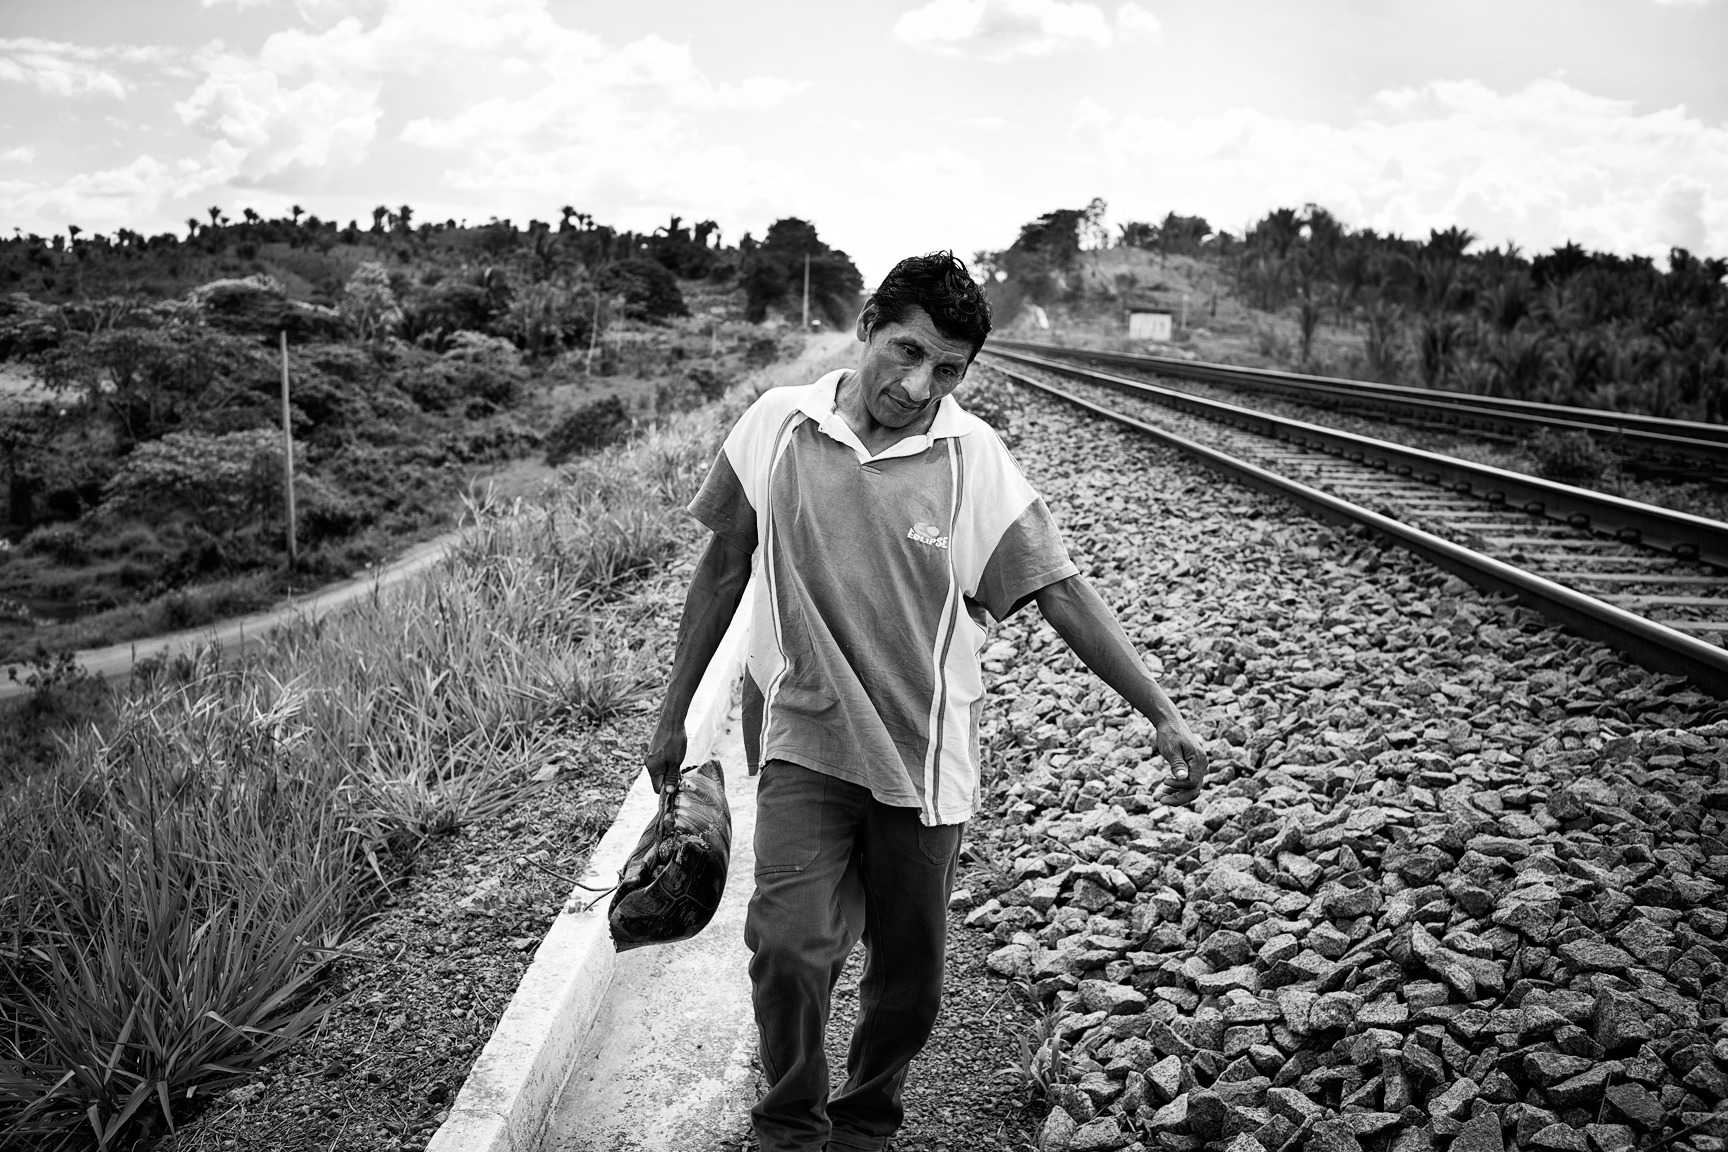
\includegraphics[width=\textwidth]{./imgs/Irakatakoa_426}
%\caption{Irakatakoa, a caminho de Altamira do Maranhão para vender um jabuti que pegou na floresta (Domenico Pugliesi, 2013).}
%\end{figure}

Os Guajá são um pequeno grupo de caçadores habilidosos, habitantes da
porção oriental da Amazônia, mais exatamente o noroeste do estado do
Maranhão. Constituíam, em 2013, uma população de 480 pessoas. 
Andarilhos, desconheciam a navegação, ocupavam
predominantemente áreas isoladas próximas a babaçuais no interior da
floresta onde, de maneira dispersa, conseguiram se manter \textit{isolados}
até o fim da década de 1980, e existem pessoas em isolamento voluntário
até os dias atuais. Sempre ocuparam os topos e ramificações das serras
do Tiracambu e da Desordem, que formam parte da região oeste maranhense,
drenadas pelos rios Turiaçu,\footnote{Bacia do Turiaçu.} Caru e Pindaré,\footnote{Bacia do
Mearim.} e rios menores como o Turi, Turizinho, rio do Sangue, rio do
Peixe, além de inúmeros igarapés formadores e tributários, como Juriti,
Mão de Onça, Maronata, Presídio, Bandeira, Mutum, Aprígio, igarapé do
Furo, do Milho, Guariba, Aparitiua, dentre outros ainda menores. Por ali
os Guajá procuraram refúgio a fim de escapar da sede durante fugas,
quando resistiam ao contato.\footnote{Para detalhes sobre a hidrografia e
topografia, ver O'Dweyer, 2010, p.\,86.}

Habitantes do que restou de floresta no estado do Maranhão, eles se
encontram na macrorregião da Amazônia Oriental e são falantes de uma
variante do tupi-guarani em um subgrupo desta família linguística
composto por nove línguas: emerillon, wayãpi, zo'e, guajá, anambé,
ka'apor, takunyapé, turiwára e amanayé (Rodrigues, 1984/\,85). Em sua
história, não tiveram aldeias permanentes e até o contato organizavam-se
em pequenos coletivos, formados por uma ou duas famílias nucleares,
dispersos sobre um território também ocupado por outros povos indígenas: Tenetehara e Ka'apor. Não dominavam cultivo agrícola algum, nem mesmo
milho ou mandioca, até o contato, e tal situação se modificou sobretudo
na década de 1990, quando a população mais jovem era \textit{ensinada}
por funcionários da Funai a cultivar mandioca, basicamente para a
produção de farinha puba, além de milho, macaxeira, abóbora e arroz.
Portanto, as roças para os Guajá pertencem aos \textit{karai}, aos
não indígenas.

Antes de tudo, os Guajá são exímios caçadores. A caça é sua principal
atividade, um tema que interessa a todos, e é nessa atividade que as
pessoas depositam grande parte de seu tempo. Caçam diversas espécies de
aves e mamíferos; detêm uma técnica extremamente apurada para a caça de
mamíferos arborícolas, em especial cinco tipos de macacos.\footnote{Macaco-prego,
cuxiú, capelão ou guariba, cairara e mão-de-ouro ou macaco-de-cheiro.} A caça em geral, e a de macacos, especificamente, é uma atividade que mobiliza toda uma aldeia: homens, mulheres e crianças.
Com a atividade da caça e o nomadismo, de tempos em tempos 
aparecem nos meios de comunicação nacionais e internacionais como os
\textit{últimos nômades caçadores-coletores do Brasil}. %e coisas do gênero.

O objetivo deste capítulo é apresentar essa história recente, baseada em
contatos e fugas, mortes na floresta e recomeços nas novas aldeias.
Histórias que os Guajá não nos deixam esquecer e são constantemente
rememoradas quando as pessoas falam de si, da família ou dos amigos.

Os Guajá provavelmente fazem parte de um histórico conjunto populacional
Tupi oriental, assemelhando-se em diversos aspectos não apenas a seus
vizinhos mais próximos, os Ka'apor e Tenetehara, mas a outras
sociedades do leste amazônico como os Asurini, Araweté, Parakanã e
Aikewara, por exemplo. ``Um complexo populacional que se estendia desde
as matas do médio Xingu até as bacias dos rios Capim, Acará, Gurupi e
Pindaré'' (Viveiros de Castro, 1986, pp.\,137--139). São povos que
historicamente ocuparam a \textit{terra firme} e que, ao sofrerem pressões
de outros povos,\footnote{As chamadas \textit{sociedades de várzea} cujo
domínio da cerâmica e técnicas de domesticação de planta era notório. Ver 
Heckenberger \textit{et al.}, 1998; Neves, 1999.} foram forçados à dispersão.
Populações como os Wayãpi, Assurini, Parakanã, Tenetehara, Zo'e,
Ka'apor, Amanajós, Anambé, dentre outros, fugiram ou desapareceram.\footnote{Viveiros de Castro, 1986, p.\,139; Gallois, 2013; Forline, 1997, p.\,29.}

``Humanos'', como encontrado entre tantos povos ameríndios, é a tradução
para \textit{awa} e funciona como um marcador enunciativo de uma condição
de pessoa (Viveiros de Castro, 2002, p.\,371). Nos dias atuais, a depender da
aldeia, se autorreferem como \textit{Awá}, \textit{Guajá}\footnote{Nome que apareceu no
contato com o Estado brasileiro.} e \textit{Awá Guajá}, mais utilizado nos
últimos anos; é difícil precisar uma designação \textit{oficial}. O fato é que
no momento atual, em que ocorrem mutirões para tirar carteiras de
identidade, as pessoas escolheram o nome \textit{Awá Guajá} para constar em
seus documentos. 

Em outras situações, no entanto, como em reuniões com
não indígenas ou \textit{karai}, ou então com os Guajajara ou \textit{kamara},
podem fazer uso de \textit{Guajá} como nome do povo. Noto aqui que a
autodenominação \textit{awa} é também utilizada por outros povos de
variante Tupi-Guarani, como os Ka'apor e Asurini. Embora Balée afirme
que sua autodenominação é \textit{Ka'apor}, o termo \textit{awa} também
funcionaria nesse contexto como sinônimo de pessoa, sobretudo com a
conotação \textit{alguém}. O termo \textit{awa}, lembra o autor, ``está
relacionado com os termos inflexivos referentes a \textit{pessoa} e \textit{povo} em
várias outras línguas tupi-guarani'' (Balée, 1998). Os Asurini do Xingu
também se autodenominam \textit{awaete}, ``gente de verdade''.

\textit{Awá}, nesse caso, teria o mesmo significado que entre os Guajá:
``humanos'', e o sufixo \textit{ete} seria um enfatizador traduzível, no
caso, Asurini e outros Tupi-Guarani por ``verdadeiro'' ou ``muito'' (Müller,
1993). Na língua guajá, o sufixo enfatizador também seria \textit{te},\footnote{Tal o \textit{ete} asurini.} tributários do conhecido sufixo
intensificador ou autentificador tupi \textit{ete}. \textit{Awatea} refere-se,
grosso modo, à humanidade próxima, ``gente de verdade'', em oposição,
por exemplo, a \textit{awa mihua}, ou ``gente braba'', designativo atribuído
aos pequenos grupos que vivem em isolamento na mata, os chamados \textit{isolados}. 

Em linhas gerais, pessoas que partilham língua e hábitos
semelhantes, porém distantes no parentesco, no espaço e na história, não
são reconhecidas como \textit{awatea}, ou ``gente de verdade''. Apesar de hoje
em dia serem utilizadas as formas \textit{Guajá}, \textit{Awá Guajá} e \textit{Awá}, uma vez que variam nas próprias aldeias, a depender da Terra Indígena e do
contexto enunciativo, por uma economia textual opto
por utilizar a maior parte do tempo o termo \textit{Guajá}, acompanhando
outros autores.\footnote{Balée, 1994, 2013; Cormier, 2003, Forline, 1997.}

\section{caçadores}

\textit{Watama'a aria}, ``nós somos caçadores'': afirmações desse tipo são
comuns entre as pessoas de diferentes aldeias. Tal condição é
expressa pelo vocábulo \textit{watama'a},\footnote{\textit{Aria}, ``nós'' que
  exclui o interlocutor (exclusivo), muito comum em diversas línguas
  indígenas.} cuja tradução literal é ``aquele que caminha''. Como
veremos aqui, \textit{andar} e \textit{caçar} são formas que podem ser expressas pelo
mesmo verbo, \textit{wata}. Os Guajá caçam na mata, dormem na mata e
passam longas temporadas na floresta, mesmo na época das chuvas. As
aldeias, tal como experimentam hoje, são resultado de uma reengenharia
social empreendida pelo contato, cujo resultado foi a reunião de
diversos grupos locais anteriormente dispersos. Muitas das famílias que
hoje vivem juntas não se conheciam pessoalmente antes do contato
oficial. As cinco aldeias existentes foram criadas a partir desta
máquina estatal de contato que marcou a ocupação da Amazônia indígena
brasileira durante a ditadura militar, sobretudo no seu fim no decorrer
da década de 1980, quando a maior parte dos Guajá foram contatados.

Trata-se de um desses grupos Tupi-Guarani do leste amazônico,
caracterizados por uma baixa complexidade material e ritual em que
elementos como a fala e o canto, cosmologia e escatologia, dentre
outros, tomam o lugar de uma economia de símbolos e práticas rituais
(Viveiros de Castro, 1986, p.\,23). Uma gente para a qual é mais fácil
produzir uma \textit{lista de ausências} de elementos \textit{típicos} (Viveiros
de Castro, 1986, p.\,47) dos povos indígenas ameríndios do que evocar uma
parafernália material que os distinga de outros povos. No que concerne à
cultura material, os Guajá não produzem cerâmica ou cestaria; seu
artesanato tradicional se resume a pequenos cocares e braceletes com
penas de tucano utilizados em um momento ritual específico; a redes e
tipoias de fibras de tucumã;\footnote{Ou \textit{tucum}.} suas casas, até o contato, eram
tapiris na floresta; não praticavam agricultura; arcos e flechas são os
únicos artefatos produzidos em profusão cotidianamente. Com exceção das
belas redes de tucum, que abrigavam por vezes uma família inteira em uma
única peça --- o casal e seus filhos pequenos ---, e uma estrutura com moquém,
uma aldeia Guajá não possuía pátio central, espaços diferenciados de
acordo com sexo ou classe de idades, caminhos e saídas para as roças ou
jardins, e era constituída por pouquíssimas pessoas, às vezes reunidas
em uma única casa.

Quanto aos marcadores sociais, os Guajá não se diferenciam muito dos
outros Tupi-Guarani orientais como, por exemplo, os Araweté. Elementos
como a divisão do trabalho fluida, simplicidade dos sistemas de
prestação e contraprestação cerimoniais ou profanos, morfologia
espacial aparentemente caótica, repertório mínimo de papéis
sociais e ausência de qualquer segmentação global\footnote{\textit{Idem}.} parecem
compor o quadro das relações cotidianas Guajá. A diferença destes para
outros Tupi do leste amazônico está, sem dúvida, em uma secular ausência
de agricultura em sua história, além do papel preponderante das mulheres
nas atividades de caça, como veremos aqui.

Sabemos sobre outras populações da mesma região que, movidas por
diferentes fatores, abandonaram as aldeias e se estabeleceram na mata,
com a vida baseada em caça e coleta e um ou outro cultivo agrícola. Nos
trabalhos de Viveiros de Castro sobre os Araweté (1986) e de Fausto
sobre os Parakanã (2001), encontra-se que nem o abandono da aldeia
permitiu que essas pessoas deixassem totalmente a agricultura.\footnote{Da mesma
forma os Huaorani do Equador. Ver Rival, 2002.} Os Araweté mantiveram o
milho, enquanto os Parakanã Ocidentais, mesmo em um \textit{trekking}
permanente, resistiram com o cultivo da mandioca em seu sistema de vida.
Os Guajá, diversamente, pelo menos durante todo o século \textsc{xx}, não se
familiarizaram com nenhum item de roça, e não há menção de conhecimento
sobre agricultura em sua história; nem mesmo os velhos se lembram de um
dia seus \textit{avós} terem plantado o que quer que fosse. 

Em contraponto a
este passado, as pessoas hoje em dia estão sendo instruídas pelos
funcionários dos antigos postos indígenas\footnote{Doravante, \textsc{pin}.} para plantar
principalmente roças de mandioca para produção de farinha, alimento pelo
qual têm grande apreço e não conheciam até o contato. Muitos contam que
os mais velhos, ao se aproximarem da Funai, se recusavam a comer \textit{taramỹ} ou farinha, pois pensavam tratar-se de \textit{wy}, ou terra. Apesar de
todas as aldeias praticarem agricultura hoje em dia com a
ajuda de mão-de-obra contratada pela Funai, a \textit{lógica} de ação ainda é
baseada na caça, e pelo menos nas aldeias em que vivi as pessoas ainda
estão dispostas a trocar uma colheita coordenada pela Funai pela mera
suspeita da existência de uma vara de porcos, ou um bando de capelães,
muitas vezes acarretando perdas significativas na produção agrícola. Por
essas características, dentre outras que ainda veremos no decorrer do
livro, os Guajá são considerados por correntes ecológicas na
antropologia parte de um grupo de pessoas, cada vez mais raro no mundo
contemporâneo, definidas, um tanto genericamente, como
\textit{caçadores-coletores} (Lee and Daly, 1999).

Tais observações remetem a uma discussão clássica da etnologia
americanista referente à existência e pertinência da ideia de povos
caçadores-coletores na América do Sul tropical. Na história da etnologia
sul-americana, por exemplo, dentre tantos outros coletivos como os
Nambikwara e os povos de língua maku, duas sociedades, ambas
Tupi-Guarani, foram constantemente citadas como paradigmáticas quando o
tema era caça e coleta: Aché e Sirionó. Por terem sido algo como um
\textit{modelo} nessa discussão, os Aché despertaram o interesse de
sociobiologistas pela busca de revelar como o grupo conservara
\textit{características do Paleolítico} em pleno século \textsc{xx} (Hill \& Hawkes,
1983). Tais pesquisadores classificaram os Aché algo como sobreviventes
da pré-história, a despeito da revolução neolítica, e de a agricultura
ser amplamente praticada na Amazônia (Roosevelt, 1992, p.\,202). Em diversas
análises\footnote{Lévi-Strauss, 1970, pp.\,121--139; Service, 1971; Viveiros de
Castro, 1986, p.\,106; Balée, 1999; Fausto, 2001), os Sirionó (assim como os
Aché.} estão presentes como fiéis representantes desses pequenos bandos
de caçadores nômades, dotados de uma estrutura social quase amorfa.
Sirionó, Aché e também Guajá desenvolveriam aquilo que Clastres
criticamente denominou \textit{economia da miséria} (2004 {[}1976{]}, p.\,178).

A Amazônia e outras terras baixas sul-americanas eram vistas como
universos puramente naturais, onde os povos mais aptos a ocupar esse
ecossistema seriam os chamados caçadores-coletores (Balée, 1992). De
alguma forma, uma vez que durante milhares de anos da história humana em
algum momento a humanidade viveu de caça e coleta, gradativamente
substituídas pela agricultura há cerca de dez a cinco mil anos,\footnote{Neves,
1988 \textit{apud} Balée, 1992.} cientistas com diferentes orientações, como se
estivessem à procura de nossas origens, ``consideram que a pesquisa
sobre caçadores-coletores modernos, tais como os da Amazônia, poderia
elucidar padrões de utilização de recursos por parte de nossos
antepassados pré-agrícolas'' (Balée, 1992). Tal ideia é utilizada pela
ciência a fim de ilustrar quase que uma espécie de \textit{elo perdido} e
sustenta que a humanidade, em algum período de sua história, foi por
completo formada por povos caçadores-coletores (Ingold, 2003, p.\,123).

\section{povo do cocal}

Os Guajá estão inseridos em uma área onde espécies botânicas utilizadas
como recursos primários só se tornaram dominantes e/\,ou frequentes em
regiões onde havia intervenção humana direta, sobretudo na agricultura, 
e boa parte dos espaços supostamente \textit{naturais} pode
ter tido um passado agrícola, conectando povos sem agricultura a uma
cultura de capoeira (Balée, 1992). E, também, as matas amazônicas estão
longe de serem \textit{primordiais}, diferentemente das ``teorias
adaptacionistas em ecologia cultural, que assinalam que grupos indígenas
da Amazônia se adaptam às condições e respondem aos limites
meio-ambientais'' --- a floresta e outros \textit{habitats} amazônicos não
são somente de origem \textit{natural}. Em suas estimativas, o autor
considerava que \textit{pelo menos 11,8\% da mata de terra firme na Amazônia
brasileira é antropogênica} (Balée, 1987). Como um exemplo, Balée
seleciona justamente o caso Guajá:

\begin{quote}
Os Guajá são um dos últimos grupos forrageiros da América do Sul{[}\ldots{}{]} 
Tradicionalmente, procuravam comida em grupos de cinco a dez
pessoas em uma mata dominada, na sua maior parte, por árvores das
famílias da Castanheira-do-Pará, beru, faveira e abiu. Nunca derrubaram
ou queimaram a mata, fazendo seus acampamentos temporários
exclusivamente em cocais{[}\ldots{}{]} Os cocais onde os Guajá acampam e
percorrem contêm, praticamente sempre, vestígios de aldeias e roças
antigas de outros grupos indígenas da região, como os Urubu-Kaapor, que
habitam na fronteira leste de suas terras.\footnote{Balée, 1987, p.\,2.}
\end{quote}

Por terem sofrido um processo de \textit{perda} do domínio agrícola devido a
efeitos de guerras, epidemias e colonização, adotaram um estilo de vida
baseado na caça e coleta (Balée, 1994; 1999). O termo \textit{regressão
agrícola}, trabalhado por Balée, é utilizado a fim de ilustrar a
transição de uma organização econômica ligada à horticultura para a caça
e coleta, dois \textit{modos de produção} complementares e compreendidos na
história como dois momentos diversos: um, marcado por menos
pressões externas, o que favoreceria a sedentarização; e outro, em razão
das tais pressões, marcado pela mobilidade territorial, trazendo
mudanças à antiga vida sedentária que, deixada para trás, poderia ser
retomada de acordo com acontecimentos futuros. Embora alguns desses
caçadores-coletores na América do Sul permaneçam com um conjunto de
plantas semidomesticadas, há a hipótese de que os vegetais cultivados
nessa transição \textit{desaparecem} gradualmente; somente alguns gêneros são
mantidos, embora seu cultivo caia consideravelmente --- como é o caso do
milho entre os Sirionó (Balée, 1994, p.\,210).

É inescapável em análises como esta a atmosfera de arcaísmo, sugerida de
maneira indireta pela ideia de regressão. Rival, por exemplo, a critica,
ao afirmar que a tal \textit{passagem} de um estado a outro é algo como uma
\textit{estratégia}, porém muito mais ampla e dinâmica do que uma resposta
à Conquista portuguesa ou espanhola na América do Sul (Rival, 2002, p.\,13).
Embora noções como \textit{forrageio ótimo} (Ingold, 2002,
pp.\,27--39) não terem sido operativas para esse autor como foi para outros
(Hawkes, Hill \& O'Conell, 1982), a ideia de \textit{regressão agrícola}
supervalorizaria o \textit{sedentarismo} em detrimento do tipo de vida que
povos como os Guajá levavam, baseadas em muitos deslocamentos pelo
território. É como se, uma vez que as pessoas pudessem optar,
decidiriam não mais andar, numa correlação direta entre ausência total
de agricultura e mobilidade territorial. De acordo com a crítica de
Rival:

\begin{quote}
Balée, portanto, correlaciona a ausência de agricultura com a
mobilidade {[}territorial{]}. Povos que cultivam intensivamente não possuem
grande mobilidade territorial; de modo inverso, povos que caçam e
coletam são altamente móveis. Embora eu concorde com sua insistência da
mobilidade ser considerada uma estratégia adaptativa histórica, ao invés
de somente uma imposição ambiental, lamento que o autor negligencie
dinâmicas históricas pré-conquista desencadeadas por conflitos entre
populações nativas altamente móveis e outras menos móveis.\footnote{Rival, 2002, p.\,13, livre tradução.}
\end{quote}

As plantas selvagens das quais dependem os Guajá são, por assim dizer,
semidomesticadas, uma vez que estão em áreas de capoeira, ou capoeiras
velhas, áreas antropizadas. Balée procura paralelos entre o conjunto
Tupi-Guarani contemporâneo e sustenta três pontos: (1) os grupos \textsc{tg} forrageiros contemporâneos passaram por um processo de regressão agrícola perdendo o domínio de todas as plantas domesticáveis, inclusive
do milho; (2) entre as plantas utilizadas, as diversas espécies de palma
ocupam papel central, tanto na alimentação quanto como matéria-prima; e (3)
algumas dessas palmas,\footnote{Jerivá e Mucajá {[}no Paraguai{]}, na região
sudoeste do Brasil {[}no Paraná{]}, onde habitavam os Hetá, assim como Babaçu,
Inajá e Tucumã.} presentes no território Guajá, são, devido a
predominância e frequência, indícios de presença pretérita de
horticultura\footnote{Balée, 1994, p.\,218.}.

De acordo com esse autor, grupos
amazônicos que baseiam suas atividades no forrageio são capazes de viver
na floresta tropical sem o cultivo de roças graças a alguns recursos
essenciais, como palmas e frutos, principalmente. Estes são subprodutos de
ocupação humana remota, e um padrão baseado na caça e coleta está
diretamente ligado à distribuição desses recursos no ambiente. A crítica
que fazemos é a mesma de Rival, pois nessas florestas bioculturais a
intencionalidade desses atos é sempre atribuída a uma \textit{inteligência}
passada, resultado de um conjunto de manejos anteriores (Rival, 2002, p.
13).

Não cabe a este livro advogar contra modelos da ecologia política e da
ecologia histórica, e, independentemente das teses
regressivas ou involutivas ou da pertinência em pensar uma mudança do
\textit{modo de produção forrageiro} para a agricultura, o objetivo
aqui é apresentar etnograficamente os processos de transformação pelo
qual vêm passando os Guajá. Esta suposta passagem entre modos de
produção tem sido experimentada pelas aldeias de uma maneira bastante
particular, como veremos mais abaixo; e, mais do que pensar uma mudança
no modo de produção, o que aparece aqui
são formas de se alimentar e agir como um novo tipo de gente. Uma gente
que sabe falar a língua dos \textit{karai} ou ``não indígenas'', bastante
interessada em uma nova humanidade encontrada a partir do contato e que
faz uma leitura criativa do que seja o, assim chamado, \textit{trabalho na
roça}.

Desde o contato, a Funai operou uma transformação radical na vida das
pessoas. Além de uma sedentarização dos pequenos coletivos, podemos
falar em uma espécie de \textit{kit pacificação}, a partir do qual a farinha
de mandioca, as espingardas e os cachorros foram, muito rapidamente,
incorporados à vida nas aldeias e de muitas maneiras, como veremos nesse
livro, ganharam um papel de destaque.\footnote{As armas de fogo, por
  exemplo, que foram introduzidas nas comunidades entre os anos de
  1970--1980 por funcionários da Funai e toda sorte de agentes que
  participaram dos primeiros contatos, tornam-se hoje uma ferramenta
  fundamental na caça, ao passo que, devido à lei federal do Estatuto do
  Desarmamento (Lei 10826, de 22 de dezembro de 2003), a mesma Funai que
  introduziu armas e munições nas aldeias é impedida de fornecer tais
  itens às comunidades, não importando quão isoladas elas sejam.} Junto
a esse processo de mudança, a ideia de que podem plantar sua própria
comida, frente a um passado de caça e coleta, aparece como um elemento
central e controverso, como veremos mais abaixo.

\section{ecologia e ferrovia}

A população Guajá é estimada em 420 pessoas\footnote{Segundo o último censo que
realizei em 2013.} que vivem em cinco aldeias --- Juriti, Tiracambu, Awá, Aldeia Nova e Cocal/\,Guajá --- distribuídas por três áreas indígenas. Algumas aldeias adotam nomes análogos aos postos da Funai,
por isso não seriam nomes elaborados pelas comunidades, mas adequados
pelos postos. Apesar de ter conhecido todas elas, meu trabalho de campo
foi realizado nas aldeias Tiracambu, Awá e Juriti, e durante os
anos de doutorado passei a maior parte do tempo de pesquisa na aldeia
Juriti.

% %\textbf{Mapas}
% \begin{figure}[t]
% \centering
%   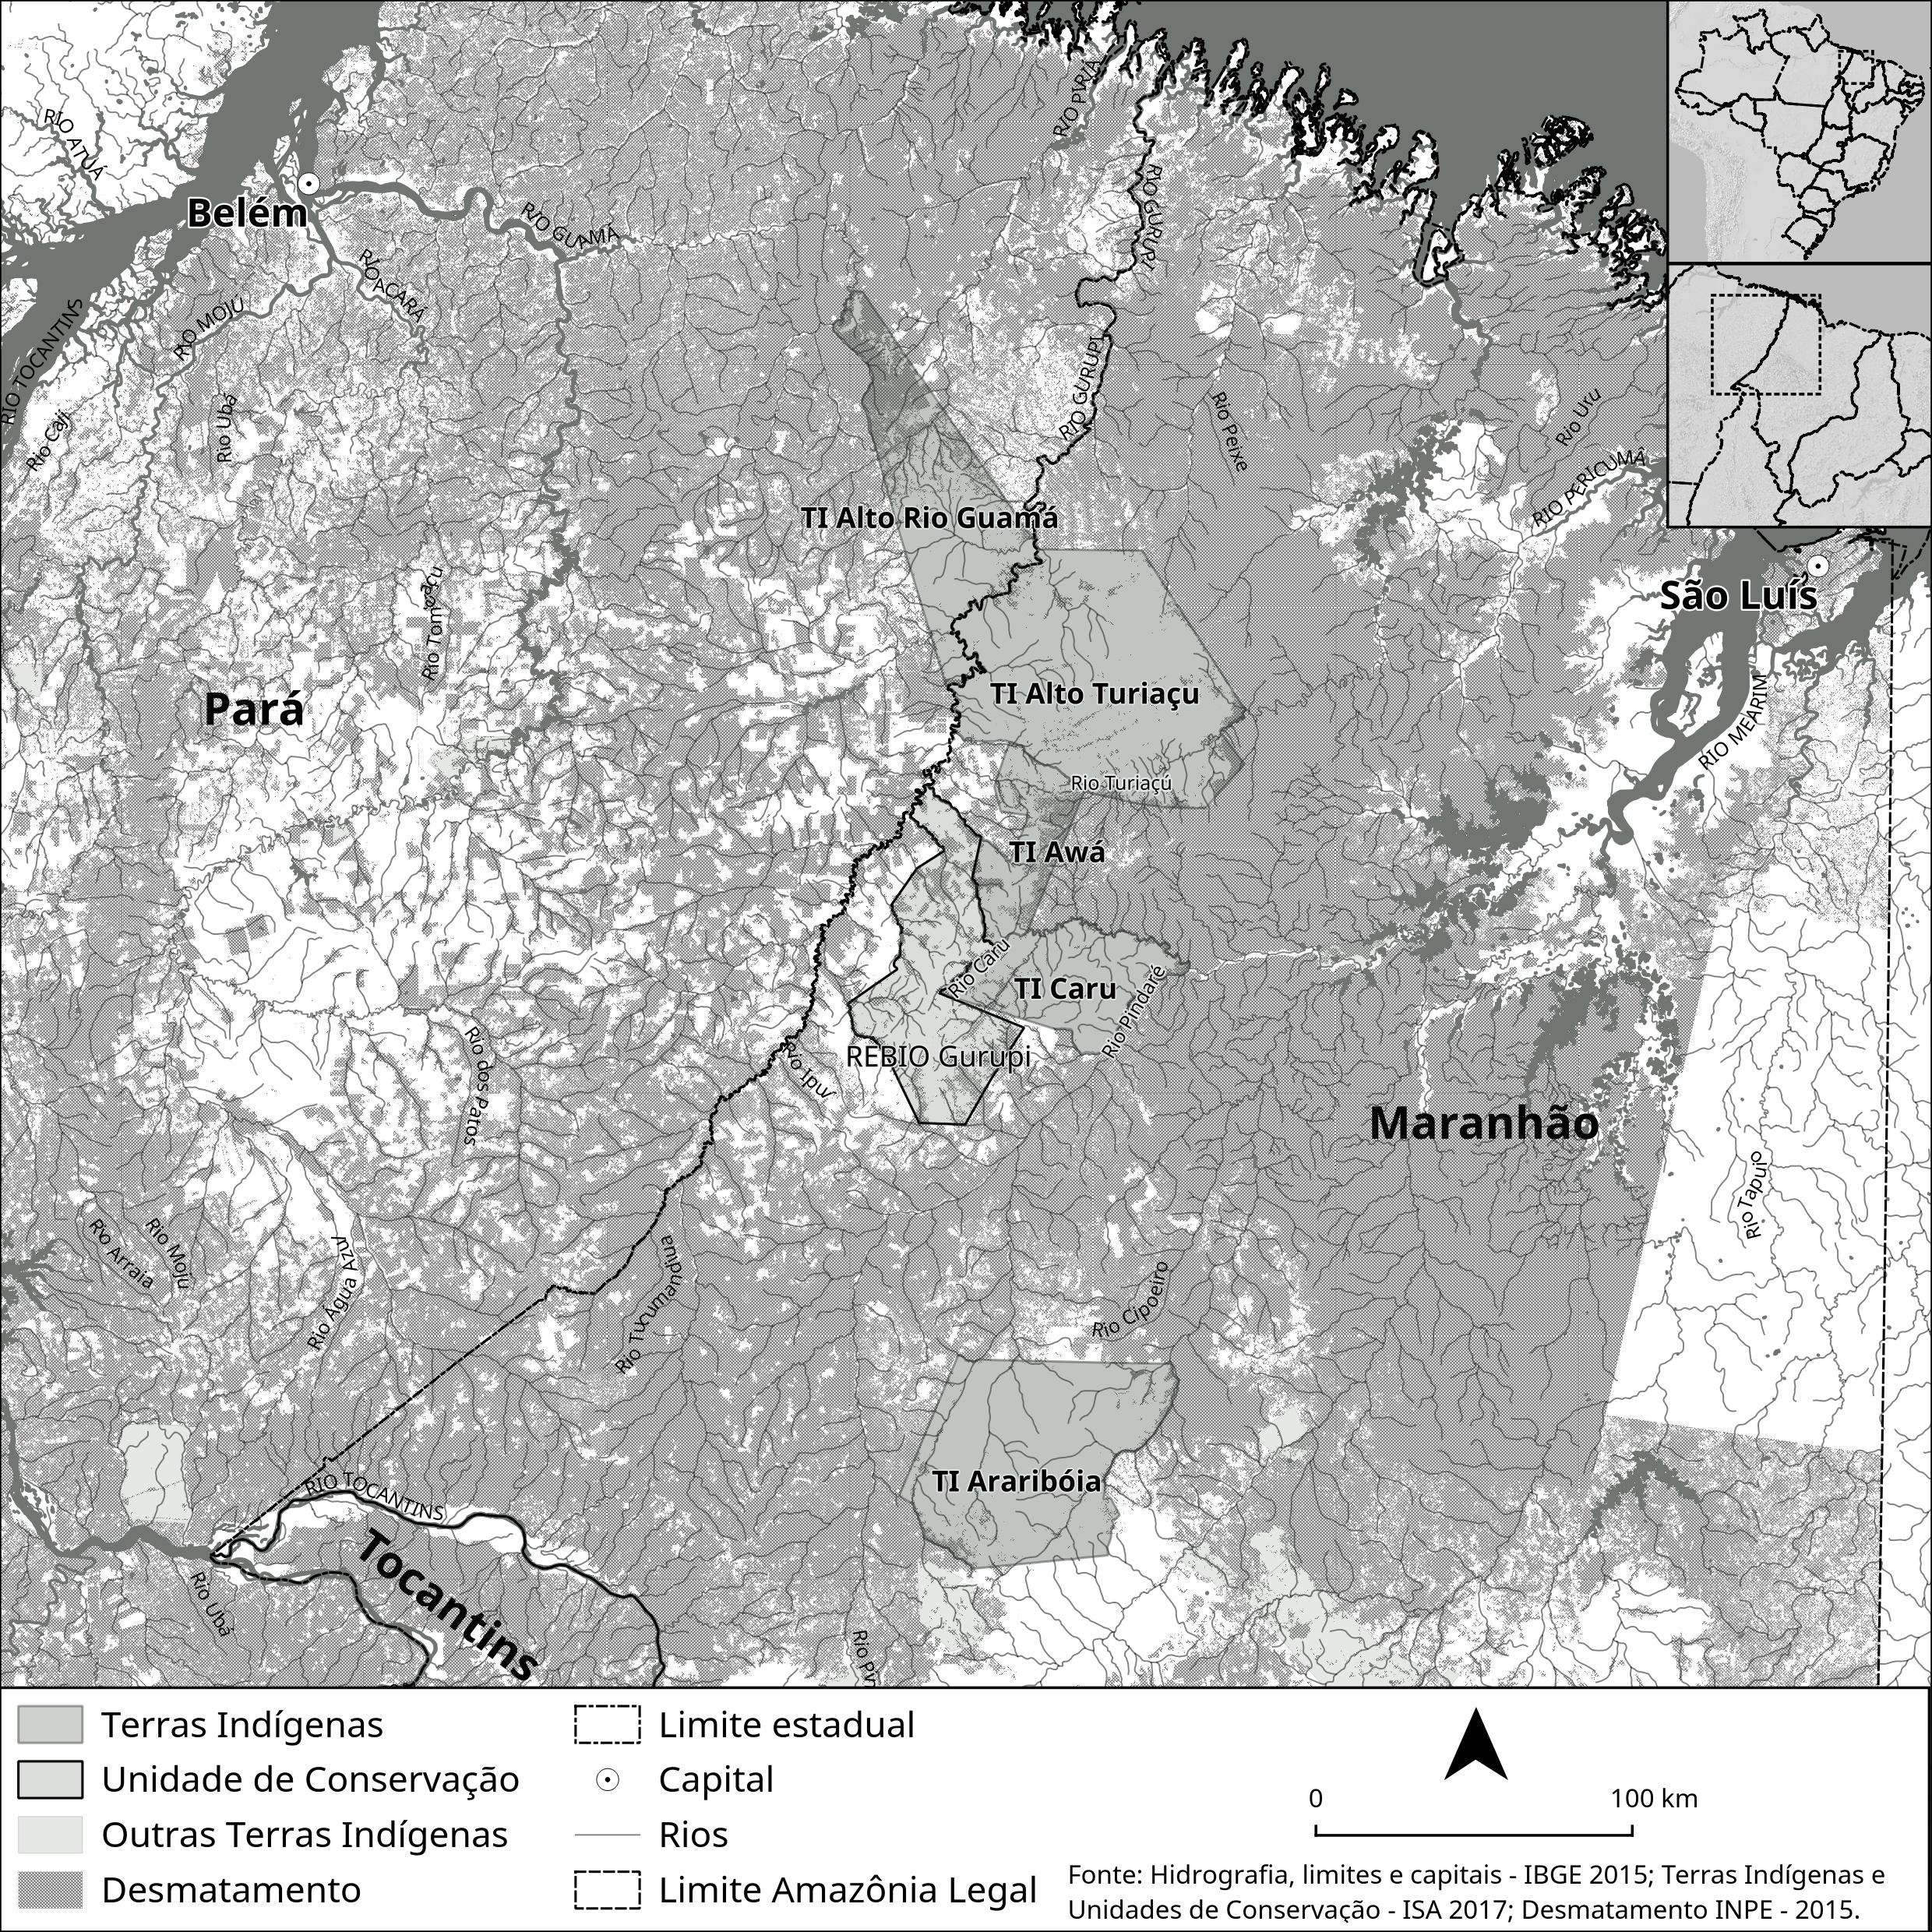
\includegraphics[width=\textwidth]{./imgs/mapa_livro_uira}
% \caption{Mapa. Créditos: Tiago Moreira dos Santos/\,Instituto Socioambiental (\textsc{isa}).}
% \end{figure}

%À exceção da área indígena Awá (\textsc{ti} Awá), onde se situa a aldeia Juriti,
%os Guajá dividem suas \textsc{ti}s com outros quatro grupos indígenas: Tenetehara
%(Guajajara e Tembé), Ka'apor e alguns Timbira. No caso da área Carú, os
%Guajajara estão em maioria, e possuem cinco aldeias, enquanto os Guajá,
%na mesma área, formam três aldeias: \textit{Awá}, Tiracambú e Aldeia Nova.
%Caso semelhante ocorre na aldeia Guajá, na terra indígena Alto Turiaçú,
%área em que os Ka'apor estão em maioria. Nesta \textsc{ti}, além dos Guajá e
%Ka'apor, os Tembé (Tenetehara) também se fazem presentes, havendo ainda
%um pequeno grupo Timbira. Nos último anos ocorreram casamentos de alguns
%Guajá com Ka'apor ou Guajajara.

%Suprimido a pedidos do autor

A área indígena Awá, onde se situa a aldeia Juriti, representa a única
área demarcada exclusivamente para os Guajá; a \textsc{ti} Alto Turiaçú foi
pensada inicialmente com uma área Ka'apor, e a área Caru, para usufruto
dos Guajajara. Atualmente, pela necessidade de estabelecer uma
convivência menos belicosa,\footnote{Parte dos dois povos divide o
mesmo território há décadas.} os Guajá e Guajajara da \textsc{ti} Caru procuram
estabelecer alianças políticas, principalmente frente às reivindicações
dirigidas à Funai/\,\textsc{sesai}. No entanto, ao mesmo tempo algumas pessoas das
aldeias Guajá observam que tais alianças caracterizam uma tentativa de
controle dos Guajajara sobre as decisões dos Guajá, inclusive com
propostas de alguns Guajajara chefiarem postos indígenas de aldeias
Guajá.

Desde os últimos 150 anos estima-se que estejam nos arredores dos rios
Pindaré, Turiaçu e Gurupi, tendo este último rio sua área de
predominância na porção oeste do Maranhão. Essa região em que vivem tem
como limite o Rio Gurupi a oeste, o Oceano Atlântico ao norte, o alto
curso dos rios Pindaré, Grajaú e Gurupi ao Sul e, a leste, a margem
esquerda do Rio Mearim; nenhum desses rios é tributário do Amazonas.
Além dos Guajá, vivem na região os Ka'apor ou Urubu, Tembé e Guajajara
(Balée, 1994, p.\,10), dividindo-se em três áreas contíguas: ao sul, a
Terra Indígena (\textsc{ti}) Caru, com 172.600 hectares ocupados conjuntamente com os
Guajajara; ao norte, a \textsc{ti} Alto Turiaçu, com 530.500 hectares, em companhia dos
Ka'apor e alguns Tembé; e, entre as duas, a \textsc{ti} Awá, com 118.000 hectares
(Cormier, 2000, p.\,11). Além dessas três, alguns indivíduos habitam a
Terra Indígena Arariboia (Guajajara) e a \textsc{ti} Alto Rio Guamá (dos Tembé),
contígua à \textsc{ti} Alto Turiaçu (Cormier, 2000, p.\,11).

A porção de floresta amazônica no \textsc{ma} é um cenário com alto grau de
pressão antrópica, e a vida desses coletivos se desenrola na única
região de floresta tropical que ainda resta no estado, formando um
conjunto de terras indígenas e uma Unidade de Conservação que estão na
lista das mais desmatadas da Amazônia Continental. De acordo com estudos
recentes (Martins \& Oliveira, 2011), as áreas indígenas são as únicas
áreas de floresta que restaram a ser preservadas, ao lado da Reserva
Biológica do Gurupi, no estado do Maranhão. 

Trata-se, na Amazônia, de
uma região com uma das porções mais expressivas em termos de riqueza de
espécies e endemismos, onde se localiza mais da metade do Centro de
Endemismo Belém (Martins \& Oliveira, 2011, p.\,20) e se abrigam animais
ameaçados de extinção, como a ararajuba,\footnote{\textit{Guarouba guarouba}.} o gavião real,\footnote{\textit{Harpia harpyja}.} o araçari,\footnote{\textit{Pteroglossus
bitorquatus bitorquatus}.} e a jacupiranga,\footnote{\textit{Penelope pileata}.} além de duas espécies de primatas da Amazônia oriental, o \textit{Cebus kaapori}, ``Cairara
Ka'apor'', e o \textit{Chiropotes
satanás}, ``Cuxiú́-preto'', todos ameaçados de extinção. De acordo com o \textsc{icmb}io, das 46
espécies listadas por pesquisadores como ameaçadas de extinção na
Amazônia, mais de 50\% estão presentes no Centro de Endemismo Belém.

Além dos Guajá, Tenetehara e Ka'apor, todos povos de língua tupi, no oeste do
Maranhão, mais ao sul, há ainda os Ramkokamekra-Canela e
Apaniekra-Canela, os Krikatí e Pukobyê, falantes de línguas do tronco
macro-jê; de modo geral, em toda a região oeste do estado do Maranhão há
porções ocupadas por povos indígenas. Tal região é composta por cidades
antigas como Pindaré-Mirim, pelo surgimento de novas aglomerações ao
longo das Rodovias \textsc{br}--316, Belém--Teresina, e \textsc{br}--010, Belém--Brasília, e
pelo rápido crescimento de outras, como é o caso de Santa Inês. Trata-se
de uma região onde migrantes do nordeste do país e do próprio Maranhão
promoveram uma ocupação à base de unidades de produção familiar,
sobretudo a partir da agricultura de corte e queima, que até hoje é
praticada com intensidade. Trata-se de uma grande área, compreendida
pelas microrregiões do Gurupi, Pindaré, Imperatriz, Alto Mearim e
Grajaú, marcada por um rápido crescimento populacional e uma
avassaladora ocupação territorial (Diniz, 2005).

Todo o território Guajá incide na macrorregião onde foi implantado o
Projeto Carajás (\textsc{pgc}),\footnote{O Projeto Carajás, oficialmente conhecido
  como Programa Grande Carajás (\textsc{pgc}), é um projeto de exploração mineral
  iniciado em 1980 na mais rica área mineral do planeta, pela Vale
  (antiga \textsc{cvrd}). Estende-se por 900 mil quilômetros quadrados, uma área que corresponde a
  um décimo do território brasileiro, é cortada pelos rios Xingu,
  Tocantins e Araguaia e engloba terras do sudeste do Pará, norte de
  Tocantins e sudoeste do Maranhão. Foi criado pela empresa estatal
  brasileira Companhia Vale do Rio Doce --- durante o governo Figueiredo ---
  quando Eliezer Batista era seu presidente.} cuja
ferrovia para transportar sobretudo minério de ferro foi inaugurada em
1985, fazendo com que o contato com grupos que viviam isolados ou
\textit{arredios}, segundo a terminologia da época, fosse acelerado. Na
ocasião, os contatos com os grupos Guajá ainda estavam sendo iniciados,
e centenas de indivíduos sem contato morreram vitimados por doenças e
assassinatos provenientes do \textit{boom} populacional que houve na
região, propiciado pela construção da ferrovia. A Estrada de Ferro
Carajás (\textsc{efc}) cortou o território tradicional Guajá, provocando não
apenas a perda de suas terras, mas a dispersão e a morte dos animais de
caça e o fim de boa parte das florestas do oeste maranhense. Foi esse
mesmo fenômeno, aliado à concomitante ocupação da região, dado o
crescimento de vilas e povoados, que produziu a divisão de muitos grupos
locais, pelo que alguns remanescentes experimentam até os dias de hoje
uma vida sem contato com outros grupos.

O Projeto Carajás, que não afetou apenas os Guajá, mas cerca de 40
comunidades indígenas diferentes (Treece, 1987), tem importância direta
na configuração socioespacial dos povos indígenas da região atualmente.
O impacto da estrada de ferro, inaugurada em 1985, é sentido pelos Guajá
não apenas pela presença física da ferrovia e o \textit{boom} populacional
decorrente que continua se intensificando devido ao projeto atual de
duplicação da ferrovia, mas também pelos transtornos ecológicos que
modificaram as atividades de caça (Garcia, 2014\,\textsc{b}). O impacto social, com
o adensamento populacional, forçou por um lado a fuga e dispersão às
cegas de muitos grupos locais que ali viviam, e por outro, nos últimos
20 anos, a concentração de pessoas até então separadas em
grandes aldeias com até 200 habitantes, como é o caso da aldeia
Awá, na \textsc{ti} Caru --- algo que os Guajá não conheciam em sua história
até então. As poucas iniciativas de ajustes ao impacto do contato e ao
desastre ambiental, há tempos anunciado para a Amazônia Oriental, foram
mal administradas. Escândalos de desvios de verba do \textit{Programa Awá},
projeto financiado pela mineradora até então estatal Companhia Vale do
Rio Doce (\textsc{cvrd}), durante as décadas de 1980 e 1990, criado a fim de
mitigar os impactos de suas ações na região, deram a tônica da atuação
da Funai até meados dos anos 2000.

Dado o impacto que a construção da estrada de ferro Carajás traria, e
trouxe, às comunidades indígenas em sua área de influência, foi
estipulado que parte dos recursos do projeto, de 300 milhões de dólares, seria
aplicada em programas de assistência para esses povos, em forma de um
convênio entre a Funai e a antiga \textsc{cvrd}. Uma das principais exigências
com relação à construção da ferrovia era a manutenção da integridade dos
territórios indígenas afetados e o desenvolvimento de iniciativas que
garantissem a qualidade de vida de seus habitantes. Além dos Guajá e
Guajajara, a ferrovia causou impacto em diversas outras comunidades,
como os Xikrin, Gavião, Ka'apor e Suruí, pelo que a \textsc{cvrd} foi obrigada a
manter projetos de compensação.

No caso específico dos Guajá, esse convênio foi um fracasso, visto que
mais de 20 anos se passaram para que a \textsc{ti} Awá, onde se encontra a aldeia
Juriti, fosse homologada: tempo suficiente para causar inúmeros
transtornos decorrentes das invasões e exploração ilegal desse
território. Enquanto isso, os programas de saúde que vieram com as
frentes de contato não se preocuparam com os riscos evidentes diante da
fragilidade das pessoas contatadas. A intenção parecia ser contatar a
qualquer custo, de qualquer maneira, no ritmo desejado pelas
empreiteiras. Os primeiros contatos, sem os cuidados necessários,
resultaram na morte de vários indivíduos, e entre 1976 e 1980 morreram
aproximadamente dois terços dos residentes do \textsc{pin} Guajá\footnote{O primeiro a
ser criado, ainda em 1976.} por doenças introduzidas, principalmente
malária e a gripe. A contratação de terceiros também não foi realizada
sob critérios satisfatórios. Muitos funcionários novos e temporários da
Funai não foram submetidos a exames médicos, situação que muitas vezes
trouxe enfermidades e óbitos. 

Fora isso, muitos observadores comentaram
que os recursos que outrora deveriam ser destinados aos objetivos
originais do convênio foram aplicados em infraestrutura para a própria
Funai. Tempos depois foram criados outros convênios entre a Funai e a
antiga \textsc{cvrd}, desenvolvidos com interrupções e uma quantidade de recursos
menor do que o montante original. Passavam-se períodos em que a \textsc{cvrd}
apenas fazia pequenas caridades às comunidades Guajá. Um dos últimos
episódios, que veio à tona nos anos de 2001 e 2002, foi um grande desvio
de recursos da compensação por parte de um funcionário da antiga \textsc{cvrd} e
o até então chefe do núcleo de apoio da Frente de Atração em Santa Inês.
Até ser descoberta a fraude a saúde Guajá ficou bastante comprometida, e
o dinheiro que deveria ser posto à disposição dos indígenas desapareceu.
Apesar de os fatos terem sido parcialmente apurados pela Justiça, com a
demissão do funcionário da \textsc{cvrd} envolvido no esquema e a condenação do
servidor da Funai, os Guajá nunca recuperaram o montante desviado. Até
os dias de hoje, todo os recursos que entram por meio da Funai para as
aldeias Guajá são oriundos desse convênio.

Em decorrência desse megaempreendimento, a população regional cresceu
junto com o número de povoados ao longo da estrada de ferro. Tal pressão
demográfica aumentou o número de invasões nas áreas indígenas adjacentes
e intensificou o movimento dos trens da, agora, Vale, espantando a caça
e interferindo diretamente na vida de várias comunidades Awá Guajá e
Guajajara, já que a ferrovia margeia o perímetro sul da área indígena
Caru, junto ao rio Pindaré, como pôde ser observado no mapa acima.
Frente a tantos problemas, em várias ocasiões a estrada de ferro Carajás
foi fechada por um conjunto de povos insatisfeitos com o atendimento da
\textsc{sesai}, Funai, Vale ou demandas mais abrangentes ligadas aos indígenas.

O epílogo dessa história ainda não pode ser vislumbrado, mas os
desdobramentos não poderiam ser mais sinistros. Desde 2010 foi iniciada
a duplicação da \textsc{efc}, levada a cabo por grandes empreiteiras, como a
Camargo Correa, empreendimento que passa beirando toda a extensão sul
da terra indígena Caru, e um novo convênio de compensação, além de um
gigantesco Plano Básico Ambiental (\textsc{pba}) está em curso incidindo nas
aldeias Guajá e Guajajara da \textsc{ti} Caru, e na \textsc{ti} Rio Pindaré, dos
Guajajara. Os recursos são volumosos, apesar de estarem aquém do real
impacto dessa obra na vida das pessoas. Além disso, como podemos ver no
mapa da região, a \textsc{ti} Caru faz parte de um grupo maior de áreas que
deveriam ser protegidas, tal como vem sugerindo o grupo de trabalho
coordenado por Marlúcia Martins que congrega pesquisadores do Museu
Paraense Emílio Goeldi, e outras instituições governamentais e
não governamentais, através do que vem sendo chamado de Mosaico do
Gurupi, uma área de gestão territorial. Diversas características
particulares de diversidade e endemismos, como já ressaltei,
justificaria pensar as \textsc{ti}s e a Reserva Biológica (\textsc{rebio}) do Gurupi de
maneira conjunta. E mais, nesse mosaico, como se pode notar no mapa, a
\textsc{ti} Awá é estratégica por ser o \textit{corredor} que ligaria os dois blocos
de áreas protegidas, mais ao norte e mais ao sul. O \textsc{pba} da duplicação de
uma estrada de ferro voltado para uma única área indígena, quando a
estrada beira todo um Mosaico é, além de incompleto e mesquinho,
prejudicial ao funcionamento de todo um ecossistema que está entre os
mais ameaçados da zona tropical. Como investir em uma única área (Caru) 
quando as outras quatro (Awá, Alto Turiaçú, Alto Rio Guamá e \textsc{rebio} do
Gurupi) estão desguarnecidas e completamente invadidas?

\section{breve histórico}

Caçadores, habitantes das terras firmes do noroeste maranhense, os Guajá
se encontram nas franjas da floresta amazônica, em uma região de
ocupação Tupi-Guarani que vai desde as matas do Xingu, sobe pelo
Tocantins, atravessa os rios Capim, Acará e Gurupi e chega até o
Pindaré. Gomes (1982), por exemplo, defende que uma das hipóteses mais
prováveis é a dos Guajá terem chegado na região na \textit{esteira} dos
Ka'apor, grupo historicamente inimigo, que também migrava para a região
do rio Turiaçu. Até o século \textsc{xix} poderiam ser encontrados na porção
leste do estado do Pará e provavelmente atravessaram o Rio Gurupi
chegando ao atual Maranhão no final daquele século,\footnote{Ver Balée, 1994.} e
lá encontraram os Tenetehara, possíveis descendentes dos Tupi da costa
maranhense. Sabe-se também que estão desde o século \textsc{xix} pelas cabeceiras
dos rios Pindaré, Turiaçu e seus tributários (Gomes, 1982). Há outros
relatos que afirmam existirem grupos Guajá nas imediações do Pindaré e
Turiaçu há pelo menos 150 anos. Isso é discutido por Gomes (1985) e
retomado por Cormier (2003) ao defenderem que a menção mais antiga ao
nome deste povo data de 1853, notificado pelo presidente da província do
Maranhão, quando eles foram vistos às margens de afluentes do Caru e
Gurupi.

De acordo com o missionário José Noronha (1856), pelo menos 18 grupos
indígenas diferentes ocuparam as bacias Tocantins-Araguaia na região de
encontro entre o baixo Tocantins e a \textit{boca} do Araguaia (Balée, 1994,
p.\,25), na atual região em que hoje estão municípios como Imperatriz
(\textsc{ma}), Marabá (\textsc{pa}) e Paraupebas (\textsc{pa}), desde
o ano de 1767. E na região da
margem esquerda do Tocantins, Noronha menciona um grupo, segundo ele
denominado \textit{Uayá}, que, de acordo com Balée (1994), podem ser os
antecedentes dos atuais Guajá (Balée, 1994, p.\,25). O problema do
argumento do autor reside tanto no fato de o termo \textit{Guajá} não fazer
parte do léxico da língua nativa --- termo oriundo de fora --- como por
\textit{awa}\footnote{Uma outra palavra da qual \textit{Uaya} pode ter surgido.} ser
um vocábulo tupi muito utilizado não só entre os Guajá, mas entre outros
povos de língua tupi-guarani, como já mencionei.

Nimuendajú (1948) menciona alguns relatos, entre eles o de Francisco
Xavier Ribeiro Sampaio (1825), que em 1774 menciona entre os grupos
indígenas do baixo Tocantins os \textit{Uayá}. Outro autor apresentado por
Nimuendajú, Cezar Augusto Marques (1864), menciona os \textit{Ayaya}, um
povo \textit{selvagem} que se encontrava nas imediações da estrada que ligava
Imperatriz a Belém. E, de acordo com Araujo Brusque (1862, p.\,12), os
\textit{Uaiara} ou \textit{Guajará}, segundo Nimuendajú, podiam ser vistos no
alto curso do rio Gurupi, mas não fixaram residência naquela região
(Nimuendajú, 1948). Anos depois, em 1873 foram noticiados novamente pelo
engenheiro Gustavo Luís Guilherme Dodt, que viajou pela região do Gurupi
na segunda metade do século \textsc{xix} e em 1873 publicou seu relato, reeditado
em Dodt (1939).

Sabemos que a vasta região entre os rios Xingu e Tocantins, ``na altura
do médio-baixo curso de ambos, era ocupada por diversos grupos
Tupi-Guarani'' desde o século \textsc{xvii} (Nimuendajú, 1948, \textit{apud} Viveiros de
Castro, 1986), enquanto na margem direita do Tocantins estavam povos
não Tupi, como os Apinajé, Timbira e uns tais Acarajá-pitanga. Os grupos
Tupi se encontravam na margem esquerda do Tocantins (Balée, 1994;
Noronha, 1856), e presume-se que os Guajá sejam provenientes do que é
hoje o sudeste do estado do Pará, entre os rios Araguaia e o baixo curso
do Tocantins. Tal como outros povos Tupi-Guarani, os Guajá também
parecem ser provenientes do interflúvio Tocantins-Xingu, cujos alguns
povos migraram pelo leste amazônico,\footnote{Por exemplo os Araweté, Parakanã e Asurini.}
outros se deslocaram para o extremo leste\footnote{Ka'apor e Guajá.} ou ainda se
encaminharam para o norte\footnote{Waiãpi.} e meio-norte\footnote{Zo'e.} amazônico, tudo
ao longo dos últimos três séculos (Viveiros de Castro, 1986; Gallois,
1988; Balée, 1994). 

As causas para esta migração são desde guerras com
povos vizinhos até o encontro das populações nativas com a máquina
colonial que ocupou boa parte dos territórios indígenas. Balée cita,
para o caso Ka'apor, que uma epidemia de varíola e a guerra da
Cabanagem, ocorrida entre 1835 e 1836, acelerou a ida dos Ka'apor para a
bacia do Gurupi, no nordeste do Pará. Alguns povos provavelmente
originários deste conjunto Tupi-Guarani podem ser hoje encontrados tanto
no Pará quanto no Maranhão, e a dispersão dos povos desta família
linguística, iniciada a partir do século \textsc{xvii} como propõem alguns
autores (Viveiros de Castro, 1986; e Balée, 1994), tratou-se talvez de
um dos últimos processos das sucessivas migrações que foram iniciadas na
pré-histórica expansão tupi\footnote{Ver, por exemplo, Brochado, 1984; Balée,
1994; Noeli, 1996; e Heckenberger \textit{et al.}, 1998.} e que configurou a
paisagem contemporânea não só dos grupos Tupi, mas de boa parte das
terras baixas sul-americanas.

O registro da história guajá é comumente baseado na de povos mais
conhecidos pela literatura etnológica, como os Ka'apor e Tenetehara,
e feito por viajantes que circulavam na região. Foi assim, por exemplo,
que Curt Nimuendajú, \textit{in loco}, pôde esboçar as linhas do verbete
\textit{Guajá}.\footnote{Publicado no \textit{Handbook of South American Indians}, Vol.\,3
(1948).} Em 1919 ou 1911, os Tembé rastrearam e acossaram um pequeno
grupo Guajá desde a boca do rio Gurupí Mirim até suas cabeceiras que
acabou se rendendo aos atacadores. De acordo com Nimuendajú, segundo
relatos esses cativos logo morreram na aldeia Tembé de problemas
intestinais atribuídos à diferença da dieta deles e a dos Tembé. De
acordo com conversas que tive, na memória recente dos Guajá eles lembram
com temor o passado relacionado aos Tembé e afirmam que, nas histórias
dos mais antigos, os Tembé costumavam comer da carne dos antigos Guajá.
A histórica hostilidade entre os Guajá e os povos da região, os Tenetehara
e sobretudo os Ka'apor, pode ser encontrada em relatos de autores como
Nimuendajú (1948, p.\,136) e Ribeiro (1996).

Diferente dos Ka'apor, que desde o século \textsc{xix} mantiveram contato com a
população não indígena, donde muitos se engajaram na extração da copaíba
(Balée, 1994), o máximo de contato que os Guajá se permitiam além dos
conflitos armados era, segundo Balée, o assédio às roças dos Ka'apor. Em
1860, os Guajá estavam na bacia do Gurupi e, conforme alguns relatos,
assediavam as roças dos Ka'apor em busca de milho, batata doce, cará e
outros tubérculos, e não era incomum serem mortos pelos Ka'apor e Tembé
em situações como estas. Durante o século \textsc{xx}, no entanto, algo
aconteceu. Mesmo sabendo da existência de roças e aldeias dos Ka'apor,
os Guajá perderam inclusive, como muitos de meus interlocutores me
lembraram, o interesse em consumir o milho. A mandioca, devido ao
dedicado processamento, já havia há muito sido abandonada, porém era
possível manter plantas de cultivo mais rápido e processamento mais
simples como o milho verde, como fizeram os Araweté em seus períodos de
\textit{trekking} (Viveiros de Castro, 1986, p.\,49). É interessante notar
que, se os Guajá se interessavam pelo milho dos Ka'apor na segunda
metade do século \textsc{xix}, após algumas gerações o interesse foi se perdendo.
Piraima'ã, um homem velho da aldeia Juriti, contou-me certa vez que em
sua juventude, bem antes do contato, encontrou uma roça de milho feita
pelos \textit{karai}. Sem saber como preparar aquele alimento, ele pegou
poucas espigas, mas imediatamente jogou fora pois não sabia como comer.

Em muitos relatos provenientes desde antigos presidentes das províncias
do Maranhão e do Pará, de acordo com autores como Gomes (1991) até
outros mais contemporâneos, como Nimuendajú e Beghin, os Guajá aparecem
como:

\begin{quote}
{[}\ldots{]} um povo nômade e arredio ao contato, com uma cultura material
muito simples em que se sobressaíam como traços marcantes os longos e
potentes arcos, o corte de cabelo em forma de cuia para ambos os sexos,
nenhum adornamento facial e o uso feminino de uma saia de fibra de
tucum, não muito diferente de uma tipoia de carregar bebê. No decorrer
dos anos foi-se tomando conhecimento de outras características, a
inexistência da agricultura, a dependência alimentar da caça e da
coleta, a utilização integral do coco babaçu, a simplicidade de suas
aldeias/\,acampamentos, a presença de muitos xerimbabos, especialmente de
macacos capelães, e o tamanho pequeno dos grupos sociais.\footnote{Gomes, 1991,
p.\,355.}
\end{quote}

Com uma ressalva ao tamanho dos arcos, que nem sempre serão \textit{longos},\footnote{Também encontrei na documentação registros de primeiros
contatos em que se mencionavam arcos de 1,80 metro.} podemos concordar que
os Guajá se caracterizam historicamente por essa simplicidade material
apontada pelo autor. Além disso, nunca formaram algo como um coletivo
único. Não é de surpreender, portanto, que os Guajá como uma entidade
coletiva ainda seja um povo recém-contatado, uma vez que o contato
dependerá de situações específicas que irão variar de grupo local para
grupo local, de família para família, ou mesmo de indivíduo para
indivíduo. Qualquer tentativa de remontar o passado, portanto, esbarrará
no fato de nunca terem se organizado em grandes aldeias. Os fragmentos
da história estão baseados em encontros fortuitos de um ou outro desses
pequenos coletivos não se abrangendo uma \textit{totalidade guajá}.

\section{contato e resistência}

\begin{quote}
Os \textit{karai} mataram minha esposa e meu filho. Eles
atiraram neles na mata. Atiraram com arma de fogo feita de ferro. Eu era
o pai. Quem morreu foi um antigo filho meu. Os \textit{karai} o mataram com arma
de fogo. Nós corremos e eles foram atrás de nós e os mataram. Os \textit{karai}
matam até crianças Awá! Mataram meu filho! Eu andei muito pela mata. Às
vezes era muito calor e sentia sede. De longe eu ficava observando os
\textit{karai}. Via suas plantações de mandioca e milho. E pensava que um dia ia
matá-los. Andava muito pela floresta: a floresta é grande! Muitas vezes
eu estava tão perto dos \textit{karai} que escutava o galo cantar. Por vezes eu
passava fome.\footnote{Conversa com Karapiru, da aldeia Tiracambu, em 2013.
Tradução de Uirá Garcia e Marina Magalhães.}
\end{quote}

No terceiro dia do ano de 2015, foi noticiado por parte da imprensa
brasileira e internacional um contato realizado com um grupo Awá-Guajá,
composto por duas mulheres e um rapaz que fugiam pelas cabeceiras do
igarapé do Presídio, pequeno tributário do rio Pindaré, entre as \textsc{ti} Caru e Awá, no estado do Maranhão. O tal contato, melhor
definido como um encontro, uma vez que é comum nesses casos as
pessoas em fuga aparecem como dispostas a se contatar, ocorreu nos
últimos dias de dezembro de 2014, e foi feito por um pequeno grupo
familiar que andava nas cabeceiras do referido igarapé, um local muito
utilizado para caçadas de todo tipo pela aldeia conhecida como Awá, \textsc{ti}
Caru.

De acordo com a Funai, tal como foi noticiado em portais de associações
como o Conselho Indigenista Missionário (\textsc{cimi} 2015) e outros sites de
notícias, as duas mulheres seriam Amakaria e Jakarewãyja, e o jovem
rapaz, filho de uma das mulheres, se chamaria Irahoa. Remanescentes de
um \textit{famoso} grupo que resistiu ao contato na década de 1980, os três
chegaram ao fim da linha. Após décadas fugindo pelas matas e serras da
bacia do Pindaré, se viram encurralados sem perspectivas em um
território tido como dos mais ameaçados de toda a Amazônia Continental.
O contato foi feito por um grupo da aldeia Awá, e não por uma equipe da
Frente de Proteção Etnoambiental Awá-Guajá (\textsc{fpeag}), da mesma forma que
há quase uma década, em 2006, pessoas desta mesma aldeia localizaram e
contataram outra parte deste mesmo grupo --- Kara'ywãja e Wamaaxũa, mãe e
filho --- que vivia na mesma região.

Embora o contato oficial entre o Estado brasileiro e os Awá-Guajá tenha
se iniciado na década de 1970, já se tem notícias de contatos com grupos
desde 1943 quando um pequeno grupo apareceu às margens do rio Pindaré,
próximo a um posto que servia aos Guajajara, fugindo logo em seguida.\footnote{Ver Gomes, 1985.} 
Em 1965, com a abertura da rodovia São Luís--Belém,
outro contato mal sucedido foi realizado com um grupo de 12 pessoas.
Trabalhadores da estrada avistaram esse grupo e acionaram a Funai, que
levou cerca de seis, sete indígenas para o então \textsc{pi} Gonçalves Dias,\footnote{Em parte
onde hoje é a \textsc{ti} Rio Pindaré.} e todas morreram em alguns meses.\footnote{\textit{Idem}.}
Desde essa época até o final da década de 1980, as pessoas morreram de
tuberculose, sarampo, malária, disenteria e, sobretudo, gripe.\footnote{Ou \textit{tata}, corruptela para ``catarro''.} Todos os Guajá com mais de
25 ou 30 anos guardam uma história sobre pessoas próximas vitimadas pela
gripe.

Os Awá vêm sendo contatados lentamente, e a assim chamada \textit{história do
contato} pode ser definida como \textit{histórias dos contatos}, uma vez que
se encontra na documentação do \textsc{spi}/\,Funai muitos relatos sobre pequenos
grupos de Awá-Guajá que fizeram contatos com agricultores e caçadores da
região desde a década de 1940. Muitas famílias apareciam ao contato
devido à invasão das áreas em que viviam e à falta de novos locais para
se deslocar. Em muitos desses encontros os Awá contraíam doenças como
sarampo e gripe, acarretando-se óbitos muitas vezes de todo um grupo
local.\footnote{Ver Gomes, 1985 e Garcia, 2010.} Em relatos oficiais, desde 1966 há
presença dos Awá na região do Rio Pindaré, na altura do atual quilômetro 400 da
Ferrovia Carajás (Gomes, 1984).

Oficialmente, o processo de contato com agências do Estado brasileiro
teve início em 1973 pelas mãos dos sertanistas José Carlos Meirelles,
Florindo Diniz e Jairo Patusco, sendo que o primeiro contato só ocorreu
em 1976. O contato inaugural deu-se com um grupo que se encontrava no
alto curso do Rio Turiaçú, grupo que originou o que hoje é a aldeia do
\textsc{pin} Guajá. Dos 56 indivíduos contados em 1976 só sobrariam 26 pessoas em
1980 muito doentes, de malária e gripe. Vinte e seis anos se passaram, e
em 2002 esta população atingiu a marca de 67 pessoas (Gomes e Meirelles,
2002). A aldeia \textit{Guajá} talvez esteja dentre as que mais sofreram
as mazelas do difícil ciclo de contato, aldeamento e abandono que
ocorreram em boa parte das frentes de atração.

Semelhante a outros exemplos da política de contato e demarcação de
\textsc{ti} no Brasil, o caso Guajá foi outra tragédia. Ocorreram
diversas iniciativas de aproximação, sobretudo entre os anos 1970 e
1980. Além das frentes de atração, algumas famílias eram contatadas
\textit{por acaso} pois, por exemplo, estariam abatendo a flechadas os
cavalos de alguma fazenda com fins de subsistência. Esses indivíduos
contatados fora da visão das frentes de atração eram enviados para
aldeias já criadas pelo órgão indigenista e muitas vezes não mantinham a
menor relação com as pessoas da aldeia na qual viriam a ser alocados.
Sequer detinham o conhecimento necessário sobre a região para onde a
Funai os levara. Outro fenômeno constante neste processo se refere a
muitas famílias Guajá que \textit{se contataram}.

Os Awá vivenciaram na década de 1970 um período crítico quando, como
ocorreu com outros povos indígenas, quase despareceram por completo. A
muitos deles só restava ou buscar o contato ou fugir ainda mais. O
contato dos Awá, portanto, como percebemos nos relatos da época, foi
realizado pelos próprios Awá-Guajá com os grupos locais, ao aparecerem
em vilarejos em busca de comida e socorro, tal como descreve José Carlos
Meirelles, que participou do primeiro contato:

\begin{quote}
A pressão feita pela sociedade envolvente nesta região com infiltrações
massivas de grileiros, caçadores e madeireiros profissionais faz com que
os índios Guajá procurem voluntariamente o contato nas mais diversas
áreas dos rios Carú, Turizinho, Alto Pindaré, Buriticupú, Gurupí e
afluente numa área de quase 2.000.000 hectares. Estes contatos
esporádicos com civilizados provocam contaminação, doença e morte, como
aconteceu na região entre o rio Carú e o rio Turiaçú.\footnote{Meirelles, em
1973.} %pensar na referência. Cf. Documentos oficiais consultados
\end{quote}

As pessoas se lembram de uma época em que viviam na floresta, mudavam-se
constantemente de aldeias e passavam a maior parte do tempo caçando e
fugindo desse contato com os \textit{karai}. Não se lembram do passado com
nostalgia, mas com um misto de alegria, por terem vivido no mato, e
decepção, pela terrível experiência de fuga narrada nos anos que
antecederam os contatos. Eles defendem que os dias de hoje, com a
\textit{farinha} e a \textit{espingarda}, também são tempos interessantes. Porém
se queixam da proximidade compulsória que tiveram que estabelecer com os
\textit{karai}, este grupo de pessoas que conheciam,
mas estrategicamente evitaram durante boa parte de sua história. Muitos
grupos que conviviam juntos no mato antes do contato acabaram se
separando, ao passo que outros que viviam sem contato passaram a ter uma
convivência próxima nas aldeias. Como exemplo, o grupo liderado por Amỹ
Paranawãja e seu falecido marido Takwaxa'a, %hoje com mais de 70 anos,
contatado na década de 1980 e alocado na aldeia Tiracambu, circulou
tanto pelo distante Igarapé Água Preta quanto pela região do Igarapé do
Presídio e mantinha contato com outros grupos, como o de Ximira, que foi
contatado anos antes e alocado na aldeia Awá, \textsc{ti} Caru, e os de
Ajura e Juriximatỹa que vivem na aldeia Juriti, \textsc{ti} Awá.

A estratégia de usar indivíduos contatados para os novos contatos, como
é comum em toda a Amazônia indígena, foi e ainda é utilizada aqui, à
diferença de que os últimos dois contatos, de 2006 e 2014, os Guajá
quiseram fazer sozinhos, sem ajuda estrangeira. Em um relato de Amỹ
Pirahỹ, mulher que mora na aldeia Juriti, percebemos o quanto grupos,
que até então estavam fugindo separados, se reuniam nessa fuga pela
sobrevivência, além de como Kamairu, um homem que já havia sido
contatado e morava nas proximidades do posto indígena Awá, ajudou
no contato junto com a antiga Frente de Atração. A história se passa em
1989:

\begin{quote}
Eu não tinha medo dos \textit{karai}, ``não indígenas'', quando eu morava na
mata. Primeiro eu morava na mata, mas comia a macaxeira que era plantada
na roça dos karai. Os \textit{karai} perceberam que tinha Awá pegando macaxeira e
resolveram ir nos pegar. Eles me procuraram. Eu fugia pela floresta,
pelo local onde vivíamos. Aí eu comia babaçu por lá. Era lá na mata,
perto do \textit{jurixi`ya}, nome Guajá para o Igarapé Juriti. Estavam comigo
Takya, minha mãe (Amỹ Pirawãja), Muturuhũ, Pirama'ã, o Pira'ima'ã, que
ainda era bem jovem, e eu, que também era jovem. Antes de eu vir com a
Ajrua aqui no {[}posto indígena{]} Juriti, eu a vi, pela primeira vez, muito
longe daqui, na região do Igarapé Juriti. Meu pai estava caçando capelão
com Takya quando encontrou o grupo da Ajrua no mato e decidiram unir os
grupos. Alguns se afastaram e outros ficaram vivendo com eles, andando
juntos pela mata. Ficaram caçando juntos. Certa vez caçaram muitos
capelães. Pegaram um para ser seu animal de estimação. Coletaram mel
juntos: lascaram a árvore, derrubaram para pegar mel tiúba, \textit{jakajra},
que estava lá no alto. Derrubaram toda a árvore e ficaram tirando e
comendo mel juntos. Perguntaram uns para os outros onde ficavam suas
respectivas casas. --- Eu quero conhecer sua casa!, disseram uns aos
outros. E então Ajrua e Kamaraxa'a foram conhecer a nossa casa. E
ficamos todos juntos. Nós morávamos lá na mata e comíamos inajá. Nós
crescemos na mata. Ficamos muito tempo lá até que o Ruia --- ``Luis
Moreira'', funcionário da antiga Frente de Atração --- nos pegou.

O
Kamairua veio do Awá e foi para onde estávamos com meu pai, o Muturuhũ.
Ele encontrou o Muturuhũ primeiro. E então o Muturuhũ disse que havia
mais gente. O Kamairua falou que queria encontrá-los. E nós estávamos na
mata, comíamos capelão assado e rasgávamos a carne dele no dente. Ele
chegou chamando: --- \textit{Uuuu, Uuuu}! --- O que foi? --- \textit{Hã}, aí vem um outro
Awá-Guajá, um homem! E o Muturuhũ nos explicou que estava trazendo um
outro Awá para nos encontrar e que este outro Awá já havia sido ``pego'', contatado, 
pelos \textit{karai}, ``não indígenas''. O Kamairua olhava para mim e
dizia: --- É mesmo, há outros Awá por aqui! --- O que vocês estão comendo?,
ele perguntou. Comíamos capelão e babaçu. Eu era acostumada a comer
babaçu. Mas não conhecia farinha. Eu ainda fiquei lá pelo mato e o
Kamairua foi embora com a esposa dele. Nós ficamos por lá e o Kamairua
vinha e voltava algumas vezes, com Muturuhũ. Um dia ele foi lá e levou
farinha, e comeu com babaçu. Eu não quis comer. Ele trouxe a farinha e
como eu não conhecia perguntei o que era. O Kamairua foi caçar macaco
com a gente. Matou macaco com a arma de fogo que ele tinha. Matou caça:
macaco-da-noite, mutum, inhambu. Ficamos lá e assamos no fogo. E
comemos. E ficamos muito tempo lá no mato. O Ruia foi atrás da gente e
falou para o Kamairua que queria nos levar para perto da casa dos \textit{karai}, 
o posto indígena. Se não os levarmos, outros \textit{karai} irão matá-los.

Ah é! Então vamos sair daqui. E eles vieram nos buscar. E
ofereceram para nós banana e eu não queria comer porque não conhecia.
Ele disse que era muito gostoso. Eles comiam muita banana. Tinha muita
banana madura. Até que resolvemos experimentar e achamos gostoso. E
comemos de novo. Então Ruia falou que era bom comer com farinha, que era
muito gostoso. Aí eu comi. Todos nós comemos. Comemos tudo. Aí nós
construímos nossa casa lá. A casa era assim (aponta com a mão para um
tapiri). E o Kamairua veio nos dizer que era para ficarmos lá. Falou que
não era para irmos comer no mato e que iria matar capelão para nós. E
então ele matou capelão e trouxe, para que pelássemos. Nós fizemos o
fogo e o pelamos. E então abrimos a barriga do capelão, abanamos o fogo
e o colocamos para assar. E Kamairua ficou caçando para nós por um
tempo: matou capelão, cuxiú. Aí comíamos com farinha. Tinha muita
comida. Aí um dia de noite ele falou: fique por aqui. Eu respondi que
não iria fugir mais. Aí já havia outros Awá por aqui: o falecido Iharoa,
sua esposa Ajrua, e eu fiquei com eles. Ajrua vivia com seu primeiro
marido, Iharoa. Tinha a casa deles, onde moravam com sua filha
Panỹpinuhũ.\footnote{Conversa com Amỹ Pirahỹ, aldeia Juriti, 2013.
Tradução: Uirá Garcia e Marina Magalhães.}
\end{quote}

Durante esses anos, algumas famílias apareceram ao contato, muitas foram
assassinadas em emboscadas de fazendeiros e posseiros, outras morreram
de doenças, enquanto algumas, pelo que sabemos, ainda resistem em um
isolamento voluntário, recusando-se a entrar neste jogo de contato com
os \textit{karai}.

A autonomia política representada pelos pequenos grupos familiares, sob
os quais se organizavam antes do contato, e que de certa forma ainda
resistem nas pequenas subdivisões das aldeias atuais, fez com que o
processo de contato atravessasse a década de 1990 e se arrastasse até os
dias atuais com os grupos ainda sem contato nas \textsc{ti}s Arariboia e Caru.
Desde o contato com os \textit{karai}, a vida se modificou bastante: nova
dinâmica espacial, nova alimentação, alianças compulsórias com grupos
locais até então rivais, nova língua, outras relações. Desde que foram
divididos nessas aldeias, há quase três décadas, essas pessoas não
souberam mais uma da outra, mesmo alguns deles sendo parentes
consanguíneos. Lembro também que a reunião desses diferentes coletivos
em aldeias transformou tais espaços em locais onde se falavam, ao menos
nos anos iniciais do contato, diferentes variantes da mesma língua,\footnote{Como
atesta Magalhães (2013, p.\,61).} e conviviam ali diferentes dietas e
formas alimentares. Alimentos que eram permitidos para alguns grupos,
como a carne de veado para mulheres, não eram permitidos a outros, e
com o decorrer dos anos essas trocas linguísticas e de hábitos foram se
uniformizando em cada uma das aldeias.\footnote{ Restavam diferenças, contudo, de
uma aldeia para outra.} As considerações sobre o \textit{tempo do mato},\footnote{\textit{Ka'ape mỹna}, 
``antigamente na floresta''.} acionadas a todo
momento pelas pessoas, são sempre lembradas a fim de mostrarem as
continuidades e as rupturas desde o contato com os agentes do Estado
brasileiro, até os dias de hoje, quando as florestas estão sendo
invadidas por madeireiros e posseiros, e sua caça está cada vez menor. O
trauma experimentado nesse \textit{tempo do mato} é atualizado hoje nas
memórias dessa época. Karapiru declarou-me certa vez que, devido a seus
anos de fuga, ``morrera um pouco'', \textit{manu} \textit{mixika'ĩ}, e por
isso não saberia mais cantar os cantos dos \textit{karawara}.

Quanto aos Guajá \textit{isolados} atuais, os chamados \textit{mihua}, as
evidências apontam para quatro grupos ainda sem contato, vivendo pelas
matas das contínuas reservas Awá e Caru\footnote{Municípios de Alto Alegre do
Pindaré e Bom Jardim.} e Arariboia.\footnote{Municípios de Arame e Grajaú.} Destas
quatro referências tem-se a certeza de dois grupos confirmados e,
talvez, um terceiro (Vaz, 2011). O grupo da \textsc{ti} Arariboia é estimado em
até 60 pessoas,\footnote{Ver Funai, 2009.} enquanto os outros são formados por
algo como três indivíduos que estariam, um, a oeste da área Caru,
e, outro, na região do Igarapé Juriti, na \textsc{ti} Awá.

\section{\textit{wytyra}, «as terras altas»}

%\begin{figure}[!ht]
%\centering
%  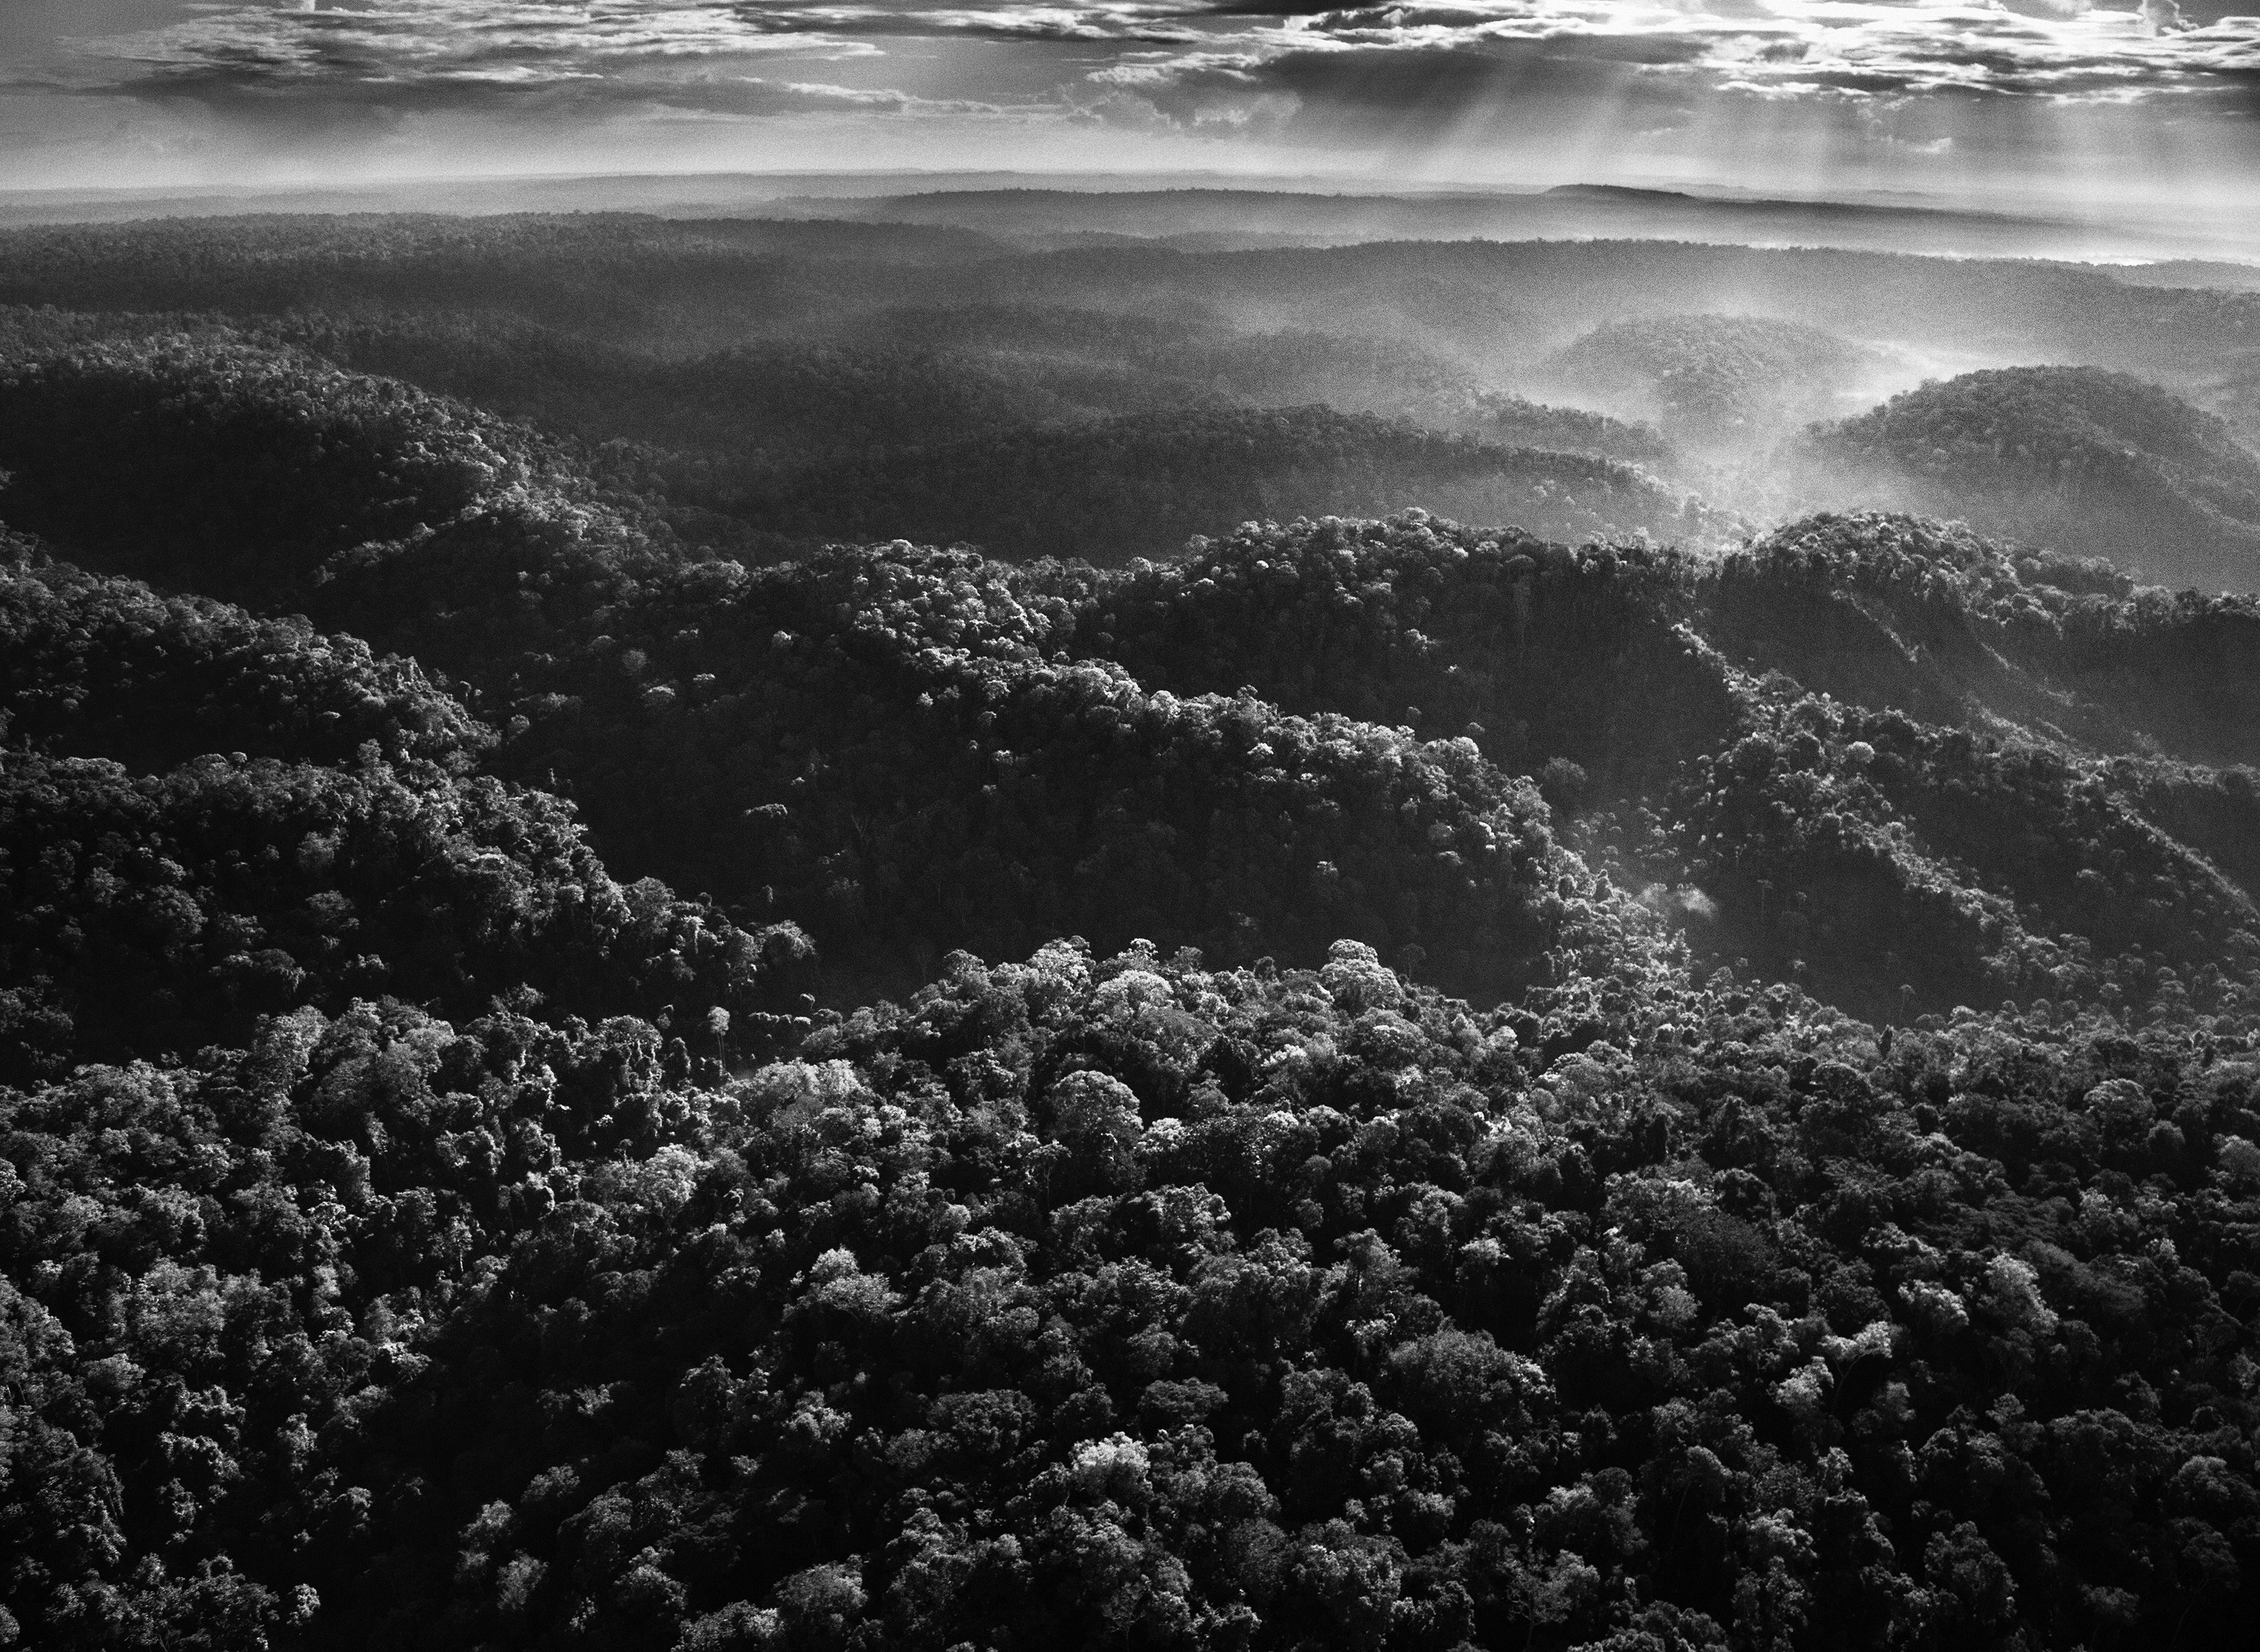
\includegraphics[width=\textwidth]{./imgs/Paisagem_SS}
%\caption{\textit{Wytyra} ou as serras, morros e ladeiras entre as Terras Indígenas Awá e Caru (Foto aérea de Sebastião Salgado/Amazonas Imagens, 2013).}
%\end{figure}

As narrativas do contato passam pela introdução de novos alimentos e a
mudança na dieta. \textit{Saber comer} alimentos como farinha ou frangos era
algo que os Guajá desconheciam, e como veremos no decorrer desse livro,
alimentos outrora restritos passaram a ser consumidos com mais
frequência enquanto outros deixaram de sê-lo. Mesmo durante os anos de
fuga, no \textit{tempo do mato}, procuravam permanecer
próximos aos cursos dos rios, o que nem sempre era possível. Tinham que
viver nas ``montanhas'', \textit{wytyra}, onde não há água, e quando
precisavam tomar banho ou pegar água desciam as grandes encostas que os
mantinham seguros, usavam o igarapé mais próximo e retornavam às
``terras altas'', \textit{wytyra}. Dentre tantos, o principal desconforto
em viver longe de uma fonte de água no meio da floresta era a sede que
experimentavam nesses anos. Esse \textit{tempo da sede},\footnote{ \textit{Haiwe},
``minha sede''.} que como lembram era uma ``sede intensa'', \textit{iwe
rahy}, caracteriza os \textit{anos de fuga}, rememorados como \textit{wyhy
ka'a ripi}, ``correndo pelo mato''. Nesse tempo, as caçadas eram
difíceis, e para não chamar tanta atenção passaram a ser realizadas à
noite.\footnote{Como veremos no capítulo 8, no que concerne à caça de
macacos, é algo de extrema dificuldade se for realizado sem luz.} Essa
vida nas \textit{terras altas} me foi relatada da seguinte maneira por
Akamatỹa:

\begin{quote}
Nós sempre fugíamos subindo pela montanha. Matávamos capelão e
corríamos para lá. Certa vez, os \textit{karai} estavam correndo
atrás da gente e nós conseguimos matar apenas um capelão. O capelão
ficou lá em cima da árvore e o matamos à noite, escondido, para os \textit{karai}
não nos verem. Esperamos lá em cima da montanha e à noite voltamos para
matar capelão escondido. Não tínhamos mais comida, a cabeça doía, e
pensávamos que tínhamos que comer capelão. Os \textit{karai} nos perseguiam e
tínhamos que ficar fugindo para a montanha. Vimos o rastro dos \textit{karai} 
e fugimos de novo. Quando descíamos, ficávamos só um
pouco e logo tínhamos de fugir de novo. Pensávamos: \textit{como vamos viver
assim?} Minha mãe, grávida, perdeu um filho porque fez muito esforço,
correndo {[}pelas terras altas{]}, e ficou com muito medo. Descemos para
procurar babaçu no cocal e ficamos de novo só um pouquinho. Depois,
fugimos para a montanha. Queríamos muito comer babaçu, mas os \textit{karai}
estavam lá, nos procurando. Não tínhamos nada para comer. Ficamos lá
escondidos por muito tempo, com sede, com fome e queríamos voltar. Mas
os \textit{karai} estavam lá. Minha mãe ficava muito preocupada: \textit{como vamos viver
assim?} \textit{Vamos tentar ficar aqui escondidos mais um pouquinho}, ela dizia.
Eu, que era seu filho, saía de lá para ver se dava para descermos da
montanha, mas encontrava rastro dos \textit{karai}. Ficávamos sempre fugindo, e
os \textit{karai} sempre correndo atrás de nós. Minha mãe me falava: \textit{como vamos
viver assim?} E eu falava: \textit{não sei, mãe}! Ela dizia, então: \textit{vamos ficar
aqui escondidos mais um pouquinho}. E ficávamos em cima da montanha, sem
conseguir sair para caçar ou comer babaçu.
\end{quote}

Nessa época, quando as \textit{terras altas} lhes traziam um pouco de
segurança, eram ``gente do mato'', \textit{awa ka'apahara}, e não conheciam
o jeito dos \textit{karai}. Algumas pessoas queriam aparecer
para o contato com os \textit{karai} enquanto outros resistiam, pois
tinham medo, como certa vez me explicou Kamairua. Não por acaso, é por
meio deste mesmo nome, \textit{awa ka'apahara}, ``gente do mato'', que os
Guajá que vivem nas aldeias pensam os pequenos grupos que ainda vivem
sem contato oficial.\footnote{Os \textit{isolados}, de acordo com a terminologia
vigente.} Como veremos no decorrer deste livro, essa vida de fuga e
abstinência é experimentada hoje pelos que se encontram isolados, pois
permanecem como \textit{gente do mato} e se alimentam
com uma \textit{comida de gente do mato}\footnote{ \textit{Awa mihu nimi'ũa}, ``comida
de gente braba''.} que as pessoas da aldeia há muito deixaram de
consumir, como o cará-do-mato, \textit{karuhua}, além de um
tubérculo chamado \textit{mara'atỹa}.\footnote{Não consegui identificá-lo. É 
glosado genericamente como \textit{raiz} ou \textit{batata do mato}.} Esses víveres
eram utilizados como alternativa alimentar durante as fugas. Destaco o
trecho de um depoimento gravado com Kamairua, na aldeia Tiracambu, em que
ele relaciona o consumo desse tubérculo à vida nas ladeiras e montanhas, à
falta de cônjuges e à penúria dos anos de fuga:

\begin{quote}
{[}\ldots{}{]} E estávamos fugindo dos \textit{karai}\footnote{Não indígenas.} e não
sabíamos o que comer. Não tinha caça. \textit{O que será que vamos comer?},
pensávamos. Vamos comer \textit{mara'atỹa}. E então comemos \textit{mara'atỹa}. Arrancamos
e comemos, apesar de ela ser uma raiz muito dura, que dá na montanha.
Nessa época, não tinha mulher para casar, não tinha rede. As redes
estragaram e não tinha mais fibra de tucum. Conseguimos um dia matar
capelão e comemos com \textit{mara'atỹa}.\footnote{Conversa com Kamairua, da aldeia
Tiracambu, 2013. Tradução de Uirá Garcia e Marina Magalhães.}
\end{quote}

Ainda sobre a vida em fuga pelas terras altas, Akamatỹa reflete sobre a
penúria alimentar e o \textit{mara'atỹa} em seus anos de fuga:

\begin{quote}
{[}\ldots{}{]} Comíamos só jaboti. Estávamos eu, minha mãe, meu pai e
minha irmã Pakawãja ainda bebê. Hajkaramykỹ ainda não tinha nascido.
Passamos a comer \textit{mara'atỹa}. Arrancávamos escondido
e comíamos assado. Mas um dia os \textit{karai} viram a fumaça e nos encontraram
novamente. Mandaram cachorro atrás de nós e tivemos de subir a ladeira
de novo e comer \textit{mara'atỹa} escondido. Queríamos muito comer babaçu, mas
os \textit{karai} não deixavam chegarmos ao cocal. Só podíamos comer \textit{mara'atỹa}
mesmo. Um dia encontramos um outro Awá-Guajá que perguntou para nós o
que estávamos comendo, falamos que só comíamos \textit{mara'atỹa} por causa da
fuga. Juntamos os grupos, ficamos juntos.\footnote{Conversa com Akamatỹa,
aldeia Tiracambu, 2013. Tradução: Uirá Garcia e Marina Magalhães.}
\end{quote}

Tal época foi marcada tanto pela dispersão quanto a
reunião de pequenos grupos que outrora se encontravam distantes no
território. Os Guajá tiveram que encontrar estratégias de alianças\footnote{\textit{Ruku}, ``estar com'' ou ``casar''.} e criação de filhos\footnote{\textit{Ixa'á}, ``crescer''.} para dar conta do grande número de crianças que se tornaram
órfãs devido à morte dos pais por doenças ou assassinato pelos
\textit{karai}\footnote{Sobretudo durante a década de 1970, quando a região foi
maciçamente ocupada.} ou que simplesmente eram deixadas para outros
parentes criarem. Xiramua, por exemplo, foi encontrado sozinho na mata, sem pai ou mãe, ainda criança, 
por um grupo liderado por Ximira, cujos parentes viviam nas cabeceiras do
Igarapé do Presídio e fizeram contato entre 1981 e 1983 (Garcia, 2013,
p.\,51). De acordo com um relato de Tatuxa'a, da aldeia Awá, seu pai,
Ximira, encontrou uma criança ainda tão pequena que não sabia falar,
sozinha na mata. Essa criança era Xiramua, cujos pais haviam sido
assassinados por \textit{karai}. Em outro relato,
Akamatỹa, da aldeia Tiracambu, relembra que seu pai ficou para trás,
deixando os filhos:

\begin{quote}
Antes de chegar aqui, meu pai ficou velho e disse: \textit{podem correr
na frente, meus filhos}. \textit{Estou velho e não aguento mais. Pode deixar que
me matem}. E ele ficou no mato. Uma vez eu pisei de noite em uma
surucucu, que me mordeu. Depois que chegamos aqui nessa região, tentamos
voltar de novo para o nosso antigo lugar, mas já não havia mais mata, só
capoeira.\footnote{Relato de Akamatỹa.}
\end{quote}

Kamairua, que também foi criado sem os pais, reforça os muitos
rearranjos de paternidade que visam à criação de crianças largadas, nos anos de fuga. A partir de si e seu amigo, Irakatakoa, ele revela:

\begin{quote}
Antigamente eu vivia no mato. Eu não conheci meu pai e ficava
com minha avó, Mirakexa'a. Da mesma forma que Irakatakoa, que era bebê, e foi criado por Marakanã. Tínhamos medo dos \textit{karai}.
Irakatakoa nasceu, e sua mãe morreu de parto. Iam deixá-lo para que os
\textit{karai} o criassem, mas ficaram com pena, e Marakanã passou a criá-lo.
Quanto a mim, quando eu era pequeno, uns \textit{karai} chegaram e minha avó me
pegou, fugindo deles. Nós vivíamos juntos até que encontramos os \textit{karai} e
tivemos que nos espalhar{[}\ldots{}{]} Queríamos vir para cá,\footnote{Para o Posto
Indígena Awá.} mas tínhamos medo. Então ficávamos no mato, matando
capelão, queixada; moqueávamos queixada, comíamos. Piramỹna, então, se
separou de nós e eu fiquei com minha avó, Mirakexa'a, e Karawaxa'a. Foi
quando os \textit{karai} apareceram e tivemos de fugir. Minha avó
me pegou, pois eu era bem pequeno, e o meu pai fugiu para outro lado, em
direção ao Turiaçu. Por isso eu não conheci meu pai. Só fui conhecê-lo
há pouco tempo, lá no Turiaçu.\footnote{Na aldeia Guajá.} Eu vi meu pai, Tõja
{[}Kamixaxa'a{]}, depois de adulto. Eu era pequenininho, e foi minha avó
quem me criou. Eu comia ovo de jaboti, eu comia mel, lá na região do
Tabocão. E assim fui crescendo, crescendo até ficar grande.\footnote{Conversa
com Kamairua, 2013. Tradução: Uirá Garcia e Marina Magalhães.}
\end{quote}

A melancolia dessas lembranças remete aos muitos parentes que morreram,
ao medo dos brancos, à sede e à fome, além das cercas de arame farpado que
entrecortavam a terra e delimitavam fazendas, cujos jagunços\footnote{ \textit{Karai mihua}, ``brancos violentos''.} realizavam expedições
\textit{punitivas}, matando famílias inteiras. As feridas por arame farpado
colocados como emboscadas para machucar os Guajá, como Kamairu me
explicou certa vez, aparecem sensivelmente documentadas no filme
\textit{Serras da desordem}, de Andrea Tonacci. Xiramukũ, filho de
Karapirú, nasceu no mato e se separou da família em uma dessas
fugas após um ataque a tiros a seu grupo. Feito pelos \textit{karai} na
região de Porto Franco, Maranhão, em 1978, foi encontrado por moradores
locais preso a uma armadilha de arame farpado feita pelos próprios
jagunços que mataram sua família, por ordem do dono de uma fazenda da
região (Tonacci, 2006). Os Guajá, que viviam caminhando e nessa época
corriam em fuga, passaram a encontrar em suas trilhas\textit{\textit{Hapea}
``meu caminho''.} esse novo obstáculo, o arame farpado, colocado para
feri-los e, como no caso de Xiramukũ, prendê-los.

Em outra conversa, Irakatakoa e Xipowaha se lembravam de algo não tão
raro na história guajá, que era o encontro com colonos da região que
lhes forneciam utensílios, comida e outros artigos. Há uma história de
contato não oficial, bem anterior ao contato com a Funai, e de acordo
com relatos\footnote{Cf. Ribeiro, 1996; Beghin, 1957.} e depoimentos, como a
narrativa que abre este livro, esses encontros eram menos \textit{traumáticos}.
Mais próximo de um interesse mútuo entre os Guajá e os moradores que viviam
isolados no interior da mata, derrubando a floresta para \textit{botar} roça,
no clássico modelo de derrubada, queima e povoamento que marca a
ocupação do Maranhão e de boa parte da Amazônia. Os ocupantes que não
entravam em conflito com os Guajá são lembrados como \textit{karai katy}, ``não indígenas calmos ou bons'', em oposição a, por exemplo, \textit{karai mihua}, os ``nervosos ou maus''. A própria Funai, à época dos
primeiros contatos, era considerada um tipo de \textit{karai katy} por ofertar utensílios e atrai-los.

\section{\textit{trabaio}, «trabalho»}

Se no \textit{tempo do mato} a dieta era marcada por uma espécie de
subalimentação e caçadas precárias, a chegada dos \textit{karai} mudaria
radicalmente o conteúdo e formas alimentares. A introdução de espécies
cultivadas seria o principal decodificador dessa passagem de \textit{awa
ka'apahara}, ``gente do mato''\footnote{ \textit{Awa mihua}, ``gente braba''.} para \textit{awa katy}, ``gente mansa'' ou ``gente da aldeia'', tal como
se pensam hoje em dia. O espanto, receio e curiosidade frente a esses
novos alimentos é refletido por Irakatakoa, da aldeia Awá, que se
lembra inclusive de Mércio Gomes,\footnote{Antropólogo e ex-presidente da Funai, trabalhou com a antiga Frente de Atração.} durante o contato com
seu grupo, realizado na região do Igarapé Timbira, entre 1980 e 1983:

\begin{quote}
Eu era pequeno. Mas meu pai, Tatajkamaha, conta que Mércio
{[}chamado aqui de Jakuxa'a{]} ofereceu arroz para ele dizendo que era muito
gostoso. Meu pai experimentou e cuspiu. Achou muito ruim e ficou bravo
com ele. Aí ele disse que era para meu pai ficar calmo, pois ele era um
\textit{karai katy}, ``branco bom''{[}\ldots{}{]} Ele ia nos levar para lá {[}\textsc{pin} Awá{]}
para nos amansar, para aprender a comer sal, açúcar e café. E meu pai
experimentava e cuspia, jogava tudo fora. Aí um dia, o Piramỹna
experimentou e gostou. E Mércio disse que íamos nos acostumar e que ia
ficar tudo bem conosco lá. Ia ter arroz, feijão, abóbora, cebola. Mas
tudo o que provávamos, jogávamos fora. E nos escondíamos novamente no
mato. Aí o Major ia atrás de novo. Alguns de nós %(apelido de um antigo)
ficavam tremendo de medo. E ele dizia: --- Não vamos te matar não,
queremos que vocês se acostumem conosco. Eu também tinha muito medo.
Chorava e fazia cocô. Porque eu não conhecia branco. Aí Mércio disse que
seria bom pra mim. Aí eu fiquei acostumado e vim para cá, com todos os
outros. Já estavam aqui o Ximira e o Urixia. Eles já tinham nos avisado
que teriam outros Awá-Guajá aqui também. Estavam também o Mitũa, o
Kamana'ĩa. E minha avó {[}a falecida Mirakexa'a{]}, que veio conosco, já
conhecia\footnote{De uma época anterior ao contato.} eles todos.\footnote{Conversa com
Irakatakôa, da aldeia Awá, 2013. Tradução de Uirá Garcia e Marina Magalhães.}
\end{quote}

Os relatórios da Frente de Atração reportam sobre a compra de farinha de
mandioca a ser fornecida aos grupos contatados na década de 1980, algo
que logo se tornou insustentável, obrigando as aldeias que se formaram a
produzir a própria farinha em um regime de trabalho coordenado pela
Funai. Tal situação fez rapidamente com que a farinha de mandioca puba se
tornasse a base da dieta.

Em todas as jornadas de caça, a farinha é um item essencial. Não existem
caçadas sem que se leve ao menos uma pequena quantidade de farinha para a
floresta. Quando estão em seus acampamentos de caça por muitos dias ou
semanas, sempre haverá alguém na aldeia torrando mais farinha para ser
levada ao acampamento. Na alimentação cotidiana isso também é sentido.
Os Awá adicionam farinha a praticamente todos os alimentos que consomem: abóbora, coco de babaçu, inajá, bacaba e açaí. Além disso, é usada para fazer mingaus a partir dos caldos de carnes, peixes e legumes. O
reflexo desta não intimidade com o trabalho agrícola, bem diferente de
seus vizinhos Ka'apor e Guajajara, pode ser visto, por exemplo, na
falta de assiduidade com que os Guajá mantêm suas roças, muitas das quais
têm a colheita seriamente prejudicada. De acordo com Forline:

\begin{quote}
As roças normalmente exigem um ciclo de atividades que tem que ser
seguido conforme o calendário metereológico e ecológico. Isso implica na
limpeza, derrubada, queima, coivara, plantio, colheita e capinagem.
Segundo estimativas de alguns funcionários da Funai, os Guajá não têm um
aproveitamento total ou máximo de suas roças, perdendo até 60\% de sua
produção, dado que ainda não têm a experiência que seus vizinhos possuem
na agricultura e ainda dedicam mais tempo de suas atividades produtivas
à caça, situação essa que não antecipa muito a sucessão florestal e o
avanço das capoeiras.\footnote{Forline, 2007, p.\,6.}
\end{quote}

Em suma, mesmo havendo hoje em dia o cultivo agrícola nas aldeias com 
a ajuda de mão de obra contratada pela Funai, ainda não
podemos afirmar que os Awá sejam algo como \textit{horticultores}, no
sentido que a ecologia política atribui a essa ideia, embora seja
possível identificar um processo de incorporação da agricultura à vida.
A lógica de ação é baseada na caça, e todos ainda estão dispostos a
trocar uma colheita pela floresta, a partir de uma
mera suspeita da existência de uma vara de porcos ou um bando de
capelães.

Com isso, deparamo-nos com uma \textit{missão civilizadora} por parte do
órgão indigenista para transmitir ou ensinar o trabalho agrícola aos
Guajá. Até os dias atuais, observa-se na fala de funcionários da Funai
que convivem diretamente com eles a preocupação que norteou os anos de
contato, e que permeia inclusive as políticas de contato atual: o medo de os grupos 
recém-contatados morrerem por inanição ao se recusarem a consumir os alimentos 
introduzidos pelos brancos, já que há dificuldade em manter a antiga dieta, 
do \textit{tempo do mato}. Assim, na época da Frente de Atração, até a década de 1990, o posto indígena
tornou-se uma espécie de unidade produtiva, mantendo com as aldeias uma
relação que passava fundamentalmente por comando e ordem, tal qual uma
\textit{colônia agrícola} ou algo do gênero, cujos resquícios são sentidos
até os dias atuais.\footnote{Sugiro aqui que tal relação possa ser pensada a
partir da ideia de \textit{trabalho}, tal como observa-se há décadas pelos
funcionários da Funai, a partir de ideias como \textit{os índios
precisam aprender a trabalhar}, ou \textit{os índios não sabem
trabalhar}, ou mesmo que \textit{se não trabalharem, esses índios vão
morrer de fome}.} 

A figura do \textit{trabalho}, tal como coordenado pela
Funai, com contratação de mão de obra de moradores do entorno da terra
indígena para ajudá-los, é traduzida pelos Guajá mediante a ideia de
\textit{trabaio}, que, como experimentei na aldeia Juriti onde vivi
durante o meu doutorado, pode ser considerada algo diferente de
\textit{trabalho}. Por exemplo, pronunciar palavrões em português, soltar
gritos e um monte de jargões do tipo \textit{eu sou trabalhador}! ou
\textit{eu sou duro}!, dentre outros, compõe uma sociabilidade
masculina experimentada no trabalho de roça dos \textit{karai} e
atualizada pelos Guajá a partir da ideia de \textit{trabaio}.\footnote{Eu mesmo
passei excelentes momentos junto aos homens nessas atividades que
misturam a alegria de estarem juntos com seus amigos e com os
\textit{karai katy}, os ``brancos bons'', da Funai, momentos em
que visivelmente os Guajá imitavam de muitas formas os \textit{karai},
tentando entender um pouco mais sobre eles.}

Um conjunto de elementos e ações define o \textit{trabaio}\footnote{Ou
\textit{trapaio}, a depender da pronúncia.} que ocorre fundamentalmente na
lavoura. Para ir à roça, um homem, além de ferramentas como facões e
terçados, exige roupas: calça comprida, botina, boné e camisa de manga
longa para se proteger; o mesmo tipo de vestimenta que os \textit{karai} 
utilizam no trabalho na roça. Vestir roupas de branco faz
parte do \textit{trabaio} da mesma forma que beber a água gelada do posto
da Funai levada pelos funcionários para a roça, perguntar e comentar
detalhes íntimos da vida em casal em tom de provocação, e,
principalmente, consumir a comida dos \textit{karai}.\footnote{Em uma conversa que
tive com Irakatakoa, da aldeia Awá, ele afirma precisar comer a
``comida do branco'', \textit{karai nimi'ũa}, arroz, macarrão, carnes e
sardinhas em lata, quando vai para a roça: ``É assim que os
brancos trabalham na roça. Suas mulheres preparam a comida e os homens
levam a comida para a roça, por isso é assim que deve ser o trabalho dos
Guajá. Com comida nós vamos para a roça''.} 

Na tentativa de estimular
atividades de roça para os Guajá da \textsc{ti} Caru, a Frente de Proteção
cogitou inclusive pagar uma espécie de bônus por cada linha de
roça\footnote{No estado do Maranhão, as roças são medidas por \textit{linhas}, e cada uma equivale a 0,30 hectare.} cultivada, além de se encarregar
de levar o \textit{rancho} a cada jornada na lavoura.

A política oficial atual é não oferecer mais nada do que se oferecia
nas décadas anteriores: farinha, sal, sabão, munição etc. Pouca coisa
mudou, e a procurada autonomia para o \textit{trabalho} não vem
ocorrendo como se esperava no passado. É comum os funcionários da Funai
reclamarem da dificuldade em \textit{juntar três ou quatro homens para o
trabalho}. Por exemplo, em 2012, a grande aldeia ligada ao posto
indígena Awá, por falta de comunicação e organização desses
trabalhos não fez nenhuma roça, e em 2013 foi necessário que a própria
Funai comprasse toneladas de farinha e partes cultivadas por
agricultores próximos para dar conta das necessidades da aldeia. No
entanto, esse descompasso que ainda existe na vida das pessoas, como
veremos, se deve à diferença de estatuto entre a caça e a ``comida de
gente'', \textit{awa nimi'ũa}, além da ``comida dos não indígenas'', \textit{karai
nimi'ũa}. 

Os Guajá reclamam que seus filhos e mulheres têm fome, que
precisam caçar para eles, e que quando vão para a roça não conseguem
efetivamente fazê-lo. Não à toa, são capazes de quebrar qualquer acordo
prévio que tenham feito com os funcionários do posto indígena e de
trocar a lavoura por uma promessa de caça, seja por alguém ter
encontrado um rastro ou serem informados por um sonho, ou mesmo para
suprir o desejo de uma mulher, um filho ou até um sogro, para desespero
dos servidores que os arregimentavam para o trabalho e encontram nesses
momentos um sinal da própria \textit{inconstância} Guajá. Ir para a roça
nesses casos é, antes de tudo, sinônimo de não ir caçar.

A floresta, por sua vez, seria o oposto do \textit{trabaio}. Fresca e
cheia de imprevisibilidade, ela se distingue frontalmente das aldeias e
roças, locais quentes e monótonos se comparados a ela. Acostumados
à vida no interior da mata, sempre ``fresca'', \textit{haxỹ}, a
exposição ao sol por muitas horas é algo considerado bastante
desagradável. Um dos componentes, portanto, que agenciaria essa ideia de
\textit{trabaio} passa pela possibilidade de suportarem o calor do sol, o \textit{kwarahy haku}. 
Ser ``forte'', \textit{hatỹ}, no trabalho
significa aguentar o trabalho de sol a sol, tal como valorizado pelos
\textit{karai} e anteriormente desprezado pelos Guajá. É comum
ouvirmos de uma aldeia para outra que naquele local eles sabem trabalhar
pois são mais \textit{duros} e seus corpos aguentam o sol, diferente de
outras aldeias onde as pessoas ainda seriam \textit{selvagens}\footnote{ \textit{Awa ka'apahara}, ``gente do mato''.} e moles para o trabalho.

Podemos pensar que \textit{trabalho} aqui seria mais uma daquelas noções como
\textit{dinheiro}, \textit{desenvolvimento}, \textit{lucro}, \textit{produção}, \textit{higiene},
\textit{educação}, \textit{lazer}, \textit{alma}, dentre tantas outras levadas aos
povos não ocidentais a partir do aparelho colonial, ao mesmo tempo que
reviradas e repensadas pelos mesmos.\footnote{Sahlins, 1997, Wagner, 1981, pp.
31--33.} Parafraseando a ideia melanésia de \textit{divelopman},
desenvolvida pelos Agamen da Nova Guiné,\footnote{Nihil, 1989 \textit{apud} Sahlins, 1997\,\textsc{a},
p.\,59.} \textit{trabaio} é um conceito amplo entre os Guajá, avaliado
sobretudo a partir das mudanças experimentadas na passagem de um tipo de
\textit{gente da floresta} para outro tipo de \textit{gente mansa}.
\textit{Trabaio} aqui seria a tradução de um estilo de vida, e não apenas
\textit{trabalhar}. Sem dúvida, o \textit{trabalho} também é contemplado por essa
ideia, que sugere algo mais do que \textit{trabalhar}, traduzindo o próprio
jeito de viver dos não indígenas.\footnote{Quando eu estava em casa
e demorava para retornar à aldeia Juriti, meus amigos sabiam tratar-se de
\textit{trabaio}, que incluía também andar de avião, dirigir automóveis,
cuidar de uma família com mulher e filhos, comer comida de branco,
enfim, viver como um autêntico \textit{karai}.}

De alguma forma o \textit{trabaio} é tudo o que os Guajá não
experimentavam antes do contato, e toda transformação vivida
recentemente pelas pessoas das aldeias, interessadas agora em dinheiro,
escola, carteira de motorista, dentre outros serviços e bens
estrangeiros, passa pela ideia de que os \textit{karai} 
\textit{trabalham} para terem essas coisas, ao passo que os Guajá ainda não
saberiam \textit{trabalhar} --- na roça, por exemplo. Ao menos na aldeia
Juriti, o \textit{trabaio} é também um compromisso de atividades com a
Funai que os restringiria em sua vida na floresta. 

Para as pessoas dessa
aldeia não se trata apenas de \textit{trabalhar} nas roças, pomares e áreas
onde é preciso capinar, como orientam os funcionários do posto, o
\textit{trabaio} engloba um conjunto de problemas, dilemas e diferenças
que pautam a própria relação entre os Guajá e os brancos. O conhecimento
que temos das máquinas, o desprezo que temos pela floresta e pelos
conhecimentos indígenas, a brutalidade e grosseria presentes nas
relações entre amigos do sexo masculino --- algo deveras chocante para os
homens Guajá ---, a divisão do tempo, a dieta, o mundo do dinheiro, enfim,
é a própria vida dos \textit{karai} ou \textit{sociedade}, 
que é traduzida pela ideia de \textit{trabaio}. Algo como o \textit{kago}
melanésio,\footnote{Wagner, 1981, p.\,31.} \textit{trabaio} seria a contraparte Guajá
para ideias como \textit{qualidade de vida} ou mesmo \textit{cultura}.
\textit{Trabaio} é a palavra \textit{neoguajá} para a experiência de
\textit{virar branco} (Kelly, 2005) que revela ``um processo --- um momento
passageiro de \textit{primeiro contato} que pode bem durar mais de cem anos''
(Sahlins, 1997, p.\,60). Parafraseando Roy Wagner, \textit{trabaio}
funcionaria como \textit{um termo de mediação entre diferentes povos}, e \textit{a
relação que ele encarna} torna-se aquela dos Guajá com a sociedade
nacional e com o próprio Ocidente (Wagner, 1981, p.\,32).


\chapter{Habitar}

%\begin{figure}[H]
%\centering
%  \includegraphics[width=\textwidth]{./imgs/IMG_2922}
%\caption{(da esquerda para a direita) Jakara'yra, Makarikarỹa, Takwaripijua e Kamajrua (agachado) colhendo juçaras na época das chuvas (aldeia Tiracambu, 2013).}
%\end{figure}

\section{palmeiras selvagens}

\noindent{}Dentre as etnografias que abordam a organização espacial de povos
amazônicos que encontram na caça uma atividade central, sejam
horticultores ou não,\footnote{Ver, por exemplo, o balanço de Rival, 1999.} uma
das alegorias mais comuns é a do território como um espaço marcado por
histórias de caçadas e guerras, uniões matrimoniais e cisões entre
afins, nas quais os saberes produzidos nas interações com a floresta
seriam, todo o tempo, colocados à prova e reinventados. Desde a paisagem 
supostamente caótica das florestas do Capauari, tão
familiares aos Ashuar, um \textit{território varado por mil acontecimentos}
que fornecem à paisagem aparentemente anônima sua devida substância
histórica\footnote{Descola, 2006, pp.\,153--154.}, passando pelos muitos 
topônimos existentes no léxico parakanã para situá-los em suas trilhas, e pelos quais se
localizavam durante seus períodos de \textit{trekking},\footnote{Fausto, 2001, p.
105.} até o interesse dos Huaorani em sempre seguir adiante, por seus
caminhos, acompanhando o florescimento dos vegetais e o movimento dos
animais.\footnote{Rival, 2002, p.\,68.} Também o \textit{seminomadismo} sirionó que, 
através dos \textit{ñenda}, os ``caminhos de caça'', descobrem a cada caminhada uma
nova floresta que lhes fornecerá as aldeias-acampamentos em que vivem,\footnote{Holmberg, 1969, p.\,105.} 
e a cultura material \textit{descartável} dos nômades
Yuquí, donde os poucos objetos fabricados, como cordas e cestos, são feitos e
refeitos de acordo com a necessidade, subprodutos exclusivos de sua bem
sucedida relação com a floresta.\footnote{Stearman, 2001, p.\,41.} Não ficam de fora 
as complexas descrições sobre o território realizadas pelos Akuriyó, levando-se em
conta, fundamentalmente, a vegetação e a fauna, que coincidem com as
descrições presentes \textit{nas melhores enciclopédias de fauna e flora} já
produzidas sobre o norte amazônico.\footnote{Jara, 1996, p.\,96.} Enfim, em
variados contextos etnográficos sul-americanos, entre povos para os
quais a caça desempenha um papel fundamental, que enfatiza um permanente
estar em movimento na floresta, a produção de múltiplos significados
sobre o território é condição primordial à existência da vida. São
espaços \textit{culturalizados}, nos termos de Ingold, cujas relações são,
antes, entre pessoas encarnadas em formas orgânicas, frágeis e não
permanentes,\footnote{Ingold, 2000, p.\,53.} e nestes espaços a história está
escrita.\footnote{No capítulo que segue, apresento as formas pelas quais os Guajá concebem
e arranjam aquele que é seu lugar de vida: a floresta, \textit{ka'a}.
Para tanto, discuto a ideia de \textit{harakwaha}, termo que abrange tanto
o domínio territorial quanto as relações envolvidas no território. Ao
final do capítulo, apresento um pequeno esboço sobre a cosmografia
Guajá.}

Como apresentei no capítulo anterior, os Guajá não têm uma economia
hortícola. Milho e mandioca foram introduzidos após o contato com o
Estado brasileiro, e nenhum dos subprodutos de uma \textit{agricultura
tradicional} indígena, como fumo, beiju e bebidas fermentadas, tal
como encontramos em outros povos amazônicos, como os horticultores Tupi, 
poderá ser encontrado entre os Guajá. Os espaços de vida
que constituem o território Guajá não contemplam a consagrada
espacialidade tupi, e amazônica, de uma forma geral, que opõe a roça e
a mata como espaços-eventos complementares em um ciclo sazonal. Como na
maioria dos grupos Tupi-Guarani, o eixo céu-Terra é um dos aspectos
fundamentais para entendermos a forma com que os Guajá se movimentam no
espaço.\footnote{Há exceções, como é o caso dos Waiãpi (Gallois, 1988).}
\textit{Iwa}, \textit{haripa} e \textit{ka'a} --- ``céu'', ``aldeia'' e ``floresta'',
respectivamente --- são talvez os principais centros em torno dos quais a
vida gravita, formando pares particulares como ``céu-Terra'';
``Terra-mata''; ``mata-céu'', que veremos daqui em diante. Céu e mata são
domínios pelos quais os Guajá guardam grandes interesses. Em boa parte
das conversas figuram como tema central, e eu não saberia afirmar sobre
qual as pessoas mais elaboram. A floresta, \textit{ka'a}, é o local em que
sempre viveram, \textit{habitat} de tudo o que conhecem: animais, mel,
remédios. Apesar de todo o perigo que oferece, é o local que durante
sua história recente lhes forneceu a segurança e a distância necessária
dos \textit{kamara} e \textit{karai} --- os ``outros indígenas'' e os
``não indígenas'', respectivamente. Se não vivem mais baseados em
acampamentos, dormindo em tapiris como antes, não dispensam a vida na
floresta, local \textit{haxỹ},``fresco'', e \textit{parahỹ}, ``bonito'', 
diferente da aldeia, que dizem ser \textit{haku},``quente''. e \textit{manahỹ}, ``desagradável''. 
Principalmente no verão, a aldeia do posto é utilizada como base para novas incursões
de caça, e a caça é um dos principais assuntos tratados no dia a dia da
aldeia: munição, locais de caça, rastros de animais, etc., são os temas
que mais interessam. Os fatos da vida quase sempre são fatos da caça.

O \textit{haripa}, ``minha casa'' ou ``minha aldeia'', nos dias atuais,
difere do que era antes do contato. Enquanto no passado os grupos
locais, formados por uma ou algumas famílias, viviam em aldeias
provisórias ou semipermanentes, refeitas devido aos deslocamentos
constantes dos grupos nos dias atuais, o que vemos são conglomerados de
antigos grupos locais que depois de amontoados se transfiguraram no
formato \textit{aldeia permanente}, devido tanto à proximidade com o posto da
Funai, que dispõe de bens e serviços, quanto ao maior conforto oferecido
por esta conformação espacial, sobretudo na época das chuvas. Os
pequenos acampamentos, próximos a áreas com grande oferta de caça e
frutos, deram lugar a grandes clareiras, com dezenas de casas onde vivem
até 180 pessoas --- como no caso da aldeia Awá, cada vez mais
distantes das áreas de caça. No entanto, por não se interessarem em
manter uma vida de cultivo nas roças, precisam voltar diariamente ao
mesmo interior da floresta onde outrora viviam. Andam para cada vez mais
longe, para onde a caça se foi, e precisam retornar à aldeia do posto,
tudo isso em uma única jornada. As aldeias, tal como hoje estão
organizadas, são espaços por um lado monótonos, dizem os Guajá, mas
dotados de vantagens, como a aludida proximidade com o mundo dos
\textit{karai}, e de uma estrutura fixa e funcional que os desobriga de
montar e desmontar seus acampamentos a cada poucos dias ou semanas. A
caça, por sua vez, devido ao desmatamento e à proximidade com os
brancos, está cada vez mais \textit{brava} e por isso, ao menos perto das
aldeias, locais de perturbação humana e barulhentos, mais difícil
caçar.

Como a grande maioria dos povos amazônicos, os Guajá não têm uma palavra
designativa para \textit{animal}; cada um é denominado por sua espécie, tipo,
tamanho ou outra característica. Na língua guajá, no entanto,
encontramos um termo para \textit{caça} ou \textit{presa} que pode ser traduzido
também por ``bicho'': \textit{ma'amiara}, ou simplesmente
\textit{ma'a}. A partir disso, fazem uma distinção
categórica entre ``caça brava'', \textit{haitema'a}, e ``caça mansa'', \textit{haite'yma'a}. 
Em linhas gerais, a \textit{caça brava} é aquela acostumada
com o barulho dos tratores, motosserras, povoados, estrada de ferro e
presença dos humanos. A \textit{caça brava} é mais atenta e desconfiada; conhece 
os humanos e, portanto, se torna mais difícil de caçar. Já a \textit{caça mansa} 
vive no interior da floresta, nas
áreas ainda preservadas. Nesses lugares, os animais estão menos
acostumados com a presença humana e vivem menos escondidos. Esses
\textit{santuários}, verdadeiras \textit{reservas de comida}, são ocupados durante
todo o ano, com mais intensidade na época seca, e é onde, como veremos, 
ainda se conseguem grandes quantidades de caça. As casas na
floresta, os acampamentos, são levantados nessas áreas, refúgio de
muitas espécies animais, longe das aldeias e dos postos indígenas. Lá, a
caça fica perto das casas e os acampamentos, além de existir em abundância.

%\section{seco e molhado}

\section{\textit{Tamỹkoa} e a origem do verão}

\begin{quote}
\textit{Tamỹkoa} era um sujeito que morava na floresta e tinha os pelos
muito compridos. Seus cabelos, \textit{jakyra}, e barba, \textit{jamatara},
eram tão longos que se arrastavam por muitos quilômetros pelo chão. Os
pelos pubianos, \textit{hajmõ kamỹtara}, eram tão compridos que
atravessavam a floresta inteira, bem como os das axilas, \textit{jaura}, onde cada um seguia a direção de um braço, indo em
direções opostas até os recônditos daquele mundo. Até mesmo os pelos do
seu ânus, \textit{hajkarapyra}, eram longuíssimos e sumiam pelos caminhos
da floresta. E os cabelos de \textit{Tamỹkoa} iam longe na floresta, cada
um em uma direção.

Nessa época, o herói cultural \textit{Maira}, o demiurgo que criou, dentre
tantas coisas, a própria humanidade, havia fugido junto com seu irmão
gêmeo \textit{Mukuxa'a}, o Gambá, da aldeia das onças onde foram criados
como filhos e prisioneiros ao mesmo tempo. As onças haviam comido sua
mãe quando os gêmeos eram bebês e, quando cresceu, \textit{Maira}, após
descobrir a traição, conseguiu matar em vingança algumas onças e fugir
com seu irmão, \textit{Mukuxa'a}, à procura de seu pai \textit{Mairua}.\footnote{Literalmente, ``o pai de \textit{Maira}:\textit{Mai}, de ``\textit{Maira}'', junto ao sufixo \textit{r-ua}, ``pai de''.} 
Após um tempo de procura, \textit{Maira} e
\textit{Mukuxa'a} encontraram o pai vivendo na floresta. O encontro, no
entanto, foi mal sucedido, com \textit{Maira} e \textit{Mukuxa'a} transformando o
arco do pai em cobra, e os quatis que \textit{Mairua} havia caçado, em pedra.\footnote{Voltarei à saga de \textit{Maira} no
  próximo capítulo.} O pai de \textit{Maira} ficou muito bravo com seus
filhos e decidiu abandoná-los, ou sair para caçar sozinho.

Nessa época, \textit{Tamỹkoa}, o sujeito de pelos compridos, vivia nesta
mesma floresta. Durante sua caminhada, \textit{Mairua}, o pai dos gêmeos,
o encontrou dormindo. Quando o avistou, pensou: \textit{Ah, Tamỹkoa
está aqui, dormindo!}. O pai de \textit{Maira} conseguiu passar por ele
sem acordá-lo, seguindo o seu caminho. Logo atrás de \textit{Mairua}
vinham seus filhos, \textit{Maira} e Gambá, que encontraram o rastro de
pelos de \textit{Tamỹkoa}. \textit{Maira} comentou com \textit{Mukuxa'a}, em
um falar sussurrado para não acordar \textit{Tamỹkoa}: \textit{Meu irmão,
Tamỹkoa está dormindo para lá. Vamos pôr fogo em seus pelos
compridos, o fogo vai alcançá-lo!}. E \textit{Maira} e seu irmão Gambá
puseram fogo nos pelos de \textit{Tamỹkoa}. \textit{Mairua} a essa hora
estava bem à frente no caminho, e não imaginava que seus gêmeos iriam
segui-lo, e muito menos atear fogo em \textit{Tamỹkoa}.

O corpo de \textit{Tamỹkoa} se encontrava longe, muito longe deles, mas
seus pelos e cabelos eram tão compridos que os gêmeos perversos podiam
lhe tocar fogo à uma grande distância, a muito tempo de caminhada. O
fogo se espalhou pelos pelos de \textit{Tamỹkoa} e percorreu a floresta
inteira, passando o incêndio de um pelo ao outro. Tudo se queimou, como
um interminável caminho de fogo que secou o mundo todo. O incêndio
também secou os rios menores e os igarapés.

\textit{Tamỹkoa} acordou sentindo um calor e, com a proximidade do fogo,
fugiu em desespero procurando algum curso d'água onde apagar o incêndio
de seus cabelos, mas estava tudo seco pois o fogo havia secado tudo.
Todos os seus pelos foram se queimando: o cabelo, os pelos das axilas,
pelos pubianos, do ânus, além da longa barba. Tudo foi queimado, e não
havia água para ele aliviar o incêndio. O incêndio secou a floresta.

Enquanto \textit{Tamỹkoa} queimava, \textit{Maira} e seu irmão, Gambá, riam sem
parar. Depois de tanto procurar, e quase morrendo, \textit{Tamỹkoa}
conseguiu encontrar um rio, para onde se jogou, e vive dentro d'água até
hoje; nunca mais voltou à floresta com medo de morrer queimado.
\textit{Tamỹkoa} parece gente, como os \textit{awa}, mas vive com sua gente
embaixo d'água. Dizem que na época seca, quando os rios secam,
\textit{Tamỹkoa} pode ser visto pois gosta de tomar um pouco de sol, mas
sempre retorna às águas. Devido a esse grande incêndio que varou o
mundo, provocado por \textit{Maira} e seu irmão \textit{Mukuxa'á}, e a
contragosto de seu pai, \textit{Mairua}, até hoje, durante boa parte do
ano esses pequenos cursos de rios e igarapés ficam secos.\footnote{Narrado por
Hajkaramyykỹ.}
\end{quote}

\begin{center}\adforn{68}\end{center}

A estação chuvosa se inicia no final de dezembro, com intensificação do
volume das águas em janeiro, chegando ao máximo da cheia nos meses de
abril e maio. Já a seca, que se inicia em junho, tem seu auge no
mês de outubro. O calendário é bem dividido em duas estações: o intervalo de dezembro a junho sendo \textit{inverno}, 
e julho a dezembro, \textit{verão}.\footnote{Para detalhes sobre o índice pluviométrico, dentre
  outros índices para as estações, ver Balée (1994, pp.\,9--10).} \textit{Sol}
e \textit{chuva}, é assim que os Guajá se referem às duas estações do ano: o
inverno é chamado \textit{amỹna ky mehẽ}, literalmente, ``quando a chuva
vai'', e o verão é \textit{kwarahy mehẽ}, ``quando tem sol''. E as pessoas
guardam sentimentos e percepções bem diferentes sobre cada uma delas.

Em uma tarde de março, no inverno de 2008, a chuva invadia a casa de
Wiraho. As folhas de babaçu, colocadas um ano antes e substituídas
apenas em alguns pontos, não eram suficientes para aplacar a força da
água. Embora o telhado conseguisse abrandar o vigor da chuva, tivemos
que recombinar nossas redes para que as goteiras da casa não tirassem
nosso conforto. Trovejava bastante. \textit{São os \textit{tapỹna}}!, me disse o
jovem Juwi'i. \textit{Estão com muita raiva}, \footnote{\textit{Imahy}, ``ele está com
raiva''.} \textit{eles sempre estão brabos}, disse-me o velho Pirama'ã,
antes de começar a entoar a canção de um \textit{karawara} chamado
\textit{Takwari} \textit{pini'ĩ}, uma ``gente-taquarinha'' que vive no céu,
cuja canção atemoriza os \textit{tapỹna}. Por isso, sempre que os
\textit{tapỹna} estão nervosos e na Terra se ouve o barulho de seus gritos,
os trovões \textit{tapỹna}, deve-se cantar: \textit{takwaaariiii}
\textit{pinĩĩĩĩ}, \textit{takwaaariiii} \textit{pinĩĩĩĩ}, até que os trovões
se acalmem. Se para de trovejar é sinal de que os \textit{tapỹna} ouviram
os humanos e se acalmaram. No moquém, \textit{pakapa'ã}, havia um pequeno
pedaço de cotia, \textit{akwixia}, que alguém caçara no dia anterior,
porém todos sentíamos alguma fome. Em meio a essa situação, com as redes
úmidas e os animaizinhos de criação encolhidos pelo frio de inverno, eu
conversava com Wiraho e Piraima'ã que me diziam que, com exceção do
aumento de gordura, \textit{ikira}, de muitos animais durante a época da
chuva --- o que é ótimo ---, preferem o verão, \textit{kwarahya}, quando não
sentem frio, podem andar livremente e dormem na mata.

Por ser no período chuvoso que grande parte das plantas frutifica,\footnote{\textit{A'e} \textit{ja'akera}, ``tem fruta!''.} é esta também a época de engorda dos animais.\footnote{\textit{Ikira ra'o}, ``muito gordos''.} De acordo com
Cormier, enquanto 95\% dos frutos aparecem na estação chuvosa, esse
número cai para 43,9\% durante a estação seca (Cormier, 2003, p.\,47).
Nesta época, após abater uma presa, as pessoas realizam pequenas
incisões no animal, principalmente naqueles que só engordam no inverno,
como macacos e quatis, com o auxílio de galhos de árvore ou mesmo facas,
curiosos para verificarem o quanto de gordura escapará por esses
orifícios. Quanto mais gordura conseguem encontrar nestas pequenas
amostras, maior será o prazer que terão à mesa. Capelães, diversos
macacos, queixadas, caititus, antas, cotias, quatis, pacas, além das
diversas aves; algumas espécies de inhambus e jacus, além de
mutuns-cavalo e jacamins; todos estão repletos de gordura devido aos frutos da
estação,\footnote{\textit{Amỹ kiraha}, ``gordura da chuva''.} disseram-me certa vez,
quase como inferindo que a gordura é uma consequência natural das
chuvas. O inverno, por isso, é o tempo da gordura,\footnote{\textit{Ma'a ikira}, ``a caça está gorda''.} de uma maneira geral, e, antes de tudo e de maneira
específica, o tempo do \textit{capelão gordo}, da gordura do capelão, \textit{wari kaera}, 
que, de uma apetitosa cor amarelo ouro, se
esparrama do animal ventre afora, após os furinhos que fazem ainda nos
locais de caça.\looseness=-1

Mas não é só da gordura do capelão que vivem as pessoas durante o
inverno. Abate-se uma grande quantidade de outros animais, como cotias e
pacas, alimentos quase que cotidianos e encontrados em abundância na
região dos rios Caru e Pindaré. Durante minhas estadas em campo, a
quantidade de cotias e/\,ou pacas consumidas era similar ou mesmo superior
à de capelães, sem paralelo com nenhum outro animal.\footnote{Refiro-me aos
indivíduos da espécie que são caçados, e não à quantidade de carne
total.} Como exemplo, em um acampamento de quatro noites realizado no
final da estação das chuvas com pessoas da aldeia juriti, foram abatidos
10 capelães e 12 pacas, além de outros animais. Em muitas épocas, de
seca ou de chuva, pacas e cotias garantiam a segurança alimentar, mais
do que os próprios capelães.\looseness=-1

No inverno, a gordura é tanta que, ao limparmos animais de médio e
grande porte, fosse uma paca ou um caititu, ela saía em grandes blocos,
junto com as próprias vísceras. Ao apresentar a estação chuvosa nas
matas do Capauari, Descola observa que essa é a \textit{época da gordura do
macaco-barrigudo}, em referência à bela camada de banha que o animal
passa a acumular no torso:

\begin{quote}
Aqui, como em boa parte do mundo ameríndio tradicional, a gordura é
escassa devido à falta de animais domésticos, e se torna muito cobiçada
por serem poucas as oportunidades de comê-las. Este gosto pela gordura
vai além das meras exigências do metabolismo, e traduz o valor que essas
sociedades atribuem à corpulência e às carnes rechonchudas como sinais
de saúde e beleza.\footnote{Descola, 2006, pp.\,170--171.}
\end{quote}

É pela fartura, e não pelo conforto, que a estação das chuvas é
apreciada. O \textit{verão} é uma época melhor para se mover na mata, porém a
caça é magra. Além do capelão gordo, a maioria dos frutos, \textit{ja'akera}, 
aparece na época das chuvas: bacaba, cupuaçu e pequi
marcam a estação.

Nos dias de hoje, quando não estão aplicados nas atividades de roça e
pomares coordenadas pela equipe da Funai, seu inverno é passado entre a
aldeia e a mata. Antes do contato, essa era a época em que cada grupo
local se isolava, viviam separados até o fim das chuvas. Se os Guajá
se organizavam em grupelhos, compostos por algumas famílias aparentadas, 
dispersos sobre um grande território, era na época da chuva que tais
grupos se encontravam ainda mais reduzidos demograficamente, compostos
muitas vezes por apenas uma família nuclear. O sucesso das sucessivas
mudanças de aldeia era proporcionado pela pequena escala populacional
envolvida nos deslocamentos. Quanto menores as aldeias, menores eram os
impactos no novo sítio. Os lugares para as novas aldeias de inverno
também deveriam ser bem escolhidos, pois, como me disseram, quando
viviam na floresta, muitos Guajá morreram esmagados por troncos que caem
das árvores, derrubados pelos ventos e pelas chuvas. Durante o inverno,
muitas rotas\footnote{\textit{Pea}, ``caminho''.} são intransitáveis, devido ao
alagamento de brejos e rios para pessoas que só se locomovem por
trilhas, pois até o contato não conheciam canoas,\footnote{Desde o
  contato com a Funai uma geração mais jovem, que cresceu perto dos
  postos (e hoje está na faixa dos vinte cinco anos), já possui certa
  familiaridade com canoas e muitos sabem nadar, diferente dos que estão
  acima dos trinta anos.} o que representa uma significativa limitação
às atividades sobre o território. A formação de diversos igapós,
resultantes dos alagamentos, em vez de propiciar uma vantagem
estratégica para caçar, uma vez que limitaria a área vital de todos os
animais, tal como ocorre entre povos canoeiros,\footnote{Ver o caso Pirahã,
Gonçalves, 2001, pp.\,83--122.} representa o fim de suas trilhas, que
durante a estação molhada são completamente inutilizadas. São esses
pequenos desconfortos, inerentes ao cotidiano do inverno, que fazem
desta uma estação pouco apreciada pelos Guajá.

Os Guajá não reclamam de uma penúria proteica durante as chuvas, como
ocorre entre os Pirahã (Gonçalves, 2001, pp.\,123--133), tampouco dizem
explicitamente que é uma época desconfortável, ainda que a chuva assim a
torne, pelo menos para mim --- é desconfortável, úmida e bolorenta. Como a
``floresta está molhada'', \textit{ta'amuhũ ka'a}, as muitas ladeiras, \textit{wytyra}, 
que formam o território ficam escorregadias e os
igarapés transbordam, dificultando a travessia. Espinhos, cipós
espinhosos e úmidos, cortes que não cicatrizam, e muita lama. Os caminhos
que conhecemos no verão desaparecem e cedem lugar a lagos, lagoas e
brejos. Apesar de tudo isso, os animais parecem não se importar. 
Com exceção do caprichoso capelão, que detesta se molhar e se
esconde nas folhas até o temporal dar uma trégua, os porcos, caititus,
antas e toda a macacada continuam a circular, agora molhados,
permanecendo na mata. Como as bacias do Gurupi e Pindaré são
entrecortadas pelas serras do Tiracambu, a da Desordem,
e suas tributárias, os Guajá viviam quase que o ano inteiro nessa
extensa área de terra firme, fosse na estação chuvosa ou no verão. E como não necessitavam de roças para
viver, as montanhas, \textit{wytyra}, regiões íngremes e muito
preservadas em fauna e flora, lhes ofereciam tudo de que precisavam.

Ainda hoje fazem acampamento na estação chuvosa. \textit{Ka'a ta'amuhũ},
``a mata molhada'', apresenta mais dificuldades, seja para montar um
acampamento ou caminhar. Na caminhada, que pode durar até três dias,
entre a aldeia e o acampamento,\footnote{\textit{Ka'a ripa}, ``casa na floresta''.}
é necessário parar diversas vezes durante o percurso e esperar
a chuva estiar. Os abrigos são feixes de folhas de palmeiras como açaí, por
exemplo, amarrados em troncos de árvores em forma de pequenos avancês,
muito provisórios, mas capazes de proteger perfeitamente seu ocupante
das gotas grossas que são acumuladas nas árvores. Nas caminhadas, passam
de um morro a outro apenas margeando seus contrafortes e voltam a subir
uma nova colina. Algumas passagens são praticamente verticais, como
escadas, subidas íngremes formadas pelas raízes das árvores. Caminham no
mato assobiando de tempos em tempos a fim de atrair emplumados, como
azulonas, inhambus e jacupembas. Tais animais, dizem os Guajá, cantam
pouco na época do inverno, e os homens os imitam para ouvir suas
repostas e, eventualmente, caçá-los enquanto se deslocam.

Os dias nos acampamentos de inverno são pacatos. Enquanto os homens saem
para caçar, as mulheres permanecem com seus filhos, mantendo o fogo
aceso e o estoque de lenha seco e abastecido para aquecer os corpos
durante as noites frias. No verão, por ser mais fácil andar na floresta,
as mulheres, sobretudo as de casais jovens e apaixonados, costumam sair
do acampamento e se juntar aos companheiros em caçadas. Podemos, no
entanto, afirmar que existe uma espécie de divisão das tarefas nas casas
da floresta: os homens vão caçar, e as mulheres cuidam da comida e da
manutenção do acampamento.\textit{Não quero, contudo, advogar por uma projeção
automática entre esferas doméstica e selvagem em que homens e mulheres
dividiriam de maneira complementar suas funções (Strathern, 1980). Mais à
frente veremos como a participação das mulheres na caça embaralha
qualquer tentativa simplista de correlacionar campos aparentemente
opostos, como \textit{aldeia e floresta}, \textit{natureza e cultura}, no
universo guajá.}

Nas casas na floresta come-se bastante durante o dia. Uma parte grande
do que é caçado, porém, é separada para ser levada à aldeia. Os
acampamentos servem para isso também: a formação de um estoque de comida
que posteriormente será repartida a um coletivo mais amplo, na aldeia.
Os Guajá permanecem durante semanas na floresta, acumulando grande
quantidade de carne moqueada. Nas chuvas, o cheiro de gordura defumada,
terra e folhas molhadas é o que sobressai nos acampamentos --- junto com
as risadas das crianças, que não param de mastigar. Permanecer na
floresta durante as chuvas é observar uma paisagem úmida e esfumaçada,
proveniente da evaporação da umidade no solo, troncos e árvores. Os
acampamentos de inverno ficam próximos dos acessos a igarapés, porém
normalmente instalados no topo de um morro, no conforto das ``terras
altas'', \textit{wytyra}, mais seguras, drenadas e limpas, como sempre
preferiram. Mulheres e crianças quando vão tomar banho abastecem o
acampamento com água para cozinhar, lavar a louça ou dar banho em bebês.\footnote{Hoje em dia trazem tudo em garrafas \textsc{pet}.} É diferente do verão, quando
acampam às margens dos igarapés, \textit{ipio}, com as pessoas indo e
vindo da fonte d'água. No inverno, todas as áreas no entorno dessas
fontes estão alagadas.

Mesmo com o sol a pino, por volta das dez da manhã, as gotas continuam a
cair pelas folhas e cipós das árvores encharcadas. O sol brilha sobre as
árvores, mas o chão, assim como as casas do acampamento, permanece
encharcado. Todo o chão da floresta, as folhas e os troncos úmidos se
agitam emitindo uma fumaça, algo neblina, algo vapor. Mesmo com o sol a
pino no meio da manhã e a atmosfera quente acima das árvores, dentro da
floresta as gotas continuam a escorrer pelas folhas e cipós das árvores
ensopadas, tal como pontos luminosos, a nos lembrar que, mesmo em dias
ensolarados, para a floresta ainda é tempo de chuva. O inverno é assim,
um som interminável de gotas a cair sobre a mata. Após os dias vividos
na mata embaixo de chuva, protegidos pelas grossas palhas dos tapiris
com as roupas e redes úmidas, sentindo o frio e desconforto, mas comendo
bastante gordura, as centelhas de sol permanecem entre as árvores, cada
vez mais secas. O tempo começa a se abrir e esquentar. O inverno está
chegando ao fim.

A grande dispersão do inverno contrastava com a concentração do verão.
Um tempo seco, \textit{ikỹ}, em que a floresta vai secar, \textit{ikỹ
ta ka'a}; quando os rios estão secos, \textit{tapa y'a}.
Originalmente, era uma época em que diferentes grupos locais, ligados
por laços de parentesco, corresidiam em aldeias um pouco maiores que as
de inverno, quando caçavam, \textit{wata}, cantavam, \textit{jã}, e viviam
juntos, \textit{ikwẽ e pyry}.% --- ``permanecer junto''. 
As aldeias de verão funcionavam como grandes aldeias bases, constituídas quase que
totalmente por tapiris, \textit{tapãj}, em número proporcional às famílias
e um ou dois moquéns, onde a comida era preparada. A partir dessas
aldeias de verão, constituídas, por exemplo, por um
grupo de germanos e sua prole, todo o território era explorado, o que
dava origem a outros pequenos e ainda mais provisórios acampamentos,
formados por grupos ainda menores, a partir de uma só família ou mesmo
um jovem casal.\footnote{Como veremos no próximo capítulo, embora boa
  parte dos casamentos seja intergeracional, é possível encontrarem-se
  casais compostos por jovens de idades próximas.} Tributários desta
aldeia maior, os microacampamentos de verão se localizavam a até alguns
quilômetros de distância da aldeia-acampamento-base e se justificavam
quando as pessoas seguiam por dias a fio o rastro de uma vara de
queixadas ou iam explorar uma região rica em macacos ou bacabas, dentre
outros motivos.

Nos dias atuais, montam, durante o verão, acampamentos na floresta onde
podem permanecer por várias semanas ou até meses, algo que fazem com
menos frequência a cada ano.\footnote{Pude encontrar nos relatórios das
  frentes de atração menções aos primeiros anos de contato, quando os
  grupos recém-contatados passavam períodos de até seis meses em
  acampamentos na floresta e retornavam esporadicamente ao posto. Hoje,
  tais períodos não passam de algumas semanas, e durante meu tempo de
  trabalho de campo nenhuma família passou mais do que um mês em uma
  dessas aldeias de verão.} Do ponto de vista econômico-alimentar,
estas seriam as principais diferenças entre as duas estações. No verão,
menos gordura, mais caminhadas e vida concentrada na mata, enquanto que
os meses de inverno são passados entre os acampamentos, a aldeia do
posto indígena, e a mata, com muitas trilhas inutilizadas devido à cheia
de rios, \textit{y'ruhua}, brejos,\footnote{\textit{Ta'amuhũ pãj},``está tudo
alagado''.} e igarapés, \textit{ipio}, além do aparecimento de inúmeros
igapós.

Para além da economia e ecologia, os Guajá defendem que as mudanças
estacionais são de ordem cosmológica, uma variação sazonal na composição
do universo, proporcionada em parte por arranjos de alguns de seus
habitantes celestes. A chuva é controlada no céu, \textit{iwa}; este é um
local que possui um grande \textit{reservatório} de água quente, que compõe o
primeiro patamar celeste. O reservatório estaria repleto durante certa
época, e sua água transbordaria para a Terra, \textit{wya}, em forma de
chuva, originando-se daí o inverno.\footnote{\textit{Amỹna}, a ``chuva''.} Não poderia
afirmar com exatidão que tipo de controle é exercido sobre essas águas
celestes, nem mesmo sei se seu fluxo para a Terra é totalmente
controlado; de toda forma, recebi algumas explicações sobre o fenômeno.
Em uma delas, quem controla as águas caídas deste reservatório celeste é
\textit{Maira}, o demiurgo criador da humanidade, \textit{awa}, e de boa
parte das coisas que estão no mundo. Ele teria acesso a uma espécie de
\textit{torneira}, conforme disseram para que eu entendesse,\footnote{Durante o
  tempo que passei entre os Guajá para me explicarem os fatos de \textit{seu mundo}, as pessoas gentilmente utilizavam imagens do \textit{meu mundo} (como torneiras, espelhos e motores) para que eu entendesse as
  explicações. Boa parte da tese que originou este livro está baseada em
  explicações que me foram fornecidas nestas formas transnominadas, que
  em alguns momentos, como agora, eu não poderei deixar de transcrever
  fielmente.} que controlaria conforme o primeiro patamar celeste
estivesse repleto de água. Outra explicação me foi dada nos meses finais
de campo, quando me disseram que o controle das chuvas era feito pelos
\textit{karawara}, a principal categoria de seres celestes que povoam o
\textit{iwa}. Os \textit{karawara}, por serem também caçadores de animais da
Terra, \textit{wya}, e que os levavam para serem consumidos no céu,
\textit{iwa}, controlariam a quantidade de chuva durante o inverno, de
acordo com suas sucessivas vindas à Terra para caçar, extrair mel,
buscar água fresca,\footnote{Como veremos, a água celeste é imprópria para o consumo.}
dentre outras atividades terrenas. Os Guajá explicam que
a chuva cessa quando os \textit{karawara} \textit{desligam a torneira} e descem
para caçar; e assim que voltam para o céu fazem a água cair novamente.

A situação cósmica se modifica durante o \textit{kwarahya}, ``verão'', quando
o céu pode ser visitado pelos humanos. Durante o \textit{kwarahya}, \textit{Maira}
se ausenta dos patamares celestes mais próximos e se dirige a uma região
situada a leste no céu, quando vai passar uma temporada na aldeia dos
parentes de sua esposa, seus cunhados e sogros \textit{harapihianã}, e
retorna apenas no inverno. É no \textit{kwarahya} que o fluxo de água
celeste, \textit{amỹna}, que cai na Terra durante o inverno, é
interrompido, permitindo que os humanos possam ir ao céu cantar com os
\textit{karawara}, e que essa gente celeste possa vir à Terra cantar com
os humanos. Se não existisse o tempo da estiagem, não existiria o
trânsito de humanos para o céu, através da \textit{takaja}, o ``abrigo
ritual''. A água celeste é destruidora por natureza pois deve ser
constantemente equilibrada, e as estações de chuva e seca são a
consequência natural deste equilíbrio. Além disso, é perigosa pois, 
sendo vermelha, \textit{pinỹ}, e quente, \textit{haku}, 
é nociva aos humanos que se encontram na Terra. Durante
sua queda na forma de chuva, a água celeste passa por um processo de
esfriamento, \textit{haxỹ}, até chegar à Terra, tornando-se benéfica ou,
ao menos, não nociva. A água que escorre do céu na estação chuvosa é
proveniente desta grande água celeste.\footnote{\textit{Iwa 'ya}, ``água do céu''.}

Diferentemente do que encontramos em outras paisagens tupi-guarani, os
Guajá não fornecem qualquer narrativa sobre um \textit{dilúvio universal} que
tenha dado origem ao mundo atual ou porvir.\footnote{Ver Clastres, 1978, pp.
24--26; e Nimuendajú, 1987, pp.\,67--71).} Como veremos mais adiante, outrora
os diversos patamares celestes, a Terra, e o mundo subterrâneo eram
muito próximos --- algo semelhante à escatologia Araweté. O surgimento da
Terra, \textit{Wy}, se dá quando, num momento, ocorre a separação desses
patamares. Porém, não se descarta a ideia de que o controle da água
celeste exercido por \textit{Maira}, e/\,ou pelos \textit{karawara}, esteja
relacionado com o tema da \textit{água destruidora}, presente em outros povos
Tupi-Guarani.\footnote{Ver Viveiros de Castro, 1986, pp.\,197--204).}

\section{na água}

Tal como os Parakanã e os Araweté,\footnote{Como já dissemos.} os Guajá podem
ser considerados um povo de cabeceiras de rio, cujo deslocamento, no
verão ou no inverno, apesar de todo o alagamento da área, era realizado
sem o auxílio de qualquer embarcação. Vieram conhecer a canoa após o
contato, quando a Funai passou a comprá-las e oferecê-las às
comunidades. Ainda hoje, apesar de as gerações mais jovens saberem
navegar, desconhecem qualquer técnica de fabricação das mesmas. Homens
com mais de 40 anos não têm qualquer desenvoltura com o remo, e os que
sabem nadar com alguma segurança são mais jovens.\footnote{Como também aponta
Fausto para o caso Parakanã, os rios dessa região ``não eram vias de
comunicação, mas antes obstáculos naturais que eles procuravam franquear
ali onde se estreitavam ou tornavam-se mais rasos, em particular durante
a estiagem'' (Fausto, 2001, p.\,106).} Os Guajá, com exceção das crianças
em alguns horários do dia, não frequentam os rios e muito menos aprovam
a ideia de ser um local onde se possa ficar muito tempo tomando banho e
se divertindo, dentro ou fora d'água. O local onde se regozijam de
prazer e alegria e passam muitas horas do dia, simplesmente deitados ou
conversando, é a densa floresta. Preferem o banho em cursos mais rasos,
opacos e desconfortáveis do que em partes mais caudalosas e cristalinas, 
e por isso achavam graça no meu aparvalhado prazer em dar mergulhos e
braçadas nas partes fundas do rio Caru, acompanhado das crianças.

Se tirarmos pelos muitos casos de afogamento seguidos de morte que já
ocorreram e por não se sentirem à vontade nessas águas, fica evidente
que os rios\footnote{'\textit{ya}, ``água''.} não são locais de prazer para os Guajá.
E, ao contrário de outros povos, não precisam dos rios para nada, tendo
em vista que, até o contato, não navegavam. Caçavam muito mais que
pescavam e não precisavam de suas águas nem para pubar uma carga de
mandioca. Um pequeníssimo igarapé, ou mesmo uma área alagada, era
suficiente para lhes fornecer água de uso e algum peixe.

A água que bebem na mata é retirada de cacimbas à beira desses pequenos
cursos d'água.\footnote{Hoje, a aldeia Juriti possui uma bomba d'água e outras
aldeias chegam a ter caixas d'água.} Durante nossas caminhadas, passando
pelos igarapés, encontrávamos cacimbinhas antigas que, ao serem cavadas,
eram facilmente reativadas. No entanto, elas forneciam uma água um pouco
mais turva que a do rio. Ao serem indagados sobre o porquê de escolherem
beber, algumas vezes, a turva água da cacimba em vez da
água cristalina do rio, explicavam que a água do rio é aparentemente
limpa, porém repleta de dejetos de animais, além do fato de muitos
bichos morrerem no rio e poluírem suas águas, enquanto a água da cacimba
é bastante segura, já que não mantém contato com o rio. Certa vez, Anĩa,
a pequena filha de Hajmakoma'ã, ficou muito doente com um quadro viral:
febre, garganta inflamada e dor de cabeça, e foi tirada às pressas da
aldeia sob o risco de morrer. Hajmakoma'ã explicou-me que ela estava
sempre tomando água diretamente do rio e que \textit{a água do rio faz mal}.

O rio como um obstáculo a ser transposto nunca cedeu lugar ao rio como
uma via de locomoção. Na aldeia Juriti, nos dias de hoje, algumas
pessoas se interessam em pilotar pequenos motores de popa\footnote{Trata-se dos populares
\textit{rabetas}.} nas imediações da área do posto a fim de acessar algumas
áreas de caça e pesca rio abaixo, mas não se aventuram a ir muito longe
devido à presença de não indígenas na região. Ao mesmo tempo, na aldeia
Tiracambu, os jovens, atraídos pelo povoado que se encontra bem próximo
à outra margem do rio, enfrentam a correnteza do médio Pindaré remando.
As canoas são de diversas procedências: voadeiras de metal compradas com
recursos do governo; canoas de madeira compradas de barqueiros da
região; e até pequenas canoas apreendidas em operações contra
madeireiros ilegais que sobram como espólio do posto indígena e são
utilizadas pelas comunidades. Mesmo que os jovens estejam aprendendo a
navegar, o que pode representar o início de uma mudança na relação dos
Guajá com os rios, em março de 2009, durante o inverno, em uma grande
cheia que ocorreu em boa parte dos estados do Maranhão e do Pará, Pinawãxa'a
morreu afogado ao cair de sua canoa quando coletava ingás para seu
sobrinho, nas imediações do posto. Com cerca de 40 anos de idade, ele
não sabia nadar e ao cair n'água com o rio cheio não conseguiu
sobreviver. Vale notar que os rios e igarapés da região não são largos
nem caudalosos em relação a outros rios da Amazônia. Se comparado com
rios médios da bacia do Amazonas ou Tocantins, o rio Caru, que margeia a
aldeia Juriti, não passaria de um pequeno curso d'água!

Tal como os topônimos que marcam os pontos da floresta, os rios podem ser nominados, 
e '\textit{ya}, ``água'', é a forma utilizada para se
referirem a eles. Algumas vezes, quando perguntava o nome de pequenos
igarapés que encontrávamos no curso de nossas caminhadas, diziam se
tratar de um igarapé chamado \textit{Jaku}, ``jacu'', \textit{Jawara},
``onça'', \textit{Mitũ}, ``mutum'', pois os Guajá nomeiam os rios e igarapés
a partir de circunstâncias ou de uma característica ali presente. Um
igarapé tributário do rio Pindaré é chamado \textit{Ajỹ} \textit{nima},\footnote{Ser
de criação dos \textit{ajỹ}.} pois é um local que os \textit{ajỹ}
frequentam. Ou o igarapé '\textit{Y itatuhuma'a}, ``rio cheio de pedras''.
Outro curso d'água é chamado \textit{Amiriy'a}, em referência aos peixinhos \textit{amiria} --- assim, ``rio do \textit{amiria}''. Ou outro chamado
\textit{Wirapehepehena}, cuja tradução pode ser  ``Pau quebrado dentro'',
provavelmente por algum evento passado. Os igarapés menores, em geral,
são chamados \textit{ipio}, já um igarapé grande, como o igarapé do
Presídio, pode ser chamado '\textit{yruhua}, literalmente ``água'' ou ``rio
grande''. 

Tais nomes de rio eram muito mais uma alusão a eventos que
ocorreram no local, determinados pelo substantivo nomeador ligado à
história do local: os vestígios de uma onça; a caçada a um mutum, etc.
que consequentemente se desdobrava em um topônimo. Muitos, no entanto,
eram conhecidos por um ou outro grupo de pessoas que viveram uma
história no local, por isso geralmente os nomes de muitos igarapés não
seriam nomes próprios, diferentemente de como fazem os
não indígenas.\footnote{Desta forma os igarapés ``Juriti'', ``Mão de Onça'',
  ``Turi'', ``Preto'', dentre tantos que compõem a bacia da Caru --- alguns
  dos quais constam como parte dos marcos naturais da terra indígena
  Awá ---, não são reconhecidos pelos Guajá por esses nomes. E, por
  exemplo, um certo ``Igarapé da Onça'' conhecido pelos Guajá é o mesmo
  ``Mão de Onça'' conhecido pela Funai, o que causa certa confusão no
  diálogo das pessoas da aldeia com os funcionários do posto. Foi o caso
  de uma estrada ilegal, aberta recentemente, que corta o ``Igarapé da
      Onça'' dos Guajá e fica a uma distância de 6 quilômetros da aldeia, e não o
  ``Igarapé Mão de Onça'', cujo nome é dado pelos \textit{karai}, e se
  encontra muito mais afastado da aldeia.} O rio Caru, o principal na
aldeia Juriti, é chamado simplesmente de '\textit{Ya}, ``água'', ou
\textit{Karu 'Ya}, referindo-se à denominação dada pelos \textit{karai}. 
Mais do que por meio de nomes próprios, os Guajá
indicam as relações entre rios, igarapés e pequenos cursos d'água por
termos de cognação, que exprimem relações de parentesco reais. Portanto,
um igarapé pode ser \textit{imymyra}, ``filho dela'', de um rio, e um
pequeno curso d'água pode ser o \textit{nima}, ``ser de criação'', do mesmo.
Estas eram as formas usuais e constantemente utilizadas que me contavam
para explicar de onde provinham determinadas lagoas,\footnote{ \textit{Ta'amuhũ pãj}, ``alagado'', e \textit{ipio}, ``igarapés''.} dentre outras dúvidas procedentes
quanto ao caminho dos rios.

Houve uma época em que, segundo eles, os rios e seus habitantes não
existiam. Os rios e igarapés foram abertos \textit{como se abrem estradas} por
um jacaré, \textit{jakare}, comedor de humanos, grande e perigoso. Esse
jacaré, que era tão largo quanto uma estrada, derrubava árvores e por
onde passava abria o caminho pelo qual a água chegaria. Um homem me
disse que a técnica é parecida com a dos tratores que \textit{puxam} uma
estrada, como as tantas que já encontraram ilegalmente abertas em seu
território. Foi este jacaré gigante que, após abrir os caminhos que
vieram a ser os cursos dos rios, inundou-os com água e os formou,
finalmente. O jacaré tinha uma aparência humana, \textit{um jacaré sem rabo e
com a pele como a nossa, como a de um Guajá}, me contou um Wiraho certa
vez.

Quanto aos seres do rio, alguns animais como as piranhas e as arraias, \textit{ipinẽ},
foram feitos por \textit{Maira}. O demiurgo pegou um tição de fogo,
\textit{tata maka}, e o lançou ao rio. O tição se transformou em piranhas e 
em arraias, e desde então elas vivem nos rios, com a diferença de que as piranhas do
tempo mítico eram mais agressivas e perigosas dos que as de hoje, ditas
mais dóceis, \textit{katy}. Em outra versão, as piranhas foram feitas a
partir das folhas da mata, \textit{ka'aroa}, que também foram jogadas no
rio por \textit{Maira}. O poraquê, \textit{marakya}, é derivado do arco
que \textit{Maira} jogou no rio. \textit{Maira} roubou o arco de seu pai
onça, que pretendia matá-lo, e jogou-o no rio. Quando \textit{Maira}
lançou o arco junto com uma flecha, gritou \textit{aho marakya!}, ``vá
poraquê!'', e o poraquê passou a existir. Existe também uma versão
segundo a qual o poraquê foi criado por \textit{Maira} a partir da casca de uma
bacabeira, \textit{pinawã namykatajna}. O curimatá, \textit{piraxĩ}, foi
criado a partir de um abanador de fogo, \textit{tata} \textit{manỹha}. Da
mesma forma, as ariranhas, \textit{jawatara}, eram onças que \textit{Maira}
e seu irmão \textit{Mukuxa'a} transformaram em ariranhas jogando-as no
rio.

\section{sob a sombra da floresta}

A pouca intimidade dos Guajá com rios e as atividades a eles
relacionadas acompanha a trajetória desse povo --- marcada por abertura e
abandono de aldeias, muitas vezes consequência de fuga do contato com 
os \textit{kamara} e \textit{karai}, principalmente --- e
contrasta com a intimidade que desenvolveram com a floresta. Algo que
chama atenção ao estrangeiro pela primeira vez em uma aldeia Guajá\footnote{Muitas coisas que poderiam surpreendê-lo, como a grande quantidade de animais de criação \textit{per capita} ou mesmo os
pitorescos crânios de macacos, cotias, quatis, pacas, queixadas e
caititus consumidos, espalhados pelo chão.} é a brancura das pessoas. A
maioria dos Guajá pareciam, a meus olhos, muito \textit{brancos}, algo que eu
só observara até então nas fotos que Eduardo Viveiros de Castro fizera
dos Araweté. \textit{Ipixũ}, literalmente ``pele branca'',\footnote{\textit{I}, prefixo
de terceira pessoa, \textit{pi}, ``pele'', mais \textit{xũ}, ``branco''.} é o
resultado de uma vida sob as árvores, em um mundo onde a luz do sol \textit{faz
mal}, como me falaram diversas vezes, reclamando do trabalho da roça.
Não que não haja gente com tons de pele mais escuros; há bastante.
Porém, nas temporadas de inverno, sobretudo quando chove e há menos luz
e eles passam semanas em casas na mata, é comum ficarem muito pálidos.
Mesmo as pessoas de pele escura, apesar de não ficarem branquelas,
depois de tanto tempo na mata ficam literalmente amareladas, todos com
uma aparência que, ao menos no meu mundo, é considerada não saudável.
Para as pessoas Guajá, no entanto, parece ser simplesmente a
consequência de uma vida na mata, mesmo nos dias atuais.

O lugar de vida dos Guajá, se assim posso definir, são, ou foram, para
ser mais preciso, as porções densas de floresta, onde encontravam
segurança nos contrafortes das serras. \textit{Wytyra} é uma palavra que
pode ser traduzida como ``subida'' ou ``ladeira'', e \textit{wytyramãj},
``grande subida'', ou ``montanhas'', e é onde preferiam viver antes do
contato. Mesmo hoje em dia, durante as caçadas costumam retornar à
antigas aldeias e locais de caça, situados nas partes altas da floresta,
e têm um grande conhecimento dos caminhos que lá existem. Segundo
Ajruhua, esposa de Wiraho,\footnote{Como já apresentei no capítulo anterior.} na
época em que viviam nestas \textit{terras altas}, por estarem distantes dos
pequenos cursos de rios, experimentavam uma posição segura, pois se
privavam dos encontros indesejados com os \textit{Tenetehara} ou quaisquer
outros inimigos.

O conhecimento sobre o território, mais particularmente o conhecimento
botânico, é tributário sobremaneira da caça. Cormier ressalta o
contraste entre o número de plantas utilizadas pelos humanos, para
consumo, medicamentos, cosméticos, dentre outros, e o número de plantas
conhecidas consumidas pelos animais de caça, mais especificamente os
macacos. A autora conclui que ``o conhecimento etnobotânico dos Guajá é
funcionalmente integrado com o seu modo de produção forrageiro, que se
concentra nos macacos enquanto caça (preferencial)'' (Cormier, 2003,
p.\,50). Em uma amostragem elaborada pela autora contendo 275 espécies e
morfoespécies de plantas não cultivadas conhecidas pelos Guajá, foi
constatado que 84\% destas são espécies conhecidas por serem alimentos
dos animais caçados, enquanto apenas 14,91\% representam aquelas que são
consumidas pelos seres humanos (Cormier, 2003, pp.\,50--51). A autora ainda
encontra entre as plantas conhecidas consumidas pelos animais de caça em
geral uma ênfase dos Guajá para aquelas consumidas pelos macacos. Do
universo de plantas consumidas pelos animais de caça e conhecidas pelos
humanos, 51,94\% são consumidas pelos macacos, sem dúvida, uma das caças
preferidas por aquelas pessoas --- em especial, como também atesta a
autora, o macaco capelão, \textit{waria}, {[}\textit{Alouatta belzebul}{]}.

A relação entre caça e território, cujo resultado imediato é um
profundo conhecimento do ambiente da floresta, é destacado em outras
etnografias. A respeito dos Yanomami, Albert \& Milliken argumentam
sobre o excepcional conhecimento da ecologia pelos caçadores.
Conhecimento não apenas das presas, mas sobre plantas consumidas por
presas, ``aliado ao conhecimento sobre fenologia e distribuição desses
vegetais, faz, assim, com que os caçadores Yanomami possam prever, com
certa segurança, quais os animais propensos a ser encontrados em
determinados lugares, e em diferentes estações do ano'' (2009, p.\,64).
Dentre detalhes sobre aves, cães e comportamento animal, os autores
afirmam que tal conhecimento ultrapassa a ``simples familiaridade com os
hábitos dos animais de caça'' e se revela como ``um domínio fundamental
do saber etnobotânico dos Yanomami, assim como dos outros povos da
floresta tropical'' (Albert \& Milliken, 2009, p.\,64). O argumento acima
é, em muitos aspectos, semelhante ao que acertadamente defende Cormier
para o saber etnobotânico dos Guajá. Caça e território são compreendidos em
conjunto, pois trata-se de um povo cujo conhecimento sobre o território
é expressado, e muitas vezes derivado, pela atividade caçadora, fruto de
uma histórica relação com o espaço em um ambiente social em que as
aldeias eram praticamente inexistentes e as caminhadas pela floresta,
bastante frequentes.

O conjunto de ambientes compostos, primeiro, pelas terras firmes em que
viviam, \textit{wytyra}, passando, depois, às zonas de várzea e cursos de rio,
ou simplesmente ``água'', '\textit{ya}, todo o complexo de alagados, \textit{ta'amuhũ pãj}, 
que se forma durante os meses de chuva, resulta, por fim, em
um conglomerado de áreas de caças, identificadas por diferentes
topônimos e compostas por uma infinidade de trilhas, \textit{pea}, e
algumas clareiras que compõem e atravessam todo o território
tradicional. Além desses, os Awá sempre viveram próximos aos cocais de
babaçu, como relata José́ Carlos Meirelles, que realizou o primeiro
contato oficial, ao descrever como sempre havia vestígios humanos nos
babaçuais: \textit{onde existir cocais {[}de babaçu{]}, existem Guajá}
(Meirelles, 1973). A esse conjunto territorial os Guajá chamam
\textit{haka'a}, ``minha floresta'', de forma genérica, e, mais
especificamente, \textit{harakwaha}, ``meu lugar de estar'', ``meu
domínio''. A tradução para \textit{haka'a}\footnote{\textit{Ha}, 1ª pessoa do
singular mais \textit{ka'a,} ``mata''; logo, ``minha mata''.} é simples e, salvo
engano, não sugere muitas interpretações, podendo inclusive ser
encontrada entre outros povos Tupi-Guarani, como os Parakanã, que
definem ``território'' como \textit{ore-ka'á}, ``nossa mata'' (Fausto,
2001, p.\,104).\footnote{Observo aqui uma particularidade dos Guajá (e sua
  língua) na preferência pelas formas em 1ª pessoa do singular (eu, meu,
  minha) e não em 1ª pessoa do plural (nós, nosso, nossa), mesmo quando
  estão tratando de assuntos ``coletivos''. Diferentemente de outros
  povos de língua tupi, que utilizam o ``nós'' para se referir ao
  território (como no citado caso Parakanã), os Guajá não o fazem, e as
  pessoas nunca assumem esse ``discurso coletivo''; ou, em outras
  palavras, ninguém fala em nome de ninguém. Os contextos sociopolíticos
  mais recentes os têm obrigado a adotar um discurso mais ``coletivo'',
  em nome do ``povo Awá'' (nossa mata, nosso domínio, usando a marca de
  1ª pessoa do plural), mas isso está sendo construído. Isso talvez
  explique o porquê de muitos dos termos que coletei estarem na primeira
  pessoa do singular.} \textit{Harakwaha}, ``meu domínio'', ou
\textit{hakwaha}, ``domínio dele'', por sua vez, é uma noção que denota
não só a mata, \textit{ka'a}, mas também as relações estabelecidas entre
pessoas, animais, plantas, acidentes naturais e todos os elementos que
estão relacionados com o território: são espaços onde ações, história e
memória coletiva foram e são inscritos. \textit{Harakwaha} é uma noção
central na territorialidade e socialidade humana e expressa a relação não
só dos humanos, mas também de outras subjetividades, com seus ``sítios
de vida'' --- floresta, águas, céus, aldeias, dentre outros. Vejamos como.

\textit{Haka'a} e \textit{harakwaha}, muitas vezes utilizados como
sinônimos, são termos que os Guajá costumam traduzir aos \textit{karai}
como ``minha área'', o que, de forma a simplificar a tradução e o diálogo,
faz alusão ao recente processo de demarcação jurídica, principalmente da
recente área indígena Awá.\footnote{Os funcionários do posto se
  referem ao território demarcado por ``área'', como é de praxe no jargão
  da Funai. E, de forma muito perspicaz, os Guajá entenderam que a
  melhor tradução para \textit{harakwaha} que podiam fornecer a mim é a
  que um \textit{karai} entenderia. Portanto, presumo, traduziram
  diretamente \textit{harakwahaa} ou \textit{haka'a} por essa ideia de
  ``minha área''.} \textit{Harakwaha}, como tantas outras palavras Guajá, é
composta pelo pronome clítico \textit{ha}\footnote{O pronome clítico
  ``\textit{ha}'' da língua guajá é traduzido para o português como um
  pronome possessivo de 1ª pessoa (``meu'') quando ocorre com raízes
  nominais e utilizado como parte integrante de muitas palavras,
  inclusive de termos de parentesco, que veremos no capítulo seguinte.}
e a palavra, (\textit{r})\textit{akwaha}.\footnote{Resultado da nominação do verbo
posicional \textit{iku}, ``estar em pé, em movimento'', traduzida
por ``lugar de estar''.} Os \textit{harakwaha} são exclusivos de uma família
e ou grupo local que os conhece intimamente. As ``fronteiras'' eram dadas
pelos outros \textit{harakwaha} conhecidos, muitas vezes de germanos ou
cognatos próximos, ligados por parentes de parentes, até uma distância
que a genealogia e o território não mais alcançavam. Até o contato, o
território Guajá compreendia uma malha formada por diversos
\textit{harakwaha}, e cada grupo local ou, frequentemente, cada grupo
familiar, que consiste basicamente em uma família nuclear, circulava por
um desses espaços, conhecendo-o, toponimizando-o, interagindo e
explorando seus recursos. Apesar da mistura contemporânea dos grupos
locais, as pessoas da aldeia Juriti ainda enxergam seus antigos
\textit{harakwaha} em vizinhança com o dos outros.

Se existem formas marcadas pela herança que regulam e delimitam os
diferentes espaços destinados a cada grupo familiar, as regras de
circulação e troca de pessoas entre os \textit{harakwaha} obedecem
primordialmente à distância social entre seus ocupantes. Não existem
prescrições que estipulem regras de residência --- sejam elas quais forem: virilocal, uxorilocal ou neolocal. Além disso, nas últimas décadas o
parentesco e o território foram abalados de tal forma pelo contato com o
Estado brasileiro que as experiências de fuga interferiram diretamente
nas escolhas e destinos das pessoas, seja no campo do parentesco, na
formação, ou mudanças de \textit{harakwaha}. As mudanças advindas desse
processo com o Estado foram vivenciadas tragicamente ainda antes dos
anos 1970, quando o contato se iniciava.

Nesses casos, noções como parentes ``próximos'' e ``distantes'' são
fundamentais para entender a ocupação cognática pelo território. Os
próximos e os distantes, \textit{harapihiara} e \textit{harapihianã},
respectivamente, são classificados também a partir da distância
genealógico-espacial.\footnote{Tal como observa Riviѐre, a partir das
  distintas formas de reciprocidade entre núcleos residenciais em toda a
  região das Guianas (Riviѐre, 1984).} Aqui, todas as pessoas do lado
materno e paterno, que um ego reconhece como ``consanguíneo'', são
considerados \textit{harapihiara}. Todos os outros, estejam perto (como,
por exemplo, o filho da irmã \textsc{zs}) ou longe, são \textit{harapihianã}. Estes
dois termos regem, em linhas mestras, toda a classificação de parentesco
dos Guajá,\footnote{Veremos nos capítulos 4, 5 e 6.} e ambos os termos são
unidades referentes, já que nenhum Guajá se refere a qualquer pessoa por
um ou outro; tais categorias são, antes, marcadores de relações.

Os Guajá costumavam designar os corresidentes de um mesmo
\textit{harakwaha} por \textit{harapihiara}, e, à medida que as distâncias
aumentavam, os outros eram \textit{harapihianã} que, nesse caso, poderiam
ser desde afins casáveis a inimigos em potencial. Com o contato, --- mais
uma vez! --- a atual situação das aldeias fez com que diferentes grupos de
pessoas vivessem muito proximamente, como não haviam experimentado até
então. Hoje em dia, mesmo vivendo juntas as aldeias se dividem para as
atividades cotidianas --- como as caçadas ou a agricultura emergente, a
partir dos mesmos grupos cognáticos \textit{harapihiara} e
\textit{harapihianã} que antes, na floresta, se encontravam com menos
assiduidade e jamais experimentariam uma vida juntos.

Cormier mostra como as áreas tradicionais são reguladas por laços de
consanguinidade e atualizadas a partir dos casamentos; a paternidade
múltipla adiciona peculiaridades ao direito de acesso e usos das áreas.
Assim, um indivíduo que tem dois pais (\textsc{f}) e se casa com uma mulher com
também dois pais (\textsc{f}) pode ter acesso à área desses quatro homens
(Cormier, \textit{op.\,cit.}, p.\,73). Na prática, o que acontece é que muitas das
áreas são comuns a diferentes pessoas, já que são irmãos de sexo oposto
e, por caçarem juntos,\footnote{No capítulo 7 veremos em detalhes a caça
realizada por mulheres.} têm acesso um à área do outro. Ou um homem que
vá caçar com o marido de sua irmã pode ter acesso à área deste, conhecer
e circular pelo \textit{harakwaha} de seu cunhado que, inclusive, pode ser
o seu \textsc{mb},\footnote{Trata-se, portanto, do \textit{harakwaha} também da sua mãe.} e
assim por diante. No que se refere à exploração dos \textit{harakwaha}, o
uso do espaço varia principalmente de acordo com as alianças, por vezes
conjugadas à descendência; e cada caso só poderá ser entendido se
observado particularmente, como veremos em exemplos abaixo, sem a
inferência de uma regra geral. Além disso, os \textit{harakwaha} antigos
perdem importância à medida que outros são compostos --- com eles novas
associações são traçadas, e as lembranças de antigos \textit{harakwaha}
são perdidas no intervalo de uma ou duas gerações, ao passo que novos
\textit{harakwaha} são refeitos.

\begin{center}\adforn{68}\end{center}

Ao traçar uma distinção analítica entre as ideias de rotas, \textit{routes}, e trilhas, \textit{trails}, 
como maneiras de se movimentar
no espaço, a partir de alguns exemplos sobre povos caçadores do Ártico,
Austrália e Papua Nova Guiné, Ingold (2007, p.\,79) nota como em muitos
desses casos o \textit{território} é a soma de caminhos e estratégias que
movem as pessoas em seus espaços vitais. A mobilidade territorial de
diversos povos, sobretudo os chamados \textit{território}, é repleta de
imagens que ilustram as relações com o espaço. Por exemplo, entre a
população Inuit de Igloolik, ao norte do Canadá, viajar não é somente
uma atividade na transição entre um local e outro, mas um \textit{way of being}, ``jeito de ser'', pois quando o gelo do inverno derrete e a água cobre todos os caminhos as pessoas passam a se locomover com seus
caiaques. Porém, as trilhas feitas durante a neve estão em suas
memórias, e é por esses mesmos caminhos, embora agora fluviais, que
essas pessoas se locomovem (Aporta, 2004 \textit{apud} Ingold, 2007, p.\,76).
Ou ainda como ocorre entre os Foi de Papua Nova Guiné, cujas viagens, sempre a
pé, não são meramente uma questão de deslocamento de um ponto a outro,
uma vez que em cada uma dessas jornadas observam-se cuidadosamente a
qualidade dos caminhos e os alimentos, frutas, larvas, rastros de animais etc., que podem estar florescendo 
já que esse grupo trabalha
seus caminhos, transformando-os em canais condutores de todas as suas
atividades.\footnote{Weiner, 1991 \textit{apud} Ingold, 2007, p.\,76.} Por fim, há o caso dos
Walbiri do deserto australiano, cuja vida de uma pessoa é considerada a
soma de seus rastros, traçados e inscritos no solo ao longo
de sua vida.\footnote{Wagner, 1986 \textit{apud} Ingold, 2007, p.\,79.}

Entre outro povo australiano, os Chatwins, as pessoas imaginam suas
terras não como uma área que pode ser dividida em blocos --- tal como fazemos,
por exemplo, com um mapa --- mas como uma rede interconectada de linhas e
caminhos, e as palavras que as pessoas utilizam para definir o que é a
sua ``terra'', \textit{country}, são as mesmas para \textit{linhas}, no sentido
que lhe empresta Ingold, de caminhos e trilhas (Ingold, 2007, p.\,76). O
mesmo ocorre com vários povos da Amazônia, sobretudo os que têm na caça
sua atividade central. Como defende Rival para os Huaorani do Equador,
cujo \textit{território} não pode ser visto como um espaço demarcado com
limites definidos em todos os seus lados, sua terra é, antes, uma rede
de caminhos utilizada pelas pessoas quando \textit{andam pela floresta}
(Rival, 2002). O padrão de assentamento destes grupos se assemelha, por
exemplo, ao dos Parakanã ocidentais antes do contato (Fausto, 2001, p.
113), cuja aldeia era o acampamento, e não tinham um modelo de aldeia
base com casas permanentes; tudo o que conheciam eram os \textit{tapiris}
da mata, casas monofamiliares e aldeias sem roças ou praça.

Com o \textit{harakwaha} acontecem processos semelhantes, e tal ideia não
se liga a uma porção indefinida --- fluida, imprecisa --- de floresta; muito
pelo contrário, os limites são, ou eram, estabelecidos a partir de
variáveis que determinam a ocupação de certa área por algum grupo de
pessoas --- seja por casamento, sucessão por morte ou disputas pelo
espaço. O \textit{harakwaha} é transformado por quem o ocupa, refeito em
diversas situações diferentes, a depender da época do ano, da
necessidade e da oferta de recursos, e no entanto também determina as
ações de seus ocupantes. O \textit{harakwaha} pode ser visto como \textit{fator
limitante} ao mesmo tempo que os homens, a partir de suas constantes
intervenções, o limitam. Repleto de trilhas, um \textit{harakwaha} é
conhecido intimamente; em cada caminhada, o território é varrido e novas
informações são produzidas. Todos os indícios são levados em conta:
galhos partidos, frutos mordidos por animais, áreas com terra pisada e
folhas reviradas; cada uma dessas informações é utilizada como base para
as caçadas e futuras incursões. Os planos são permanentemente refeitos
durante as caminhadas na mata; por isso, uma pescaria se transforma
facilmente em uma coleta de pequis, \textit{mykya'a}, e a caçada a uma
paca, \textit{kararuhua}, é abandonada pelas fezes de macacos-pregos, \textit{ka'i rimixia}, recém-encontradas, indício de outra caçada por
vir. Um animal como a mucura, ou gambá, por exemplo, que tem um rabo
pesado e longo, deixa como rastro não apenas a impressão das patas, mas
o rastro do próprio rabo. Ao passar por lugares aparentemente \textit{selvagens}, 
os caçadores percebem que ali, entre aquelas folhas,
dormia uma anta, \textit{tapi'ira}, que nunca conseguiram matar; ou que
as folhas imperceptivelmente remexidas embaixo de uma árvore de tatajuba, \textit{taryka}, são rastros de uma paca que ainda circula por ali; ou
ainda, que a trilha larga que encontram não é propriamente uma
``trilha'', \textit{hape}, mas o ``rastro'', \textit{ipopoera}, de uma vara
de porcos, \textit{xahoa}, um tipo de animal que também sabe abrir
caminhos, \textit{pe}.

Só é possível pensar a aldeia como um \textit{centro}, se a definirmos como
ponto de transição, \textit{nó}, ou ligação a serviço quase sempre de
novas caçadas. Um local que poderia e deveria ser abandonado diante de
qualquer infortúnio, por mais singelo que fosse, desde a morte de um
animal de criação, ou a longa distância que a separasse de uma área
cujas bacabas frutificassem. Embora as aldeias atuais não mais sejam
assim, nos acampamentos de caça podemos experimentar a vida como era
antes,\footnote{\textit{Imỹna}, ``há tempos''.} pois tais acampamentos\footnote{\textit{Ka'aripa}, ``casa da mata''.} podem durar desde uma simples noite até
meses. A relação aldeia-mata, que encontramos em diversas etnografias, é
aqui recolocada como aldeia \textit{na} mata, em que aldeia e mata não são
faces antagônicas de uma mesma vida sob a floresta. Isto não significa
que as pessoas não diferenciem suas \textit{casas da mata} da grossa e caótica
paisagem da floresta; ao contrário. Todo novo acampamento, por mais
provisório que seja, é erguido sobre uma área previamente limpa.\footnote{\textit{Oana'o}, ``limpar''; ou \textit{tipi}, ``varrer''.} Nenhuma folha deve
restar no solo, e o chão de terra, praticamente invisível na floresta
coberta de folhas, deve aparecer por inteiro. Preferencialmente, os
tapiris são feitos com folhas novas e frescas, pois, ao contrário dos
humanos, são os fantasmas \textit{Ajỹ} que gostam de tapiris cobertos com
folhas secas.\footnote{\textit{Ajỹ} \textit{tapãj}, casa dos \textit{Ajỹ}.} Além
disso, durante a noite o fogo nunca morre. É essa luminosidade que marca
a diferença entre a floresta dos bichos\footnote{\textit{Hama'a}, ``minha presa''.} e
a vivenda dos humanos, \textit{awa}.

Não tenho como precisar o tamanho de um \textit{harakwaha}, mas tendo em
vista as incursões que fiz em diversas dessas áreas estimo que possam
ter oscilado entre 50 e 80 quilômetros quadrados, talvez um pouco mais,
a depender do momento histórico que os Guajá viviam.\footnote{Mércio
  Gomes observa que as áreas tradicionais dos grupos locais tinham em
  média 100 quilômetros quadrados. Talvez no passado isso possa ter
  ocorrido, porém desde o adensamento humano na Pré-Amazônia, nos dias
  atuais, esse é um número superestimado.} Além disso, as últimas três
décadas trouxeram mudanças na forma de se organizarem no espaço. Se já
vimos que as configurações das aldeias foram alteradas, dando lugar a
aglomerados populacionais formados por diferentes grupos, os espaços de
circulação desses grupos também foram profundamente afetados. Para
ilustrar meus argumentos, apresento dois casos que ocorreram antes do
contato e que envolvem diretamente negociações sobre o \textit{harakwaha}.

\paragraph{\textsc{ep.\,1}. O casamento de Ajruhua}

Ajruhua é uma mulher de 39 anos que vive na aldeia Juriti e está em seu
terceiro casamento. Quando se casou pela primeira vez, ainda na
infância, seu pai dividiu seu \textit{harakwaha} para que o genro e sua
filha vivessem em uma área exclusiva e lá construíssem sua própria
aldeia, podendo, obviamente, continuar dividindo uma área de caça comum
ao grupo de seu sogro, mas que não dependesse deste grupo para caçar
sempre. ``Dividir'' o \textit{harakwaha} neste caso, alguém me explicou,
significa deixar um pedaço da mata para que uma nova família se
instalasse e a explorasse. \textit{Amõa ika'a}, ``a mata dele é outra'',
foi como me explicaram a divisão do \textit{harakwaha} do pai de Ajruhua
com seu genro. Os \textit{harakwaha} passam por tais processos de fusão e
fissão quando novas alianças são estabelecidas por casamentos, cujo
resultado é que os \textit{harakwaha} sejam refeitos em vários momentos.\footnote{Voltarei a este ponto.}

\paragraph{\textsc{ep.\,2}. A fuga de Akamatỹ}

Em meados dos anos 1970, durante o chamado ``tempo do mato'', \textit{imỹna
ka'ape}, antes do contato com a Funai, um indivíduo chamado Akamatỹ,
que hoje vive na aldeia Tiracambu, circulava pelo seu \textit{harakwaha}
cuja área era parte das matas do alto Caru, local bem distante de sua
aldeia atual. Na época, Akamatỹ passou uma temporada com a família de
Pirama'ã, convencendo-o a ir explorar uma área próxima ao igarapé
Juriti, rica em babaçuais. A palmeira de babaçu é uma fonte de alimentos
extremamente apreciados pelos Guajá, que --- principalmente antes do
contato, quando não fabricavam farinha de mandioca --- se alimentavam com
o palmito, a farinha do mesocarpo e os cocos. Um excelente caçador e
profundo conhecedor da floresta, Akamatỹ é um homem de grande prestígio,
casou diversas vezes e nos dias de hoje (2009) acumula quatro esposas
que vivem com ele na aldeia Tiracambu. Naquela época, por ser um desses
caçadores incansáveis, Akamatỹ chamou o grupo de Pirama'ã para ocupar a
região do Igarapé Juriti, até então um local com abundância de
alimentos, cocais e áreas de caça pouco exploradas.\footnote{Não recolhi
  informações precisas quanto à situação matrimonial de Akamatỹ nessa
  época, bem como sua filiação familiar.} Após passar um tempo com a
família de Pirama'ã, Akamatỹ raptou uma mulher deste grupo e a levou
para outra área. A partir daí, após praticamente conflagrar um conflito,
Akamatỹ teve que refazer seu \textit{harakwaha} --- que até essa época
dividia justamente com Pirama'ã --- bem longe dali e sumir. De uma hora
para outra, abandonou tudo, levando uma jovem como saldo e, apesar dos
anos de experiência e do conhecimento sobre área, a relação familiar com
determinados locais teve que ser deixada para trás. Casamentos e
rompimentos; penúria e fartura; guerra e paz\ldots{} E assim se faziam e
refaziam os \textit{harakwaha}.

\section{\textit{wata}, «andar, caçar»}

%(Foto Domenico - Porcos)
%\begin{figure}[H]
%\centering
 % \includegraphics[width=\textwidth]{./imgs/Domenico_V1A8262}
%\caption{A volta da caçada de porcos (aldeia Juriti, 2013, foto de Domenico Pugliese).}
%\end{figure}

Nos dias atuais, a aldeia Juriti parece ter alguns \textit{harakwaha}
comuns, em que alguns grupos têm privilégio de certos espaços mais
``exclusivos'' para seu uso, em detrimento de outros. Tais escolhas são
determinadas pelo conhecimento pregresso que cada família tem de uma
área, além das novas alianças ocorridas nos últimos anos. Embora
diferentes grupos locais estejam juntos em um novo padrão de vida aldeã,
os \textit{harakwaha} ainda são pensados como áreas ``exclusivas'', onde
porém, devido à nova realidade, famílias que frequentam determinada área
da floresta podem também caçar em outra, quase sempre acompanhando
grupos que ali se relacionam. Isto também é discutido por Cormier quando
define os \textit{harakwaha}, nos dias de hoje, como áreas comuns de
parentes consanguíneos de mesmo sexo (Cormier, \textit{op.\,cit.}, pp.\,72--74). É fato
que alguns indivíduos, principalmente os mais velhos, não abrem mão das
áreas que já eram suas antes do contato, como é o caso de um indivíduo
chamado \textit{Kamara}\footnote{Kamara é o termo utilizado para se referir a
  outros povos indígenas, porém, devido a peculiar onomástica Guajá,
  repleta de apelidos, cujo o esboço apresentarei no capítulo 5, este
  indivíduo ganhou dos membros da aldeia o apelido \textit{Kamara}, tornando-se
  este seu nome usual.} que, ao acompanhar o grupo de seu genro nas
caçadas em outras áreas, age como se estivesse prestando serviços: pode encontrar-se após a caçada com o grupo de seu genro em um local
previamente combinado a fim de carregar, junto com os outros, a pesada
carga de animais abatidos; ajudar a moquear a caça ainda na floresta
antes de voltar à aldeia; ou, ainda, ajudar os caçadores com seu
domínio de diferentes técnicas de caça\footnote{Veremos as técnicas de caça no
capítulo 6.} Ao penetrar em outros \textit{harakwaha}, Kamara quase sempre
parece um \textit{intruso}, ainda que nos dias atuais as comunidades vivam em
aldeias comuns. Por isso, ao caçar no \textit{harakwaha} de outros, um
homem pode fazer as vezes de um \textit{convidado}, um estranho, um parente
distante, \textit{harapihianã}, pelo que aproveita a boa oferta de carne
daquela área e oferece sua ajuda em troca.

Aos poucos aprendi que os dias ideais são aqueles passados na floresta.
Se um ser humano estiver gozando de boa saúde, há muito pouco a fazer na
aldeia, em comparação com as múltiplas possibilidades que a floresta
oferece. Certa vez, no início do verão em 2007, um grupo liderado por
uma mulher, Amỹ Pirahỹ, me convidou para uma pescaria\footnote{\textit{Pira ika},
``matar peixes''.} em um ponto distante do rio Caru, a algumas horas de
caminhada da aldeia. Amỹ Pirahỹ, embora fosse casada, estava acompanhada
de um jovem rapaz, por quem se enamorara, e de sua filha. Saímos tarde
da aldeia, por volta de nove horas e meia da manhã, e fui pego de surpresa, pois
me chamaram quando já estavam com o pé na trilha. Diferentemente de
outras expedições,\footnote{Em tais ocasiões, eu sempre levava uma mochila com gravador,
máquina fotográfica, canivete, isqueiro, lanterna, algum papel e canetas
extras, além de barras de cereais, que todos comíamos em algum ponto do
trajeto.} desta vez, por se tratar de uma breve pescaria com saída da
aldeia já tarde do dia, levei apenas minha pequena câmera fotográfica em
um bolso, além do papel e caneta de sempre, em outro.

Para termos uma ideia, uma caçada curta não dura menos que seis horas e,
em média, ficávamos dez horas na floresta, a fim de obter o mínimo de
sucesso nas empreitadas. Quanto às incursões de pesca, estas ainda eram
novidade para mim, uma vez que sempre pescávamos nos arredores da
aldeia. Após sairmos, já afastados da aldeia por alguns quilômetros,
encontramos com mais um grupo formado por uma mulher e seus dois
maridos, totalizando-se além de mim: três mulheres, três homens, duas
crianças de colo, uma de cada mulher, além de um cachorro fiel que
farejava tudo o que encontrava pela frente. Os dois homens mais velhos
carregavam seus feixes de flechas e arcos, e Juxa'a, o rapaz jovem,
levava sua cavadeira de metal, um valioso instrumento adquirido após o
contato, utilizado para fazer buracos e fundamental para caçar pacas,
tatus e cotias, ``bichos do buraco''.\footnote{\textit{Ikwapahara}, ``os do buraco''.}
Nesta hora percebi que, embora eu tenha sido chamado para uma pescaria,
tratava-se de uma incursão à floresta com todas as possibilidades que
isso oferece: caça, coleta, pesca, e não só isso. Pude perceber o papel
\textit{secundário} da pescaria quando ficaram por mais de quatro horas em
volta de um buraco, no encalço de uma cotia que fugira. Na sequência,
achamos o rastro de um veado mateiro, \textit{arapaha}, porém desistimos
de persegui-lo pois, pelas pegadas, \textit{ipopoera}, ele já devia estar
longe. Após o grupo se dividir, como sempre ocorre nessas caminhadas,
mantive-me junto às duas mulheres e ao cunhado de uma delas, Kamara,
pescando na beira do rio, enquanto os outros homens, que não quiseram me
levar, foram caçar cotias. Cinco horas foi o tempo que eu e Kamara
levamos pescando, e após duas horas de pescaria as duas mulheres que nos
acompanhavam também saíram para ajudar os outros dois caçadores, também
me deixando sozinho, como se planejassem sair aos poucos para eu não
sentir que não era bem-vindo por, possivelmente, atrapalhar a caçada.
Durante as horas em que se ausentaram, as mulheres ainda extraíram
resina de maçaranduba, \textit{mixiranỹkaha}, utilizada como iluminação
noturna das casas, embiras, \textit{iwira}, que são cascas de diferentes
troncos de árvores com os quais confeccionam \textit{cordas}, além de carás, \textit{kara}, tubérculos que encontraram em uma capoeira na volta para
a aldeia. Em meio a tudo isso, as duas mulheres que carregavam seus
filhos, ambos com cerca de um ano, os amamentavam de tempos em tempos.

\textit{Wata} é o verbo para se referir a essas jornadas. Traduzido
literalmente por ``andar'' ou ``caminhar'', \textit{wata} não pode ser
compreendido apenas como um movimento pelas trilhas de uma área. Além de
\textit{wata}, temos a forma \textit{wataha}, cuja tradução é ``caminhada'',
muito utilizada para se referirem a uma jornada de um dia na mata.
\textit{Wata} é sinônimo de muitas ações que se desenrolam no decorrer de
uma jornada --- andar, caçar e coletar --- e exprime a grande caminhada que é
a jornada, \textit{wataha}, em si. Por isso, de forma direta, podemos
afirmar que para os Guajá as atividades de ``andar'' e ``caçar'' podem ser
expressas pelo mesmo verbo, \textit{wata}, uma vez que a forma nominal
pela qual todo homem caçador é referido é \textit{watama'a}, cuja tradução
literal é ``caminhador'', ou ``caminhante'', mas pode também ser traduzida
por ``caçador''. Em uma aldeia Guajá, ao perguntarmos por alguém que tenha
ido à floresta, independentemente do que essa pessoa tenha ido fazer, a
resposta mais comum \textit{é wata ka'ape}: ``foi andar na floresta''. E, em
uma espécie de equivocação linguística, quando traduzem para o português
o verbo \textit{andar}, como em \textit{fulano saiu para andar}, \textit{fulano vai para
tal lugar}, usam o \textit{caçar} em português, como me falaram certa vez:
``Irakatakoa foi caçar/\,passear no povoado de Auzilândia''.

É importante lembrar que caçar, como uma atividade \textit{genérica}, não
existe para os Guajá. As muitas formas de predar uma caça são referidas
de acordo com o animal a ser caçado, não existindo uma forma canônica.
Como um paralelo, lembro que para diversos povos do noroeste amazônico e
piemonte andino, tais como os Ashuar, Huaorani e Tukano, \textit{caçar} é
definido como \textit{soprar}, uma vez que a zarabatana é o principal
instrumento de caça (Descola, 1998, p.\,32). O principal objetivo de uma
caminhada/\,caçada, \textit{wataha}, é caçar algum animal, de preferência
uma carne gorda\footnote{\textit{Ikira}, ``ser gordo'', ``ter gordura''.} e saborosa.\footnote{\textit{He'ẽ}, ``ser doce''.} Para tanto, utilizam o verbo \textit{ika},
outro com cognatos em línguas da família tupi-guarani. ``\textit{Arixoho
wari ikapa!''}, ``vamos matar capelães\footnote{Ou porcos, mutuns, pacas, cotias, e qualquer outro animal.}!'', é uma forma usual para propor uma caçada. 

Quase sempre, ir à mata é ir ``matar'', \textit{ika}, uma caça
previamente rastreada, seja por ser a época de frutos específicos de uma
presa, seja porque se sonhou com ela, e isso sempre é formulado a partir
de um ou mais nomes juntos a um verbo --- ``matar'', ``apanhar'', ``comer'', por
exemplo: \textit{wari ika}, ``matar capelães'', \textit{akwixi iká}, ``matar
cotias''; ou para a coleta: \textit{myky'a pyhy}, ``pegar pequis'', ou, ainda,
\textit{haira u'u}, ``comer mel'',\footnote{Quando vão extrair mel, os Guajá
  dizem ``comer mel'', \textit{haira u'u}, e não ``coletar mel'', \textit{haira}
  \textit{pyhy}, uma vez que boa parte dele é consumido no próprio ato de
  coleta, enquanto que o restante, quando há, é levado à aldeia.}
dentre outros. 

As ações envolvidas no \textit{wata} podem ser a caça,
pesca, coleta de mel e frutos, ou, por exemplo, o reconhecimento de uma
nova área a ser explorada, dentre outras atividades. \textit{Caçar na floresta}
pode ser formulado de qualquer uma destas maneiras, porém o verbo
\textit{wata} utilizado em sinonímia a \textit{caçar} funciona como o
significante para diferentes atividades que envolvem incursões pelo
território. É caça e coleta, mas também pode ser a desculpa ideal, seja
para um encontro romântico ou para um isolamento voluntário com o
intuito de se livrar de alguma chateação.

\textit{Wataha}, a caminhada, sequer pode ser considerada uma
possibilidade técnico-social exclusiva aos humanos, pois as atividades
de andar, explorar o ambiente e obter alimentos é propriedade também dos
animais. \textit{Wata}, como ideia associada a diversos seres, pode ser
traduzido como ``caminhada e procura'' {[}por alimentos{]}. Assim, por
exemplo: 

\begin{enumerate}
\item Os \textit{karawara}, caçadores que habitam os patamares
celestes, descem à Terra para ``caçar'', \textit{wata}, a fim de matarem, \textit{ika}, 
presas de sua predileção
\item As antas, veados e pacas andam, \textit{wata}, à noite atrás de frutos para comer
\item Os macacos, que pulam de galho em galho atrás de frutinhas e folhas para a
alimentação, estão em sua caminhada, \textit{wataha}
\end{enumerate}

É comum falarem em
português que \textit{o veado foi caçar frutos}, \textit{wata}; ou, \textit{as
baratas foram caçar migalhas}, \textit{wata}; e assim será com todos os
seres, com a lógica da \textit{caça}, como sinônimo de caminhada e procura, sendo desempenhada por boa parte dos habitantes do mundo.\looseness=-1

Tal como já apresentei, os territórios, \textit{harakwaha}, são recortados
por trilhas, e cada trilha tem sua história particular. Desta forma,
andar, \textit{wata}, e não remar ou plantar, além de ser a única
maneira de encontrar alimentos --- \textit{hanimi'ũa}, ``minha comida'' ---, é a
forma, por excelência, de viver. \textit{Wata pyry}, ``andar junto'', e
mesmo \textit{riku}, que pode ser traduzido por ``estar junto'' ou ``estar
com alguém'', são expressões recorrentes para exprimir os atos de caça,
seja longe, nos acampamentos --- \textit{ka'aripa}, ``casas na mata'' ---, ou em
breves jornadas de poucas horas. Durante uma caçada, nas caminhadas para
locais onde se sabe ou se suspeita haver caça, \textit{wata} será sempre
\textit{wata apajhi}, que pode ser traduzido por ``andar rápido'', ideia
que contrasta com \textit{wata me}, ``andar lentamente'', como se deve
fazer em momentos de descanso, descontração, ou mesmo quando retornam de
uma caçada. 

É comum em um processo de aprendizado um pai ralhar com seu
filho ou filha pequena durante as caminhadas: \textit{awata apajhi}, ``ande
rápido!''; e mesmo \textit{awyhy}, ``corra!''. Certa vez, vi Piraima'ã dizer
para sua filha de cinco anos ``caminha ligeiro rapaz!'', para aprender a
andar no mato de maneira concentrada e silenciosa. Mas o caminho, \textit{pe}, também pode ser uma festa para as crianças. Elas nomeiam
tudo na caminhada: cipó, troncos, folhas, pedras, e os menores perguntam
aos mais velhos os muitos nomes que não sabem. Andando na companhia de
adultos e crianças, elas, como que me apresentando a floresta, me
entregavam tudo o que pegavam pelo caminho para que eu olhasse, tocasse,
cheirasse, tal como as crianças fazem entre elas. Neste registro,
``andar'' é ``caçar'', e vice-versa, podemos pensar tal ideia não como
passível de duas traduções, mas como uma forma particular de atuar no
mundo, um \textit{andar-caçar}. Se a atividade de caça é também a produção
de alimentos --- o ``aprovisionamento''\footnote{\textit{Procurement}, nos termos de
Ingold, 2000 e Bird-David, 1992.} ---, ela não existiria sem uma elaborada
produção de sentidos e afetos sobre a caminhada.

\section{\textit{japo}, «fazer»}

Os Guajá desenvolveram uma linguagem de assobios --- \textit{opia}, ``assobiar'' --- bastante apurada, muito utilizada em situações de caçada ---
quando a voz humana pode estragar todo o esforço de muitas horas de
procura ---, além de ser um sinal de segurança para quem chega
inesperadamente, sem avisar. Sobretudo no verão, quando as folhas secas
formam um tapete de infinitos tons amarronzados na floresta, o estalar
de folhas e galhos pisados pode ser ouvido a centenas de metros; caso um
grupo ouça algo se aproximando --- sem a certeza do que seja ---, um assobio
correto é de extrema importância para que não haja dúvidas a respeito de
quem esteja chegando. Era assim também para a relação das pessoas dos
diferentes \textit{harakwaha}. Quando um grupo adentrava o
\textit{harakwaha} de outro, devia anunciar a chegada com sons, assobios
ou palavras, a depender da situação. O som é produzido tanto por
assobios, propriamente, quanto com as duas mãos em forma de concha sobre
a boca. Por deter tais técnicas, com códigos estabelecidos pela duração
e altura dos sons, os assobios podem ser ouvidos de longe, e muitas
vezes ``conversas'' (perguntas e respostas diretas basicamente) são
estabelecidas. No entanto, hoje em dia são utilizados somente nas
caçadas, uma vez que as mudanças de território terminaram.

Se aparentemente a cultura material de um povo como os Guajá é
extremamente pobre, isto ocorre somente porque ela não foi observada com
lente apropriada. Mesmo com os facões, machados, cavadeiras, limas e
toda a sorte de utensílios de metais que hoje são fundamentais às
atividades cotidianas, ainda encontramos os muitos utensílios que eram
fabricados antes do contato, a partir de um conhecimento prévio sobre
essas áreas de vida, os \textit{harakwaha}. Os Guajá confeccionam uma
diversidade de utensílios, todos muitos simples e descartáveis, que os
auxiliam durante suas jornadas, \textit{wataha}. Ganchos, bolsas,
amarras, embalagens trançadas, toalhas de folhas, forros, casas, todos
eles, objetos com um curto período de vida e confeccionados com folhas e
madeira frescas, adequadas para determinado fim. Tais utensílios são
feitos durante as caminhadas e descartados após o uso, e talvez esta
seja a maior peculiaridade da tecnologia de objetos dos Guajá. Stearman
(2001, p.\,41) observa algo semelhante entre os Yuquí, da Bolívia. Como já
afirmei, em poucas horas podem levantar toda uma aldeia, com casas,
cozinhas, bancos para apoio, além de cacimbas para água, áreas limpas
para a manipulação (pelagem, limpeza e corte) de caças abatidas --- tudo
confeccionado com embiras, cipós, troncos e folhas.

Se parte da literatura etnológica tende a classificar povos como os
Guajá como dotados de cultura material rudimentar e simplesmente
``adaptados'' a seu habitat, é preciso lembrar que a tecnologia Guajá só
pode ser percebida no contexto da ação em que ela se desenrola. Só
entendendo isso é possível fazer asserções acerca da tecnologia e das
técnicas produtivas de caça e coleta. Tecnologia, tal como formula
Ingold, ``é uma preocupação ocidental''; outros povos estariam preocupados
com, por exemplo, sistemas rituais ou com a relação entre pessoas,
elaborando complexos sistemas de parentesco, porém ``nem o parentesco nem
a tecnologia fornecem uma escala de complexidade'' (Ingold, 2000, p.\,313)
pois ela não é um algo em si. Falar em ``tecnologia'' para os Guajá,
portanto, é perfeitamente coerente e inclui complexidade, sim.

Ao chegarmos pela primeira vez a uma aldeia Guajá, algo que chama
atenção é o fato de não haver quase nenhum utensílio confeccionado por
eles --- bancos, redes, potes de cerâmica, cestos ---, o que nos leva a pensar
que os Guajá convivem bem com a falta de uma série de coisas. Porém, ao
acompanharmos a vida que se desenrola na mata, percebemos que uma outra
forma de produção tecnológica está em operação. E, sob essa ótica, tendo
a afirmar que a cultura material \textit{awa} é vastíssima, está em
conformidade com as possibilidades que a floresta oferece e aliada a seu
grande nível de criatividade. Por exemplo, só de uma sacola trançada
feita para carregar suprimentos e utilizada presa às costas --- exatamente
como uma mochila ---, chamada \textit{marakũa}, podemos encontrar dezenas de
variações, tanto em tamanho quanto pelo material utilizado na confecção.
O \textit{marakũa} pode ser trançado com folhas de diversas palmeiras, e
se carregam nele, principalmente, carne de caça e alimentos coletados.
Porém sua confecção é determinada por diferentes fatores: primeiro, a
capacidade técnica de quem o trança (homens e mulheres o fazem); depois, as
folhas à disposição --- são usadas folhas de palmeiras, preferencialmente
as do açaí --- \textit{jahara}, ``jussara'' --- por serem mais finas que de babaçu, \textit{hwa'ĩa},
e de bacaba, \textit{pinawã}, mas não somente; o
tamanho e qualidade da carga a ser carregada; o tamanho e a força da
pessoa que carregará o \textit{marakũa}; e, por fim, a distância do ponto a que se
vai com a carga --- a depender dessa distância, o reforço de amarras e
folhas é maior ou menor. Os \textit{marakũa}, independentemente da função
que exercerão, quase sempre são muito bem confeccionados, e os grandes
podem aguentar até mais que 50 quilos. Os \textit{marakũa} ``aparecem'' quando
existe uma carga a ser levada, e conforme essa carga --- a história que a
cerca, a história de quem a carrega e quem fabrica o utensílio --- o
objeto vai variar. Trata-se de uma cadeia formada por relações entre
pessoas, objetos e lugares --- mais do que um dispositivo mecânico e
impessoal. A tecnologia não pode ser dissociada do ambiente ou da
experiência prática das atividades sociais; ela não existe de maneira
absoluta (Ingold, 2000, pp.\,320--321).

Antes do contato, quando não tinham panelas, \textit{japupua}, conseguiam
cozinhar bacabas, \textit{pinawã}, em recipientes feitos com folhas
frescas. Dentro dessa ``panela'' de folhas, despejavam água e, em seguida,
era posta sobre o jirau --- \textit{pakapa'ã}, ``moquém'' ---; em poucos minutos
as bacabas estavam prontas para o consumo. Os Guajá podem sair à mata
com uma pequena faca e voltar de lá carregando o resultado da caçada em
vários objetos que, até então, só existiam na memória e estavam por ser
fabricados na mata. É uma noção de tecnologia que prevê a confecção dos
instrumentos como parte do processo de caça, em que \textit{wata}, caminhar, é também \textit{japo}, ``construir'' --- instrumentos, por exemplo. Em vez de saírem à caça com todos os utensílios necessários,
estes serão revelados de acordo com a situação.

\section{\textit{ka'ape}, «na mata»}

A floresta é um local onde se come bem. Nos acampamentos de caça a
fartura sempre está presente, com grandes quantidades de carne, \textit{ha'okera}. 
E são esses os lugares preferidos para estar durante
boa parte do ano. A localização das novas aldeias era decidida a partir
da abundância de recursos próximos. Um grupo local poderia se juntar a
outro por um tempo específico, devido à oferta de alimentos em
determinada área que explorassem. Bacaba, babaçu e carnes eram motivo
para todos estarem juntos, \textit{ikwẽ pyry}. Embora a diversidade de
sabores na dieta seja algo apreciado entre os Guajá, os acampamentos são
muitas vezes montados a partir de uma oferta específica de carne, frutos
ou mel --- seja uma área onde se encontrem muitos capelães; um bacabal; ou
árvores repletas de méis doces, \textit{he'ẽ}. Nos dias atuais, as
aldeias dos postos indígenas se transformaram em aldeias-base, fazendo
com que a múltipla localidade experimentada na antiga vida pré-contato
se transfira para os acampamentos de caça feitos principalmente durante
o verão, \textit{kwarahya}, --- como já mostrei --- e que ainda obedecem à
lógica dos núcleos familiares que viviam dispersos por diferentes áreas.\looseness=-1

Tais características podem ser pensadas junto com a definição que
Viveiros de Castro fornece para a territorialidade Araweté, algo
``aberta''. O autor observa que, até o contato, os Araweté ``não tinham
{[}\ldots{}{]} a noção de um domínio exclusivo sobre um espaço contínuo e
homogêneo'' (Viveiros de Castro, 1992, p.\,31). A ideia de
\textit{harakwaha} até prescreve de alguma forma a noção de um domínio
exclusivo sobre um espaço contínuo e homogêneo; ainda assim, tal espaço
é um fator limitador para uma territorialidade aberta, uma vez que ele é
constantemente refeito. Além disso, os Guajá, tal como os Araweté, não
parecem ter uma ``geografia mitológica'' com sítios sagrados ou locais
primordiais. Não encontrei qualquer referência sobre a relação entre
determinados lugares com, por exemplo, a origem da humanidade; ou sobre
os feitos extraordinários de \textit{Maira}\footnote{Como veremos no próximo
capítulo.} Ao contrário, acampamentos antigos muitas vezes são \textit{ajỹ
ripa}, ou ``morada dos \textit{ajỹ}'', pois são locais abandonados, seja
pela morte de uma pessoa, seja, como vimos, pela necessidade da mudança.
E são justamente esses os locais que os \textit{ajỹ} preferem.

Se a relação direta entre a morte e os \textit{ajỹ}, como veremos mais
adiante, justifica um antigo acampamento como morada desses fantasmas,
tal configuração não precisa estar presente. Os Guajá defendem que os
\textit{ajỹ} se interessam por tudo o que é humano, pois eles mesmos,
equivocadamente --- lembram os Guajá ---, se consideram seres humanos,
\textit{awa}. Desta forma, qualquer acampamento abandonado, seja por
qual motivo for, lhes serve como casa. As ``casas, ou acampamentos, na
floresta'', \textit{ka'aripa}, há muito abandonadas, são uma espécie de
simulacro de uma aldeia: tapiris, \textit{tapãj}, com telhados
esburacados, moquéns, \textit{pakapa'ã}, caídos, e sujeira por toda parte.
Os Guajá não se interessam mais por tais espaços e, caso voltem a
utilizar um acampamento abandonado, o refazem completamente --- erguendo
novos tapiris e moquéns --- ou o endireitam --- limpam e reparam com folhas
novas --- para que resista ao menos a algumas noites.

Quanto aos topônimos, muitos deles parecem circunstanciais, embora haja
referência a alguns pontos geográficos específicos, como as muitas
serras, \textit{wytyra}, que formam o território; açaizais no interior da
mata; árvores antigas; pontos de coleta de mel; velhos acampamentos;
estes e outros são excelentes localizadores, capazes de exprimir com
precisão pontos onde se queira chegar. Em certa situação, Kamara havia
nos informado sobre uma estrada ilegal aberta por madeireiros a cerca de
cinco quilômetros da aldeia Juriti. Preparamos uma expedição até a
estrada e fomos nos informar com ele onde exatamente ela se situava.
Para localizar os homens com precisão, ele responde que ela terminava
próximo a uma grande árvore de tatajuba, \textit{taryka}, onde alguns
meses atrás Wiraho havia matado alguns capelães, o que serviu como um
localizador perfeito. Tal como a tatajuba, buracos de paca, troncos onde
cotias foram capturadas, brejos onde se caçam poraquês, dentre tantos
pontos ativos e utilizados recentemente, esses espaços vivos da mata são
nomeados e utilizados como referência.

Tais classificações escapariam a uma geografia com imagens fixas,
pré-estabelecidas, sobre o ambiente. Ao contrário, essas especificações
aparecem e desaparecem a partir da interação dos Guajá e seus
\textit{harakwaha}. Como observa Ingold, ``somos inclinados a pensar a
memória como um depósito de imagens na mente, ao invés (de entender a)
lembrança como uma atividade situada no mundo'' (Ingold, 2000, p.\,103). É
como se, no caso Guajá, a localização e a memória sobre o espaço --- além
da própria concepção de espaço --- só fosse possível na interação dos
homens com o mundo, e talvez esta ``poética do habitar'' (\textit{poetics of
dwelling}, Ingold, 2000, p.\,110) seja um dos princípios de produção do
\textit{harakwaha}.

Certa noite as pessoas da aldeia Juriti ficaram preocupadas com
Piraima'ã que, fazia muitos dias, não conseguia matar qualquer caça e
mesmo assim insistia em retornar à floresta a cada nova manhã.
``\textit{Panemuhũ}'',\footnote{No capítulo 5 discutirei a ideia de
  \textit{panemuhũ}, que por enquanto podemos traduzir por ``azar na
  caça'', tal como o \textit{panema}, comum em toda a Amazônia, e já bem
  discutido por outros autores (ver Matta, 1973).} diziam as pessoas da
aldeia para afirmar que Piraima'ã estava sem ``sorte'' --- \textit{hapiaryhy},
``sorte'', ``aquele que mata rápido a caça''. Nesta noite especialmente ele
estava demorando muito a voltar. Já fazia mais de 12 horas que ele
estava na mata sozinho, sem sorte, em pleno inverno. Em certas ocasiões,
a demora de um caçador em voltar para casa causa preocupação. Mesmo
considerando que cada caçada é uma surpresa, existem situações de que se
pode esperar o pior. Na situação de Piraima'ã, que estava
\textit{panemuhũ} --- cuja consequência mais drástica era a perda de sua
``alma'', \textit{hajtekera} ---, o melhor que podia ter feito era permanecer
em sua rede e não ir caçar, sob risco de se perder ou morrer na
floresta. Certa hora, um homem vai à borda da aldeia, local onde se
inicia a capoeira velha, \textit{koa}, que precede a floresta, \textit{ka'a}, e, com uma voz bem aguda, grita de forma quase
irreconhecível, ao menos para mim, o nome de Piraima'ã, além de formar
outras frases com sons bem específicos que, pela potência, se espalham
no ar. O caçador pode ouvir esse chamado no raio de alguns quilômetros
e, caso ouça, deve respondê-lo no mesmo tom para que sua resposta não
seja abafada pelas folhas. Nesta noite Piraima'ã ouviu e respondeu e, à
medida que o tempo passava, sua fala se transformava em um canto,
anunciando sucesso na caça. O medo, \textit{kije}, de algo ruim que lhe
poderia ter ocorrido se dissipou. Esse medo, no entanto, sempre estará
presente na relação entre os humanos e a floresta.

As interações com o ambiente passam por detalhes, e todos eles
constituem o conjunto de ações que formam um \textit{harakwaha},
implicando-se diferentes modos de comunicação, como a mudança no tom e
altura da voz, assobios diversos ou até mesmo o extremo silêncio. Por
exemplo, conversa-se muito pouco durante as caminhadas, e quando se fala
é bem baixinho, enquanto que em determinados pontos da floresta
(clareiras e acampamentos, por exemplo), pode-se falar mais à vontade. E
não são somente pegadas que determinam uma trilha --- \textit{pea}, ``caminho'' ---, já que povos como os Guajá deixam pouco vestígio na
paisagem. Galhos quebrados, folhas remexidas, pegadas intencionais na
terra e marcações nas árvores são postos a todo tempo para que pessoas
que estejam para trás saibam a direção correta a ser tomada e não se
percam nessas trilhas sutis, invisíveis aos olhos de um estrangeiro.

Os animais fogem insistentemente dos humanos que vivem em seu encalço, e
o medo, \textit{kije}, é o estado em que ficam muitos desses animais ao se
encontrar com os caçadores: capelães e outros macacos, antas, porcos,
caititus, veados, cotias, pacas, dentre tantos outros. Para os humanos
os riscos são outros, como se perder ou ser atacado por fantasmas, por
isso as novas trilhas, \textit{pea}, de um \textit{harakwaha} são caminhos
ligados a outros antigos caminhos, formadas a partir de locais por onde
sempre se caminhou. O território é marcado pela memória, e cada trilha
tem seus pontos de parada para a caminhada quase que pré-definidos, isto
é, são sempre os mesmos: um grosso tronco há muitos anos derrubado serve
como banco; a beirada de um igarapé ou um antigo acampamento são
utilizados como pontos de parada. Por ser a floresta um local perigoso,
tanto pelos seres visíveis --- onças e cobras, por exemplo --- quanto por
invisíveis --- sobretudo os fantasmas \textit{ajỹ} ---, tais paradas funcionam
como locais certificados contra fantasmas, vinganças mágicas de animais
e outros perigos, sítios onde os riscos são menores justamente por serem
de constante presença humana.

Além das onças e dos \textit{ajỹ}, os anos tornaram inevitáveis os
encontros com os \textit{karai}, os não indígenas. Hoje em dia durante as
caminhadas, eventualmente encontram grupos de caçadores ou vestígios de
invasores que há muito se instalaram em suas áreas. Tais encontros são
bastante tensos, com ameaças de morte por parte dos Guajá que, quando
podem, tomam tudo o que encontram: espingardas, facas, machados, lonas,
matam os cachorros. Os
espaços para circulação em seus \textit{harakwaha} estão cada vez mais
limitados devido a pressões das pequenas comunidades de posseiros, chamados pelos Guajá de \textit{karai caboclos}, que cultivam roças
dentro das áreas, e madeireiros profissionais, que abrem feridas na
floresta. Alguns anos atrás, por exemplo, um grupo de posseiros que
estava fazendo uma roça na Terra Indígena Awá foi surpreendido
por alguns Guajá que, após despi-los, os levaram até a sede do posto. De
lá, a pedido do chefe de posto, foram poupados e mandados embora mata
afora, e nus. Podemos encontrar hoje, em todas as regiões,
independentemente da aldeia, muitas árvores marcadas por madeireiros,
\textit{ira piro}, ``árvore raspada'', ``sem casca'', como tatajubas, \textit{Bagassa~guianensis}, pequiás, \textit{Caryocar~villosum}, e
maçarandubas, \textit{Manilkara}, nas quais exploradores ilegais fazem
marcações para, em seguida, entrar com as motosserras e tratores. Quanto
ao ciclo sazonal, em relação à caça, por exemplo, os Guajá lembram que,
hoje, animais como os porcos têm aparecido majoritariamente nas
temporadas de chuva, pois a floresta está menos ``mexida''. Enquanto o
verão, período agradável para caçar, se transformou talvez na pior
época, pois os madeireiros estão explorando o território; no inverno,
período de chuva, os madeireiros não atuam tanto, assim os porcos ficam
menos assustados. De acordo com os Guajá, que não deixam de utilizar o
humor para se referir a esses episódios trágicos, os porcos dizem entre
si: ``Os brancos não estão, vamos andar!'' Além disso, meus amigos
sempre lembram que os porcos e veados ainda sobrevivem com a roça
humana, as antas ainda comem as embaúbas que nascem nas capoeiras, porém
os capelães, não. Os capelães, ``animais do alto'' --- \textit{ma'amija
watehara}, ``caça do alto'' ---, em oposição a esses ``animais de solo'', ``de
baixo'' --- \textit{ma'amija wypahara}, ``caça do chão'' ou da ``terra'' ---, precisam
das grandes árvores, pois seu território é no alto, \textit{wate}.

Ocorre aos Guajá nos dias atuais o que parece ser uma constante em
diversos povos amazônicos contemporâneos, em que os territórios
demarcados, quando não estão bastante invadidos, estão ameaçados por
pressões no entorno das terras, o que traz uma limitação dos períodos de
deslocamento e alcance de áreas importantes para a caça e coleta\footnote{Para
outros exemplos relativos à limitação do \textit{trekking} em povos
caçadores ver Rival, 1999, Lee e Daly, 1999).} e restrição de uso pelos
animais. Os pequenos acampamentos, próximos às áreas com grande oferta
de caça e frutos, deram lugar a grandes clareiras onde se formaram as
aldeias, com dezenas de casas, onde vivem até 180 pessoas, cada vez mais
distantes dos locais de caça. No entanto, por serem incapazes de manter
uma vida como horticultores, precisam voltar diariamente ao mesmo
interior da floresta onde outrora viviam. Andam para cada vez mais
longe, para onde a caça se foi.

\section{tocata e fuga}

Nos anos que antecederam o contato, os antigos \textit{harakwaha} foram
muito rapidamente desmantelados, fosse pela fuga de grupos que recusavam
o encontro com os \textit{karai}, fosse pela mudança compulsória dos
contatados para novas áreas onde já haviam aldeias nos postos. Esse foi
o caso, por exemplo, da família de Takwarẽxa'a que, em meados de 1990,
escapando de fazendeiros e posseiros, saiu em fuga para muito além de
seu \textit{harakwaha} (e do de seus parentes) e foi parar em fazendas
distantes, na região central do estado do Maranhão. Após encontrados por
moradores locais, foram realocados na atual aldeia Juriti, situada em
uma região que Takwarẽxa'a desconhecia: o \textit{harakwaha} de pessoas
com quem não mantinha qualquer relação.\looseness=-1

Uma vez estabelecidas as terras indígenas oficiais, muitos
\textit{harakwaha} desmantelados foram, nos dias de hoje, refeitos. No
caso da aldeia Juriti, Wiraho disse-me que utiliza
uma parte do antigo \textit{harakwaha} em que sua família circulava --- da
época em que era criança e vivia na mata ---, porém algumas áreas ficaram
distantes para ele: foram invadidas por posseiros ou são estradas
ilegais. Diferentemente de ``territórios tradicionais'', os
\textit{harakwaha} atuais são espaços que podem ser ou não remanescentes
de antigas áreas, compostos por pedaços anteriores --- tal qual uma colcha
de retalhos ---, anexados ao de outros grupos locais que agora vivem
juntos, enquanto que outras áreas foram totalmente perdidas. É fato que
muitos dos \textit{harakwaha} antigos ficaram de fora das demarcações das
Terras Indígenas e hoje são ocupados por povoados e até mesmo municípios
inteiros, como é o caso de São João do Caru. No passado, isso forçou os
grupos que formaram a aldeia Juriti a ir cada vez mais para as
cabeceiras do rio Caru e seus microafluentes.\looseness=-1

Se o abandono de uma aldeia em detrimento de uma nova, a cada estação,
fazia parte do padrão de deslocamento \textit{awa}, de sua dinâmica
territorial, a fuga desesperada para qualquer direção, como a que
experimentaram nos últimos 100 anos (e mais fortemente a partir da
década de 1960), não obedecia a qualquer dinâmica, a não ser a da
sobrevivência. Era fugir ou morrer, e muitas vezes morriam fugindo.
Sozinhos ou acompanhados por outras famílias, fugiam do ``catarro'' --- \textit{tata}, ``gripe'' --- e do contato com os \textit{karai}. A perda ou
mudança do que eram antigos \textit{harakwaha}, embora tenha ocorrido de
forma acelerada nas últimas três décadas, é um processo anterior ao
contato oficial e característico dos traumáticos anos que antecederam
esse contato, como apresentei no capítulo anterior. Foram anos de
dispersão, uma época em que os grupos locais partiram para qualquer
lugar; com muitas famílias desfeitas, separadas pela morte; crianças
foram deixadas órfãs, e uma fuga sem destino ocorreu, dando origem a
diversos casos de pessoas encontradas bem longe de seus locais de
origem. Este foi o caso de Karapiru, cuja vida --- desde sua fuga pela
sobrevivência, até ser colocado na aldeia em que vive atualmente --- está
marcada por episódios dramáticos.

Karapiru vivia na região de Porto Franco\footnote{Ver O'Dwyer, 2001.} e em 1978,
após uma chacina que dizimou todo seu grupo local, fugiu de sua região
de origem carregando seu sobrinho. Ele foi encontrado em 1988, 10 anos
após sua fuga, vivendo em uma comunidade na Bahia, a uma distância de
700 quilômetros das matas em que vivia.\footnote{Ver Tonacci, 2006 e Toral, 2007.} A ``saga
de Karapiru'', nas palavras de Toral, alcançou uma relativa repercussão
na mídia nacional e internacional justamente por historiar elementos
dramáticos e muito particulares: um ``índio nômade'' que sobrevive
cuidando de uma criança, em seguida falecida; sua adaptação e
readaptação ecológica a novos ambientes, durante uma solitária caminhada
de 10 anos; centenas de quilômetros percorridos; sua acolhida junto a
uma comunidade rural completamente excêntrica a sua antiga vida; e, por
fim, o reencontro com seu filho sobrevivente \textit{Xiramukũ} (ou
``Benvindo Guajá''), 10 anos depois.\footnote{Para mais detalhes sobre esses
eventos, ver Toral, 2007.} Indivíduos como Karapiru, que simplesmente
fogem, não é algo raro em noticiários locais e até mesmo nacionais
quando o assunto são os Guajá. E, embora o caso de Karapiru seja, além
de emblemático, muito bem documentado, existem outros casos não menos
dramáticos que mostram certa ``forma Guajá'', se assim posso afirmar, de
reação às invasões e perdas territoriais, como veremos em mais alguns
exemplos.

É também o caso de Jakarexĩ que, tal como ocorreu a Karapiru, teve seu
grupo atacado em uma emboscada de jagunços, a mando de fazendeiros, e em
decorrência disto fugiu até Minas Gerais, sendo encontrado em
1990.\footnote{Não é possível saber quanto tempo Jakaretĩ passou fugindo,
  pois a data de sua fuga é imprecisa.} Segundo Forline,\footnote{Informação pessoal.}
enquanto Karapiru andou aproximadamente 720 quilômetros, Jakarexĩ teria se
deslocado por 1.100 quilômetros, o que, tal como para Karapiru, se trata de uma
distância muito grande. Se pensarmos que tais distâncias foram
calculadas em linha reta --- a partir da região de origem de ambos
(Amarante do Maranhão) e os municípios em que foram encontrados ---,
poderíamos especular que são ainda maiores, uma vez que as viagens a pé
são repletas de idas, vindas e desvios.

\textls[-5]{Há ainda a ``proto-odisséia'' de Xaparamuhũ, ocorrida em 2003 durante os
\textsc{vi} Jogos dos Povos Indígenas, em Palmas (\textsc{to}), quando ele --- que
fazia parte da delegação Guajá dos Jogos --- desapareceu durante três
dias. O fato curioso é que Xaparamuhũ não ``se perdeu'', tal como alguém
que se descuida e, desorientado, se perde de um grupo em meio à
multidão. Xaparamuhũ deliberadamente foi embora com sua bagagem, arco e
feixe de flechas,\footnote{As duas vezes em que os Guajá participaram dos
  Jogos Indígenas foram apenas em competições de arco e flecha, e se
  saíram muito bem na \textsc{vii} edição dos Jogos, em 2004, realizados em Porto
  Seguro. Daí o motivo de cada indivíduo estar com seu feixe de arcos e
  flechas durante os Jogos de Palmas (2003).} só encontrado por um
pescador após três dias, na beira do rio Tocantins, onde se alimentava
de peixes. O organizador dos Jogos Indígenas à época, Marcos Terena,
promoveu uma busca com auxílio da Polícia Federal e da imprensa (que
divulgou notícias em âmbito nacional), durante três dias.}\looseness=-1

Entre os Guajá, assim como em outros povos amazônicos e entre os
próprios Ka'apor,\footnote{Ver Ribeiro, \textit{op.\,cit.}} um estado de raiva pode
induzir qualquer pessoa --- quase sempre um homem --- a se isolar na
floresta. Durante meu trabalho de campo foram muitas as situações em que
homens deixaram a aldeia movidos pela raiva e, em consequência, por uma
necessidade de se manter sozinhos. \textit{Imahy} pode ser traduzido por
``raiva'',\footnote{Embora a tradução literal seja ``produzir dor a si
  mesmo''.} e quando alguém entra neste estado se torna perigoso; em
caso extremo, pode atentar contra a vida de um \textit{harapihiara}, um
parente próximo. Não é raro um homem --- como que sem jeito para
administrar sua raiva --- realizar um retiro voluntário, que pode durar
desde horas até alguns dias, em um velho acampamento de caça na
floresta. É mais seguro para todos. Enquanto os homens se isolam em suas
redes ou fogem para a floresta, as mulheres em situações de raiva a
demonstram com mais desconforto que seus maridos, algo misturado com uma
profunda tristeza, \textit{imehe}. Choros e gritos são típicos quando uma
mulher está zangada, sendo comum em situações como essas lançarem ao
longe alguns de seus animais de criação, ao mesmo tempo que berram para
descontar sua raiva. No dia a dia, muitos são os motivos para raiva e
tristeza, desde a morte de alguém até coisas aparentemente corriqueiras
que ganham proporções descomunais, como um marido que esteve prestes a
flechar sua mulher, pois esta havia comido um mamão inteiro e não havia
guardado sequer um pedaço para ele. Voltaremos a esse tema adiante.

Raiva, \textit{imahy}, medo, \textit{kije}, e tristeza, \textit{imehe}, podem
causar grandes danos às pessoas. Mesmo não sabendo o que se passava com
Xaparamuhũ naqueles Jogos Indígenas de 2003, especulo que uma confusão
entre tristeza, raiva e medo o moveram a deixar tudo para trás, tal como
fez Karapiru duas décadas antes, para sobreviver. O contato produziu o
mesmo sentimento de raiva, medo e tristeza que conheceram em
adversidades anteriores, como conflitos com inimigos e doenças, porém
com uma intensidade nunca antes experimentada. Para situações limites,
de morte e desespero, como viveu Karapiru e os outros, as soluções
também foram de morte e desespero. A promessa de um novo
\textit{harakwaha} que nunca se restabelece, o novo e desconexo ambiente
em que se instalam --- e, surpreendentemente, sobrevivem ---, os laços sociais
que se afrouxaram inclusive por óbitos de parentes, a sub-dieta a que
são submetidos, tudo isto levou essas pessoas à destruição ou a uma não menos brutal
superação. Como adiantei no capítulo anterior, em uma
conversa com Karapiru, quando eu gravava alguns cantos --- \textit{ijãnaha},
``o canto dele'' ---, ele contou-me que havia ``desaprendido'' de cantar.
Inicialmente pensei que estava evitando cantar para o gravador,
diferentemente de todos os outros que faziam questão de cantar para mim.
Eu respondi que ele podia cantar o que quisesse, e caso não quisesse
cantar eu também não me incomodaria. Ele então voltou a repetir que
realmente não sabia cantar, e que havia ``morrido um pouco'', \textit{manũ
mixika'ĩ}, depois dos 10 anos que viveu afastado de pessoas iguais a ele.\footnote{Como veremos mais à frente, \textit{awatea}, ``humanos verdadeiros''.}
Outras pessoas que estavam conversando conosco perceberam meu espanto ao
encontrar um velho que não sabia cantar e trataram de me confirmar o que
Karapiru havia dito: ``sim, ele morreu um pouco mesmo e, por isso, não
sabe mais cantar'', disse-me Kamajru.\looseness=-1

Karapiru foi recolocado na aldeia Tiracambu, que está a aproximadamente
490 quilômetros de distância de sua região de ``origem'',\footnote{Muito
  provavelmente, Porto Franco, o local de dispersão de Karapiru já era
  uma área para onde ele estava fugindo.} junto a outras pessoas que
até então ele não conhecia, pessoas que herdavam histórias e lugares de
vida muito diferentes dos seus; embora todos fossem Awá, eram
outros parentes, de outras florestas. Como voltar a ser um \textit{awatea}, um humano de verdade, capaz de cantar e caçar com propriedade, após
uma epopeia como essa? Se para os Guajá a memória e as ações estão
inscritas neste espaço de conhecimento --- o \textit{harakwaha} ---, a perda
deste lugar primordial não é só uma perda territorial, mas da vida em
si, tal como me sugere Karapiru ao afirmar ter morrido, ainda que um
pouco.

Lastimo não ter conhecido pessoalmente Xaparamuhũ, e com Jakarexĩ falei
muito pouco; porém, tendo em vista que a atitude deles fora algo
sistêmica durante os anos de contato, quando muitos indivíduos fugiam
sós, me parece que tal reação --- que envolve uma fuga ``desorientada'' ---
está relacionada com a possibilidade de restabelecimento de novos
\textit{harakwaha}. Para Karapiru, Jakarexĩ, além de tantos outros
anônimos que morreram fugindo --- sem que tivéssemos a chance de conhecer
suas histórias ---, um dos motivos destas diásporas compulsórias era a
possibilidade de um novo \textit{harakwaha}. Diferentemente da história de
Uirá --- um Ka'apor que, mediante uma situação de desengano envolvendo um
estado psicológico de raiva, melancolia e desespero, abandonou a aldeia
e saiu, em vida, à procura de uma entidade transcendente, \textit{Maira}, e da ``Terra sem mal''\footnote{Sobre a epítome da transcendência messiânica Tupi, cf.
Ribeiro, 1980.} ---, os muitos Guajá que simplesmente fugiram, deixando
para trás seus territórios, buscavam restabelecer espaços que já não
possuíam, em novos \textit{harakwaha} que nunca mais encontrariam. Dessa
mesma forma, presumo, o aludido ``nomadismo'' dos Guajá é mais bem
entendido quando a mobilidade espacial é pensada como um processo de
produção e reprodução do \textit{harakwaha}. Se antes --- por conta de
guerras intestinas, morte ou escassez de recursos --- novos
\textit{harakwaha} podiam ser constituídos, desde a chegada do rolo
compressor do Estado as fugas de nada adiantaram e novos
\textit{harakwaha} jamais reapareceram. \textit{Watama'a} --- ``aquele que
caminha'', caminhantes,\footnote{Ingold utiliza o termo \textit{wayfarer},
  cuja tradução pode ser \textit{caminhante}, quando se refere a diversos
  povos caçadores-coletores que enxergam como sinônimo as ideias de
  ``andar'' e ``viver'' (2007, pp.\,75--76). Não curiosamente, os Guajá têm uma
  palavra quase idêntica, \textit{wata ma'a}, ``caminhantes'', para
  ``se definirem'' em relação ao território.} que fazem e são o caminho ---,
os Guajá sempre refizeram seus espaços de conhecimento, \textit{harakwaha}, verdadeiros territórios vitais que em muitos outros casos não puderam ser refeitos, levando muitas vidas a um trágico
destino. É como se tivessem sido trapaceados por sua própria
territorialidade.

%\section{variações tupi}\label{variauxe7uxf5es-tupi}

%Como já vimos, o \textit{harakwaha} não é, em absoluto, um território{,}
%mas antes, uma territorialidade, um local de exercício da vida e que
%pode ser considerado em paralelo com outras ideias, por exemplo, a de
%\textit{tekoa}, consagrada pela bibliografia dos Mbya e Guarani em geral.
%Não tenho elementos para associar o \textit{harakwaha} Guajá com o
%\textit{ethos} buscador guarani (em que a insatisfação pela vida na Terra
%é compensada pela busca de novos lugares onde possam viver bem, sem que,
%na verdade, nunca encontrem local verdadeiramente bom), posso apenas
%traçar algumas associações.

%Em uma definição simplificada, \textit{tekoa} são espaços --- e buscas por
%espaços --- que muitas vezes são sonhados pelos xamãs ``para pôr em prática
%o modo de vida (\textit{teko}) guarani'' (Pissolato, \textit{op.\,cit.}, p.
%115)\footnote{Para uma discussão completa sobre o \textit{teko} e
%  \textit{tekoa} guarani, ver o balanço de Pereira (2004) e Pissolato
%  (2007: 105--122).}. Nas palavras da autora, \textit{tekoa} é a ``realização
%    de um jeito de ser, um costume, um modo de vida, o que envolve
%    certamente uma dimensão espacial ou, melhor dizendo, espaciotemporal,
%    mas não se define inicialmente por ela''. Embora o \textit{tekoa} guarani
%seja ``a manifestação do \textit{teko}, (um) modo de ser'', esta fórmula
%relacional não remete a um modo plenamente determinado de ser \textit{nem
%implica uma definição precisa de lugar} (Pissolato, \textit{op.\,cit.}, p.\,119,
%meu grifo). Inclusive, linguisticamente as ideias de \textit{tekoá} e
%\textit{harakwaha} são comparáveis, pois, de acordo com Magalhães (2007),
%ambas são oriundas do verbo \textit{iko} ``estar em pé, em movimento'', e
%\textit{tekoa} também pode ser traduzida como ``o lugar de pessoas estarem
%em movimento''. A palavra Guarani de \textit{nhandereko} (``nosso modo de
%ser'') é cognata do \textit{janakwaha}, da língua guajá (``nosso lugar'').
%Proponho aqui tal relação com essas formas guarani, pois elas não
%traduzem o território como algo \textit{dado}, mas como se feito
%permanentemente. Isso é o \textit{tekoa}. Por isso diversos autores
%propõem que a noção de \textit{tekoa} seja relativizada ``como categoria
%espacial (ainda que a realização de \textit{teko} implique necessariamente
%a dimensão espaciotemporal)'' (Pissolato, \textit{op.\,cit}), isto é, a
%espacialidade não é o que define o \textit{tekoá}, embora este precise do
%espaço físico para se atualizar.

%Além do \textit{tekoá} Mbya, destaco a noção de \textit{ere-kohá} dos
%Zo'é\footnote{Que seria em Guajá \textit{arirakwaha} `nosso lugar de
%  estar'.} --- um povo Tupi-Guarani pouco estudado, habitantes do norte do
%Pará, linguisticamente próximo dos Guajá e dos Mbya. Entre os Zo'é,
%expressões que aludem à vida coletiva em determinado local como
%\textit{piri} (``viver junto, dormir'') e \textit{koha} (``noção relativa à
%realização de um jeito de ser''), além de \textit{jet} (relação de
%apropriação, uso, cuidado, zelo), ``explicam relações (sociais) num
%ambiente ou universo conhecido'' (Havt, 2001, p.\,80). Havt encontra entre
%os Zo'e uma definição para \textit{koha} muito próxima da definição
%guarani de \textit{tekoa} (ou \textit{tekoha}), isto é, o ``lugar de
%exercício de um jeito de ser/ viver'' (\textit{idem}).

%Tanto o \textit{koha} (Zo'é ) quanto o \textit{tekoha} (Mbya) fazem
%referência ao que ambas as autoras sugerem ser espaços de atualização de
%um modo de ser, chamados \textit{teko}, no caso Guarani, e \textit{wereko},
%no caso Zo'é. São termos equivalentes linguisticamente e se associam na
%língua com o \textit{hakwaha/ harakwaha} Guajá; porém não defino o
%\textit{harakwaha} como um lugar de ``pôr em prática'' um ``jeito de
%ser/viver'', mas sim, como também sugerem as autoras, um território que é
%suporte para o exercício de relações sociais definidoras, seja de caça e
%coleta, alianças ou rituais. Uma territorialidade cujo espaço não é dado
%\textit{a priori} e que aparece de acordo com as interações entre as
%pessoas, o ambiente e os diversos seres no mundo parece fazer eco entre
%o \textit{harakwaha} Guajá e essas outras formas.

%Suprimido a pedidos do autor

\section{\textit{wari rakwaha}, «lugar de macaco»}

Assim como encontramos em outras etnografias,\footnote{Ver, por exemplo, Jara, 1991.} dentre
outras relações importantes, como tamanho, hábitos e dieta, os
animais,\footnote{\textit{Ma'amijara}, ``caça'', literalmente.} são antes pensados a partir do seu etograma, seus repertórios comportamentais, além do local em que vivem. De maneira geral, os ``animais do alto'', \textit{ma'amija watehara}, são aqueles cuja maior parte da vida se
desenrola no alto das árvores, mesmo que eventualmente possam descer e
correr sobre a terra como fazem os macacos-pregos em fuga.\footnote{Macacos-pregos,
  diferentemente dos capelães, tem a cauda pouco robusta o que, em caso
  de emboscadas, dificulta a fuga pelo alto das árvores. Quando precisam
  correr mesmo, esses animais se atiram no solo e se espalham pela
  folhagem o mais rápido e distante que conseguem.} Os mais lembrados
são: macaco-cuxiú, capelão, macaco-cairara, macaco-prego, jupará,
ouriço-caxeiro (quandú), preguiças, macaco-da-noite e saguis. Nesse
grupo de ``animais do alto'' há também pássaros como tucanos, araçaris,
jacus, jacupemba, araracanga, ararajuba e toda a infinidade de
passarinhos. Os ``animais do chão'', ``da terra'', \textit{ma'mija wypahara},
constantemente lembradas são: queixada, caititu, anta, tamanduá, quati,
onça-pintada, sussuarana, veados mateiro e foboca, cotia, paca, diversos
tipos de tatu, dois tipos de jaboti, raposa, cachorro-do-mato, papa-mel,
dentre outros menos lembrados. Uma parte desses ``animais do chão'' é
classificada como ``animais do buraco'', \textit{ma'amija ikwapahara},
que só costumam sair para andar à noite, e pouco andam durante o dia.
Por exemplo, os Guajá conhecem cinco espécies de tatu: \textit{tatutea}, ``tatu mesmo'', ``tatu de verdade''; \textit{tatupeperehũa}, ``tatu peba'';
\textit{tatukajtua}, parecido com ``tatu peba''; \textit{tatuhua}, ``tatu
canastra''; e \textit{tatujawara}, ``tatu onça''. Além desses tatus, são
``animais do buraco'', \textit{ma'amijá ikwapahara}, a paca e a cotia. Há
também uma macro-classificação para os animais aquáticos --- \textit{ma'amijá
y'pahara}, ``animais da água'' --- que além de diversos peixes inclui
quelônios --- capiningas e tartarugas ---, jacarés, poraquês e arraias. Além
dessa classificação topológica, os hábitos noturnos e diurnos dos
animais também os define de alguma forma. Antas, pacas, veados, juparás
e todos os ``animais do buraco'' gostam da noite --- \textit{wata}
\textit{pyha}, ``andam de noite''. O macaco-da-noite, dizem as pessoas,
diferentemente dos outros macacos que dormem de noite, preferem dormir
de dia. Já os animais que dormem de noite, e preferem o dia --- \textit{wata
ikwamehẽ}, ``andam de dia'' --- sempre lembram de diversas espécies de
macacos, com exeção do macaco-da-noite, cotias e empenados como o
inhambu.\looseness=-1

Se partes da floresta são o \textit{harakwaha} dos humanos, alguns
animais, além de outros seres, possuem seu próprio \textit{harakwaha}.
Esse fenômeno foi antes observado por Cormier, indicando que os Guajá
situam a terra em que vivem os humanos, \textit{wy}, como o
\textit{harakwaha} de \textit{Maíra}, \textit{Mai'irakwaha}, na grafia da
autora (2003, p.\,72). No decorrer de meu trabalho de campo, pude
observar que a ideia de \textit{harakwaha} também aparece como uma
tradução Guajá para nossa noção de \textit{habitat}, locais onde os
animais ``gostam'', \textit{maparahỹ}, de estar. De maneira ainda mais
específica, os cocais da espinhosa palmeira \textit{ju}\footnote{Marajazeiro ---
\textit{Pyrenoglyphis maruja}.} é o \textit{hakwaha}, ``lugar dele'', de
determinada vara de porcos, um \textit{xaho rakwaha}, pois é este o local
onde encontram comida e de que ``gostam''; da mesma forma, a copa das
árvores é o \textit{hakwaha} dos capelães, \textit{waria}, por isso,
\textit{wari rakwaha}; os buracos, \textit{ikwara}, são o \textit{hakwaha} dos
tatus, \textit{tatua}; e as águas, o \textit{hakwaha} do jacaré, \textit{jakarea}, de poraquês, \textit{manakya}, e capivaras, \textit{kapijawara}. Os Guajá não se reportam aos \textit{hakwaha}, ``lugar dele'', de todos os animais que conhecem, mas apenas daqueles
pelos quais se interessam; seja porque os caçam ou simplesmente gostam
deles, conhecendo seus hábitos.\footnote{Os Guajá chegam a dizer que até
  mesmo os \textit{karai}, os não indígenas, tiveram suas \textit{karai ka'a},
  ``florestas dos \textit{karai}'', porém as destruíram e, hoje em dia,
  estão interessados em destruir as \textit{ka'a} dos Guajá.}

Desde os menores seres, como as bravas formigas \textit{tahya} --- que tanto
atrapalham a vida dos caçadores, obrigando-os a largos desvios ao longo
da caminhada, pois atacam os pés de maneira impiedosa ---, até os grandes
felinos, como a sussuarana e a onça-pintada, seres quase absolutos nesse
ambiente, ou mesmo as gigantescas antas, com seu couro impenetrável
mesmo para um tiro, todos têm seu espaço, seus caminhos e seus
territórios. Tal como ocorre aos humanos, para esses animais a escolha
de um \textit{hakwaha} passa pela combinação de hábitos alimentares,
acesso a recursos básicos de subsistência e qualidade do \textit{habitat}
como segurança, conforto, distância segura de predadores, etc. Tal
combinação de fatores é expressa pela ideia de \textit{maparahỹ},
``gostar''. \textit{Maparahỹ ka'á}, ``(os capelães) gostam da floresta'', é
dito como se explicasse o fato de a floresta ser repleta desses
primatas; bem como os macacos cuxiús, \textit{kwixua}, macacos-pregos, \textit{ka'ia}, macacos-cairara,
\textit{ka'ihua}, e mão-de-ouro, \textit{tapajua}. A ênfase na ideia de ``gostar'' explica hábitos,
preferências e atitudes --- dos humanos e de outros seres --- com relação a
sua vida, com a ideia de \textit{maparahỹ}, utilizada em diferentes
exemplos que variam do parentesco à caça.

Certa limitação linguística impossibilitou-me distinguir formas mais
precisas pelas quais os Guajá expressam a ecologia; por isso, em nossas
conversas, tive de me ater a ideias abstratas, tal como ``gostar''. Apesar
de uma redução de formas complexas do pensamento Guajá, a ênfase à ideia
de ``gostar'' não seria de todo equivocada, uma vez que encontramos em
outros casos etnográficos ideias não muito diferentes para explicar o
porquê da ocupação de determinado sítio, em que o ``gostar'', em um
sentido forte, é um componente central da espacialidade, tanto dos
humanos quanto dos animais. Os Zo'e, por exemplo, se relacionam com suas
áreas de vida, algo parecido com a concepção dos Guajá. O termo
\textit{koha}, ``lugares de exercício de um jeito de ser'', pelo qual se
referem a seus territórios, era utilizado ``não só quando falavam de si
mesmos, mas quando falavam de outros seres, com ênfase para algumas
espécies de macacos como os coatás, os capelães e os pregos, e em relação aos mortos, \textit{taiwyt} {[}\ldots{}{]}'' (Havt, 2001, p.\,77). No caso dos Zo'e, a noção de
\textit{koha} também se aplica a alguns animais, mas não a outros. Por
exemplo, os caititus e queixadas são, segundo os Zo'e, animais que não
possuem \textit{-koha} ou, ao menos, eles não conheciam seu \textit{-koha}.\footnote{\textit{Idem}.}
Estas áreas tradicionais de vida Zo'e que, como no caso Guajá,
extrapolam a condição humana são vinculadas às espécies, de acordo com
as características da espécie e do ambiente. A autora menciona que o
\textit{koha} dos diferentes seres é definido pelas características
ambientais que ligam o espaço a determinado animal, de acordo com
hábitos alimentares que ligam o animal ``dono'', \textit{jet}, da área a
determinado local, além dos hábitos de vida, que ligam as espécies a
seus respectivos ambientes. Para a autora, o \textit{koha} Zo'e pode ser
traduzido de forma simplificada por ``lugar de'' e de forma mais adequada
por ``lugar de exercício de um jeito de ser'' ou ``viver'', bem próximo do já
apresentado \textit{tekoha}, ou \textit{tekoá}, dos Guarani.

A caçada a determinado animal é entendida, pela ótica da presa, como uma
invasão a seu \textit{hakwaha}. Os Guajá explicam que os capelães, \textit{waria}, enxergam os humanos como \textit{karai} \textit{caboclos},
termo pelo qual os próprios Guajá se referem aos madeireiros. A forma de
caça aos capelães, que veremos neste livro, consiste basicamente em uma
emboscada aérea, em que os homens sobem às árvores onde os animais se
escondem e lá travam uma pequena batalha. Essa forma de os Guajá
ocuparem o espaço aéreo dos capelães faz com que os caçadores sejam
percebidos pelos capelães tal como os Guajá percebem os \textit{karai},
que, por exemplo, abrem estradas nas áreas dos Guajá: ``são madeireiros
que vieram nos matar'', pensam, \textit{imarakwa}, os capelães.\looseness=-1

Humanos e animais percebem o espaço de acordo com suas experiências.
Trata-se de uma territorialidade que, feita e refeita, varia de acordo
com o ponto de vista do sujeito envolvido no processo. Desta forma, as
muitas invasões que ocorrem hoje em seus territórios são vistas como o
fim do \textit{hakwaha}, ``lugar dele'', de muitos animais. Esse é um dos
principais problemas relacionados às invasões ilegais e derrubada de
madeiras. Além do óbvio desastre ambiental que todos percebemos, os
Guajá dizem que as espécies animais que não são mortas, fogem à procura
de novos \textit{hakwaha}, mais distantes. Depois do contato, tiveram de
aceitar que os limites colocados pela nova vida vão de encontro a suas
concepções sobre território, constituído agora por rotas fixas que saem
sempre das imediações dos postos indígenas. Os grupos humanos que viviam
dispersos nos diferentes pontos da floresta, cuja troca de objetos,
serviços e cônjuges era feita em encontros destas pequenas aldeias,
quase sempre durante a estação seca, vivem agora confinados em uma
estranha convivência, aos olhos dos Guajá, em aldeias fixas.\looseness=-1

\section{cosmografia}

A Terra, \textit{wya,} tal como nós a conhecemos --- o local onde vivem os
humanos --- é apenas uma pequena parte do universo social que, além de
\textit{wya}, contaria com alguns patamares celestes, os diversos
\textit{iwa}, ``céus'', onde habitam os mortos, \textit{karawara},
\textit{tapỹna}, \textit{-nima}, duplos celestes, além de \textit{kamara}, outros povos indígenas, e \textit{karaia}, não indígenas, celestes. Sua
cosmografia conta com um mundo subterrâneo, também chamado \textit{iwa},
onde vive outra humanidade sobre a qual os humanos da Terra pouco sabem.
Essa paisagem seria resultado da separação de um mundo anterior, onde
céu, Terra e sub-Terra estavam muito próximos, quase confundindo-se.
Como em diversas sociocosmologias tupi, os Guajá se referem a uma
separação das camadas cósmicas, cujo resultado principal foi a
``especiação sociológica da Terra'' (Viveiros de Castro, 1986).
Encontrei alguns mitos do ciclo dos gêmeos Tupi-Guarani,\footnote{Como veremos no
próximo capítulo.} além de uma versão sobre o tema do dilúvio, que teria
destruído uma primeira humanidade e configurado o mundo atual.

Os Guajá contam que, no passado, antes da grande separação, a Terra era
um local insuportavelmente quente, esburacado, cujo céu, \textit{iwa}, era
possível tocar levantando apenas os braços. Nessa época, ``o céu era um
pouco mais alto que o telhado de um tapiri'', me disse um homem, e quando
os capelães pulavam de galho em galho pela mata, os Guajá os matavam com
muita facilidade, não precisando subir em árvores para caçá-los, pois do
chão um caçador conseguia acertá-los com suas flechas. Muito embora
experimentassem um relativo conforto, devido à abundância e facilidade
em matar caça e conseguir frutos nas árvores de baixa estatura, sofriam
com as altas temperaturas da Terra, que era muito próxima do céu --- um
lugar muito quente ---, acarretando-se, além de grande desconforto, muitas
queimaduras em suas peles. A Terra era também um local esburacado, cujos
galhos caídos serviam como pontes e pinguelas na travessia de uma
infinidade de grandes fossos e buracos que formavam a superfície. Foi
nessa época que muitas pessoas despencaram para o patamar subterrâneo,
cujo acesso era livre, e jamais conseguiram voltar. Foram esses humanos
--- literalmente --- decaídos que deram origem à população do patamar,
\textit{iwa}, subterrâneo.\looseness=-1

Quem mais sofria com aquele calor eram as mulheres, elas simplesmente o
detestavam, tinham completa aversão à proximidade com o sol. Certo dia
uma esposa pediu ao marido que tomasse alguma providência, pois não
aguentava mais tanto calor:

\begin{quote}
Meu marido, por que o céu tem que ser tão baixo? Por que aqui na Terra
faz tanto calor? Assim eu não consigo viver, não consigo não.
\end{quote}

Insatisfeito com o sofrimento de sua esposa --- e com seu próprio padecer
---, o homem pediu ajuda ao pássaro \textit{japu}\footnote{Japu-preto,
\textit{Psarocolius decumanus}.} que, como tantas outras espécies animais
nesta época pré-separação, era também humano; seu nome, \textit{Japu
Jará}.\footnote{A maioria dos animais míticos, além dos atuais
  \textit{karawara} celestes, é referida pelo designativo \textit{jara},
  comumente traduzido por ``dono'' na bibliografia Tupi-Guarani, mas que
  aqui aparece com contornos próprios, o que discutirei neste livro.} E
o \textit{japu}, por saber como fazê-lo, aceitou elevar-se ao céu à altura
que permanece até os dias atuais:\looseness=-1

\begin{quote}
Pode deixar, \textit{hary},\footnote{Vocativo para parente próximo.} me elevarei
ao céu para que vocês não se queimem nem sofram mais com todo esse
calor, disse.
\end{quote}

\textit{Japu Jara} puxou o céu, afastando-o para longe, bem acima da Terra --- \textit{wate}, ``longe acima'' ---, e isso fez com que as árvores crescessem
mais alto; e, desde então, os homens devem subir até as copas para caçar
os capelães.

Depois desta mudança, \textit{Japu Jara} e sua esposa subiram ao céu,
permanecendo lá até os dias atuais. O pássaro \textit{japu} que ficou aqui
na Terra é o seu \textit{nima} --- xerimbabo, ou mesmo ``duplo terrestre'',
como veremos. Assim também, outros seres-animais que aqui eram humanos
e excelentes caçadores foram para o céu, deixando a Terra à humanidade,
aos bichos e plantas. E até hoje a distância entre os patamares celestes
e a Terra é controlada por \textit{Japu} \textit{Jara}. É ele que não deixa
o céu subir demais --- nem cair ---, fazendo com que o cosmos permaneça
estável.

Enquanto o céu subia se desprendendo, muita terra caiu dos patamares
celestes e preencheu os grandes buracos que havia na Terra, encerrando
definitivamente no patamar subterrâneo a população que, antes da
separação, havia caído nos buracos. A terra endureceu, e as pessoas do
subterrâneo não voltaram mais à Terra, \textit{wya}, nem os habitantes da
Terra conseguem mais descer até lá. Desde a separação, me explicaram, a
Terra é um local fresco --- diferente do que era --- com árvores altas onde
vive um grande bando de macacos que lhes servem de alimento. Inclino-me
a pensar que, de certa forma, tal como ocorrera com os Araweté segundo
Viveiros de Castro (1986, p.\,184), os Guajá foram ``deixados para
trás'', ainda que pelo pedido de uma mulher.

Versões de narrativas como esta podem ser encontradas em diversos outros
povos do conjunto Tupi. Os Ka'apor, um povo Tupi-Guarani habitante da
mesma região, relatam que havia um tempo em que o céu caiu sobre a Terra
e ficou na altura das casas. Essa Terra ficou escura e sem sol até o dia
em que alguns humanos cortaram o céu e, através desse buraco, algumas
pessoas nele adentraram. Neste momento o céu se separou da Terra
novamente e os que entraram pelo buraco estão lá até hoje (Huxley, 1963,
p.\,242). A versão Guajá conjuga os temas da ``subida'' e ``queda'' do céu com a
do ``mundo queimado'' --- aqui associado ao calor do céu ---, como um dos
motivos causadores da separação entre Terra e céu\footnote{Para outras versões,
ver Lévi-Strauss, {[}1964{]}, 2004, pp.\,333--334 e Viveiros de Castro,
1986, p.\,189).} Na versão Ka'apor, o céu cai, enquanto na versão Guajá o
céu, originalmente baixo, se eleva. Além disso, o desconforto derivado
da queda do céu entre os Ka'apor está relacionado à escuridão que foi
gerada na Terra, enquanto que no caso Guajá o céu originalmente baixo
causava desconforto devido ao superaquecimento.

\section{\textit{iwa}}

Este é um local relatado como belo, claro, limpo e farto em comida, com
poucas árvores e várias pessoas, e muitos são os grupos de seres que
povoam o \textit{iwa}: parentes mortos, duplos celestes, animais, plantas
e uma infinidade de seres próprios deste lugar, onde os principais são
os \textit{karawara}. Os \textit{karawara} são descritos ``como os \textit{awa}, humanos, do \textit{iwa}'', os ex-habitantes da Terra com os quais os
humanos se relacionam de diferentes formas --- continuaremos vendo isto no
decorrer deste trabalho. Diferentemente da \textit{wya} --- a Terra,
descrita como suja e perecível ---, o \textit{iwa} é um local muito
agradável e farto. As poucas árvores que lá existem são baixas
palmeiras, e os frutos gerados por elas, além de estar ao alcance das
mãos, são maiores que os da \textit{wya}. Assim, os inajás, \textit{inajã},
e as bacabas, \textit{pinawã}, do \textit{iwa} são, além de muito carnudos,
alcançáveis ao esticar de um braço.

Se há algum ponto de convergência nos múltiplos pontos de vista que as
pessoas detêm sobre o \textit{iwa} é o superpovoamento deste lugar.
``\textit{Ha'i tete awa}'', essa é a primeira coisa que os Guajá falam para
explicar o céu: ``Há muitas pessoas lá!'', alguém dizia; ``Parece Santa
Inês (a cidade grande mais próxima)!'', comentava outro; ou, ``É maior até
mesmo do que São Paulo!'', afirmava alguém, para que eu realmente
entendesse a dimensão do lugar. Conforme me ensinaram os Guajá, entre os
habitantes que compõem esse local densamente povoado estão diversos
seres: primeiro, os humanos, \textit{awa}, que já faleceram --- o \textit{iwa} é o
destino \textit{post-mortem} de todo habitante terrestre, como veremos; em
linha gerais, uma vez falecida, a pessoa é, lá, ressuscitada, passando a
viver na forma \textit{karawara}; depois, os \textit{Tapỹna}, ou \textit{Tapỹ},
seres celestes característicos do \textit{iwa} que exercem proeminência
sobre as outras criaturas celestes, referidos também como ``chefes'' ou
``prefeitos'' do céu; diversos \textit{karawara}, espíritos que seriam
potências animais, vegetais ou objetos, que no céu são humanos; e, por fim, os
\textit{kamara} e \textit{karai} que têm uma boa relação com eles. Nos
capítulos seguintes veremos mais sobre esses seres.

Os patamares celestes, \textit{iwa}, são incontáveis, os humanos não sabem
ao certo quantos níveis existem sobre a Terra. Na subida para o céu, \textit{oho iwape}, que os homens experimentam, sobretudo com a
\textit{takaja},\footnote{Veremos sobre a \textit{takaja} no último capítulo.} uma vez no \textit{iwa}
conseguem subir para mais dois ou três patamares a fim de visitar outras
aldeias celestes. Subir mais do que isso torna-se perigoso por dois
motivos: primeiro, os homens correm o risco de se perder no caminho de volta,
dada a vastidão desses diversos céus --- Wiraho me conta que os
\textit{karawara} querem levar os homens para diversas aldeias, algumas
muito longínquas, na intenção de deixá-los vivendo com belas esposas e
comida farta, o que implica morte dos humanos que isso fizerem, pois não
voltarão à Terra; depois, os humanos não têm condições físicas para suportar
o calor do céu, \textit{iwa haku}, capaz de queimar violentamente sua
pele. Quanto mais distante for o patamar celeste, mais quente ele será;
alguns deles são locais impossíveis de atingir devido a esse calor
letal. Os humanos não aguentam o calor do \textit{iwa}, por isso, em suas
viagens --- como no momento ritual da \textit{takaja} --- não podem lá
permanecer durante um longo período de tempo. O local é tão quente que
os \textit{karawara}, seus principais habitantes, precisam descer à Terra
para se banhar e beber água, uma vez que aquela água avermelhada do
\textit{iwa} é imprestável para o consumo. Toda água utilizada pelos Guajá
celestes é retirada da Terra; somente os jacarés, \textit{jakarea}, que lá
vivem suportam a temperatura elevadíssima das águas celestes.

Além dos diversos \textit{iwa} superiores, há aquele inferior com o qual,
diferentemente do céu, os Guajá não mantêm contato desde a época da
separação dos mundos. Este patamar é a morada de diversos seres, entre
eles, \textit{Pira Jara}, uma ``Gente-Peixe'', que são caçadores de nhambus, \textit{iramũ}, e criam diversos animais, como porcos e antas. Além
desse, há também '\textit{Y Jara}, ``Gente-da-Água'', que são caçadores de
porcos e os abatem com flechas de taquara, tal como as dos humanos
(voltarei a discutir a ideia de \textit{jara} nos capítulos subsequentes,
inclusive, a ideia de ``donos'' --- nesses e em outros seres --- porém para os
casos acima a ideia de ``gente'' fornece uma tradução adequada).\looseness=-1

Como o patamar inferior à Terra é também chamado \textit{iwa}, traduzir
esse termo por ``céu'' se mostra um equívoco. Por isso, seguindo outros
autores e na falta de termo mais adequado, utilizarei a palavra
``patamar''. É esta composição do cosmos em camadas, tão difundida entre
os Tupi-Guarani,\footnote{Ver, por exemplo, Gallois, 1988; e Viveiros de Castro,
1986.} que ordena a cosmografia Guajá. Muitos patamares acima da terra e
um abaixo formam o mundo. Durante todo o trabalho voltaremos às relações
entre a Terra e os patamares celestes, por isso é necessário
apresentarmos, ainda que incompletamente, estes espaços. No caso dos
Guajá, podemos afirmar que a Terra, \textit{wya}, seria --- em contraste com
o \textit{iwa} --- basicamente o local onde a vida dos humanos se desenrola,
o local onde os Guajá ``vivem'', enquanto o \textit{iwa} seria o seu
destino \textit{post-mortem} e a morada dos \textit{karawara}, embora os
humanos também o frequentem.

\section{o avesso da terra}

\textls[-10]{O esquema do cosmos guajá é constituído por vários níveis superpostos,
nem sempre em um eixo vertical, uns aos outros. As distâncias se
contariam tanto no plano vertical quanto horizontal, e o \textit{iwa} não
é somente o céu que vemos daqui, embora esse também seja \textit{iwa}. Os
homens que conseguem viajar até lá, através da \textit{takaja}, para
alcançá-lo devem seguir para o alto e para o leste, na direção em que
nasce o sol. Ao subir pela \textit{takaja} chega-se a um patamar
intermediário, aquele repleto de água vermelha, \textit{pinỹ}, e quente,
\textit{haku}; uma vez nesse patamar, sobe-se novamente, agora em
direção ao leste, e lá está a aldeia dos \textit{karawara}. A concepção do
cosmos Guajá é um tanto próxima da forma como os Araweté definem também
sua cosmografia, pois lá, tal como entre os Guajá, ``a representação do
universo como sendo composto de camadas superpostas {[}\ldots{}{]} se mostra
inadequada para uma descrição da cosmologia {[}\ldots{}{]}, os valores verticais
e horizontais do cosmos se misturam, ou interinfluenciam, e as
qualidades simbólicas do espaço distorcem qualquer neutra geometria''
(Viveiros de Castro, \textit{op.\,cit.}, pp.\,188--189).}\looseness=-1

O esquema geográfico do cosmos compreende, além dos infinitos
\textit{iwa}, dois níveis intermediários. Um deles é chamado \textit{uru
ripa}, ``a aldeia dos urubus'', e o outro '\textit{ya}, ``água'' --- ou ainda
'\textit{ya haku}, ``água quente'', '\textit{yramãj}, ``grande água'',
\textit{iwa 'ya}, ``água celeste''. No caso desta última, o topônimo não é
importante (acredito nem existir) --- cada pessoa se referia com um nome
diferente, e '\textit{ya}, ``água'', é satisfatório. Neste último, as águas
muito quentes têm ``a cor de urucum'', e os únicos habitantes são jacarés
que, junto com os urubus que vivem em um patamar próximo, são os únicos
que bebem desta água. A morada dos urubus é uma espécie de anexo do
\textit{iwa}, bem próximo à Terra, controlado por um urubu celeste de
aparência humana, \textit{Uru Jara}, ``o senhor dos urubus''. Ao sentirem
cheiro de carne podre, os urubus descem para se alimentar e depois
retornam. Diferentemente de mim, os Guajá nunca demonstraram dúvida
quanto ao fato de os urubus que povoam a Terra morarem no céu. Em
determinada situação, algumas pessoas encontraram um ninho com ovos de
urubus no alto de uma embaúba, próxima à aldeia; foi quando perguntei se
os urubus não faziam seus ninhos no céu. Um homem me respondeu
enfaticamente que era óbvio que não (fazendo o meu ceticismo parecer
ainda mais estúpido), que os urubus, \textit{urua}, precisam das árvores
para fazer seus ninhos, e na morada dos urubus, tal como nos \textit{iwa}
acima, não havia árvores para isso. Em outra situação, ao ver alguns
urubus dormindo na copa de uma árvore, fiz insistentemente uma pergunta
semelhante, do tipo: ``Por que eles dormem aqui e não no céu, já que
moram lá?'', ou outra tão aparvalhada como esta, e alguém me respondeu
que eles dormem na Terra, mas frequentam a morada dos urubus; inclusive,
alguns dormem no céu.

No que tange à vida social, o \textit{iwa} é habitado por uma boa parte
dos tipos de seres humanos que vivem na Terra, sejam os \textit{awa}, os
\textit{kamara}, outros indígenas, e os \textit{karai}, não indígenas. Os
Guajá celestes são chamados \textit{karawara}, uma classe complexa de
seres\footnote{Discutiremos em detalhes no capítulo 8.} que os humanos
costumam chamar simplesmente por \textit{awa}, humanos. Estes são
descritos como ``belos'', \textit{parahỹ}, adornados com braceletes e
cocares de penas de tucano; em seus corpos estão coladas penas de gavião
e urubu rei; as mulheres vestem-se de saias, também trabalhadas com
penas de tucano. Além dos \textit{karawara}, existem os ``não indígenas'',
\textit{karai}. Ao descreverem o \textit{iwa}, enfatizavam que há
motocicletas, caminhões, carros, espingardas, munições, e toda a sorte
de objetos que os \textit{karai} fabricam.

Na morada dos ancestrais, as casas são tapiri, \textit{tapãj}, tal como
os existentes na época em que viviam na floresta, antes do contato --- e
que atualmente são construídos na temporada de verão, nos retiros de
caça. São compostos por um telhado de palha, preferencialmente babaçu e
açaí, que recobre toda a estrutura de troncos de madeira presos ao chão
e ou amarrados nos galhos baixos de árvores. Uma diferença de natureza
entre a arquitetura celeste e a terrestre é que no \textit{iwa} todas as
estruturas de madeira são confeccionadas com uma madeira especial só
existente lá, conhecida como \textit{irananỹ}. Essa madeira, como quase
tudo que há no céu, é de cor branca, \textit{xũ}, e utilizada na
fabricação dos moquéns e casas celestes. Quanto à dieta, ela é idêntica
à dos Guajá, com a diferença de ser bem mais farta: com caça, frutos de
coleta, farinha e cultivares como abóbora, macaxeira, melancia,
mandioca, batata, cará e arroz, todos consumidos pelos \textit{karawara}.
Caça e mel são retirados da Terra, enquanto os cultivares e frutos de
coleta são adquiridos no próprio \textit{iwa}, sempre mais fáceis de
acessar e maiores. As palmeiras --- bacaba, inajá, açaí, babaçu ---, como já
mencionei, são baixas e seus frutos alcançáveis com um esticar de
braços, tal como as árvores frutíferas como caju, \textit{akajua},
laranja, bacuri, \textit{muukuria}, banana, \textit{makua}, além dos
pequiás, \textit{mykya'a}, que, muito carnudos, têm caroços muito pequenos
e sem espinhos, bem diferentes dos caroços grandes e espinhentos dos
pequis terrenos. Disseram-me que no céu também torram farinha, \textit{tarymỹ}, tal como os Guajá, que aprenderam com a Funai.

Esses Awá celestes, os \textit{karawara}, podem ser desde parentes
mortos até animais \textit{jaras}, cujo estatuto celeste é o de
\textit{harapihiara}, humanos próximos. Só descem à Terra para caçar
durante o dia, e descem à noite apenas nos meses de verão, durante as
cantorias na \textit{takaja}. Mesmo havendo diversas espécies animais no
\textit{iwa}, eles não são caçados, somente criados como animais de
criação ou simplesmente vivem soltos. Cada \textit{karawara} tem uma
especialidade na caça, derivada quase sempre de seu gosto por algum tipo
de carne. Só para termos uma ideia, já que voltaremos ao tema mais
adiante, o \textit{karawara} do tipo \textit{Makaro Jara} --- cujo duplo na
Terra é o pássaro \textit{makaro}\footnote{Pomba-galega, \textit{Patagioenas}
\textit{cayennensis}.} --- vem caçar somente porcos queixada, assim como outros
são caçadores especializados em outros animais. São dezenas de
\textit{karawara} que apresentarei no último capítulo. Por ora, só é
importante enfatizar que todos eles têm livre acesso à Terra, onde vêm
caçar sempre durante o dia e depois voltam ao \textit{iwa} antes de o
sol se pôr. Sua técnica de caça é bem precisa e específica. Além de
serem muito rápidos, suas armas --- flechas, \textit{wy'ya}, e tabocas, \textit{kĩ}, --- são dotadas de \textit{tata}, ``fogo'', ``energia'',\footnote{A ideia
  de \textit{tata} é utilizada para definir tanto a energia elétrica
  quanto o fogo. Assim, o poraquê, \textit{marakya}, o peixe elétrico, \textit{Electrophorus electricus}, seria dotado de \textit{tata}, tal
  como minha lanterna o é. Ao mesmo tempo, \textit{tata} é o vocábulo pelo
  qual denominam o fogo. Ao traduzirem \textit{tata} para o português, por
  vezes era como ``fogo'', por vezes, como ``energia'', a depender da
  situação em questão; porém, se tomarmos o cognato Mbya para fogo
  \textit{ata}, suponho que a ``energia'' é vista pelos Guajá como ``fogo''.}
proporcionando-lhes uma vantagem técnica durante a caçada que aniquila a
presa com precisão e rapidez. Alguns deles utilizam espingardas, \textit{maka}, e seus cartuchos, em vez de chumbo, são compostos de
\textit{tata}. Os humanos não conseguem ver tais caçadores
extraordinários, pois, além de serem muito velozes e eficientes em suas
caçadas, eles descem em locais afastados, dentro da mata, e nunca
coincide que cheguem onde os Guajá estejam circulando. Ao caçarem algum
animal, os \textit{karawara} amarram a presa abatida e voltam ao
\textit{iwa} imediatamente. O trabalho na Terra só consiste em abater.
Todo o processo, fundamental para o consumo da carne, de ``pós-caça'' ---
despelar, \textit{hape}, o animal (retirar a pele por queima e raspagem
e ou corte), destripar e moquear --- é realizado no \textit{iwa}. Os
\textit{karawara} não estocam a carne moqueada nem mesmo por um dia
sequer, como fazem os humanos. A carne é partilhada e consumida. Quando
seus filhos voltarem a ter fome, retornam à Terra para uma nova caçada.
Por serem caçadores magníficos, não encontram dificuldade no abate de
novas presas.

No céu também há bichos. Os animais criados no \textit{iwa} são
ligeiramente diferentes dos da Terra. As onças, \textit{jawara}, celestes,
por exemplo, são maiores que as terrenas e muito mais ameaçadoras. No
patamar terrestre, os \textit{jawara} são uma eterna preocupação para os
humanos, sobretudo por sua astúcia e desejo de carne --- fazendo-os
permanecerem em estado de atenção durante as caçadas. Já no \textit{iwa},
os \textit{jawara} celestes, muito mais robustos que os terrenos, vivem
presos e amordaçados. ``A onça tá amarrada no céu!'', todos costumavam me
dizer. E embora os Guajá me dissessem que as onças do \textit{iwa} são
muito bravas e controladas todo o tempo para não ferir os habitantes
celestes, mesmo assim elas protagonizam cenas de ataques aos Guajá
celestes, oferecendo riscos à vida de muitos seres no \textit{iwa}. Esses
jaguares celestes ainda descem à Terra para capturar porcos e levar ao
céu para se alimentar.

Ainda no bestiário celeste é mencionada uma espécie de macaco capelão
que, diferentemente dos de cor preta, \textit{pinuhũ}, encontrados nos
territórios guajá, seriam vermelhos, \textit{pinỹ}, e só existiriam no
\textit{iwa} --- embora haja bugios avermelhados em boa parte da Amazônia.
Ele desce à Terra atrás de frutos e os leva para comer no céu. Este capelão, \textit{waria}, especificamente é um devorador de humanos, e
encontrá-lo na floresta acarretaria morte. Além dos habituais bugios de
cor preta encontrados na região, existem variações da cor dessa espécie
pela Amazônia, e a variação ``ruiva'' seria uma delas. Na região dos
Guajá só existem bugios pretos, com as extremidades (patas e pontas do
rabo) levemente douradas. Os capelães inteiramente vermelhos seriam,
para os humanos, animais mitológicos.

Em linha gerais, este é o mundo onde vivem os Guajá. Vejamos agora seus
habitantes.

\chapter{Existir}

%\begin{figure}[!ht]
%\centering
%  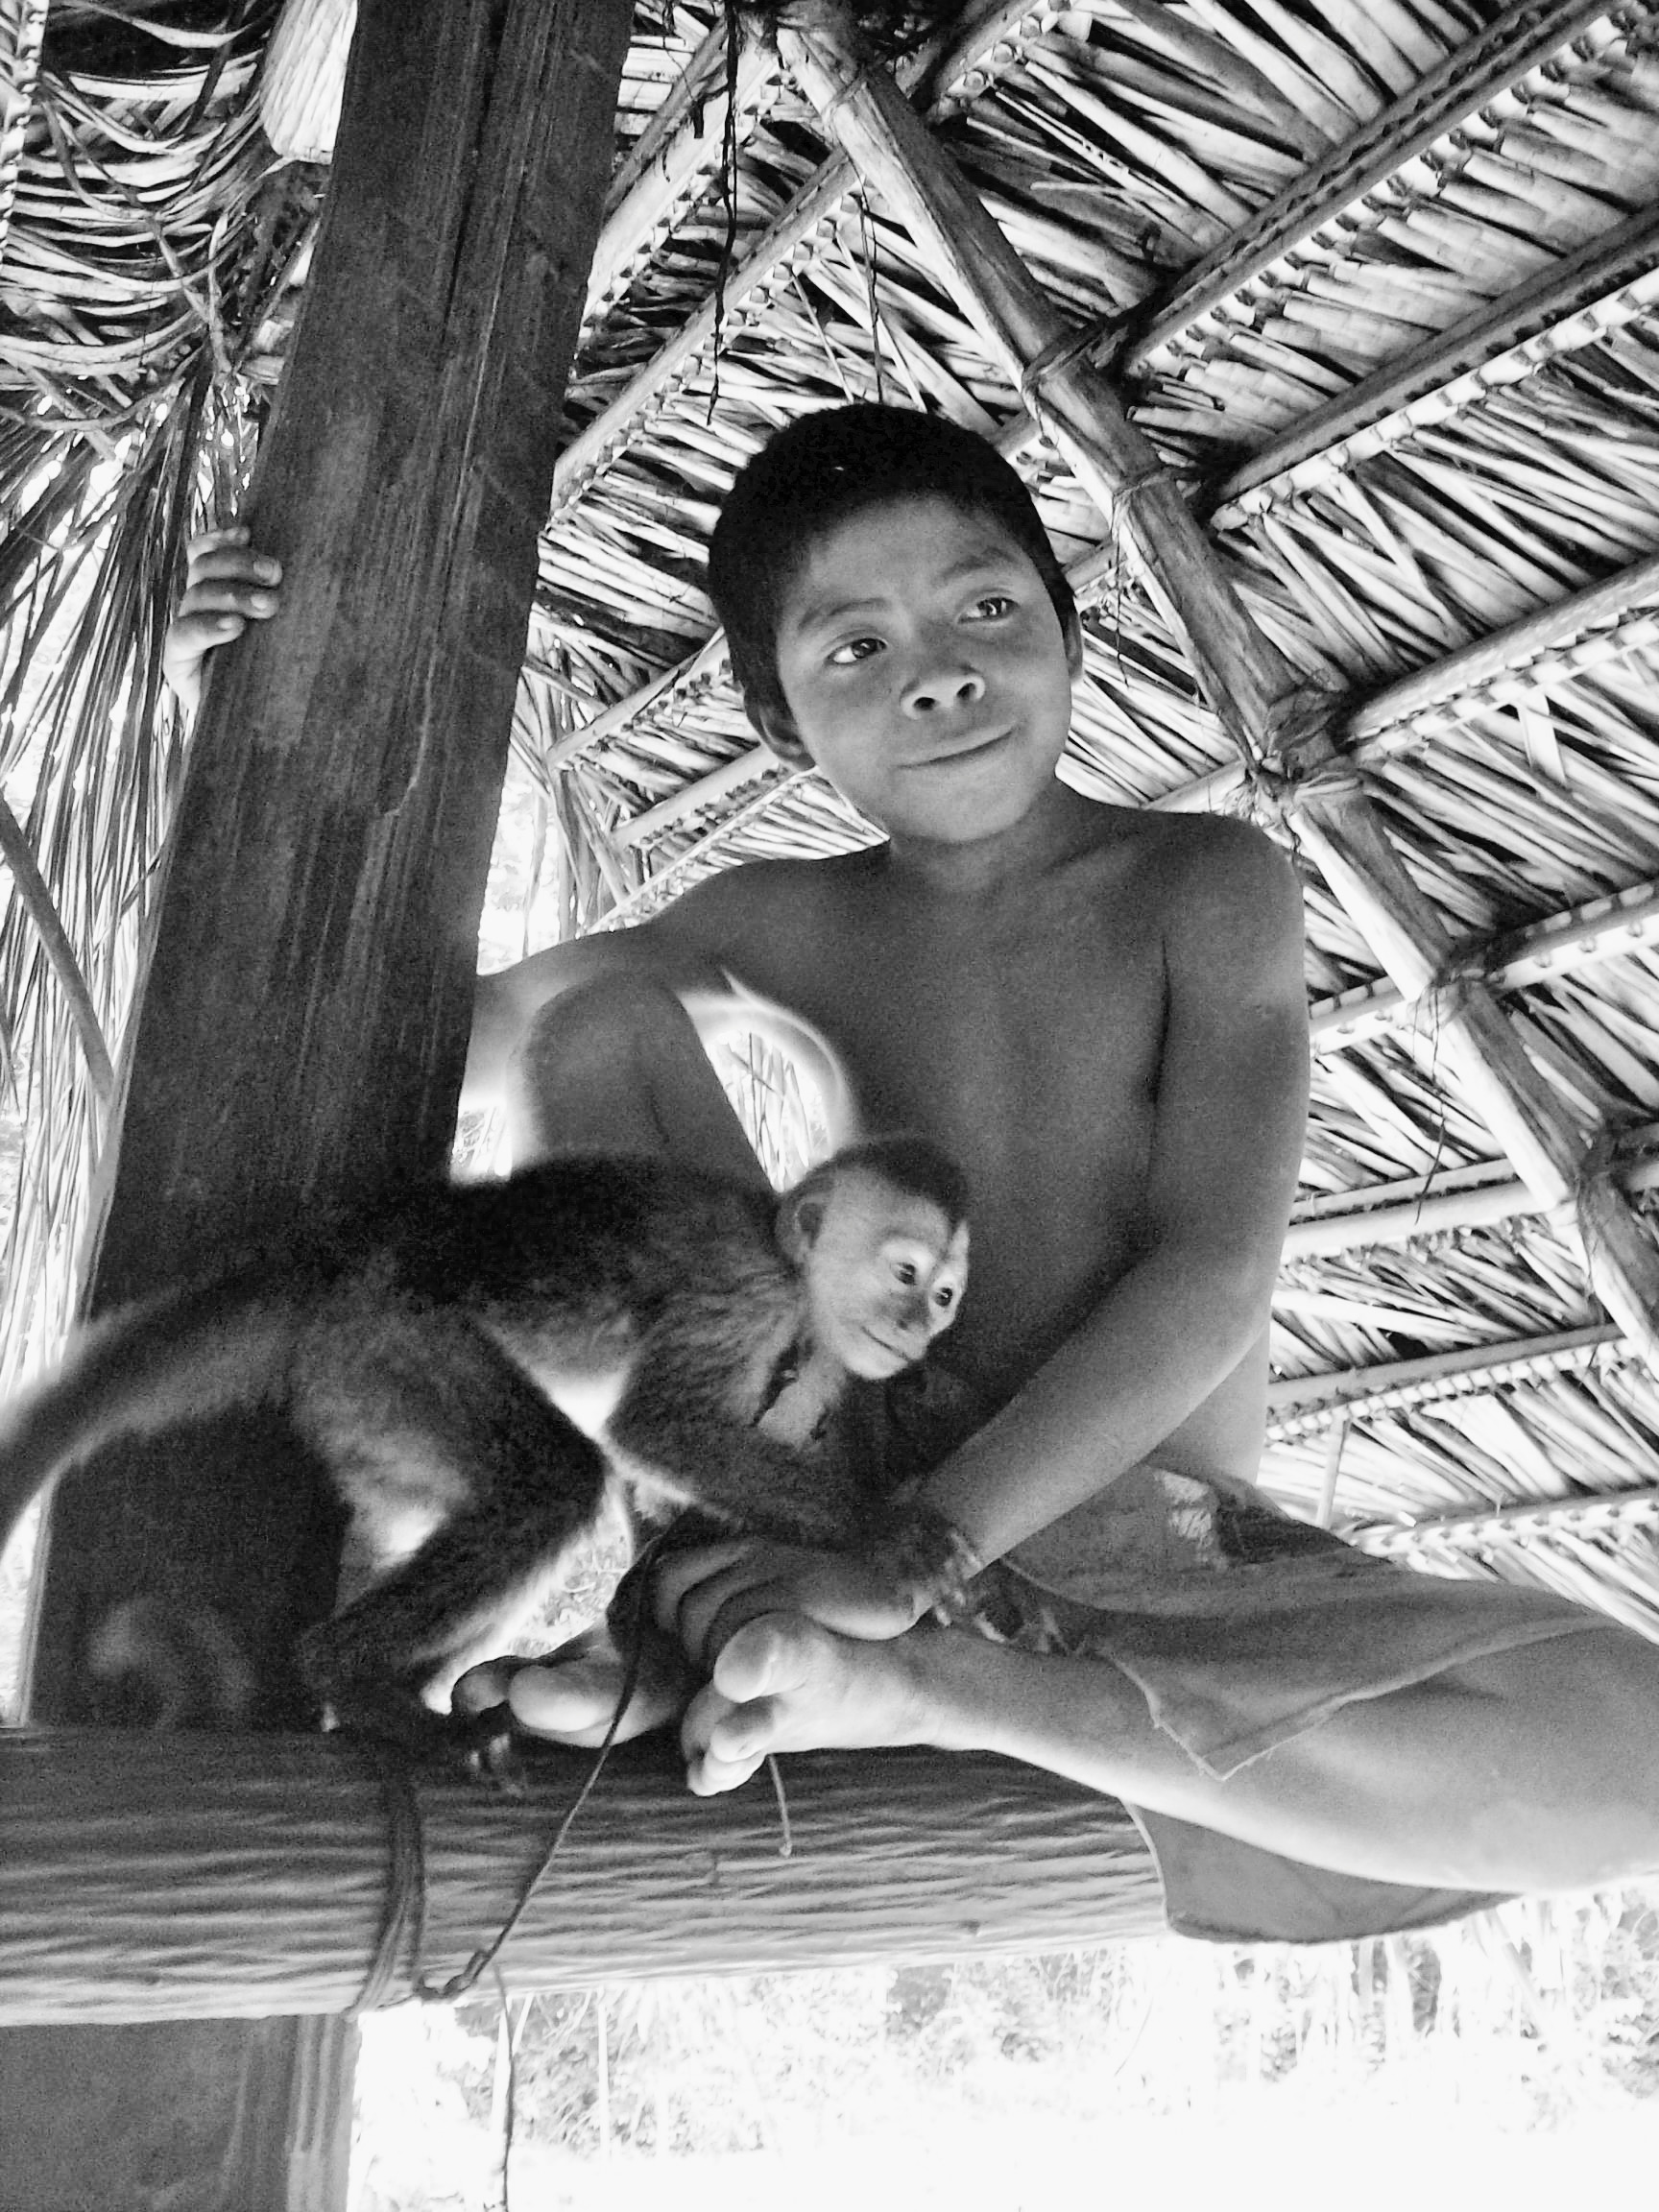
\includegraphics[width=97mm]{./imgs/100_4768}
%\caption{Takwari (ainda menino) sentado na viga do telhado de sua casa ao lado de um macaco cairara de criação (aldeia Juriti, 2007).}
%\end{figure}

\section{\textit{awa mỹna}, «a gente antiga»}

\noindent{}Quando sozinho no mundo, o herói cultural \textit{Maira}\footnote{Quando
  utilizado na forma independente, o nome \textit{Mai(r)} ganha o sufixo
  nominal ``\textit{a}'' e sua consoante final r é recuperada, e aparece
  como \textit{Maira}. Se utilizado com outro substantivo, prevalece a
  forma original \textit{Mai}, como em \textit{Mai} \textit{nima,} ``animal de
      criação de Maíra''. Farei aqui uso das duas formas, a depender da
  situação.} fez a primeira mulher na Terra a partir de um tronco de
árvore --- \textit{irakera,} ``aquilo que foi madeira'' ---, e a criação de toda a
humanidade é atribuída a esse fato. A sequência inicial desse
acontecimento pode ser interpretada como uma variante do tema da Noiva
de Madeira, ou a Noiva Esculpida em Madeira, discutido por Lévi-Strauss
em \textit{Do mel às cinzas}, ``encontrado em regiões muito distantes do
continente, desde o Alasca, entre os Tlingit {[}\ldots{}{]} até a Bolívia, onde é
objeto de um mito tacana {[}\ldots{}{]} Entre os próprios Warrau, encontramos
este mito sob a forma da história de um rapaz solteiro que esculpe a
mulher num tronco de buriti'' (1967 {[}2004{]}, p.\,201). Deste surgimento
da mulher esculpida na madeira pelo herói criador guajá e de sua
consequente gravidez, inicia-se um ciclo com o nascimento de dois
meninos gêmeos, um chamado \textit{Maira} e o outro, Gambá\footnote{Os
  nomes para o \textit{trickster} irmão de \textit{Maira}, Gambá
  (\textit{Didelphis marsupialis}, conhecido como ``mucura'' na Amazônia e
  sarigue em outras regiões do Brasil), podem ser \textit{Mukuxa'a}
  (``gambá'' com terminação final de nome próprio) ou mesmo \textit{Ajỹ},
  uma vez que o gambá é o principal avatar dos espectros \textit{Ajỹ}.
  Neste livro utilizo Gambá para me referir tanto ao irmão de
  \textit{Maira} quanto a mucura, ou sarigue, em geral.} (Mucura ou Sarigue),
cujas aventuras deixam marcas visíveis na Terra até os dias atuais.
Combinando mitologia e sociologia, esse capítulo se interessa por um
tema clássico da etnologia sul-americana --- e da antropologia --- definido
de maneira genérica como \textit{noção} \textit{de pessoa}. São discutidas
aqui as formas de \textit{subjetividade awa}, a partir da descrição
dos componentes que marcam a humanidade --- \textit{awatea}, ``gente de verdade'' ---, as concepções sobre o corpo e a vitalidade, além de uma
antropologia interessada nas alegrias, tristezas, sonhos, onomástica,
comensalidade, enfim, elementos que compõem a própria existência.

À guisa de introdução, apresento uma sequência de acontecimentos míticos
cuja unidade das narrativas compõe um tema mais amplo, referente à
origem da primeira humanidade, pensados como \textit{awa mỹna}, a ``gente
de antigamente''.

Embora os Guajá narrem poucos mitos, penso que os transcritos adiante
são uma boa apresentação sobre os habitantes do mundo. Não é intenção
desta obra produzir análise mítica exaustiva; destaco-os apenas por
serem ``histórias''\footnote{\textit{Mumu'ũ}, ``ensinar'', ``contar''; e
\textit{mumu'ũaena}, ``o que foi dito'', ``narrativa''.} que os Guajá
relataram, muitas vezes para se referir a alguma situação ou explicar
determinadas coisas do mundo. Esses mitos aparecem transcritos com
repetições de frases e ideias, porém tais repetições são relativas à
forma como são contados, com pausas, anáforas e outros recursos que
marcam as narrativas. Assim, minha intenção é manter certo ritmo oral,
tal como alguns mitos parecem exigir. Ouvi essas narrações na aldeia
Juriti, Tiracambu e Awá e agradeço aos homens Wiraho, Takya, Pirama'ã,
Ka'awi'ia; na aldeia Tiracambu, Kamairu; e na aldeia Awá,
Hajkaramykỹa, Irakatakoa e Tatuxa'a. Também agradeço a Panapinuhũ, a
única mulher que o fez. Alguns foram relatados em português, e outros,
em Guajá.

\subsection{A noiva de madeira}

\textit{Mairua}\footnote{Literalmente, ``o pai de \textit{Maira}:\textit{Mai}, de ``\textit{Maira}'', junto ao sufixo \textit{r-ua}, ``pai de''.}
não tinha esposa e passou muito tempo sozinho, até que um dia viu uma
árvore. A árvore tinha um tronco com formas que, ligeiramente, lembravam
um corpo humano. De seu tronco ramificavam galhos que, vagamente,
lembravam braços, e sua base se estendia pelo chão em raízes aéreas que
mais pareciam pernas. Após tanto procurar, o demiurgo escolheu essa
árvore para transformar em sua esposa. ``Eu não tenho esposa, vou fazer
deste pau a minha esposa'', disse \textit{Mairua}, que cortou um pedaço do
tronco e cantou, cantou, cantou; assim, fez aparecer as mãos, os braços,
seios, pés, pernas, cabeça, olhos, boca, nariz e vagina. E o tronco se
transformou em mulher. O herói também fez \textit{tapaja} --- a ``saia'' --- para
sua criação, e então ela se transformou em \textit{awa wahya}, ``mulher''.
Quando essa primeira mulher surgiu, perguntou a \textit{Mairua}: ``Eu vi o
que você fez. Por que você me fez assim?'' ``É assim mesmo'', respondeu o
demiurgo, ``eu não tinha esposa, e agora tenho''. Logo depois fizeram sexo
e ganharam filhos.\footnote{Os mitos a seguir se relacionam diretamente
  com o ciclo mítico dos gêmeos Tupinambá trabalhados por Lévi-Strauss
  em \textit{História de Lince} (ver Lévi-Strauss, 1993).}

\subsection{A fuga de \textit{Mairua}, o pai de \textit{Maira}}

Houve uma época em que os pequizeiros só davam flores, e a fruta do
pequi, \textit{myky'á}, não existia. Assim, \textit{Mairua} falou para sua
esposa:

--- Vá pegar pequis para comermos!

Ela lhe responde que não e diz: 

--- Dos pequizeiros só brotam florzinhas.

--- Então vá lá olhar!, disse \textit{Mairua}.

A ``mulher-pau'' de \textit{Mairua} não quis ir e disse: --- Não vou, lá só
tem florzinhas e frutinhos bem pequenos, eu sei. Do pequizeiro não
nascem grandes frutos.

\textit{Mairua} ficou bravo com sua esposa.

--- Eu vou embora para longe de você. Você não é uma boa esposa para mim ---
disse o demiurgo.

\textit{Mairua} pegou suas flechas e foi embora. A esposa dele estava
grávida de gêmeos; um deles, muito sabido, por isso falou de dentro da
barriga para sua mãe:

--- \textit{Amỹ},\footnote{Em português, ``mamãe''.} vamos sair e procurar por meu pai!

Os meninos se chamavam \textit{Maira}\footnote{Tal como na mitologia
  Tupinambá, a mitologia Guajá narra as aventuras de \textit{Mairua}, que
  logo sairá de cena cedendo lugar a seu filho \textit{Maira} e seu irmão
  \textit{Gambá}, como veremos. Enquanto os Guajá destacam dois demiurgos,
  pai e filho respectivamente, na mitologia Tupinambá encontramos seis
  gerações do demiurgo: (1) Monam, o primeiro humano; (2) Maira-Monam;
  (3) seu filho Sumé que teve dois filhos; (4) Maira-Pochy, um dos
  netos de Maira-Monam; (5) o filho de Maira-Pochy, apenas chamado
  Maira; (6) e Maira-Ata, sexto e último demiurgo (Lévi-Strauss,
  1993, p.\,51 e 57). De acordo com Lévi-Srauss: ``Ehrenreich, e Métraux em
      seguida, estima, provavelmente com razão, que as divindades que se
      sucedem e se substituem ao longo do relato constituem uma só; que são,
      como diz Métraux, desdobramentos umas das outras'' (Lévi-Strauss, 1993,
  p.\,56).} (tal como o pai) e \textit{Gambá},\footnote{Há uma versão desse
  mito que me foi narrada por meu amigo Hajkaramykỹa, que parece ser
  idêntica à de Thevet, trabalhada por Lévi-Strauss em \textit{História de
  Lince}. De acordo com o relato de Hajkaramykỹa, a esposa de Maíra
  engravidou de \textit{Mairua} (pai de \textit{Maira}) e \textit{Mukuxa'a}
  (gambá) que seria o pai de Gambá, irmão de Maira. A mulher então seria
  mãe de gêmeos, porém com genitores diferentes. Na versão de Thevet
  para o mito Tupinambá, a mulher engravida de duas crianças a partir de
  pais diferentes: um dos gêmeos é filho de ``Maira-Ata'', e o outro é
  fruto de um estupro cometido por ``Gambá'' (Lévi-Strauss, 1993, p.\,59).}
\textit{Mukuxa'á}. A mulher, carregando os dois filhos no ventre, andou,
andou, andou, até encontrar as pegadas de \textit{Mairua}. Daí continuou
andando até encontrar folhas muito bonitas, e o bebê \textit{Maira} diz
para sua mãe:

--- \textit{Amỹ}, pegue essas folhas para mim!

As folhas estavam repletas de marimbondos que picaram toda a mãe do
pequeno \textit{Maira}. Ela ficou muito machucada e brava por causa das
picadas que levou. Gritando, disse para o filho que carregava no ventre:

--- Por que você me pediu essas folhas? Eu estou toda machucada! Você quer
comer folhas? Por que você quer comer folhas? Agora, e por isso, eu vou
matar vocês dois.

A mulher começou a bater na própria barriga com muita força, ``pá, pá,
pá'', certa de matar os gêmeos. Surpreendentemente, apesar das diversas
pancadas, \textit{Maira} e \textit{Gambá} não morrem. Eles são muito fortes.
Depois das pancadas que a mãe desferiu na própria barriga, \textit{Maira}
cessa o diálogo com sua mãe.

Então, a mãe lhe pergunta:

--- Onde está o seu pai, que eu não o acho?

\textit{Maira}, de dentro da barriga, nada responde, pois está zangado com
sua mãe. A mulher continuou a caminhar pela floresta em busca de seu
marido, até que encontrou o rastro de alguém. Ela não sabia que se
tratava de pegadas de onças e imaginou ser o caminho aberto por seu
marido, \textit{Mairua}. E pensou:

--- Acho que meu marido está por aqui. Sim, ele foi por aqui mesmo.

E seguiu pela trilha.

\subsection{A aldeia das onças}

A esposa de \textit{Mairua} seguiu pela trilha até encontrar uma mulher,
jovem e bela. Era uma ``mulher-onça'', \textit{jawa wahya}, esposa de um
homem-onça, \textit{jawara}. Essa mulher estava cozinhando animais da
floresta como caititus e veados. Nessa época, as onças, que eram humanos
--- embora um pouco diferentes, pois também gostavam de carne crua ---,
dominavam o fogo. De dia eram gente e à noite viravam onça e saíam para
caçar. A mulher-onça enxergou a esposa de \textit{Mairua} e a chamou:

--- Venha para cá! --- disse a onça.

--- Estou procurando meu marido, você o viu? Ele me largou --- disse a
esposa de \textit{Mairua}.

--- Não eu não o vi. A minha casa é aqui e eu não vi ninguém passar. Eu
sou uma onça, o meu marido também é uma onça, nós não somos \textit{awa}.
Fique aqui conosco, você será a minha neta, \textit{hamijarua}. Eu vou
criar você como uma neta --- falou-lhe a mulher-onça.

A mulher de \textit{Mairua} aceitou a proposta. Assim a mulher-onça
retirou algumas palhas e prontamente construiu uma casa em forma de
tocaia, bem fechada, para que a mulher lá se instalasse sem que seu
marido-onça, um devorador de carne humana, a visse.

--- A partir de agora você vai dormir nesta casa, disse a mulher-onça. O
seu marido, \textit{Mairua}, foi para muito longe, e você não vai mais
encontrá-lo.

No final da tarde, o marido da onça voltou de uma caçada. Por isso sua
esposa-onça falou baixinho, sussurrando:

--- O meu marido está chegando, eu consigo ouvi-lo, \textit{shhhhhh}!

O marido-onça traz consigo alguns pedaços de carne e cabeças de caititu
e veado. Os outros pedaços ele comeu crus, ainda na floresta. No caminho
para sua casa ele encontrou as pegadas da esposa de \textit{Mairua} e, ao
chegar em casa, jogou a carne no chão perguntando para a esposa:

--- Você viu algum humano, \textit{awa}, por aqui? Eu encontrei pegadas aqui
perto.

--- Não, eu não vi nenhum humano, estou sozinha em casa --- respondeu a
mulher-onça.

--- Mas eu encontrei as pegadas de um humano no caminho, e as pegadas
vinham nesta direção --- insistiu o homem.

--- Não há ninguém aqui. Eu vi uma mulher, mas ela foi-se embora por ali --- disse a mulher-onça.

--- Não, ela não foi embora! --- disse o marido-onça, convencido de que a
humana ainda estava em sua aldeia.

De repente um vento soprou, e a onça consegui sentir o cheiro da mulher
que vinha de dentro da sua casa-tocaia, pois de todos os animais a onça
é o que melhor sente o cheiro dos humanos. Quando o marido-onça viu a
tocaia, concluiu:

--- Ah, aqui está! Essa tocaia não estava aqui antes, alguém a construiu.

O homem-onça invadiu o abrigo, mas sua esposa gritou em cima:

--- Não coma ela! Ela é nossa \textit{harapihianã} (parente por afinidade).
Você já comeu muito caititu, veado e outros bichos no mato, para que
comer essa humana?

Mas a onça, \textit{crau}, comeu-lhe a cabeça. Depois comeu tudo: os braços, a
pele, comeu tudo. Tirou a tripa, tirou tudo e comeu; não tem mais a mãe
de \textit{Maira}. Só sobraram-lhe os filhos na barriga, que a esposa-onça
pediu para comer:

--- Você está comendo toda essa mulher, então me dê os filhos dela para
que eu também os devore. Deixe eu comer também!

--- Está bem --- disse o marido.

\subsection{O nascimento dos gêmeos}

Com o auxílio de uma faca, o homem-onça abriu a barriga da mulher morta,
tirou as duas crianças, e deu à sua esposa para que comesse. Ela,
bastante chateada, passou a maldizer o marido por ter feito tamanha
maldade àquela mulher. Mesmo assim, para agradar o marido, a mulher-onça
colocou os dois bebês perto de pedaços de animais que seriam limpos por
ela antes de assados.\footnote{Em outra versão, a mulher-onça tem piedade
  das crianças e quem decide cozinhar os gêmeos é outra mulher (também
  onça) da mesma aldeia.} Após limpar os animais caçados, ela pegou os
dois bebês \textit{Maira} e \textit{Gambá} e pensou:

--- Vou cozinhá-los mesmo!

Pôs água dentro de uma panela e em seguida colocou os gêmeos, mas eles
pularam para fora da panela.

--- Que diabos é isso? --- pensou a mulher.

Colocou-os novamente dentro da panela, e novamente eles pularam para
fora. Assim aconteceu seguidas vezes. Eles eram muito espertos. Ela os
botava para dentro da panela e eles pulavam para fora ao sentir a água
quente. A mulher-onça então disse:

--- \textit{Ariku ta hanima neme}, ``vou criá-los como\footnote{Pode ser entendido como uma expressão próxima a ``ficar com eles
como'', ou ``transformá-los em''.} meus seres de criação''. Eles são meus
\textit{harapihianã}, ``afins'', eu vou criá-los como se fossem meus netos.
Vou pô-los no rio.

Por isso, aproveitou que seu marido fora caçar na floresta e colocou os
dois meninos, que ainda estavam na placenta, dentro do rio para acabar
de gestarem. O marido-onça, embora possuísse arco e flecha, caçava
somente com suas garras e dentes. Passado algum tempo, os gêmeos
cresceram, cresceram e cresceram, a placenta rasgou e os dois meninos
nasceram. Assim que saíram da placenta procuraram pela mãe:

--- Cadê a nossa mãe? Onde está nossa mãe? --- procuravam os gêmeos.

A mulher onça respondeu:

--- A mãe de vocês foi embora. Agora eu sou a mãe de vocês. Podem
acreditar em mim, eu sou a mãe mesmo. Eu mesmo!

--- E cadê o nosso pai? --- perguntaram

--- O pai de vocês foi caçar. Foi caçar caititu, veados, queixadas ---
referindo-se ao marido-onça. Comam essa carne aqui --- ofereceu a mulher
aos meninos.

A mulher-onça deu para eles comerem um pouco de uma carne bem macia,
pois eles já tinham dentes, e \textit{Gambá} comeu um pouco da carne.
Passado um tempo, o homem-onça voltou de sua caçada trazendo caititus,
veados e queixadas. Quando viu os meninos, perguntou:

--- Quem são essas duas crianças?

--- São nossos netos --- disse a mulher-onça. --- Eles apareceram aqui,
deixe eles aqui, não os coma! Eu vou criá-los --- disse ela ao
marido.

--- Pode deixar, eu não vou comê-los --- respondeu a onça.

Então eles cresceram, cresceram, cresceram. Fizeram suas próprias
flechinhas. E nessa época mataram muitos passarinhos. E chegaram em casa
falando:

--- Vovozinha, nós matamos passarinhos!

--- Quantos passarinhos vocês mataram?, perguntou a avó.

--- Estão aqui, olha quantos, vovozinha. Matamos dezenas de passarinhos,
vovozinha. Matamos tantos que parecem capelães, de tanto que matamos.
Caçamos chora-chuva preto, juriti-gemedeira, urus, nhambus, pariris,
rolinhas, pombos, tá tudo aqui, vovozinha!

A onça-avó ficou feliz com a caçada de seus netinhos e se deliciou com
tantos pássaros. Ela cozinhou tudo em panelas, do jeito que a gente-onça
gostava de comer. \textit{Maira} estava se tornando um grande caçador já em sua
primeira infância. Eles continuaram crescendo, crescendo, crescendo\ldots{}
Passado algum tempo, os gêmeos tornaram-se adultos.

\begin{center}\adforn{68}\end{center}

A partir de agora, \textit{Maira} e \textit{Ajỹ} inauguram um ciclo de
acontecimentos que dão origem a muitas das coisas do mundo, tal como os
Guajá conhecem hoje; além de explicar, em parte, o aparecimento dos
humanos. Vejamos o que nos interessa, por hora.

\subsection{O surgimento dos inajás e das ariranhas}

\textit{Maira} pensou e disse para seu irmão, \textit{Gambá}:

--- Vamos fazer o inajá aqui.

--- Para quê? --- perguntou \textit{Gambá}.

--- Para comer --- respondeu \textit{Maira}.

\textit{Maira} e \textit{Gambá}, juntos, fizeram brotar cachos de inajá
instantaneamente. Os inajás feitos por \textit{Maira} eram os amarelos
dourados --- \textit{pirỹma'a}, ``avermelhado'' ---, enquanto \textit{Gambá} fez
inajás brancos, que são muito ruins. Havia muitos inajás, e eles
resolveram levar para sua mãe-onça. Fizeram dois \textit{marakũa} --- sacolas, mochilas confeccionadas com folhas frescas. \textit{Maira} levou
um \textit{marakũa}, e \textit{Gambá} levou o outro. A mulher-onça estava em
casa, porém não conhecia inajás. Quando ela viu os gêmeos voltando,
falou:

--- Venham logo! Onde vocês estavam? O meu marido-onça vai comê-los se
ficarem sozinhos pela floresta.

Quando chegaram em casa, falaram:

--- Mãe, trouxemos inajás.

--- Vocês sabem produzir o inajá?

--- Sim, nós sabemos e fizemos, aqui está! --- disse \textit{Maira}.

A mãe-onça colocou os inajás no fogo e os cozinhou. Depois de cozidos,
comeu e disse:

--- Nossa, mas esses inajás são bem grandes e muito gostosos.\footnote{Vale
  lembrar que, no tempo dos mitos, os frutos eram maiores do que são nos
  tempos atuais.} Onde vocês conseguiram? Eu quero ver esse inajazeiro,
vocês me levam até lá?

--- Vamos lá, é por aqui! --- disseram os gêmeos convidando a mãe para
coletar mais inajás.

A mãe-onça foi seguindo seus netos, ou ``filhos'', até chegar ao
inajazeiro. Era uma árvore magnífica que produzia inajás muito grandes,
maiores do que os encontrados atualmente. Ela coletou muito desses
frutos e voltou para casa com seus filhos para cozinhá-los. Chegando à
aldeia, cozinhou-os e enquanto comia jogava suas cascas perto de casa. O
\textit{Jaku Jara}, um jacu humano, que era muito sabido, então falou
para \textit{Maira}:

--- Meu \textit{harapihianã}, ``afim'', você mora junto com a onça, mas você
não deve morar junto dela. Ela não é sua mãe como você pensa. Ela comeu
a sua mãe de verdade. Ela te pegou para criar e se tornou sua avó, mas
ela nunca foi sua mãe.

--- É mesmo? --- disse \textit{Maira}, atônito. --- Então espere, pois eu vou
fazê-las, as onças, virarem ariranhas, \textit{jawatara}.

Nisso, o homem-onça volta de sua caçada habitual trazendo porcos,
caititus, veados mateiros e veados fobocas. A onça não caçava antas,
pois este animal tem o couro muito duro. Quando a onça viu os inajás,
perguntou:

--- O que é isso? Quem fez esses frutos?

--- Os nossos netos sabem fazer inajá; foram eles que fizeram --- disse a
esposa-onça. --- Eles fizeram muitos inajazeiros por aí, muitos, muitos.

--- Então vamos comer! --- disse o marido-onça.

--- Vá lá, eu vou ficar aqui --- respondeu-lhe a esposa.

O homem-onça comeu muitos inajás, junto com as outras onças; e pegaram
outros para levar para casa. Na volta, enquanto a esposa-onça estava
limpando os animais em casa para cozinhar, as onças que voltavam
passaram por uma ponte no caminho. Enquanto passavam pela ponte,
\textit{Maira} conseguiu derrubá-la dentro d'água, fazendo com que as
onças caíssem. Ao cair, elas foram devoradas por piranhas, \textit{ipinẽa}, muito grandes, e seus ossos viraram ariranhas. As
ariranhas, que eram os ossos das onças, foram embora nas águas. Logo
depois, outro grupo de onças voltava pela mesma ponte, e \textit{Maira}
conseguiu derrubar a ponte novamente, fazendo com que esse grupo de
onças também caísse n'água. As piranhas também as devoraram, e seus
ossos também viraram ariranhas.

Em seguida, mais onças vieram pelo caminho, e \textit{Maira}, junto com
seu irmão, \textit{Gambá,} conseguiu transformar as onças em veados,
fazendo com que os veados saíssem correndo pela mata. \textit{Maira} fez
isso várias vezes. Certa hora, o demiurgo sentiu vontade de defecar e
pediu para que seu irmão continuasse transformando as onças em
veados-mateiros, \textit{arapaha}, e veados-fobocas, \textit{arapaha'í},
mas o alertou:

--- Eu vou cagar. Não faça nada de errado e continue o que estamos
fazendo!

Enquanto \textit{Maira} fazia suas necessidades, ficou observando o irmão.
Uma onça veio pela ponte e \textit{Gambá}, meio atrapalhado, não conseguiu
transformá-la em veado, deixando-a na forma de onça. \textit{Maira} voltou
rapidamente e esbravejou com \textit{Gambá}:

--- Você não está fazendo direito. Não faça desse jeito ruim, você deve
transformá-las em veados.

---Tá bom --- respondeu \textit{Gambá}.

\textit{Maira} voltou para suas necessidades, e novamente \textit{Gambá}
deixou as onças passarem sem que fossem transformadas em veados. E
\textit{Maira} brigou novamente com seu irmão:

--- Você não fez direito! Deixou as onças irem embora, agora elas
vão nos comer para sempre. Vamos voltar para casa!

Quando retornaram para casa, a mãe-onça lhes perguntou:

--- Onde está meu marido?

--- Não sei. Parece que ele está comendo inajás. Depois virá para casa ---
responderam os dois de maneira dissimulada.

\subsection{O surgimento do gavião}

A mãe-onça de \textit{Maira} pede que seu filho cate piolhos, \textit{ikya},
de sua cabeça. Enquanto ele o fazia, a mãe-onça adormeceu.
Aproveitando-se da situação e para vingar sua verdadeira mãe que fora
morta pelas onças, \textit{Maira} e \textit{Gambá} cortaram-lhe a cabeça.
Depois pegaram a cabeça da onça, fizeram-lhe nascer penas e ela se
transformou em gavião. A mãe-onça ficou deitada sem cabeça em sua rede,
e \textit{Maira} foi embora procurar seu pai, \textit{Mairua}.

\subsection{Coda}

A partir desse episódio, quando \textit{Maira} e \textit{Gambá} matam a
mãe-onça e vão embora pelo mundo, um conjunto de mitos consolida os
gêmeos como precursores da humanidade, de quem todos os Guajá
descenderiam. É \textit{Maira} que traz a especiação dos seres e, após a
Terra, \textit{wya}, estar pronta, com sua paisagem atual concretizada,
outros humanos selvagens, \textit{mihua}, atentam contra a vida de
\textit{Maira} envenenando-o. E ele, mesmo sobrevivendo, parte para o céu
junto com seu irmão gêmeo, e lá vivem até hoje.

\section{\textit{awatea}, «gente de verdade»}

Utilizado por diversos grupos Tupi-Guarani da Amazônia --- como os
Parakanã (Fausto, 2001), Asuriní do Xingu (Müller, 1993), Aikewara
(Calheiros, 2014, p.\,7), Ka'apor (Balée, 1994) ---, o termo \textit{awa}
aparece aqui como a forma pela qual esse povo se identifica, encontrando
em ``humano'' ou ``gente'' as melhores traduções, em oposição a outros
termos como \textit{kamara}, outros indígenas, \textit{karaia}, não
indígena, e \textit{mihua}, gente-selvagem, como veremos. \textit{Awá} são
homens e mulheres. \textit{Wanihã}, homens, e \textit{wahya}, mulheres, de um
mesmo universo. Os Guajá se pensam como \textit{awatea},\footnote{\textit{Awa},``humano'' junto ao sufixo
\textit{te}, ``real, verdadeiro''.} idêntico inclusive ao termo na língua
parakanã (Fausto, 2001, p.\,39) que pode ser traduzido como ``gente de verdade''\footnote{Ver também Cormier, 2003, p.\,89.} Muito mais do que ``a
humanidade como espécie natural'', a categoria \textit{awa} denota uma
``condição social da pessoa'' (Viveiros de Castro, 2002, p.\,371), que
neste caso, bem como em tantos outros povos ameríndios, consiste em uma
composição própria do corpo, além de um gradiente social formado por uma
série de oposições que se inicia nos humanos próximos e se estende às
esferas de parentes mais distantes, até chegar aos grupos inimigos e
outros seres perigosos como os seres-espectro \textit{Ajỹ}.

Fisiologicamente, os Guajá definem a pessoa humana como constituída por
três elementos característicos: \textit{ipirera}, \textit{hajtekera} e
\textit{ha'aera}, respectivamente. Ou, como traduzem para o português:
``meu couro'', \textit{hapirera}, ``carne'', \textit{hajtekera}, e ``raiva'', \textit{ha'aera}. Em linhas gerais, e como gostam de ilustrar, quando
uma pessoa morre, seu ``couro'' permanece na Terra até apodrecer, e sua
``carne'' vai para o \textit{iwa} --- um conjunto de patamares celestes;
enquanto a ``raiva'' segue para a floresta, \textit{ka'a}, para o
mato, de preferência para os locais recônditos, e se transforma em \textit{ajỹ}\footnote{Espectros necrófagos que vivem na floresta, atacam os humanos com
doenças e têm os gambás como animais de criação.} Noções centrais para o
entendimento da sociocosmologia \textit{awa}, \textit{ipirera},
\textit{hajtekera} e \textit{ha'aera} são os princípios que promovem a vida
e possibilitam a separação da pessoa após a morte. Poderíamos traduzir
grosseiramente \textit{ipirera} por ``corpo-pele''; \textit{hajtekera} por
``vitalidade'', cujo correspondente ocidental, apenas como paralelo, seria
``alma''; e o \textit{ha'aera}, por ``raiva'' ou ``alma penada''. Tentarei
esboçar aqui como tais ideias tornam complexo o dualismo corpo e alma ou
material e espiritual, e não são representações do que seria a pessoa
humana em seus aspectos material e imaterial. Pelo contrário, esses três
elementos embaralham de alguma forma noções fisiológicas centrais --- como
anatomia e sintomatologia ---, pois aqui, elementos do corpo físico
transcendem a ideia de ``físico''. Em outras palavras e de maneira bem
direta, o corpo aqui é muito mais --- ou menos --- do que o suporte do
\textit{hajtekera} --- alguns elementos do corpo também são o próprio
\textit{hajtekera}, e isso nos fornece uma terminologia apropriada para o
entendimento das relações humanas.

\section{viver, morrer}

Antes do contato, quando a morte de alguém ocorria o mais comum era
abandonar a área onde viviam, deixando para trás o cadáver, \textit{ipirera}. Durante as caminhadas, qualquer espaço servia para
deixar um corpo: no meio do mato longe do caminho, \textit{pea}, em um
buraco dentre tantos feitos pela erosão ou animais na floresta e mesmo
dentro de uma árvore oca e caída, apodrecida na paisagem. O morto era
deixado para trás. Se a morte ocorresse dentro de casa, deixavam o
cadáver em sua rede e derrubavam a casa --- \textit{tapãja}, ``tapiri'' --- sobre
o morto, partindo para longe, e montavam uma nova aldeia que, como
vimos, muitas vezes consistia em uma única casa. Se a morte ocorresse
durante uma caminhada, simplesmente abandonavam o corpo e permaneciam
longe da área de morte por um longo período de tempo. A única exceção
são os recém-nascidos, os natimortos. Quando ocorre de um bebê morrer no
parto, e só nesses casos, ele é enterrado dentro de casa, pois as
pessoas ainda não se ``acostumaram'', \textit{amimakwa}, à criança. As
pessoas evitam locais onde ocorreram mortes recentes ou com sepulturas,
uma vez que os fantasmas \textit{ajỹ} costumam frequentar tais locais.
Desde o contato com a Funai, foram criadas próximas às aldeias áreas
para ``enterro'', é prática dos funcionários do posto enterrar as pessoas
mortas. Quem faz esse trabalho desagradável são os \textit{karaia} da Funai, 
já que os Guajá pouco manuseiam ou enterram seus mortos em
sepulturas. Desde a fixação em aldeias a partir do contato, muitas
pessoas faleceram de gripe e malária, e os Guajá passaram a conviver com
o ``mal-estar'' de viver próximos aos mortos. No ``tempo do mato''
--- \textit{imỹna}, ``antigamente'' ---, os velhos e moribundos eram abandonados,
pois quando a morte se aproximava não era seguro permanecer ao lado de
alguém prestes a sucumbir. Até os dias de hoje, as pessoas muito velhas
podem, ou não, receber um tratamento de abandono. Uma das situações que
mais chamavam atenção dos funcionários da frente de atração na época do
contato --- disse-me certa vez um funcionário aposentado que conheci --- era o
fato de muitas pessoas aparecerem para o contato afirmando terem deixado
para trás seus parentes mais velhos --- pais e avós ---, uma vez que esses se
recusavam a se encontrar com os \textit{karaia}. Os Guajá que passaram a
viver nas imediações do \textsc{pin}, por outro lado, nunca mais voltariam a
viver com esses velhos que foram deixados para trás para morrer.
Kamairua, um amigo da aldeia Tiracambu, se lembra do pai --- nos anos de
fuga para evitar o contato --- que pedia para ficar para trás e exortava os
parentes a fugirem para longe, dizendo que estava velho, sem forças para
fugir e que iria morrer sozinho.

Como exemplo, \textit{Amirixa'a} é mãe de Muturuhũ, um homem importante na
aldeia Juriti. Ela é a mulher mais velha dessa aldeia, com idade
estimada em 89 anos, em 2008. Dentre todos, ela é a única que vive em
um tapiri, na periferia da aldeia; e dentre as mulheres, só ela veste
uma saia trançada com fibra de tucum, como era comum entre os
Guajá.\footnote{Hoje as mulheres preferem saias tecidas com linha e panos
  que ganham ou retiram de outras peças de roupas.} Amirixa'a produz a
própria comida: carrega pesadas cargas com macaxeira ou banana que
retira da roça; caça tatus e jabotis por conta própria. Ninguém a ajuda,
em nada. Se ela não procurar comida, não comerá. Devido a sua idade
avançada, sua dieta é livre de restrições, come qualquer coisa,
inclusive alimentos que causariam mal a outras mulheres: desde vísceras
variadas e fetos de inúmeros animais a carne de veados mateiros, \textit{arapaha}, e foboca, \textit{arapaha'i}. Há também uma dieta de
``antigamente'', \textit{imỹna}, composta por animais considerados
``repugnantes'', \textit{manyhỹ}, aos olhos dos jovens, mas que os velhos
podem e até gostam de comer, como uma rã chamada \textit{iwea}, feita
assada na brasa, e diversas espécies de ratos, \textit{awijỹa}, que depois
de limpos são assados em espetinhos. Antes do contato comiam isso tudo,
algo como uma ``dieta do mato'' --- \textit{ka'a nimi'ũa}, ``comida da
floresta'' ---, porém hoje em dia é comida de gente velha, pois essas
pessoas não passam mal com alimento quase nenhum.

Embora Amirixa'a receba esporadicamente pedaços de carne do grupo do seu
filho, ela possui seu próprio fogo e come separadamente das outras
pessoas. Pira'ima'ã, um de seus netos, explicou-me que Amirixa'a está
velha, \textit{tamỹ}, e não adianta o quanto de comida que deem a ela,
pois não vai se fortalecer. Não consegue se relacionar, pois se ela está
\textit{velha} está \textit{surda}, e se está \textit{surda} vai
\textit{morrer}. A surdez é o sinal mais evidente da presença, ou chegada,
da morte. E se tornar velho e surdo --- necessariamente nesta ordem --- é o
destino a que todos os Guajá estão sujeitos. \textit{Japijakoa myty}, ``ouvido entupido'', é uma das imagens mais utilizadas para se referirem
à velhice. Uma pessoa muito velha é uma pessoa surda; e uma pessoa surda
é um quase-morto.

Os velhos não conversam nem se relacionam porque não ouvem, a velhice
extrema como a de Amirixa'a é uma situação de não relação, porque ela
está muito velha para se casar novamente, conversar, cantar, ou qualquer
outra coisa. O fato de que, por consequência da velhice, as pessoas
dispensem menos cuidados a Amirixa'a não representa um descuido
deliberado, mas a aceitação de que o período de vida dela chegou ao fim
e que seu ``princípio vital'', \textit{hajtekera}, responsável justamente
pela sua ``vitalidade'' --- uma outra tradução para \textit{hajtekera} ---, não
mais lhe habita. A surdez, ela mesma, é associada à ausência do
\textit{haitekera}. Como Wiraho pontuou-me certa vez: ``nós estamos tão
acostumados com Amirixa'a, de vê-la todo dia, que quando ela morrer
vamos pensar --- Ah, ela não está mais conosco!, e vamos ficar muito
tristes''.\footnote{A ideia de abandono, e até mesmo aniquilamento dos
  idosos, é comum a diversos povos ameríndios. Descola apresenta a
  situação de uma velha que estava morrendo de doença em uma das casas
  que vivia e as pessoas tristemente diziam a ela: ``você está morta
      vovozinha, está morta'', enquanto ela ainda falava e pedia o que comer.
  E, diferente de outras doenças, as pessoas não procuravam intervir com
  medicamentos e outros tipos de ajuda. A mulher velha já era um cadáver
  (Descola, 2006, pp.\,407 e 409).} Nas noites de cantoria, quando seu filho
adentrava a \textit{takaja} para ir ao \textit{iwa}, a velha cantava
baixinho, de dentro de sua pequenina casa, para auxiliar o filho durante
sua viagem celeste. Em tais momentos todos paravam para ouvi-la,
alertando uns aos outros: ``\textit{Kwy!},\footnote{O ``\textit{kwy}'' é uma
  interjeição utilizada para exprimir surpresa, que pode ser comparado a
  ``Nossa Senhora!'', como falado em boa parte do Brasil.}
\textit{Amirixa'a jã}, ``Olhem, Amirixa'á está cantando!''; a mulher
parecia querer lembrar a todos que, mesmo solitária, ainda estava viva.

A convivência de pessoas em velhice extrema com outras em idades menos
avançadas é um ``fenômeno'' que passou a ocorrer com mais frequência após
o contato com a Funai. Desde a radical mudança na aparência e
funcionamento das aldeias, os velhos definham nas aldeias até morrer; e
quando morrem, os funcionários dos \textsc{pin} se encarregam de enterrá-los em
local próximo e reservado como cemitério. Nesse meio tempo, os Guajá ---
praticamente todos eles --- abandonam a aldeia por muitos dias e se
refugiam na floresta; pois, tal como sabemos a partir de outros povos
Tupi, os Guajá também têm pavor de cadáveres. Mais adiante veremos
melhor esse ponto. O luto, portanto, é um processo de esquecimento, \textit{imahare}, dos nomes, eventos e lugares relacionados à pessoa
morta que, aos poucos, é apagada da memória. Juriximatỹa certa vez me
contou ter ficado muito triste com a morte de seu cunhado To'oa; por
isso foi para a floresta logo que soube do fato e lá permaneceu durante
muitos dias, a fim de esquecer o falecido.

Da mesma maneira, por parte do morto, a morte é, da mesma forma,
``esquecer'' que foi vivo. Essa teoria é muito atuante entre os Guajá, que
dizem que ao chegarem no céu, após morrerem, se lembram pouco da vida na
Terra; e, à medida que se aproximam dos \textit{karawara}, vão perdendo a
memória, até o completo esquecimento de que foram vivos. Esse argumento,
a despeito de sua elegante simplicidade, é talvez o argumento mais
importante sobre o que seja ``morrer'', \textit{manũ}, para os Guajá. Não é
possível explicar a subida definitiva do \textit{hajtekera} para o
\textit{iwa} --- em outras palavras, \textit{morrer} --- sem mencionar o
esquecimento natural da vida terrena que o \textit{hajtekera}
experimentará no céu, \textit{iwa}. Por isso, discordo da interpretação
de Cormier --- baseada em outros autores (Geertz, por exemplo) --- ao
sustentar que a falta de compreensão genealógica dos Guajá pode ser
considerada ``amnésia genealógica'' (Cormier, 2003, pp.\,74--76). Os Guajá
simplesmente não querem falar dos mortos, e o ``esquecimento'' --- \textit{imahare}, ``esquecer'' ou ``não saber'' --- é um aspecto constituinte
do processo de luto e da morte. Eles esquecem o nome de pessoas das
gerações acima não porque sejam incapazes de lembrar, mas, ao contrário,
porque lutam para esquecer. Esse é um ``problema'' dos Guajá e de boa
parte da Amazônia indígena.\footnote{Ver Taylor, 1993.}

Quando do falecimento de uma pessoa --- \textit{manũ}, ``morrer'' ---, diz-se
\textit{hajtekera} \textit{oho iwape}  --- ``\textit{hajtekera} foi para o
\textit{iwa}''. E, depois de falecida, diz-se \textit{hajtekera} \textit{ikwẽ
iwape} --- ``a pessoa, ou \textit{hajtekera}, permanece no \textit{iwa}''. A
mim, ao falarem sobre a morte, era comum mencionarem em português que
determinada pessoa ``morreu'' ou ``subiu'', tal como se fossem sinônimos
para as situações de morte.\footnote{É bom lembrar que, assim como no
  português, os verbos ``subir'' e ``morrer'' são diferentes na língua
  guajá. \textit{Ipii} seria o equivalente a ``subir'' em português,
  utilizado, por exemplo, ao se referir a alguém que tenha subido em uma
  árvore: \textit{ipi ira rehe} --- ``ele subiu na árvore''. Além desses,
  pode-se dizer que algum indivíduo morreu utilizando-se a expressão
  \textit{oho iwape}, nesse caso, ``foi para o céu''.} Ao traduzir para o
português a ``morte'' por ``subida'', demonstram que o essencial da ideia de
morte, \textit{manũ}, é o deslocamento espacial da substância
\textit{hajtekera} --- que traduzo por ``princípio vital'' --- da Terra para o
céu. Porém, em diversas situações em que o \textit{hajtekera} abandona o
corpo, não obrigatoriamente implica morte. Nos dias de verão, quando
preparam a \textit{takaja} e homens de diferentes idades cantam com os
\textit{karawara} e com os mortos,\footnote{Discutiremos no último capítulo.}
encontramos um desses casos. Também, se uma pessoa se expõe a perigos e
privações, a reação natural é perder o seu \textit{hajtekera}. Vejamos
três situações em que pessoas perderam esse componente vital.

\paragraph{Perdido na floresta}

Durante uma caçada solitária, Wiraho se viu perdido na mata, \textit{pea
imĩ}, ``a trilha sumiu''. Longe de casa e sem saber como voltar, ele
ficou \textit{kije}, ``desesperado'' ou ``amedrontado'', algo que, por si só, já
é motivo para a fuga do \textit{hajtekera}, \textit{hajtekera oho}
\textit{iwape}. Ele conta que subiu ao \textit{iwa} sem qualquer mediação ---
do abrigo ritual da \textit{takaja}, sonho ou morte; de lá pôde ver o
caminho que havia perdido e quando desceu do \textit{iwa} já estava
próximo à sua casa.

\paragraph{O grande caçador}

Assim como Wiraho e tantos outros, Majhuxa'a, da aldeia Awá, que
é um grande caçador --- e como todo grande caçador, repleto de boas
histórias ---, também se perdeu na floresta. Muitos anos atrás, ``Majhu'', como é chamado carinhosamente, teve um encontro infeliz com a gente, \textit{awa}, que vive no mato, os chamados \textit{awa mihua}, os
``isolados'', e foi raptado por eles. Os \textit{mihua} são uma ``gente
braba'', \textit{awa imahy}, sabem os Guajá, e quiseram matá-lo a
flechadas.\footnote{Ainda nesse capítulo voltarei ao tema dos chamados
  ``isolados''. Os Guajá narram muitas histórias de encontros esporádicos
  na floresta com as pessoas, \textit{awa}, que vivem em isolamento
  voluntário.} Majhuxa'a, um sujeito calmo e calado, não me deu muitos
detalhes sobre o encontro, mas recordou que ficou na casa dos
\textit{mihua} amarrado, raptado, tal como um bicho. Em determinado
momento ele conseguiu escapar, mas se viu perdido na mata, com fome e
medo. O mais surpreendente dessa história é o fato de Majhuxa'a só
conseguir retornar para sua casa subindo, realmente, aos céus --- \textit{oho
iwape}, ``ir para o céu''. Uma vez no patamar celeste, \textit{iwa}, ele
andou cantando, e as pessoas da aldeia dizem ter comentado: ``Ouçam, \textit{anũ}, Maihuxa'a está cantando no céu!'' \textit{Wata iwa ripi},
literalmente, ``caminhar pelo céu'', é algo que os Guajá dizem fazer.
Sobem ao céu em ``corpo e alma'', o que, de maneira definitiva,
inviabiliza esse dualismo substantivo para eles. Majhuxa'a explicou-me
que os \textit{karawara} o ajudaram no céu perguntando onde o caçador
perdido morava, e o levaram de volta até a casa, tal o eterno
paralelismo entre caça e xamanismo que os Guajá experimentam todo o
tempo. Viagens celestes em vida fazem parte de toda empreitada xamânica
na Amazônia, como apresentado na reflexão de Davi Kopenawa,\footnote{Kopenawa \&
Albert, 2013, pp.\,36--38.} que aqui ganha contornos particulares na
tecnologia de caça, como ainda veremos.

\paragraph{O ataque}

Certo dia o jovem Ka'awi'ia foi queimado por uma espécie de lagarta
peluda a que chamam \textit{arapaha rawaja}.\footnote{Conhecida em português como
``taturana'', ``rabo de veado'', ``piolho de preguiça'' dentre outros nomes;
do gênero \textit{Podalia} \textit{sp}.} Os Guajá dizem que a queimadura
desse bichinho produz uma dentre as piores dores que um ser humano pode
sentir. Ka'awi'ia foi até a enfermaria do \textsc{pin}, tremendo e febril, e,
muito exausto, tomou analgésicos; em seguida retornou à sua rede.
Naquela noite, uma mulher me apontou o céu mostrando os raios de uma
tempestade e disse tratar-se do ``\textit{hajtekera} de Ka'awi'i'' que
estava cantando no céu, pois, devido ao mal que estava sofrendo
(calafrios, dores e medo) e especialmente pela mordida que levara, seu
\textit{hajtekera} \textit{oho iwape} ``fugiu para o céu'' e ainda não
voltara. Lá do céu, o \textit{hajtekera} cantava.

Vejamos melhor tais ideias.

\section{o \textit{hajtekera}}

A palavra \textit{hajtekera}\footnote{Pronunciada \textit{ha-i-te-kera}.} é composta pelo afixo
\textit{ker}, que funciona como um sufixo de atualização nominal
retrospectiva, cuja ocorrência, exclusiva para nomes, serve ``para
distinguir a existência virtual retrospectiva da existência atual e
presente'' (Magalhães, 2007, p.\,25). Tal sufixo, presente em todas as
línguas tupi-guarani (Viveiros de Castro, 1986, p.\,495), remetem à ideia
de algo passado, que tem uma existência viva, porém deixou de existir
como tal. Assim, os ovos de galinhas são chamados \textit{xamakaj pihia'a
-ker-a}, ``ex-irmãos de uma galinha''; ou uma casa, \textit{ipa}, abandonada
ou destruída é dita ser \textit{tipakeera} --- \textit{t-ipaa-keer-a} ---, uma
``ex-casa''.\footnote{O sufixo com função oposta ao \textit{ker} é o ``sufixo
  de atualização nominal prospectiva'', \textit{rỹm}, que pode ser
  traduzido por ``algo que está por vir'', ou ``em construção'', por exemplo
  \textit{t-ipaa-rỹm-a}, ``casa em
      construção''. Curiosamente, Magalhães aponta que esse sufixo está em
  desuso na língua guajá, ocorrendo somente na fala de pessoas mais
  velhas (\textit{op.\,cit.}, p.\,163).} Por isso mesmo, quase todos os elementos de
um corpo morto, seja de um animal ou humano, recebem o sufixo
\textit{ker-a} em suas referências. Em hipótese alguma é possível
construir uma sentença referente às partes de um animal abatido sem o
apoio desse sufixo,\footnote{O sufixo \textit{ker} tem cognatos em outras
  línguas da família tupi-guarani, como no waiãpi, cuja ``maioria dos
  termos que designariam partes da pessoa só são referidos como termos
  que integram o sufixo \textit{wer} ou \textit{kwer}, indicando pretérito''
  (Gallois, 1988, p.\,176). Também Viveiros de Castro nota que ``todo o
      universo semântico da morte e da escatologia'' Araweté faz um abundante
  uso de marcadores nominais de tempo pretérito e futuro, sendo isso uma
  característica de todas as línguas tupi-guarani, as quais ``apresentam
      um elevado desenvolvimento dessa forma de construção conceitual''. No
  caso Guajá, Waiãpi, Araweté, dentre outros, isso aparece com relação
  às partes do corpo que ``recebem estes sufixos quando são pensados fora
      do seu todo'' (Viveiros de Castro, \textit{op.\,cit.}, p.\,495, nota 20).} por
exemplo \textit{hawykera} (sangue); \textit{ipia'ákera} (fígado e miúdos);
\textit{ha'okera} (carne comestível); \textit{itiakera} (vasos sanguíneos);
\textit{ja'aena} (coração)\footnote{O sufixo \textit{ena} é uma variante do
  \textit{kera}.} da mesma forma que o irmão de um morto é
\textit{harapihiakera}, ``ex-irmão de''.

\textit{Hajtekera} é uma palavra que pode ser desmembrada em cinco
morfemas: \textit{ha} \textit{i}\textit{te}\textit{ker-a}: formada pelo
prefixo pessoal de terceira pessoa \textit{ha-}; o substantivo \textit{i} ;
o sufixo derivacional \textit{te}, que significa ``real, verdadeiro''; o
sufixo \textit{ke(r)}; e o sufixo \textit{a}, que ocorre com raízes
nominais quando eles se tornam capazes de servir como referentes. Por
ser um prefixo pessoal, \textit{ha} sempre aparecerá junto a um nome,
como em \textit{hamirikoa}, ``esposa dele'', ou \textit{hajpa}, ``casa dele''.
O termo \textit{i-te-ker-a} (tal como outros) é um nome inalienável, isto
é, só ocorre associado a marcas de pessoa que indicam seu possuidor.
Dessa forma, ele pode aparecer com outras marcas de pessoa diferentes do
\textit{ha} (p.\,ex: \textit{niritekera}, ``tua \textit{itekera}'', ``teu
princípio vital''). O morfema (no caso trata-se de uma raiz) que indica a
ideia de princípio vital é \textit{i}, cuja forma completa associada a
sufixos derivacionais e flexionais é \textit{hajtekera}. Porém, tal como
ocorre em outras línguas tupi-guarani, muitas das palavras na língua
guajá já se encontram lexicalizadas.\footnote{Ver Magalhães, 2007.} Esse é o caso
de \textit{hajtekera}. Os Guajá sempre a utilizavam, independentemente da
frase, como \textit{hajteke-} ou \textit{hajtekera}, ambas as formas
constituídas pelo sufixo \textit{ker(a)}, e o substantivo \textit{i,} e
muito provavelmente esta palavra nunca aparecerá sem os sufixos, e sua
forma mais básica é \textit{ite}.\footnote{Magalhães (comunicação pessoal)
  defende que o termo \textit{pirera}, ``pele'', passou por esse processo, e
  desta forma podemos supor que a palavra \textit{hajtekera} também seja
  um termo deste universo de palavras (lexicalizadas), por isso,
  manterei o uso como \textit{hajtekera} em vez de somente utilizar a raiz
  \textit{i(-te)}.}

O substantivo \textit{i} é um termo etimologicamente (e etnologicamente)
cognato do \textit{ĩ} Araweté. A diferença é que, no caso Guajá, aparece
o sufixo derivacional\textit{te} associado ao nome \textit{i}, resultando
no radical lexicalizado \textit{ite}, sem que este possa ser destacado.
Isso também aproximaria o \textit{hajtekera} Guajá do \textit{re-teker}
Waiãpi. E os Guajá da aldeia Juriti traduzem vulgarmente a palavra
\textit{hajtekera} por ``carne'', exatamente como fazem os Waiãpi pelo termo
\textit{re-teker}, cuja tradução é ``corpo humano vivo'' (Gallois, \textit{op.\,cit.},
p.\,176). Porém, se os Waiãpi designam a totalidade do corpo humano vivo
como \textit{re-teke},\footnote{F. Grenand, 1984, \textit{apud} Gallois, 1988, p.\,176.} os
Guajá, mesmo associando a ideia de \textit{itekera} com ``carne'',
extrapolam o termo utilizando-o como sinônimo de ``espírito'', ``princípio
vital'' ou ``alma''. De maneira direta, o \textit{hajtekera} é a parte que se
encaminha ao \textit{iwa}, o céu, após a morte. Ele só é percebido como
\textit{hajtekera} dissociada do seu suporte físico-corpóreo, o
\textit{ipirera}, seja pela morte definitiva da pessoa, seja por uma fuga
ocasional do \textit{hajtekera}.

Da mesma forma, o \textit{hajtekera} pode ser glosado por ``carne'', seja de
um humano ou de um animal.\footnote{Quanto a esse tema, as interpretações
  são múltiplas: alguns disseram que a \textit{hajtekera} de alguns
  animais se encaminhava a um \textit{iwa}, ``céu'', determinado, específico
  do animal --- como os porcos; outros defendiam que após a morte algumas
  espécies animais se encaminhavam para o mesmo \textit{iwa} que os
  humanos; além dos que afirmavam nada acontecer, pois após a morte do
  animal a \textit{hajtekera} era a própria carne que consumiam, e não há
  qualquer destino \textit{post-mortem} para animais de caça.} Tal como
entre os Waiãpi, o \textit{hajtekera} parece próximo à ideia de
``vitalidade'', no sentido de ``princípio vital'', o ``corpo vivo'', ou
qualquer outro agenciamento positivo à vida, sugerindo que a vida em si
 --- \textit{ikwẽ}, ``permanecer vivo'', ``em movimento'' --- está marcada na carne, no
corpo, em algo palpável, imanente. Existe também a forma \textit{hajtekera
pãj}, que pode ser traduzida por ``todo o corpo'' ou ``o conjunto do corpo
humano''; isto é, o nosso corpo enquanto estamos vivos, mas não só,
pois, como veremos, o \textit{hajtekera} é de certa maneira imaterial,
externo ao corpo --- é a própria pessoa.\footnote{Tal como diversas
  definições de ``alma'' na Amazônia, como o \textit{yuxin} Kaxinawá ou o
  \textit{karõ} dos Khraô, a \textit{hajtekera} pode também ser traduzida
  como ``imagem'', seja em uma fotografia ou espelho, embora os Guajá
  tenham uma palavra específica para imagem, \textit{ija'ỹma}.}

É comum na literatura etnológica traduzirmos conceitos ameríndios
referentes às formas de como é percebido o destino da pessoa
\textit{post-mortem}, a partir de ideias como ``alma'', ``sombra'', ``espírito'',
``espectro'', ``princípio vital'', dentre tantos outros. Fausto pontua o
fato de haver ``povos que postulam a existência de vários desses
princípios (como os Pano), outros que os reduzem a um ou dois (como os
Tupi-Guarani)'' (\textit{op.\,cit.}, p.\,390). Cesarino observa que ``noções
recorrentes nas culturas ameríndias, tais como o \textit{vaká} marubo, os
\textit{karon}, ou \textit{garon}, jê, a \textit{ï} e o \textit{ta'o we} dos Araweté, entre outras tantas, parecem orbitar em um campo semântico distinto daquele
que caracteriza as noções de `alma' de nossa herança clássica, muito
embora a etnografia utilize frequentemente a mesma palavra'' (Cesarino,
2008, p.\,34). Ou como mostra Lima, ao argumentar que a dicotomia entre
``corpo'' e ``alma'' não se aplicaria à realidade Yudjá, uma vez que a
``alma'' não é um princípio estabelecido em oposição a ``corpo'', como se
referisse exclusivamente à humanidade, mas, ao contrário, é algo que
relaciona muitas outras ideias do mundo Yudjá (como animais, duplos,
princípios vitais, fantasmas, dentre outros). Viveiros de Castro (1992,
p.\,202) também se mostra reticente na utilização de termos como ``alma'',
``sombra'' e ``princípio vital'' como tradutores de ideias a respeito da
separação da pessoa Araweté, uma vez que tal população apresenta uma
multiplicidade de enunciações a respeito da morte, sendo difícil
reduzi-las a uma única ideia. Soma-se a isso o fato de a morte não ser
para os Araweté, tal como outros povos, um evento finalizador das
relações entre os seres, mas o contrário. A ideia de \textit{hajtekera},
defendo, propõe os mesmos questionamentos. Se por um lado o
\textit{hajtekera} pode ser superficialmente comparado às nossas ideias de
``espírito'' ou ``alma'', tal princípio não poderá ser devidamente
compreendido se o reduzirmos somente a isso. Dentre outras
particularidades, o \textit{hajtekera} englobaria elementos físicos, como
o coração, \textit{ja'aena}, e o fígado, \textit{ipia'a}, que, defendem os
Guajá, sobem para o \textit{iwa} junto com a ``carne'', o \textit{hajtekera}.

O corpo humano como um todo é dito \textit{hajtekera pãi}, ``conjunto do
corpo vivo'', porém os Guajá parecem enfatizar muito mais a ideia de
``vivo'' do que ``corpo'', uma vez que após a morte o corpo nada mais é do
que o \textit{ipirera}, ``couro'', e o \textit{hajtekera} que mantinha o
corpo com vida mantém-se vivo. Defendo com isso que uma tradução para
\textit{hajtekera} pode ser ``princípio vital'' ou ``vitalidade''; por outro
lado, os elementos do corpo humano são partes integrantes desse
componente, e ``corpo vivo'' ou ``carne'' não seriam traduções incorretas ---
uma vez que o \textit{hajtekera}, a vitalidade, é o que mantém o corpo
vivo. Ao mesmo tempo \textit{hajtekera} não é apenas corpo, pois ele não
apodrece na terra como o \textit{ipirera} --- ``pele'', ``corpo'', ``casca'' --- nem é
descartado como o \textit{ha'aera} (o espectro que deve ser esquecido por
ser causador de doenças e mais mortes).

O \textit{hajtekera} sobe ao \textit{iwa} após a morte e lá permanece em uma
forma (super) humana, os \textit{karawara}, após passar por alguns
procedimentos --- que ainda veremos. A cognata noção de \textit{ĩ},
encontrada entre os Araweté, muito próxima da ideia de ``vitalidade'' que
proponho aqui, fornece uma boa tradução para o conceito de \textit{ite}
ou \textit{hajtekera}, no lugar das nossas traduções de ``alma'' ou
``espírito'', uma vez que nos ambientes da tecnonímia e da escatologia o
\textit{i} Araweté e o \textit{ite} Guajá se comportam da mesma
maneira.\footnote{Antes de continuar, gostaria de enfatizar que a
  tradução de termos como \textit{ite} ou \textit{hajtekera} nos coloca
  sérias limitações textuais, uma vez que, de certa maneira, ele é
  intraduzível. Uma solução seria traduzirmos tal ideia a partir de
  outras ideias etnográficas, não necessariamente ocidentais. Se os
  regimes sociais amazônicos podem ser pensados tal como o que Strathern
  propõe para os sistemas Melanésios, ``versões uns dos outros'' (2006 [1988], p.\,488), utilizar a definição que fornece outro povo amazônico para uma ``versão'' deste termo é --- mais do que útil --- desejável.} Segundo Viveiros de Castro:

\begin{quote}
O termo \textit{ĩ}, além de `sombra', `imagem', `reprodução', designa
também a pulsação sanguínea, os batimentos vitais do corpo. Nessa
acepção, eu o traduziria por ``princípio vital-animado'', uma vez que os
movimentos pulsáteis do corpo vivo são ao mesmo tempo a presença e o
índice da presença da \textit{ĩ}. {[}\ldots{}{]} No contexto da escatologia ele é
designado como {[}\ldots{}{]} `aquilo que irá (para o céu)', ou {[}\ldots{}{]} `futuro
companheiro dos deuses', e finalmente por duas expressões decisivas:
\textit{Maï di}, `futuro Maï', e \textit{bïde rĩ}, `futura gente-Pessoa'.

{[}\ldots{}{]} Não se trata de homonímia: a noção de \textit{ĩ} designa tanto o
``princípio vital'' quanto a imagem-sombra. Mas tal princípio não é uma
abstração; ele corresponde a uma imagem corporal, um \textit{hiro}, quando
se encontra separado do corpo próprio --- no sonho, na morte, nas perdas
de alma \textit{ĩ} por captura espiritual. A distinção que há a fazer é
entre uma \textit{ĩ} {ativa}, a `imagem vital', e uma \textit{ĩ} {passiva},
a `imagem-sombra'. A primeira é da ordem das causas, é {interior} (o
corpo é o envelope dessa \textit{ĩ}), possui uma existência autônoma e
não condicionada; a segunda, a \textit{ĩ} geradora do \textit{ta'o we}
(espectro) terrestre, é da ordem dos efeitos, é exterior, marca bruta de
uma ausência, e sua ``autonomia'' é antes automatismo.\footnote{Viveiros de
Castro, 1986, pp.\,514--515.}
\end{quote}

Ao afirmar que a \textit{ĩ} do xamã viaja ao céu, os Araweté defendem ser
o próprio xamã que o faz, da mesma maneira que um homem Guajá postula
que, durante as cantorias na \textit{takaja}, seu \textit{hajtekera} vai
para o \textit{iwa}, o ``céu''.

Em um rico relato colhido por Magalhães, Irakatakoa, um amigo da aldeia
Awá, propõe algo semelhante, ao afirmar que quando o
\textit{hajtekera} se encaminha para o céu é a própria pessoa que se
desloca. Se no caso Guajá, tal como entre os Waiãpi, \textit{hajtekera}
pode ser glosado como o corpo vivo, eles o fazem (também), tal como os
Araweté, informam que é --- mesmo --- este corpo (mais vivo do que corpo,
repito) que viaja até o \textit{iwa}.\footnote{A ideia de ``corpogente''
  proposta por Cesarino (\textit{op.\,cit.}, p.\,34) --- embora tenha uma aplicação
  diferente --- é um bom caminho para refletirmos sobre o termo, já que
  sem os elementos corpóreos não se pode pensar em \textit{hajtekera}, como veremos adiante.} Vejamos o relato:

\begin{quote}\parindent=0em
Se eu morrer, minha pele fica na Terra, as pegadas do meu pé ficam na Terra. Minha pele torna-se \textit{ajỹ}. Meu coração, minha alma e minha carne vão para o céu. Ficam vivas. Ficam no céu, tornam-se \textit{karawara}. Ficam cantando, dançando, transformados em \textit{karawara}. As penas brancas e as vermelhas\footnote{Utilizadas na \textit{takaja}.} ficam no céu. E então alguém pergunta: 

--- Irakatakoa morreu?

--- Morreu sim! \textit{Ajỹ} ficou na Terra, sua pele tornou-se um \textit{ajỹ}.

Sua alma, seu coração, foram para o céu, foram para junto dos \textit{karawara}. Fica dançando transformado em \textit{karawara}, dançando. Fica cantando e dançando como \textit{karawara}. Fica junto dos \textit{karawara}. Ele não sabe. Já morreu e fica com os \textit{karawara}. Não sabe mais voltar. E, passado algum tempo, diz, transformado em \textit{karawara}. Escuta alguém falando e diz: 

--- Por que eu estou assim?

Um \textit{karawara} diz para ele; Karamaxixi (nome próprio), cantando,
diz: 

--- Você morreu! Você virou \textit{karawara}, morreu cedo você! Seu \textit{hajtekera} morreu, seu fígado está aqui no céu. Sua \textit{ha'aera} ficou na Terra; sua \textit{ha'aera}, sua pele, eles ficaram na Terra.\footnote{Traduzido por Marina Magalhães, em 2010.}
%\footnote{Original: Amanõ xi, ikwẽ ha pirera wype, ha pyporera wype./\,Ha pirera iko ajỹ neme. Ha ja'aena, ha ritekera, ha'okera oho iwape./\,Ikwẽ. Iku iwape, iku karawa neme./\,Jã ika, panỹ ika, oho karawa neme./\,Hawiju, japakwa iku iwape./\,A'e awa i'ĩ: --- Irakatakoa manũ?/\,--- Manou xipé! Ajỹ ikwẽ wype, ipirera oho ajỹ neme./\,Hajtekera, ija'aena, oho iwape, iku karawa pyry./\,Panỹ ika karawa neme, panỹ. Jã ika, panỹ ika karawa neme./\,Iku karawa pyry. Nikwaj. Manũ kyry'y, iku karawa pyry./\,Nikwaj iwyraha. Amõ mehẽ, amõ mehẽ, 'i apo karawa neme./\,Nũ awa 'ĩha: --- ma'a ajpo ajku mijẽ ajpo ra'a?/\,Karawa 'ĩ ipe; jã Karamaxixi, 'ĩ: --- nijã animanũ!/\,Arijaho e karawa neme, manũma'akera nijã!/\,Ni nitekwera manũ, ni napia'arera iku iwape./\,Ni na'aera iku wy rehe; ni na'aera, ni pirera, a'e iku wy rehe (Traduzido por Marina Magalhães, em 2010).}
\end{quote}

O coração, \textit{ja'aena}, o fígado, \textit{ipia'a}, e a carne, \textit{ha'okera}\footnote{\textit{a'o} é traduzível por ``carne'' no
  sentido mais literal possível, de músculos e gordura (tal como a
  ``carne'' que se compra no açougue). Por exemplo, o que se consome
  durante as refeições é o \textit{ha'okera} dos animais.} são os
elementos que compõem o \textit{hajtekera}; eles vão para o céu após a
morte justamente por serem partes essenciais à vida de uma pessoa
(voltarei a esse ponto). Os Guajá, ao explicarem o destino do
\textit{hajtekera}, afirmam que ele é a própria pessoa, ou o mais próximo
que podemos apreender de uma ``noção de pessoa'' Guajá. Desta forma --- tal
como ocorre com o \textit{ĩ} do xamã Araweté ---, quando o \textit{hajtekera}
vai ao céu, seja na morte ou nas noites de \textit{takaja}, é a própria
pessoa que está indo, e não sua ``alma''. O \textit{hajtekera}, da forma
como é concebida, pode ser entendida como externa a cada ser humano, tal
como uma ``imagem'' cujo acesso ao \textit{iwa} se dá tanto em vida quanto
no \textit{post-mortem}; ao mesmo tempo que, dada a essa
exterioridade ativa e constituinte, ela é a própria ``vida'' --- \textit{ikwẽ},
``permanecer'' --- que foi posta no corpo, \textit{ipirera}, a partir do
nascimento e a condição para o funcionamento deste. Em linhas gerais, o
\textit{hajtekera} não é uma parte invisível de nosso corpo, tal como
prescreve a ideia de ``alma'', mas um elemento formado pela vitalidade de
alguns de nossos órgãos internos. Dado seus aspectos ``interior''
(constituinte da vida do corpo) e ``exterior'' (ao próprio corpo), o
\textit{hajtekera} está sujeito a abandonar o corpo, \textit{ipirera}, em
diversas situações, e a ausência prolongada implica a morte, que é
sinônimo da permanência definitiva do \textit{hajtekera} no \textit{iwa}, e
a sua consequente transmutação em \textit{karawara}. Isso embaralharia a
suposição baseada na ideia de figura e fundo, interior e exterior ao
corpo que tais análises muitas vezes nos obrigam a pensar. No caso
Guajá, a ``pessoa'' só existiria como algo diferente de si mesmo (Bastide,
1973, p.\,38 \textit{apud} Sahlins, 2011, p.\,10).

Lima ressalta que ``a mais surpreendente de todas as ideias'' que percebeu
entre os Yudjá ``foi a da não identificação relativa entre uma pessoa e
sua alma''; e a ``alma'' seria aquilo que é constituído para si enquanto um
``eu'' (2005, p.\,336). Sob esta égide, o \textit{hajtekera} também pode ser
um ``duplo'', no sentido que lhe empresta Lima, isto é, como aquilo que é
ejetado da pessoa: ``Se viva --- e sensata ou astuta, sábia --- a pessoa contém
outra similar dentro de si, a alma que é um outro, o outro que se
tornará ao morrer''. Parece ser esse o problema do \textit{-ite} Guajá, que
na forma \textit{hajtekera} é aquilo que se tornará um \textit{karawara}
após a morte do ser.

Quando os Guajá encontram em nossa língua um termo como ``carne''
(sinônimo do conjunto de elementos internos que compõe um corpo),
possível de traduzir o \textit{hajtekera}, estão deslocando a nossa ideia
de ``carne'' para um outro campo semântico, tal como nós sempre fizemos
com a ideia de ``alma'', que arbitrariamente imputamos aos ameríndios, à
revelia do fato de, tal como os Guajá, eles não estarem se referindo à
``alma'' --- uma noção invariavelmente judaico-cristã ---, mas sim a outras
virtualidades como, por exemplo, à ``carne''. Os Guajá, particularmente,
atentam para o fato de que elementos internos ao corpo, eles mesmos, 
compõem o \textit{hajtekera}, não sendo este um elemento imaterial, do
tipo ``alma'', tal como postula nossa tradição. De forma simétrica e
oposta ao que fazemos, a ideia de \textit{hajtekera} dos Guajá subverte
nossa própria --- ou ao menos da biologia --- noção de ``corpo humano'', que
inclui várias vitalidades expressas, sobretudo pela ideia de
\textit{órgãos} \textit{vitais}, que os Guajá defendem como vitais não por
serem imanentes --- \textit{ipirera}, ``couro'', ``corpo'' ---, mas sim,
transcendentes --- \textit{hajtekera}, ``princípio vital''.

\section{donos de nome}

Aspecto importante nesta discussão sobre a ``pessoa'', os nomes se
conectam tanto ao tema deste capítulo quanto à ideia de ``criação'', \textit{riku}, apresentada no capítulo 6. Desta forma, trago aqui esboços
para a compreensão da onomástica guajá, cujas implicações serão mais bem
compreendidas em uma 2ª parte, no capítulo 6.

O verbo \textit{awiro(k)} pode ser traduzido tanto por ``nomear'' quanto
``ler'', sendo este último uso desenvolvido após o contato. O ``meu
nome'' é dito \textit{harawirokaha}: \textit{ha}, \textit{r}, \textit{awirok}, \textit{aha} (eu/\,meu; prefixo relacional; ``nomear''; sufixo nominalizador); e \textit{hawirokaha} é ``o nome dele''. Em diversas
situações enquanto conversávamos, aconselhavam-me (falando em português)
para que eu ``colocasse o nome'' de nossa conversa no papel: ``Não vai
botar o nome Uirá?''--- era a forma usual de me deixarem à vontade para
escrever e que muitos me propunham quando eu estava interessado no
assunto. Quando eu estava sozinho, escrevendo, \textit{piipiiriihũ},
alguém sempre me perguntava, também em português: ``Está botando
nome?''

A ideia de nomes extraídos de animais, plantas, situações e objetos, tal
como observado por Cormier (2003, p.\,91), é, de fato, a principal
característica da onomástica guajá. Em linhas gerais, os nomes têm
significados no sentido de que estão em relação direta com a temática da
onomástica tupi-guarani, ``que recorre, como fonte ou critério, ao
extra-social: natureza, inimigos, deuses'' (Viveiros de Castro, 1986, p.\,388). Além disso, muitos outros temas aparecem na onomástica guajá, os
quais não poderei considerar aqui, como as mudanças de nome, ganhos de
apelidos e até mesmo os desmandos da Funai nos registros, ao imputar a
pessoas nomes que até então não tinham, porém passaram a incorporar, quase como apelidos, já que funcionários dos antigos postos se lhes
referiam por meio desses nomes ``inventados'', como ``Japonês'', pelos
traços do rosto, ``Dedão'', por uma deformação no pé, ``Pau Fininho'', grosseiramente, por um detalhe da anatomia íntima, ou ``Kokokwa'', a um
homem, pelo seu jeito de falar. No entanto,\footnote{Como veremos no capítulo 6.}
a relação de criação entre um ``dono'', \textit{jara}, e um ``ser
criação'', \textit{nima}, é operadora da onomástica guajá. O portador de
um nome, \textit{harawirokaha}, é tido como \textit{jara} do ser --- planta,
animal ou outro ser --- que dá origem ao nome. Por exemplo, meu amigo
chamado Wiraho, cujo nome se refere ao gavião-real, a harpia, animal
também chamado de \textit{wiraho}, é considerado \textit{jara} dessa espécie
de gavião. Como veremos neste livro, a ideia de \textit{jara}, vocábulo
Tupi-Guarani usualmente traduzido por ``dono'' ou ``mestre'', logra uma
polissemia na língua guajá e é acionado não apenas para ilustrar
``propriedade'' ou ``maestria'', mas para marcar proximidades e
contiguidades entre seres, sem propriamente estar configurada uma
relação de controle. No caso da onomástica, por exemplo, o fato de as
pessoas definirem o nominado como \textit{jara} do ser que o nomina
expressa a ideia de ``alguém que anda ou está junto'' ao ser de que se é
\textit{jara}. E no caso específico da onomástica guajá expressa uma
relação de contiguidade.

Ajruhua, uma mulher cujo nome faz referência a uma espécie de papagaio,
é pensada como \textit{jara} dos mesmos \textit{ajruhua}, os papagaios. Assim
também acontece com Pira'ima'ã, ``peixinho gente'', Jahara, ``palmeira
açaí'', Takya, ``faca'', Panyxĩa, ``borboleta branca gente'', dentre uma
infinidade de nomes por meio dos quais as pessoas são chamadas. Cada
portador mantém uma relação de contiguidade com esses seres, objetos e
fenômenos. Os humanos são \textit{jara} desses que consideram \textit{nima}, seus seres de criação, não como xerimbabos de criação, mas, nesse
caso, ``duplos metafóricos'', seres relacionados. Portanto, uma tradução
para \textit{harawirokaha}, ``meu nome'', poderia ser ``aquilo que me
nomeia''. Assim, a formulação \textit{Jahara harawirokaha}, ``meu nome é
palmeira de açaí'', pode ser mais bem entendida como ``eu sou nomeado
pelo açaí''; ou \textit{Jauxa'a} \textit{harawirokaha}, ``meu nome é
\textit{parente} do peixe \textit{jau}'', pode ser recolocado na forma
``Eu sou nomeado como parente do peixe \textit{jau}''; ou \textit{Pira'ima'ã
harawirokaha}, ``eu sou nomeado como peixinho''; ou ainda \textit{Meruã},
``eu sou nomeado como zumbido das moscas''.

Esse sistema guajá produz uma distinção terminológica entre nomes
masculinos e nomes femininos mediante sufixos específicos como
\textit{ma'ã}, \textit{xa'a}, \textit{xika}, \textit{wãj e -xĩ}. De maneira
esquemática, os sufixos \textit{xa'a}, e \textit{-ma'ã}, como em Jauxa'a ou
Pira'ima'ã, marcam nomes masculinos, e os sufixos \textit{xika}, e
\textit{wãj}, como no nome Jauxika, ou Pakawãj, marcam os nomes
femininos. Assim, ambos os nomes Jauxa'a e Jauxika se referem ao peixe
de água doce \textit{jaú} (\textit{Zungaro zungaro}), porém são distribuídos
de acordo com o sexo --- o \textit{xa'a} para os homens e o
\textit{xika} para as mulheres ---, embora em pouquíssimos casos,
tal como sobras do nome de infância, pode existir um homem a quem o
sufixo \textit{xika} nomina. Crianças de ambos os sexos também podem
ganhar o \textit{xika}, mas caso a criança seja do sexo masculino irá
perdê-lo na fase adulta ou mudará de nome. Por exemplo, um homem chamado
Hajmakoma'ã se chamava na infância Mariawaxika; ao chegar à
adolescência, outro nome foi surgindo para ele, quando as pessoas
passaram a chamá-lo de Hajmakoma'ã. Muitas vezes, o próprio dono do nome
propõe um novo, outras vezes este novo aparece para ele dado por um
irmão, meio informalmente, tal um apelido que se fixa. Lembro que, além
de nomes, são utilizados muitos apelidos engraçados ou carinhosos,
principalmente para as crianças, como \textit{Imuukuujeema'ã}, ``maracujá
bravo'', \textit{Wy'ya}, ``flecha'', \textit{Pakwa'ĩa}, ``rolinha'', dentre
outros.

O morfema \textit{xa'a}, sufixo que nomeia boa parte dos nomes masculinos
--- tal como Inajãxa'a, ``Inajá'', Warixa'a, ``Capelão'', Tatuxa'a, ``Tatu'',
Majhuxa'a, ``Jiboia'', Pinawãxa'a, ``Bacaba'', Takwarixa'a, ``Taquarinha'',
dentre dezenas de outros nomes ---, não é utilizado para nomes de
crianças, e talvez tenha origem no verbo \textit{ixa'a}  --- ``crescer'' ou ``seu
crescimento''. \textit{Xa'a} funciona como um sufixo superlativo aplicado
a velhos e homens adultos em geral, e nunca veremos uma criança ou
mulher com um nome terminando em \textit{xa'a}. Por exemplo, na aldeia
Awá há homens e mulheres com o nome ``Jibóia'', que na língua
guajá é chamada \textit{Majhu}. A diferença é que a mulher se chama
Majhua, e o homem Majhuxa'a. É algo análogo aos nomes masculinos e
femininos no português, tal como Gabriel e Gabriela. Além disso, no
entanto, no dia a dia, a depender de como se chama, o sufixo \textit{xa'a}
pode ser negligenciado. Por exemplo, homens como Inajãxa'a ou Warixa'a,
em conversas cotidianas e mesmo quando são referidos por outros, são
chamados apenas de Inajã, ``Inajá'', ou Wari, ``Capelão'', tal como se os nomes
perdessem o \textit{xa'a} na intimidade. Porém, ainda, quando são chamados
de longe, para que saibam exatamente a quem se está evocando, são
referidos pelo \textit{xa'a}, como Inajãxa'aaaa!, ``Inajááááá!'', ou
Warixa'aaaa!, ``Capelãããão!''. É muito comum os Guajá chamarem outras
pessoas gritando seus nomes na aldeia.

Como sempre há exceções, a única será com as mulheres velhas, tal como a
finada Mirakexa'a que, segundo consta em relatos e documentação, no ano
de sua morte, 2013, tinha por volta de 100 anos. Em uma conversa que
tive com Akari, que vive na aldeia ``Guajá'' (\textsc{ti} Alto Turiaçu), ao
mencionarmos o nome Mirakexa'a ela nos perguntou um tanto confusa sobre
quem estávamos falando: ``\textit{Wahya}?'', isto é, ``Ela é mulher?'',
por não ser comum um nome feminino terminar com \textit{xa'a}. Quando
dissemos se tratar de uma mulher idosa ela logo entendeu o porquê do
nome. Outras duas mulheres idosas hoje na aldeia Awá ganharam o
\textit{xa'a} em seus nomes, são elas Amirixa'a, de aproximadamente 76
anos, e Ina'axa'ã, cuja idade não se estima. Na aldeia Juriti, há outra
mulher chamada Amirixa'a que tem aproximadamente 90 anos. Os velhos, em
geral, mudam seus nomes para outros que só os idosos adotam, muitas
vezes adicionando-se o termo Amỹxa'a, que pode ser traduzido por ``Mamãe
Velha'', ``Mamãe Crescida'', e que tem em ``Vovozinha'' uma boa
tradução, como nos exemplos: Amỹxa'apinuhũa, ``Vovozinha Escura'';
Amỹxa'atea, ``Vovozinha de Verdade''; e Amỹxa'amukua, ``Vovozinha
Comprida''. Os nomes relacionam a velhice com alguma característica da
pessoa de idade, como ``comprido'', ``preto'', ``crescido'', dentre
outros. Outro nominador masculino é o \textit{ma'ã}. Na aldeia Guajá, onde
só fiz duas visitas breves, a convite da Frente de Proteção Awá Guajá,
há um homem chamado \textit{Hajahakwarima'ã}, ``olho --- buraco --- chamado de'',
cuja tradução pode ser ``Aquele de Olho Fundo''. Aquele de Olho Fundo
trata-se de um nome estranho, mesmo para os Guajá, e pode ser
consequência de um apelido que ``pegou''; em todo caso, é um ``nome''. Um
nome estranho, mas um ``nome'', \textit{hawirokaha}.

No caso das mulheres, muitas meninas ganham nomes de flores e
borboletas, como Panyxĩa, ``Borboleta'', e Panypinuhũa, ``Borboleta Preta'';
embora um homem possa ganhar o nome de ``Borboleta'', ele virá
acompanhado do sufixo \textit{xa'a}, tal como Panyxa'a, ``Homem chamado de
Borboleta''. Há ainda o sufixo \textit{xĩ}, que aparece em nomes como
Itaxĩ, Wa'amaxĩ, Panyxĩ, Tatuxĩ e pode ser utilizado na denominação de
homens ou mulheres.

\textit{Hawirokaha}, ``nome'', é um termo bem amplo e engloba também o que
chamo aqui de apelidos. Os apelidos `pegam' com grande facilidade e são
a materialização de diversos afetos. Mesmo estrangeiros, como visitantes
ou funcionários do Estado --- Funai, \textsc{sesai}, etc. ---, podem ganhar
apelidos, nomes. Um jovem servidor da Funai, por ter o cabelo bem liso e
a pele bastante escura, era chamado de \textit{Awatea}, --- ``Gente-de-verdade'',
que nesse caso é ``Índio do Mato'' ---, pois as pessoas o achavam parecido
com ``Índio''. Em linhas gerais, nomes e apelidos podem se transformar.
Na aldeia Awá, Hajkaramykỹa, após assistir pela televisão a jogos
e eventos relacionados à Copa de 2010, na África do Sul, deu um segundo
nome para seu filho, que agora é chamando de ``África''.\footnote{Na pronúncia
guajá: \textit{Afríka}.} Há também nomes como \textit{Maira} (masculino e
feminino), embora eu tenha visto apenas uma Maira mulher. Porém, o
maior número de nomes é oriundo de plantas e animais.

Os nomes podem mudar algumas vezes durante a vida. Na verdade, quase
sempre mudam, e por motivos diferentes. As próprias pessoas escolhem
novos nomes para si, como ocorreu com Juriximatỹa, amigo da aldeia
Tiracambu, que mudou seu nome para Jakarea. Mesmo um filho pode passar a
chamar seu pai por outro nome, até que surta algum efeito e o nome
``pegue''. Não existe restrição alguma ao fato de duas pessoas manterem o
mesmo nome, como vemos entre os Araweté e Waiãpi --- embora não seja uma
regra entre os Waiãpi, alguns cuidados são tomados para que isso não
ocorra. Ainda assim, para os Guajá isso também é raro. Na aldeia
Juriti, por exemplo, havia duas mulheres de nome Panyxĩa, o que não era
comum ocorrer; porém, se tomarmos como referência as cinco aldeias, há
bastantes repetições. A escolha do nome costuma ser feita pelo pai ou
irmão mais velho e não há transmissão de nomes, como ocorre em diversos
grupos amazônicos. Não há ritual de nominação, e não tenho conhecimento
de qualquer outra prática de troca de nomes. O traço mais marcante
talvez seja o fato de os nomes serem ``pegos no céu'', como as pessoas
dizem. Todos os nomes na Terra são nomes de \textit{karawara}, da ``gente
do céu'', \textit{awa iwapahara} --- daí, talvez, o fato de os homens na
maioria dos casos os escolherem, pois são os homens que vão
constantemente ao patamar celeste encontrar os \textit{karawara}.

Os nomes ligam as pessoas e os fenômenos que as nominam, e era muito
comum meus amigos me dizerem que um homem chamado Wiraho, ``Gavião-Real'', não podia matar esse animal, pois seria como se estivesse matando ele
mesmo. Ou que um rapaz chamado Ka'awi'ia, ``Marimbondinho'',
dificilmente seria atacado por marimbondos do tipo caba, inseto que o
nomina. Algo parecido também foi encontrado por Rosana Diniz,
Missionária do Cimi, que viveu mais de 10 anos entre os Guajá e fez uma
interessante monografia sobre educação escolar indígena. Eis o relato de um de seus diários de campo:

\begin{quote}
Irakatakoa matou um tatu gigante. Até aquele dia eu não sabia o que era
tatu canastra. Xipaxa'a foi chamado para falar mais sobre aquele animal
tão grande. Em seguida ele me chamou e me disse: Rosana, tatuhuxa'a,
agora tu já sabe (se referindo à minha busca para entender o \textit{xa'a}
no final de muitos nomes). Xipaxa'a continuou: o Tatuxa'a gente (um Awá
de mesmo nome) não vai comer dele não. Por quê? Perguntei. Xipaxa'a
respondeu: \textit{A'e aja te!} (que equivale a `é ele mesmo'). Além do
Tatu gente, quase todos os Awá podiam comer da carne moqueada do tatu
canastra.\footnote{Diniz, 2015, p.\,61.}
\end{quote}

Podemos dizer que o animal tatu é tido por Tatuxa'a como seu
\textit{hapihiara}, como já disse aqui, um ``cognato'' ou mesmo
``consanguíneo''. Quando perguntei a Wiraho, ``Gavião-Real'', por que só ele
não podia matar gaviões-reais na aldeia Juriti, ele respondeu:
\textit{Harapihiara}!, ou, ``São meus consanguíneos!'' Tal relação pode
ser pensada, a partir de Descola, como ``animista'', e, de fato, segundo
os termos deste autor temos um modo de relação algo animista, ``dos
humanos imputarem aos não humanos uma interioridade idêntica à sua''
(Descola, 2005, p.\,183) --- aqui no caso visto como uma conexão a partir de
categorias de parentesco entre seres humanos nominados e não humanos que
o nominam. Porém, para além disso,\footnote{Como veremos no capítulo 6.} é que tal
conexão, mesmo que possa se encaixar no modelo animista de Descola,
opera a partir de outras afecções, baseadas na ideia de ``criação'', que
é uma espécie de motor da socialidade guajá.

No tratamento usual, os nomes, \textit{hawirokaha}, são menos utilizados
do que os termos vocativos de parentesco chamados \textit{harawirokaha
kĩja}, cuja tradução (quase) literal pode ser ``meu nome é
assim''.\footnote{Não saberia traduzir com precisão o termo \textit{kĩja}.
  Formada pelo substantivo ``\textit{Kĩ}'' (Magalhães, 2007) é uma palavra
  muito utilizada no final de narrativas ou exclamações, cuja principal
  função seria atestar que algo (um evento, por exemplo) ocorreu da
  forma que está sendo narrado. Uma tradução que os Guajá sempre me
  davam era ``foi assim mesmo'' ou ``é assim mesmo''.} Muitas vezes, na
forma vocativa, um \textit{hawirokaha} pode aparecer junto com um
\textit{harawirokahá kĩnhẽ}, os ``vocativos'', como no exemplo: ``\textit{haxa'a
Jui'i, aju}!'' ``Meu filho Jui'i, venha cá!'' (Jui'i pode ser traduzido por
``pequeno marajazeiro''). Para finalizar, podemos pensar que a
onomástica guajá é marcada por um processo replicante de produção e
recriação de nomes. Os nomes estão sempre em movimento, tal como se
tivessem uma existência própria, e, pelo que parece, não há nenhum
interesse ou processo particular que os faça serem guardados, tal como
marcas ou bens preciosos. A jovem chamada Ipokaxi'ĩa, ``Cipó Cheiroso'',
já era chamada de Ipoa, ``Cipó'', --- tal como chamamos de ``Mi''
alguém cujo nome é Milena. A diferença é que defendemos que uma Milena
jamais será realmente ``Mi'' (embora toda a vida real dela --- família,
amigos, trabalho e lazer --- acabe sendo operada pela ideia de ``Mi'', e
não ``Milena'', esta última, representada em sua vida legal,
burocrática). Na onomástica guajá, tudo se passa como se o nome
``Milena'' pudesse realmente ser deixado para trás e alguém passasse a
ser apenas ``Mi''. A depender de como o nome se comporta, um apelido
pode virar um ``nome de verdade'' \textit{harawirokaha kĩa}, ``meu nome é
assim mesmo'', ou \textit{harawirokahatea}, ``meu nome verdadeiro''.

\section{\textit{ipirera}, «seu corpo»}

\textit{Ipirera}, ``a pele dele'', é um termo amplo cuja tradução literal é
``pele''.\footnote{Ou, ainda, \textit{pirera}, ``pele'', ou \textit{i-pire}, ``{[}ele{]} tem pele'', a depender da frase; \textit{hapirera}, ``minha
      pele'', é a forma de primeira pessoa. Assim como na palavra
  \textit{hajtekera}, \textit{ipirera} também ganha o sufixo de atualização
  nominal retrospectivo, que no caso em questão aparece pela forma
  variante \textit{era}. A raiz do nome é \textit{pi}, porém este é um dos
  termos lexicalizados cujo sufixo \textit{era} se fixou de forma
  definitiva à palavra, independentemente do contexto em que é
  enunciada; desta forma encontramos tanto o \textit{pirera} ou
  \textit{perera} como termos consagrados para ``pele''. A forma adotada
  aqui, \textit{ipirera}, seria ``a pele dele'' ou ``a pele de (alguma
      coisa)'', é a forma de terceira pessoa, a mais neutra, por isso fiz
  essa opção: \textit{ipirera}, ``pele de''.} No entanto, em alguns
contextos de enunciação é utilizado para se referir aos restos mortais
de diversos animais, bem como às cascas de vegetais --- embora a palavra
\textit{jymỹkera} seja precisamente ``casca'', como no exemplo: \textit{ira
jymỹkera}, ``casca de árvore''. Os Guajá, eles próprios, costumam traduzir
\textit{ipirera} para o português por ``couro'',\footnote{É importante
  lembrar que essa tradução não é aleatória, pois os Guajá traduzem
  diversas palavras para o português a partir das que conhecem
  utilizadas pelos funcionários da Funai e pessoas da região. Portanto,
  tal como traduzem \textit{ipirera}, ``pele'', por ``couro'', também traduzem
  o \textit{japijawỹ}, ``nariz'', por ``venta'', e \textit{kaka'a}, ``defecar'', por
  ``cagar'', e assim ocorre com outros termos.} tal como o traduzem
também para os diversos tipos de cascas. Por exemplo, as cascas da
mandioca são chamadas \textit{makaxi} \textit{pirera}, ``couro da mandioca'';
por isso, o tubérculo é posto a pubar para que seu ``couro'' fique
\textit{meme}, ``mole'', e sua polpa se solte. Da mesma forma, são
\textit{ipirera} os restos mortais abandonados de um animal. O
\textit{ipirera} de um animal caçado é aquilo que os Guajá não consomem,
ou seja, o invólucro da carne consumível, as peles.

Como sabemos, os Guajá não enterravam seus mortos antes do contato ---
após a morte, o \textit{ipirera} é abandonado por completo para apodrecer
na terra. Tampouco mencionam explicitamente o fato de terem seus
cadáveres devorados por fantasmas, tal como ocorre com os Araweté, o que
me faz concluir que o \textit{ipirera} esteja fadado a um único destino: a
decomposição.\footnote{Não estou certo desta afirmação, pois os
  \textit{Ajỹ} frequentam o túmulo atrás de cadáveres, embora os Guajá
  sustentem que eles apenas ``gostem'', \textit{maparahỹ}, de estar perto
  dos cadáveres. Cormier sugere que os \textit{Ajỹ} são canibais que
  entram no corpo dos humanos (ainda em vida) e consomem sua
  \textit{hajtekera} (que a autora transcreve foneticamente como
  \textit{hatikwatya}), causando-lhes doenças, versão próxima à Araweté.
  Para esta interpretação, não tive confirmação.} Uma vez abandonado,
ele passa a ser de interesse dos \textit{ajỹ} que, tal como os ``Anhanga''
em toda a literatura tupi-guarani, são seres-espectros, necrófagos por
excelência, que frequentam locais onde existam cadáveres. Como
complemento, um dos elementos da pessoa Guajá, a sua \textit{ha'aera}, é
liberada após a morte e se mescla aos \textit{ajỹ}, transformando-se em um
deles, embora --- como afirmei --- os Guajá não se refiram a qualquer
tendência necrófaga dos \textit{ajỹ}. Enquanto o \textit{ha'aera} se mescla
aos seres \textit{ajỹ}, o \textit{ipirera}, ``pele'', apodrece na terra, \textit{wya}, e o \textit{hajtekera} segue para o \textit{iwa}, ``céu'', --- o
cadáver, uma vez lá e a partir de mudanças (é enfeitado com cocares e
penas de tucano; eventualmente curado de ferimentos; dentre outros),
renasce jovem, na forma \textit{karawara}. De forma breve, podemos
sustentar que os termos \textit{ipirera}, \textit{hajtekera} e
\textit{ha'aera} carregam as ideias referentes às porções visíveis e
invisíveis do ser --- corpos, almas, sombras, espectros, etc. ---,
características de diversas sociedades amazônicas. O corpo físico, \textit{ipirera}, é o somatório dos elementos internos a esse invólucro
que, com o abandono definitivo do \textit{hajtekera}, fenece na terra.

Anoto a ``coincidência'' no relato de Irakatakoa (algumas páginas acima)
em que ele afirma que o coração, \textit{ja'aena}, e o fígado, \textit{ipia'a}, vão para o céu, como partes constituintes do
\textit{hajtekera}, uma vez que os Guajá definem o fígado e coração como
os órgãos que mantêm a vida. Quando não estão doentes por \textit{haku} --- ``febre'', ``quentura'' ---, são as dores em um desses dois órgãos que mais os
afligem, e frequentemente a própria febre é o sintoma de males que se
instalam no fígado ou no coração. As mortes quase sempre estão
relacionadas a um desses dois órgãos. Por exemplo, em momentos de
tristeza ou outra fraqueza, o coração, \textit{ja'aena}, pode simplesmente
parar de funcionar ou refrear seus batimentos. O mesmo pode acontecer
por um sonho ruim, \textit{ipujuhĩ}, ou ainda em casos de saudade extrema, \textit{imarakwa}.

Após a triste e inesperada morte de Pinawaxa'a, em 2009, seus dois
irmãos declararam ter ficado muito tristes, \textit{imehe}, e dentre os
resultados produzidos pela tristeza pararam de caçar e perderam
praticamente todo o apetite. Hajmakoma'ã, um dos irmãos, permaneceu
sonhando com seu finado germano durante diversas noites e me disse que o
seu coração ficou muito fraco, fazendo com que ele ``morresse um pouco'', \textit{manõ} \textit{mixika'i}̃. O outro irmão, Wiraho, comentou quase ter
morrido após o falecimento, dada a fraqueza em seu coração --- efeito da
tristeza; e se não fosse sua esposa lembrar-lhe que ele tinha quatro
filhos para alimentar, provavelmente teria sucumbido à fraqueza
instalada em seu coração, \textit{ja'áena}. Isso parece sugerir que, para
os Guajá, parafraseando Descola (2006, p.\,409), morrer é ``um ato
cumulativo e quase voluntário''.

Além da velhice extrema, uma sucessão de desgostos, como a perda de um
parente querido, ataques de fantasmas, alimentação inadequada, dentre
outros problemas podem levar alguém à morte. A palavra \textit{kije},
traduzida por ``ter medo'' como em outros cognatos Tupi-Guarani, a
despeito de sua aparente simplicidade de tradução, é um termo de difícil
compreensão se for observado nosso léxico, pois, como já coloquei
anteriormente, envolve a ideia de ``medo'' e também de ``tristeza'' --- 
\textit{imehe}, ``estar triste'' ---, que quase sempre acompanha o ``medo''. O
\textit{kije} é uma sensação que afeta diretamente o \textit{hajtekera}, e o
maior risco desta sensação é a fuga do \textit{hajtekera}.\footnote{Como veremos
ainda neste capítulo e no sétimo.} Entrementes, a depender do grau de
intensidade, o \textit{kije} pode agenciar muito ou pouco perigo, que pode
resultar desde um (potencialmente arriscado) susto, --- \textit{mapinihĩ},
``assustar-se'' ---, advindo de um encontro com uma cobra, até a mais
profunda melancolia, \textit{imehe}. É esse \textit{medo-tristeza} que
produz a fuga da alma e leva uma pessoa à morte. Por exemplo, no ano de
2007, Ka'awi'ia, então com 11 anos, e a pequena Aparana'ia, de 8 anos,
ficaram órfãos. Seu pai, To'oa, morreu vitimado, inesperadamente, por um
ataque cardíaco. Desde então, os irmãos --- para desespero de seus
parentes --- queixavam-se à mãe que também iriam morrer (isso era
inevitável), pois não aguentavam a saudade --- \textit{imarakwa},
``lembrar-se'' --- do pai. Lembro ter presenciado Amỹ Pirahỹ, a mãe dos dois,
em horas de conversas com ambos, dizendo que aquela tristeza era nociva,
pois, além de matá-los por acúmulo, poderia causar mais tristeza a
outras pessoas. A pequena Aparana'ia, que já havia contraído matrimônio
com seu tio materno (\textsc{mb}), foi advertida por sua mãe, que lhe disse que,
caso ela permanecesse triste, seu marido não obteria sucesso em suas
caçadas.

Em outro relato colhido por Magalhães (2010), dois homens da aldeia
Awá, Irakatakoa e Manã, explicam a morte sem causa aparente de
outro homem, Xipaxa'a, que teria morrido por ter pressentido a morte de
seu filho e, devido à tristeza que não queria experimentar caso seu
filho morresse, preferiu morrer antes dele. Manã foi ao céu através da
\textit{takaja} e, uma vez lá, encontrou com (o \textit{hajtekera} de)
Xipaxa'a; em seguida, contou a Irakatakoa o que ocorrera. Eis o relato
deste último:

\begin{quote}\parindent=0em
Há pouco tempo, Manã viu Xipaxa'a. Ele o viu no céu e foi para junto dele.

\textit{Por que você está aqui, papai?}, ele disse.

\textit{Eu morri sem causa. Eu me ressenti por causa do meu filho}, ele disse.

O não indígena disse para mim: \textit{Teu filho está morrendo!}, ele disse.

--- \textit{Hỹ}!\footnote{Expressão de susto.} Eu não quero ver meu filho morrer!

\textit{Eu vou morrer antes!}, ele disse. \textit{Eu vou morrer sem causa. Eu não tinha doença, eu morri sem causa, eu vim deliberadamente. Meu \textit{ha'aera}\footnote{Em português, ``espírito''.} está bem, transformado em \emph{ajỹ}! Não vai pegar vocês}, ele disse.

\textit{Eu vou ficar bem como \emph{karawara}. Não fiquem tristes por mim. Não contem para meus filhos. Eu vou ficar no céu. Eu vim deliberadamente. Joguei fora minha pele. Ela vai se tornar um \emph{ajỹ}}, ele disse.

Foi assim que Manã me contou.\footnote{Transcrito e traduzido por Magalhães, em 2010.}
% \footnote{Original: Ape Manã Xipaxa'a xa
%   anỹ. / Xa, oho ipyry iwape. / --- Ma'a ajpo ariku mijẽ, xipa? 'I. / --- Amanũ e. Ha ra'yra axakyhy, 'i. Ha ra'yra axakyhy. / \textit{karai} ma'i iha pe: --- ni ra'y manũ ta aha akwy! 'I \textit{karai} iha pe anỹ. 'I. / --- Hỹ! Jaha ha ra'y naxatarihi manũ mehẽ! /
%   Jaha amanũ ta apajhy! 'I. Amanũ ta re! / Na'axi ha rahyha, amanũ re, aju re! /
%   Iku katy ha ra'aera anỹ, ajỹ neme anỹ! / Nipipyhytari, 'i. / Ajku katy ta karawa neme jaha. Pimarakwa mẽ ha rehe. / Pimumu'ũ kamẽ hamymy pe. / Ajku ta iwape. /
%   Aju re. Ha pirera, aty, iku ta ajỹ neme. 'I. / Manã mumu'ũ iha pe
%   (transcrito e traduzido por Magalhães, 2010).}
\end{quote}

O relato acima traz elementos fundamentais à compreensão da noção de
pessoa Guajá, dentre eles: a transformação celeste do \textit{hajtekera}
em \textit{karawara} após a morte; a separação \textit{post-mortem} do
espectro \textit{ha'aera} e sua nova vida como \textit{ajỹ}; a relação entre
o \textit{ipirera}, ``pele'', ``corpo'', e os mesmos \textit{ajỹ}; a possibilidade
de os vivos encontrarem com os Guajá recém-mortos quando ainda, no
\textit{iwa}, não são completamente \textit{karawara}, por ainda se
lembrarem da vida terrena; e, finalmente, o tema que nos interessa no
momento: a possibilidade de um ser humano dar fim à própria vida,
fazendo com que o ``corpo'' pare de funcionar em uma espécie de
``suicídio'', cujo atentado consiste em --- ficando triste e/\,ou com medo ---
liberar a alma do corpo, deixando o \textit{hajtekera}, ``princípio vital'',
ir embora definitivamente. Xipaxa'a, o homem em questão, não suportava a
ideia de seu filho morrer ainda jovem, portanto, preferiu ele mesmo
morrer antes que visse isso acontecer.

\section{\textit{ja'aena} e \textit{ipia'a}, «os órgãos vitais»}

Muitos são os tipos de dores físicas extremas que podem atingir
diretamente o coração, \textit{ja'aena}. Por exemplo: a dor provocada
pela mordida de \textit{janũa}, a aranha caranguejeira, se instala no
coração, enfraquecendo-o; a ferroada de \textit{arapaha rirokai­}, ``taturana rabo de veado'', uma espécie de lagarta; a mordida da formiga
tucandeira, \textit{takãj}, dentre outros ataques. As dores --- \textit{hahy},
``sentir dor'' --- são interpretadas como um mal colocado no corpo da pessoa
por agência de diferentes seres. Assim, a mordida da tucandeira é o
\textit{ha'aera}, ``raiva'' --- nesse caso, a ``vingança animal'' --- de um capelão
que tenha sido morto pela pessoa, uma vez que as tucandeiras, \textit{takãj}, são bichos de criação dos capelães, \textit{wari}
\textit{nima}; ou o ataque de um \textit{arapaha rawaja}, ``taturana rabo
de veado'', pode ter sido causado deliberadamente pelos \textit{ajỹ}, pois
são esses que controlam tal lagarta. São vários os casos como estes.\footnote{Voltarei a abordar as vinganças animais em outras sessões.} O objetivo
desses ataques, cujas dores se instalam no coração, é atingir o
\textit{hajtekera}, e é por causa disso que a sanidade desse órgão é tão
importante para os Guajá.\footnote{Gostaria de afirmar que o \textit{locus}
  (ou um dos \textit{locus}) do \textit{hajtekera} na pessoa, enquanto ser
  vivo, seria o coração. Porém não tenho elementos suficientes para
  desenvolver tal afirmativa, embora a considere sugestiva, tendo em
  vista outros casos, em parte semelhantes, como o dos Yudjá (Ver Lima,
  2005).} Para tais males, a etnomedicina guajá responde com uma série
de procedimentos que visam a expulsar as dores que um ataque ao
\textit{ja'aena}, ``coração'', provoca. Estes procedimentos podem ser: 

\begin{enumerate}
\item Colocar a perna dentro do rio para ``esfriar a dor'' de uma forte picada
\item Utilização de emplastros e aplicações com cipós, folhas e cascas de
árvores, cujos fortes cheiros --- sempre muito agradáveis --- eliminam a
dor
\item Ingestão de analgésicos e anti-inflamatórios solicitados na
enfermaria do posto indígena --- \textit{karai} \textit{pohã}, ``remédio de
não indígenas''
\item E até mesmo, como fazem hoje em dia, passar
gasolina nos locais doloridos resultantes de picadas, uma vez que o
cheiro forte, \textit{kaxỹ}, da gasolina é eficaz na extirpação dessas
dores. Tal como Overing (2006) discute para o caso Piaroa, também para
os Guajá a relação entre o odor e a saúde é imediata
\end{enumerate}

Assim como são sanadas, muitas dores e doenças também são transmitidas
pelo odor, \textit{kaxỹ}, ou fedor, \textit{iramyhy}. Uma mulher não pode
sentir o cheiro das vísceras, \textit{ipia'ákera}, e do sangue de um veado, \textit{arapaha}, pois afeta sua saúde e, mais especificamente, seu
ciclo menstrual; crianças não podem sentir o cheiro de vísceras de
diversos animais recém-abatidos; o fedor do gambá, \textit{ajỹ}, e das
vísceras do quati, \textit{kwaxia}, são chamados \textit{iramyhỹ} --- ``fedorentos'', ou ``tem fedor'' --- pois esses animais têm \textit{mixahy},
``fedores patogênicos'', semelhantes ao cheiro da morte. Quaisquer
dejetos, restos ou seres considerados \textit{iramyhỹ} são prejudiciais à
saúde devido aos fedores nocivos, \textit{mixahy}, e o corpo manifesta
automaticamente o mal por meio de dores de cabeça. Ao sentir esses
odores, a melhor solução é cuspir, \textit{inamũ}, repetidamente para
eliminar as impurezas do corpo. Animais de grande porte, como uma anta,
por alojar muitos metros de vísceras, produzem um fétido, espantoso e
mórbido odor patogênico, \textit{mixahy}, que atinge principalmente as
crianças menores e, principalmente, os bebês. Devido a sua fragilidade
natural, os pequenos Guajá podem experimentar dores de cabeça e na
barriga; por isso, em um acampamento de caça os bebês devem passar longe
dos locais de limpeza --- \textit{hape}, ``pelar'' --- da caça, e se os pais
realizarem tal procedimento perto das crianças protegem o narizinho
delas.\footnote{Isso não era entendido pelo pequeno Majakatỹ que, com
  menos de dois anos de idade, se apossava da faca que estivesse à mão
  e, nos acampamentos de caça, vivia procurando animais para destripar,
  como se fosse ajudar seu pai e outros homens, provocando risos em
  alguns e desespero a sua mãe, que tinha que afastá-lo a todo momento
  do alcance desses odores patogênicos.} Como escreve Overing para os
Piaroa: ``Ver, absorver, provar e ouvir inadvertidamente pode ser muito
perigoso para a saúde {[}\ldots{}{]}'' (Overing, 2006, p.\,45).

O fígado, \textit{ipia'á}, por sua vez, é o órgão responsável pelo
``equilíbrio emocional''; pode-se fragilizar com oscilações de humor e
dilemas morais. A tristeza, \textit{imehe}, e o medo, \textit{kije}, são
males que obrigatoriamente prejudicam o fígado. Por isso, os diversos
tipos de mel doce, \textit{he'ẽ haira}, são, além de gostosos, \textit{he},
terapêuticos, pois ``adoçam'' o fígado e proporcionam boa memória e saúde
mental. Quando doente do fígado, a pessoa deve ingerir, junto com
algumas ervas amargas (que veremos adiante), mel diluído em água ---
\textit{haira} \textit{tekwera}, ``hidromel'' ---, para que aos poucos o fígado, \textit{ipia'á}, se torne doce, \textit{he'ẽ}, e o mal seja amenizado. A
\textit{couvade}, procedida por homens e mulheres após o nascimento de
crianças, é adotada\footnote{Ver acerca de sua ocorrência em outros povos em Taylor, 1996.} tendo-se
em vista proteger a saúde do bebê, porém a dieta que o homem deve seguir
neste resguardo tem por finalidade proteger também seu próprio fígado,
como veremos agora.

\subsection{Nascer}

O verbo para o nascimento do bebê é \textit{wehẽ}, ``sair'', ao passo que,
para a mãe, dar à luz é pensado como ``largar'', ``soltar'' o bebê --- \textit{imymyra}), \textit{ty} ou \textit{ty manã}, literalmente, ``soltar pra
fora''. Se ``antigamente'', \textit{imỹna}, no tempo do mato, o parto, \textit{ty manã}, ocorria em uma área afastada na floresta, hoje em dia
as crianças têm nascido dentro de casa, e, como vi na aldeia Tiracambu,
algumas famílias pediram para inclusive ser em hospitais públicos da
região, como em Alto Alegre do Pindaré. Em geral, contudo, as mulheres
dão à luz dentro de suas casas, sempre cercadas de muitos parentes,
inclusive com a presença e ajuda do pai, quando os principais
procedimentos são realizados por uma mulher mais velha, seja a mãe, irmã
mais velha ou mesmo a sogra da mulher. Se o nascimento acontece à noite,
nos dias de hoje penduram duas ou mais lanternas no teto como pequenos
refletores para iluminar o ambiente. Uma vez nascido o bebê, a placenta, \textit{harukera}, deverá ser enterrada na aldeia, bem pertinho da casa.

Os bebês recém-nascidos não são deixados sossegados. São tocados pelas
crianças, apertados pelos pais e irmãos mais velhos; balançam-nos com
força; passam-no de colo em colo; no calor dão-lhe diversos banhos por
dia, em que eles permanecem muitos minutos dentro de bacias ou embaixo
de torneiras para se refrescar; fala-se alto perto dos bebês; e,
principalmente, os pais mais amorosos não param de cheirar, \textit{tũ}, a
criança, pois embora os Guajá não enxerguem no beijo uma forma de
declaração de carinho, têm no cheiro e no fungado a mais sublime
expressão de afeto entre duas pessoas. Muitas vezes os bebês estão nos
braços dos adultos e urinam --- quando menino, então --- um jato em todas as
direções, podendo molhar todos em volta. Cenas como essa são garantia de
gargalhadas e lembranças para um dia inteiro. Da mesma forma, quando um
recém-nascido chora, como acontecia com o pequenino filho de Juwi'ia, os
pais seguem mexendo e remexendo no bebê dizendo: ``você está zangado?'', \textit{animahy}?, de maneira carinhosa e bem-humorada. O argumento da
criança zangada, \textit{imahy imymyra}, inclusive, é usado para definir
os bebês que sentam e dificultam o parto. Partos difíceis são
resultantes de ``bebês zangados'', \textit{imahy imymyra}.

\subsection{Bebês}

Alguns cuidados são tomados com os bebês. Por exemplo, a criança só toma
o ``leite da mãe'', \textit{amỹ kamykỹ}, ele é o ``dono'', \textit{jara},
daquele leite, \textit{kamykỹ}. Mesmo que muitas avós criem bebês de seus
próprios filhos, e ainda tendo elas filhos em idade de amamentação,
nunca amamentariam seus netos, tal ``amas de leite'' ou doadoras de leite.
A fim de garantir a saúde das crianças nesses primeiros meses, elas
podem ser protegidas com penas de tucano, \textit{takỹ naera}, contra
olhares maléficos e outras formas de feitiçaria, chamadas pelos Guajá de
\textit{ma'akwa} e traduzidas como ``macumba''. As penas de tucano
colocadas nos cabelos das crianças são capazes de tirar os \textit{hahyha} ---``dores'', literalmente ---, traduzido em um português regional como
``quebranto''. Outros ``amuletos'', como colares com unhas de queixada,
ajudarão a criança a ficar com as pernas firmes e ligeiras. Para que os
adultos parem de se preocupar intensamente com a saúde de uma criança,
ela deve ter ficado ``dura'', \textit{hatỹ}. O maior sinal está no
``pescoço'' que não pode mais estar ``mole'', ou seja, a criança deve
conseguir ficar ereta. Essa dureza é algo que será valorizado por toda a
vida. É comum os Guajá falarem em tom de elogio para alguém, em
português, ``Você é duuuuro!'', seja para o trabalho, caminhadas ou
outra coisa. Observei certa vez que, ao caminhar pela floresta, o
pequeno Jawi'ia se esforçava para levar um saco bastante pesado. Ele
tomou vários tombos até que desistisse e o passasse para outra pessoa. O
que chama atenção é que o volume e o peso do que ele estava tentando
carregar superava volume e peso que eu mesmo estava carregando na
mochila!

Após o nascimento da criança, o fígado do marido e da esposa parturiente
estão deveras sensibilizados, suscetíveis a diversos males, por isso, o
consumo de diversos tipos de mel são evitados por pai e mãe durante
muitos meses, justamente por ser o mel um alimento absorvido pelo
fígado. Também nesse momento, a última coisa que um homem deve fazer é
se alimentar com fígado de outros animais, o que poderia lhe causar
variadas doenças, loucura e até mesmo a morte.\footnote{Carecem ao
  trabalho informações elaboradas a respeito da concepção da pessoa,
  desde o desenvolvimento do feto até seu crescimento, principalmente as
  concepções relativas às mulheres.} Como precaução, assim que uma
criança nasce, os pais (\textsc{f}) devem tomar uma infusão amaríssima da casca
de uma árvore, chamada \textit{mata'ya}, cuja finalidade é proteger o
fígado do pai nos meses seguintes.\footnote{Refiro-me a todos os pais
  biológicos (\textsc{f}) no sentido que os Guajá (e boa parte da Amazônia
  indígena) emprestam ao termo, isto é, homens que participaram da
  produção da criança, e não somente o marido da mãe. Portanto, se pelo
  cálculo da múltipla paternidade a criança possuir quatro pais, os
  quatro devem ingerir \textit{piray}, e a \textit{couvade} variará de
  acordo com a participação de cada pai na produção da criança, além da
  proximidade (e afetividade) que têm com a mãe desta.} De imediato, ou
seja, enquanto o cordão umbilical --- \textit{iporowã} ou \textit{iporowãena} ---
da criança não cair --- \textit{iporo'õ} \textit{wa'a} --- sua dieta não pode
conter diversos tipos de alimentos, como veremos abaixo, e toda comida
deverá ser ingerida fria.

Além disso, se forem à floresta caçar, podem ser acometidos por febre, \textit{haku}, 
e mesmo enlouquecer --- \textit{wakyhy}, ``tornar-se doido''.
Pai e mãe devem se manter acordados toda a noite, mesmo nos meses que
sucedem a queda do cordão umbilical, pois devem vigiar a criança durante
todo o tempo contra os \textit{ajỹ}, que desejam se aproximar das crianças
pequenas para matá-las ou roubá-las. Após a queda do cordão umbilical, \textit{iporo'õ} 
\textit{wa'á}, o homem é liberado a comer carne de
filhotes de capelão pois a carne do capelão adulto ingerida pelo pai pode
adoecer a criança. Devo lembrar que o fígado de porcos, macacos, antas,
e diversos outros animais, como o jabuti, cujo fígado é tido como uma das
maiores iguarias, é bastante apreciado pelos Guajá. As pessoas fazem
distinção entre fígado e vísceras gostosos, \textit{hẽ}, e amargos, \textit{irawahy}, 
e têm os miúdos em alta conta. Por exemplo, os
intestinos das pacas são bem amargos e consumidos como remédio para
dores de barriga. Tal amargor faria bem ao fígado. Intestinos em geral, como de queixadas, 
caititus e tatus, são comida de velhos. Outros
intestinos, como o da cotia, por exemplo, não são considerados alimento, \textit{timi'ũa}.

\section{modos à mesa}

Os Guajá adoram carne, \textit{ha'okera}, e não concebem uma refeição que
não tenha pelo menos um naco de animal, ou um ``miúdo'', como fígado, a
ser consumido com farinha. Carne é \textit{comida}, no sentido mais
literal de ``alimento'', \textit{timi'ũa}, e, mais ainda, é uma ``comida
de verdade'' --- para citar a definição de comida dos Piro (Gow, 1991),
também utilizada pelos Guajá. Trata-se de ``comida de gente'', \textit{awa
nimi'ũa}. Boa parte da vida gira em torno da ideia de se comer bem que,
assim como para uma parte considerável do nosso mundo, não significa
comer muito, mas comer \textit{sempre} e com qualidade. Além da ``fome'', 
\textit{hakatãj}, a vontade, \textit{xaku'uhu}, é algo que move os desejos
por comida. Não muito diferente de nós também, há essa tal ``vontade''
por comidas específicas, uma espécie de ``fome de carne'' parafraseando
uma ideia Yanomami (Kopenawa \& Albert, 2015). É um desejo de comer
quati, jaboti, paca, queixadas, sempre gordurosas, volumosas e dispostas
em grandes pilhas moqueadas. Não apenas a carne, mas outras partes que
suscitam sensações --- como os, por muitas vezes, delicados sabores de
fígados, intestinos, miolos, línguas, bochechas e outras vísceras --- são
bastante apreciadas.

A caça é o primeiro alimento lembrado como \textit{timi'ũtea}, ``comida de
verdade'', além de frutos da floresta. Hoje em dia essa definição foi
ampliada para alimentos que lhes fazem bem, introduzidos após o contato
ou, como gostam de dizer, alimentos que ``sabem comer'', como farinha,
arroz e bolacha. No entanto, a primeira vez que ouvi a ideia de
\textit{hanimi'ũtea}, ``minha comida de verdade'', foi justamente quando
vivia em um acampamento com a família de \textit{Hajkaramykỹa}, comendo em
frente a uma pilha com cerca de 30 primatas (de espécies variadas)
moqueados que ele, seu filho e dois parceiros haviam caçado. Durante o
abundante festim, eu comentei, ``\textit{awa nimi'ũa}'', ``comida de
gente'', e ele me respondeu, ``\textit{hanimi'ũtea}'', ``minha comida de
verdade''. Hoje em dia todas as refeições são acompanhadas pela grossa
farinha de mandioca puba, \textit{taramỹ}, e ainda podem-se somar arroz,
abóbora, macaxeira, batata-doce, cará, feijões ou mesmo biscoitos
\textit{cream cracker}. O importante é que haja carne para compor o
cardápio. O tema da produção e partilha de alimentos, sobretudo em
coletivos que se dedicam à caça, remonta a trabalhos pioneiros na
antropologia amazônica, como os de Steward \& Faron (1959), e foi
amplamente discutido na antropologia social contemporânea em análises de
autores como Ingold (2000) e Bird-David (1990). Eu não teria muito a
acrescentar.

No caso Guajá, o destino da carne --- \textit{ma'a}, ``caça'' --- é obra do
caçador; muitas vezes aquele alimento já chega na aldeia destinado a ser
entregue a um sogro, irmão ou alguém próximo que tenha sugerido a caçada
e não tenha ido. É comum um veado ser limpo e dividido pelos filhos do
caçador e, espalhadas as peças de carne no chão, ele apontar para quem
irá cada uma antes mesmo de moquear. Distribuindo e recebendo carne, as
pessoas comentam como foi a caçada, a apreensão pelo tiro, o desespero
do animal, e tudo o que envolve a produção de alimento. Apesar de não
haver regras rígidas sobre qual parte do animal deve ser dada para quem
--- conforme status ou filiação, apesar de haver ``pagamentos'' constantes
por meio de caça para sogros e sogras ---, a cada nova caçada o desejo, \textit{xaku'uhu}, 
e a predileção das pessoas em comer determinada peça
do bicho são renovados de acordo com o entendimento entre o caçador,
seus parentes e amigos. Iguarias como línguas, cérebros, bochechas,
fígados, dentre outras, sempre são oferecidas de maneira carinhosa como
petiscos que nem todos conseguem comer. Mulheres, crianças e mesmo
sogros ``credores'' podem se beneficiar desses saborosos e raros pedaços
de caça. As formas de comer também vão variar de acordo com a quantidade
e tipos de carnes. Uma bem-sucedida caçada de capelães, que podem
facilmente chegar a 20 animais abatidos, certamente será dividida por
todos de uma sessão residencial (em aldeias maiores) ou por toda a
aldeia, como no caso das pequenas aldeias. Se a carne é obtida durante
temporadas de caça na floresta, à medida que retornam ao acampamento as
pessoas defumam os animais deixando-os armazenados sobre o moquém --- ou, 
preferencialmente, dentro de cestos de palhas frescas de açaí --- para
depois de alguns dias voltarem para a aldeia e lá dividirem a carne
assada entre todos. Uma vez repartida a carne, mesmo que seja em muitos
pedaços --- por exemplo, um queixada rende facilmente dez pedaços grandes;
se forem seis, estamos falando em 60 peças de carne moqueada dispostas
sobre moquéns de uma sessão familiar, todos saberão a quem pertence cada
um deles e irão comentar, por exemplo, \textit{essa é a cabeça, jakaera,
de fulano}, ou, \textit{esse é o quarto traseiro, i'uera, de cicrano}.
Caçadas menores, quando os Guajá voltam com animais pequenos em
quantidades diminutas, podem resultar em cozidos de panela --- \textit{mihĩ}
\textit{japupupe}, ``cozinhar na panela'' --- que, após prontos e adicionada a
farinha, rendem generosas porções de um guisado saboroso. Os Guajá são
grandes conhecedores da anatomia animal, e seus cortes costumam ser
precisos. Em linhas gerais, tomando-se um queixada ou uma anta como
exemplos, os principais cortes realizados são: cabeça, \textit{jakaera};
costela, \textit{irakaena}; quarto traseiro, ``perna'', \textit{i'uera};
quarto dianteiro, ``braço'', \textit{i'uakera}; barriga, \textit{haikera} ---
\textit{ikaera}, quando gorduroso; coluna cervical, \textit{ipiakaena};
coxa, \textit{i'ua}; batata da perna, \textit{hatamakỹ}; patas, \textit{ipya}; 
nádegas, \textit{haikoro'o}. Além desses, há diversas
iguarias como as orelhas, \textit{iramĩ}; unhas, \textit{ipypiãena};
bochechas, \textit{hatapioukera}; focinho, \textit{japiõu'a};
cérebro, miolos, \textit{jakỹmataena}; pescoço, \textit{iramykỹ}; e, para
o caso de capelões, gogó, \textit{já'aena}.

Como um paralelo entre os caçadores siberianos Yukaghirs, Willerslev
elabora uma análise sobre a partilha de alimentos, e dentre algumas
ideias interessantes está o fato de os caçadores não gostarem de estocar
carne, pois isso certamente trará azar em caçadas futuras (Willerslev,
2007, p.\,40). O resultado é que toda a carne obtida é consumida em um ou
dois dias, quando os caçadores voltam à caça. Os Guajá concordariam com
essa ideia e tampouco estocam carne, não por trazer azar na caça --- ao
menos eu não saberia dizer isso ---, mas o fato é que saem periodicamente
para o mato. Se estiverem nas aldeias, podem sair para caçar diariamente
ou, quando não, de dois em dois dias. Isso não significa que descartem
completamente as vantagens em armazenar a carne defumada. Nos tetos de
palha das casas podem ser encontrados pedaços de carne que, bem secas,
servem como reserva para dias de ``fome'' --- \textit{nahakatãj}, ``ter
fome'', ``não estar saciado''. Ao mesmo tempo, por vezes os caçadores
trazem muita carne para casa, deixando todos ``saciados'', \textit{hakatỹ}, 
em outras ocasiões, sequer levantam da rede; só vão à
floresta em resposta ao apelo de suas mulheres ou ao choro de fome dos
filhos. Nesses momentos, a carne bem seca (e, agora, fibrosa) guardada nos
tetos das casas é muito bem-vinda.

Caças grandes como antas, queixadas, caititus e veados sempre serão
assadas nos moquéns e, muitas vezes, sobretudo nos acampamentos de caça,
constrói-se um moquém, \textit{makapa'ã}, específico para dar vazão aos
porcos e outras presas abatidas robustas que chegarem. No caso de
queixadas, que rendem muitas porções de comida, os moqueados
proporcionam uma fartura de proteína, gordura e alegria --- ``a barriga
ri'', dizem os Guajá quando comem muito ---, quando o acampamento, ou a
cozinha de uma casa, fica impregnado de um agradável aroma de churrasco.
Durante todo o tempo, adultos e crianças se servem com bocados dos
pedaços já moqueados --- \textit{mike'ẽ}, ``moquear'', ``secar a carne'' ---
cortando-os com as facas ou puxando com as mãos, e as refeições muitas
vezes são feitas assim, de maneira que poderíamos chamar informal. As
pessoas passam o dia perto do moquém e pegam a carne já assada para o
repasto. Depois de moqueada, a carne de queixada fica coberta por uma
crosta caramelizada e escura, e seu interior é bem suculento, o que
dispensa o uso de sal ou qualquer tempero que ocultaria seu agradável
sabor defumado. Embora os Guajá adorem sal, \textit{kykya}, e açúcar, e
muitas vezes levem porções de sal, que sempre foi distribuído pelos
postos indígenas, para os retiros de caça, essas pequenas, carnosas e
gordurosas porções, arrancadas enquanto assam, dispensam qualquer
aditivo. No caso de carnes suculentas como a do capelão recém moqueado,
antes de comerem, as crianças avançam nos pedaços assados ainda quente,
esfregando a mão e chupando sem parar, estalando os lábios, passando a
língua por volta da boca e levando as mãos à carne e à boca
sucessivamente. \textit{Warê}, ``chupar'', ``se lambuzar'', é a maneira mais
prazerosa que adultos e crianças costumam comer carnes gordas, sucosas,
misturando gordura e saliva. Além de carnes, o mel também deve ser
consumido bem lambuzado.

Ainda tomando os porcos como uma caça \textit{boa para pensar} a comida,
as cabeças de queixadas, embora muitas vezes divididas, costumam ser
``oferecidas''. Sempre haverá um \textit{jakỹ jara}, ``dono da cabeça'', e
este nunca será o caçador que matou. Frequentemente, as esposas são
presenteadas ou, como também vi, um filho jovem que já tenha habilidades
de caça e costuma caçar com seu pai pode receber a iguaria, caso não
tenha sido ele quem tenha matado. Trata-se de uma pequena honraria, já
que a carne, língua, cérebro, pele e mesmo cartilagens da cabeça são
muito saborosos. No fim, após o consumo rápido, e sempre compartilhado
pelo ``dono da cabeça'', resta apenas o crânio do animal no chão para
ser mordido pelos cães. Certa vez, Hajkaramykỹa, meu mais frequente
parceiro de caminhada na aldeia Awá, explicou-me que, para ele,
as cabeças de porco são trocadas, como se a prazo. Uma vez recebida de
um companheiro de caça a cabeça de um queixada, em uma caçada futura o
brindado tende a retribuir diretamente para o mesmo parceiro. Trata-se
de uma camaradagem entre amigos que passaram juntos pelo desgaste físico
e psicológico de uma caçada pelos gritos insuportáveis de animais
morrendo e correndo em desespero. Hajkaramykỹa disse que sempre oferece
a cabeça para seus companheiros de caça como Takamỹ, Piranẽ ou
Maihuxa'á.

\section{comida}

%\begin{figure}[!hb]
%\centering
 % 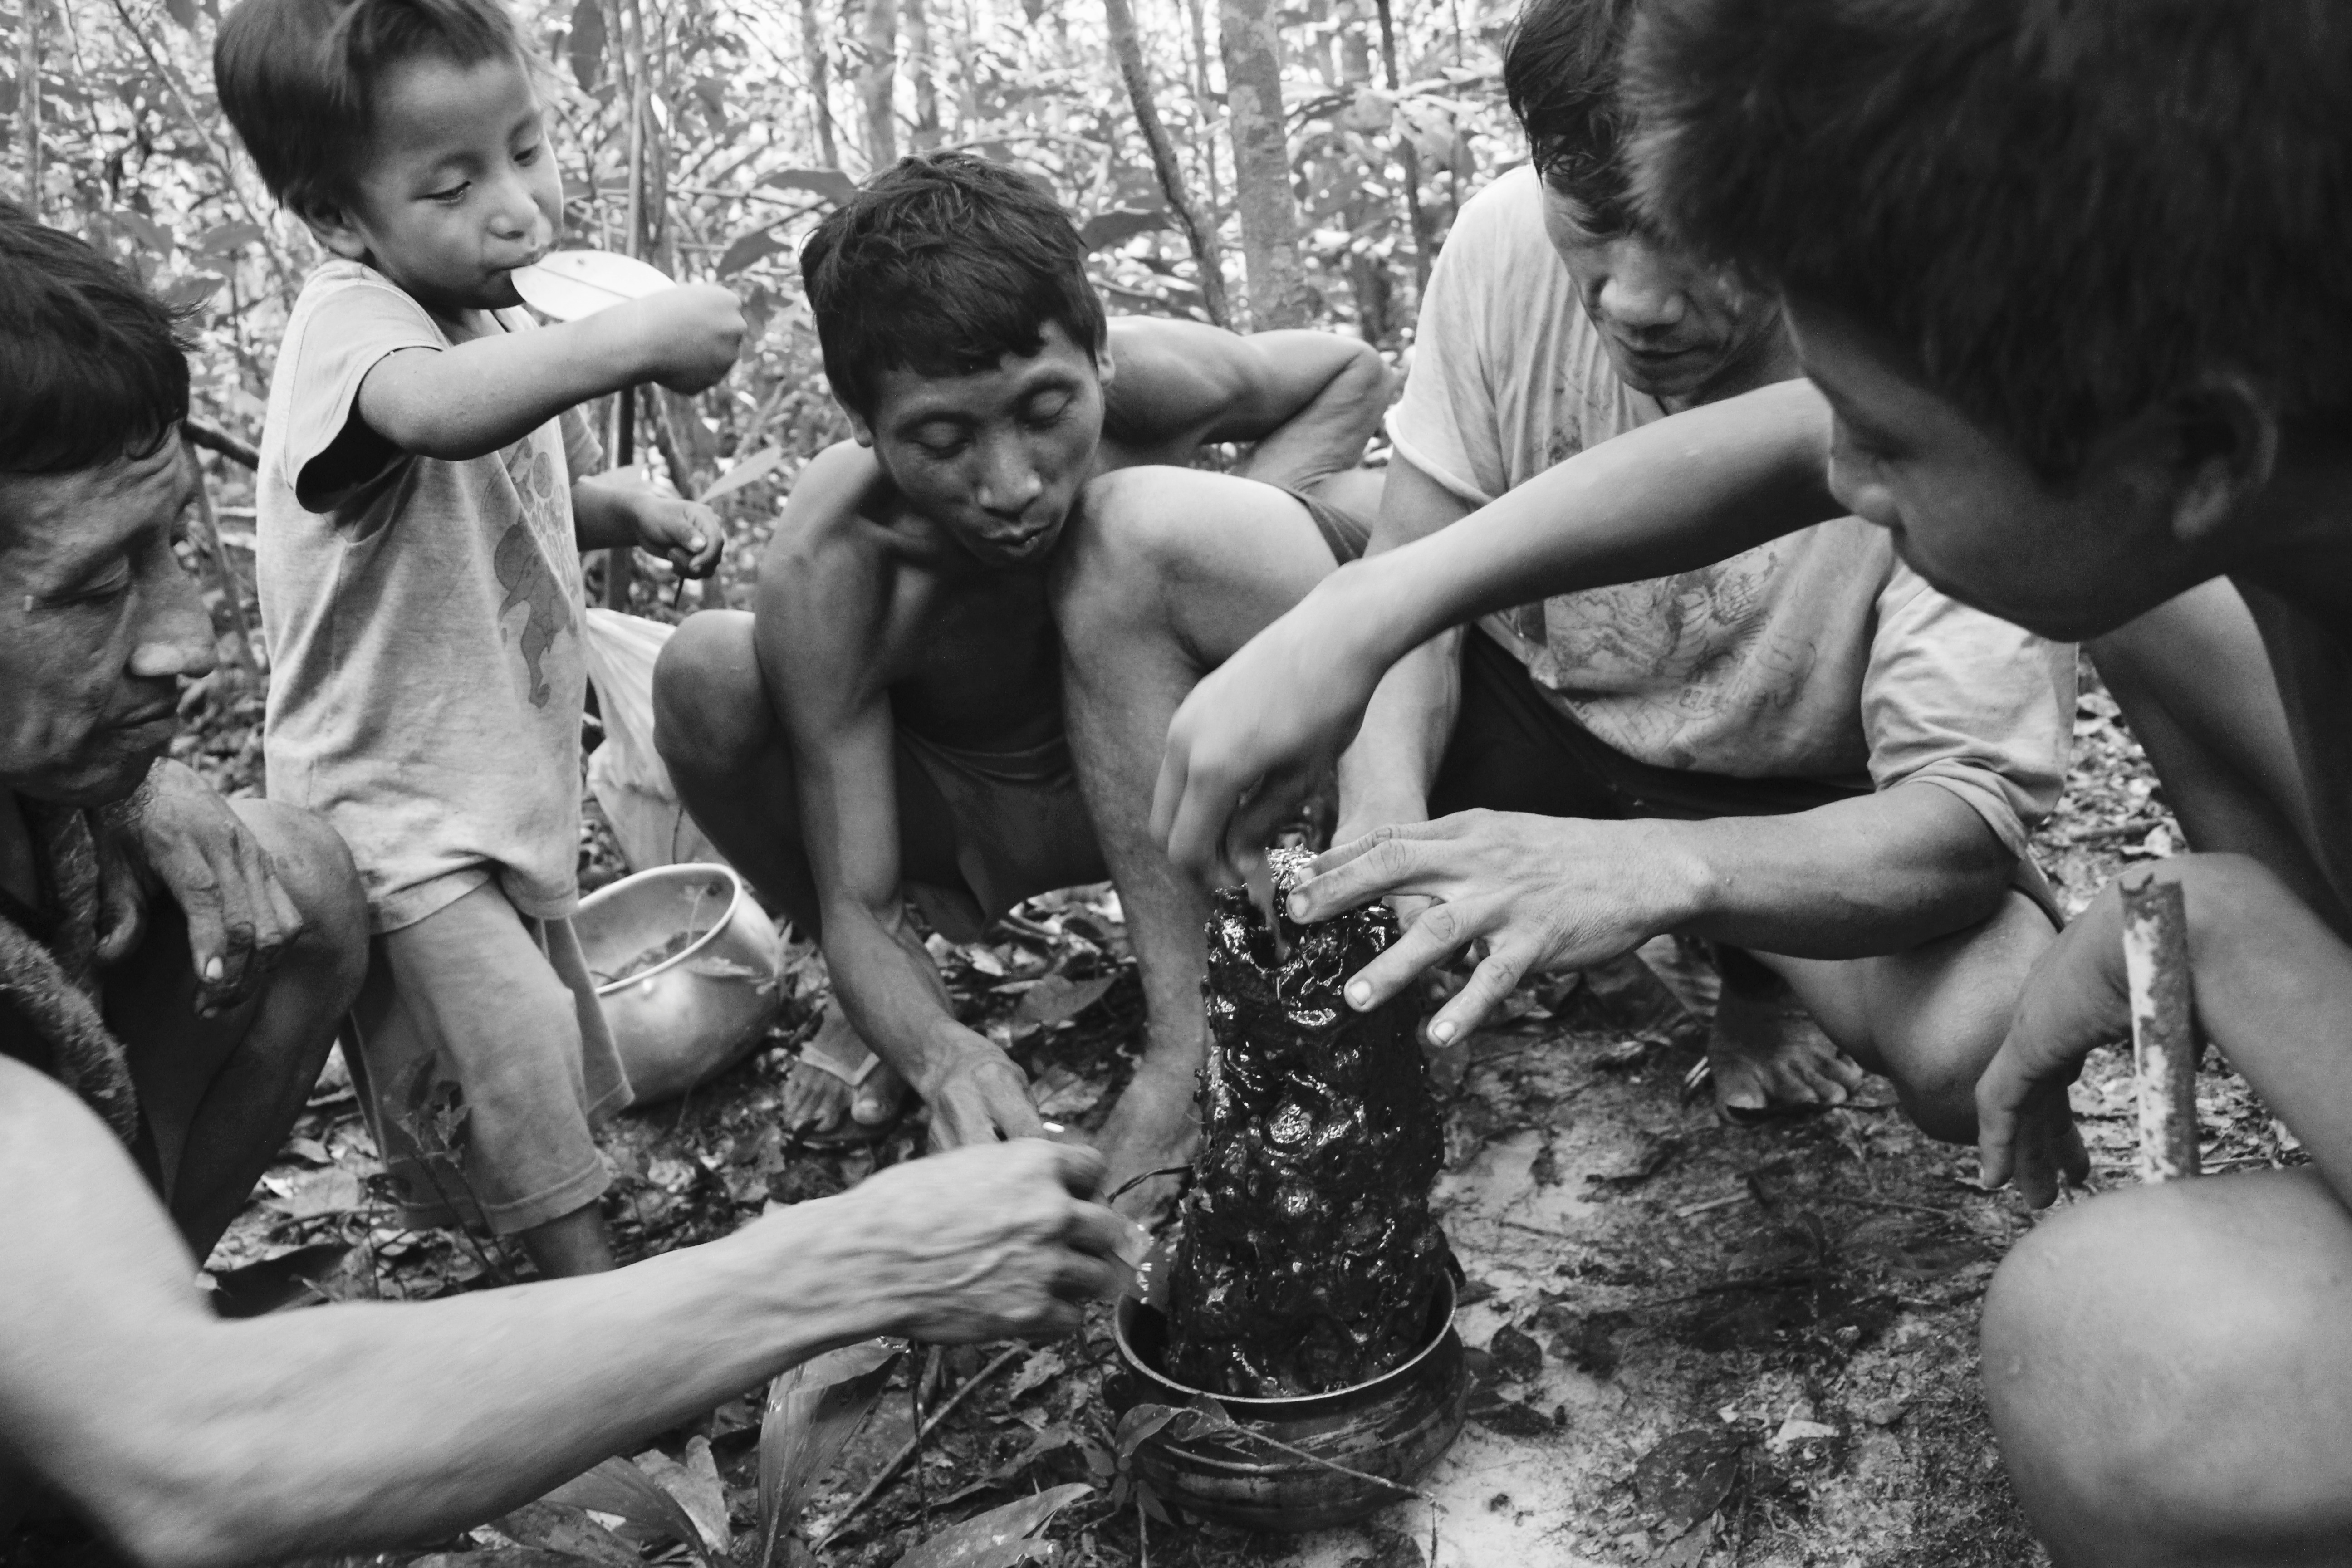
\includegraphics[width=\textwidth]{./imgs/IMG_1672}
%\caption{Takamỹxa'a, seu filho Warara’ia com a folha de mel na boca, Majhuxa’a, Hajkaramykỹa e seu filho Warajua se refastelando de \textit{hairaxĩa}, o mel da tartaruga capininga (acampamento de caça, aldeia Awá, 2013).}
%\end{figure}

Não apenas com alguns tipos de mel, mas com vários alimentos
--- \textit{hanimiũ'a} ``minha comida'' ---, as pessoas desenvolvem um elaborado
sistema de controle. Isso sucede sobretudo durante o pós-nascimento de
crianças --- \textit{wehẽ}, ``sair'' ---, menstruação, além de momentos como luto
ou doenças, que exigem atenção redobrada. As pessoas próximas (uma
família, por exemplo) se conectam de maneira consubstanciada, e a saúde
de um afeta diretamente a saúde de outro --- não muito diferente do que o
ocidente argumenta sobre os efeitos de um vírus, como o da gripe, ao
atingir um membro da família, com a potencial contaminação da família
inteira.

Os Guajá dizem não saber comer alimento ``amargo'', \textit{irawahy}, cujo
amargor quase sempre terá fins medicinais. Apesar de gostos azedos, 
\textit{hajahy}, figurarem na dieta Guajá, ainda não ``aprenderam'' a comer
amargo, como disse um amigo certa vez, ao explicar-me a intolerância a
esse sabor. Dos procedimentos para proteger a pessoa em situações
sensíveis, como das mulheres em menstruação --- ``estar sangrando'',
\textit{hawy} ---, a ingestão de uma infusão amaríssima feita com a casca de
uma árvore chamada \textit{mata'ya}, que não identifiquei, é muito
indicada por proteger as ``tripas'' --- intestinos e, nesse caso, também
fígado. Por exemplo, na primeira menstruação --- \textit{hawy}
\textit{mutuhũ}, ``primeiro sangue'' ---, a jovem deve tomar \textit{mata'ya}
para proteger o fígado e não passar mal com os alimentos. Miúdos em
geral, como fígado, vísceras e outros, estão proibidos. As mesmas
restrições alimentares recaem sobre mulheres menstruadas, além de homens
e mulheres em resguardo pós-nascimento. Vejamos alguns desses alimentos.
%\subsection{Principais alimentos proibidos a mulheres menstruadas ou mulheres e homens em resguardo pós-nascimento}                                                                                                                                                 
\begin{enumerate}
\item Ovos de jaboti, \textit{kamixa ripiakera}
\item Ovos de jacaré, \textit{jakare ripiakera}
\item Jaboti fêmea (o macho pode)
\item Carne de jacaré
\item Peixe surubim
\item Piranha
\item Peixe curimatá
\item Peixe traíra
\item Fígado e vísceras em geral
\item Macacos adultos
\item Paca
\item Queixada
\item Galináceos como jacamin, inhambu e mutum
\item Veado mateiro, \textit{arapaha}
\item Veado foboca, \textit{arapaha'ia}
\item Pequiá ou pequi,\footnote{\textit{Caryocar villosum}.} \textit{myky'a}
\item Pelo menos seis tipos de mel
\end{enumerate}

Quando nasce um filho, nem o marido nem a esposa podem beber água por
uns dias, e o mesmo ocorre com a mulher menstruada. Só é permitido beber
\textit{mata'ya}, essa infusão de madeira amarga, e deve-se dormir
bastante. Por isso o resguardo é chamado de ``o descanso das pessoas'', 
\textit{awa nypyate hakeri}. Até o cordão umbilical cair não se come
praticamente nada, e toda a dieta deve ser observada após a queda do
``umbigo'', \textit{iporowãena}. Pequenos peixes como mandi e sardinhas são
indicados, assim como a carne de animais pequenos, como as cotias. Nesta
época, a carne de macaco, alimento muito apreciado, só pode ser
consumida se for de animais jovens, preferencialmente de capelães.
Frutos como inajá, bacaba, açaí, cupuaçu, bacuri e cacau podem ser
consumidos, bem como animais como a cotia e o tatu. O tatu, inclusive,
tem uma carne indicada para consumo em períodos de fraqueza pois, assim
como o couro do tatu é duro, sua carne fornece força e dureza, \textit{hatỹ}, 
para quem a come. Nesses períodos só se podem consumir
jabotis machos, já que um dos riscos mínimos da mulher que ingere carne
de jaboti fêmea seria dar à luz filhos com problemas de pele, e o risco
máximo seria dar à luz jabotis. Para a proibição do consumo de diversos
alimentos, os Guajá dão explicações relacionadas aos possíveis efeitos
negativos no corpo do bebê ou dos pais. Peixes como o curimatá, \textit{mykukyruhua}, 
e a traíra, \textit{tara'yruhua}, devem ser evitados,
pois podem gerar feridas no corpo da criança. A carne de ``jabotas'' ---
as jabotis fêmeas ---, por exemplo, é lembrada por produzir cansaço nos
homens, que não aguentariam subir as ladeiras da mata. Nesta época só
comem jabotis machos.

Quanto às dezenas de méis que ainda veremos neste livro, adianto que
eles são alimentos muito apreciados e amplamente consumidos, mas podem
ser também muito perigosos. Os méis em geral são alimentos ``quentes'' que
causam \textit{emoção} a quem consome. Sua doçura faz bem à saúde, mas
algumas espécies podem ser nocivas em períodos de resguardo:

\begin{enumerate}
\item \textit{Iramuira}, mel do inhambu, causa febre
\item \textit{Kamixaira}, mel do jaboti, causa coceira no corpo
\item \textit{Mu'uira} causa atrofia nos dedos das mãos e pés
\item \textit{Tataira},\footnote{\textit{Oxytrigona tataira tataíra}.} abelha caga-fogo, causa queima a pele da criança
\item \textit{Pirairuhua} causa calafrios em pais e filhos
\item \textit{Uhua}, mel da anta/\,abelha \textit{xupé},\footnote{\textit{Trigona hyalinata Lepeletier}.} causa efeitos não identificados
\end{enumerate}

O consumo do mel \textit{iramuira}, ``mel do inhambu'', para a mulher
menstruada ou em cuidados pós-parto provocaria o endurecimento de seu
intestino. Hajkaramykỹa me contou sobre uma mulher no passado que comeu
desse mel enquanto estava menstruada, e seus órgãos internos, o
intestino em particular, ``secaram''. Ela ficou entupida sem conseguir
urinar ou defecar e morreu.

No caso de um resguardo menor, por menstruação, os cuidados não recaem
no marido e filhos. Veremos ainda que os Guajá compartilham a
paternidade, pelo que crianças têm mais do que um \textit{pai}, e os
cuidados pós-nascimento --- todo o sistema de \textit{resguardos} que
restringe a alimentação e atividades --- recaem não somente sobre o marido
da mãe, mas sobre todos os outros que são considerados genitores da
criança e, muitas vezes, os irmãos do pai (\textsc{fb}). Embora as mulheres
experimentem essas interdições de maneira periódica --- mensalmente, os
homens, por sua vez e apesar de bem menos, as experimentam não só quando
nascem seus filhos com sua esposa, mas qualquer outra criança que ele
tenha ajudado a conceber.

Em geral, não há consumo de carne que fique impune. Nesses períodos os
homens sequer devem sair para caçar, e nem homens nem mulheres devem
mexer com caça no sentido de ``limpar'', \textit{hape}, o animal: despelar,
tirar vísceras, cortar, cozinhar. O resultado imediato são dores de
cabeça, \textit{jakỹ wakyhy ta}, e febre em pais e filhos. A mesma dor de
cabeça ocorre se qualquer um da família consumir macacos adultos. Todas
as atividades de caça são interrompidas, e um homem só poderá abrir
exceção, sob muito cuidado, caso tenha outras bocas para alimentar --- se
seus filhos estiverem com fome. Diversos animais podem ser capturados
enquanto o bebê não ``mexer o pescoço'' com autonomia --- ou seja, se não estiver
ereto ---, tais como veado-mateiro e veado-foboca. Ainda assim, por
exemplo, não se matam machos das espécies macaco-prego, cairara, ou
quatis, pois provocam até enlouquecimento. Mesmo as fêmeas não são
consumidas, são capturadas apenas para aplacar a fome das crianças.

Seja na \textit{couvade} ou fora dela, comer carne, \textit{ha'okera}, é
algo sempre perigoso --- devido a ``raivas'' e vinganças que os animais
podem lançar sobre quem os caçou ---, e alguns animais em particular são
perigosos sempre, como parece ser o caso do veado mateiro, \textit{arapaha}. 
Carnes como a de veado, apesar de amplamente
consumidas, sempre provocam revertérios por serem ruins, ``reimosas'',
\textit{manahỹ}. Quando a mulher de Tatuxa'a deu à luz a pequena
\textit{Iwapanỹ}, ele foi caçar --- esperar --- um veado mateiro na floresta,
sem que o cordão umbilical da menina ainda tivesse caído. Ele o fez,
pois seu outro filho, Takwarary, estava ``chorando de fome'', pedindo-lhe
carne para comer, e os homens Guajá sempre vão caçar quando seus filhos
estão clamando por comida. Por isso ele resolveu ``esperar'', \textit{matakwa}, 
o veado à noite. Sua caçada foi bem-sucedida, ele
conseguiu matar três cotias a caminho da espera e um veado mateiro
durante a noite. No dia seguinte retornou à aldeia, e no mesmo dia sua
filha recém-nascida contraiu uma febre alta que não passava. Tiveram que
retirá-la da aldeia com o carro da \textsc{sesai} e enviá-la para o hospital na
cidade de Santa Inês. Segundo Tatuxa'a, sua filha quase morreu. Além de
atribuir a doença da filha recém-nascida ao fato de ter ido caçar veados
no momento que deveria estar descansando em casa, o homem também
comentou que, se tivesse matado uma onça, certamente sua filha estaria
morta hoje.

A onça é um animal perigoso de matar. Os Guajá gostam da carne de
sussuarana, a onça parda; lembra-lhes o sabor da carne de veado. E mesmo a
onça-pintada podia ser consumida, ao menos ``antigamente'', lembram as
pessoas. Porém, de todas as restrições em período de cuidados
pós-nascimento, mas também durante menstruação e doenças, não se deve matar, e
muito menos consumir, carne de sussuarana ou de qualquer outra onça, pois
provocará a morte do bebê. No caso da onça, a proibição de matar se
inicia na gravidez e segue até o pós-parto. Caso um homem mate o felino
durante esse período, além da morte do bebê, a própria grávida ou mãe
poder morrer ou seu leite secar. O seio da esposa pode sumir, tornando-a
``lisa'', ``como se tivesse o peito de um homem'', alertou-me certa vez
Hajkaramykỹa. Em um relato de seus diários de campo, a pesquisadora Rosana Diniz escreve:

\begin{quote}
Nesse sentido, Hajmakoma'ã me fez o seguinte relato, em 2010: tinha ido
caçar e encontrou com uma onça, mas esta o viu primeiro. Então, ele se
pôs a correr na floresta, e a onça atrás. Chegando em um rio, ele
jogou-se na água e a onça, então, desistiu da perseguição. E porque você
não atirou nela? Perguntei. Ele respondeu: e minha filha pequena,
\textit{xikari} (minha irmã)? Não posso matar onça, faz mal para a minha
filha, ela pode morrer.\footnote{Diniz, 2015, pp.\,55--56.}
\end{quote}

A quebra do resguardo de nascimento, de acordo com Hajkaramykỹa, atinge
a todos da casa, e por determinados animais, caso das onças, a escolha
em caçar e/\,ou comer pode ser mortal. Pai, mãe, filhos, irmãos e pessoas
ligadas à casa estão relacionados e, por sua vez, se conectam a
diferentes subjetividades --- animais, vegetais ou espectrais --- que vivam na
floresta. Por isso, vômitos e fezes dos bebês não podem ser abandonados
nem no chão da aldeia, pois são comidos por cachorros, nem na floresta,
pois são comida de animais, principalmente os gambás, jabutis,
carrapatos e marimbondos, sob o risco de adoecimento ou morte do bebê.
Esses excrementos --- para não ser consumidos por animais --- também não
podem ser enterrados para não virarem ``comida de minhoca''. Caso as
minhocas, \textit{amirikuria}, --- ou qualquer outro animal --- o comam, os
bebês adoecem. O tratamento mais comum é envelopar essas fezes em folhas, 
como a folha de \textit{akareho}, por serem planas, e a amarrar com
cipozinhos, como pedacinhos de ``cipó titica'', por exemplo, deixando
pendurados em alguma árvore, livre do alcance de todos os bichos. Esses
``embrulhos'' são chamados \textit{ximixia}. Não podem ser jogados fora,
nem enterrados. Devem ficar pendurados até as fezes apodrecerem
--- \textit{ipiru}, ``podre''.

%\textbf{Foto de ximixia}
%\begin{figure}[H]
%\centering
%  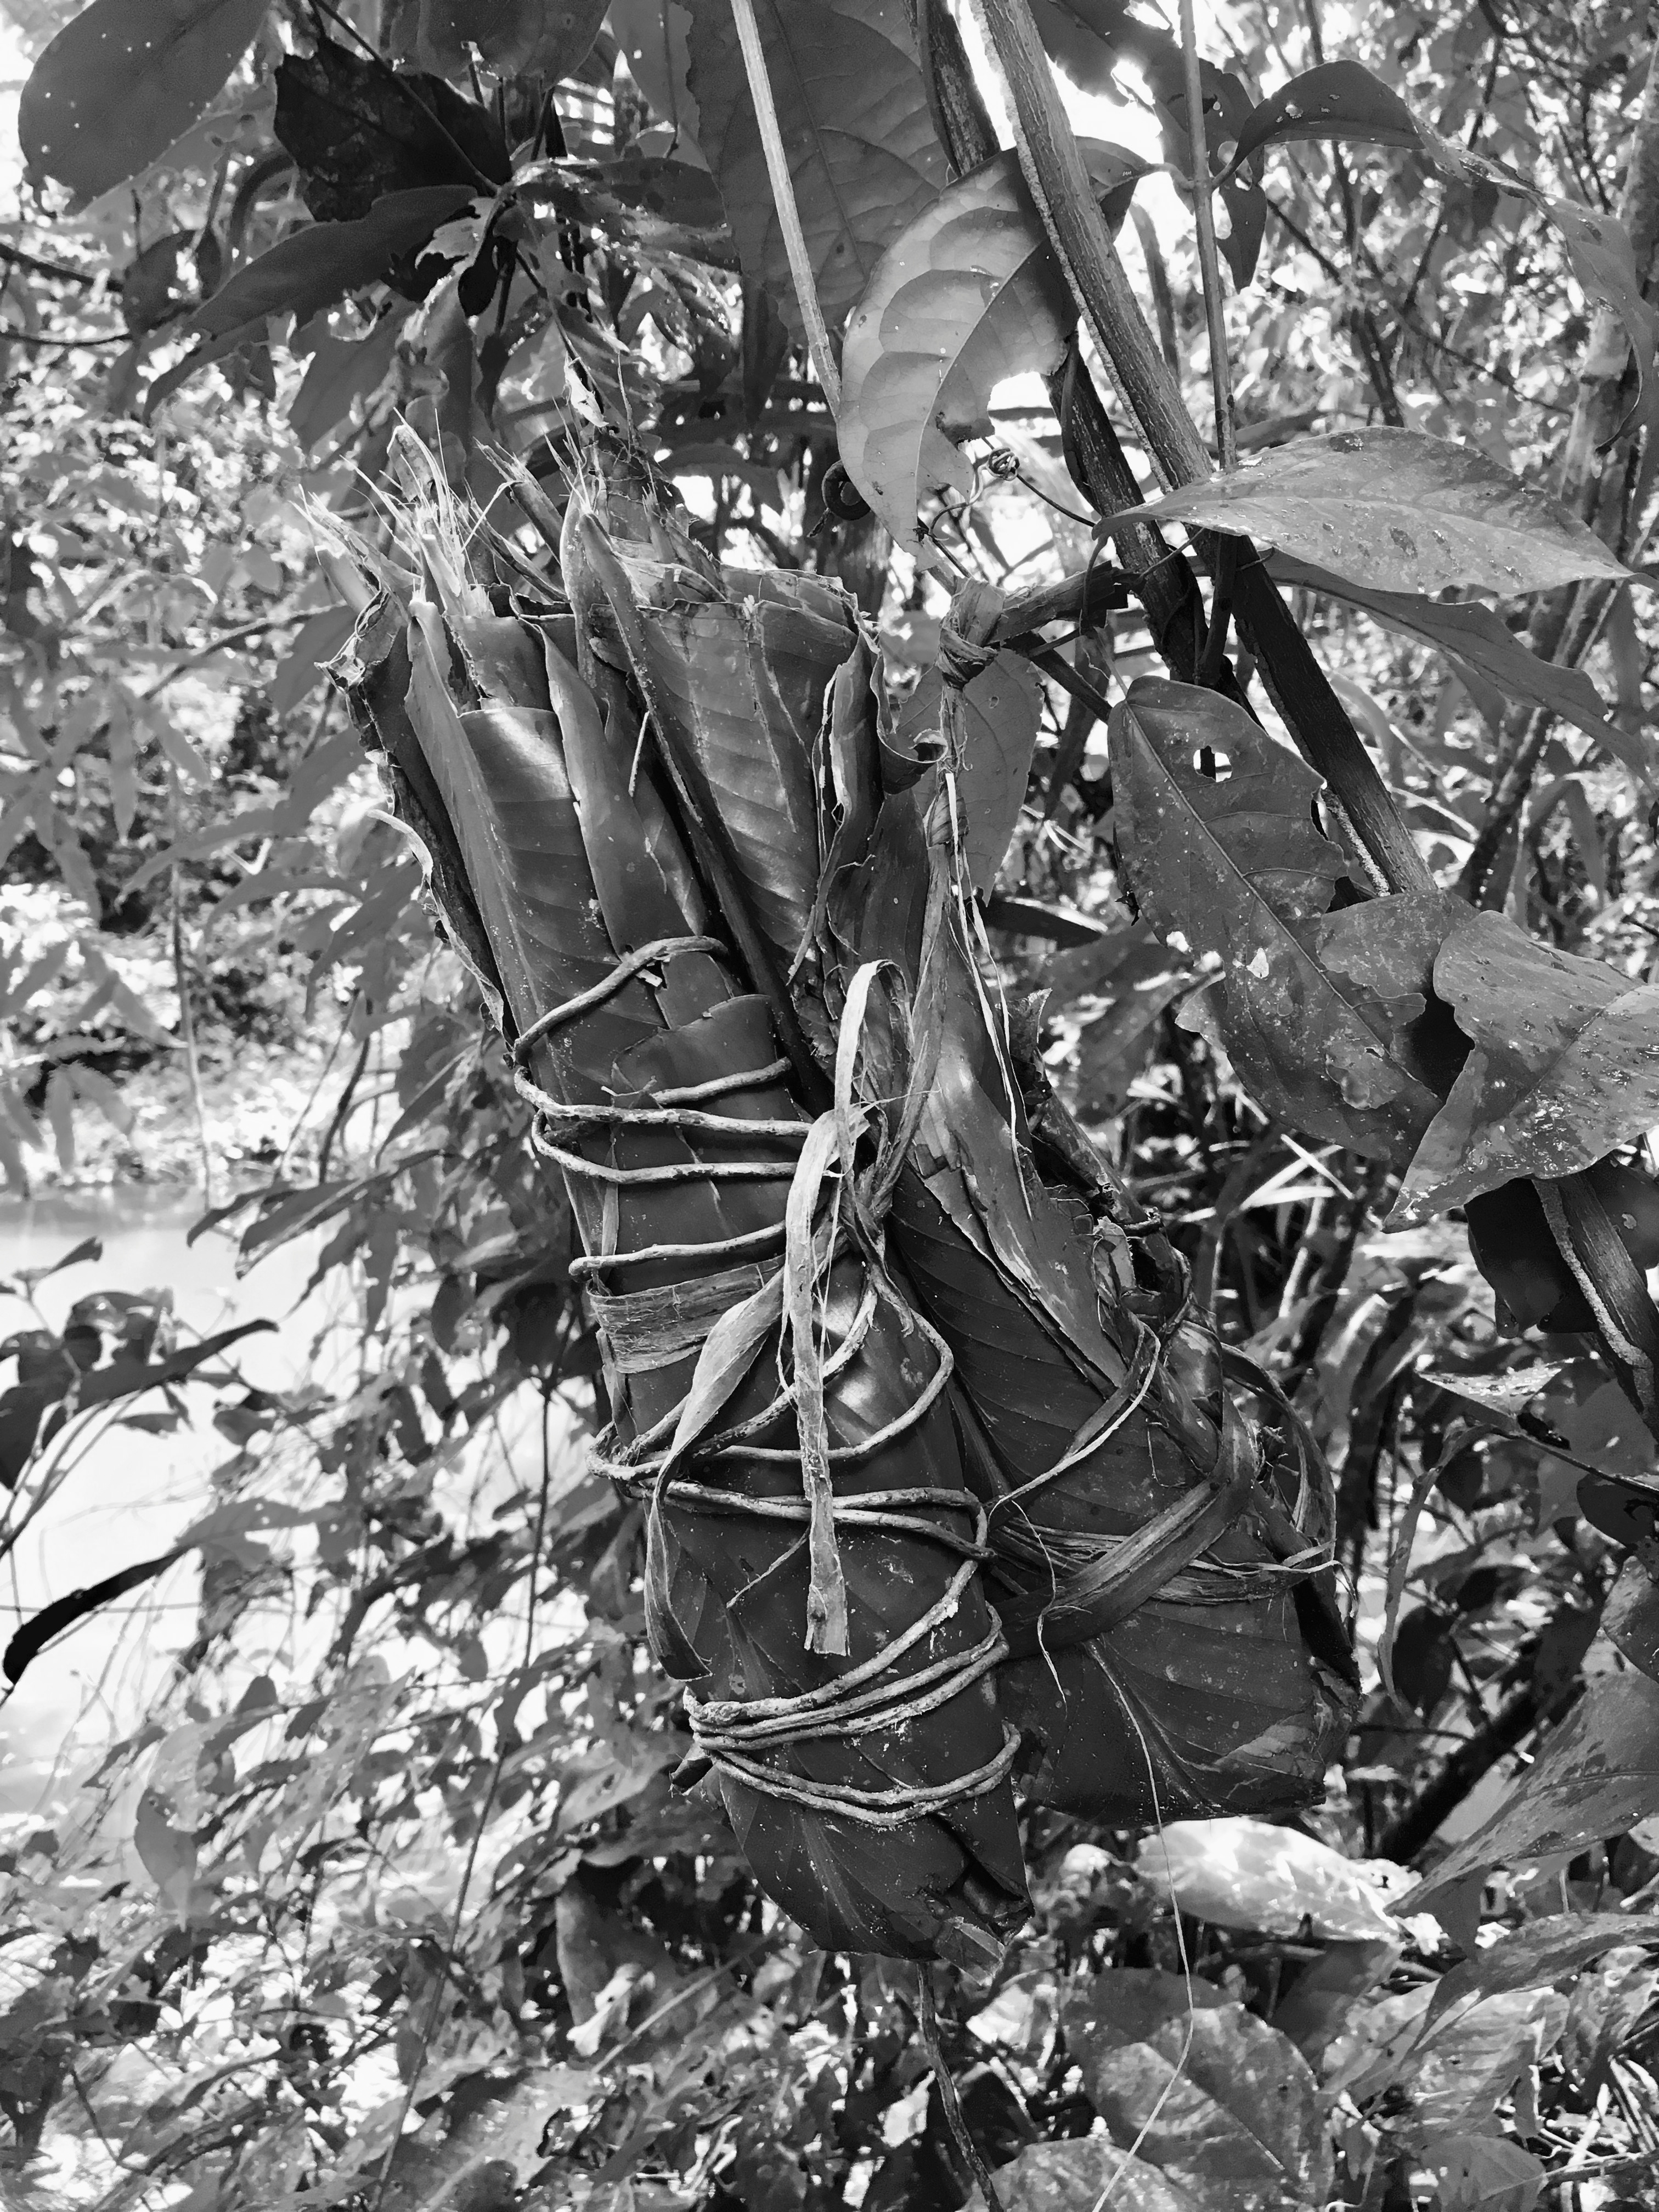
\includegraphics[width=\textwidth]{./imgs/IMG_4613}
%\caption{Ximixia feita por Jawatara'ia e pendurada no caminho da aldeia após o nascimento do seu filho (aldeia Juriti, 2018).}
%\end{figure}

Diversos cuidados também devem ser observados no manuseio dos alimentos.
Apenas como um exemplo, ossos de machos de espécies de macacos como o
cairara, \textit{Cebus kaapori}, e macaco-prego, \textit{Cebus apela}, não
devem ser atirados no chão para que não entrem em contato com ninguém.
Em se tratando desses ossos, o perigo é algo próximo da feitiçaria, chamada 
pelos Guajá de \textit{ma'akwá}. Os ossos de fêmea, porém, não
carregam feitiço. Ao consumir macacos desse tipo, seus ossos devem ser
separados da carne antes de os pais os darem aos filhos, para que as
crianças não os arremessem em alguém ou algum lugar.

Por outro lado, apesar de mencionar aqui a ideia de ``regras'' e
cuidados, da forma pela qual esses resguardos são pensados, as pessoas
nunca falam em interdições, e muito menos em regras, propriamente. Se
existem resguardos, é porque também existe uma possibilidade real, um
desejo em sair para caçar, seja para matar a fome, \textit{nahakatãj}, dos
filhos maiores ou outros parentes, seja para acompanhar os amigos por
pura vontade de matar bichos. É muito comum pessoas ligadas ao pai em
resguardo chamarem-no para caçar, insistindo até para ele descumprir seu
período de reclusão. Este quase sempre deve dizer que ``está cansado para
caçar'' ou ``tem que ficar com seu filho'' ou mesmo que ``sua mulher não
quer ficar sozinha''. Mesmo em mudança na alimentação e nos hábitos, o
homem em reclusão não insinua isto de maneira tão explícita em suas
falas. Os argumentos evocados para ele permanecer em sua casa (ou mesmo
em sua rede) são sempre mais ``prosaicos'' do que a ideia de ``resguardo''
ou ``regras''. Preferem dizer: ``Vou ficar em casa olhando meu filho!'', e
essa frase resumiria tudo.

Por fim, podemos pensar que as proibições e interdições de dieta para as
mulheres e homens que esperam ou tiveram filhos recentemente só são
realmente conhecidas por seus efeitos, como já discutido por Coelho de
Souza (2004, p.\,44), apesar de todos os \textit{a priori} que enumerei
acima. Por exemplo, as mulheres da aldeia Juriti não comiam carne de
veados --- mateiro e foboca --- e galinha ou frango, sob o risco de terem
fortes sangramentos. Apenas nos últimos anos (2011/\,2012), quando pessoas
de outras aldeias --- cujas mulheres consomem carne de veado --- começaram a
manter contatos mais intensos com os Guajá da aldeia Juriti, elas
passaram a comer carne de veado, caso não estejam menstruadas, e, de
maneira geral, tal ``proibição'' caiu. Nas viagens para a cidade em
reuniões e encontros, que são cada vez mais frequentes na vida dos
Guajá, a observação dessas regras é motivo de debates entre maridos e
esposas. Certa vez, Jauxika, que estava grávida de oito meses, proibiu
seu marido Takwari --- que estava indo para uma reunião em outra aldeia ---
de comer carne de frango, até que o pai de Takwari, Pira'ima'ã,
interveio e disse que quando sua esposa esteve grávida e ele foi à
cidade, comeu carne de frango, e nada de mal aconteceu a ele. Jauxika, a
mulher, ouviu com interesse a explicação do homem e então disse para
Takwari que ele podia, sim, comer carne de frango e gado, mas devia
prestar atenção para não passar mal. Mas que não comesse, de forma
alguma, carne de porco, do mato ou dos brancos, pois isso faria mal a
ela e ao bebê. Os alimentos específicos que podem ou não ser consumidos
são sempre debatidos a cada nova gravidez, a cada nova situação de
restrição. Ainda que haja esse conjunto que aqui destaco e costuma
sempre ser observado, as interdições sempre serão compreendidas pelos
efeitos e resultados de determinados alimentos no corpo dos sujeitos,
seja uma pessoa ou uma família com que se afetam mutuamente.

Embora não seja meu tema de pesquisa, finalizo este tópico anotando que
os Guajá desenvolveram uma infinidade de medicamentos, \textit{pohỹ}.\footnote{Também denominados \textit{ira pohỹ}, ``remédio das
  árvores''.} muito eficientes no combate a muitas doenças\footnote{Ver o
  artigo de Cormier (2005) em que a autora traça um perfil mais
  detalhado daquilo que ela denomina ``simbolismo vegetal'' dos Guajá,
  apresentando um conjunto bem mais amplo de doenças e relacionando-as à
  concepção Guajá de pessoa e morte. Ainda no tratamento da etnobotânica
  dos Guajá, o trabalho de Balée (1994) é sem precedentes.} Mesmo
guardando um grande fascínio pela etnomedicina dos \textit{karaia}, com
seus comprimidos, pomadas e injeções, a que recorrem sistematicamente,
os Guajá fazem uso de ambos os remédios, dos \textit{awa} e dos
\textit{karaia}, em diversas situações. Por exemplo, quando o rapaz Juxa'a
foi picado por uma cascavel e, na enfermaria do \textsc{pin}, lhe aplicaram
algumas doses de soro antibotrópico, sua mãe aplicou-lhe em cima da
picada um emplastro feito com uma casca de árvore chamada
\textit{hiratanỹ} a fim de expulsar o veneno da cobra. Muitas dessas
folhas, cascas e cipós têm nomes de animais que são seus \textit{jara}, ``donos''. 
Vejamos alguns desses medicamentos. Para salvaguardar a
propriedade e o conhecimento sobre essas plantas, omito os nomes nativos
substituindo-os pela sigla \textsc{p}, de \textit{planta}, seguido de um número:

\begin{itemize}
\item\textbf{\textsc{p1}}\quad Folha que se amassa a fim de tratar dores
musculares, dentre outras dores. Passa-se nos braços e articulações, em
aplicações periódicas, e é capaz de expulsar tais dores. Também
utilizada contra febre, pode ser ingerida após macerada, \textit{jamixo},
e adicionada a água e mel
\item\textbf{\textsc{p2}}\quad Folha\footnote{Algo que pode ser traduzido como \textit{veado vegetal}.} que os Guajá esquentam na fumaça do moquém, colocando-a em
seguida nas pernas, nádegas e costas para debelar a febre. Um
antitérmico
\item\textbf{\textsc{p3}}\quad Com muitas utilidades, esta entrecasca também é
chamada \textit{irawahy}, ``amargosa'', e tem como função tratar dores no
fígado, estômago e vísceras. Pode ser utilizada em forma tópica,
colocada sobre o abdômen da pessoa em repouso. Se o enfermo tiver
vômitos, é ingerida macerada misturada com mel e água, de modo a
amenizar o gosto amargo. Após o nascimento de uma criança, seu pai deve
ingeri-la macerada, com a finalidade de proteger seu fígado
\item\textbf{\textsc{p4}}\quad Utilizada contra dores de cabeça, esta folha é
muito cheirosa. Se macerada, pode ser aplicada durante os banhos no rio.
Após alguns dias de aplicação a dor se esvai.
\item\textbf{\textsc{p5}}\quad De função idêntica à \textit{Henemy ka'y}
\item\textbf{\textsc{p6}}\quad Folha\footnote{Uma tradução possível é \textit{mel vegetal}.} de
cheiro agradabilíssimo, cuja função é espantar dores de cabeça e no
corpo. Utiliza-se esfregando-a nas partes afetadas
\item\textbf{\textsc{p7}}\quad De uso e função parecida da \textit{Haira Ka'a},
porém só aplicável a dores de cabeça
\item\textbf{\textsc{p8}}\quad Entrecasca de uma árvore cuja seiva alivia as dores
de ferida e queimaduras, além de ajudar na cicatrização de ferimentos
externos
\item\textbf{\textsc{p9}}\quad Folha utilizada contra a febre. Utiliza-se
esfregando-a no corpo
\item\textbf{\textsc{p10}}\quad Frutinha cheirosa de cor amarela, de uso tópico;
esfregam-na no corpo a fim de expulsar dores e febre
\item\textbf{\textsc{p11}}\quad Casca de uma árvore, com o mesmo nome. Se inalada,
seu cheiro mentolado combate febre e calafrios
\end{itemize}

Esta é uma pequena amostragem de medicamentos que atuam contra as
doenças que atacam o \textit{hajtekera} e, por consequência, os
componentes vitais de uma pessoa.\footnote{Para uma boa análise da etnomedicina
Guajá, consultar Cormier, 2005.}

\section{\textit{ha'aera} e \textit{ajỹ}, «morte» e «fúria»}

O último elemento constituinte da pessoa Guajá, que apresento aqui, é o
\textit{ha'aera}.\footnote{O termo correto é \textit{a'a}; \textit{h-a'a-er-a}
  é o resultado da junção do prefixo de 3ª pessoa \textit{h} mais
  ``espectro'', ``raiva'' \textit{a'a} mais sufixo de a.n. retrospectiva \textit{er} mais sufixo nominal \textit{a}; porém os Guajá nunca se referem a
  \textit{ha'aera} como \textit{a'a}, sempre o fazem utilizando o sufixo \textit{era}
  ou \textit{e}, nas formas \textit{ha'aera} ou \textit{ha'ae} (a depender da
  construção da frase).} Os Guajá traduzem tal palavra para o português
por ``raiva'', não se tratando da mesma ``raiva'' expressa pelo termo
\textit{imahy}. \textit{Imahy} é um sentimento que, apesar de perigoso e
desprezado, é muito comum e desejável em diversas situações, como na
guerra. \textit{Ha'aera} pode ser traduzido pela ideia de
``raiva-espectro'', devido tanto à sua condição de ``sombra'', ``alma'' bestial,
liberada após a morte --- processo cuja consequência é a transformação em
um ser que é pura ``raiva'', os \textit{ajỹ} ---, pelo fato de o \textit{ha'aera}
atuar durante a vida como um dos componentes da pessoa humana. Para
melhor definição do termo, podemos contrastar o \textit{ha'aera} com o
\textit{hajtekera}, sendo este último um princípio que agencia a vida,
enquanto o \textit{ha'aera} agencia morte, dores e sofrimentos.

O \textit{ha'aera} é uma substância constitutiva do próprio ser: ``Está por
aqui!'', me disse certa vez Wiraho, apontando para seu peito e barriga.
Humanos e alguns animais possuem \textit{ha'aera}. E no caso dos animais é
essa potência que atormenta os humanos na forma de vingança após as
caçadas --- a qual emana doenças e retira a sorte em caçadas futuras. No
caso particular da constituição da pessoa, o \textit{ha'aera} é aquilo que
diversos autores chamariam de ``espectro'' de um morto.\footnote{Ver \textit{Jurupari
-} Waiãpi, Gallois, 1988, p.\,178).} Uma vez morta, as partes da pessoa se
desfazem: o \textit{ipirera} apodrece na terra; o \textit{hajtekera} se
encaminha para o \textit{iwa}; e o \textit{ha'aera} se transmuta em
\textit{ajỹ}.

O \textit{ha'aera} não é só o espectro de um morto recente, uma sombra da
pessoa morta que um dia se transformará em \textit{ajỹ}, ele é uma
substância que também compõe a vida e que só após a morte vaga como
``alma penada'' e se mescla à massa de seres \textit{ajỹ}, que são
dependentes do \textit{ha'aera} para viver. Não é possível afirmar que o
\textit{ha'aera} tenha uma aparência. Ao contrário, os Guajá definem
literalmente como uma substância, algo espectral. ``É como o seu
repelente!'', me disseram certa vez, um agente que tem poder de
penetração tão capilar como um gás. É algo que todo humano carrega, pois
faz parte da composição física humana, porém, liberado violentamente
após a morte, funcionando como uma energia formadora de seres ligados à
morte, os \textit{ajỹ}. A constante ameaça aos humanos que emana dos
\textit{ajỹ} é dita como \textit{ajỹ} \textit{ha'aera}, já que os \textit{ajỹ}
dominam esse princípio mortal, lançam-nos nos humanos fazendo-os adoecer
e até morrer. Os \textit{ajỹ} são constituídos pelo \textit{ha'aera} de
ex-humanos, por isso mesmo, em diversas situações, podem simplesmente
ser denominados \textit{ha'aera}, tal como um sinônimo. O \textit{ha'aera}
também pode ser chamado de \textit{ajỹ karawara}, já que os \textit{ajỹ} a
manipulam da mesma forma que os homens Guajá fazem com os
\textit{karawa(ra)}, as potências celestes que auxiliam os humanos em suas
curas. Em outras palavras, o \textit{ha'aera} é o \textit{karawara} dos
\textit{ajỹ}. Seres como os \textit{ajỹ} talvez sejam dos que mais
apareceram nas etnografias Tupi-Guarani desde os primeiros relatos de
viajantes, e permanecem como tópico importante até os trabalhos
atuais.\footnote{Para um balanço comparativo de noções parecidas a essa,
  como \textit{Anhang}, \textit{Aignan}, \textit{Anhanga}, dentre outras, cuja
  precedência na literatura etnológica é ampla, ver Viveiros de Castro
  (1986, p.\,255).} Porém, vejamos o que os Guajá têm a dizer sobre
eles.

``Seres pequenos, com a estatura de crianças e muito feios!'' Essa é uma
das formas de definir os \textit{ajỹ}, entidades que habitam antigos
acampamentos, ocos de árvores, buracos e áreas escuras da floresta. São
capazes de tirar a vida de alguém com um simples toque. Somente por
pressenti-los, uma pessoa pode entrar em estado febril. Da mesma forma,
são como ``curupiras'', que atrapalham cotidianamente a vida dos
caçadores, provocam doenças, mortes, além de serem \textit{jara}, ``donos'',
``controladores'', de um expressivo número de animais. Os Guajá atribuem
muitas de suas desventuras e azares na caça, \textit{panemuhũ}, aos
\textit{ajỹ}. Diferentemente dos Ka'apor ou dos Araweté, as figuras do
\textit{koropí} (Viveiros de Castro, 1986, p.\,244) ou \textit{curupir}
(Huxley, \textit{op.\,cit.}, p.\,205) estão ausentes do mundo \textit{awa}; são os
\textit{ajỹ} que desempenham esse papel de seres controladores de alguns
animais de caça, capazes, inclusive, de perseguir um caçador
lançando-lhe \textit{ha'aera} e deixando-o \textit{panemuhũ} --- ``panema'', sem
sorte ---, como veremos mais à frente. Os Guajá recolocam a figura
Tupi-Guarani do \textit{curupira}, com suas formas e atitudes específicas,
nos \textit{ajỹ}: aparência feia, monstruosa; domínio sobre algumas
espécies animais; hábitos noturnos; ataque a caçadores, dentre outras.
Isso pode ser atestado ao observarmos o caso Waiãpi, em que o
\textit{kurupi} ou \textit{kurupira}, embora seja entidade ligada aos
\textit{añã} waiãpi, não se confunde com eles. Devido a sua feiura e dieta
canibal, o \textit{kurupi} é, nos waiãpi, associado aos \textit{añã}, também
chamado \textit{añã poro'õ}, ``o maligno que nos come'', \textit{añã'go
ka'apor}, ``o grande maligno da floresta'', e ainda \textit{añã Tapirã'i}, ``dono da sapopema''. 
De acordo com um xamã Waiãpi, ``Kurupira é a mesma
coisa que Jurupari'' (Gallois, 1988, p.\,136).

Se pensarmos que o \textit{ha'aera} dos Guajá pode ser comparado ao
\textit{Jurupari} waiãpi, ao mesmo tempo que os Waiãpi põem em sinonímia o
\textit{kurupi} e os \textit{añã} (seres comparáveis aos \textit{ajỹ} Guajá),
podemos afirmar que, ao contrário dos Araweté, Ka'apor
e Waiãpi, que convivem com a figura do \textit{curupira}, os Guajá
depositam as potencialidades deste nos \textit{ajỹ}: seres com caráter
múltiplo, de alma morta e protetores dos animais, dentre outras qualidades
possíveis. Além de provocar doenças e morte, os \textit{ajỹ} são seres com
os quais os Guajá constantemente estão sujeitos a encontrar,
principalmente porque alguns dos animais mais caçados pelos humanos são
de criação, \textit{nima}, dos \textit{ajỹ}. São eles: o veado mateiro, 
\textit{arapaha}, veado foboca, \textit{arapaha'ia}, cotia, \textit{akwixia}, 
paca, \textit{kararuhua}, e o quati, \textit{kwaxia}.
Esses devem ser caçados pelos humanos com comedimento e atenção, pois
onde estão podem também estar seus ``donos'', \textit{jara}, os \textit{ajỹ}.
Portanto, já não estamos somente no campo dos espectros e sombras, \textit{ha'aera}, 
mas sim no de seres que, assim como os \textit{awa} e os
\textit{karawara} celestes, detêm recursos de ``domínios'', \textit{riku}, 
sobre outros seres e se relacionam --- ainda que de forma infeliz --- com os
humanos.

Como habitantes da mata, os \textit{ajỹ} dominam uma série de seres,
situações e princípios, tornando a caçada --- para os humanos --- uma
atividade ainda mais perigosa e guerreira. Os Guajá dizem que podem
perceber a presença dos \textit{ajỹ}, pois sentem frio, \textit{haxỹ}, e
dores de cabeça quando tais seres estão próximos. Além disso, os
\textit{ajỹ} produzem um assobio longo característico --- pois é o único som
que sabem emitir --- e batem repetidamente no tronco das árvores com uma
grossa vara de madeira, ``um pedaço de pau'', a fim de dispersar os
animais. Em uma tarde, na aldeia Juriti, um homem chamado Hajmakoma'ã me
alertou para um assobio que ouvíamos ao longe: ``Você está ouvindo esse
assobio?'' ele me perguntou. ``São os \textit{ajỹ}!'' ele mesmo respondeu.
Sem entender direito sua afirmação, interpelei-o dizendo que se tratava
do canto de um pássaro e não do assobio dos \textit{ajỹ.} Ele concordou,
afirmando que tratava-se do cricrió, \textit{Lipaugus vociferans},
pássaro que é chamado ``\textit{ajỹ mixiura}'', um dos animais de criação, \textit{nima}, 
preferidos dos \textit{ajỹ}. Por isso, sempre que ouvem o
cricrió cantar, eles sabem que os \textit{ajỹ} estão por perto. O som do
cricrió é dito ser o próprio som dos \textit{ajỹ}, e este pássaro tem a
capacidade de se transformar em \textit{ajỹ}, tendo em vista que ele mesmo
o é. O mesmo ocorre com o canto do pássaro \textit{hakawỹ} --- acauã,
\textit{Herpetotheres cahinnans} ---, um canto causador de doenças pois
contém \textit{ha'aera}. Se um caçador ouvir seja o acauã, \textit{hakawỹ},
ou o cricrió, \textit{ajỹ mixiura}, enquanto estiver na floresta, pode ser
que não encontre caça alguma, pode ser que fique com febre, pode ser que
algo ainda pior aconteça, e pode ser que nada ocorra também. Em todo o
caso, ele deve fugir para longe do alcance do canto. Da mesma forma que
o gambá, ou mucura, cujo nome na língua guajá é \textit{ajỹ,} é um outro, 
e talvez o principal, avatar dos \textit{ajỹ}. Seu cheiro fétido é o
mesmo cheiro de morte exalado pelos \textit{ajỹ}. Muitos desses animais
são pura \textit{ha'aera} e, em diversas ocasiões, são chamados
``\textit{ajỹ}'', independentemente da forma que tenham. Quanto à sua dieta,
os \textit{ajỹ} se alimentam de jaboti, \textit{kamixa}, do quelônio
capininga, \textit{jaxaihua}, e de outro tipo de tracajá chamado
\textit{marapea}. Também comem inajá, \textit{inajã}, açaí, \textit{jahara},
bacaba, \textit{pinawã}, oiti, \textit{hixi}, além de vários frutinhos de
que os humanos não se alimentam, como a tatajuba, \textit{taryka}, e o
jatobá, \textit{itawa}, que os veados, pacas e antas comem --- pois os
\textit{ajỹ} apreciam a mesma comida que seus animais de criação.

Os \textit{ajỹ} contam com --- por assim dizer --- dois grupos de \textit{ajỹ
nima}, ``animais de criação''; um deles os humanos caçam e comem;
enquanto o outro os humanos desprezam por serem versões dos \textit{ajỹ}.
Por exemplo, o gambá, \textit{ajỹ}, e o macaco-da-noite, \textit{aparikya},
pertencem ao segundo grupo, enquanto a paca, \textit{kararuhua}, e o veado, 
\textit{arapaha}, ao primeiro. Vários tipos de sapos, \textit{kururua},
também são \textit{ajỹ nima}. Os sapos são animais pouco estimados e com
que não se quer muito contato, pois, segundo os Guajá, sujam as águas e
transmitem doenças. Da mesma forma, as corujas, \textit{pypya}, que são
vistas como \textit{ajỹ nima}, ``seres de criação'' dos \textit{ajỹ}, pois são
\textit{ajỹ wirohoa}, ``gaviões dos ajỹ''. A carne de coruja nunca é comida,
pois sabidamente enlouquece quem a consome. O macaco-da-noite, 
\textit{aparikya}, por exemplo, estaria para os \textit{ajỹ} assim como os
macacos em geral estão para os humanos, isto é, primatas que os
\textit{ajỹ} guardam muito gosto em criar em suas casas e fazem parte de
seu dia a dia. Quando à noite os \textit{ajỹ} saem a ``caçar'' --- \textit{wata},
``andar-caçar'' ---, vão acompanhados dos macacos-da-noite, tal como os
humanos durante o dia saem acompanhados de seus capelães, \textit{waria},
e macacos-pregos, \textit{ka'ia}, dentre outros.\footnote{Entre os
  Araweté, os macacos-da-noite são tidos como ``encarnações'' dos mortos
  (Viveiros de Castro, 1986, p.\,503); os Yudjá os consideram parte do
  conjunto dos seres \textit{ãwã} da floresta, ogros antropófagos (Lima,
  2005, p.\,188). Referências ao macaco-da-noite como animal que ``encarna'' a
  própria morte é vasta na bibliografia das terras baixas, e não cabem
  aqui maiores comentários.}

O domínio de seres análogos aos \textit{ajỹ} sobre diferentes animais de
caça é bastante difundido na Amazônia. Os veados e pacas,
particularmente, aparecem em diferentes contextos etnográficos como
animais cuja relação com a morte os torna uma carne ora evitada, ora
cercada de cautelas. Entre os Ashuar, o veado vermelho, ``parecido'' com um
cabrito pequeno, está dentre os animais em que a alma dos mortos
--- \textit{wakan} ou \textit{iwanch}, a depender do estágio --- costuma se
metamorfosear (Descola, 2006, pp.\,144 e 411). Os \textit{ãwã}, uma complexa
classe de espíritos antropófagos que existem entre os Yudjá,
transformam-se em veados após morrerem e, na maioria das vezes, em
cadáveres de veados (Lima, 2005, pp.\,188--201). A paca, embora consumida,
não era uma presa especialmente visada pelos Parakanã ocidentais, pois,
dentre outros motivos, estava ``associada aos espectros dos mortos por
ser um animal notívago cujos olhos brilham muito forte''. Algumas
mulheres nunca vieram a experimentá-la, mesmo após o contato, quando a
dieta desse povo sofreu modificações.\footnote{Além da paca, que era
  consumida com cautela, é interessante notar que os Parakanã não
  consumiam a carne de veado até o contato e, segundo Fausto, diziam que
  os brancos lhes haviam ensinado a comer os cervídeos (Fausto, 2001,
pp.\,156--157).} Segundo Huxley, os Ka'apor defendem ser o veado uma ``caça
falsa'', e sua carne, cercada de ``tabus'', pois também está ligada à alma
dos mortos:

\begin{quote}
Quem matar um veado não o deve trazer para a aldeia. Precisa deixar a
\textit{pêra}, ``bolsa'', que contém a carne na borda da clareira, e mandar a
mulher buscá-la. Se não for casado, pode mandar qualquer outra mulher ou
um homem que não tenha caçado naquele dia. {[}\ldots{}{]} A carne de veado nunca
deve ser assada sobre fogo vivo pois quem o fizer, contrairá terrível
febre ou ficará \textit{kaú}, isto é, ``louco'', como o homem que entrar na
aldeia com a sua própria caça.\footnote{Huxley, 1963, p.\,96.}
\end{quote}

Entre os Guajá, o sangue do veado, \textit{arapaha rawy}, exala um odor
tóxico, \textit{mixiahy}, para as mulheres, que não devem inalá-lo sob o
risco de caírem doentes. Sempre que há um homem limpando a carne de
veado, manipulando suas vísceras ou outros órgãos, as mulheres devem se
manter longe e caso cheguem perto da cena só o devem fazer com as mãos
sobre o nariz, a boca, e cuspindo todo o tempo, para que o odor não se
impregne em seus corpos. O veado, talvez como defendiam os Ka'apor, pode
ser classificado como uma carne incompleta, uma vez que partes
tradicionalmente apreciadas por todos, como o fígado, são vetadas ao
consumo; além disso, mulheres em idade adulta não consumiam a carne
deste cervídeo. A carne de veado, assim como a de galinha ou a polpa de
açaí, afeta diretamente o ciclo menstrual, de forma que provoca
sangramentos capazes de levar uma mulher à morte. Até poucos anos atrás,
carne de veado só era consumida pelas meninas antes da puberdade e
mulheres após a menopausa. Com a nova vida nas aldeias, no entanto, as
mulheres passaram a comê-la; mesmo na aldeia Juriti, em que até
pouquíssimo tempo atrás, há dois ou três anos, ela era vetada, hoje caiu no
gosto da ``mulherada'', \textit{awa wahykera}. Ao explicar esta mudança na
dieta feminina, Wiraho e Pira'ima'ã disseram que agora as mulheres
aprenderam a comer veado. De acordo com Pira'ima'ã, ``antes elas não
gostavam, tinham medo de comer, aí experimentaram um pouquinho. Passaram
a comer pequenos pedaços até que agora já comem tudo''.\footnote{O mesmo
  acontecia com o açaí, que as mulheres evitavam devido à aparência
  sanguinolenta e agora passaram a comer.} Ainda assim, como vimos, nos
períodos pós-nascimento a carne de veado é interdita, e o homem não deve
caçar esse animal em diversas outras situações.

Como veremos no próximo capítulo, veados, pacas e cotias --- mesmo sendo
animais de criação dos \textit{ajỹ} --- mantêm entre si relações de
consubstancialidade do tipo \textit{harapihiara}. Mesmo sendo \textit{ajỹ
nima}, uma paca --- sob especial perspectiva --- é entendida como
\textit{jara}, ``dona'', de uma cotia e \textit{nima}, ``animal de criação'',
para um veado. Os Guajá postulam que uma paca é o ``animal de criação'' de
um veado, \textit{arapaha nima}, ao mesmo tempo que é o ``dono'' de uma
cotia, \textit{akwixi jara}. E isso não é meramente um discurso abstrato
sobre o mundo, mas implica diretamente a vida das pessoas, sobretudo no
que concerne à caça, como discutirei nos próximos capítulos. Por hora,
como exemplo, relato um episódio que me ocorreu durante uma caçada, em
2008.

Certa feita, encurralamos uma paca e uma cotia que, desesperadas, se
esconderam dentro de um grande tronco de árvore, oco e caído, em volta
do qual permanecemos na esperança de desentocá-las. Estávamos em um
grupo grande de cerca de 10 pessoas, todos traçando estratégias para
entupir os caminhos internos do tronco, a fim de evitar a dispersão dos
animais encurralados. Tentávamos encontrar o melhor buraco para lançar
fumaça, na tentativa de asfixiar as presas, além de inserir facões por
orifícios para feri-las e até mesmo enfiar os braços --- sob o risco de
levar uma mordida violenta ---; tudo isso na tentativa de agarrar o
pescoço e, por asfixia, dar cabo de algum animal. Passaram-se pelos
menos duas horas sem que conseguíssemos capturá-los, quando, por um
descuido da paca, Takya conseguiu atingi-la com seu facão (enfiando-o
dentro do tronco), matando-a. Logo depois a cotia foi morta dentro do
tronco com investidas de porretes e facas dos caçadores, que
esmigalharam seu crânio, finalmente. Quando puxaram a cotia morta para
fora do tronco, percebemos se tratar de outra paca (um pouco menor do
que a primeira), mas não uma cotia, como havíamos visto de forma rápida
e enganosa. Quando questionei alguns sobre o fato de que havíamos nos
enganado, me disseram que não; que a cotia sempre esteve lá, mas foi
``transmutada'', \textit{ipiriwa}, em paca para que tivesse mais chances de
sobreviver, mais força para cavar um buraco no tronco e se
desencurralar. E quem teria promovido essa transformação? Os \textit{ajỹ},
que são seus \textit{jara}, seus ``donos''. Pira'ima'ã lembrou que vira a
cotia acuada dentro do tronco e que não tinha por onde ela ter fugido,
já que o tronco estava com barricadas em toda sua extensão --- além de
estar ouvindo os gritos de uma cotia, e não de uma paca. \textit{Ipiriwa}, 
``mudar de pele'', é o nome dado para este artifício. A partir deste
momento rememoraram episódios semelhantes que sempre envolviam pacas,
cotias e buracos, e nesses episódios a cotia era transformada pelos
\textit{ajỹ} em uma paca, com vistas a se salvar dos humanos caçadores.
Tais transmutações nunca são espontâneas, mas propiciadas pelos
\textit{ajỹ}, seus controladores. Do \textit{ajỹ mytú}, ``sopro dos
\textit{ajỹ}'', outros \textit{ajỹ nima}, ``animais de criação dos
\textit{ajỹ}'', também são transmutados, sempre de forma simétrica entre
dois seres equivalentes e segundo certa taxonomia dos \textit{ajỹ}. Desta
forma, um quati, \textit{kwaxia}, pode se transmutar em um gambá, 
\textit{ajỹ}, e vice-versa; um veado-mateiro, \textit{arapaha}, ou veado
foboca, \textit{arapaha'ia}, pode ter a tonalidade ocre de sua pele
modificada para cinza, transformando-se em veado cinza, \textit{arapaha
pihuna}. Como o alcance do poder dos \textit{ajỹ} é limitado, ele não se
estende a todos os animais: porcos, caititus, antas, todos os macacos
(com exceção do macaco-da-noite), dentre outros animais, estariam
isentos dessas transformações.

Os \textit{ajỹ} estabelecem uma relação com alguns animais, da mesma ordem
que os Guajá, com seus animais de criação, \textit{nima}. Por isso, se
uma mulher pode manter vários tipos de macacos como \textit{nima},
agarrados a seus cabelos e ombros, os \textit{ajỹ} também mantêm
macacos-da-noite como animais de criação. Quando caminham pela mata, os
macacos da noite seguem as mulheres \textit{ajỹ}, tal como os xerimbabos
dos humanos fazem nas caminhadas pela floresta. Cormier propõe que os
\textit{ajỹ} sejam ``fantasmas'', cujas tentativas de se comunicar com os
vivos trazem consequências desastrosas (Cormier, 2005). Além disso,
defendo que, mesmo sendo fantasmas para os humanos, eles mesmos se
pensam como humanos e, ora enxergam os Guajá como inimigos, ora como
parentes próximos, \textit{hapihiara}, como me disse certa vez Wiraho.
Acampamentos de caça abandonados na mata são tomados como moradia pelos
\textit{ajỹ}, e objetos pelos quais os Guajá guardam grande apreço, como
facas, colheres, panelas, roupas, toalhas de banho, dentre outros,
também são de interesse dos \textit{ajỹ}. Por isso muitos objetos somem
constantemente dos locais onde foram deixados na aldeia --- um varal, ou
uma casa; e pequenos furtos que vinham a ocorrer na aldeia Juriti eram
considerados obra dos \textit{ajỹ}, seres que querem tudo dos humanos,
pois se pensam como tal.\footnote{Uma noite em 2008, eu estava dormindo
  sozinho na enfermaria do posto indígena e acordei ouvindo sussurros e
  passos dentro do aposento. Ao levantar, bastante assustado na completa
  escuridão, tateio procurando minha lanterna e escuto a janela de outro
  cômodo se abrir, como se alguém fugisse. E, daí em diante, silêncio.
  Fecho logo a janela aberta e, sem conseguir dormir, permaneço acordado
  até o dia seguinte. Quando, pela manhã, os Guajá foram me chamar (como
  faziam muitas vezes), relatei o ocorrido e disse que havia ficado
  muito assustado com tudo. Eles disseram que eram os \textit{ajỹ} que
  queriam levar as minhas coisas e que sempre fazem o mesmo dentro da
  casa deles. A partir daí, começaram a lembrar de diversos episódios em
  que foram saqueados pelos \textit{ajỹ} e de coisas que perderam. E
  sentenciaram lembrando que a área do posto é repleta de \textit{ajỹ},
  mas que os \textit{karaia} não os temem, por isso não os veem. Os
  funcionários do \textsc{pin} acusavam os Guajá de invadir a casa do posto
  durante a noite para furtar munições e outros itens que eram lá
  estocados (o que, de fato, ocorreu algumas vezes).}

\section{caboclinho}

Os Guajá cuidam muito de suas espingardas, \textit{maka}, e munições, 
\textit{jamykera}, por isso, em boa parte de seu tempo as lustram e
reveem as munições; conferem as quantidades, o acabamento dos cartuchos
que terminaram de preencher com pólvora e chumbo, dentre outros
cuidados. Não sem coincidência, a munição é também um dos artigos mais
apreciados pelos \textit{ajỹ}. Por isso, os homens as guardam zelosamente
em locais livres de umidade, sempre dentro de bolsas, \textit{marakũa},
tecidas, com pano, por suas esposas e sabem a conta exata de cartuchos,
espoletas, chumbo e pólvora que possuem. Assim ficam furiosos quando
alguma munição desaparece do seu ``mocó'', \textit{marakũa}. Às vezes ela é
furtada por alguém da aldeia mesmo, como os meninos que estão
aprendendo a caçar e possuem pouca munição vivem usurpando os
provimentos de homens mais velhos, ou pelos \textit{ajỹ}, que nesse caso
são chamados ``Caboclinhos''.

``Caboclinho'' (pronunciam \textit{kapoxĩ}) é um \textit{ajỹ rapihiara}, um
``parente próximo aos \textit{ajỹ}''; segundo os Guajá, que descobriram sua
existência logo que fizeram contato com os \textit{karaia}, ele habita as
matas do Caru e Pindaré. O fato é que os funcionários da frente de
atração traduziram para eles os \textit{ajỹ} como caboclinho, um curupira
presente naquela região. Muitas foram as vezes em que os Guajá, a fim de
ajudar na minha compreensão sobre os \textit{ajỹ}, falavam em caboclinhos,
como se, devido à minha condição étnica, de não indígena, eu fosse
entender imediatamente de que se tratava os \textit{ajỹ}. Os Guajá fazem
uma tradução direta desses seres defendendo que os \textit{ajỹ} são
caboclinhos, e vice-versa. Enquanto os \textit{ajỹ} sopram, \textit{mytu}, o
\textit{ha'aera} nos Guajá, os caboclinhos jogam ``veneno'' atirando-o com
suas pequenas espingardas, \textit{maka mixika'ĩ}; enquanto os \textit{ajỹ}
assobiam e batem nas árvores com pedaços de madeira, os caboclinhos dão
tiros para o alto; os \textit{ajỹ} não usam roupa, e os caboclinhos andam
vestidos. Segundo os Guajá, os caboclinhos são mais letais do que os
\textit{ajỹ}, uma vez que eles são \textit{karai} \textit{ajỹ}, ``o espectro
dos não indígenas''.

Pelo menos desde um antigo relato de Hans Staden sabemos que seres como
os \textit{ajỹ}, a quem os Tupinambá chamavam \textit{Anhangá}, apreciam o
escuro e temem a luz produzida por fogueiras, resinas e
lanternas.\footnote{``À noite, mantêm um fogo aceso e não gostam de sair
  sem fogo de suas cabanas, no escuro, para fazerem suas necessidades.
  Isso por tanto temerem o diabo, que chamam de Anhangá e que
  frequentemente acreditam ver'' (Staden, 1999 {[}1557{]}, p.\,93).} Por
motivos similares, à noite, os Guajá também dormem acompanhados por
alguma fonte de luz, de modo a proteger suas crianças da cobiça desses
seres horríveis. Todas as casas da aldeia \textit{Juriti} possuem uma ou
mais lanternas, e algumas delas permanecem acesas durante boa parte da
noite, seja durante as refeições noturnas, conversas, ou para manter
iluminada uma rede onde durmam crianças, que são vulneráveis não só aos
\textit{ajỹ}, mas aos sonhos --- \textit{ipuhuj}, ``sonhar'': sonhar é uma
experiência de que os Guajá afirmam não gostar. Por serem utilizadas
como luminárias, amarradas nas armações dos tetos das casas, as pilhas
das lanternas logo se esgotam, pelo que as pessoas recorrem aos
funcionários do posto e e ouvem reclamações deles ao lhes fornecer
outras novas, como que eles não sabem utilizar lanternas, e coisas do
tipo. À parte isso, os Guajá são pessoas capazes de percorrer grandes
distâncias na mata sem qualquer fonte de luz, mesmo nas noites mais
escuras. Eles caçam à noite sem luz, pois a luz espantaria a caça;
montam acampamentos na mata sob o mais escuro breu; portanto, ``iluminar''
uma situação, embora sempre desejável, não é prioridade para essas
pessoas. Mas para eles a lanterna, ao contrário do que supõe a ``Funai''
(é assim que os Guajá se referem ao \textsc{pin}), é um equipamento com
propriedades especiais --- um agente repelente de \textit{ajỹ}, da mesma
forma que algumas ervas aromáticas,\footnote{Ver Cormier, 2005.} as fogueiras
noturnas e as resinas de maçaranduba e jatobá.

Desde minha primeira viagem, graças à dica de uma amiga e
colega,\footnote{Agradeço a Evelyn Schüler que me indicou dois itens
  inestimáveis para meu trabalho de campo: velas e milho de pipoca. Dois
  itens que tornaram minhas noites ao lado dos Guajá muito mais
  agradáveis.} levei comigo algumas velas para serem utilizadas durante
as noites, mas que logo me foram pedidas para serem utilizadas por todos
como ``luz de cabeceira'' noturna. Cada vez que eu retornava à aldeia
Juriti, o artigo mais desejado --- junto com a munição --- eram as velas,
que passei a levar em grandes quantidades (em uma viagem, levei em torno
de 300 peças, entre finas e grossas). Como me disseram algumas pessoas,
as velas produzem uma luz forte que, pela queima lenta, demora a se
esvair, diferente da resina de maçaranduba, \textit{mixiranỹka}, ou do
jatobá, \textit{itawa}, que queimam rápido e produzem uma luz fraca. Nos
acampamentos de caça, eu levava um pequeno lampião a gás que permanecia
aceso em sua potência mínima durante toda a noite; também como ``luz de
segurança'' contra os \textit{ajỹ}.\footnote{A função ``antifantasma'', no
  entanto, não é a única para a luz noturna. Outra propriedade atribuída
  à luz colocada ao lado da rede é fazer com que uma pessoa sonhe menos,
  como alguns me disseram. E, ainda, iluminar o caminho para que o
  \textit{hajtekera} que abandona o corpo durante a noite não se perca na
  escuridão.}

\begin{center}\adforn{68}\end{center}

Para finalizar este capítulo, não posso afirmar com segurança que o
\textit{ha'aera} é exclusivamente um espectro cujo destino seja
transformar-se em \textit{ajỹ}, embora seja isso também. Sabemos que o
destino do \textit{ha'aera}, além de fazer mal aos vivos, é ser esquecido
como elemento (ex-)humano. E é a partir desse ponto que os Guajá dizem
não mais se interessar sobre o destino do \textit{ha'aera}. Não desejam
saber o que ocorre com os \textit{ha'aera} das pessoas ou sobre a gênese
de um \textit{ajỹ}. A mim, preferiam dizer simplesmente que não sabem como
os \textit{ajỹ} se formam ou vivem. Respostas iniciadas com locuções do
tipo ``deve ser assim'' ou ``parece ser'', \textit{a'e apo}, eram constantes
quando o assunto eram os \textit{ajỹ}. A recusa ao diálogo reflete a falta
de interesse sobre o tema, não por incapacidade de conhecer, mas por ser
um assunto indesejado, mesmo sem sentido. Evitar falar sobre ele é uma
forma eficaz de cortar a relação com esses seres nefastos. Em uma
situação semelhante, na forma e no conteúdo, Descola observa:

\begin{quote}
Compreende-se melhor, então, porque é inútil investigar, como eu quis
fazer no início, as exatas circunstâncias que fulano ou sicrano dizia
ter cruzado com um Iwanch (um fantasma), esperando desencavar nesses
fatos positivos as explicações concretas da ilusão. A ansiedade em que
mergulharam meus anfitriões ante os atos discretos de um morto ainda
vivo não poderia ser interpretada em termos de verdade ou erro, a não
ser atribuindo-se aos Achuar uma teoria do conhecimento objetivo
idêntico ao nosso. {[}\ldots{}{]} Já que não gozam de todos os privilégios da
sensação, os Iwanch são um pouco menos reais do que os vivos, os quais
apreendem apenas alguns dos seus aspectos e são por sua vez
imperfeitamente discernidos pelos mortos; eles existem em certos
momentos e para certas pessoas, esse jeito intermitente e subjetivo
permitindo que todos acreditem em fantasmas mesmo sem ter experimentado
a sua presença.\footnote{Descola, 2006, p.\,418.}
\end{quote}

Sobre os \textit{ajỹ} também é desejado não se saber muito!


\chapter{Humanidades}

%\begin{figure}[H]
%\centering
%  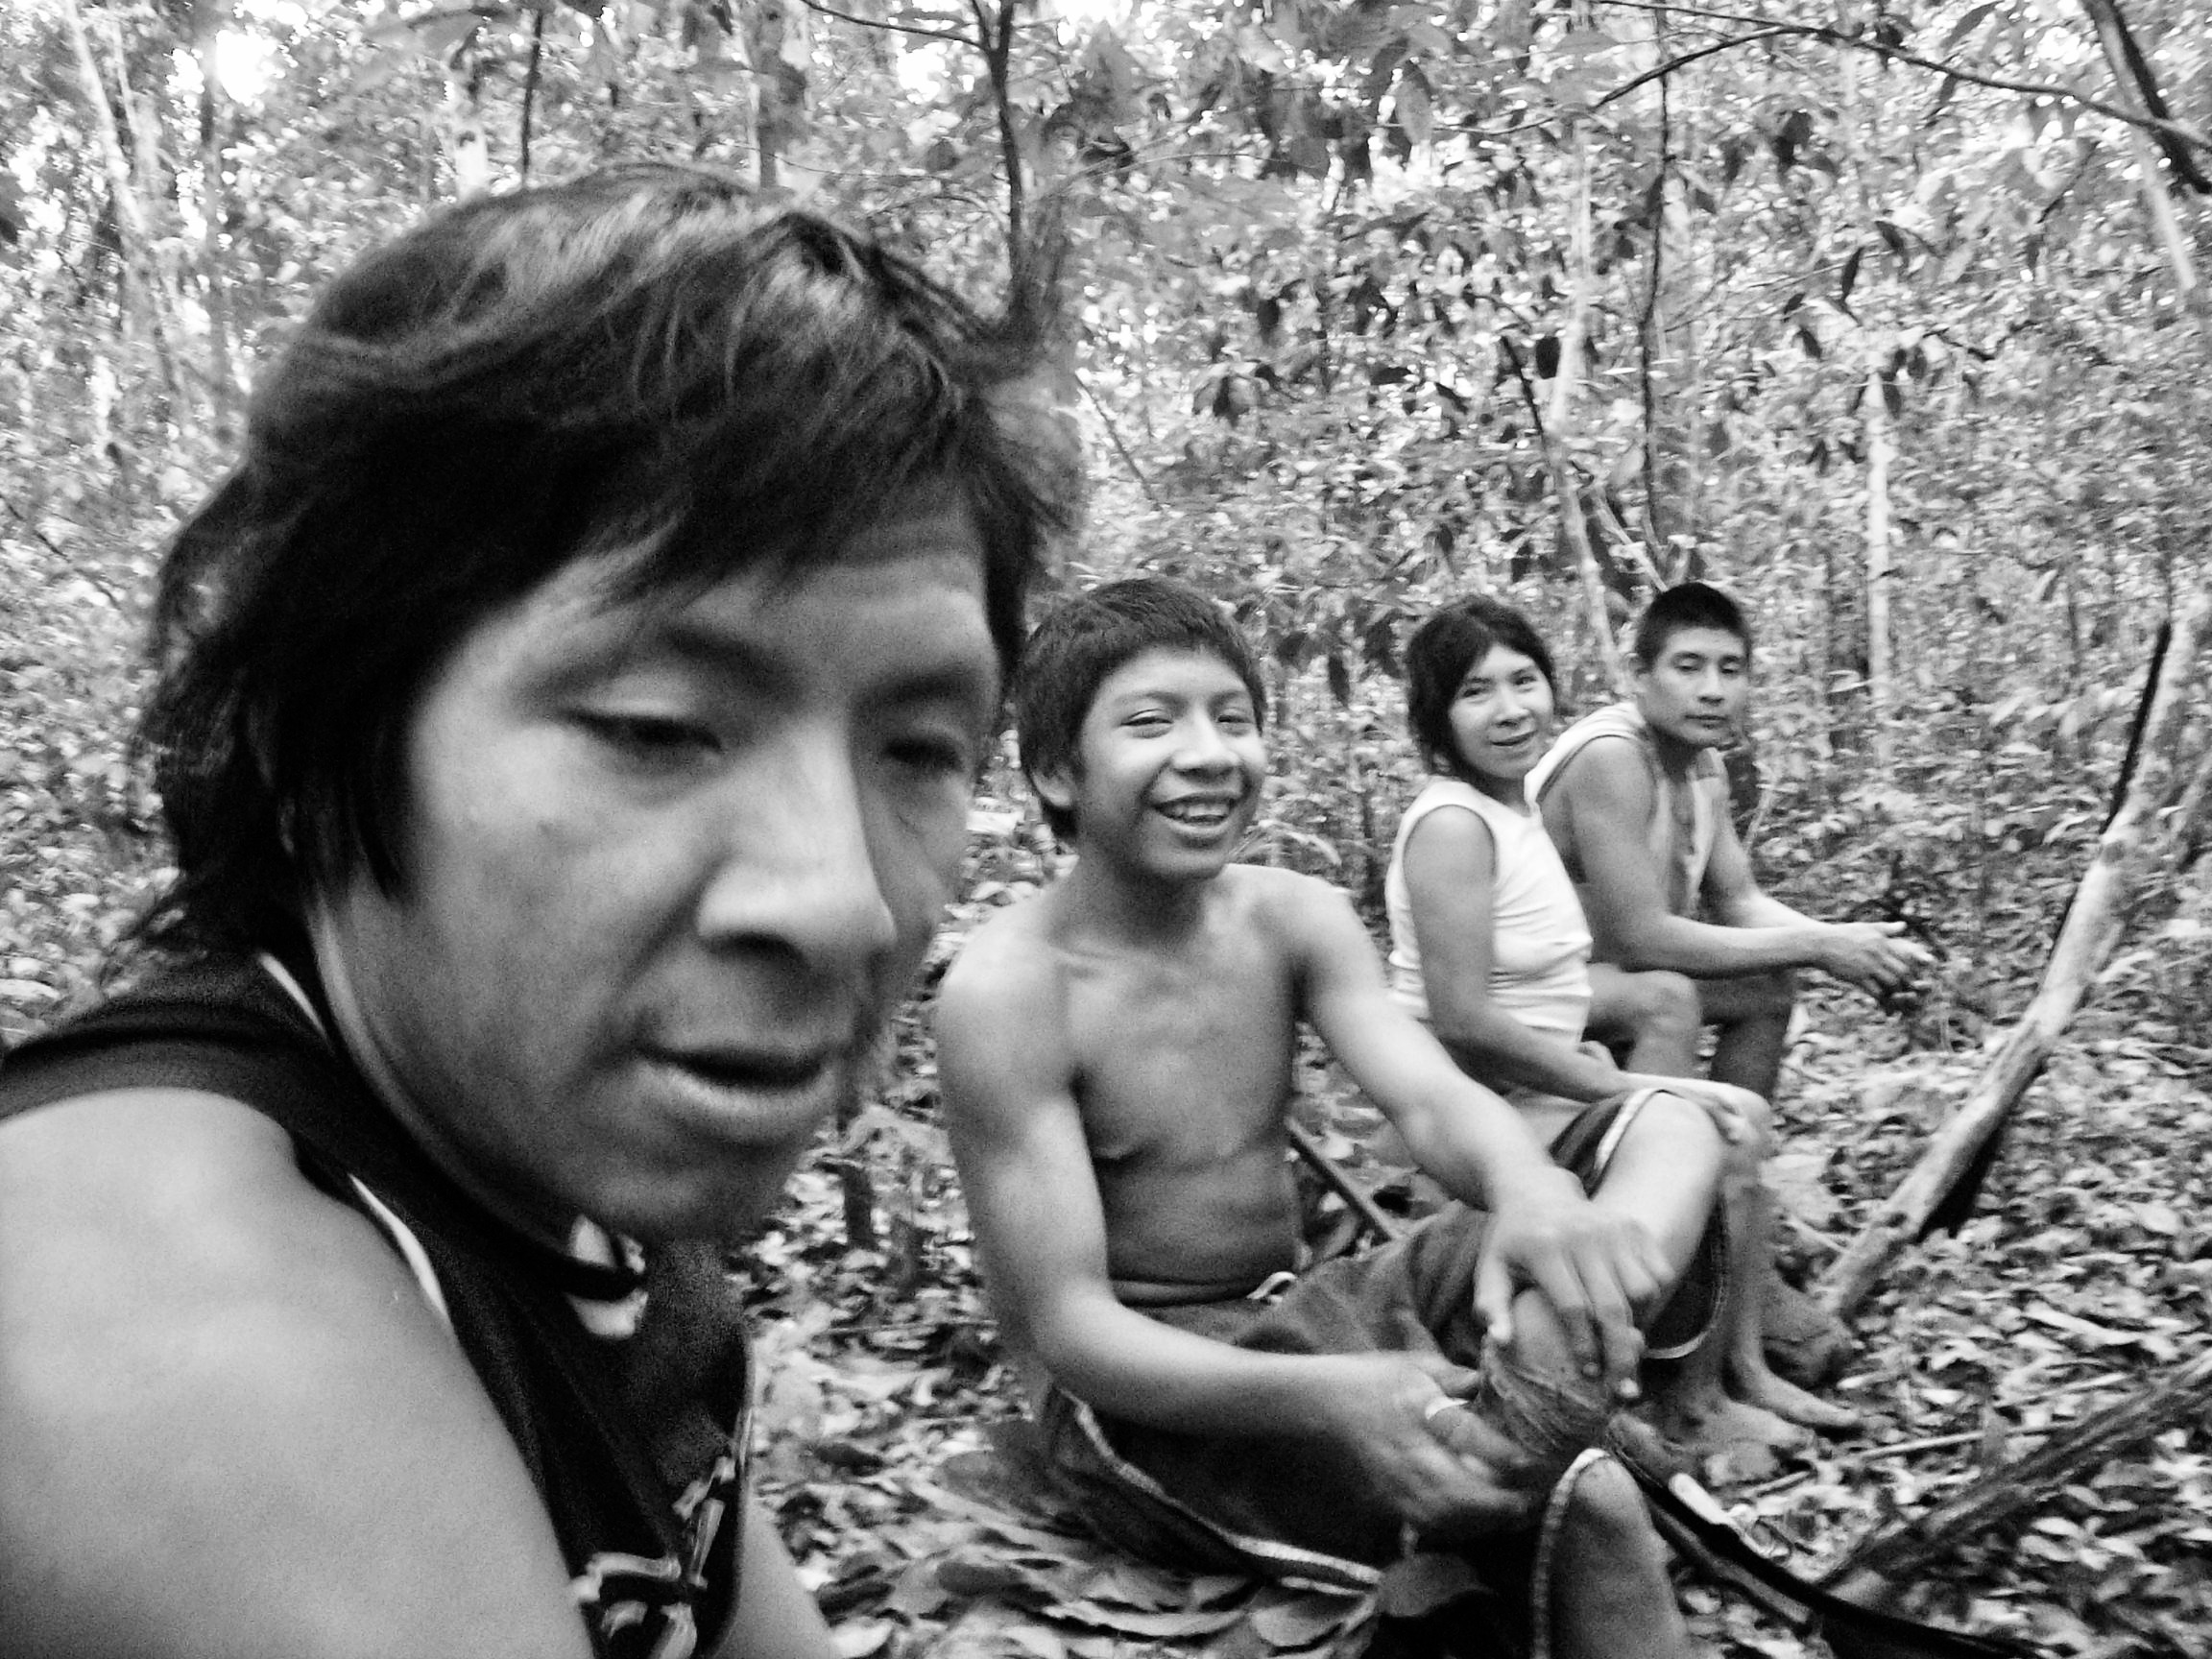
\includegraphics[width=\textwidth]{./imgs/100_5648}
%\caption{Na floresta, descansando durante uma caçada, Uriximatỹa (primeiro plano), Jui’i sorrindo ao lado de sua mãe Ajrua e seu pai Uirahoa (aldeia Juriti, 2007).}
%\end{figure}

\section{distâncias}

\noindent{}As distâncias sociais e genealógicas entre os seres humanos, \textit{awatea}, 
são pensadas mediante as ideias \textit{harapihiara} e
\textit{harapihianã}. \textit{Harapihiara} (\textit{ha}\textit{r-apihiar-a}) é
um termo formado pelo pronome clítico de 1ª pessoa \textit{ha}; o termo
\textit{apihia(r)}, que pode ser traduzido por ``aquele que está próximo''
(como veremos melhor no próximo capítulo); e o sufixo nominal
\textit{a}.\footnote{Trata-se do sufixo nominal \textit{a}, que ocorre com
  raízes nominais tornando-as capazes de exprimir nomes com referência.
  Sem esse sufixo, os nomes funcionam como predicado (p.\,ex. \textit{hamymy} ``eu tenho filho(a)'', enquanto \textit{hamymyra} ``o meu
  filho(a)'') ou como vocativo --- \textit{hamymy, aju kurupi!}, ``meu filho,
  venha cá!'' (Magalhães, comunicação pessoal). O sufixo nominal
  \textit{a} é muito produtivo na língua guajá em palavras como
  \textit{tatu-a}, ``o tatu'', \textit{kwaxi-a}, ``o quati'', e \textit{kwarahy-a}, ``o
  sol'', e pode ocasionar a recuperação de uma consoante final oculta na
  raiz do nome, \textit{r ou -}n, como em \textit{karawar-a}, ``o
  \textit{karawara}'', \textit{harapihiar-a}, como vimos acima, ou
  \textit{amỹn-a}, ``a chuva''.} Já no termo \textit{harapihianã}
(\textit{ha-r-apihia-nã}), o sufixo \textit{nã} denota inautenticidade,
``falso'', fazendo com que \textit{harapihianã} seja algo traduzido como
um ``falso próximo''. E por meio desta pequena diferença os Guajá
distinguem ``consanguíneos e afins `próximos/\,reais' daqueles
`distante-classificatórios'" (Viveiros de Castro, 2002a, p.\,130). Esses
termos ganham, de forma geral, uma ampla acepção. \textit{Harapihiara}
pode ser, por exemplo, os tubérculos que crescem juntos em uma mesma
raiz. Ou as frutas de uma mesma árvore são concebidas como \textit{irmãs}.
E por \textit{harapihianã} podem ser tratados animais com morfologia
parecida, segundo os Guajá.\footnote{O assunto será tratado com mais detalhes no capítulo 6.} Trata-se
portanto de termos de relação para os mundos humanos, animais e
vegetais, e não categorias estritas ao ``sistema de parentesco''. Para
os humanos, \textit{awa}, as pessoas de sua aldeia e as ligadas a
parentes destas podem ser \textit{harapihiara}, ``próximos'', ou
\textit{harapihianã}, ``distantes''; da mesma forma, seres não humanos que
incorporam a suas relações, sejam animais de criação ou os
\textit{karawara} celestes, também são tidos como \textit{harapihiara} ou
\textit{harapihianã}, a depender da proximidade. E diferentes seres no
mundo, para além dos humanos, mantêm entre si relações do tipo
\textit{harapihiara} ou \textit{harapihianã}.

Como ideias de relação, e não recursos vocativos, os termos
\textit{harapihiara} e \textit{harapihianã} organizam o universo dos
parentes, dividindo-o em duas categorias básicas, ``os próximos'' e os
``distantes'', que, em conjunto, formam a humanidade como um todo,
\textit{awatea}, ``gente de verdade''. Desta forma, a definição baseada na
macro oposição ``afins'', ``consanguíneos'' não colabora para o entendimento
destas duas categorias, pois o sistema de aliança guajá, como veremos,
embora também gravite em torno dessas duas ideias, permite que ambas
possam indicar ora ``afinidade'', ora ``consanguinidade'', uma vez que ``a
distinção entre o próximo e o distante é característica de socialidades
em que a residência predomina sobre a descendência, a contiguidade
espacial, sobre a continuidade temporal'', como é o caso em questão.\footnote{Ver
Viveiros de Castro, 2002, p.\,130).}

Doravante, ao discutir as ideias de \textit{harapihiara} e
\textit{harapihianã}, farei referências a distinções variadas (e
complementares), tais como as que vimos acima, devido ao caráter
polissêmico dessas duas categorias, que ora remetem a um código
espacial, ora temporal, e ora diametral, concêntrico. No entanto, a ideia
que conduz minha análise se baseia, fundamentalmente, nas ideias de
``proximidade'' e ``distância'' --- genealógica, espacial e cognática --- tal
como define Viveiros de Castro (1993 e 2002). No caso específico Guajá,
o que distingue essas duas categorias é o sufixo \textit{nã,} que denota
inautenticidade e pode ser encontrado na formação de outros termos
referentes de parentesco, como:

\begin{itemize}
\item\textsc{f}: \textit{tu}\,\,\rightarrow\,\, \textsc{fb}: \textit{tu-nã}
\item\textsc{m}: \textit{ihí}\,\,\rightarrow\,\, \textsc{mz}: \textit{ihi-nã}
\end{itemize}

Assim, ambos os sexos reconhecem o pai (\textsc{f}) como \textit{tu} e o irmão do
pai (\textsc{fb}) como \textit{tu-nã}; e uma vez, ao lhes perguntar sobre tal
classificação, me disseram que a tradução de \textit{tuna} seria ``pai
pouco'' ou ``pai fraco''. O mesmo ocorre para a irmã classificatória de um
homem. Enquanto irmã é referida por \textit{hajnawãi}, uma mulher que seja
tida como irmã de um homem (por ele ter casado com sua filha, por
exemplo) é chamada \textit{hajnawajnã}. Tais soluções podem ser vistas em
outros casos amazônicos, como entre os Waimiri-Atroari, em que parentes
colaterais (\textsc{fb} e \textsc{mz}) ganham o tecnônimo \textit{kî} marcando essa
diferença, assim \textsc{f} é igual a \textit{yimî} e \textsc{fb} é igual a \textit{yimkî}. Trata-se aqui ``do
reconhecimento, no plano terminológico, de dois \textit{graus de distância
lateral} entre parentes consaguíneos, a oposição
linearidade/\,colateralidade é colocada como um epifenômeno da oposição
`proximidade/\,distância'".\footnote{Silva, \textit{op.\,cit.}, p.\,47.} Tudo se passa como se
houvesse uma projeção do sistema perto/\,longe que rege essas relações em
todos os níveis de relação chegando até mesmo à consanguinidade. A
partir dessa ideia e enfatizando o gradiente de proximidade/\,distância
que sobredetermina os termos \textit{harapihiara} e \textit{harapihianã}, como veremos neste e nos próximos capítulos, podemos traduzi-los tanto
por ``próximos/\,distantes''; ``lineares/\,colaterais''; ``cognatos/\,aliados'';
``consanguíneos/\,afins''; ``corresidentes/\,não corresidentes''; e, como parece
confirmar a língua guajá, ``verdadeiros/\,falsos (classificatórios)''. Por
isso minhas definições oscilarão a partir destas múltiplas ideias que
compõem essa complexa oposição, \textit{harapihiara}/\,\textit{harapihianã},
e os exemplos e casos que trarei neste e nos próximos capítulos
determinarão o código a que me estarei referindo. Além disso, podemos
pensar os termos \textit{harapihiara} e \textit{harapihianã} como
macrocategorias, uma vez que eles fazem referência a conjuntos muito
diferentes de relações que vão desde as de parentesco, propriamente, até
a relação entre um animal de criação e seu dono; duplos celestes e
terrestres; partes de um vegetal; um nome e o ser nominado, dentre
outras situações que envolvem seres humanos e não humanos de diferentes
ordens.

Não pretendo discutir aqui o sistema de parentesco (tema do próximo
capítulo), mas, sim, uma terminologia de relações que extrapola o campo
do parentesco e constitui um idioma que informa diferenças e
semelhanças; identidades e diferenças; \textit{harapihiara} e
\textit{harapihianã}.

\section{proximidades}

\textit{Harapihiara} é o termo mais próximo à ideia de um ``nós
cognático'',\footnote{Para essa ideia, ver Albert (1992).} do tipo
``parentes verdadeiros'', cujo casamento é proibido, enquanto
\textit{harapihianã}, além de abranger a classe das pessoas próximas,
porém passíveis de se casar (esposas, maridos, cunhados, sogras, genros
e assim por diante), abrange outras pessoas, \textit{awa}, ``amigas'', \textit{hary} ou \textit{aty}, e ``desconhecidos'' que, uma vez incorporados
via casamento e/\,ou corresidência a um grupo local, podem ser
potencialmente \textit{harapihianã}, tal como encontramos em diversos
casos amazônicos. Para um homem, os \textit{harapihiara} mais próximos de
sua geração são seu irmão (\textsc{b}) e seu primo paralelo paterno (\textsc{fbs}). Para
uma mulher, seria sua irmã (\textsc{z}) e suas primas paralelas bilaterais (\textsc{mzd}/\,\textsc{fbd}). Por isso, o termo utilizado por ego masculino para \textsc{b}/\,\textsc{fbs} e por ego
feminino para \textsc{z}/\,\textsc{mzd}/\,\textsc{fbd} é \textit{harapihiara}, obedecendo-se a
equivalência dos sexos.

A totalidade dos termos de parentesco Guajá,
%(como veremos no próximo capítulo)
tanto para ``afinidade'' quanto para ``consanguinidade'', se
encaixa em alguma destas duas ideias, \textit{harapihiara} e
\textit{harapihianã}, assim como qualquer relação entre seres humanos, \textit{awa}, 
é regida por um ou outro desses termos. Como sabemos, o
componente genealógico e/\,ou socioespacial é parte constituinte do
dravidianato amazônico, atuando como vetor nessas relações e fundamental
à compreensão desses sistemas.\footnote{Ver Viveiros de Castro, 2002, p.\,121;
Silva, 1995; Taylor, 1996; Gow, 1991).} Desta forma, para o caso em
questão, os termos \textit{harapihiara} e \textit{harapihianã}, funcionam
para exprimir as ideias de parentes ``próximos'' ou ``verdadeiros'', \textit{harapihiara}, 
e ``distantes'' ou ``classificatórios'', \textit{harapihianã}. E, apesar do fato de se referirem a diferentes
relações, o conteúdo dessas não está relacionado à sorte automática --- e
binária --- refletida na oposição ``afins'', ``consanguíneos''. Assim, no caso
Guajá, alguns indivíduos que são \textit{harapihiara} entre si podem sê-lo
por laços de aliança ou amizade, ocorrendo, inclusive, em relações entre
indivíduos do sexo oposto, como veremos no caso abaixo.

Em todos os anos de fuga que viveram os Guajá, quando evitavam o contato
e adotavam estratégias de viver entre si, essas ideias estavam operando;
ao serem transferidos para uma aldeia após os contatos, diversas pessoas
que não se conheciam anteriormente passaram a se reconhecer como
parentes próximos ou distantes, e assim as vidas nas aldeias foram
recomeçadas. Panaxĩa e Pira'ima'ã viviam em grupos locais distantes
entre si até a época do contato entre a Funai e o grupo de Panaxĩa, em
1996, quando se juntaram às outras famílias que já viviam na aldeia
Juriti. Pira'ima'ã se casou com a filha de Panaxĩa, Pakwa'ĩa, e desde
então os dois passaram a se classificar como germanos de sexo oposto.

% Verificar tabela
% \begin{figure}[t]
% \centering
%   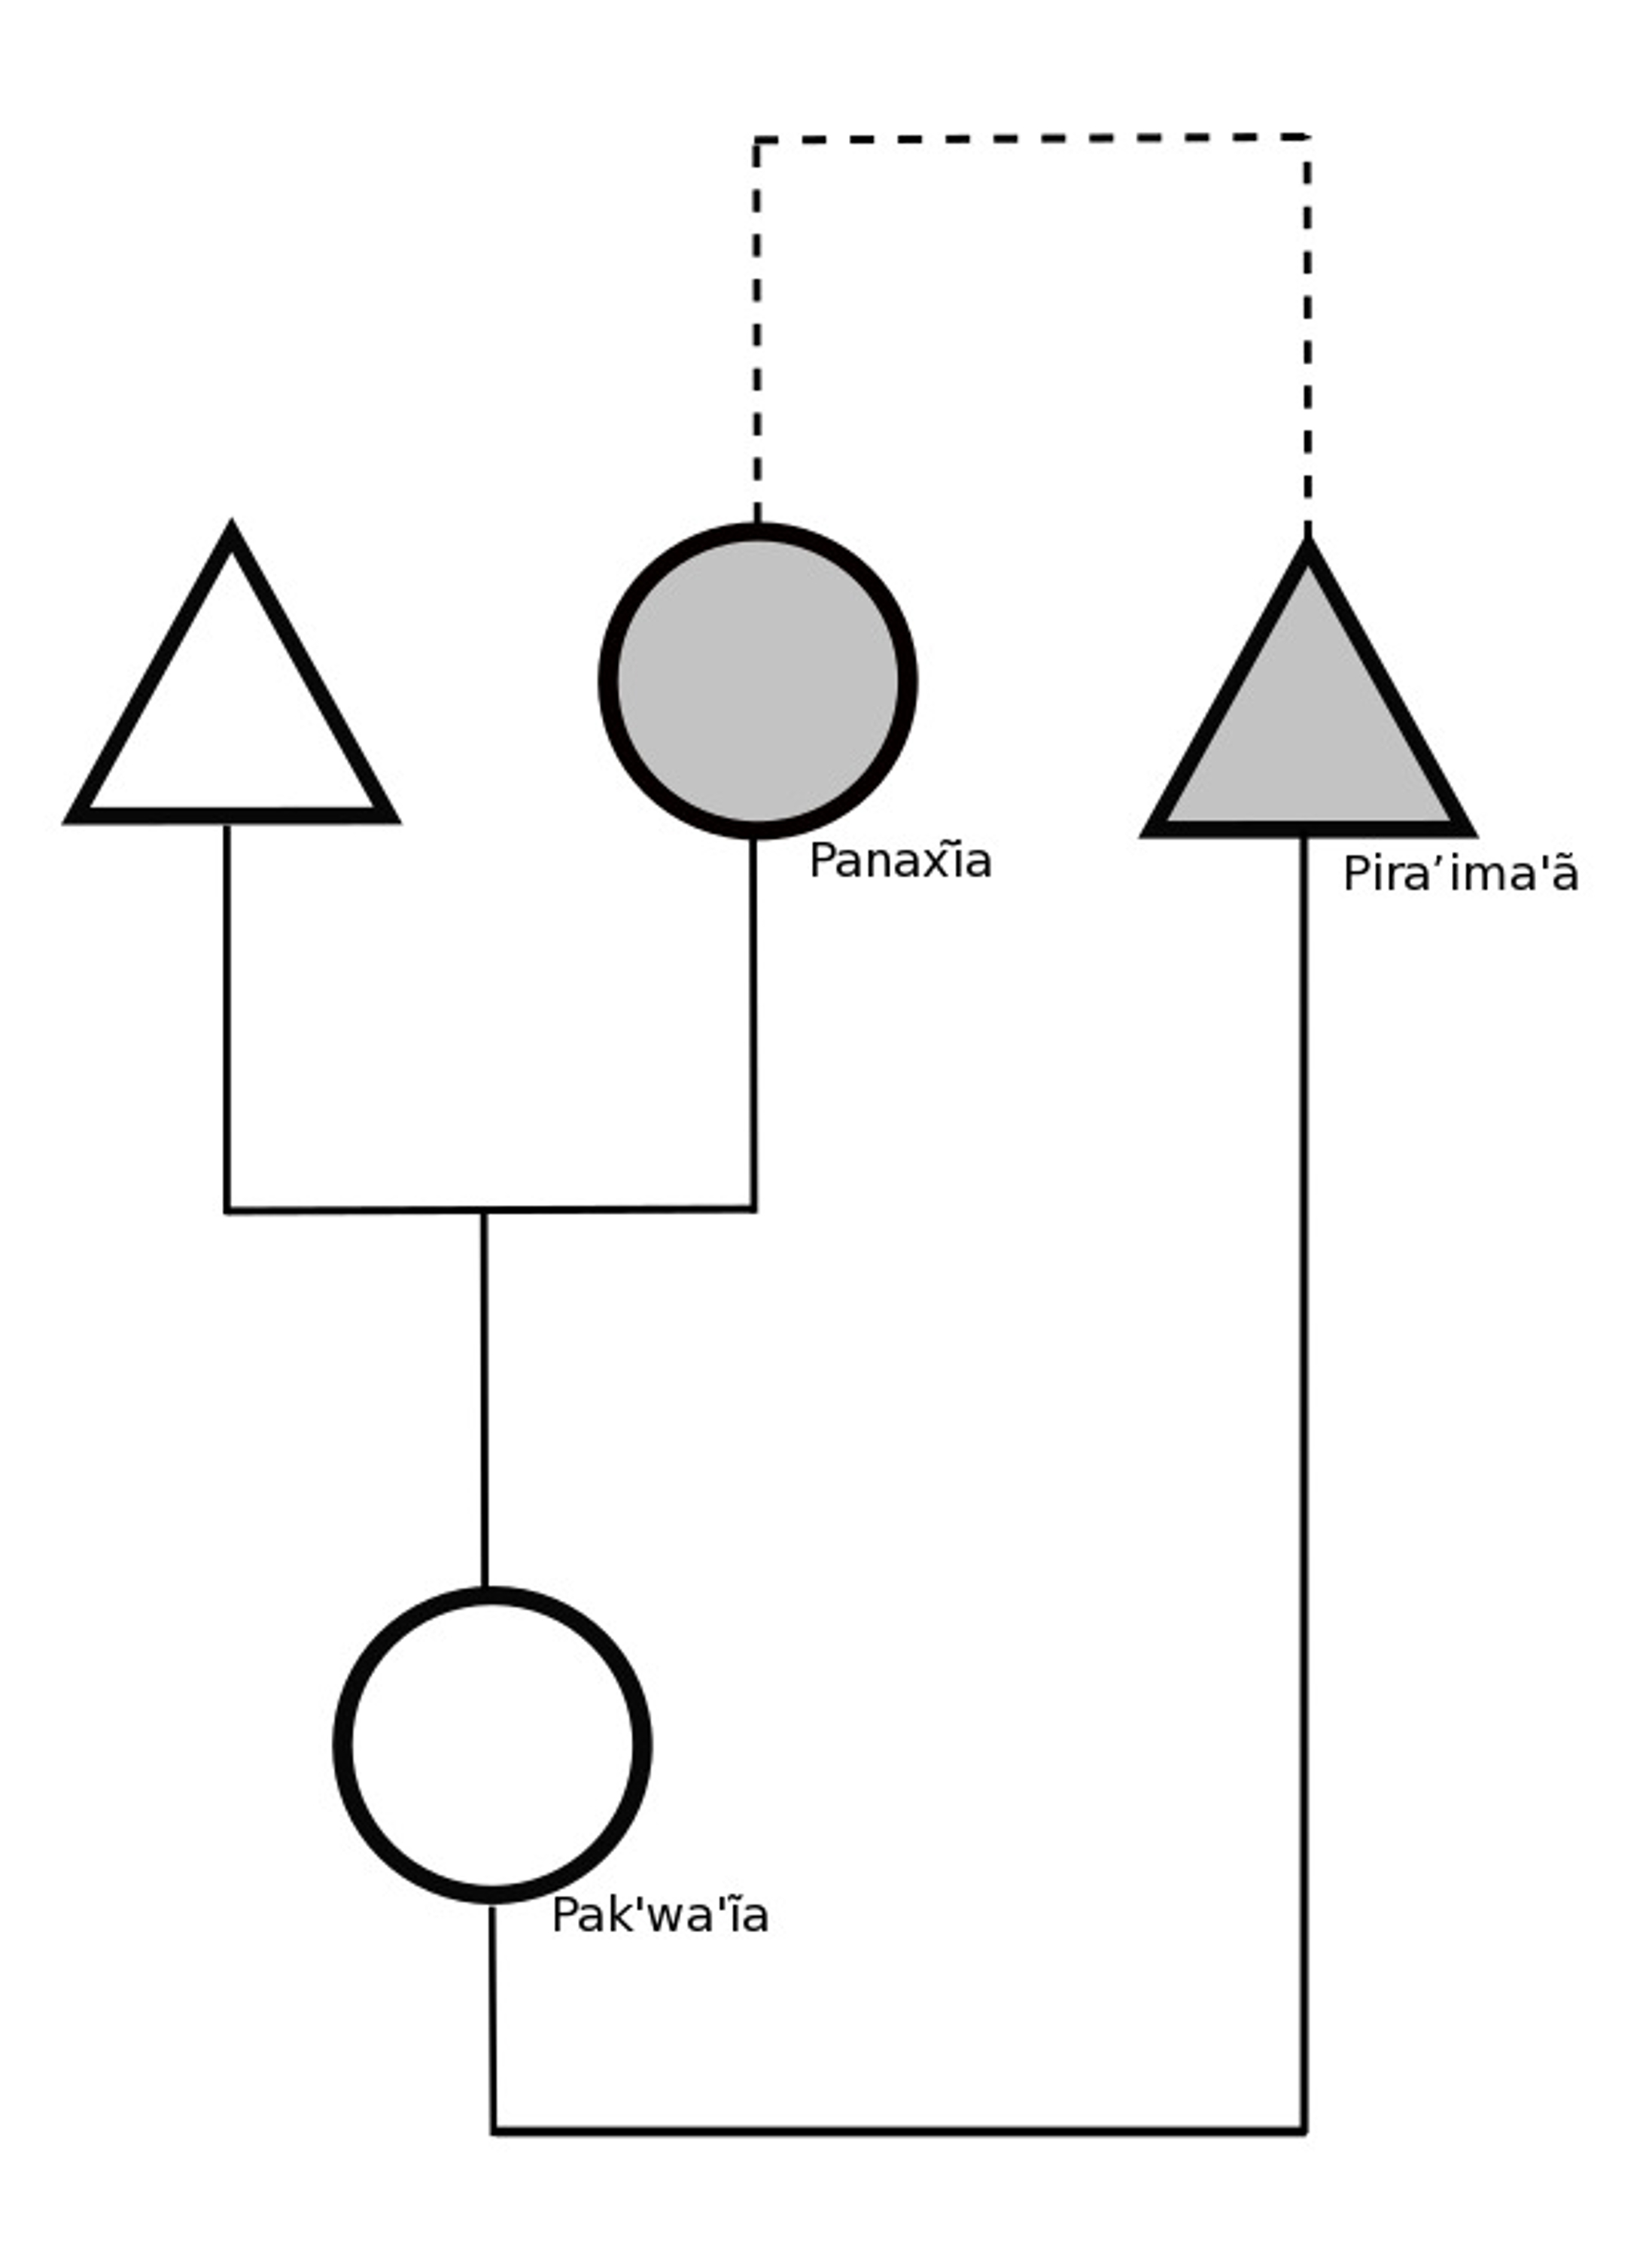
\includegraphics[width=.5\textwidth]{./imgs/Figura_5_crop}
% %\caption{Figura 5}
% \end{figure}

Discutirei essa característica do sistema de aliança Guajá no próximo
capítulo, porém gostaria de, por ora, frisar que dois indivíduos, até
então separados pela genealogia e pela distância física, passaram a
estabelecer entre si uma relação de proximidade, condensada na ideia de
\textit{harapihiara}, quando, antes de uma sucessão de eventos, eram
considerados ``distantes'', \textit{harapihianã}. Tal mudança na forma de
relação é recorrente entre os Guajá e, longe de representar uma
indeterminação dos termos que se alternam em circunstâncias diferentes,
demonstra que as diferenças entre pessoas ``casáveis'' e
``não casáveis'' ou ``parentes próximos'' e ``distantes'' não estão
presas a categorizações fixas --- ``o que impede que se pense a pragmática
social em termos de uma subordinação simples à sintaxe terminológica''.\footnote{Viveiros de Castro, \textit{op.\,cit.}} Se o gradiente de distância é
fundamental para as classificações do parentesco na Amazônia, para um
povo como os Guajá, dentre tantos outros, esta pode ser encurtada ou
estendida ao sabor do tempo e/\,ou da memória, modificando as relações
atuais. Em poucas palavras, um \textit{harapihianã} pode se tornar um
\textit{harapihiara}, e --- com menos frequência --- vice-versa. Todas as
relações entre humanos, \textit{awa}, e toda a humanidade --- ela mesma ---
estão pautados por essa oposição.

\section{das formas de existência}

Vivendo isolados, distantes uns dos outros, desde antes do contato até
os dias atuais, os diferentes grupos locais não formam um ``conjunto
homogêneo Guajá'', tal como prescreve uma idealização de ``grupo
indígena'', com intercâmbios intercomunitários, autoidentificação com o
``grupo'' e alianças em diferentes situações. A forma pela qual os Guajá
sempre se organizaram, sem grandes aldeias ou assentamentos, é reflexo
de socialidade particular, que privilegia formas independentes e
``fragmentárias'' de organização social, marcadas inclusive pelo
estranhamento entre esses pequenos coletivos. Mesmo nos dias atuais, em
que diferentes famílias foram reunidas em uma mesma aldeia, as próprias
aldeias são separadas em setores baseados em grupos de homens
importantes --- \textit{tamỹ}, ``chefes'' --- e, após décadas, repartidos em
quatro aldeias, as pessoas estão se dividindo continuamente em novas
aldeias --- três novas apareceram nos últimos anos, totalizando sete, e não
sabemos quantas ainda virão.

Por exemplo, Ajrua e Juriximatỹa, na década de 1980, antes do contato,
viviam junto com o grupo de Amỹ Pirawãja, mãe de diversos homens
importantes da \textsc{ti} Caru, mas os anos de fuga os separaram e, postos em
aldeias distantes uma das outras, estão há mais de duas décadas sem se
ver, embora, genealogicamente, se acreditem \textit{harapihianã},
``parentes próximos''. Próximos no passado, distantes no presente, o grupo
da aldeia Juriti se refere às pessoas das outras aldeias como de ``boca
diferente'' --- \textit{amõa} \textit{irua}, ou de um ``falar ruim'', \textit{i' ĩ}
\textit{manyhỹ} ---, devido às mínimas variações dialetais encontradas em
cada uma dessas aldeias. Antes do contato, partindo-se de qualquer
\textit{haripa}, ``minha casa-aldeia-acampamento'', os \textit{harakwaha}
mais distantes eram totalmente desconhecidos, assim como os grupos que
neles habitavam. Embora guardem uma história social comum, com dramas e
episódios bastante parecidos, as pessoas de cada região experimentaram
vidas e fugas diferentes, uma vez que sempre viveram afastados uns dos
outros.

No passado, os grupos sem contato evitaram ao máximo o encontro com os
\textit{karaia}, não indígenas, e mesmo havendo outros Guajá contatados
incorporados às frentes de atração, nem sempre isso resultava no sucesso
dessas frentes. Os que estavam na mata desconfiavam da condição de
humanos verdadeiros, \textit{awatea}, dos contatados, já que um dos medos
dos ``isolados'', chamados \textit{mihua}, além das doenças, era perderem
suas mulheres para esses \textit{awa} ``amigos dos \textit{karaia}'', \textit{karai rapihianã}, 
que podiam tanto ser ``parentes'', \textit{awatea}, quanto inimigos --- \textit{mihuatea}, ``desconhecidos''. 
O temor dos ``isolados'' de perder suas esposas está longe de ser infundado,
tendo-se em vista que um dos principais interesses dos homens Guajá que
participam das frentes de atração, até hoje, é a possibilidade de
conseguir novas esposas. Quando da criação do \textsc{pin} Juriti, em 1989, além
do intérprete To'oa que ajudou no contato, outros homens da aldeia
Awá, como Kamajrua, foram lá viver. To'oa casou-se com Amỹ Pirahỹ, que
fazia parte do pessoal recém-contatado, fixou residência na nova aldeia
e passou a exercer certa liderança entre o grupo recém-contatado ---
principalmente nos assuntos referentes à relação com a Funai, o trabalho
na roça, etc. Além disso, outro homem, Takamỹ, que vive na aldeia
Awá, tomou como esposa uma outra jovem desse grupo e voltou a
viver em sua aldeia original, sem nunca mais voltar à Juriti.\footnote{Dada
  a complexidade envolvida em um esquema de viagem intercomunitária, os
  Guajá da aldeia Juriti quase nunca saem para visitar outras aldeias,
  mesmo que tenham parentes vivendo nelas. Uma vez que não existem
  acessos às outras aldeias por dentro do território, qualquer viagem
  entre a aldeia Juriti e as do Pindaré implica sair da jurisdição das
  Terras Indígenas por transportes oficiais (Funai ou Funasa), dormir em
  cidades (na casa de algum funcionário ou hotel), ter gastos com
  alimentação e (muitas vezes) roupas, dentre outras providências que os
  Guajá, sozinhos, não têm meios de viabilizar.}

Ontem e hoje as diferenças continuam marcadas pelos tipos de relação que
cada um dos grupos das diferentes aldeias estabelece. Como já mencionei,
a maior parte de minha pesquisa de campo foi desenvolvida na aldeia do
\textsc{pin} Juriti, uma comunidade pequena que em 2013 contava com 66 pessoas.
Como escrevi anteriormente, quase tudo o que aprendi com os Guajá se deu
entre essas pessoas, inclusive suas ideias sobre os outros grupos
humanos que viviam em outras comunidades e que com eles tinham
pouquíssimo contato, a não ser quando iam, quase sempre por motivos
médicos, para Santa Inês ou mesmo para São Luís. Em diversas situações
me lembravam como eles são diferentes dos Guajá das aldeias de Tiracambu e Awá, 
e, sem mencionar os moradores da aldeia do \textsc{pin}
Guajá (aldeia do Cocal), caso extremo de estranhamento para os Guajá do
Juriti, me diziam estarem ``doidos'', \textit{wakyhy}, por beber cachaça e
fumar cigarro, tal como fazem os Tenetehara e os Ka'apor.\footnote{Por
  não usarem tabaco, os Guajá falavam mal dos Tenetehara e os Ka'apor
  por fazê-lo. Além disso, diziam-me que não fumavam porque lhes faria
  muito mal.}

As pessoas da aldeia Juriti maldiziam as das aldeias Awá e Tiracambu por
terem feito alianças com os Guajajara (Tenetehara), uma vez que sempre
mantiveram com os Tenetehara uma relação de desconfiança, devido a
conflitos passados. Em diversas ocasiões sugeriram que eu ``desistisse''
de realizar meu trabalho de campo junto aos Guajá do Pindaré (aldeias
Awá e Tiracambu), uma vez que os de lá, por estarem ``misturados'', 
\textit{iku} \textit{pamẽ}, com os Guajajara, também estariam bebendo e
fumando muito. No entanto, quando cheguei à aldeia Tiracambu, as pessoas
de lá me pediam justamente para que eu não retornasse à aldeia Juriti,
pois, devido a seu relativo isolamento, era um lugar desconfortável e
difícil de chegar. Falavam também que meus amigos da aldeia Juriti
seriam ``gente do mato'', \textit{awa} \textit{ka'apahara}, ou mesmo
\textit{awatea}, ``gente de verdade'', que nesse sentido era sinônimo de um
tipo de existência --- no qual se vivia nu, dormindo em tapiris, sem
agricultura e fugindo --- que as outras aldeias não querem mais
experimentar.

O resultado dessa diferenciação é que tais ``parentes'', entre si, seriam
\textit{amõ awa}, ``outros Guajá''. Devido às diferenças
político-geográficas desde a aldeia Juriti, todo tipo de críticas aos
Guajá do Pindaré, das aldeias Awá e Tiracambu, me foram relatadas --- a fim de
me dissuadir de uma possível aproximação com as outras aldeias ---, e a
principal delas é que as pessoas alardeariam minha presença para os
Guajajara, com o intuito de eles me expulsarem da terra indígena. Para
evitar isso, pediram para que eu não passasse longas temporadas naquelas
aldeias; e, ainda, para que eu tivesse cuidado com minha alimentação,
pois os Awá das outras aldeias comiam animais que eles haviam descartado
de sua dieta, como preguiças, onças e sucuris --- alegando que os Guajá do
Pindaré são dotados de um fígado, \textit{ipia'akera}, diferente do deles,
mais preparado para tolerar tais carnes; dentre outras observações.

Forline\footnote{Comunicação pessoal.} conta que, no ano de 1993, a administração da
Funai resolveu abrir uma trilha por dentro da \textsc{ti} Caru que ligasse a
aldeia do \textsc{pin} Awá à do \textsc{pin} Juriti,\footnote{Nesta época, os Guajá estavam
  sob a administração regional da Funai de Belém, que tomava decisões
  (ainda mais) autoritárias e sem qualquer critério razoável no que
  dizia respeito ao processo de contato e estabelecimento em aldeias dos
  grupos Guajá isolados.} como que para propiciar uma espécie de
``intercâmbio'' entre aldeias tão distantes, incluindo-se matrimônios e
alianças para maior vigilância da área indígena. A viagem, que durou 13
dias por dentro da floresta, partiu da aldeia Juriti em direção à aldeia
do \textsc{pin} Awá, atravessando uma região repleta de morros. Na equipe, além
dos funcionários da Funai, estavam muitos jovens da aldeia Juriti, além
da família de Takwarẽxa'a, contatada no ano anterior. Porém tal
iniciativa só gerou mal-estar entre as aldeias: algumas pessoas estavam
com gripe e tuberculose e acabaram trocando, não mulheres, mas,
doenças. A, então, jovem Pikawãja, irmã de Wirahoa, foi pega
--- \textit{pyhy}, ``tomar'' --- em casamento por Takamỹ, da aldeia do \textsc{pin} Awá.
Algumas pessoas do \textsc{pin} Awá ameaçaram de morte os Guajá do \textsc{pin} Juriti,
pois não gostaram que muitos deles se enamoraram por mulheres de lá,
dentre outros entreveros. Nesse ínterim, o coordenador da expedição,
Fiorello Parisi, percebeu que sua ideia não havia sido bem-sucedida e
foi embora, deixando para trás um quadro de animosidade para eles
resolverem entre si. O resultado foi que as pessoas da aldeia Juriti
usaram o mesmo caminho de ida para voltar a sua aldeia; perderam uma
mulher e ainda foram ameaçados de morte.

Durante os meus períodos de campo na aldeia Juriti, eu tinha por missão
informá-los sobre como estão --- ou melhor, são --- as pessoas da aldeia
Tiracambu; e o inverso também ocorria. O principal interesse do grupo da
aldeia Tiracambu era minha experiência entre os Guajá da aldeia Juriti.
Ambos me questionavam: se os outros tinham bastante caça; como eram suas
roças; como eram as estruturas da Funai; se havia mulheres; como eram
as crianças; se eram nervosos, \textit{imahy}, ou calmos --- \textit{katy},
``bons'' ---; dentre outras inúmeras indagações. As diferenças entre esses
grupos Guajá variam em atitudes, dieta, e chegam a pequenas diferenças
na fala que, muitas vezes, os Guajá da aldeia Juriti diziam ser
imensuráveis. Vejamos algumas.

\section{comida}

\textit{Awa nimi'ũa}, ``comida de gente'', entendida por carnes variadas,
mel, frutos e também farinha, arroz, bolachas, dentre outros, se opõe,
por exemplo, a \textit{karai nimi'ũa}, ``comida dos não indígenas'', repleta
de sal e carnes que os Guajá ``não sabem'' comer da maneira apropriada,
como a carne de gado e frango, pois poderia fazer mal. Ou \textit{awa mihu
nimi'ũa}, ``comida de índio brabo'', se refere à subdieta pela qual
passam os Guajá que vivem em isolamento voluntário, cheia de animais
nocivos, como cobras e ratos, tubérculos, como cará-do-mato, e frutos, 
como a pequirana, que as pessoas da aldeia não toleram hoje em dia ---
esta é uma dieta de ``antigamente'', \textit{imỹna}.

Ao mencionar as diferenças internas à uma comunidade Guajá, Cormier
lembra que o fato de diferentes grupos terem sido trazidos para viver
juntos na reserva Caru fez com que cada um deles trouxesse um padrão
diferente de alimentação, e, embora próximos uns dos outros, eles
diferiam em pequenas coisas. Dessa forma, alguns tinham mais receio de
comer determinados alimentos do que outros (Cormier, \textit{op.\,cit.}, p.\,40).
As diferenças alimentares marcam as distâncias que separaram os grupos
Guajá durante toda a sua história, do passado ao presente. Dos animais
de que os Guajá se alimentam,\footnote{Ver Forline, 1997; ver também Cormier,
2003).} à exceção dos que os humanos nunca comem (como, por exemplo,
corujas, urubus, morcegos, gambás, raposas, coelhos e
esquilos, ou quatipuru), os \textit{awa} são muito tolerantes a sabores,
texturas e eventuais toxidades que um alimento possa carregar; e, por
mais absurdo que possa parecer, é muito difícil fechar uma relação de
animais interditos. Até 2013, eu não sabia do consumo de capivara, \textit{kapijawara}, 
mas Warixa'á, que vive na aldeia Awá, disse que ele
e alguns homens comiam, mas realmente é uma carne ``reimosa'', \textit{manahỹkera}, 
proibida às mulheres, e nem todos os homens a
toleram. Sobre as onças, podia se dizer o mesmo: na aldeia Awá, até as
onças pintadas podiam ser matéria de consumo de alguns coletivos, ao
passo que na aldeia Juriti, mesmo a sussuarana (que todos dizem ter uma
carne saborosa como a do veado) era consumida por poucas pessoas e ainda
com parcimônia. No limite, a dieta reflete algo fundamental de toda a
socialidade \textit{awa} que impossibilitaria fecharmos uma ideia geral de
``sociedade'' ou ``povo'' como um todo homogêneo. Afinal, sabemos ---
desde autores como Marilyn Strathern, em \textit{O gênero da dádiva}, por
exemplo --- que a \textit{Sociedade} seria mais um problema de ``nós'',
antropólogos, do que de nossos interlocutores (Strathern, 1988, p.\,3).

Muitos animais são apreciados por alguns e desprezados por outros, a
depender da aldeia. Após o contato, com a junção de diferentes grupos
locais em um mesmo lugar, a tendência seria que em cada aldeia a dieta
se estabilizasse e que animais antes apreciados fossem descartados por
motivos variados --- que vão desde a pouca quantidade de gordura até a
nocividade de determinada substância ao corpo humano, passando pelo
sabor e consistência. O fato de alguns Guajá comerem o que os de outra
aldeia não comem não passa por uma noção do tipo ``tabu'', mas, como eles
mesmos propõem, uma diferença congênita --- tal como sabemos há algum tempo
a respeito da corporalidade dos povos amazônicos\footnote{Ver Seeger \textit{at
all}, 1979.} que, nesse caso, é expressa pela ideia dos diferentes tipos
de fígado, \textit{ipia'akera}, das pessoas. Quando algumas pessoas da
aldeia Juriti afirmam nunca terem consumido determinados alimentos, não
é possível generalizar o argumento para todos os outros Guajá, nem mesmo
daquela mesma aldeia. Certa feita, ao matarem um tamanduá, \textit{tamanawã}, 
animal cujo sabor era de duvidoso apelo culinário --- e
sempre disseram não gostar, pois afirmam fazer mal, \textit{manahỹ}, além
de ser fedorento, \textit{irymyhỹ}, e reimoso, \textit{manahỹkera}, --- dois
homens mais velhos, além de consumir o tamanduá ofereceram-no a alguns
rapazes para experimentarem. Outros homens adultos me disseram que não
comeriam, pois, desde sua mudança para o posto indígena, não mais se
interessavam por carnes como aquelas consideradas \textit{manahỹ}, ``ruins'', ``feias'', 
e \textit{iramyhỹ}, ``fedorentas''. O mesmo ocorreu com
uma sussuarana, \textit{jawaraporõ}, --- animal que consumiam antes do
contato --- que, depois de abatida, alguns cogitaram transportar para a
aldeia para comê-la, porém foram dissuadidos por outros por acharem que
não valeria a pena, uma vez que estávamos no meio de uma viagem para um
acampamento de caça. Carnes como a de tamanduá-bandeira, \textit{tamanawã}, 
sussuarana, \textit{jawaraporõ}, porco-espinho, \textit{kwanũa}, 
cuandú, ou ouriço-cacheiro --- \textit{Coendou prehensilis}, e
tamanduá-de-colete ou a mambira, \textit{tamãnawã'ía} --- \textit{Tamandua
tetradactyla}, têm suas qualidades de bom alimento, além da segurança da
ingestão, postas à prova e figuram no grupo das pouco apreciadas, por
``fazerem mal''; mas podem ser consumidas por alguns, principalmente
entre os que assim faziam antes do contato.

O quati, \textit{kwaxia}, da mesma forma, tem uma carne bastante
apreciada, principalmente devido a seu potencial gorduroso. Nos meses de
inverno, época da oferta de gordura nos animais --- \textit{ikira ra'o}, ``muito gordo'' ---, 
o quati é consumido por todos, porém alguns cuidados no
manuseio dessa carne devem ser observados. Diferentemente de animais como os macacos, 
dos quais se aproveitam as vísceras, \textit{ha'aikera}, como aperitivo 
(principalmente entre os velhos), o quati deve ser manuseado e limpo, \textit{hape}, 
em separado das outras carnes, dado o ``fedor'', \textit{irymyhỹ}, que exala. Embora para meus
limitados sentidos o cheiro das vísceras do quati não diferisse do de
outros animais do mesmo porte, como os tatus, meus amigos distinguiam
muito bem seu odor, que tem faculdades, cheiros patogênicos, \textit{mixahy}, 
e afeta diretamente a saúde humana. Devido aos possíveis
danos à saúde, quem o limpar deverá cuspir a todo momento para que o
cheiro não penetre na própria carne nem adoeça. Quase sempre o limpam
longe da cozinha, de preferência em uma área do rio destinada a isso,
lavando-o para que fique purificado, sem o odor das vísceras. Só assim
sua carne estará pronta para consumo. Certa ocasião, quando eu estava
com um grupo de pessoas na casa de Wirahoa, Juxa'a voltava do rio em
direção ao moquém com dois quatis já bem limpos. Ao passar por nós,
todos começaram a cuspir com receio de que o odor do animal ainda lhes
viesse a fazer mal. Uma das explicações, como já observei, é o fato de
os quatis, assim como os gambás, estarem relacionados aos espectros
\textit{ajỹ.}

Outros animais que também figuram no grupo de alimentos perigosos são as
galinhas, \textit{xamakaja}. Após o contato, as aldeias ficaram repletas
de galinhas, introduzidas junto com as roças, as novas casas e com tudo
que estava relacionado à nova vida. Toda galinha pertence a alguém,
inclusive muitas crianças são donas, \textit{jara}, de galinhas. Por serem
animais domésticos, \textit{nima}, --- e como animais domésticos não são
abatidos ---, quase nunca eram consumidas.\footnote{Nos últimos anos, sobretudo nas
aldeias Awá e Tiracambu, isso está mudando.} As galinhas da aldeia se
alimentam de restos de alimentos, pequenos insetos e baratas. Para se
ter uma ideia, das primeiras vezes em que estive na aldeia Juriti,
quando a população era de 40 pessoas --- atualmente, 66 ---, contei mais de
50 dessas aves, entre pintos, frangos e galinhas. Naquela época, todas
as vezes que mataram galinhas estavam com pouca ou nenhuma carne há dias
e, ``pressionados'' por algum branco, \textit{karaia}, do posto indígena que
os aconselhava a comer para matar a fome, se aventuravam em abater uma
delas, que era consumida principalmente pelos homens. A carne da galinha, 
\textit{xamakaja}, na aldeia Juriti, até poucos anos atrás, era interdita
para as mulheres --- tal como a carne de veado, discutida no
capítulo anterior --- por ter propriedades nocivas que podem interferir na
menstruação. Porém, hoje em dia as mulheres já a comem, ``mas comem
pouco'', como me disse Pira'ima'ã. E mesmo os homens ao consumi-la o
fazem com desconfiança, já que se trata, ainda que de uma forma torta,
de um animal de criação, um \textit{nima}.\footnote{Para outra abordagem,
  ver Cormier (2003, p.\,97), em que a autora enfatiza que, segundo os
  Guajá, as galinhas seriam \textit{karai nima}.} Já os ovos, \textit{xamakaj rapia'a}, 
eram consumidos por todos, sem maiores
problemas. Bem diferente do que fazem os funcionários do posto, e de
maneira bem eficiente, o abate de uma dessas aves é sempre catastrófico,
uma vez que a possibilidade de simplesmente quebrarem-lhe o pescoço,
darem uma paulada na cabeça ou lhe cortarem a garganta, tal como fazem
os \textit{karaia}, os ``brancos'', está descartada. O abate costuma ser feito
por garotos que querem treinar pontaria, e quase sempre o animal é
espreitado e morto a flechadas. Muitas vezes, pressentindo o ataque, a
galinha foge para a capoeira que circunda a aldeia e lá permanece por
vários dias na tentativa de uma sobrevida. É comum encontrarem-se
galinhas cegas com um olho perfurado ou mancas por terem sido alvejadas
e conseguido escapar que, após alguns dias, voltam para a aldeia sem
terem sido mortas.

O consumo de capivaras, urubus, morcegos, mucuras, ratos, raposas,
coelhos, esquilos, duas espécies de jacu, onça-pintada, \textit{jawaruhua}, 
além da maior parte de espécies de cobras, é
interdito a todos os Guajá;\footnote{Ver Cormier, \textit{op.\,cit.}, pp.\,41--42.} mas, como
já adiantei, pessoas diferentes de comunidades diferentes dizem tolerar
carnes, por exemplo, da capivara ou da onça-pintada, e os ratos, lembram
os Guajá, eram consumidos em espetos antes do contato, bem como a carne
da rã \textit{iwê}. Quanto à jiboia, \textit{majhua}, na aldeia Juriti
alguns consideram seu consumo algo do passado --- do ``tempo da floresta'',
\textit{imỹna} \textit{ka'ape} ---, e nos dias de hoje não são comidas,
enquanto outros consideram ser essa uma boa carne, diferente da carne de
cobra, \textit{inami'ĩa}. A jiboia --- diferente de outras espécies como a
jararaca, cascavel, coral (e falsa-coral), sururucucu ``pico de jaca''
(\textit{Lachesis muta}) --- não é considerada \textit{inami'ĩa}, ``cobra
(venenosa)''.\footnote{A jararaca, inclusive, é denominada
  \textit{inami'ĩtea}, ``legítima cobra venenosa''.} Assim como o capelão, 
  \textit{waria}, não é considerado parte do universo dos ``macacos''
(voltarei a esse ponto nos próximos capítulos), a jiboia não é uma
``cobra'', no sentido comum de \textit{inami'ĩa}, porém, outra espécie
animal --- tal como uma anta, que não possui correlatos com outros
animais. Certamente o consumo de jiboia e de outros animais oscilam ao
sabor da situação e da vontade de variar --- alguns dizem gostar, ao passo
que outros defendem não mais consumir. Quanto à sucuri e à surucucu,
desde o início me explicaram serem animais completamente nocivos --- por
isso nunca consumiam ---, embora houvesse uma família que vivia apartada,
foi realocada na aldeia juriti e comia cobras.

Como hoje em dia cada aldeia tem uma conformação específica, que varia
desde o número de habitantes à oferta de determinadas caças nos
diferentes ambientes, há diferenças na dieta entre elas.\footnote{Por
  exemplo, a oferta de macacos \textit{tapajua}, mão-de-ouro (um pequeno
  macaco do gênero Saimiri --- \textit{Saimiri sciureus}), animais muito
  apreciados para alimentação nas aldeias Awá e Tiracambu,
  é quase inexistente na aldeia Juriti, e por isso não figura em sua
  dieta.} Até mesmo algumas interdições, vistas como comuns --- se assim
posso colocar --- estão sujeitas a novas conformações locais. É o caso dos
frutos da bacaba, \textit{pinawã}, e do açaí --- \textit{jahara}, ``juçara''. Na
aldeia Juriti, o fruto do açaí, \textit{jahara}, era uma interdição para
todos, uma vez que a aparência sanguinolenta do líquido --- \textit{tekwera}, ``caldo'' --- 
extraído seria nocivo a quem o tomasse. Por isso classificam o
caldo do açaí como \textit{jahara rawya}, que pode ser traduzido tanto por
``sangue do açaí'' quanto por ``veneno do açaí'', uma vez que \textit{hawy}
permite essas duas traduções, e ambas se aplicariam aqui. Considerada a
inevitável semelhança entre o sangue e a polpa do açaí, essa é uma forma
de enfatizar a nocividade do alimento. Em uma única situação em que
estive presente, quando conseguiram açúcar junto ao posto indígena,
alguns homens comerem a polpa de açaí, mas me explicaram que nenhuma
mulher poderia fazê-lo sob o risco de afetar (de novo) seu ciclo
menstrual, pois se o açaí tem esse inegável aspecto sanguinolento, \textit{hawy}, 
atuaria no aparelho reprodutivo das mulheres.\footnote{Mesmo
  que este livro careça de informações sobre temas como concepção,
  menstruação e reprodução sexual, posso afirmar que os Guajá não têm
  uma palavra exclusiva para indicar sangue menstrual ou menstruação.
  \textit{Hawy}, ``sangue'', de forma geral, é utilizado quando se referem
  ao sangue menstrual.}

Ao contrário do açaí, a bacaba, \textit{pinawã}, é um dos alimentos mais
apreciados por todos. Além do sabor agradável, a aparência leitosa e
clara é dita benigna para o corpo e, assim como outros alimentos, como o
mel e as gorduras animais, a bacaba ``faz a barriga rir'' --- \textit{hakatohõ}, ``barriga cheia''. 
O contraste dos discursos entre a alva e nutritiva
bacaba e o sanguinolento e nocivo açaí era tão marcado na aldeia Juriti
que imaginei ser generalizado em outras aldeias. Porém, ao passar alguns
dias na aldeia Tiracambu, vim a descobrir que lá o açaí é tão apreciado
quanto a bacaba --- homens e mulheres comem do fruto sem qualquer
constrangimento. Conversando um tempo depois com as pessoas da aldeia
Juriti, eles me disseram simplesmente (o que sempre dizem em casos como
esses): que as pessoas da aldeia Tiracambu ``sabem'' --- \textit{kwa}, ``eles
sabem'' --- comer o açaí, enquanto eles ``não sabem'', \textit{nikwaj}. Nos
últimos anos, depois de os homens da aldeia Juriti começarem a consumir
açaí, as mulheres também o fazem.

Como já mencionado, as escolhas alimentares dos diferentes grupos locais
foram moldadas pela história e regiões em que viveram. Questão crucial a
respeito de povos como os Guajá --- cujo contato com o Estado é muito
recente ---, as características de sua dieta podem, de uma forma geral,
ser pensadas por antes e depois do contato com os
\textit{karaia}.\footnote{Ver o caso dos Parakanã ocidentais, em muitos
  aspectos semelhante ao dos Guajá (Fausto, 2000, pp.\,156--157).} Tamanduás,
onças, cobras, cuandus, ou ouriços, além de algumas espécies vegetais como a
pequirana, \textit{myky'arỹ}, foram rapidamente retirados da dieta (ou
seu consumo foi drasticamente reduzido) após o contato, por não serem
artigos tão apreciados. Vários fatores o influenciaram: (1) a reunião de
grupos distintos com hábitos alimentares ligeiramente diversos engendrou
uma padronização ótima da dieta; (2) o baixo apreço por determinadas
carnes que, confrontadas com a oferta de novos gêneros alimentícios
trazidos pela introdução da agricultura, foram deixadas de lado sem
muito pesar; (3) incomensuráveis mudanças pós-contato que passam (além
da dieta) por habitação, relações conjugais, proximidade com o mundo dos
brancos, que alteraram radicalmente a possibilidade de manter a ênfase
em antigos alimentos, como diversas espécies de mel e larvas; dentre
outros fatores. Talvez a principal alteração na dieta pós-contato possa
ser observada pelo aumento no consumo de peixes, consequente à
introdução de anzóis, linhas e tarrafas como instrumentos de pesca. Se
os Guajá, até antes do contato, eram caçadores especializados em
determinados tipos de mamíferos terrestres de grande porte --- como
ungulados (queixada, caititu e anta) e dois tipos de cervídeos junto com
roedores (anta e paca), além de possuírem uma apurada técnica de caça
para primatas e outros mamíferos arborícolas, como capelães,
macacos-prego, além de quatis ---, o consumo de peixe, por sua vez, não
era representativo em sua dieta de proteína. Porém, devido à introdução
dos instrumentos de pesca, os peixes são um importante complemento da
alimentação nos dias atuais, sobretudo nos meses de verão. Devo
ressaltar que, com exceção de alguns surubins, \textit{iriwia}, trata-se
de peixes (devido ao baixo potencial piscoso do rio Caru) pequenos e
médios, como sardinhas, \textit{pirapopoa}, pequenos bagres, ou mandis, \textit{hirakatỹa}, 
mandi-sacaca, \textit{hirakatorohõ}, diversos tipos
de piaus, \textit{hipia}, piranhas, \textit{ipinẽa}, curimatá, \textit{piraxĩa}, 
dentre outros menos pescados.

Comer o animal correto também é fundamental para a boa formação de um
corpo, e para as pessoas, \textit{awatea}, existe uma relação direta entre
o porte do animal ingerido e as qualidades alimentares de sua carne,
como se fossem diretamente proporcionais. Trocando em miúdos: o
crescimento de uma criança será mais bem-sucedido se ela comer animais
de grande porte. Com a pequena esposa ocorre exatamente o mesmo, tanto
mais bela, \textit{parahỹ}, crescida, \textit{ixa'a}, e saudável, \textit{katy}, 
ela será quanto mais carnes grandes --- e, por isso,
saudáveis --- ela ingerir. Se uma pessoa for criada durante a infância
comendo apenas pequenos peixes (piabas, pequenos mandis, sardinhas,
pequenas piranhas, muito comuns no rio Caru) e animais de pequeno porte
como cotias e quatis, isso comprometerá seu crescimento. Os Guajá da
aldeia Juriti são altos, se comparados a outros povos indígenas; muitos
homens podem alcançar até 1,70 m; por isso, quando encontravam outros
\textit{karaia} do tipo ``baixinhos'', com estatura inferior à média Guajá,
costumavam zombar, dizendo que a pouca altura é resultado de uma dieta
inapropriada na infância, ou coisas do gênero. Assim, se os capelães são
sinônimo de uma boa caça, por serem saborosos e abundantes, os outros
animais, principalmente os maiores (mas não só, como veremos no próximo
capítulo), são fundamentais para um bom desenvolvimento durante a fase
de crescimento --- \textit{ixa'a}, ``crescer''. As únicas situações em que
animais de pequeno porte, principalmente os pequenos peixes, são
bem-vindos e vistos como mais saudáveis do que as outras carnes são os
períodos de resguardo e couvade.

Além de tudo isso, o consumo de alimentos dos não indígenas --- \textit{karai
nimi'ũa}, ``comida de branco'' ---, como feijão e galinha, está bem
disseminado e são apreciados como comida de gente, \textit{awa nimi'ũa},
embora, como discuti no capítulo anterior, esteja suspensa na
\textit{couvade} e outros resguardos. Apesar dos Guajá serem muito
interessados no mundos dos \textit{karaia} --- seus bens e alimentos ---
realizam uma distinção muito clara entre outros alimentos como o dos
\textit{karaia}, ``brancos'', e uma \textit{timi'utea}, ``comida de verdade'', ou
\textit{awa nimi'ũa} ``comida de gente''. Podemos dizer que, se os Awá hoje
contam com um amplo leque de sabores, gordura e carboidratos ofertados
pela comida dos \textit{karaia}, ainda guardam um grande apreço e em
certas situações como na \textit{couvade}, necessidade de sua ``comida de
verdade'', composta basicamente por carnes de caça, frutos coletados e,
mais recentemente, farinha de mandioca. Estes, junto com o mel, seriam
os alimentos que os Guajá realmente ``sabem comer'', \textit{kwa i'uha},
como gostam de dizer, e manejam com segurança. Certa vez, estávamos
acampados no interior da \textsc{ti} Caru, há dois dias de caminhada da aldeia
Awá, em um produtivo período de caça invernal, quando os animais estavam
cheios de gordura. Conversando à noite com Hajkaramykỹa, Majhuxa'á e
Takamỹa, após um úmido e exaustivo dia de caçada, contemplando ao lado
da fogueira uma pilha com cerca de 30 primatas abatidos --- a maioria
capelães ---, distribuídos em três moquéns diferentes, resultado de dois
dias de caçadas, eu comentei com o meu anfitrião Hajkaramykỹa: \textit{Awa
nimi'ũa!}, ``Comida de gente'', quando ele me respondeu: \textit{A'ia,
hanimi'ũtea}, ``Essa é minha comida de verdade!''.

\section{\textit{amõ awa}, «os outros»}

Em 2007, alguns dias antes de minha partida para a aldeia Tiracambu,
entre os preparativos de viagem e a vontade de permanecer mais alguns
dias na aldeia Juriti, já estava convencido de que encontraria na
Tiracambu um grupo bastante diferente do que encontrei na anterior ---
influenciado pelas várias conversas sobre os \textit{amõ awa}, ``os
outros''. A curiosidade virou apreensão no dia anterior à minha partida,
pois, ainda sem saber se eu deveria ficar mais tempo naquela aldeia ou
se iria me aventurar por outras, um homem me disse para que eu fosse
sossegado, pois os Guajá são parecidos entre si: \textit{a'e rawỹ jaha}
``são parecidos comigo''.

Várias são as formas com que as pessoas, \textit{awa}, de uma aldeia --- por
exemplo, Juriti --- se referem àqueles de outras aldeias. Pode ser, por
exemplo: \textit{amo} \textit{awa}, ``outros humanos'' --- pessoas que
consideram humanos, mas que não vivem ``juntos'', \textit{pyry} ---; \textit{awa}
\textit{Tirakamupahara}, as ``pessoas que vivem no \textsc{pin} Tiracambu''; \textit{awa
Awapahara}, ``aqueles que vivem na aldeia do \textsc{pin} Awá''), \textit{a'e rawỹ awa}, ``parecidos conosco'', 
dentre outros termos circunstanciais que, a depender
do interlocutor, eram ou não utilizados. Embora as ideias acima não
sejam categorias para expressar relações entre as pessoas, propriamente,
um par de termos é utilizado como marcadores de diferenças entre os
diversos grupos Guajá. São eles: \textit{mihua} e \textit{a'e rawỹ}.

Autores que trabalharam entre os Guajá (Forline, 1997; Cormier, 2003)
destacam \textit{mihua} como um termo que exprimiria, de maneira negativa,
a diferença intra-étnica entre os grupos \textit{awa}. Ao citar o caso de
um grupo procedente da região de Brejo Santo Antônio, incorporado à
aldeia do \textsc{pin} Awá, Forline menciona que as pessoas da aldeia passaram a
denominá-los \textit{mihua}, cuja tradução pode ser ``estrangeiro, selvagem
e sujo'' (Forline, 1997, p.\,43). Cormier cita o termo \textit{awa-mihua}
que, como marcador de alteridade, se refere à origem distante e a
diferenças na dieta. Embora alguém considerado \textit{mihua} seja
``incorporável'' aos grupos pelo casamento, sua qualidade de estrangeiro é
reforçada por deboches ou acusações.\footnote{Ver Cormier, \textit{op.\,cit.}, p.\,89.}
Assim, \textit{mihua}\footnote{A forma é \textit{mihua}, em que \textit{a} é
  o sufixo nominal cuja função é substantivar a palavra.} é mais um
desses termos de difícil tradução que, em ampla acepção, encontra em
``inimigos'' uma tradução satisfatória, e pode, da mesma forma, ser
glosado como ``outros'' ou ``quase-humanos'' (não se excluindo a ideia
de inimigos) que partilham língua e hábitos semelhantes, porém são
distantes no parentesco, no espaço (e na história), e por isso não são
reconhecidos como \textit{awatea}, ``gente de verdade''. Termos em português
como ``\textit{parente bravo}'' ou ``\textit{índio bravo}'' foram utilizados
pelos Guajá para traduzir os \textit{mihua} --- pessoas que estariam aquém
do universo cultural dos \textit{awa}.\footnote{Traduções como estas podem
  ser encontradas em outros povos amazônicos. Os Yudjá, por exemplo,
  traduzem o termo \textit{abi imama}, que faz referência aos povos com
  quem mantêm grande distância social --- como os ``povos da floresta'' ---,
  como ``índio bravo'' ou ``outro índio'' (Lima, 2005, p.\,92).} \textit{Mihua},
como uma categoria central de alteridade, é o termo mais próximo para
\textit{inimigo}, na língua guajá, uma vez que ele impõe uma não relação
ou, quando tanto, uma relação negativa envolvendo desprezo e
desconfiança. Bem diferente de ``diferença produtiva'', relacionada ao
termo genérico de afinidade efetiva \textit{harapihianã}, que envolve
primos cruzados, sobrinhos cruzados, sogros e genros.

Sabemos que em diversas línguas amazônicas, e não só,\footnote{Benveniste
  afirma o mesmo para as línguas indo-europeias, cuja ideia de
  ``hóspede'', uma transformação da palavra \textit{hospis} --- originada do
  latim \textit{hostis} ---, se refere tanto a ``hóspede'', tal como
  definimos, quanto a ``inimigo'' (\textit{hostis}), ambas oriundas da ideia
  de ``estrangeiro'' (Benveniste, 1969, p.\,92; citado por Viveiros de Castro,
  1986).} a palavra que se refere a \textit{estrangeiros} é, muitas
vezes, a mesma que para \textit{inimigo}, e \textit{mihua} é mais um destes
termos de afinidade estrangeiro/\,inimigo, em um sentido amplo.
\textit{Mihua}, como expressão de uma alteridade máxima, funciona para os
Guajá tal como o marcador \textit{akwawa} atua entre os Parakanã: ``uma
forma genérica pela qual se classificam todos os humanos que não
pertencem à mesma parcialidade de ego {[}\ldots{}{]}. A determinação central da
categoria é a inimizade: o \textit{akwawa} não é apenas um `outro',
\textit{amote}, mas um inimigo'' (Fausto, 2001, p.\,267). Devido à
negatividade atribuída ao termo \textit{mihua} --- ``sujos'', ``perigosos'' e
outros adjetivos desta ordem ---, pode-se cogitar, tal como Fausto propõe
para os Parakanã, o termo \textit{mihua} como mais do que um ``outro'' Awá
(\textit{amõa}, na língua guajá), e sim inimigos propriamente ditos. A
ideia de \textit{mihua} não denota necessariamente um \textit{kamara}, ``indígenas de outras etnias'', 
embora, como veremos abaixo, os marcadores
\textit{mihua} e \textit{kamara} possam fazer referência ao mesmo conjunto
de seres; \textit{mihua} tampouco se refere aos \textit{karaia} (os
não indígenas), porém o termo pode ser utilizado como qualificador
destes últimos: \textit{kamara mihua}, ``povos indígenas estrangeiros
completamente desconhecidos'' e, por isso, \textit{brabos}) ou \textit{karai
mihua}, brancos ``ruins'' como ``ladrões''.

Se \textit{awatea} e \textit{mihua} não são categorias de identidade, já que
são dependentes de uma configuração socioespacial que envolve a parcela
de ego e a relação destes com o \textit{harakwaha}, tampouco são
exclusivas à humanidade.\footnote{Note-se que os Parakanã classificam
  como \textit{Akwawa} seres não humanos que lhes podem aparecer em
  sonhos (Fausto, \textit{op.\,cit.}, p.\,267).} Então, por exemplo, um filhote de
animal, como um macaco ou uma cotia, recém-aprisionado com vistas a se
transformar em \textit{nima}, ``animal de criação'', é considerado
\textit{mihua}; forma que marca sua condição de selvagem (porém passível
de ser domesticado), em oposição aos outros \textit{nima} já domesticados
que, por serem \textit{hanima}, ``meu animal de criação'', são considerados
\textit{harapihiara}, ``cognatos/\,consanguíneos''; ao passo que um animal do
tipo \textit{mihua}, ao ser submetido a um processo de domesticação, pode
vir a se tornar um \textit{hanima}, animal doméstico.

Durante uma caçada de capelães, dessas que os Guajá fazem ao menos três
vezes por semana, o procedimento técnico padrão é a emboscada.
\textit{Wari} \textit{papopo}, ``espantar o capelão'', é o nome dado à
principal técnica envolvida nessas caçadas, que consiste em diversos
homens subirem no tronco de diferentes árvores rodeando a copa da árvore
em que se encontram os capelães. Espalhados a uma altura de até 30
metros do solo, em um raio de cerca de 100 metros da árvore onde se
encontram os macacos, os caçadores aguardam --- com suas espingardas e
flechas --- algum homem, quase sempre mais velho, subir até a copa da
árvore onde estão os animais para espantá-los. A partir de um conjunto
de gritos e urros, o caçador espanta os animais que quase sempre pulam
em disparada, dispersando-se por todos os lados, e encontram a morte nas
árvores vizinhas em que se instalaram os outros caçadores. Para além da
atividade de caça, a situação se compõe de um elemento fundamental a sua
execução: uma fala particular, \textit{wari papopo}, em que a entonação da
voz dos homens se modifica completamente. Os Guajá explicam que tal
recurso é utilizado para confundir os capelães e os faz pensar serem os
predadores algum tipo de \textit{mihua} ou, em outras palavras, é a
certeza de terem encontrado não um ``humano'' em oposição ao animal, mas
um \textit{mihua}, o que os faz fugir em disparada. A fala específica do
\textit{wari} \textit{papopo}, apesar de sua simples estrutura, quando
desenvolvida com a entonação adequada é amedrontadora.

O marcador para humanos, \textit{awa}, \textit{em sua acepção mais
extensiva},\footnote{Tomo em empréstimo a ideia de ``extensões'' mínimas e
  máximas, no contraste entre ``nós e eles'', trabalhadas por Viveiros de
  Castro ao apresentar o conceito de \textit{bĩde}, ``humanidade'', no caso
  Araweté (Viveiros de Castro, 1986, pp.\,206--207).} se refere a diferentes
grupos de pessoas, que vão desde os \textit{kamara}, os ``outros povos
indígenas'', passando pelos \textit{karaia}, ``não indígenas'', e chegando aos
\textit{karawara}. Os \textit{karawara} são referidos por meio de termos
como \textit{awa parahỹ}, ``humanos belos'', \textit{awa katy}, ``humanos
bons'', além de outros que valorizem sua condição de \textit{humanos
melhorados}. Da mesma forma, foi assim que se referiram aos Guarani,
\textit{awa Guarani}, ao me contarem sobre quando os conheceram em Porto
Seguro por ocasião dos Jogos Indígenas, e ao se referirem aos Guajá
recém-contatados, denominaram-nos \textit{awa mihua}, como veremos mais
abaixo.\footnote{Ver Cormier, 2003, p.\,89.} Em todos esses casos, ``\textit{awa}''
não é apenas o designador de uma humanidade concêntrica, mas se estende
a outros seres que eles reconhecem também como humanos.

A depender da relação, a melhor oposição para exprimir certas distâncias
não seria \textit{awa}/\,\textit{mihua}, devido a sua radicalidade nem sempre
coerente com as diferenciações em pequena escala propostas por eles, mas sim \textit{awatea}/\,\textit{awa} ou \textit{awa}/\,\textit{amõ awa}, os``outros Awá''. 
\textit{Amõ}, ou \textit{amõa}, é um pronome demonstrativo
indefinido que pode ser traduzido por ``algum (uns)'' e ``outro (s)'',\footnote{Magalhães, \textit{op.\,cit.}, p.\,70.}muito utilizado para exprimir relações
entre pessoas, coisas, lugares e eventos; doravante o traduzirei por
``outro''.\footnote{\textit{Amõa} é a forma independente do pronome, cuja
  tradução é literalmente ``outros'', sendo -a o sufixo nominal.} Esse
pronome é utilizado de forma semelhante ao pronome indefinido \textit{outro},
utilizado em português, tanto para identificar outro dia, \textit{amõ}
\textit{mehẽ} --- ``outro quando'', logo, ``amanhã'' ---, quanto outro lugar \textit{amõ
ika'ape}, ``a outra mata dele'', quanto outra qualidade de pessoa, \textit{awa}, 
como os Guajá da aldeia Juriti definem ser os humanos de
outras aldeias: \textit{amõ} \textit{awa}.

Os \textit{mihua} são, de alguma forma, sempre inimigos, e, consequentemente, 
a inimizade é a forma de relação entre um sujeito
humano \textit{awatea} e um \textit{mihua}. Isso não faz de todo ``outro'' um
\textit{mihua} --- embora outro humano, \textit{amõ} \textit{awa}, seja um
\textit{mihua} em potencial.\footnote{Como os Guajá reproduzem na caça
  muito de uma relação guerreira (como veremos nos capítulos 6 e 7),
  defendem que, para um capelão, um caçador sempre será um \textit{mihua}.}
Em algumas situações, \textit{mihua} pode ser traduzido por ``seres humanos
bravos'', independentemente de a quem esteja se referindo, porém a
tradução mais adequada é ``povo inimigo/\,desconhecido'' no sentido de
``outros \textit{awa}'', que faz com que os \textit{mihua} não sejam
\textit{kamara} (Ka'apor ou Tenetehara, e outros povos indígenas) nem,
muito menos, \textit{karaia}, ``não indígenas'', mas sim uma daquelas
categorias que investem na proximidade sociológica, e não descarta uma
continuidade substancial entre os sujeitos \textit{awa} e \textit{mihua}.
Tanto que vários grupos que viviam em isolamento voluntário deixaram-se
contatar entre os anos 1980 e 1990, enquanto outros simplesmente
preferiram morrer a fazer contato. A família de Kamara (nome próprio),
ao ser contatada em 1996, informou que outro pequeno grupo, junto com o
irmão de Kamara, ainda vivia nas imediações do igarapé Mão-de-Onça e se
recusava a aparecer ao contato. Nos dias atuais, passados 14 anos, as
pessoas da aldeia Juriti duvidam que esse grupo ainda esteja vivo,
embora não afirmem que tenham morrido. Simplesmente dizem não saber o
paradeiro dessa \textit{gente do mato} que sumiu sem deixar rastro.

\section{\textit{mihua}, «a gente do mato»}

Além das pessoas que vivem nas aldeias, \textit{awatea}, encontramos
grupos vivendo em isolamento voluntário, tanto entre as \textsc{ti}s Awá e Caru, onde realizo pesquisa, 
quanto na \textsc{ti} Arariboia, onde se encontram grupos
Guajajara, na região dos municípios de Arame e Grajaú. Trata-se de
áreas distantes uma da outra em cerca de 140 quilômetros, o que leva a crer serem
dois grupos diferentes: um na área Caru e outro na Arariboia. O grupo da
área indígena Arariboia é superestimado em até 60 pessoas,\footnote{Ver Funai
2009.} enquanto o outro estaria a oeste da Caru, composto por uma única
família.

Os Guajá, que se consideram \textit{awatea}, encontram no termo
\textit{mihua} a melhor forma de traduzir os coletivos que vivem sem
contato oficial com a Funai, os chamados ``isolados''. Tais coletivos
são pensados como \textit{mihua}, \textit{awa mihua}, ``gente braba'', ou
\textit{awa ka'apahara}, ``gente da floresta/\,mato''. De acordo com as
pessoas que vivem nas aldeias, a \textit{gente da aldeia} --- \textit{awa katy},
``gente mansa'' ---, os ``isolados'', experimentariam uma vida algo do
passado --- \textit{imỹna ka'ape}, ``antigamente no mato''. E o confronto dos
relatos dos isolados atuais com os relatórios da antiga Frente de
Atração é surpreendente, pois de alguma forma é como se a história
estivesse se repetindo. Pelas narrativas dos anos de fuga da \textit{gente
da aldeia}, podemos inclusive ter uma ideia do que a ``gente do mato'', \textit{awa ka'apahara}, 
experimenta nos dias atuais.

A condição de \textit{awa ka'apahara}, ``gente do mato'', passa, por
exemplo, pelos tipos de alimentos que essas pessoas consomem, que para a
\textit{gente da aldeia} é dita como ``\textit{awa mihu nimi'ũa}'', o que pode
ser traduzido por ``comida de índio brabo''. Um conjunto de animais (como
cobras peçonhentas), frutos, como a pequirana, e cipós que se consumiam
antes do contato são estimados como \textit{awa mihu nimi'ũa}, ``comida de
índio brabo''. São alimentos que a \textit{gente da aldeia} --- \textit{awa
katy}, ``gente mansa'' --- dizia ``saber'' comer antigamente, \textit{imỹna},
mas hoje ``não sabem'' mais. Por outro lado, essa gente da aldeia pode
voltar a comer a ``comida de índio brabo'' durante, por exemplo, as
temporadas de caça, quando a ``comida de gente'' --- carnes
variadas, farinha, bolachas e frutos diversos --- em geral escasseia. Nos retiros de
caça, quando passam até meses vivendo nos acampamentos --- \textit{ka'a ripa}, 
``casa na mata'' ---, comem ``cará do mato'' chamado \textit{karahua}, ou ``cará
brabo'', como traduzem em português, que vem a ser ``comida de índio
brabo''.

As pessoas depositam grande interesse nesses \textit{parentes}\footnote{Termo utilizado pelos mesmos.} que se escondem no mato sem contato, por isso muitas vezes as
pessoas que vivem nas aldeias saem para a floresta procurando
encontrá-los. A \textit{gente da aldeia} demonstra interesse por fazer o
contato com tais \textit{mihua}, ``isolados'', sobretudo pelos cônjuges que
poderiam conseguir, e os homens são muito curiosos sobre quem seriam
essas \textit{mulheres brabas}, \textit{awa wahykera imahyma'a}. Ou, como
no caso dos dois últimos homens que fizeram contato, \textit{Wa'amaxũa} em
2006 e \textit{Irahoxa'a} em 2015, mesmo insistentemente chamados de
\textit{mihua}, foram incorporados a duas aldeias por se casarem com
mulheres idosas; tal como um primeiro passo para a transformação de
``gente braba'', \textit{mihua}, em gente de verdade, \textit{awatea}.

Tal relação, pela qual os Guajá das aldeias dizem saber o que é a vida
dos \textit{mihua}, os ``isolados'', aparece sob diversas formulações. São
temas como: a penúria em que vivem os isolados, pois não conseguem caçar
de maneira adequada; a impermanência dos acampamentos; o risco de
morrerem por doenças; o fato de conterem o choro das crianças para que
não sejam ouvidos nas fugas; a necessidade de fugir carregando uma carne
de caça ainda semicrua para terminar de assar em um local distante; as
coisas importantes que deixam para trás durante as fugas, como arcos,
feixes de flechas e pequenos objetos; o tição de fogo que se apaga; a
distância que devem manter do curso dos igarapés por questões de
segurança; as montanhas, \textit{wytyra}, que também traziam segurança --- e
são elas um dos motivos de muitos conseguirem retardar o contato; o
desejo por alimentos cultivados, principalmente a banana; as muitas
crianças que foram encontradas sozinhas, dado o falecimento dos pais no
mato; o medo de morrer na mão de brancos --- ``morríamos como macacos'', me
disseram certa vez ---; a sede, o medo, a tristeza, a falta de cônjuges,
naquilo que, evocando Michael Taussig, pode ser definido como um ``espaço
da morte'' (1993, pp.\,27--30).

Entre a gente da aldeia e a gente do mato opera uma relação de
conhecimento mútuo, um jogo de identificação, entendido a partir dos
efeitos de experiências passadas que configuram um ``repositório de
memórias traumáticas'', tal como Rival define a experiência
histórico-espacial Huaorani (Rival, 2002, p.\,1). Tal esquema de alteridade
existente entre os coletivos aldeados e isolados nos dias atuais talvez
seja uma transformação de formas anteriores, em que grupos de cognatos
se organizavam em torno de um \textit{harakwaha}, uma área comum, em uma
rede espacial de parentesco sob os signos de próximos e distantes,
\textit{harapihiara} e \textit{harapihianã}, com amizades e inimizades
permeando tais relações. A principal diferença é que nos dias atuais
encontram um alto grau de irreversibilidade e imprevisibilidade nesses
encontros, em comparação com o passado. As regras de circulação e troca
de pessoas entre os \textit{harakwaha}, ``o território'', foram abaladas de
tal maneira pelas mudanças advindas do processo de contato que os
isolados, \textit{awa mihua}, a gente do mato, \textit{awa ka'apahara},
parecem representar, para os próprios Guajá das aldeias, resquícios de
uma antiga socialidade, há muito deixada para trás.

Recentemente, a \textit{gente da aldeia} esteve interessada em fazer
contato com essa \textit{gente do mato}. Nos últimos dias de 2014, foram
contatados duas mulheres e um rapaz que fugiam pelas cabeceiras do
igarapé do Presídio, pequeno tributário do rio Pindaré, entre as Terras
Indígenas (\textsc{ti}) Caru e Awá, no estado do Maranhão. Este contato pode ser
definido mais precisamente como um \textit{encontro}, uma vez que, como é
comum nesses casos, as pessoas em fuga surgiram em uma área de caça
utilizada por pessoas da aldeia Awá. Eles faziam parte de um grupo
de que os primeiros foram contatados em 2006, proximidade que não passou
pela Funai, e sim pelos próprios Guajá da \textsc{ti} Caru, quando trouxeram para
morar na aldeia uma senhora e seu filho, que viviam no mato. Ela se
chama Kyry'ywãja, e o rapaz, Wamaxũa. Tudo leva a crer que Kyry'ywãja
era esposa de Miri-Miri, um homem que se transformou em quase uma lenda
na época da frente de atração, pois seu grupo, que vivia nas cabeceiras
do Igarapé do Presídio, nunca foi encontrado. A forma com que foi feita
a narração abaixo sugere que os \textit{awatea} precisam virar ``outro''
para achar os parentes do mato. Chamam os velhos e tiram a roupa,
transformam-se em \textit{awa ka'apahara}, ``gente do mato'', em
\textit{mihua}, ``gente braba'', para se apresentar a esses isolados. Eis
o relato.

Tatuxa'a e Piranẽxa'a, ao saírem para caçar em uma região que não
conheciam muito bem, levaram com eles Mitũxa'a, homem mais velho e
melhor conhecedor dos caminhos. Durante o percurso encontraram rastros
dos isolados e resolveram seguir o encalço. Era uma região distante da
aldeia, e como eles decidiram procurar os isolados não mataram capelão,
apesar de terem visto muitos deles, justamente para não fazer barulho e
espantar a \textit{gente do mato} que pretendiam encontrar. Por isso,
caçaram e comeram apenas paca. Foram seguindo os rastros e descobriram
que chegavam até um cocal. Os cocais de babaçu, como sabemos, sempre foi
o local favorito dos \textit{awa} quando moravam na mata, e até hoje os
que ainda vivem no mato preferem os cocais. Como estavam com medo de uma
reação negativa ao encontro, rodearam a totalidade do cocal. Avistaram
uma senhora ``velha'' quebrando coco, mas não tiveram coragem de
abordá-la, tiveram medo. Saíram dali e dormiram em outro lugar. Não
fizeram acampamento com teto de palha nem fogueira para não despertar a
atenção dos \textit{mihua}. Apenas amarraram suas redes nas árvores e
dormiram. No dia seguinte, foram pescar e desistiram de tentar fazer o
contato. Piranẽxa'a disse a Tatuxa'a que não queria morrer ali, e os
\textit{mihua} os matariam se eles os encontrassem. Então voltaram para a
aldeia e contaram a novidade para todos, que decidiram coletivamente ir
buscá-los. Além de Tatuxa'a, manifestou interesse em ir junto um grupo
grande composto principalmente por velhos.\footnote{Kamairua, Karapirua,
Majhuxa'a, Hajmakõma'a, Mihaxa'a, Akamatỹa, Piranẽa, Hajkaramykỹa,
Warixa'a, Jamakwarera, a finada Marakanã, o finado Xipaxa'a e outros.}
Nestas situações, são eles os mais interessados em participar, pois
têm a chance, muitas vezes, de avistar pessoas de que ouviram falar e
que muitas vezes conheceram na infância.

Como o percurso era longo e havia muita gente, dormiram três noites na
mata até chegar ao local. Também paravam para caçar paca no caminho.
Chegaram ao cocal pela tarde e observaram que os arcos e flechas do
filho da senhora idosa (que, hoje sabemos, se chama Wamaxũa) estavam ao
lado dele. Tatuxa'a percebeu que o arco era grande e sentiu medo de que
ele os matasse. Viram então que eles estavam novamente quebrando coco e
também ``garrafas'' fabricadas da casca do cupuaçu, \textit{kypy kawa},
algo que faziam quando moravam no mato, além de facas gastas e uma
panela.

Rodearam o cocal e ficaram escondidos. Kamairua, um dos homens,
planejava tirar a roupa para enganar os isolados, fingindo ser também
\textit{gente do mato}. Essa é a melhor forma que os Guajá encontraram
para estabelecer contato: transformam-se em \textit{mihua}, ``gente braba'',
para chamá-los. Então ele se aproximaria e gritaria: \textit{Aty, aty!}
\textit{Arixoho,} \textit{aty}!, ``Amigo, amigo! Vamos, amigo!''. No entanto,
ficaram com medo, pois as flechas estavam muito próximas a seu dono e
ele poderia reagir à aproximação. Esperaram um bom tempo escondidos, até
que Wamaxũa, o dono das flechas, se afastou delas e Kamairua as pegou.
Quando ele retornou, sentiu falta das flechas, e quando avisou para a
mãe que alguém as tinha pego ela tentou sair correndo, levando seu
animal de estimação, um macaco. Kamairua a segurou, e as outras pessoas
tomaram as coisas deles, entre elas, muitas cotias de estimação. Os
``isolados'' são conhecidos por criar muitos animais. Esse grupo tinha
cerca de 20 cotias, e me pergunto como é possível tantos animais em uma
situação como essa?

Kamairua explicou que eles eram amigos, e que há muito tempo já haviam
se conhecido na mata. Falou que queria levá-los para a aldeia. A finada
Marakanã, uma mulher mais velha, os acompanhou no percurso de volta. As
outras duas mulheres, irmãs de Kara'ywãja, chamadas Amakaria e
Jakarewãja, além do filho de uma delas, Wirahoxa'a, ficaram na região da
cabeceira do Presídio e apareceram ao contato apenas oito anos depois,
no final do ano de 2014.

\section{quase humanos}

Outro termo que, a partir de um sujeito ``humano verdadeiro'',
\textit{awatea}, indica a diferença com outros ``quase-humanos'' é o
marcador \textit{a'e rawỹ}. Derivado da junção do pronome de terceira
pessoa \textit{a'e} --- traduzível por ``este'' ou ``ele'' ---, adicionado à
partícula \textit{rawỹ} (partícula epistêmica similativa --- ``parecido
com''),\footnote{\textit{Idem}. De acordo com Magalhães, a partícula epistêmica similitiva
  \textit{rawỹ} ocorre associada a outras palavras e indica que o falante
  supõe que o conteúdo do seu enunciado é verossímil. Caso ocorra em uma
  pergunta, subentende-se que o falante já tem uma ideia prévia da
  resposta. Porém, quando ocorre após um substantivo ou pronome, essa
  partícula tem o sentido de ``ser parecido com'' (Magalhães comunicação
  pessoal). Não confundir com o sufixo de semelhança \textit{rỹ}, que tem
  função parecida com a partícula \textit{rawỹ} e anexado a outros
  substantivos pode ser interpretado como ``semelhante a''. Assim, segundo
  Magalhães, \textit{xahua} é ``porcão queixada'', e \textit{xahurỹ(na)} é
  ``porcão queixada falso'' ou ``parecido com porcão queixada'', denominação
  que eles conferem ao porco doméstico. É um sufixo muito produtivo e
  encontrado na maioria das línguas tupi, inclusive nas palavras
  portuguesas de origem tupi (taturana, cajarana, etc.).}
\textit{a'e rawỹ}, adicionado a um nome, pode ser utilizado como um
classificador de distância e proximidade social. A comparação entre os
humanos e os animais --- tanto nos aspectos físicos quanto nos hábitos --- é
muito utilizada pelos Guajá, seja nos momentos de descontração ou até
mesmo quando os pais repreendem os filhos. Em uma ocasião,
\textit{Panapinuhũa}, uma mulher da aldeia Juriti, por estar chateada,
recusou o mel, \textit{haira}, que seu irmão lhe ofereceu. Este virou-se
para mim em tom jocoso e disse que sua irmã parecia uma borboleta, \textit{panỹ}, 
pois não gostava mais de mel. Ou outra vez em que
Pira'ima'ã, muito bravo, comparou o seu filho a um gambá, \textit{ajỹ} --- animal noturno e traiçoeiro ---, pois o filho havia furtado um pouco de
seu chumbo. Eu mesmo, por caminhar na floresta com passadas longas,
recebi por uma época o apelido de \textit{xipa iramuxa'a},\footnote{``Papai'' mais ``inhambu'' mais ``consanguíneo de''.} que pode ser traduzido por ``paizinho inhambu'', ou
algo próximo a isso. Comentários assim são usuais, e a forma na língua
guajá apropriada para tais falas se apoia na partícula \textit{rawỹ}, como
em \textit{a'e rawỹ ka'ia}, ``ele se parece com um macaco-prego''. Forline
(1997) relata que os Guajá das aldeias Tiracambu e Awá se referiam a
Karapirua e Jakarexĩa (que vimos no capítulo anterior) como \textit{a'e
rawỹ}, por não terem laços históricos com as pessoas daquela aldeia, já
que foram lá instalados após o contato. Em casos como esses, a sentença
utilizada é \textit{a'e rawỹ awa}, ``parecidos com humanos'', o que denota
que coletivos e/\,ou pessoas que viviam em isolamento e foram postos a
viver juntos são ditos ``parecidos com'' entre si, embora não sejam todos
semelhantes, \textit{awatea}.

Este ``nós'' \textit{awatea} ``não chega a expressar um ponto de vista
sociocentrado de um todo'' \textit{awa}, impossibilidade também descrita
por Gallois para o caso dos Waiãpi do Amapá (2007, p.\,54), e o aspecto
de coletivo, se quisermos encontrar um, só é percebido a partir do ponto
de vista particular de uma categoria de seres --- humanos, inimigos,
\textit{karawara}, animais --- que declarem pertencer à (sua) humanidade.\footnote{Ver, também, Lima, 1996.} 
É isso o que torna possível a existência dos
\textit{mihua}, estrangeiros que atuam em um cenário composto por um
``fundo cósmico de alteridade, um mundo de outros com quem os humanos
 {[}\ldots{}{]} mantêm uma variedade de relações'' (Gow, 1997, p.\,56), inimigos
``com quem não se pode viver bem''.\footnote{\textit{Idem}.} São uma espécie de
\textit{outros} que variam de acordo com a apreciação do sujeito
enunciador, seja ele um grupo composto por \textit{awatea}, seja, para
alguns casos, um animal, ou qualquer outro ser, com quem mantenham uma
relação de hostilidade, ou predação, como os macacos capelães, \textit{waria}. Por isso, se os capelães caçados ocupam uma posição de
sujeito durante a situação descrita acima, o \textit{wari papopo}, os
\textit{mihua}, para os capelães, são --- dizem os Guajá --- os caçadores
humanos.\footnote{Voltarei a este ponto no capítulo 7.}

Na mitologia e na história guajá encontramos diversas referências aos
seres considerados \textit{mihua}, ``inimigos''. Por exemplo, 

\begin{enumerate}
\item Na epopeia de \textit{Maira}, o demiurgo abandona a Terra para viver no
\textit{iwa}, após ter sido assassinado por um desses \textit{amõ awa},
``outros'' 
\item Acredita-se que os capelães sejam descendentes de uma
raça de ``outros humanos'', \textit{amõ} \textit{awa}, que eram muito ``bravos'', 
\textit{imahy}, por isso, \textit{Maira} transformou alguns em capelães, 
\textit{waria}, outros em macacos-pregos, \textit{ka'ia}, e ainda outros em
kairara, \textit{ka'ihua}.\footnote{Recolhi duas versões do episódio
  mítico da transformação dos humanos em primatas. A outra delas,
  relatada por Panapinuhũ e Takya, conta que Maíra, furioso por ver
  tantos humanos brincalhões, que não levavam nada a sério, os
  transformou em macacos (Cormier também trata do tema, ver Cormier
  2003).} Desta forma, os macacos seriam ex-inimigos, relação que até
hoje esses animais parecem não ter esquecido, e os Guajá os enxergam
ainda agora como um híbrido entre animal de caça e ``inimigos''
\item Da mesma maneira, os cantos, um de seus maiores bens, também lhes foram
ensinados muito tempo atrás, \textit{imỹna ka'ape}, ``tempo antigo do
mato'', por outros humanos
\end{enumerate}

Se \textit{mihua} pode ser glosado por ``inimigo'' ou o ``parente bravo'', o
marcador \textit{a'e rawỹ} funciona como uma categoria intermediária entre
as noções de \textit{mihua} e \textit{awatea}, indicando a possibilidade de
um ``estrangeiro'' deixar de sê-lo ou, ao menos, conviver na mesma
condição de humanidade e mesma espacialidade. Casos como esse --- a saber,
um \textit{mihua} se transformar em \textit{awatea} --- são dependentes de
diferentes eventos, como o contato com os \textit{karaia}, por exemplo, e
mesmo assim não representam uma assimilação bem sucedida entre ``nós'', 
\textit{awatea}, e ``eles'', \textit{mihua}; \textit{a'e rawỹ}. Cormier cita o
interessante caso de um grupo que vivia na aldeia do \textsc{pin} Awá,
considerado \textit{awa mihua} pelo grupo da aldeia e que foi
responsabilizado por um surto de infecção respiratória que ali se abateu
(Cormier, 2003, p.\,90). Como já vimos, a história do contato dos grupos
guajá obedeceu a um padrão que prescrevia ``contato'' e ``sedentarização''
com a reunião de diferentes grupos locais, até então caçadores-coletores
e, muitas vezes, estranhos entre si, em uma mesma aldeia, o que
possibilitou, e ainda hoje possibilita, situações que envolvem grupos de
\textit{outros} convivendo entre si; ou seja, tudo o que os Guajá sempre
evitaram em sua antiga vida na floresta. Mesmo inseridos nas aldeias,
aqueles considerados \textit{mihua} pelo coletivo estabelecido será
tratado por esses \textit{awatea} a partir de um misto de condescendência
(por causa da onipresença da Funai) e desprezo (pela forma que um
\textit{awatea}, independentemente da Funai, o enxergará), pois seriam
esses \textit{a'e rawỹ awa}, ``parecidos com gente'', ou somente \textit{a'e
rawỹ}, ``falsos'', ``inautênticos''. Um cognato para \textit{a'e rawỹ} pode
ser encontrado entre os Waiãpi, com que Gallois apresenta um gradiente
para posicionar ``nós'', Waiãpi, e os ``outros'', não Waiãpi, cujo
marcador para ``diferentes de nós'' ou ``distanciados de nós'' é
\textit{janerowã}. O que traduzo por semelhança a partir do termo
\textit{rawã}, ``parecidos com'', Gallois traduz como diferença com o
marcador \textit{rowã}, ``diferente de'', porém, no caso em questão, detêm
a mesma função --- diferenciar nós e os outros.\footnote{Ver Gallois, 2007, p.\,54.}

Utilizo a distinção \textit{awatea} x \textit{mihua} de forma a ilustrar
distinções intrahumanitárias, porém é preciso aceitar que tais
marcadores são recursos de diferenciação utilizados somente em alguns
casos; quando em outros, desprezados. A despeito de sua funcionalidade,
as distinções \textit{awatea}, \textit{a'e rawỹ} e \textit{mihua} não seriam
absolutas para definir diferenças, e as distâncias sociais são, muitas
vezes, estabelecidas a partir de comentários e observações a respeito de
nomes e aparências --- tal como observado também por Gallois no caso
Waiãpi (2007, p.\,55). Pude perceber isso quando as pessoas da aldeia
Tiracambu tentaram me dissuadir de retornar à aldeia \textit{Juriti},
alegando ser esta um local isolado, à diferença deles que vivem perto de
povoados e municípios; ou quando os Guajá da aldeia Juriti enumeravam um
conjunto de aspectos negativos oriundos do fato de as pessoas da aldeia
Tiracambu estarem vivendo próximas aos povoados e às aldeias dos
Guajajara. Ambos observavam, por meio de inúmeros comentários, as formas
que um e outro grupo encontraram para (sobre)viver desde o contato, e
criticavam: 

\begin{enumerate}
\item O quanto os outros estão mais próximos ou distantes dos
povoados --- e quanto isso é bom ou ruim
\item Se mantêm melhor ou pior relacionamento com os Tenetehara
\item Se caçam ou plantam mais
\item Os diferentes tamanhos do arco e das flechas entre os grupos do Pindaré e
do Caru
\item As pequenas diferenças dialetais nos ``sotaques'' e formas
de falar que fazem um coletivo chamar o queixada de \textit{xoho} enquanto
o outro pronuncia \textit{xahua}, dentre tantas diferenças (tanto as
advindas do contato quanto as anteriores a ele), sem necessariamente
utilizarem a distinção \textit{awatea}/\,\textit{mihua}
\end{enumerate}

Para finalizar este tópico, lembro que em muitos casos tais diferenças
são anuladas no intervalo de uma única geração. Afinal, os casamentos
também se prestam para isso. Memória e parentesco como sistemas
interdependentes são refeitos na história, e muitas diferenças são
completamente dissolvidas, às vezes em menos de uma geração. Não se
trata de expressões de diferentes graus de contato entre os grupos
humanos, \textit{awa}, mas de possibilidades de entender um \textit{outro}
que, embora compartilhe características comuns, não é exatamente
próximo. Tal ideia poderá ser mais bem percebida se observarmos um caso
particular. Vejamos então!

\section{a família de takwarẽxa'a}

Durante meu trabalho de campo pude acompanhar a relação das pessoas da
aldeia Juriti com um desses \textit{amõ awa}, ``outros humanos'', a que
consideravam parcialmente \textit{mihua}: trata-se da família de
Takwarẽxa'a. Composta por ele, sua esposa, Hakoa'ĩa, e cinco filhos, a
família de Takwarẽxa'a foi contatada em 1992, quando vivia na região de
Amarante (\textsc{ma}) errando por fazendas, fugindo pelas matas, e abatendo a
flechadas animais dessas fazendas, como cavalos e gado. Segundo me
relatou um funcionário, a transferência da família de Takwarẽxa'a para o
\textsc{pin} Juriti foi dramática, pois eles se recusaram a entrar nos meios de
transporte (carro e helicóptero) que fariam a remoção (escapavam a cada
nova tentativa) e só entraram empurrados contra a vontade. Esse grupo
ainda contava com a família de Hapaxa'a, que foi colocado na Tiracambu e
lá também vivia isolado do grupo da aldeia, e Takapẽ, que se casou
novamente e vive na aldeia do \textsc{pin} Awá. Sobre a família de Takwarẽxa'a, a
distância entre a região de Amarante, onde foram encontrados, e a aldeia
Juriti, onde hoje vivem, é de aproximadamente 500 quilômetros por estradas, o
que os torna um grupo de pessoas completamente desconhecidas para quem
vive na aldeia Juriti. Após chegarem ao posto indígena no ano de 1992,
os funcionários da antiga frente de atração ergueram uma casa longe da
aldeia para os recém-chegados, com o intuito de os realocar e eles
viverem a uma distância ``segura'' das pessoas da aldeia, pois havia o
risco de os homens dali lhes tomarem a esposa ou mesmo fazer algo pior,
já que ele era, inquestionavelmente, um \textit{mihua}.\footnote{O único
  vínculo conhecido de Takwarẽxa'a é com Karapirua, que vive na aldeia
  Tiracambu, e, segundo os Guajá me afirmaram, seriam eles germanos
  entre si (\textsc{b}, \textsc{fbs} reais ou ``classificatórios'').}

Durante meu trabalho de campo, foram raras as ocasiões em que
Takwarẽxa'a visitou a aldeia. Sua casa situa-se em uma área oposta,
dividida pela sede do \textsc{pin}. As poucas vezes em que Takwarẽxa'a visita a
aldeia é para buscar provisões de carnes desprezadas pelos Guajá ou para
acompanhar os outros nos trabalhos de roça, coordenados pela Funai. Suas
atividades são basicamente a produção de farinha, a pesca e incursões
diárias pelo território que, após 17 anos, passou a conhecer, embora
tenha sua atuação limitada por não ocupar nenhum \textit{harakwaha}
específico. Isso faz com que a área que circule seja sempre aquela
ocupada por outras famílias, o que implica uma interação parcial com o
território --- caçando pouco e coletando menos ainda. Como exemplo, caso
descubra rastros, \textit{ipopora}, de animais --- que por ventura o levem a
uma árvore onde se encontra um grupo de capelães, ou a um cocal onde
haja porcos do mato ---, Takwarẽxa'a não propõe uma caçada coletiva tal
como é usual entre os Guajá; ao contrário, ele menciona o achado a seu
filho Ki'ipi, que avisa aos homens da aldeia, e esses, sim, vão caçar o
animal sem qualquer participação de Takwarẽxa'a. Se a caça for
produtiva, os homens enviam alguma peça de carne em agradecimento a
Takwarẽxa'a, por intermédio de Ki'ipi.

Por ser estrangeiro e não conhecer a região como os outros, lhe é negada
a circulação e ocupação plena do território, pois, independentemente da
direção que tomem suas incursões, sempre entrará no \textit{harakwaha} de
outrem. A dieta da família de Takwarẽxa'a está baseada nos produtos das
roças que cultivam no entorno de sua casa. Abóbora, \textit{urumuhũa}, e
banana, \textit{makua}, são bastante consumidas, dada a fartura com que
plantaram, e ainda comem cará, \textit{kara}, e batata-doce. Além desses
cultivares, o quadro alimentar de Takwarẽxa'a é completado por farinha,
peixe e carnes fornecidas pelo grupo da aldeia, além das que ele
raramente caça. Em situações extremas que envolvam falta de comida --- uma
vez que suas caçadas, incluindo as coletas de fruto, não são
bem-sucedidas --- os funcionários do posto fornecem-lhe feijão, arroz e
outros alimentos; mesmo assim, nos últimos anos sua família vivia um
completo quadro de penúria alimentar próximo à inanição, de acordo com
Dr. Oscar, o médico cubano que trabalhava junto aos Guajá. Takwarẽxa'a é
uma das pessoas que não dominam a agricultura, embora tenha aprendido a
processar farinha de mandioca. As roças de sua família são cultivadas
por seu filho Ki'ipi. É também Ki'ipi que lhe fornece quase toda a
carne, recebida em troca de serviços que presta ao grupo da aldeia.

Algumas diferenças entre o grupo da aldeia e a família de Takwarẽxa'a
podem ser superficialmente notadas. Por exemplo, a prosódia de
Takwarẽxa'a difere ligeiramente do grupo da aldeia. Embora consigam se
comunicar sem problemas, se diz dele e sua família terem ``outra boca'', 
\textit{amõa} \textit{irua}, o mesmo que é atribuído aos Guajá das aldeias
Tiracambu e Awá. Além da fala, o canto de Takwarẽxa'a é dito diferente.
Durante as noites de verão em que entoa um canto solitário em sua casa,
os Guajá dizem não ser um canto como deles, mas ``outro canto'', \textit{amõa jãnaha}. 
O arco e as flechas também são confeccionados com
ligeiras diferenças. Medindo cerca de 1,85 metros de comprimento, o arco de
Takwarẽxa'a é 30 centímetros mais longo do que um arco médio da aldeia
Juriti (avaliado em 1,55 centímetros), e as flechas também apresentam diferenças
no comprimento, na espessura da taquara e na empenagem da base. O
tamanho do equipamento de Takwarẽxa'a se aproxima dos utilizados nas
aldeias do Pindaré (\textsc{pin} Awá e \textsc{pin} Tiracambu), cujos arcos e flechas são
proporcionalmente maiores do que os da aldeia Juriti.\footnote{Voltaremos a esse
tema no capítulo 6.} Os Guajá explicam tais diferenças recorrendo às
distâncias geográficas antes existentes, quando muitos grupos não se
conheciam. Cormier lembra que as diferenças na dieta sempre fizeram
parte das formas de diferenciação mais gerais, entre os grupos que
viviam na aldeia Awá, onde a autora fez pesquisa, e dos que lá se
estabeleciam como resultado do contato com a Funai.\footnote{Cormier, 2003, p.
89.}

Os Guajá podem, por vezes, abater animais que não consomem mais, como
ratos, \textit{awijỹa}, preguiças, \textit{a'ya}, tamanduás, \textit{tamanawã}, 
macacos-da-noite, \textit{aparikya}, porcos-espinhos, \textit{kwanũa}, 
capivaras, \textit{kapijawara}; diversas espécies de
cobras, dentre outros. E tais animais quase sempre são levados para
Takwarẽxa'a. Do conjunto de animais que para os Guajá são considerados
interdições alimentares --- ao menos na aldeia Juriti --- quase todos eram
consumidos pela família de Takwarẽxa'a. Pude presenciar Takwarẽxa'a
receber os seguintes animais evitados pelos Guajá da aldeia:
tamanduá-mirim, ou mambira, \textit{tamanawa'ia} (\textit{Tamandua
tetradactyla}); tamanduá-bandeira, \textit{tamanawã}; raposa, \textit{jawajua}; 
diversas cobras, \textit{inami'ĩa}; macaco-da-noite, \textit{aparikya}; 
além das vísceras, \textit{haikera}, de animais
variados, como de porcos, \textit{xahoa}, antas, \textit{tapi'ira}, e até
veados, \textit{arapaha}, --- cujas vísceras são vedadas a qualquer pessoa ---,
que, depois de lavadas, eram assadas direto no fogo e consumidas por sua
família. Me disseram que, além desses que pude observar, a família de
Takwarẽxa'a comeria tucanos, \textit{takỹna}, araracangas, \textit{ararakỹa}, 
gaviões, \textit{wirahoa}, cavalos e gado  --- animais de
que os Guajá da aldeia Juriti não gostam. Quanto às cobras, os
\textit{awatea} não consomem e atribuem a magreza de Takwarẽxa'a e sua
família ao fato de comerem cobras peçonhentas, \textit{inami'ĩtea}.
Sempre que conversávamos a respeito das interdições e preferências
alimentares, me lembravam que, da relação de animais que eles mesmos não
comem, Takwarẽxa'a e sua família comiam quase todos.

Certa feita, Pinawãxa'ã e Juriximatỹa encontraram na floresta restos de
um veado devorado por uma onça. Ela havia comido as vísceras e costelas
do animal,\footnote{Sempre me lembravam de que as onças preferem costelas
  e vísceras.} deixando os quartos traseiros e dianteiros intactos.
Como já estavam carregando bastante peso, amarraram o animal morto
colocando-o em seguida no rio, a fim de conservá-lo no frio da água até
o dia seguinte, quando voltariam para buscar junto com Takwarẽxa'a --- a
quem ofereceram a carne. Os Guajá preferem não consumir um pedaço de
carne deixado por uma onça por melhor estado em que esteja, porém para
as pessoas da aldeia Juriti isso não se aplica à família de Takwarẽxa'a,
que o aceitou e, realmente, comeu da carne. Após a carne moqueada,
alguns homens foram à casa de Takwarẽxa'a verificar o resultado do
cozimento, alguns meninos levaram nacos para a aldeia e dividiram com
outras pessoas interessadas em comê-la. Em minha percepção, aquela carne
estava em um estado avançado de putrefação, com uma cor
vermelho-acinzentada e bem fedorenta. Mesmo com uma tolerância para
carnes putrefatas ligeiramente maior do que a minha (pessoalmente), os
homens e rapazes não conseguiram comer, deram os restos para os
cachorros. Este e outros episódios retratam a complicada relação que
envolve o grupo da aldeia e essa outra família. Certa vez, misturando a
língua guajá com o português --- como tantas vezes fazíamos --- Wirahoa me
falou que Takwarẽxa'a é um \textit{awa} \textit{mixika'ĩa}, o que pode ser
traduzido por ``menos humano'' {[}do que nós{]} ou ``pouco humano''.

A relação entre as pessoas da aldeia e a família de Takwarẽxa'a é
marcada por zombarias, desencontros e mal-estar e ganhou tons de
tragédia em uma sequência de episódios iniciada por um adultério. Após a
chegada de Takwarẽxa'a à aldeia, em 1992, Pinawãxa'a (falecido em 2009),
um homem que na época não possuía esposa, se enamorou por Hakoa'ĩa que
é, até hoje, casada com Takwarẽxa'a e mãe de seus cinco filhos. É
narrado que Pinawãxa'a e Hakoa'ĩa fugiram e, por cerca de três dias,
permaneceram na floresta, em um acampamento de caça. Desde esse
episódio, Takwarẽxa'a teria receio de perder sua única esposa para outro
homem e por isso não convive com eles. Quando o casal chegou ao \textsc{pin}
Juriti, em 1992, os homens da aldeia assediaram tanto sua mulher,
Hakoa'ĩa, que Takwarẽxa'a se isolou; por isso se relaciona muito pouco
com o grupo da aldeia. Hakoa'ĩa tem por volta de 36 anos, enquanto ele,
70 --- uma diferença etária comum em muitos casamentos. Mas, como também é
comum, passível de novos rearranjos por parte da jovem esposa. Se em
1992, quando chegou na área do \textsc{pin} Juriti, ele recusou dividir sua
esposa com qualquer outro homem, nos dias atuais, 18 anos depois,
Hakoa'ĩa está casada com um segundo marido, Muturuhũa, que tem
trabalhado nas roças de Takwarẽxa'a e leva carnes mais nobres (capelães
e porcos, por exemplo) constantemente. A mulher, hoje com dois esposos,
teve seu sexto filho em 2010, agora com Muturuhũa. Embora Takwarẽxa'a
continue sem frequentar a aldeia, sua esposa e filhos começam a passar
momentos entre a gente de lá. Por outro lado, recentemente, sua filha
Takwariroa, em idade de casar, estava muito doente devido a essa
subalimentação que ainda experimentam. O próprio Muturuhũa, atual esposo
da mãe, se interessou em casar com Takwariroa, mantendo o casamento com
mãe e filha, mas não tive mais informações sobre esse rearranjo
conjugal.

O filho mais velho de Takwarẽxa'a, Ki'ipi, hoje, em 2015, com 23 anos,
se juntou ao grupo da aldeia e trabalha para praticamente todas as
famílias, visando, dentre outras coisas, a conseguir se casar.\footnote{Por
  causa dessa aproximação, algumas pessoas disseram que Ki'ipí é
  considerado \textit{imena}, ``esposo dela'', de Panaxĩa, uma mulher já
  casada. Quando o conheci com 15 anos, havia rumores de que tinha uma
  ``amante'' na aldeia e, à medida que foi se estabelecendo com o grupo da
  aldeia, foi também se tornando um marido para Panaxĩa.} Seu trabalho
consiste em carregar água, ajudar a cozinhar para quase todas as
famílias, limpar as caças, carregar madeira para o fogo, pilar arroz,
carregar crianças de colo durante as caminhadas na mata, e uma série de
outras tarefas pesadas que realiza para se aproximar ainda mais das
pessoas da aldeia. Pira'ima'ã, um desses homens para quem o jovem
trabalha, me explicou que Ki'ipi experimentou a sua ``água'' e sua
``comida'', e já não come das carnes que sua família ainda consome. Por
isso tem mudado e anda bem aceito pelas gente da aldeia --- não sem
zombaria, que lhe taxa uma condição de estrangeiro, \textit{mihua}, e o
desejo em manter relações sexuais e casar com alguma mulher da aldeia.
Ki'ipi é a figura-chave na relação entre a família de Takwarẽxa'a e as
outras pessoas da aldeia Juriti. Além disso, talvez seja o caso muito
atual de como um \textit{awa} considerado \textit{mihua} é gradativamente
transformado em \textit{awatea}, a partir da convivência --- e de um
conjunto de atitudes que vão desde a prosódia apropriada até o tipo de
alimento ingerido.

Há uma conjectura \textit{awa}, como vimos acima, que pode ser vista como
uma ``teoria da história \textit{awa}'', que supõe ser a dieta dos
\textit{mihua}, como por exemplo a do grupo Takwarẽxa'a ou dos isolados, a
mesma mantida por eles, \textit{awatea}, ``gente de verdade'', antes do
contato. Embora a oferta de carnes fosse maior antes da sedentarização
nos postos da Funai, vários dos animais consumidos por Takwarẽxa'a, como
a sussuarana e o tamanduá, além de carnes em estado podre ou despojos
de ataques de outros animais, também eram comidos pelas pessoas, \textit{awatea},
antes do contato. Em nossas conversas escapavam
lembranças de animais, hoje interditos e outrora consumidos que, depois,
descartaram-se da dieta, cujas carnes não lhes faziam bem --- \textit{ha'okera manahỹ}, ``carnes ruins''. 
Lembro que tudo o que sei sobre Takwarẽxa'a foi mediado por interlocutores 
da aldeia Juriti. Ressalto que não enxerguei uma forma de aproximação adequada com essa
família, uma vez que --- à época do meu trabalho de campo --- Takwarẽxa'a
preferia não manter qualquer diálogo com as pessoas da aldeia. Como
minha proposta nesta etnografia é assumir a perspectiva desses (alguns)
Guajá, e não um ponto de vista absoluto, a ideia aqui foi apresentar o
que pensam as pessoas das aldeias sobre os \textit{mihua}, com todas as
vicissitudes que isso acarreta.

\section{kamara e tenetehara}

Takya é um dos homens velhos da aldeia Juriti. No final da década de
1980, mais exatamente em 1988, foi contatado com outros homens, como
Muturuhu͂a e Pirama'ã, na região do baixo igarapé Juriti, e foram eles
alocados no recém-criado posto indígena Juriti. Esses homens do Igarapé
Juriti eram resultado da reunião de diversos grupos que viviam em fuga e
se reuniram no baixo curso desse igarapé momentos antes do contato.
Takya e sua mulher, Amỹ Pirawãja, foram responsáveis pela adoção de
algumas crianças cujos pais morreram de doenças advindas do contato com
os \textit{karaia}, contatadas na região do Igarapé Água Preta, que no fim
da década de 1980 estava invadida por diversas fazendas de posseiros e
grileiros. O ``grupo do Água Preta'' contava com os rapazes Wirahoa, com
cerca de 11 anos, Pira'ima'ã, Hajmakoma'ã, e os falecidos Pinawãxa'a,
Toto'ia e a mãe de Wirahoa, falecida em pouco tempo. ``Venham morar
comigo, a mãe de vocês morreu de gripe --- \textit{tata}, ``catarro'' ---, vocês
não têm mais ninguém''; foi assim que Takya chamou Wirahoa e seus dois
irmãos para ``viverem juntos'', \textit{ikwẽ pyry}, na aldeia do \textsc{pin} Juriti,
logo que a mãe dos meninos faleceu.\footnote{Wirahoa e seus irmãos
  (Pinawãxa'a, já falecido, e Hajmakoma'ã), foram contatados em 1989 e,
  meses depois, perderam sua mãe por doença. Segundo Wirahoa, eles se
  filiaram à família de Takya, a quem consideram \textit{hary}, um termo
  de grande amplitude utilizado (em seu alcance mínimo) para se referir
  aos germanos masculinos de mesmo sexo ou (em seu alcance máximo) a
  qualquer cognato das gerações de Ego (\textsc{g}0), \textsc{g}+1 e \textsc{g}-1, que abrange
  tanto a afinidade quanto a consanguinidade --- daí, a dificuldade desta
  distinção terminológica no caso Guajá. Embora a relação entre Takya e
  Wirahoa seja do tipo existente entre afins (marcada pela distância
  cognática e propiciadora de uma relação de informalidade e
  brincadeiras); devido à diferença de idade entre os dois e à situação
  crítica em que Wirahoa e seus irmãos foram encontrados, Takya tomou-os
  como ``filhos'' --- não no sentido técnico expressado pelo termo
  \textit{haxa'a}, ``meu consanguíneo'', mas no sentido ``tático'':
  mantendo-os alimentados e seguros, sendo criados juntos com sua filha
  e identificados (junto a ela) como germanos. É um arranjo
  ``emergencial'' (embora bastante real), típico de uma situação genocida
  como as que ocorrem durante o contato entre os Estados nacionais e os
  povos indígenas.} Os Guajá afirmam ser ele um dos homens da aldeia
que mais conhecem as histórias sobre o passado na floresta --- \textit{imỹna}
\textit{ka'ape}, ``antigamente na floresta''. Em diversas situações,
sobretudo quando nossos assuntos envolviam eventos antigos, qualquer que
fosse meu interlocutor ele me lembrava que somente Takya poderia me
fornecer a informação que eu procurava. Surpreendentemente, todas as
vezes em que conversava com Takya sobre eventos pretéritos, o tema que
mais figurava --- além das caçadas --- eram os episódios trágicos que
envolviam os \textit{awa} e os \textit{kamara}.

Mas quem são os \textit{kamara}?

Se nosso interesse for a origem desses seres, Wirahoa explica que os
\textit{kamara} são descendentes de um povo que vivia no subterrâneo
--- \textit{amõ iwa}, ``outro patamar'' --- quando ocorreu a separação entre os
diversos patamares que compõem o mundo. Nessa separação inicial, que,
como vimos, é a responsável pela configuração do mundo atual, alguns
desses seres se mantiveram no subterrâneo e lá permanecem até os tempos
atuais, enquanto outros conseguiram subir à Terra, \textit{wya}, antes que
os mundos se separassem completamente: são esses os antepassados dos
\textit{kamara}.

Os Guajá mantêm uma distinção nominal entre os termos \textit{kamara} e
\textit{Tenetehara} (ou \textit{Teneteharỹ}). O marcador \textit{kamara}
alcança todos os coletivos humanos que não sejam \textit{awa}, \textit{mihua}, 
ou \textit{karaia}. Trata-se de todos os povos ameríndios
que os Guajá conhecem, de quem sabem da existência, e os de que eles
sustentam a possibilidade de existência. Cormier (2003) traduz o termo
\textit{kamara} por ``Ameríndios não Guajá'' (\textit{non-Guajá
Amerindians}) e lembra que as classificações acerca dos \textit{kamara}
variam bastante. A depender da distância entre os grupos, eles podem ser
chamados desde \textit{harapihianã} --- termo que consagra uma típica
relação de afinidade (como \textsc{wb}, por exemplo), até \textit{ka'á rapihiara} ---
\textit{ka'a}, ``floresta'' mais \textit{hapihiara}, ``cognatos''.\footnote{Ver Cormier.} 
O termo \textit{kamara}, aplicado a seus vizinhos Ka'apor, por exemplo,
contrasta com \textit{Tenetehara}, vocábulo utilizado pelos Guajá da
região do Pindaré e Caru para se referirem aos povos ``Tenetehara'',
também conhecidos como Guajajara, no estado do Maranhão; e Tembé, no
Pará e na margem direita do Gurupi (Wagley e Galvão, 1961; e Gomes,
2002).\footnote{De acordo com Gomes (2002, p.\,47; e outros autores, como
  Schroeder, 2010), Tenetehara pode ser traduzido por ``seres humanos
      verdadeiros'' e termos similares. Gomes discute que a palavra é
  composta pelo verbo \textit{ten}, ``ser'', mais o qualificativo
  \textit{ete}, ``verdadeiro'', e substantivado por \textit{har} (\textit{a}), ``aquele, o''. 
  Mesmo que o autor afirme ser esta uma ``autodesignação'',
  os Guajá utilizam tal termo como um diferenciador: ``eles, os
      \textit{Tenetehara}''. Na língua guajá, este nome se refere a um grupo
  específico de \textit{kamara} com quem têm uma proximidade histórica
  (Tembé e Guajajara), marcada sobremaneira por conflitos. Quanto ao
  termo ``\textit{hara}'', ele aparece na língua guajá também como
  \textit{har-a}, que consiste na combinação de um sufixo nominalizador
  que expressa o ``agente'' da ação, do evento verbal (``aquele que
  exerce'') com o já explicado sufixo nominal \textit{a}. Quanto ao
  radical ``\textit{ten}'' ser traduzido por Gomes como o verbo ``ser'', soa
  impreciso, uma vez que não existem correspondentes para o verbo ``ser''
  do português nas línguas tupi, que trabalham com adjetivos
  qualitativos (Navarro, 2010). Os Guajá não me forneceram qualquer
  tradução para o termo \textit{Tenetehara} --- e o único ``povo verdadeiro''
  que mencionam são, obviamente, os \textit{awatea}. Além disso é
  importante lembrar que, embora a alcunha Guajajara não seja uma
  autodenominação, atualmente os Tenetehara do Pindaré também utilizam
  Guajajara como uma autorreferência.} Lembro ainda que os Guajá também
se referem aos \textit{Tenetehara} como Guajajara, termo que, embora
extrínseco aos povos Guajá e Tenetehara, foi incorporado ao léxico de
ambos os grupos e usados livremente para se referir a esses Tenetehara
orientais.\footnote{Para a origem deste termo, ver Nimuendajú. Segundo
  Gomes, a tradução para Guajajara seria ``dono do cocar'', advinda da
  palavra \textit{wazayzara} (\textit{wazy}, ``cocar''; \textit{zara}, ``dono'',
  termo dado pelos Tupinambá da ilha de São Luís ao se relacionarem com
  os grupos Tenetehara do alto e médio Pindaré (ver Gomes, \textit{op.\,cit.}, p.\,49).} Da mesma forma, aos Tembé --- Tenetehara que vivem no estado do
Pará e na bacia do Turiaçu --- os Guajá, em sua prosódia particular,
chamam \textit{Temea}.

Durante meu trabalho de campo, embora as pessoas se recordem de muitos
eventos isolados de sua história, conversar sobre o passado se mostrou
uma tarefa pouco produtiva, uma vez que não gostam de lembrar de pessoas
falecidas, só o fazem em casos de mortes recentes. Se somamos isso à
grande ausência dos Guajá na historiografia dos povos indígenas da
Amazônia Oriental, mais especificamente no Maranhão (diferente dos
Timbira, Tenetehara e Ka'apor), qualquer reconstituição histórica sobre
esta população resulta em análises muito superficiais. Antigas histórias
foram, para mim, difíceis de compreender, pois os personagens não eram
nominados, os locais eram antigos \textit{harakwaha}, há muito
abandonados, e o tempo histórico era impreciso, devido a minha limitação
na compreensão da língua guajá. De todo modo, ao conversarmos sobre a
vida antes do contato e as mudanças advindas com a sedentarização nos
postos da Funai, os temas que se repetiam em todas as conversas eram
epidemias, mortes, fugas, medo do contato, ou seja, os temas de sua
história recente (talvez dos últimos 50, 100 anos), embora experimentem
a vida em fuga desde que chegaram ao Maranhão, provavelmente na segunda
metade do século \textsc{xix}.\footnote{Ver Balée, 1994.} Apesar da escassez de fontes,
faço uso de trabalhos em que os Guajá aparecem em diálogo com seus
\textit{Kamara}, a fim de melhor contextualizar as relações entre os Guajá
e os grupos vizinhos, ao longo de sua história.

\begin{center}\adforn{68}\end{center}

Em uma passagem de seus \textit{Diários índios}, Darcy Ribeiro, que no início
da década de 1950 viveu entre os Ka'apor da bacia do rio Turiaçú,
observou que os Guajá são ``inimigos irreconciliáveis'' dos ``índios
Urubus''. Neste trabalho --- que talvez seja a fonte mais rica no que diz
respeito às relações de alteridade de um outro povo ameríndio e os Guajá
--- Ribeiro enfatiza que, à época, os Guajá e os Guajajara mantinham ``boas
relações'', em contraste com o estado de guerra que reinava entre os
Guajá e os Ka'apor (Ribeiro, 1996, p.\,332), muito embora veremos mais
adiante que, para os Guajá, tais relações não eram exatamente ``boas''.
Por serem andarilhos e caçadores, os horticultores Ka'apor afirmavam que
Guajá viviam como ``macacos'', comendo frutos, e que suas aldeias não
passavam de um ``amontoado de casas de palha de açaí ou pindó, sobre
paus dobrados ou partidos a pauladas'' (Ribeiro, 1996, p.\,262). Os mesmos
Ka'apor proferem em sua cosmogonia que (o demiurgo) ``Maíra fez os Kaapor
de pau-d'arco, aos \textit{karaiwas}, ``não indígenas'', de sumaúma, e aos
Guajá de pau-podre, por isso vivem no mato, não fazem casa, e só comem
coco'' (Ribeiro, \textit{op.\,cit.}, p.\,373). Durante todo o século \textsc{xx}, nas bacias
dos rios Turiaçú e Gurupi, ocorreram sucessivos massacres de grupos
Guajá desencadeados pelos Ka'apor daquela região, cujos descendentes,
hoje, existem em número reduzido na aldeia do \textsc{pin} Guajá, na terra
indígena Alto Turiaçu, ou migraram para a bacia do Pindaré.\footnote{Para
detalhes, ver Ribeiro, \textit{op.\,cit.}.}


A antiga inimizade entre os Ka'apor e os Guajá também é ressaltada por
Huxley ao mencionar que os ``urubus odeiam e temem'' os ``índios nômades,
chamados \textit{guajajás}'' (Huxley, 1963, p.\,102). O frequente rapto de
mulheres Guajá pelos Ka'apor,\footnote{Ver Ribeiro, \textit{op.\,cit.}, p.\,262; Huxley, \textit{op.
cit.}, pp.\,116--117).} embora fosse uma prática comum em seu sistema
guerreiro, era revidada pelos Guajá com outros ataques; e, segundo os
autores, as baixas nos lados dos Guajá eram constantemente maiores.
Huxley relata um episódio que envolveu um Ka'apor chamado Anakãpuku que,
após deixar seu acampamento de caça, teve seus pertences (rede, facão,
roupas e farinha de mandioca) furtados por um grupo Guajá. O autor
relata que o Ka'apor:

\begin{quote}
Ao voltar, percebendo o roubo, ficou indignado, verdadeiramente
indignado e, na manhã seguinte, partiu à procura dos guajajás. {[}\ldots{}{]}
Haviam os guajajás deixado rastros por toda a parte e, assim, Anakãpuku
seguiu-os bem facilmente. Repentinamente, um guajajá saltou de trás de
uma árvore e alvejou-o com uma taboca, flecha de ponta de bambu. Viu-o
Anakãpuku de relance: abaixou-se e a taboca atingiu-o, não no peito que
o guajajá visara, mas na parte superior do braço, saindo à altura do
ombro.

--- `Ah!' --- gritou o guajajá. --- `Já te liquidei!'

{[}\ldots{}{]} Anakãpuku voltou para casa, jurando vingar-se. No ano seguinte,
quando o ferimento fechou, formou-se uma expedição de homens de várias
aldeias e conduziu-os ao lugar onde fora ferido. Lá perceberam trilhos
com várias pegadas, de homens, mulheres e crianças. {[}\ldots{}{]} (após seguirem
as pegadas encontram um acampamento e) Lá estava um velho Guajajá com
barba que lhe cobria todo o rosto. Embalava uma criancinha, atirando-a
para cima e aparando-a, enquanto a mulher olhava e sorria. Casualmente
ela se virou e viu Anakãpuku. Julgou tratar-se de algum guajajá que
viesse em visita e, por isso, sorriu para ele. Anakãpuku, porém, estava
enraivecido, gastara um mês inteiro fazendo tabocas, afiando-as. Havia
avisado a todos: `Não deixem os homens pegar dos arcos, pois, do
contrário, não poderemos matar a todos. Havia uma mulher rindo. Ele,
porém, retesou o arco e atirou e\ldots{} o velho guajajá morreu flechado em
pleno peito. A mulher pulou da rede, mas uma flecha pegou-a nas nádegas.
Os outros guajajás que procuraram as flechas ao lado das redes (pois
sempre as colocam à mão) foram todos mortos. Anakãpuku atingiu sete,
homens e mulheres. Todos na aldeia foram mortos, inclusive as crianças.
Anakãpuku estava enraivecido, pois o ferimento ainda lhe doía (Huxley,
\textit{op.\,cit.}, pp.\,114--115).
\end{quote}

Em sua estada entre os Ka'apor, Huxley não registra ataques dos Guajá
contra aqueles --- com exceção do episódio acima. Ribeiro confirma
histórias como essas e defende que, quando estavam com ``raiva'', os
Ka'apor saíam para ``matar Guajá'' a fim de capturar algumas de suas
mulheres. Muitas dessas expedições punitivas em nada tinham a ver com
retaliações, eram somente o desejo de, segundo Ribeiro, extravasar a
raiva e conseguir novas mulheres. Sobre uma dessas expedições, ele
escreve:

\begin{quote}
Foram depois de uma epidemia de gripe que matou muita gente. Todos os
participantes estavam \textit{iarõn}, ``raivosos'', ou \textit{apiay}, pela
perda de alguns membros da família e foram se consolar com os inimigos
que lhes restam. Os motivos de cada um deles ter participado foram os
seguintes: um perdera sua terceira mulher e não encontrava outra, estava
triste e raivoso; três outros também ficaram viúvos, por morte de
mulher; dois deles perderam o pai; três sentiam-se órfãos dos filhos
mortos; um mais sentia-se órfão do filho morto; um ficou órfão de mãe;
outro perdeu a irmã querida. Moravam em aldeias diferentes, se juntaram
para esse fim e depois debandaram. Vale dizer, fizeram dos Guajá seu
saco de pancadas em que se consolam de suas dores.\footnote{Ribeiro, \textit{op.\,cit.},
pp.\,281--282.}
\end{quote}

O fato de essas reconstituições serem feitas a partir de relatos dos
Ka'apor certamente não contempla a história do ponto de vista dos Guajá;
mesmo assim, os Guajá realmente nunca se gabaram de ter matado muitos
\textit{kamara} no passado. Ao contrário, lembram que na maioria das vezes
precisavam fugir para não morrer.

Como já afirmei, as histórias narradas pelo velho Takya muitas vezes
retratavam a experiência de horror que experimentaram fugindo dos
\textit{kamara}, mais especificamente dos \textit{Tenetehara}. Os mais
velhos contam que os Guajá, invariavelmente, morriam nesses conflitos;
era comum mencionarem que grupos inteiros tinham sido dizimados pelas
mãos dos \textit{Tenetehara}; ou que seus avós precisavam permanecer
acordados durante toda a noite para fugir a qualquer momento e que,
quando o faziam, não podiam carregar sequer uma resina de maçaranduba
acesa, pois seriam vistos; continham o choro das crianças em fuga;
tinham que caçar à noite, uma tarefa bem dura quando não se tinha
lanterna; dormiam poucas horas durante o dia\ldots{} tudo para evitar que os
\textit{kamaro} os emboscassem em suas aldeias. Lembraram de antigas
histórias em que os \textit{Temea}, Tembé, além de matá-los, comiam suas
carnes, algo do qual os Guajá têm pavor, e esta seria uma distinção
interna entre esses dois povos de \textit{Tenetehara}: enquanto os
Guajajara, em maior número, atacavam com frequência as aldeias Guajá em
busca de mulheres, os Tembé os devoravam.\footnote{Tais histórias sobre o
  canibalismo Tembé me foram relatadas por muitas pessoas diferentes.
  Uma vez inclusive, Juriximatỹa me garantiu que os Guajajara também
  devoravam os Guajá. A conotação com que eram enunciadas tais histórias
  era quase sempre acusatória, quando me lembravam do quão perigosos são
  os Tenetehara, etc. Para além disso, não posso dizer a quão distante
  na genealogia tais relatos remontam, uma vez que não há registros de
  antropofagia recente entre os Tenetehara, embora sejam eles os
  possíveis descendentes dos Tupinambá da costa maranhense (Wagley e
  Galvão, 1961).} Dizem que os \textit{Tenetehara} juntavam os Guajá
depois de mortos da mesma maneira que os Guajá juntam capelães após uma
caçada, uns sobre os outros.

Além dos \textit{Tenetehara}, vieram em seguida os \textit{karaia}, que lhes
lançaram ``venenos'', \textit{hawy}, como a gripe; e se há algo que pode ser
atribuído genericamente a todos os Guajá da aldeia Juriti são os
sentimentos negativos que nutrem pelos \textit{Tenetehara} --- e
\textit{kamara}, em geral --- e \textit{Karaia}. Os Guajá defendem que o baixo
contingente atual de sua população é decorrente de sucessivos massacres
iniciados pelos \textit{Tenehehara} e outros \textit{kamara} e levados a
cabo, mais recentemente, pelos \textit{karaia}. Segundo essa teoria, os
Guajá seriam em tempos remotos um povo tão grande quanto os
\textit{karaia} e que viu sua população se reduzir em razão das guerras,
enquanto a população dos \textit{kamara} e \textit{karaia}, ao contrário,
cresceu.

\section{hoje em dia}

A Terra Indígena Caru abriga uma população com cerca de 200 Guajá, que
mantêm contatos mais ou menos permanentes com os cerca de 500
\textit{Tenetehara} que vivem em outras aldeias na mesma área. Já os Guajá
da \textsc{it} Awá, onde se baseia o \textsc{pin} Juriti, só encontram os
\textit{Tenetehara} nas raras situações em que algum indivíduo visita a
cidade, quase sempre por motivos de saúde ou reuniões com a
administração da Funai. Sendo assim, os Guajá de cada uma dessas aldeias
mantêm com os \textit{Tenetehara} um nível de contato e relação
diferentes. Porém, como já afirmei, em ambos os casos, tanto na \textsc{ti} Caru,
quanto na \textsc{ti} Awá, a relação entre Guajá e \textit{Tenetehara} é, pela
parte dos Guajá, marcada por sentimentos como desprezo, medo, receio. O
caso abaixo a ilustra.

Em maio de 2007, já concluída uma temporada de pouco mais de um mês na
aldeia Juriti, eu me deslocava pela primeira vez para a aldeia do \textsc{pin}
\textit{Tiracambu}, local em que tinha a intenção continuar o trabalho de
campo, na mesma época em que a Funai do Maranhão estava passando por uma
reestruturação, devido a recente mudança na presidência da Funai em
Brasília.\footnote{Havia saído Mércio Gomes e entrado Márcio Meira.} No
meio dessa mudança, os \textit{Tenetehara} da \textsc{ti} Caru prenderam em sua
aldeia (chamada Maçaranduba) alguns funcionários da Funai e \textsc{funasa},
enquanto outros foram fazer reivindicações no escritório da Funai em
Santa Inês; dentre estas, a chefia do Posto Indígena Awá, na \textsc{ti}
Caru.\footnote{Tal como colocado por Ribeiro (op.\,cit. 332), os Guajajara
  se arvoram a falar em nome dos Guajá em diferentes situações, como em
  reivindicações à Funai. Isso não representa que os \textit{Tenetehara}
  estejam preocupados efetivamente com o bem-estar de todas as
  comunidades Guajá, mas sim, propondo alianças com o propósito de
  afirmar sua própria autonomia frente ao órgão indigenista. Os Guajá,
  no entanto, não usufruem dos (quando ocorrem) ganhos oriundos dessas
  reivindicações, como recursos para compra de carros, combustível e
  outros itens indispensáveis à manutenção da vida em uma aldeia
  indígena contemporânea. O pleito à chefia do posto indígena de uma
  aldeia Guajá foi mais uma dessas situações em que os Guajajara agiram
  como se fossem ``responsáveis'' pelos Guajá.} Eu me dirigia à aldeia
Tiracambu no meio dessa transição e antes passei pelo escritório da
Funai no município de Santa Inês para informar sobre minha ida, já que
era a primeira vez em que eu me deslocaria até lá. Alguns Guajajara que
estavam na Funai me disseram para não ir para aquela aldeia naquele
momento, pois, do jeito que as coisas estavam, ninguém poderia ``entrar''.
Fui aconselhado a ir embora ``para minha casa'' ou voltar para o \textsc{pin}
\textit{Juriti}, onde as coisas ainda estavam calmas. Como não queria
perder a dispendiosa viagem de campo, resolvi voltar para a aldeia
Juriti, onde já havia passado uma agradável temporada.

Ao voltar para essa aldeia e relatar o que estava ocorrendo entre os
\textit{Tenetehara}, Guajá e Funai na região do Pindaré, creditaram aos
\textit{Tenetehara} toda a responsabilidade da situação. Ficaram todos
aturdidos com a história, e pude perceber que a comoção era muito menos
por minha causa do que por uma hostilidade latente que modula a relação
entre os dois povos. Por exemplo, um dos responsáveis pela prisão dos
funcionários da Funai na aldeia Maçaranduba foi Dalmo Guajajara,\footnote{Nome
fictício.} uma das lideranças Guajajara na região do Pindaré. Quando
soube que se tratava de um caso que envolvia Dalmo Guajajara, Pira'ima'ã
disse que se ele ou algum Guajajara aparecesse na aldeia Juriti
pleiteando a chefia do posto, como haviam pleiteado no \textsc{pin} Awá, ele o
mataria a flechadas. Em seguida revelou que, na época em que viviam no
mato, os Guajá mataram muitos \textit{kamara}. Segundo Pira'ima'ã, os
\textit{Tenetehara} se esqueceram do tempo em que matavam os Guajá, porém
os Guajá não se esqueceram e, por isso, não querem se aproximar dos
\textit{Tenetehara} nos dias atuais.

Durante os conflitos de 2007, os \textit{Tenetehara} se aliaram aos Guajá
para ganhar sua confiança, inclusive ofereceram bois abatidos, levados
para as pessoas da aldeia Awá. O resultado foi que, mesmo os
\textit{Tenetehara} não assumindo a chefia do \textsc{pin} Awá, alguns homens Guajá
se casaram com moças da aldeia Piçarra Preta, dos Guajajara. Algo novo,
se compararmos relatos como o de Ribeiro, que se refere ao fato de os
Guajajara tomarem meninos e mulheres Guajá.\footnote{Ribeiro, \textit{op.\,cit.}, p.\,332.}
Tais mudanças são parte de uma transformação mais ampla experimentada
pelos jovens que já nasceram nas aldeias Awá e Tiracambu e que hoje
têm entre 20 e 30 anos, devido tanto ao interesse em conhecer o mundo
dos \textit{karaia} e dos \textit{kamara} quanto ao abandono de políticas
específicas que incidam nas aldeias e à proximidade cada vez maior com
povoados vizinhos. No ano de 2008, quando estive na aldeia Tiracambu
pela primeira vez, um grupo de cinco jovens, com idades entre 17 e 25
anos, estava iniciando contato com o povoado de Roça Grande, na beira da
ferrovia Carajás, a fim de vender animais caçados (jabotis, tatus e
macacos), além de frutos, como cupuaçu e bacuri, para, em troca,
comprarem bolachas, ``geladinhos'' e outros itens pelos quais guardam
interesse. Em 2009, quando retornei à aldeia, esses mesmos jovens já
visitavam o município diariamente, inclusive frequentando bares e
participando de festas com moradores de Roça Grande.

\section{\textit{kamara}, \textit{kamaras}}

Em 1998, uma família com quatro pessoas foi encontrada na região do
Igarapé Seco e realocada na aldeia do \textsc{pin} Juriti. Embora se tratasse de
outros Guajá, o líder do grupo foi chamado pelo grupo da aldeia de
Kamara. Os Guajá me deram duas explicações plausíveis para tal
nome: 

\begin{enumerate}

\item Que era apenas um nome --- \textit{hawirokaha}, ``meu nome'' ---, que
sempre pertenceu a Kamara, da mesma maneira que outras pessoas possuem
nomes como ``Jacu'' ou ``Mutum'', como veremos no capítulo 5
\item O nome lhe fora dado, com ajuda de alguns funcionários da 
Funai, quando foi viver na aldeia Juriti pois, embora Kamara seja 
um \textit{awatea} da região do Caru, os grupos que ali viviam não o conheciam até então. 
Antes de conhecê-lo sabiam da existência de sua família através de vestígios, mas
muitos supunham tratar-se de um grupo de \textit{kamara}. Segundo as
pessoas da aldeia Juriti, o nome ``Kamara'' lhe foi aplicado pela ``Funai'',
que nomeara vários indivíduos com nomes bizarros (ex: ``Dedão'',
``Corcunda'', ``Pau Fininho'', ``Japonês'', ``Capitão'', dentre outros). Os
agentes da equipe de contato entenderam que as pessoas da aldeia Juriti
chamavam esse homem de Kamara. De fato, deviam mesmo fazê-lo em um
momento inicial, sugerindo tratar-se de alguém estranho
\end{enumerate}

Da mesma forma, outro homem contatado pouco tempo antes de Kamara
recebeu o nome de Kamaraxa'a. O termo \textit{xa'a}, que discutirei no
capítulo seguinte, pode funcionar como uma partícula que indica nome
próprio. Portanto, Kamaraxa'a pode ser traduzido por ``consanguíneo dos
\textit{kamara}'' ou ``parente dos \textit{kamara}'', e o mesmo ocorre para
animais e plantas.\footnote{Assim, um indivíduo chamado \textit{pinawã}, ``bacaba'' 
tem seu nome Pinawãxa'a, ``parente da bacaba'', como veremos
  mais adiante.} Na aldeia Juriti há, portanto, dois indivíduos que, a
despeito de sua condição de \textit{awatea}, são denominados
\textit{kamara}: Kamara e Kamaraxa'a. E, por mais que sejam nomes
consagrados pela Funai --- uma vez que, como veremos, os nomes para os
Guajá informam outras coisas que não individualidade ---, são baseados nas
experiências das pessoas da aldeia.

É importante salientar que Kamara nunca foi confundido com um
\textit{mihua}, tal como ocorre com Takwarẽxa'a, uma vez que o termo
\textit{kamara} é um desses, tal como \textit{mihua} e \textit{awatea}, que
estão para além de ideias relacionadas à ``identidade''. Os \textit{kamara}
podem ser os Ka'apor, mas não se impede que sejam Guajá. A
especificidade desse termo, em contraste a \textit{awa} e \textit{mihua}, é
que \textit{kamara} pode ser aplicado a humanos desconhecidos e a outros
povos indígenas, sem implicar uma subnatureza, como é o caso de
\textit{mihua}, isto é, os \textit{kamara} podem ser, além de ``inimigos'',
simplesmente ``outros''. Certa vez, um homem, ao me contar que havia
participado da 6ª edição dos jogos indígenas no estado do Tocantins em
2003, disse carinhosamente se lembrar do ``\textit{kamara} Terena'', em
alusão a Marcos Terena, liderança que coordenava os Jogos Indígenas.
Nesse caso, \textit{kamara} poderia ser traduzido simplesmente como
``parente'', tão usado entre os Guajá e tantos indígenas no Brasil. Com
isso, e voltando à distinção inicial que os Guajá propõem entre eles e
os \textit{kamara}, o povo que veio do patamar inferior, a principal
diferença entre eles talvez seja dessa ordem ``pré-histórica'', ou
mitológica, pois, se o demiurgo \textit{Maira} criou alguns seres (mas não
todos), não tenho certeza se criou os \textit{kamara;} e, se o fez, tal
como relata o mito Ka'apor, não sei se os \textit{awa} e os \textit{kamara}
vieram da mesma madeira.

\begin{center}\adforn{68}\end{center}

Certa feita, Juriximatỹa sonhou que os \textit{Tenetehara} haviam chegado
à aldeia por uma estrada que abriram dentro da área Caru que, no seu
sonho, emendava com outra estrada ilegal existente na área Awá.
Neste sonho, os homens da aldeia Juriti disseram aos \textit{Tenetehara},
que chegaram com tratores e caminhões, que não eram porcos nem caititus
para morrerem como bichos, \textit{ma'a}, que não havia motivos para os
\textit{Tenetehara} os matarem e que estes deveriam matar os
\textit{karaia}, pois estavam lhes roubando a terra. Juriximatỹa disse-me
serem estes \textit{kamara} do seu sonho os \textit{karawa kamara}, ou
\textit{kamara jara}, ou ainda \textit{kamarajuxa'a}. Como só apresentarei
os \textit{karawara} mais à frente, gostaria somente de comentar em poucas
palavras a observação de Juriximatỹa.

Da infinidade de seres celestes com quem os Guajá se relacionam, os
\textit{kamara jara}, ou \textit{kamarajuxa'a}, chamam atenção. Sendo o
\textit{iwa}, o ``céu'', um local onde diversas potências, humanas e
animais, são atualizadas nas forma \textit{karawara}, \textit{kamarajuxa'a}
são lembrados como uma gente \textit{kamara} que vive no céu. Assim como
outros \textit{karawara}, que também atuam como ``espíritos auxiliares''
para a cura, os \textit{kamarajara} ou \textit{kamarajuxa'a} têm um canto
específico cujo tema versa basicamente sobre matar os \textit{karaia}, ``brancos'', 
pois uma das características mais lembradas pelos Guajá a
respeito dos \textit{kamara} que vivem na Terra --- principalmente os
\textit{Tenetehara} --- é a coragem e a valentia. Os \textit{kamara} celestes
seriam \textit{nima}, ``seres criados'', ou ``duplos'', como ainda veremos,
dos \textit{kamara} terrenos, e por isso o canto dos \textit{kamara}
celestes revelam, além de valentia, o ódio que sentem pelos
\textit{karaia}, os brancos, além do medo que os \textit{karaia}
experimentam por eles. Esta seria uma tradução aproximada do canto dos
\textit{kamara jara}:

\begin{quote}\parindent=-0em
Minha taquara gosta do sangue dos karaia (brancos),

Gosta do sangue que escorre pela boca dos karaia,

Eu tenho raiva dos karaia,

Eles fogem de mim, (pois) têm medo de mim.
\end{quote}

Ao mesmo tempo, estes \textit{kamara jara} são também \textit{hajma}, ``seres
de criação'', dos seres chamados \textit{kaa jara}, uma gente
marimbondo-caba que vive no céu e que, por ser marimbondo, consegue ser
mais brava do que os \textit{kamara} celestes; e, por isso, os domesticam
como seres de criação.

Cormier (2003) enfatiza que os Guajajara, ao morrerem, não se dirigem ao
mesmo \textit{iwa}, ``céu'', para onde vão os mortos Guajá, mas possuiriam
patamares celestes próprios. Os Guajá da aldeia Juriti sustentam, por
sua vez, que os \textit{kamara} celestes seriam ``duplos'' (outra tradução
para \textit{nima}) dos \textit{kamara} terrenos, embora não me tenham
fornecido informação alguma sobre o destino \textit{post-mortem} dos
\textit{kamara}. Segundo esses Guajá, os \textit{Tenetehara} habitam o mesmo
\textit{iwa} que os Guajá. A diferença está no fato de os \textit{awa} e os
\textit{kamara} serem, no céu, \textit{hapihiara}, isto é, parentes
próximos, não tão diferentes um do outro. Tanto na pesquisa de Cormier
quanto na minha, as formas de apreensão das relações entre os Guajá e
Guajajara no céu diferem da que ocorre na Terra. No caso de Cormier,
eles defendem a ausência de Guajajara no \textit{iwa} dos Guajá, uma vez
que possuiriam um \textit{iwa}, ``céu'', próprio; enquanto que no meu caso
disseram haver, sim, \textit{kamara} no \textit{iwa}, porém com um estatuto
diferenciado: seriam eles aliados próximos, e não inimigos distantes.

Como tudo o que diz respeito aos Guajá, não é possível encontrar um
único discurso a respeito de qualquer relação que estabeleçam. A relação
entre os Guajá e os \textit{Tenetehara}, por exemplo, difere de acordo com
a aldeia, uma vez que esses conglomerados populacionais têm histórias
diferentes e a política guajá, como vimos, é praticada nos limites do
grupo local. Os \textit{kamara}, e particularmente os \textit{Tenetehara},
são também inimigos, porém atualmente variam as relações entre as
pessoas das diferentes aldeias. Por exemplo, o casamento de homens
Guajá, da aldeia do \textsc{pin} Awá, com mulheres \textit{Tenetehara}
contrasta com o desprezo que os Guajá do Juriti têm para com seus
\textit{kamara}. Hajmakoma'ã, que vive na aldeia \textit{Juriti}, foi
enfático: ``Nós, aqui do \textit{Juriti}, não gostamos'' (dos
\textit{Tenetehara}). Porém, isso não significa que todos os moradores da
aldeia Awá aprovem tal união; como observamos desde o início deste
trabalho, tais aldeias também não são homogêneas, mas, sim, o resultado
de uma arbitrária reunião de diferentes coletivos, antes isolados entre
si.

Quero com isso demonstrar que a relação de alteridade com os Guajajara
talvez seja uma das mais interessantes que os Guajá estabeleçam em suas
vidas, uma vez que há uma infinidade de opiniões e situações em que tal
relação se atualiza nas mais variadas formas, desde ameaças de morte até
alianças de casamento; de encontros para formação de lideranças ---
organizados pelo \textsc{cimi}, com troca de experiências entre os Guajá e os
\textit{Tenetehara} --- a acusações de que os \textit{Tenetehara} vão acabar
com a mata; de diferenças alimentares irreconciliáveis a partilha de
carnes de gado visando a uma aproximação dos dois grupos; e até mesmo a
participação em festas do Dia do Índio, que os Guajajara realizam
anualmente no dia 19 de abril e que os Guajá da aldeia Awá passaram a
realizar anualmente, inclusive abatendo-se um boi na data da festa. Tal
como Descola (2006, p.\,301) defende para as afinidades entre os povos
Ashuar e Quichua, as relações entre os Guajá e \textit{Tenetehara} estão, cada dia mais,
marcadas pela ambiguidade. Por exemplo, sobre o citado
casamento entre o rapaz Guajá e a jovem Guajajara, havia diversas
opiniões --- alguns eram abertamente contra, outros preferiram o silêncio,
mas ninguém se manifestou a favor.

Três irmãos entre si que foram criados na aldeia do Awá, Pakẽa, Itaxĩa e
Samijỹa, se casaram com mulheres Guajajara e viviam nas aldeias Piçarra
Preta e Aldeia Nova, esta última, fundada por Samijỹa. Após alguns anos,
Pakẽa e Itaxĩa voltaram para a aldeia Awá e trouxeram com eles suas
esposas Guajajara, que só falam português. Dentre eles, Itaxĩa se tornou
uma liderança importante na aldeia Awá. Ele é hoje uma espécie de
liderança, \textit{tamỹa}, toma decisões por uma parte da aldeia e,
sobretudo, atua no diálogo com as instâncias de poder dos brancos, como
a Vale e a Funai. Além desses, outro Guajá chamado Iwarata'ĩa vivia no
povoado de Altamira com uma \textit{karaia}, uma não indígena. Não
saberia afirmar o que acontecerá no futuro em razão desses intercâmbios
matrimoniais e de frequentes visitas às aldeias Guajajara. Os Guajá são
realmente interessados no mundo dos Guajajara e dos \textit{karaia}; ao
lado disso, no discurso de muitas pessoas da \textsc{ti} Caru a aliança política
(incluindo-se aí os casamentos) de homens \textit{awa} com mulheres
Guajajara passa, em parte, por um descontentamento da comunidade com a
política de assistência da Funai que, segundo se queixam, é carente de
recursos, propostas efetivas de projetos de melhoria da qualidade de
vida e descompromissada com a vigilância da Terra Indígena.

Muitos \textit{Tenetehara} declaram ter sido como os ``Guajá'' no passado.\footnote{Ver 
Gomes, \textit{op.\,cit.}, p.\,49.} Ribeiro lembra que os Guajá passavam a
temporada de verão nas proximidades do rio Pindaré, atraídos pela
fartura de peixes do verão:

\begin{quote}
Nesse período, são vistos pelos índios Guajajara, que sobem e descem o
rio uma vez por ano para trazer os produtos de suas roças e da coleta, a
fim de trocá-los no posto pelos artigos de que necessitam. Geralmente,
os Guajás se esquivam nesses encontros, fugindo para a mata mal percebem
a aproximação de alguém. Às vezes, dão fala, então pedem ferramentas e
farinha e recebem, quando os viajantes guajajara dispõem de alguma
sobra.

Essas relações, todavia, não são das melhores, porque os Guajajara acham
que seu papel seja o de amansar esses irmãos bárbaros e procedem para
com eles do mesmo modo que os civilizados. Prova disso é que já conheci
aqui no posto uns quatro Guajá, meninos, rapazes e adultos, tomados
pelos Guajajara.\footnote{Ribeiro, \textit{op.\,cit.}, p.\,332.}
\end{quote}

Ribeiro enfatiza, nesta e em outras passagens, o impulso amansador com
que os Guajajara costumam reger as relações com os Guajá, algo distinto
dos Ka'apor, com quem mantinham estritamente uma relação de guerra.
Segundo Ribeiro, para o caso Guajajara a relação é de guerra e paz.

Algo comum de ouvir entre os funcionários da Funai e \textsc{sesai} na região é
que os Guajá e os Guajajara não devem se aproximar, uma vez que os
Guajajara só estariam interessados em ensinar ``coisas ruins'' para os
Guajá, referindo-se ao consumo de bebidas alcoólicas, cigarro e outros.
O fato é que boa parte dos Guajajara mantém interesse pelos Guajá,
querendo ensiná-los mais sobre o mundo dos \textit{karaia}, e talvez eles
enxerguem alguma continuidade entre si. Os Guajá acusam os
\textit{Tenetehara} de serem gordos, bêbados, preguiçosos, ladrões, de
fumarem muito e ainda lembram que eles mantêm um regime alimentar
desprezível, em que os modos à mesa são ignorados, e que eles comem
capivaras, tamanduás e preguiças.\footnote{Como um excelente paralelo,
  ver o exemplo Jívaro, em que se criticam os Quichua pela vida
  desregrada (Descola, \textit{op.\,cit.}, p.\,301).} Porém, se os
\textit{Tenetehara} são vistos pelos Guajá como arrogantes, gananciosos e
perigosos; são também corajosos por aprisionar os \textit{karaia} em suas
aldeias ou fechar a Estrada de Ferro Carajás. Essa capacidade que os
\textit{kamara} adquiriram de tirar partido do mundo dos \textit{karaia} é o
que fascina os \textit{awa}, principalmente os que vivem nas aldeias
Awá e Tiracambu. Pira'ima'ã certa vez me disse que, enquanto a
espingarda dele só tinha um cano, os Guajajara têm espingardas com canos
duplos; e emendou, dirigindo-me uma pergunta: ``Como eles conseguem
tantas coisas?''. Este mesmo Pira'ima'ã afirma que se os
\textit{Tenetehara} continuarem a vender a madeira da \textsc{ti} Caru e a criarem
gado da forma como estão fazendo, os Guajá não terão mais animais para
comer e não poderão mais dormir na floresta.

Dalmo Guajajara talvez seja uma das personificações desse
\textit{Tenetehara} ambíguo, pois, antes de sua demissão da Funai e
posterior prisão, hoje em regime semiaberto, contava com um salário (do
tipo \textsc{das}) como chefe de Posto Indígena, ao mesmo tempo que comandava os
\textit{Tenetehara} nos bloqueios da \textsc{e. f.} Carajás, na altura de Alto Alegre
do Pindaré, para protestar contra a própria Funai --- eventos que ganhavam
a repercussão nacional. Além disso, mantinha relações comerciais com
invasores da área indígena Caru, vendendo madeira de forma ilegal. Esse
e outros tipos de contato com os \textit{karaia} --- para o bem ou para o
mal --- é algo que os Guajá realmente não sabem fazer, e eles gostariam
muito de ter tais malícias. Por isso, no meio da crise de 2007, quando a
nova presidência da Funai substituiu os administradores do Maranhão e os
Guajá da \textsc{ti} Caru quiseram reivindicar a saída do chefe do \textsc{pin} Awá, eles
pediram ajuda aos \textit{Tenetehara}. Por outro lado, talvez pelo fato de
os \textit{awa} serem gente da floresta, não falarem bem o português e não
participarem tão ativamente do mundo dos \textit{karaia}, os
\textit{Tenetehara} se interessem em ``amansá-los''. Certa vez, quando eu
passava pela cidade de Santa Inês, encontrei em uma agência do Banco do
Brasil um Guajajara que trabalha junto à \textsc{funasa}. Este me relatou com
pesar que estivera em um povoado alguns dias antes e vira uns jovens
Guajá bebendo cachaça, ou algo assim. Em seguida disse que ficou com
``muita pena'', pois quando conheceu o povo Guajá ``eles não sabiam nada'' e
agora, alguns anos depois, já estão bebendo e saindo de suas aldeias
para os povoados.

A visão dos \textit{Tenetehara} sobre os \textit{awa}, como sujeitos frágeis
e suscetíveis às mazelas do mundo dos não indígenas, caminha junto com
certa admiração por serem um povo que ainda vive na floresta e que é, de
certa maneira, ``inocente'' e ``puro'', como ouvi diversas vezes no
Maranhão. Em um contexto completamente diferente, Descola afirma que os
Jívaro encarnam para os Quichua ``valores que eles próprios perderam
quando optaram por buscar junto aos brancos esse conhecimento do vasto
mundo que agora os Jívaro invejam secretamente''.\footnote{Descola, 2006, p.\,301.}
Enquanto os Guajajara experimentam um contato com o Estado brasileiro há
mais de 150 anos, os Guajá têm um tempo de contato que varia de 35 a 10
anos para algumas famílias --- e ainda existem grupos sem contato. Isto
posto, ocorre entre os Guajá e os \textit{Tenetehara} uma curiosa relação
que não lhes é particular, porém, comum à Amazônia Indígena, que pode
ser resumida nas palavras de Paulo Leminski: ``o outro que há em mim é
você, você e você''.

\chapter{Alianças, parentes e outras relações}

%\begin{figure}[H]
%\centering
%  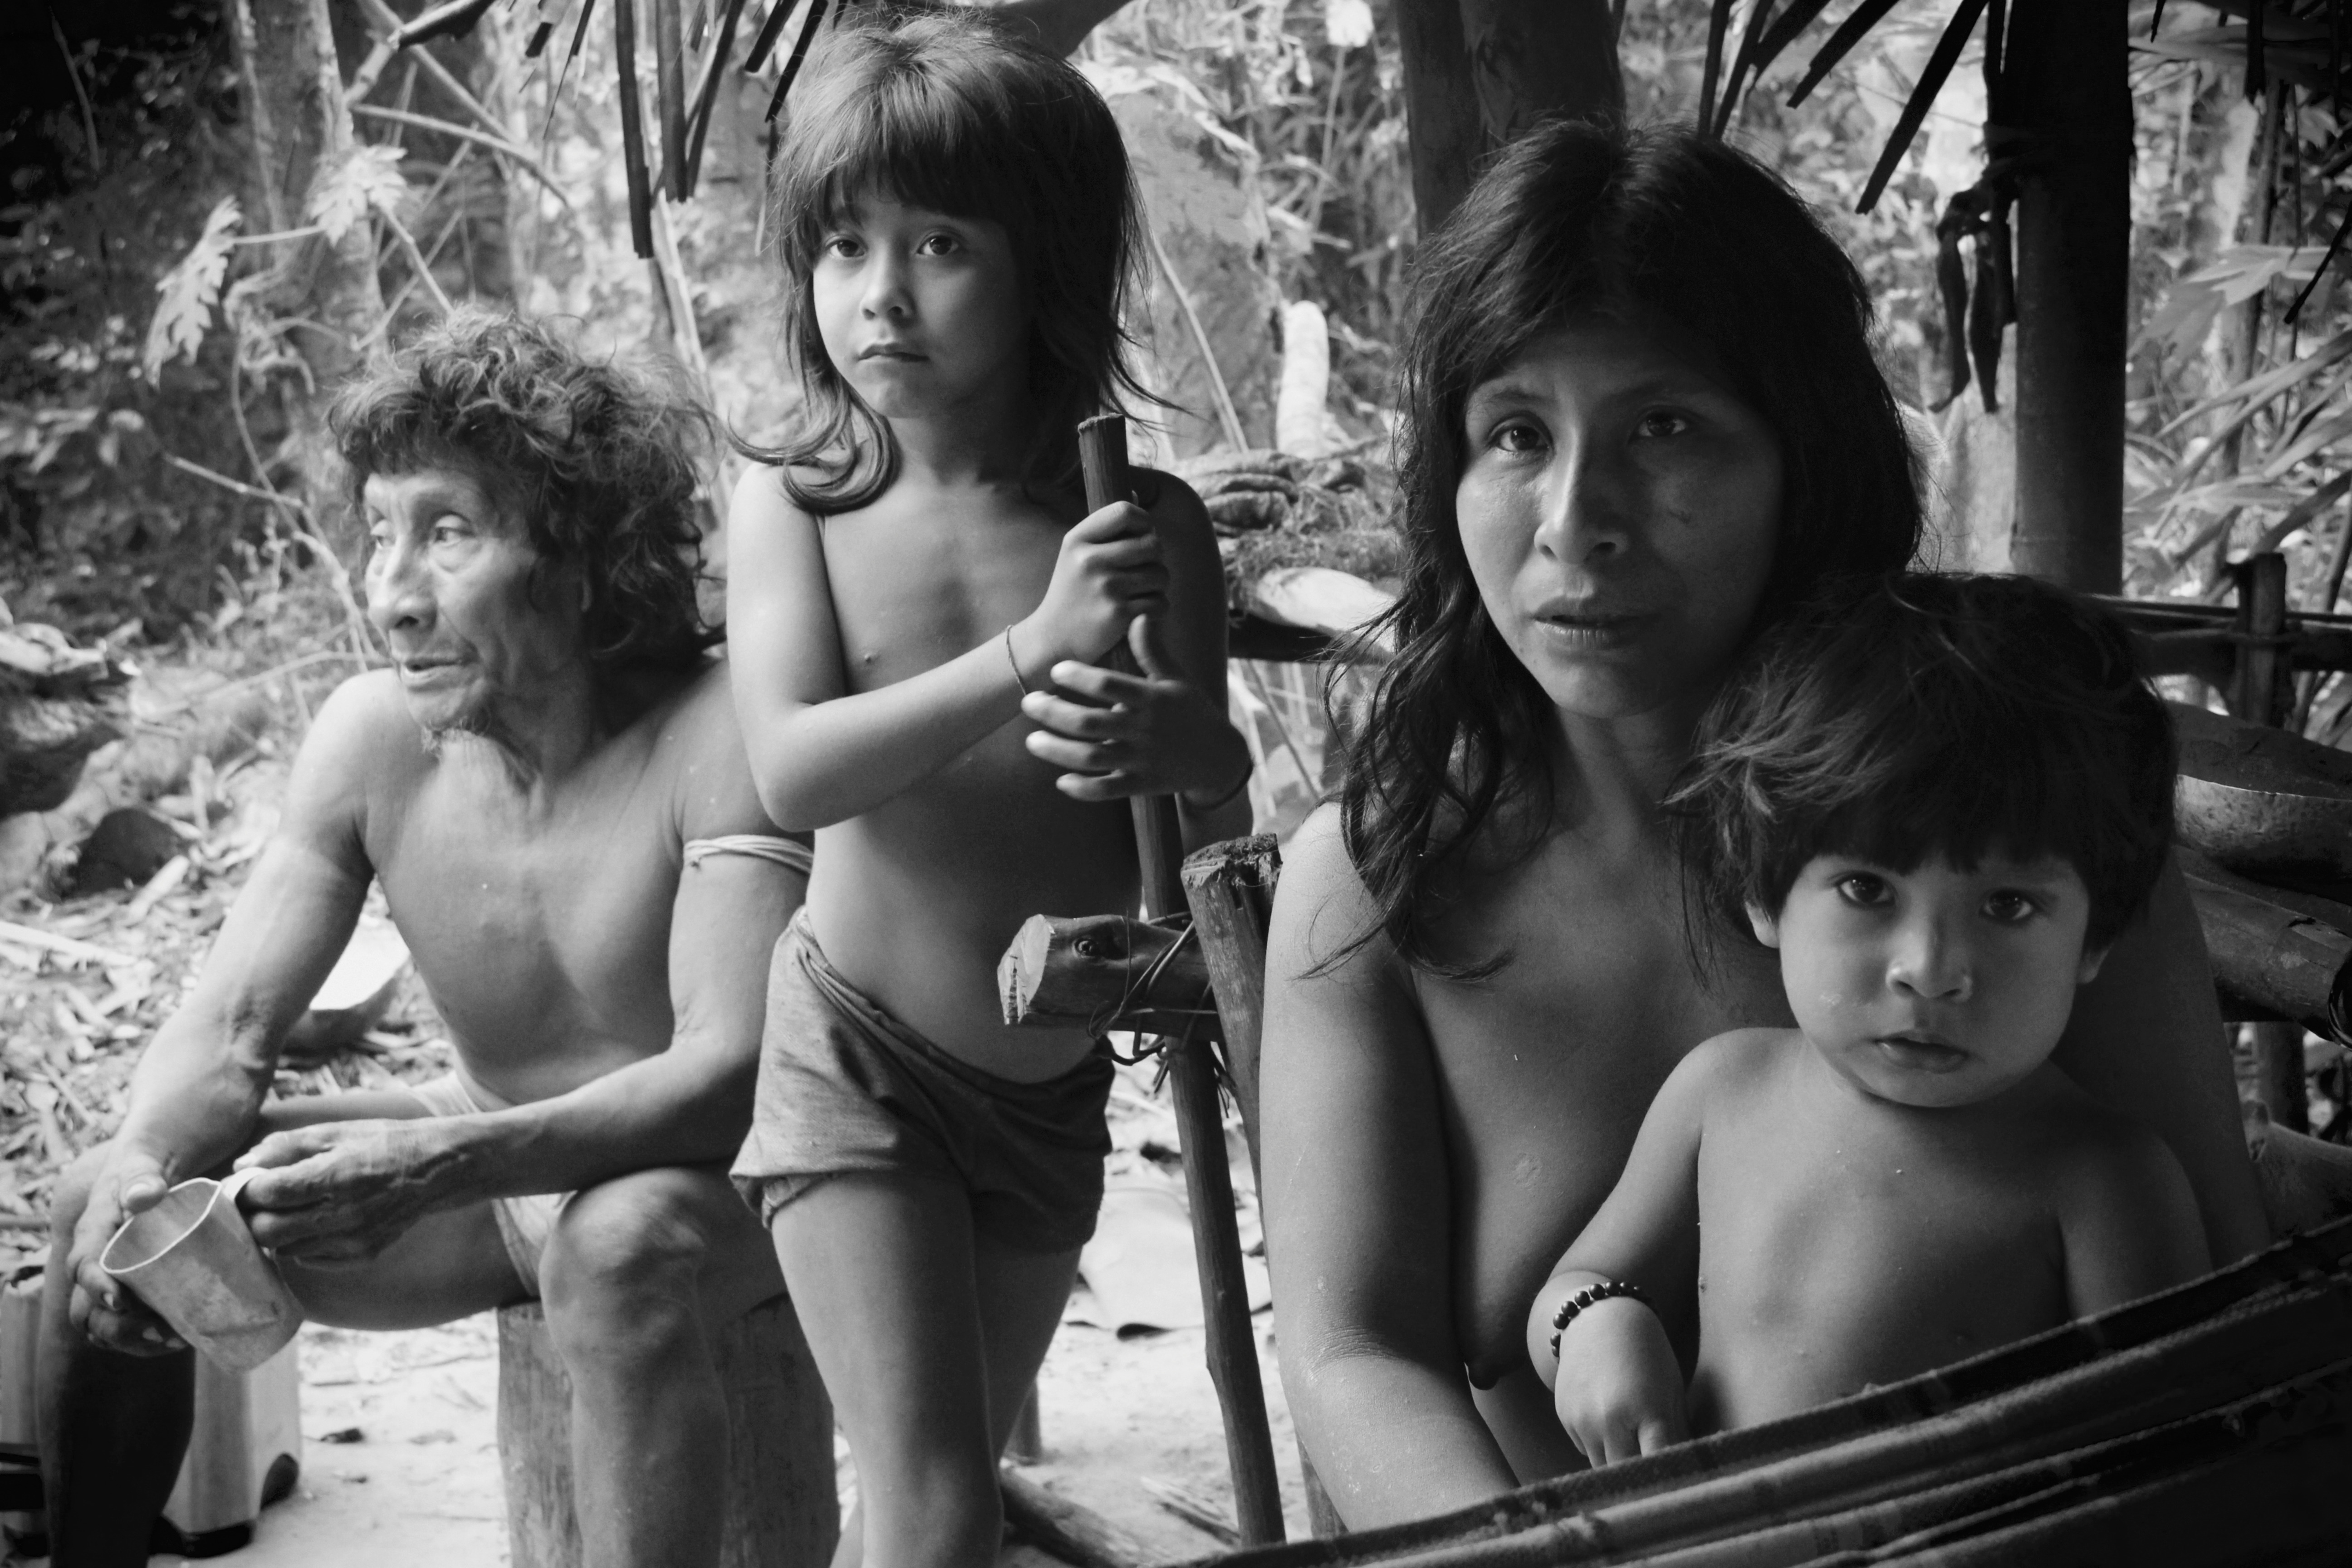
\includegraphics[width=\textwidth]{./imgs/IMG_4928}
%\caption{Pak'wa'ĩa com Manimya e Tokĩ, dois de seus filhos. Ao lado, seu sogro Pirama’a (aldeia Juriti, 2016).}
%\end{figure}

``Eu vou ficar com você!'', \textit{Ajku ta ni pyry}, ``Fique logo comigo!'', 
\textit{Ha ruku apaj}, foi o que disse a jovem Ipokaxi'ı͂a ao velho
Xiramua. Em 2013 ela estava com 12 anos e ``gostou'', \textit{maparỹ}, dele,
que já era um quinquagenário. A esposa anterior de Xiramua o havia
deixado, levando quatro dos seus cinco filhos; mudou-se para outra
aldeia para viver com um jovem de quem havia ``gostado'', ``se enamorado''.
Isto não é nenhuma raridade, e as mulheres guajá, que ainda se casam bem
novinhas --- \textit{awa xa'aruhua}, ``gente jovem'' ---, muitas vezes com homens
bem mais velhos, se cansam de tanta ``velharada'', \textit{wỹxa'atekera},
e deliberadamente trocam seus alquebrados esposos por homens jovens que,
assim relatam, serão melhores companheiros: jovens, bonitos, menos
rabugentos, mais produtivos na caça, dentre outros motivos que a
``mulherada'', \textit{awa wahykera}, defende. Desde a separação em 2012,
Xiramua andava cabisbaixo em sua aldeia. Havia conseguido se unir a uma
menina que rapidamente o abandonou, alegando ser ele ``velho demais'' para
se casar com ela --- \textit{ixa'akera}, ``muito crescido''. E voltou a ficar
sozinho. Até que a pequena Ipokaxi'ı͂a lhe fez a feliz proposta: ``Fica
logo comigo!'', \textit{ha ruku apaj}, em uma tradução literal, ``você pode
ficar logo comigo!''. Quando o pai da jovem relatou tais episódios,
disse-me: \textit{Xiramua mixa'a ta}, ``Xiramua vai criar (minha filha)''.
\textit{Mixa'a}, ``fazer crescer'', ``criar'', pensado para a relação
conjugal, é o mesmo verbo utilizado por pais que criam filhos e por
mulheres que criam filhotes de animais na aldeia.

A produção teórica sobre o ``parentesco no contexto amazônico'', entendido
de maneira ampla como ``uma abreviação cômoda para o que, na Amazônia,
seria mais bem chamado teoria da relacionalidade generalizada'' (Viveiros
de Castro, 2002c, p.\,422) --- a saber, as formas de aliança, produção de
pessoas e coisas, alternativas para um modelo genealogista-terminológico
---, concebe a afinidade como um símbolo que transcende o parentesco. Este
conceito, complementado pela sua contraparte, a consanguinidade, assume
formas variadas que ``não só determinariam outros referentes que os
nossos, como envolvem outros componentes'' (Viveiros de Castro,
2002c, p.\,407). O interesse atual demonstrado pela antropologia do
parentesco, cuja ``homonímia (com a noção euro-americana de parentesco)
visa ressaltar as diferenças, a despeito das semelhanças'' (Viveiros de
Castro, 2002c, p.\,407), tem produzido análises menos essencialistas com que
procura entender processos de vida, de pessoas que estão associadas
entre si, como parentes que ``participam intrinsecamente da existência
uma das outras'' (Sahlins, 2011, p.\,01). Embora tal ``relacionalismo'' não
esteja completamente ausente das análises clássicas, como lembra
Strathern (1995, p.\,12; 2006 {[}1988{]}, p.\,394), as relações de parentesco
foram redefinidas a partir de outros tópicos, tais como corpo, pessoa,
gênero e, no caso amazônico, da guerra, da predação, do comércio e do
xamanismo, em que desde o final da década de 1970 ``reconheceu-se a
necessidade de se forjar uma linguagem adequada à realidade etnográfica''
(Viveiros de Castro, 2002a, p.\,106).\footnote{Para uma importante discussão
  sobre o tema, ver Overing (1977).} Neste capítulo e no próximo,
examino as formas Guajá de conceber parentes e alianças apresentando uma
terminologia de relações sociais que envolve homens e mulheres, adultos
e crianças, e mesmo humanos e não humanos. Discuto aqui um sistema de
ação particular revelado pelo verbo \textit{riku} (ou \textit{ruku}, a
depender do falante), cujo principal efeito é a produção de relações
assimétricas de ``criação'' --- no sentido de ``cuidado'' e ``fazer crescer'' ---
não só entre pessoas em geral, \textit{awatea}, que atravessa diferentes
campos da experiência humana, mas também de animais e mesmo coisas.

Diante disto, podemos questionar: de que outras maneiras os antropólogos
conseguem discutir o parentesco em coletivos nos quais tal conceito,
assim como nós o concebemos, não está colocado? Como podemos pensar o
parentesco, mais especificamente o sistema de aliança em um grupo
ameríndio como os Guajá, quando boa parte do que formulam sobre isso se
encaminha a outras esferas que não a do parentesco? Por exemplo, para
definir uma relação conjugal, os Guajá mobilizam elementos diferentes
dos envolvidos em nosso próprio sistema e pensam o casamento com um
processo de ``criação''. Em termos mais diretos, a produção de cônjuges,
seja de homens ou mulheres, é coextensiva a outras relações que
usualmente escapariam ao campo do parentesco. Durante meus anos de
pesquisa, as pessoas constantemente definiam o fato de maridos e esposas
estarem ``juntos'', \textit{pyry}, morando na mesma casa e criando filhos,
com termos exatamente idênticos àqueles com que explicavam por que as
mulheres criam seus animais domésticos; ou por que cada qualidade de mel
está relacionada a seres ``donos do méis'' (como veremos aqui), ou mesmo
porque --- a partir de uma sensível percepção etológica --- diferentes
espécies de animais são muitas vezes encontradas juntas, ou ao menos
próximas umas das outras, como se determinado animal andasse junto de
outro. Quando o tema do parentesco surgia em minhas indagações, as
pessoas lançavam-no para fora do campo conceitual sobre o qual eu estava
confortavelmente instalado.

As ideias gravitavam em torno de ideias como \textit{mixa'a} --- ``criar para
filho'', ``criar para cônjuge'', ou ``fazer crescer'' ---, utilizadas
preferencialmente por mulheres. Formulada por elas, a frase era
\textit{jaha amixa'a ta hamenime}, que pode ser traduzida como ``eu vou
criá-lo para ser meu marido'', ou literalmente, ``Eu vou fazê-lo crescer
transformando-o em marido''. Da mesma maneira, um casamento que os pais
possam planejar para sua filha é referido pela frase \textit{mãj manã}, ou
seja, ``mandar, enviar para ele criar (a minha filha)''. E um homem à
procura de casamento costuma dizer a \textit{jaha amãj ta harimirikorime},
que pode ser traduzido simplesmente como ``Eu vou criá-la como esposa''. O
sufixo \textit{rime} (ou \textit{nime}, a depender da raiz à qual se anexa)
guarda uma função translativa que, como sugere a nomenclatura, indica
que o nome \textit{harimiriko}, ``minha esposa'', é o resultado de uma
transformação a partir da ação indicada pelo verbo, a qual que veremos
aqui. A tradução literal para esta frase seria, portanto, ``eu vou
criá-la transformando-a em minha esposa''.

Paralelamente a isso, os Guajá trazem um conceito de relação revelado
pelo verbo \textit{riku} (ou \textit{ruku}), central em sua socialidade, que
orienta a proximidade e a distância entre diferentes seres no mundo, no
sentido sociológico da afinidade potencial amazônica. Trata-se de um
processo contínuo de produção de novas relações entre pessoas (que
assinala a paternidade e a maternidade, por exemplo) e coisas (com a
posse de determinados objetos, por exemplo), encontrando-se ressonâncias
na conhecida ideia de ``familiarização'' da literatura da etnologia
sul-americana\footnote{Cf. Erikson, 1987, 2012; Fausto, 2001; Bonilla, 2005.} ou
``maestria'' (Costa, 2013; Fausto, 2008; Kohn, 2007), em que se envolvem
pessoas, plantas, animais, espíritos em relações que implicam ``donos'',
sendo muitos os exemplos em que isto ocorre.\footnote{Ver Bonilla, 2005;
Brightman, 2010; Cabral, 2012; Cesarino, 2010; Descola, 1986, 2006; Erikson,
1987; Fausto, 2008; Gallois, 1988; Hugh-Jones, 1996; Kohn, 2007; Lea, 2012;
Lima, 2005; Viveiros de Castro, 2002d, dentre outros.}

\begin{center}\adforn{68}\end{center}

Os dados da análise subsequente são, em sua maioria, extraídos de minha
experiência na aldeia do \textsc{pin} Juriti, constituída por uma população
pequena, sobrevivente de uma depopulação recente e, nos dias atuais, com
poucas mulheres ``casáveis'' disponíveis. As sequelas do processo de
contato, iniciado nos anos 1970 --- e até hoje inconcluso ---, estão muito
presentes na vida da aldeia do \textsc{pin} Juriti. Por isso, estudar relações de
parentesco em uma população tão reduzida significa testemunhar as
soluções (mais do que) criativas que as pessoas encontraram para manter
dignamente sua reprodução física e social. A aldeia Juriti foi
construída pela Funai, a partir do contato que, por sua vez, foi marcado
por uma grande perda da população adulta devido a gripe, malária e
tuberculose. Vários homens e mulheres, hoje em idade adulta, tornaram-se
órfãos, cerca de duas décadas atrás (a década de 1980 fora a mais
impactante para as vidas Guajá), quando foram contatados em 1989 e
incorporados a outras famílias. O modelo de grupos locais, que seguiam a
vida dispersos nos \textit{hakwaha}, se esfacelou, e o território agora é
definido pelo regime do Estado brasileiro. A população não indígena
avança (e continua) em direção às antigas áreas de caça. Grupos outrora
distintos e, até certo ponto, rivais foram obrigados a conviver em um
novo lugar, com pessoas, \textit{awa}, de cuja existência só sabiam por
ouvir falar, enquanto nem mesmo sabiam existir outros. As distâncias
ótimas entre grupos ``afins'', \textit{hapihianã}, cederam lugar à
hiperproximidade cognática, outrora experimentada apenas por
``consanguíneos'', \textit{hapihiara}, e que hoje se tornou regra dos novos
aglomerados populacionais. O clima fresco sentido na floresta cedeu
lugar à quentura da clareira. A imprevisibilidade das caçadas cotidianas
foi dividida com o extenuante e monótono \textit{trabalho} de sol a sol,
informado pela Funai. No lugar das casas construídas com folhas frescas
e que antes eram deixadas para trás, hoje encontramos moradias de
pau-a-pique, repletas de baratas e pó. Se a unidade da investigação do
etnógrafo é ``a vida social de alguma região do mundo durante um certo
período de tempo'', conforme definição de Radcliffe-Brown,\footnote{E aqui
  citado a partir de uma das três epígrafes de \textit{O Gênero da
  Dádiva}, de Marilyn Strathern (2006).} o caso em questão, o
parentesco guajá, é emblemático --- eu suponho --- por representar arranjos
temporários, por ser original --- e bastante original --- justamente por ser
temporário. Lembro também que o objetivo deste e do próximo capítulo não
é apresentar descritivamente as categorias, regras e práticas do sistema
de parentesco, mas produzir uma reflexão baseada nas formas Guajá de
relação e produção de parentes.

\section{simetrias e assimetrias}

Tal como esboçado no capítulo anterior, o universo dos parentes está
dividido entre os \textit{hapihiara}, ``cognatos'', e \textit{hapihianã}, ``não
cognatos'', ou ``aliados'', diferença baseada no gradiente de distância
(genealógica e socioespacial) entre ``parentes próximos'' (ou
verdadeiros) e ``parentes distantes'' (ou classificatórios), como já
discutido por outros autores.\footnote{Ver Viveiros de Castro, 2002a, p.\,121.}
Mesmo que as categorias \textit{hapihiara} e \textit{hapihianã} funcionem
distintamente, seu regime não está diretamente relacionado a uma
dicotomia automática refletida na oposição entre afins e consanguíneos. A
terminologia de relações Guajá (assim como outros casos amazônicos)
engloba (ou engole) as esferas do ``paralelo'' e ``cruzado'' (já criticadas
pela etnologia amazônica) e por vezes as embaralha. Estou longe de
sugerir que não haja diferenças entre membros ``casáveis'' e
``não casáveis''; ``parentes próximos'' e ``distantes''; contudo, aqui
também não é possível ``recortar de forma simples a terminologia em dois
domínios mutuamente exclusivos'' (Fausto, 1995, p.\,65).

No plano de uma alteridade global --- que prescreve relações do tipo
\textit{awa}, ``gente'', \textit{mihua}, ``selvagens'', \textit{awaetea}, ``gente de
verdade'', \textit{awa}, ``gente'', ou de uma diferenciação local,
intra-aldeã ---, a distinção sociológica entre cognatos e não cognatos ``de
natureza concêntrica e contínua'', que ``sobredetermina o cálculo de
classes da terminologia'' (Viveiros de Castro, 2002, p.\,123), se mostra
mais eficaz aos problemas aqui observados do que consanguíneos/\,paralelos
e afins/\,cruzados. \textit{Hapihianã} se refere aos afins atuais com quem
se ``trocam cônjuges'' --- terceiros incluídos que modulam as posições de
consanguíneos e afins (Viveiros de Castro, \textit{op.\,cit.}, p.\,157).

\section{terminologias}

Tal como ocorre com outros povos nas terras baixas da América do Sul
(como os Parakanã, Trio, Cinta Larga, Panaré), os Guajá apresentam uma
terminologia de parentesco de variante dravidiana (ou de cruzamento tipo
``\textsc{a}'', de acordo com Trautmann-Barnes, 1998), marcada por equações
transgeracionais e preferência avuncular na regra de casamento.\footnote{Também
  conhecidos como de ``duas seções'' ou ``duas linhas'', o sistema de
  parentesco dravidiano foi originalmente descrito por Louis Dumont, em
  1953, e referido aos povos da Índia do Sul. Devido a inúmeras
  semelhanças, algumas ideias referentes a esses povos foram estendidas
  à paisagem amazônica (ver Viveiros de Castro, 2002a: 89--93). A
  ``questão dravidiana'', ou o ``dravidianato'', na Amazônia --- seu
  aparecimento na bibliografia especializada, desenvolvimento, e
  rendimento --- consta em importantes análises teóricas e etnográficas e
  dispensa maiores comentários neste livro (para um estudo de caso, ver
  Silva, 1995 e Taylor, 1998; para um balanço teórico, ver Viveiros de
  Castro, 2002; Trautmann \& Barnes, 1998). Grosso modo, o dravidianato
  é um regime de aliança que prescreve a fusão bifurcada (\textsc{f} = \textsc{fb} ≠ \textsc{mb})
  com a divisão diametral dos parentes em duas classes opostas: os afins
  e os consanguíneos.} O sistema de parentesco Guajá foi bem descrito
por Cormier, cuja análise comprova a ênfase oblíqua nas preferências
matrimoniais (2003, pp.\,57--84). A autora propõe uma terminologia do tipo
dravidiana-avuncular, cuja preferência no casamento com \textsc{zd}\footnote{Seguindo
  outros autores, utilizo as abreviações da notação inglesa para as
  posições genealógicas: \textsc{f}, pai; \textsc{m}, mãe; \textsc{s}, filho; \textsc{d}, filha; \textsc{b}, irmão; \textsc{z}, irmã; \textsc{h}, marido; \textsc{w}, esposa. E para termos compostos,
  leia-se de trás para frente: \textsc{mb}, irmão da mãe; \textsc{fm}, mãe do pai; \textsc{fzd}, filha da irmã do pai.} é complementada por outras alianças também oblíquas.

Cormier observa que o casamento preferencial é o de um homem com a filha
de sua irmã (\textsc{zd}), porém, a esposa também pode ser \textsc{zdd} e \textsc{zddd}, se essas
não forem filhas de ego {[}masculino{]} certamente. E do ponto de vista feminino,
isso implica o casamento com \textsc{mb}, \textsc{mbs}, se não for filho de ego {[}feminino{]} e
\textsc{mbss}. A autora apresenta então as principais características do sistema:

\begin{enumerate}

\item Preferência avuncular 
\item Poliginia (eu acrescentaria, com ênfase sororal) e poliandria 
\item Múltipla paternidade como (in)definidor da descendência  
\item Amnésia genealógica no registro da ascendência, em alguns casos, a partir da geração \textsc{g}+1 
\item Múltiplos padrões de residência (a variar pelos arranjos, idades dos cônjuges e outros fatores), porém com contornos neolocais 
\end{enumerate}

Além dos tópicos acima, acrescento à lista: 

\begin{enumerate}
\item Um importante operador de distância (\textit{kin distance}) que informa as posições \textit{hapihiara} e \textit{hapihianã}
\item Tendência levirática (o casamento com ``viúva'' de um irmão morto, para ego masculino) 
\item Ausência de qualquer parâmetro de idade relativa que informe o casamento com \textsc{zd}, diferentemente de outros casos Tupi-Guarani (como os Parakanã), em que prevalece a aliança avuncular (oblíqua) sobre a caixa dravidiana (horizontal) 
\item A inexistência de termos para primos cruzados,\footnote{Ver Fausto, 1995, p.\,68.} que no caso Guajá é preenchida por diferentes equações que obedecem a parâmetros associados à distância genealógico-espacial 
\item E, finalmente, a conversão terminológica da sogra (\textsc{wm}) em irmã (\textsc{z}), independentemente da relação pré-existente entre ego e sua sogra. Em suma, o sistema Guajá é delineado pela endogamia dos grupos locais com \textit{alianças curtas avunculares e patrilaterais}\footnote{Viveiros de Castro, \textit{op.\,cit.}, p.\,157.} 
\end{enumerate}

O embaralhamento genealógico, típico dos sistemas avunculares, ocorre na
relação entre os primos cruzados, oblíqua por excelência. Ego feminino refere-se a \textsc{zd}, \textsc{fzd} e \textsc{mbd} por \textit{imirikoa}, o termo para esposa,
enquanto ego masculino refere-se a \textsc{mb}, \textsc{fzs} e \textsc{mbs} pelo termo \textit{imena},
``marido''. Tais posições podem oscilar, a depender da sorte de arranjos
realizados. Isso faz com que os primos cruzados permaneçam em um campo
de alguma incerteza. No caso de ego masculino, as esposas em potencial são:
\textsc{zd}, \textsc{fzd} e \textsc{mbd}; e no caso de ego feminino, os maridos em potencial são: \textsc{mb},
\textsc{mbs} e \textsc{fzs}. Assim, para a mulher, ainda que potencialmente, a obliquidade
se dá no casamento com um homem de G\textsubscript{+1} (com \textsc{mb}), ao
passo que no caso do homem, em G\textsubscript{-1} (com \textsc{zd}). No sistema
de aliança guajá e nos avunculares em geral, os cônjuges podem aparecer
em G\textsubscript{+1}, G\textsubscript{0} e G\textsubscript{-1}; e,
assim como outras terminologias do continente, a terminologia guajá
também está baseada em ``equações transgeracionais que afetam as
posições cruzadas de G\textsubscript{0}'' (Fausto, 1995, p.\,68). Os
\textit{Tupi} Guajá, portanto, se encaixam em um pequeno grupo de povos
que oferecem a ``ilustração mais clara da variante patriavuncular de
troca simétrica. Se em muitos grupos da família tupi-guarani o casamento
entre tio materno e sobrinha é uma união secundária (em geral associada
à poliginia de homens importantes) ou uma `infração preferencial' a uma
norma bilateral'', em grupos como os Guajá o ``casamento com a filha de \textsc{zd}
é não só preferencial como muito comum, produzindo-se quase que somente
inflexões oblíquas na terminologia'' (Viveiros de Castro e Fausto, 1993,
p.\,157).

Retomando o episódio com que iniciei esse capítulo, Xiramua, na época
com 52 anos, estava em vias de se casar com Ipokaxi'ı͂a, de 12 anos,
porque sua esposa anterior, Jauxika --- 28 anos na época, e mãe de seus
cinco filhos ---, o largara por um rapaz de 14 anos. Durante um período
fora de casa, Jauxika argumentou querer viver com o jovem Takwari na
aldeia Juriti, sugerindo que Xiramua voltasse a viver em sua aldeia de
origem, sem ela nem os filhos. Foi esta separação que fez com que
Xiramua sofresse de tristeza, \textit{kije}, e procurasse por outra
esposa. O casamento de Xiramua com sua ex-mulher foi desfeito para ambos
recomeçarem uniões com cônjuges de gerações descendentes. Em uma imagem
um tanto forçada, é como se os Guajá não concordassem com dois jovens se
casarem diretamente (muito embora o façam com mais frequência nos dias
atuais), mas tivessem que o fazer com pessoas de gerações diferentes;
ou, é como se a diferença etária fosse a principal forma de mediação de
uma troca matrimonial. Observo não apenas aquilo que Lévi-Strauss (1982
{[}1967{]}, p.\,404) afirmou ser um ``desprezo pela noção de geração'', ao
comentar um antigo trabalho sobre os Miwok, mas uma preferência radical
pelo casamento oblíquo, que nem sempre ocorrerá com a filha da irmã
(\textsc{zd}), como sabemos dos sistemas oblíquo-avunculares (como um paralelo
Jê, ver Schroeder, 2006, pp.\,157--160). Os Guajá fariam parte daquilo que
Viveiros de Castro (2002a, p.\,113, nota 8) mencionou como ``avunculares sem
complexo'', ao lado dos Tupinambá, Parakanã e Mondé, em oposição àqueles
povos nos quais o casamento avuncular --- embora uma possibilidade real ---
aparece, segundo os etnógrafos, como um desvio das normas, ``uma união
semilícita, semi-incestuosa'', parte incestuosa, porém ``apetitosa'', diria
Rivière (1969, pp.\,190--191).

Quanto à terminologia, sigo aqui as sugestões de Cormier (2003). Em
linhas gerais, a autora encontrou quatro tipos de casamento: 

\begin{enumerate} 
\item O de ego masculino com a filha da irmã mais velha \textsc{zd}: este detém a primazia
\item O casamento com \textsc{zdd} (= \textsc{wd}, se não for a filha de ego)
\item Casamento com \textsc{zddd} (= \textsc{wbd}), com a ``neta'' da esposa: neste caso, ego masculino
casa-se com a filha do seu cunhado (que, por ser ``cunhado'' (\textsc{wb}) de
ego, casou-se com a filha deste), e também ``neta'' de sua esposa
\item O casamento com prima cruzada patrilateral (= \textsc{fzd} a mesma posição de ``\textsc{m}''){Cormier, 2003, p.\,60.}
\end{enumerate}

% Verificar tabela
% \begin{table}[H]
% \centering

% \label{my-label}
% \begin{tabular}{|l|l|}
% \hline
% \textbf{Ego Masculino} & \textbf{Ego Feminino} \\ [0.5ex] 
% \hline\hline
% \textsc{m = fzd}                & \textsc{m = fzd}               \\ \hline
% \textsc{mb = fzs}               & \textsc{mb = fzs = marido}     \\ \hline
% \textsc{zd = mbd = esposa}      & \textsc{s = mbs}; \textsc{d = mbd}\footnotemark      \\ \hline
% \end{tabular}
% \end{table}
% \footnotetext{Fonte: Cormier 2003.}

% Verificar tabela (vai até Referência dos indivíduos do diagrama)
% Na aldeia Juriti, especificamente, entre 16 casamentos no ano de
% 2008\footnote{Refiro-me aos casamentos entre os indivíduos (17--16;
%   22--16; 11--30; 27--8; 6--8; 12--2; 22--20; 20--28; 2--31; 21--26; 7--23; 1--32;
%   19--32; 4--40; 3--33; 5--25)} encontramos cinco que compreendem a união de
% um homem com a filha de sua irmã (\textsc{zd}), como vemos abaixo.

% %\includegraphics[width=7.41667in,height=5.25in]{media/image1.wmf}%

% %Figura6%

% \begin{figure}[t] %sidewaysfigure
% %\thisfloatpagestyle{empty}
% \centering
%   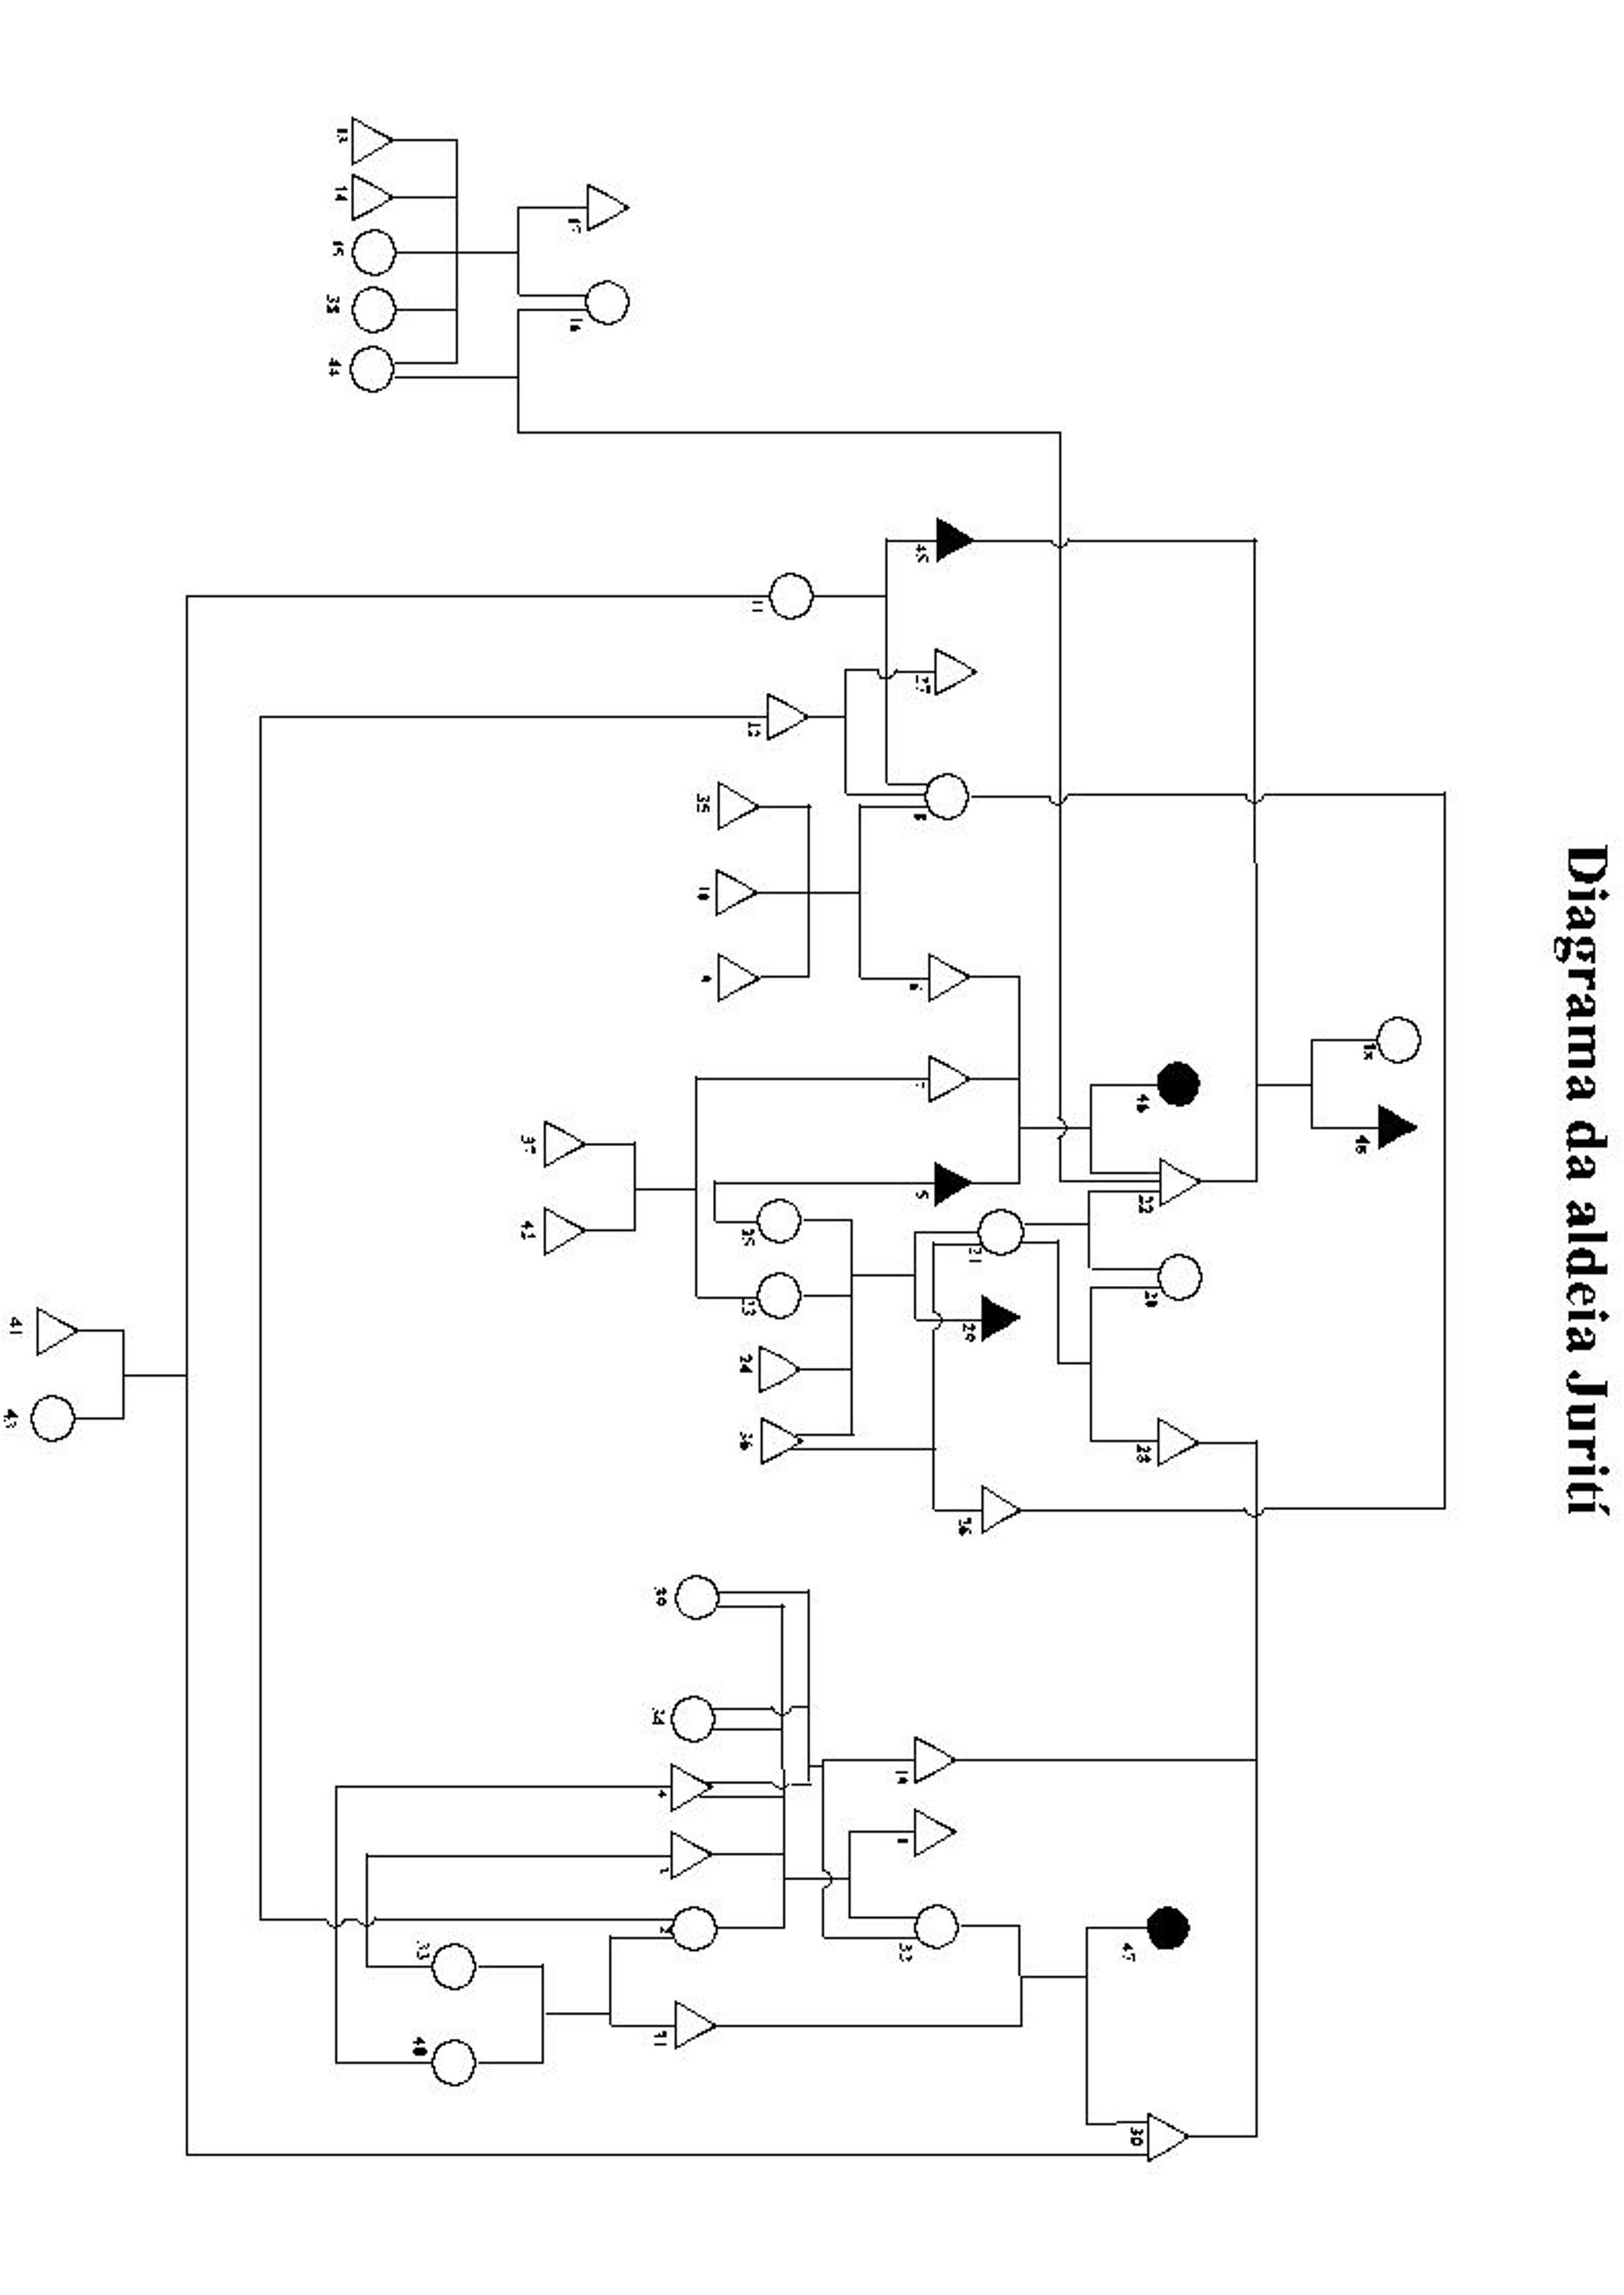
\includegraphics[width=\textwidth]{./imgs/Figura_6b}
%   %\hfill
% \end{figure}

% \pagebreak
% \noindent\textbf{Referência dos indivíduos do diagrama}

% \begin{multicols}{3}
% \begin{enumerate}
% \setlength\itemsep{0em}
% \item Kamara
% \item Pakwa
% \item Juma
% \item Kiripitỹa
% \item Pinawãxa
% \item Wirahoa
% \item Hajmakoma
% \item Ajruhua
% \item Juwi
% \item Takwaria
% \item Panapinuhũa
% \item Juxa
% \item Kiipia
% \item Arawatỹa
% \item Takwariropitỹa
% \item Hakoĩa
% \item Takwarẽxa’a
% \item Amerixa’a
% \item Xiparamỹxa’a
% \item Amỹ
% \item Amỹ
% \item Muturuhũa
% \item Panyxĩa
% \item Kaawi
% \item Aparana
% \item Juriximatỹa
% \item Kamaraxa’a
% \item Takya
% \item To
% \item Pira’ima
% \item Pirama
% \item Panyxĩa
% \item Aparanỹa
% \item Mimijawa
% \item Jahara
% \item Makoraia
% \item Manaixa
% \item Tymiri
% \item Aparikya
% \item Para
% \item Majakatỹa
% \item recém
% \item ``-''
% \item ``-''
% \item Iharoa
% \item ?
% \item Panyxĩa
% \item ?
% \end{enumerate}
% \end{multicols}


\begin{comment}
\begin{table}[H]
\centering
\caption{Referência dos indivíduos do diagrama}
\label{my-label}
\begin{tabular}{|l|l|l|l|}
\hline
\textbf{Nº} & \textbf{Indivíduo} & \textbf{Nº} & \textbf{Indivíduo} \\ \hline
\textbf{1}  & Kamara             & \textbf{25} & Aparana'ia         \\ \hline
\textbf{2}  & Pakwa'ĩa           & \textbf{26} & Juriximatỹa       \\ \hline
\textbf{3}  & Juma'ã             & \textbf{27} & Kamaraxa’a         \\ \hline
\textbf{4}  & Kiripitỹa         & \textbf{28} & Takya              \\ \hline
\textbf{5}  & Pinawãxa'a         & \textbf{29} & To'oa              \\ \hline
\textbf{6}  & Wirahoa            & \textbf{30} & Pira’ima'ã         \\ \hline
\textbf{7}  & Hajmakoma'ã        & \textbf{31} & Pirama'ã           \\ \hline
\textbf{8}  & Ajruhua            & \textbf{32} & Panyxĩa           \\ \hline
\textbf{9}  & Juwi'ia            & \textbf{33} & Aparanỹa          \\ \hline
\textbf{10} & Takwaria           & \textbf{34} & Mimijawa           \\ \hline
\textbf{11} & Panapinuhũa       & \textbf{35} & Jahara             \\ \hline
\textbf{12} & Juxa'a             & \textbf{36} & Makoraia           \\ \hline
\textbf{13} & Kiipia             & \textbf{37} & Manaixa'a          \\ \hline
\textbf{14} & Arawatỹa          & \textbf{38} & Tymiri'ixa'a       \\ \hline
\textbf{15} & Takwariropitỹa    & \textbf{39} & Aparikya           \\ \hline
\textbf{16} & Hakoĩa            & \textbf{40} & Para'ia            \\ \hline
\textbf{17} & Takwarẽxa’a       & \textbf{41} & Majakatỹa         \\ \hline
\textbf{18} & Amerixa’a          & \textbf{42} & recém-nascido      \\ \hline
\textbf{19} & Xiparamỹxa’a      & \textbf{43} & ``-''                \\ \hline
\textbf{20} & Amỹ Pirawia       & \textbf{44} & ``-''                \\ \hline
\textbf{21} & Amỹ Pirahỹ       & \textbf{45} & Iharoa             \\ \hline
\textbf{22} & Muturuhũa         & \textbf{46} & ?                  \\ \hline
\textbf{23} & Panyxĩa           & \textbf{47} & Panyxĩa           \\ \hline
\textbf{24} & Kaawi'ia           & \textbf{48} & ?                  \\ \hline
\end{tabular}
\end{table}
\end{comment}

Pelo cálculo avuncular Guajá, \textsc{zs} é um ``cunhado'', ao passo que \textsc{mb} é
"sogro", ambos sendo referidos pelo mesmo termo, \textit{hawaja} (ou
\textit{harawaja,} na primeira pessoa); ambos são afins em uma posição
intermediada pela esposa de ego. Além disso, a distinção entre sogro e
cunhado parece não ser produtiva aqui, uma vez que um homem
frequentemente se casa com uma mulher e cede sua filha para o irmão
dessa mesma mulher, fazendo com que ``sogro'' e ``cunhado'', muitas vezes,
ocupem literalmente a mesma posição.

Embora encontremos com os Guajá muita camaradagem entre um homem e seu
sogro, é na relação com a sogra-irmã que um homem investe seu trabalho,
uma vez que alimentar uma jovem esposa (que ainda pode estar morando na
casa de sua mãe) é alimentar também a mãe dela e seus irmãos menores.
Depois que a jovem passa a viver com o marido, esse fornecimento de
comida tende a diminuir drasticamente, mas não é raro os homens,
atendendo a pedidos, continuarem caçando esporadicamente para seus
sogros, e hoje em dia, participarem diretamente das atividades de roça
de seus sogros. Isso pode ser entendido como um \textit{serviço da noiva},
embora também encontremos entre os Guajá um \textit{preço da noiva} (uma
vez que serviços como roça, trabalhos de montagem de casas e outros não
eram feitos pelos Guajá até o contato), que deve ser pago com comida
(peixes, carnes, frutos e, atualmente, farinha) e outras cortesias (como
os bens manufaturados que venham a conseguir), como já demonstrado por
Cormier (2003, p.\,49). A duração dessas obrigações é difícil de precisar.
Um genro, mesmo após ter se casado e tido filhos, pode --- ou não ---
continuar levando caça para o pai e mãe da mulher durante muitos anos
ainda, porém com menos intensidade do que à época em que ela vivia na
casa de seus pais.

Como sabemos sobre a terminologia avuncular, os sobrinhos, irmãos da
esposa são cunhados que serão convertidos em genros, bem como o tio
materno é uma espécie de cunhado que se transformará em sogro (Dal Poz,
\textit{op.\,cit.}, p.\,54). Ou se preferimos, como defende Fausto, ``as irmãs são
não afins \textit{sui generis}, pois seu destino é serem sogras {[}\ldots{}{]}: do
ponto de vista feminino, o genro é um irmão; do ponto de vista
masculino, a irmã é uma sogra'' (Fausto, 1995, p.\,80). E, ``ao nível da
representação, a consanguinidade da irmã engloba a afinidade da sogra'',
porém, ``ao nível do funcionamento do sistema, importa que a irmã se
realize enquanto sogra''.\footnote{\textit{Idem}.} Entre os Guajá, por sua vez, o que se
mantém é o laço entre cunhados (ego e \textsc{wb}), representado pelo termo
recíproco \textit{hawaja}, cuja expressão vocativa é \textit{haxa'ỹ}. Um
homem adulto cujo cunhado é um rapaz jovem pode fazer as vezes de
instrutor de caça e, tal como um \textit{pai}, manter o jovem sob sua
guarda a fim de o formar nas atividades masculinas (caça, canto,
construção de casas, dentre outras). Caso cunhados adultos sejam da
mesma faixa etária, costuma haver uma grande camaradagem entre eles que,
juntos, realizam essas atividades. Tal relação se prolonga, uma vez que
o irmão da esposa sempre terá interesse nas filhas, pensadas como
esposas (\textsc{zd}), que sua irmã poderá produzir. É comum um homem dizer ao
cunhado (\textsc{wb}) ``vou fazer uma esposa para você'', referindo-se à própria
filha. Portanto, \textit{hawaja} é muito mais alguém ligado à irmã-sogra
(como o filho dela \textsc{zs} ou marido \textsc{zh}) do que uma categoria genérica de
afinidade simétrica. Se \textit{hawaja} qualifica a relação entre um homem
e seus afins próximos se aplicando a diversas posições (\textsc{wf}; \textsc{wb}; \textsc{mb}; \textsc{zs}),
sugere que, entre os Guajá, a afinidade e as prestações de casamento
passam fundamentalmente pela sogra-irmã.

Em anexo, apresento um diagrama do casamento avuncular em que evidencio
os termos vocativos e referentes em cada um deles.

\section{\textit{hawirokaha kĩa}}

Os termos vocativos do parentesco também são pensados como
\textit{hawirokaha kĩa}: aqueles pelos quais todos são chamados e que,
quase sempre, fazem as vezes do nome. Como já observei, o termo
\textit{hapihiara} é utilizado tanto para homens quanto para mulheres que
tenham laços de parentesco estreitos, sejam germanos de ambos os sexos,
pais e filhos, ou demais indivíduos impedidos de se casarem entre si; ao
mesmo tempo que \textit{hapihianã} são todos os outros de uma aldeia. Na
forma vocativa, a distinção é expressa pelos termos \textit{xa'a}, ``cognatos'', 
e \textit{xia}, ``não cognatos''. Os Guajá não reservam um termo
vocativo específico para esposa (\textsc{w}) e marido (\textsc{h}), mas sim um conjunto
deles. Para uma mulher, seu marido é usualmente chamado de \textit{xipa}
(o mesmo que para ``pai''), ou \textit{xipa'i}, ``papaizinho''; mas pode
ser chamado por \textit{haxa'a}, ``meu parente próximo'', ou pelo nome
próprio. Um homem pode chamar sua esposa por \textit{xa'ỹ} ou
\textit{xa'hũ}, em ambos os casos são termos muito carinhosos para esposa,
que também poderá ser chamada de \textit{amỹ} (o mesmo que para ``mãe'') e,
dependendo do caso, de maneira muito despretensiosa, até mesmo
\textit{xikari} (o termo reservado a cognatos de sexo oposto como
``irmãs''). Os vocativos \textit{haxa'a} (meus filhos); ou \textit{xipa}, ``pai''; 
\textit{xipa'i}, ``meu marido'', ou ``papaizinho''; \textit{xa'ỹ} ou
\textit{xa'hũ}, ``esposa''; e \textit{amỹ}, ``mãe'', são fundamentais para o
entendimento da vida.

\textit{Haxa'a} --- O pronome clítico de primeira pessoa \textit{ha}, 
``meu'', associado ao vocativo de cognação \textit{xa'a}, portanto
\textit{haxa'a}, ``meu \textit{xa'a}'', é a forma apropriada pela qual pais e
mães se dirigem aos filhos, independentemente do sexo de cada um.
Tratam-se por \textit{haxa'a} pais (\textsc{f}, \textsc{m}) e filhos (\textsc{c}h); avôs e netos; e
germanos do mesmo sexo. Muito utilizado no trato diário, \textit{haxa'a},
pode ser definido como o termo vocativo que exprime mesmas lateralidade
e substancialidade. Porém, é como termo de cognação (e não
consanguinidade) que é melhor apreendido. Por exemplo, o tratamento mais
comum entre um casal com filhos é pelos termos \textit{xipa} (\textsc{f}) e
\textit{amỹ} (\textsc{m}), respectivamente, porém, na intimidade de uma casa, homem
(\textsc{h}) e mulher (\textsc{w}) podem se tratar pelo recíproco \textit{haxa'a}. Da mesma
forma, em um casamento recém-arranjado de um homem adulto com uma menina
de pouca idade (com sete anos, por exemplo), o marido pode tratá-la por
\textit{haxa'a}, enquanto a menina o evoca por \textit{xipa} (\textsc{f}).\footnote{Tal
  tratamento tende a sofrer modificações após o crescimento da esposa,
  que passa a ser chamada por \textit{amỹ} ou mesmo por seu nome próprio,
  embora possam continuar utilizando o \textit{haxa'a}, porém com menos
  frequência.} Afins próximos também podem se tratar por \textit{haxa'a}
a depender das combinações matrimoniais e diferenças de idade
envolvidas. Por ser de uso cotidiano, é comum utilizarem a forma
\textit{haxa'a} acompanhada do nome próprio, como: \textit{haxa'a} Takwari,
\textit{aju} ``meu filho Takwari, venha cá''. Um pai (\textsc{f}) pode ser chamado de
\textit{ixa'akera}, um termo de difícil tradução, algo próximo a ``(já)
tornado um parente próximo (de alguém)''; ou ``alguém que se tornou pai'',
ou mesmo, ``crescido'', literalmente: \textit{i} mais \textit{xa'a} mais \textit{kera} é igual 1.
%\noindent prefixo de terceira pessoa (``dele'') + cognato + sufixo de atualização nominal retrospectiva.

Além desses usos, a ideia de cognação manifestada pelo termo \textit{xa'a}
--- que embaralha na mesma categoria relações próximas, sejam elas de
afinidade ou consanguinidade --- afeta a composição dos nomes próprios,
\textit{hawirokaha} ou ``nome dele(a)'', que no contexto Guajá tem como
principal função relacionar os humanos (nominados) a diferentes seres,
como veremos mais abaixo. Portanto, um indivíduo chamado Juxa'a é dito
ser parente da palmeira \textit{ju}, ``parente da palmeira marajá'' --- \textit{ju} mais 
\textit{xa'a} ---; e o nome Majhuxa'a é traduzível por parente da \textit{majhu} ou ``parente da jiboia'' ---- \textit{majhu} mais \textit{xa'a}.

Além disso, dois germanos de mesmo sexo, \textit{xa'a}, podem ser
considerados \textit{ikaena} \textit{xa'a},\footnote{\textit{Osso} mais \textit{xa'a}.} outra
forma de se referirem à germanidade, cuja tradução pode ser ``irmãos de
osso'', devido à hiperproximidade \textit{cognática} dos indivíduos, algo
próximo ao que na tradição ocidental se denominaria \textit{irmãos de sangue}.

Nessa hiperproximidade, o vocativo de extremo carinho de uma mãe para
seus filhos, meninos e meninas, é \textit{Sukúa}, cuja tradução mais
simples é ``meu filinho'' ou ``minha filinha'', usado para crianças pequenas.
Uma vez os filhos crescidos suas mães chamam os rapazes de \textit{Taxí}, ``filho crescido, grande'' e as moças de \textit{Xa'ahũ}, ``filha crescida, grande''.

\textit{Xipa} e \textit{amỹ} --- Embora o termo referente a marido
seja \textit{imena}, a mulher frequentemente chama o seu \textit{imena} pelo
termo \textit{xipa} (a pronúncia é ``\textit{txipá''}), o mesmo usado para
``pai'' (\textsc{f}/\,\textsc{fb}), ao passo que um homem, não menos frequentemente, chama
sua esposa por \textit{amỹ}, o termo para ``mãe'' (\textsc{m}).

É muito comum uma esposa se referir ao marido por \textit{xipa}. Além
desse, pai e homens mais velhos, em diversas situações, são tratados
pelo termo. Uma tradução correta para \textit{xipa} pode ser ``homem
adulto'', seja ele velho ou não. Além de esposos, são \textit{xipa}: 

\begin{enumerate}
\item Um pai em relação a um filho ou filha 
\item Avôs em relação aos netos, que
também podem ser chamados de \textit{xipa}\textit{tamỹ}, ``pai velho'' ou
``chefe'' 
\item Um homem para a esposa 
\item Todos os homens mais velhos,
independentemente do grau de parentesco com a pessoa que o denomina
\end{enumerate}

Além desses, os Guajá se referem aos \textit{karaia} mais próximos --- como
os funcionários da Funai --- por \textit{xipa}, além de a mim mesmo que,
desde muito cedo em campo, passei a ser chamado por esse termo seguido
pelo meu nome: ``\textit{xipa} Uirá''. Esta minha designação começou pelas
crianças, passou pelos jovens, e hoje todos me chamam dessa forma. Pode
inclusive, como neste caso, acontecer de homens mais velhos chamarem
alguns mais jovens por \textit{xipa}. Por exemplo, Muturuhũa é pai de
Hajmakoma'ã e, algumas vezes, principalmente na floresta durante as
caçadas, Muturuhũa chama o filho por esse termo, o que não quer dizer
que ele estivesse chamando seu filho de ``pai''. Neste caso é um
tratamento dado a homens já adultos, também utilizado para se referir ao
pai (\textsc{f}). O termo para homens muito mais velhos, os avós, por exemplo, é
\textit{xipa tamỹ}, e este último termo é o mesmo que exprime a ideia de
``chefe'' para os \textit{awatea}. O nome de parentesco utilizado para
``pai'' é \textit{tu} (ou \textit{tua}). Tanto \textsc{f} quanto \textsc{fb} são chamados por
\textit{xipa}, porém no que tange ao referente \textsc{f} é \textit{tu} e \textsc{fb}
\textit{tunã}, o que também é traduzido algo como ``pai com menos
intensidade''.

O termo \textit{amỹ} é utilizado por homens e mulheres para se referir a
mulheres a partir de \textsc{g}+1, sejam mães (reais ou classificatórias) ou
outras mulheres que ocupem essa posição. Tal como \textit{xipa}, é um
termo de grande amplitude: 

\begin{enumerate}
\item Uma mulher ou homem se refere a sua mãe
(\textsc{m}), tias (\textsc{mz}) e avós (\textsc{mm}, \textsc{fm}) por \textit{amỹ} 
\item Pode ser utilizado
por um homem na intimidade para se referir à esposa; 
\item No trato
diário, um homem também pode utilizar esse termo para se referir a
mulheres que ele não considera \textit{xikari} (\textsc{z}), sejam afins ou
consanguíneas
\item Mulheres que venham a conviver entre os Guajá, como
as auxiliares de enfermagem da Funasa, também são chamadas \textit{amỹ}.
Trata-se de um termo de grande amplitude que, tal como \textit{xipa}, pode
denotar uma relação de afinidade (próxima, como esposa), de
consanguinidade (como mães), ou ser utilizado em diferentes situações
\end{enumerate}

\section{casamentos}

Se observarmos a terminologia Guajá, comparando-a com a dos Parakanã,
não encontraremos entre os primeiros qualquer termo que sirva de
parâmetro para a idade relativa determinante nas escolhas matrimoniais.
Cormier defende que, à diferença dos casos Parakanã e Tirió, o
avunculato guajá parece não adotar regras explícitas que oriente o
casamento de um homem somente com a filha de uma irmã mais velha. E não
há distinção terminológica que insira irmãs mais velhas e mais novas em
categorias diferentes (Cormier, 2003, p.\,60). Entre os Parakanã, por
exemplo, o casamento avuncular obedece a tal parâmetro, prevê somente o
casamento com a filha da irmã mais velha. Essa característica está
presente tanto entre os Parakanã como entre os Trio, estudados por
Rivière (1969). No caso Trio, os termos para irmão e irmã são taxativos
quanto ao gradiente de idade: os irmãos, primos e outros consanguíneos
classificatórios são diferenciados dos mais jovens. Para esses, usa-se
\textit{ipipi}, ao passo que aos mais jovens chamam \textit{akymi}. O mesmo
ocorre com as irmãs, primas e consanguíneas classificatórias: as mais
velhas são \textit{wyi}, e as mais novas do que ego, \textit{wyri}. Segundo
Rivière, a distinção entre a filha da irmã mais velha e da mais nova é
levado à risca, casa-se somente com a filha da primeira (Rivière, 1969,
pp.\,140--168).

Por sua vez, todos os arranjos buscam estabelecer um ``fechamento precoce
do campo matrimonial'' (Fausto, 2001, p.\,196). Isto quer dizer que o
casamento pré-púbere não seria algo como um ``noivado'', uma vez que
(também) aqui a situação original de toda mulher é estar \textit{casada}.
Isso pode ocorrer ainda na primeira infância e, em alguns casos, mesmo
antes do nascimento de uma menina, e é muito comum os homens comentarem
que suas irmãs estão ``fazendo esposas'', \textit{harimiriko japo}, para
eles. Dessa forma, a maneira mais simples de um homem conseguir casar é
por meio de um desses arranjos matrimoniais, realizados ainda na
primeira infância (ou mesmo durante uma gravidez). Esse foi o caso de
Panỹ'ia, filha de Pira'ima'ã com Pakwa'ĩa. Em 2009, ela tinha pouco mais
de um ano, e seu pai disse que, assim que crescesse mais um pouco, ela
iria se casar com Kiripia, \textsc{mb} da menina, tal como já fizera Juma'ã com
sua outra filha, Aparanỹa. 

% Verificar tabela
%como vemos abaixo:
%\includegraphics[width=2.5in,height=3.52778in]{media/image2.png}Figura 9
% \begin{figure}[H]
% \centering
%   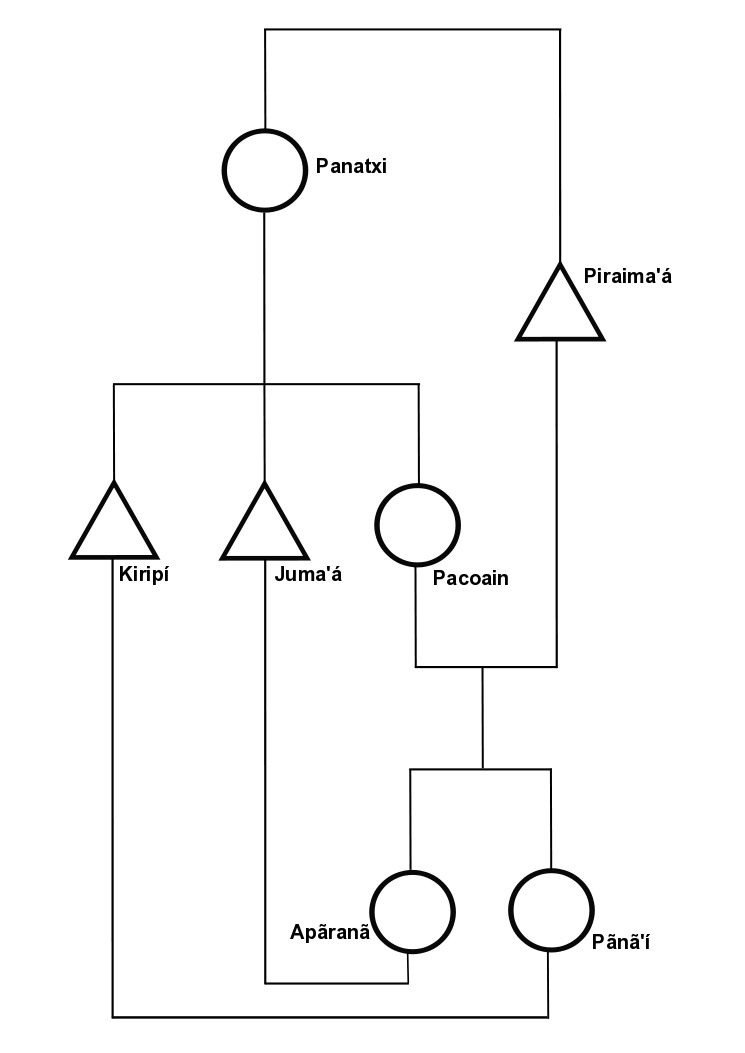
\includegraphics[width=.5\textwidth]{./imgs/Figura_9}
% %\caption{Figura 9}
% \end{figure}

Pira'ima'ã tem planos de enviar, \textit{mãj manã}, sua filha Panỹ'ia,
assim que estiver crescidinha, para viver com Kiripia (\textsc{mb}), e a
distância etária entre os dois é de 10 anos. Nesse caso, aconteceu o
oposto do que ocorreu com Juma'ã, irmão de Kiripia, que hoje vive em uma
casa anexa à de Pira'ima'ã, em um esquema --- chamemos assim --- uxorilocal.
Pira'ima'ã disse que não liberaria sua primeira filha para sair de casa;
enquanto a segunda ele prefere que vá viver na casa do marido.\footnote{Virilocalidade.} 
Isso mostra quanto a aliança Guajá não está preocupada
com a residência, e cada caso deve ser observado em particular. Notemos
ainda que no caso acima não me refiro a pessoas adultas; ao contrário,
as futuras-esposas a que me refiro (Panỹ'ia e Aparanỹa) encontram-se
ainda na infância, enquanto os maridos (Kiripia e Juma'ã) são meninos
muito jovens. Para o caso das esposas, como ainda veremos abaixo, a
idade precoce é condição para o casamento.\footnote{Como outro exemplo,
  no caso dos Cinta Larga, mesmo que a idade de casamento definida seja
  entre sete e dez anos, muitas vezes um dos irmãos da mãe (o noivo
  diretamente interessado) faz o pedido de casamento logo que a menina
  nasce --- ou antes da idade de sete anos --- comprometendo-a. O pai, por
  sua vez, não pode recusar o pedido, uma vez que o risco de feitiço
  contra a criança, por parte do solicitante enraivecido, não é
  descartado nesses casos. Trata-se assim, segundo Dal Poz, de uma
  ``dádiva compulsória'' (Dal Poz, \textit{op.\,cit.}, p.\,113). Em qualquer outro
  pedido que venha para a mesma menina, o pai dela se desculpa ``dizendo
  que a menina já está prometida''. É importante dizer que, nesse
  caso, a jovem esposa terá suas atividades infantis salvaguardadas na
  nova casa ou grupo do marido, ela brinca com os pequeninos de sua
  idade durante alguns anos e só assume suas atividades de esposa,
  propriamente (cozinhar, colher, tecer), bem como as relações sexuais
  após a primeira menstruação (Dal Poz, \textit{op.\,cit.}, p.\,114). Na língua cinta
  larga, os casamentos são literalmente pagos, e para casar diz-se
  \textit{asaj'ã} --- ``pegar cônjuge''. O pagamento muitas vezes é feito
  com flechas, redes, espingardas, roupas, munição.}

Muitas são as formas de um homem se aproximar de uma mulher. Por
exemplo, o jovem Ki'ipia, filho de Takwarẽxa'a, que há poucos anos era
considerado um \textit{mihua}, apesar de ser solteiro flerta com algumas
mulheres da aldeia e com uma delas mantém relações sexuais tal como um
esposo --- é considerado ``marido'' de uma delas. Isto se deve graças ao
fato de trabalhar para diversas famílias da aldeia. No caso de Ki'ipia,
por enquanto o trabalho é sua única garantia de permanência na aldeia
além de, eventualmente, dormir com uma ou outra mulher casada. Em outro
exemplo, o jovem Juma'ã, embora trabalhe para seu sogro (e \textsc{mb}),
Pira'ima'ã, o faz com menos intensidade que Ki'ipia --- que chegou na
aldeia Juriti sem relação qualquer. Juma'ã, além de ser sobrinho (\textsc{zs})
de seu sogro e trabalhar para ele, tem liberdade para fugir do trabalho
e lhe negar ajuda; essa liberdade Ki'ipia, por ser um completo estranho,
nunca terá.

\section{casamentos, separações e outros afetos}

Após a morte de seu esposo, uma mulher se casará novamente. Em tais
ocasiões, apesar da possibilidade de levirato, outros homens --- próximos
ou não --- podem vir a desposar a viúva que, nesse caso, tem autonomia
para escolher seu novo marido. O rapto de mulheres, forma usual de
obtenção de esposas entre os Tupi orientais,\footnote{Ver Fausto, 2001.} são
narrados como eventos de ``antigamente'', embora, como vimos no capítulo
anterior, a possibilidade de contrair casamento por raptos é presente
quando o assunto são os \textit{mihua}, os atuais isolados. A troca de
esposas também é comum, principalmente onde há uma oferta grande de
mulheres desposáveis, como na aldeia Tiracambu. Os Guajá casam-se
algumas vezes durante a vida, e as separações são frequentes. É comum
moças jovens que largam homens velhos com quem estavam casadas,
sobretudo hoje, quando preferem rapazes jovens. Um homem, ao se casar
novamente com uma menina jovem, muitas vezes dispensa a primeira esposa,
que pode se casar com um rapaz mais jovem ou ainda lutar pela atenção do
marido, disputando com a coesposa um papel de destaque. Para uma mulher
dispensar um marido não precisa de muito, a primeira coisa que ela fará,
além de brigar, é colocar defeito em tudo que o homem faz. Tatuxa'a já
era casado com Parapijỹa e conta que sua segunda mulher, Pitõna, nunca
havia gostado muito dele, mas sim de Tamata, um jovem da aldeia
Awá com idade próxima à dela (Tamata tinha 23, Pitõna 18 anos e
Tatuxa'a, 33). Nesta época (entre 2009 e 2011), Tatuxa'a estava casado
com as duas e sempre se lembrava de quanto era difícil ter duas esposas,
pois o homem deve caçar e trabalhar muito para sustentá-las. Pitõna
ainda era bem novinha e, segundo Tatuxa'a, já se encontrava às
escondidas com Tamata. Certo dia, Tatuxa'a voltou de uma produtiva
pescaria e, como fazem todos os homens da aldeia (mesmo com as meninas
mais novas), pediu a Pitõna que limpasse os peixes para, em seguida,
cozinharem um caldo --- \textit{pira tekwera}, ``caldo de peixe'' --- a ser
consumido com farinha. Pitõna estava acostumada a fazer o trabalho,
antes para seu pai e agora para Tatuxa'a, mas dessa vez eis que ela,
muito brava, respondeu a seu marido: ``--- O que foi, agora você é
aleijado, não tem braço não? Não tem mão?''. Desconcertado, Tatuxa'a teve
que chamar sua outra mulher, Parapijỹa, --- \textit{hamirikopya}, ``primeira
esposa'' --- para fazê-lo, já que sua ``esposa recente'', \textit{hamirikopuhua}, 
não mais o tolerava. Por fim, Tatuxa'a foi para
um encontro em Brasília em 2011 e quando retornou à aldeia Pitõna já
estava vivendo com Tamata.

Apesar de eu fazer usos aqui de expressões como a mulher foi ``pega'',
``dada'', ``oferecida'' e outras herdadas da nomenclatura da teoria da
aliança da antropologia, uma ideia recorrente entre os Guajá defende que
a esposa \textit{escolhe} o marido. Além disso, quando há interferência
dos pais, costuma ser a mãe (e não o pai) da jovem que \textit{escolherá}
o marido da filha. Em diversos casos como no relato acima, como num
próximo que veremos mais abaixo e até mesmo como aquele com o qual abri
esse capítulo, mulheres insatisfeitas no casamento simplesmente não
permanecem casadas e, como já vimos, muitos outros homens já ficaram
infelizes por terem sido deixados. \textit{Imena ty}, ``largar o marido'',
assim como \textit{hamiriko ty}, ``largar a esposa'', em oposição a
\textit{imena pyhy}, ``pegar um marido'' e \textit{hamiriko pyhy,} ``pegar
uma esposa'', são ideias elaboradas pelas pessoas da aldeia, e de muitas
maneiras, no sistema de aliança Guajá ``pegar'' e ``largar'' não são
categorias arbitrárias trazidas em minha análise, mas traduções
operativas para pensar os casamentos.

O ciúme e a disputa também apimentam as relações, a vida conjugal das
pessoas pode ser bem variada. Assim, um homem casado com duas ou mais
mulheres pode não querer abrir mão de sua (às vezes nem tão) velha e
primeira companheira, e pode também acumular até quatro ou mais
mulheres; esposas abandonam seus maridos para ficar com homens de que
gostem mais; uma mulher mais velha que tenha sido desprezada pelo marido
pode --- depois de reconquistá-lo --- voltar para casa e manter como amante
um jovem rapaz (que tenha se aproximado naquele período fora de casa) ou
mesmo levá-lo como um segundo marido, à revelia do outro; relações
extraconjugais podem ser aceitas entre irmãos que dividem a mesma
parceira --- dentre tantas outras possibilidades. Homens e mulheres mantêm
relações extraconjugais sem grandes problemas, embora (como tudo o que
fazem os Guajá) com bastante discrição, apesar de nem sempre as coisas
acabarem bem. O finado Marajaxa'a,\footnote{Nome fictício.} por exemplo,
tinha uma cicatriz nas costas por uma facada que levou de Pakawa'ĩa,
assim que ela chegou para viver com sua família na aldeia Juriti. Ele
quis tomá-la à força, ela não aceitou, resistiu e o esfaqueou. Enquanto
esteve vivo, as pessoas zombavam dele por isso.

Em todas essas situações, são acionadas as ideias de ``primeira esposa''
ou ``primeiro marido'', --- \textit{hamirikopya} ou \textit{imenapya},
respectivamente --- em oposição a ``esposa recente'' ou ``marido recente''
--- \textit{hamirikpuhua} ou \textit{imenapuhua}, respectivamente. Eu mesmo só
pude conversar sobre isso pela primeira vez muito recentemente, quando,
recém-separado do meu primeiro casamento, em 2014, ao retornar às
aldeias com a notícia de minha separação, algumas pessoas me
questionaram: \textit{mõ nirimirikopuhua mõ}? ``e onde está sua
nova esposa?'', todos queriam saber (e me perguntavam como estavam meus
filhos, pedindo para ver as fotos e ouvir as histórias, como de
habitual, em nossos reencontros). Nesse momento pude perceber que --- além
do fato de as pessoas \textit{awa} não se separarem para ficar sozinhas,
tal a noção individualista tão valorizada em nosso mundo --- aquilo que eu
via como casamentos e separações, poligamias e poliandrias, dentre
outras explicações que nós antropólogos ensaiamos para dar conta de
sistemas e valores outros --- de parentesco e aliança ---, era aqui
encarnado por uma distinção terminológica fundamental, que marcava
diferentes tipos de cônjuges (antigos e recentes, cada qual com suas
características) no processo de aliança Guajá. Abaixo apresento um
exemplo ocorrido na aldeia Tiracambu que ilustra com precisão os enlaces
e desenlaces de um casamento com maridos e mulheres, antigos e recentes.

Durante mais de 10 anos Akamatỹa e Maxikua foram casados. Passados esses
anos, em 2007 Akamatỹa casou com mais duas mulheres, Pinawaxika e
Manimya, irmãs entre si, e assim ficou com três mulheres. Akamatỹa teve
filhos com todas elas, e a relação entre ele e as duas irmãs era muito
boa; em contraposição à relação dele com Maxikua, que foi descartada do
casamento, teve que se mudar e passou a viver sozinha em uma casa que
estava vaga na aldeia Tiracambu. Alguns meses depois, Maxikua ainda
queria voltar a viver com seu antigo marido que, a esta altura, só tinha
olhos para as duas jovens irmãs (caçando, inclusive, para a mãe delas).
De forma estratégica, ela convenceu Pinawaxika, uma das irmãs e
coesposa, a ajudá-la na reconquista. E funcionou. Certo dia, os três
saíram para caçar e, em dado momento, Pinawaxika permaneceu para trás em
uma clareira a cuidar do filho, permitindo que Maxikua e Akamatỹa
avançassem floresta adentro, com o pretexto de ``matarem uma cotia'' e se
entendessem melhor. A partir daí eles se reconciliaram, e Maxikua, que
estava separada, voltou para Akamatỹa. Conclusão: Maxikua vive junto de
Akamatỹa, dividindo-o com suas outras esposas que, hoje em dia, são
quatro, pois em 2008 ele \textit{pegou} uma quarta --- e jovem --- esposa para
criar. Pinawaxika, por sua vez, se enamorou, \textit{maparỹ}, de Terexũa,
um rapaz mais jovem que ela, e até a última vez em que estive nesta
aldeia, 2014, dividia a vida entre os dois cônjuges: Akamatỹa e Terexũa.
É importante ressaltar que nas aldeias onde a oferta de casamentos é
maior (como a aldeia Tiracambu, no exemplo acima) os divórcios e
rearranjos conjugais também são mais recorrentes.

Por outro lado, muitas podem ser as formas de aproximação de um
pretendente com sua esposa. Na aldeia Juriti encontramos casamentos de
homens muito mais velhos com meninas muito jovens, como também de jovens
``tios'' (\textsc{mb}) com sobrinhas não tão mais novas assim. Um exemplo é o
último arranjo feito entre um rapaz de 13 anos, Juma'ã, e uma menina de
sete, Aparanỹa, \textsc{mb} e \textsc{zd} respectivamente. A irmã desse rapaz, Pakwa'ĩa,
mãe de sua (futura) esposa, mora em uma casa com seu marido e suas duas
filhas. Juma'ã mora em outra casa, fora do espaço da aldeia (embora
muito próximo), com seu grupo familiar: os mesmos pai e mãe de Pakwa'ĩa.
Certa ocasião, Juma'ã, embora muito jovem, passou a frequentar a aldeia,
levando sempre alimentos para a casa de sua irmã (\textsc{z}) casada com seu
sogro, seu \textit{hawaja}. Pira'ima'ã, o sogro, explicou-me que o jovem
pediu para ir morar com ele, pois estava querendo casar com sua filha. A
partir daí, passou a acompanhá-lo nas caçadas e ajudá-los em diversas
atividades cotidianas. Pira'ima'ã está, inclusive, construindo uma nova
casa, a fim de receber o \textit{hawaja}, seu afim próximo.

Assim como um jovem ``tio'' (\textsc{mb}) pode se casar com sua sobrinha, um
homem mais velho pode também desposar sua sobrinha jovem (\textsc{zd}), e não é
difícil haver diferenças de idade de 50 anos ou mais. E tanto os homens
quanto mulheres podem ser casados com mais de uma pessoa. Quanto a essa
poligamia, Cormier afirma que, na reserva Caru, onde realizou sua
pesquisa, a poliginia é mais comum, ao passo que a poliandria seria uma
experiência provisória. A autora defende que os padrões de casamento são
diferentes para homens e mulheres, devido à obliquidade em muitas
relações. Se tomarmos a aldeia Juriti como exemplo, de 11 casamentos
observados, três apresentam uma diferença etária de mais de 25 anos, um,
em mais de 10 anos, e quatro deles, entre 5 e 10 anos. Vejamos as
diferenças de idade em alguns deles baseadas nos dados etários
fornecidos pela \textsc{sesai}. Entre parênteses encontra-se a idade aproximada
do indivíduo.

\begin{table}[H]
\small
\centering
%\caption{My caption}
\label{my-label}
\begin{tabular}{|l|l|l|l|}
\hline
\textbf{\begin{tabular}[c]{@{}l@{}}Casamento\end{tabular}} & \textbf{Mulher}        & \textbf{Homem}       & \textbf{\begin{tabular}[c]{@{}l@{}}Diferença \end{tabular}} \\ [.5pt]
\hline\hline
\textbf{1}                                                      & Panypinuhũ (15)   & Pirama’ã (67)    & 52 anos                                                               \\ \hline
\textbf{2}                                                      & Hakwa'ĩa (28)     & Takwarẽxa'a (67) & 33 anos                                                               \\ \hline
\textbf{3}                                                      & Aparanaĩa (7)     & Pinawaxa'a (36)  & 29 anos                                                               \\ \hline
\textbf{4}                                                      & Amỹ Pirawãja (62) & Takya (49)       & 13 anos                                                               \\ \hline
\textbf{5}                                                      & Panyxĩa (37)      & Kamara (48)      & 9 anos                                                                \\ \hline
\textbf{6}                                                      & Ajruhua (37)      & Wirahoa (29)     & 8 anos                                                                \\ \hline
\textbf{7}                                                      & Aparanỹa (6)      & Juma'ã (13)      & 7 anos                                                                \\ \hline
\textbf{8}                                                      & Pakwa'ĩa (22)     & Pira'ima'ã (27)  & 5 anos                                                                \\ \hline
\textbf{9}                                                      & Amỹ Pirawãja (62) & Muturuhũam (66)  & 4 anos                                                                \\ \hline
\textbf{10}                                                     & Panyxĩa (18)      & Hajmakoma'ã (21) & 3 anos                                                                \\ \hline
\textbf{11}                                                     & Amỹ Pirahỹa (31)  & Uriximatỹa (28)  & 3 anos                                                                \\ \hline
\end{tabular}
\end{table}

Há ainda três casamentos que não estão na tabela, constituídos por
diferenças etárias menores do que três anos. Na tabela acima, os
casamentos ``4'', ``6'' e ``11'' são caracterizados por uma esposa mais
velha que o marido, sugerindo que a mulher dessa relação já fora casada
com outro homem, mais velho do que ela, já falecido, ou velho demais
para se manter como esposo. Não é difícil que um homem de uma ou mais
gerações ascendentes se case com uma jovem de uma geração descendente.
As diferenças de idade, como se pode ver, também são bastante variadas.
Muitos dos casamentos intergeracionais não são necessariamente
avunculares. Da lista acima, pelo que me consta, dos casamentos ``1'',
``2'' e ``3'', os de maior diferença de idade, somente o ``3'' é
avuncular. Os outros dois seriam ``somente'' intergeracionais. Pode haver
casos de casamentos com \textsc{zd} cuja diferença etária entre o tio e a
sobrinha é muito pouca. É o caso, na tabela, do casamento ``10''. Panyxĩa
(\textsc{zd}) e Hajmakoma'ã (\textsc{mb}) guardam uma diferença etária muito pequena, de
apenas três anos --- ele tem 21 anos; ela, 18. Assim, podem ocorrer
alianças marcadas pelo casamento avuncular em que a diferença etária é
pequena; ao passo que em outras, não necessariamente avunculares,
ocorrem casamentos intergeracionais. O casamento oblíquo e o casamento
intergeracional, no caso Guajá, não são necessariamente sinônimos,
embora possam aparecer juntos. Na tabela, os casamentos ``3'', ``7'', ``8'' e
``10'' são avunculares, e desses somente o ``3'' é baseado em uma diferença
etária considerável; os outros, mesmo que avunculares, guardam pouca
diferença de idade entre maridos e esposas.

Os Guajá, de muitas maneiras, gostam de arranjos que envolvam grandes
diferenças etárias e em que a preferência é por cônjuges de gerações
distantes, mas que podem ser desfeitos por qualquer um dos cônjuges. O
velho Xipowaha, de 54 anos, um dos fundadores da aldeia Awá (\textsc{ti}
Caru), era um segundo pai para o jovem Inamupihi'ũa, de 17 anos. Marido
de sua mãe, seria ele um \textit{tunewena} (\textsc{mh}) para o rapaz, como dizem
as pessoas desta aldeia. Xipowaha, há alguns anos, havia ``pego''
--- \textit{hamiriko pyhy}, ``pegar uma esposa'' --- para criar a jovem Tikwi'a,
hoje com 16 anos. Ela passava parte do tempo na casa de Xipowaha,
acompanhava as outras duas esposas em suas atividades, sendo ``criada''
por elas também, tal qual uma filha. Como Inamupihi'ũa também
frequentava essa casa, aos poucos ele e a jovem Tikwi'a, que são da
mesma geração, passaram a gostar um do outro --- \textit{maparỹ}, ``tomar
gosto'' --- e, antes que Xipowaha pudesse fazer qualquer coisa, os dois
jovens começaram a namorar, \textit{maparỹ}. A moça largou o homem que a
estava criando como esposa para se casar com o rapaz, que o marido
também chamava de ``filho'', \textit{haxa'a}. É como se Tikwi'a tivesse
sido ``pega'', \textit{pyhy}, ainda na infância justamente para ser ``criada'',
\textit{riku}, --- como se a conjugalidade fizesse as vezes de uma segunda
paternidade --- e quando decidiu escolher um marido de fato optou por
ficar com alguém que, em uma imagem mais ortodoxa, seria o ``filho do
marido''. O fato de Inamupihi'ũa e Tikwi'a decidirem ficar juntos também
passa por uma mudança radical (mas não só) que vem ocorrendo nas aldeias
do Pindaré (\textsc{ti} Caru), e me foi explicado que há uma recusa cada vez
maior dos jovens em se casar na condição de grandes distâncias etárias.
Isto seria coisa do passado, de ``antigamente'', \textit{imỹna}, no
limite, do ``tempo do mato'', \textit{imỹna} \textit{ka'ape}.

De acordo com Tatuxa'a, os homens, \textit{awatea}, se casavam com suas
\textit{hajnawãj mymyra}, literalmente, ``filhas das irmãs'', quando
viviam uma situação de menos densidade populacional. Tudo se passa como
se, na teoria guajá sobre o avunculato --- assim como em tantas outras
passagens da vida, como venho explicitando aqui ---, o casamento oblíquo
se justificasse apenas ``antigamente'', \textit{imỹna}, no ``tempo do mato'',
da mesma maneira que havia uma ``dieta de gente do mato'', \textit{awa
ka'apahara nimi'ũa}, e a vida em tapiris com suas aldeias do mato,
\textit{ka'a ripa}, ambas do passado. E o mesmo se aplicaria ao
parentesco. Quando viviam em pequenos coletivos, comendo animais que
hoje não mais consomem e dormindo em redes de tucum, casavam-se com suas
\textit{hajnawãj mymyra}, ``filhas das irmãs''. De acordo com essa
formulação, hoje eles não precisariam mais fazer isso e querem,
inclusive, moças de idades próximas. Não se trata aqui de associar o
avunculato ao passado, pois, como estamos vendo, muito da vida de
``antigamente'' ainda vigora na atualidade em diferentes situações,
sobretudo nas temporadas que experimentam em acampamentos na floresta,
ou mesmo em situações de contato com os brancos para
estabelecerem uma diferença entre ``eles'' e ``nós''. Trata-se,
diferentemente disso, de explicitar como os Guajá vêm pensando as
transformações de suas vidas em termos de sua própria história, cujas
mudanças, segundo eles mesmos, teriam implicações diretas inclusive no
sistema de aliança. Por outro lado, em muitas situações ao questionar
sobre casamentos de homens mais velhos com moças novas ou por que eles
se casavam com duas ou mais mulheres, diversos amigos respondiam coisas
do tipo ``é assim mesmo!'', \textit{a'e kĩa}, ou ``nós gostamos assim!''.

\section{casar}

Tal como estamos observando, os Guajá reservam pouca importância à
formalização de um casamento, isto é, não há mudanças radicais (mas sim
gradativas) e muito menos rituais que marquem tais passagens, tal como
também defende Taylor (2001) para o conjunto Jívaro e a maioria dos
grupos amazônicos. Quanto à coabitação, como já mencionado, mesmo
vivendo na casa de seus pais, a jovem noiva gradativamente se aproxima
do futuro cônjuge, tomando parte em suas atividades: 

\begin{enumerate}
\item Passa a acompanhá-lo em caçadas 
\item Deixa de tomar banho no rio de forma
animada com seus irmãos primos e amigos para acompanhá-lo nos banhos em
casal --- muitas vezes acompanhada de um irmão ainda de colo 
\item Passa a realizar suas refeições junto ao novo marido 
\item E, aos poucos, começa a frequentar sua rede. 
\end{enumerate}

Não há um momento específico para a moça sair da
casa de seus pais; e ela só toma essa atitude realmente um pouco antes
de engravidar e do nascimento do primeiro filho, o que atesta sua real
condição de esposa, \textit{haimirikoa}. A partir dos seis ou sete anos
de idade até sua gravidez, a menina experimenta uma gradual transição,
ao deixar de viver em sua casa natal para ficar ao lado do marido. O
casamento é visto como um processo gradativo de transformação de uma
menina em esposa e dessa esposa em mãe. Ela aprende neste processo a
``cantar bonito'' --- a principal marca de beleza e feminilidade que uma
mulher pode ter (aprende ouvindo sua mãe e irmãs); aprende a cuidar dos
filhos e a caçar com o marido ou na companhia de outras mulheres (pois
as mulheres Guajá também caçam). E o final da infância é o período da
descoberta do sexo (ao lado do marido e, muitas vezes, com alguns irmãos
dele, também chamados ``maridos'').

É dispensável mencionar que a ausência de marcas ou ritos de casamento
não implica uma perda na produção e instauração das relações
matrimoniais e afetivas e, muito menos, que elas sejam observadas como
algo secundário à vida das pessoas; ao contrário, talvez seja assunto
dos mais envolventes. Como já adiantei, os Guajá postulam que o
casamento é uma relação que pode ser ilustrada pelo verbo \textit{riku} ou
\textit{ruku}, cuja tradução mais conhecida é ``estar com''. Como ocorre em
outras línguas da família tupi-guarani, o verbo \textit{iku} é traduzível
por ``estar em pé em movimento'' (realizando alguma ação como: morar,
plantar etc.); no entanto, quando acrescido do prefixo
causativo-comitativo \textit{r}-, adquire a forma \textit{riku} e passa a
significar ``estar associado a algo ou alguém em movimento''.\footnote{Magalhães,
comunicação pessoal; ver também Magalhães, 2007.}\footnote{Foi Marcio
  Silva que me alertou para o fato de a tradução de \textit{riku}, tal
  como em outras línguas tupi, ser ``estar com'', noção que, como
  veremos, também faz referência ao \textit{riku} Guajá e é boa para
  pensar outras relações que ainda veremos. No entanto defendo que, para
  compreendermos o sistema de aliança enquanto baseado na relação
  \textit{riku}, a melhor tradução ainda é a que os Guajá me forneceram,
  isto é, ``criar''.} Em contextos específicos vários são os verbos do
português que podem ser utilizados para traduzir o \textit{riku} --- possuir,
casar, domesticar, amansar, criar, dentre outros ---, mas a tradução que
gostam de fornecer é ``criar''. Por isso, por uma questão de estilo e
efeito, utilizarei o verbo ``criar'', sabendo contudo que tal glosa pode
não ser necessariamente a melhor. Porém, ao traduzirem tal verbo como
``criar'' --- e não ``casar'' ou ``estar associado a'' --- indicam menos uma falta
de compreensão sobre o nosso léxico do que a sinalização para outro
sistema de ação, outra teoria sobre a relação conjugal, como veremos
agora.

\section{o verbo e o ato\ldots{} criando cônjuges}

Entre os Guajá não ocorrem ritos de iniciação, masculino ou
feminino, como entre seus vizinhos Tupi-Guarani: seja na \textit{Festa da
menina moça}, a \textit{Festa do moqueado} dos Guajajara, como pude
saber por intermédio dos próprios Tenetehara, em Santa Inês;\footnote{Ver também
Wagley e Galvão, \textit{op.\,cit.}} seja na reclusão da jovem Kaapor, quando de
sua primeira menstruação, marcando a passagem da menina à idade adulta.\footnote{Ver Huxley, \textit{op.\,cit.}} 
Quando uma jovem se casa, muitas vezes ainda em
idade precoce, inicia-se um ciclo cujo objetivo principal é transformar
a menina em uma esposa. Tal ciclo não compromete a vida em infância da
pequena esposa, que permanece desempenhando suas atividades corriqueiras
de criança: brincar, fazer bagunça, comer muito e, nas horas vagas,
acompanhar os pais em atividades de caça, roça ou coleta de frutos. O
casamento, muitas vezes, é uma relação que compreende diferenças etárias
que envolvem mais de um dígito, sendo muito comum uma mulher ser
proposta em casamento ainda na infância, e isso pode ser observado em
grande parte da bibliografia sobre a Amazônia, principalmente entre os
povos que prescrevem o casamento oblíquo.

Eis aqui um exemplo da aldeia Juriti. Até o ano de 2009, antes de seu
falecimento, Pinawãxa'a, então com 36 anos, estava casado com
Aparana'ia, de sete anos, filha de Amỹ Pirahỹa. Ele, irmão
classificatório de Amỹ Pirahỹa, se casou com sua sobrinha cruzada (\textsc{zd}).
No ano de 2006, em uma rápida visita que fiz à aldeia Juriti, quando vi
Aparana'ia pela primeira vez ela e seu marido ainda não estavam
``prometidos''. No ano seguinte (2007), quando retornei à aldeia para
iniciar a pesquisa de campo, eles já estavam juntos, e Pinawãxa'a dizia
ser ela sua \textit{hamirikoa}. Mas o que de fato mudara na vida de
Pinawãxa'a e Aparana'ia?

Superficialmente, pouca coisa havia mudado: a menina ainda passava o dia
com as outras crianças, brincando nas capoeiras e florestas imediatas à
aldeia; ainda chorava pelos mesmos motivos infantis que uma criança
chora --- como uma palmada de um irmão ou parente mais velho, ou uma
queda mais brusca provocada no contexto de uma brincadeira; e não tinha
nenhuma responsabilidade especial por ser \textit{hamirikoa}, ``esposa'', de
seu tio (\textsc{mb}). Por outro lado, a jovem passava algumas horas do dia
deitada na rede com seu marido. Certa vez Pinawãxa'a veio se queixar, em
tom dramático, que por haver se casado com Aparana'ia estava precisando
caçar bastante, pois tinha que levar comida para sua esposa e para os
irmãos dela, seus cunhados (\textsc{zs}). Pois uma das principais ``queixas'' dos
caçadores, sempre, é que precisam caçar muito para aplacar a fome de
suas esposas e filhos. Na minha segunda estada, entre fevereiro e abril
de 2008, a menina já passava as noites dividindo a mesma rede com ele e
o acompanhava nas caçadas, tal como uma boa esposa deve fazer. A jovem
experimenta a transição entre ``menina'' e ``mulher'' ou ``esposa'' coabitando
com seu marido, desde então, o responsável direto por sua alimentação.

Cormier (2003) afirma que a transição da jovem para a casa de seu marido
é gradual, e a menina só se muda definitivamente após estar plenamente
segura; até lá, se alterna entre a rede de seu marido e a rede na casa
de sua mãe. Por outro lado, parece não haver somente uma forma de
prestação do marido para com o pai da noiva, pois diferentes são as
idades de um \textit{imena} e diferentes são suas capacidades econômicas.
Pinawãxa'a já era um homem adulto e fazia para a menina Aparana'ia as
vezes de esposo e provedor, caçando para ela, seus jovens cunhados e
irmã, sogra (seu sogro era falecido). A jovem estava sendo literalmente
``criada'' por ele e após menstruar, quando engravidasse, estaria plena
para desempenhar suas atividades de esposa e daí se transformar em mãe.
Naqueles anos, mantinha com seu tio (\textsc{mb}) uma relação típica do
avunculato Guajá, que envolve um elemento fronteiriço entre a afinidade
e a consanguinidade: cria-se e casa-se.

Não é necessário que a jovem vá viver prontamente com o marido, porém
muitas vezes a relação é tão familiar que ela estará junto dele em
diversos momentos, querendo ou não. Além disso é importante que ela
permaneça frequentando a rede do esposo, vá caçar junto com ele e o
obedeça como se obedece a um pai. Aparana'ia, por exemplo, é uma menina
animada, vivaz, que adora brincar com seus irmãos mais novos e em
companhia de outras crianças, mas que acompanhava seu marido em
praticamente todas as atividades. No ano de 2007, quando Aparana'ia
ainda dormia na casa de sua mãe, o quente verão era também a época de
cantoria na \textit{takaja}. Durante esse momento ritual o homem traz do
\textit{iwa}, o ``céu'', dentro de si, um ``calor'' terapêutico, \textit{iwa
raku}, ``quentura do céu'', para soprar em sua esposa e filhos, como
parte de uma terapia de cura. As mulheres ficam em volta da
\textit{takaja}, cantando para seus maridos, enquanto, alta noite, as
crianças dormem um sono profundo. Os filhos são passivamente pegos pelo
pai e soprados, sem sequer acordar, diferentemente das esposas, que
permanecem acordadas participando da cerimônia e esperando pelo sopro.
Nessas madrugadas de cantoria, quando os homens entravam em suas casas
para soprar seus filhos, Pinawãxa'a adentrava a casa de sua irmã para
soprar sua pequena esposa e, em algumas ocasiões, após soprá-la já de
madrugada, ele a acordava e requeria sua companhia junto à
\textit{takaja}, tal como devem fazer as outras mulheres adultas.

\begin{center}\adforn{68}\end{center}

Como já mencionei, verbos como ``pegar'', \textit{pyhy}, também são
utilizados como sinônimo para ``casar''. Os Guajá defendem que um homem
apanha, \textit{pyhy}, uma menina ainda criança e que, uma vez que é pega,
inicia-se o casamento, \textit{riku}. Também entre os ``avunculares''
Cinta Larga, a noiva é dada em casamento ainda na infância após uma
``fala cerimonial'', quando o pai da menina não deve recusar o pedido, sob
risco de a criança ser enfeitiçada por retaliação ao matrimônio
frustrado --- embora nem sempre o pai dê a filha ao primeiro que apareça
(Dal Poz, 2004, p.\,113). Nesses casos, a língua cinta larga denomina o
casamento como \textit{asaj'ã}, literalmente ``pegar cônjuge''.\footnote{\textit{Idem}.} Nas aldeias Awá e Tiracambu, onde a oferta de jovens desposáveis é
superior à da aldeia Juriti, elas são logo cedo pegas em casamento, como
se prometidas\footnote{A ideia de \textit{prometer em casamento}, ocidental demais, presumo, 
não tem aqui rendimento etnográfico.} a seus tios maternos, a outros
homens e mesmo a jovens, e normalmente quem decide pelo futuro conjugal
da filha é a mãe, e não o pai.

Certa vez, conversando com uma dessas mães, Amỹ Pirahỹa, a mãe de
Aparana'ia, sobre o fato de as pessoas, \textit{awa}, se casarem com
meninas muito novas, ela me disse que elas precisam comer muitos
capelães, \textit{waria}, para crescerem e serem boas esposas, e quem
fornece essa carne são os maridos. A relação entre a comida e a
constituição da mulher como esposa é fundamental. A comida é a caça,\footnote{\textit{Hama'a}, ``minha caça''.} e os capelães são animais epítomes --- não por serem os mais gostosos, embora muito apreciados, mas por serem os
mais caçados).\footnote{Tanto Cormier (2003) quanto Forline (1997)
  apresentam em seus trabalhos os altos índices de ingestão de carne de
  capelães (\textit{Alouatta} \textit{belzebul}), se
  comparados a qualquer outra caça.} Se porcos, \textit{xahoa}, e antas, 
  \textit{tapi'ira}, são, de certa maneira, \textit{ideais de caça}, graças
às altas taxas de gordura e abundância de carne, eles não são tão
fáceis de ser abatidos como os capelães. Estes vivem mais próximos às
aldeias do que os primeiros,\footnote{Embora em um trabalho recente na
  área de antropologia evolutiva Medeiros aponte para mudanças (2007).}
o que torna as carnes de animais maiores, como porcos, caititus e antas, mais
cobiçadas. A relação entre a comensalidade e o processo conjugal é
difundida na Amazônia, onde \textit{cônjuges são concebidos como se tornando
consubstanciais por via do sexo e da comensalidade} (Viveiros de Castro,
2002, p.\,418), e no caso Guajá, a relação \textit{riku} é operatriz nesse
processo de cognação.

De maneira geral, em nossas conversas me explicaram que casar com
mulheres ainda muito jovens ocorre por motivos variados, e embora o
\textit{gostar}, \textit{maparỹ}, seja alegado para justificar os
casamentos, outros motivos foram criados para justificar esse
\textit{gostar}. Uma teoria muito recorrente é a de que quando um homem
toma uma menina por esposa ela não ficará \textit{brava}, \textit{imahy},
pois sempre terá comida suficiente. Toda mulher quer se casar ainda
jovem, e nenhuma delas toleraria crescer sem a quantidade de carne
fornecida por um marido. Caso um homem demore a desposar uma jovem, ela
se acostumará com a comida de sua mãe, e não mais aceitará outra. Não
que os alimentos sejam diferentes, mas por que ela estará se dando para
alguém que, durante sua infância, nunca caçou para ela. Para os Guajá
isso é um grande disparate. Nesta lógica, a ideia de as mulheres
esperarem pelo casamento até a idade adulta não é producente pois, como
disseram, elas estariam em um estado de raiva, \textit{imahy}, tão grande,
por não terem quem caçasse para ela, que não aceitariam ninguém como
cônjuge. Desta forma, os argumentos são de diferentes naturezas e,
claro, todos complementares: alguns de ordem \textit{econômica}, pois o marido
deve caçar para alimentar a mulher; ou de ordem \textit{social}, uma vez que,
caso ela não seja \textit{criada}, será muito brava em sua fase adulta; e até
mesmo sexual, como veremos, pois o sexo precoce prepararia a
menina para o futuro que lhe espera como esposa. Porém, em geral,
simplesmente me diziam: \textit{Jaha} \textit{amaparỹ} \textit{harinawãj}
\textit{mymyra}, em outras palavras, ``eu gosto da filha da minha irmã''.

Sendo assim, a principal tarefa do homem nos anos de formação de sua
esposa é propiciar seu desenvolvimento físico. Isso só é possível pelo
fornecimento sistemático de carne a ela e a sua mãe --- muitas vezes,
sua irmã real, pois classificatórias, como vimos, todas
são ---, e, quando também crianças, a seus jovens cunhados. A comida é para
todos. Desta forma, o \textit{riku} também é literalmente ``dar comida'',
como muitas vezes me explicavam de que se tratava o casamento,
principalmente os que envolvem grandes diferenças etárias.

\section{doçura e amizade}

Outro aspecto presente nesses anos de formação das esposas se refere às
relações sexuais.\footnote{Pela riqueza de sutis
significados e pela complexidade etnográfica que o tema das relações sexuais demanda, este livro aborda
o tema apenas de maneira tangencial.} O sexo, mesmo aparecendo como ponto
central dos regimes de conjugalidade, é um tema que exige tratamento
etnográfico preciso e adequado, pois caso contrário facilmente nos
arriscamos a parecer descuidados com nossos interlocutores e,
consequentemente, pode-se gerar uma série de mal-entendidos. Assim,
discutirei de forma controlada alguns pontos factuais que visam a ajudar
nesta análise do \textit{riku}, ``casamento'', guajá.

É bom lembrar que os Guajá se mostravam muito interessados em saber das
formas e preferências sexuais dos \textit{karaia}, ao passo que, por
discrição, não me falavam tanto de seus próprios interesses sobre o
tema. Se boa parte do diálogo de minha pesquisa foi estabelecido sob um
fluxo que envolvia troca direta de perguntas e respostas: a cada
pergunta que eu dirigia a \textit{eles}, me faziam duas ou três sobre \textit{nós}, e
quando o assunto era sexo, só eu falava, e não tive como fugir dessa
condição de \textit{tradutor da sexualidade dos brancos}. Perguntavam-me
sobre questões que versavam desde a nossa relação sogro-genro, passavam
por sexo oral, prostituição, e chegavam até cirurgias de
cesariana,\footnote{Alguns me pediram que eu levasse fotos da cesariana
  de minha filha. Queriam saber não só o nome do médico (que eu,
  obviamente, sabia!), mas também o do anestesista, das enfermeiras e
  auxiliares (o que, para surpresa de todos, eu não sabia!).}
inseminação artificial e medicamento restaurador da função erétil, como
o \textit{viagra}. As informações eram recebidas com risadas e caretas.
Quando mencionei sobre o viagra, por exemplo, Hajmakoma'ã me lembrou que
as pessoas de sua aldeia conhecem um medicamento semelhante, chamado
\textit{watijua}, que faz o homem ter ereção.\footnote{\textit{Hajmõ hatỹ}, ``pênis
duro'', ``firme''.}

A jovem Aparana'ia, que na época de minha pesquisa estava com nove anos,
além de frequentar a rede de seu marido, Pinawãxa'a, tinha uma relação
bem próxima com Wirahoa, irmão de seu esposo (\textsc{hb}), que, como vimos na
terminologia, é também referido por \textit{imena}, marido. Wirahoa,
inclusive, não cansava de dizer que, mesmo comprometida com seu irmão,
Aparana'ia também era sua esposa.\footnote{\textit{Harimirikoa}, ``minha esposa''.}
Pinawãxa'a ainda informou que sua pequena esposa está sendo \textit{criada} por
ele e por sua irmã, e que quando sua irmã se casou seu cunhado (\textsc{zh})
disse que faria uma esposa para ele criar, mas que só a daria para ele
depois que nascessem os seios.\footnote{\textit{Ikamykỹa}, ``os seios dela''.} Se o
caso for esse, o de um casamento intergeracional, como o de Pinawãxa'a,
é muito comum a espera de muitos anos até que a esposa fique
\textit{parahỹ}, ``bela'', para casar. E se, de maneira incauta,
perguntarmos a algum homem quando começam a manter relações sexuais com
a jovem esposa, serão categóricos em afirmar que somente depois de os
seios aparecerem; isso marca, de maneira um tanto simbólica, o fim da
infância de uma jovem.

O jovem Juma'ã, à época com 14 anos, que iria se casar com Aparanỹa, de
oito anos, era constantemente zombado pelos amigos de mesma idade e
que não tinham esposa por, supostamente, manter relações sexuais com uma
menina tão nova, ao que negava enfaticamente, morrendo de vergonha
dessas brincadeiras. O pai da menina, Pira'ima'ã, costumava dizer que os
dois deveriam ficar juntos --- \textit{namorar}, ele disse em português ---, pois
Juma'ã já sabia caçar e podia pegar carne para a menina, e muitas vezes
ele os aconselhava a irem caçar somente os dois, nada muito longe, para
que ela ficasse junto, \textit{riku}, do rapaz. Era nessas situações que
seus jovens amigos, e até mesmo homens adultos, insinuavam que eles
faziam sexo.

O sexo é dito ser \textit{he'ẽ}, cuja tradução é ``doce'' ou ``gostoso'', da
mesma forma que o mel, \textit{haira}, é doce, em oposição ao
\textit{amargo}, \textit{irawahy}. Vários sabores agradáveis, além de
frutas e mel, como a gordura animal ou a farinha de macaxeira, \textit{makaxia},
mais leve que a de mandioca, são definidos pelos
Guajá como \textit{hee'ẽ}.\footnote{Este termo encontra cognatos em outras
  línguas tupi, como o \textit{-e'ẽ} Mbya (ver Dooley, \textit{op.\,cit.}), cuja
  tradução também é ``doce''.} Além do sexo, para um homem, as mulheres, e
principalmente suas vaginas,\footnote{\textit{Hamixa'ỹa} ou \textit{hajkwara},
``buraco dela''.} podem ser ditas \textit{he'ẽ}, sendo essa ideia a que
melhor define o sexo. Não por acaso, os méis doces, além de serem um
alimento saudável às emoções e à saúde mental,\footnote{Como vimos no capítulo
3.} carregam em si uma lascívia, justamente por serem extremamente
\textit{he'ẽ}, ``doces''. Quando os mais jovens me perguntavam o que era o ato
sexual, \textit{iminũ}, para mim, sempre perguntavam se eu achava as
vaginas realmente \textit{doces}, tal como eles.

O código do mel doce, \textit{haira} \textit{hee'ẽ}, e das relações sexuais,
\textit{iminũ}, além de outras sensações, parece fazer referência às
duas coisas, o que é atestado pelo fato de a maioria das entradas das
colmeias, \textit{xapira}, nas árvores serem referidas por pênis,
\textit{haimõa}, ou vagina, \textit{hamixa'ỹa}. Isso irá depender da
espécie de abelha. Cada uma dessas colmeias tem um formato de entrada
que pode ser chamada de ``boca'', \textit{irua}, ou ``nariz'',
\textit{japijawỹna}, ``vagina'', \textit{hamixa'ỹa}, ou ``pênis'', 
\textit{haimõa}, a depender da espécie.\footnote{Como exemplo, o orifício de
entrada das colmeias de uma abelha chamada \textit{haipiuna} é referido
como um \textit{haimõa}, ``pênis'', enquanto a entrada da colmeia das abelhas
\textit{jakaira} é designada um \textit{hamixa'ỹa}, ``vagina''.}

Lembro que a relação entre a doçura do mel e o sexo, tal como estamos
vendo entre os Guajá, já foi comentada para o caso amazônico em obras
importantes. Assim descreve Lévi-Strauss:

\begin{quote}
{[}\ldots{}{]} os méis das {[}abelhas{]} melíponas, cujos perfumes são muito
variados, mas sempre de uma riqueza e de uma complexidade indescritíveis
para quem não os experimentou, possuem sabores tão marcados que se
tornam quase intoleráveis. Um gozo mais delicioso do que qualquer um
daqueles proporcionados habitualmente pelo paladar e pelo odor perturba
os limiares da sensibilidade e confunde seus registros. Já não sabemos
mais se degustamos ou se ardemos de amor. Estes laivos eróticos não
passaram despercebidos do pensamento mítico.\footnote{Lévi-Strauss, 2004, p.\,46.}
\end{quote}

Em muitos mitos sul-americanos, o mel é carregado de um \textit{poder sedutor}
ligado a sua doçura, e erótico, se relacionado à imoderação com que muitas vezes é 
consumido (Lévi-Strauss, 2004 (1967), p.\,242).\footnote{Por ora, não tenho condições de fazer uma
  análise do poder sedutor do mel, relacionando-o às Mitológicas e aos
  desdobramentos que lá encontramos. Agora, só apontarei esse diálogo,
  que tenho a intenção de aprofundar em outro momento.} Cobiçado de
maneira um tanto desmedida, esse alimento também é, entre os Guajá,
ordenado pelo código sexual, e sua doçura, comparável à doçura do sexo.

\section{«a critique of the study of kinship»}

Dentre as sutilezas que o sexo envolve, a paternidade, tema central na
discussão dos sistemas de aliança e conjugalidade, também é tratada com
discrição entre pessoas. Em linhas gerais, por meio de seu esperma,
\textit{na'arera},\footnote{Minha etnografia carece de dados sobre a
  produção e concepção de substâncias como, por exemplo, o esperma. Como
  um paralelo, sugiro a leitura da elaborada descrição sobre o esperma
  em outro grupo Tupi-Guarani, os Waiãpi do Amapá, realizada por Rosalen
  (2005, pp.\,54--57).} outros homens ``ajudam'' a mulher durante a
gravidez, se tornando \textit{pais} da criança, tal, como sabemos, é
difundido na literatura etnológica amazônica.\footnote{Para um balanço
contemporâneo, ver Beckerman \& Valentine, 2002.} No caso Guajá, é comum
que alguém conte com dois e, eventualmente, três ou mais homens que
tenham participado da sua concepção. Além do irmão do pai (\textsc{fb}), que
mantém proximidade terminológica com a figura paterna (\textsc{f}), o sistema
Guajá também conta com outra relação de \textit{copaternidade}. Esse outro
\textit{pai} é chamado \textit{tunewẽna} e difere terminologicamente de \textsc{f},
classificado como \textit{tua,} e de \textsc{fb}, também pensado como ``pai'' a
partir da ideia de \textit{tunã}, ``parecido com pai''. O \textit{tunewẽna}
--- enfatizo, diferentemente de \textit{tua} (\textsc{f}) e \textit{tunã} (\textsc{fb}), irmãos
entre si --- é vinculado ao universo dos afins da mulher, quase sempre
distante da parentela próxima do casal. Para ego, o termo vocativo para
\textsc{f} e \textsc{fb} é ``pai'', \textit{xipa}, e esse mesmo termo, \textit{xipa}, é
utilizado em relação aos pais do tipo \textit{tunewẽna}. Trata-se de uma
figura que, pelo sexo com uma mulher, é transformado em uma espécie de
``pai biológico'' sendo, muitas vezes, um amigo próximo do marido desta
mulher que a tenha ajudado a engravidar. O \textit{tunewẽna} é aquele que
\textit{japo pamẽ}, explicou-me certa vez Irakatakoa, aquele que ``faz {[}o
filho{]} junto (misturado)''. Por sua vez, por ser tornado \textit{tunewẽna}
a partir desta ação sexual, \textit{tunã} (\textsc{fb}) e \textit{tunewẽna} podem ser
(e muitas vezes efetivamente são) a mesma pessoa. Suponho que isso fosse
mais comum antes do contato, no tempo de uma endogamia parcial dos
pequenos grupos locais --- quando, inclusive, o avunculato e a poliginia
sororal eram ainda mais frequentes ---, quando não existiam grandes
aglomerados (como hoje) e os ``parentes distantes'', \textit{hapihianỹ},
estavam espacialmente ``distantes''.\footnote{\textit{Mĩpe}, ``lá longe''.} Vejamos,
no entanto, um exemplo atual.

A aldeia Tiracambu contava com 59 pessoas em 2013. A partir de uma
pequena amostragem feita com 37 pessoas e que coletei de maneira
aleatória em conversas com alguns amigos da aldeia na época, deste
universo de 37 indivíduos, 18 eram lembrados por terem ao menos um outro
pai do tipo \textit{tunewẽna}, ``pai compartilhado''. Desses 18, 12
contavam com \textit{dois pais}, cinco com \textit{três pais} e um com \textit{quatro pais}. Lembro
também que essa correlação é pautada diretamente pelo grau de interesse
que os homens mantêm por uma mulher. Por exemplo, no caso da moça que
tem quatro pais (o marido de sua mãe (\textsc{f}), além de três \textit{tunewẽna}), sua mãe
(\textsc{m}) era considerada uma das mulheres mais atraentes pelos homens das
aldeias Tiracambu e Awá e, certamente, ela devia ser
bastante assediada pela \textit{rapaziada}.\footnote{\textit{Awa wanihãkera}, ``muitos
homens juntos''.}

Podemos dizer que, no contexto geral, uma criança pode contar com vários
\textit{tunewẽna}, porém tal posição de \textit{pai compartilhado} se vincula a
uma relação de \textit{amigos}, ou melhor, de um tipo de \textit{amigo} com
quem se divide a esposa, e encontra paralelos em outras etnografias.\footnote{Tal como na relação \textit{apĩhi-pihã} observada nos Araweté (Viveiros de
Castro, 1896, pp.\,422--437).} O que parece marcar o vínculo de um
\textit{tunewẽna} com ego ocorre na geração \textsc{g}+1, ou seja, é a relação de
amizade estabelecida entre os pais de ego (\textsc{f}, \textsc{m}) e outro homem, que
possibilitará a copaternidade. Tal relação entre dois homens é chamada
\textit{harapihianỹtea}, cuja tradução literal é ``meu afim de verdade'' ---
e uma boa tradução, além de ``amigo'' nesse sentido específico da
amizade amazônica, pode ser ``melhor afim''. Encontramos, portanto,
entre os Guajá um tipo muito particular de relação de \textit{amizade}, que aqui não seria \textit{formal}, 
tal como foi discutido em outras
paisagens amazônicas, cada qual com suas conotações.\footnote{Para outros casos
Tupi, ver Kracke, 1978, p.\,14; Wagley, 1977, pp.\,73--75; Grenand, 1982,
pp.\,138--141; além dos Jê discutidos por Da Matta, 1976, pp.\,138--154; Seeger,
1981, pp.\,142--145; Carneiro da Cunha, 1978, pp.\,74--94; 1979, \textit{apud} Viveiros de
Castro, 1986, pp.\,435--437; para uma releitura sobre o tema da amizade
formal Jê, ver Coelho de Souza, 2004; para casos etnográficos
específicos, ver Viveiros de Castro, 1986; Da Matta, 1976; Lea, 2012).}

Algo que me chamou atenção durante uma estadia na aldeia Tiracambu em
2013 foi o fato de uma mulher, já casada em uma aliança poligínica
sororal, ter levado um jovem rapaz para viver em sua casa junto a seu
então marido e a outra esposa. Onde antes viviam duas mulheres (irmãs
entre si, a mais velha {[}e\textsc{z}{]} com 29 e a mais nova {[}y\textsc{z}{]}\footnote{Irmãs
  \textit{mais velha} (e\textsc{z}) e \textit{mais nova} (y\textsc{z}), respectivamente.} com 24
anos), casadas com um homem de 52 anos, após anos de convivência e um
conjunto de cinco filhos (três de uma e dois de outra), passaram a viver dois
casais --- a mais jovem delas levou um rapaz com 17 anos para morar junto
deles. Pinawãxika (y\textsc{z}) disse a seu primeiro marido, Akamatỹa, que estava
``gostando'', \textit{maparỹ}, do rapaz e, com isso, Akamatỹa convidou-o a
morar em sua casa e ficarem com a mesma esposa.

% Verificar tabela
%\includegraphics[width=3.90694in,height=1.97014in]{media/image3.png}
% \begin{figure}[H]
% \centering
%   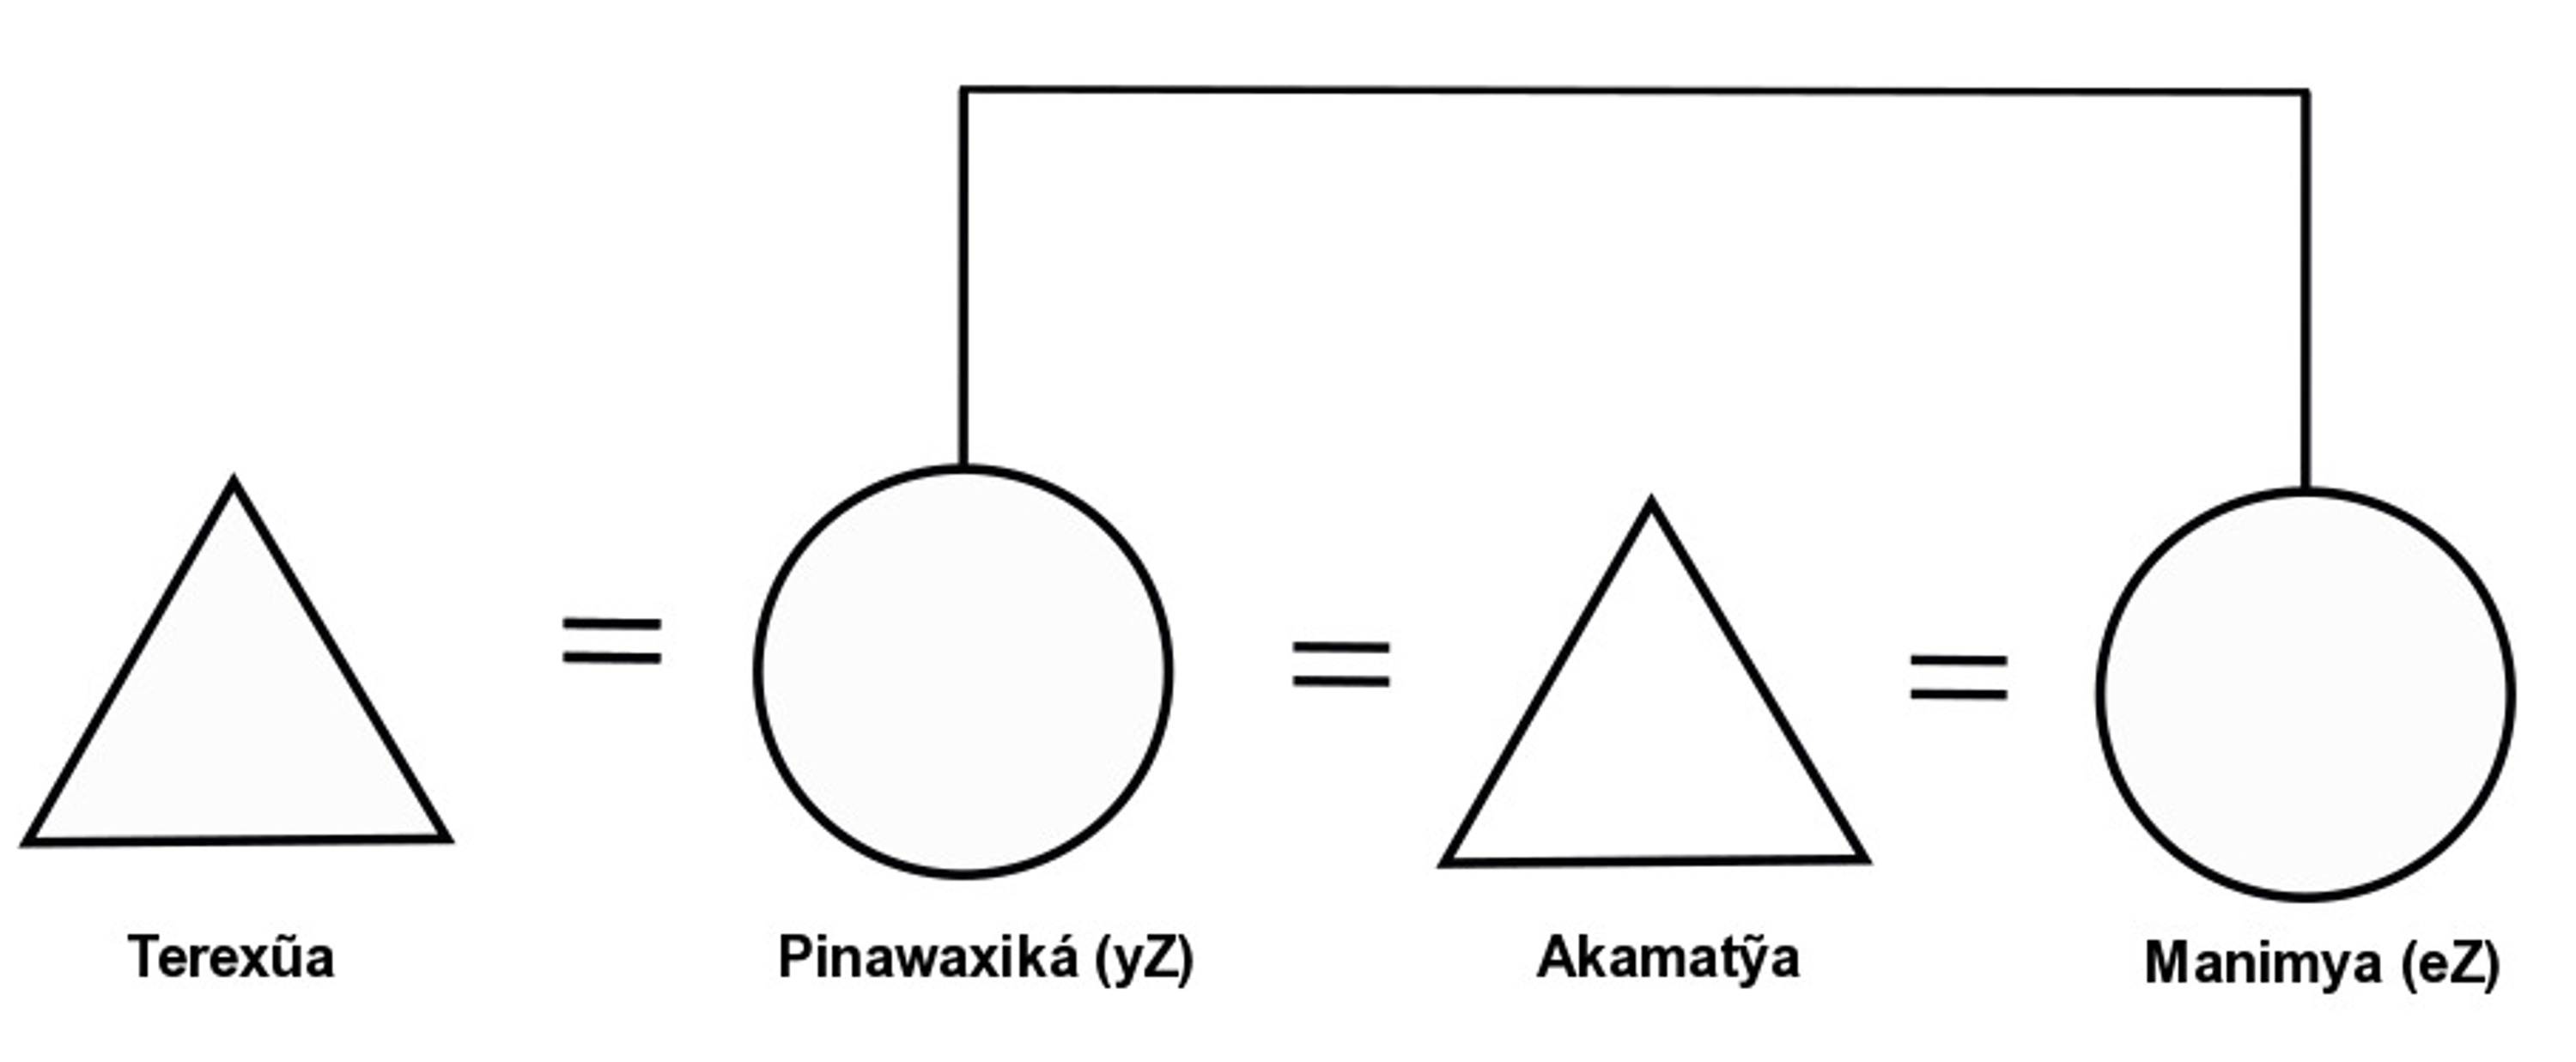
\includegraphics[width=.5\textwidth]{./imgs/Figura_10_crop}
% %\caption{Figura 10}
% \end{figure}

Ele recebeu o jovem tal como se recebe um \textit{filho} e passou a tratá-lo
como um \textit{harapihianỹtea}, ``afim muito bom'', um \textit{amigo} que,
nesse caso, pela grande diferença etária, era levado para caçar por
Akamatỹa. Ao jovem, o homem ensinava toda a arte da caça, além de
compartilhar com ele sua esposa mais jovem e, é claro, a paternidade dos
filhos. Akamatỹa e o jovem Terexũa, como se chama, agora são
\textit{harapihianỹtea}, ``melhores afins''. O rapaz já era \textit{tunewẽna},
``pai compartilhado'', do filho recém-nascido de Pinawãxika e Akamatỹa,
pois já vinha ``namorando-a'',\footnote{\textit{Maparỹ}, ``gostando''.} como um
amante, há alguns meses. Notem que o jovem Terexũa não compartilhava
qualquer laço cognático com nenhuma pessoa da casa e vinha de um pequeno
grupo contatado em local e época diferentes da maioria das pessoas da
aldeia. O pai de Terexũa, o falecido Hapaxa'a, era inclusive chamado de
\textit{mihua}, ``gente braba'', pelas pessoas da aldeia. Em outras
palavras, o parentesco que Akamatỹa dividia com Terexũa, se existisse,
era distante, nas \textit{bordas da afinidade} (Viveiros de Castro, 1986,
p.\,431), na periferia das relações reais, e eles foram aproximados,
transformados em cognatos, pelo casamento e procriação (Coelho de Souza,
2004, p.\,44). Este parceiro longínquo, filho de um \textit{mihua}, um
\textit{índio} \textit{brabo}, como traduzem os Guajá, avesso de um irmão
por ser um \textit{amigo}, cuja equivalência é algo a ser construído é 
a \textit{presa}\footnote{Viveiros de Castro, 1986, p.\,430.} ideal para
ser tornada esse tipo de \textit{amigo} --- alguém antes distante que agora
foi aproximado como um \textit{harapihianỹtea}, ``melhor afim'', por
meio do casamento.

Em outro exemplo, encontramos a mesma figura de \textit{melhor afim} também
sobreposta à figura de copaternidade, \textit{tunewẽna}. Pude encontrar nas
três aldeias onde trabalhei (Juriti, Tiracambu e Awá) duplas de
homens casados que levavam a vida juntos, lembrando inclusive, em muitos
aspectos, a relação \textit{apĩhi-pihã} Araweté: saíam para caçar
sozinhos; montavam acampamento de caça levando apenas as duas famílias;
dividiam o suprimento de munição e, hoje em dia, em algumas aldeias,
dividem o dinheiro para a compra de bens. Quando não dividiam a mesma
casa, eram vizinhos em uma mesma seção residencial. Warixa'a e Tatuxa'a,
que vivem na aldeia Awá, são desse tipo. Grandes amigos, ambos
são \textit{tunewẽna} dos filhos um do outro, compartilham o sexo com suas
mulheres e se pensam como \textit{harapihianỹtea}, ``amigos''; ``melhores
afins''. Da mesma forma, encontrei na mesma aldeia as duplas de
\textit{amigos} Takwarixika e Takwarixa'a e Majhuxa'a e Jamakwarera.
Enquanto Warixa'a e Tatuxa'a moravam em casas avizinhadas, as outras
duas duplas dividiam a mesma casa. Cada grupo de amigos vai conceber sua
relação de maneira muito particular e evoca motivos diferentes para
dizer por que estão juntos; em todos esses casos, persiste a ideia de
\textit{gostar desse jeito}, como me explicavam, para tantas coisas.

Como vimos acima, enquanto em alguns casos um homem solteiro é
transformado em \textit{amigo} dividindo uma esposa, em outros, dois homens
podem ser próximos desde a infância, como ocorre com Tatuxa'a e
Warixa'a. Ambos têm a mesma idade, aprenderam a caçar juntos quando
garotos, matando passarinhos, e por isso até hoje caçam juntos. E o
tratamento vocativo utilizados por esses \textit{melhores afins} é
\textit{hary}, que expressa a proximidade cognática. Do ponto de vista de
uma criança, o termo para esse ``pai compartilhado'' é \textit{tunewẽna},
enquanto uma ``mãe compartilhada'' será chamada de \textit{ihinewẽna}, que
difere de \textit{ihia} (\textsc{m}) e \textit{ihinã} (\textsc{mz}); da mesma forma que
\textit{tunewẽna} difere das figuras de \textit{tu} (\textsc{f}) e \textit{tunã} (\textsc{fb}).
Seriam eles algo como um \textit{terceiro} tipo de pais e mães, feitos a
partir da afinidade.

Como em diversos outros casos ameríndios, um bom critério para saber
quem são os \textit{pais} de uma criança recém-nascida, seus \textit{tunewẽna}
--- que, com exceções, costumam ser um ou dois, no máximo ---, é saber quem estará
observando o resguardo após este nascimento. A casca de árvore amarga,
\textit{mata'ya}, usada para proteger o fígado sensibilizado após o
nascimento de um filho,\footnote{Cf. capítulo 3.} é ingerida
pelo ``pais compartilhados'', \textit{tunewẽna}, pois o fígado deles se
torna vulnerável após o nascimento. Toda a \textit{couvade},\footnote{Cf. capítulo 3.} 
também deverá ser observada pelos \textit{tunewẽna}, sob o mesmo risco de adoecimento e morte dos
recém-nascidos. Podemos concluir com isso que, também para a
copaternidade, são seus efeitos que determinarão a figura dos pais. Nem
todo \textit{tunewẽna} será \textit{harapihianỹtea}, ``melhor afim'' ou
``melhor amigo'', e nem todo \textit{tunã} (\textsc{fb}) será \textit{tunewẽna}. Essas
posições oscilarão ao sabor dos afetos e das relações, porém se um homem
ajudou a fazer um filho em uma mulher, por ser \textit{tunewẽna}, sentirá
os efeitos da paternidade e deverá cuidar de si observando a
\textit{couvade}, o que demonstra, também aqui, um \textit{caráter
tentativo e experimental} das práticas de resguardo (Coelho de Souza,
2004, p.\,44). No caso Guajá, quanto menos participação um homem teve na
paternidade, menos relação manterá com a mulher ou com o casal, menos
proximidade e consubstancialidade terá com o recém-nascido e, portanto,
menos cuidado observará no resguardo. Em todo caso, cabe a cada
\textit{tunewẽna}, a depender das distâncias envolvidas nessas relações,
avaliar quanto o resguardo pós-nascimento deverá ser observado. Como
pontua Coelho de Souza, \textit{a consubstancialidade, em outras palavras, é
algo que se reconhece por seus efeitos} (2004, p.\,44).

Percebemos que os Guajá são bastante criativos em suas relações
conjugais. Porém, outro aspecto merecedor de destaque é que, se até
agora \textit{sexualidade} e \textit{parentalidade} --- o vínculo que
progenitores e/\,ou criadores estabelecem com a prole --- apareceram juntas
nesta análise, as possibilidades de ser \textit{pai} e \textit{mãe} no mundo guajá 
experimentam diferentes intensidades, onde nem
sempre o sexo entre homens e mulheres produzirá \textit{filhos}. Existem
casos em que casamentos produzirão mais casamentos. 

% Verificar tabela
% Como último exemplo,
% a fim de explicitar esta ideia, gostaria que observássemos o diagrama da
% família de Wirahoa no ano de 2015.

% \begin{figure}[H]
% \centering
%   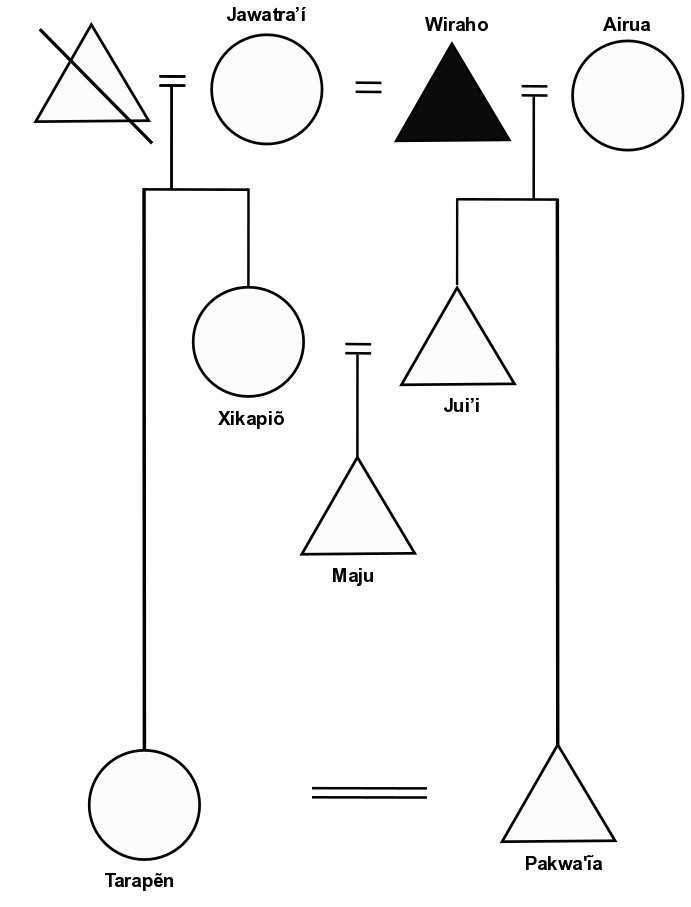
\includegraphics[width=.5\textwidth]{./imgs/Figura_11b}
% %\caption{Figura 11}
% \end{figure}

Wirahoa, de 38 anos\footnote{Coloco as idades correspondentes ao ano de 2015
como parâmetro.} casou-se com Ajrua, de 46, e desta
relação nasceram Juwi'ia, de 21, e Pakwa'i͂a, de 13. Passados 20 anos, o mesmo
Wirahoa se casou com a viúva Jawatara'ia, de 34, que chegou a esse
casamento com duas filhas de uma relação anterior, Xikapiõa, de 17, e
Tarapẽa, de 12. Um olhar desatento poderia pensar que Wirahoa se
transformaria em um \textit{pai} para as filhas de sua nova esposa, quando os
jovens virariam irmãos, mas na verdade o que ocorreu foi justamente o
contrário. Os quatro filhos já estão em idade de casar, e, com isso, a
jovem Xikapiõa se uniu a Juwi'ia em 2012, quando tiveram o pequeno
Majua. Atualmente, Pakwa'i͂a está ``namorando'', \textit{maparỹ}, a jovem
Tarapẽa, filha de Jawatara'ia, que já é uma mocinha.\footnote{Com
12 anos, as meninas começam a ter os primeiros filhos.} A futura
união de Tarapẽa poderá ser feita inclusive com um homem mais velho,
como já vimos em outros casos, mas, segundo as pessoas me disseram, os
dois jovenzinhos se gostam muito, \textit{maparyhỹ}, e já dividem a mesma
rede.

Para além de uma suposta endogamia de dois blocos familiares, observei
que, %(reparem no diagrama), 
de acordo com minha forma de apreender o
parentesco, ambas as \textit{avós} (\textit{paterna} {[}\textsc{fm}{]} e \textit{materna}
{[}\textsc{mm}{]}) eram casadas com o mesmo homem (Wirahoa), e, exagerando um
pouco mais, é como se o mesmo homem acumulasse a relação de avô paterno
e materno (\textsc{ff}, \textsc{mf}), uma vez que, vivendo com Jawatara'ia, Wirahoa
supostamente seria o novo pai de Xikapiõa. Mas nesse caso isso está
errado. Como sabemos de casos da aldeia Awá (Cormier, 2003, p.\,62),
um homem pode se casar também com a filha de sua esposa, na condição de,
obviamente, não ser sua própria filha. Cormier se refere a isso como
``\textit{Polygynous Wife's Daughter Marriage}'',\footnote{\textit{Idem}.} e o próprio
Wirahoa --- por que não? --- poderia ter desposado Jawatara'ia e Xikapiõa, que
são mãe e filha. Porém neste caso, não ele, mas seu próprio filho se
casou com a filha de sua mulher. Vemos no diagrama acima que o casamento
de Wirahoa com Jawatara'ia não produziu filhos ou irmãos entre si pelo
convívio, ao contrário, produziu mais casamentos.

A parentalidade se coloca como um problema de diferentes intensidades
que, a depender de como o sexo é administrado, poderá ou não estar
correlacionado.\footnote{Tal paradigma difere sobremaneira do parentesco
euro-americano, tal como nós o concebemos, em que sexo e parentalidade
são incompatíveis em toda sua extensão.} No caso da copaternidade,
\textit{tunewẽna}, discutida páginas acima, sexualidade e paternidade
aparecem como consequência uma da outra, quando amigos em comunhão,
\textit{melhores afins}, estão juntos na concepção da criança --- condição
muito diferente desta combinação de casamentos que vemos agora, em que
uma nova união ocorre e os cônjuges trazem filhos de situações
anteriores. Em outras palavras, para este último caso, \textit{no limite
da minha linguagem}, os termos aqui descritos poderiam aparecer de forma
negligente, simplificando a análise com as habituais ideias de \textit{pai},
\textit{mãe} e \textit{avôs} que, como sabemos,\footnote{Strathern, 2006 {[}1988{]}, 1995b;
1999b.} carregam sentidos muito próprios, capazes de comprometer a
análise. Meu exercício, portanto, está em contorcer, ou \textit{trair}, ao
máximo minhas próprias narrativas, pressupondo-se, por exemplo, que,
diferentemente do que é encontrado na classe média urbana brasileira,
na família de Wirahoa e nos Guajá de maneira mais geral, para casos em
que pessoas se casam com filhos de relações anteriores, as relações
sexuais podem estar completamente, ou em boa parte, desvinculadas da
parentalidade (\textit{parenthood}).\footnote{Como discute Marilyn
  Strathern, a comprovação da paternidade na sociedade ocidental está
  vinculada às relações sexuais do \textit{pai} com a \textit{mãe} (mesmo um
  padrasto deve tratar sua enteada \textit{como se} fosse uma filha), e o
  ato sexual, para nós, serve para produzir parentalidade (Strathern,
  1995b, p.\,307), que é o vínculo e legitimação de um casal enquanto pais
  frente a uma prole.}

De acordo com este argumento, correlacionar diretamente a sexualidade com
a parentalidade seria uma armadilha. O que nos põe na mesma direção da crítica de David
Schneider, ao perguntar o porquê de as unidades fundamentais do
parentesco serem, em todos os lugares, para a antropologia, relações
genealógicas. De maneira reflexiva, sua análise do parentesco americano
(1968) desvenda como nossas próprias concepções sobre o parentesco estão
por trás do pressuposto da universalidade da grade genealógica,
justamente porque nossa própria teoria sobre o parentesco é
simultaneamente uma teoria \textit{folk}\footnote{Popular e nativa.} da reprodução
biológica\footnote{Collier \& Yanagisako, 1987, pp.\,30--34.} Isso me faz perceber a
criatividade dos arranjos guajá como uma crítica à nossa maneira de
encarar a concepção de \textit{pais} e \textit{mães}. O fato de Wirahoa
manter relações com a \textit{mãe} de Xikapiõa, para os Guajá, em nada
transforma este homem em um \textit{pai} ou \textit{padrasto} para Xikapiõa. 
Ao contrário, é justamente porque um homem casou com
uma mulher que ele poderá se casar com a filha desta. Ele não a chamará
de \textit{filha}, tampouco ela o chamará de \textit{pai}. Podemos afirmar
que a produção e criação de filhos, preconizada pela percepção de
\textit{crescimento},\footnote{\textit{Ixa'a}, ``crescer''.} na qual a ideia de
\textit{riku} é também operativa, \textit{a priori}, não define homens e
mulheres como pais ou mães a partir do sexo no casamento, mas mediante um
convívio específico que mantenham com a prole.

\section{variações tupi: maridos e esposas}

Como mencionei mais acima, parece haver entre os Guajá uma preferência
pelo casamento intergeracional, que implica invariavelmente a ideia de
\textit{criação} como condição da própria relação conjugal. A aliança
avuncular e as grandes diferenças etárias podem aparecer juntas ou não.
Muitos casamentos entre \textsc{mb} e \textsc{zd} podem envolver homens velhos e meninas
púberes, mas o mesmo pode acontecer em um casamento entre duas pessoas
sem vínculos próximos. Por isso, se faz mister frisar que o casamento
avuncular e a escolha dos homens em desposar jovens meninas, embora
possam aparecer juntos, são fenômenos de natureza distinta, pois o tal
privilégio avuncular tende a ser respeitado, ainda que as idades sejam
próximas --- como salientei anteriormente.

A ideia de \textit{riku}, no entanto, não está indexada a diferenças
etárias, como se essas fossem um definidor da conjugalidade, sua forma
prototípica. Embora surpreendentemente a relação de \textit{criação}, de
filhos, xerimbabos ou esposas, possa pressupor a senhoridade, ou
maestria, em um polo da relação, tal como aparece também em diversos
contextos etnográficos --- sobretudo naqueles em que figuram alianças
oblíquas, quando a relação entre domesticação e casamento é
deliberadamente levada a cabo. Diversas análises, desde os antigos
Tupinambá\footnote{Fernandes Fernandes, 1963, pp.\,153--158.} até os Tupi
contemporâneos, pensam o processo de aliança a partir desse cenário de
\textit{criação} de maridos e esposas.

Sabemos que em diversas sociocosmologias sul-americanas, como
entre os Ashuar, Waiãpi, e até mesmo nos históricos Tupinambá, o
casamento é descrito como um processo de \textit{amansamento}, nas palavras de Anne
Christine Taylor, da esposa, muitas vezes desposada ainda bem jovem.\footnote{Entre os Guajá, a esposa 
é desposada por volta dos seis ou sete anos.} No caso
Ashuar, por exemplo, o casamento é modelado por uma relação de captura
violenta, já que, na prática, muitas esposas eram fruto de expedições
guerreiras entre diferentes grupos. O mesmo acontece com os Parakanã,
que davam preferência às jovens, \textit{pois as mais velhas eram difíceis de
pacificar} e, por vezes, resistiam à captura. Mesmo entre os Guajá,
quando mencionam os grupos que vivem sem contato com a Funai, uma das
principais preocupações dos homens é com as esposas de que os outros
poderão se apoderar, mesmo que seja por rapto, a partir do contato.

Para os Waiãpi, lembra Gallois, o \textit{apresamento} de mulheres é algo
tributário a um estado indômito das esposas e das mulheres em geral,
cuja captura e domesticação são necessárias a uma transformação da
jovem. No caso Guajá, tal necessidade é transformar uma jovem menina em
esposa. E as pessoas demonstram diversos motivos, de ordem econômica,
ecológica e sexual, para a preferência em se casar com um parente tão
próximo e tão jovem. Por fim, todos operam com a ideia de \textit{criar} a esposa, a
fim de que ela não entre em um estado de raiva incontrolável, destino a
que toda mulher está sujeita caso, por algum motivo, não se case.

Uma mulher não pode crescer sem estar casada, e não é recomendável que
ela demore para arranjar um marido, pois cresceria muito
\textit{zangada}.\footnote{Da mesma maneira que entre os Parakanã, ``o marido
  `cria' (\textit{pyro}) sua esposa pré-púbere dando caça para ela''
  (Fausto, 2001, p.\,432). Dar comida para a esposa (e para os sogros) é uma
  das principais atribuições do marido nesse período.} O que acontece
com a jovem esposa \textit{awatea} é algo parecido com o que Fausto
(2001, p.\,432) demonstra para as mulheres raptadas pelos Parakanã: uma
relação direta entre \textit{raiva}, \textit{comida} e \textit{casamento}, na qual o
alimento aplaca a raiva e possibilita o matrimônio. Como mencionei, os
Guajá têm diversas frases que ilustram o processo conjugal, como:
\textit{apyhy ta hamiriko nime,} ``vou pegá-la como esposa''; ou então:
\textit{amimakwa ta ha rehe}, literalmente, ``eu vou fazê-la acostumar-se
comigo''. O jovem Xiparẽxa'á, que estava gostando muito, \textit{maparỹ},
da jovem Majra, residente em outra aldeia, explicou-me que a ideia de
\textit{mimakwa}, ``amansar'', ``fazer acostumar-se a'', ilustraria o
\textit{namoro}, algo análogo ao ato de uma mulher trazer um filhote de cotia
do mato para criar. De acordo com Xiparẽxa'a, \textit{a cotia chega brava e tem
que ficar calma}. A fase de proximidade e conquista, \textit{maparỹ}, 
``gostar'', ou \textit{maparahỹ}, ``gostar muito'', é traduzida pela ideia
de amansamento, acostumar-se, \textit{mimakwa}, processo que pode durar
anos, e nem sempre quem ``amansa'' e ``cria'', \textit{riku}, será aquele que
terminará ``junto'', \textit{pyry}, com a mulher.

Esta máquina de produção de cônjuges, guardadas as devidas diferenças,
é, literalmente, operada por homens e mulheres. Mulheres trocam maridos
velhos por homens jovens, principalmente as mulheres jovens, como vimos
no início desse capítulo. Além disso, as mais velhas justificam o
casamento com homens de gerações inferiores argumentando que o marido
jovem \textit{caça mais} para elas. O \textit{riku}, como um modulador da
aliança, é aplicável para ambos os sexos: maridos criam esposas e
esposas criam maridos. Muitas mulheres viúvas que casaram novamente
dizem ``criar'', \textit{riku}, seus jovens maridos, pois o perigo, neste
caso, é o rapaz entrar em um profundo estado de melancolia por não
possuir uma esposa, capaz de comprometer inclusive sua produtividade na
caça: talvez o pior mal que se possa abater sobre um homem. Tal união,
com mulheres de gerações ascendentes, é característica não só dos
regimes avunculares, como sabemos desde os Tupinambá, mas também de
outros casos amazônicos. Em sua etnografia sobre os Asurini do Xingu,
que também se pensam \textit{awate,} ``gente de verdade'', Müller mostra
como as mulheres participam da \textit{formação da personalidade masculina}
pelo casamento intergeracional:

\begin{quote}
Aquele que eu criei, \textit{jeremymĩga}, tem este sentido, como termo de
referência usado pela esposa mais velha para o marido jovem. É frequente
ouvir as Asuriní comentarem que uma mulher mais velha, uma parente
próxima, deu, \textit{kae}, a elas o marido, a quem ajudou a formar. Ela o
ensina, contando mitos, histórias do passado {[}\ldots{}{]} Exige dele o
cumprimento das tarefas de roça e coleta para as quais ele está dando,
nesta fase de sua vida, a capacidade máxima do desempenho físico.\footnote{Müller,
1993, p.\,123.}
\end{quote}

No caso Guajá, as mulheres declaram literalmente \textit{jaha amixa'a ta
hamenime}, ``eu vou criá-lo para ser meu marido'', em que a ideia de
\textit{mixa'a}, ``fazer crescer'', denota o desenvolvimento físico de um
ser. As mulheres podem transmitir conhecimentos sobre como rastrear um
animal de caça, como me contou certa vez Wirahoa, ao relatar que sua
esposa mais velha ensinou-lhe a ``andar'', \textit{wata}, no mato, isto é,
caçar. Em suma, de um lado temos mulheres zangadas, e de outro, homens
melancólicos, ambos estados indesejados, e o enlace matrimonial é uma
das maneiras mais eficientes para os aplacar.

\section{a relação}

A partir da ideia de \textit{riku}, essa terminologia de relações variadas
atinge diferentes tipos de pessoas e seres, como veremos. No parentesco
isso ocorre ao ponto de o verbo determinar o próprio termo de referência
à ``esposa'', \textit{imiriko}. Sabemos que \textit{temericó} foi o termo
utilizado pelos Tupinambá seiscentistas para se referir a suas cônjuges
(Fernandes, \textit{op.\,cit.}, p.\,168), e se tomarmos as traduções linguísticas
usuais do \textit{reko} Tupi (como em Dooley, 1982), as ideias de ``ter'' e
``estar com'' justificariam a glosa do \textit{temericó} Tupinambá por
``aquela que eu tenho'' ou ``aquela que está comigo''. A raiz do termo
referente a ``esposa'' entre os Guajá é cognato ao \textit{temericó}
Tupinambá e se trata de \textit{imiriko}, ``esposa'', que em uma tradução
literal significa ``aquilo que está associado a''. Na língua guajá, o nome
para ``esposa'', \textit{imiriko}, aparece prefixado por marcas de pessoas,
ocorrendo nas forma a seguir, sob o seguinte paradigma:

\begin{itemize}
\item\textit{Harimirikoa}
``minha esposa''; ou, na tradução literal, ``aquela (ou aquilo) que está
associada/\,o a mim''
\item\textit{Nirimirikoa} ``tua esposa''; ou, ``aquela
(ou aquilo) que está associada/\,o a você''
\item\textit{Hamirikoa} ``a esposa dele''; ou, ``aquela
(ou aquilo) que está associada/\,o a ele''
\item\textit{Arerimirikoa} ``as nossas esposas'';
ou, ``aquelas (ou aquilo) que estão associadas/\,os a nós''
\item\textit{Pĩnimirikoa} ``as esposas de vocês'';
ou, ``aquela (ou aquilo) que está associada/\,o a vocês''
\item\textit{Wỹnimirikoa} ``as esposas deles''; ou,
``aquelas, (ou aquilo) que estão associadas/\,os a eles''\footnote{Agradeço
  a Marina Magalhães pela assessoria linguística neste tópico.}
\item\textit{Timirikoa} ``as esposas de alguém''; ou,
``aquela (ou aquilo) que está associada/\,o a alguém''
\end{itemize}

As formas acima são utilizadas a depender do contexto de enunciação, com
a raiz \textit{imiriko} mantida em todos os casos e que ressalta a ideia
de \textit{riku}. De acordo com Magalhães,\footnote{Comunicação pessoal.} a raiz nominal
\textit{imiriko} ainda pode ser subdividida linguisticamente em
\textit{{imi-r-iko}} $\rightarrow$ \textit{imi-} (prefixo nominalizador que transforma
verbos em nomes com função semântica de paciente, isto é, ``aquilo que
\ldots{}'') mais \textit{r-} (prefixo causativo-comitativo que transforma o verbo
\textit{iko} ``estar em movimento'' em ``estar em movimento associado a algo
ou alguém'') mais \textit{iko} (verbo, ``estar em movimento''). Desta forma,
uma tradução menos elegante para \textit{harimirikoa} é ``objeto do meu
criar'', tal como \textit{hanimi'ũa}, palavra cuja tradução é ``comida'',
deve ser traduzida por ``objeto do meu comer''. Outras traduções para
\textit{harimirikoa} podem ser: ``aquela a quem estou associado (ou
junto), produzindo uma \textit{ação}''; ou ainda, ``aquela que está
comigo sendo afetada por uma \textit{ação}''. A \textit{ação} em questão é o
próprio processo de aliança --- o \textit{riku}, o casamento --- formada por
diversas outras ações (comensalidade, sexo).

Desta forma, dado seu caráter agentivo, o \textit{riku} Guajá pode ser
pensado como um \textit{sistema de ação} que enfatiza \textit{agência,
intenção, causação, resultado e transformação}, tal a definição que Gell
(1998, p.\,6) empresta ao termo --- um \textit{sistema de ação} programado
para interferir (ou produzir) nas relações do mundo, e não um sistema
simbólico ou de atitudes, preenchido por regras, hábitos, prescrições e
preferências. O termo \textit{riku}, ele mesmo, é uma ``ideia de relação''
(que repercute o termo de Lima, 2005, p.\,94) formada por um conjunto de
ações tais que atravessam, ao menos a nossos olhos, diferentes ordens:
sexual, alimentar e xamânica --- esta última veremos no final do livro. A
tese que defendo aqui é relativamente simples, pois busca considerar o
``parentesco'' Guajá não pela forma que nossa tradição concebe as relações
de parentesco indígenas (ou qualquer outro sistema de ação não
ocidental,\footnote{``Não ocidental'' como uma ideia antropológica oposta a
  ``ocidental'', na acepção que lhe confere Ingold. Segundo o autor, o
  termo ``Ocidental'', na forma em que é utilizado pela antropologia,
  seria uma espécie de ``atalho'' (\textit{shorthand}) da linguagem
  científica, cuja principal característica (ou postulado) é a dicotomia
  entre natureza e cultura; humano e animal, dentre outras (Ingold,
  2000, pp.\,40--50).} como a ``arte indígena'', por exemplo),\footnote{Nas
  palavras de Gell: ``Eu vejo a arte como um sistema de ação, cuja
      intenção é interferir no mundo e não codificar proposições simbólicas
      a respeito dele. A `ação' --- como uma abordagem central para a arte --- é
      intrinsecamente mais antropológica do que a abordagem semiótica, mais
      preocupada com o papel mediador dos objetos de arte no processo
      social, do que com a interpretação dos objetos `como se' (\textit{as}
      \textit{if}) eles fossem textos'' (Gell, \textit{op.\,cit.}, p.\,6, tradução livre).}
mas por uma definição que leve em conta fundamentalmente uma teoria
Guajá sobre o processo de parentesco. A \textit{conjugalidade Guajá}, se
podemos assim denominar, faz referência a uma terminologia de relações
que ``transcende de muito a simples expressão de um laço de parentesco''
(nas palavras de Viveiros de Castro, 2002, a partir de Lévi-Strauss,
1943) e se liga a outras formas de socialidade, tal como encontramos em
outros contexto amazônicos. Vejamos melhor.

Na mitologia Waiãpi por exemplo, o apresamento de mulheres, presente em
diversas narrativas, é tributário ao estado indômito das esposas e
mulheres em geral:

\begin{quote}
O apresamento de mulheres, sua rebeldia e necessária domesticação me
parecem representar outro aspecto fundamental na concepção Waiãpi da
alteridade. Nas variantes do mito de origem dos inimigos, destacam-se
alguns comentários sobre as tentativas de domesticação dos inimigos.
Segundo a tradição, a maior parte desses povos foram inicialmente
'criados' pelos Waiãpi --- que pelo menos tentaram --- criá-los como seus
filhos. Diz-se \textit{o-nimo-bia} para ``criar e alimentar'' e
\textit{o-nimo-ry} para ``apaziguar, amansar, tratar com carinho, educar''.\footnote{Gallois, 1988, p.\,140.}
\end{quote}

Nesta concepção de aliança estão envolvidas a captura e a domesticação
(necessária, segundo a autora), cujo destino é a transformação. Que tipo
de transformação estaria em processo neste caso? Sob qual critério, além
do amansamento, alguém de fora, aqui uma mulher-esposa, é domesticada?
Pois para os Waiãpi, mas não só eles, o inimigo ou estrangeiro, mesmo
sendo diferente e repugnante, dentre outras classificações pejorativas,
é alguém ``afinizável'', e a guerra funciona como o oposto à domesticação.
Ela seria um processo de distanciamento, e ``praticamente todas as
versões do mito de origem dos inimigos ressaltam o fracasso da
domesticação, uma vez que, ao crescer, as criancinhas surgidas da
Anaconda manifestavam um gênio fundamentalmente agressivo''.\footnote{Ver
Gallois, \textit{op.\,cit.}, p.\,141.}

Se o casamento com a filha da irmã, como vimos, é um dos temas que
pontuam as análises da etnologia sul-americana desde seus primórdios --- e
diz muito sobre uma preferência presente em diversos povos em diferentes
épocas, desde o Brasil seiscentista até a Amazônia contemporânea ---,
vejamos outras formas de relação, caras também aos Guajá e presentes em
outros contextos etnográficos.

\section{entre humanos}

Recapitulando o que foi colocado até o momento --- pois esse conceito será
fundamental até o final deste livro ---, o verbo que exprime uma relação
conjugal é \textit{riku}, (ou, a depender da variante linguística do
falante, \textit{ruku}). Os Guajá, eles mesmos, traduzem para o português
como ``criar'', em uma metáfora vegetal do ``fazer crescer''. E, bem
entendido, não se trata de produzir algo novo, pois que para este caso
utilizam o verbo \textit{japo}, ``construir'', ``fazer''. Muito comum às
línguas tupi-guarani, os cognatos de \textit{riku} (como o \textit{reko}
dos Guarani) foram traduzidos de formas diferentes por linguistas e
antropólogos. Em seu ``Vocabulário do Guarani'' (Mbya), Dooley define
\textit{reko} como um verbo transitivo, cuja primeira tradução é ``Ter''.
Assim, ``\textit{Mba'e pa oguereko?}'' é traduzido por ``O que (ele) tem?''.
As outras quatro possibilidades de tradução, em Dooley, no entanto, se
referem a relações de domesticação e conjugalidade:
%, como vemos na tabela abaixo.

%\textbf{Traduções possíveis ao verbo \textit{reko}, em Guarani (Mbya)}%

%\begin{longtable}[]{@{}lll@{}}
%\toprule
%& \textbf{Tradução possível } & \textbf{Exemplos na fala}\tabularnewline
%\midrule
%\endhead
%1 & "Ter" & \textit{Mba'e pa ogue{reko}?} ➝ O que (ele)
%{tem}?\tabularnewline
%2 & "Criar (animais)" & \textit{eta ogue{reko} jagua ra'y} ➝ {cria} muitos
%cachorrinhos\tabularnewline
%3 & "Ter plantado" & \textit{a{reko}'i oro'u'i va'erã} ➝ tenho um
%pouquinho {plantado} para comermos\tabularnewline
%4 & "Conduzir (pessoa)" & \textit{xee ma torogue{reko} tape rupi} ➝
%deixe-me {conduzi-lo} pelo caminho\tabularnewline
%5 & "Andar junto com, ajudar (geralmente referindo-se a casados)" &
%\textit{peteĩ rami va'erã erereko xereindy} ➝ (você) vai {andar junto}, de
%acordo, com minha irmã.\tabularnewline
%\bottomrule
%\end{longtable}%

%(Fonte Dooley, 1982)

\begin{itemize}
\item \textbf{Ter}\quad \textit{Mba’e pa oguereko?}, ``o que {[}ele{]} tem?''
\item \textbf{Criar {[}animais{]}}\quad \textit{Eta oguereko jagua ra'y}, ``cria muitos cachorrinhos''
\item \textbf{Ter plantado}\quad \textit{Areko'i oro'u'i va'erã}, ``tenho um pouquinho plantado para comermos''
\item \textbf{Conduzir {[}pessoa{]}}\quad \textit{Xee ma toroguereko tape rupi}, ``deixe-me conduzi-lo pelo caminho''
\item \textbf{Andar junto com, ajudar {[}geralmente referido a casados}{]}\quad \textit{Peteĩ rami va'erã erereko xereindy}, ``{[}você{]} vai andar junto, de acordo, com minha irmã''
\end{itemize}

Além do fato de encontrarmos na linha dois a mesma tradução fornecida pelas
pessoas da aldeia Juriti para o verbo \textit{riku}, ``criar'', todas as
outras ideias também se encaixariam em outra tradução para o verbo
\textit{riku} --- essa, mais abrangente ---, fornecida por outra linguista:
``Estar associado, em movimento, a algo ou alguém''.\footnote{Magalhães,
comunicação pessoal.} Isto posto, ``criar'', ``plantar'', ``conduzir (uma pessoa)'',
``andar junto (à esposa ou ao marido)'', dentre outras definições que
podem, ou não, se conectar a essa, são passíveis de ser explicadas pela
ideia de \textit{riku}.

Quanto a uma ``tradução antropológica'', a ideia de \textit{riku} se
associa a esta forma generalizada de relação na Amazônia, que prescreve
relações assimétricas que gravitam em torno do conceito de ``donos''. De
um lado, mestres, donos, controladores --- e no caso Guajá, pais (\textsc{f}, \textsc{m}) e
cônjuges (\textsc{w}, \textsc{h}) --- e de outro, animais de caça, animais domésticos, mel
(e abelhas), frutos e vegetais --- e no caso Guajá, filhos e cônjuges, novamente. 
Abaixo, seguem exemplos:

\begin{enumerate}
\item A relação entre uma mãe e seus filhos é considerada uma relação do
tipo \textit{riku}
\item O laço conjugal estabelecido entre um marido e sua esposa é chamado
\textit{riku}
\item A relação perfilhada entre humanos e animais domésticos (chamados
\textit{nima}), filhotes de presas animais caçados e criados na aldeia, é
dita \textit{riku}
\item Da mesma forma, os objetos. Possuir uma flecha, uma faca, um tecido
ou qualquer outra coisa é manter com o objeto uma relação do tipo
\textit{riku}. No contexto guajá, a ideia de criar é mais significativa
para exprimir o controle do que o verbo \textit{possuir}. O portador de
determinado objeto, ao possuí-lo, o \textit{cria} mais do que o \textit{tem}:
\textit{jaha ariku}, ``eu o crio'', seria a resposta imediata quando
alguém diz estar com algo.
\end{enumerate}

A partir dessas traduções e fazendo uma brevíssima digressão, é possível
relembrar que a domesticação de diversos cultivares para os Achuar é
percebida num fundo mais amplo de relações sociais de domesticação
(Descola, 1986). Da mesma forma, \textit{andar junto com} espíritos auxiliares é
condição capital para a atividade xamânica em quase todos os contextos
ameríndios, tal como criar animais capturados como contraparte da
predação {[}e não só{]}, é uma forma de relação entre humanos e o mundo
difundida em toda a Amazônia (Erikson, 1987, 2012; Lea, 2012, pp.\,339--345). Ou
ainda, que o cauim Yudjá, mais próximo da carne (por ser um corpo) do
que de uma bebida vegetal, é produzido e cuidado por sua dona tal como
se cuida (cria) um filho (Lima, 2005, pp.\,299--300), assim como na cosmologia
waiãpi, na qual praticamente tudo deve ser criado e afinizado em um ou
outro nível (Gallois, 1988, p.\,122).

Os Guajá, portanto, também postulam que boa parte das relações no mundo
pode ser pensada como relações deste tipo, em que o \textit{riku} é o
esquema relacional que as fundamenta. As muitas relações dos povos
ameríndios com seus estimados animais de criação --- os chamados
``xerimbabos'' --- estão bem documentadas em parte da bibliografia
etnológica, inclusive entre os Guajá (Cormier, 2003). Não entrarei em
detalhes sobre o tema, pois, como já mencionado, ele tem aparecido com
certa frequência na literatura etnológica recente. Lembro apenas que,
para o caso Guajá, a primeira a observar a relação entre as mulheres e
os \textit{hanima}, ``meu animal de criação'', foi Cormier (2003), que fez
da perfilhação desses ``pets'' o tema central de seu trabalho. Como um
contraponto, evoco a noção de \textit{iwa} elaborada pelos Yudjá, pouco
discutida no debate em tela --- à exceção de Sztutman (2012, p.\,320) --- talvez
por não remeter a um modelo patrimonialista; uma \textit{figura conspícua} cuja
\textit{invenção quase equivale à criação da própria vida} e cuja tradução
elaborada pelos Yudjá também é ``dono''. Como aponta Lima, o \textit{iwa}
condiciona a vida social em seu desenrolar no dia a dia, e é essa
agência que torna pensável tanto a existência humana e o universo quanto
\textit{os acontecimentos mais mundanos}. Trata-se daquele que, por exemplo,
é o dono de um cauim, ou aquele que vai na frente, o primeiro, o que
inicia uma atividade e declara o fim de sua realização (Lima,
2005, pp.\,95--96). Tal noção é trabalhada pela autora de maneira a traduzir
aspectos fundamentais da condição humana, ao mesmo tempo que propõe uma
problematização da noção de dono, naturalmente desviada pelas
``conotações que o termo tem em nossa própria vida'' (Lima, 2005, p.\,95). O
\textit{iwa}, também traduzido por ``dono'' pelos Yudjá, seria, antes de dono,
um articulador de um coletivo para determinada atividade.

Conforme uma nota sobre a questão de \textit{dono}, Viveiros de Castro também
observa:

\begin{quote}
Venho usando a tradução, feita pelos próprios Yawalapíti, da palavra
\textit{wököti} por ``dono''. A tradução é problemática, pois o termo indígena é usado em
contextos que não são cobertos pelos conceitos ocidentais subjacentes ao uso mais
comum de ``dono'' no sentido de proprietário.\footnote{2002d, p.\,82.}
\end{quote}

Estes e outros autores lembram que a ideia é tão polissêmica quanto são
as línguas faladas por esses povos: ``patrono'', ``mestre'', ``representante''
(Viveiros de Castro, 2002d:82), e não poderíamos definir qual se sobrepõe
a qual. Na língua guajá, a categoria que sempre aparecerá associada aos
``animais de criação'', \textit{nima}, será \textit{jara} (ou jará, a depender
da sentença), um conhecido termo tupi-guarani cuja glosa usual é ``dono''.
Etnograficamente, \textit{jara} aparecerá neste artigo tanto como ``dono'',
à guisa de comparação, quanto como ``criador'' (como aquele que
possibilita a vida), ``aquele que anda junto'', ``cuidador'' e mesmo ``duplo''
(como veremos); e o \textit{riku}, a relação entre \textit{jara e nima}
(usualmente, ``criatura''), seria um método para produzir a vida
coletiva, parafraseando Lima (2005, p.\,96).

Entre os Parakanã, a relação de domesticação entre humanos e xerimbabos
está estabelecida no plano da cosmologia. Ao determinar o papel dos
sonhos no sistema xamânico Parakanã, Fausto enuncia que os seres com que
um sonhador estabelece contato na experiência onírica tem o status de
inimigo, \textit{akwawa}, e este pode ser de dois tipos: ``ou ele é um
'xerimbabo' do sonhador e, ao mesmo tempo, sua `presa-mágica' --- ou, mais
apropriadamente, seu `paciente-mágico'". Sendo ele presa ou xerimbabo,
esse inimigo onírico está sob controle de quem sonha. O termo em
Parakanã que expressa a ideia de xerimbabo é \textit{te'omawa}. Tais seres
estão sob o domínio de um, também, \textit{jara}, que Fausto também
traduz pela ideia de ``dono'' ou ``mestre''. Nos sonhos, o sonhador
estabelece o papel de ``dono'', enquanto seus interlocutores oníricos
seriam ``xerimbabos'' ou, em suas palavras, ``bichos de estimação''. Esses
xerimbabos são definidos pelos Parakanã como seres que perderam sua
força e, por isso, são domesticáveis. Ou, como propõe Fausto, ``é um
animal que não se reconhece enquanto tal, como o inimigo cativo que não
se reconhece inimigo''.

Nos sonhos, acontece ainda uma inversão da relação protetora entre
senhores e xerimbabos, já que os inimigos oníricos, aqueles que os
humanos controlam nos sonhos, são os verdadeiros senhores das técnicas
terapêuticas, das músicas e dos nomes. No sonho, inverte-se a relação
entre donos e criaturas; e, em linhas gerais, a cosmologia parakanã
atualiza a relação entre donos e criaturas de forma bastante original.
No entanto, gostaria de notar que a dialética entre senhores e
xerimbabo, vista como uma inversão de papéis entre criador e criatura no
plano dos sonhos, enfatizada pelos Parakanã de forma bastante original,
revela um esquema relacional bastante recorrente na Amazônia indígena.
São relações ``assimétricas'', desequilibradas, do ponto de vista
sociológico, em que formas de controle assumem o aspecto da relação
social por excelência. Em um modelo denominado por Fausto ``Predação
Familiarizante'', é argumentado que o ímpeto de domesticação empreendido
pelos povos das terras baixas é um motor importante para suas formas
sociais, mas que globalmente recebeu pouca atenção por parte da
etnologia amazônica. Mas ``não teria sido o caso (de pouca atenção) se
tivéssemos notado que ela se articula com outra modalidade de
familiarização, mais produtiva\ldots{}'' (Fausto, \textit{op.\,cit.}, p.\,413). A tese
geral de Fausto é que ``as operações de domesticação no xamanismo e na
guerra são de mesma natureza, e ambas são parte de uma economia
generalizada de produção de pessoas'' (Fausto, \textit{op.\,cit.}, pp.\,417--418). A
relação de filiação adotiva entre senhores e xerimbabos também é
destacada pelo autor, à diferença que, no caso Parakanã, os espíritos
auxiliares não seriam filhos, mas pais dos xamãs. Penso que seria esta
``forma de adoção'' aludida pelo autor uma pista interessante para
conceber as formas de relação, também de adoção, que denomino ser o
\textit{riku} Guajá. Observo apenas que nem sempre a relação entre um
\textit{jara}, ``dono'', e um \textit{nima}, ``ser de criação'', embora seja
assimétrica, pode ser pensada sob termos de ``adoção'', ``controle'' ou
``domesticação'', como sugere Fausto.

O que é enfatizado para o casamento é a ideia de ``estar junto'', 
\textit{riku pyry}. Quem está junto de quem é algo que a sociologia
Guajá toma como um princípio modelar, e pode ser encontrado a partir de
ideias muito utilizadas, que aparecem com frequência na fala, como:
\textit{harimirikoa imakwa ta hapyry}, ``Minha esposa vai-se acostumar
comigo (junto a mim)'', para justificar a união intergeracional; e
durante o casamento é comum um homem ou uma mulher dizer que está
casado(a) por adoção da interjeição \textit{amãj}, ``eu criei'', utilizada
por homens ou mulheres para se referir ao cônjuge, como mencionado no
início do artigo; e ainda \textit{wata pyry}, ``andar junto'', ideia que
talvez resuma a vida nas aldeias. Ao mesmo tempo, o que parece estar
implícito nesses encontros conjugais é a assimetria geracional como uma
variante importante no processo, tal como o episódio inicial deste
capítulo tentou revelar. O que nos dizem os Guajá é que há uma íntima
relação entre o casamento e essas relações assimétricas, e isto nos
levará não a reificar a noção de dono, transportando-a automaticamente
para o parentesco, mas parcialmente conectar esta noção a ele (o
parentesco), em uma crítica etnográfica a esta mesma noção de dono, como
proponho no próximo capítulo.


\chapter{«Riku»}

%\begin{figure}[H]
%\centering
 % 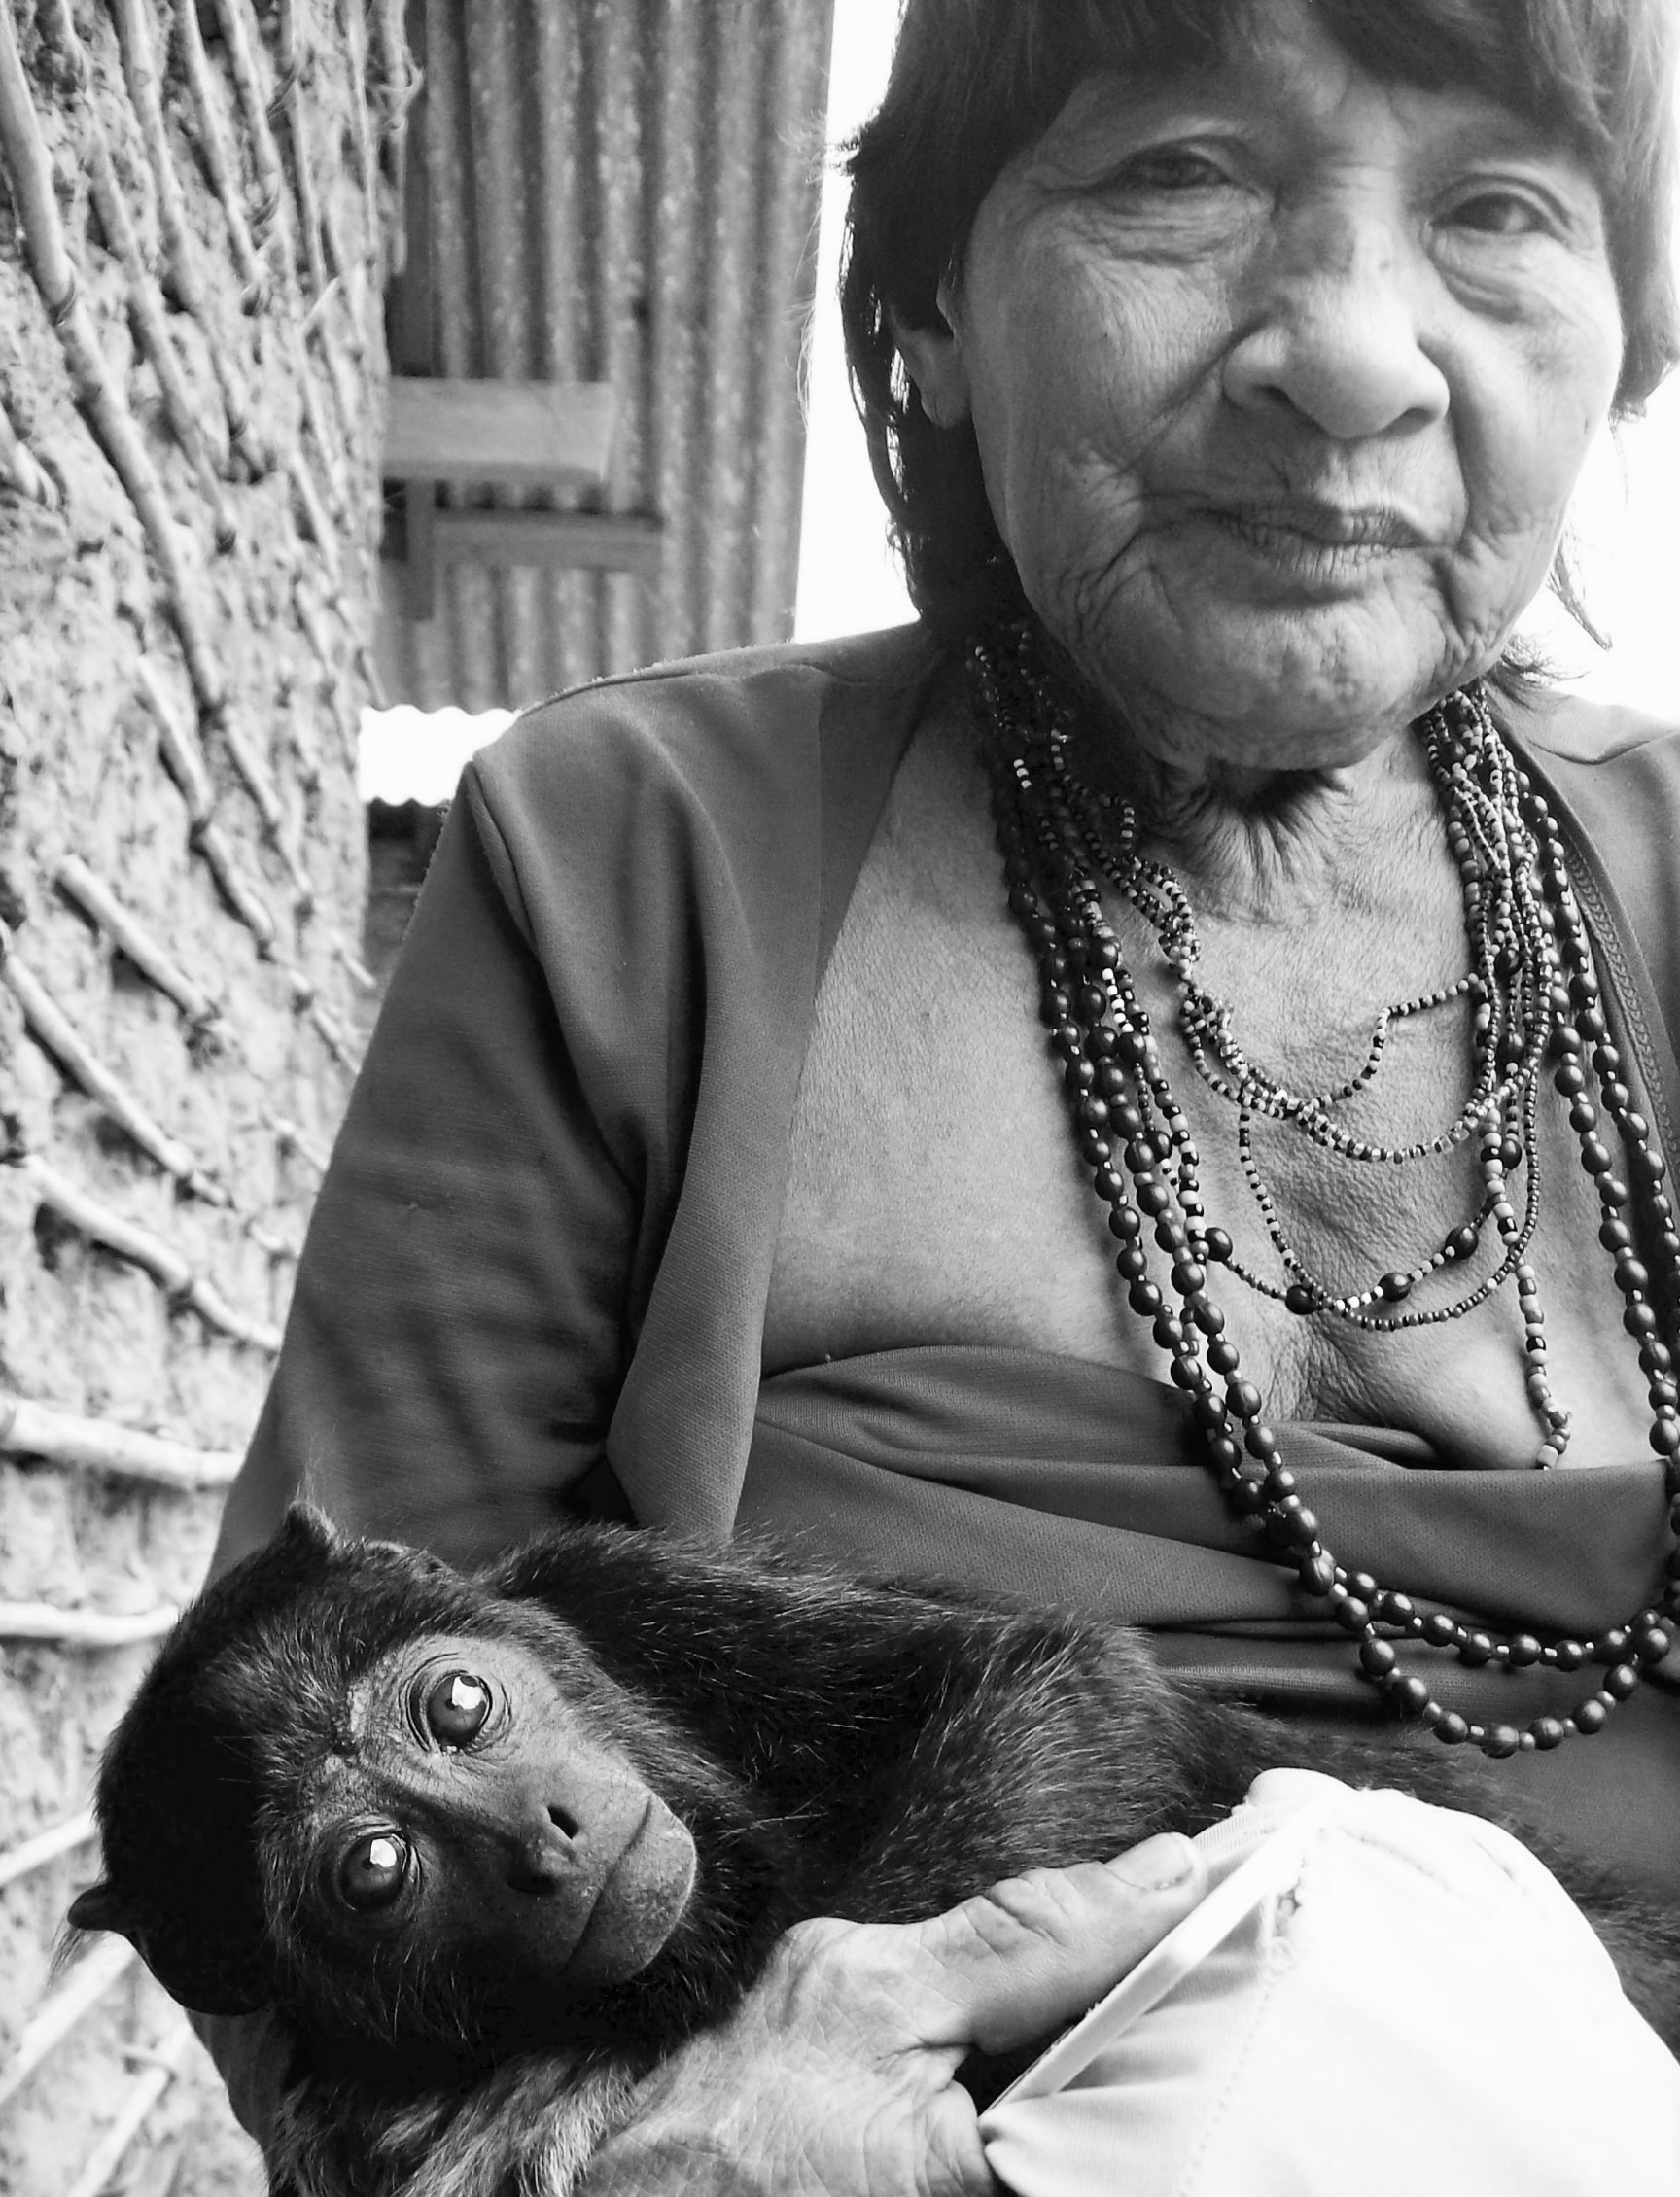
\includegraphics[width=100mm]{./imgs/100_3892}
%\caption{Amy͂ Paranawãja e seu capelão de criação (aldeia Tiracambu, 2008).}
%\end{figure}

O ano era 2007. Em uma manhã úmida de inverno, eu acompanhava a família
de Wirahoa em mais uma caçada. Após sairmos da aldeia, atravessamos uma
roça de mandioca, seguida de uma capoeira velha, \textit{komỹna}, que
separava a floresta --- \textit{haka'a}, ``minha floresta'' --- do espaço da
aldeia --- \textit{haripa}, ``minha casa''. Antes de adentrarmos a floresta,
avistei um grupo de borboletas brancas levantando voo enquanto
passávamos. Devido à beleza da cena, indaguei a meus companheiros: ``como
vocês chamam borboletas como aquelas?''. Wirahoa me respondeu que
tratavam-se de borboletas brancas, \textit{panỹ xũa}, e emendou:
\textit{kamixa panỹ}, ``são as borboletas do jabuti''. Um pouco confuso
perguntei se era o nome da ``espécie'' de borboleta, e ele me disse que
não, que as borboletas eram \textit{kamixa nima}, em uma tradução literal,
``animais de criação dos jabutis''. Foi a primeira vez que mencionaram o
fato de um animal --- por assim dizer --- ter outro como animal de criação.
A partir de então me relataram um processo muito característico da
etologia Guajá, em que animais têm relações do tipo \textit{riku} (de
criação); alguns serão \textit{nima} (crias) ou \textit{jara} (criadores) de
outros, domesticando-se conforme uma \textit{teoria da relacionalidade}
bastante particular.

Desta forma, muitos seres se enxergam como \textit{jara} de outros
\textit{nima}, e como tal são vistos pelas criaturas com que se
relacionam. Formigas tucandeiras são animais de criação de macacos
capelães; os porcos do mato criam algumas espécies de cobra; os poraquês
(peixes elétricos) são donos de diversas espécies de peixes e, por sua
vez, animais de criação para os jacarés --- \textit{jakare} \textit{nima},
``xerimbabo do jacaré''; assim como toda espécie de mel, dentre as
dezenas existentes, pertencerá a algum ser que é seu \textit{jara}. De uma
maneira geral, muitos animais caçados pelos humanos são animais de
criação de outros animais. Em todos esses casos encontramos a mesma
relação, \textit{jara} (criador) → \textit{riku} (a relação) → \textit{nima}
(cria), em que \textit{riku} é o vetor destes polos. A proposta deste
capítulo é apresentar as muitas formas com que a relação \textit{riku}
opera no mundo Guajá. A hipótese aqui defendida é que o parentesco, tal
como discutido no capítulo anterior, é uma das formas em que a relação
\textit{riku} aparece, mas não a única. Veremos aqui como tal relação
atravessa diferentes formas de subjetividade, e dentre elas, como vimos,
está também a conjugalidade. Muito embora os Guajá não mencionem nenhum
verbo para \textit{casar}, em nossas conversas o casamento era explicado
pela ideia de \textit{riku}; a relação entre homens e mulheres que vivem
juntos. Para um \textit{awatea}, homem ou uma mulher, estar ligado a
alguém por ``casamento'' significa estabelecer com seu cônjuge uma relação
do tipo \textit{riku}.

\section{criando seres}

Na língua guajá a raiz do termo para os animais de criação é \textit{ima},
podendo ocorrer associado a um nome, sob a forma \textit{nima} ``animal de
criação de'', como nos exemplos \textit{Pakwa'ĩ nima} --- ``o animal de
criação de Pakwa'ĩa'' ou \textit{Amỹ nima} --- ``o animal de criação de
mamãe''; além de poder ocorrer associado a marcas de pessoa, como no
exemplo \textit{hanima}, ``meu animal de criação''. Em meu texto oscilarei
entre a utilização das formas \textit{nima} e \textit{hanima}. A categoria
complementar a \textit{ima} é \textit{ja}, que aparece na maior parte dos
contextos pronunciada como \textit{jára} ou \textit{jará}, a depender da
variante linguística do falante. \textit{Ja}- é cognato do \textit{jar}
waiãpi apresentado acima, e um conhecido termo tupi-guarani cuja
tradução mais conhecida é ``dono'' ou ``mestre''.

Os animais domésticos, por exemplo, quase sempre capturados na floresta,
são desses seres \textit{nima} de quem os humanos são \textit{jara}, e com
quem estabelecem uma relação do tipo \textit{riku}. O termo \textit{nima}
dificilmente poderá ser compreendido sem lançarmos mão de seu inverso,
ou complemento, que é a ideia de \textit{jara}, e ambos só serão
apreendidos se postos em relação a partir da ideia de \textit{riku}. Para
o caso Guajá, a relação existente entre um \textit{jara} e um \textit{nima}
é do tipo \textit{riku}, isto é, todo \textit{nima} será ``criado'', segundo a
tradução guajá, ou estará associado a um \textit{jara}. Tal relação
figurará em diversos ambientes, como a conjugalidade, caça e cosmologia.

As pessoas da aldeia Juriti não faziam um uso deliberado da ideia de
``dono'' para traduzir \textit{jara}. Ainda assim, penso que se alguma
tradução pudesse ser feita, certamente a ideia de ``dono'', tal como
aparece em outras etnografias, seria um termo aceitável. Por exemplo, em
2008, os funcionários do \textsc{pin} Juriti compraram um jumento --- na verdade,
uma jumenta --- a fim de ajudar os Guajá durante os trabalhos na roça,
principalmente para carregar os pesados fardos de mandioca e arroz.
Embora eventualmente utilizassem a jumenta como um animal de carga, o
uso que os Guajá deram ao animal não correspondia aos anseios dos
servidores do posto. Nos dias de trabalho de roça, enquanto os homens
iam e voltavam da lavoura, muitas vezes atravessando brejos, carregando
pesadas cargas de mandioca e outros cultivares, as crianças passeavam
animadamente pela capoeira com a jumenta, sem que ninguém se importasse
em colocá-la para trabalhar --- com exceção dos funcionários do posto, que
reclamavam bastante e com frequência tentavam intervir nessa dinâmica,
mostrando o que deveria ser feito com o animal. Os Guajá, no entanto,
sempre voltavam a deixá-la como um animal doméstico, cuja principal
função é viver como tal, livre. Entretanto, tal como os cachorros que os
ajudavam na caça por ser um \textit{karai} \textit{nima}, um animal de
criação dos \textit{karaia}, as potencialidades produtivas da jumenta eram
também aproveitadas, mas muito eventualmente. Dentre todas as pessoas, o
pequeno Takwaria, na época com nove anos de idade, era quem melhor
cuidava do animal: dava-lhe comida; encaminhava-o para sua choupana para
que não pegasse chuva e, caso a jumenta sumisse, o menino quase sempre
sabia do seu paradeiro. Como os adultos não dispensaram especial atenção
ao animal para cuidar e alimentá-lo, o menino Takwaria desempenhava
essas tarefas de bom grado, e passava boa parte do tempo colocando
crianças menores no lombo da jumenta para se divertirem, ou mesmo
providenciando a cangalha para o animal carregar fardos para seus pais e
familiares. A respeito do animal, todos diziam ser ``a jumenta de
\textit{Takwaria}'', ou ``\textit{Takwari} \textit{nima}'', ``animal de criação do
Takwaria''. Devido a seu envolvimento com o bicho, o pequeno Takwaria era
tido por todos como \textit{jumenta} \textit{jara}. Nesse caso, \textit{jara}
pode, e deve, ser traduzido literalmente por ``dono''. Dono, não como
alguém que exerce propriedade sobre algo, mas como aquele que alimenta,
cuida e cria um ser como um \textit{nima}, ``o animal de criação dele''.

A ideia de ``domesticação'', que atuaria em diversas esferas, desde os
animais de criação até a relação entre afins em potencial, de uma forma
geral, não representa novidade nas análises de diferentes grupos
amazônicos. No entanto, o que deve ser verificado é se tal ideia poderia
ser concebida conjugada com outras relações que extrapolariam a ideia de
domesticação. Explicando melhor: é possível encontrar na relação de
``domesticação'' de seres --- que percebo ser deveras atuante entre os Guajá
--- elementos que permitam pensar formas mais amplas de socialidade?
Formas que conjuguem as esferas do parentesco e da cosmologia?
Interpretar as relações entre ``senhores'' e ``seres de criação'' e suas
ideias de ``mestre'', ``dono'' e criatura --- presentes em muitos grupos da
região --- é o ponto de partida para minha investigação. No caso Guajá, é
colocado que entre um ``dono'' e uma ``criatura'' foi estabelecida uma
relação, \textit{riku}.

Desta forma, a ideia aqui é também refletir sobre questões relativas à
figura dos donos na Amazônia, propondo, junto com o capítulo anterior,
um diálogo com um dos aspectos menos explorados do tema, que é a relação
deste com a conjugalidade. Alego que, para os Guajá, as relações
recortadas dos universos dos fenômenos tratados como ``familiarização'' e
``maestria'' são não apenas coextensivas ao campo do parentesco, como
também revelam uma concepção muito particular do que seja a relação
conjugal. Apesar de dialogar com a conhecida imagem dos ``donos de roça'',
``donos de animais'', ``das águas'' e outros correspondentes, tomo o
conceito de dono aqui como uma imagem-guia (nos termos de Strathern,
2006, p.\,208) a ser mobilizada em sua definição relacional, pensada tanto
para as relações de familiarização quanto para a conjugalidade. A
continuidade ontológica entre maestria e casamento --- cosmologia e
sociologia --- para os Guajá não remete a uma alegoria simbólica que, por
analogia, se conecta a termos conjugais humanos e não humanos (tal como
um xamã e suas esposas celestes; ou casamentos intraespecíficos
mitológicos). Não se trata de uma conjugalidade cosmológica, mas a
própria relação de casamento é concebida como de ``criação'' e, de muitas
maneiras, homóloga a outras relações no mundo.

\begin{center}\adforn{68}\end{center}

Embora não apresente em seu trabalho referências sobre as ideias de
\textit{riku} ou \textit{jara}, Cormier dedicou sua atenção aos animais
criados nas aldeias e às relações estabelecidas entre eles e os humanos.
Seu trabalho é particularmente interessante por trazer dados de um dos
aspectos sociais mais ricos da vida Guajá, isto é, a forma quase
obsessiva com que transformam filhotes de animais selvagens em animais
de estimação. Em linha gerais, a autora argumenta como o idioma do
parentesco pode informar, em muito, o modo como as pessoas se relacionam
com esses animais, principalmente na relação entre as mulheres e os
macacos-capelães (\textit{Alouatta belzebul}), que detêm um \textit{status}
diferenciado.\footnote{Ver Cormier, 2003, pp.\,111--128.}

Cormier (\textit{op.\,cit.}), ao apresentar a relação que os Guajá estabelecem com
seus animais de criação (\textit{pets}), mantidos na aldeia muitas vezes
em grandes quantidades, observa, inclusive, que eles podem chegar a
ultrapassar o número de seres humanos em uma aldeia. São macacos, jacus,
quatis, jacamins, cotias, pacas, tartarugas, porcos e até filhotes de
jaguar, criados pelas mulheres, crianças e, em alguns casos, pelos
homens. Da captura à soltura dos animais, o livro apresenta bem o
fenômeno. Uma das conclusões a que a autora chega é que os \textit{hanima}
seriam uma categoria intermediária entre os Guajá e os animais e
plantas, seres da floresta. Em sua apresentação, ela afirma que o termo
\textit{hanima} é ``ambíguo'', pois aparece tanto ao se referirem aos
animais criados como, por vezes, para animais caçados (Cormier, 2003, p.
94).

Essa ``ambiguidade'' observada pela autora é, no entanto, resultado do que
considero um deslize em sua análise. O equívoco está em tratar a ideia
de \textit{ima} (\textit{hanima}, como citado pela autora) como uma
categoria em si, fruto de uma mera relação local das mulheres com esses
animais. Mesmo as mulheres que, segundo Cormier, tornam-se ``mães'' desses
seres não são apresentadas, em seu trabalho, por meio do termo que os
próprios Guajá utilizam para se referir às donas de um animal, \textit{jara}. 
A ideia de \textit{nima}, por ser um termo relacional,
contraparte, \textit{jara}, não pode ser entendida sem esse inverso
complementar. Sendo assim, veremos que animais de caça são \textit{nima}
de outros seres, isto é, estão relacionados a outros seres (humanos ou
não humanos) da mesma forma que os animais de criação de uma aldeia
estão relacionados aos Guajá.

Como mencionei anteriormente, vejamos um pequeno inventário de espécies
animais que mantêm entre si relações do tipo \textit{riku}, em que uns são
\textit{jara} e outros, \textit{nima}.

\begin{enumerate}
\item
Tal como um tipo de borboletas brancas, \textit{panỹ xũa}, estão associadas aos jabutis, \textit{kamixa}, um tipo de tucano chamado \textit{kakỹa} é animal de criação, \textit{nima}, para os macacos cuxiú, \textit{kwixua}. Quando cantam, esses tucanos o fazem para chamar seus \textit{jara}, os cuxiú

\item
O veado mateiro, \textit{arapaha}, tem a cotia, \textit{akwixia}, e uma  outra espécie de borboleta, \textit{panã}, como ``animal de criação'', \textit{nima}

\item
A cotia é ``dona'', \textit{jara}, do esquilo quatipuru (ou caxinguelê), chamado \textit{tamakaja}

\item
O macaco capelão, chamado \textit{waria}, é ``dono'' \textit{jara} da formiga tucandeira, \textit{takya}, e do macaco-da-noite, \textit{aparikya}. Segundo os Guajá, a relação entre essas duas espécies se dá, pois tanto o capelão quanto o macaco-da-noite apreciam as áreas das árvores mais protegidas por folhas, mais escuras e seguras, diferentemente de outros macacos, não tão exigentes

\item
Os porcos queixadas, \textit{xahoa}, são ``donos'', \textit{jara}, da cobra surucucu, chamada \textit{arykukua}

\item
Os macacos-prego, \textit{ka'ia}, são ``donos'', \textit{jara}, do sagui \textit{atamaria} (\textit{saguinus} \textit{midas} \textit{niger})

\item
Um formigão chamado \textit{tapiuhua} é dito \textit{tapi'i} \textit{nima}, ``ser de criação da anta''

\item
O pássaro surucuá-de-barriga-vermelha (\textit{Trogon curucui}), chamado \textit{arakua}, é um \textit{tatu} \textit{nima}, isto é, um ``animal de criação dos tatus''

\item
O pássaro chora-chuva-preto (\textit{Monasa} \textit{nigrifons}), chamado \textit{jawanĩa}, é um \textit{wari} \textit{nima}, ``animal de criação'' para um capelão

\item
As cigarras \textit{jakaramuhũa} são interpretadas como \textit{hwa'ĩ nima}, um ``ser de criação'' da palmeira babaçu

\item
As aranhas caranguejeiras, \textit{janũa}, são \textit{ka'i nima,} ``animais de criação'' do macaco prego

\item
Os sabiás são animais de criação, \textit{nima}, das capivaras, chamadas \textit{kapijawara}

\item
As araracangas, \textit{ararakỹa}, são \textit{nima} dos queixadas, \textit{xahoa}

\item
Os esquilos quatipurus (\textit{Sciurus aestuans}), chamados \textit{tamakaja}, são ``animais de criação'', \textit{nima}, dos quatis, \textit{kwaxia}

\item
Um tipo de tatu chamado \textit{tatu} \textit{tapajnia}, por ser grande, é chamado \textit{tapi'i} \textit{nima},
``animal de criação das antas''

\item
O jabuti, \textit{kamixa}, e o jabota, \textit{kamixatua}, são \textit{nima} para as jiboias (\textit{majhua})
\end{enumerate}

Nos rios, '\textit{ya}, peixes e outros seres também mantêm relações
do tipo \textit{riku}:

\begin{enumerate}
  \setcounter{enumi}{16}
\item
A piaba, \textit{hipija}, é também chamada \textit{xaho pira}, ``peixes do queixada'', pois são animais de criação dos queixadas

\item
Uma enguia chamada \textit{mahua} é um \textit{manaky} \textit{nima}, um animal de criação do poraquê

\item
O poraquê, \textit{manakya}, por sua vez, é ``dono'', \textit{jara}, de diversos peixes de um rio

\item
O jacaré, \textit{jakarea}, é \textit{jara} da capininga, \textit{jaxajhua}, poraquê, \textit{manakya}, traíra, \textit{tara'yruhua}, dentre outros peixes
\end{enumerate}
  
Além dessas, uma infinidade de relações semelhantes são traçadas, que
muitas vezes associam seres e elementos --- que para nós são diversos
entre si --- como nos casos abaixo:
    
\begin{enumerate}
  \setcounter{enumi}{20}
\item
Os peixes gurijuba, \textit{hi'ijua}, são \textit{jara} de um pequena cobra chamada \textit{i'ĩ jumaja}

\item
Os peixes traíra, \textit{tara'yruhua}, são \textit{jara} de uma cobra chamada \textit{tara'yruhu maja}
\end{enumerate}

Em todas essas situações encontramos a mesma relação \textit{jara} →
\textit{riku} → \textit{nima}, em que \textit{riku} é o vetor desses polos.
Tal forma de relação se mostra bastante normativa, ao mesmo tempo que
aberta --- parafraseando Descola (2006, p.\,138) ---, e por isso não devemos
pensar que os Guajá mantêm um inventário de todas as relações possíveis,
entre todos os seres que vivem em seu mundo; não faz sentido montarmos
um vasto quadro, com inúmeras dessas relações e possibilidades para uma
coerência total do universo. O que é colocado, muito mais do que quem é
\textit{jara} ou \textit{nima} de quem, é o fato de muitos seres só existirem
na medida em que estejam estabelecidas relações como esta, isto é,
alguns seres serão ``criados'' por outros ou ao menos, e para me basear
fielmente na tradução linguística, ``estarão com'' outros.

Nos chuvosos meses de janeiro a março, os mosquitos pium, \textit{pi'ũa},
atacam com intensidade algumas aldeias, quando formam verdadeiras
nuvens. A concomitância do aparecimento dos piuns com a época do pequi,
\textit{myky'á}, é ilustrada por uma relação de continuidade
sociocosmológica entre insetos e frutos. Ambos aparecem na mesma época,
e o pequi é pensado como \textit{pi'ũ nima}, ``seres de criação dos piuns'',
e os piuns, por sua vez, seriam \textit{myky'a jara}, os ``donos do pequi''.
O agradável sabor do pequi sempre será desfrutado ao lado das
inconvenientes picadas dos piuns; foram ``misturados'', \textit{mijamema}, e
sempre aparecerão ``juntos'', \textit{pyry}. O maior empecilho para que tal
relação continue em curso é o desmatamento que hoje assola o oeste
maranhense. Os Guajá lembram que as chuvas são enviadas por um grupo de
\textit{karawara}, ``humanos celestes'', que controla as águas e as manda
periodicamente para a floresta, pois, embora vivam historicamente de
caça e coleta, a floresta é como um lugar cultivado (como sabemos que
ocorre em outras cosmologias amazônicas, como nos Achuar e os Waiãpi).
Os \textit{karawara} não enviam chuva para as áreas desmatadas, porque
onde não existem árvores não existem frutas e não haverá animais para
delas se alimentar. Por serem também caçadores, \textit{watama'a}, estes
seres cultivam as florestas para que os animais existam e eles mesmos
possam caçá-los na Terra. O desmatamento --- que, como sempre, traz
consequências cosmológicas gravíssimas, cataclísmicas, para os povos
ameríndios --- pode estraçalhar relações como esta, uma vez que existirá
um mundo com piuns e sem pequizeiros; com criadores, ou donos, e sem
criaturas.

Por vezes, \textit{jara} serão os animais que consomem com mais
intensidade determinados frutos. Por isso as pacas são \textit{jara} do
frutinho da árvore maria-preta chamados \textit{wawa'ã}. Não que animais
como cotias, veados, antas, porcos, dentre outros, não se alimentem
desses frutos, mas são as pacas as que os consomem com mais intensidade.
Eles são a ``comida da paca'', \textit{kararuhu nimi'ũa}, ou simplesmente
``estão junto'' às pacas, \textit{kararuhu pyry}, por isso as pacas são
\textit{jara}, ``criadoras''. O mesmo acontece com várias outras espécies
vegetais, e algumas recebem na classificação o nome do animal dono, como
``mandioca de cotias'', \textit{akwixi tyrymỹa}, ``pequis de tucanos'' e
``comida de capelão'', \textit{wariwa}, dentre tantas outras. Da mesma
forma, os cipós, \textit{ipoja'a}, em geral são tidos como ``criados'' pelos
macacos capelães e chamados de \textit{wari nima}, ``seres de criação dos
capelães'', justamente pelo uso frequente que esses primatas fazem deles
para se locomover.

Em certa ocasião, conversando com Pira'ima'ã, ele me informou que o
\textit{jara} da árvore angelim, \textit{jari'ia}, era um corujão branco
chamado \textit{puhupuhua.} Quando perguntei em seguida se havia
\textit{jara} para a maçaranduba, \textit{mixiranyka}, ele respondeu serem
\textit{Mai nima}, uma espécie de ``resposta padrão'', dada quando não se
``sabe'' sobre o \textit{jara} de determinado ser, uma vez que muitos
seres, direta ou indiretamente, são pensados como \textit{Ma'i
rimijapokera}, ``criaturas de \textit{Maíra}'', em uma tradução literal
``objeto da criação de \textit{Maíra}'' (Magalhães, 2010, p.\,211). Só então
percebi que as questões que eu colocava soavam um tanto desconexas, pois
a pergunta que a mim, etnógrafo, passaria a fazer sentido não seria
``este ser (animal, vegetal) tem dono?'', como inicialmente eu
improvisava, fazendo uso da estrutura da língua portuguesa, porém
mesclada a palavras do léxico guajá. Minhas questões eram entendidas de
outra forma, uma vez que a língua guajá não adota nenhuma partícula
interrogativa que exprima a ideia de uma existência abstrata (ou
absoluta), algo como o verbo ``haver'' e ``existir'', como aparecem nas
formas interrogativas do Português, em uma pergunta do tipo ``Existem
luas em Marte?'' ou qualquer outra questão que prescreva uma existência
absoluta de algo. A partícula interrogativa \textit{mõ}, na língua guajá ---
cuja função é introduzir perguntas de informação --- sempre aparece
seguida de sufixos marcadores de tempo, espaço e posição, cujas ideias
podem ser traduzidas --- segundo Magalhães (\textit{op.\,cit.}, p.\,78) --- como ``para
onde'', ``de onde'', ``com que'', ``quantos'', ``quando'', ``qual dos/\,das'', ``qual'', e
``cadê'', ``onde''. No exemplo: \textit{mõ poho ta mĩpe}, ``Para onde vocês vão?'',
temos \textit{mõ} como partícula interrogativa (de informação) e
\textit{mĩpe} como partícula que exprime o sentido da pergunta.\footnote{Além
  de \textit{mĩ-pe} no final da frase, como no exemplo acima, a partícula
  \textit{mõ} ainda pode aparecer combinada com as partículas: \textit{mijỹ}
  -- ``de onde?''; \textit{mimehẽ} -- ``quando?''; \textit{mijẽ} -- ``com que'',
  ``quantos?''; \textit{minawỹ} -- ``qual dos/\,das''; \textit{mõa} -- ``qual'';
  \textit{mõ} -- ``cadê'', ``onde''.}

Embora o termo \textit{ikwẽe} possa ser traduzido por ``permanecer'',
``existir'', ``viver'', não faziam sentido minhas perguntas a respeito das
relações do tipo \textit{jara} e \textit{nima} a partir de ideias do tipo ``há''
ou ``não há'' criadores e criaturas nas diversas situações. As questões
seriam melhor compreendidas em formas como ``\textit{Mõ myky'a jara mõa}?'',
isto é, ``Qual o \textit{jara} da árvore de pequi?'' Os Guajá me ensinaram
que a pergunta certa a fazer é \textit{ma'awa jara?}, em outras palavras,
``que gente é \textit{jara}?'' (ou ``quem é o \textit{jara} {[}deste ser{]}?''),
de maneira que não há significação em perguntar se tal ser ``tem'' um
dono, pois em tese todos --- ou quase todos --- o terão. Isto posto, o
repertório de combinações é bem amplo, tanto que em diversas situações
não conseguiam saber qual era o \textit{jara} de determinado ser, embora
soubessem que um ser seria possuído.

Da mesma forma, as respostas nunca eram taxativas e, quando feitas em
português, eram sempre respondidas com um ``\textit{parece que é}''. Meus
amigos raramente respondiam a uma pergunta com ``sim'' ou ``não'', mas com
``parece ser''. Na língua guajá a partícula epistêmica similativa
\textit{rawỹ}\,\textit{nawỹ}\,\textit{nawyn} indica algo que se supõe verossímil, e
essas formas podem ser traduzidas como ``aparentemente'',\footnote{Para o ver o
funcionamento desta partícula na língua guajá, ver Magalhães, \textit{op.\,cit.},
p.\,116.} O melhor exemplo está na pergunta ``o que é?'', que na língua
guajá aparece como \textit{ma'a nawỹ} e deve ser traduzida como ``o que
parece ser?'' Quando eu lhes bombardeava com perguntas, ainda que em
português, quase sempre as respostas iniciavam com um ``parece que\ldots{}''
ou, ``para mim é\ldots{}'', na forma \textit{a'e apo}, ``deve ser'', ``parece'', com
outra partícula epistêmica que indica possibilidade (ou não certeza).
Podemos pensar também aqui que tal recurso linguístico se relaciona,
segundo Lima (1996), a certa ``noção de ponto de vista'', tal como
observado pela autora ao encontrar um recurso linguístico muito
semelhante entre os Yudjá. Segundo a autora:

\begin{quote}
Em meu trabalho de campo, uma das primeiras coisas a chamar-me a atenção
foi a marca indelével, mas muito misteriosa, da noção de ponto de vista.
Certas frases, ditas para mim em português, como ``isso é bonito para
mim'', ``bicho virou onça para ele'', ``apareceu caça para nós quando
estávamos fazendo a canoa'', pareciam remeter exclusivamente à estrutura
gramatical de uma língua que eu não dominava, mas que transparecia no
português dos Juruna. Depois que comecei a arranhar algumas frases, as
construções que ensejavam tais traduções nunca deixaram de soar
estranhas; dentre as práticas juruna mais difíceis de assimilar eu as
destacaria, em primeiro lugar e sem hesitação. \textit{Amãna ube wï} ---
não é fácil dizer isso sem se desconcertar, desagradavelmente ou não.
Sentia-me dizendo ``choveu para mim'', e não ``choveu onde eu estava''.
Essa maneira de relacionar à pessoa até mesmo os acontecimentos mais
independentes e alheios à nossa presença deixa sua marca na cosmologia
juruna, mas nem presumo que todas as categorias gramaticais tenham o
mesmo papel em uma cultura, nem acredito que exista a mais remota
possibilidade de algum de nós se colocar na pele de um Juruna para
captar o sentido que assumiria a vida humana em uma situação em que,
para nós, de repente, se tornaria aceitável, ou mesmo perfeitamente
justo, dizer: chove para mim. Esse sentido diria respeito no máximo a
uma virtualidade que está em nós, virando-nos pelo avesso.\footnote{Lima, 1996,
p.\,30.}
\end{quote}

As formas Guajá, semelhantemente ao que a autora argumenta para os
``Juruna'', se apoiavam em dativos e locativos a ponto de descrições
cotidianas serem sempre acompanhadas também de um ``para ele'', que na
língua guajá aparece sob as formas ``\textit{ipe}'', literalmente ``para
ele'', ou \textit{ihape}, ``para mim''. Em certa ocasião um homem
contava que sua canoa havia virado. Quando me relataram a conversa
disseram \textit{Kanũa jare ipe}, literalmente, ``a canoa virou para
ele''. Ou mesmo quando repetiam a fala de alguém, ela sempre era
acompanhada desse ``para ele'', como certa vez eu mencionei que a
pequena Aparana'ia já estava crescida e, ela, sem entender o meu
português, questionou sua mãe por meio de uma interessante formulação
que é muito usada: \textit{ma'a i'ĩ nipe}?, isto é, ``o que ele disse a
você?'', e a mãe respondeu: ``Ele disse que você está crescida, para
ele!''. No caso da relação \textit{riku}, estabelecida entre um
\textit{jara} e seu \textit{nima}, de maneira perspectivista ela nunca será
absoluta. Como veremos agora, um ser só estará associado, \textit{riku}, a
outro parcialmente.

Esta relação estaria no nível --- digamos --- da \textit{espécie}. São tipos
de animais que se conectam a outros dessa forma. Outros povos também
produzem categorizações entre os animais nesta chave de seres que são
``donos'' de outros. É o caso dos Karitiana, para quem os gaviões-reais
aparecem como ``donos'' dos macacos, da maioria das espécies arborícolas
e de algumas aves, as ``caças do alto''; ao passo que a onça seria a
dona das ``caças de baixo'', como porcos do mato, veados e tamanduás
(Vander Velden, 2012, pp.\,247--257). Tais ideias fazem referência aos
animais como --- digamos --- \textit{espécie}, sto é, tais espécies animais
são donas de tais espécies animais, se atualizando em relações
particulares. Por exemplo, certa vez, enquanto seguíamos os vestígios de
um bando de capelães, encontramos muito próximo ao local a que chegamos
um bando de ouriços-cacheiros, \textit{kwanũa},\footnote{Uma espécie de
  porco-espinho, também conhecida como ``quandú'' (\textit{Coendou
  prehensilis}).} determinados como \textit{wari} \textit{nima}, ``animais de
criação dos capelães. Conseguimos abater um ou dois enquanto
lamentávamos não nos termos encontrado com os capelães. Quando indaguei
a um companheiro de caça se não estávamos, desde o início, no encalço
desses estranhos animais (os ouriços-cacheiros), ele me explicou que as
fezes que encontramos (e seguimos) eram realmente de capelães, porém,
pelo fato de os capelães serem \textit{kwanũ} \textit{jara}, ``donos dos
ouriços-cacheiros, não o admirava termos encontrado os ``xerimbabos'' no
lugar dos ``donos'', que haviam fugido. Assim, para aquele grupo
específico de ouriços, aqueles capelães específicos que perseguíamos
eram seus donos. Da mesma forma que, em outra ocasião, quando andávamos
na floresta seguindo alguns macacos cuxiú, \textit{kwixua}, percebemos
estar perto do bando ao ouvirmos o tucano \textit{kakỹa}, também chamados
\textit{kwixu} \textit{nima}, ``animais de criação dos cuxiús'', voando de uma
copa de árvore à de outra. Desta forma, aqueles tucanos eram seres de
criação, \textit{nima}, do grupo de cuxiús que nós procurávamos, e não de
todos os cuxiús existentes, pois que a relação entre essa espécie de
tucano e esse tipo de primata sempre irá ocorrer.

Um animal sempre será referido pelo nome de seu \textit{jara}, ``seu dono'',
junto com o termo \textit{nima}. Assim, como vimos, o jumento da aldeia
Juriti era chamado \textit{Takwari} \textit{nima}, ``animal de criação de
Takwaria''; ou os macacos da mulher Panapinuhũa são chamados
\textit{Panapinuhũ} \textit{nima}, ``animais de criação de Panapinuhũa''; e
assim por diante. Todas essas pessoas são ditas \textit{jara} de seus
animais criados, da mesma maneira que para um pai ou uma mãe pode-se
dizer \textit{jara} de seus filhos, e animais podem ser de outros, como
acabamos de ver. Se a relação entre os animais de criação e seus donos
aparece como perfilhação, como diversos autores discutem,\footnote{Ver Cormier,
2003 para o caso Guajá; Erikson, 1897, 2012; Fausto, 2008.} ocorre de esta
posição \textit{jara} ser concebida como própria da mãe (e por vezes do
pai) de crianças. Então, como em um ciclo infindável, se uma mulher sabe
ser dona de um xerimbabo ela o é, antes, por saber ser dona de seus
filhos, e antes disso, porque antes de filhos criou mais xerimbabos,
pois as meninas fazem isso desde crianças. Pude ver certa vez o velho
Pirama'ã pegando seu filho ainda bebê, que chorava muito, enquanto
encaminhava a criança a seu filho mais velho, dizendo: \textit{araho ja
pe}!, ``leve-o para a dona dele'', forma sinônima de ``leve-o para a mãe
dele''. \textit{Jara} aqui estaria muito mais próximo do \textit{iwa} Yudjá,
como \textit{aquele que possibilita a vida} de determinados seres (filhos
ou xerimbabos), do que de um ``proprietário'', já que uma das principais
tarefas de qualquer \textit{jara} é garantir o crescimento de alguém
--- \textit{mixa'a}, ``crescimento dele''.\footnote{Este tema tem mobilizado
  diversos debates na antropologia do parentesco contemporânea
  encarnados na discussão em torno da ideia de \textit{nurture}, passando
  ``por análises que, incorporando fenômenos da ordem da troca e partilha
      de alimentos, de suas ressonâncias e efeitos sobre afetos e
      disposições, promovem um questionamento da barreira entre nature e
      nurture que subjaz às concepções modernas do parentesco, assim como,
      inevitavelmente, à grande parte da reflexão antropológica sobre o
      tema'' (Coelho de Souza, 2004, p.\,28; ver também Battaglia, 1985; Strathern,
  1999; Carsten {[}org.{]}, 2004; para a Amazônia, ver Gow, 1997; Overing, 1999; Rival, 1998).} A forma \textit{riku} ocorrerá entre parentes
próximos como uma maneira de produzir consubstanciação conjugal e
proximidade genealógica (Viveiros de Castro, 2002a, p.\,157), bem como
também expressará formas de adoção (Fausto, 2001, pp.\,413--418; Maizza, 2014,
p.\,500).

Trata-se de uma relação assimétrica, orientada, donde um \textit{nima}
sempre ``estará associado'', \textit{riku}, ou ``será criado'',
\textit{riku}, por um \textit{jara}.

% Vejamos o esquema adiante.

% \begin{figure}[H]
% \centering
%   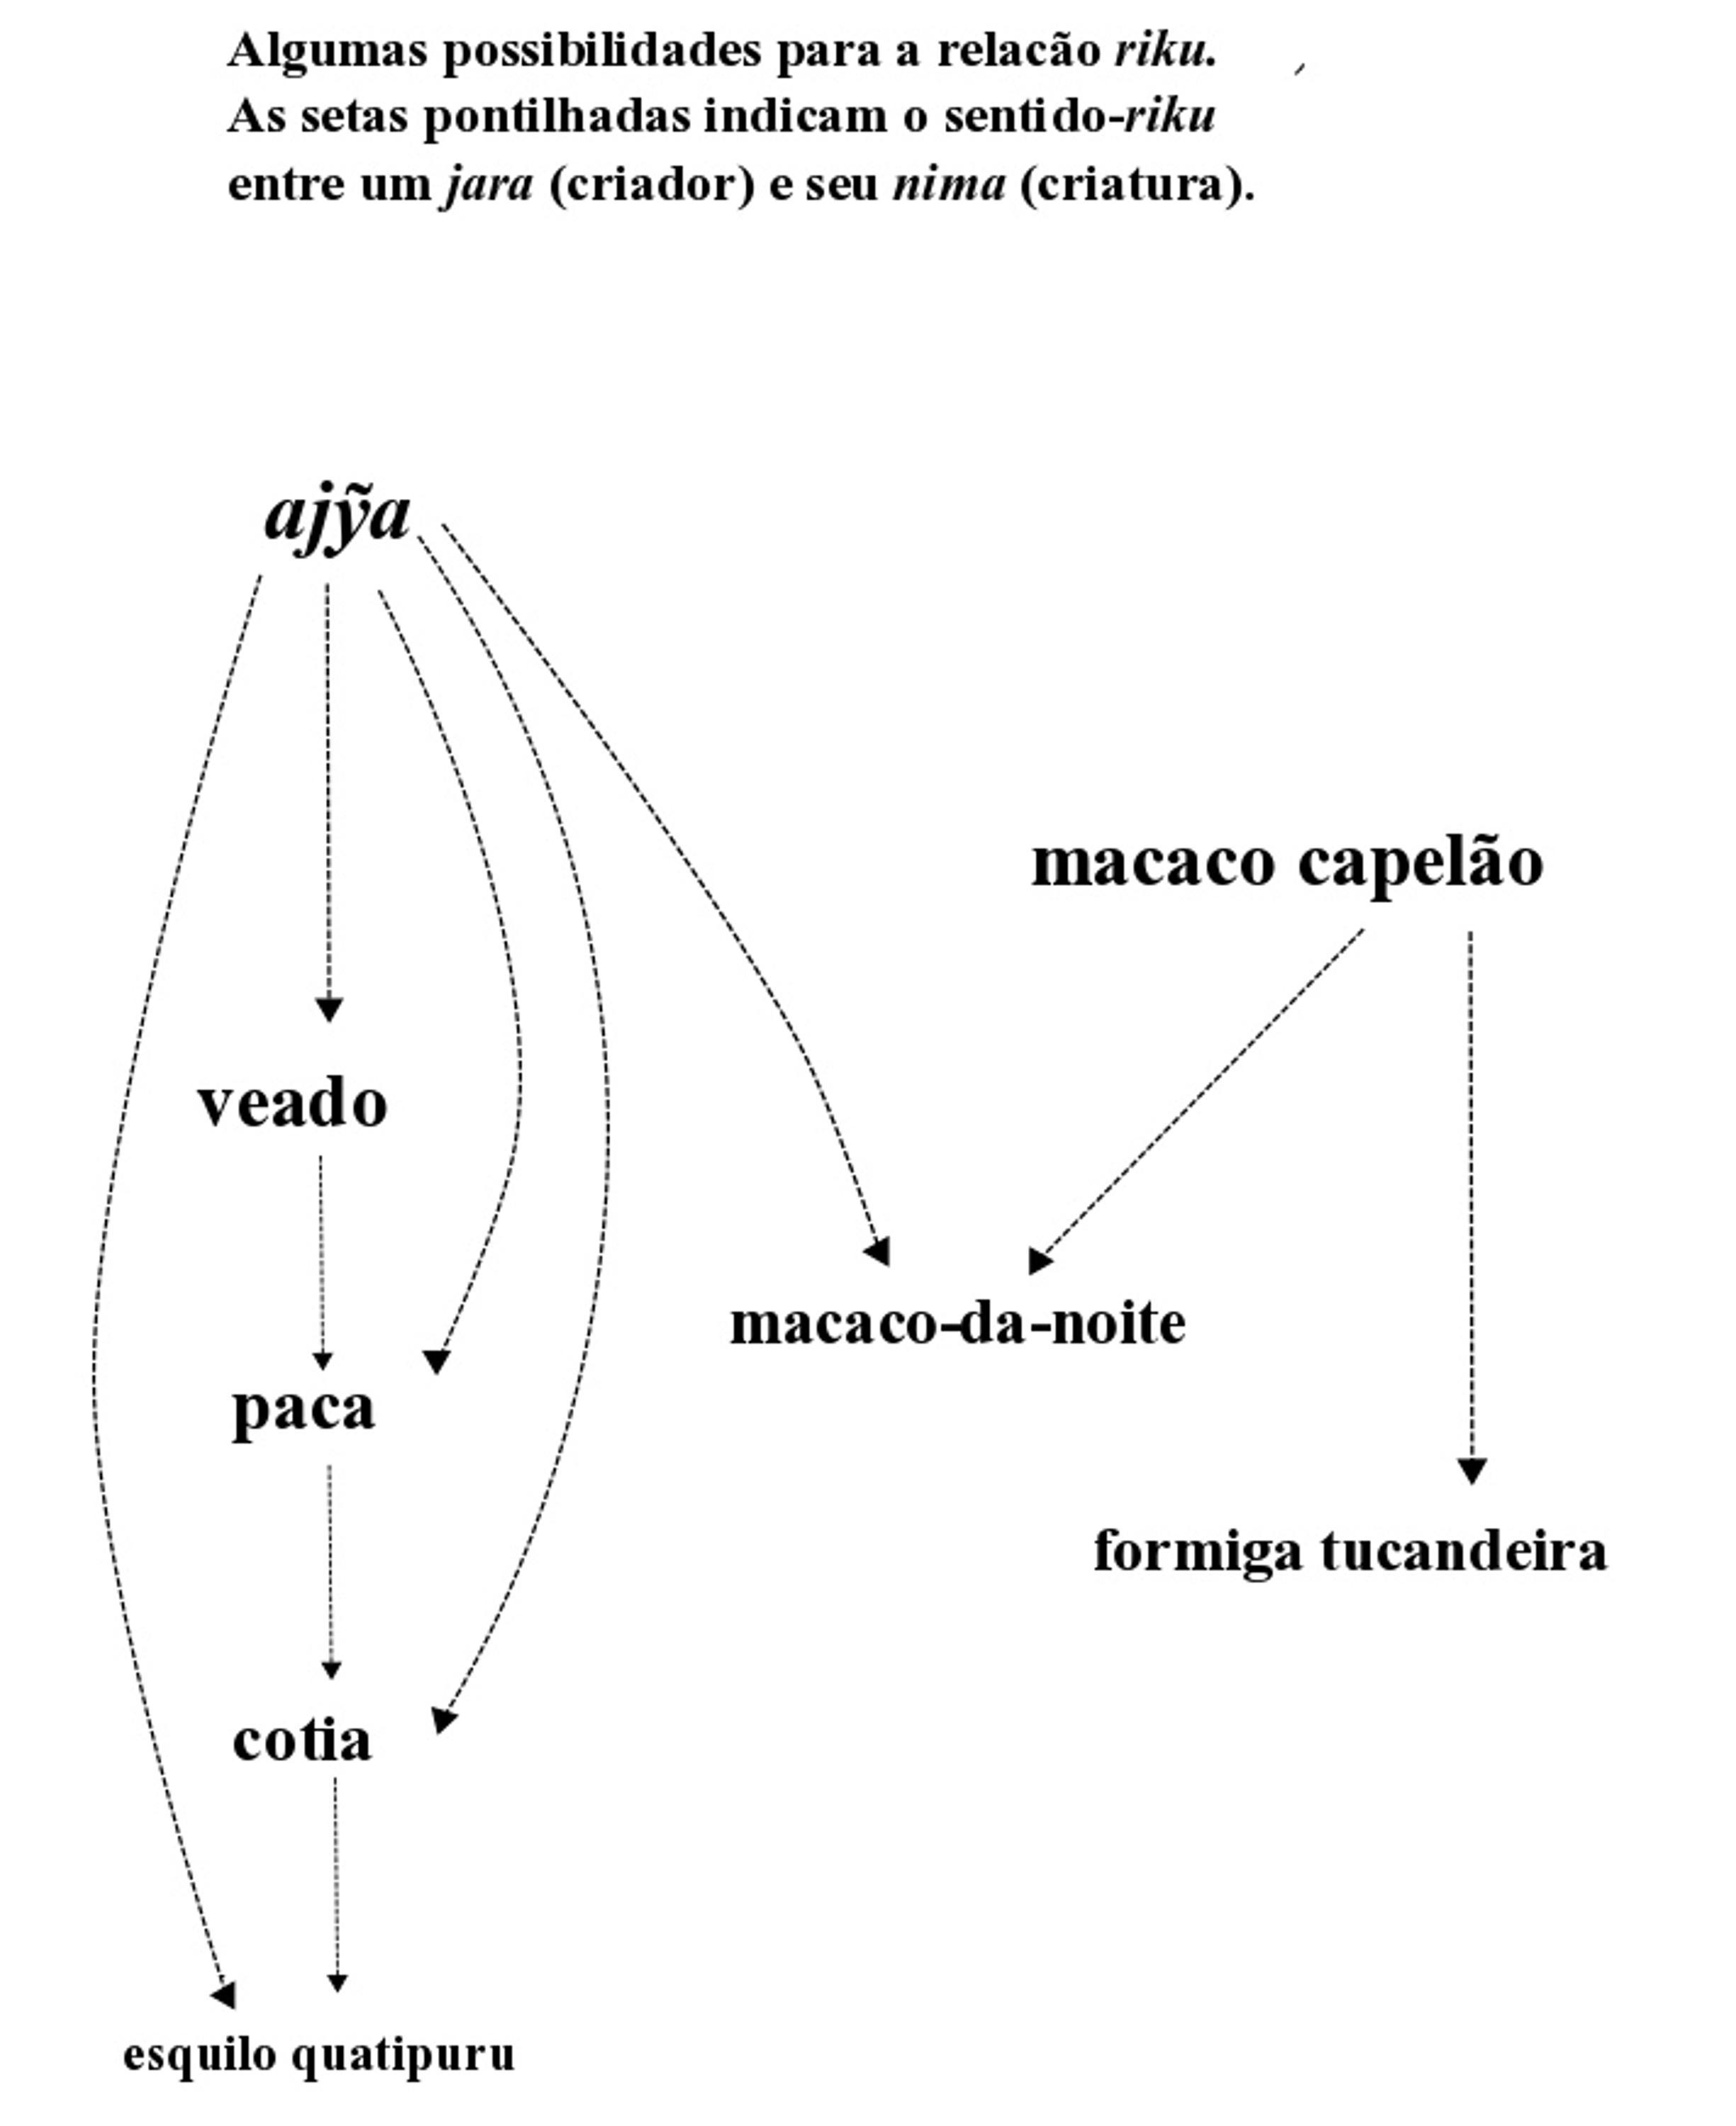
\includegraphics[width=75mm]{./imgs/Figura_11_crop}
% %\caption{}
% \end{figure}

%Figura 11 (10 nos originais)

%A partir do quadro acima, 
No plano cosmológico os \textit{ajỹa} não detêm
qualquer relação de controle sobre os macacos-capelão, \textit{waria},
ambos pertencem, nesse caso, a universos culturais distintos. Enquanto
os animais controlados pelos \textit{ajỹa} estão, de alguma maneira,
associados aos espectros dos mortos e à ``feitiçaria'', \textit{ma'akwa},
propiciada pelo controle dos \textit{ajỹa} sobre seus \textit{nima}
(mucuras, quatis, veados, pacas, cotias, macacos-da-noite), os capelães,
apesar de também deter capacidades agentivas, sobretudo na forma da
vingança pós-caça (como veremos no capítulo 8), fazem parte de um grupo
de animais desejáveis ao consumo em qualquer época e situação.\footnote{Mesmo
  na couvade pós-parto ou reclusão por homicídio que um homem venha a
  experimentar, a carne de capelão --- junto com a farinha de mandioca e
  alguns peixes pequenos --- é a primeira a entrar na dieta tão logo o
  processo se inicie.} Entrementes, como observamos na figura anterior,
os Guajá afirmam que tanto os \textit{ajỹa} quanto os capelães enxergam os
macacos-da-noite como animais de criação, da mesma forma que duas
mulheres diferentes podem manter cotias diferentes como animais de
criação. Parece não se tratar, portanto, de relações do tipo \textit{donos
da espécie} como se os \textit{ajỹa} ou capelães fossem ``os donos'' dos
macacos-da-noite --- um ou mais seres controlando um conjunto homogêneo de
outros seres --- embora, como veremos, também exista tal relação, ainda
que de uma forma menos intensa. Porém, no âmbito geral, a relação
\textit{riku} sugere a ideia de dono \textit{de um} espécime, e não dono
\textit{da} espécie. Um ser sempre será \textit{jara} para si e para um
outro, ou alguns outros. E a relação existente entre um \textit{jara} e
seu \textit{nima} não é incondicional, pois um \textit{jara}, para alguém,
pode ser um \textit{nima} em outra perspectiva; e isso parece estar
acordado entre os diversos seres no mundo: todos parecem saber que
alguém só será um dono \textit{a} \textit{posteriori}, isto é, uma vez
estabelecida uma relação. Se para muitos povos amazônicos a humanidade é
uma qualidade que só pode ser descrita a partir de um ponto de vista\footnote{Lima (1996) relata sobre 
os pontos de vista do corpo ou da aldeia para os Yudjá.} para os \textit{awatea}, a relação \textit{riku} 
--- uma das melhores possibilidades de realização de uma relação humana --- também só poderá se
desenrolar sob um ponto de vista particular.

Os macacos-da-noite podem ser \textit{nima} tanto dos \textit{ajỹa} quanto
dos capelães. Essas são possibilidades balizadas por relações reais que
os Guajá dizem haver entre diferentes seres; e, portanto (ainda segundo
o quadro acima), a formiga tucandeira, \textit{tahya}, é apenas um
\textit{wari} \textit{nima}, ``um \textit{nima} para um capelão''; ao passo que
veado, paca e cotia --- cada um deles --- são \textit{ajỹa} \textit{nima},
``animais de criação para os \textit{ajỹa}''. No entanto, se os
\textit{ajỹa} ``criam'' esses animais, algumas espécies também são dotadas
de um \textit{ponto de vista} que os habilita serem \textit{jara} de outros
seres. Se tomarmos como exemplos a paca, \textit{kararuhua}, o veado, 
\textit{arapaha}, a cotia, \textit{akwixia}, e o quatipuru, \textit{tamakaja}, 
--- animais que estabelecem uma relação do tipo
\textit{riku} entre si ---, podemos ver algo assim:

\begin{enumerate}
\item Os \textit{ajỹa} têm como animais de criação pacas, veados, cotias e
quatipurus
\item  Para os veados, as pacas são os animais de criação
\item Para as pacas, os veados são os donos, \textit{jara}, e as cotias,
animais de criação
\item Para as cotias, as pacas são donas, \textit{jara}, e os quatipurus,
animais de criação
\item Os quatipurus são somente \textit{akuxi} \textit{nima}, ``animais de
criação das cotias'', não ``criam'' algum outro ser
\end{enumerate}

% Verificar tabela
% \begin{figure}[H]
% \centering
%   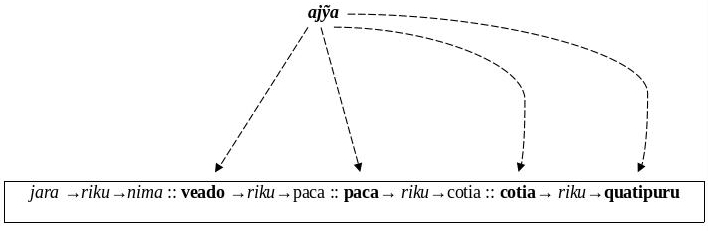
\includegraphics[width=\textwidth]{./imgs/Figura_13}
% %\caption{}
% \end{figure}

%Figura 11

Em paralelo, veados, pacas e cotias, mesmo sendo animais de criação dos
\textit{ajỹa,} mantêm entre si relações de consubstancialidade do tipo
\textit{hapihiara}, ``parentes próximos''. A partir do esquema acima, tendo
como exemplo o veado, este ser é \textit{jara} para uma paca, ao mesmo
tempo que um \textit{ajỹa} será seu \textit{jara}, mantendo relações do tipo
\textit{riku}: uma paca é, para ela mesma, dona, \textit{jara}, de uma
cotia, e animal de criação, \textit{nima}, para um veado. Apesar de
estarem, por assim dizer, na ``área de influência'' dos espectros canibais
\textit{ajỹa}, esses animais são concebidos a partir de uma linha de
continuidade que coloca uns como criadores de outros. Isto não é
meramente um discurso abstrato sobre o mundo, mas implica diretamente a
vida das pessoas, sobretudo no que concerne à caça. O \textit{riku} opera
como um \textit{princípio sociológico} que mobiliza relações entre esses
seres sem necessariamente passar pela perspectiva humana. Os Guajá
apenas \textit{concebem} \textit{como os animais concebem} tais relações. Se
determinadas borboletas são seres de criação dos jabutis, ou se os
cuxiús-pretos o são de macacos-prego, é algo atuante entre tais seres e
escapa ao controle humano. Também não se trata de relações dentro de
relações, mas sim de uma multiplicidade delas, formando-se muito mais
uma pluralidade de \textit{conexões parciais} do que um ``todo'', em que,
supostamente, se encapsulam partes que contenham o todo: trata-se de
\textit{the view from a body rather than the view from above} (Strathern,
2004, p.\,32).

Uma possibilidade para interpretar o problema, tal como os Guajá o
formulam --- como podemos ver no exemplo acima ---, é dada por Lima em um
exercício dialógico com um homem Yudjá (Lima, 2005, p.\,338). Em seu pequeno
diálogo, a autora chega a uma interessante conclusão acerca da relação
entre os humanos e os \textit{'ï'anay}, os espíritos dos mortos. Assim,
há seres que se veem como sujeitos e enxergam outros seres como ``outros''
(mortos, xerimbabos, deuses), sempre do ponto de vista desse sujeito:

\begin{quote}
são três as tomadas em jogo: sua irrealidade para outrem; sua
indubitável existência para si; por fim, a realidade acima de qualquer
suspeita daquele que fala. Se as duas primeiras revelam-se simétricas, a
terceira contém ambas: é ela a assimetria perspectiva, e ela é humana.\footnote{\textit{Idem}.}
\end{quote}

Em seguida a autora reforça que a tal ``assimetria perspectiva'' pode ser
revertida também em benefício dos \textit{'ï'anay}. A partir disso, se
tomarmos o esquema acima dos \textit{ajỹa} e seus \textit{nima}, em que
esses seres criam, \textit{riku}, um conjunto de animais que mantêm também
relações particulares entre si, podemos pensar que ali atua uma
perspectiva do tipo assimétrica para os \textit{ajỹa}, o que habilitaria
tais seres a serem \textit{jara} de um conjunto de outros seres cuja
realidade da relação \textit{riku} só existiria para si mesmos. Nesse
sentido penso que os \textit{ajỹa} sejam \textit{jara} diferentes do que uma
paca é para uma cotia, simplesmente por se colocarem em relação a um
conjunto maior de seres, tal como os humanos, \textit{awatea}, ou
\textit{Maíra,} conseguem fazer.

Trata-se menos de pensar um todo dividido entre, de um lado, donos e, de
outro, seres criados por estes, do que pensar o sistema como uma
multiplicidade de \textit{jara} e \textit{nima}, variando de acordo com as
relações estabelecidas entre os seres --- uma linguagem que concebe
múltiplos pontos de vista, com ênfase no aspecto relacional que aqui
aparece intensamente. A existência dos seres enquanto sujeitos --- a sua
consciência mesma enquanto ser vivente em oposição a outras formas de
vida --- de muitas maneiras está relacionada à possibilidade do
estabelecimento de uma relação do tipo \textit{riku}. É um problema de
posição, do tipo ``isto é dono para mim, enquanto aquilo é xerimbabo
para mim (ou para ele)''. A não totalização dessas relações em
formas-donos do tipo ``donos da caça'', ``donos das águas'', ``donos das
roças'' --- dentre outros que aparecem à exaustão nas etnografias (para um
balanço, ver Fausto, 2008) --- é a marca de como os Guajá pensam tal
relação \textit{riku}, que nesse caso está mais próxima de uma
antimaestria (ao invés de maestria, como propõe Fausto {[}2008{]} para
ideias análogas), uma vez que mestres de criaturas, tal como outras
ontologias prescrevem (algo como propiciadores absolutos), aparecem de
maneira muito fraca aqui. Parafraseando Viveiros de Castro, não estou
com isso advogando que fujamos da noção de dono, ``como se fosse uma
categoria visceralmente antiamazônica'', mas apenas cuidando para não
confundir totalmente o que os Guajá defendem, com o que já foi defendido
para outros povos amazônicos até agora. A relação \textit{riku}
estabelecida entre um \textit{jara} e um \textit{nima}, embora proponha uma
assimetria relacional, não deve ser reduzida à ideia de ``controle'', como
continuaremos vendo.

\begin{center}\adforn{68}\end{center}

Kelly, ao pôr em relação alguns regimes de socialidade amazônicos,
lembra que nas ontologias perspectivistas ``pessoas são esses seres duais
sujeito/\,objeto a que se creditam perspectiva e agência (participam da
cultura e têm uma alma imortal), mas que ao mesmo tempo são objeto de
outra subjetividade (parte da natureza de alguém)''. As posições eu e outro
de coletivos como esses --- seja em relação aos humanos, animais ou
espíritos --- vão variar de acordo com o ponto de vista de quem quer que
esteja se relacionando:

\begin{quote}
Pessoas, portanto, não são nem objeto nem sujeito, mas ambos: o ponto
 de encontro de um Eu reflexivo e da perspectiva do Outro. O contexto
 determinará quanto a qualidade-de-sujeito (\textit{subjectness}) ou a
 qualidade-de-objeto (\textit{objectness}) será prevalecente em uma
 relação. {[}\ldots{}{]} A consciência de uma pessoa de sua
dualidade sujeito-Eu/\,objeto-Outro expressa-se, principalmente, no seu
reconhecimento da possibilidade de se tornar presa de alguém.\footnote{Kelly, 2001, p.\,100.}
\end{quote}

No caso Guajá (e parafraseando Kelly), a consciência de uma pessoa sobre
sua dualidade eu e outro expressa-se, principalmente, no reconhecimento de
tornar-se \textit{nima} ou \textit{jara} para alguém, isto é, na
possibilidade da instauração de uma relação do tipo \textit{riku}. Pensar
a \textit{relação para} não é torná-la menos real, ou menos resistente,
como se o fato de estar baseada em pontos de vistas obscurecesse as
relações reais no mundo: ``um ponto de vista não é uma opinião subjetiva''
(Viveiros de Castro, 2002, p.\,386). Assim, não há nada de subjetivo no
fato de um ouriço-cacheiro ser um \textit{nima} para um macaco-capelão, ou
um poraquê ser um \textit{jara} para a traíra. Se observarmos tais
proposições sem nos basear na ideia de Natureza, como algo que organiza
``naturalmente'' o mundo, e nos abalizarmos por esse outro sistema de
pensamento, em que o efeito de boa parte das relações entre seres e
coisas (que a nossa ontologia defende serem ``fatos'' da Natureza ---
apesar de os fatos serem feitos, diria Bachelard {[}Latour, 1994,
p.\,24{]}) produz outro tipo de autonomia, conseguiremos nos aproximar do
mundo guajá e, consequentemente, pensar ``alguma antropologia'' em cima
desses fatos (que não são mais da Cultura nem da Natureza). Voltemos
mais diretamente à etnografia para observarmos pequenos exemplos que
podem explicitar meus argumentos.

\subsection{Pragas}

Uma aldeia Guajá não é local dos mais confortáveis, e quem afirma isso
são eles --- os Guajá --- mesmos.\footnote{O contraste entre aldeia e mata e
  entre aldeia e céu é ressaltado todo o tempo pelas pessoas.}
Acostumados ao frescor e à liberdade da floresta, onde permaneceram
vivendo até o recente contato, a aldeia, que veio como parte do ``kit
pacificação'' (refiro-me à agricultura; utensílios e espingarda), ainda
é algo novo para todos. A aldeia é um local \textit{manahỹ}, ``feio'',
enquanto a floresta seria \textit{parahỹ}, ``bonito''. Parafraseando Viveiros
de Castro quando escreve sobre a aldeia Araweté, o que ocorre com os
Guajá são aldeias junto a Postos Indígenas, e não o contrário; e a
aldeia é muitas vezes chamada de ``\textit{Funai}'' pelas pessoas. Os
tapiris, \textit{tapãja}, cederam lugar às casas de taipa. E a
concentração de pessoas em uma única aldeia trouxe, além das galinhas e
cachorros, muitas baratas. O amontoado de coisas e comida que os Guajá
estocam em seus telhados de palha e brechas de parede é tamanho que
todas as noites uma miríade de baratas aparece zanzando em boa parte dos
espaços das casas, do chão ao teto. Nas noites úmidas de inverno, sobem
por nossas pernas circulando por todo o corpo, por dentro e por fora da
roupa, da cabeça aos pés. A quantidade de baratas é tão grande que eu, 
particularmente, tive de me acostumar aos movimentos delas por meus
braços e pernas. Quando espantávamos uma do braço, duas já estavam no
tornozelo.

Certa vez, conversando sobre o desconforto que as baratas traziam à
aldeia, Wirahoa me disse que elas eram de responsabilidade da antiga
\textsc{sucam}.\footnote{Superintendências de Campanhas de Saúde Pública, antigo
  órgão da Fundação Nacional de Saúde (Funasa), que por sua vez deu
  lugar à a \textsc{sesai} (Secretaria Especial de Saúde Indígena).} E disse
mais: que as baratas eram \textit{sucam nima}, isto é, ``animais de
criação da \textsc{sucam}'' (criaturas cuja vida e o controle da vida é
propiciado pela \textsc{sucam}). Em linhas gerais, a \textsc{sucam} é \textit{jara} das
baratas. Segundo Wirahoa, ``a Funai foi a responsável por trazer as
baratas até a aldeia'', porém, por não ser um \textit{jara} das baratas, a
Funai teve que chamar o verdadeiro ``dono'' delas, a \textsc{sucam}, ela sim, por
ser o \textit{jara} verdadeiro, \textit{jaretea}, saberia controlar essa
praga. Cada vez que um funcionário da \textsc{sucam} vai até a aldeia, ele não
está indo para exterminar as baratas, mas sim para controlá-las, pois
elas são as suas ``criaturas''. Um não vive sem o outro. É disso que se
trata o \textit{riku}. É esta a relação entre a \textsc{sucam} e as baratas, uma
relação de \textit{criação}.

Ainda dentro da categoria ``pragas'', assim como a \textsc{sucam} é \textit{jara}
das baratas, um cachorro pode ser \textit{jara} de suas pulgas, tal como
uma anta de seus carrapatos, \textit{jatikoa}. Quando abatem animais
grandes como porcos, veados e principalmente antas, os Guajá, maldizendo
o animal, queimam com um ramo seco de palhas os pelos do bicho, a fim de
tirar todos os carrapatos. E reclamam das antas por ``gostarem'' de criar
tantos carrapatos. Dizem: ``\textit{tapi'ira} \textit{jatikoa riku}'', ``A
anta cria {[}\textit{riku}{]} carrapatos''. As mordidas de carrapato, que
qualquer um de nós adquire nas caminhadas pela mata, são associadas a um
animal específico: ``Esses são os carrapatos de um veado que passou por
aqui'', ou ``eu fui mordido pelo carrapato daquele porco, ou daquela
anta''. Cada carrapato também tem o seu \textit{jara}. Não que nesses
casos as antas, porcos e veados controlem os carrapatos, mas,
diferentemente disso, os carrapatos apenas ``estão com'' esses animais já
que, como vimos acima, esta é uma tradução para \textit{riku}.

Para que não haja mal-entendido, os carrapatos são uma chateação para
todos, tal como as baratas e algumas espécies de cobra o são. E, se
dependesse das pessoas da aldeia Juriti, elas manteriam esses bichos
(todos) longe, não muito diferente do que nós mesmos pensamos e fazemos.
Porém, quando os Guajá dizem que os carrapatos e baratas só vivem a
partir destes \textit{jaras}, diferentemente de nós, estão enfatizando que
o que nós chamamos ``praga'' trata-se de um descontrole de outra ordem,
de uma ordem fenomenológica, relacional --- da própria relação \textit{riku}
---, e não de um desequilíbrio ambiental. ``Estar com'', ``estar associado
a'', também são formas de se interpretar a relação \textit{jara-nima} que,
se aparece como controle, como no caso das baratas, está ausente no caso
dos carrapatos.

\subsection{Donos de nome}

Cormier (2003, p.\,91) observa que cada pessoa é designada por um nome de
planta, animal ou objeto epônimo, considerado para a pessoa o seu, nas
palavras da autora, \textit{haĩma}, ``ser de criação dele'' (um
\textit{harypihara} --- na notação da autora ---, ``consanguíneo''), havendo
assim entre a pessoa e o objeto nominador uma ``conexão espiritual''
(\textit{sic}). Ela dá como exemplo um homem chamado
\textit{takamỹxa'a},\footnote{Mesmo sendo uma citação desta autora, cito os
  nomes próprios a partir da grafia que adotei neste livro.} que tem
como seu \textit{haĩma} a palmeira tucumã, \textit{takamỹa}. Segundo
Cormier, quando uma criança nasce ela não recebe nome algum; cabe ao pai
(ou marido da mãe), após alguns meses, ``discernir o nome descobrindo
qual forma de vida ou característica do ambiente é o \textit{haĩma} da
criança'' (Cormier, \textit{op.\,cit.}, p.\,91). Assim argumenta a autora sobre esse
fenômeno:

\begin{quote}
Em alguns aspectos, as relações \textit{haĩma} se assemelham a um
totemismo individual. Considera-se que indivíduos possuem uma conexão
espiritual com a comunidade de outros. No entanto, não existem tabus em
se comer um membro de uma dessas comunidades de \textit{haĩma}, e
geralmente, podem ser alimentos que os Guajá comem, alimentos que não
comem, ou objetos que não sejam alimentos. Dos \textit{haĩma}
determinados, 64\% eram espíritos animais, 19\% espíritos de plantas,
6\% espíritos de aspectos ambientais, 6\% eram espíritos de bens
manufaturados, 2\% eram espíritos de mel, e 2\% espíritos de divindades.
Embora os \textit{haĩma} fossem tipicamente representados por espécies
úteis, eles não representavam necessariamente as espécies mais
utilizadas. Das espécies animais, 43\% eram espíritos de pássaros, 31\%
de espíritos de peixe, 10\% espíritos de plantas, 8\% espíritos de
mamíferos, e 8\% de espíritos de répteis.\footnote{\textit{Idem}, livre tradução.}
\end{quote}

A autora segue em sua análise com a suspeita de tal ``fenômeno'' ser
relacionado historicamente ao xamanismo amazônico, embora entre os Guajá, 
continua ela, não exista o ``papel'' do xamã e todos os indivíduos tenham
uma germanidade do tipo \textit{haĩma} (\textit{haĩma} \textit{siblingship}).
Em seguida, Cormier conclui que tais relações têm menos a ver com o
``totemismo'' aludido anteriormente do que com a ideia de ``animismo''
(Cormier, \textit{op.\,cit.}, pp.\,91--92).

Embora Cormier apresente dados importantes, permitam-me fazer um
contraponto à interpretação \textit{animista} e \textit{espiritual}.\footnote{Ambos termos
utilizados por ela.} Além de eu não ter encontrado nenhuma relação entre
uma ideia de espírito e os nomes das pessoas, a ideia trazida por ela
(de ``conexão espiritual'') parece ser nada mais do que relações do tipo
que vimos até agora. Em outras palavras, os Guajá não mencionam nenhuma
ideia que me pareça possível traduzir como ``conexão espiritual'', porém
mencionam outras ``conexões'', por exemplo, se assim quisermos chamar a
relação \textit{riku}. As ``relações \textit{haĩma}'', aludidas pela autora\footnote{Relações entre um sujeito e seu nome, ou uma mulher e seu xerimbabo, dentre
outras.} podem ser pensadas como aquela existente entre um ser, um \textit{jara}, e um \textit{nima}. 
Se vincularmos o \textit{haĩma} descrito pela autora às ideias de \textit{riku} e \textit{jara} (ambas
ausentes em sua análise), poderemos propor uma alternativa à ideia de
\textit{conexão espiritual}, pensando o problema a partir de outros
regimes de afeto, como venho argumentando até aqui.

Lembro que é uma relação entre cognatos a que ocorre entre um
\textit{jara} e um \textit{nima}, e o trabalho de Cormier é rico em mostrar
como o processo de perfilhação das mulheres Guajá e seus animais criados
é traduzido como um processo de consanguinização --- outra tradução
possível para \textit{harapihiara}, como vimos no capítulo anterior. Como
um exemplo, podemos traduzir o nome \textit{Pinawãxa'a} como ``parente da
bacaba'': \textit{Pinawã}, ``bacaba'' mais \textit{xa'a}.\footnote{Xa'a: sufixo nominal e termo de
cognação que exprime proximidade genealógica e/\,ou consanguinidade.}
Neste caso, tal como observado por Cormier, a bacaba seria uma espécie
de \textit{nima} deste homem, que pode ser visto como o seu \textit{jara}.
Assim como um homem cujo nome é \textit{Wirahoa}, ``Gavião'', tem o gavião
como seu \textit{duplo} animal. Há, portanto, uma relação de proximidade
entre o indivíduo e o ser, ou coisa, que o nomina e também --- como bem
observou Cormier e vimos no capítulo 3 --- uma espécie de evitação. A
possibilidade de relacionar pessoas e coisas é a tônica da onomástica
Guajá. \textit{Jara}, o nominado, e \textit{nima}, o ser ou fenômeno que
nomina, são aqui não ``donos'' e ``criaturas'' que impliquem controle, mas
seres que simplesmente estão relacionados, \textit{riku}, um com o outro e
se concebem ``juntos'', \textit{pyry}.

Algo parecido ocorre entre os Waiãpi, cujo sistema de nomes faz uma
distinção entre os que são ``só nomes'' e os que significam alguma relação
ou semelhança com um elemento da natureza --- escolhidos com o propósito
de marcar a criança no nascimento, protegê-la de possíveis ataques dos
espíritos \textit{jurupari} e que, à medida que a pessoa cresce até se
tornar adulto, vão sendo cada vez menos pronunciados. Segundo Gallois:

\begin{quote}
Para proteger uma criança, deve-se dizer-lhe o nome humano, para evitar
que ela seja considerada como uma criança sem dono, prestes a ser
raptada pelos seres sobrenaturais. Para proteger uma pessoa adulta,
evita-se pronunciar seu nome justamente porque, nessa idade, os
indivíduos já acumularam uma série de relações --- de conflito ou
cooperação --- com essas entidades. Identificar a pessoa pelo nome seria
chamar a atenção sobre ela {[}\ldots{}{]}.\footnote{Gallois, pp.\,180--181.}
\end{quote}

Mesmo com a contiguidade entre nominados e seres nominadores, não é
desejável pôr em relação o nome de alguém com o ser ou o fenômeno que o
nomina, o \textit{nima}. Desta forma, alguém que se chame \textit{Kaawi'ia},
``marimbondo'', embora seja um \textit{kaa} \textit{jara}, e que tenha
relação de proximidade com os marimbondos, \textit{kaa}, não deve ser
referido ordinariamente como um marimbondo qualquer. Em um conjunto de
etiquetas muito particulares, a onomástica Guajá relaciona pessoas e
seres, sem que uma relação real (ou seja, com seres reais) tenha que ser
mencionada. Ao contrário, a menção a esta relação pode ser vista como
uma ofensa. Pude sentir isso quando deram-me o nome de \textit{Iramuxa'a}
(como um nome de brincadeira), cuja tradução pode ser ``parente do
inhambu''. Recebi tal nome devido às minhas longas passadas, quando
caminhávamos pela floresta, fortemente contrastada com os passos firmes
e curtos de meus amigos. Certa vez, ao avistar um inhambu aludi ser ele
uma espécie de \textit{haxa'a}, ``meu parente'', para mim, ao que me
explicaram não ser aquele o meu \textit{nima} mas um outro, \textit{amõa}.
E era assim com todos os nomes, como se existisse um ser ``ideal'' (na
falta de termo melhor), de outra ordem, ainda que terreno, que nomeasse
cada um.

\subsection{Donos, duplos}

Não seria somente no plano terrestre que seres de diferentes ordens
poderiam estabelecer relações do tipo \textit{jara}\textit{nima}. Entre a
Terra, \textit{wya}, e os patamares celestes, \textit{iwa}, muitos dos
personagens que ocupam os ecossistemas superiores são --- por assim dizer
--- duplos de seres e coisas que povoam o mundo. Duplos, no sentido em que
são versões celestes de seres da Terra. Quanto à humanidade
propriamente, cada ser humano possui no \textit{iwa} um equivalente
celeste, com cônjuges e filhos, tal como experimentam na Terra.
\textit{Nima} é o termo pelo qual identificam tais duplos celestes,
enquanto \textit{jara} seria o equivalente terreno. Assim, todo ser humano,
\textit{awa}, é um \textit{jara} em relação a seu duplo celeste, por isso e
nesse nível específico, \textit{jara} pode ser concebido como sinônimo de
\textit{awa} e ocupa a posição humana por excelência (voltaremos a esse
ponto).

Além da humanidade, boa parte da fauna e flora celestes são reflexos dos
respectivos \textit{jara} terrenos; podem ser chamados de \textit{iwa}
\textit{nima}, ``duplos celestes'', enquanto seus duplos-matrizes, 
\textit{jara}, vivem na Terra. Vejamos:

\begin{enumerate}
\item Os macacos-capelães, \textit{waria}, pretos com as
extremidades ruivas,\footnote{O bugio ou capelão (\textit{Alouatta}),
  conhecido no Maranhão e parte do Pará como ``macaco capelão'', varia sua
  coloração de acordo com a subespécie, do preto total ao todo ruivo.
  Os encontrados nas matas do Caru e Pindaré são da subespécie
  \textit{Alouatta} \textit{belzebul}, de cor preta com
  rabos, patas e, eventualmente, punhos ruivos. Para mais informações,
  ver a boa descrição de Cormier sobre esta e outras espécies (2003, pp.
  161--165).} têm equivalentes celestes ditos ser \textit{wari nima}. Este
  capelão celeste vermelho --- \textit{wari} \textit{pinỹa}, ``capelão vermelho'' ---
  é considerado um animal perigoso e vem à Terra se alimentar de frutos.
  Os capelães terrenos são \textit{jara}, enquanto os celestes são seus
  \textit{nima}

\item
Os macacos cairara, \textit{ka'ihua}, possuem seus duplos, 
\textit{nima}, celestes, também avermelhados

\item
O velho Takya narrou-me certa vez que a paca, o veado e a
cotia também possuíam duplos, \textit{nima}, celestes, todos vermelhos,
enquanto os mesmos animais aqui na Terra seriam os \textit{jara} daqueles

\item
Da mesma forma, as palmeiras inajá, \textit{inajã}, bacaba,
\textit{pinawã}, açaí, \textit{jahara}, e babaçu, \textit{hwa'ĩa}, têm seus
duplos, \textit{nima}, celestes um pouco modificados, pois dão frutos
maiores e melhores durante todo o ano e são árvores baixas, em que não
se precisa ``trepar'', \textit{ipi}, para alcançar os frutos, basta esticar
as mãos
\end{enumerate}

Além dos listados acima, alguns objetos também contam com uma existência
dupla. Por exemplo, as espingardas de boa parte dos \textit{karawara}, 
como veremos, são \textit{nima} das espingardas terrenas, à diferença
que, em vez de chumbo, elas lançam energia, raios, \textit{tata}. Da mesma
forma as flechas, que, por lançarem energia, são mais eficientes. A
vermelhidão, \textit{pirỹ}, dos animais celestes e a ``energia''
--- \textit{tata}, ``fogo'' --- presente nas armas parecem estar em consonância com
a vermelhidão, quentura, \textit{pirỹ}, \textit{haku}, do próprio patamar celeste, 
\textit{iwa}. Apesar de ser um local bonito e limpo, vimos que suas
águas são quentes, o que obriga a população local a buscar na Terra, 
\textit{wya}, águas mais frescas, '\textit{y} \textit{raxỹa}. Além disso, o
clima também é desagradável para os humanos que lá visitam. As palmeiras
mais baixas, os capelães vermelhos, \textit{duplos} ligeiramente
diferentes --- ``melhorados'', eu arriscaria dizer --- de suas matrizes
terrenas\ldots{} todos ditos \textit{nima} dos seres terrenos.

Nesse caso, não é possível reduzir a tradução das ideias de
\textit{jara} e \textit{nima} tal como opera para os Guajá, por oposição
donos-mestres versus criaturas-xerimbabos; não faria jus ao conjunto de
possibilidades que tais ideias aqui conectam. \textit{Jara} é tanto
\textit{dono} quanto uma \textit{imagem primordial}, uma matriz terrestre
que encontra no céu o seu \textit{nima}, não um xerimbabo, mas um
\textit{duplo}. Restaria saber se para a humanidade celeste o mesmo
estaria colocado, ou seja, se para eles a bacabeira do \textit{iwa} (de
pouca estatura e muito produtiva em frutos) não seria ela mesma um
\textit{jara} de seu duplo terrestre, um \textit{nima}, tendo-se em vista o
fato de, para os Guajá, tais categorias serem subordinadas à posição que
ocupam os seres.

\subsection{\textit{Haira}, «o mel»}

O termo \textit{haira} é traduzível por ``mel'' e, em uma classificação
genérica, ``abelhas'', uma vez que os Guajá não nominam as abelhas e o mel
de forma genérica, mas a partir de sua variedade específica. Por
exemplo: \textit{jakuira}, ``mel do jacu'', ou \textit{kwatira}, ``mel do
quati''. Já o mel de qualquer abelha pode ser referido como \textit{haira}, ``mel'', 
ou \textit{imaíra}, ``o mel pronto ao consumo'', e na forma mais
correta, \textit{haira tekera}, literalmente ``caldo das abelhas'', como
por exemplo \textit{jakuira tekera,} ``caldo das abelhas jacuira''. A
palavra para mel e abelha são exatamente a mesma em Guajá. Quando se
referem ao mel, em Português, não se baseiam na distinção terminológica
entre ``mel'' e ``abelha'', tal como nós colocamos; eles denominam o inseto
e o alimento por \textit{haira}, e sempre me chamavam em português para
\textit{comer abelhas}.\footnote{O que me causou mal-entendidos dos quais
  hoje me envergonho. Cheguei a escrever, em meus primeiros diários de
  campo, que ``os Guajá dizem gostar de comer \textit{abelhas}'', apesar de
  eu nunca ter presenciado uma ação dessas. Tempos depois, descobri que,
  ao falar em Português, os Guajá utilizam o termo \textit{abelha} também
  para se referir ao \textit{mel}, nunca dizem ``mel''. E, como é óbvio, os
  Guajá não comem abelhas.} Também podemos dizer que o mel é das
mulheres. Quem retira sempre são elas, com seus filhos e outras crianças
alvoroçadas em volta. Os homens derrubam as árvores e abrem buracos
muitas vezes em madeiras muito duras e se dizem cansados para retirar o
mel. Depois que elas retiram, oferecem a eles. Os Guajá saem da aldeia
quase que diariamente em busca de mel. 

Vimos no capítulo anterior algumas formas pelas quais o mel se apresenta
aos Guajá, não somente como um alimento poderoso, física e mentalmente,
mas como um componente que articula aspectos importantes da vida: saúde
e doença; emoções (o mel doce é capaz de dissipar a tristeza) e afecções
diversas, como o prazer sexual; um alimento importante, que provoca uma
felicidade vital. De forma diversa de outros povos amazônicos, que
realizam diferentes cerimônias em que utilizam o mel, os Guajá não o
incorporam como parte de seu xamanismo, tampouco dedicam a ele
benzeduras ou festas rituais, como fazem os Araweté, que misturam mel e
açaí, a bebida do canibal celeste \textit{Iaracĩ} (Viveiros de Castro,
1986, p.\,354); ou os Parakanã, em ocasiões específicas como sua ``Festa
das Tabocas'', que tematiza a relação entre homens e mulheres, quando são
distribuídos mingau com mel, chamados de ``xerimbabos das tabocas''
(Fausto, 2001, p.\,425); ou os \textit{Tenetehara}, conhecidos por realizar
uma complexa cerimônia denominada ``Festa do Mel'', executada até os dias
de hoje\footnote{Ao mencionar o trabalho de Wagley e Galvão,
  Lévi-Strauss lembra que tal ``como seus parentes Tembé, os Tenethara do
  Maranhão dedicavam ao mel a mais importante de suas festas'' (2004 {[}1967{]}, p.\,29, ver também Wagley e Galvão, 1961). Lembro que os dois
  mitos utilizados na demonstração da parte inicial (para o acorde) de
  seu ``Do Mel às Cinzas'' são justamente dos Tenetehara (Guajajara ---
  \textsc{m}188; e Tembé --- \textsc{m}189); ambos explicam a origem da tradicional ``festa
  do mel''.} (Wagley e Galvão, 1961).

Os Guajá não contam muitos mitos (ao menos para mim), e, quanto a sua
origem na mitologia, o mel, \textit{haira}, corresponde a mais uma das
invenções de \textit{Maira,} que criou os animais de caça, as palmeiras,
os peixes, a humanidade, dentre outras coisas do mundo. A origem do mel
passa, antes de tudo, pela origem das abelhas, suas produtoras e
inventadas por \textit{Maira}, e pode ser entendida a partir do seguinte
fragmento:

\begin{quote}
Há muito tempo não existiam abelhas, somente marimbondos \textit{brabos},
que picavam muito as pessoas, \textit{awatea}. \textit{Maira} transformou
esses marimbondos em abelhas, e desde então temos diversas espécies
delas.\footnote{Narrado por Wirahoa, 2008.}
\end{quote}

As abelhas, portanto, são ex-marimbondos, \textit{kaa}, já existentes no
mundo quando \textit{Maira} (o filho) surgiu, como já vimos.\footnote{Após
  ser abandonada por \textit{Maira}, sua esposa (criada a partir de uma
  árvore) sai em busca do marido, grávida dos gêmeos \textit{Maira} e
  \textit{Ajỹa}. Dos filhos na barriga, \textit{Maira} era o mais sabido e
  sugere a sua mãe que vá procurar por seu pai, o que ela prontamente
  assente. Durante a caminhada, a mulher encontra folhas bonitas; e o
  bebê \textit{Maira}, de dentro da barriga, sugere à mãe que pegue as
  folhas para ele. Mas ela é atacada por um enxame de marimbondos que
  estavam escondidos nas folhas. Muito brava e machucada, ela bate com
  força em sua própria barriga na intenção de matar o gêmeos que
  carregava no ventre, mas não alcança sucesso. Logo após ela é devorada
  pelas onças, porém \textit{Maira} e \textit{Ajỹa} são poupados, iniciando
  o ciclo de vida magnífico de \textit{Maira} na terra.} Diferentemente
de boa parte dos mitos sul-americanos que atribuem a origem do mel aos
animais que lhe controlavam --- eram seus donos ou tinham a intenção de
sê-lo ---, tal como aparece em ``Do Mel às Cinzas'' (Lévi-Strauss, 2004) ---, o
fragmento mítico Guajá que aponta para a origem do mel se refere a uma
criação espontânea e magnífica de \textit{Maira}, da mesma maneira que o
demiurgo fez, de cupinzeiros, os primeiros porcos-do-mato; de pedras, as
primeiras antas; da casca fresca da palmeira açaí, as primeira cotias; e
da casca seca desta mesma palmeira, os primeiros quatis.

Na referida obra de Lévi-Strauss, se tomarmos tanto o importante mito
Ofaié sobre a origem do mel (\textsc{m}192), ou os ciclos que atestam a raposa,
bem como outros animais, como ``donos do mel'' (\textsc{m}192; \textsc{m}97; \textsc{m}98; \textsc{m}99), ou
grandes apreciadores do alimento (\textsc{m}207; \textsc{m}208), chegando no ciclo da
``moça louca por mel'' no Chaco (\textsc{m}212; \textsc{m}213; \textsc{m}216; \textsc{m}218; e \textsc{m}225); em
nenhum deles consegui traçar um paralelo com o fragmento Guajá. Em todos
esses mitos temas como: 

\begin{enumerate}
\item O desejo incontrolável por mel
\item A cobiça em apropriar-se das fontes de mel
\item A disputa entre animais pela primazia do domínio deste alimento 
\item A conformação do mundo como um local onde os animais não são mais humanos, nem donos do
mel (e, talvez por isso não possam mais se alimentar exclusivamente
desse alimento), está ausente da passagem narrada pelos Guajá
\end{enumerate}

Se, nas palavras de Lévi-Strauss, \textit{mais do que a sua origem, a mitologia do mel
se refere a sua perda},\footnote{Mais do que confirmado pelo material do
autor.} no caso Guajá o mel é fruto da vontade de um ser único que o
criou, dissociado de disputas sociocosmológicas. Talvez a única pista
seja o fato de os homens serem picados por marimbondos e deixarem de
sê-lo após o advento das abelhas. Da dor das picadas à volúpia sexual
promovida pelo mel encontramos a antítese entre prazer e dor. Os mitos
levantados por Lévi-Strauss, mostram como o alimento foi manipulado por
diferentes animais e, em seguida perdido por eles, mais do que
propriamente produzidos por eles; pois o mel, em todos esses casos, já
existia e estava ligado a um ``dono'' (como jaguares, lobos-guará, dentre
outros animais).\footnote{Ver Lévi-Strauss, \textit{op.\,cit.}.} Para o caso Guajá, não
existem mitos ou fragmentos que narrem a perda do mel pelos animais,
pois talvez --- como veremos agora --- os animais ainda estejam associados,
ou seja, são ``donos'', \textit{jara}, do mel.

\section{os méis dos animais}

Se \textit{haira} pode ser interpretado como uma palavra genérica para
designar ``mel'' e ``abelha'', cada variedade de abelha é identificada
pelo seu nome, em vez de \textit{haira}. Os Guajá consomem dezenas de méis
diferentes, doces, \textit{hee'ẽ}, ou azedos, \textit{hajahy}, a maioria
deles, muito apreciada. Alguns são impróprios ao consumo devido à acidez
ou gosto desagradável; outros, embora azedinhos, são bastante
consumidos, e os doces são alimentos próximos à perfeição. Cada espécie
de abelha é dita \textit{nima} de algum animal, seu \textit{jara}. Em meu
inventário relaciono 34 variedades de abelhas cujos méis são consumidos
pelos Guajá. Todas elas têm um \textit{jara}, ``dono'' (ou ``animal
relacionado'') das abelhas e do mel. Por isso, muitas vezes os méis e as
abelhas são nominados pelo nome do seu \textit{jara}, como vemos na tabela
abaixo. As abelhas citadas são as que produzem os méis mais consumidos
pelos Guajá, e não todas as que produzem mel nas matas dos rios Caru e
Pindaré.

\begin{table}[H]
\centering
%\caption{My caption}
\label{my-label}
\begin{tabular}{|l|l|l|}
\hline
\textbf{}   & \textbf{\begin{tabular}[c]{@{}l@{}}Mel-Abelha\\  (\textit{nima})\end{tabular}}           & \textbf{\begin{tabular}[c]{@{}l@{}}Animal associado\\ (\textit{jara})\end{tabular}}    \\ \hline
\textbf{1}  & \textit{Tamaíra}                                                               & anta                                                                          \\ \hline
\textbf{2}  & \begin{tabular}[c]{@{}l@{}}\textit{Uhua} - chamadas\\ de ``abelhas antas''\end{tabular} & anta                                                                          \\ \hline
\textbf{3}  & \textit{Hairawaja}                                                             & arraia                                                                        \\ \hline
\textbf{4}  & \textit{Hairaxĩa}                                                              & \begin{tabular}[c]{@{}l@{}}capininga\\ (um quelônio)\end{tabular}             \\ \hline
\textbf{5}  & \textit{Akuxirua}                                                              & cotia                                                                         \\ \hline
\textbf{6}  & \textit{Tataira}                                                               & cuxiú                                                                         \\ \hline
\textbf{7}  & \textit{Xaĩna}                                                                 & guariba                                                                       \\ \hline
\textbf{8}  & \textit{Warira}                                                                & guariba                                                                       \\ \hline
\textbf{9}  & \textit{Haiparira}                                                             & jupará                                                                        \\ \hline
\textbf{10} & \textit{Kamixa haira}                                                          & jabuti                                                                        \\ \hline
\textbf{11} & \textit{Jakarikuira}                                                           & jacaré                                                                        \\ \hline
\textbf{12} & \textit{Jakaremukuia}                                                          & jacaré                                                                        \\ \hline
\textbf{13} & \textit{Jakareramixiaira}                                                      & jacaré                                                                        \\ \hline
\textbf{14} & \textit{Haikaramakaira}                                                        & jacaré                                                                        \\ \hline
\textbf{15} & \textit{Tamataira}                                                             & jacaré                                                                        \\ \hline
\textbf{16} & \textit{Jakuira}                                                               & jacu                                                                          \\ \hline
\textbf{17} & \textit{Imaira}                                                                & paca                                                                          \\ \hline
\textbf{18} & \textit{Mu'uira}                                                               & paca                                                                          \\ \hline
\textbf{19} & \textit{Hijuira}                                                               & \begin{tabular}[c]{@{}l@{}}peixe que não \\ consegui identificar\end{tabular} \\ \hline
\textbf{20} & \textit{Piraira}                                                               & poraquê                                                                       \\ \hline
\textbf{21} & \textit{Japerakua}                                                             & preguiça                                                                      \\ \hline
\textbf{22} & \textit{Japio'ã}                                                               & preguiça                                                                      \\ \hline
\textbf{23} & \textit{A'yra}                                                                 & preguiça                                                                      \\ \hline
\textbf{24} & \textit{Kwatira}                                                               & quati                                                                         \\ \hline
\textbf{26} & \begin{tabular}[c]{@{}l@{}}\textit{Arateiryhua}\\ (um mel azedo)\end{tabular}           & queixada                                                                      \\ \hline
\end{tabular}
\end{table}

\begin{table}[H]
\centering
%\caption{My caption}
\label{my-label}
\begin{tabular}{|l|l|l|}
\hline
\textbf{27} & \begin{tabular}[c]{@{}l@{}}\textit{Haipijũa} (diferente\\ do \textit{haipjúna})\end{tabular} & a rã \textit{iwẽa}                                                                                     \\ \hline
\textbf{28} & \textit{Iwerikoira}                                                        & a rã \textit{iwẽa}                                                                                     \\ \hline
\textbf{29} & \textit{Arapaha nimuira}                                                   & veado                                                                                         \\ \hline
\textbf{30} & \textit{Hajpea}                                                            & \begin{tabular}[c]{@{}l@{}}Os donos são as\\ abelhas \textit{uhú} (``abe-\\ lhas antas'')\end{tabular} \\ \hline
\textbf{31} & \textit{Pirairuhua}                                                        & poraquê                                                                                       \\ \hline
\textbf{32} & \textit{Hajpiũna}                                                          & ?                                                                                             \\ \hline
\textbf{33} & \textit{Kamataira}                                                         & ?                                                                                             \\ \hline
\textbf{34} & \textit{Haira pa'a}                                                        & ?                                                                                             \\ \hline
\end{tabular}
\end{table}


Não é o objetivo produzir um estudo etno-zootécnico sobre tais abelhas
(em sua maioria dos gêneros \textit{melíponas} e \textit{trigonas}, ambos de
insetos sem ferrão, como é comum em toda a Amazônia e boa parte do
Brasil), o que me impossibilita aferir a espécie de cada uma delas,
embora algumas sejam relativamente fáceis de ser identificadas. A
\textit{tataira} (\textit{Oxytrigona} \textit{tataira}), cujo nome em
português pode ser o mesmo, ``tataíra'', ou ainda ``caga-fogo'',
``abelha-de-fogo'', dentre outros a depender da região do Brasil, produz
um mel doce. A \textit{hairaxĩa} provavelmente é a abelha ``tiúba'' ou
Uruçu-Cinzenta (\textit{Melípona fasciculata}). A abelha \textit{uhua}, é a
trigona, conhecida como xupé ou guaxupé (\textit{Trigona hyalinata}). Além
desses, um dos méis mais desejados é o --- muito doce --- \textit{piraira},
conhecido em português como produzido pela abelha Irapuã, dentre outros
nomes. Trata-se da \textit{Trigona spinipes}, famosa por se enrolar nos
cabelos de quem estiver perto do enxame. Os Guajá a chamam em português
de ``abelha-tesoura'', e em boa parte do Brasil ela pode aparecer como
``torce-cabelo''.

Para além das associações melífluo-sexuais que observamos no capítulo 4
e do insuficiente fragmento mítico Guajá sobre a origem das abelhas
apresentado acima, o mel é um alimento apreciado não só pelos humanos e
alguns animais, como o papa-mel, \textit{haira}, mas é de interesse dos
seres \textit{karawara} (ou \textit{karawa}), que descem à Terra para
extraí-lo. Um \textit{karawara} chamado \textit{Warajua} --- um tipo de
borboleta que no céu é humano, como veremos no último capítulo --- vem à
Terra coletar diversos tipos de mel, levando-os para o céu em um
\textit{kawa xũa}, ``receptáculo'', ``copo branco'', um tipo de \textit{kawa}, 
``copo'', que só existiria no céu. Como sabemos, a capacidade de produção
de mel nas colmeias é variável; algumas fornecem poucas quantidades,
enquanto outras, vários litros. Apesar de algumas cosmologias
sul-americanas defenderem que as árvores de hoje fornecem uma produção
aquém das árvores existentes nos tempos míticos (como atesta o mito
Ofaié, \textsc{m}192, citado por Lévi-Strauss, \textit{op.\,cit.}), os Guajá defendem, ao
encontrar colmeias com pouco mel ou totalmente ``secas'', \textit{iky},
que isso ocorre porque \textit{karawaras} como \textit{Warajua} ali
estiveram antes o extraindo. Eles o removem sem cortar ou derrubar a
árvore, diferentemente do que fazem os Guajá.\footnote{Seres celestes que
  se alimentam de mel terreno podem ser encontrados em outras
  cosmologias. Viveiros de Castro cita um ser de ``tipo\textit{Maĩ}'',
  chamado \textit{Aranãmĩ}, o \textit{Maĩ} ``que ergueu o firmamento'', que
  vem à Terra comer o mel xupé, \textit{iwaho}, e jabuti (Viveiros de
  Castro, 1986, p.\,238). No caso Guajá, o \textit{Warajua} vem apenas coletar
  e retorna imediatamente ao \textit{iwa} para lá consumir o mel.} Os
Guajá não mencionam seres hipóstases do mel, como seriam os
\textit{Ayaraetã}, para os Araweté (Viveiros de Castro, 1986, pp.\,246--249).
Os \textit{jara} que apresento acima até podem ser interpretados como
``donos'', embora eu não considere ser esta a melhor tradução; mas os
animais, sim, estão certamente associados ao mel.

Mesmo não havendo seres mágicos do tipo ``donos-do-mel'', cada abelha (e
mel) estão relacionados a um \textit{jara} animal. O mel \textit{piraira},
por exemplo, que pode ser traduzido por ``mel do peixe'', é assim
denominado pois seu \textit{jara} é o poraquê, dito ser, ao lado do
jacaré, uma espécie de ``dono absoluto'' da vida nas águas --- os peixes
menores são \textit{manaky} \textit{nima}, ``animais de criação do poraquê''.
Embora os Guajá mencionem a relação \textit{jara}\textit{nima} para muitas
espécies de abelhas, eles também produzem associações analógicas para
explicar seus nomes. É o caso da abelha xupé, \textit{uhua}, chamada
``abelha-de-anta'', devido ao formato e à dureza da parede externa de sua
colmeia (em forma de cupinzeiro, que se parece com uma anta); essas
abelhas são consideradas \textit{tapi'i} \textit{nima}, ``animais de criação
de uma anta'', ou simplesmente ``relacionados a uma anta'', sem que
necessariamente haja uma relação de controle de antas sobre as abelhas.
Ou a abelha chamada \textit{warira}, ``abelha do capelão'', que, como boa
parte das abelhas do tipo melípona (sem ferrão) encontradas na Amazônia,
também se nutrem da carniça de animais mortos.\footnote{De acordo com as
  observações de Lévi-Strauss sobre o mel, para se nutrir as melíponas
  não desdenham substâncias de origem animal e ``se interessam pelas mais
diversas matérias, desde o néctar e o pólen até a carniça, a urina e
os excrementos'' (2004, p.\,46).} Os Guajá afirmam que onde houver um
capelão morto sua abelha-xerimbabo \textit{warira} o estará rondando junto
com as moscas, \textit{merua}, e por tal motivo são chamadas \textit{wari}
\textit{nima}, ``animais de criação de um capelão''; ``é como se elas
estivessem chorando a morte de seus \textit{jara}'', me disseram certa vez.
Mesmo que algumas abelhas sejam associadas por fenômenos aparentes ---
como o formato da colmeia ou hábitos diversos ---, não são todas as
espécies que os Guajá vinculam a um dono, \textit{jara}, de maneira
analógica. Apenas defendem que cada uma delas possui um, e que com eles
ela mantém uma relação do tipo \textit{riku}.

Sabemos que classificações para diversas espécies
de mel baseadas em animais, além de serem atestadas por diferentes mitologias,\footnote{O
  referido mito ofaié, utilizado por Lévi-Strauss (\textsc{m}192, \textit{idem}, pp.\,63--65), embora tenha
  ``pontos obscuros'' (como reporta o autor) é lapidar ao tratar da
  associação entre animais e méis, quando apresenta o mel como um
  alimento inicialmente cultivado por diferentes animais (cada animal
  ganhou do jabuti uma muda de mel), e em seguida, devido à gula e falta
  de cuidado desses animais, se transforma em um alimento selvagem,
  produzido pelas abelhas.} são bastante difundidas entre
os Tupi-Guarani da Amazônia. Entre os Araweté, ``se o cauim é um só, os
méis são muitos. A maioria é nomeada segundo animais (mel do capelão, do
jacu, do veado, do tucano, da onça, da cutia, do papagaio\ldots{})'', da mesma
forma que podem ser designados de acordo com nomes de mulheres falecidas
que demonstravam preferência por algum deles --- ``mel de fulana'', de
``sicrana'', etc. (Viveiros de Castro, 1986). Os Parakanã também
distinguem dezenas de variedades de mel, ``segundo o gosto, a abelha, a
forma da colmeia ou a associação com algum animal'' (Fausto, 2001, p.\,169). Mais do que propor uma ``associação'' entre as variedades
de mel e as diferentes espécies animais --- como se fosse uma questão de
classificação analógica ---, parece-me mais produtivo, tendo em vista as
formas de ação que vimos até agora, as abelhas (e seus méis) serem
concebidas como \textit{nima} desses animais-donos. Assim, de uma maneira
replicante, as relações, \textit{riku}, entre seres se transformam em
outras relações entre seres, e isso não esclareceria somente o mel
Guajá, mas boa parte dos exemplos que vimos até agora. Quero dizer com
isso que não há uma forma ``pura'' do \textit{riku}. A forma é múltipla:
passa por muitas e se transforma em outras e em outras. Em um caso será
vista como ``criar'', enquanto em outros apenas ``estar associado a'',
dentre outras traduções possíveis. E se o \textit{riku} Guajá é \textit{mais
do que} \textit{Um}, as acepções dos termos que o determinam, a saber,
\textit{jara} e \textit{nima}, também o serão. Podem ser donos e criaturas
(como no caso dos animais de criação); tal como podem ser duplos
celestes relacionados a seres terrenos (como no caso da relação Terra e
céu, exemplo 3); ou ainda relações consubstanciais entre seres humanos, 
\textit{jara}, e coisas que o nominam, \textit{nima}, (exemplo 2). Com
isso, proponho que, para os Guajá, nem sempre \textit{jara} poderá ser
traduzido por ``dono'' e \textit{nima} por ``ser de criação'', e nem sempre a
relação entre os dois, \textit{riku}, será de ``controle'' e ``domínio''
(voltarei a esse ponto).

Para finalizar este tópico, se a mitologia Guajá --- tal qual o lapidar
mito Ofaié citado por Lévi-Strauss a respeito da origem do mel, que no
fundo se refere a sua perda --- não é explícita ao afirmar que, em tempos
míticos, o mel era um alimento cultivado por diferentes espécies de
animais-gente para, em seguida, ser desperdiçado devido à própria
avareza desses seres, a sociologia pensa o mel e as abelhas como
subordinados a uma relação com esses animais-donos (pessoas) que, nesse
contexto, toma a forma da relação entre \textit{pessoas}; mais
especificamente, entre \textit{jara}, os animais relacionados ao mel, e
\textit{nima}, as abelhas e seu mel.\footnote{Tal qual os méis, diferentes
  resinas utilizadas como fonte de luz noturna são \textit{nima} de outros
  \textit{jara}. Uma resina chamada \textit{jawarakua} é dita ser da onça --- a
  onça é um \textit{jara}; a resina da maçaranduba, \textit{mixiranyka},
  tem como \textit{jara} o jacaré; enquanto a resina de jatobá,
  \textit{itawa}, pertence à anta. Assim como os méis, os Guajá conhecem
  uma grande variedade de resinas que garantem durante a noite uma luz
  protetora e antifantasma, \textit{ajỹ}a, cada uma delas possuindo um
  \textit{jara} diferente.}

\subsection{\textit{Karawara}}

Vimos nos exemplos acima que as muitas relações dos Guajá com diversos
elementos de seu mundo passam pelas ideias de \textit{jara}\textit{nima},
em que o articulador primordial é a ideia de \textit{riku}. Além das
possibilidades acima, continuaremos vendo que o \textit{riku}, como forma
de relação, nos ajuda a interpretar a caça e a cosmologia guajá.

Além dos exemplos citados, também são \textit{jara} uma classe de seres
celestes, chamados \textit{karawara} (ou \textit{karawa}). Um grupo que
envolve ex-humanos, espíritos de inimigos, \textit{tenetehara}, e animais,
os \textit{karawara}, em linhas gerais, são potências animais e vegetais
que são pessoas no patamar celeste, \textit{iwa}, --- ``Guajá celestes'',
como dizem --- e quase todos seriam \textit{jara}, ``duplos'', de pequenos
animais, insetos, plantas e alguns objetos. Os \textit{karawara} são
gente, dizem os Guajá, humanos de verdade, \textit{awate}, porém uma
gente que vive no céu; são relacionados a pequenos animais, insetos,
plantas e alguns objetos. Seriam, por exemplo, uma gente pica-pau, gente
juriti, gente tucano, papagaio, siricora, sabiá, várias borboletas,
marimbondo, gente taquara, dentre outras plantas e bichos, também
referidos como \textit{jara}. Todos são exímios caçadores e, embora vivam
no \textit{iwa}, mantêm um trânsito constante entre céu e Terra, \textit{wya},
onde vêm buscar, basicamente, ``caça'', ``água'', ``mel'' e
outros produtos essenciais que só aqui se encontram, além de ajudar os
humanos em curas xamânicas.

Os \textit{karawara} são humanos melhores: mais bonitos; habitantes de um
lugar mais limpo e agradável; podem ser inimigos impiedosos, pois muitos
odeiam a humanidade; e, sobretudo, são caçadores infalíveis --- cada um
especializado em um tipo de caça. Então, por exemplo, \textit{Ajruhu}
\textit{Jara}, ``gente-papagaio'', são caçadores de porcos e nada mais; já
\textit{Xapei Jara}, ``gente-pássaro garrinchão'', só caçam e comem
macacos-prego; e assim por diante. Algumas plantas como a bacaba e o
inajá também têm sua versão \textit{karawara}. O \textit{Inajã Jara}, ``inajá-gente'', 
é um grande caçador de capelães, e o \textit{Makoro Jara},
um caçador exclusivo de porcos que tem como \textit{nima} na Terra o
frágil passarinho \textit{makoro}, ``pomba-galega''. Menos do que uma espécie
de ``superdonos'', os \textit{karawara} parecem ser, de alguma maneira,
antidonos, pois são donos (ou duplos) de uma fauna menor, composta por
pequenos passarinhos, insetos e borboletas; como veremos no último
capítulo, os Guajá guardam mais interesse nas maneiras de caçar dos
\textit{karawara} do que em suas formas de ``criar''. Após apresentar a
caça, nos capítulos 6 e 7, voltarei a discutir os \textit{karawara}. Por
ora, só precisamos saber que, por serem versões celestes de seres
terrestres, são referidos como \textit{jara} desses seres, não pelo fato
de os controlarem, já que isso parece não acontecer, como veremos no
capítulo 9, mas (apenas) por serem algo como ``duplos''.

\begin{center}\adforn{68}\end{center}

A cosmografia Guajá é favorável para se pensar o \textit{riku} como um
acontecimento que transcende as barreiras socioespaciais. A predileção
por ``criar'' animais é algo que pode ser encontrado também no \textit{iwa},
e muitos \textit{karawara} têm em bichos celestes animais do tipo
\textit{haima}. Por exemplo, a esposa do \textit{Manaky} \textit{Jara}
(poraquê-gente) tem uma predileção especial por macacos-prego, por isso
mantém uma infinidade desses como animais de criação; já o \textit{Kaa
Jara} (marimbondo-gente) cria \textit{kamara} (\textit{Tenetehara},
\textit{Ka'apor} e até \textit{Kayapó}, me disse um homem, certa vez). No
\textit{iwa,} os \textit{kamara} vivem soltos ``como as galinhas da aldeia''
ao redor da casa de \textit{Kaa} \textit{Jara}. E vários outros
\textit{karawara}, sobretudo suas esposas, criam animais específicos e
outros seres.

Além do \textit{iwa} celeste, há um patamar subterrâneo ao qual, como
vimos no primeiro capítulo, os Guajá não têm acesso. Este local não é muito
diferente da Terra --- com suas árvores e rios. A diferença fundamental
entre o patamar dos humanos e este está no fato de os Guajá de lá
criarem animais domésticos em grandes quantidades, tal como os
\textit{karaia}, ``brancos'', criam gado. Lá, uma mulher pode ter centenas ou
milhares de \textit{nima}. As aldeias seriam como ``fazendas'' (dizem os
Guajá), que em vez de gado e cavalos teriam queixadas, caititus, veados,
macacos e diversos outros animais de criação. Esses humanos subterrâneos
voltam da caçada carregando diversos filhotes e, após alguns anos de
convívio nas aldeias subterrâneas, em vez de soltar os filhotes no mato
(tal como fazem os humanos após alguns anos de convívio com o animal)\footnote{Ver Cormier, 2003.} 
eles os deixam se reproduzir. Nem os soltam, como
fazem os Guajá, nem os comem, como fazem os \textit{karaia}, ``brancos''. É
um local onde prevalece o exagero da domesticação de animais, levada às
últimas consequências.

\section{interlúdio: outras relações possíveis}

Antes de prosseguirmos para o fim do capítulo, se faz necessário
ressaltar que não defendo aqui que o \textit{riku} seja a única ou
principal forma de relação entre os Guajá. Ao contrário, ao lado desta,
os Guajá --- e os muitos habitantes de seu mundo --- traçam outras tantas
que, porém, escaparão à minha análise. Nem tudo no mundo Guajá se
``reduz'' ao \textit{riku}, e é bem provável que apenas uma pequena parte
desse mundo poderá ser entendida a partir dessa ideia. Embora eu não
explore com a mesma profundidade, apresento abaixo outras formas de
pensar as \textit{relações}.

Um dos pontos da socialidade Guajá antevistos pelo trabalho de Cormier
foi a capacidade de seres não humanos de manter entre si ``relações de
parentesco'', em que os termos \textit{harypiháry} e \textit{harypiana} (na
grafia da autora, mas \textit{harapihiara} e \textit{harapihianã} na minha)
são utilizados para descrever não somente as relações humanas e dos
humanos com as outras formas de vida, mas também para descrever relações
entre seres não humanos (Cormier, \textit{op.\,cit}., p.\,94). De acordo com a
autora, os termos \textit{haypiana-te e harypihary}, que em linhas gerais
(nas minhas palavras) exprimem proximidade cognática, são ideias que
descrevem a relação entre seres de diferentes ordens. Assim a autora
observa:

\begin{quote}
É de particular importância os \textit{awa} se considerarem
\textit{harypihary} e \textit{haypiana-te} de apenas uma forma de vida, os
capelães. De acordo com os Guajá, a similaridade entre eles está no fato
de ambos ``cantarem'', referindo-se ao barulho que produz o capelão, cuja
vocalização se estende por um extenso território. Além disso, como
discutido no capítulo seis, acredita-se que os capelães tenham sido
criados a partir dos Guajá. O egocentrismo derivado da paternidade
plural também é expressado através da relação de germanidade entre
outras formas de vida. Enquanto, explicitamente, algumas formas de vida
são consideradas dividirem um pai, (uma) consanguinidade parcial se
aplica às relações entre comunidades de outros seres. Por exemplo, os
Guajá são considerados \textit{harypihary} dos capelães, e os capelães são
\textit{harypihary} dos cuxiús, porém os Guajá e os cuxiús não são
\textit{harypihary} entre si.\footnote{Cormier, \textit{op.\,cit}., p.\,94, livre tradução.}
\end{quote}

Em seguida, a autora apresenta uma lista de alguns animais e discute a
relação \textit{harypihary} e \textit{haypiana-te} entre cada um, porém não
prossegue com a análise. Tomando as ideias de consanguinidade e
afinidade como relevantes ao tratar o tema, Cormier encontra uma
interessante forma de concepção zoológica, remetendo-nos a outras formas
que vimos até o momento.

Vejamos, a partir da aldeia Juriti:

Para muitos seres do mundo, os Guajá traçam relações que estariam em um
plano diverso do da ideia de ``criar'', tal como vimos até agora. Por
exemplo, o \textit{kwanũa}, ``ouriço-cacheiro'', ``coendou'', além de ser um
\textit{wari} \textit{nima}, ``animal de criação para um capelão'', é um
\textit{xa'a} (afim) para uma preguiça. \textit{Xa'a}, além de um sufixo
nominal, é um termo vocativo para o pai ou irmão da esposa
(\textit{hawaja} é o termo referente); o termo que, para os humanos,
exprime uma afinidade próxima (por exemplo, para ego masculino, os
\textit{hawaja} por excelência são \textsc{zs} e \textsc{mb}), e os Guajá defendem que tal
possibilidade de relação se estenderia a outros seres, tal como o
\textit{riku}. Trata-se, portanto, de um complexo de relações que
``atravessa diferentes esferas sociocosmológicas: animais, plantas,
espíritos e divindades, todos circulando em múltiplos canais que tanto
os ligam aos humanos como os separam destes'' (Viveiros de Castro, 2002,
p.\,416). Não se trata, portanto, de uma projeção no mundo natural de
relações terminológicas do universo humano (tal como uma forma de
animismo), mas sim uma forma de apreensão do mundo em que relações entre
pessoas, coisas e animais são concebidas a partir dos mesmos termos
pelos quais o são para as relações entre pessoas, que, como sabemos para
a Amazônia, não devem ser reduzidas à humanidade, mas dizem respeito à
afinidade.

Segue abaixo uma tabela com um pequeno conjunto de relações do tipo
\textit{hawaja} que os Guajá atribuem aos diferentes animais. De forma
diferente da assimetria encontrada nas relações \textit{riku}, as relações
\textit{hawaja}, isto é, de afinidade, seriam recíprocas, pois ambos os
polos se enxergam como \textit{hawaja} (afins). Minha tabela conta com
associações diferentes da tabela sobre os \textit{harypihary} de Cormier
(2003, p.\,96), porém isso não significa que uma esteja mais correta que a
outra, mas sim que trabalhamos em aldeias diferentes, conversando com
pessoas diversas, em diferentes momentos.

\begin{table}[H]
\centering
\begin{tabular}{|l|c|l|}
\hline
\multicolumn{1}{|c|}{\textbf{animal}} & \textbf{\begin{tabular}[c]{@{}c@{}}\textit{hawaja}\\ (afinidade)\end{tabular}} & \multicolumn{1}{c|}{\textbf{Animal}}                                     \\ \hline
tatu (\textit{tatu})                           & \begin{tabular}[c]{@{}c@{}}←\\ →\end{tabular}                         & \begin{tabular}[c]{@{}l@{}}paca \\ (\textit{kararuhua})\end{tabular}              \\ \hline
onça (\textit{jawara})                         & \begin{tabular}[c]{@{}c@{}}←\\ →\end{tabular}                         & \begin{tabular}[c]{@{}l@{}}jaguatirica \\ (\textit{jawarata'ĩa})\end{tabular}     \\ \hline
jacamim (\textit{jacamĩa})                     & \begin{tabular}[c]{@{}c@{}}←\\ →\end{tabular}                         & \begin{tabular}[c]{@{}l@{}}um tipo de inhambu\\ (\textit{iramutũna})\end{tabular} \\ \hline
jibóia (\textit{majhua})                       & \begin{tabular}[c]{@{}c@{}}←\\ →\end{tabular}                         & \begin{tabular}[c]{@{}l@{}}cobra \\ (\textit{ma'arymi'ĩa})\end{tabular}           \\ \hline
jacu (\textit{jakua})                          & \begin{tabular}[c]{@{}c@{}}←\\ →\end{tabular}                         & mutum (\textit{miitũa})                                                           \\ \hline
jaboti (\textit{kamixa})                       & \begin{tabular}[c]{@{}c@{}}←\\ →\end{tabular}                         & \begin{tabular}[c]{@{}l@{}}jabota \\ (\textit{kamixatua})\end{tabular}            \\ \hline
poraquê (\textit{manakya})                     & \begin{tabular}[c]{@{}c@{}}←\\ →\end{tabular}                         & \begin{tabular}[c]{@{}l@{}}jacaré \\ (\textit{jakarea})\end{tabular}              \\ \hline
veado (\textit{arapaha})                       & \begin{tabular}[c]{@{}c@{}}←\\ →\end{tabular}                         & anta (\textit{tapi'ira})                                                          \\ \hline
paca (\textit{kararuhua})                      & \begin{tabular}[c]{@{}c@{}}←\\ →\end{tabular}                         & cotia (\textit{akwixia})                                                          \\ \hline
porco (\textit{xahoa})                         & \begin{tabular}[c]{@{}c@{}}←\\ →\end{tabular}                         & caititu (\textit{matỹa})                                                          \\ \hline
capelão (\textit{waria})                       & \begin{tabular}[c]{@{}c@{}}←\\ →\end{tabular}                         & \begin{tabular}[c]{@{}l@{}}macaco-prego \\ (\textit{ka'ia})\end{tabular}          \\ \hline
macaco cairara (\textit{ka'ihua})              & \begin{tabular}[c]{@{}c@{}}←\\ →\end{tabular}                         & \begin{tabular}[c]{@{}l@{}}macaco-prego \\ (\textit{ka'ia})\end{tabular}          \\ \hline
macaco-cuxiú (\textit{kwixua})                 & \begin{tabular}[c]{@{}c@{}}←\\ →\end{tabular}                         & \begin{tabular}[c]{@{}l@{}}macaco kairara \\ (\textit{ka'ihua})\end{tabular}      \\ \hline
\end{tabular}
\end{table}

O inventário de Cormier, mais completo que o meu, ainda relaciona, por
exemplo, o veado mateiro com o foboca; capivara e anta; gambá e jupará;
coelho e rato; esquilo caxinguelê e rato; tamanduá e mambira; o
gavião-real --- harpia --- e gaviões menores; dentre outros animais. E ainda,
espécies de plantas, como vemos na tabela abaixo (utilizo a grafia dos
nomes segundo a autora):

\begin{table}[H]
\centering
\caption{(Fonte, P. Loretta Cormier, 2003)}
\label{my-label}
\begin{tabular}{|l|c|l|}
\hline
\textbf{vegetal}       & \multicolumn{1}{l|}{\textit{\textbf{hawaiá}}} & \textbf{vegetal}      \\ \hline
babaçu (\textit{wã'y})          & \begin{tabular}[c]{@{}c@{}}←\\ →\end{tabular} & inajá (\textit{inajá})         \\ \hline
tucum (\textit{tacamã})         & \begin{tabular}[c]{@{}c@{}}←\\ →\end{tabular} & palmeira marajá (\textit{yúa}) \\ \hline
bacaba (\textit{pinõwa})        & \begin{tabular}[c]{@{}c@{}}←\\ →\end{tabular} & açaí (\textit{yahara})         \\ \hline
bacuri (\textit{mukuri})        & \begin{tabular}[c]{@{}c@{}}←\\ →\end{tabular} & pequi (\textit{piquiá})        \\ \hline
cacau selvagem (\textit{ako'o}) & \begin{tabular}[c]{@{}c@{}}←\\ →\end{tabular} & cupuaçu (\textit{kipu})        \\ \hline
\end{tabular}
\end{table}

Se as relações \textit{hawaja} são algo como relações entre ``cunhados'' ---
atuando no plano da afinidade ou distância cognática ---, com o
\textit{riku} ocorre o contrário, pois todo \textit{jara} e seu \textit{nima}
são \textit{harapihiara} entre si, isto é, pessoas que compartilham da
mesma substância, história e território, parentes do tipo
``consanguíneos''. O \textit{riku}, portanto, é o tipo da relação que surge
apenas entre seres próximos, tal como os Guajá definem a proximidade
cognática, como já vimos aqui. É isso, inclusive, o que Cormier defende
para a relação existente entre uma mulher e seus animais de criação
(\textit{pets}, na definição da autora). Observando a forma quase
obsessiva com que as mulheres criam seus xerimbabos nas aldeias ---
algumas mantêm até cinco ou mais macacos cativos ---, a autora afirma que,
sobretudo com o capelão, existe uma relação direta de perfilhação, que
transforma o pequeno filhote animal em uma espécie de ``filho'' da mulher,
e, por isso, talvez o capelão seja o \textit{nima} por excelência.
Concordo com a autora ao afirmar a importância dos \textit{pets} como
constituintes da vida das pessoas e a domesticação de tais animais como
um dos principais atributos da feminilidade e maternidade. Acrescento,
porém, que a ideia de \textit{-ima} (animal de criação) não se encerra nas
relações entre humanos e animais, ou mulheres e \textit{pets}. \textit{Nima}
seria apenas um dos polos da relação de \textit{criação}, só existe em
relação a um \textit{jara}, e vice-versa. A conexão existente entre estas
duas categorias, o \textit{riku}, é uma das formas de manifestação da
socialidade Guajá, e só a partir dela poderemos entender as relações de
parentesco tal como os Guajá as formulam.

\section{andar junto}

Como vimos até aqui, relações entre diversos seres gravitam
semanticamente em torno da ideia de \textit{riku}. No quadro abaixo retomo
algumas possibilidades reveladas por tal ideia.

\begin{table}[H]
\footnotesize
\centering
%\caption{My caption}
\label{my-label}
\begin{tabular}{|l|l|l|}
\hline
\textbf{\begin{tabular}[c]{@{}l@{}}Possibi-\\ lidades\end{tabular}} & \textbf{Exemplos}                                                                                                                                             & \textbf{\begin{tabular}[c]{@{}l@{}}Relações \textit{riku}/\,criação\\ (\textit{jara}/\,criador→\\ \textit{nima}/\,cria)\end{tabular}}          \\ \hline
\textbf{a)}                                                         & pais e filhos                                                                                                                                                 & \begin{tabular}[c]{@{}l@{}}\textit{awa} (humanos)→ \textit{awa}\\ (humanos)\end{tabular}                                        \\ \hline
\textbf{b)}                                                         & maridos e esposas                                                                                                                                             & \begin{tabular}[c]{@{}l@{}}\textit{awa} (humanos)→ \textit{awa}\\ (humanos)\end{tabular}                                        \\ \hline
\textbf{c)}                                                         & \begin{tabular}[c]{@{}l@{}}mulheres e animais\\ de criação\end{tabular}                                                                                       & \begin{tabular}[c]{@{}l@{}}\textit{awa} (humanos)→\\ animais\end{tabular}                                              \\ \hline
\textbf{d)}                                                         & \begin{tabular}[c]{@{}l@{}}pessoas na terra (\textit{jara})\\ seus duplos celestes (\textit{nima})\end{tabular}                                                                 & \begin{tabular}[c]{@{}l@{}}\textit{awa} (humanos)→ não\\ humanos\end{tabular}                                          \\ \hline
\textbf{e)}                                                         & Funasa e baratas                                                                                                                                              & \begin{tabular}[c]{@{}l@{}}\textit{karaia} (não indígenas)\\ → pragas\end{tabular}                                     \\ \hline
\textbf{f)}                                                         & \begin{tabular}[c]{@{}l@{}}veados e pacas; todas as\\ relações entre \textit{jara} e \textit{nima}\\ animais\end{tabular}                                                       & animais→ animais                                                                                              \\ \hline
\textbf{g)}                                                         & animais e abelhas/\,mel                                                                                                                                         & \begin{tabular}[c]{@{}l@{}}animais→ animais/\,\\ alimentos\end{tabular}                                         \\ \hline
\textbf{h)}                                                         & \textit{ajỹa} e macaco-da-noite                                                                                                                                        & \begin{tabular}[c]{@{}l@{}}ogros não humanos→ \\ animais\end{tabular}                                         \\ \hline
\textbf{i)}                                                         & \begin{tabular}[c]{@{}l@{}}um \textit{karawara} chamado \textit{Kaa}\\ \textit{Jara} tem uma espécie de\\ marimbondo como \textit{nima},\\ além de ser um caçador de\\ macacos-prego\end{tabular} & \begin{tabular}[c]{@{}l@{}}\textit{karawara} (não\\ humanos) → \\ xerimbabos terrenos \\ e caças terrenas\end{tabular} \\ \hline
\end{tabular}
\end{table}

Retomando a questão final do capítulo anterior e o início deste,
observamos --- pelos elementos apresentados até agora --- que a ideia de
\textit{riku} é fundamental para entender tanto as relações de
conjugalidade quanto outras formas de subjetivação. Para rememorar o
ponto inicial deste capítulo, muito embora os Guajá não mencionem nenhum
verbo para ``casar'', em todas as indagações sobre o tema me ofereceram
o \textit{riku} como ideia de relação entre marido e esposa. Portanto, se
\textit{riku} não é casar, casar é \textit{riku}. Para reforçar o argumento
citarei uma passagem, já resumida por mim, de um mito que me foi narrado
em 2008 durante a estação seca.



\begin{quote}
\noindent\textbf{\textit{Wari Jara}: sobre a origem das relações de gênero}\quad
Conta-se que, há tempos, um caçador vivia sozinho, solteiro, não tinha
mulher alguma. Esse homem não sabia por que vivia sozinho e por que
motivo não conseguia se casar. Certa ocasião, após uma produtiva caçada,
abateu um grupo de macacos-capelão, \textit{waria}, e capturou um filhote
do bando como seu xerimbabo. O homem levou o filhote para casa a fim de
tê-lo como animal de criação e o manteve amarrado ao tapiri. Tratava-se
de um filhote fêmea, cujo apreço do homem a ele conferido era grande:
``gostava, \textit{maparỹ}, de criá-la''. O homem achava o animal muito
bonitinho e alimentou-o, fazendo-o crescer, crescer, crescer até ficar
grande e bonito. Diariamente, o caçador saía a caçar e, a cada nova
empreitada, trazia para casa mais cargas de carne de capelães, além de
outras caças que gostava de comer.

Durante a ausência de seu dono, a pequena fêmea de capelão se soltava de
sua corda e fazia aparecer carás, \textit{kara}. Até então, não existiam
carás no mundo, e foi esse pequeno \textit{nima} que fez surgir, pela
primeira vez, o tubérculo. Ela os assava e comia enquanto seu dono
estava caçando. Desde então, o homem, sempre que retornava a sua casa
após um dia inteiro na mata, encontrava os vestígios de carás assados
--- \textit{kara mihĩma}, ``cará assado'' ---, como se alguém tivesse se
aproveitado de sua ausência, passado por lá e feito uma bela refeição.
Dia após dia era a mesma coisa: não havia rastros de outras pessoas, e
só quem ficava em sua casa era aquele adorável filhote de capelão
amarrado a uma das vigas do tapiri.

Certo dia, intrigado com tais acontecimentos, o homem resolveu voltar
mais cedo para casa, sorrateiramente, para averiguar o que estava de
fato ocorrendo em sua ausência. Eis que ao chegar em casa ele se depara
com uma bela jovem que, naquele momento, estava cozinhando os tais
carás. Ele fala: ``Ah, então é você que está cozinhando esses carás! De
onde você saiu? Onde está o meu animalzinho de criação?'' ``Eu não sou
capelão'', ela responde, ``eu sou uma mulher, eu não sou capelão. Sou eu
que venho cozinhando esses carás''. Ela ainda diz: \textit{jara jaha}, ``eu
sou \textit{jara}'', que nesse caso quer dizer ``eu sou humana'', ou ``eu não
sou bicho''. O capelão cresceu e cresceu, se transformou em uma
\textit{awa wahya}, ``menina''. Ele não tinha mais rabo, e sua pele era
humana. Agora era um ser humano, uma mulher.
\end{quote}

Neste momento, Ajruhua, que me narrava o mito, explicou que quando o
homem levou o filhote de capelão capturado no mato para sua casa, o
animal era de fato um capelão e nada mais. Porém de tanto que o homem o
criou (\textit{riku}, \textit{riku}, \textit{riku}! --- assim ela enfatizou),
acabou se transformando na jovem que agora ele via diante de seus olhos.

\begin{quote}
Atordoado, porém muito atraído pela jovem, ele propõe que ela fique com
ele como uma esposa, porém a jovem recusa a proposta, acusando-o de ter
assassinado seus pais e tê-la aprisionado como um ``animal'',
tornando-se ``dono'' dela. Eis que ele se dá conta de que aquele
macaquinho que ele havia aprisionado era, na verdade, a jovem que agora
ele mesmo pleiteava como esposa. Ele tenta convencê-la a ficar e grita
para ela: \textit{jara jaha}, \textit{jara jaha}!, ``eu sou \textit{jara''},
que neste caso quer dizer ``eu sou o seu dono, eu sou o seu dono''!. Ela
recusa, mas ele continua insistindo, dizendo que vai fazê-la esposa:
\textit{ariku ta}, ``eu vou criar''!

Então, a menina aceita contrair matrimônio com esse homem. Ele passa a
caçar para ela, porém sempre que trazia carnes de capelães para casa ela
não comia, dizendo só comer carnes de queixadas. Para ela, dizia ao seu
marido, os capelães eram seus \textit{harapihiara}, consubstanciais a ela,
tal como animais de criação. O tempo passou, nasceram-lhes os seios, a
jovem menstruou e logo ficou grávida. Mesmo assim ela não aguentou viver
na Terra, \textit{wype}, dizendo não aguentar os fortes gritos e rugidos
dos capelães terrenos, pois sempre ficava assustada ao ver seu marido
matar capelães e seus gritos de raiva e desespero.

Por isso, fugiu grávida para o \textit{iwa} a fim de encontrar seus
parentes (pai e mãe capelães) mortos, e que agora lá viviam. No
\textit{iwa}, se retransformou em \textit{Wari} \textit{Jara}, um capelão
vermelho que vive no céu, um ``duplo'', \textit{jara}, dos capelães
terrenos. No céu os capelães vermelhos, \textit{Wari} \textit{Jara} são
\textit{Taky} \textit{Jara} \textit{nima}, isto é, animais de criação de um
\textit{karawara} chamado \textit{Taky} \textit{Jara}.\footnote{Narrado por Ajruhua e Panypinuhũa, 2008.}
\end{quote}

Em outra versão do mesmo mito, que obtive quase um ano após esta acima,
a jovem \textit{Wari} \textit{Jara} foge para o céu, \textit{iwa}, porém lá
permanece com sua aparência humana, tal como desenvolveu na Terra. Fato
que talvez invalide o mito como de ``origem dos duplos capelães celestes''
(animais e vermelhos). Na segunda versão (cuja variação é somente este
final), meu interlocutor defende que a jovem no céu é realmente um
macaco-capelão, porém de aparência humana, tal como são os
\textit{karawara}.\footnote{Embora tenha sido informado não existir nenhum
  \textit{wari} \textit{karawara}, ou seja um \textit{karawara} cuja
  virtualidade seja a de um capelão.} Inclino-me a pensar esse mito ---
que narra o provável aparecimento dos duplos de capelão celestes --- como
uma versão forte de uma suposta ``origem das relações de gênero'', porque,
dentre outros temas, está presente a domesticação, \textit{riku}, e o tema
da aliança, também \textit{riku}, frustrada. Aprisionamento e casamento
são noções que aparecem juntas, pois o animal doméstico, \textit{nima}, é
a possível esposa desse \textit{jara} --- o dono do animal ---, um possível
marido, mais exatamente um mau marido, ou mesmo um marido raptor. O
rapto de mulheres, tal como sugere o mito acima, é uma das
possibilidades de estratégia matrimonial, tendo em vista que a
domesticação de esposas funcionaria nesses casos da mesma forma que em
outras relações de domesticação.

Alianças com mulheres do tipo \textit{mihua} (os Guajá \textit{brabos}) 
são possíveis até os dias de hoje (embora eu não tenha
encontrado casos atuais). Mulheres \textit{mihua} raptadas precisam
modificar sua dieta e ``permanecerem juntas'', \textit{iikwẽ e pyry}, ao
marido, para que se tornem \textit{imirikoa}, esposas. Por exemplo, as
pessoas da aldeia Juriti dizem que Takwariropitỹa, filha de Takwarẽxa'a,
é muito magra, pois em sua dieta consome cobras, tamanduás,
macacos-da-noite e outros animais que as outras pessoas da aldeia dizem
ser comida de selvagens, \textit{mihua}. Em 2009, dois homens planejavam
se casar com Takwariropitỹa que, se por um lado era magra demais para os
padrões humanos, por outro, devido à sua idade de 12 anos, já devia
estar casada há alguns anos. O jovem Juxa'a, então com 18 anos (que não
tinha esposa e mantinha casos com outras mulheres casadas), passaria a
dividir com Pira'ima'ã a esposa deste, Pakwa'ĩa. Takwariropitỹa
(solteira), em vez de se casar com (o também solteiro) Juxa'a, se
casaria com Pira'ima'ã como uma segunda esposa, enquanto a primeira
passaria gradativamente a Juxa'a. 

% Verificar tabela
% Como no modelo abaixo:

% \begin{figure}[H]
% \centering
%   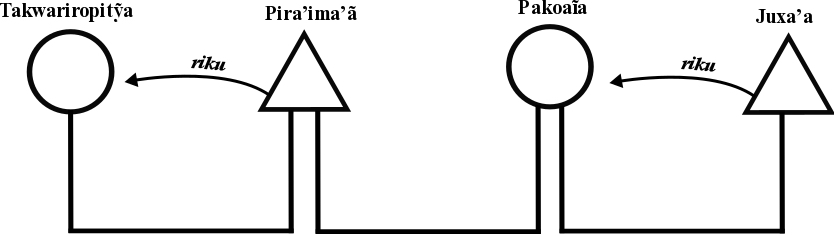
\includegraphics[width=\textwidth]{./imgs/Figura_12}
% %\caption{}
% \end{figure}

%\includegraphics[width=6.25903in,height=1.77778in]{media/image2.jpeg}

%Figura 12

Enquanto Pira'ima'ã ``pega'', \textit{pyhy}, e ``cria'', \textit{riku}, uma nova
esposa, o solteiro Juxa'a, que já havia participado da concepção da
segunda filha de Pira'ima'ã, passa a ser o segundo marido de Pakwa'ĩa;
ao passo que a jovem, e outrora \textit{mihua}, Takwariropitỹa passará a
frequentar a casa de Pira'ima'ã para, a partir de uma boa alimentação,
se transformar em \textit{imirikoa} e consequentemente, \textit{awatea}.
Mesmo esse não sendo um caso de rapto de esposa, nele encontramos algo
semelhante ao fenômeno, a saber, a possibilidade de incorporação por
meio do casamento de uma jovem esposa que ainda não é totalmente humana, 
\textit{awatea}, mas, ao contrário, estrangeira, \textit{mihua}. Se o
\textit{riku} é o mais próximo que podemos chamar de conjugalidade, essa
forma é extremamente eficiente para transformar estrangeiras, \textit{mihua}, 
em mulheres próximas, \textit{imirikoa}, ao anular as
distâncias por meio do amansamento: rapto, amansamento e casamento podem
aparecer de forma complementar.

Em níveis censitários, os raptos ocorriam com muita frequência antes do
contato, quando os diferentes grupos locais mantinham pouca ou nenhuma
relação entre si. Atualmente, o tema do rapto, \textit{hamirikoa pyhy},``apanhar mulher'', 
está relacionado fundamentalmente aos estrangeiros
\textit{mihua}. E tais mulheres são bastante cobiçadas, como também já
mencionei. Mesmo assim, na vida cotidiana, o verbo \textit{pyhy}, ``pegar'',
também pode ser utilizado como sinônimo de ``casar'', no lugar do muito
utilizado \textit{riku}. Diversas foram as vezes em que, ao questionarem
se eu tinha informações sobre os tais \textit{mihua} (os Guajá
``isolados''), os rapazes jovens se gabavam (a mim) de que, caso
encontrassem as jovens desses grupos, as levariam para casa e as
manteriam presas, agarradas ao corpo, dentro de suas redes, mantendo-as
juntas a si, \textit{pyry}, pelo tempo que fosse necessário. Isso seria
necessário por dois motivos: primeiro, para que ela não fugisse de volta para
floresta; depois, para que, bem junta ao homem, se acostumassem um com o
outro. Se uma aproximação dessa qualidade ocorrer (a jovem permanecer
agarrada ao corpo do marido por muitos dias), ela permanecerá esposa
durante muitos anos. Essa é uma ideia muito difundida entre os Guajá,
que estabelecem uma relação direta ao fato de manter-se junto à alguém, 
\textit{pyry}\footnote{O termo \textit{pyry} funciona com uma ``posposição
  adessiva'' (que exprime adjacência), podendo ser traduzido como ``junto
  a'' ou como ``para junto de'', como nos exemplos: \textit{ipyry} -- ``junto
  dele''; \textit{hapyry} -- ``junto a mim'' (Magalhães \textit{op.\,cit}., p.\,56).} como
essencial para que ocorra uma boa relação, seja ela qual for
(paternidade, casamento, e mesmo criação de animais). Vejamos um
exemplo.

Após ser atacada por uma jararaca, a cadela de Ajruhua morreu,
provocando uma grande tristeza em sua dona. Semanas depois, para suprir
a perda da finada cadela caçadora, a mulher conseguiu, por intermédio de
um jovem ribeirinho chamado Chico,\footnote{Chico do Cajú, que nasceu às
  margens do rio Caru, é um jovem de 25 anos muito querido pelos Guajá.
  É contratado da Funai para ajudar em tarefas pesadas do Posto
  Indígena, como a construção de barracões, abertura de roças, limpezas
  de pomar, dentre outras.} um filhote de vira-lata como animal de
criação, \textit{nima}, e que, com o tempo, poderia ajudá-la nas caçadas
de sua família. O pequeno filhote logo já circulava pela aldeia e, como
todo xerimbabo em seus dias iniciais, era a principal distração de todas
as crianças, motivo de orgulho e cuidado dos adultos, principalmente de
sua dona, que ficara muito feliz como seu novo cãozinho. Como eu passava
boa parte dos meus dias de aldeia deitado em qualquer rede que houvesse
disponível na casa de Wirahoa e Ajruhua, inevitavelmente tive aquele
cãozinho comendo as pontas do meu chinelo e lambendo meus dedos sujos de
terra. A todo momento, uma criança colocava o animal no meu colo para
que eu o acariciasse e mesmo brincasse com ele. Devo ressaltar que a
minha convivência com os cães da aldeia Juriti nunca foi das melhores.
Dos vários ataques que sofri --- todos repentinamente ---, uma forte mordida
me deixou sem andar durante pouco mais de uma semana, o que quase me
tirou do campo devido à profundidade da ferida (cuja cicatriz na perna
carregarei durante muitos anos).

É certo que aquele simpático filhote não representava uma grande ameaça,
por isso muitas pessoas puseram-no em meu colo, a fim de que se
acostumasse comigo, pois quase sempre as crianças se lembravam, em tom
zombeteiro, da mordida que eu havia levado. O jovem Kaawi'ia alertou-me
para o fato de que, caso o cachorrinho permanecesse um tempo sob os meus
cuidados, se acostumaria com a minha presença e, tão logo crescesse, não
me atacaria, tal como fizera seu predecessor. Devido a meus cuidados, o
animal me tomaria como mais um \textit{jara}, um ``dono''. Argumento não
muito diferente do que \textit{nós} utilizamos para nossos animais
domésticos, focos de cuidado e ``atitudes rituais'', como os gatos e
cachorros (para evocar o célebre artigo de Leach, 1983, p.\,174). Por
isso, respondi a Kaawi'ia que minha aproximação com o cachorrinho não
serviria de muita coisa, uma vez que eu não acompanharia seu crescimento
de perto e, inevitavelmente, o animal se esqueceria de mim. Foi nesse
momento que Kaawi'ia me forneceu uma informação relativamente simples,
que até agora parece basilar para entendermos os processos de
transformação de pessoas Guajá. Explico.

Segundo o jovem --- de maneira diferente da relação que os \textit{brancos}
mantêm com seus seres criados, perfilhados e estimados, sejam humanos
(filhos, por exemplo) ou não (animais de estimação, por exemplo) ---,
independentemente do tempo que eu passasse longe do cachorrinho, o fato
de o filhote me cheirar e me reconhecer nesses seus primeiros dias de
infância faria com que ele não se zangasse comigo em sua idade adulta.
Além disso, e segundo essa ideia, os ataques dos cachorros da aldeia a
mim não estavam associados a eu ser um estranho (isso também conta),
mas, principalmente, por eu não ter mantido contato com eles enquanto
filhotes; e agora já era tarde demais. Mesmo que os animais adultos se
acostumassem comigo, nada os impediria de, de uma hora para outra, me
estranharem e atacarem, como fizeram outras vezes. Se o filhote de
cachorro me reconhecesse naqueles seus primeiros meses de infância
enquanto um \textit{jara}, ele não me morderia nem se zangaria comigo na
idade adulta, mesmo eu ficando anos sem voltar para a aldeia. O
importante, ao que parece, seria esse primeiro contato, ainda quando o
ser é um filhote. Kaawi'ia afirmou-me que não se trata de esquecer ou
lembrar, \textit{imahare} ou \textit{imarakwa}, mas que a convivência é
facilitada a partir desses encontros na fase pré-matura de cada ser,
seja um animal de criação ou --- como vimos acima --- uma esposa. Certamente
não tenho a intenção de extrair de um registro pequeno princípios
sociológicos amplos, pois não estou seguro de que a explicação seja
essa.

Na mesma direção de ``reconhecer'' e ``lembrar'', eram dirigidos a mim
comentários como: mais cedo ou mais tarde, eu precisaria retornar a
minha casa em São Paulo, pois minha família estaria com saudades; ou que
minha mulher se casaria novamente; e mesmo, que meu sogro se zangaria
comigo.\footnote{Comentários semelhantes a tantos outros, que os
  etnógrafos descrevem ao explicar o desconforto moral aludido por seus
  interlocutores por estarem sozinhos no campo.} Embora nestes
comentários a ideia de esquecimento, \textit{imahare}, nunca estivesse
presente, o problema era sempre a noção de uma dolorida lembrança, \textit{imarakwa},\footnote{Fato curioso, que ainda estou para entender,
  ocorria toda vez que eu espirrava. Após um espirro, quem estivesse por
  perto comentava comigo, e com todos em volta, em tom de brincadeira,
  que meu espirro era um sintoma de saudades de minha esposa, pois
  quando se pensa muito em alguém sente-se vontade de espirrar.} que
poderia me deixar triste e me adoecer. Nesses casos, as ideias de
\textit{pyry}, ``junto a'', ``para junto de'', e \textit{riku}, ``estar junto em
movimento'' e/\,ou ``produzindo uma ação'', parecem centrais ao informarem
tanto o rapto de mulheres quanto a captura de animais.

\textit{Pyry}, ``estar junto'' ou ``estar próximo'', é uma categoria que
revela muito da socialidade Guajá, sendo ela mesma a condição do
\textit{riku}. O \textit{pyry} complementa a noção expressa por \textit{riku}:
\textit{riku pyry}, ``criar junto a''. O próprio termo de cognação que
exprimiria, em linhas gerais, a ``consanguinidade'', \textit{harapihiara}
``meu consanguíneo''\textit{,} pode ter se originado linguisticamente da
nominalização da posposição \textit{pyry}, traduzido literalmente em sua
origem por ``o que está junto de mim'', pois, como sabemos, para diversos
casos amazônicos a ``consanguinidade'' nada mais é do que uma
ultraproximidade cognática. No entanto, esse termo descritivo, pelo seu
extenso uso como de cognação, teria se lexicalizado e se tornado uma
palavra hoje não segmentável em seus morfemas constitutivos. A
nominalização da posposição \textit{pyry} é realizada atualmente na língua
guajá por meio da palavra \textit{hapyryhara}, ``aquilo'' ou ``aquele/\,a que está
junto a mim''.\footnote{\textit{Ha} mais \textit{pyry} mais
\textit{har} mais \textit{a} é igual a \textit{meu} mais \textit{junto a} mais sufixo nominalizador
{har} mais sufixo nominal \textit{a} igual a \textit{aquilo}, \textit{aquele/\,a que
está junto a mim}.} Assim, de acordo com Magalhães (comentário
pessoal), \textit{harapihiara} teria se especializado como termo de
cognação, enquanto \textit{hapyryhara} é o atual termo descritivo para
qualquer objeto que esteja junto a algo ou alguém (uma sacola que esteja
junto a mim, por exemplo).

Desta forma, todas as relações do tipo \textit{riku} são ditas como
aquelas estabelecidas entre seres que se reconhecem como
\textit{harapihiara}. Todo ser dito \textit{nima} é \textit{harapihiara} de
seu \textit{jara}, e vice-versa. Esse tópico é discutido também por
Cormier ao demonstrar que a relação entre uma mulher e seus animais de
estimação (os macacos, mais especificamente) ocorre entre consanguíneos
--- \textit{harypihary}, em sua grafia ---, pelo fato de os macaquinhos serem os
xerimbabos (\textit{hanima}, em sua grafia) das mulheres. Todas as sete
espécies de macacos conhecidos pelos Guajá são tomadas como xerimbabos, 
\textit{pets}: macaco-capelão; macaco-prego; cairara; sagui
\textit{atamaria}; cuxiú; macaco-da-noite e macaco mão-de-ouro. Este
último, em pouquíssima incidência na região do rio Caru. Cormier ainda
ressalta que todos os \textit{pets} são chamados \textit{hanima} e que os
macaquinhos são aludidos pelo termo \textit{hamymyra}, ``minha criança'', o
mesmo utilizado pelas mulheres ao se referir a sua prole em geral (\textit{op.
cit.}, p.\,115). A autora argumenta que, embora toda ``vida da floresta''
(\textit{forest} \textit{life}) seja considerada um ``parente'' (\textit{kin}),
os macacos de estimação são incorporados mais diretamente ao sistema de
parentesco, sobretudo no nível doméstico. Segundo Cormier,
diferentemente de outros animais, os filhotes de algumas espécies de
primatas podem, após ``incorporados'' a uma família, receber nomes
próprios e apelidos que denotariam parentesco como: ``papai avermelhado'',
para um capelão;\footnote{Embora a autora não explique, um apelido como
  esse provavelmente está relacionado à vermelhidão presente nas
  extremidades de seus membros e rabo.} ``irmã'' ou ``filha'', para um
macaco-cuxiú (fêmea, imagino); ``cunhadinho'' para um macaco-da-noite; e
``marido do sagui'', para o sagui \textit{atamaria} (Cormier, 2003, p.\,115).

O próprio morfema \textit{xa'a}, como vimos no sistema de nomes, também
pode ser estendido aos macacos de estimação. Então, por exemplo, a dona
de um capelão, animais chamados ``\textit{wari}'', poderá chamá-lo de
``\textit{warixa'a}'', meu ``guaribinha'', ou meu ``capelão parente''. Por
isso, traçar relações de parentesco entre os diversos animais domésticos
é algo que pode acontecer (em tom de brincadeira) nas aldeias, e os
termos \textit{hapihiara}, ``irmão'', \textit{imena}, ``esposo'',
\textit{hamirikoa}, ``esposa'', \textit{imymyra}, \textit{taira} e
\textit{tajyra}, ``filhos dele'' ou ``dela'', a depender do sexo dos pais e do
falante, são acionados a todo tempo, a fim de demarcar relações
específicas entre animais. A forma particular de domesticação desses
macacos encontrada por Cormier, cuja relação de parentesco é tida como
central ao seu trabalho, denota menos uma ``proximidade de natureza entre
humanos e animais'', como defende a autora, mas sim, outra forma de
relação que postula certas homologias relacionais. Se pensarmos junto
com a ideia de \textit{riku}, a citada nominação dos macacos fará parte de
um sistema de classificação que recusaria o par natureza e sociedade,
uma vez que ``a natureza e a sociedade não são neste caso separadas por
fronteiras ontológicas'' (Descola, 1992, p.\,116).

Como exemplo, o sagui, \textit{atamaria}, de Panyxĩa era mantido preso
pelo pescoço, amarrado a uma viga de sua casa. Sua dona o mantinha assim
por o animal ser \textit{imahy}, ``nervoso'', ``raivoso'', ``brabo'', e fugir
constantemente para encontrar o sagui de sua avó, Amỹ Piirawãja. Ambos
eram machos e quando se encontravam gritavam muito e reviravam os
objetos. Segundo Panaxĩa, o sagui de Amỹ Piirawãja e o seu eram
\textit{harapihiara} entre si, por isso permaneciam juntos para
\textit{wata}, ``caminhar'', ``caçar'', ``coletar''; \textit{wata} \textit{pyry}, ``andar
junto'', para ser mais preciso. Quando lhe perguntei se quando sem sua
coleira o sagui não fugiria para a floresta para encontrar outros
cognatos, \textit{harapihiara}, disse-me que os saguis da floresta eram
\textit{mihua}, ``selvagens'', para seu sagui, portanto, só seriam
\textit{harapihiara} os saguis que viviam naquela aldeia. Isto sugere que,
tal como as relações de parentesco, a relação entre dois animais só pode
ser traçada a partir da que cada um estabelece em seu mundo. Mesmo os
termos de parentesco ``transpostos'' para as relações animais, tal como
vimos no exemplo de Cormier linhas acima, são dirigidos de acordo com o
caso, e não há uma regra absoluta que prescreva substância e forma. Em
outras palavras, cada xerimbabo será parente de outro de acordo com a
espécie, a história, a forma de domesticação, o humor de sua dona, e
outros detalhes.

Ainda no caso dos animais de criação, como em outros povos da América do
Sul (Vander Velden, 2012, pp.\,112--117), ao chegar nas aldeias os animais
quase sempre são modificados. Aves têm parte de suas penas retiradas ou
aparadas para que não consigam fugir, bem como as pontas seus bicos são
cortados com tesouras para que, ao bicarem, não machuquem sobretudo as
crianças. As afiadas garras de quatis são retiradas ou lixadas com lima.
Paquinhas e filhotes de cotias têm seus dentes serrados (também com
lima) para que as pontas cortantes não firam ninguém. Queixadas e
caititus devem ficar bem amarrados ou presos em currais, para que o
corre-corre dos bichos não transforme a aldeia em uma grande bagunça e
gritaria; esses animais comem tudo o que encontram pela frente, de lixo
a pintinhos. Apenas os macacos parecem não sofrer tantas intervenções,
como cortes e outras injúrias. Com os macacos nada se faz. Quando muito,
são presos com cordinhas por algum tempo, até ficarem mansos. Os que
nunca se acalmam permanecerão amarrados até um dia em que serão soltos.
Não basta, portanto, \textit{estar junto}, é preciso que essa proximidade não
cause danos.\looseness=-1

%\textbf{Foto do quati sendo mexido}
%\begin{figure}[!ht]
%\centering
 % 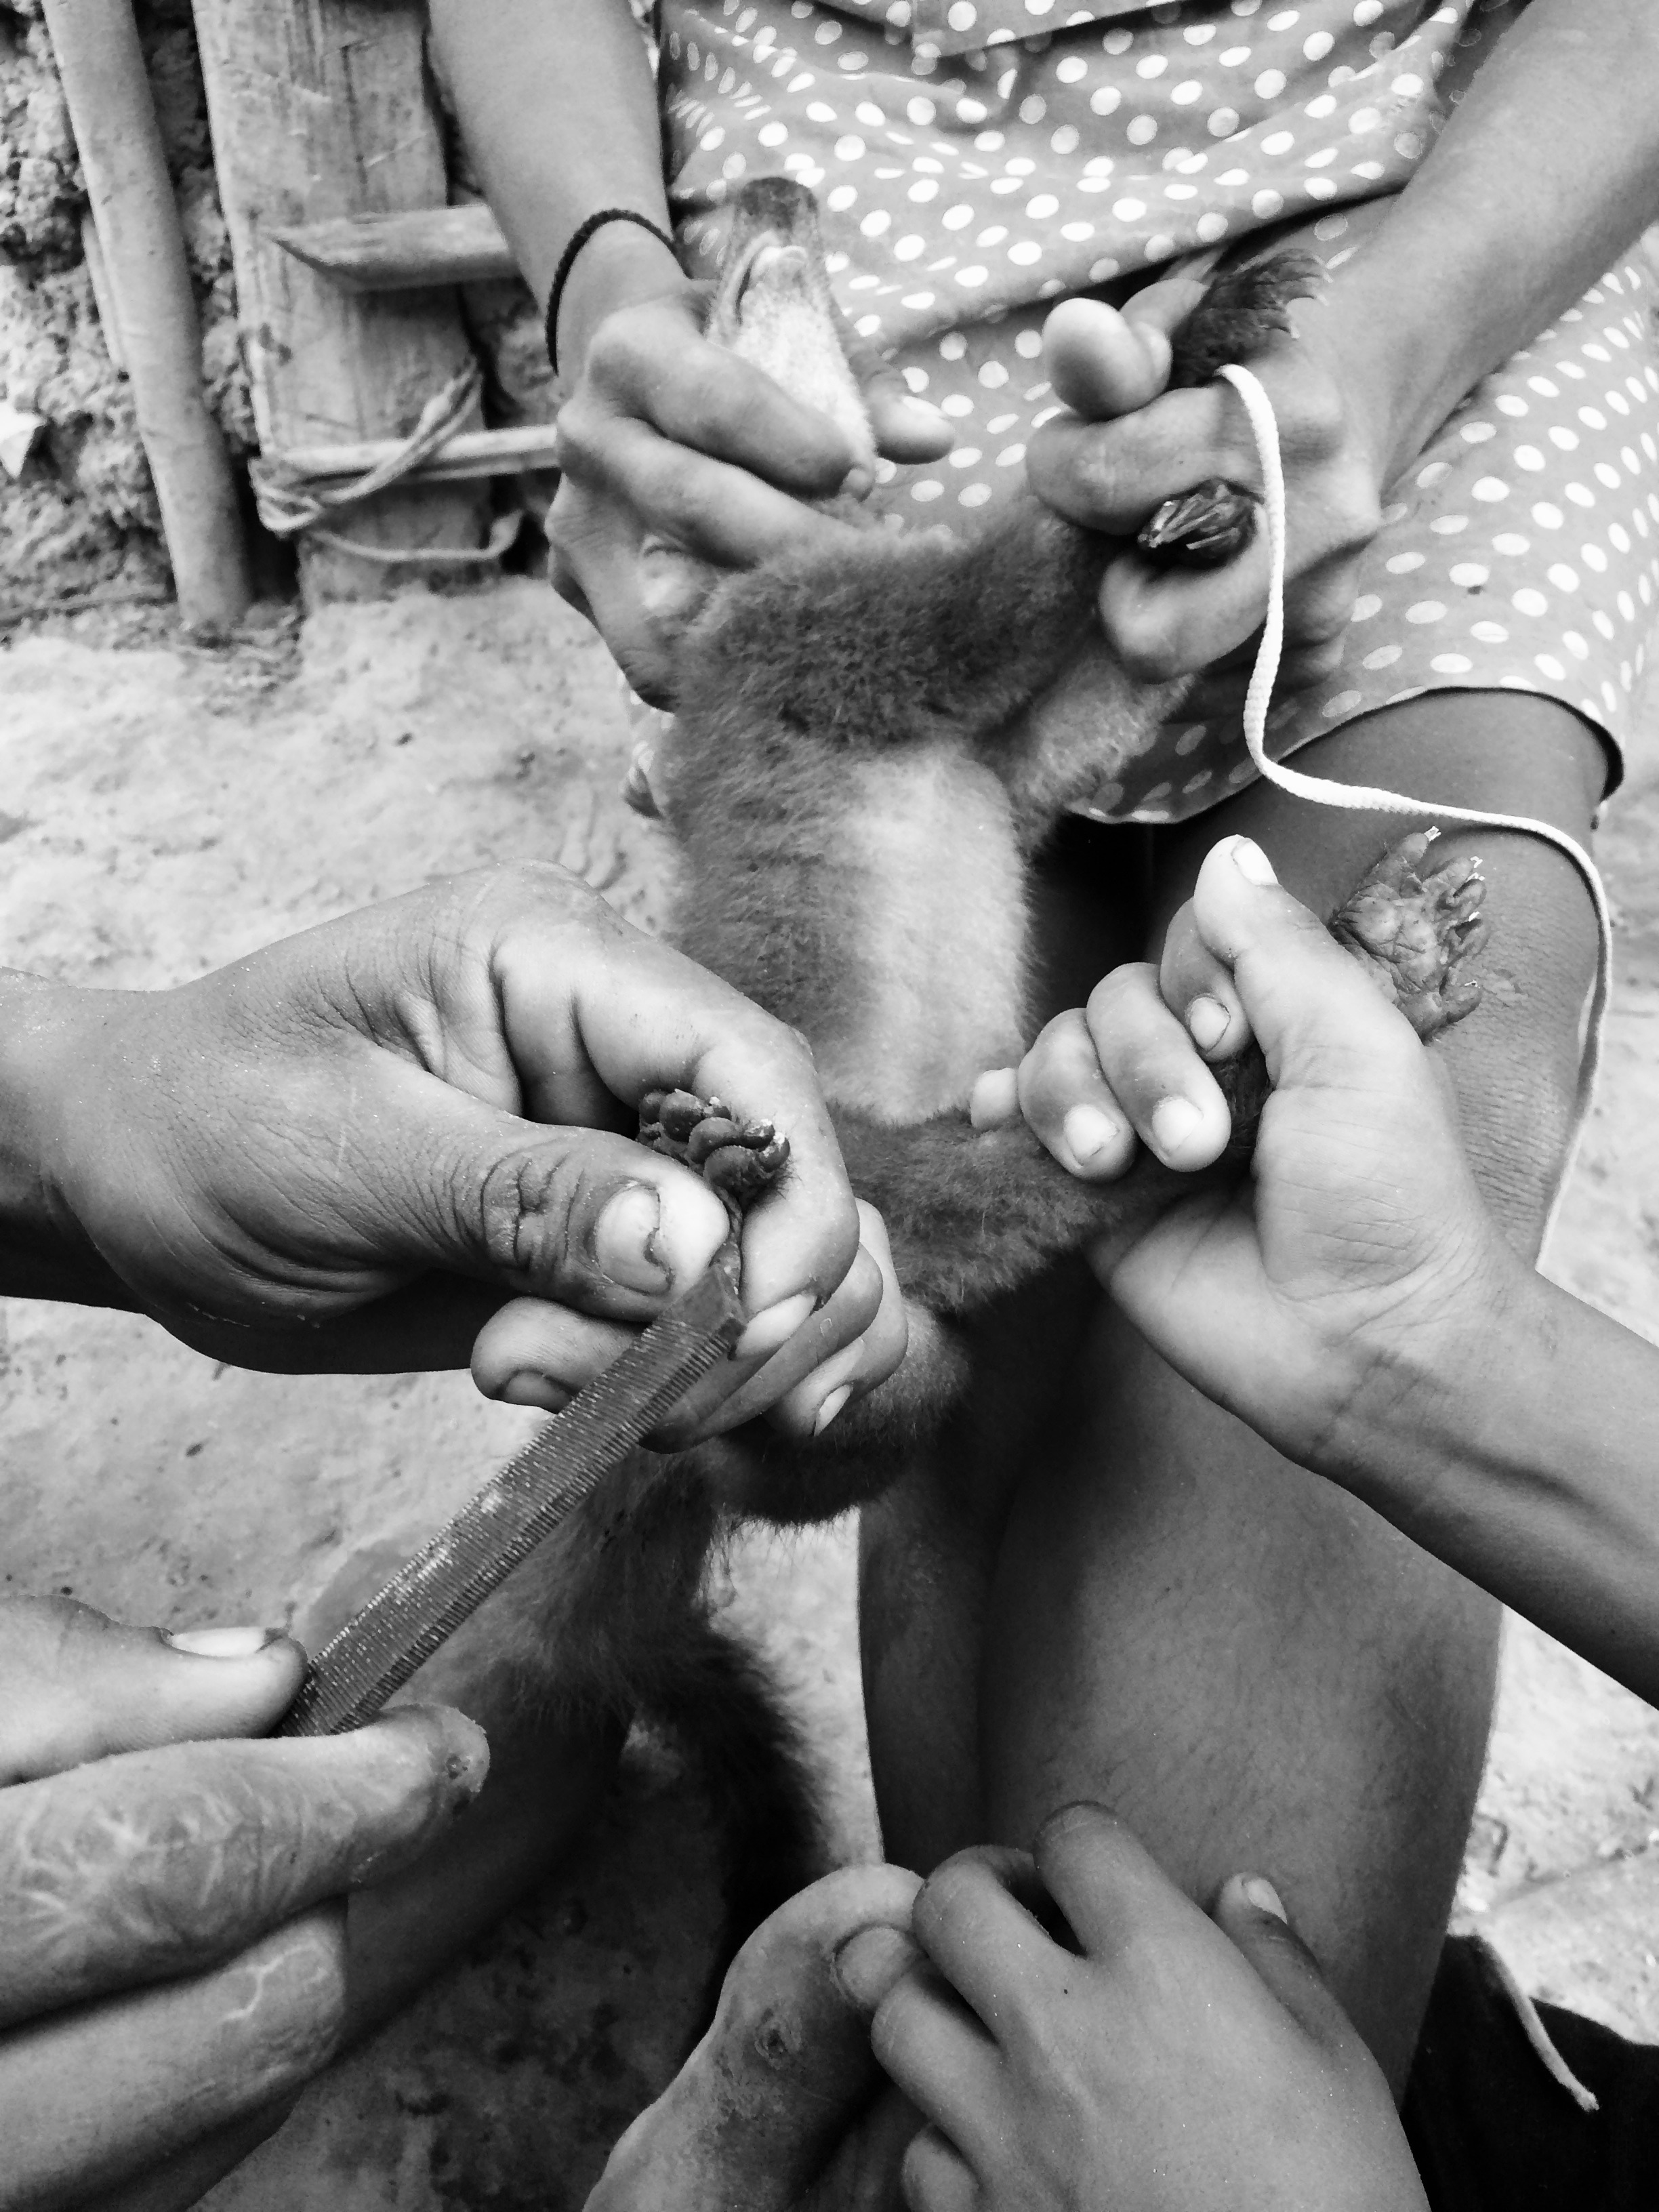
\includegraphics[width=\textwidth]{./imgs/IMG_0343}
%\caption{As unhas afiadas do quati de Xikapiõ precisam ser limadas para não ferir a sua dona (aldeia Juriti, 2016).}
%\end{figure}

A vida desses animais na aldeia depende de, digamos, acordos
interespecíficos entre seus donos humanos e essas criaturas. De maneira
geral, a primeira reação dos animais é resistir à criação, e muitos
conseguem fazê-lo, escapando ou morrendo, causando frustração naquelas
que desejavam ser donas, \textit{jara}, criadoras. Os animais têm medo
quando chegam à aldeia e muitos simplesmente não querem comer, morrendo
também de fome. Animais como o jacaré, por exemplo, são difíceis de
domesticar sobretudo diante de sua dieta exclusivamente carnívora, às
vezes complicada para ser administrada pelos humanos. O último jacaré
capturado que vi em uma aldeia recusou as carnes de caititu e cotia
que lhe eram oferecidas e morreu por inanição.\footnote{A outra opção
  seria deixá-lo se alimentar à noite, com sapos e outros animais que
  lhe apetecem, mas isso estava fora de questão por motivos
  autoevidentes. Ninguém deixaria um jacaré solto na aldeia à noite.}
Não apenas o jacaré em questão, mas diversos macacos, aves como
periquitos, araras, inhambus, e mamíferos como pacas e cotias, durante
os primeiros dias da nova vida se opõem à mudança na dieta. Notem que
para cada animal, ou conjunto de animais, algumas regras são obedecidas.
Algumas espécies comem farinha, outras não. Mingaus, carnes, frutos, e
até refeições como as humanas, cada um dos alimentos vai variar de
acordo com os hábitos da espécie. Para alguns a comida de gente, 
\textit{awa nimi'ua}, bastará, para outros a alimentação será mais
seletiva e específica.\looseness=-1

Os animais da aldeia precisam aprender a ser animais de aldeia, e nem
todos estão dispostos a isso. Existem diversas maneiras dos bichos
resistirem, fugirem ou sabotarem a nova vida de cativos. Os filhotes de
cotias podem roer as cordas que lhe prendem e fogem de volta para a
floresta. Os quatis são muito bravos e podem ser violentos com as
crianças. Além disso, comem os pintinhos que vivem soltos na aldeia, e
podem roubar ovos de galinhas e de outras aves como o jacu. Esses quatis
de criação também são um problema dentro de casa pois mexem em toda a
comida, furam os sacos e espalham farinha por todos os lados. Assim como
os quatis, os filhotes de porcos também querem comer pintinhos da aldeia
e, por serem fortes, quase incontroláveis em sua corrida, precisam viver
em currais, \textit{hakãnã'ã}. ``Os porcos até parecem gaviões'', me
disse um amigo certa vez, dada a avidez dos queixadas por pintinhos. Os
macacos-prego são muito bravos, ao mesmo tempo que habilidosos, uma
combinação que não tem como dar certo. Mexem em machados, facas, cordas
e até moto-serras. São eles os mais ciumentos e atacam os filhos de suas
donas. Os macacos-cairara, por sua vez, adoram ficar brincando e são
sempre comparados às crianças. Os macacos cuxiú-preto são grandes
companheiros de caminhada, calmos, são capazes de manter uma grande
conexão com suas donas nas caminhadas. Os Guajá sempre lembram como os
cuxiú são bons companheiros de caçada. Um dos animais mais exigentes é o
capelão. Sua domesticação sempre será difícil pois se negam a comer
qualquer alimento relacionado à dieta humana, além de serem ``chorões''
--- \textit{já'ohara}, ``chorador'' --- e terem muita ``saudade''
--- \textit{imarakwa}, ``pensar'' --- da vida na mata. Os capelães morrem muito
facilmente na aldeia. É uma tarefa difícil criá-los. Não comem farinha,
milho ou arroz, e nem mesmo as frutas dos novos pomares (plantados com a
ajuda de não indígenas) como manga e jaca. Os capelães só gostam da
comida do mato.

\section{familiarização, criação}

Um modelo elaborado para a Amazônia a respeito das relações entre
``donos'' --- ou ``senhores'' --- e ``criaturas''  --- ou ``xerimbabos'' --- 
foi o que Fausto denominou ``Predação Familiarizante''. A partir da relação entre os
humanos e seus xerimbabos oníricos, que auxiliam os primeiros em suas
curas, Fausto observa um aspecto fundamental da socialidade ameríndia, a
saber, as ``relações assimétricas de controle, real ou simbólico,
conceitualizadas como formas de adoção'' e pertinentes a quatro domínios:
caça, xamanismo, ritual e guerra (Fausto, 2001, p.\,413). Não vou
discutir em detalhes o modelo do autor, uma vez que, além de ser de uma
ambição generalista, foi retomado de forma comparativa em um importante
artigo (Fausto, 2008).\footnote{O modelo de Fausto dialoga diretamente
  com a ideia de ``economia simbólica da predação'', tal como desenvolvido
  por Viveiros de Castro. Assim formula o autor: ``Em resumo, se de fato
      é possível falar em uma economia simbólica da predação (Viveiros de
      Castro, 1993), é preciso desenvolver seu complemento --- que não é uma
      teoria da reciprocidade equilibrada, mas sim das relações assimétricas
      do tipo pai-filho ou sogro-genro, constituídas por meio do homicídio e
      do sonho-transe. A predação é um momento do processo de produção de
      pessoas do qual a familiarização é outro. Não se compreenderá o
      sentido da guerra ameríndia por sua redução às relações simétricas de
      troca, mas sim, pela construção de um \textit{modelo das relações
      assimétricas de controle simbólico}'' (Fausto, 2001, p.\,418).} Ao apresentar ``a operação de aquisição do poder xamânico
    como um processo de familiarização de entes extra-humanos, com
    frequência associados à predação e ao canibalismo'', o autor nota que ``a
        relação familiar é modelada por duas relações assimétricas que envolvem
        controle e proteção: aquela entre pai e filho e/\,ou aquela entre dono e
        bicho de estimação'' (Fausto, 2001, pp.\,415--416). Das formas que preveem o
esquema da familiarização além dessas duas restariam: o controle
simbólico sobre objetos rituais e ornamentos corporais (Ikpeng, Tukano);
a dessubstanciação de animais caçados a fim de lhes retirar as armas
(Makuna); os cativos de guerra (Tupinambá) e crianças raptadas (Ikpeng,
Curripaco), tratados como xerimbabos; e, por fim, o processo de
apropriação, ou domesticação, do espírito de uma vítima, ou presa, humana pelo seu
carrasco, como ocorre em diversos povos (como os Araweté, Nivacle, Wari).\footnote{\textit{Idem}, p.\,417.}
A doutrina dos cantos de cura \textit{karahiwa}, dados
pelos \textit{akwawa} (inimigos oníricos que auxiliam o xamã), entre os
Parakanã, ``ou a ideia de alteração (devir-outro) do matador araweté''
prescrevem um ordenamento semelhante entre as operações de domesticação
no xamanismo e na guerra; e ``ambas são parte de uma economia
generalizada de produção de pessoas'' (Fausto, \textit{op.\,cit}., pp.\,417--418). Tal
como no \textit{riku} guajá:

\begin{quote}
Os temas principais são ontológicos: aquisição de alma e virtualidades
de pessoas, nominação e existência, desenvolvimento das capacidades
plenas da pessoa e maturação, controle sobre os processos mórbidos e
longevidade, conquista sobre a morte e imortalidade.\footnote{\textit{Idem}.}
\end{quote}

Fausto utiliza o modelo da relação entre senhores e xerimbabos, que
prescreve um vínculo de proteção e adoção, como constituinte de um tipo
de socialidade particular encontrada em diversos grupos amazônicos, mais
especificamente, no xamanismo Parakanã. Tal modelo, denominado
``predação familiarizante'', atesta de forma bem sucedida que as
diversas relações, sejam entre matador e vítima pós-homicídio ou entre
xamãs e espíritos auxiliares (dentre outras), são pensadas como uma
forma de ``filiação adotiva'':

\begin{quote}
A relação prototípica de controle nas sociedades ameríndias não é,
porém, a do mestre e do escravo, mas a do senhor e do xerimbabo, que é
exercida praticamente na familiarização de animais e no rapto de
crianças estrangeiras. Estes, porém, não são senão casos particulares de
uma estrutura relacional mais ampla, que envolve a familiarização do
princípio vital da vítima na guerra e de espíritos de animais no
xamanismo.\footnote{Fausto, 2001, p.\,539.}
\end{quote}

O autor não menciona a relação marido-esposa em seu primeiro esquema
(2001) relacional, diferentemente do que encontrei entre os Guajá
(embora, talvez não seja por acaso o modelo da predação familiarizante
surgir a partir de uma sociedade que prescreve justamente o casamento
com \textsc{zd}). No entanto, em uma análise mais recente Fausto insere a
``maternidade'' e a ``matrimonialidade'' no artigo em que retomou as ideias
de ``maestria'' e ``domínio'' como fundamentais à compreensão das
socialidades amazônicas (Fausto, 2008). Para o autor, a ``maternidade'' é
tratada como um caso particular das relações de maestria e ``se expressa
nas figuras da mãe da caça (ou de alguma espécie em particular) ou da
mãe de plantas (em especial, as alucinógenas). Contudo, o uso da
categoria `mãe' para designar entidades similares aos donos é restrita
etnograficamente, além de não se aplicar ao espectro mais geral de
relações de domínio que caracterizam a noção de dono-mestre'' (Fausto,
2008, p.\,350).

O caso Guajá questiona o ``absolutismo'' das formas \textit{dono-mestre} ---
sugerindo uma multiplicidade de formas que não se sobrepõem --- e concebe
a maternidade (fisiológica) a partir de um modelo onde o que prevalece é
a relação \textit{riku}, que nem sempre será uma relação assimétrica de
``controle simbólico'' (Fausto, 2001, p.\,418). Em outra palavras, toda
relação \textit{riku} estabelecida entre um \textit{jara} e um \textit{nima}
é, sim, assimétrica, da mesma forma que Fausto pensa as relações de
maestria; porém nem sempre o que estará em jogo será domínio e controle.
Por exemplo, a relação entre um \textit{karawara} dito ser, no céu,
\textit{jara} de determinado animal terreno, como o \textit{Makaro}
\textit{Jara} (gente-pomba-galega) e seu correlato terreno, não é uma
relação de controle. As qualidades desse \textit{karawara} estão
relacionadas ao fato de ele ser um exímio caçador de porcos (como
veremos no último capítulo) e não por controlar as pombas-galegas
(\textit{Patagioenas cayennensis}) terrenas. Dessas últimas, o
\textit{Makaro Jara} é apenas uma ``versão celeste'' ou ``duplo'', como venho
chamando aqui. Ainda assim, as pombas-galegas, \textit{makaro}, terrenas
são ditas \textit{nima} de \textit{Makaro Jara}, mesmo não sendo controladas
por esse. Isso sugere que o \textit{riku} relaciona seres sem
necessariamente produzir uma relação de poder, domínio ou controle, mas
sim, de assimetria, tendo-se em vista que o \textit{Makaro Jara} é humano,
e o \textit{makaro} terreno não. E as versões humanas, ou que pelo menos
se consideram como tal, são as que se veem como \textit{jara}.\looseness=-1

Fausto observa que o conceito de \textit{maestria} ``é tão central à
compreensão das sociocosmologias indígenas quanto a afinidade'' (Fausto,
2008, p.\,330). No caso Guajá, parece-me que ``maestria'' e ``afinidade''
(no sentido de ideias que determinam o casamento, em uma teoria da
relacionalidade generalizada, nas palavras de Viveiros de Castro, 2002)
não podem ser pensadas isoladamente. E quanto à aliança especificamente,
ela é para os Guajá uma forma de ``maestria'', \textit{riku}. Ao apontarem
que casar é \textit{riku} (ação que está em vários lugares, produzindo
afecções entre seres de diferentes ordens, inclusive entre um homem e a
filha de sua irmã, \textsc{zd}), os Guajá asseveram que a aliança é um caso
particular da maestria. Se a intenção é justamente ``fazer parentesco
querer dizer outra coisa'', as ideias Guajá para o casamento ``não só
determinam outros referentes que os nossos, como envolvem outros
componentes'' (Viveiros de Castro, 2002, p.\,407).

Quanto à ``matrimonialidade'' (nas palavras de Fausto), o autor a sugere a
partir da perspectiva do xamanismo, ``pois o xamã constitui verdadeiras
famílias espirituais: tem uma esposa, afins e gera filhos-espíritos''
(Fausto, 2008, p.\,351). E, a partir do exemplo Nambikwara-Mamaindê, traça
uma relação entre ``matrimonialidade'' e ``familiarização'':

\begin{quote}
Os Nambikwara-Mamaindê nos fornecem o exemplo mais sugestivo dessa
assimilação entre casamento e familiarização (Fausto, 2001b). A
esposa-espírito, que é um jaguar, é denominada da \textit{mãindu}, ``minha
criação'' ou ``meu xerimbabo'', pelo marido-xamã. Como era de se
esperar, observa-se também aqui a instabilidade posicional que marca, em
geral, as relações de mútua constituição entre xamãs e auxiliares: ``não
se sabe ao certo quem está `criando' quem. Embora o xamã chame a
mulher-espírito de `minha criação'; ao partilhar comida e enfeites
corporais com ela, o xamã indica que é ele quem está sendo `criado' por
ela''.\footnote{Miller, 2007, p.\,199; Fausto, 2008.}\looseness=-1
\end{quote}

De fato, o exemplo acima é rico ao apontar um mecanismo que, se
cosmopolítico para os Nambikwara-Mamaindê, para os Guajá está no plano
da sociologia (embora, como ainda veremos, casamentos com mulheres
celestes também podem ocorrer), em que as esposas são tidas literalmente
como ``minha criação'' ou, em uma tradução literal, ``objetos do meu criar'',
\textit{imirikoa}. E se a cosmologia mamaindê propõe uma recíproca na
relação de ``criação'' entre maridos-xamãs e esposas-espíritos, a
sociologia Guajá --- bem como a Tupinambá, como vimos acima --- também
defende que maridos ``criam'' esposas, esposas ``criam'' maridos.

Uma mulher mais velha, muitas vezes, viúva, pode propor casamento a um
jovem promissor da mesma forma que os homens fazem com as mulheres:
\textit{jaha ariku ta ni pyry}, ``eu quero ficar com você'', ou ``te criar''. Foi
assim, inclusive, que Ajruhua e Wirahoa se casaram, ela com 24 e ele com
16 anos. Um casamento recorrente nos padrões Guajá, em que mulheres
adultas com 25, 30 desposam rapazes jovens de 14, 15 anos. Por um lado,
esse e outros arranjos são concomitantes ao contato, momento em que
historicamente os Guajá foram dizimados e sofreram uma drástica
depopulação, o que inflete diretamente nos arranjos matrimoniais
--- incesto, mudanças no padrão residencial, poligamia onde não havia,
etc. A literatura etnológica está repleta de exemplos como esse.\footnote{Para
dois casos tupi-guarani, ver Müller, 1993; e Wagley, 1988.} Mas recorrer
ao argumento da crise do contato esconde as próprias preferências das
pessoas. Diz-se das mulheres ``criarem'' seus maridos, porém o argumento
não me foi fornecido com todos os detalhes que adquiri do casamento a
partir do ponto de vista masculino. O fato de eu ser homem não deixou
que eu apreendesse com apuro o \textit{riku}, ``casamento'', tal como as
mulheres o mantêm com seus homens. Por outro lado, os efeitos dessas
criações (de mulheres sobre homens), se tornam aparente todo o tempo, e
novas uniões intergeracionais são desfeitas muitas vezes antes de
começar. Não apenas os efeitos, mas novas linhas de fuga são traçadas a
cada novo arranjo. Podemos ver isso no caso de Jawa'nĩa, um jovem que
com apenas 15 anos saiu de sua aldeia de origem para ser criado pela
mulher Ximirapi na aldeia Tiracambu. Ela tinha cerca de 35 anos na
época. Uma vez na aldeia, vivendo, sendo criado por Ximirapi, o rapaz se
``acostumou'' com uma outra jovem, mais nova até do que ele, com quem
decidiu se casar, largando para trás a ``mulher velha'', voltando à sua
aldeia de origem com a jovem mulher.\footnote{Hoje em dia (2017), alguns
  anos depois, ele voltou à viver na aldeia de sua esposa.}

Podemos dizer que há uma assimetria nesta relação marido e esposa que
escapa à pura dominação masculino-feminino e instaura um tipo de
socialidade intersexual, que no plano terminológico prescreve a esposa
--- \textit{imirikoa}, ``aquela que eu crio'' --- como alguém que é resultado da
ação \textit{riku}; porém no plano da ação, apesar de não aparecer na
terminologia, homens indubitavelmente também são ``pegos'' para
``criar''. Encontramos nos Guajá tanto homens criando mulheres quanto
vice-versa. Por isso a mulher enquanto puro ser criável, e não que cria,
parece estar fundamentalmente no plano da língua, enquanto a etnografia
prefere mostrar outra coisa.

\section{a ficção do dono}

Para finalizar o capítulo, problematizo etnograficamente a discussão
sobre os ``donos'' na Amazônia; mas antes, para auxiliar na análise,
discuto alguns casos correlatos ao \textit{riku} Guajá encontrados em
povos falantes do Tupi-Guarani, particularmente. Não compete a este
trabalho avaliar os problemas e as soluções impostos a outras
etnografias; e os questionamentos e soluções que venho encontrando para
o caso Guajá não precisam ser completamente replicáveis a outros
contextos etnográficos, correlatos ou não. Porém, algumas conexões ---
ainda que parciais --- podem ser traçadas entre o caso Guajá e outros
Tupi-Guarani, uma vez que, apesar das claras diferenças entre esses
coletivos (como todos sabemos), encontramos de maneiras transversas
aspectos que dialogam.

Linguisticamente, o \textit{riku}, como um termo que exprime relações
particulares, está presente em algumas outras línguas da família
tupi-guarani, como o \textit{reko} do guarani mbya como vimos acima, ou
na formação de palavras associadas ao termo como o termo para esposa,
\textit{he-remirikó}, na língua tenetehara (Wagley e Galvão, \textit{op.\,cit}.).
Tal ideia experimentou diferentes traduções, exprimindo subjetividades
diversas, e, como observamos, as traduções linguísticas do tipo ``estar
junto a'', ``estar com'' (ou qualquer outra semelhante), no caso Guajá, não
seriam suficientes para a compreensão da relação como um todo. Meu
trabalho não é o primeiro a abordar o interesse de um povo para com essa
concepção de relação encarnada na forma \textit{riku}. O exemplo mais
relevante para o caso é a ideia de \textit{werekio}, encontrada entre os
Zo'e, um povo linguisticamente próximo aos Guajá.\footnote{Segundo
  Rodrigues, ao lado de outras línguas, tanto o guajá quanto o zo'e
  pertencem ao subgrupo \textsc{viii} (oito) da família tupi-guarani, o que os
  fazem menos distantes no plano intrafamiliar.} Havt traduz o termo
\textit{werekio} como ``estar com'' e ainda ``tomar como esposa'', e lembra
que, tal como entre os Guajá, é um termo que aparece ``com frequência em
outros contextos {[}\ldots{}{]}, não necessariamente envolvendo um matrimônio''
(Havt, 2001, p.\,48). Para a autora, ``quando um Zo'e fala em
\textit{werekio} ele está se referindo a uma adoção, no sentido de uma
incorporação daquele elemento a seu viver. Mais adiante, esse termo vai
ser encontrado referindo-se a um cônjuge, ao porte de algum utensílio,
ao uso de uma técnica de apropriação e/\,ou uso do ambiente, aos cultivos
das roças, enfim, a qualquer aspecto que possa ser definido como parte
(ou que possa fazer parte) da vida, de um jeito de ser''.\footnote{\textit{Idem}.} Tal como encontramos entre os Guajá, os Zo'e se referem a
diferentes atividades mediante um mesmo termo capaz de expressar ideias
próximas, embora diversas. Termo pelo qual são tratadas várias ações,
não por uma escassez de outros específicos a elas, mas por ser o índice
de outra propriedade relacional, isto é, sugerindo uma homologia nas
práticas. Porém, a despeito da precisão etnográfica da autora, cujo
cognato \textit{werekio} se relaciona ao cultivo das roças, à
conjugalidade, à posse de objetos, dentre outras possibilidades, Havt
prefere precisá-lo por meio de ideias pré-existentes, como ``jeito de
ser'', ou mesmo ``costume'' (Havt, \textit{op.\,cit}., pp.\,48--50, nota 36). Esses
termos, para o caso Guajá, soariam um pouco vagos, uma vez que se trata
muito mais de um sistema de ação, que relaciona e interfere na vida das
pessoas, do que um ``estado'' de vida ou um ``costume''. Segundo Havt, o
\textit{processo de amansamento}, como a incorporação de um xerimbabo, os
cultivos das roças, até a incorporação dos afins, corresidentes e os
\textit{kirahi} (os não indígenas) a um grupo local, ``guarda estreita
relação com a noção de (\textit{were})\textit{kio}'' que também faz
``referência ao tomar alguém como cônjuge''.\footnote{\textit{Idem}, p.\,65.} Para Havt, o
\textit{werekio} faz:

\begin{quote}
{[}\ldots{}{]} referência a algo que é incorporado como se fosse um hábito,
um costume. Por exemplo: faz parte do \textit{jeito de ser dos Zo'e}
portar o adorno tembetá, \textit{embepot}, feito de madeira poturu, na
região pré-labial inferior; fazer de alguém seu cônjuge efetivo é
expresso como \textit{werekio}; os cultivos atuais --- relacionados em
diversas narrativas ao contato com os vizinhos \textit{Tapãaj} que se
tornaram inimigos --- são considerados como adoções, da mesma maneira que
as flechas atuais; a adoção, possibilitada pelo contato pelos
\textit{Kirahi}, de machados com lâmina de metal também é tratada em
termos da incorporação desse utensílio ao jeito de ser zo'e.\footnote{\textit{Idem}, p.\,66.}
\end{quote}

Novamente, ideias como ``jeito de ser'', ``hábito'' e ``costume'' são
utilizadas para explicar esse conjunto de ações. Tudo se passa como se o
\textit{werekio} zo'e fosse algo dissociado das próprias ações de adotar,
plantar, portar, casar e incorporar. Como exemplo, a incorporação de
utensílios vindo do mundo dos não índios ``é tratada em termos da
incorporação desse utensílio ao jeito de ser zo'e''. No final de sua
análise, a autora sintetiza o \textit{werekio zo'e} como a ``incorporação
de algum aspecto como hábito''.\footnote{\textit{Idem}, p.\,66.} De forma diversa, o que
proponho para o caso Guajá é que não há ``jeitos de ser'', mas
\textit{formas de agir} (e outras formas de ação): incorporação, adoção,
relação de casamento, dentre outras que elenquei nos parágrafos
anteriores.

Para os grupos Guarani, os termos \textit{teko} e \textit{reko} também
foram traduzidos, em diferentes autores, a partir de ideias como ``modo
de ser'' e ``jeito de ser'' e se vinculam a ``uma outra (noção) que assume,
em grande parte das análises, uma conotação espacial forte, a de
\textit{tekoa}'', o local de exercício do \textit{teko} (Pissolato, \textit{op.\,cit}.,
pp.\,105--106):

\begin{quote}
Para o termo \textit{teko}, Montoya apresenta os seguintes significados:
``ser, estado de vida, condição, estar, costume, lei, hábito'' (Montoya,
1991, p.\,13), que Melià recupera para afirmar esta noção como expressão
mais acabada de uma ``identidade guarani'' singular.\footnote{Melia, 1991, p.\,13;
extraído de Pissolato, 2007, p.\,108.}
\end{quote}

De acordo com Pissolato, o que parecem informar muitos desses autores ``é
a noção de que há um `sistema' (uma outra tradução possível para
\textit{teko}) englobando uma ética religiosa, uma forma econômica, um
código de solidariedade, enfim uma orientação para o estar-no-mundo
deixada pelos antepassados''.\footnote{\textit{Idem}.} O \textit{teko} nesses casos se
comporta ora como a própria vida (ser, estar, estado de vida, condição),
ora como um dado da cultura (costume, lei, hábito), tal como aparece em
Havt a respeito do \textit{werekio} dos Zo'e (``costume'' ou ``hábito''). O
``nosso modo de ser'', ``viver'', \textit{nhandereko}, ou o ``meu ser'', ``minha vida'',
\textit{xereko}, são as formas pelas quais as ideias particulares sobre a
vida, ou costume, das pessoas, uma vez que de acordo com os \textit{Mbya}, são
que cada pessoa tem seu \textit{jeito}, seu \textit{costume}.\footnote{\textit{Idem}. Em sua forma contemporânea, o \textit{nandereko}, ``nosso
  modo de viver'', é traduzido pelos próprios Guarani como ``Cultura'', e
  se filia a um conjunto de reivindicações desses coletivos, articulando
  políticas públicas, projetos de meio ambiente e atividades culturais
  (como a gravação de \textsc{cd}s e apresentações públicas (sobre estes pontos,
  ver o interessante trabalho de Macedo, 2010).}\looseness=-1

\textls[-5]{Para os Guajá, diversamente dos exemplos Guarani e Zo'e, o \textit{riku} é
um sistema de ação --- por exemplo, na adoção e no casamento ---, e não um
mecanismo que possibilite uma vida a partir de um conjunto de costumes
ou hábitos; ele é um método de produção da vida coletiva (Lima, 2005,
p.\,96), e não um ``jeito de ser'' (até porque não existem correspondentes
do verbo ``ser'' nas línguas tupi-guarani). Com isso, sugiro que o
\textit{riku} deva ser pensado a partir de teia virtual de relações que
compõem a socialidade amazônica\footnote{Recusando o par ``Indivíduo'' e
  ``Sociedade'', tomo de empréstimo a ideia de ``socialidade'' tal como
  formula Marilyn Strathern (2006, pp.\,40--41), pensando os ``indivíduos''
  não enquanto sociais, mas como pessoas conceitualmente ligadas às
  relações que as unem, pois elas ``são integradas por relações''
  (Viveiros de Castro, 2007, p.\,107); subprodutos e produtores de suas
  interações que, no caso Guajá, são estabelecidas com (e entre) seres
  de diferentes ordens, escapando à ideias de coesão social ou mesmo
  sociedade.} em geral, e Guajá, de forma específica (animais, humanos,
deuses; e também, fenômenos como o vento, alimentos como o mel, dentre
tantos outros, como já apresentados aqui). O \textit{riku}, parafraseando
Lima, é uma realidade concreta da vida humana. É menos uma ideia
abstrata do que --- se for razoável destacar --- um princípio sociológico
não menos real do que tantos outros de nossa disciplina, como
``linhagens, classes, tabus, bruxos e o casamento preferencial dos primos
cruzados'' (Seeger, \textit{apud} Lima, 2005, p.\,94).}\looseness=-1

Uma característica do \textit{riku} guajá, em comparação a outras relações
que ocorrem na Amazônia, é o fato de tal ideia se associar tanto a uma
teoria da relacionalidade generalizada --- a saber, as formas de aliança e
parentesco, alternativas a um modelo genealogista-terminológico, tal
como antevisto nos trabalhos de Viveiros de Castro e consagrados em sua
teoria da afinidade (Viveiros de Castro, 2002, p.\,422) --- quanto ser
parte constitutiva de uma ontologia da familiarização, que prescreve o
mundo permeado por relações entre ``donos'' e ``criaturas'', tal como
aparece nos trabalhos de Descola (2006), Fausto (2001) e Gallois (1988).
Fausto recorda que as relações do tipo ``maestria-domínio'' foram
``relegadas às notas de rodapé das etnografias ou reduzidas a uma simples
categoria ontológica, a dos donos ou mestres da natureza'', e seu artigo
``visa a mostrar, ao contrário, que a relação de maestria é tão central à
compreensão das sociocosmologias indígenas quanto a de afinidade''
(Fausto, 2008, pp.\,329--330). Porém, para o caso Guajá, se pensarmos a
afinidade como regida pelas categorias do próximo e distante; aliados e
inimigos; cognatos e não cognatos, dentre outros termos diferenciantes,
o \textit{riku} seria, antes de tudo, uma forma que permite a
transformação desses ``distantes'', \textit{hapihianã}, em ``próximos'', 
\textit{hapihiara}. O \textit{riku}, ao menos para os humanos, também ``é a
desconstrução da afinidade potencial'' (Viveiros de Castro, 2002, p.
447), uma busca infinita pela proximidade cognática, em que, do ponto de
vista de ego masculino, estranhas devem ser transformadas em
irmãs, ou sogras, \textit{xikari}, e sobrinhas, em esposas, \textit{imirikoa};
ou do ponto de vista da aldeia, animais devem ser transformados em
``parentes'' --- \textit{nima}, \textit{hapihiara}. E o \textit{riku} ainda
ajudaria a refletir por que animais, \textit{nima}, são deuses,
\textit{karawara}; ou humanos, \textit{jara}, possuem duplos celestes,
\textit{nima}, informando a própria zoologia ao considerar que algumas
espécies, \textit{jara}, são mais próximas de outras, \textit{nima}. E todo
ser, a partir desse mecanismo replicante e de infinita reprodução, tende
e a se aproximar de outro ser. No plano local, o \textit{riku}, essa
``afinidade intensiva'' (Viveiros de Castro, 2007) atua nas relações
humanas; e o sistema de aliança Guajá só poderá ser compreendido se
entendermos esse verbo que, como vem mostrando esta etnografia, ordena
tanto o parentesco quanto outras relações.\looseness=-1

Devo salientar que iniciei minha pesquisa de doutorado interessado no
sistema de parentesco (categorias, regras e práticas) Guajá, porém, uma
vez entre eles e ao segui-los, deparei-me com tais noções, o que colocou
a discussão sobre parentesco como ``ponto de partida''. Ou, sendo mais
direto, dificilmente entenderemos o que é --- por exemplo --- o
``casamento'' aqui sem antes entendermos como as pessoas, \textit{awatea},
concebem e constroem suas relações. E quando as penso aqui, passando de
uma a outra, tenho a intenção de destacar o caráter multinatural e
perspectivo presente nestas relações que, como já salientado por outros
autores,\footnote{Ver Viveiros de Castro, 1996, Lima, 1996.} é fundamental para o
entendimento de uma sociocosmologia como esta que estamos observando. O
parentesco guajá seria uma dessas ``teorias não biológicas sobre a
vida'', como escreveu Viveiros de Castro em um artigo recente (2009).
Isto significa que para apreendê-lo se faz necessário incorporar não só
o ``método genealógico'', mas também o conjunto de ideias que
caracterizam os Guajá como um grupo diferente de --- por exemplo --- nós
mesmos.

A ideia de um mundo repleto de entidades distintas entre si,
relacionadas como \textit{jara} e \textit{nima}, ``cria'', relações que
circunscrevem a humanidade e nas quais a tradução de \textit{jara} nem
sempre será ``dono'', mas sim ``criador'', ``quem anda junto'', ``duplos'',
``cuidadores'', como vimos aqui, é fundamental para o entendimento do
sistema de aliança em questão. \textit{Riku} é um conceito-chave tanto
para o parentesco quanto para a socialidade mais ampla, que envolve a
própria chefia Guajá sob a ideia de \textit{tamỹa}, ``um propiciador de
ações'', que ``anda junto'', tal qual um chefe clastreano,\footnote{Ver Sztutman,
2012, pp.\,317--322.} como veremos no próximo capítulo. Por isso, sugiro que de
alguma forma a noção de ``dono'' (com sua ``maestria'', ``familiarização''
etc.) --- tal como a utilizo --- opera aqui como uma \textit{imagem-guia},
``uma ficção antropológica'' (Viveiros de Castro, 2002e, p.\,123; Strathern,
2006, p.\,36) que mobilizo para recolocar a questão do \textit{parentesco} e da
\textit{relação} entre os Guajá. Tal ``ficção'' incide no fato de tomarmos o
\textit{riku} como um conceito que nos permite compreender não somente as
relações humanas de parentesco, mas também aquelas que chamamos
ecológicas, tendo-se em vista que animais e plantas estão imbricados
nesse universo relacional. Repetindo o que propus acima, não estou com
isso advogando que fujamos da noção de dono, mas cuidando para oferecer
um rendimento etnográfico ao conceito a partir de ideias propriamente
guajá. Menos do que demonstrar a inaplicabilidade deste ou daquele
conceito específico (Strathern, 1988, p.\,12), meu objetivo aqui é deslocar
a metáfora do dono de maneira a colocá-la em uma posição imanente às
ideias etnográficas.

Ao fazer tal aproximação não estou sugerindo que as pessoas vejam
animais domésticos (além de outros seres ou objetos ``criados'') e esposas
da mesma forma, mas que a produtiva relação \textit{riku} produz efeitos
diferentes em ambientes diferentes. E no que essa concepção se coaduna
com as ideias de maestria, domínio e familiarização --- que vem sendo
discutida para a Amazônia por Fausto (2001 e 2008), Gallois (1988),
dentre outros ---, ela também se afasta, uma vez que o \textit{riku} propõe,
sim, uma teoria da relacionalidade assimétrica entre seres ditos
\textit{jara} e \textit{nima}, vulgarmente traduzidos por ``donos'' e
``criaturas'', o que, porém, não implicará obrigatoriamente ``controle''. De
``donos'' e ``mestres'' controladores, tal como encontramos fartamente em
parte da bibliografia etnológica (por exemplo, Gallois, 1988; Descola,
2006; Fausto, 2008), os Guajá só mencionam um certo ``dono dos queixadas''
chamado \textit{Ma'ame jara}. Um ser bravo, de aparência humana, cujas
franjas das penas do cocar ficam apontadas para cima (e não para baixo
como no cocar dos humanos); que tem como esposa uma fêmea queixada; seus
filhos, igualmente, são porcos do mato. \textit{Ma'ame jara} cria todos os
queixadas como \textit{nima} e se alimenta basicamente de capelães,
caçando-os com arco e flecha. Durante uma caçada \textit{Ma'ame jara} pode
virar na sua forma humana para quebrar flechas e despistar os caçadores.
Em seguida volta para o céu. À parte isso, o mundo Guajá, que é povoado
por \textit{jara} e \textit{nima}, só o é devido à multiplicidade de pontos
de vistas implicados nessas relações.\looseness=-1

A complexidade dessa relação está no fato de não se desenrolar em um
nível específico de realidade e, a despeito de seu caráter realista, ela
ocorre em diferentes esferas da vida sem necessariamente reduzir uma à
outra, afinal, ``num mundo em que as relações sociais são objetos das
transformações das pessoas entre si, vemos que aqui as relações sociais
só podem se transformar em (outras) relações sociais'' (Strathern, 2006,
p.\,262). Trata-se, portanto, de um conceito capaz de
articular ordens muito diferentes entre si:
sexual, matrimonial, alimentar; animais e humanos; seres animados e
inanimados, dentre outras. É um mecanismo replicador e de infinita
reprodução, que faz com que seres se aproximem de outros seres
atravessando as fronteiras que concebemos existir entre espécies.
Certamente, a possibilidade sugerida aqui de encontrarmos relações em
toda parte constitui um fato desconcertante (Strathern, 2014 [1995],
p.\,269), porém, de muitas maneiras a intenção desta reflexão é demonstrar
como elas estão de fato por toda parte neste universo, ainda que em
níveis de complexidade e escalas desiguais.

Tal conceito parece se aproximar de uma ideia guajá sobre a própria
ideia de \textit{relação}, na qual o casamento seria uma das formas em
particular. Parafraseando Corsín Jimenez e Willerslev (2007, p.\,537),
minha etnografia sugere que o \textit{riku} guajá pode ser entendido como
a ``reescrita do conceito euro-americano de relação'' --- definido aqui como
a conexão entre dois seres, dois fenômenos ou duas grandezas. No caso em
questão, pelo menos em um plano que envolve os humanos e um vasto grupo
de seres, além de diversos objetos, ``relacionar-se'' é desempenhar ações
que giram em torno da ideia de ``criar''. Não que o parentesco,
apresentado aqui a partir da aliança conjugal, seja projetado para o
mundo natural (tal como no modelo animista), em que todas as relações
refletem o parentesco, mas, ao contrário, ele é um caso particular de
uma matriz relacional mais ampla. \textit{Trata-se de uma teoria sobre a
relação, por assim dizer, em que a conjugalidade é uma das relações
possíveis}.

Por outro lado, ao defendermos a \textit{relação}, este nosso ``conceito
de companhia'' (Strathern, 2014, p.\,08), corremos o sério risco de reificar,
em algum lugar, alguma ideia de ``sociedade'' por outras vias, mesmo por
associação (Strathern, 2014, p.\,11), algo que este livro nunca pretendeu
fazer. Se há uma intraduzibilidade na ideia de \textit{riku}, o esforço
aqui está em, antes de tudo, realizar uma tradução, correlacionando as
ideias de criação e parentesco a fim de apresentar uma maneira nativa e
criativa de se pensar o tema do parentesco --- tal como vêm sugerindo
diversos autores nas últimas décadas (\textit{e. g.} Carsten, 2000, p.\,04). Não que o
parentesco, apresentado aqui a partir da aliança conjugal, esteja sendo
projetado para o mundo natural (tal como um modelo animista), no qual
todas as relações deverão refletir o modelo do parentesco. Ao contrário,
o parentesco é um caso particular e variante de uma ideia de relação
mais ampla. Trata-se de uma teoria sobre a \textit{relação}, por assim
dizer, em que a conjugalidade é uma das variações possíveis.

A socialidade aparece aqui por meio da ``reescrita etnográfica'' (Corsín
Jimenez \& Willerslev, 2007) de ideias como \textit{relação},
\textit{parentesco} e termos congêneres, cuja intenção mesma está em
torcer conceitualmente os termos, e não em inseri-los em nosso
repertório conceitual pré-determinado. Daí, o esforço deste livro não
está em associar diretamente esposas e maridos a ``crias'', mas sim
observar como de um campo se passa ao outro nesta (cosmo)lógica,
estabelecendo conexões entre entidades que para o ``ocidente'' são pouco
prováveis (Strathern, 1995, pp.\,15--16). Isto não significa que a relação
esteja em toda parte (embora ela esteja em muitos lugares, como venho
argumentando), mas que quase sempre aparecerá de certa maneira para
alguém, impossibilitando a existência de um ``espectador absoluto'' (Lima,
2005, p.\,88), quando penetra em diversos níveis de realidade por um processo
de construção autossemelhante (Strathern, 2014 {[}1995{]}, p.\,278).\looseness=-1

O conceito de \textit{riku} deve ser observado não como um operador
``intra-antropológico'' (capaz de explicar somente o casamento), mas sim
como um ``operador transontológico'' (que associa humanos e não humanos),
tendo-se em vista que o humano não é mais uma essência para o parentesco
(Viveiros de Castro, 2007, p.\,107). Para conceber esse processo de
produção de relações, o parentesco é retirado de sua zona de conforto
terminológico e aparentemente pensado a partir de relações que foram
denominadas como de ``maestria'', o que nos obriga a repensar esta última.
Em outras palavras, ao menos no caso Guajá, maestria e conjugalidade
aparecem como metáforas uma da outra, instanciações de uma relação mais
ampla, a \textit{criação}, ou simplesmente \textit{riku}.

\chapter{Andar junto}

%\begin{figure}[H]
%\centering
 % 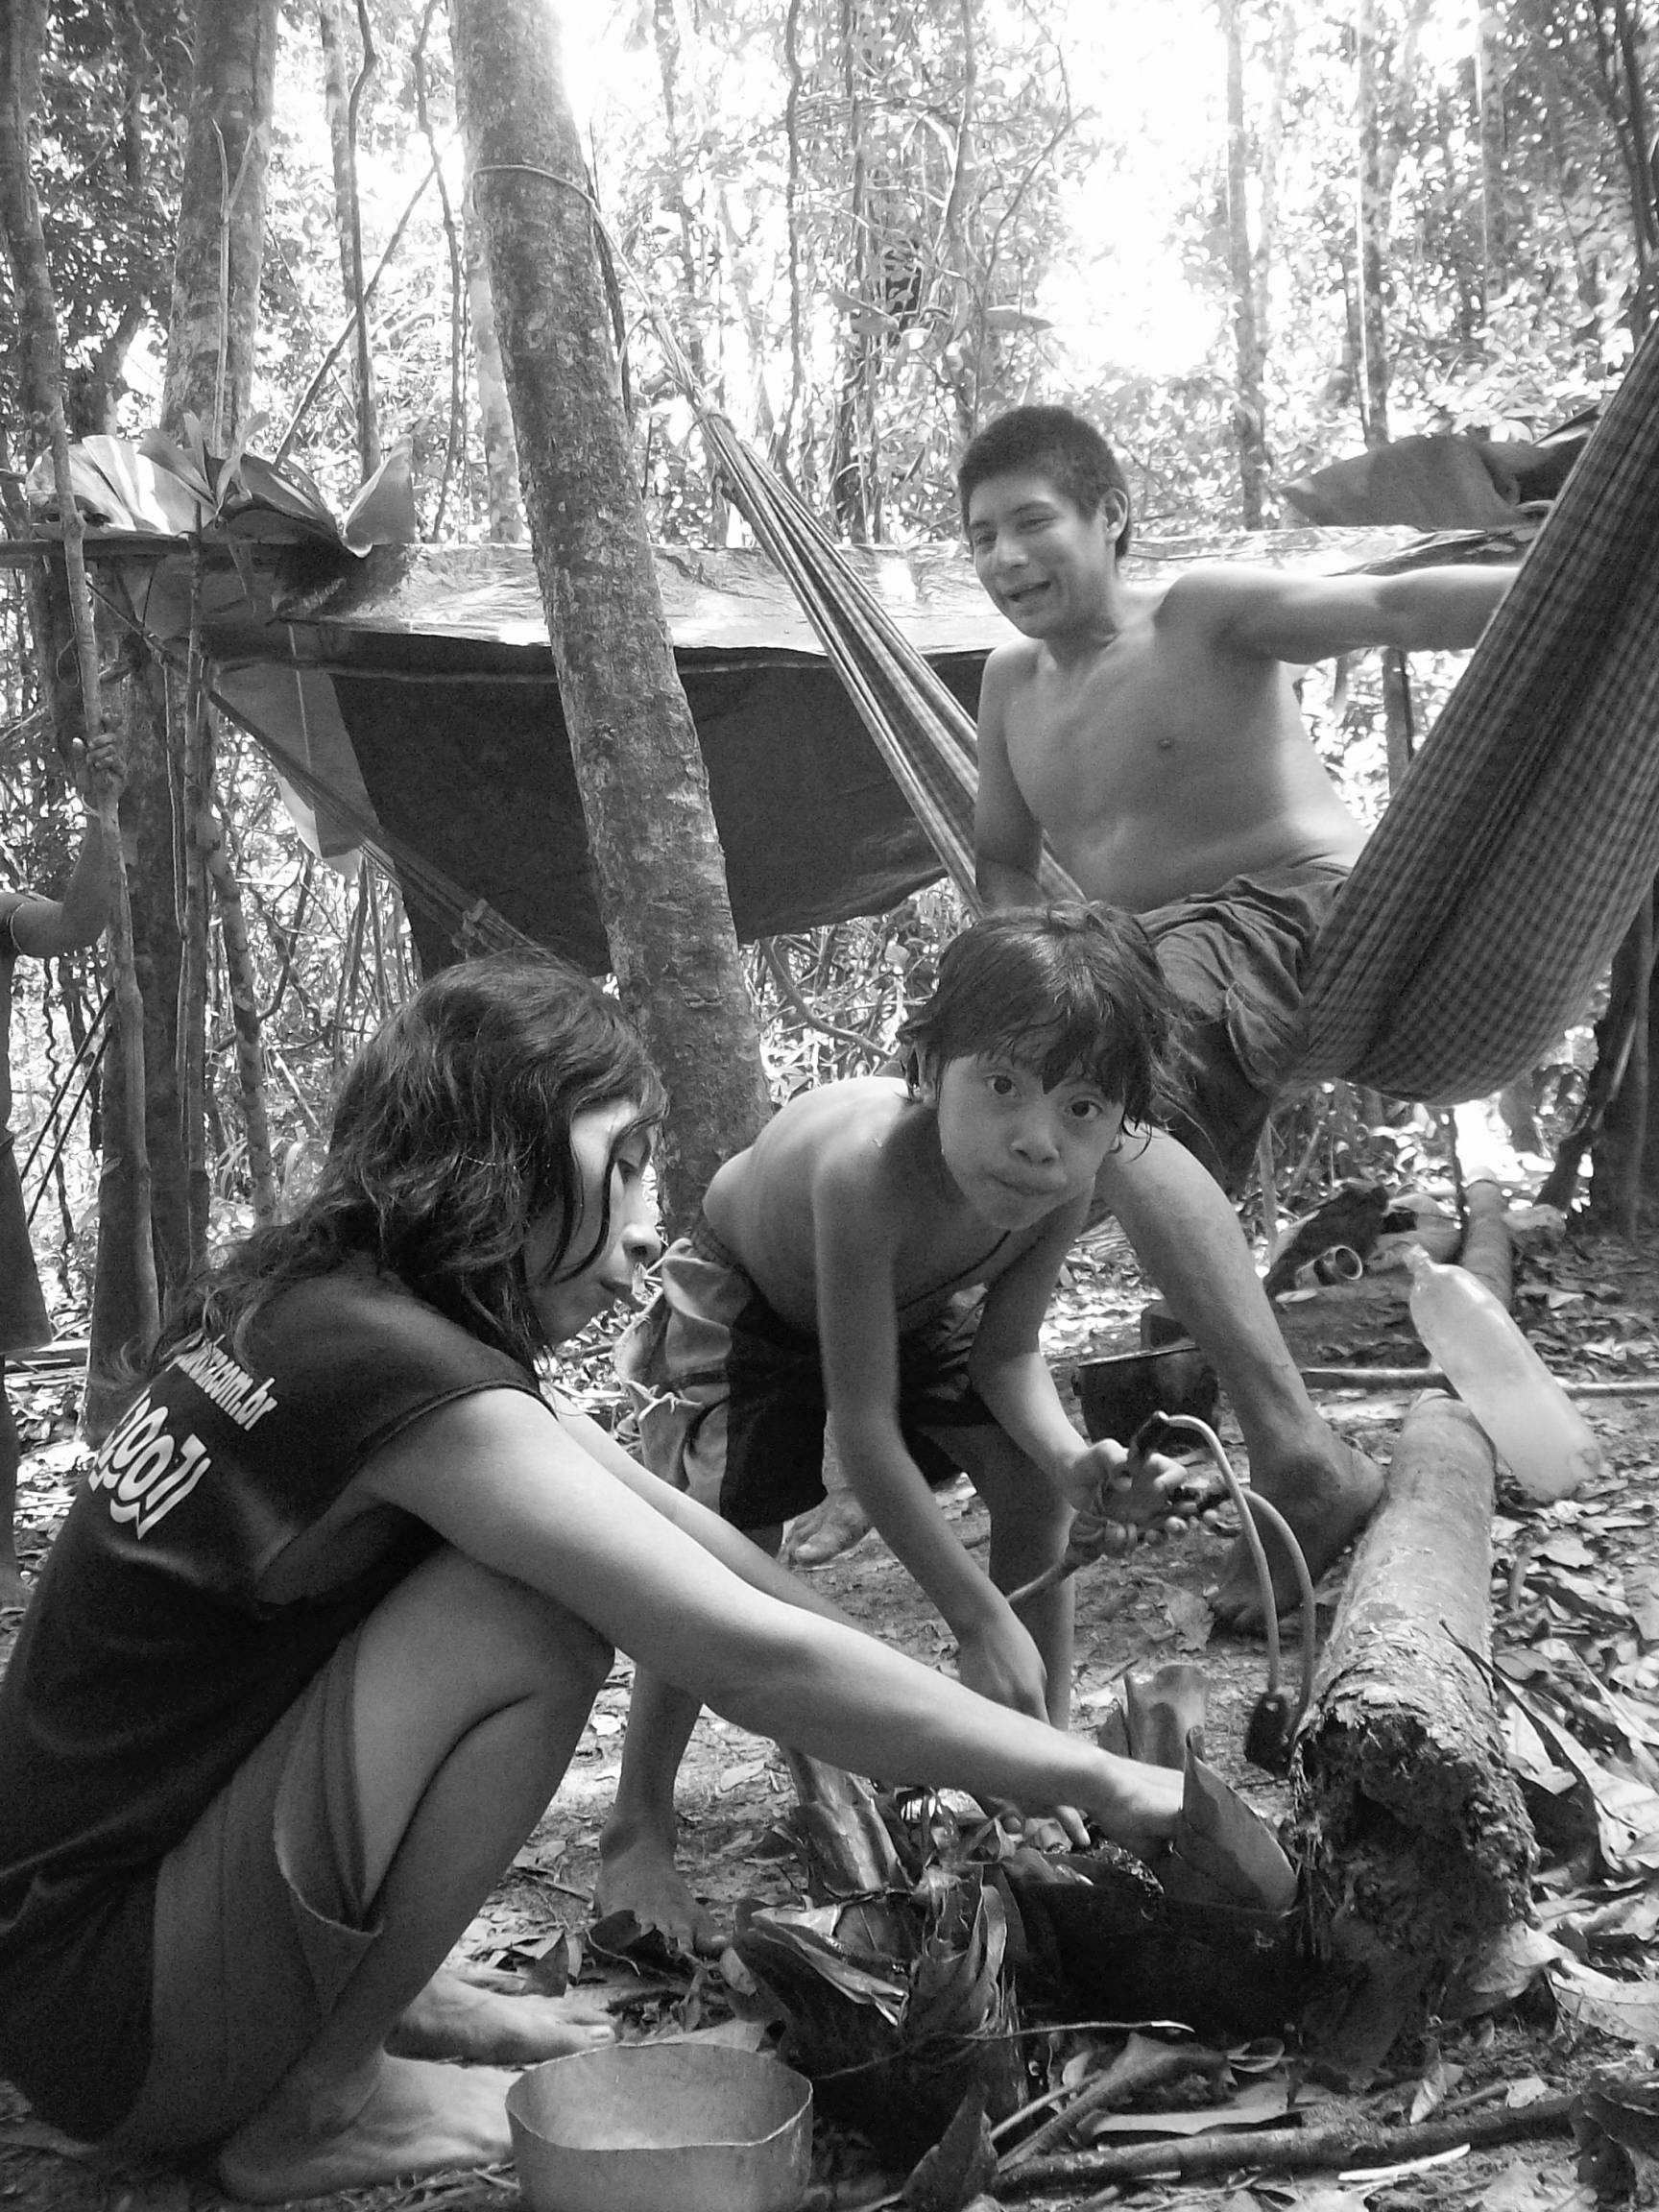
\includegraphics[width=85mm]{./imgs/100_4966}
%\caption{Ajrua, Uirahoa (sorrindo) e o pequeno Jahara em um acampamento de verão na floresta (aldeia Juriti, 2009).}
%\end{figure}

Ideias que definem os Tupi como notáveis agricultores --- beneficiadores
de diversas espécies de mandioca, lavradores aptos ao cultivo das mais
variadas culturas, da batata-doce ao fumo, passando pelo cará, milho,
amendoim, banana, pimenta, algodão, urucum, jenipapos e até cabaças;
produtores de farinhas e beijus; cauins fermentados e doces, dentre
outros cultivos específicos --- de forma alguma se aplicam aos
Guajá.\footnote{Para a relação entre os Tupi e a agricultura, ver os
  balanços de Laraia (1986) e Viveiros de Castro (1986).} A eles, como
vimos em sua história e, por consequência, no seu leque de opções
culturais, só restaram a caça de animais selvagens e a coleta dos frutos
da floresta. A agricultura está em uma fase embrionária, e o resultado
efetivo da incorporação dessa atividade no ciclo de vida das pessoas só
deverá ser percebido de forma qualificada dentro de algumas décadas com
o passar de, ao menos, mais uma geração. Enquanto isso, a caça, como
sugeri até aqui, segue como fenômeno central. Em nome dela, muitas vezes
estão dispostos a empreender um colossal investimento físico,
psicológico e mesmo emocional, e todas as outras atividades (pesca,
coleta de mel e frutos) parecem tributárias da caça. Muitos
acontecimentos se desenrolam a partir da caça: extrair mel, coletar
frutos (pequi, cupuaçu, bacuri, bacaba, inajá, dentre outros) e até
mesmo \textit{trabalhar} com a Funai são atividades passíveis de ser
abandonadas ou transformadas em caçadas, ao menor surgimento de um
rastro, indicação de um sonho ou mesmo pela pura \textit{vontade} de comer
determinada presa, como veremos mais adiante. O objetivo desse capítulo
é discutir os aspectos mais técnicos, psicológicos e econômicos das
atividades de caça e explorar o que seria, para os Guajá, essa atividade
--- como ela se inicia, o que é necessário para empreendê-la e outras
questões semelhantes.

Forline (1997), que realizou um estudo de alocação de tempo das várias
atividades desempenhadas pelos Guajá, demonstra como a caça é, dentre
todas as atividades, aquela com que os Guajá gastam mais tempo em seus
dias, mesmo não sendo a carne de caça a principal fonte de nutrientes.
Embora cacem com eficiência diversos animais, os Guajá são especialistas
na captura de mamíferos arborícolas, em particular cinco espécies de
primatas: o capelão (\textit{Alouatta belzebul}), macaco cairara
(\textit{Cebus kaapor}), macaco cuxiú (\textit{Chiropotes satanus}),
macaco-prego (\textit{Cebus apela}) e mão-de-ouro (\textit{Saimiri
sciuerus}). A técnica, que consiste em uma ``emboscada aérea'' dos
animais, ainda contemplaria a captura de quatis, ouriços-caixeiros, e
preguiças.\footnote{Tal como ocorre com outros animais que não são
  consumidos (ou são pouquissimamente consumidos), como a capivara e o
  tamanduá, as preguiças são abatidas sempre que os Guajá o conseguem.}
A pesca sempre foi tradicionalmente uma atividade residual, uma vez que
os Guajá sempre viveram longe dos cursos de grandes rios, não possuíam
canoa, tampouco uma técnica apurada para a captura de peixes. Tal como
os Parakanã ocidentais, cujas proteínas ingeridas até o contato eram
oriundas basicamente da caça, os Guajá também, durante o período
pré-contato, quando viviam na floresta, consumiam muito pouco peixe;
passaram a consumi-los com mais frequência após sua redução aos postos
da Funai (inclusive com o auxílio de linhas, anzóis e tarrafas
fornecidos pela administração do posto). Mesmo ``bater timbó'', como
fazem hoje, aprenderam com os integrantes das primeiras frentes de
atração. Embora os peixes não figurassem no topo das preferências
alimentares, os rios e igarapés abasteciam as pessoas com a carne de uma
espécie jacaré, \textit{jakarea}, e de poraquês, \textit{manakya}. Além
desses, alguns quelônios como tartarugas e capiningas (\textit{Trachemys
adiutrix}) são muito apreciados. Em geral, os peixes eram capturados com
timbó ou flechas no auge da estação seca.

Com essa breve introdução, pretendo apresentar neste e no próximo
capítulo o rendimento ontológico da caça no universo guajá. Mulheres que
caçam, flechas que ganham vida, xerimbabos que guiam os humanos no mato,
além das sortes e azares dessa atividade que, mais do que isso, é a
definição da própria vida para essas pessoas. Veremos como a caça Guajá
tem como resultado um profundo manejo de espécies silvestres, em que o
fato de não matarem os filhotes e os soltarem em sua idade jovem; o
respeito ao hábito das espécies, escolhendo apenas algumas horas para os
abater; e não destruírem árvores ``duras'' --- \textit{ira hatỹma'a}, ``madeira dura'' ---, 
lembrando-se de que são elas os verdadeiros
\textit{habitats} dos animais (em oposição às árvores finas e moles,
\textit{ira memeka}, ``madeira mole'') demonstram não só um profundo
conhecimento bioecológico, bem como constitui, de muitas maneiras, uma
manejo particular sobre o ambiente, como veremos.

\section{caçando com as mulheres}

Lembro-me, no ano de 2007, da primeira vez que fui convidado a
acompanhar um pequeno grupo em uma caçada simples, de um único dia. Por
ser uma caçada de pacas e cotias, saímos por volta das sete horas da
manhã (um pouco mais tarde do que se fosse uma caçada de macacos) e
voltamos um pouco antes do anoitecer. Era um grupo pequeno. Comigo,
contávamos cinco: um casal (Wirahoa e Ajruhua), Juxa'a (o filho mais
velho da mulher, com cerca de 16 anos) e o velho Takya. Ainda levamos
duas cadelas, fundamentais para rastrear pequenos animais. E Ajruhua
levou seu \textit{kwixua}, ``cuxiú'', de criação, empoleirado em sua cabeça e
que pulava de pessoa em pessoa, de galho em galho, e retornava às
cabeças à medida que caminhávamos.

Logo no início, percebi algo que seria recorrente a todas as caçadas que
eu iria presenciar: o fato de, se houver uma mulher adulta compondo o
grupo, toda a comunicação com os cães é feita por ela. Seus gritos
agudos são o sinal para que os cachorros, de longe, não parem de farejar
e respondam aonde estão. Os cães são delas! Durante todo o tempo, as
mulheres chamam pelos cães e eles, de longe, latem respondendo. E assim
segue, até que se ouve um latido mais forte, pontuado por rugidos,
acusando que encontraram a presa procurada. Nesse dia, após algumas
horas de caminhada, as cadelas rastrearam uma cotia que, poucos metros à
frente, se enfiara em um buraco. O terreno, muito acidentado, das serras
que compõem os territórios Guajá é formado por uma rede de buracos
feitos por tatus, pacas e cotias; muitos dos quais, ocultos, e que podem
ser chamados, como vimos, de \textit{akuti} \textit{rakwaha}, o ``domínio da
cotia'', --- buracos e troncos de árvores apodrecidos, os ``ocos de pau'',
que só um olhar especializado pode reconhecer. Ao encontrarem o
esconderijo em que a cotia se embrenhara, os homens começaram um
trabalho de escavação tão fundamental para a captura de cotias quanto de
pacas e tatus (durante o dia) --- para isso utilizam cavadeiras fornecidas
pela Funai. Em um período de quatro horas e em um raio de cinco metros
quadrados foram escavados sete buracos, alguns bem profundos.

Enquanto o jovem Juxa'a e o experiente Wirahoa escavavam as galerias
subterrâneas atrás do astuto roedor, quem indicava onde fazê-lo ---
ouvindo a movimentação da pequena presa, se alinhando de barriga ao chão
e enfiando a mão nas fendas aberta --- era a mulher, Ajruhua. A cotia não
se entregou facilmente: encurralada no final, após fugir pelo
subterrâneo e ser reencontrada através de um novo buraco escavado pelos
homens, o animal, mesmo sem saída, conseguiu se enfiar na terra de tal
forma que não havia braços ou varas longas o suficiente para alcançá-lo.
Nessa hora, Wirahoa junta alguns pedaços de palha seca de açaí, 
\textit{jahara}, pega em seu mocó o isqueiro com que o presenteei
semanas antes, ateia fogo nas palhas e, junto com Ajruhua, abana e
assopra a fumaça tóxica para dentro do buraco. Essa fumaça ``envenenará''
a cotia, ele explicou, e a deixará bem ``mole''. E foi isso o que
aconteceu. Minutos depois de o buraco estar repleto de fumaça, a mulher
conseguiu apanhar a cotia pelo pescoço --- que saiu se debatendo com muita
força. Uma vez fora do buraco, Ajruhua a domou, segurando as patas
inferiores com bastante firmeza, enquanto que, com a outra mão, apertava
a garganta até que o animal morresse por uma asfixia final. Enquanto
isso, seu marido e filho estavam calmamente conversando e se limpando;
cansados e aliviados.

Mataram a cotia sem disparar um tiro ou flecha sequer. E o animal morreu
pelas mãos de uma mulher: fato muito corriqueiro, como pude, depois,
constatar. Nessa ocasião, percebi (o que também é recorrente) que as
mulheres não estão ali como ``damas de companhia'', como se as caçadas
fossem algo exclusivo de um apartado universo masculino. As mulheres
Guajá problematizam a ideia de caçar como algo do universo masculino, ou
um fenômeno fortuito, caso os homens não estejam presentes, como na
descrição de Lima sobre a participação eventual das mulheres nas caçadas
de porcos dos Yudjá (1996, p.\,22). Ao contrário, aqui elas muitas vezes
não só propõem as caçadas, como podem andar na vanguarda de um grupo,
destacadas na frente, indicando para onde ir, comunicando-se com os
cachorros, rastreando fezes, urinas, pegadas, penas; enfim, todos os
tipos de vestígios, \textit{ipopora}, que devem ser sequenciados para que
haja uma caçada bem sucedida. Ajruhua é uma dessas mulheres. Seu marido,
Wirahoa, em 2007 era o melhor caçador da aldeia Juriti (em termos
absolutos, Wirahoa era o homem que trazia as maiores quantidades de
carne para casa). Porém quando caçam juntos, durante todo o tempo ele a
consulta sobre os caminhos a seguir e, muitas vezes, ela enxerga
possibilidades que ele não havia percebido. Como da vez em que ela
insistiu para andarmos um pouco mais, antes de desistirmos de uma vara
de porcos que, segundo muitos, já estava longe. E eis que encontramos os
porcos, após poucas horas de caminhada adiante. Enfim, ela tinha razão!

O fato de Ajruhua ser oito anos mais velha do que Wirahoa (ele tinha 29
anos em 2007, e ela, 36) pode ser um fator a se levar em conta; porém,
outros casais com idades próximas dividem com maior ou menor intensidade
o mesmo interesse pela caça: cada um de sua forma. Em uma tarefa
considerada universalmente masculina, a caça, inserida em um universo
como este --- em que predar é o centro da vida, e não uma atividade a mais
--- às mulheres só resta se juntar a seus irmãos, pais, maridos e
cunhados. Elas participam de todo o processo da caçada e podem,
inclusive, sair sozinhas a caçar (uma mãe e sua filha adulta, por
exemplo), principalmente cotias e pacas. Não é raro partirem de casa com
facões e machados e retornarem à aldeia com uma bela refeição e, ao
mesmo tempo, seus homens chegarem da mata, mas com as mãos vazias.

As mulheres desde muito jovens andam incansavelmente acompanhando também
seus namorados. Jovens namoradas, por serem alvo de muito ciúme da parte
de seus companheiros, não costumam ser deixadas sozinhas na aldeia
enquanto eles estão caçando. Elas, desde muito jovem, carregam seus
irmãos de colo ao acompanhar pais ou irmãos e, quando adultas, carregam
seus filhos junto com pesados machados, cavadeiras, facões e outros
instrumentos de metal. As mulheres ainda precisam dar conta dos
mosquitos e outros insetos, como mutucas e moscas, que, principalmente
na estação chuvosa, abusam da delicada pele dos bebês. Para afugentar
essas ameaças, cada uma delas porta um abanador, \textit{tata maka}, tal
como leques, que passam abanando sobre os filhos na tipoia durante toda
a caminhada. O leque, a tipoia, a saia, e o animal de criação, 
\textit{haima}, adornando a cabeça compõem a indumentária feminina
durante as longas caminhadas e caçadas.

Durante caçadas coletivas, ao encurralar algum animal, as mulheres podem
dispor de uma das flechas do marido. Elas as enfiam no buraco ou entre
as árvores, no intuito de ferir ou acuar a presa; se proteger ou ameaçar
algum animal; e não há restrições quanto a uma mulher tocar nos arcos ou
flechas de seus maridos. Muitas vezes, durante as caminhadas, se os
homens estão muito carregados, suas esposas levam para eles seus feixes
de flecha, arcos ou espingardas. Ao final de caçadas em que eu os
acompanhava, as mulheres gostavam de posar para minhas fotos segurando
os arcos e espingardas de seus maridos, bem como as caças abatidas por
eles. Quando posavam, diziam em tom de brincadeira terem sido elas que
mataram aqueles animais. E se cerca de uma década atrás as mulheres
seguravam arcos e espingardas apenas para aliviar o peso dos homens, nos
últimos anos, pelo menos em uma das aldeias, mãe e filha passaram a
caçar com espingarda. Ao visitar pela última vez a aldeia Tiracambu, em
2014, alguns amigos relataram o fato de Ximirapia e Pinawãxika, mãe e
filha, respectivamente, estarem caçando com uma espingarda que estava
``sobrando'' na casa de uma das duas, o que, definitivamente, me parece
uma novidade nesse estilo de caça realizado pelas mulheres. Estariam
elas matando inclusive macacos, algo até então nunca experimentado. Além
disso, os Guajá relatam que em situações excepcionais mulheres
confeccionam e utilizam arcos e flechas. Este é o caso das duas mulheres
encontradas ``isoladas'' em 2015 (a finada Jakarewãja e Amakaria), que
tiveram que criar sozinhas o pequeno Wirahoa. No mato, uma delas
fabricava arcos e flechas, caçava com eles e ensinou o menino a caçar
até que ele pudesse fazê-lo também.

É muito comum também as mulheres levarem às caçadas seus filhos com
idade de até dois anos. Levam-nos na tipoia, \textit{imymy menẽha}, que
até o contato era feita com fibras das folhas tucumã, mas hoje se faz
com tecido. Muitas vezes, devido às longas distâncias percorridas com as
crianças na tipoia, uma mulher pode pedir a seu marido que carregue a
tipoia com a criança por algumas horas. Nesse caso, ela mesma carregará
a espingarda ou arco e flechas do marido, em uma cena atípica na
literatura sobre caça, eu diria. Muitas foram as vezes em que os vi
trocarem os pesos ``masculinos'' e ``femininos'' para aliviar o desgaste da
mulher. Uma hipótese, que goza de longa história na antropologia, de que
as mulheres não caçam pois estão ``constrangidas, sobrecarregadas, ou
imobilizadas presas aos cuidados infantis'' (Noss \& Hewlett, 2001,
p.\,1025), tal como apontada por alguns autores (Brightman, 1996; Noss \&
Hewlett, 2001), também não se confirmaria aqui.

Não existem caçadas de que uma mulher não possa participar junto com seu
marido ou irmãos; é mesmo muito comum as meninas recém-noivas (ou
``pegas'', como dizem todos) e que ainda moram na casa dos pais
acompanharem os homens com quem irão se casar. Quase sempre, as
primeiras carícias e descobertas do sexo são experimentadas nesses
passeios de caça. Mesmo na caça de queixadas --- a mais desgastante e
arriscada dentre todas, pois os homens são obrigados a se separar, saem
completamente dos caminhos e trilhas usuais, se embrenham entre espinhos
e por áreas fechadas da mata (e tudo isso correndo\ldots{} correndo muito) ---
as mulheres podem estar presentes, embora, nessas situações, elas não
corram tanto nem se embrenhem com vigor entre espinhos e por áreas
fechadas, tal como fazem os homens. Caso estejam na mata em companhia de
seus maridos ou parentes do sexo masculino, as mulheres esperam em
algum local seguro; ou, se a caçada se estender por muitas horas,
simplesmente voltam à aldeia, sempre acompanhadas por algum homem
destacado para isso. Mesmo na caçada de porcos, em que dificilmente
elas participam diretamente da ação --- tal como fazem na captura de
outros animais ---, uma mulher pode ajudar seu grupo a rastrear os
queixadas e planejar estratégias de captura. Assim, de muitas maneiras
um casal pode ``andar junto'', \textit{wata} \textit{pyry}, atrás de caça; e o
interesse de uma mulher por caçar é considerado mais que desejável, uma
vez que, como estamos vendo, durante muito tempo essa foi a ``principal''
atividade na vida das pessoas.

Para os Guajá, portanto, nada mais ``natural'' do que mulheres se
envolverem nas caçadas. A partilha de interesse de uma mulher por essa
atividade, quase sempre, só tem a acrescentar ao desempenho de seus
maridos. Tenho, por suposição, que os melhores caçadores geralmente
contam com uma ou mais esposas interessadas no assunto. Ou, em outras
palavras, o sucesso na caça será consideravelmente superior para um
homem quando a mulher se envolve, uma vez que ela entende como poucos as
artimanhas dessa arte. Ajruhua e Amỹ Pirahỹa, por exemplo, quando saíam
com um grupo grande --- formado por filhos, maridos, irmãs e cunhados ---,
eram constantemente consultadas por homens para expressar suas opiniões
e decisões a respeito de determinados ``rastros'' (penas, fezes, urinas,
pegadas, tudo o que compõe a ideia de \textit{ipopora}, ``rastro'') e os
caminhos a seguir. O mesmo pude ver na aldeia Tiracambu, onde um dos
homens que mais capturava, Maihuxa'a, tinha em sua esposa, Pakawãja, uma
grande companheira de caça, muito interessada no assunto, e o casal, tal
como Ajruhua e Wirahoa, participava de todo o processo de caçada, que
consiste basicamente em rastrear, cercar e abater.

Uma ideia genérica de mulheres indígenas como coletoras de frutos ou
produtoras de beiju não expressa o forte comprometimento que as Guajá
mantêm com a atividade de caça. Além disso, muito do que é coletado o é
feito pelos homens, principalmente a bacaba e o inajá, frutos que são
apanhados por pessoas que têm que subir em suas árvores e que muitas
vezes têm como resultado cortes e escoriações profundas. Pequi, babaçu,
bacuri e cupuaçu realmente são possíveis de ser colhidos por mulheres e
crianças, porém, na época da bacaba (entre dezembro e março de anos
alternados), se não fossem os homens para apanhar os cachos, o consumo
da fruta não seria sequer metade do que é. Quero com isso defender que,
para os Guajá, a relação entre caça e coleta não está diretamente
condicionada aos sexos masculino e feminino, pelo que homens ``caçariam''
e mulheres ``coletariam'', tal como usualmente encontramos em textos sobre
grupos caçadores, passíveis porém de uma necessária crítica. Brightman,
por exemplo, argumenta que a generalização a respeito da ideia de
\textit{caça masculina} e \textit{coleta feminina}, tão difundida na
bibliografia etnológica a respeito de povos caçadores-coletores,
obscurece variações específicas do modo de produção particular
encontradas em cada sociedade em particular, já que em muitos contextos
as caças menores são capturadas por ambos os sexos ou, em alguns casos,
preferencialmente por mulheres (Brightman, 1996, p.\,689).\footnote{O
  trabalho em sociedades caçadoras e, mais especificamente, a
  contribuição das mulheres em caçadas é um tema bastante descrito na
  bibliografia acerca de povos caçadores-coletores. Ver Brightman (1996)
  ou Noss and Hewlett (2001).} Muito embora as mulheres não cacem como
homens --- uma vez que a diferença entre os sexos passa pela diferença
tecnológica: os homens utilizam armas; as mulheres, não ---, se aceitarmos
que as caças menores, junto com os capelães, representam a maior parte
da quantidade de proteínas consumida pelos Guajá,\footnote{Ver Forline, 1997.}
podemos apontar que as mulheres são componentes fundamentais a essa
atividade, e não meras substitutas ou colaboradoras. E mesmo o argumento
tecnológico --- tão definitivo para dar conta das assimetrias entre homens
e mulheres na caça, em que mulheres não usam armas, ``\textit{Ce n'est pas
la chasse qui est interdite aux femmes, ce sont les armes}'' (Não é a
caça que é interdita às mulheres, mas as armas), \footnote{Tabet \textit{apud} Brigthman,
\textit{op.\,cit.}, p.\,705.} se nos basearmos pelas ``mulheres caçadoras'' que
vivem em isolamento ou por Ximirapia e Pinawãxika, mãe e filha da aldeia
Tiracambu que vêm caçando com espingarda, tal afirmativa parece não se
aplicar totalmente no caso Guajá.

%\textbf{Mostrar foto de Pinawxiká com sua espingarda}
%\begin{figure}[H]
%\centering
%  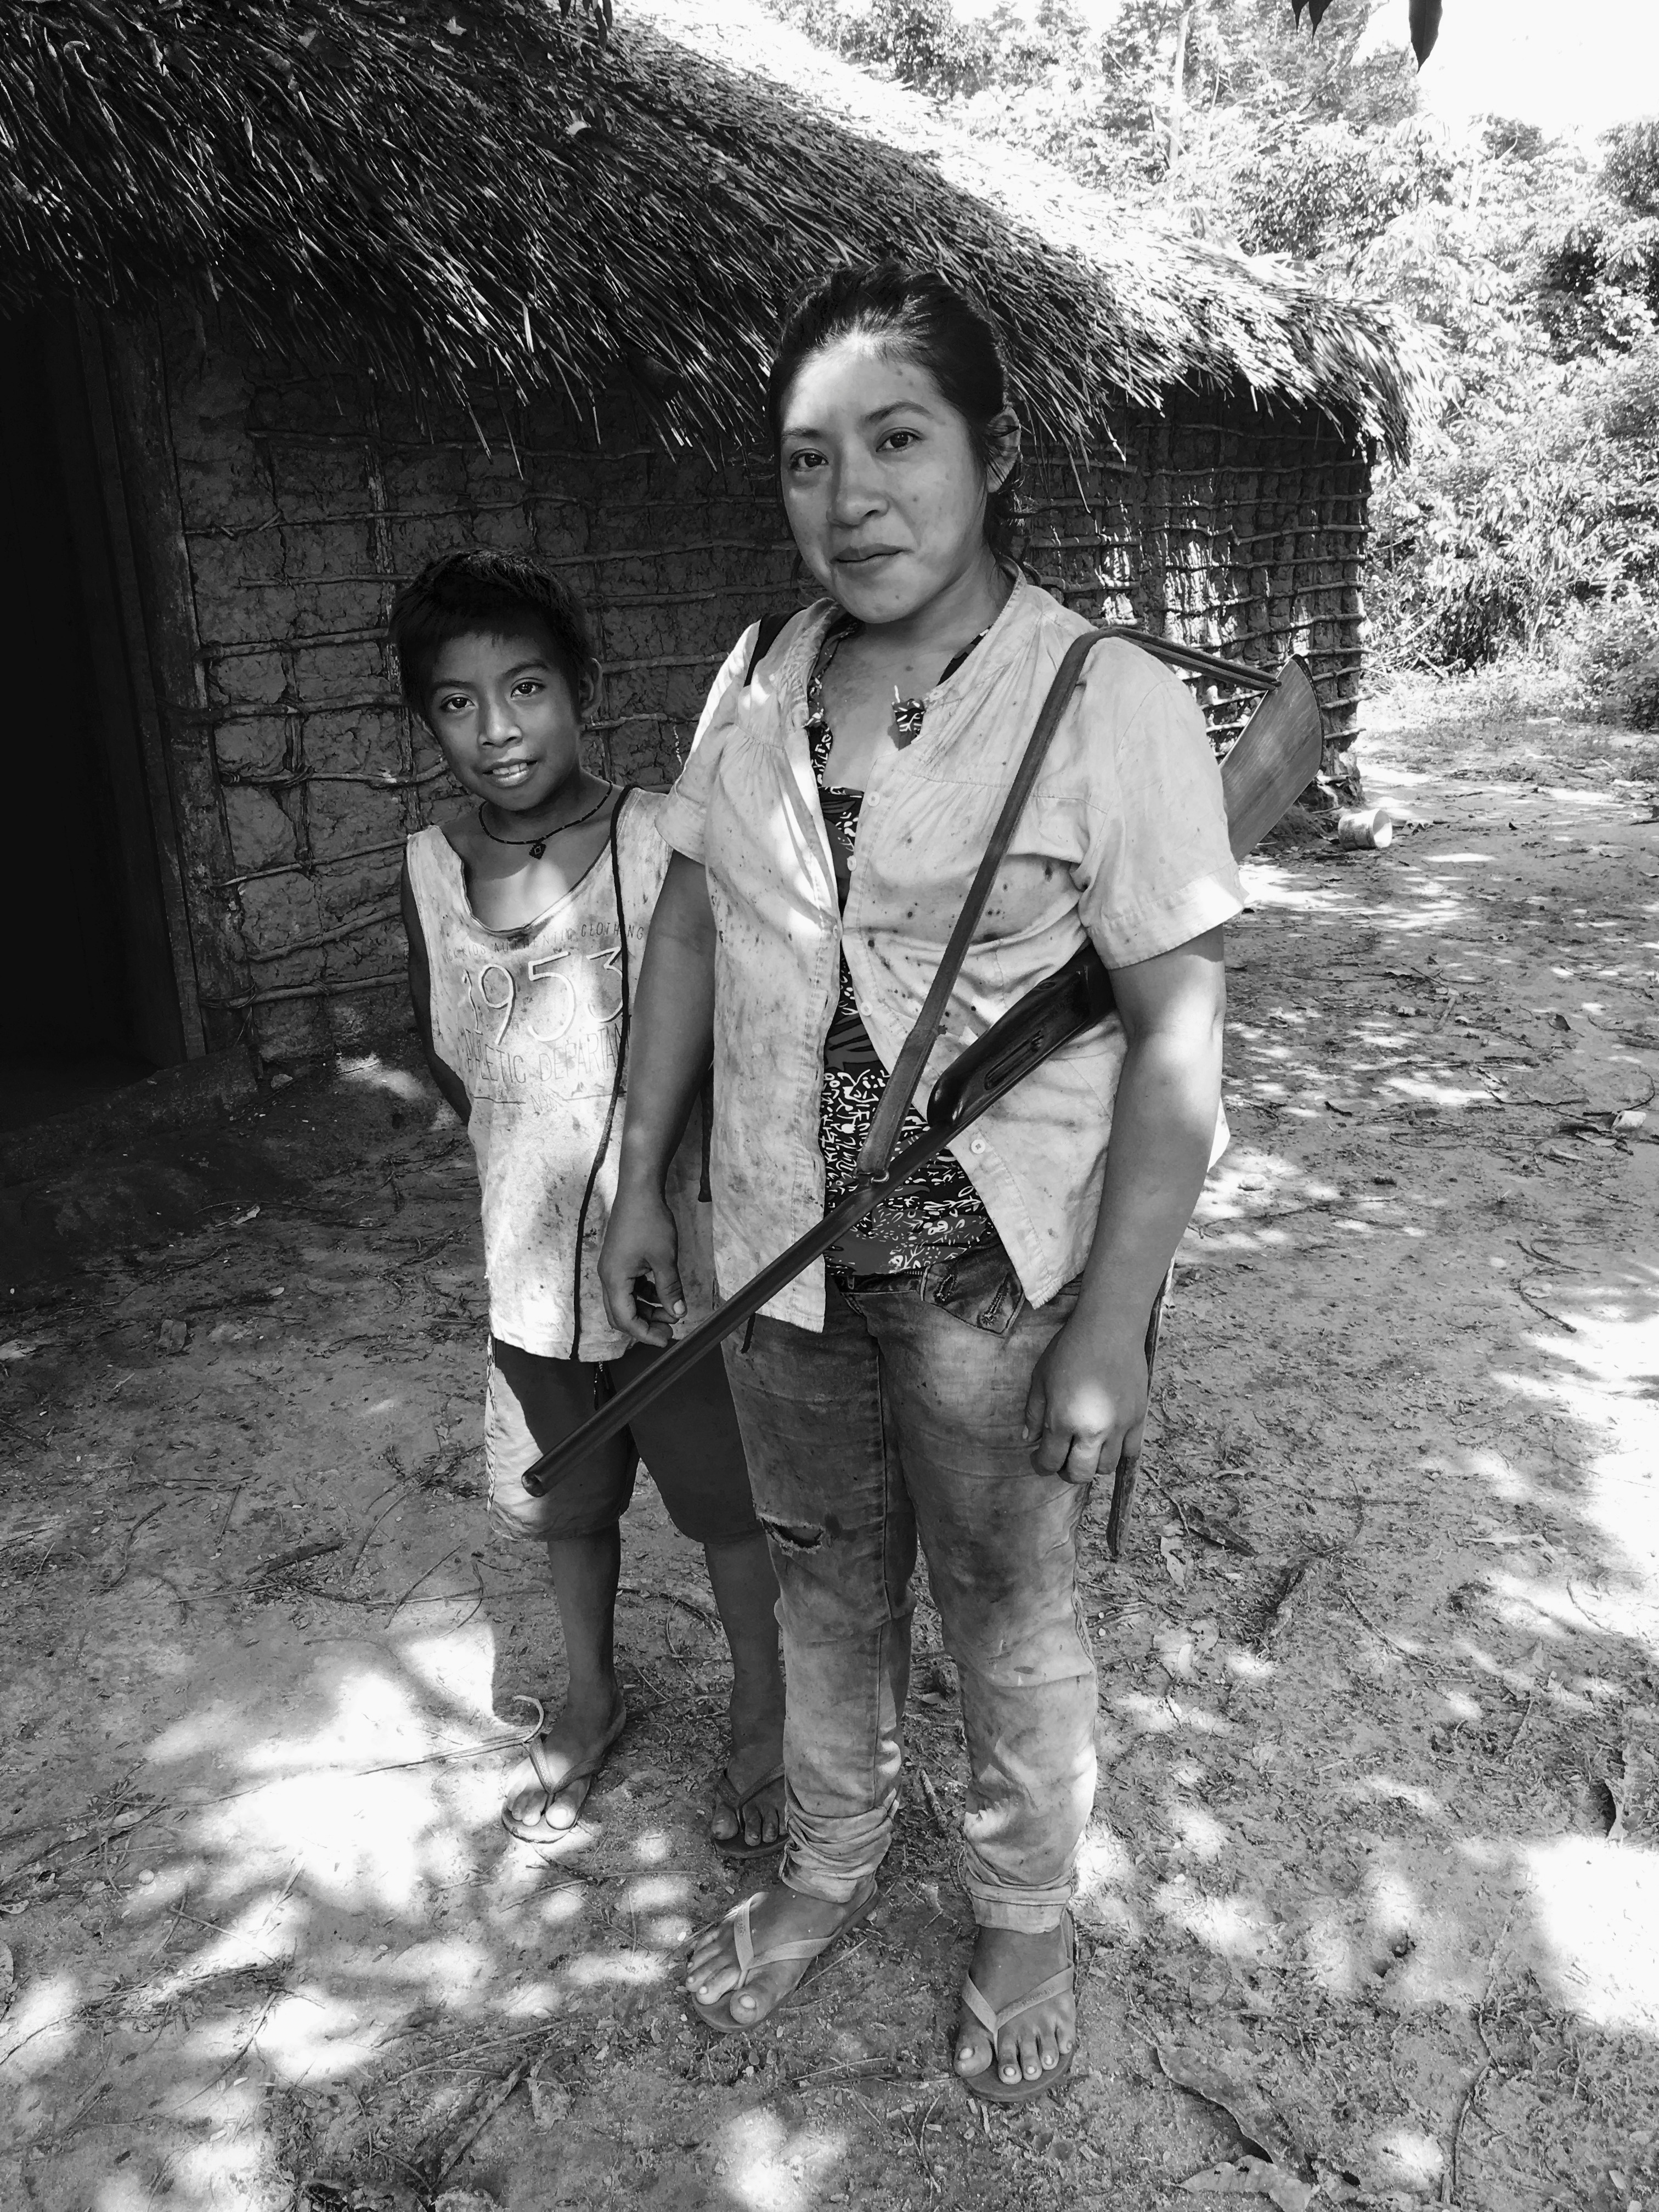
\includegraphics[width=\textwidth]{./imgs/IMG_4463}
%\caption{Pinawaxika, seu filho Ka'atatỹ e sua espingarda calibre 20, a caminho do mato (aldeia Tiracambu, 2018).}
%\end{figure}

Por outro lado, em nenhum momento os Guajá defendem a floresta como um
local seguro e prazeroso para uma mulher permanecer só, pois, mesmo
sendo caçadoras, são sensíveis à violência natural da mata. Apesar de
não excluírem as mulheres das caçadas (sendo, inclusive, desejável que
participem --- como estamos vendo) e muito embora defendam a presença de
suas esposas, irmãs e filhas nessa atividade, os homens guardam cautela
quanto à relação mulheres-mata. Mesmo sendo caçadoras --- \textit{watama'a},
``caminhador'' --- elas são desencorajadas por seus maridos em algumas
situações. São-lhes sempre lembrados os riscos de toparem com uma
onça-pintada (pois as sussuaranas e onças-pretas oferecem pouco perigo).

``Eu quero ver anta, veado, vamos andar-caçar, \textit{wata}, meu
marido!?'', assim Wirahoa sintetizou-me as chamadas de sua esposa para
irem caçar quase que diariamente. É uma atividade prazerosa para todos,
e as mulheres gostam, \textit{maparỹ}, da floresta como qualquer outro.
Porém, mesmo diante dos clamores exortativos femininos, os homens
guardam cautela à constante insistência delas para caçar, sejam
acompanhadas pelos homens ou por outras mulheres. A pronta resposta
masculina é, quase sempre, ``não vá, pois é perigoso, a onça te comerá!'',
ou outra coisa de ruim acontecerá. Em caso de encontro com as
onças-pintadas --- \textit{jawaruhua} ou \textit{jawarapeperemuhũa} ---, os homens
lembram que conseguem se defender e correr melhor do que as mulheres.
Além disso, Pakwa'ĩa, uma mulher, me explicou certa vez que as onças
preferem comer a carne feminina à masculina, bem como uma criança a um
adulto. Por essas e outras razões, uma mulher deve caçar de preferência
junto com o marido, \textit{wata} \textit{pyry}, embora isso não ocorra na
prática com a mesma frequência que é relatada no discurso dos homens.
Devo acrescentar que o ``fator cachorro'', como veremos neste capítulo, é
fundamental para que as mulheres tenham autonomia suficiente para entrar
sozinhas na mata; não só porque os cães espantam as onças e outro
animais perigosos --- proporcionando segurança ---, como também porque
facilitam, em muito, o trabalho de captura de roedores e tatus que, ao
lado dos quelônios, são animais facilmente capturados e abatidos por
mulheres.

O fato de a floresta ser supostamente mais perigosa para uma mulher que
para um homem parece ser, ao menos aparentemente, algo com que todos
concordam; pois os homens, pelo fato de possuir armas, conseguir subir
em árvores, aguentar mais peso, dentre outras vantagens técnicas,
seriam, pelo menos dizem os Guajá, mais preparados para enfrentar a
mata. É interessante notar que, apesar da ideia de ser a floresta um
local perigoso para as mulheres --- e do fato de os homens em geral se
utilizarem de armas, e as mulheres não ---, em nenhum momento homens
defendem que a caça é uma atividade \textit{masculina} em oposição a outra
atividade (como a coleta) que seria \textit{feminina}. Evocando aqui a
crítica de Marilyn Strathern (1980), o próprio par referente à
\textit{esfera doméstica}, representada pelos animais de criação ---
filhotes cujo manejo da vida depende das mulheres ---, e a \textit{esfera
selvagem} concebida quanto a animais de caça, em que os homens são
agentes privilegiados dessa relação, deve ser visto com cautela, uma vez
que os animais de criação que acompanham mulheres à mata ali estão não
apenas como adereços para o corpo (como já tentaram sugerir). Em conexão
com suas donas, macacos pregos e cairara, atentos às caminhadas, podem
alertar com assobios e gritos sobre cobras e aranhas venenosas durante o
trajeto (Diniz, 2014, p.\,65). O mesmo pode ser visto --- como observaremos
mais à frente --- com os cachorros. Desde a introdução desses animais nas
atividades de caça, as mulheres passaram a andar com mais segurança no
mato, com menos ameaça de serem atacadas por onça, e grupos de mulheres
com seus cachorros costumam ser muito eficientes em caçadas. Se a
floresta é um local perigoso para as mulheres, como os homens costumavam
me dizer, com os cães os riscos são amenizados. Os animais de criação
aqui, longe de serem exclusivos da aldeia --- \textit{esfera doméstica} --- em
oposição à pura predação de uma suposta \textit{esfera selvagem}, são
importantes justamente na mata.

Sabemos há algum tempo que as diferenças entre mulheres e homens não
estão necessariamente baseadas na divisão entre natureza e cultura,
muito menos podem ser diretamente correlacionadas a uma oposição entre
\textit{doméstico} e \textit{selvagem} (Strathern, 1980). Como já pontuado aqui, a
questão de homens desaconselharem mulheres a entrar sozinhas na floresta
e o fato de a caça acontecer na mata não podem ser reduzidos à ideia de
que a caça seja uma atividade masculina por excelência, embora seja
bastante desejável pelo mulherio, \textit{awa wahykera}, que os homens
cacem para as esposas, e muito do que as mais velhas almejam ao se casar
com homens mais jovens é que eles caçarão para elas. Porém, nem por isso
a caça é pensada como uma atividade exclusivamente masculina.

Para os Guajá, o selvagem, \textit{ka'a}, e o doméstico, \textit{tipa}, não
parecem encontrar ecos automáticos em outras oposições (supostamente)
manifestadas como masculino e feminino; humanidade e animalidade. Por
isso, o problema aqui, mais uma vez, repousa na imposição de uma
dicotomia analítica a situações em que ela não é apropriada (Strathern,
1988, p.\,20). A ``animalidade'' de um animal de criação, muito
provavelmente, em nada se conecta à animalidade de um animal selvagem
que será caçado. Diferentes modos de relação recortam os animais em duas
categorias distintas entre si: \textit{hanima}, ``meu animal de criação'',
e \textit{ma'amijara} ou apenas \textit{ma'a}, ``presa'', ``caça'',
``bicho''. Um animal que é tratado por presa nunca será de criação, e
os filhotes capturados dessas presas (apenas os muito pequenos)
raramente são vistos como ``caças'', \textit{ma'amijara}. Os filhotes
capturados devem ser muito pequenos, pois aqueles um pouco maiores são
difíceis de amansar e ainda poderão, em algum momento, se vingar da
morte de seus pais, atacando principalmente as crianças. Filhotes de
macacos, queixadas, caititus, esquilos quatipuru, cotias, papagaios,
quatis e macacos-da-noite são criados na aldeia, e quase todos
acompanham suas donas em caçadas e incursões pela floresta. O fato de
animais serem domesticados é o que, de muitas maneiras, colabora para
que as mulheres cacem mais, com mais vigor e qualidade, e mais ainda as
remete --- com mais segurança, pois esse é um ponto importante aqui --- para
a floresta.

\section{a vontade de \textit{querer ver}}

Em sua teoria sobre a caça, os Guajá defendem que a vontade de matar um
animal específico é fundamental a uma caçada produtiva. Certa vez, após
passar um dia na floresta acompanhando Pira'ima'ã, voltamos para casa
com as mãos vazias, reflexo do péssimo dia de caçada. Em nossa caminhada
de retorno, Pira'ima'ã comentou: \textit{axaku'uhy wari ikaha}!, sentença
que pode ser traduzida por algo como ``estou com muita vontade de matar
capelães!'' Isto indicava que o fato de não os ter matado poderia,
inclusive, lhe fazer mal, já que aumentava cada dia mais essa vontade,
que é chamada \textit{xaku'uhy} e permite uma tradução como ``querer ver''.

De acordo com Magalhães,\footnote{Comunicação pessoal.} \textit{xaku'uhy} é um verbo que
pode ser traduzido grosseiramente por ``sentir falta'' ou ``ter saudade''.
Mas, analiticamente, ele pode ser segmentado em três partes: \textit{xak}
``ver''; \textit{u'u}, um morfema encontrado em poucas palavras e que
significa ``desejar'', ``querer''; e \textit{hy} um sufixo que indica a maior
intensidade com que é empregada a palavra.\footnote{\textit{I'ĩ}
significa ``ele falou'' e \textit{i'ĩ-hy}, ``ele ralhou'' ou ``falou de maneira
mais forte''.} Dessa forma, ``ver'', \textit{xak}, ``querer'', \textit{u'u}'', isto
é, ``querer ver'', parece uma tradução satisfatória. No caso em questão,
Pira'ima'ã estava com vontade, ou ``saudade'', de comer capelães. Isso
pode ser bom, pois promove novas caçadas; mas também pode ser ruim, pois
a frustração acarreta problemas.

Por exemplo, em uma caçada há sempre uma predisposição para matar
animais movida por uma vontade que não será saudável se for frustrada.
Caso seja frustrada, deve ser sanada. Tal vontade pode ser produzida por
algum evento: como um sonho, uma conversa, o conhecimento de um novo
rastro e mesmo, obviamente, a fome.\footnote{\textit{Hajamyhỹ}, ``estou com
fome''.} As duas ou três refeições que os Guajá gostam de fazer em um
dia são completadas por ceias menores, compostas por frutos, pedaços de
carne, mel com farinha, hidromel, iguarias como fígados, língua e
cérebro de alguns animais, bolachas e toda sorte de alimentos que
estiverem ao alcance da mão. As crianças são capazes de passar os dias
comendo, e são justamente elas e as mulheres que mais exigem comida. Em
um belo relato sobre os Aikewara, Tupis do leste do Pará, Calheiros
afirma que ``um caçador, se for perguntado sobre os motivos que o levam
a abandonar a sua rede e partir para a mata em busca de caças,
responderá indicando uma mulher que vive junto dele: os solteiros dirão
que caçam para suas mães e irmãs mais novas, os casados, que caçam para
suas mulheres e filhas'' (2014, p.\,177); e essa ``fome'', destaca
Calheiros, mobiliza as comunidades e mantém os homens em movimento. Nas
aldeias Guajá, crianças famintas ficam muito zangadas e, por isso, podem
brigar entre si, chorar de forma desmedida, bater em xerimbabos e, mais
comum do que possa parecer, arrancar os próprios cabelos em desespero.
Os pais sempre que saíam para caçar diziam a mim, mesmo em português,
``tenho que caçar, as crianças estão com fome!'' Por isso, a
``vontade'', para ser aplacada, quase sempre nem será a própria vontade
do caçador, mas a dele e a dos outros relacionados a si (mulheres,
filhos), o seu \textit{pessoal}, para evocar a tradução dos Yudjá (Lima,
2005, p.\,110).

Uma caçada frustrada, perdida, ou não realizada, pode criar um desejo de
matar ainda maior, deixando os homens transtornados, \textit{waky},
com raiva, \textit{imahy}, acumulada, o que os obriga a ir para
a floresta muitas vezes sozinhos e só voltarem quando a raiva tiver
passado --- o que só acontecerá após matarem o máximo de animais que
conseguirem. Por outro lado, essa vontade, \textit{xaku'uhy}, ``querer ver'',
é umas das características que mobiliza os Guajá para a caça. A relação
entre vontade e ação não tem um centro fixo de irradiação. Não há uma
palavra de ordem que os mobilize para a caça ou qualquer outra
atividade. E os eventos podem ocorrer como que por ``vontade própria''.

Certa vez, após comermos muitos inajás, fiquei curioso para experimentar
o coco desse fruto, pois, como se sabe, do inajá consumimos somente o
fruto --- cozido, assado ou na forma de mingau --- e seu coco é normalmente
descartado. Alguns me disseram que não comiam o coco do inajá pois a
casca, além de muito dura e difícil de arrancar, escondia um coco muito
pequeno, cujo esforço não valeria a pena. Nessa manhã, talvez por falta
do que fazer, peguei emprestada a cabeça de um machado e um toco de pau
a fim de abrir alguns cocos de inajá que abarrotavam o chão, em volta de
um moquém, onde haviam sido cozidos. Ajudado por alguns meninos, comecei
a atividade. Assim que abri o primeiro coco, logo me decepcionei,
constatando que era preciso um esforço muito grande para retirar a casca
e que o resultado era uma noz pequena e sem gosto, quando as pessoas me
disseram em tom de galhofa: \textit{kwaj kĩ mehẽ!}, ``tá vendo!?'' ou ``não
disse!?''. De todo modo, prossegui na operação, abrindo mais cocos ---
mais por esporte do que por outra razão. Logo vi que estava sendo
acompanhado por alguns garotos que faziam o mesmo. Minutos depois, boa
parte das crianças da aldeia estava espalhada quebrando cocos de inajá
para comer. Em seguida apareceu Pira'ima'ã, querendo amolar meu machado.
E passou, ele mesmo, a quebrar cocos de inajá; chegou também sua mulher,
Pakwa'ĩa, e instantes depois, seu pai, o velho Pirama'ã, além de outras
pessoas. Em menos de meia hora, um exercício inútil movido por uma tola
curiosidade havia se transformado em uma ocupação que tomou dezenas de
pessoas da aldeia Juriti. Da mesma maneira, muitas vezes os desejos,
inclusive por uma caçada, podem se iniciar desta forma, meio que por
contágio.

Por isso, há uma grande dificuldade por parte dos funcionários da Funai
de arregimentá-los para os trabalhos da roça, pois palavras de mando não
surtem o mesmo efeito que uma epidemia de vontades. É comum os
funcionários marcarem uma colheita ou plantio para o dia seguinte e, na
hora em que estão indo para a roça alguém anunciar um novo rastro de
porcos ou um grupo de capelães; e então, todos abandonarem o \textit{trabalho},
deixando os funcionários sozinhos na roça. Em outras diversas situações,
quando um trabalho na roça ou no pomar não estava marcado, as pessoas
muitas vezes se encaminhavam uma a uma (tal como no episódio do inajá)
para trabalhar, deixando os funcionários do posto sem entender, já que
isso não estava previamente ``combinado'', isto é, não tinha havido
palavras de mando. Simplesmente os Guajá começaram. Não se trata somente
de a roça ser algo menos interessante do que a caça (o que é fato), mas
a forma como se inicia uma atividade nem sempre é escolhida por todos.
Simplesmente começam, como se fossem tomados por uma grande vontade
mobilizadora, que defendo aqui ser o \textit{xaku'uhy}, ``querer ver'',
importante tanto para a caça quanto para a vida, de maneira geral.

Viveiros de Castro, como lembrou Fausto, \textit{descreveu com elegância o
caráter epidêmico das ações coletivas em uma sociedade sem chefia}
(Fausto, \textit{op.\,cit.}, p.\,275):

\begin{quote}
Fruto menos de deliberações formais ou tomada de decisão de alguns em
nomes dos outros, os atos concertam-se por um processo social de
contágio. Ninguém diz a outrem o que deve fazer, mas sugere o que ele
próprio fará. {[}\ldots{}{]} é preciso, contudo, que alguém dê início à ação,
tirando da inércia as disposições.
\end{quote}

Fausto comenta como tal característica se presta à guerra Parakanã
(Fausto, \textit{op.\,cit}., p.\,275), e Viveiros de Castro, como tal \textit{caráter
desordenado e paulatino}, rege boa parte das ações dos Araweté (Viveiros de
Castro, 1986, p.\,300). A partir de noções específicas sobre as relações
humanas, tal como \textit{tenetãmõ}, ``o que segue à frente'', e
\textit{tãnã}, ``o dono da aldeia'', Viveiros de Castro observa que ``toda e
qualquer empresa coletiva Araweté supõe um \textit{tenetãmõ}'', e ``uma
coisa não começa se não houver alguém em particular que a comece''.\footnote{\textit{Iidem}.}
O cognato Parakanã para o \textit{tenetãmõ} dos Araweté é
\textit{tenotara}; na guerra, eram eles que iam à frente, eram os
primeiros, dotados de uma grande capacidade exortativa (Fausto, \textit{op.
cit.}, p.\,276). A ideia de \textit{tãnã} Araweté, que está baseada na
aldeia, no componente espacial, encontra entre os Guajá o termo
\textit{tamỹa}. Por isso, aludem para o fato de \textit{Maira} ser um
\textit{iwa} \textit{tamỹa,} um líder nas aldeias celeste.

Se o problema da liderança, mais do que chefia, como parece ser, é este
de fazer aparecer um coletivo em que o líder é aquele que inicia,
coordena ou mesmo captura uma ação (Sztutman, 2012, p.\,316), os Guajá
lembram que o \textit{chefe} (sendo esta uma glosa indígena) é aquele que
``puxa'' uma ação coletiva. Uma ideia importante na política é aquilo
que traduzem para o português por ``puxar''. \textit{Myty}, ``puxar'',
seria a principal atribuição de um \textit{tamỹa}, o \textit{chefe}; que vai
na frente). \textit{Myty ipamẽ} pode ser traduzido por ``puxando juntos um
ao outro'', e os trabalhos na roça, caçadas e outros movimentos são
sempre assim concebidos. Para todas as atividades, além de outros níveis
da própria existência, as figuras de \textit{tamỹa} ou \textit{xipa}
\textit{tamỹa}, o ``velho'' ou ``pai que lidera'', são sempre evocadas. E apesar
da complexa e, muitas vezes, categórica diferença entre ``chefia'' e
``liderança'', tão bem documentada em trabalhos como o de Sztutman
(2012), a glosa guajá para essa figura do líder --- o que toma a frente e
mobiliza um coletivo --- é sempre \textit{chefe}, e mais recentemente
\textit{cacique}, como é o caso de jovens chefes de família que acumulam
uma função no diálogo interétnico contemporâneo que, como bem mostrou
Yokoi (2014) em sua dissertação sobre política Guajá, ainda estamos
vendo para onde levará a se mover a figura do \textit{cacique}. Quando
todos os chefes de família se pensam e são pensados como \textit{tamỹa},
em situações de tradução como nas reuniões com a Funai ou \textsc{sesai}, muitas
vezes os jovens \textit{caciques} dizem que não conseguem despertar o
interesse de toda uma aldeia para uma atividade previamente acordada com
o órgão; quando muito, eles o conseguem com suas famílias e aliados.
Certa vez, o jovem Manã, da aldeia Awá, explicitou tal problema
em uma conversa de ``líderes'' --- leia-se jovens interlocutores --- com a
equipe de índios isolados da Funai, lembrando que tudo aquilo que eles
estavam combinando ali (mudança no jeito de fazer as roças, usos das
torneiras da aldeia dentre outras importantes decisões) de nada
adiantaria, pois quando ele voltasse para casa o combinado funcionaria
melhor para seu grupo de parentes e amigos do que para os outros. A
profusão das figuras de \textit{chefia} nas aldeias maiores também é
discutida por Yokoi, aludindo à conhecida diversidade de grupos locais
nos diversos territórios, \textit{hakwaha}, antes do contato. Com isso,
\textit{tãmya}, segundo o autor, ``poderia ser considerado como o dono do
espaço de circulação de seu grupo, tendo em vista a mobilidade Guajá em
seus \textit{hakwaha}. {[}\ldots{}{]} Como a aldeia Awá é uma reunião de vários
grupos dispersos podemos encontrar muitos \textit{tãmy} por lá, diria que,
\textit{tãmy}, são todos os homens com mais de trinta anos e que de certa
maneira são ativos na vida pública da aldeia'' (2014, p.\,144). Ainda há
uma relação direta entre chefia e xamanismo pois, como veremos no último
capítulo, a figura do cantador, rezador e curador, encarnada pelo xamã,
é ocupada também por todos os chefes de família e homens adultos quase
que de forma geral. E nas palavras de Yokoi ``{[}\ldots{}{]} \textit{tãmy} é ser
xamã, é permitir e fazer com que o sopro e o canto dos \textit{karawara}
continuem dando a vivacidade e a alegria para que a abundância celeste
seja presentificada aqui na Terra'' (Yokoi, 2014, p.\,146).

Devo lembrar que ao chegarmos a uma aldeia guajá os primeiros termos
vocativos que ouviremos provavelmente serão \textit{xipa} e \textit{amỹ},
``pai'' e ``mãe'', respectivamente, mas que ganham um espectro de
aplicação bastante amplo. Ambos são termos que podem ser aplicados para
homens e mulheres de uma ou mais geração acima e mesmo --- na fala --- entre
cônjuges e irmãos, como já discutido aqui. Depois destes, \textit{xipa}
\textit{tamỹa} aparece como um termo de referência muito recorrente. Todo chefe de família que já tenha tido um neto; pessoas não indígenas com cabelos grisalhos; e todos os homens que evoquem uma idade um pouco mais avançada ou mesmo a proeminência (devido a sua idade) sobre outros homens são chamados de \textit{xipa} \textit{tamỹa}. Esse último termo,
portanto, encarna diversos papéis, como xamã, ancião, dono de atividade,
dono de área de caça, \textit{hakwaha}. Depois do fim das aldeias
dispersas e a retomada da vida em grandes aldeias únicas, o que
observamos são comunidades com muitos ``chefes de aldeia'', cada um
preocupado com sua sessão, sua área de caça e roça.

Parte do movimento é desencadeada pela vontade desses homens, muitas
vezes, como se espera, um sogro, pai ou cunhado importante, e tal
vontade, \textit{xaku'uhy}, quase uma clarividência, é central em todo
esse processo. Essa versão guajá do \textit{tenetãmõ} Araweté,
\textit{tenotara} Parakanã, ou mesmo do \textit{iju'a} Yudjá\footnote{Trata-se de uma ação
que permite o movimento de um coletivo, além de se dar de maneira
contagiosa; propulsada por tal figura, porém sem palavras de mando;
motivada por causas diversas, naturais ou extra-naturais.} é de fato
próxima desses outros Tupi (Sztutman, 2012). E no mundo guajá e na caça,
mais especificamente, essa forte vontade, \textit{xaku'uhy} ``querer ver'',
se coaduna a esses estopins iniciais que mobilizam um caçador e seus
aliados para caçar. A vontade \textit{xaku'uhy} é o motor da caça e
produz, inclusive, uma raiva\footnote{\textit{Imahy}, `` estar com raiva''.} que, se
bem canalizada, será uma grande aliada durante as caçadas.

Caçadores mais experientes, mais velhos, conseguem controlar e canalizar
essa vontade de matar, \textit{xaku'uhy}, de uma maneira mais eficiente
que os jovens. Esses últimos são literalmente tomados pela raiva quando
estão vivendo seus anos iniciais como caçadores. E enquanto alguns
conseguem se controlar outros sucumbem a uma total falta de controle.
Por exemplo, um jovem, que em 2009 estava com 14 anos, havia abatido
dois dos seis capelães que seu grupo (formado por seu pai, tio {[}\textsc{fb}{]}
e outros aliados) matara, e voltou para aldeia ainda muito excitado pelo
feito. Terminada a caçada, ao retornar para casa --- gritando e empunhando
seu arco --- começou a perseguir um galo que estava próximo. Por fim,
conseguiu flechar a ave em um dos olhos para, na sequência, atirar
flechas em panelas, cuias e outros objetos que encontrava pelo caminho.
Não satisfeito, voltou a procurar galinhas para matar, até que sua mãe,
muito calmamente, o aconselhou a ir tomar um banho no rio. Perguntei
para seu pai o que estava acontecendo, e ele me disse, em português, ser
``assim mesmo''; ``o menino está com vontade de matar!'' Os homens adultos,
mais experientes, ao contrário, são extremamente silenciosos durante e
após uma caçada. Mesmo em caçadas gregárias, como a de capelães, podemos
ouvir mulheres e crianças gritando muito em momentos de correria e
abate, já os homens nada falam. Muito silenciosos, dizem que ``os animais
ouvem'', \textit{nũ}, sobretudo as vozes dos caçadores, por isso não devem
pronunciar muitas palavras nem ficar nervosos. Quando acabam uma caçada
e voltam para casa, deixam a caça cair no chão, e normalmente se referem
à esposa com frases do tipo: \textit{kararuhu ajka harimirikoa}, ``minha
mulher, eu matei paca'', ou \textit{wari ajka harimirikoa}, ``minha
mulher, eu matei capelão''. Não se trata de uma fala cerimônial, mas um
``jeito'' de falar --- \textit{a'e kĩa}, ``é assim mesmo'' --- na volta das
caçadas. Depois disso falam baixo e descansam muito. Só rompem o
silêncio para narrar como foi o dia na mata, a captura dos animais ou
indicar para quem pretendem dar um pedaço da carne. Por outro lado,
muitos dos jovens que começam a caçar (porém nem todos) por volta dos 13
anos (e algumas vezes bem antes)\footnote{Entre os Guajá, um menino com
  nove ou 10 anos de idade já é capaz de capturar pequenos mamíferos,
  como cotias e tatus; pássaros que servem para a alimentação, como o
  juriti-gemedeira (\textit{Leptotila rufaxilla}) e o juriti-pupu
  (\textit{Leptotila verreauxi}), além de jabutis ou qualquer outro animal
  de pequeno porte que exija pouca complexidade técnica para sua
  captura.} são bem descontrolados; voltam da mata com raiva, 
  \textit{imahy}, causando grande alvoroço na aldeia, disparam flechas e
proferem frases do tipo ``eu vou matar você!'' para os animais de criação, 
\textit{nima}, sobretudo as galinhas, como já mencionado. Da mesma forma
que entre os Parakanã, na impossibilidade de vingar um parente morto ou
sair em guerra com outro grupo, os homens ``matam animais domésticos,
lançam flechas contra a palha da casa, dão tiros para cima. São formas
de `gastar' a raiva, que seria mais bem despendida pelo homicídio de um
estrangeiro'' (Fausto, \textit{op.\,cit}., p.\,273). A excitação de um jovem caçador
pode retornar durante vários dias, até que alguém o aconselhe a ir
caçar, pois isso ainda é sua ``vontade'' --- \textit{xaku'uhy}, ``querer ver'' ---
de matar animais falando por si. Enquanto isso, entre os caçadores
experientes tal vontade, se bem controlada, é fundamental.

Ideia semelhante, relacionada à guerra, é discutida por Fausto para os
Parakanã, quando é relatado ``que sob o desejo de matar o inimigo há uma
paixão poderosa: a raiva, \textit{mirahya}'' (Fausto, 2001, pp.\,271--272).
Os Parakanã chamam de \textit{pirahy} um homem bravo, palavra cognata ao
\textit{-imahy} Guajá, sendo este último traduzível por ``estar bravo'',
``estar ciumento'' ou ``estar nervoso''; um estado de descontrole que pode
juntar raiva, ciúme, ódio. Como já coloquei anteriormente, uma tradução
literal para \textit{imahy} é ``causar dor a si mesmo'', já que o tema
descritivo para ``ter dor'' é \textit{ahy}, sendo o \textit{m}- prefixo
causativo (Magalhães, \textit{op.\,cit}., p.\,57). Defendo que o mesmo
``enfurecimento'' que os Parakanã dizem ser necessário à guerra aparece no
caso Guajá como motor da caça. A ideia de \textit{xaku'uhy}, que traduzo
por ``ver-querer'' --- ou uma ``vontade de ver'' (para matar) --- andará sempre
junto com a raiva \textit{imahy}, fator fundamental na psicologia de um
caçador. Tal vontade, \textit{xaku'uhy}, é despertada tanto pela vontade
de comer, a fome de uma esposa ou filho, bem como outros fatores, como
já coloquei. E tudo leva a crer que, durante uma caçada, quanto mais se
mata mais se quererá matar.

Lembro-me de estar com um grupo retornando de um acampamento de caça,
onde permanecemos por dois dias caçando porcos. Durante a longa
caminhada de volta carregávamos seis \textit{marakũa}, ``sacolas de
palha'', repletos, contendo a carne moqueada de quatro queixadas; nosso
grupo contava com oito pessoas adultas. Durante o trajeto, uma das
cadelas que nos acompanhavam farejou uma cotia dentro de um tronco seco, 
um ``oco de pau'', e paramos para averiguar. Mesmo com toda aquela
quantidade de carne --- providencial para uma semana --- paramos e devotamos
cerca de três horas para capturar a pequena cotia. Hajmakoma'ã, o homem
que a matou, disse estar com ``vontade'', \textit{xaku'uhy}, de matar cotias
e, por isso, se empenhou tanto em caçá-la.

\section{chamam-me jaguar}

Companheiros de caça e curiosos animais de criação, os cães, 
\textit{jawara}, são parte vital na cinegética Guajá. Especialistas no
rastreamento de diversos animais, eles são capazes de caçar sozinhos,
por eles mesmos, cotias e pacas, além de tatus e outros animais menores,
e são muito bem-sucedidos em descobri-los. A etnologia sul-americana já
conta com algumas análises a respeito dos cães como animais domésticos
(as ``inquietas criaturas'', nas palavras de Vander Velden), de criação e
caça, e seu devido lugar na vida das aldeias já foi também discutido.\footnote{Ver em 
especial o trabalho de Vander Velden, 2010; Barbosa, 2007;
Descola, 1986; Kohn, 2013, pp.\,131--150.} Diferentemente de outros povos,
para quem a convivência com os cães se remete a muitas décadas ou
séculos (como no caso Jívaro), a presença de cães no cotidiano das
aldeias Guajá é muito recente, tal como todas as introduções culturais
advindas do contato (agricultura, casas, espingardas, dentre outros). Os
cães da aldeia Juriti são vira-latas de pelos curtos, corpo esguio,
pernas finas e musculosas, e muitos têm cabeças estreitas; são
excelentes farejadores, cuja estatura e pelagem se assemelham (somente
conferindo um paralelo) ao \textit{terrier brasileiro}. Eles são capazes
de pressentir suas presas graças a alguns cuidados dispensados pelos
Guajá, e hoje são verdadeiros \textit{hounds}, indispensáveis a muitas
caçadas.

Os cães também ganharam o rótulo \textit{karai} \textit{nima}, ``animal de
criação dos não indígenas'', e talvez por isso seus donos tenham por
hábito lhes comunicar suas ordens apenas em Português (língua que a
maioria das pessoas da aldeia Juriti falava com desconforto):
``\textit{Passa}!'', a fim de os escorraçar; ou ``\textit{Dentro}!'', quando
querem que avancem em um buraco; ou ``\textit{Quieto, rapaz}!'', muito
utilizado quando estão latindo ou agitados --- e tanto os cães quanto as
cadelas são chamados de ``\textit{rapaz}''. Embora sejam designados
\textit{karai nima} de maneira apenas pró-forma, são considerados
verdadeiros animais de criação --- \textit{hanima}, ``meu animal de
criação''. Talvez por terem sido ``inventados'' pelos \textit{karaia}, é
como se fossem aptos a obedecer apenas seres que falem Português. Dentre
todos os bens culturais introduzidos pelos \textit{karaia}, talvez os cães
(junto com a espingarda) sejam os seres pelos quais os Guajá mais nutrem
interesse histórico: ``como os \textit{karaia} inventaram os cachorros?'';
``como fizeram para que eles sejam assim?''; ``desde quando eles existem?'';
``você tem cachorro?''; ``e ele é bom com você?'', eram perguntas que todos
me colocavam. Acharam engraçado quando mencionei que o vira-latas que eu
possuía na época tinha o dobro do tamanho e peso dos cães da aldeia e
concluíram com isso que meu cachorro deveria ser muito feroz.

Durante minha permanência na aldeia Juriti, eram muitos os animais de
criação: jacus, jacamins, mutuns, diversos macacos, quatis, cotias,
jabutis, dentre outros; nenhum deles, no entanto, se incomodava com a
presença humana; ao contrário, procuravam se aproximar de seus donos,
sempre com a certeza de receberem comida, brincadeiras e afagos. De
maneira oposta, galinhas e cachorros eram seres traumatizados pela
experiência de viver entre humanos; enxotados por todos e privados de
uma vida tranquila entre seus donos, praticavam uma dieta que, ao menos
aos cachorros, oscilava entre a penúria alimentar e dias de boa comida --- 
quanto às galinhas, estas se alimentam de baratas, pequenos insetos,
além de restos de grãos e carnes.

Na aldeia Juriti havia pouquíssimos cães pois, de forma proposital, os
Guajá de lá --- que também eram poucos, cerca de 45 pessoas em 2010 --- não
queriam que eles se proliferassem, como ocorreu na aldeia Awá.
Pira'ima'ã disse que quando visitou seus parentes naquela aldeia tinha
que andar pelo pátio com muita atenção, pois a todo momento poderia ser
atacado. É fato que, por ser uma aldeia grande, os cães são contados às
centenas na aldeia Awá, o oposto da aldeia Juriti em que, embora
haja um interesse muito grande por cães, eles são em média um por casa
(apenas sete entre 2007 e 2009). Durante minha estada na
aldeia, todos eram cadelas; porém desde 2009, passaram a entrar filhotes
do sexo masculino, o que modificou significativamente a demografia
canina. O fato de a aldeia Juriti ser pequena ainda assim não
justificaria a pouca quantidade de cães pois, como paralelo, uma pequena
família ashuar (povo que dedica significativa atenção à criação de cães)
pode manter em uma única casa cerca de 20 cachorros, o que ocorre muitas
vezes, fazendo com que uma parte sensível da produção diária de uma roça
seja dedicada a sua alimentação (Descola, 1996, p.\,317).

Embora os Guajá da aldeia Juriti sejam, tal como os outros Guajá,
praticantes contumazes da domesticação animal, são muito comedidos
quando o assunto é acumular dezenas de animais de criação em suas casas.
Diferentemente dos Guajá de outras aldeias, como mostra Cormier, que
enfatizam, quase que de forma mimética, a relação entre si e os
capelães, e daí, a necessidade de domesticá-los como filhos;\footnote{\textit{Idem}.} os
Guajá da aldeia Juriti reservam muitas críticas à domesticação dos
capelães, pois, por serem mais sensíveis do que outros animais (como
veremos adiante), os obrigam a fornecer uma dieta muito específica, em
oposição a outros macacos (que comem qualquer coisa). Diferentemente de
um animal de criação qualquer, podem morrer facilmente devido a falta de
cuidados mais específicos. Muitas pessoas me diziam: ``O capelão não
presta para criar, é muito mole''; isso não significava que não houvesse
mulheres com capelães de criação (durante os anos que frequentei a
aldeia, apenas uma mantinha um capelão como cativo). Escrevo isso para
justificar, retornando aos cães, que, mesmo sendo importantes animais de
criação, não eram acumulados às dezenas, assim como nenhum outro animal.
Estimo que o número de animais de criação na aldeia Juriti não superasse
o de humanos, como foi descrito para a aldeia Awá.\footnote{Ver Cormier,
\textit{op.\,cit}.} Talvez a razão entre humanos e animais experimentasse um
equilíbrio; ainda assim, a diversidade é grande, restando animais em
poucos indivíduos de muitas espécies. Por isso, um número de sete
cachorros em uma aldeia que, na época, tinha sete casas é, para os
padrões da aldeia Juriti, razoável.

Todos os cachorros têm um dono, \textit{jara}, e nem sempre será uma
mulher. Porém, mesmo os cães sendo de seus homens (ou até de um filho),
as mulheres têm um talento especial para os controlar. Como já vimos
aqui, durante uma caçada coletiva são elas que se comunicam com os cães,
traduzem seus latidos e informam aos demais seus achados e suposições.
Quanto mais um humano se comunicar com o animal (gritar, falar,
assobiar), mais ele tentará se conectar com a caça (seguir seus rastros
e sentir seu medo). Por isso, durante a caminhada deve-se alertá-lo a
todo tempo, para que ele continue procurando sua presa sem se perder de
seu dono. Os cães vão à floresta amarrados em coleiras feitas de cipó, 
\textit{ipoa}, embiras, \textit{iwira}, ou cordas velhas, e só serão
soltos quando estiverem num ponto que sua dona (ou dono) considere
adequado para soltá-lo. Em uma caçada de macacos, os cães ficam na base
das árvores latindo enquanto as mulheres gritam, causando grande
alvoroço e enchendo os macacos de pavor. Não há problema quanto aos
cachorros latirem desmedidamente e serem ferozes na mata (isso é
desejável); é para isso que estão lá, mesmo em alguns casos amarrando-os
em coleiras para os controlar. Em geral, a violência e a balbúrdia
canina são atitudes esperadas na floresta. E se os cães param de latir
nas caçadas, isso quase sempre é um mau sinal (de que a presa foi
embora, ele se machucou, ou mesmo está assustado). Esta liberdade na
floresta contrasta com a vida no ambiente doméstico. Na aldeia, os cães
são tratados sob forte repressão, seus latidos são abafados e seus
rompantes de raiva são interrompidos pela mais dura violência. Os
latidos noturnos (ou durante as horas de sono), as brigas entre cães e
os ataques a outros animais ou a pessoas são atitudes das mais
condenáveis, reprimidas por todos. Tudo se passa como se (parafraseando
Descola, 2006, pp.\,111--112) os cães pusessem sua selvageria a serviço
das caçadas, ao mesmo tempo que devem manter os bons modos à casa, tal
como um \textit{hanima}, um perfeito animal de criação. O fato é que eles
não são nem macacos domésticos (tal a posição que lhes sobra na aldeia)
nem onças selvagens --- como sugere o nome \textit{jawara}, ``onça'' ---, e seu
lugar continuará sendo todos e nenhum.

Talvez uma das transformações mais significativas desde a introdução dos
cães na aldeia Juriti tenha sido a autonomia de caça que as mulheres
passaram a experimentar.\footnote{A relação entre uma caça feminina
  produtiva e a domesticação de cães já foi avaliada por outros autores,
  seja no contexto amazônico (Vander Velden, 2010) ou em outras regiões,
  como entre os Agta das Filipinas (Brightman, 1996), ou entre as
  mulheres caçadoras BaKola/\,BaGye, um povo da porção ocidental de
  Camarões (Noss \& Hewllet, 2001, p.\,1027).} Os cães são os grandes
companheiros de suas donas durante as caminhadas na floresta; quando
elas estão sem os homens --- que lhes oferecem a segurança necessária para
embrenhar sozinhas na mata ---, são os caninos que lhes garantem proteção
contra as onças; esses animais são quase que uma espécie de avesso do
jaguar, pois sua grande selvageria é canalizável e domesticável. Não à
toa, mesmo utilizando a tradução ``cachorro'' em Português para se referir
aos \textit{jawara}, é comum as pessoas o chamarem de ``onça'', como se
atestando uma semelhança lógica. Há uma característica particular a cães
e onças que parece atribuir uma relação direta entre as duas espécies,
como já observado por Descola (\textit{op.\,cit.}). Tal como afirmam os Guajá para
as onças que, conforme sua coloração, se orientarão para a caça de uma
presa específica, os cães são melhores rastreadores de uma ou outra
espécie animal de acordo com a sua cor. Vejamos melhor.

Desde minha chegada à aldeia Juriti, lembraram-me que a sussuarana, 
\textit{jawaraporõ}, era um animal cujo alimento preferido era a carne de
veados, e ela mesma tinha uma pele --- além do gosto e consistência de sua
carne --- que se assemelhava à dos veados. Por isso, naquela aldeia,
dentre os felinos era o único a ser consumido. As jaguatiricas, 
\textit{jawamaraka'ĩa}, têm predileção por quatis, pacas, micos e
porcos-espinhos; enquanto as onças-pretas, \textit{jawapihũa}, embora se
alimentem de porcos e outros animais, teriam uma predileção especial por
antas e, assim me disseram, \textit{carne de mulheres}. As onças-pintadas, 
\textit{jawaruhua}, apesar de também gostarem de antas e capivaras,
teriam uma predileção especial pela carne de queixadas e pela carne
humana em geral (homens e mulheres). Por isso, a onça-pintada seria mais
letal do que a preta, pois esta ainda teme, de certa forma, os homens.

Tal como as onças (em que a espécie, ou cor --- de cada uma ---, denota uma
qualidade), os cães são especialistas em determinadas presas, de acordo
com sua coloração. Pira'ima'ã disse, certa vez, que tentaria conseguir
com algum funcionário do \textsc{pin} um cachorro malhado --- \textit{peperemuhũ}, ``pintado'', 
como uma jaguatirica, pois esses são bons em pegar pacas. Os
cães pretos, da mesma forma, são bons para a caça de cotia, enquanto os
pardos e creme são ótimos rastreadores de veados. Não saberia explicar
o que justifica, para os Guajá, a aptidão de cada cão para a caça
específica, porém, como fazem com todos seus animais de criação, tais
conclusões são resultado do interesse e longas observações que prestaram
aos animais. Quanto às qualidades cinegéticas presentes em caninos e
felinos --- e determinadas, a partir de sua coloração, espécie --- cães e
onças são concebidos lado a lado como predadores naturais. Enquanto para
os Guajá a variação entre as espécies de onças está associada
diretamente às tonalidades de cor, as cores dos cães os especificam
também como, se assim podemos afirmar, \textit{espécies} diversas, de
forma análoga à classificação das onças. Por essa lógica da predação, um
cão pardo e uma sussuarana, por terem a mesma cor e predileções animais,
possivelmente podem estar mais próximos entre si --- como \textit{espécie} ---
do que o mesmo cão pardo e outro de cor preta.

Ainda que decrépitos em sua aparência, alguns cachorros, principalmente
os bons caçadores, são envoltos em cuidados. Não foi sem surpresa que,
em minha segunda viagem à aldeia Juriti, encontrei o cachorro de Wirahoa
e Ajruhua confortavelmente instalado em uma rede de pano, adequada a seu
tamanho e amarrada entre duas traves da soleira de casa, muito junto à
rede de um dos filhos mais velhos do casal. Pensava até então que o fato
de cachorros dormirem com (e como) os humanos, tal como ocorre com
outros povos --- os Ashuar, por exemplo ---, era algo que não existia nas
aldeias Guajá, sobretudo devido à aparente decrepitude dos cachorros.
Porém, Wirahoa me explicou que aquela era uma ``boa cadela'', ``boa
caçadora de cotias e pacas'', por isso ele a tratava assim. Não posso,
contudo, sustentar uma \textit{forma padrão} na relação entre os Guajá e
seus cães, pois, como quase tudo que ocorre entre os Guajá, cada relação
não parece ser traduzível em outra. Por exemplo, Hajmakoma'ã tem dois
cachorros que lhe foram dados por Almir (um agente de saúde da \textsc{sesai}).
Ao lhe entregar os cães ainda filhotes, Almir disse que eles se chamavam
``Sardinha'' e ``Piranha'', nomes muito bem recebidos por Hajmakoma'ã e sua
família. Porém, quando perguntei a outros donos de cachorros o nome, 
\textit{awirokaha}, de seus animais, todos disseram que não nomeiam os
cães --- assim como não se ``põe nome'' em nenhum outro animal de criação, 
\textit{nima}, --- e que somente os cachorros de Hajmakoma'ã ganharam os
``nomes de Almir''. Ao perguntar a Juriximatỹa --- um dono de cachorro ``sem
nome'' e cunhado (\textsc{zh}) de Hajmakoma'ã --- se ele não nomearia seu cão tal
como os de Hajmakoma'ã, ele respondeu que se o Almir ou qualquer outro
\textit{karaia} quisesse dar um ``nome'' para seu cachorro ele aceitaria;
porém que ele mesmo ``não sabe botar nome em cachorros'', e os ``Guajá só
botam nome em crianças'', lembrou.\footnote{Isso contrasta com a relação
  de onomástica que outros povos estabelecem com seus cães. De acordo
  com Barbosa, para os Aparai e Wayana, ``dentre os animais domésticos,
  somente os cães recebem nomes próprios dados por seus donos. Os nomes
  são substantivos ou adjetivos em língua aparai ou portuguesa,
  escolhidos geralmente conforme alguma característica física ou
  comportamental do animal'' (Barbosa, 2007, p.\,115). Entre os Karitiana,
  Vander Velden observa o quanto é usual a nominação de animais de
  criação: ``Dos animais de criação entre os Karitiana, macacos, quatis,
  araras, papagaios, cachorros, eqüinos, coelhos e a anta recebem nomes
  próprios'' (Vander Velden, 2010, p.\,206); quanto aos nomes próprios dos
  cães, especificamente, ``habitualmente derivam de suas características
  físicas, comportamentais ou biográficas'' (\textit{idem}, p.\,65).}

A mesma variação de ideias ocorre com relação a dieta e atitudes. Os
cachorros de Hajmakoma'ã apanhavam muito, principalmente de sua esposa,
Panyxĩa, e só comiam quando conseguiam achar caça, o que os deixava
quase sempre à própria sorte, revirando restos e ossos, uma vez que o
ímpeto das pessoas para fornecer seus próprios alimentos aos animais é
concentrado nos outros animais de criação --- macacos, quatis, cotias, aves
e outros \textit{awa} \textit{nima} ``animais de gente'', e não nos cães, os
\textit{karai} \textit{nima}, ``animais de branco''. Panyxĩa, a esposa de
Hajmakoma'ã, me disse ser essa uma tática utilizada por ela para que
seus cães sejam bons caçadores, pois a fome --- sem dúvida --- aguçaria o
faro. Ao contrário dos cães de Hajmakoma'ã, a cadela de Wirahoa recebia
diariamente porções de um mingau de farinha com água, além de pequenos
pedacinhos de carne, principalmente as vísceras desprezadas e ossos
carnudos. Mesmo com essa oscilação no tratamento dos cães (pois alguns
donos são mais atenciosos que outros) e independentemente da quantidade
de comida disponível para cada animal, a alimentação é dispensada de
forma a garantir certo ``equilíbrio'' (ou saúde) dos cachorros, para que
não se transformem em seres doentes e fracos, ou, ao contrário, bestas
raivosas que atacariam seus donos. Para tanto, há alimentos permitidos e
outros vetados à dieta canina, além de procedimentos a serem tomados
visando a fortalecê-los. Além do mingau de farinha, as carnes (cruas ou
não), vísceras e outras partes que são dadas aos cães só são permitidas
de acordo com o efeito empírico desses alimentos no organismo do animal.
Desde a incorporação dos cães à vida das aldeias, os Guajá, ciosos e
interessados, observam o que faz mal e o que é inofensivo à saúde dos
animais e assim conseguiram elaborar a dieta desses xerimbabos.

Antes de prosseguirmos nesse tema, algo que ainda não mencionei é que a
dieta dos animais de criação em geral, \textit{nima}, embora seja
composta por muitos alimentos consumidos pelos humanos, não é
completamente ``livre''. Por exemplo, os capelães da aldeia Juriti se
alimentam exclusivamente de frutos que comeriam na vida selvagem. Tidos
como de saúde frágil, não podem comer arroz ou farinha constantemente;
enquanto a carne é completamente vetada, pois os mataria. Já os outros
macacos (prego, cuxiú e cairara) são ``fortes'', \textit{hatỹ}, podem se
alimentar de quase tudo o que os humanos consomem, inclusive carnes. A
exceção é a carne de macacos da mesma espécie, que os transforma em
seres extremamente violentos. Assim --- embora isso não seja indicado ---,
um macaco-prego pode se alimentar da carne de um cuxiú, mas não de outro
macaco-prego. Lembraram-me que, por descuido de seus donos, macacos se
alimentaram da carne de outros primatas da mesma espécie, e desde então
atacaram crianças.\footnote{Há muitas crianças com cicatrizes
  provenientes do ataque de macacos. Cormier atribui os ataques ao fato
  de esses animais já estarem crescidos, outro fator que seguramente os
  torna violentos (Cormier, 2003).} Muitas foram as vezes em que os vi
abrirem a boca de seus macacos de criação para retirar a carne mastigada
que, intrepidamente, tinham roubado de seus semelhantes, de uma vasilha
ou mesmo do fogo. O grau de aprisionamento dos animais de criação
variará conforme o risco que ele representa a sua própria saúde, à saúde
das pessoas, e à de outros animais da aldeia. Há animais que nunca são
presos, dormem inclusive nas copas das árvores em volta da aldeia,
enquanto outros --- ``doidos'', \textit{waky}, ou ``brabos'', \textit{imahy} --- 
vivem atados pelo pescoço às casas de seus donos.

Os mesmos cuidados alimentares que dispensam aos macacos e outros
animais de criação são observados para os cães. Vejamos alguns exemplos:

\begin{enumerate}

	\item Os cachorros não podem se alimentar da carne de arraia ou jacaré,
pois seus pelos cairiam, deixando-os com o couro, \textit{ipirera},
semelhante aos desses animais, lisos. E, devido à falta de pelos, os
cães morreriam comidos por moscas e outros insetos

\item Da mesma maneira, não podem comer a carne da tartaruga capininga, 
\textit{jaxajhua}, pois faria com que se voltassem contra os próprios
donos. Isso é explicado pelo fato de esses quelônios serem ditos
``brabos''. Quando capturadas e amarradas com cipó titica, \textit{ipo}
\textit{xixi}, ao serem carregadas até a aldeia as capiningas encontram
força e personalidade para morder, com seus dentinhos, as costas da
pessoa que as estiver carregando, diferentemente dos jabutis, que são
calmos e medrosos. Se um cachorro comer da carne de capininga ele fará o
mesmo com seu dono, morderá quem o cria

\item A carne de jabuti, \textit{kamixa}, embora permitida, deve ser
consumida em pequenas quantidades, pois o aparelho digestivo dos cães é
muito sensível a ela. No entanto, se a comem em pouca quantidade, é
bastante segura. Pira'ima'ã teve um cachorro que vomitou até morrer, e
sua morte foi atribuída ao efeito da carne de jabuti

\item Não podem comer bacaba, \textit{pinawã}, pois ficam gripados e
ofegantes. Não comem açaí, \textit{jahara}, por ser muito parecido com
sangue, \textit{hawya}. E, segundo a teoria Guajá sobre o sangue, sua
capacidade venenosa enfraqueceria os cães, fazendo-os emagrecer até a
morte. Já o inajá, \textit{inajã}, ao contrário, é um fruto recomendado,
pois aguça o faro dos animais para caçar, especificamente os veados

\end{enumerate}

Ao lado do inajá, outras substâncias produzem nos cães um faro aguçado,
aprimorando suas capacidades cinegéticas. Por exemplo, sempre que matam
um animal de grande porte, como antas e porcos, esfregam o focinho do
cachorro na presa morta, gritando com ele para que ``aprenda''
--- \textit{imarakwa},``lembrar'' --- o cheiro e passe a caçar melhor. Quando em
2009 mataram uma anta, uma mulher, Panyxĩa, gritou muito com seu cão
apertando-o pelo pescoço e esfregou seu focinho na presa para que o
animal ``segurasse'', \textit{pyhy}, o cheiro da anta e rastreasse outras
para ela. Em outra vez que mataram uma sussuarana, \textit{jawaraporõ},
depois de morta ergueram sua cara pelas orelhas, dando a impressão de
que ainda estava viva, e fizeram com que os cachorros, latindo muito, se
exaltassem e a atacassem mesmo depois de morta; tudo isso para que eles
não tivessem medo das onças e sempre conseguissem farejá-las. Alguns
cipós e folhas também são esfregados no focinho dos animais durante as
caçadas para que ``sintam'' melhor as presas. Segundo os Guajá, cada
planta aguçaria o olfato --- \textit{tũ}, ``cheirar'' --- dos cães. Apesar de eu
não ter identificado tais vegetais, Juxa'a me mostrou uma erva chamada
\textit{akuxi} \textit{tamykyrya} que estimula o olfato para a caça de
cotias e pacas. Em outra ocasião, Pira'ima'ã bateu um cipó em uma pedra
(que disse chamar-se ``\textit{taia}'', em português) e depois de liberado o
cheiro --- \textit{kaxỹ}, ``cheiroso'' --- o reteve por um minuto nas narinas de
seu cão, que depois de solto estava completamente zonzo, esfregando seu
focinho na terra como se ardesse muito. Pira'ima'ã contou-me que logo o
animal estaria com o faro apurado.\footnote{Descola menciona o cultivo de
  diferentes tipos de estramônios pelos Ashuar, destinados a ``fortificar
  o caráter dos cães'' (2006, pp.\,103--104).} Desta forma, um cão é muito
valorizado pelas suas capacidade caçadoras, e tudo será feito para que
continue hábil nessa atividade. É comum também os Guajá lembrarem de
cada animal que um cão já tenha ajudado a caçar.

Além disso, os cães são animais dotados de considerável potencial de
raiva, \textit{imahy}, e o latido na aldeia é um sinal do descontrole do
animal ou, mais, do descontrole do dono sobre ele. Wirahoa disse que sua
cadela era muito brava e latia muito quando chegou à aldeia, porém
acalmou-a fornecendo a ela um caldo de peixe com farinha e um
caranguejo-do-rio (\textit{Trichodactylus}), chamado \textit{waha},
amassado. A partir daí ela parou de latir na aldeia, pois não estava
mais brava. Wirahoa disse ter oferecido tal receita a seu irmão, mas
este não se interessou, e por isso seus cães latem tanto.

\subsection{A morte de um cão}

Eu estava na aldeia quando a cadela de Wirahoa morreu devido à picada de
uma cobra. Sua esposa, Ajruhua, chorou bastante, se debateu, gritou e
arremessou para longe uma cotia e um jabuti de estimação, devido à
tamanha tristeza que sentia. Wirahoa pediu-me para que, junto com seu
cunhado Kaawi'ia, enterrássemos a cadela, pois ele iria ficar junto de
sua esposa. Eu e Kaawi'ia abrimos a cova, depositamos o corpo do animal
e o enterramos. Fizeram como os \textit{karaia} da Funai lhe ensinaram a
fazer (mas que até hoje não conseguem fazer direito com corpos humanos,
precisam de alguma ajuda dos não indígenas). Os animais de criação, no
geral, são soltos bem antes de morrer, uma vez que os anos passam e se
tornam velhos e agressivos.\footnote{Ver Cormier, 2003.} A domesticação de
cachorros --- animais domésticos por excelência e que não podem ser soltos
na floresta --- destoa, portanto, da domesticação de animais levada a cabo
pelos Guajá --- uma domesticação ameríndia, por excelência. A dor pela
morte de um animal quase nunca é sentida, uma vez que, por esta ocasião,
já estarão distantes, soltos na floresta. Como exemplo, em 2008 o quati
de Ajruhua já estava adulto e fugia à noite, invadindo o galinheiro do
posto para comer os ovos. Por isso tinha que ser solto na floresta, pois
começava a causar problemas, principalmente entre os Guajá e os
funcionários da Funai.\footnote{Os Guajá lembram até hoje de outro quati
  que, de tanto comer ovos no galinheiro do \textsc{pin}, foi morto pelos
  funcionários e virou almoço para os brancos, \textit{karaia}. Atitude
  que até hoje lembram com desconforto e tristeza por considerarem uma
  barbárie.} Wirahoa levou o quati de sua esposa para um ponto distante
na floresta após meio dia de caminhada. Mas isso não foi suficiente,
pois o animal encontrou o caminho de casa e retornou no dia seguinte,
provocando muitas risadas e certa alegria. Por isso, uma semana depois,
Wirahoa levou-o amarrado para muito mais longe; dormiu na floresta e
continuou andando até encontrar um ponto a partir do qual o quati não
conseguisse retornar. Mesmo sentindo a perda da ausência, os Guajá
soltam os animais ao atingirem certa idade, raramente um deles morre na
aldeia.

Se soltam os animais de criação por motivos de agressividade ou velhice,
acabam conseguindo, de alguma forma, burlar o mal maior que é a morte
desse xerimbabo, não porque os Guajá sejam frágeis ao luto, mas por
terem assim construído historicamente tal relação. Um cão, no entanto,
não pode ser devolvido à mata (ou aos \textit{karaia}), por isso
permanecem com eles até o fim de seus dias. Porém, antes de morrer os
cachorros são como que abandonados dentro da própria aldeia. Se um cão
ficar doente por causa de sua velhice, ele é esquecido e dele se diz que
``já vai morrer'' e não adiantaria cuidar. Por exemplo, no ano de 2007,
uma cadela decrépita, doente, tinha suas tetas completamente inchadas. O
animal estava praticamente sendo comido vivo por diversos insetos e, sem
força para caminhar, se arrastava de casa em casa, quando todos evitavam
o contato com ela (não davam comida e ninguém mais se declarava ``dono''
dela). Por estar prestes a morrer, era um animal sem dono, algo que,
como vimos, é incomum neste mundo, pois todo \textit{nima} tem um
\textit{jara}. É como se iniciassem previamente a morte do animal, com ele
ainda em vida. Isso seria um avesso do \textit{riku}, se assim podemos
definir, já que não se ``cria'' nem se ``está junto''. Provoca-se um
abandono deliberado, não na mata como os xerimbabos silvestres, mas na
própria aldeia.

\section{\textit{irapara}, «o arco»}

Os arcos, \textit{irapara}, produzidos na aldeia Juriti são menores do que
a maioria dos encontrados na Amazônia. Mesmo se comparados aos
produzidos nas outras aldeias Guajá, como a aldeia Tiracambu (em que,
como já vimos, a distância histórica e social dos diversos coletivos
Guajá produziu diferenças não só linguísticas e alimentares, mas também
tecnológicas), os arcos produzidos na aldeia Juriti são menores. E se
compararmos a outros arcos ameríndios, como os dos Sirionó, que alcançam
mais de dois metros,\footnote{Ver Holmberg, 1969.} os dos Guajá são quase
miniaturas.

Tecnicamente, são também similares aos de outros povos, tal como os
Kaapor.\footnote{Balée aponta que os arcos Kaapor tem em média, 1,7 metro de
  comprimento, e corda trançada a partir da fibra da bromélia
  \textit{Neoglaziovia} \textit{variegata} (\textit{op.\,cit}., p.\,54).} Retirado um
pedaço do tronco da árvore pau-d'arco, \textit{irapara}, a madeira é
esculpida na forma de arco com o auxílio de um facão. O entalhe na
madeira é feito de forma que a metade superior fique levemente mais
larga que a metade inferior. Uma parte é chamada ``cabeça'',
\textit{jakỹa}, enquanto a outra seria as ``nádegas'', \textit{hajkwara}, do
arco. A única fibra utilizada pelos Guajá --- tanto para a rede como para
as saias das mulheres, para as tipoias e para pequenas superfícies, como
tapetes, de uso cotidiano, além de cordas de arco e amarras de flechas ---
é a fibra de tucumã, \textit{takamỹ ro'okera}. Ela é retirada das folhas
novas pelas mulheres, após os homens arrancarem as folhas da palmeira, e
dela é feita uma corda, \textit{tekwira}. Tal fibra, de amplo uso na
Amazônia, é realmente forte, não arrebenta, se comparada às de outras
folhas de palmeiras. A corda do arco é chamada \textit{irapymỹ}, ``corda do
pau'', ou \textit{ikyja'a}. Após ser amarrada às duas extremidades do arco,
uma grande, e proposital, sobra é enrolada com várias voltas na parte
inferior --- tal como um punho --- e é revestida com a cera \textit{iratya}, a
mesma utilizada nas flechas. O objetivo desse ``punho'' é dar firmeza,
\textit{hatỹ}, ``duro-firme'', à mão do caçador. Tanto flechas quanto
arcos, portanto, são confeccionados pelos homens com cordas feitas pelas
mulheres.

Os pequenos arcos da aldeia Juriti têm entre 1,50 e 1,55 centímetros de
comprimento, e os Guajá defendem que seu tamanho é adequado ao tipo de
caçada ``área'' que praticam: na copa das árvores, atrás de diversos
tipos de macacos. Tal atividade exige um prático manuseio dos arcos nas
copas das árvores --- repletas de troncos, galhos e folhas --- que seria
dificultado com arcos mais longos, acima de 1,70 centímetros. Os arcos de maior
comprimento, portanto, são mais indicados à perseguição de mamíferos
terrestres, uma vez que, em solo, o caçador tem grande mobilidade e pode
dispor de equipamentos maiores. Um arco longo, acima de 1,80 centímetros, imprime
maior estabilidade à flecha, fazendo com que ganhe mais velocidade e
tenha maior chance de acerto, ainda que o caçador atire de longe. Os
arcos longos permitem uma distância segura diante de presas mais
perigosas com maior poder de fuga [{}do que os macacos{]}, como os porcos e
as antas. Ainda com todas essas facilidades, boa parte das pessoas
despreza os arcos longos --- \textit{irapamukua}, ``arco comprido'' ---, além de
considerar seu uso muito simples. No entanto, em geral, os Guajá
produzem dois tipos de arcos: os longos, \textit{irapamukua},
utilizados em caças de solo, e os curtos, \textit{irapa japa'a},
para as caças arborícolas. Sobre este último caso, o cerco aos primatas
(e aos mamíferos arborícolas em geral, como o quati) e o tipo de
emboscada obrigam a que se abatam animais a curtíssimas distâncias,
exigindo uma mobilidade com o arco, entre galhos e folhas, o que seria
impossível caso utilizassem os de 1,70 ou de 1,90 centímetros, tal como fazem
(não apenas os Sirionó da Bolívia, como sabemos) os próprios Guajá da
aldeia Awá. Para alturas de mais de 15 metros, quanto menor o
equipamento de caça, melhor a desenvoltura do caçador.

Existem vantagens e desvantagens nos dois modelos de arco, porém, para o
tipo de caçada praticada aqui, os arcos menores, que por sinal exigem
mais perícia técnica do que os longos, são os indicados. O arco curto é
``duro'', \textit{hatỹ}, faz com que a flecha saia ``doida'', \textit{waky},
descontrolada. Por ter a extensão do corpo menor, é mais teso, sendo
necessário muita precisão para utilizá-lo; por outro lado, ele leva
vantagem em seu tamanho, pois permite o uso em locais que dificultam a
mobilidade, como a copa das árvores. Já o arco longo, por ser mais macio
--- \textit{memeka}, ``mole'' ---, dizem, e não necessitar de tanta força ou
técnica para disparar uma boa flecha, acaba por se enganchar nos galhos.
O jovem Jui'ia me disse certa vez que ``enquanto um arco longo é macio
por toda sua vida, o arco curto nunca amolece''.

Pela maleabilidade e precisão que proporciona às flechas a distância, os
arcos longos, provavelmente, são melhores para a guerra do que para a
caça. E as pessoas sempre se lembram disso. Por exemplo, quando os Guajá
fecham a estrada de ferro em manifestações contra a Vale, saúde ou
outros males que os afligem, os homens se munem apenas de ``arcos de
guerra'', como são considerados os arcos longos, chamados por muitos de
\textit{karai ikaha rapa}, isto é, ``arcos de matar brancos''. Um episódio
curioso se deu em uma das minhas despedidas da aldeia Juriti. Pira'ima'ã
presenteou-me com um arco de 1,77 centímetros de comprimento (longo para os
padrões), porém, o fato de eu ser mais alto que a média das pessoas da
aldeia pode ter sido levado em conta. Enquanto eu examinava meu
presente, Pira'ima'ã e outras pessoas me cercaram, aconselhando-me a que
eu deveria levar aquele arco para matar os ``\textit{karaia}, brancos
brabos''. Essa declaração de cuidado, além de me deixar lisonjeado
(ainda que confuso), denota o tipo de uso reservado aos arcos mais
longos entre os Guajá, a saber, a guerra.

\section{ela, a flecha}

Na economia de recursos, a espingarda, \textit{maka}, é hoje a principal
arma de caça. Desde o primeiro contato, o ``esforço'' do Estado brasileiro
em levar a agricultura aos Guajá não foi menor do que lhes mostrar uma
forma mais eficaz de caçar: utilizando a arma de fogo. O chefe do Posto
Juriti certa vez me declarou: ``A primeira coisa que a Funai fazia quando
contatava esses índios era botar uma espingarda na mão de cada um!''
Disse-me com uma mistura de orgulho e dúvida, uma vez que nos dias de
hoje, findada a condição de ``isolados'', a Funai quase não tem recursos
para comprar munição e muitas vezes necessita que, voluntariamente,
alguns raríssimos funcionários, como é o caso do chefe de posto, façam
grandes economias e até mesmo comprem munição com o próprio salário para
que os Guajá não ``morram de fome'', como ele costumava me dizer.

A espingarda é o bem mais escasso em uma aldeia Guajá e também um dos
mais valorizados. Munições, óleo para manutenção, peças sobressalentes,
dentre outros itens ligados à arma, são muito disputados. Na lista de
pedidos das pessoas da aldeia à administração do posto, a munição e o
reparo das espingardas são os itens que a encabeçam. Diferentemente de
outros povos amazônicos e devido a seu encerramento em áreas
descontínuas, cercada por povoados e invadidas por não indígenas (o que
faz aumentar a forte tutela do Estado brasileiro sobre esse povo), os
Guajá não contam com uma rede de colaboração e troca que lhes permita
adquirir novas espingardas e munições, em câmbio de serviços e bens, tal
como é comum, por exemplo, em todo o Noroeste e na Alta Amazônia.\footnote{Para
um caso exemplar, ver Descola, 1996, pp.\,312--313).}

Na aldeia Juriti, quase todas as espingardas são de calibre 20 (existe
uma de calibre 28), e quem as utiliza são homens com menos de 35 anos.
Por outro lado, nas aldeias Tiracambu e Awá, devido a um
contato mais antigo, homens mais velhos (até 50 anos) também o fazem. Em
uma grosseira divisão social do trabalho, podemos definir para a aldeia
Juriti que os jovens (até 35 anos, talvez um pouco mais) caçam com
espingarda, e os mais velhos do que isso utilizam arco e flecha. Além
das espingardas de cartucho, todas as aldeias contam com um grande
número de espingardas ``de soca'' (conhecidas na região como
``punheteira'' ou ``por fora''). São ferramentas rudimentares utilizadas
em boa parte do interior do Brasil, em que chumbo e pólvora são
inseridos (socados) pelo cano. Muito mais baratas que as espingardas de
cartucho, essas, que os Guajá chamam de \textit{makata majmẽ}, acabam
sendo uma opção prática e barata para armas de fogo.

Apesar de serem de amplo uso nos dias de hoje, as pessoas tiveram que se
acostumar com o barulho e a poluição trazidos pelas espingardas. Os
projéteis guajá, basicamente flechas e tabocas, como veremos aqui,
sempre foram lançados de maneira silenciosa, e o enorme barulho, 
\textit{iau}, e cheiro de pólvora provocados pela introdução da
espingarda é algo que não passou despercebido às pessoas. Em uma
narrativa sobre o contato, Kamairua relembrou que seu falecido sogro,
pai de sua atual esposa, nos primeiros anos que ganhou sua espingarda
não se acostumou com a fumaça da pólvora e morreu. Esse homem é lembrado
como um grande caçador, alguém que sabia muito sobre o assunto, mas era
só ``acostumado'' a caçar com flecha, e seu corpo velho nunca tinha
experimentado cheiro tão tóxico, vindo a sucumbir. A geração que durante
o contato era mais jovem, na casa dos 20 anos ou menos (e hoje muitos já
passam dos 50 anos), se ``acostumou'' (esse é o verbo empregado pelas
pessoas) a caçar com espingarda, e uma das principais capacidades
oriundas desse ``acostumar'' é conseguir respirar aquela fumaça tóxica
sem morrer.

Ainda assim, os tradicionais equipamentos de caça não têm um uso
periférico, muito menos estão obsoletos. Na aldeia Juriti, no ano de
2009, entre dez homens adultos (líderes de uma seção residencial, casados
e com filhos), apenas quatro caçavam com espingarda, ao passo que os
outros seis utilizavam exclusivamente arco e flechas. Além desses, três
jovens (que tinham uma média de 15 anos) utilizam as espingardas de seus
pais ou cunhados e só caçam com essa arma. Quase todo o volume de caça
grande (queixadas, caititus e antas) é proveniente do abate com
espingardas, porém, quando observamos as caças menores (macacos, cotias,
pacas, empenados, dentre outros), as flechas fazem um excelente serviço,
ao lado de equipamentos como machados e cavadeiras. A caça é essa
espécie de ``jogo'' em que as regras vão variar de acordo com a estação do
ano, a quantidade de pessoas envolvidas, o terreno, o equipamento e,
obviamente, o animal rastreado. Na floresta, muitos são os itens que se
transformam em instrumentos indispensáveis à predação: cipós se
transformam em cordas; troncos e tocos de madeira fazem as vezes de
clavas; palhas secas viram tochas que jogam fumaça asfixiante nos
buracos-esconderijos; e embiras enlaçam animais mortos. Ao lado de
flechas e espingardas, uma gama de outros utensílios compõe a tecnologia
de caça Guajá.

Apesar da contundência das espingardas, todos os homens ---
independentemente de serem jovens ou velhos --- possuem um feixe de
flechas e tabocas chamado \textit{hawy'ya} ``flecha dele'' ou
\textit{hary'ya} ``minha flecha''. Daqui para frente, utilizarei o termo
genérico para ``flechas'' como um epíteto ao que os Guajá denominam
\textit{wy'ya}; e por ``tabocas'' ao que chamam \textit{kĩ}. Os nomes
utilizados para as flechas e tabocas são os mesmos pelos quais os Guajá
se referem às espécies vegetais que são parte da matérias-primas desses
objetos. Portanto \textit{wy'ya}, em tradução literal, é um tipo de
``taquara'' (trata-se, como em vários contextos sul-americanos, das
gramíneas usualmente utilizadas para fabricação de flechas) empregada na
base tanto das flechas, \textit{wy'ya}, quanto das tabocas, \textit{kĩ}.
\textit{Kĩ} é o nome pelo qual os Guajá se referem ao bambu-taboca
(\textit{Guadua} \textit{weberbaueri}) e que fornece as pontas dessa
última.\footnote{A mesma taquara utilizada na base das flechas e tabocas
  Guajá foi identificada por Balée (1994, p.\,56) para os Kaapor como
  \textit{Gynerium} \textit{sagittatum}, popularmente conhecida no Brasil
  por Flecha, Ubá, Cana-do-rio, dentre outros nomes. É ideal para
  a confecção de flechas, e na língua kaapor é chamada \textit{u'ywa},
  termo cognato (e quase idêntico) ao \textit{wy'ya} Guajá.} Ambas,
\textit{wy'ya} e \textit{kĩ}, têm seus corpos confeccionados a partir de
taquaras, \textit{wy'ya}; o que difere entre elas são suas pontas,
\textit{hakwa}: uma ponta composta de uma madeira fina (chamada
\textit{irana'ya}, que não consegui identificar) que ocupa quase um metro
do corpo da flecha, enquanto a outra é feita com bambu-taboca. A
diferença entre as duas\footnote{Devido à nossa sintaxe, passo a me
  referir às palavras \textit{wy'ya} e \textit{kĩ} --- utilizadas para
  ``flechas'' e ``tabocas'', respectivamente --- por meio dos artigos
  definidos femininos ``a'' e ``as'', associando-as deliberadamente ao
  gênero feminino, tal como determinado pelo substantivo ``flecha'' em
  português.} é determinada por seu formato e utilidade: com a
\textit{wy'ya} se abatem os animais menores (macacos, pacas, cotias,
tatús, veados fobocas, mutuns, inhambus, jacus, dentre outros); enquanto
a \textit{kĩ}, que traduzo por ``taboca'', tem por função matar as caças
grandes (queixadas, caititus, anta e veados mateiros). Além disso, as
tabocas aqui --- e em boa parte da Amazônia --- fazem parte do arsenal de
guerra: uma flecha em si homicida, que opta pelo sangue humano, como
veremos mais adiante, e apropriada ao assassínio dos inimigos.

As flechas e tabocas Guajá são, em muitos aspectos, similares a outras
da Amazônia --- confeccionadas a partir de taquaras, resinas, penas e
fibras de tucum. Uma das particularidades das flechas utilizadas para a
caça de pequenos animais é a presença de um gancho, \textit{itaĩ}, em sua
ponta; algo como uma alça pontuda, exatamente como um arpão. E não
existem flechas \textit{wy'ya} sem esse vínculo --- embora ganchos em ponta
de flechas também não seja exclusividade dos Guajá. Os Guajá explicam
que os macacos --- principais alvos das \textit{wy'ya} --- são ``inteligentes''
o suficiente --- \textit{kwa} \textit{te}, ``saber muito'' --- para, ao serem
alvejados, arrancarem a flecha encravada. Por isso, devido ao formato da
flecha, quanto mais o animal puxar, mais ferido ficará, e caso não
houvesse uma ponta de arpão, fugiria mais facilmente. Os galhos, 
\textit{irata'ĩa}, que se transformarão nas longas pontas da \textit{wy'ya}
devem ter a ramificação adequada (como se brotasse outra ponta, no
formato de um ``V'' invertido) para que se possa fazer uma flecha
eficiente. Em uma classificação genérica, os Guajá, sempre que explicam
a função dessas flechas, dizem ser ``flechas para matar capelães'', ao
passo que as tabocas são ``para matar porcos'' --- os dois animais
prototípicos e cobiçados, um, como ``caça grande'', e outro, como ``caça
pequena''. As flechas com gancho na ponta, \textit{wy'ya}, ``flechas para
matar capelão'', podem ser traduzidas por ``taquara'', uma vez que
\textit{wy'ya} é o nome da espécie de taquara que compõe a base.

Variando de muitos povos amazônicos, os Guajá não confeccionam flechas
com pontas de osso ou pedra, pequenas pontas de madeira adaptadas a um
corpo maior da flecha; tampouco possuem setas macias, sem ponta, como
as utilizadas para abater pássaros e outros animais, sem causar grandes
estragos.\footnote{Balée observa que os Kaapor utilizam 13 espécies de
  plantas para confeccionar pontas de flechas e que o comprimento da
  flecha varia de acordo com a ponta utilizada. Além de variadas pontas
  de madeira, produzem pontas de metal, cujo uso --- devido ao longo
  período de contato dos Kaapor --- remonta ainda ao século \textsc{xix}, além de
  pontas especiais para abater os pássaros que fornecem penas para a sua
  sofisticada plumagem (Balée, \textit{op.\,cit}., p.\,54).} Não há grande variedade
na tecnologia. A parte superior do corpo da flecha é chamada
\textit{inana'ỹma}, e a base inferior me foi dita ser \textit{inimu}
\textit{huma}, termos que não consegui traduzir nem certifico estarem
absolutamente corretos. O tamanho da ponta da flecha varia de metade a
um terço de seu comprimento total. Como elas estão avaliadas, em média, em
1,50 metros, as pontas podem ter de 50 a 75 centímetros.

A madeira da ponta, \textit{irana'ya}, é conectada à taquara de base,
\textit{wy'ya}, com o auxílio tanto de um breu escuro retirado da árvore
Anani (\textit{Symphonia globulifera}),\footnote{Tal espécie foi
  identificada por Balée, uma vez que os Kaa'por também a utilizam como
  adesivo. Referem-se à resina de Anani por \textit{Iraty'y}, termo
  cognato ao \textit{iraty} guajá. Balée observa que tal resina tem função
  idêntica, também, entre os Waimiri-Atroari (Balée, 1994, p.\,56).} chamado
\textit{iratya} --- ``cera do pau'', literalmente ---, quanto com a resina do
tronco de maçaranduba, \textit{mixiranỹhika}. As duas partes são presas,
a conexão é envolta com fios de fibra de tucumã --- \textit{takamỹ}
\textit{tewera}, ``palha de tucumã'' --- e a junção é finalizada com a mesma
resina \textit{iratya} que lhe é aplicada ou, por vezes, com cera de
abelha, \textit{hairatya}, para que a amarra não se desprenda. As penas,
\textit{ipopora}, da base (duas, cortadas de modo a formar uma plumagem
horizontal) --- que podem ser de gavião, \textit{Wirahoa}, urubú, 
\textit{urua}, jacu, \textit{jakua}, mutum, \textit{mitũa}, e, mais
raramente, de araracanga, \textit{ararakỹa} --- são primeiramente amarradas
na extremidade da taquara e em seguida coladas com alguma das resinas
acima (ou cera de abelha). Por serem muitos usadas, logo necessitam de
reparos; para isso, os homens costumam manter um razoável estoque de
penas em casa. Na verdade, além da muito difundida amarração das penas,
os Guajá utilizam pelo menos duas técnicas de plumagem:

\begin{enumerate}

\item Em uma delas, a base da taquara e o raque da pena (a haste central)
são furados para que a linha de tucum passe dentro da taquara e do
raque. As pessoas costumam chamar isso de ``pena furada'' --- \textit{popo
kytupyra}, ``a pena que foi furada''. No passado furavam com qualquer
osso animal fino, hoje em dia utilizam agulhas de costura

\item No outro tipo, a pena é amarrada na taquara de maneira firme, e tal
técnica é chamada ``pena amarrada'', --- \textit{popo jamixĩpyra}, ``a pena
que foi amarrada''. Notemos que, assim como em boa parte das flechas
confeccionadas na América do Sul, a base da flecha é composta por duas
penas, cada uma cortada ao comprido, restando apenas metade das barbas ---
uma para cada lado da base taquara --- uma técnica de plumagem bastante
conhecida não só na Amazônia, mas também na confecção de arco e flecha
para esportes \textit{ocidentais}, para que as penas de peru são as mais
comuns

\end{enumerate}

Os Guajá utilizam pelo menos onze madeiras diferentes para as pontas
dessas flechas menores, \textit{u'ya}. Tais pontas são chamadas
genericamente de \textit{irana'y}, ``ponta de pau'', e cada uma delas
remete a algum ser ou elemento que a nomina, um \textit{jara}, um
``dono'', por assim dizer.

\begin{multicols}{2}
\parindent=0em
\small
\textbf{Nome da madeira da ponta}\\
Ka'i ry'ỹa\\
Tapy ry'ya\\
Ka'ihu ny'ỹa\\
Maira ry'ỹa\\
Tapi'i ry'ỹa\\
Tamakarõ ny'ỹa\\
Akwana ny'ỹa\\
Makari ny'ỹa\\
Tamanawã ny'ỹa\\
Mata'y\\
Aparaty'ỹa

\textbf{Tradução (aproximativa)}\\
Ponta do macaco-prego\\
Ponta do rio/\,água\\
Ponta do macaco cairara\\
Ponta do bagre \textit{maiá}\\
Ponta da anta\\ 
Ponta do quatipuru\\
Ponta do tucunaré\\
Ponta do peixe \textit{makari}\\
Ponta do tamanduá\\
Ponta da árvore \textit{mata'y}\\
Ponta não relacionada a nenhum ser, ``apenas pau''
\end{multicols}

Apesar desta dezena de pontas, as bases tanto de flechas, \textit{wy'ya},
quanto das tabocas, \textit{kĩa}, são basicamente três. Dois tipos de
taquara, chamadas, justamente, \textit{wy'ya} e \textit{iranimu'ya}, além do
filamento central da folha do marajazeiro (\textit{Bactris acanthocarpa}),
também muito dinâmico e resistente, chamado \textit{ju}. Este último é
utilizado sobretudo na fabricação das tabocas, \textit{kĩa}.

Se por um lado as flechas, \textit{wy'ya}, são projéteis fabricados para
``matar capelães'', por outro as tabocas \textit{kĩa} são os instrumentos
mais letais que os Guajá já produziram. Pira'ima'ã contou-me que, antes
do contato, um ou outro grupo podia possuir uma panela, \textit{japupua},
velha ou uma faca, \textit{takya}, desgastada. Esses utensílios eram
encontrados, esporadicamente, em acampamentos abandonados --- ou
momentaneamente vazios --- que haviam sido ocupados por madeireiros ou
colonos. Porém, de um modo geral, as ``lâminas'' que utilizavam eram
feitas de tabocas, dentes de paca e cotias, ou mesmo lascas de madeira
mais grossas e resistentes. A taboca foi uma ferramenta de corte e,
durante muito tempo, indispensável aos procedimentos de corte de vários
povos amazônicos. No caso dos Guajá, o bambu-taboca era lapidado e
amolado pelo preciso dente da paca, transformando-se numa cortante
lâmina de caça. Era com ela que despelavam as caças, lhes abriam o
ventre e as destripavam --- tudo com essa ``lâmina'' de bambu, bem amolada.
Segundo Wirahoa, a ``faca no mato'' era a taboca. Poucas coisas, com
exceção dos dentes de um queixada e as unhas de uma onça, detinham tanto
poder de cortar (no caso das onças) ou estraçalhar (no caso dos
queixadas) quanto uma taboca \textit{kĩa}, ``amolada''.

\subsection{Do corte das tabocas}

Um dos verbos utilizados pelos Guajá para se referir a ``cortar'' é
manõ, como no exemplo: \textit{jaha awa ajakara-manõ ta}, ``eu vou cortar o
cabelo das pessoas''.\footnote{\textit{Eu} mais \textit{awa} mais \textit{cabelo-cortar} mais \textit{partícula de aspecto projetivo}. Ver Magalhães, \textit{op.\,cit}., p.\,198).} Além de \textit{manõ}, o
verbo \textit{kĩxi}, que está associado diretamente ao uso de lâmina, pode
ser usado para `cortar'. Tudo que se relaciona ao corte com facas
amoladas pode ser referido por \textit{tiikĩ}, desde abrir o corpo de um
animal morto até ferir-se com uma lâmina, dentre outros fatos.
\textit{Tiikĩ}, ``cortar'', \textit{kĩa}, ``taboca'', e \textit{takya}, ``faca'', são
três palavras associadas, cuja tradução literal eu não conseguiria
fornecer, mas que sugerem a taboca, \textit{kĩa}, como um objeto
extremamente cortante: a lâmina por excelência para a tecnologia Guajá.
Nos dias de hoje, algumas pessoas produzem tabocas com pontas de metal,
oriundas de velhos pedaços de faca que são moldados e amolados com limas
até ganharem a forma de uma ponta; essas tabocas também são chamadas
\textit{kĩa}.

Os homens aprendem a confeccionar suas primeiras flechas ainda na
infância. Pais e irmãos mais velhos, e muitas vezes até cunhados,
fabricam pequenas flechas e ensinam as crianças a fazer, a partir de
pequenas ripas de tabocas. Flechas e arcos para as crianças são feitos
com finos pedaços desse bambu, e os meninos as utilizam para matar
lagartos, passarinhos, \textit{iramiria}, e, tal como ocorre a nossas
crianças, as brincadeiras podem ter consequências tragicômicas. O --- à
época --- pequeno Takwaria, por exemplo, foi punido por seu pai e proibido
de utilizar seu pequeno arco e flechinhas, pois no meio de uma
brincadeira atirou propositalmente em seu irmão mais novo causando-lhe
um pequeno ferimento.

\subsection{Alguns detalhes técnicos}

Após o uso, muitas flechas são reparadas ainda na floresta, quando na
primeira parada ou trégua da caminhada, antes mesmo de voltar para casa.
Da mesma maneira, os cartuchos são preenchidos e recompostos. As avarias
em uma flecha costumam se dar em suas extremidades --- pontas e penas ---,
que podem estar desfeitas, rachadas ou quebradas após o uso. Diante de
qualquer estrago, as pontas, sobretudo, são rapidamente substituídas ou
refeitas. Como veremos adiante, cada flecha é única e, mesmo com tantas
flechas e/\,ou cartuchos disponíveis, nenhum deles é dispensável.

É certo que todos os homens conseguem fazer boas flechas, porém
enganam-se os que imaginam que pessoas como os Guajá tenham em cada
homem adulto um especialista completo em todos os ramos da tecnologia de
caça, como se um caçador, exímio ou não, fosse
obrigatoriamente um bom construtor de arcos e flechas; trançador de
fibras; hábil no manuseio de um arco; bom rastreador de caças;
conhecedor dos remédios da floresta e suas curas; dos hábitos animais;
além de cantar e ser versado em cosmologia, xamanismo, etc. Se todos se
interessam por caça e, em média, o fazem muito bem, alguns fabricam
melhor os instrumentos que outros; o mesmo se aplica a outras áreas do
conhecimento. No caso da confecção de um arco, às vezes pode ser difícil
encontrar quem o tenha confeccionado. Tal atividade muitas vezes, como já afirmei,
parece também não ter um centro irradiador nem mesmo um
especialista absoluto. Por exemplo, o arco que Pira'ima'ã ``fez'' para me
presentar teve a madeira, \textit{irapara}, retirada por Takya, e a corda,
feita por Hajmakoma'ã. Quando o questionei, com aquela maldade curiosa
presente na relação entre etnógrafo e interlocutores, por que ele não
faria a corda do arco que estava montando para mim --- uma vez que ela
consiste, ao menos eu entendia assim, em quase metade do trabalho de
produzir um arco --- Pira'ima'ã respondeu-me, tranquilamente, que nunca
aprendera um bom jeito de fazer cordas para arcos tanto quanto
Hajmakoma'ã. E seu pai, ele mesmo um grande trançador, sempre lhe
disponibilizou todas as cordas de que necessitou. Arcos e flechas,
muitas vezes, são feitos a várias mãos. Alguém, a pedido de alguém,
consegue boas taquaras; outro faz as pontas e o corpo; um terceiro tem
uma razoável quantidade de resinas e ceras para os acabamentos; outro
homem possui um estoque razoável de penas; e a esposa, fibras de tucum
(são sempre as esposas que fazem as linhas de tucum). No fim, a flecha
``feita'' por um homem é resultado de um processo que envolve cinco, até
mesmo sete, pessoas diferentes. Isso não significa que as flechas em si,
uma vez feitas, sejam de uso coletivo. Ao contrário, cada um conhece as
suas e só utiliza as que lhe pertencem. O fato é que a forma de
confecção desses artefatos (arcos e flechas) é reflexo do tipo de
economia desempenhada pelos Guajá, a saber, de compartilhamento total da
comida e, como vemos agora, dos serviços e matérias-primas. E todo o
processo de trabalho acontece de forma muito leve, alegre e, por vezes,
zombeteira.

Redes de troca de bens e serviços, tal como encontramos no Norte\footnote{Ver
Barbosa, 2007.} e Noroeste amazônico,\footnote{Ver Descola, 2006.} é algo que os
Guajá praticamente desconhecem. Porém, muitos disseram que antes do
contato era comum trocarem, entre diferentes grupos locais, cocares e
braceletes de pena de tucano, por arcos e flechas; porém não chegava a
se constituir um sistema econômico de troca de bens, tal como ocorre,
por exemplo, nas Guianas.\footnote{Ver Barbosa, \textit{op.\,cit}.} 
Aqui não havia grupos locais que eram exímios e exclusivos fabricantes de 
flechas, outros que produziam belos cocares etc., tal a divisão do trabalho que Descola
observa para o piemonte amazônico. O que ocorria aqui era que,
eventualmente, havia um ou outro excelente fazedor de arcos, flechas ou
outro artefato que um grupo local ou outro poderia trocar. Além disso, o
fato de todo homem ter centenas de flechas e alguns poucos arcos, em
média, poderia incentivar essa troca ocasional.

\subsection{\textit{Maka}}

Hoje em dia os Awá caçam os mamíferos terrestres exclusivamente com
espingarda. Porém, ao caçarem macacos, todos acabam tendo chances iguais
(embora a espingarda sempre leve vantagem por sua praticidade e pela
quantidade de chumbos armazenados nos cartuchos que são lançados em um
único tiro). São dois os tipos de cartuchos utilizados: os carregados
industrialmente com chumbo 3T, que os Guajá batizaram de \textit{kaapo} e
chamados ``\textit{3T}'', em português; e os de metal, a que denominam
\textit{jamykera}, ``casca'', preenchidos pelos homens com pólvora,
\textit{tywerera}, chumbo, \textit{maka'ĩa}, espoletas, \textit{tykyrymyty}
\textit{pykaha}, e selados com cera de abelha, a que se referem em
português por ``\textit{cartucho}'' (se carregado) ou ``\textit{casca}'' (quando
vazio). Os Guajá estabelecem entre os dois tipos de cartuchos a mesma
diferenciação que empregam para as \textit{kĩa}, tabocas, e \textit{wy'ya},
flechas. Os cartuchos \textit{3T} são mais robustos (próprio a presas
maiores), enquanto os de metal carregados, por serem preenchidos
manualmente --- e pela pressão do chumbo e pólvora ser menor, devido à
camada de cera de abelha ---, ``cospem'' o chumbo com menos propulsão que
os primeiros e se destinam a presas menores. Os cartuchos recarregados
podem até matar caças grandes; porém, uma vez alvejadas, elas conseguem
escapar, devido à menor intensidade do ferimento, e acabam morrendo
longe do local de caça, enquanto que o tiro com o \textit{3T}, devido a
sua força, mata a caça imediatamente. Certa vez, Wirahoa me disse em
português, ``o \textit{3T} é a minha taboca!'', pois com esse cartucho
mataria os mesmos tipos de animais que outrora eram alvejados pelas
tabocas (porcos e antas).

A diferença fundamental entre presas ``grandes'' e ``pequenas'' --- que,
segundo nota Brigthman\footnote{O autor mostra, por exemplo, como entre
  os povos caçadores --- com raríssimas exceções --- as caças maiores são de
  domínio exclusivo das caçadas masculinas; ao passo que as pequenas
  presas podem ser capturadas em caçadas mistas e, muitas vezes,
  exclusivamente por mulheres. Isso nos leva às mesmas questões de
  ``gênero'' que esbocei linhas acima.} (\textit{op.\,cit}.; baseado em diversos
povos caçadores), se mostra universal quando envolve povos nativos e
predação animal e reverbera em diversas esferas (tecnologia, território,
relações de gênero) --- interessa, em muito, aos Guajá como estamos vendo.
Sua tecnologia de arco e flecha foi transformada pela adoção das
espingardas; porém as ideias que orientam o ato de matar caças grandes
ou caças pequenas continuam embasando as novas tecnologias de caça. Os
problemas são os mesmos, e novas soluções são bem-vindas.

O barulho das espingardas, apesar de na prática não os incomodar muito,
é algo que os Guajá tematizam, pois ele é resultado do tipo de pólvora
utilizada. As diferentes aldeias se dividem quanto ao uso das pólvoras
brancas e pretas. Na aldeia Juriti, utiliza-se apenas pólvora branca. É
mais letal, por isso uma pequena quantidade é suficiente para fazer um
grande disparo. Ao passo que as aldeias Tiracambu e Awá, até as
últimas vezes em que lá estive, só utilizavam a pólvora preta, menos
letal, mas, por ter que se utilizar em maior quantidade, torna o tiro
dos cartuchos recarregados mais barulhentos --- \textit{po hamãj}, ``tiro
grande''. Os caçadores da aldeia Juriti lembram que preferem utilizar a
pólvora branca justamente para fazer seus tiros menos barulhentos. Dizem
que nos primeiros anos muitas pessoas ficavam doentes com o susto pelos
disparos, a alma da pessoa se assustava, \textit{hajtekera pinihĩ}, 
``princípio vital assusta-se'', lembram os Guajá, devido ao tremendo
barulho causado por cada tiro com pólvora preta. O tiro, chamado
\textit{po}, com a pólvora branca seria parecido com o do rifle, dizem os
Guajá.

\section{eu, a flecha}

%\textbf{mostrar foto}
%\begin{figure}[!hb]
%\centering
%  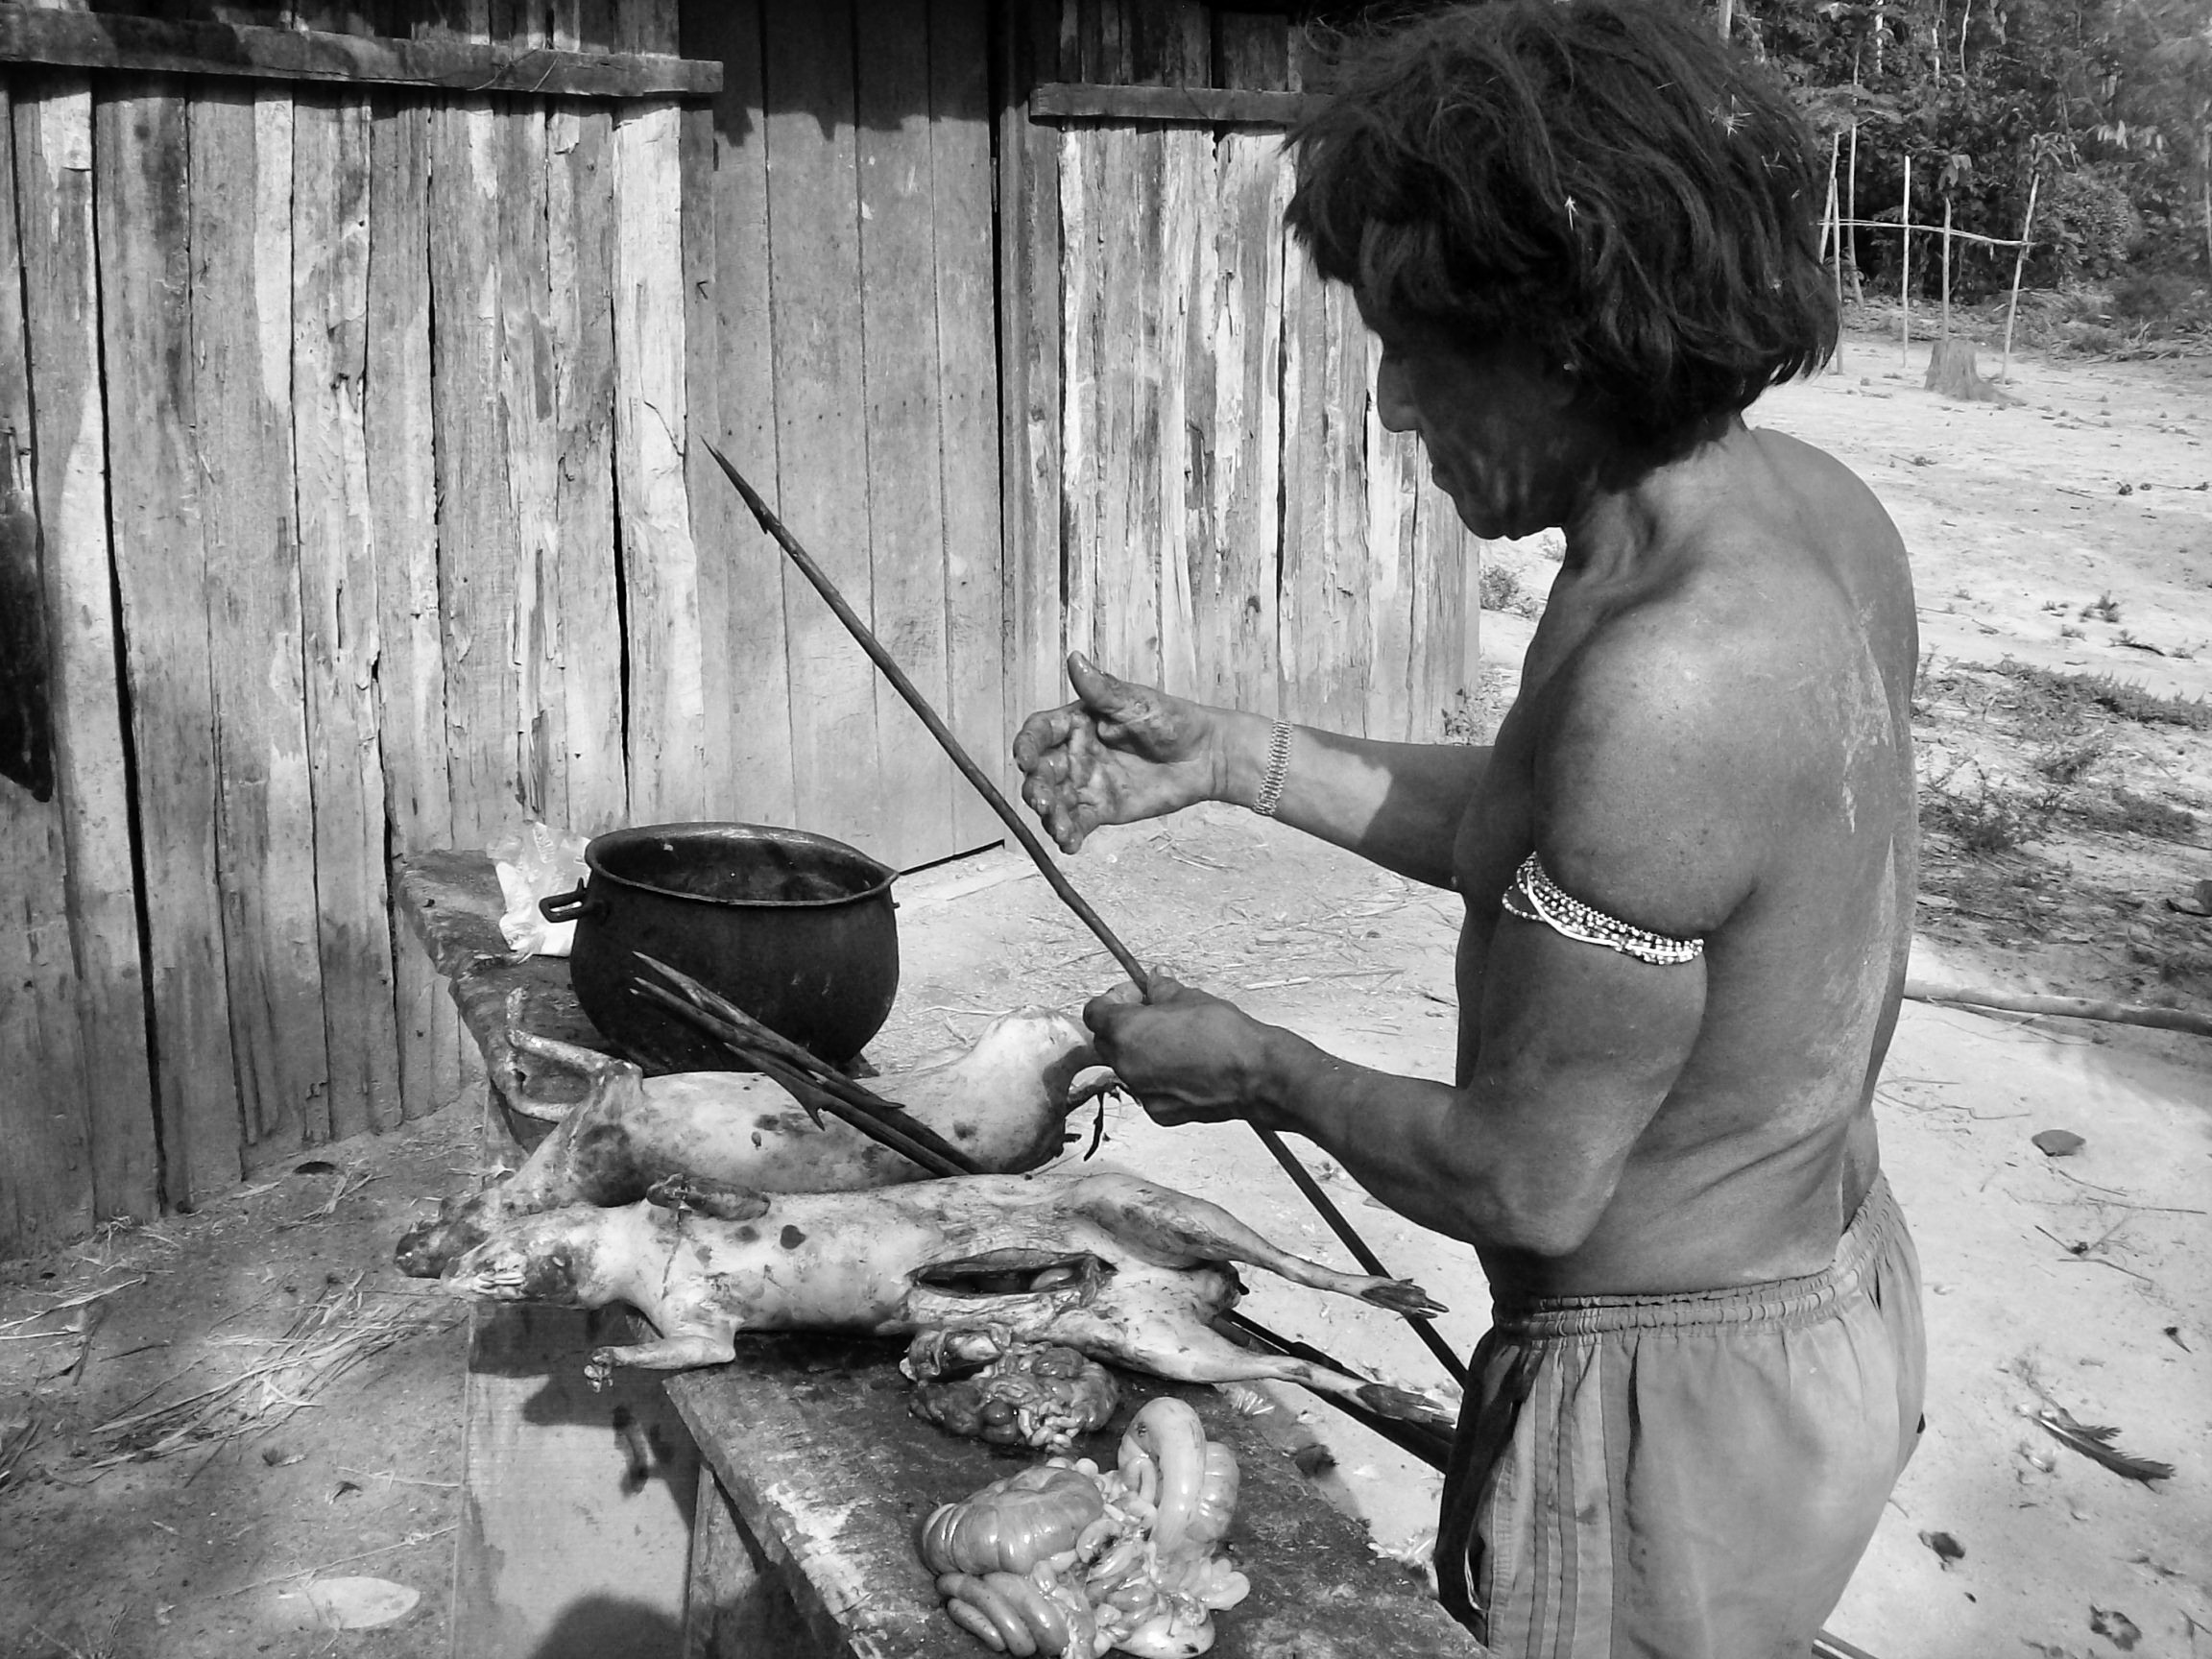
\includegraphics[width=\textwidth]{./imgs/100_5107}
%\caption{Kamaraxa’a alimentando e conversando com suas flechas (aldeia Juriti, 2009).}
%\end{figure}

Assim como ocorre aos humanos durante a caçada, as flechas e tabocas
também devem entrar em um estado de ``raiva'', \textit{imahy}, para que
funcionem de maneira adequada. Para que desenvolva ``raiva'' é necessário
que os homens lhe forneçam dois elementos cruciais à saúde da flecha:
``dor'', \textit{hahy}, e ``sangue-veneno'', \textit{hawy}. Por isso, após
confeccionada, uma flecha ainda não está pronta para o uso, pois requer
um longo processo de ``alimentação'' e ``envenenamento'' de modo a se
fortalecer e, com isso, aí sim, ser capaz de matar. ``As flechas têm
fome, por isso caçamos muito!'', disse-me certa vez o velho Takya, um
desses homens que caçam exclusivamente com arco e flechas. Uma flecha se
alimenta fundamentalmente do sangue de suas presas. Uma vez um animal
morto, os homens esfregam na carne cheia de sangue as pontas de diversas
flechas para que, assim, a fome delas seja aplacada. O sangue animal é
dito ``alimento'' --- \textit{hami'ũa}, ``comida dela'' --- para as flechas, ao
mesmo tempo que é o ``veneno'', \textit{hawy}, que elas lançarão nas presas
animais. O banho de sangue é a primeira etapa do processo de
transformação da flecha objeto-em-si em uma arma mortífera, repleta de
``dor'' e ``raiva'', que será despejada nas presas animais, causando sua
morte. Uma nova flecha, após confeccionada, tem suas pontas revestidas
de sangue e se zanga caso não se a alimente, o que pode fazer com que
não funcione ou que vá contra a vida de uma pessoa; por isso,
fornecem-lhes o sangue desejado, para que fiquem boas, \textit{katy}.
Certa vez, após uma caçada de macacos, um dos cuxiús estava derramando
bastante sangue e, enquanto descansávamos antes de retornarmos à aldeia,
Takya esfregava suas flechas no corpo ensanguentado do animal.

É comum os homens, enquanto estão limpando as caças, levarem junto
algumas flechas para esfregar no corpo do animal após aberto, antes de
destripá-lo e lavá-lo. Nessas ocasiões, eles podem, inclusive, conversar
com as flechas, pedindo que elas voltem a matar e que, por isso, as está
alimentando. Os homens também observam que as flechas não param de lhes
pedir sangue. Caso não atendessem a esses incessantes pedidos, elas não
matariam nenhum animal --- se quebrariam ou não acertariam o alvo. Takya
diz que ``conversa'' com suas flechas, pois elas mesmas lhe pedem sangue:
``Me dá \textit{hawykera}, 'sangue''', ``eu quero \textit{hawykera}, se você me
der eu terei sangue-veneno para pegar mais carnes, matar mais bichos. Eu
envenenarei outros animais para você!'' (assim, segundo o velho Takya,
suas flechas falariam). Questionei-o a respeito de como se dava essa
``comunicação'' entre caçador e flecha. Ele simplesmente respondeu-me que
é uma coisa que ``os Guajá sabem fazer'', \textit{awa} \textit{kwa}.

Trata-se do único uso que fazem do sangue animal, dito extremamente
venenoso (as mulheres não podem sentir sequer o cheiro do sangue de
alguns animais como o veado). Para as flechas, o sangue é como um
remédio, \textit{pohỹ}, enquanto que para os Guajá, ele é um veneno, me
disse certa vez Wirahoa. Devido a tal capacidade letal, ``sangue'' e
``veneno'' são referidos pela mesma palavra na língua guajá, \textit{hawy};
o veneno de uma cobra é chamado de \textit{hawy}, bem como o sangue que
escorre de uma ferida humana é \textit{hawy}. Em uma taboca se passa o
sangue de animais grandes, como caititu, queixadas e antas, e o desta
última é extremamente benéfico, pois, de maneira mimética, produz na
taboca uma ``dureza'' análoga à do couro de anta: quase indestrutível. Por
outro lado, os animaizinhos pequenos, do tipo que os Guajá não caçam,
como o esquilo caxinguelê, \textit{tamakaja}, ou mesmo ratos, 
\textit{awijỹa}, não são possíveis presas na perspectiva de uma flecha.
Certa vez, de forma um tanto irreverente, um homem me afirmou que tais
animais são \textit{maka} \textit{nimá}, \textit{kĩ nima}, e \textit{wy'y}
\textit{nima}, ou seja, animais de criação das espingardas, tabocas e
flechas; por isso as armas não os matam.

As únicas restrições sanguíneas postas a uma flecha são o sangue de uma
onça-pintada, \textit{jawaruhua}, e o sangue humano (não só dos Guajá, mas
qualquer humano: \textit{awa}, \textit{mihua}, \textit{kamara} ou
\textit{karaia}). O sangue humano é altamente nocivo a uma taboca, e caso
uma dessas flechas venha a matar algum humano ela deve ser imediatamente
descartada, pois corre-se o risco de uma taboca se acostumar ao sangue
dos humanos e passe a querer sempre mais (voltaremos a esse ponto). Já o
sangue da onça-pintada (alguns afirmaram) é inapropriado para uma taboca
pois a enfraquece; nesses casos é necessário limpar as ponta da taboca
antes de a colocar novamente em uso --- mas não é necessário descartá-la.
Essa regra não se aplica à sussuarana (ainda hoje considerada uma
possibilidade alimentar) ou à jaguatirica (que não comem), cujos sangues
também são alimento para as flechas e tabocas. Uma flecha só é jogada
fora caso se quebre, se torne imprestável ou mate um humano.

O sangue, por ser um ``veneno'', atuaria aqui como uma espécie de
\textit{curare},\footnote{\textit{Curare} é um termo genérico que se refere
  aos venenos de caça utilizados por diversos povos ameríndios e, dessa
  forma, ``cobre uma multiplicidade de preparações tóxicas diferentes,
      geralmente à base de plantas do tipo \textit{Strychnos}'' (Descola, 1996, p.
  309).} veneno utilizado nas pontas de projéteis de caça por diversos
grupos ameríndios. No caso Ashuar --- um povo que caça com zarabatanas ---
Descola observa que, ao preparar seu \textit{curare} na floresta (entre os
Ashuar é chamado \textit{tseas}), quando cozinham as plantas lentamente,
longe das mulheres e da aldeia, os homens cantam alguns
\textit{anent}\footnote{\textit{Anent} é uma encantação cantada, utilizada
  em todas as circunstâncias da vida cotidiana e ritual Ashuar, a fim de
  alcançar algum resultado desejado ou conquistar os favores de um
  destinatário (Descola, 2006, p.\,495).} para fortalecer o preparado. Tais
encantamentos se dirigem diretamente ao \textit{tseas} (\textit{curare}) de
maneira vocativa, eles lhe ordenam que beba o sangue dos animais contra
os quais será empregado, e cada espécie de caça é nomeada, uma após
outra (Descola, \textit{op.\,cit.}, p.\,310). A fabricação de \textit{curares}, entre
os Ashuar, por exemplo, exige um rigor (distância completa das mulheres;
abstinência sexual; saída da aldeia e reclusão na floresta) que é
ausente no processo de ``envenenamento'' das flechas Guajá. Porém,
enquanto os Jívaro sustentam ser um envenenamento-encantamento com o
curare durante a preparação das setas da zarabatana --- uma vez que os
encantos \textit{anent} são fundamentais para o bom funcionamento dessas
setas --- os Guajá afirmam que o sangue --- \textit{hawy}, ``sangue-veneno'' ---
produz um mesmo envenenamento nas flechas. Muito embora não haja
``encantamento'', como não há em coisa alguma na vida cotidiana e ritual,
os homens também conversam com suas flechas enquanto as preparam. Essa
conexão entre o sangue consumido e uma boa flecha ocorre mesmo no
aprendizado do manuseio durante a infância. Certa vez o pequeno
Makoraia, que na ocasião tinha apenas cinco anos, atirava em grilos e
calangos que vivem pela área da aldeia e seu entorno as flechinhas
feitas por seu irmão mais velho. Após matar os camaleões, duas de suas
flechas ficaram com a ponta lambuzada de sangue, e ele comentou, rindo,
que deixaria daquele jeito pois é assim que fazem os Guajá.

Quanto ao veneno de caça, a partir de um mito Kachuyana sobre a origem
do curare, (cujo veneno foi dado aos humanos pelo gavião-real; por isso,
o cipó utilizado por esse povo para o produzir é chamado ``flecha do
gavião-real''), Lévi-Strauss argumenta que, nesse caso, o curare,
utilizado basicamente para matar ``macacos coatás'', é besuntado nas
flechas com um pincel de pelos de capelão (Lévi-Strauss, 2004, p.\,315).
Lévi-Strauss mesmo, indagando o lugar sutil dos venenos de caça nas
culturas ameríndias, indica que ele atua como uma ``intrusão'', uma das
raras situações em que a natureza se aproxima da cultura a ponto de
quase determiná-la. Em uma linguagem musical, os venenos se dispõem em
um curto intervalo cromático que --- diferentemente de quase todo
pensamento ameríndio, afeito aos grandes intervalos descontínuos
(diatônicos, portanto) --- faz com que um produto estritamente natural (o
veneno) sirva a uma atividade cultural, a caça (Lévi-Strauss, \textit{op.\,cit.},
p.\,321. Ver também Descola, 1996, pp.\,310--311). Penso que podemos incluir
o sangue das flechas Guajá nesse mesmo conjunto, pois, com exceção de
seu envenenamento, o contato com o sangue é evitado em todas as
situações devido a sua nocividade animalesca. Como se um elemento
pertencente a uma ``extrema'' natureza (diferentemente da carne que é
cozida e consumida enquanto o sangue é lavado e descartado) fosse
desnaturalizado --- ou mesmo culturalizado --- e transformado em veneno.

\begin{center}\adforn{68}\end{center}

Após uma flecha ou taboca ser alimentada de sangue-veneno, ela deve
tornar-se forte, dura, \textit{hatỹ}. Para isso é posta em um jirau
situado estrategicamente acima do moquém, preso às vigas do teto de um
casa, para que o fogo seque o sangue e a defume, \textit{tataxĩa}. Esse
processo faz com que a flecha assuma uma tonalidade marrom, bem escura
(como pó de café), tendendo para o preto. Quando ela alcança essa cor é
sinal de que está pronta para o uso, capaz de despejar ``veneno'' e ``dor''
em qualquer ser vivente. O objetivo da defumação das flechas é fazer com
que fiquem repletas de \textit{hahy}, ``dor''; é isso que magoa a ferida e
provoca, consequentemente, a morte das presas animais. Como acontece
também com as flechas Yudjá, para os Guajá ``as flechas de caça devem
ser sobredotadas do poder de causar dor: \textit{Sem isso a flecha não
mata nada!''} (Lima, 1995, p.\,110). Tanto a taboca quanto a flecha se
alimentam de sangue, fortalecem-se com ele; e a fumaça, \textit{tataxĩa},
além de lhes dar firmeza, as envenena. Uma combinação explosiva.

É importante atentar para a relação entre a fumaça do fogo de cozinha e
os usos benéficos desse elemento. A mesma fumaça que é fundamental no
processamento da carne em alimento (pois a carne é defumada: assada pela
fumaça) endurece e fortalece as flechas (colocando ``dor'' nelas). A
fumaça do fogo de cozinha, dizem os Guajá, retira o sangue dos animais e
endurece a carne para que os humanos possam comer. Ela tem uma função
endurecedora, sendo essa, inclusive, uma das definições de ``culinária''
para os Guajá: o endurecimento da carne e eliminação do sangue. Ao mesmo
tempo que endurece, ela fortalece, e os Guajá imputam tal propriedade à
ação da fumaça. Por exemplo, quando um bebê começa a dar seus primeiros
passos, seus pais e irmãos mais velhos, de forma muito carinhosa,
realizam um procedimento chamado \textit{kytykyty}, ``esfregar'', que
consiste em ``pegar'' a fumaça produzida pela fervura de uma panela, ou da
queima de uma lenha, e esfregar nos joelhos de um bebê, como se
introduzissem a fumaça no corpo da criança para que suas articulações se
enrijeçam --- \textit{hatỹ}, ``ficar duro'' ---, tal como ocorre com a carne
posta a moquear e com a flecha posta a endurecer. Aqui, a fumaça
endureceria as flechas e os ossos, \textit{ikaena}.\footnote{Quando se
  está cansado, inclusive, são os ossos, \textit{ikaena}, que estão
  cansados, doloridos, e por isso precisam descansar.}

O efeito dos projéteis (sejam flechas ou chumbo) sobre os animais,
aquilo que os faz morrer após serem alvejados, se baseia na teoria Guajá
de que tais peças são carregadas de dor, \textit{hahy}, e veneno, 
\textit{hawy}. Enquanto o sangue a alimenta, envenenando-a para que
lance esse veneno em suas presas, é a fumaça que insere \textit{hahy}, ``dor'', 
na flecha. Tal procedimento faz com que um animal se fira
gravemente e que a dor e o veneno da flecha sejam transferidos
(``cuspidos'', dizem os Guajá) para ele. Após a presa ser alvejada, a dor
que permanece na ferida (chamada \textit{ha'ina} --- uma espécie de
``bichinho'', me disse um amigo guajá) é que faz o machucado doer,
reforçando a tese de que a dor é sempre externa, algo que é posto de
fora para dentro. Certa vez, alvejaram com espingarda uma cobra surucucu
pico-de-jaca, \textit{arikukua}. Abatida instantaneamente, ela foi
``comida pelo chumbo'', um elemento que, tal como as flechas, é faminto
por sangue e portador de muita dor.

O fator complementar (e indispensável) que torna as flechas seres
completamente devastadores e replenos de desejo homicida é a plumagem
escolhida. As penas utilizadas em uma flecha, ainda em sua confecção
inicial, devem ser preferencialmente de aves de rapina (diversas
espécies de gaviões ou harpia) ou mesmo de urubus, porque, de acordo com
a tecnologia Guajá, a plumagem dessas aves tem \textit{hawy}, ``sangue-veneno'', 
já que seus portadores originais se alimentam de carne
e sangue. Para além disso, os Guajá --- de maneira a me traduzir e
simplificar suas ideias --- dizem que os gaviões, por exemplo, aceitam
esse ``acordo'' com os humanos e gostam que suas penas sejam utilizadas
para matar outros animais. Além das penas que gostam de sangue, ainda
utilizam outras excelentes, como de jacu, mutum e até mesmo araras,
embora, lembro-me, prefiram sempre as de gavião --- \textit{wiraho}
\textit{popokera}, ``penas do que foi um gavião'' ---, que por si só são
impregnadas de sangue-veneno, o que é tão saudável para uma flecha
quanto o sangue espalhado em suas pontas.

É com uma dedicação exemplar que os Guajá cuidam de suas flechas, das
espingardas e da montagem de seus cartuchos. Esses últimos, inclusive,
também se distinguem em relação aos mais preferidos, tal como são as
flechas (umas melhores que as outras). Uma flecha que tenha matado
macacos-pregos, na caçada seguinte desses animais e após reparada, será
certamente utilizada de novo. E assim sucessivamente. É como se os
objetos fossem se especializando por eles mesmos. Como se a ação do
objeto se manifestasse a partir de sua eficiência. Ao fazer suas
flechas, é comum seu artesão já saber qual será a finalidade de cada
uma, em que animal ele fará com que cada uma se especialize. Certa vez,
o velho Pirama'ã confeccionava suas flechas, \textit{wy'ya}, quando
começou a conversar com Juwi'ia, um de seus netos mais velhos, e lhe
mostrou o que faria com cada uma delas, sugerindo um caráter
exclusivista na utilidade de cada uma. Ele dizia: ``Esta vai para o
capelão, esta outra para o inhambu, esta, para o macaco-prego, e esta,
para o poraquê'' --- enquanto seu neto (que já era grande) ria e olhava
atentamente, ao mesmo tempo que, para me incluir na conversa, repetia em
português o que o avô estava dizendo. O falecido Pinawãxa'a certa vez
mostrou-me um cartucho, \textit{jamekera}, que, com ele, havia matado ---
com um único tiro --- dois capelães de uma vez; e teceu vários elogios ao
objeto. Em outra ocasião, Pirama'ã estava caçando capelães e, após
atirar, \textit{japi}, e errar, passou boa parte da tarde procurando pela
flecha usada. ``Era uma boa flecha'', \textit{wy'ya} \textit{katy}, me disse,
percorrendo uma grande área, até por fim encontrá-la. Mesmo com centenas
de flechas em seus feixes, uma ``boa flecha'' não pode ser desperdiçada,
pois ela é fruto (muitas vezes) da antiga relação entre si e seu dono, 
\textit{jara}.

Para se referir às espingardas e cartuchos, os Guajá recorrem às mesmas
ideias que definem suas flechas, porém, com mais intensidade. Loucas, 
\textit{waky}, raivosas, \textit{imahy}, inimigas, \textit{mihua}, dentre
outros adjetivos, servem para definir as espingardas e os cartuchos. Os
cartuchos são ditos incontroláveis. Diferentemente das flechas, eles
matam tudo; até filhotes que se poderiam tomar por animais de criação.
Antes de caçarem com espingardas, matavam-se muito poucos filhotes
(ainda muito pequenos) de qualquer animal, pois as flechas gostam dos
animaizinhos \textit{nima} (como me disse certa vez Hajmokoma'ã). Por
outro lado, os cartuchos são ``doidos'' e matam tudo. Certa vez, em uma
caçada de capelães havia dois filhotes: um que sobreviveu intacto, e
outro que, alvejado na perna, morreu antes de voltarmos para a aldeia.
Todos disseram que foi o cartucho que o matara; que os cartuchos têm
muito veneno e raiva; e são doidos --- diferentes das flechas, que sabem,
\textit{kwa}, mais.

Outra vez, em uma das reuniões com membros do \textsc{cgiirc}, quando os Guajá
discutiam a necessidade de uma política a favor da compra e manutenção
de armas de fogo --- frente ao Estatuto do Desarmamento brasileiro, que a
Funai aplica desde a Lei Nº 10.826 de 2003 quando se instituiu o Sistema
Nacional de Armas no Brasil\footnote{Veja, no site do Planalto, o texto completo da Lei Nº 10.826. Um problema central em todas as aldeias é a
  falta clara de uma política para a compra de munição e a manutenção
  das armas de fogo entre este povo, cuja subsistência e economia
  simbólica é dependente da caça. De tempos em tempos seu debate volta à
  tona, com imagens que evocam um ``faroeste''; sugerindo que os
  indígenas não teriam a competência ou preparo psicológico para
  utilizar armas de fogo. Visto que esses povos são, grosso modo,
  considerados um empecilho ao desenvolvimento, capazes de atacar
  colonos e frear o avanço da fronteira com seus arcos, flechas e
  bordunas, o uso de espingardas torná-los-ia ainda mais perigosos. Para
  outros, a introdução de novas tecnologias nas comunidades indígenas os
  ``viciariam'' ao ponto de incentivá-los a abrir mão de seus
  conhecimentos tradicionais, além de propiciar o rápido esgotamento dos
  recursos naturais em suas áreas. Não compartilho com nenhuma das duas
  posições, defendo que para um povo como os Guajá, a partir de uma
  série de pontos e reflexões que estamos vendo no decorrer deste livro,
  a caça com armas de fogo é uma alternativa sustentável e indispensável
  à vida deles, dado o ganho econômico oriundo de sua utilização.} ---; ao
tentar convencê-los dos perigos de caçar com espingarda, um
representante da Funai argumentou que as armas, além de tudo, eram
perigosas, pois as pessoas eventualmente podem matar umas às outras com
elas, e os brancos, \textit{karaia}, que se matam com armas, são a melhor
prova disso. Um dos representantes guajá fez então uma breve fala;
lembrou que os brancos só morrem nas mãos das armas de fogo porque
atiram um nos outros com elas, e que os Guajá, por não atirarem flechas
uns nos outros, não morrem pela flecha, e muito menos isso aconteceria
com as armas de fogo. Lembrou também que o uso que fazem de arma de fogo
é, por incrível que possa parecer, ainda menos letal que o uso que fazem
das flechas. Esse jovem líder, chamado Itaxĩa, enumerou um razoável
conjunto de casos de pessoas que haviam sido atingidas por flechas
desgovernadas ou que caíam no lugar errado, enquanto que com as armas de
fogo acidentes como esse nunca aconteciam. Em poucas palavras, de forma
perspicaz --- ao menos para mim --- Itaxĩa estava argumentando que, da
maneira que os guajá utilizam suas armas de fogo, elas são menos
perigosas do que flechas e tabocas.

A crise que os Guajá enfrentam hoje, pela falta de munição é concebida
por eles como fruto de uma esquizofrenia política do estado brasileiro,
em particular, da Funai. Todos conseguem relembrar a chegada das
espingardas nas aldeias: do barulho, o estranhamento, o cheiro de
pólvora e, sobretudo, o rendimento econômico que essa nova tecnologia
proporcionou à ``boa vida'', \textit{iku katy}, humana. As chamadas
``\textit{Vinte}'' (espingarda de calibre 20) entraram na caça Guajá logo
nos primeiros dias de contato, porém hoje as pessoas não podem comprar
munição, muito menos novas espingardas, pois é proibido por lei. Os
Guajá não entendem por que foram convencidos a escolher a espingarda no
lugar de suas flechas há poucas décadas, ficando completamente
dependentes da caça com armas de fogo, e a mesma Funai que lhes
possibilitou essa transição diz que não podem mais possuir suas armas
nem comprar a munição.

\begin{center}\adforn{68}\end{center}

Passar sangue nas flechas, como estamos vendo, é um processo alimentar e
de envenenamento. Hoje, os Guajá chamam essa operação de ``lustrar'' (em
português). Da mesma forma que lustram suas espingardas com o óleo de
máquina, lustram suas flechas com sangue. Tal como uma flecha tem fome
de sangue, uma espingarda, \textit{maka}, tem fome de óleo. O ato de
lustrar a espingarda parece produzir na arma um efeito análogo ao
alcançado quando lustram as flechas com sangue. Assim, para a arma, o
óleo produz o mesmo efeito alimentar que o sangue produz nas flechas,
fazendo com que fique forte e com raiva, ao mesmo tempo que aplaca sua
fome. Lembro-me de, nos meus primeiros dias na aldeia Juriti, reparar
que todos os homens passavam boa parte do dia desmontando as
espingardas, até suas mínimas peças, e tornavam a montar, as limpavam e
lustravam. Isto ocorria quase que diariamente, da mesma forma que os
velhos fazem com as flechas; não só as reparam, mas também as alimentam
e criam, \textit{riku}, como garantem ser a relação de um caçador e sua
flecha (voltaremos a esse ponto).

De tanto montar e desmontar, as armas são repletas de remendos e
adaptações e constantemente voltam a quebrar. Muitas vezes os defeitos
são provocados por essa extrema manutenção diária, e não pelo uso
intenso, propriamente. Isso gera comentários infelizes por parte de
alguns funcionários do Posto Indígena, em um jogo de ataques e defesas
entre os próprios funcionários. Alguns criticam que os homens são
incapazes de possuir uma espingarda sem as quebrar ou que as armas só se
quebram porque ``mexem'' muito nelas. Outros os defendem, dizendo que as
espingardas se quebram porque seu uso é o ``ganha-pão'' deles; que eles
precisam utilizá-las muito mais do que os ``brancos'', e por isso elas se
quebrariam tanto. O fato é que há uma total dependência dos Guajá em
relação à Funai para a compra de munição e o reparo das espingardas
(quando precisam de reposição de peças) --- o que nem sempre dá certo. A
maior parte de minhas reservas financeiras foram repassadas para comprar
munição (artigo muito caro) e pagar reparos de espingardas, a pedido dos
Guajá ou dos próprios funcionários da Funai (no caso do reparo de
espingardas, funcionários chegavam a me pedir ajuda, pois a
administração da Funai dificilmente paga reparos). Com suas espingardas
quebradas, os homens ficam muito apreensivos, pegam emprestadas as armas
de seus irmãos que, devido ao uso intenso, também podem se quebrar. E
isso seria uma espingarda a menos na aldeia. As espingardas (e
principalmente a munição) são o principal assunto entre os homens e os
funcionários do posto. Para estes, os Guajá utilizam mal a espingarda,
para os Guajá, os funcionários são sovinas, pois teriam acesso a uma
grande quantidade de munição com os \textit{karaia} das cidades, mas
regulam e não a fornecem na quantidade adequada.\footnote{Só para termos
  uma ideia, a munição foi a única exigência colocada pelos Guajá de
  todas as aldeias, quando solicitei autorização de pesquisa à Funai. Em
  2007, ao chegar pela primeira vez na aldeia Juriti, por ter comprado a
  munição na companhia de um funcionário da Funai ele pediu-me que a
  deixasse com ele, pois os Guajá ainda tinham um pouco em suas casas, e
  se eu distribuísse tudo de uma só vez eles a consumiriam rapidamente.
  Argumentei então que daria ao menos uma parte para que as pessoas
  vissem que eu havia trazido o que elas me pediram. Foi o que fiz, sem
  maiores problemas. Ao me perguntarem se eu havia trazido mais do que
  aquela pequena quantidade que distribuía, informei-lhes que o chefe de
  posto havia retido uma parte da munição que eu havia levado para lhes
  dar em outra ocasião, quando precisassem novamente. Com isso, ficaram
  chateados comigo dizendo que, da próxima vez que eu os visitasse,
  desse toda a munição a eles, diretamente. Assim o fiz na minha segunda
  viagem, em 2008. Ao retornar à aldeia Juriti, comuniquei ao chefe do
  Posto que entregaria a munição diretamente aos homens, pois eles assim
  haviam me pedido. Um pouco contrariado, o funcionário aceitou minha
  proposta. Ao distribuir a munição aos homens eles me pediram que eu
  desse somente metade a eles e entregasse a outra metade ao chefe de
  posto, para que ele guardasse melhor e depois distribuísse mais um
  pouco. Eu insisti que não, que pegassem tudo, pois seria melhor para
  eles. No entanto, me asseguraram que ainda tinham alguma munição
  guardada em suas casas e que, por isso, era melhor armazenar esse
  excedente na sede do posto. Quando precisassem, solicitariam ao chefe
  de Posto.}

Além do óleo, os homens me pediam que comprasse tinta de metal da cor
preta para pintarem os canos e as partes de metal de suas espingardas.
Segundo me explicou Wirahoa --- nessa teoria Guajá sobre as armas (e o
metal) ---, o cano da espingarda (originalmente metálico ou dourado),
estando na cor preta, ``enxergaria'' melhor a caça, tal como ocorre com as
flechas ``defumadas'' que, enegrecidas, aguçam sua ``visão'' e potência.
Como vimos, após sangradas e defumadas, as flechas ficam escuras, como
se fossem queimadas, e por não poderem fazer o mesmo com a espingarda
(deixar em cima de um moquém), pois a estragariam; a tinta preta
produziria o mesmo efeito, faria com que ela se tornasse mais eficiente.

\section{objetos inimigos são domesticados}

As tabocas e as flechas são ditas serem \textit{mihua}, ``inimigas'',
``selvagens'', que, como vimos, é também o termo pelo qual classificam
diversos grupos distantes, com os quais mantêm relações de inimizade em
potencial, os ``Guajá brabos'', como costumam dizer. Wirahoa diz que no
processo comunicacional entre as flechas e seus donos elas falam: ``Me
coloque no fogo quente!\ldots{} Isso mesmo, mais quente, mais quente!\ldots{} e
agora me levem para matar porcos''. Por isso, se forem bem defumadas
matarão suas presas animais com mais facilidade, como se seu
veneno-sangue, \textit{hawy}, estivesse muito ativo. Ainda segundo
Wirahoa, quando uma flecha está no arco, prestes a ser atirada, \textit{japi}, é como se ela dissesse ao animal: ``Eu sou \textit{mihua}, `braba', 
não sou seu \textit{harapihiara}, ``cognato'', ``parente próximo'',
não sou sua amiga, \textit{aty}, eu só gosto dos \textit{awa}, humanos,
pois eles cuidam de mim, \textit{riku}, me alimentam\ldots{} por isso eu vou
te matar!'' Portanto, as flechas são inimigas, criadas para serem assim.
Mas, por serem domesticadas pelos humanos, mesmo sendo ``brabas'' quase
nunca os atacam, ao contrário do que ocorre com o chumbo, 
\textit{maka'ina},  dos cartuchos, \textit{jamekera}, que não obedecem a
ninguém, são ``doidos'', \textit{waky}.

Vimos no capítulo anterior que os Guajá desenvolveram uma forma de
anulação da distância cognática (se assim podemos pensar) a partir da
ideia-relação \textit{riku}. Da mesma maneira que o \textit{riku} funciona
entre diversos seres, os muitos agenciamentos entre um caçador e suas
flechas e tabocas são da ordem de uma relação \textit{riku}. Fabricá-las é
só um primeiro passo para as possuir. E ninguém possui uma flecha só
porque a fabricou, pois possuí-las é obrigatoriamente ``criá-las'', 
\textit{riku}. Muito embora essas armas de caça e guerra sejam feitas
(como objetos) pelos humanos, têm uma autonomia a ponto de seus donos
manterem com elas uma relação \textit{riku}. Em outras palavras, como
sempre me foi traduzido, os homens ``criam'' suas flechas, e criá-las
implica basicamente confeccioná-las (obviamente, porém com as penas
certas), alimentá-las e repará-las sempre que necessário --- um processo
constante e de longa duração. Por serem perigosas, \textit{mihua},
somente a domesticação, \textit{riku}, pode lhes proporcionar uma vida
proveitosa (sem acidentes e tragédias), sendo que parte da destreza do
caçador está na qualidade dessa relação estabelecida com seu feixe de
flechas. As flechas e tabocas agem intencionalmente: se não desejarem
funcionar não funcionam (quebram, erram o alvo, se perdem). Por isso
elas estão no \textit{hall} dos ``seres domesticáveis''. Por agir com
intenção e vontade, algumas flechas e tabocas se prestam a matar alguns
animais de forma mais eficiente do que outras, e algumas delas são
excelentes companheiras de caça. Em seu arsenal domiciliar, aqueles
homens que não fazem uso de espingarda contam, em média, com 200
projéteis, entre flechas e tabocas.

Quando saem para a mata, carregam de 15 a 30 projéteis formados em um
feixe, precisamente amarrados por um cipó e com as pontas em conjunto
envoltas por uma folha larga de palmeira, tal como uma delicada
embalagem protetora. Esse cuidado se justifica, pois garante que as
pontas afiadas não trisquem em nada e não sejam avariadas durante as
longas caminhadas. Firmeza, retidão, fio adequado, dentre tantos fatores
técnicos, são levados em conta para que uma flecha esteja o mais próximo
da perfeição. O velho Pirama'ã, um exímio arqueiro, uma vez na mata,
antes de subir numa árvore atrás de capelães ou se embrenhar por um
brejo à procura de um poraquê, seleciona, de seu feixe, as flechas que
realmente lhe serão úteis: morde-as, entorta-as, confere a plumagem e\ldots{}
conversa com elas: tarefas importantes, feitas com concentração. No
entanto, como quase tudo na vida cotidiana dos Guajá, essas ações
ocorrem sem nenhum cerimonialismo. Ele apenas deve se certificar de que
são as flechas certas para ``estar com'' ele, \textit{riku}. As flechas são
aproveitadas até se esgotarem. Só são descartadas quando se quebram
completamente.

Embora eu não tenha coletado nenhum mito específico sobre a origem das
flechas e seus usos, sei que, para os Guajá, \textit{Maíra} possuía
flechas mágicas que, ao invés de tirar, davam vida aos seres. Como
exemplo, após \textit{Maíra} ter transformado uma pedra na primeira anta, 
\textit{tapi'ira}, ele atirou uma de suas flechas na anta-pedra e ela
saiu correndo na forma de anta; e quando transformou um cupinzeiro no
primeiro queixada fez o mesmo. Há, na verdade, duas interpretações para
o procedimento de \textit{Maíra} nesses feitos magníficos. Um é que ele
apenas gritou ``Vá, anta!'' --- \textit{awyhy!}, ``corra''; e o outro ao atirar
flechas mágicas, também gritando ``Vá, anta!'' Com exceção de episódios
como esse, não encontrei na mitologia guajá
histórias específicas sobre flechas. No entanto, a mitologia ameríndia é
repleta de episódios que as apresentam como seres-objetos repletos de
desejo, intenção e autonomia: flechas especializadas em caças
específicas e mesmo algumas que caçam sozinhas estão presentes, de uma
forma geral (no último capítulo, veremos como são as flechas dos
\textit{karawara}, energizadas, com que caçam na Terra). Há um mito
Karajá, apresentado por Lévi Strauss (\textsc{m}177), sobre um caçador que obtém
a proteção de uma rã em troca de carícias ilusórias e que se torna ``um
caçador milagroso, graças a zagaias dadas por ela (a rã), `uma para
cada tipo de alimento', cuja força é preciso atenuar
besuntando-as com um unguento, que equivale, portanto, a uma espécie de
veneno de caça invertido'' (Lévi-Strauss, 2004, p.\,197). Veremos adiante
como os \textit{karawara}, de alguma forma, representam um certo ideal de
caça guajá que prescreve tal exclusividade: de um tipo de caçador para
um tipo de caça, tal como uma flecha específica para uma caça específica
--- como quis mostrar-me Pirama'ã (relacionando suas flechas aos animais
que elas preferencialmente vão matar) e como encontramos na mitologia
ameríndia.\footnote{Ver \textsc{m}177 em Lévi-Strauss, 2004, p.\,197.}

Em outros casos analisados por Lévi-Strauss, em dois mitos Toba (\textsc{m}212 e
\textsc{m}213), sobre a ``moça louca por mel'', há uma referência a ``flechas
mágicas'' lançadas por um pica-pau que, ao notar o sumiço de sua esposa,
dispara-as em várias direções para que procurem a mulher desaparecida.
As flechas não obtêm sucesso e voltam sozinhas até seu dono, assim, ele
percebe que sua mulher não foi encontrada por suas flechas (em uma das
versões, \textsc{m}212, uma flecha a encontra e as outras retornam ao dono). Há
outros mitos sobre flechas muito precisas, que conseguem acertar o meio
de um fino cipó; ou ainda, se lançadas ao alto, ao cair acertam em cheio
o dorso de um animal; dentre outras. Há ainda um mito Waiãpi, coletado
por Gallois (1988), sobre a origem das flechas e dos acidentes com
flechas que sustenta que, antigamente, quando os caçadores lançavam suas
flechas, eles diziam a elas: ``volte flecha, pode voltar''. Eis que as
flechas falavam: ``cuidado, se afaste eu vou descer''. Hoje, as flechas
não falam mais e podem acertar qualquer um. Isto posto, da mesma forma
os Guajá gostam de pensar que cada uma de suas flechas tem predileção
especial por determinado animal, nunca falado de forma explícita, mas na
prática eles selecionam flechas com ``histórico'' de predações
específicas. Pois, uma flecha que já matou muitos macacos-pregos
continuará sendo utilizada para matar macacos-pregos; e assim
sucessivamente, como se a ação fosse imanente ao objeto, independente do
caçador.

Para finalizar este capítulo, em que busquei descrever aspectos técnicos
das atividades de caça, lembro que se a mesma taboca que assassinou um
humano for reutilizada em outra caçada, tempos depois, ela certamente
desprezará o alvo e se voltará contra aqueles que estiverem ao redor do
caçador, em busca de mais sangue humano. Por isso, uma taboca que já
experimentou desse sangue deve ser inutilizada.\footnote{Isso faz lembrar
  o citado mito Karajá (\textsc{m}177, Lévi-Strauss, 2004a: 353) em que o caçador
  consegue flechas mágicas para destruir ``uma raça de macacos canibais,
  da espécie guariba'', porém as flechas são tão venenosas que o caçador
  precisa enfraquecê-las (desenvenená-las) com o tal unguento mágico
  pois, caso contrário, ela se voltaria contra o próprio caçador.} Algo
semelhante ocorre com o próprio matador de guerra Guajá (bem como outros
casos Tupi), que aqui absorve a raiva, \textit{ha'aera}, (não o sangue) do
inimigo e se torna perigoso à vida na aldeia, um quase-inimigo (como
sabemos, a partir também do já clássico caso Araweté, Viveiros de Castro
1986). Por isso, tanto um matador quanto uma taboca assassina
representam ambos uma ameaça real para toda a vida da aldeia e, por
segurança, a taboca que se alimentou de sangue humano deve ser
descartada, enquanto quem matou cumpre um resguardo.

Devo aqui lembrar que na Amazônia a taboca é parte constituinte (e
central) de muitos arsenais de guerra; peça-chave em diversos contextos,
sendo que para alguns grupos (como os Jívaro) eram armas exclusivas de
guerra, e não de caça. Desta forma, de acordo com meus interlocutores,
as tabocas, \textit{kĩa}, têm uma especial predileção por sangue humano,
pois são ``naturalmente'' propensas a gostar dessa qualidade de sangue, já
que foram criadas para comer, matar os inimigos humanos (além, é claro,
dos animais de grande porte). Por isso, caso uma taboca mate um humano,
ela quererá envenenar (ou, ao menos, ferir) outros humanos com esse
sangue; pois fica ``doida'', \textit{waky}, e tudo fará a fim de
experimentar novamente tal sangue enlouquecedor.\footnote{A relação entre
  o sangue e a loucura é mais uma variação da relação entre sangue e
  doença, como já foi mencionado. Além do sangue humano, não consomem um
  tipo de jacu, pois o sangue desse animal os enlouquece (na verdade,
  provoca ataques epiléticos) --- ``tal como a cachaça faz com Guajajara'',
  me disseram.} A flecha deve ser descartada no mato, pois ela é agora
uma matadora de humanos e vai querer o sangue de outros Guajá. Não se
quebra uma taboca, apenas joga-se fora.

Sabemos que um guerreiro homicida Araweté é aquele que mata, ou flecha,
um inimigo em conflito e cuja barriga está, por isso, cheia de sangue
(que deve ser vomitado e expelido), transformando esse guerreiro também
em um íntimo e temporário inimigo, além de uma pessoa psicológica e
permanentemente instável. Assim, ele permanecerá para sempre
meio-inimigo, volúvel, propenso a rompantes de ciúme, violência, e mesmo
homicídio, ainda que entre os seus --- independentemente do que faça para
se livrar dessa condição (Viveiros de Castro, 1986, p.\,594). Do mesmo
modo, as tabocas assassinas Guajá também se tornam inimigas, algo que em
potência sempre foram e que, após um homicídio, se torna irreversível.
Isso se dá porque, tal como para o homicida Tupi, a taboca, \textit{kĩa},
Guajá penetra na carne e se alimenta do sangue de um inimigo, passando
por um processo análogo ao do guerreiro Araweté, transformando-se em
\textit{mihua}, ``inimiga'', dizem os Guajá. O matador Araweté se torna um
inimigo, ``um devir-outro do guerreiro, uma traição à sociedade''
(Viveiros de Castro, 1986, p.\,593), cujo armamento deve ser dele
afastado, pois, ``sedento de vingança, inspira seu matador a um furor,
uma vontade cega de prosseguir matando'',\footnote{\textit{Idem}.}, mesmo que isso implique
matar parentes. Com alguns reparos, podemos afirmar o mesmo para a
taboca Guajá, ela é uma ``traição'' a quem a fabricou, pois pode se
voltar, inclusive, contra seu dono.

Assim é a taboca que experimenta o sangue humano. Ao ser reutilizada em
uma caçada, quando for atirada, \textit{japi}, poderá escapar e matar
qualquer pessoa de um grupo de caça, tudo isso ``intencionalmente'',
porque deseja matar de novo. Porém, por mais \textit{atitude} que os Guajá
possam atribuir a uma taboca, ela ainda é um objeto, que pode, e deve,
nesses casos, ser descartado e substituído, tal como fazemos com
qualquer outro objeto. Não se destrói uma ``taboca doida'', \textit{waky}
\textit{kĩa}. Ela é simplesmente abandonada, devoluta. Não entendo o
porquê, mas os Guajá afirmaram que ela não pode ser quebrada; somente
jogada fora, no mato, tal como um corpo inimigo é abandonado após um
homicídio. Se na Amazônia indígena animais e objetos podem ser
``pessoas'', eles o serão até o fim.

Por fim, mesmo sendo criadas e cuidadas, as flechas não contam com
nenhum tipo de cuidado específico ou cerimonial; nenhuma evitação. Até
as mulheres as manuseiam e eventualmente as utilizam como lanças em suas
caçadas (sem atirá-las com o arco, é certo). Certa vez, ao cozinhar em
uma panela, o jovem Juxa'a estava mexendo na água do cozido e pegando
pedaços de carnes, com o auxílio de uma flecha que estava ao seu
alcance. Utilizou a flecha como um garfo; e não se tratava de uma peça
velha, que estivesse fora de uso, mas de uma ``boa flecha'', \textit{katy}.
Isto não quer dizer que as flechas recebam um cuidado ordinário. Ao
contrário, elas são tratadas com muito esmero. Mesmo com tal
desprendimento (correlato a toda ausência cerimonial que conduz a boa
vida dos guajá) --- e diferentemente de quase todos os outros objetos
vulgares que existem espalhados pelo chão da aldeia Juriti (sapatos,
roupas, panelas, talheres, crânios de animais, cachos secos de fruto,
ferramentas, dentre tantas outras coisas), cobertos de pó e sujeira ---,
as flechas nunca são negligenciadas. Se forem velhas, as recuperam ou as
deixam no mato (ou em qualquer lugar), perdidas ou abandonadas, para que
``morram'' sozinhas.

\chapter{Manual de caça}

%\begin{figure}[H]
%\centering
 % 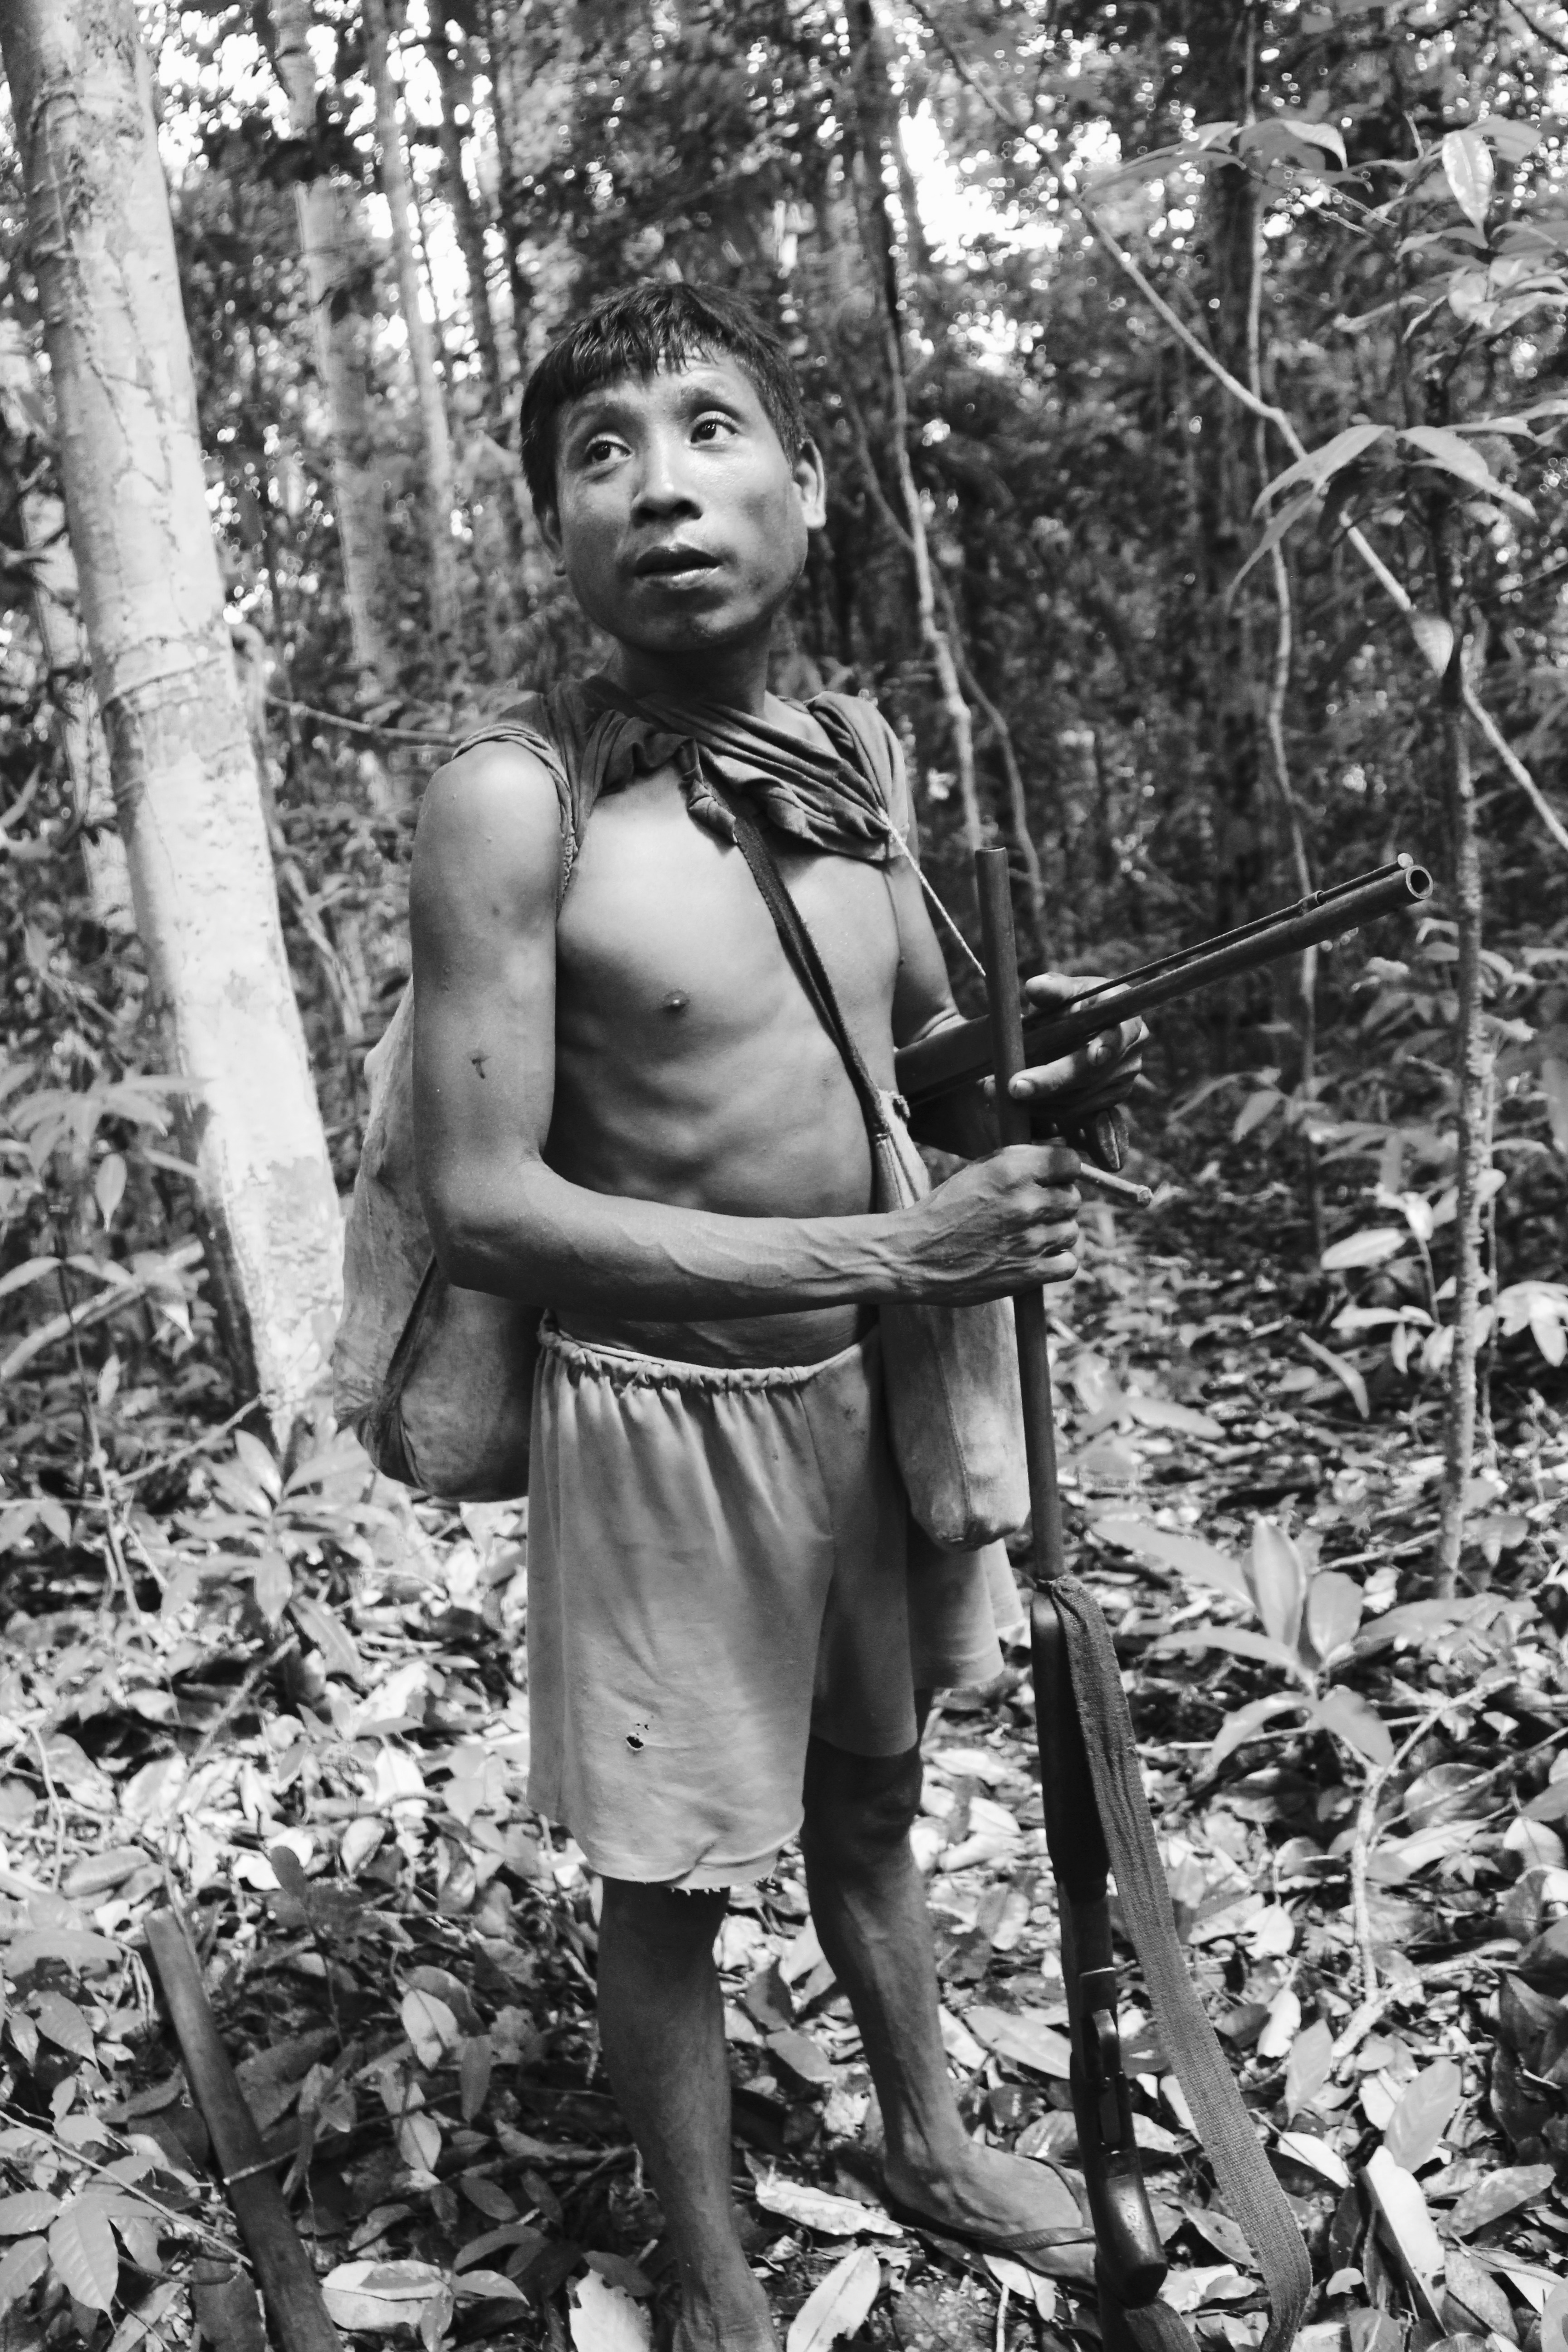
\includegraphics[width=87mm]{./imgs/IMG_1553}
%\caption{Maihuxa’a durante um dia de caminhada, ajudando seu irmão a carregar uma espingarda (acampamento de caça, aldeia Awá, 2013).}
%\end{figure}

\section{\textit{waria}}

\noindent{}Os capelães são animais extraordinários. Ao menos aqueles que vivem nas
matas do Pindaré, Caru e Turiaçu. \textit{Waria}, é como os Guajá chamam
esses animais que eles caçam, criam, cuidam, comem, enfim, pelos quais
se interessam inteiramente. É no ciclo da lua cheia, sobretudo nos fins
de tarde, que o rugido do capelão pode ser ouvido por toda a floresta,
tão alto quanto as cigarras que cantam nos meses quentes. Os
bugios,\footnote{Os primatas do tipo bugio compreendem diversas espécies
  do gênero \textit{Alouatta}, presentes em todo o Brasil e partes da
  América do Sul. Este animal é popularmente conhecido no Brasil como
  ``guariba'', e em boa parte da Amazônia brasileira como ``capelão''.
  Os bugios encontrados nesta região são do tipo \textit{Alouatta
  belzebul}, específicos da mata atlântica nordestina e da floresta
  amazônica (ver Emmons, 1997, pp.\,137--138).} inclusive, já foram
considerados os animais mais barulhentos do mundo. Seu grito, um dos
mais fortes da Terra, pode ser ouvido em uma área de mais de
16 quilômetros.\footnote{Os capelões, ainda hoje, são os mamíferos ``mais
  barulhentos'' do mundo. Veja a matéria ``World's Loudest Animals --- `Power Saw' Cricket'', disponível no site \textit{National Geographic}.} Diferentemente de outros animais (como
queixadas, caititus, pacas e veados), que são mais precavidos e preferem
andar na escuridão da lua nova, os capelães --- tal como as corujas
\textit{waryta} --- gostam do clarão noturno proporcionado pela ``lua
bonita'', \textit{jahy parahỹ}, que é como as pessoas chamam a lua cheia.
Como veremos aqui, os capelães são animais com muitas capacidades, e a
mais fascinante para os Guajá parece ser o fato de ``cantarem''. Dentre
outros aspectos interessantes, na estação chuvosa as fêmeas cuidam dos
machos, espremem-lhes os vermes (chamados \textit{i'urua}) que brotam no
corpo, praticam cuidados dignos de parentes afetuosos; os capelães,
inclusive, são capazes de imitar o som de outros animais para ludibriar
e viver em segurança --- me disseram alguns caçadores. Cada bando desses
primatas gera uma história para ser contada --- depois de os abater, as
pessoas, vendo os corpos no chão, adoram traçar genealogias, apontam
quem era casado com quem, cunhados que não se gostavam, filhos que
estavam crescendo, machos que disputavam fêmeas, e toda a sorte de
conexões genealógicas, tal como primatólogos interessados no
comportamento animal. Certa vez em um acampamento de inverno, ao
voltarmos para casa após uma longa caçada em que dezenas de capelães
foram abatidos --- e as crianças estavam felizes, as mulheres, aliviadas,
dada a fartura de comida e o grande número de provisões que
conseguiríamos moquear para levar de volta para os amigos e parentes que
tinham ficado na aldeia ---, percebi que um dos machos do bando estava com
os lábios superiores destroçados. Hajkaramykỹa era meu anfitrião nesse
acampamento, junto com seu cunhado Takamỹxa'a. Enquanto nos
regozijávamos com a grande quantidade de carne que eles haviam acumulado
na caçada, comentei que um dos capelães havia sido flechado na boca.
Meus anfitriões, discordando, me explicaram que aquele ferimento era
oriundo de um ataque de algum ``parente distante'', \textit{hapihianỹ}, de
algum bando rival. \textit{Hapihiana xu'u}, ``seu parente o mordeu'',
disse Hajkaramykỹa, explicando que era muito comum, após caçarem,
encontrar capelães mutilados pois, eles mesmos, são animais ``bravos'', 
\textit{imahy}, e brigam muito entre si.

Pequenos episódios marcam essa grandiosa relação que os Guajá
desenvolveram com os capelães, e muitas vezes os animais levam a melhor.
Em determinada ocasião, vi uma fêmea carregando seu filhote às costas e,
num ato de desespero, tal como uma heroína, conseguiu escapar das
flechas e tiros pulando do alto da copa de uma árvore alta para outra
mais baixa, a uma altura de quase 10 metros de diferença. A fêmea, mesmo
ferida durante a queda, conseguiu sobreviver e levar seu filhote em
segurança para longe dos ataques humanos. Outra vez, um caçador ficou
doente pois, na volta para casa, após ter abatido alguns capelães, foi
picado por uma formiga tocandira (\textit{Paraponera clavata}), chamada
\textit{takãja} que, como sabem os Guajá, é um ser de criação dos
capelães. A picada dessa formiga --- cuja dor é indescritível --- foi
encarada como um ataque do \textit{ha'aera}, ``vinganças-espectros'', do bando
de bugios mortos. Da mesma forma que, em outra vez, um jovem tomou um
``coice'' da espingarda ao disparar um tiro contra um bando de capelães
e feriu a própria testa. Mais um ``azar'', \textit{panemuhũ}, desses que
aparecem em confrontações de caçada, em que a morte e a dor dão a tônica
desta tensa relação, cujas presas quase sempre indefesas conseguem, por
recursos fantásticos e ao menos algumas vezes, atacar ou se desvencilhar
dos agressores humanos.

O interesse pelos capelães, ou guaribas, não passou desapercebido por outros
pesquisadores que estiveram nas aldeias. Tanto Louis Forline quanto
Loretta Cormier, cada um a seu modo, também atestam isso. O lugar
diferenciado ocupado pelos macacos na vida das pessoas Guajá foi
discutido por Cormier, sobretudo no que se refere a sua adoção como
animais de criação (\textit{pets}, nas palavras da autora); à importância
deles no universo feminino; e ao papel especial que desempenham, se
comparados a outros animais de criação (2003, p.\,113). Cormier lembra
que, embora não tenham um termo lexical para os macacos, os Guajá
utilizam o termo em português \textit{macaco}, para se referir a espécies
de primatas em geral. Além desse, eles também classificam o jupará, 
\textit{hajpaxĩa}, como ``macaco'', devido a sua cauda preênsil, embora
estes últimos, ao contrário dos \textit{macacos}, sejam indomesticáveis
(Cormier, \textit{op.\,cit}., p.\,93).\footnote{Só para termos uma ideia, se
  referiam ao jupará, \textit{hajpaxia}, em português, como
  ``macaco-brabo'', um animal desprezado e que --- nas histórias de assustar
  que contam à noite para as crianças --- seria capaz de raptar e levar as
  crianças com ele.} Na aldeia Juriti, o mesmo ocorria com as
diferentes espécies de primatas, todas também referidas em português por
\textit{macacos}, principalmente aqueles três que as pessoas caçam
sistematicamente para comer (macaco-prego; cairara e cuxiú), à exceção
do guariba, ou capelão, que não seria um \textit{macaco} propriamente, tal
como os Guajá classificam o conjunto dessa espécie. E o guariba, em vez
de \textit{macaco}, é chamado em português por capelão, tal como os não
indígenas da região se referem a esses animais. O macaco-da-noite,
\textit{aparikya}, pode ser chamado de \textit{macaco brabo}, em português,
enquanto que o sagui, \textit{atamari'ia}, seria o \textit{macaquinho} ou,
quase sempre, \textit{atamari'ia}. Nem o \textit{atamari'ia} nem o
\textit{aparikya} são consumidos e, talvez por isso, sejam chamados
\textit{macaquinhos} e \textit{macacos brabos}, respectivamente, em vez de
\textit{macacos}. Há ainda o macaco mão-de-ouro (ou macaco-de-cheiro),
cuja incidência na região do rio Caru (aldeia Juriti) é pequena, mas que
são muito caçados nas aldeias do Pindaré (aldeias Awá e Tiracambu) e que
também, ao serem relacionados em português, são pensados como
\textit{macacos}.

Cormier já alertara que os Guajá consideram os capelães macacos
diferenciados --- já que encontram similaridades entre as duas espécies
(humanos e capelães) --- e consubstanciais aos humanos, nas palavras da
autora \textit{harapiháry}, ``consanguíneos'', ou \textit{harypiana-te},
``afins'', ``verdadeiros'' ou ``próximos''. Segundo a autora, isto seria atestado
pela mitologia, uma vez que os capelães são ex-humanos transformados em
macacos por \textit{Maíra}; e pelo hábito dos capelães de ``cantar'',
referindo-se à vocalização produzida pelos bandos de animais e que pode
ser ouvida por uma extensa faixa territorial, Cormier observa que os
capelães gastam de 3,4 a 34,6\% de seu tempo vocalizando.\footnote{Ver Cormier,
\textit{op.\,cit}., pp.\,93 e 163.}

Os macacos, em geral, também podem ser chamados \textit{ka'ia}, e a
primatologia guajá faz uma distinção categórica entre os \textit{ka'ia},
``macacos'' e \textit{waria}, só ``capelães'' Macacos são os que eu citei
(cuxiú; cairara; macaco-prego, sagui, macaco-da-noite e
macaco-mão-de-ouro, ou macaco-de-cheiro), e nesse grupo não estão os
capelães. O que os Guajá defendem é que ``capelão é capelão'' e ``macaco
é macaco''. Embora \textit{ka'ia} seja o termo específico para o
macaco-prego, incidentalmente pode ser utilizado também como uma espécie
de ``definidor de espécie''. Além da proximidade mitológica e musical,
outras diferenças que envolveriam temperamento e hábitos são utilizadas
para distinguir \textit{macacos}, de um lado, e capelães
(guaribas, bugios), de outro, em que os primeiros seriam culturalmente
superiores aos outros, de uma forma geral. Os capelães encarnam muitos
valores morais que são levados em conta nas caçadas.\footnote{Tal como
  Willerslev aponta para ursos, renas e alces caçados pelos Yukaghir
  (2007, p.\,75).}

Vejamos abaixo algumas comparações.

\begin{enumerate}
\item A distinção inicial é a mesma colocada por Cormier (2003, p.\,93). Os
capelães ``sabem cantar'', \textit{kwa} \textit{janaha}, tal como os humanos.
Quando íamos caçar, muitas foram as vezes que me pediram para levar meu
gravador para gravar --- \textit{pyhy}, ``pegar'' --- o ``canto'' dos capelães, pois
queriam ouvir à noite e mostrar para seus filhos que ficavam em casa e
não iam floresta

\item Se comparados aos capelães, os \textit{macacos} são muito bagunceiros
na floresta. Andam noite e dia fazendo balbúrdia e derrubando todos os
frutos que encontram. Ao contrário, os capelães dormem à noite, andam de
forma mais silenciosa, não são ávidos por comida como os \textit{macacos}
e ``não mexem em tudo''. Seguir os rastros de \textit{macacos} é mais fácil
do que de capelães, pois é só acompanhar o estrago e a bagunça que fazem
pelo caminho, pois jogam folhas e frutos no chão

\item Nos dias chuvosos, enquanto os capelães preferem ficar protegidos
nas árvores, onde tomem menos chuva, os \textit{macacos} podem sair
desembestados, de galho em galho, sem qualquer preocupação com a chuva

\item Mesmo na vida aldeã, como já observei, os Guajá da aldeia Juriti
defendem que a dieta dos capelães deve ser quase que exclusivamente a
mesma que experimentam na floresta, com frutos de maçaranduba, goiabão,
tatajuba, bacaba, copaíba, dentre outros; ao passo que os \textit{macacos}
podem se alimentar com uma dieta mais humanizada (arroz, farinha,
carnes etc.). Embora na prática os capelães também possam comer arroz e
farinha, eles são ditos mais sensíveis à dieta humanizada

\item Cheiros como os de repelente, óleo e gasolina fazem mal à saúde dos
capelães e podem, inclusive, matá-los, enquanto não prejudicam a saúde
dos \textit{macacos}. Quando eu usava repelente, se algum macaquinho vinha
para meu colo não havia problema; porém se algum guaribinha se
aproximava de mim, eles o retiravam dizendo que o odor maléfico do
repelente poderia matá-lo

\item Os filhotes de capelão (além dos macacos cuxiús) são sensíveis a
fotografias. Apesar de não haver impeditivo para fotografar os pequenos
animais de criação que vivem nas aldeias, as pessoas desaconselham
fotografar os capelães e cuxiús de estimação

\item Outro ponto é que os capelães temem a espécie humana mais do que os
\textit{macacos}
\end{enumerate}

De uma forma geral, diferentemente dos capelães os \textit{macacos} são
``salientes'', disse-me em português, certa vez, um homem. Pira'ima'ã
relatou-me que sua mulher criava um capelão, e se ele chegasse perto do
animal vestindo uma blusa, o capelão não mais o reconhecia e se encolhia
de medo. Disse ainda que os capelães preferem os Guajá sem camisa, de
preferência nus, como andavam antes do contato. Os capelães têm medo de
quase tudo o que vem dos \textit{karaia} (brancos); enquanto que, para os
\textit{macacos}, nada disso é problema. Se o contato com os \textit{karaia}
foi, em muitos aspectos, ruim para os Guajá, para os capelães, mesmo os
domesticados, foi pior --- seriam eles, dentre todos os seres, os mais
difíceis de se adaptar à nova (e por vezes infeliz) realidade da vida
pós-contato. O fato é que os Guajá da aldeia Juriti consideram os
capelães uma espécie \textit{única}, diferente de \textit{macacos}.

Essa distinção é muito presente para os Guajá, por não fazerem
diferenciações intraespecíficas tão categóricas na classe dos
\textit{macacos} como fazem entre estes e os capelães. Podem, às vezes,
dizer que os macacos-pregos, \textit{ka'ia}, são mais nervosos ou
bagunceiros; que os cuxiús, \textit{kitxjú}, ou que os \textit{saguis},
\textit{atamari'ia}, são mais infantis e dengosos; ou que os macacos-da-noite
são desconfiados; mas nada que os exclua de sua condição de \textit{ka'ia}
ou \textit{macacos}, bem diferente dos capelães, vistos pelos Guajá como
essa espécie \textit{única}. E se a mitologia explica em parte a
proximidade entre humanos e capelães, ela não explicaria totalmente,
pois, dizem os Guajá, o macaco-prego, cairara e cuxiú, também são
humanos transformados; e nem por isso têm o aspecto especial que os
capelães apresentam.

Vejamos finalmente o assunto que (junto com o canto) mais interessa aos
Guajá: a caça de capelães.

\section{\textit{wari papopo}}

\paragraph{1.}

Em sua etnografia, Cormier observa que, atualmente, do total de proteína
ingerida pelos Guajá, três alimentos despontam como os mais consumidos:
\begin{enumerate}
	\item Os capelães caçados na estação úmida
	\item Os peixes, durante a seca
\item E os queixadas, cuja caça é estável nas estações secas e úmidas\footnote{Cormier, 2003, p.\,40.}
\end{enumerate}

Segundo Cormier (\textit{op.\,cit.}) e Forline (1997) --- que
conseguiram mensurar as quantidades absolutas de alimentos ingeridos
durante todo o período de um ano --- a caça aos capelães é mais elevada ao
final da estação chuvosa e início da seca. Este aumento está associado,
também, ao aumento dos períodos de \textit{trekking} consequentes ao final
das chuvas. De acordo com a autora, uma família pode gastar até cinco
vezes mais tempo em \textit{trekking}, no final da estação chuvosa, do que
no início da estação seca, quando a oferta de peixes é maior e as
pessoas tendem a se sedentarizar, consumindo mais peixes e ficando menos
tempo em períodos de \textit{trekking}. Já iniciada a estação chuvosa, a
partir dos mês de março inicia-se o ciclo conhecido como ``capelão gordo'', 
\textit{wari} \textit{ikira}, como já apresentei no capítulo 2, uma vez
que a estação chuvosa fornece a maior parte dos frutos consumidos pelos
capelães durante o ano.

Se observarmos a caça, os capelães são para os Guajá animais de um
realismo fantástico, e toda a técnica de caça aos primatas é dita ser
tributária do conhecimento que detêm da caça aos capelães. Os Guajá
caçam macacos como caçam capelães, e não o contrário. A flecha para
caças menores, \textit{wy'ya}, como vimos, são feitas especialmente para
matar capelães, e não ``pequenos animais'', mesmo que elas sejam
utilizadas fundamentalmente para caçar todos os animais pequenos.
Durante uma caçada, os capelães são mais ``inteligentes'' do que os
\textit{macacos}, pois conhecem, \textit{kwa}, melhores estratégias de
defesa durante os cercos predatórios, dizem os Guajá. Os capelães não
fogem desesperadamente dos caçadores tal como \textit{macacos}, e, muito
embora sejam pegos fugindo, tentam se camuflar o máximo que conseguem.

Os capelães tomam aqui a forma de ``caça preferencial'' --- tal como
argumenta Hugh-Jones para um outro caso (1996). Mais que os
\textit{macacos}, os capelães são os animais nos quais --- ao lado dos
porcos queixadas --- os Guajá depositam o maior interesse e empenham boa
parte de seus esforços de caça. De acordo com Hugh-Jones,\footnote{\textit{Idem}.} são
dois os fatores que explicariam a predileção pela caça de aves e macacos
em diversos grupos amazônicos: 

\begin{enumerate}
\item Tais animais arborícolas são
encontrados, sendo por isso fáceis de matar (um fator
ecológico-estatístico)
\item Assemelham-se bastante --- embora não muito
--- com aqueles que os comem, devido a seu aspecto sociogregário (fator
moral)\footnote{\textit{Idem}.}
\end{enumerate}

Esses animais seriam diferentes da anta, que anda sozinha
(e não é comida por alguns povos); dos porcos, que são difíceis de
matar; dos peixes, que são somente comida; e da onça, que é predadora.
No caso Guajá, como vemos, a especificidade dos capelães --- como animais
altamente sociais --- e a predileção dos humanos por sua carne parecem ---
corroborando o argumento de Hugh-Jones --- estar de alguma forma
conectadas.

A técnica de caça aos capelães envolve cerco e intimidação, e os Guajá a
denominam \textit{wari} \textit{papopo}, ``espantar o capelão''. Após ser
rastreado e perceber a proximidade do perigo, o bando de animais tende a
se esconder nas partes elevadas da copa de uma árvore ou entre os ramos
de difícil acesso. O cerco dos caçadores consiste em fazer com que esses
escondidos, \textit{imĩ}, fujam de seus abrigos e corram, para que sejam
abatidos na fuga. Desta forma, um homem sobe, \textit{iipii}, na árvore,
onde supostamente se encontram os capelães, enquanto outros sobem em
árvores ao redor, em um raio de 20 a 30 metros. Se a caçada for
coletiva, como muitas vezes é, as mulheres com suas crianças de colo e
algumas crianças maiores permanecem no solo.

Dentre as diversas habilidades necessárias para a caça do capelão, a
primeira que deve ser desenvolvida é subir em árvores --- \textit{ira}
\textit{iipii}, ``subir no pau''. Como todos sabem, macacos (e o capelão
ainda mais, devido a sua constituição física, dotado de uma longa e
forte cauda de pelos curtos), após abatidos, muitas vezes permanecem
presos, enganchados nos galhos no alto das árvores com o auxílio da
cauda, e simplesmente não caem no solo. Os homens, com sua técnica
apurada para subir em qualquer tipo de árvore, sempre alcançam as presas
mortas, por mais presas que se encontrem. Até o contato, subiam usando
uma corda trançada que confeccionavam com folhas de açaí, chamada
\textit{pina'ajna}. Esse instrumento é hoje feito com pedaços de corda que
conseguem ou à moda antiga, a depender da matéria-prima à disposição. De
forma circular, as cordas são encaixadas nos pés dando o suporte
necessário para a subida. Tal recurso é indispensável para a caça de
macacos e capelães (além de outros animais como quatis, ouriços, ou
porcos-espinhos, e diversas aves). As mulheres não sobem em árvores; já
os homens aprendem a técnica ainda na infância, treinando em pequenos
troncos como brincadeira.

Lembro-me de diversas caçadas de capelão, algumas com poucas pessoas,
outras com dezenas. Uma das primeiras vezes em que os acompanhei em uma
caçada dessas foi ainda no meu primeiro período de campo (abril-julho de
2007), justamente no início da estiagem da estação chuvosa, final do mês
de maio. Saímos em um grupo grande, cinco homens, três ou quatro
mulheres e algumas crianças. Takya, um homem velho, havia encontrado
indícios --- \textit{ipopora},``rastros'' --- fezes, urina e pelos no chão e na
vegetação, como já mencionei, de que havia um grupo de capelães em um
ponto distante da mata. Deixamos a aldeia por volta de seis horas e meia da manhã e
andamos por cerca de duas horas, até chegarmos ao ponto. Debaixo da
árvore, não se percebia qualquer sinal da presença de capelães. Enquanto
descansávamos e os homens preparavam suas flechas e espingardas para
iniciarem a caçada, foram chegando mais dois ou três homens que saíram
de casa um pouco depois e que sabiam exatamente em que local estaríamos.
Enquanto mordia e torcia suas flechas, a fim de se certificar se eram os
projéteis adequados para subir, \textit{ipi}, com ele na árvore, Takya
cantarolava (bem baixinho, quase gemendo) o tema musical de
\textit{Juxa'a}, ``gente espinho-da-palmeira-marajá'', um \textit{karawara}
caçador de capelães, como se isso fizesse parte de seu processo
preparatório --- caça e música estão intimamente articulados na vida Guajá,
como veremos no próximo capítulo. A canção insinua, de forma
sussurrada, que os capelães serão mortos bem rápido e que quem está ali
embaixo são grandes caçadores e comedores de capelão, tal como a gente
\textit{Juxa'a}. De acordo com meus interlocutores, isso faz com que os
animais tremam de medo, \textit{iriri}. Todos conversam alto. As mulheres
ficam assobiando um ponto único, repetitivo, e pedem para que eu faça o
mesmo. Os assobios, chamados \textit{opia}, são emitidos para que os
capelães se assustem com a presença humana. Explicam-me que é importante
que os capelães saibam que os homens estão ali embaixo, pois assim ficam
com medo, pensam tratar-se de ``madeireiros'' ou qualquer outro tipo de
ser que lhes fará muito mal. Neste caso, isso é bom para os Guajá. Aos
poucos, os homens --- portando uma espingarda ou seu arco e flechas --- se
espalham em outras grandes árvores situadas estrategicamente em volta da
árvore dos animais. Enquanto eles avançam silenciosamente pelas árvores
--- \textit{ipi} \textit{wate}, ``subir para o alto'' ---, tomando cuidado para que
os capelães não atentem para suas ações, Takya sobe o mais próximo que
consegue da copa da árvore onde os animais se escondem.

Uma vez lá em cima, observa, mexe nas folhas e tenta encontrar algum
vestígio ou esconderijo do camuflado grupo de bugios. Quando,
finalmente, se certifica de que estão ali, inicia uma fala muito
específica. No cerco que se inicia, ganha vida um processo comunicativo
em que o animal é ameaçado, escorraçado de seu abrigo de folhas. Muitos
gritos são dados, principalmente por quem está lá em cima, enquanto quem
permanece no solo ajuda com berros e assobios. Com palavras soltas e
gemidos idênticos ao dos capelães, incitando o bando a correr dali,
Takya grita:

\begin{quote}%\parindent=0em
Corra capelão \textit{rrrrrr, ah ah aaah}\\
Corra capelão\\
\textit{Rrrrrr, ah ah}\\
Corra, \textit{ah ah}\\
Corra mesmo para fora daí\\
\textit{Rrrrrr}, ah ah\\
Saia realmente correndo\\
Dorra capelão, \textit{rrrrrr}, \textit{ah ah aaah}.\footnote{Representei o rugido gutural,
  semelhante ao do guariba, pela sequência de letras \textit{r}, e os gritos
  graves por \textit{ah}.} %No original: ``Awyhy wari, \textit{rrrrrr}, ah ah, aaah / Awyhy wari / Rrrrrr, ah ah / Awyhy, ah ah / Awyhy tete kapo / Rrrrrr, ah ah / Awyhy tete kapo / Awyhy wari, rrrrrr, ah ah aaah''.}
\end{quote}

Trata-se de uma impressionante forma de conexão entre caçadores e
presas. E os capelães também começam a roncar seu som característico, a
ponto de não sabermos qual é a voz humana e qual é o som do animal. A
fala é pontuada por sons idênticos ao dos capelães e proferida até que
surta algum efeito: que eles fujam em direção às outras copas de árvores
onde encontrarão a morte pelas mãos de outros caçadores que os estarão
esperando.

%\textbf{Foto caçadores olhando pro alto}
%\begin{figure}[!ht]
%\centering
%  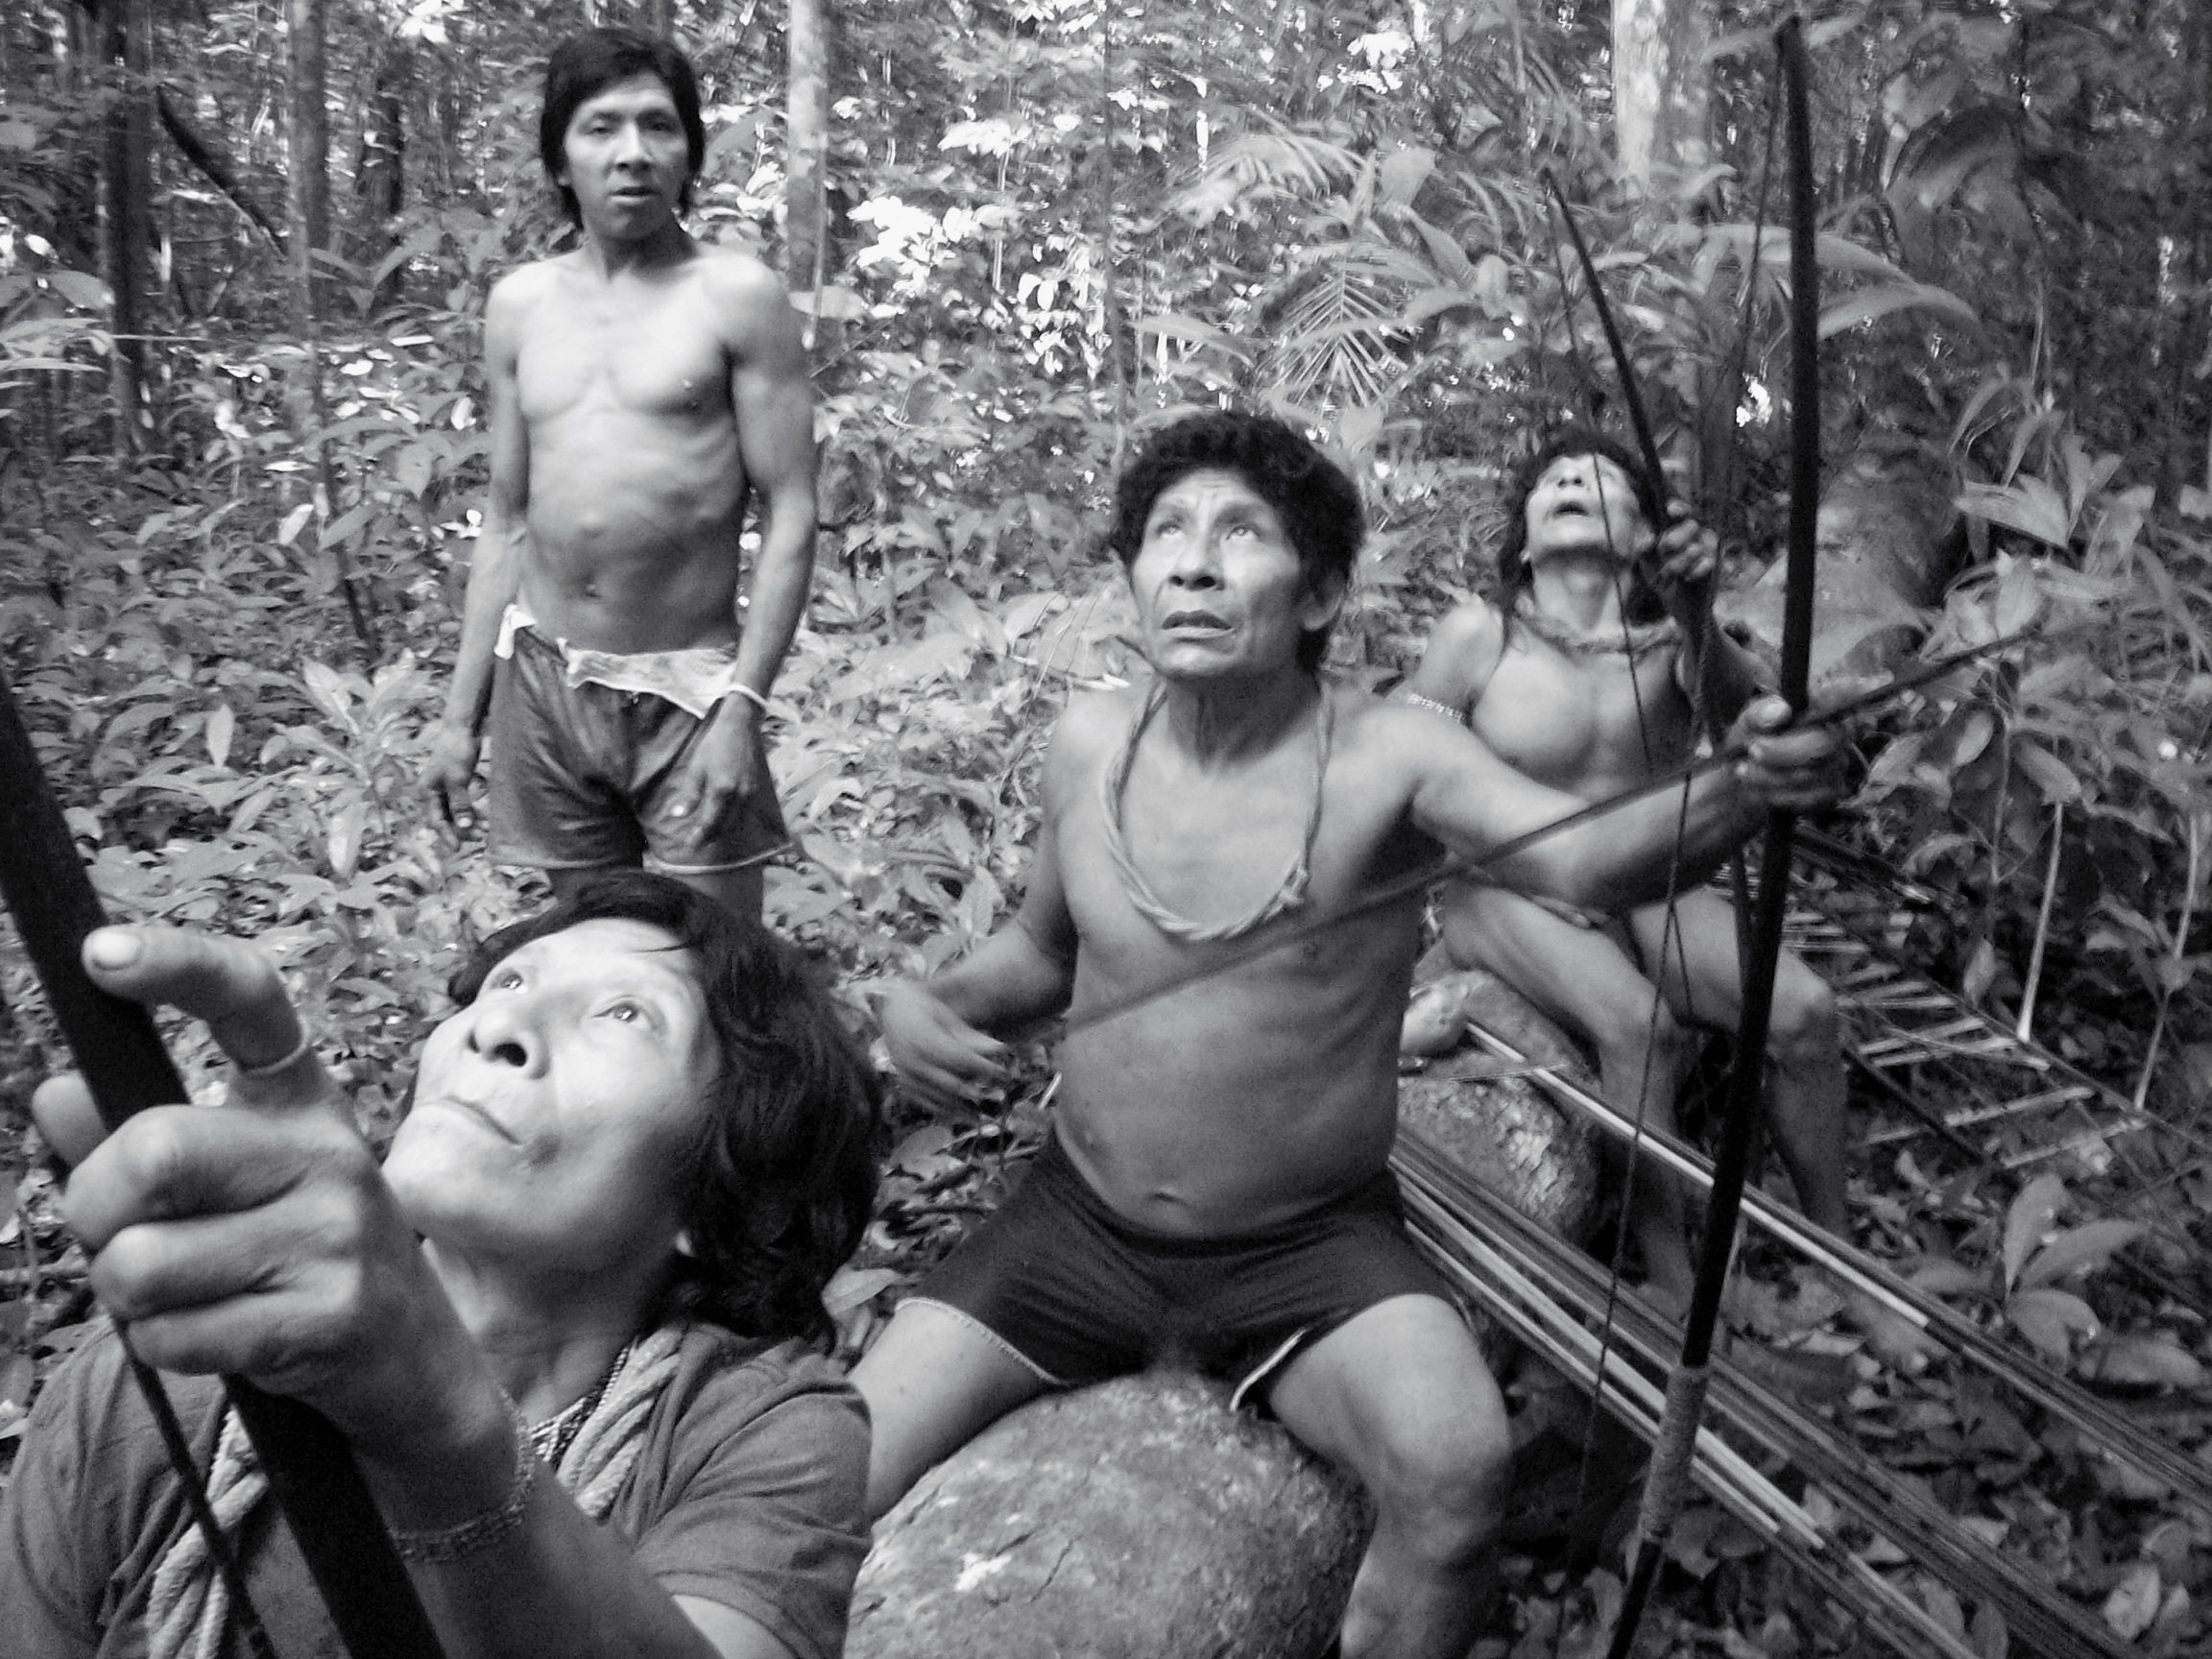
\includegraphics[width=\textwidth]{./imgs/100_5208}
%\caption{Enquanto Uriximatỹa olha para a câmera, Kamará, Takya e Pirama’a observam a copa de uma árvore a procura de macacos (aldeia Juriti, 2007).}
%\end{figure}

Na subida de uma árvore, é importante para quem for espantar os capelães
estar preparado para o inesperado, pois os animais podem correr antes
mesmo de o homem chegar; ou podem permanecer camuflados durante horas,
entre as folhas mais altas da copa, onde o caçador não conseguirá
alcançá-lo, pois corre o risco mesmo de cair de uma altura de até 30
metros. Por meio do silêncio e da camuflagem, que lhes fornece alguma
segurança, os animais, muitas vezes, conseguem fazer com que os homens
duvidem de que estejam lá, como muitas vezes ocorreu. Nessas horas, os
capelães ficavam tão quietos que todos tinham dúvida se havia ou não
animais escondidos. O processo pode durar muitas horas, e os animais
podem, sim, vencer o caçador pelo cansaço. Nesse dia, especificamente,
Takya passou cerca de 20 minutos ``desafiando'' os animais, que em dado
momento se apavoraram com as palavras e fugiram. No momento imediato à
fuga, escutei muitos tiros, misturados a gritos, zunidos de flecha e
rugidos desafiadores. Após alguns segundos, os animais começaram a cair.
Alguns morrem quando são alvejados, outros morrem na queda, e há aqueles
que caem convulsionando, sangrando pela boca e emitindo sinistros
rugidos de desespero. A estes últimos são reservadas pauladas na cabeça
e no resto do corpo, dadas por crianças ou mulheres que cheguem ao
local. Um forte cheiro de urina empesteia o ar, como o cheiro de um
zoológico, pois, como tantos outros animais, os capelães também urinam
na hora da morte.

Neste bando havia sete capelães, sendo que cinco, contando um filhote
não muito pequeno e portanto \textit{imprestável} para criação, foram abatidos. 
Enquanto Takya gritava com os animais no alto
da árvore, as mulheres em solo puxavam longos cipós que caíam até o
chão, para chacoalhar a folhagem da árvore onde estavam escondidos os
animais (muitas vezes, elas obtêm bons resultados com essa operação).
Mulheres mais velhas, como presenciei em uma caçada na aldeia Tiracambu,
podem, do solo, ``espantar os capelães'' proferindo as mesmas palavras que
os homens, e auxiliam quem estiver no alto, \textit{wate}, batendo palmas
e assobiando. Desconfio que o verbo \textit{papopo} tenha o nome \textit{po}
``mão'' incorporado, atestando esses bateres de palma. Depois da caçada,
todos se sentam para limpar suas espingardas, arcos e flechas; os mais
jovens verificam os cartuchos, enquanto os velhos reparam suas flechas
com a mesma preocupação que os jovens preparam novas cargas de munição.
Neste dia, especificamente, Muturuhũ matou dois capelães com suas
flechas; Wirahoa matou uma fêmea e seu filhote com sua espingarda; e o
à época jovem Kaawi'ia, também com sua espingarda, matou um macho.
Kamara se cortou bastante nos galhos, na descida de uma árvore. Ao
final, todos avaliaram seus ferimentos e esperaram o suor secar, com uma
conversa muito animada.

O \textit{wari} \textit{papopo}, ``espantar o capelão'', é uma técnica
bastante eficiente e compõe o aparato de caça Guajá. Ainda assim, muitos
animais conseguem furar o cerco montado pelos humanos, seja porque o
caçador errou seu tiro --- \textit{ajapi jawy}, literalmente ``errei o tiro'' ---, seja
porque o animal conseguiu fugir por um ponto cego, onde não havia
caçadores à espreita. Caso um capelão fure o meticuloso cerco de caça
(como ocorre com frequência), todos os que estão envolvidos na ação se
mobilizam ainda mais: as crianças correm, as mulheres gritam \textit{eles estão
aqui, não os deixem fugir!}, os cachorros latem e os homens, sempre
silenciosos e controlados, descem das árvores e correm em direção às
outras, para onde fugiram os sobreviventes. Mais um pouco, e podemos
ouvir tiros e mais barulhos secos de corpos caindo de alturas de 15 a 20
metros sobre o tapete de folhas que compõe a floresta.

\paragraph{2.}

Como estamos vendo, trata-se de uma emboscada aérea. Os animais devem
ser surpreendidos para que não possam escapar. Em seguida, devem ser
espantados para que, ao fugir, literalmente se atirem contra os
caçadores. Por isso, tais emboscadas são bem-sucedidas se realizadas nas
primeiras horas do dia, quando os capelães ainda estão dormindo. Nenhum
outro animal de caça --- \textit{ma'amiara}, ``caça'', ``presa'', ``bicho'' --- 
tem essa prerrogativa como necessária, a não ser os capelães. Se os homens os
rastreiam ainda pela manhã, a caçada se dá imediatamente. Porém, se
ocorre de encontrarem seus vestígios no final da tarde, sabem que se
instalarão em uma árvore para \textit{cantar} e dormir, pois, diferentemente
dos macacos, os capelães não saem à noite para caçar, \textit{wata}, como
``doidos'', \textit{waky}.

Ao identificar a árvore onde os bugios se instalaram, o homem que a
achou volta para a aldeia --- ou acampamento --- onde estão seus
companheiros e os chama para, no dia seguinte, os abater. Este indivíduo
quase sempre poderá receber uma grande parte do todo abatido, por ter
sido ele quem descobriu os animais. Ele é quem ``puxa'', \textit{myty}, a
caçada, o \textit{tamỹ}, que toma a frente da empreitada e para quem,
muitas vezes, um homem, por algum tipo de serviço como um \textit{serviço da
noiva}, estará caçando. Muitas vezes, os homens --- aparentados
diretamente ou não --- podem ajudar um caçador que tenha encontrado um
grupo de capelães sem que recebam qualquer animal em troca. Esse
propositor da caça é o \textit{tamỹ}, tal como já vimos aqui.

O mais impressionante da caça aos capelães e macacos em geral é que
estes se locomovem pelas copas das árvores e, ainda assim, os humanos
conseguem cercá-los e até persegui-los pelo alto. Boa parte do sucesso
dessa caçada se deve às estratégias de emboscada aérea e ao domínio de
subir em árvores e cipós, independentemente do grau de dificuldade que
essas atividades impliquem. Os Guajá, por exemplo, nunca se conformariam
em deixar um primata enganchado entre os galhos após o abate, por mais
difícil que seja sua captura --- como na cena descrita por Descola em que
um Ashuar, conformado, deixa para trás um macaco-barrigudo preso no alto
da árvore \textit{para os urubus} (Descola, 2006, p.\,155). Caso fiquem
enganchados entre os galhos com seus rabos e membros, como é comum, e se
a árvore for inacessível, sobem em outra próxima e tentam, pelas copas,
chegar até eles. Cortam varas com até cinco metros para alcançar o corpo
do animal enganchado, como se este desafiasse o caçador ainda depois de
morto. Pude presenciar algumas situações em que pensava ser impossível
que pudessem recuperar o cadáver resistente de um macaco ou capelão. E
lá estava o caçador, surpreendendo-me, lançando galhos, subindo em
outras árvores, pendurando-se em cipós. Tudo isso para que os primatas
fossem para o moquém e não virassem ``comida de urubus'', \textit{uru}
\textit{nimi'ũa}.

Gosto de pensar que a caça em geral, e a caça de macacos em particular,
acaba por produzir uma crítica a noções caras a nós acerca de
\textit{animal} e \textit{espécie}. A caça conecta \textit{pessoas} e
\textit{animais} a partir de relações que ora passarão pela criação, ora
pelo abate, mas que nunca serão concomitantes, tal como ocorre conosco
em casos como a criação de bois e galinhas. Em outras palavras, tal como
sabemos, o que se cria não se mata, o que se mata não foi criado, e isso
pode não ser trivial. Certa feita, um amigo abatera um macaco-prego com
um tiro na parte traseira do crânio. O cérebro do animal ficara exposto,
e mesmo depois de horas após a caçada podíamos ouvir no pátio de nosso
acampamento o bicho moribundo lutando para não morrer. Lembro que aquela
cena me atormentou, acabei pedindo para que alguém terminasse de vez com
o animal para aliviar a si próprio ou a mim de tanto sofrimento. Foi quando
todos que me ouviram desataram a rir, não sem acatar os meus apelos.
Sobre o animal, além de me mencionarem uma ideia que alguns Guajá
defendem e que nunca entendi direito, a de que ``bicho não sente dor'',\footnote{ \textit{Nikaj hahyha}, ``não sente dor''.} o outro comentário que me
fizeram, entre muitas risadas, era o fato de aquele macaco resistente
ser parecido com os \textit{brancos} e ser difícil de matar --- \textit{de morrer},
para ser mais preciso. Tal maneira de pensar macacos como animais de
caça é estranha a mim, pois somos informados pela nossa primatologia,
pelo nosso etno-conhecimento, de uma continuidade lógica e inseparável
entre nós e os primatas, algo que os Guajá não compartilham. Meus amigos
neutralizam isso muito facilmente retirando não só os macacos, mas todos
os animais caçáveis dessa linha de continuidade interespecífica --- do
tipo ocidental \textit{somos todos animais} ---, o que faz tudo mudar. É como
se, para os Guajá, a \textit{caça}, como um modo de interação, em nada
tivesse a ver com a \textit{domesticação} de animais, como outro modo.

A tônica, portanto, não recairá na \textit{espécie} tal como nós
concebemos cachorros como um tipo de animal e jaguatiricas como outro),
mas em distintas formas de relação; ou, podemos pensar, diferentes
afecções. Como se os animais de um tipo (caçados) tivessem pouca relação
com animais do outro tipo (criados), mesmo sendo um da mesma
\textit{espécie} que o outro. A natureza das interações entre humanos e
animais, na caça e na domesticação, são não apenas de universos
diferentes, mas a própria ideia de \textit{animal} pode não ser informada
pela ``animalidade'' de certas espécies em oposição a ``domesticidade''
de outras, mas pela forma com que os Guajá se relacionam com esses
bichos. Por exemplo, tal como outros povos amazônicos, os Guajá não têm
uma palavra para \textit{animal} \textit{genérico},\footnote{Ver p.\,ex. Vander Velden,
2012, p.\,238.} mas guardam uma para animal ``caçável'', 
\textit{ma'amiara}, e outra para animal ``criável'', \textit{hajma}.
Por esta lógica, um macaco-prego na floresta pode vir a ser mais
perigoso do que uma onça doméstica --- e as pessoas lembram todo o tempo o
quanto os macacos-pregos são agressivos e \textit{doidos} ---, não havendo um
\textit{a priori} de agressividade da espécie, embora os Guajá defendam
que, no mato, uma onça {[}quase{]} sempre será mais perigosa que um macaco.

Se essas duas características são indissociáveis, como sabemos da caça
amazônica, no caso Guajá uma se vincula diretamente à outra, em que a
comida e a criação são condicionantes entre si, operando algo como um
\textit{duplo vínculo}, tal a célebre formulação de Gregory Bateson, pela
qual, o que quer que se faça para se desvencilhar, não há como vencer
(1956 {[}2000{]}): para os Guajá criarem precisam matar, para caçarem
precisam cuidar. É comum ver homens que saem para o mato para caçar
dizerem a suas filhas que trarão como regalo um filhote de macaco ou de
cotia, produtos da caçada que farão. Também vemos meninas que desatam a
chorar por não terem um animalzinho de criação serem consoladas por seus
pais e mães que prometem lhe trazer um quando houver uma nova caçada. Os
homens Guajá reclamam que suas crianças choram querendo filhotes de
macaco e cotia para criar. Sendo assim, e como sabemos de tantos povos
amazônicos, na mesma jornada que se produz comida na forma de caça são
capturados os animaizinhos de estimação. Porém, diferentemente de
concluir que a criação desses seres funcionaria como uma compensação
pela morte de seus semelhantes caçados, como outros autores o fizeram,
no que concerne a diferentes animais, comidos e criados, esse fenômeno
parece recolocar a própria ideia de \textit{espécie} como algo dado. Ao
menos sob a perspectiva humana, parece que estamos diante de diferentes
\textit{tipos de animais}, por assim dizer, que aparecem, para os humanos, como efeito de
relações. Não apenas o próprio bicho,
mas o tipo de relação importaria tanto quanto a espécie do animal. É a
\textit{relação}, se assim posso colocar, que parece primária aqui, seja
no tratamento cuidadoso dos animais criados, seja na forma \textit{impiedosa}
que reservam aos animais caçados. Neste caso, a própria noção de
\textit{espécie}, em debate há pelo menos 150 anos
na biologia,\footnote{ Ver Haraway, 2003, p.\,15.} seria subordinada a esse \textit{duplo
vínculo}, não havendo a \textit{espécie} em si, mas \textit{agenciamentos} de
caça e outros de criação. Para esta etnografia, são esses diferentes
modos de relação que interessam, e não os bichos, espécies, gêneros,
ordens ou classes em si.

\section{entre o rastro e o som: a poética da predação}

Os Guajá dificilmente caçam os capelães no final da tarde, hora em que
os animais estão \textit{cantando}. Ao contrário, ao perceber os capelães
cantando, param para ouvi-los, e, pelas vozes, conseguem distinguir
quantos são fêmeas ou machos; adultos ou filhotes. E então traçam planos
para o dia seguinte, quando os perseguirão. Certa tarde, eu andava com
Pira'ima'ã na floresta quando ouvimos um grupo de capelães entoando seu
som característico. Com o que ouviu, ele conseguiu todas as informações
de que necessitava para o dia seguinte: tratava-se de uma fêmea
solitária com dois filhotes em uma copa, enquanto o resto do grupo
estava um pouco mais distante. Ele me explicou que o som emitido pelas
fêmeas é mais delicado do que o do macho, que tem um \textit{canto} grosso. Em
outra situação, ao ouvir sons de capelães comentei com Ajruhua sobre o
canto. Ela me respondeu que eram filhotes e que não estavam cantando,
\textit{jã}, mas sim, chorando, \textit{ja'o}, pois quem cantava eram
apenas os adultos da espécie. Escutar, \textit{nũ}, o som-canto, 
\textit{jã}, dos animais é fundamental para as caçadas, sobretudo de
capelães. Sentenças como \textit{vamos caçar capelães amanhã, pois alguém os
ouviu cantar naquela direção!} ou \textit{vamos sair para escutar os
capelães!}, dentre tantas outras formas, associam o som-canto do capelão
com a busca pelo animal. Em outras palavras: \textit{é preciso saber
escutar os capelães} {[}e demais presas{]} \textit{para poder caçá-los}. Pelo
canto dos capelães, sabe-se a quantidade e a diversidade do bando, tal
como a pegada de um animal terrestre revelará seu peso, idade, sexo e
outras informações relevantes.

Ouvir os capelães pode ser encarado como uma ``estratégia de caça'', mas
sabemos há algum tempo que as ``estratégias'' de povos como os Guajá
(caçadores, por excelência) não se resumem a um jogo de sobrevivência e
forrageio. Suas práticas de produção da vida estão longe de um aspecto
comportamental ilógico, pois não podemos reduzir as atitudes dessas
pessoas a um economicismo que tende a naturalizar (no sentido de colocar
no plano da Natureza) as atividades de caça, coleta, dentre outras
(Ingold, 2000, p.\,58). Os Guajá, por exemplo, param para escutar os
capelães independentemente de caçá-los ou não, pois (como sempre
afirmam) ``gostam'', \textit{maparahy}, do canto deles e sempre que podem
elogiam a capacidade que tais animais detêm de ``cantar bonito'', 
\textit{jã} \textit{paryhỹ}. Para as pessoas da aldeia Juriti, eu sempre
deveria gravar o canto dos capelães com a mesma assiduidade com que
gravava o canto humano e com o mesmo objetivo: levar para São Paulo e
mostrar aos outros brancos como os \textit{awatea}, as ``pessoas'', mas
também os capelães, ``sabem cantar'', \textit{kwa} \textit{janaha}. É claro
que muitos animais conseguem cantar (os pássaros são o maior exemplo
disso), mas os capelães eram os únicos que lhes interessavam gravar.
Foram muitas as vezes em que pudemos ouvir, de muito longe, no final da
tarde, capelães produzindo seus sons característicos. E sempre havia
alguém pedindo para que eu gravasse seus rugidos. Eu, gentilmente,
atendia ao pedido, mas apenas para mostrar que o sons da aldeia
(crianças, galinhas, cachorros) e os sons da floresta (vento nos galhos,
assobios de pássaros e outros animais) se interpunham entre o gravador e
o canto dos capelães, o que não permitia que o canto, que estava longe,
fosse bem registrado.

Sem dúvida, \textit{ouvir} pode ser uma das melhores formas de conhecimento
quando as pessoas vivem na floresta, como é o caso de diversos grupos
amazônicos. Com o campo de visão limitado e a necessidade de não serem
vistos, a espreita e a escuta são formas extremamente adequadas a essa
realidade.\footnote{Como escreve Cabral de Oliveira para os Wajãpi, ``O
  ouvido atento é marca de um bom caçador'' (2012, p.\,97).}

Porém, os Guajá sugerem que a caça em si (como continuaremos vendo)
oferece outras sensações aos humanos. E, por mais contraditório que isso
possa parecer para a nossa tradição de pensamento, que tende a separar
algumas espécies animais para se afeiçoar, enquanto outras são para
consumir,\footnote{Ou, como observa Erikson: ``\textit{nous nous efforçons
  de séparer radicalement le familier et le comestible, alors que les
  Amazoniens sont pour leur part soucieux d'un juste équilibre entre les
  deux}'' (Erikson, 1997, p.\,03).} o fato de as pessoas gostarem da música
dos capelães é o mesmo que os faz gostar de os matar. Criá-los e
caçá-los não são aqui duas formas de relação tão diferentes entre si.
Vejamos melhor esta suposição.

Talvez tenha sido Ingold quem melhor observou que, entre muitos povos
não ocidentais, e em particular os chamados caçadores-coletores, ``a
diferença entre as atividades de caça e coleta, de um lado, e cantar,
narrar estórias e mitos, de outro, não podem ser postas em termos de uma
dicotomia entre material e mental, entre interações ecológicas \textit{na}
natureza e construções culturais \textit{da} natureza'' (Ingold, 2000, p.
57). Para o autor, ``ao contrário, ambos os conjuntos de atividades são,
antes de tudo, maneiras de habitar {[}no mundo{]}, \textit{dwelling}''.\footnote{Para o sentido exato da ideia de
  \textit{dwelling} \textit{perspective} --- um conceito central nas análises
  de Ingold ---, ver Ingold, 2000, pp.\,153--156.} Trata-se de um
``envolvimento poético'' (nas palavras desse autor) que, no caso Guajá,
sugere que caçar não é apenas conhecer (espécies e hábitos animais), mas
se engajar com tais espécies, habitando um mundo em que a caça ganha
elementos da \textit{guerra} e os animais não são coisas destituídas de
\textit{alma} ou personalidade. Hugh-Jones observa que o idioma da guerra é
utilizado por grupos do noroeste amazônico, sobretudo quando se referem
a caçadas coletivas. De acordo com o autor, os queixadas naquela região
encarnam a imagem do inimigo selvagem em ataque. E, ``embora toda caça
coletiva conote de uma maneira ou de outra a guerra, esse efeito é
ampliado de acordo com o número de queixadas'' (1996, p.\,14). No caso
guajá, encontramos também paralelos com essa ideia.

Os Guajá defendem que, ao emboscarem os capelães, os animais
\textit{falam} entre si: ``vamos embora, pois estamos cercados por
inimigos'', \textit{mihua}, e \textit{inimigos}, nesse caso, deve ser
entendido como uma \textit{posição} ocupada pelos humanos, a partir do
ponto de vista dos capelães, para evocar aqui a noção de \textit{ponto de
vista} discutida na etnografia yudjá (Lima, 1995, 1996, 2005). O tipo de
inimigo, \textit{mihua}, variará conforme o narrador da caçada e da
situação. O importante nessa ideia é que os animais apreendem os humanos
enquanto \textit{inimigos}, podendo ser \textit{madeireiros mihua}
(madeireiros-brabos), \textit{karai} \textit{mihua}, ``brancos-brabos'', ou
\textit{awa} \textit{mihua}, ``gente-braba''. Isto é indiferente, pois o efeito
produzido na \textit{mente}\footnote{Refiro-me à ``mente'' a fim de
  explicitar que os guaribas ``pensam'' --- \textit{imarakwa}, ``pensar'', ``imaginar'' --- 
  se tratar realmente de inimigos, tal como os Guajá
  definem.} dos animais é o mesmo. A ideia-imagem de \textit{karaia}, ``brancos'', 
  como sinônimo de inimigo, por exemplo, é recorrente quando
comentam a relação entre a caça --- \textit{ma'a}, ``presa'' --- e caçador
--- \textit{watama'a}, literalmente ``caminhador''. Quando relatam que certo
animal fugiu podem, em tom jocoso, dizer, modificando a voz, ``corram,
corram, os \textit{karaia} estão doidos e estão vindo nos matar, corram'',
e todos caem na gargalhada.

Um termo que entrou definitivamente para o léxico da língua guajá é
\textit{índio}, que pode ser utilizado de diferentes maneiras. Na forma
\textit{positiva}, como sinônimo de \textit{awatea}, ``humanos'', 
o utilizam quando se referem à terra indígena: \textit{essa terra é
nossa, é terra de índio}, ou quando queriam que eu entendesse a quantidade de pessoas
que habitavam o céu, \textit{iwa}, também diziam ter \textit{muitos índios}
(humanos). Porém, por ser uma ideia \textit{importada} e bem maleável, também
pode aparecer como sinônimo de \textit{mihua}, ``inimigo'', e vir ou não
acompanhada do adjetivo \textit{brabo} (``\textit{índio} \textit{brabo}''). Por
isso, durante as caçadas os capelães podem ser ditos \textit{índios};
nesse caso, um sinônimo para ``inimigo'' e/\,ou ``não semelhante''. Uma das
primeiras vezes em que ouvi se referirem desta forma foi durante uma
caçada de capelães {[}que acompanhei{]}, quando os animais se anteciparam
aos caçadores e conseguiram escapar, deixando todos muito tristes. Em
seguida um homem veio falar comigo, ``\textit{índio} \textit{wyhy}'', ``índio
correu'', e os \textit{índios} em questão eram os capelães. Assim, para os
capelães, os Guajá são \textit{madeireiros}, \textit{brancos}, \textit{índios}, ou qualquer outro termo que ocupe a posição de inimigos, que irão
matá-los, por isso fogem com seus filhotes.

Da perspectiva do animal predado, portanto, a caça é uma guerra em quem
os humanos, \textit{awa}, podem matar os animais --- \textit{ma'amiara},
``presa'' ---, e por isso eles enxergam os humanos como inimigos, 
\textit{mihua}. O mesmo encontramos em exemplos paradigmáticos como na
etnografia Araweté na qual ``para os animais, os Araweté são \textit{awĩ},
inimigos --- exceto para a onça, que, ela é que é \textit{awĩ}, e nós seus
\textit{hẽmĩnã}, `presa'. É por isso que se dança sobre a morte de uma
onça como sobre a de um inimigo'' (Viveiros de Castro, 1986, p.\,350).
Entre os Araweté pode ser encontrado algo próximo --- em conteúdo e forma
--- ao caso Guajá da caça aos capelães como uma caça extremamente
sociável. Viveiros de Castro observa:

\begin{quote}
Os queixadas e guaribas, certamente devido a seu costume de viverem em
bandos, são uma fonte rica de metáforas da sociedade para os Araweté, e
sobretudo da relação de guerra entre sociedades. Assim, eles sempre
comparavam a técnica de cerco kayapó com a que eles utilizavam contra as
varas de porcos; e gostavam de arremedar o pânico dos guaribas e porcos
quando atacados pelos caçadores; os bichos gritariam: `\textit{awĩ},
\textit{awĩ}!'. Os jabotis, por sua vez, são comparados a cativos de
guerra, por ficarem presos nas casas até serem mortos e comidos. A
associação entre caça e guerra é clara para os Araweté (como para os
Wayãpi. \textit{Cf}. p.\,Grenand, 1982, p.\,208; 1980, p.\,42).\footnote{Viveiros de Castro, 1986, p.\,209.}
\end{quote}

É importante observar que a caça guajá está baseada na ideia de que boa
parte dos animais enxergam os humanos como inimigos, \textit{mihua}. É
isso que orientará as técnicas, pois os humanos caçam seres que
{[}sabem{]} os percebem como inimigos. Mais do que isso, pois, se em linhas
gerais podemos afirmar, parafraseando Lima, que \textit{aquilo que os humanos
apreendem como caça, os capelães\footnote{A autora se refere a
  \textit{porcos}, e não a capelães.} apreendem como guerra} (1996, p.
34); a perspectiva da guerra não pode ser relegada ao mundo animal,
quando os humanos apenas \textit{caçam} e os animais \textit{combatem}. Os humanos
precisam utilizar um arsenal simbólico-guerreiro para fins
ecológicos-alimentares. \textit{Caçar capelães}, portanto, além de se basear no
ato de ``espantar o capelão'', \textit{wari} \textit{papopo}, é
potencialmente uma atividade de \textit{ha'a waria}, ``enganar o capelão'',
e isso é feito de forma muito consciente, em que os humanos aproveitam o
fato de serem vistos pelos animais como \textit{inimigos}. Podemos pensar
que, se durante uma caçada os humanos são vistos como inimigos, 
\textit{mihua}, aos olhos dos animais, é porque também eles \textit{se
tornam capelães para caçar} e guerrear com outros, agora, ao menos para esse fim estratégico, 
parcialmente \textit{iguais}. Muitas das caçadas
guajá estão baseadas na imitação, gerada por um profundo conhecimento
dos hábitos animais; os homens precisam falar a língua dos capelães
para que eles pensem que se trata de algum tipo de ser próximo --- não importa se um
parente distante, \textit{harapihianã}, ou um inimigo, \textit{mihua}.

Parte da habilidade do caçador é apoiada nessa capacidade de
\textit{mimetismo}, tal o sentido que Willerslev (2007) empresta ao termo. Em
sua etnografia sobre os Yukaghirs, um povo da Sibéria Oriental,\footnote{Os Yukaghirs são caçadores de alces e renas, produtores de pele e detentores de uma técnica apurada para a caça desses animais, que, pelo uso de peles,
gemidos e movimentos, se \textit{transformam} em alce a fim de os caçar.}
Willerslev introduz um problema análogo ao que encontro aqui, porém em
uma paisagem etnográfica muito distante. De acordo com o autor, a caça
de alces Yukaghirs propõe uma equação de difícil resolução, uma vez que,
ao se passar por alces, os homens experimentam uma situação liminar,
pois, se um caçador não é propriamente um alce, ele também \textit{não é
um alce}, ocupando \textit{um estranho lugar entre as identidades humanas e
não humanas} (Willerslev, 2007, p.\,1). Pensando a partir dessa ideia, a
imitação envolvida na cinegética Guajá funciona não como uma forma de
representação que os caçadores descobriram apenas para assustar os
capelães, mas sim como uma forma de relação assimétrica cujo polo é
marcado por um exercício de poder guerreiro, de caçadores sobre essa
espécie, cujo objetivo final é a predação.\footnote{Ver Willerslev, 2007, p.\,11.}
A fala do capelão é vista na boca humana, e se não acontece uma
metamorfose de um no outro, humanos tentam transformar um tipo de
perspectiva que os outros {[}capelães{]} têm sobre eles {[}humanos{]}. A
questão, tal como discutido por Willerslev, é que os caçadores irão
experienciar os animais como pessoas a partir de um ponto de vista
similar, mas não idêntico ao deles {[}animais{]} (2007, pp.\,98--99).

O autor não deixa de mencionar que o fato de um caçador ser como a presa
faz dele, sem dúvida, uma estranha presa, pois --- por mais semelhança que
ele tente estabelecer com o animal a ser caçado (um registro sonoro, no
caso Guajá; ou visual como no caso Yukaghir) --- as diferenças reais entre
caçador e presa continuam sendo incomensuráveis. Por mais que um caçador
guajá queira (embora eles não queiram), nunca se parecerá inteiramente
com um capelão, pois a identificação mimética entre um caçador e sua
presa não é mesmo para ser \textit{total}, porém \textit{parcial}, e é
justamente essa pequena diferença sobre o mundo representado que faz com
que o caçador exerça poder sobre essa presa, pois, ``sem diferença,
imitador e imitado entrariam em colapso, um se tornaria o outro,
tornando qualquer exercício de poder algo impossível'' (Willerslev, 2007,
p.\,11).\footnote{Essa também será a definição de Pendersen para
  \textit{animismo}, formado por identificações análogas, ou parciais, e
  não totais (Pendersen, 2001 \textit{apud} Willerslev, \textit{op.\,cit}., p.\,24)}
Citando-se novamente o etnógrafo siberianista: ``O caçador sabe, ou ao
menos deveria saber, que o alce e ele não são exatamente os mesmos''
(2007, p.\,99). Além disso, tornar-se um outro animal é, como sabemos há
algum tempo, uma das piores catástrofes que se podem abater sobre a
pessoa, tanto ameríndia (Seeger \textit{et al.}, 1979; ver também Viveiros
de Castro, 2002, pp.\,390--391) quanto na Sibéria (Willerslev, 2007,
pp.\,99--100). Trata-se, para a caça de capelães, de uma metamorfose
corporal, porém de risco calculado, pois fica óbvio que os Guajá não
colocam sua relação com os capelães em níveis simétricos. Ora os
capelães são animais de criação, \textit{nima}, ora são comida, 
\textit{hami'ũa}. Antes de comida, caça, \textit{ma'a}. E para que sejam
caçados se tornam inimigos, \textit{mihua}. Serão sempre relações que
envolvem assimetria --- termo mais adequado à paisagem amazônica do que
``poder'', como proposto por Willerslev para a Sibéria. Assim, fazer com
que os capelães pensem ser o caçador um igual, ainda que inimigo
(\textit{like-me-but-not-me}, Willerslev, 2007, pp.\,98--99), é um ponto de
destreza ao mesmo tempo que uma condição da atividade de caça.

Ingold se reporta a uma ``economia cósmica de compartilhamento''
(\textit{cosmic} \textit{economy} \textit{of} \textit{sharing}), em que animais
e plantas mantêm com os humanos uma relação de ``parceria'' --- embora entre
os Guajá estejam ausentes características de ``devoção'' à ``mãe da caça''
ou ao ``espírito do vento'' que propiciam uma boa caçada, como vemos em
caso de caçadores do ártico e subártico, além de em outros casos
amazônicos.\footnote{Ver Ingold, 2000, p.\,48 e Descola, 2005, pp.\,459--496 para
exemplos diversos; e Descola, 2006, p.\,172, pra um caso amazônico.} Para
diversos grupos, observa Ingold, a caça deve ser ``encarada não como uma
manipulação técnica do mundo natural, mas como uma espécie de diálogo
interpessoal, parte integrante de todo o processo da vida social em que
pessoas humanas e animais são constituídos com suas identidades e
propósitos'' (Ingold, 2000, p.\,49). O que encontramos aqui entre os Guajá
é um certo ``padrão amazônico'' para caça, em que elementos de guerra são
reais também para a atividade caçadora --- no sentido de uma ``confrontação
coletiva'', tal como prescreve Descola para os conflitos, sejam de caça
ou de guerra, na Amazônia (1993, p.\,171; 2005, p.\,461), e que no caso
Guajá envolve vingança, resguardo, dentre outros elementos que veremos
aqui.

Além das habilidades e equipamentos necessários, conforme já demonstrado
aqui, toda a caça de capelães e boa parte da lógica da predação animal
Guajá está baseada em induzir a caça ao erro, ``enganar a caça'', 
\textit{ma'amiara} \textit{ha'a}, como afirmam os caçadores. Um bom caçador
é aquele que, a partir das técnicas certas (silêncio, imitação,
rastreamento), faz com que o animal caçado se confunda e cometa erros
que não cometeria em uma situação de ``equilíbrio'' (como na ausência do
caçador, por exemplo). Os Guajá imitam com perfeição grunhidos e
assobios de diversos animais --- muitos dos quais não são caçados ---, e
essas imitações aparecem para ilustrar de forma magnífica as narrativas
noturnas sobre as caçadas, chamadas \textit{mumu'ũha ``narração''}. Tais
imitações, porém, extrapolariam a barreira estética (apesar de seu
realismo e beleza) e são também uma forma de conexão com a presa,
formando algo como uma \textit{poética da predação}. O caçador Guajá é,
nesse caso, uma espécie de influenciador que se disfarça entre as
folhagens e, com assobios e gemidos característicos de cada animal,
consegue confundir a presa, atraindo-a para a morte, quando a faz pensar
tratar-se de um semelhante. Para caçar é necessário que se comuniquem
--- \textit{ma'i} ``falar''; ou \textit{hamakaj} ``chamar'' --- com os animais por
meio desses chamados específicos. Tal comunicação é chamada \textit{ha'ỹ
hanima}, ``chamar o meu animal de criação'', o que acena para uma relação,
ao menos liminar, entre ``animais de caça'' e ``animais de
criação''.\footnote{Ha'ỹ é mais do que ``chamar''. Além de ``imitar'', o
  mesmo verbo é utilizado também com o sentido de
  ``experimentar'', ``tentar'' para quando querem comer uma comida nova ou
  tentar fazer algo que nunca fizeram. Um sentido mais geral para esse
  verbo, que englobe essas noções, pode ser algo do tipo ``fazer
  igual''.} Neste caso, caçadores utilizam recursos miméticos para
ludibriar suas presas, fazendo-as acreditar que, em vez de matadores, os
sons são provenientes de seres de seu universo ``familiar'' (os
\textit{hapihiara}, ``parentes próximos'', diriam os Guajá; ou mesmo os
\textit{jara}, donos de animais de criação). Nesses momentos, as
diferenças entre animais de criação --- \textit{hanima}, ``meu animal de
criação'' --- e de predação --- \textit{hama'a}, ``minha caça'' --- estão suspensas,
visando a melhor estratégia (guerreira) de caça. Uma presa
\textit{ma'amiara}, portanto, pode ser tratada, mesmo que por um
momento, como um animal de criação, em um chamamento suave, um som
confiável, feito para enganá-la. Aquilo que aos ouvidos dos animais é
fala ou canto, \textit{poética} é, por uma inexorável verdade, o
prenúncio da morte, \textit{predação}.

Para o veado, \textit{arapaha}, emulam um gemido anasalado,
``\textit{mẽẽẽ}'', idêntico ao que é produzido por este cervídeo. Assim, o
animal pensa --- \textit{imarakwa}, ``pensar-imaginar'' --- tratar-se de um
outro de sua espécie. Para a cotia, \textit{akwixia}, produzem um som
aspirado, principalmente quando não a encontram ou quando o animal está
em fuga. Ainda conseguem imitar o som de filhotes de cotia, para
ludibriar adultos da espécie e os atrair. Quanto a esta última
possibilidade, reescrevo um depoimento de Wirahoa que me foi concedido
em 2008:

\begin{quote}
Ao encontrar uma cotia prestes a fugir, se a chamo, imitando o som de
um filhote, ela pensará que os ``brancos'' --- \textit{karaia}, nesse caso
sinônimo de ``inimigos'' --- aprisionaram seu filhote. Ao ouvir o meu
chamamento, a cotia bate suas patas no chão em desafio, como se
pensasse, ``o que esses \textit{karaia} estão querendo ao aprisionar o meu
filhote?''. Com isso consigo deixá-la com dúvida, se questionando sobre a
veracidade dos choros que está ouvindo. Enquanto ela está parada,
``pensando'', eu atiro e a mato. Então, ao morrer ela pensa, ``não havia
nenhum filhote aprisionado; foram os \textit{karaia} que me enganaram, só
para comerem minha carne''.
\end{quote}

Este exemplo é interessante também para notarmos que, de acordo com essa
teoria guajá --- que é, de muitas maneiras, perspectivista ---, os caçadores
nunca serão \textit{awatea}, ``gente'', para os animais caçados. Se as presas
pensam, e caso tomem os caçadores por algum tipo de humano, estes
últimos encarnarão justamente os \textit{karaia}, ``não indígenas'',
justamente o tipo de gente que os Guajá, apesar de viverem próximos hoje
em dia, tendem a evitar.

Antes de seguirmos para outro exemplo, lembro que, diferentemente dos
capelães, que roncam, os outros \textit{macacos}\footnote{Macaco-cairara, cuxiú e
macaco-prego, ou \textit{ka'ihua}, \textit{kwixua} e \textit{ka'ia}
respectivamente.} contam não só com gritos estridentes que lhes servem de
proteção, mas também com assobios, com os quais os indivíduos de um
bando se comunicam. Embora a técnica de ``espantar o capelão'' possa ser
utilizada para a caça de macacos em geral --- como presenciei por diversas
vezes, quando os bandos de macacos se escondiam na copa de uma árvore e
os caçadores alcançavam o mesmo sucesso que obtêm com os capelães ---, os
assobios dos outros \textit{macacos} também podem ser imitados pelos
humanos. Enquanto com os capelães a técnica específica é o \textit{papopo}
(espreita e espanto), quando se trata de macacos os caçadores podem
mimetizá-los de outras formas, sobretudo por meio dos ``diálogos''
assobiados que os diversos primatas, como os macacos-pregos, travam.

Na caça aos diversos tipos de macacos, os assobios característicos
emitidos pelos primatas em sua comunicação são reproduzidos por um
caçador a fim de os ludibriar, \textit{ha'a}, e matar, \textit{ika}, como
ocorre com outras presas. Um dos momentos em que isso apareceu de
maneira vívida foi durante uma caçada com Wirahoa. Nesse dia, ele me
propôs: ``vamos caçar!'' --- \textit{are xiwata pyry!}, ``vamos andar
junto!''. Saímos sem cachorro ou qualquer outra companhia. Somente nós
dois, com um pouco de comida (algumas bolachas e um naco de fígado de
jaboti assado) e a promessa de matarmos alguns macacos-pregos que seu
irmão havia rastreado no dia anterior. A certa altura da caminhada,
ouvimos um bando deles se comunicando. Nessa hora, Wirahoa pediu-me que
ficássemos parados onde estávamos e começou a assobiar, \textit{opia}, um
silvo característico, a fim de chamar os animais. Enquanto assobiava, os
macacos respondiam. Era verão, e Wirahoa me pediu para andar de forma
leve, para que o barulho das folhas secas remexidas não espantasse os
animais. Foi nessa hora que ele reforçou ser por isso que os Guajá
caminham descalços na floresta: para andar em silêncio (ao invés de
descalço, eu calçava uma desajeitada botina que protegia meu ``pé mole'',
\textit{ipya} \textit{memeka}, como me falavam os Guajá). Wirahoa me
explicou que aqueles assobios fariam com que os macacos-pregos, \textit{ka'ia}, 
pensassem se tratar de \textit{harapianã}, ``cunhados'',
parentes distantes que vieram encontrá-los e que, por isso, parariam
para ouvir e até mesmo poderiam vir em nossa direção. Não foi sem
surpresa quando chegou a meus ouvidos o som de folhas se remexendo na
copa de uma árvore a alguns metros de distância de nós. E lá estavam os
macacos, que continuavam ``dialogando'' com Wirahoa --- agora um (\textit{awa}
que se comunicava com a voz de um) macaco-prego. Eles ali permaneciam,
nos galhos, à vontade, como se a morte não fosse iminente. Por isso
Wirahoa conseguiria matar confortavelmente um ou dois macacos, sem
sequer ``trepar no pau'' --- \textit{irá} \textit{ipi}, ``subir na árvore''.
Quando os animais pressentiram que estavam sendo enganados,
amedrontaram-se e fugiram pulando de galho em galho. Ainda os seguimos
por um longo trecho, mas eles conseguiram sumir no meio da mata.

Além dos assobios, gemidos e ruídos, as pessoas confeccionam alguns
apitos, com taquaras e outras plantas com formato tubular, para atrair
caças. Esses objetos, chamados \textit{hamakajha}, ``instrumento de
gritar'', podem reproduzir, por exemplo, o som de uma anta (um silvo) ou
de galináceos. No caso da anta, sabemos que os machos assobiam para
atrair as fêmeas da espécie. Segundo os Guajá, ao utilizarem o
\textit{hamakaj} o animal pensa tratar-se de um parceiro, ou parceira, à
procura da cópula --- \textit{iminũ}, ``fazer sexo''. Se a anta se dispersa,
o caçador apita de forma encadeada, o que a faz parar, ``pensando'' se
tratar de um parceiro. Pude presenciar tal situação ao lado de
Juriximatỹa, um caçador que passou boa parte de nossa caminhada apitando
seu \textit{hamakaj}, pois seguia o rastro de uma anta. Ficamos muito
próximos do animal, que não percebeu que o apito era assoprado por um
humano, porém ela conseguiu escapar quando muitos homens se aproximaram.
Em outra ocasião, voltando à noite de uma caçada com Pira'ima'ã,
andávamos por uma trilha quando ouvimos um silvo de anta. Ele comentou:
``Está ouvindo? É uma anta procurando fêmea para copular. Ela está vindo
 em nossa direção. Vamos esperar aqui para ver o que acontece!'' Eu
perguntei se era mesmo uma anta, já que estávamos em um \textit{awa}
\textit{pea}, uma ``trilha'' aberta por humanos e evitadas pelos animais de
caça. Então me respondeu em português: ``parece que é!''.\footnote{Como já
  escrevi anteriormente, essa é uma expressão muito utilizada em
  português, ``parece que é'', e os Guajá raramente respondem uma pergunta
  com ``sim'' ou ``não'', mas com ``parece ser''. Na língua guajá, a
  partícula epistêmica similativa \textit{rawỹ}/\,\textit{nawỹ} é muito
  utilizada. Indica algo que se supõe verossímil e pode ser traduzida
  como ``aparentemente''. O melhor exemplo está na pergunta ``\textit{o que
  é?}'', que na língua guajá aparece como \textit{ma'a nawỹ} e deve ser
  traduzido literalmente por ``\textit{o que parece ser?}'' (para observar o
  funcionamento desta partícula na língua guajá, ver Magalhães \textit{op.\,cit}., p.\,116).} Instamos por algum tempo e, de longe, avistamos uma lanterna.
O silvo se tornava ainda mais forte e percebemos se tratar do grupo de
Hajmakoma'ã que --- também voltando de uma caçada --- ainda apitava, com a
esperança de encontrar uma anta cujo rastro haviam encontrado na mata.

Logo na minha primeira ida a campo, comprei um violão em São Luís para
que me acompanhasse na viagem. Junto com o violão comprei um diapasão de
sopro que reproduz o som das seis cordas do instrumento. Ao conhecerem o
afinador, alguns homens se mostraram muito interessados, principalmente
pelas três notas mais agudas (Sol, Si e Mi) que, segundo alguns me
explicaram, era um bom instrumento para atrair aves como o jacu, 
\textit{jakua}, e o inhambu-galinha, \textit{iramua}, devido à variação
dos sons. Após alguns dias, Pira'ima'ã pediu-me para dar-lhe aquele
\textit{hamakaj}, ``apito-chamador'', que reproduzia muitos sons. Caso eu
necessitasse afinar o violão era só lhe pedir ``emprestado''. E assim
fizemos, com a condição de que ele me chamasse para suas caçadas quando
fosse utilizá-lo. Devido a essa troca, pude vê-lo utilizar o apito
muitas vezes em caçadas, porém sempre sem sucesso. Quanto ao
mutum-cavalo, \textit{mitũa}, que produz um som grave-anasalado, imitavam
muito bem com a boca, enquanto para as pacas --- um animal muito caçado ---
não existe som característico que possam imitar, já que ela só emite o
bater de dentes nas coisas e outros grunhidos irreprodutíveis.

\section{\textit{o pensar} e a caça}

%\paragraph{1.}

Para compreendermos os processos de caça Guajá temos que entender que,
segundo a teoria Guajá e de acordo com um modelo ameríndio mais geral
(Viveiros de Castro, 2002; Descola, 2005), vários animais contam com
capacidade de raciocínio, tal como os humanos. Vale lembrar que
\textit{imarakwa} (termo já discutido anteriormente) é o verbo utilizado
para se referir ao pensamento, propriedade que, neste caso, transcende o
humano. Podemos traduzir \textit{imarakwa} por ``pensar'', ``lembrar'',
``imaginar'' e até mesmo ``planejar'', ``arquitetar'', ``tramar'' ou qualquer
outra atividade que denote uma ação de um indivíduo baseado em reflexão
prévia dessa ação (o que chamaríamos de ``pensamento''). O \textit{pensar},
como postula nossa tradição, é um processo mental e privilégio exclusivo
dos humanos. Portanto, imputarmos tal capacidade a animais caçados, tal
como fazem os Guajá, denota que ``pensar'' deve ser um outro processo que
não o baseado na distinção mente e corpo, mente e mundo, etc. Tais
capacidades comunicativas e miméticas passam por aquilo que os Guajá
consideram como ``conhecer''. Isto é, a capacidade que os bichos têm de
refletir, produzir significados, conhecer, etc. \textit{Imarakwa} é um
verbo que pode ser traduzido por ``causar pensamento em si mesmo''. Em uma
linguagem ``perspectivista'', pode ser escrito como ``ter consciência de
si mesmo'' (enquanto sujeito e em relação ao mundo). Talvez seja isso
\textit{o pensar} guajá, e não um processo isolado que ocorre
exclusivamente na mente humana. Por isso, e desta forma, é possível
entender por que os outros animais também ``pensam''. Trata-se de uma
consciência de estar no mundo, atuando, interferindo. Os Guajá dizem que
os animais que mais pensam são os mais difíceis de caçar e, ao mesmo
tempo, são os mais cobiçados. Os macacos, capelães, galináceos, paca,
cotia, veado --- nessa classificação guajá --- são animais que ``pensam
pouco'', enquanto os porcos e as onças são tidos como ``muito
inteligentes''. Não se quer dizer que outros animais, como as cotias e os
capelães, como vimos acima, não tenham pensar, \textit{imarakwa}. Longe
disso! O ponto é que os queixadas e as onças teriam essa capacidade
ainda mais apurada. Algo como uma \textit{ecology of selves}, nas palavras
de Kohn, em que a floresta e muitas vidas a ela relacionadas ``pensam''
(2013, pp.\,78--81).

%\paragraph{2.}

As possibilidades referentes ao conjunto das relações dos humanos são as
mesmas que atuam entre não humanos. Nesta típica relação com o animal
ocorre um fenômeno recorrente a um conjunto de povos (amazônicos e mesmo
não amazônicos) que têm na caça uma atividade de prima relevância
social, conectando-se ao que Viveiros de Castro denomina ``economia
simbólica da predação''. Aí, ``o protótipo da relação predicativa entre
sujeito e objeto é a predação e a incorporação'', sendo ``as relações
amazônicas de predação, apresso-me a sublinhar, intrinsecamente relações
sociais'' (Viveiros de Castro, 2002, pp.\,165--167). No caso Guajá, isto
fica evidente quando olhamos para sua principal atividade: a caça, de
que podemos ver que, a todo tempo, um ``jogo de simetrias'' (para usarmos
os termos de Lima, 1996, p.\,36) é estabelecido entre humanos
(guerreiros) e animais (não menos combatentes). Esse ``jogo'' ocorre com
as presas preferenciais (como os capelães e os porcos --- que ainda
veremos), chegando, às vias de fato, inclusive, com os menores animais
(como cotias e aves).

Podemos pensar também no modelo proposto por Descola, de uma ``filosofia
da predação, segundo a qual a apropriação junto a outrem --- de
substâncias, identidades e pessoas --- é a condição necessária para a
perpetuação do si'', e ``o que vale para a morte de um homem deveria valer
\textit{a} \textit{fortiori} para a morte de um animal'' (Descola, 1998, p.
35). A partir de um modelo sociológico que faz referência a diversas
formas de relação entre humanos e animais na Amazônia --- e que o autor
dividiu em três sistemas de relações denominados ``reciprocidade'',
``predação'' e ``dádiva''\footnote{Tal modelo viria a ser revisto e
  atualizado anos depois --- ver Descola, 2005.} ---, podemos pensar que a
relação dos Guajá com os animais (fundamentalmente modulada pela caça,
tal como ocorre entre os Jívaro) é de predação generalizada, não havendo
nenhuma compensação pela vida da caça --- tal como encontramos nos
(chamados pelo autor) sistemas que operam com a ``reciprocidade'' (os
Desana, por exemplo) ou ``dádiva'' (tal como alguns grupos Aruaque que
habitam o piemonte amazônico no Peru).\footnote{Ver Descola, 1998, pp.\,37--38;
para o modelo revisto, ver 2005, pp.\,459--496.}

Para finalizar este tópico gostaria de salientar que talvez tenha sido
Lima, em sua etnografia sobre os Yudjá, quem esboçou a teoria sobre a
relação caça, ou guerra, mais interessante para pensar os dados Guajá. De
acordo com os Yudjá, se a caça incorpora a guerra (assim como o caçador
Guajá deve incorporar o ponto de vista dos capelães), não deve se
confundir com ela, uma vez que ``a distinção humano/\,animal é plena de
importância para um pensamento sempre pronto \textit{também} a levar em
conta a \textit{animalidade específica} do animal que atua como Outro''
(Lima, 1996, pp.\,37--38). O fato de os Guajá manterem
com tais animais um tipo de relação que envolve a relação entre sujeitos
não significa que esqueçam da condição de presa, bicho, carne,
\textit{ma'amiara}, desses seres, que, no final, serão comida ---
\textit{hanimi'ũa}, ``minha comida''.

A distinção humano e animal continua sendo válida neste universo ``que se
enuncia segundo uma lógica das qualidades sensíveis'', de acordo com
Viveiros de Castro (2002, p.\,165), uma vez que na caça (diferentemente
do xamanismo, por exemplo) não pode haver simetrias de perspectivas. A
luta entre caça e guerra é travada para que uma perspectiva se
sobreponha à outra (Lima, 1996). Um animal pode tanto morrer quanto
capturar a alma do caçador --- como no caso Yudjá ---, ou lançar-lhe uma
vingança, \textit{ha'aera}, como ainda veremos aqui. Por isso, ``o
infortúnio do caçador é o resvalamento da caçada na guerra'' (Lima, 1996,
p.\,38). ``O que nos dizem os fatos diante dos quais nos encontramos é que
caçadores combatem guerreiros''.\footnote{\textit{Idem}.} Voltaremos a esse ponto, mas
antes vejamos os riscos de uma caçada.

\section{algumas dicas sobre o \textit{matakwa}}

Desde a introdução das espingardas e lanternas, uma forma de caça
desempenha um papel de destaque: trata-se das esperas noturnas de
animais, chamadas \textit{matakwa}, termo que pode ser traduzido
literalmente por ``saber parar''.\footnote{\textit{mata}, ``parar'' mais \textit{kwa},
``saber''.} \textit{Esperar} {[}a caça{]}, como os Guajá dizem em português, é
algo que sempre fizeram. Porém, desde que tiveram acesso às espingardas
e lanternas, as esperas noturnas são muito mais bem-sucedidas. Como
sabemos, muitos animais têm hábitos noturnos, dentre eles, a anta e a
paca que, ao lado do veado (que apesar dos hábitos diurnos também se
alimenta à noite), são os mais cobiçados na espera. Fausto encontrou
padrão semelhante entre os Parakanã Ocidentais, para quem a substituição
do arco pela espingarda conduziria a uma intensificação da caça noturna
e da de espécies arborícolas (Fausto, 2001, p.\,166).

É bem provável que, tal como ocorreu com os Parakanã, a carne de veado
fosse menos consumida antes do contato do que é hoje, tendo-se em vista
as restrições e associações que os Guajá fazem com esse tipo de carne,
como já vimos. Até poucos anos atrás, ao menos na aldeia Juriti, seu
consumo era proibido às mulheres adultas (meninas que ainda não
menstruaram e mulheres na menopausa poderiam comer). Porém, alguns
fatores sugerem que a caça aos veados possa ter aumentado após o
contato, pois encontramos: 

\begin{enumerate}

\item O ganho técnico representado pela
introdução da espingarda (chamada \textit{maka}) e da lanterna
(\textit{kanẽa}, --- um empréstimo do português ``lanterna''), que possibilita
excelentes resultados na ``espera'' noturna de diversos animais ---
incluindo-se as duas espécies de veados --- veado-foboca
(\textit{arapaha'ia} {[}\textit{Mazama nana}{]}) e veado-mateiro
(\textit{arapaha} {[}\textit{Mazama americana}{]})
\item As grandes
quantidades de carnes provenientes dos veados alimentam boa parte das
pessoas da aldeia
\item Certo assédio por parte dos funcionários do
posto, que recebem boas porções de carne de veado (e paca), muitas vezes
como ``presente'' ou em troca de pequenos objetos que os Guajá demandam
(desde copos, talheres e tecidos até munição)
\end{enumerate}

A carne de veado é
encontrada regularmente nos moquéns e panelas da aldeia Juriti. Mesmo
assim, até bem pouco tempo atrás era um animal consumido com algum
comedimento. Suas vísceras e (caso uma fêmea esteja grávida) fetos não
são consumidos --- diferentemente de com outros animais, como a anta,
porcos e capelães. O cheiro das vísceras de um veado é tão nocivo quanto
o de um quati, animal tido como \textit{inamyhỹ}, ``fedorento'', ``de um odor
nocivo'', e que, como outros animais, está associado aos seres-espectros
\textit{ajỹa}. Além do veado, são objeto das esperas noturnas, 
\textit{matakwa}, antas, pacas, tatus e cotias. A cada floração de uma
árvore é relembrado um conjunto de animais que serão caçados; os
melhores pontos para \textit{esperar} na mata; e quem irá esperar ---
normalmente, como em todas as caçadas, ganha preferência quem encontra
os rastros e/\,ou a árvore ou mesmo quem se habilita. Os homens escolhem a
árvore da espera, a depender da quantidade de frutos e indícios, 
\textit{ipopora}, recentes do animal, como fezes, pegadas e intervenções
na paisagem.

Cormier observa o fato de o conhecimento botânico dos Guajá estar
diretamente relacionado às atividades de caça, mais especificamente à
caça de macacos. Enquanto as plantas consumidas pelos humanos são muito
poucas, boa parte do conhecimento dos Guajá sobre folhas e vegetais está
baseado nas que são consumidas pelos animais caçados; e os Guajá
conhecem uma infinidade de plantas que servem como alimento para
diversos deles. A autora formou sua coleção botânica visando a ``avaliar
os tipos de saberes que os Guajá detêm acerca de seu ambiente e,
especificamente, à importância relativa deste conhecimento sobre as
plantas consumidas pelos macacos. Os resultados demonstram que a
etnobotânica Guajá é bastante direcionada aos macacos
(\textit{monkey}\textit{oriented}), e tal conhecimento sobre as plantas
consumidas por estes é a chave para compreender a percepção Guajá sobre
a floresta'' (Cormier, \textit{op.\,cit}., p.\,51). De acordo com Cormier, portanto,
todo o conhecimento Guajá sobre a floresta é ``funcionalmente integrado
com seu modo de produção alimentar (\textit{foraging} \textit{mode}
\textit{of} \textit{production}) que se concentra nos macacos como caça''.\footnote{\textit{Idem}. A amostragem de Cormier contou com 275 plantas úteis
  conhecidas pelos Guajá. Deste universo, 84\% eram formados por plantas
  consumidas pela caça e 14,91\%, consumidas pelos humanos. Do total das
  plantas consumidas pela caça, mais da metade (51,94\%) era consumida
  pelos macacos (para maiores detalhes sobre a etnobotânica Guajá, ver
  Cormier, 2003, pp.\,50--56).} Além da caça aos macacos, toda a caça de
espera noturna está baseada neste conhecimento relacionado às plantas e
aos hábitos animais, como anteviu Cormier.

Maçaranduba, \textit{mixiranỹkaha}, copaíba, \textit{kapawa}, tatajuba, \textit{taryka}, 
oití, \textit{hixia}, andiroba, \textit{hariroa}, dentre
outras árvores, são locais frequentados por antas, veados, pacas, cotias
e tatus, e por isso, pontos de espera dos caçadores. Embora as mulheres
nunca saiam à noite para caçar com seus maridos, os meninos muito jovens
que estão começando a utilizar espingarda costumam ir sempre, bem como
os homens adultos. Após decidir em que local será a espera, o caçador
sai de sua casa no final da tarde, antes de o sol se pôr, quase sempre
sozinho ou na companhia de um segundo homem, que também se instalará em
um árvore próxima que estiver frutificando. Quase sempre o homem toma um
banho --- \textit{juhu} '\textit{ype}, ``banhar-se no rio'' --- antes de ir para a
mata, pois isso é importante para eliminar os odores de seu corpo que,
se forem sentidos pela caça a espantarão. Antes de prosseguirmos,
deixe-me delinear mais alguns pontos sobre os odores e sua relação com a
caça.

Como mostrei no capítulo 3, há uma terapêutica específica guajá que
envolve odores\footnote{Ver também Cormier {[}2005{]}; Overing {[}2006{]} --- para
outro caso etnográfico.} e protege os humanos das doenças provocadas
pelos espectros \textit{ajỹ} e dos males que o ``fedor'', \textit{iramyyhỹ},
de alguns animais (como o quati e a mucura, ou gambá) produz à saúde. Mas os
cheiros também podem influenciar o desempenho de um caçador, uma vez que
diversos animais caçados são hipersensíveis aos odores humanos. O
``cheirar'' é concebido por meio do conceito \textit{tũ}. Os Guajá (ao
menos para mim) usavam o verbo ``sentir'' em português como tradução da
ideia de \textit{tũ}, ``cheirar'', tal qual a nossa ideia de ``sentir o
cheiro''. Essa capacidade de ``sentir'', \textit{titũ}, portanto, é um
mecanismo muito próximo ao \textit{pensar}, \textit{imarakwa}, dos animais ---
que \textit{sentem e pensam} prevendo o perigo iminente da espera.
\textit{Quanto melhor sentem, mais inteligentes os animais serão,} dizem
os Guajá. Por exemplo, porcos e onças são animais muito desconfiados,
que ``sentem muito'' a presença dos humanos --- inclusive avaliam rastros.
Por isso são animais que ``sabem muito'', \textit{kwa te}, e são difíceis de
caçar. Em contraste, os macacos ``sentem pouco'' e são bem fáceis de ser
surpreendidos. Na teoria guajá sobre a caça, \textit{cheirar} e
\textit{pensar} são ideias que atuam conjugadas, e esses verbos, embora
difiram, aparecem muitas vezes juntos, no mesmo conjunto semântico.

Ao lado das ferramentas --- facas, facões, terçados, machados, cavadeiras e
limas ---, munições, agulhas e linhas, roupas e calçados, o sabão em barra
também é distribuído sistematicamente como provisão pelos funcionários
do antigo \textsc{pin}, atual Frente de Proteção. As pessoas da aldeia Juriti
utilizam o sabão (\textit{xapõa} é como pronunciam a palavra, sem nenhum
termo correlato na língua guajá) basicamente para lavar suas roupas e se
limparem ao banho. A qualquer hora do dia, podemos encontrar alguém na
sede do posto requisitando um pedaço de sabão para o uso cotidiano da
esposa, pais, filhos ou para si. As dezenas de barras de sabão compradas
pela Funai são divididas em dois e até quatro pedacinhos que, segundo se
exasperava o antigo o chefe de posto, ``dura o mesmo tempo que se
ganharem uma barra inteira''. No trânsito entre aldeia e posto, sempre
encontraremos alguém interessado em sabão e uma ou mais pessoas
segurando um pedaço dessas barrinhas azuis ou verdes.

``\textit{Xapõ}, \textit{Xapõ}'' foi uma das primeiras palavras que (ao lado
do generoso \textit{katy!}, ``estar bem'', e que os Guajá traduzem para o
português como um simpático \textit{tá} \textit{bom!}) dirigiram a mim nos
meus primeiros dias na aldeia Juriti, quando ainda estávamos nos
conhecendo. Como demorei alguns dias para ver todas as pessoas da aldeia
--- já que alguns estavam vivendo na mata, enquanto outros simplesmente
não queriam me conhecer ---, quem me via pela primeira vez na área do
posto indígena logo me pedia um sabão, tal como pedem cotidianamente.
Rapidamente descobri que, além das munições e ferramentas que levei para
os presentear, um bom estoque de sabão era algo que me ajudaria a
quebrar a animosidade inicial entre nós. Em poucos dias pedi pelo rádio
da Funai para que Antônio (um gentil agente de saúde que subia o rio)
comprasse fiado algumas barras em São João do Caru, que eu pagaria assim
que saísse da aldeia Juriti. Desde então, sempre que voltava àquela
aldeia levava comigo uma quantidade considerável de sabão (pelo menos
uma barra para cada indivíduo adulto), para --- digamos --- ajudar na nossa
relação.

Devido à convivência com os \textit{karaia} do posto indígena, além do
sabão em barra os Guajá descobriram sabonetes, desodorantes, perfumes e
até barbeadores, itens mais preciosos e que produzem cheiros mais
poderosos; eventualmente eles os ganham ao pedir ou trocar caça com
algum funcionário ou visitante.\footnote{Quase sempre, ribeirinhos que
  procuravam a enfermaria do posto atrás de ajuda médica, além de
  lavradores contratados pela Funai para os ajudar nos trabalhos de
  roça.} Mesmo utilizando ``tradicionalmente'' plantas odoríferas
(algumas até com cheiro mentolado) para aplacar a febre e expulsar a dor
--- pois o perfume, \textit{kaxỹ}, exalado pelas folhas é fundamental ao
processo terapêutico\footnote{Ver Cormier, 2005.} ---, e mesmo sendo entusiastas da
sensação de limpeza e frescor do corpo proporcionada pelos odores de
sabonetes, sabões e perfumes, nenhum cheiro é bem-vindo quando o assunto
é caçar, muito menos na caça de espera noturna, \textit{matakwa}.

Houve um final de tarde, no ano de 2007, em que eu estava na aldeia e
fui tomar banho de rio na companhia de Pira'ima'ã e seu filho Juwi'ia.
Após lavar algumas peças de roupa, peguei o sabão em barra utilizado na
lavagem e utilizei-o também para me banhar. Olhando aquela cena,
Pira'ima'ã perguntou-me sobre meu sabonete, se eu não o havia levado
para o rio. Respondi que não, por estar lavando a roupa usaria o mesmo
sabão. Mas disse a ele que se quisesse tomar banho com sabonete não
haveria problema: quando saíssemos de lá eu lhe daria um pedaço de um
dos meus sabonetes. Foi então que ele me disse que não poderia passar
sabonete (nem mesmo sabão, como eu fazia no banho), porque dali a pouco
iria se instalar no alto de uma árvore de tatajuba, \textit{taryka}, para
esperar algumas pacas, \textit{kararuhua}, --- uma vez que o chão estava
repleto de florzinhas, \textit{imytyra}, e a noite estava sem lua (pois,
como se sabe, a pacas têm medo da lua cheia --- \textit{jahy}
\textit{parahỹ}). Caso se banhasse utilizando sabonete iria estragar sua
``espera'', \textit{matakwa}, pois as pacas (assim como vários outros
animais) \textit{sentem} qualquer cheiro exalado pelos humanos e
\textit{pensam} ``ah, os \textit{karaia}, ``brancos'', estão aqui e querem me
matar, é melhor eu ir embora!''.\footnote{A eliminação de odores para a
  realização da caça também é observada entre os caçadores siberianos
  Yukaghir (Willerslev, 2007, p.\,83).} Do mesmo modo, deveríamos parar
nossa conversa. Pira'ima'ã pediu para que parássemos de falar naquele
assunto, pois os animais caçados conseguem ``escutar'', \textit{nũ}, os
planos humanos. Por isso, toda caçada deve ser planejada com cautela,
sem muito alarde.

%\textbf{Foto da volta da espera, hamo e juma'ã}
%\begin{figure}[H]
%\centering
 % 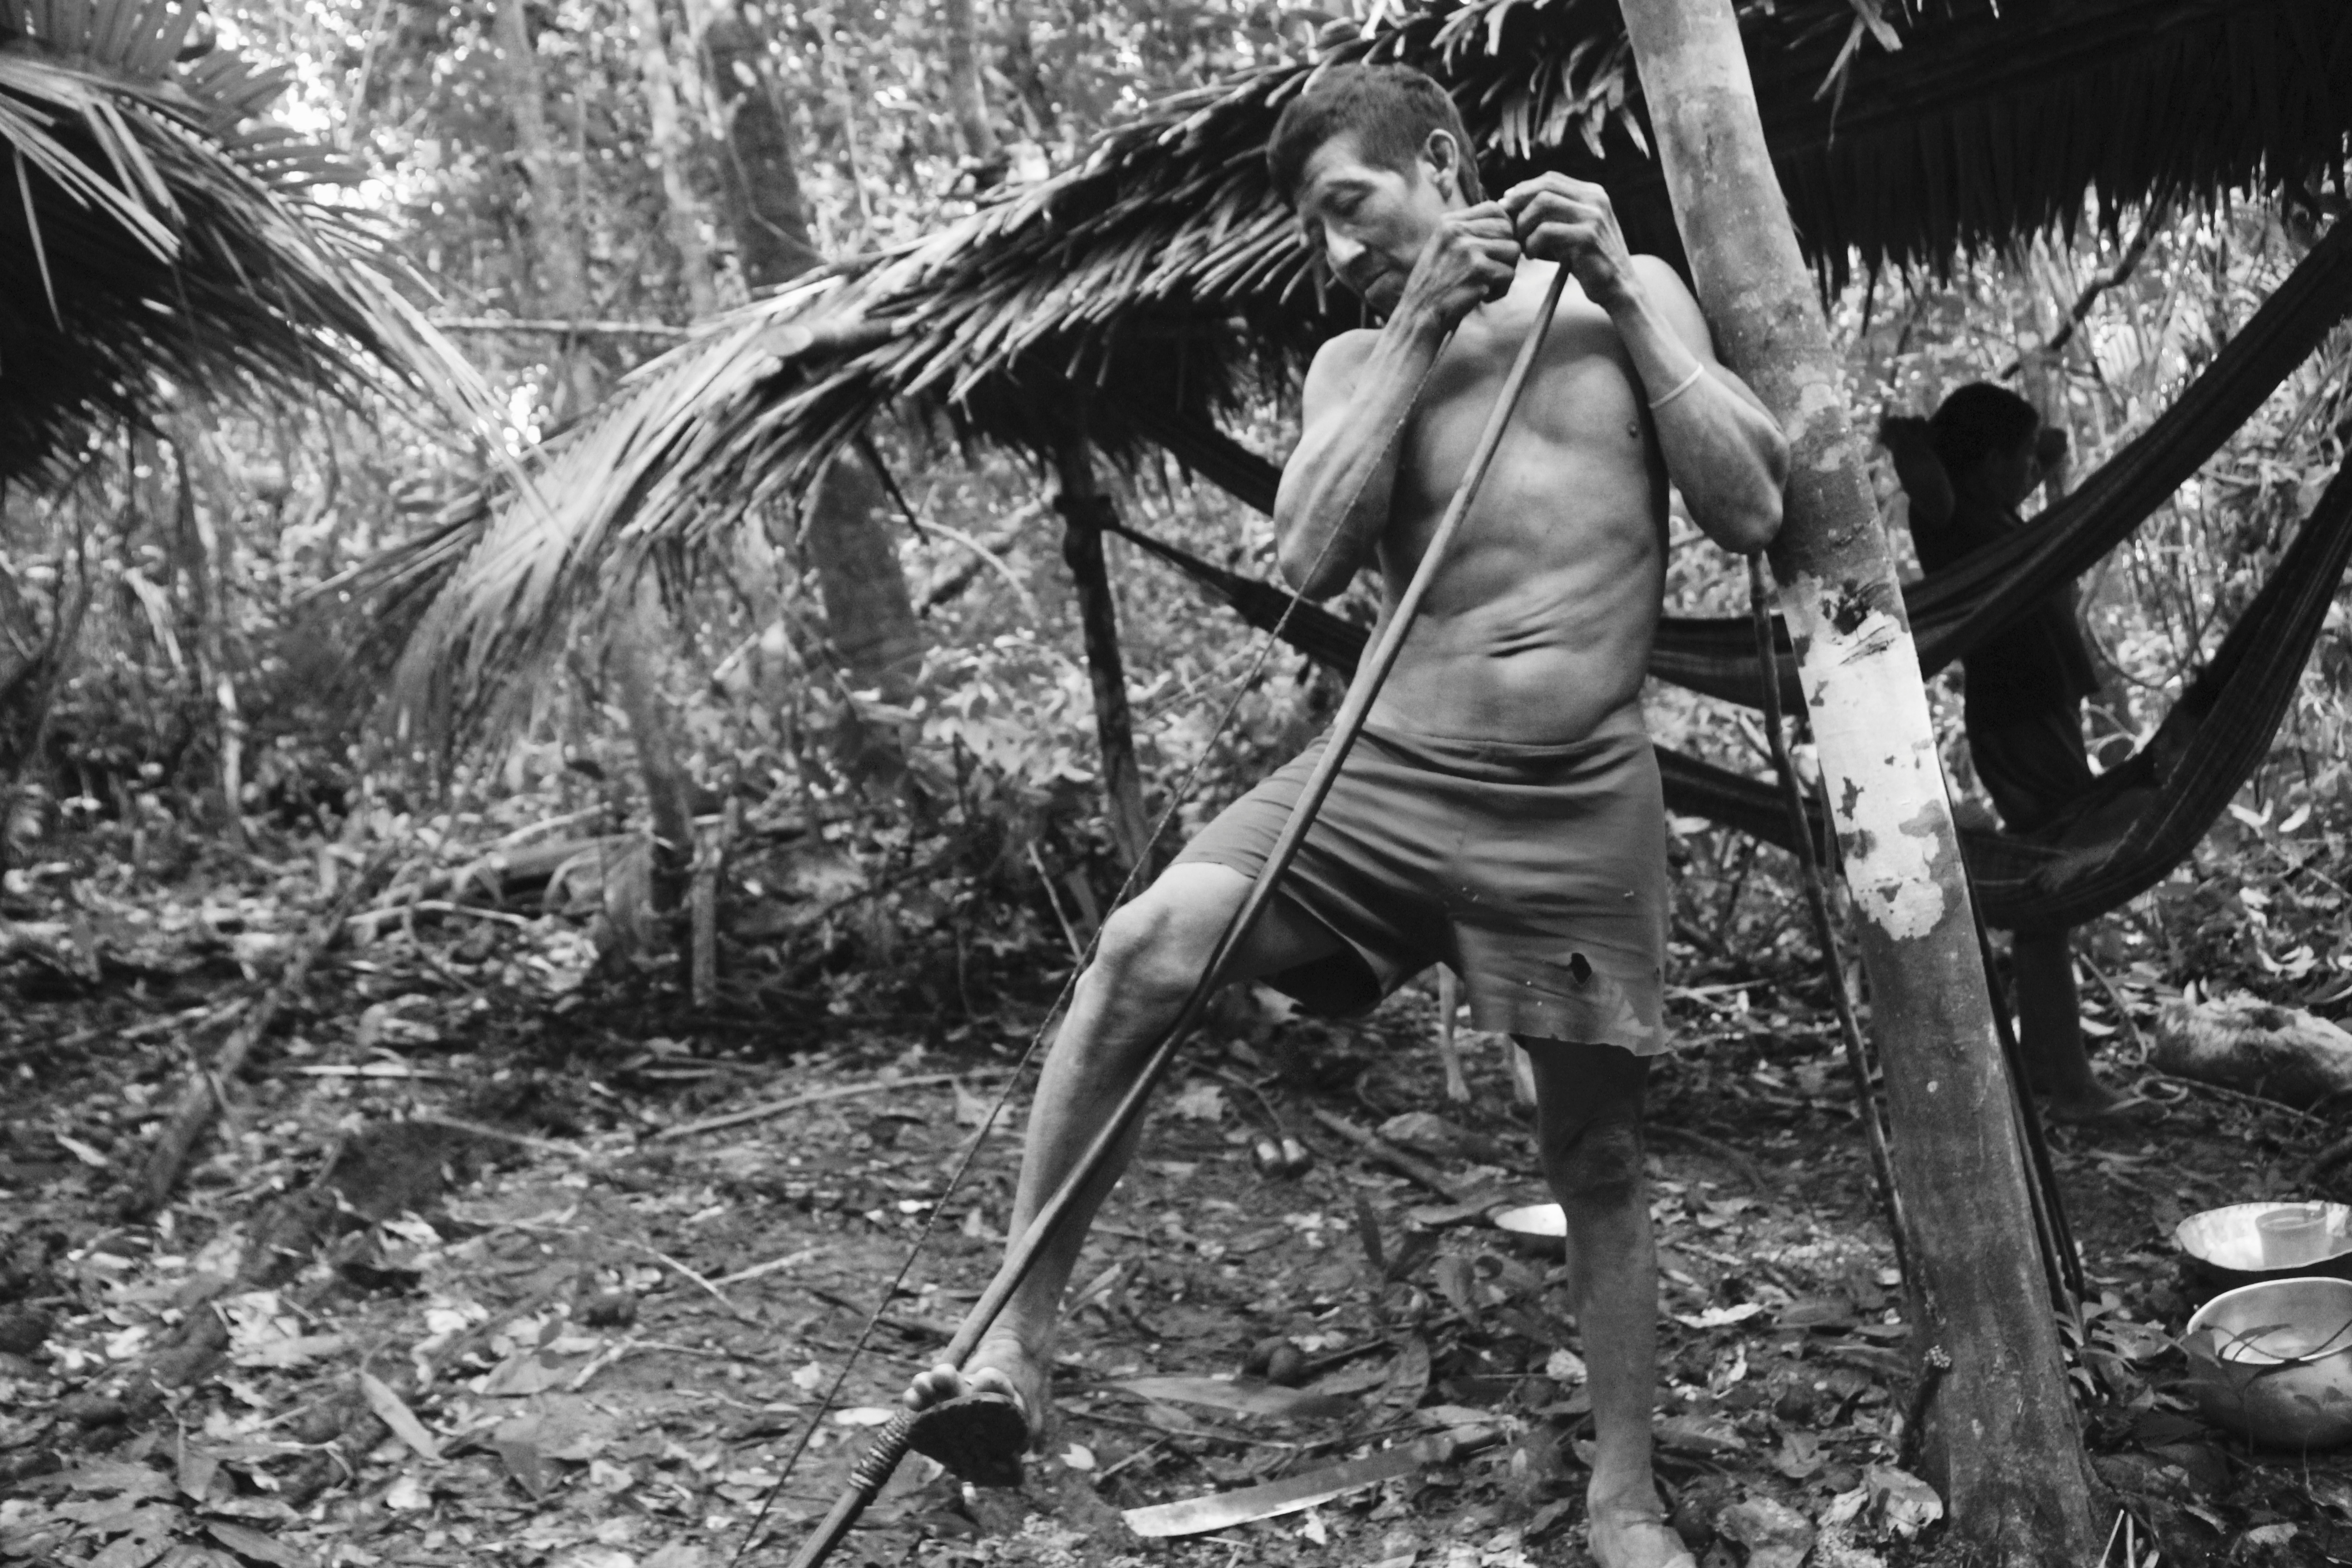
\includegraphics[width=\textwidth]{./imgs/IMG_1669}
%\caption{Takamỹxa'a e seu arco. Ao fundo, na penumbra, sua esposa Irakatỹa descansa no tapiri (acampamento de caça, aldeia Tiracambu, 2013).}
%\end{figure}

Ao sair de suas casas no final da tarde, além de estarem limpos, os
homens levam consigo uma rede (e as cordas para amarrá-la), facas,
espingardas e alguma farinha. Quase sempre dormem à tarde para poder
passar a noite em vigília. Levam também algum pano para se proteger do
frio noturno. Tudo isso, bem amarrado às costas, segue com o caçador até
o local da espera, em alguma das árvores já mencionadas.. Estando lá,
nada na paisagem pode ser modificado; não se pode tirar uma folha de
lugar. A floresta deve ficar o mais intocada possível. O caçador deve
caminhar de leve pelo local para que as folhas não sejam espalhadas, as
pegadas não marquem o chão e o mínimo de galhos secos seja quebrado. Uma
vez escolhida a árvore para a espera, o homem amarrará sua rede no alto
da árvore entre dois troncos firmes --- subindo com a ajuda de caibros
amarrados, tal qual um sistema de andaimes ---, de modo que fique a uma
altura de uns cinco metros do chão, o suficiente para, aliado à
escuridão e ao silêncio, se camuflar. À noite, a floresta é repleta de
sons, e durante a espera noturna o caçador precisa estar com os ouvidos
bem atentos, pois junto com os passos dos animais ouvirá também o grave
som do sapo \textit{kapokapo}; o canto de cigarras e outros insetos; as
folhas remexidas por macacos-da-noite, \textit{aparikya}, e juparás, \textit{haipaxĩa}. 
Ratos, gambás e outras criaturas da noite soltam seus
gritos; o barulho do vento nas folhas das árvores também sonoriza o
ambiente; além dos fantasmas \textit{ajỹ}, que circulam por boa parte da
floresta escura com seus assobios e batidas secas com pedaços de pau nas
árvores.

A espera, \textit{matakwa}, envolve um estado de completa atenção, que
pode ser expresso por termos como \textit{xa} \textit{katy}, ``olhar bem'',
\textit{juanũ}, ``ouvir-atentar'', e \textit{jamaka}, que traduzo por
``prestar atenção''.

E, em que consistiria uma \textit{espera}, \textit{matakwa}, bem sucedida?
Para responder essa questão, listo abaixo os procedimentos e cuidados a
serem tomados durante a \textit{espera} \textit{matakwa} que --- mesmo não
garantindo o sucesso na caça --- são indispensáveis ao bom caçador.

\begin{enumerate}
\item
Não se deve sair de casa suado, sujo, nem exalando qualquer odor, pois
os animais sabem pelo cheiro, \textit{kaxỹ}, que há um humano à espreita
e fogem. O ideal é tomar um banho de rio antes, porém sabão, sabonete,
desodorante ou outros produtos cheirosos dos brancos, \textit{karaia},
não devem ser manipulados. Da mesma forma, estão vetadas as
folhas-remédios, \textit{pohỹ}, extraídas da floresta e que são
utilizadas no tratamento de dores e doenças do corpo, já que seus
odores também espantam as presas

\item
Não se deve pisar em nenhuma fruta, folha ou galho depositado ao pé da
árvore onde ocorrerá a espera, sob o risco de o animal que lá chegar
perceber o rastro humano. Por isso deve-se caminhar sempre descalço.
Os chinelos de dedo devem ser mantidos em casa ou na sacola, \textit{marakũa}

\item
Considerando-se que o caçador precisará construir um andaime para se
\textit{apoiar} e amarrar sua rede com tranquilidade na árvore, os
caibros de madeira a serem utilizados devem ser retirados alguns
metros antes do local da espera, já que nenhum barulho deve ser feito
no entorno da árvore. Além do mais, não poderá haver mudança na
paisagem. Esses caibros são amarrados entre duas árvores próximas, de
modo a formar uma estrutura de três ou quatro níveis que possa dar
acesso a uma altura de cerca de cinco metros do chão. Lá se amarrará a
rede (a rede será amarrada nessas mesmas duas árvores onde se fez o
andaime).

\item
Uma vez o caçador instalado na rede, todos os movimentos devem ser
executados de forma delicada e silenciosa, pois qualquer ruído pode
espantar a caça; seja um leve mexer na sacolinha de munição ou um
\textit{clique} produzido pelo engatilhar do cão da espingarda.

\item
A lanterna --- ferramenta de grande valia na espera noturna --- permanece
amarrada à rede para ser sacada na chegada do animal. Ela é acesa
instantes antes do tiro, apenas para o caçador encontrar a posição da
presa com precisão. O tempo de iluminar a presa é o mesmo em que o
animal percebe que está sendo observado e foge. Os Guajá lembram que
ao ``jogarem luz'' na presa, antes da fuga (principalmente a anta, o
veado e a paca), ela mantém-se paralisada por poucos milésimos,
olhando a fonte de luz. É durante esse tempo que devem atirar.

\item
Dormir está fora de cogitação
\end{enumerate}

Um dos maiores riscos envolvidos nas esperas noturnas é o encontro com
os \textit{ajỹ}. Muitas vezes o \textit{matakwa}, ``espera'', é mal
sucedido, pois os \textit{ajỹ} conseguem dispersar a caça. Os caçadores
contam que muitas vezes os animais são dissuadidos pelos \textit{ajỹ} de
tomarem certa direção para que não morram. Os \textit{ajỹ} espantam seus
animais, dizendo: ``não vão comer naquelas árvores, pois os \textit{karaia}
(não indígenas) estarão lá esperando vocês, eles estão escondidos e vão
matá-los''. \textit{Karaia}, nesse caso, pode ser uma das formas como os
\textit{ajỹ} enxergam os caçadores humanos, devido ao potencial assassino
representado, principalmente, pela espingarda; além do fato de os
humanos, do ponto de vista dos \textit{ajỹ}, encarnarem a
\textit{diferença}, a ``diferença pura'',\footnote{Ver AmaZone, 2010.} uma pura
diferença inimiga.

Em um caso semelhante, ``donos dos animais'' e ``inimigos'' é a forma pela
qual os Araweté pensam os \textit{Ãñĩ}, que, tal como os \textit{ajỹ}, podem
ser definidos como o ``espectro terrestre do morto'' (Viveiros de Castro,
1986, pp.\,216--217). Para os \textit{Ãñĩ} Araweté, os humanos são percebidos
como queixadas. Tal como para os \textit{ajỹ} Guajá, os humanos seriam não
indígenas e/\,ou inimigos. Para os \textit{ajỹ}, os humanos podem ser tanto
parentes distantes com os quais querem manter relações quanto, como
vimos acima, inimigos (não indígenas, ``índios brabos'', dentre outros).
As duas interpretações aparecem quando os Guajá falam dos \textit{ajỹ}.
Ora deve-se manter distância, pois eles querem levar os humanos para
viver com eles; ora porque querem matá-los. A posição de diferença
inimiga (expressa não só pela ideia de \textit{mihua}, mas também de
\textit{karaia}) entre os humanos e os \textit{ajỹ}, no entanto, aparece de
forma bastante nítida quando observada a partir das atividades de caça.
Caso um animal seja alvejado por um caçador e ainda consiga fugir com
vida, são os \textit{ajỹ} que cuidam de suas feridas e os advertem a terem
mais cuidado com os humanos. Como já coloquei anteriormente, os
\textit{ajỹ} mantêm controle sobre algumas espécies de animais de caça
(principalmente os veados, as pacas e os quatis), e são considerados
\textit{jara} desses animais específicos. Como também já discuti, a ideia
de ``dono dos animais'' (pais ou mães da caça, etc.) não apresenta grande
rendimento no caso Guajá, porém não significa que ela não opere
determinadas relações, tal como a dos \textit{ajỹ} com as pacas, veados,
quatis, gambás, ou mucuras (talvez, seu principal avatar, pois também são
chamados \textit{ajỹ}), macacos-da-noite, além de pássaros como o acauã.

O fato de a paca e o veado se alimentarem à noite também está
relacionado à ``proteção'', \textit{riku}, dos \textit{ajỹ} sobre esses
animais, pois a floresta durante a noite --- \textit{pyha}, ``noite''; ou
\textit{matarahỹ}, ``escuro'' --- é mais segura para esses animais. Por
exemplo, Pira'ima'ã me relatou que, certa noite, esteve frente a frente
com uma paca, mas que sua espingarda ``bateu'' --- \textit{pehẽ}, ``quebrar'' --- e
não atirou. Em três tentativas de tiro, a espingarda ``bateu'', dando
tempo suficiente para que a paca fugisse. Pouco tempo depois, Pira'ima'ã
disse ter ouvido de sua rede (na espera) assobios e barulhos de
pauladas, o que indicava a proximidade dos \textit{ajỹ}. O caçador ficou
quieto, sentindo em seguida um arrepio por todo o corpo, seguido de
calafrios\ldots{} era este o sinal da proximidade dos espectros \textit{ajỹ}.

Se hoje toda espera noturna é realizada com espingardas, só conseguirão
realizar essa caçada os homens que manejam essa arma. Os mais velhos,
cuja arma de caça é exclusivamente o arco e flecha, nunca realizam
esperas, embora de alguma forma participem, indicando os bons locais de
caça e dando outras dicas sobre os animais. Ainda assim, as caçadas
noturnas --- \textit{wata} \textit{matarahỹ}, ``andar no escuro'' --- eram
realizadas antes do contato, embora se configurassem mais ativamente
como caçadas terrestres e emboscadas de animais. Naquele tempo, sem
lanternas e espingardas, a possibilidade de esperar um animal com chance
de acertá-lo era muito menor do que hoje. Tochas e lamparinas, feitas a
partir de resinas, principalmente, da maçaranduba, \textit{mixiranỹkaha},
jatobá, \textit{itawa}, jutaí, \textit{itai ihikira}, e amescla, 
\textit{jawarakua}, sempre foram utilizadas como luz, \textit{hawa},
noturna para iluminar os caminhos --- \textit{hape}, ``meu caminho'' ---, nos anos
em que viviam na floresta caçando ou mesmo fugindo. Ainda assim,
conseguem se locomover à noite sem fonte de luz com bastante
competência.

Em uma conversa com Wirahoa, ele me relatou que nasceu e cresceu fugindo
dos \textit{Tenetehara}; que seu pai morreu quando ele ainda era pequeno;
e que sua mãe lhe contava muitas histórias sobre morte entre os Guajá e
sobre a necessidade de seguirem fugindo dos inimigos \textit{kamara} e (os
não menos inimigos) \textit{karaia}. Para tanto necessitavam fugir pelo
escuro da floresta sem carregar qualquer fonte de luz --- somente um tição
em brasa --- \textit{ira} \textit{tata}, ``pau de fogo'' --- para acender fogueiras.
Além de estratégia de sobrevivência, a caça noturna antes do contato só
era possível devido à capacidade que os homens têm de se locomover à
noite, sem luz. Essa capacidade é colocada em prática até hoje, durante
a espera noturna. Nas ``esperas'', muitos animais são alvejados, porém
alguns conseguem escapar, ainda que feridos. Caso percebam a proximidade
de um caçador por causa de sua lanterna, fugirão ainda que esgotem todas
suas forças nessa tarefa. Por isso, até hoje os animais são rastreados
no escuro da mata. Por exemplo, em agosto de 2009, Hajmakoma'ã matou sua
primeira anta. O tiro que ele desferiu não a matou prontamente. Ele teve
de segui-la pelo escuro para capturá-la. Mas mesmo portando uma lanterna
teve de mantê-la desligada, uma vez que a luz poderia pôr a perseguição
a perder. Hajmakoma'ã explicou-me que se o animal enxerga a luz e, mesmo
que esteja prestes a morrer, correrá até seu limite. Mas se não
pressente a presença humana, para e descansa. É nessa hora que será
morto pelo caçador, que estará invisível na escuridão.

\paragraph{Outras esperas}

Além das esperas noturnas em que são utilizadas redes e lanternas,
pequenas esperas em beiradões e igarapés, que também envolvem silêncio e
atenção, são bastante realizadas, principalmente pelos mais jovens que
estão se iniciando nas artes da caça. Estas costumam ocorrer próximas à
aldeia e não exigem que o caçador passe uma noite inteira na mata --- o
que exigiria disciplina e força, que os mais jovens (e muitas vezes até
os adultos) não querem ter.\footnote{Lembro-me de alguns bons caçadores
  da aldeia recriminarem Pinawaxa'a pelo fato de ser um caçador
  incompetente, pois dormia durante a espera e ainda mantinha relações
  sexuais com a esposa, mesmo estando sem sorte na caça, \textit{panemuhũ}
  ``panema''.} Essa espera ocasional pode ser representada pela palavra
\textit{juanũ}, que traduzo por ``atentar'' --- sendo que \textit{nũ} é
``ouvir'', ``escutar'' ---, e requer outros sentidos além da visão --- como a
audição --- como garantia de sucesso na caça. Como muitos animais vão à
noite para a beira do rio beber água --- como a paca e o veado, ou o
jacaré, que lá vive, e mesmo os tatus que vão ``caçar'' minhocas ---, essas
breves caçadas noturnas costumam deixar muito felizes os jovens de 15
anos (que já são hábeis no manejo de uma espingarda). O mais importante
é que consigam caçar no escuro.

Outra forma de ``espera'' bastante utilizada e hoje adotada com algum
entusiasmo é o chamado \textit{badogue}. Um misto de atiradeira e
armadilha --- muito utilizadas pelos moradores que vivem no entorno da
área indígena --- que foi propagado entre os Guajá por eles e funcionários
da Funai. Desde essas poucas décadas de contato, alguns homens já
tiveram duas ou três espingardas pois, devido à utilização intensa da
arma, seu tempo de vida é muito menor do que prevê o fabricante. Chuva,
umidade, lama, quedas, além do feitiço dos animais contra esses objetos,
vários são os fatores que fazem as espingardas se quebrar, muitas vezes
sem chance de conserto. Quase sempre sobra a caixa com o gatilho e o
cão, além do cano, pois a coronha, base do cano e parafusos se perdem
quase que por completo. Quando é possível, os caçadores, com a ajuda de
funcionários da Funai, esculpem novas coronhas, introduzem novas peças e
as adaptam ao antigo cano. Porém, outras vezes os canos ficam sem
utilidade e são readaptados e utilizados na confecção dos badogues ---
arma de caça que consiste em uma estrutura de madeira talhada, na forma
de uma coronha de espingarda, em que é adaptado um cano de espingarda
fora de uso. No corpo da madeira fazem uma câmara conectada ao cano,
onde será colocado o cartucho, e o disparo é feito por um forte tubo de
borracha cirúrgica --- o mesmo utilizado nas atiradeiras de crianças (ou
badogues, bodoques, dentre outros nomes) que conhecemos --- que aciona um
prego cuja ponta, ao bater na espoleta do cartucho, provoca o tiro. Os
badogues são colocados em locais onde se encontram rastros de animal e
servem fundamentalmente para matar pacas, \textit{kararuhua}. Um cabo
(uma linha grossa, ou mesmo fibra de tucum) é esticado de modo a
produzir o disparo assim que é rompido pelo animal, ao passar em frente
ao badogue. Essas armas costumam dar bons resultados, ao mesmo tempo que
(muitas) outras vezes falham, seja por falta de força da borracha ou
porque a espoleta, mesmo provocada, não dispara; ou até pelo fato de o
tiro ser dado, mas não atingir o animal, que estaria fora de alvo.

Outra forma de ``espera'' é a caça de tocaia, \textit{takaja}, que consiste
em uma espera diurna, em que o caçador fica protegido por uma estrutura
de folhas e não é visto pelos animais. A \textit{takaja} é um abrigo de
floresta, formado por uma estrutura de troncos fincados ao chão, de
forma circular, e envoltos por um grosso cipó que proporciona
sustentação às folhas de babaçu ou açaí que revestem o abrigo. O
principal objetivo do abrigo é ocultar totalmente o caçador em seu
interior, além de protegê-lo de eventuais ataques de animais, por isso é
totalmente revestida, do chão ao teto, e seu interior, completamente
escuro. A pouca luz e o ar que recebe provêm de aberturas laterais muito
pequenas, imperceptíveis externamente, e que auxiliam na visão. Ao
passar perto desse amontoado de folhas, os animais não desconfiam da
armadilha e são surpreendidos por um tiro ou flecha. Adultos e crianças
armam \textit{takaja}, sendo esta, inclusive, uma das formas com que um
jovem se inicia nas caçadas. Meninos ainda muito jovens, entre oito e 10
anos, armam pequenas \textit{takaja} na floresta, próximo à aldeia, e com
auxílio de suas pequenas flechas e atiradeiras conseguem abater
inhambus, mutuns-cavalos, jacus, jacamins, juritis e até mesmo pequenos
mamíferos, como o quati-puru, \textit{tamakaja}, e a cotia, \textit{akwixia}.

Uma \textit{takaja} pode ser construída tanto no solo (para a caça de
animais terrestres) quanto no alto das árvores, quando o objetivo é
caçar pássaros que se abrigam nas copas, como o tucano-de-bico-preto, \textit{takỹna}, 
específico da região, e o araçari --- \textit{takyynihĩ},
``tucaninho'' ---, aves importantes cujas penas são matéria-prima para a
confecção dos diademas e braceletes utilizados pelos homens. As
\textit{takaja} feitas no alto das árvores podem ser montadas a grandes
alturas, de até 20 metros. A que vemos na foto foi feita por um caçador
experiente com a ajuda de seu cunhado. O homem subiu na árvore
carregando cipós --- um, inclusive, bem longo que, lá de cima, alcançava o
chão. Uma vez no alto, lançava o longo cipó para Juxa'a que o amarrou a
finos troncos de árvores (seis troncos foram necessários), depois folhas
da palmeira açaí e mais cipós, em várias subidas e descidas, tal como um
elevador de cargas. Em menos de uma hora, a \textit{takaja} estava pronta
lá no alto.

%(\textbf{foto da tocaia})
%\begin{figure}[H]
%\centering
 % \includegraphics[width=\textwidth]{./imgs/IMG_1615}
%\caption{Auxiliado por seu cão, Maihuxa’a caça uma cotia no buraco (acampamento de caça, aldeia Tiracambu, 2013).}
%\end{figure}

\section{palavras noturnas}

Não poderia deixar de mencionar aqui as palavras noturnas que, ao final
de um dia, consagram não só as caçadas, mas toda a vida. É à noite que
as pessoas comentam sobre os acontecimentos do Posto Indígena; sobre a
atitude de determinados funcionários; a preocupação com os invasores da
área; e tomam decisões que levarão aos funcionários da Funai sobre
determinado tema, tal como uma ``política noturna'' (nas palavras Peter
Gow), que deve ser realizada cotidianamente. Além dos assuntos
cotidianos, minha presença na comunidade alterava o teor das conversas,
quando me sabatinavam sobre o mundo dos \textit{karaia} com perguntas,
como: se eu conhecia o então presidente Lula ou a liderança indígena
Marcos Terena; se em São Paulo havia Guajajaras; se meu sogro não se
zangaria por eu deixar minha esposa e filha sozinhas por tanto tempo; e
mesmo se eu não estava pensando em me casar com alguma mulher da aldeia;
--- dentre tantas outras questões que eu respondia, buscando compensar
minhas interpelações diárias e invasivas. Tudo ocorria sob o olhar
atento das crianças, a desconfiança dos velhos e o vigor dos jovens ao
perguntar, explicar, e tornar a perguntar. Além das caçadas, o tema que
mais causa comoção nas conversas noturnas são os invasores da área, cujo
impacto na vida das pessoas é óbvio. Os Guajá planejam ataques, ameaçam,
puxam arcos e marretas enquanto falam, prontos a matar um inimigo que
parece estar ao lado do narrador. Caça e guerra aparecem nas conversas
noturnas. E as noites sempre eram mais animadas graças a essas
narrativas.

Desde a volta do mato, quando chegam na aldeia, comentários e
brincadeiras já começam a ilustrar aquele dia de caçada. Há um tipo de
comentário bem-humorado feito quando alguém retorna, quase sempre
proferido por outro que, em um primeiro momento não se beneficiará da
comida, muito provavelmente um afim distante, assim: ``Ah, você trouxe
caça para mim meu irmão'', ou ``filho'', \textit{haxa'a}, ``hoje eu vou comer
muito bem meu irmão''. Muitas gargalhadas são dadas, pois a caça em
questão não é para a pessoa que comentou, tampouco ela tem esse grau de
parentesco com o caçador. São piadas como essas ou cantos sobre
determinado \textit{karawara}, ``caçadores'', que marcam a chegada das pessoas
nas aldeias. Porém, é à noite que as caçadas cotidianas são lembradas, e
por vezes toda a assembleia de uma aldeia estava atenta a uma única
pessoa, que contava os feitos do dia como se narrasse belos mitos. Essas
falas podem ser chamadas \textit{muumu'ũ}, ``narrativas'', ou, como outras
conversas cotidianas, ``falas'', \textit{ma'iha}. Uma das experiências
estéticas mais fascinantes durante meu trabalho de campo foi poder ouvir
pessoas narrando e comentando caçadas, em um ritmo pausado, marcado por
silêncios e cadências que ressaltavam as situações, além de onomatopeias
e imitações magistrais, tal como ``imagens de sons'' (Kohn, 2013, p.\,36).
Descola observa, para o caso Ashuar, que ``graças às intermináveis
histórias de caça que os homens gostam de contar, todo mundo também sabe
qual foi o comportamento do animal antes de morrer: o medo, a tentativa
de fuga abortada, o sofrimento, as manifestações de aflição dos seus
companheiros. Em suma, ninguém pode ignorar de que maneira um ser vivo
se torna comida'' (Descola, 1998, p.\,29). Entre os Guajá, não só os
homens narram caçadas, mas é muito comum as mulheres serem ouvidas por
todos, quando complementam seus maridos ou mesmo protagonizam, por falas
exclusivas, seus feitos na mata. Os relatos --- \textit{ma'iiha}, ``fala'' ---
sobre as caçadas são ilustrados por imitações de sons de animais,
batidas e movimentos de mãos e pés. A mesma capacidade que os Guajá têm
para imitar os animais visando à predação é aqui utilizada para ilustrar
realisticamente a experiência do caçador. Essas narrativas não seriam
exclusivamente sobre ``caçadas'', mas remetem a uma experiência total, com
referência à extração de mel, passagem por antigos acampamentos, ataques
de \textit{ajỹ}, dentre outros eventos --- tudo o que estiver relacionado ao
\textit{wataha}, à ``caminhada''.

À noite, e mesmo durante alguns dias seguidos, um caçador pode se reunir
com outros e contar suas proezas: vangloriar-se de como enganou uma
paca; comentar sua paciência durante a espera de um veado; a boa
estratégia na emboscada a um bando de capelães; a forma como o vento
dificultou sua audição durante a perseguição a uma ave; a resistência a
mordidas de muriçocas em uma noite quando esperava uma anta em um pé de
pequi; a alegria de saber que o jacaré que mergulhou, após ser ferido de
raspão, emergiu morto à superfície; o encontro com os \textit{ajỹ} durante
uma espera noturna, quando o caçador na madrugada fria soube manter a
calma e não se apavorar, esperando os espectros se dissiparem,
demonstração de grande coragem e sabedoria; a mordida de uma valente
cotia que se escondeu no fundo de um buraco já devastado (mas lá
resistia), e de como, mesmo ferido, o caçador aguentou a dor da mordida,
agarrou-a pelo pescoço e conseguiu asfixiá-la; a flecha certeira, o tiro
perdido, a pólvora molhada\ldots{} tudo é lembrado à noite, à meia-luz, sob o
embalo de comentários atentos, risonhos e curiosos.

Estes e outros acontecimentos --- ora insignificantes, ora fantásticos ---
compõem a vida de um caçador. Seus momentos de embate, no entanto, não
devem ser lembrados com remorso nem tristeza, ao contrário, com orgulho
e regozijo. ``Eu sou melhor do que uma onça, não tenho medo dela'',
disse-me certa vez Pira'ima'ã depois de, orgulhoso, me mostrar dois
caninos de uma onça pintada que ele havia matado. ``Se ela tem unhas, eu
tenho a minha espingarda. Quando eu percebo uma onça no mato, eu a chamo
bem alto, `pode vir bicho, eu tenho uma espingarda e vou te matar!'" E
a onça, vista como bicho --- \textit{hama'a}, ``minha caça'' ---, se torna menos
perigosa.

Ao iniciar minha pesquisa, não entendia de que se tratava aquelas
conversas tão compenetradas. Nada fazia sentido. Somente quando passei a
acompanhá-los nas caçadas pude perceber que elas sempre eram remontadas
em fala, redramatizadas. Lembro-me de uma específica vez em que
Hajmakoma'ã reproduziu o som de uma vara de porcos chegando ao longe,
sua boca ainda fechada foi se abrindo aos poucos, o que dava a real
sensação de que os animais estavam cada vez mais perto, se aproximando.
Em seguida, surgiram sons de folhas remexidas, dentes e rugidos. À
medida que ele narrava, novos sons apareciam, cada vez mais altos, até o
momento em que imitou o som de um tiro certeiro que mata um animal, e o
silêncio se restaura. É certo que eu não entendia nada daquelas
conversas, pois nessas horas os Guajá falam muito rápido e com a ajuda
de estalos, urros, gritos, assobios, como se a natureza do evento
penetrasse na palavra. Lima aponta o mesmo espanto ao descrever as
conversas yudjá que antecedem uma caçada de porcos: ``em um instante já
não posso compreender o que os caçadores dizem. Todos falando ao mesmo
tempo, gritos estridentes, onomatopeias de explosões de tiros, flechas
silvando, porcos batendo os dentes, porcos em correria. Todos têm casos
para contar e mímicas para fazer'' (Lima, 1996, p.\,22).

Ao ouvir sobre as caçadas, as pessoas ao redor muitas vezes parecem não
prestar atenção no que diz a boca do caçador. É comum o narrador parecer
estar falando com ninguém, todos mais preocupados em comer, descansar,
olhar para outro lado. Para participar da narrativa, as pessoas não têm
de estar necessariamente paradas, absortas pelas palavras, olhando o
narrador de forma fixa.\footnote{Dispositivo discursivo análogo ao de um chefe
ameríndio, cujas palavras nunca se transformam em voz de comando, tal
como sublinhou Pierre Clastres.} Trata-se de uma maneira de narrar, uma
forma de falar e ouvir os acontecimentos da vida que, no início, dado
meu despreparo etnográfico, cheguei a cogitar que fossem mitos, pois
todos, adultos e crianças, estavam muito envolvidos, embora parecessem
desatentos, juntos, como se aos mais jovens estivessem sendo narradas
fábulas fantásticas, de lugares outrora vistos apenas por poucos seres
no mundo e experiências que os humanos não mais conhecem. Mas os Guajá
não narram mitos, como narram caças. Preferem falar das caçadas e mesmo
de antigos eventos, a mitos. Discursos que versam sobre o desespero por
terem perdido uma trilha, \textit{pea}, e a alegria de reavê-la; o choque
pelo encontro com uma onça ou fantasma e o alívio de retornar à casa,
com saúde e comida. Histórias por si só prodigiosas e que, devido às
formas poéticas, soavam ao etnógrafo como mitos. Os Guajá -- e, penso,
talvez, a maior parte dos povos ameríndios --- não depositam na cosmologia
e na mitologia algo como um repertório narrativo que deve ser proferido
esporadicamente, como se isso salvaguardasse a \textit{sociedade} e fosse
uma transmissão de saber ou qualquer outra forma de \textit{socialização}
(nós, sim, fazemos isso!). O mundo --- composto por viagens ao céu;
caçadores celestes; fantasmas na mata; relações sociais entre os
animais, dentre tantas outras características --- é dessa forma, e não
precisam lembrar a ninguém que ele é assim. Aqui as pessoas não passam
seus dias falando sobre o céu e os mortos. Ao contrário, e ao menos para
os Guajá, o que faz de uma conversa algo interessante são os episódios
dramáticos da vida presente; que falem de comida ou do dia de caça que,
por si só, já são extraordinários.

A narrativa é contínua à caça, e está diretamente relacionada às formas
com que as pessoas atuam na floresta muito mais do que uma interpretação
isolada de uma ideia abstrata de caça e caçada. Ao contrário, relata-se
uma caçada específica, e não uma idealização. Tal como observa Ingold
para as múltiplas produções de significado a respeito do espaço e
atividades nele envolvidas (Ingold, 2000, p.\,56) --- e como já colocado
anteriormente --- em casos como o dos Guajá, separar a atividade de caça
de atividades como narrar as histórias e cantar seria tirar tais
narrativas que estão \textit{no} mundo (produzindo-o, inclusive) e as
colocar como uma interpretação \textit{da} natureza --- algo que elas não
representam; tal como sua ideia de \textit{enskilment}, com que o autor
nos mostra o quanto fazer e aprender são processos inseparáveis para
muitos povos. No caso Guajá, ao passo que todos riem e ficam apreensivos
com as narrativas de caça, também visualizam o tamanho do animal, a
configuração da paisagem, as decisões do caçador, dentre outras
informações que só aparecerão com a narrativa. As narrativas dos
caçadores Guajá enfatizam quanto suas presas se desesperaram ao vê-los;
\textit{inimigos}, \textit{mihua}, que eram, ao mesmo tempo tais narrativas
consagram (lembrando os argumentos de Lima para a caça yudjá) a
\textit{vitória da perspectiva dos humanos} (que prescrevem a caça) sobre
a perspectiva do animal caçado (que prescreve a guerra), pois o
contrário será sempre desastroso, como veremos agora. Tudo se passa como
se a caçada ainda não tivesse terminado. Aqui, ``a palavra é caça'' (Lima,
1996).

\section{\textit{ha'aera e panemuhũ}, «sobre isso não sabemos»}

A caça é uma atividade que envolve perigo, tanto em sua complexidade
técnica (já que é extremamente desgastante, com o caçador sujeito a ser
atacado por animais, machucar-se de várias formas e mesmo falecer)
quanto pelo fato de muitos animais caçados serem dotados de
\textit{ha'aera} e, a partir disso, se vingarem dos humanos. O
\textit{ha'aera} é o mesmo princípio nocivo e raivoso que compõe a pessoa
Guajá (como vimos no capítulo 2) e que, após a morte, se transubstancia
no formato \textit{ajỹ}. No caso dos animais, o \textit{ha'aera} não se
transforma em \textit{ajỹ} --- isso só ocorre com o \textit{ha'aera} humano ---,
mas está próximo ao que a literatura etnológica sul-americana denomina
como ``vingança'' (animal e/\,ou canibal) e termos congêneres.\footnote{Ver Lima,
1996; Hugh-Jones, 1996; Viveiros de Castro, 2008.} No que concerne à
caça, o \textit{ha'aera} pode ser lançado aos humanos por animais mortos,
pelos fantasmas \textit{ajỹ} e até mesmo por humanos mortos. Assim me
falou Wirahoa:

\begin{quote}
Quando vamos matar os capelães, eles ficam muito aflitos, pois pensam
que nós somos madeireiros. Após comermos sua carne, um deles vem durante
a noite, enquanto estou dormindo, e me diz: \textit{você me matou né, seu
madeireiro? Agora vou jogar minha raiva (ha'aera) em você}.
\end{quote}

E, no dia seguinte, o homem pode acordar doente, com febre, indisposto.
Mesmo que goze de alguma saúde, pode experimentar um completo estado de
azar em sua vida. O \textit{ha'aera} pode atingir mulheres e crianças.
Nesse caso, quase sempre lhes causam doenças. Quando atinge e se aloja
nos homens, pode ser chamado \textit{panemuhũ}, termo que pode ser
traduzido por ``panema''.

Em um sentido lato, a ideia de \textit{panemuhũ} faz referência a um
conjunto de circunstâncias e estados que vão desde um mal-estar --- como
uma indisposição, dores e cansaço excessivo ---, passam por doenças mais
graves e chegam até mesmo à perda do \textit{haitekera}, o princípio
vital. Uma vez \textit{panemuhũ} --- irritado, fracassado e sem paciência
---, o homem deve permanecer só em sua rede até que as coisas melhorem. Os
Guajá não gostam de conversar sobre o \textit{paneemuuhũ}, tal como fazem
com outros assuntos --- como o \textit{iwa}, os animais, ou mundo dos não
indígenas. O assunto em si já deve ser evitado, e o mais comum quando
falávamos sobre o tema era eu ouvir ``É assim mesmo!'' ou ``Não sei não, eu
não lembro!'' ou ainda ``Pergunte para outro!'' Como se o fato de falar e
admitir o \textit{panemuhũ} fosse propiciá-lo. Por isso, as informações
abaixo diferem de outras que constam neste trabalho; são fruto de pura
observação e interpretação, e não de conversas animadas e interessantes,
tais como as que mantive sobre outros temas.\footnote{Algo muito parecido
  foi observado por Clastres em relação aos Guayaki. O autor informa que
  seus interlocutores tinham ``pouca prolixidade'' quando tratavam do
  \textit{pane}, termo cognato ao \textit{panemuhũ} Guajá: ``O que é
  \textit{pane}? Sob aparência anódina, essa pequena palavra perigosa
  designa de fato a pior das coisas que pode acontecer a um índio: a má
  sorte na caça'' (Clastres, 1995, p.\,19).}

Em sentido estrito, o \textit{panemuhũ} seria análogo à ideia de ``panema'',
o \textit{azar na caça} e outros infortúnios, tal como conhecido por
diversas comunidades tradicionais do Norte brasileiro (Galvão, 1976;
Matta, 1973; Wagley, 1988; e para um caso ameríndio, Clastres, 1995),
tendo sido discutido recentemente por Almeida (2007). Mesmo os Guajá
podem se referir a seus ``azares'' pelo termo \textit{panema}, em
``português'', tal como aprenderam com os \textit{karaia} nesses anos de
contato, que traduz de forma muito satisfatória o (termo cognato)
\textit{panemuhũ}. É muito comum um homem voltar calado da floresta e, ao
chegar em casa, comentar em português ``\textit{Tô panema}!'', como se
dissesse que a caçada foi improdutiva, ou mesmo como um sinal de que
algo pior havia acontecido. Mas, o que ocorre de fato nessas situações?
O que, além da morte, pode ocorrer de tão ruim a um caçador na floresta?

O estado \textit{panemuhũ} que acomete um caçador é, quase sempre, no
cotidiano o resultado de uma \textit{vingança} animal, isto é, uma
descarga de \textit{ha'aera} oriunda de algum animal abatido. Os
\textit{ajỹ} também, decerto, podem lançar o \textit{ha'aera} em um humano,
deixando-o doente e/\,ou \textit{panemuhũ}. Veados, macacos, antas,
capelães, porcos, cotias, tatus, dentre outros animais, são dotados de
um \textit{ha'aera} violento. Desta forma, com uma formulação simples, o
\textit{panemuhũ} seria um estado circunstancial que um caçador (mas não
só um) experimenta após o ataque de um \textit{ha'aera}, seja ele
produzido pelos animais abatidos ou ex-humanos \textit{ajỹ}.

Além disso, há um conjunto de atitudes e pequenos eventos que podem
produzir uma exclusiva má sorte na caça e que nem sempre está
relacionado ao potencial assassino do \textit{ha'aera}. Em outras
palavras, \textit{panemuhũ} pode ser tanto um sintoma grave de um ataque
espectral e assassino, relacionando-se à saúde e composição de uma
pessoa, quanto um azar momentâneo resultado da quebra de uma regra ou
prescrição menor (algo como uma ``quebra tabu''). Existiriam, como em tudo
na vida, graus de azar\ldots{} e sorte, coragem, medo, alegria, tristeza\ldots{}
Da mesma forma, Clastres observa que o \textit{pane} entre os Guayaki era
evocado ``a propósito de circunstâncias ora graves, ora fúteis de sua
existência cotidiana'' (Clastres, 1995, p.\,18).

Se um homem permanece durante sucessivas caçadas matando apenas pequenos
animais (tal como aves menores, tatus, roedores) ou mesmo capturando
apenas jabutis, ele deve se preocupar, pois pode estar \textit{panemuhũ},
uma vez que as grandes caças podem ter desaparecido. Assim, podem
provocar o \textit{panemuhũ}: 

\begin{enumerate}
\item Um acesso de raiva (ou a raiva contida)
\item Tristeza ou aborrecimento de uma esposa em relação a seu marido
\item Saudade e lembranças de alguém
\item Qualquer outro sentimento que altere
o humor do caçador ou de alguém para com o caçador, tornando-o
``triste'', \textit{kije} --- notem que \textit{kije} é um termo cuja tradução
pode ser medo e/\,ou tristeza, sentimentos que neste contexto são
experimentados de maneira simultânea a partir da ideia de um
``medo-tristeza''
\item Cócegas, \textit{kiinihĩ}, feitas por uma esposa ou
filhos nas axilas de seu marido, ou pai, pois ele perderia a firmeza no arco
ou na espingarda, seus braços ficariam ``moles'' e ele se tornaria
\textit{panemuhũ}
\item Caçar após o nascimento de um filho, pois esse pai,
além de não matar nada, pode enlouquecer; caso um homem vá caçar no
período de resguardo do nascimento do filho, um calor intenso se
apossará do seu corpo, um prenúncio da loucura
\item Em alguns casos (como
as caçadas de espera noturna), anunciar que está indo à mata pode causar
panem, pois os animais ``ouvem'', \textit{nũ}, e, por isso, sabem, 
\textit{kwaa}, que serão caçados
\item Alguns sonhos, como os cobras, também podem deixar o caçador sem sorte
\end{enumerate}

Além destas, há várias prescrições de ordem sexual e de atitude que
engrossam esta lista. Em linhas gerais, quando um homem está
\textit{panemuhũ} ele tem dificuldades de encontrar animais para caçar
(embora os animais não alterem seu ciclo), e é muito comum ele caminhar
durante todo um dia e não encontrar presa alguma; caso encontre, é bem
provável que não a mate. Os bichos simplesmente ``desaparecem''. É um
estado que, tal como uma doença, a pessoa que a contraiu sente. Nesses
casos, ele deve voltar para casa, falar com sua esposa o que está
havendo e descansar, pois quando o \textit{panemuhũ}, ou \textit{ha'aera}, é de
um tipo fraco ele tende a passar.

Trata-se aqui de ``um conceito altamente abstrato, como gravidade'',
como observa Almeida sobre a complexidade da ideia de ``panema'' entre
seringueiros do Acre --- uma ideia que envolve mecanismos e regras
particulares que, por sua vez, põem em relação uma ontologia diferente
da ``nossa ontologia naturalista que distingue domínios naturais e
domínios morais'', constituindo-se uma ``economia ontológica da caça'':

\begin{quote}
(Panema) é um estado que é sentido no corpo, assim como sentimos um
peso; {[}\ldots{}{]} Panema, exatamente porque é tão generalizado como a
gravidade, e tão difuso como a honra pessoal, é algo que se confirma a
todo o momento pela experiência. Tudo se passa, de fato, como se panema
fosse parte do mundo. (Panema é um componente generalizado da
ontologia de caçadores da planície amazônica; e é confirmado-corroborado
por encontros pragmáticos cotidianos. Para meu pai, que na infância
viveu na mata com meu avô seringueiro, e depois tornou-se bancário de
carreira, assim como para o líder político e sindical Osmarino Amâncio,
panema nada tinha a ver com superstição, ou com religião, que ambos
rejeitavam por razões diversas. Panema era um fato do mundo, que a
experiência confirmava.)\footnote{Almeida, 2007, pp.\,08--09.}
\end{quote}

Um ``fato do mundo'', confirmado pela experiência, também me parece uma
excelente definição para o \textit{panemuhũ} awá-guajá, uma vez que tal
estado é sentido e experimentado por todos em um ou outro momento, em
diferentes situações de vida.

\section{nem tudo é azar}

Embora me faltem elementos suficientes, gostaria de lembrar que, assim
como alguns eventos e fatores desestimulam uma boa caçada, outros podem
ajudar. Desta forma, alguns sonhos são propiciatórios, como sonhar com
onças; já que, segundo Pira'ima'ã, a onça é um grande predador, e vê-la
em sonho pode ser sinal de que o caçador, ele mesmo, vá matar muitos
animais. Não sei se é uma regra geral, mas, ao menos para Pira'ima'ã,
sonhar com onças é um dos melhores prenúncios para uma boa caçada.

Muitas vezes os Guajá abatem fêmeas prenhas e, em todos os casos, os
fetos são consumidos como iguarias. Fetos de cotia, de capelães, além de
porcos e de antas são muito apreciados. No caso de quase todos os
grandes animais fêmeas em adiantado estágio de gestação (principalmente
antas, queixadas e caititus), as pessoas lavam a mão no líquido
amniótico da placenta, ao retirar o feto morto. No caso da anta, obtive
duas explicações pare esse procedimento: primeiro, que o líquido chamado
\textit{imymy} \textit{tekwera}, ``líquido da criança dela'', ``educaria'' a mão
do caçador para que ele mate mais antas; depois, que ele fortaleceria o
corpo de quem lava as mãos, uma vez que o couro da anta é bem duro. Em
todo caso, me justificaram que lavam a mão no líquido amniótico de
outros animais como um procedimento propiciatório, e que isso atrairia
mais caça. Pode-se lavar as mãos no líquido amniótico de diversos
animais, porém isso quase nunca ocorria quando matavam caças pequenas
(capelães, macacos, cotias). Era mesmo um ``procedimento propiciatório
ocasional'' (já que os Guajá, avessos a cerimônias, não praticam ritos de
caça ou caçadas rituais).\footnote{É importante enfatizar que, embora
  apreciem comer carne de ``vitelas'', os Guajá não têm predileção
  especial por matar fêmeas grávidas; ao contrário. Foi com pesar que,
  certa vez, Wirahoa recebeu a notícia de que a anta que seu irmão
  Hajmakoma'ã matara estava prenha e o filhote, prestes a nascer. O
  filhote já estava bem formado e até malhado, com são os filhotes de
  anta. Disseram-me que, em casos como esse, retiram logo o filhote da
  mãe recém-morta para os tomar como animal de criação. Como aquela foi
  a primeira anta que Hajmakoma'ã matou, ele não teria tido a habilidade
  necessária para salvar o filhote.}

Em outra ocasião que também envolvia a caça de uma anta, após chegar ao
local onde Pira'ima'ã havia matado o animal horas antes, seu amigo
Pinawaxa'a deu alguns tiros no corpo do animal morto, gritando ``venha
anta, venha que eu vou matar você''. Pouco depois outro homem, Kamara,
chegou ao local e flechou por várias vezes a anta com uma taboca. Disse
que era para dar sangue para sua flecha e pela vontade --- \textit{xaku'uhy},
``ver-querer'' --- que também sentia de matar antas. De certa maneira, embora
estejamos falando sobre caça, isto remete a uma passagem de Descola
sobre a guerra ashuar, quando diz que ``a morte de um inimigo é assunto
coletivo: assim que um membro do grupo dá o tiro mortal, todos
descarregam as espingardas sobre a vítima abatida e se tornam, por esse
ato, coassassinos solidários, de modo que os jovens ainda inexperientes
começam desde muito cedo a acumular façanhas'' (Descola, 2006, p.\,346).
Talvez seja por isso que eu não mais me surpreendia quando chegava à
aldeia, voltando de uma caçada junto com determinado grupo (todos nós
carregando aves, macacos, pacas, cotias e, por vezes, quilos de carne
moqueada), e quem estava no pátio (e não havia estado na floresta) me
rodeava para ver o que eu trouxera, perguntando ``o que \textit{você}
matou, Uirá?'', embora eu não tivesse dado um tiro sequer; ou à noite,
quando estávamos comendo, me incluíam como responsável pela morte do
animal que estávamos consumindo. Nas caçadas de que eu participava,
mesmo não matando uma presa sequer, eu era tido como um responsável, com
se eu fosse --- parafraseando Descola --- um cocaçador solidário. No início
pensava tratar-se de apenas um gesto de generosidade, do tipo ``nós
aceitamos você aqui!''; porém, aos poucos fui percebendo que assim
acontecia com outras pessoas. Por isso mesmo, talvez uma das maiores
indelicadezas que alguém possa cometer é se vangloriar de ser melhor
caçador do que outro; ou se vangloriar de feitos que, todos sabem, são
coletivos. Quando um homem vai mal na caça, não é por uma incapacidade
``natural'' como ``falta de talento'' --- tal como nós justificamos nossas
habilidades e a falta delas --- mas porque deve estar fazendo as coisas de
forma equivocada, já que se as fizer da maneira correta poderá ter
sucesso. Era assim com um finado amigo da aldeia juriti, considerado um
``mau caçador'' por muitos. Não que ele não soubesse caçar, ao contrário;
mas é porque ele quebrava diversas prescrições fundamentais ao bom
caçador --- por exemplo, mantinha relações sexuais de forma desmedida
(mesmo que à força) com muitas mulheres da aldeia e em seguida queria
caçar; mesmo estando doente, ia para a floresta; dormia na espera; não
cuidava bem de suas armas de caça --- muito mais do que seria um caçador
sem talento; para os Guajá, um ``mau caçador'' é aquele que não obedece as
regras do jogo.

\section{\textit{ha'aera}, «aqui tudo é azar»}

Voltemos porém ao \textit{ha'aera} que, ao que tudo indica, é a principal
causa de \textit{panemuhũ}.

Um dos principais e mais devastadores efeitos do \textit{panemuhũ} é o
poder de desconectar a pessoa de seu princípio vital, de sua
``vitalidade'', o \textit{hajtekeera}. Uma clássica ``perda da alma'', em
termos xamânicos amazônicos, já foi bem discutida por alguns autores
(para um balanço, ver Viveiros de Castro, 2002, pp.\,345--399). É esse mal que
a vingança dos animais, \textit{ha'aera}, e dos \textit{ajỹ} produz nos
seres humanos. Se pensarmos o \textit{panemuhũ} a partir da fisiologia da
pessoa, awá, da relação entre os elementos \textit{hajtekeera}, 
``princípio vital'', \textit{ha'aera}, ``raiva'', e \textit{ipirera}, suporte físico, 
``corpo-pele'', veremos que pressupõe um
enfraquecimento, muitas vezes um abandono do \textit{hajtekera} (o
princípio vital), devido a algum trauma --- como um susto ou uma grande
dor --- sobre o \textit{ipirera}, o corpo, ou mesmo um elevado acúmulo de
\textit{ha'aera}, ``raiva'', no corpo, provocado por mau-humor
--- \textit{imahy}, ``braveza'' --- ou tristeza --- \textit{kije},
``medo-tristeza''. Desta forma, um dos piores males a acometer um
caçador (e em consequência, sua família) é ele receber uma grande dose
de \textit{ha'aera} como vingança de uma presa abatida, capaz, inclusive,
de expulsar seu \textit{hajtekera} do corpo e deixar em troca o
\textit{panemuhũ}. Em linhas gerais, um homem se torna \textit{panemuhũ}
e ou doente quando se distancia de seu princípio vital (seu
\textit{hajtekera}). Se imaginarmos o \textit{panemuhũ} a partir da
fisiologia da pessoa guajá --- da relação entre \textit{hajtekera}, 
``princípio vital'', \textit{ha'aera}, ``raiva'', e \textit{ipirera}, suporte
físico, ``corpo'', como vimos no capítulo 3 ---, os Guajá sugerem que o
\textit{panemuhũ} pressupõe um enfraquecimento e, muitas vezes, abandono
do \textit{hajtekera} devido a algum trauma no \textit{ipirera}, o corpo,
ou mesmo a um elevado acúmulo de \textit{ha'aera} no corpo (já que todos
têm uma taxa mínima de \textit{ha'aera}).

Como vimos no capítulo 3, os \textit{ajỹ} são puro \textit{ha'aera} --- quase
que de forma condensada. Esta é sua matéria autêntica, e eles a emitem a
um caçador, impossibilitando-o de caçar. Em alguns casos, o
\textit{ha'aera} é provocado pelo fato de o homem ter passado por locais
frequentados por esses fantasmas, como um antigo acampamento, que pode
ser hoje a aldeia dos \textit{ajỹ}. Passar em lugares como esse é se expor
aos \textit{ajỹ}. Como já observei para os \textit{ajỹ}, a eficácia e
penetração do \textit{ha'aera}, emitido à noite pelos animais, são
comparadas ao grau de penetração que os odores e gases encerram. Por
isso explicaram-me ser este princípio algo como o ``gás do meu lampião''
ou ``o aerosol de meu repelente'' --- algo invisível e espectral, porém
dotado de grande penetração. Em uma tradução geral, podemos afirmar que
o \textit{ha'aera} são agentes patogênicos, lançados aos humanos por algum
ser externo, como ataque ou vingança, e que causam doenças e morte.

Quem ataca os humanos é o próprio \textit{ha'aera} do animal, uma parte
dissociada da presa morta que se transforma em espectro. Ele é liberado
pela presa após sua morte e pode se instalar no corpo de qualquer um. De
acordo com a fala de Wirahoa que destaquei acima, o \textit{ha'aera} seria
uma parte do capelão --- por isso e ao mesmo tempo, ele próprio. No meio
da noite, o caçador e --- a depender da potência do golpe --- toda sua
família podem acordar doentes. Muitos animais encerram um \textit{ha'aera}
perigoso: capelão, paca, cotia, veado, anta. Após serem consumidos, seu
\textit{ha'aera} pode voltar à noite, à casa do caçador, e atacá-lo. Se o
\textit{ha'aera} for suficientemente forte, pode se abater sobre mais
pessoas.

Além do \textit{ha'aera}, muitos animais teriam um \textit{haitekera} (um
princípio vital) que, em alguns casos e após sua morte, se encaminharia
para um determinado \textit{iwa}, ``céu'', --- não exatamente o dos humanos ---,
enquanto seus \textit{ha'aera} permaneceriam na Terra para se vingar dos
humanos. Sobre o destino dos \textit{haitekera} das presas, como já disse,
as informações variam. Alguns disseram que existem céus específicos,
outros, que ascendem aos muitos \textit{iwa} dos humanos e lá passam a ter
uma existência diferenciada. Alguns preservam sua forma animal, porém
com a pele ligeiramente avermelhada (como muitos seres e coisas do
\textit{iwa} --- a água celeste vermelha e os capelães celestes vermelhos,
por exemplo). Outros se tornam humanos e vão viver em patamares
longínquos, onde os Guajá que visitam o \textit{iwá} nunca os conseguirão
alcançar.

\begin{center}\adforn{68}\end{center}

Wirahoa estava com um abcesso na testa, algo como uma grande espinha,
dura, inchada e que já lhe doía há meses. Sem querer espremer para
retirar o pus, estava tomando anti-inflamatórios que lhe eram fornecidos
pelos auxiliares de enfermagem. Certo dia, relatou-me que estava cansado
das dores em sua testa e decepcionado com os remédios dos \textit{karaia}
que, segundo ele, deveriam expulsar aquele ``chumbo de espingarda'' que se
alojara em sua testa e que lhe fora, meses antes, lançado por um tatu
que sobreviveu a um tiro seu. Ele contou que depois de avistar um tatu,
durante uma caminhada na mata, atirou no animal. Por causa de sua
carapaça, o tatu conseguiu fazer com que o chumbo do tiro retornasse na
direção de Wirahoa e se alojasse (exatamente) em sua testa (por isso ela
estava inchada daquele jeito) e em seus braços (por isso vinha errando
tantos tiros durantes suas caçadas). Com ajuda de Almir, um auxiliar de
enfermagem que à época trabalhava no posto, Wirahoa teve seu rosto
lancetado por um bisturi, o que liberou uma grande quantidade de sangue
e pus: ``venenos'' que estavam em seu corpo. Após limpar o ferimento, o
funcionário suturou com alguns pontos, e dias depois Wirahoa já estava
bem de novo. Inicialmente, Almir se recusou a drenar o abcesso de
Wirahoa porque, devido à grande inflamação, o exsudato poderia demorar a
sair, mas disse que com os remédios que lhe administrara o inchaço
desapareceria. Mas o homem insistiu com o auxiliar de enfermagem. Não se
conformava, pois sabia que o que estava em seu rosto era um pedacinho de
chumbo que o tatu lhe mandara de volta. Após esse episódio, me
explicaram que até animais de pequeno porte, como as cotias e os tatus,
podem apresentar perigo e jogar-lhes \textit{ha'aera}. O perigo do tatu
está no seu ``couro duro'', \textit{ipire} \textit{hatỹ}, segundo os Guajá.
Ele pode sobreviver aos tiros, além de fazer pedaços de chumbo voltarem
para o caçador e se alojarem de forma invisível em seus corpos. Por isso
mesmo, a carne de tatu é recomendada ao consumo quando alguém está com
cortes, luxações, entorses, dentre outros sofrimentos físicos que os
atingem a todo o tempo.

As espingardas, que apresentam muitos problemas, principalmente em suas
molas e parafusos; várias vezes são avariadas por forças invisíveis
contidas nos animais caçados --- muitas vezes chamadas \textit{ha'aera} (mas
também ``faquinhas'', ``flechinhas'', ``foguinho'', dentre outros nomes em
português). Por esse mesmo motivo, o poraquê, \textit{manakya}, é um
animal cuja caça não pode ser realizada com espingarda, somente com
flechas. O poraquê, por ter energia, \textit{tata}, emite uma descarga na
espingarda do caçador, fazendo-a escangalhar-se. Pira'ima'ã me relatou
que isso ocorreu diversas vezes, até perceberem que a energia do poraquê
atingia suas espingardas. É bom lembrar que, hoje em dia, os Guajá
preferem caçar qualquer animal com suas espingardas, mesmo pássaros
pequenos são pegos com esta arma e cartuchos que são recarregados,
muitas vezes, com excesso de pólvora e chumbo. Isso faz com que ele se
parta, além de destroçar partes do animal que seriam consumidas ou o
destruir quase por inteiro, como no caso de pequenos pássaros. É muito
comum encontrarmos pedaços de chumbo em meio a pedaços de carne enquanto
comemos. Matar os poraquês atirando-lhes com espingarda era uma decisão
bastante aceitável, tendo-se em vista o gosto dos Guajá por essa arma.

O cerco ao poraquê envolve absoluto silêncio e paciência. Horas antes de
chegar aos brejos e igapós, que habitam, deve-se permanecer quieto,
pois, caso contrário, o peixe ``ouve'' as pessoas e foge. Em volta da
lagoa, o silêncio é absoluto. De quando em quando o poraquê emerge à
superfície e, rapidamente, volta a submergir. É em uma dessas subidas
que ele deve ser abatido. O animal é acompanhado pelo caçador, que fica
atento a seu movimento. Assim, o caçador deve prever quando e onde será
a próxima emersão. Juriximatỹa me contou que certa vez caçava com seu
cunhado em uma lagoa e conseguiram matar um poraquê, enquanto outro que
lá havia conseguiu escapar. Depois de voltar para casa, sua espingarda
subitamente parou de funcionar; estava ``batendo'', isto é, o cão estava
sem a força necessária para disparar a espoleta (algo que acontece com
frequência). Segundo Juriximatỹa, o poraquê que sobreviveu, durante sua
fuga, conseguiu jogar \textit{tata}, ``energia'', em sua espingarda que,
então, ficou ``mole'', \textit{myny}, --- \textit{manaky maka myny}: ``o poraquê
amoleceu a espingarda''. Gostaria de lembrar que antigamente, \textit{imỹna},
não havia poraquês, até que \textit{Maira} jogou um de seus
arcos mágicos no rio e este se transformou em poraquê. O arco de
\textit{Maira}, tal como sua flechas, eram dotados de energia, por isso
ele era um grande caçador. E a mesma energia do arco de \textit{Maira} se
manteve no poraquê. Perigoso como um arco energizado, ele deve ser
caçado com muito cuidado. Por isso mesmo, hoje em dia, quase sempre na
estação seca, todo o poraquê consumido na aldeia Juriti é caçado por
homens velhos, que não manejam espingarda, mas que sabem que suas
flechas e arcos são imunes a esses ataques. Vemos que, além dos humanos,
seus objetos também podem receber o poder destruidor do \textit{ha'aera}
dos animais.

Se um homem vai à floresta desconfiado ou amedrontado, estará mais
suscetível a ataques de \textit{ha'aera} e à consequente perda do seu
\textit{hajtekera} --- caso extremo, porém, que atinge todo caçador e seu
equipamento de caça, que pode se tornar imprestável. Para melhor
apresentar esse tema gostaria de retomar de forma mais substancial um
caso que apresentei no capítulo 2, o do ataque por \textit{ajỹ} sofrido
pelo jovem Kaawi'ia. Para tanto, irei --- somente dessa vez --- reproduzir
um trecho de um de meus diários de campo:

\begin{quote}
Ontem Kaawi'ia foi mordido por uma espécie de lagarta que eu nunca
tinha visto e que chamam de ``rabo de veado'', \textit{arapaha rawaraira}, pois de
fato parece um rabo de veado. Outro nome que me deram para essa lagarta
foi ``formiga veado'', \textit{arapaha taninĩa}. Hajmakoma'ã, seu cunhado (\textsc{mb}),
estava muito assustado e foi até a enfermaria, na sede do posto, junto
com o abatido Kaawi'ia que, além de uma aparência péssima, estava
assustado. O braço esquerdo de Kaawi'ia --- o mesmo braço que tomou a
picada --- estava muito inchado, e a auxiliar de enfermagem
administrou-lhe um anti-inflamatório e uma pomada. Desde ontem, quando
saiu da enfermaria, Kaawi'ia está em casa, na sua rede. Passou boa parte
do dia de hoje limpando sua espingarda e seus cartuchos (acho que, com
medo de que a doença lançada em seu corpo tenha se lançado também em seu
equipamento de caça). Hoje à noite, Panypinuhũa me disse que parte dos
relâmpagos no céu eram a hajtekera de Kaawi'ia cantando no céu, e que
estava com vontade de voltar para casa. Sua hajtekera fugiu devido à
dor, ao susto e ao medo pelos quais Kaawi'ia passou.

Panypinuhũa disse: \textit{hajtekera jã wate!}, a ``haitekera (dele) está
cantando lá no céu!'' por causa da doença de Kaawi'ia. Vim a saber que o
que ocorrera à Kaawi'ia fôra um ataque bem sucedido dos ajỹ, que deixou
o rapaz com tanto medo e dor que sua haitekera fugiu para o céu --- \textit{wate}, ``longe para cima''. 
Ela se desvencilhou de seu corpo e lá permaneceu cantando.

Observando o episódio, tive a impressão de que um ataque de ajỹ
pode não só prejudicar o caçador atacado, como também suas flechas,
arcos e espingardas. Esses instrumentos, aliás, parecem ser tão
vulneráveis a ataques de ha'aera dos animais e fantasmas quanto o são os
humanos, e por isso os objetos também podem perder suas potências e
ficar ``azarados'', \textit{panema}. Talvez por isso Kaawi'ia, mesmo doente pelo
ataque, em casa manteve-se desmontando e limpando obsessivamente sua
espingarda, como se estivesse verificando, ou mesmo garantindo, que ela
não ficasse panemuhũ.\footnote{Aldeia Juriti, 13 de agosto de 2009, caderno de campo nº\,8.}
\end{quote}

Medo, \textit{kije'}, é uma palavra que definitivamente não pode figurar
no léxico de um caçador. Os animais devem ser abatidos sem remorso, e o
momento da morte das presas, mesmo que relembrado nas falas noturnas,
deve ser em seguida esquecido. Me explicaram que para que eu fosse um
bom caçador eu não poderia ter pena. Fica o feito heroico; porém as
preocupações, angústias e medos --- que todos podem sentir --- não devem ser
rememorados. Boa parte dos riscos de uma vingança animal são eliminados
quando o caçador simplesmente não se importa em matar suas presas ou
esquece as situações em que as mortes ocorreram. Por essas e outras, os
Guajá sempre gostam de lembrar que ``bicho não sente dor''. E caso as
lembranças negativas de caçadas sejam sistematicamente relembradas (como
o engasgue ou falha de uma espingarda; o corte profundo no pé; o
rompimento da corda do arco, ou qualquer outro evento desastroso), as
coisas podem ficar perigosas. Não que a lembrança em si crie o problema,
mas ela acentuará o que já está errado (os erros e azares que um homem
pode estar tendo). A frieza de um caçador é sua melhor arma. Por isso,
os jovens caçadores (como Kaawi'ia) são mais suscetíveis a ataques de
``almas'', \textit{ajỹ}, e outros \textit{ha'aera}; e por vezes perdem o
controle ao voltar da aldeia (como já discutido). Esquecer a dor e o
momento da morte do animal é imprescindível. Esquecendo-se do bicho, a
raiva, \textit{ha'aera}, dele não se aproxima --- ou tem menos chance de se
aproximar --- dos humanos.

Lembro-me de nossas primeiras conversas sobre os \textit{ajỹ}, quando me
explicaram não haver seres assim nas florestas próximas à aldeia Juriti;
que os \textit{ajỹ} viviam próximos às outras aldeias dos Guajá. E o mesmo
era dito do \textit{ha'aera}. Muitas vezes diziam desconhecer o assunto.
Outras vezes, que os animais não lançam mais \textit{ha'aera}. Mas, às
vezes, escapava uma ou outra declaração que comprovava o perigo. É como
se os Guajá dissessem: ``Eu não acredito em vocês, vocês não me atingem,
pois não existem''. Dizem que quando uma paca é morta seu \textit{ha'aera}
fica no buraco onde ela vivia até ir embora. O mesmo ocorreria com os
tatus e cotias, cujos \textit{ha'aera} ficam no buraco; ou os capelães,
cujo \textit{ha'aera} permanece na copa da árvore. A lembrança, \textit{imarakwa},
é sempre um componente perigoso. É assim com os
mortos, que devem ser esquecidos, e é assim também com os animais
abatidos que, mesmo depois de mortos, podem ser perigosos.

Vejamos mais dois episódios.

\paragraph{\textit{Ha'aera} de anta}

Diferentemente de outros povos amazônicos, os Guajá não costumam caçar
de dentro de canoas. Como vimos, eles nunca navegaram, e seu território
ancestral era desprovido de grandes rios. No entanto, nos dias atuais a
geração jovem, principalmente, tem-se utilizado de canoas --- que foram
incorporadas recentemente à vida social ---, para fazer esperas noturnas à
beira do rio e igarapés, a fim de caçar animais que porventura lá
apareçam. O episódio seguinte transcorreu em uma dessas esperas de rio.

Em uma noite no verão de 2008, Juwi'ia, Kaawi'ia e Juma'ã foram caçar.
Inicialmente tudo transcorria bem. Estavam em uma canoa à beira do rio e
de dentro dela conseguiram matar uma paca. Passado esse pequeno feito,
satisfeitos, seguiram descendo o rio ainda de canoa e, com a ajuda de
uma lanterna, acharam os rastros de uma anta que andava por ali.
Estrategicamente, pararam a canoa um pouco abaixo, na direção que lhes
levavam os rastros, para tentar ouvir (e esperar) o animal. Como tiveram
sorte, não demoraram a avistá-la; tudo se encaminhava para uma caçada
bem-sucedida. Porém, ao contrário do que esperavam, um pequeno desastre
ocorreu. O jovem iluminou a anta e em seguida levantou a espingarda para
desferir o tiro. Devido à força do movimento, o cano se desprendeu do
corpo da arma e bateu sobre a lanterna (que se quebrou na hora), que
escapuliu para o fundo do rio. O jovem Juwi'ia --- crescido o suficiente
para matar diversos animais, porém jovem demais para aguentar todos os
riscos e consequências de uma caçada --- retornou a sua casa tremendo,
sentindo calafrios, em pânico. Todos ouviram sua história e ficaram no
mais absoluto silêncio. Sua mãe aconselhou-o a descansar, e seu pai, o
dono da arma, ficou desolado. Na manhã seguinte, pediram ajuda a um
funcionário do posto para levá-los de barco a motor até o ponto onde
Juwi'ia perdera o cano da espingarda, e fomos todos rio abaixo
procurá-lo. Enquanto isso, o pai de Juwi'ia, Pira'ima'ã, permaneceu na
aldeia e se lamentava, afirmando que nunca mais encontraria o cano de
sua espingarda, que não poderia mais caçar, e que seus filhos morreriam
de fome --- e outros exageros do tipo que os Guajá proclamam (muito bem,
eu diria) em situações de dificuldade e desespero. Ao final, após quase
uma hora de mergulhos, o cano foi encontrado, para alívio do rapaz que o
perdeu, de seu pai e de todos nós.

Como já mostrei, as espingardas dos Guajá são cheias de engates e
adaptações, pois (mais do que o recomendado pelo fabricante) eles
limpam, lustram, montam e desmontam essas armas compulsivamente --- assim
como amolam e amolam suas facas ---; por isso (penso) elas estariam
sujeitas a se desmantelar com mais facilidade, por causa de um parafuso
mal apertado ou uma peça mal ajeitada. Esta, inclusive, foi segundo
minhas ``crenças'', devo enfatizar, a interpretação momentânea que
encontrei para o ocorrido. Porém, sabemos que para os Guajá (cujas
``crenças'' diferem sobremaneira das minhas), eventos trágicos não
acontecem ``à toa'', e esse foi um desses, posso garantir! Ajruhua, a mãe
do jovem, se mostrava preocupada com o filho e disse que o cano só se
soltara da base da espingarda porque a anta que ele rastreava lançou-lhe
\textit{ha'aera}. Depois do episódio Juwi'ia ficou dois dias em sua rede
sentindo muitas dores nas costas\ldots{} sem sorte e doente.

\subsection{Faquinhas de queixadas}

Porcos, como todos os Guajá sabem, são animais que preferencialmente
devem ser caçados quando o caçador estiver com muitas pessoas, em
grandes grupos. A caça de queixadas é a mais coletiva entre todas:
quantos mais homens, melhor. Se um homem for sozinho e quiser matar mais
de um animal, ele deve contar com um conjunto de variáveis que vão desde
a direção em que os animais vão correr, passando pelo acerto ou não do
tiro (da espingarda ou taboca) até a condição para transporte até a
aldeia. Se alguém vai sozinho atrás de porcos, ele será incapaz de
emboscar os animais; além disso, pode ser atacado pela vara (que,
segundo os Guajá, devoram até onças). A única chance de uma caçada de
porcos ser produtiva para um solitário caçador é quando existe uma
quantidade de porcos tamanha, a ponto de poucos tiros derrubarem alguns
animais. Por isso, sempre que um homem encontra o rastro, 
\textit{ipopora}, de uma vara de queixadas, \textit{xahoa}, costuma dar um
jeito e chamar por outros na aldeia. Outras vezes o caçador rastreia
sozinho até os encontrar, conseguindo eventualmente matar um ou dois. Em
situações como esta, o queixada morto pode ficar amarrado dentro do rio
para que sua carne se conserve por pelo menos uma noite e o homem volte
à aldeia para convocar companheiros para a caça, enquanto outros
retornam à casa levando os animais já abatidos.

Apesar das advertências, homens experientes como Kamara podem, muitas
vezes, caçar porcos sozinhos.

A história aconteceu na aldeia Juriti, durante o ``verão'' de 2008, em
um quente mês de novembro. Kamara, excelente caçador, procurava na mata
por um grupo de capelães, \textit{waria}, {[}Alouatta belzebul{]}, cujo
característico som gutural (o ``canto'', dizem os Awá) tinha sido ouvido
ao longe na tarde anterior. Enquanto caminhava, ele se deparou com o
rastro de porcos queixada, \textit{xahoa}, {[}Tayassu pecari{]}; porém,
por estar relativamente longe da aldeia e não estimar com precisão a que
distância estariam os animais, resolveu seguir sozinho ao encalço da
vara. Tratava-se de uma atitude não usual, pouco recomendada para uma
caçada como aquela, cuja tendência é ser preferencialmente coletiva, com
o maior número possível de homens (e por vezes mulheres).

Após andar alguns quilômetros de maneira silenciosa, sobre o barulhento
chão de folhas secas que preenchem a superfície da floresta àquela época
do ano, ouviu ao longe um som muito parecido com o coaxar do sapo
\textit{warakaka'ĩa} (que não consegui identificar). Atento, continuou sua
caminhada seguindo a trilha e, ao se aproximar daquele ``coaxar''
familiar, percebeu não ser o tal sapo, porém o ``choro'', \textit{ja'oo},
dos filhotes de queixadas, \textit{xahoo} \textit{mymyra}, o que renovou
sua confiança na caçada. Logo em seguida, o homem pôde avistar toda a
vara, porém na mesma hora um jacupemba, \textit{jakuua}, {[}\textit{Penelope
superciliaris}{]}, ao vê-lo, se assustou e levantou voo, acusando a
presença humana ali e espantando os queixadas para mais alguns
quilômetros à frente, pois, como lembram os Awá, os porcos são medrosos
--- \textit{iriri}, ``tremem de medo'' --- e se assustam por qualquer movimento
ou som. O caçador caminhava sozinho e era persistente, por isso, mais
alguns quilômetros adiante voltou a alcançar os animais. Ao se aproximar
novamente da vara que comia distraidamente em um cocal, uma cotia,
\textit{akwixia}, gritou e correu, fazendo com que os animais saíssem
outra vez em disparada. O caçador, no entanto, estava preparado e em boa
posição, com condições de acertar alguns porcos. O homem armou sua
taboca no arco, puxou a corda com retidão, mas no exato momento do
disparo a corda arrebentou.

Aturdido, sentiu o chão estremecer ao assistir à passagem de uma grande
quantidade de queixadas; controlando a ansiedade e mantendo calma, nosso
caçador tentava remendar inutilmente a forte trança de fibras de tucumã
que dava forma à corda do arco. Quando enfim a reparou, os porcos já se
encontravam longe. O caçador perdeu os porcos, a caçada, a saúde\ldots{} a
sorte, e retornou para casa triste e doente.

Depois desse episódio, Kamara passou muitos dias em sua rede sem caçar;
comia pouco, e sua pele, que é muito branca, parecia estar ainda mais
pálida. Juriximatỹa me disse que os porcos haviam jogado suas
``faquinhas'' contra ele, e foram tais faquinhas, \textit{taky}
\textit{mixika'ĩa}, que cortaram a corda do arco. Elas são invisíveis, só
os porcos as veem. As ``faquinhas'' ainda teriam entrado no corpo de
Kamara, por isso ele estava \textit{panemuhũ} e deveria permanecer em sua
rede, descansando, sem dormir e comendo pouco, pois seu organismo,
principalmente o fígado, \textit{ipia'a}, --- mas também o coração, ossos ---,
estava fraco e sensível a diversos alimentos. E por causa dessa caçada
mal sucedida Kamara sonhou --- \textit{ipuhuj}, ``sonho dele'' --- enquanto
passava os dias em sua rede. Seu sonho, ele narrou.

\begin{quote}
Eu andava pela floresta e encontrei os rastros de uma vara de porcos.
Caminhei bastante e, ao segui-la, fui surpreendido por inimigos
\textit{karaia} (madeireiros invasores) que, ao me ver, me deram um tiro e
me mataram.
\end{quote}

Ao acordar se sentia ainda mais doente. Por isso, foi à enfermaria do
posto pedir analgésicos. Após tais eventos e depois de ter restabelecido
a saúde, Kamara passou a utilizar outro arco que já tinha consigo e
aposentou temporariamente o que foi atingido pelas ``faquinhas'' dos
queixadas. Tal como a caça aos capelães, os porcos podem ser oponentes
difíceis, por isso é desejável caçá-los em conjunto, com outras pessoas.
Como os capelães, os queixadas também veem os humanos como inimigos,
atacando-os com o seu \textit{ha'aera}, aqui chamados de ``faquinhas''.

Os Awá lembram que nas caçadas os queixadas feridos pelos humanos e que
conseguem escapar são tratados por suas ``esposas'', ``irmãs'' (e
parentes próximos) ao chegar em casa. A glândula dorsal encontrada nesta
espécie (\textit{Tayassu pecari}) libera uma secreção branca com odor
forte --- definida pela biologia como uma forma de os indivíduos do mesmo
bando demarcarem o território e se comunicarem em situações de perigo ---
uma substância leitosa chamada pelos Awá de \textit{xahoo pohỹ}, ``remédio
dos queixadas'', que os animais carregariam para passar uns nos outros,
caso fossem feridos por inimigos como os Awá (vistos pelos porcos como
caboclos, \textit{karaia} ``não indígenas'' ou madeireiros). Vemos aqui
que nosso caçador foi atrás de porcos, mas foi atingido por eles, e
ficou doente, como se em vez dos porcos ele mesmo tivesse se
transformado em presa para os animais --- um reverso da caçada, uma
possibilidade real na vida de caçadores especializados como os Awá.

Desta vez, tal como fazem os porcos entre si ao sobreviverem a uma
caçada, de forma paralela um humano teve que procurar medicação para se
curar do ataque de porcos, e não o contrário, como agem sempre os
porcos, que têm como recurso sua glândula dorsal. Além disso, após o
infortúnio na caça, nosso caçador sonhou com inimigos, foi morto por
eles e acordou ainda mais doente.

Desta forma, o sonho, \textit{muuhi}, de Kamara é algo próximo do embate
de perspectivas entre caçador e presa, tal como propõe Lima para a caça
de porcos yudjá, mais do que somente uma analogia com a vida dos
humanos, tal como propõe Descola para o caso Ashuar. Os sonhos, lembra
Descola, desempenham um papel muito particular na cinegética ashuar. Os
chamados \textit{kuntuknar}, espécies de sonhos premonitórios:

\begin{quote}
Constituem augúrios favoráveis à caça e seu significado latente se
interpreta por uma inversão, termo por termo, do seu conteúdo manifesto.
Um sonho é geralmente definido por \textit{kuntuknar} quando põe em cena
seres humanos agressivos ou particularmente inofensivos, enigmáticos ou
muito numerosos, desesperados ou sedutores.\footnote{Descola, 2006, p.\,136.}
\end{quote}

A partir disto o autor apresenta diversas situações em que ``sonhar com
uma mulher de carnes fartas, que convida para o coito exibindo o seu
sexo; ou sonhar com uma multidão de gente tomando ruidosamente banho num
rio, indica um encontro com queixadas'', dentre outras correlações que
associam o sonho à caça de animais.\footnote{\textit{Idem}.} Para Descola, tais
interpretações baseiam-se:

\begin{quote}
Em discretas homologias de comportamento ou aparência: a vulva bem
aberta simboliza a carcaça estripada do porco-do-mato; uma atitude
belicosa evoca o temperamento batalhador desses animais; enquanto as
brincadeiras aquáticas de uma multidão lembram o tumulto provocado por
um bando de animais ao atravessar o curso d'água.\footnote{\textit{Idem}.}
\end{quote}

Tantas outras ``homologias'' ainda ajudariam os Ashuar a interpretar e
planejar a caça de macacos-barrigudos, capelães, emplumados, a pesca,
dentre outras presas. Esse dispositivo é também referido por Descola
como um ``asselvajamento do mundo humano'', um ``processo de naturalização
metafórica da humanidade'', que, para se sustentar, deve lançar mão de
ideias como ``propriedades do inconsciente'' (fazendo aqui uma clara
correlação freudiana entre o sonho e o inconsciente), de forma a
estruturar o pensamento, segundo:

\begin{quote}
Regras de conversão que supõe uma correspondência entre setores da
prática, ou conjuntos de conceitos, aparentemente inconciliáveis: os
humanos e os animais, o alto e o baixo, o aquático e o aéreo, os peixes
e as aves, as atividades dos homens e das mulheres. {[}\ldots{}{]} Cada sonho
torna-se assim a expressão de uma das relações que o sonhador pode
experimentar em seu estado consciente.\footnote{Descola, 2006, p.\,137.}
\end{quote}

Penso que o caso Guajá se apresenta de forma alternativa ao caso Ashuar.
Se a caça humana é vista pelos capelães e pelos porcos --- como venho
observando --- como ``guerra'', o encontro em sonho de Kamara com seus
inimigos queixadas que lhe alvejaram com faquinhas, além de ter sido
curiosamente \textit{pós-monitório} (e não pré-monitório, como os sonhos
ashuar), está mais próximo à forma como os Yudjá associam sonho e caça.
De acordo com Lima:

\begin{quote}
O sonho é o plano privilegiado da comunicação entre os humanos
propriamente ditos e as mais diferentes espécies animais (e outras
categorias ontológicas, como os ogros e os espíritos). Aí, o animal não
apenas se toma por, mas, sob certas condições, se transforma em humano
para alguém; é identificado como pessoa por outra pessoa, e os dois
travam (ou não) uma aliança mais ou menos durável (isto é, que pode ser
experimentada em diferentes noites de sonho).\footnote{Lima, 1996, p.\,28.}
\end{quote}

E a pergunta se impõe novamente. Teriam sido aqueles porcos que
quebraram o arco do caçador inimigo? Ou os inimigos com os quais o
caçador sonha, naquela mesma noite, são porcos? Penso que não se pode
pensar a proposição \textit{os porcos lançaram faquinhas que cortaram a
corda do arco de kamara}, somente como uma metáfora criada para dar
conta das inúmeras variáveis envolvidas na caça de porcos, isto é, para
explicar um infortúnio. Mesmo que se valham de metáforas, minha questão
talvez seja a mesma de Lima, que pergunta: que tipo de ``mundo é este em
que metáforas desse tipo são operativas?'' (Lima, 1996, p.\,30).

Ao observarem que os queixadas ``jogaram faquinhas'' (que só os queixadas
veem), os Guajá sugerem que a caça, tal como experimentada pelos
queixadas, é um evento que ocorre para estes de forma paralela à que
ocorre para os humanos. Os capelães, da mesma maneira --- animais
inteligentes e abusados ---, costumam jogar caroços e pedaços de frutas
nos humanos que estão em seu encalço. Tais projéteis, dizem os Guajá,
também são ``flechas'' para os capelães. Por isso podemos pensar que se os
porcos realmente ensaiam outra perspectiva sobre a caçada, a caça só é
caça para os humanos, e para esses animais é uma guerra que, por vezes,
conseguem vencer. No caso acima, o humano perdeu: seu arco quebrou; ele
adoeceu; e ainda sonhou para se afundar mais na doença. Ou, ainda,
segundo Lima:

\begin{quote}
A caça dos porcos não põe em cena uma mesma realidade vista por dois
sujeitos, conforme nosso modelo relativista. Pelo contrário, ela põe um
acontecimento para os humanos e um acontecimento para os porcos. Em
outras palavras, ela se desdobra em dois acontecimentos paralelos
(melhor dizendo, paralelísticos),

humanos caçam porcos

humanos são atacados por inimigos

que são também correlativos, e que não remetem a nenhuma realidade
objetiva ou externa, equiparável ao que entendemos por natureza. Um é o
referente do outro. Diremos, pois, que a caça apresenta duas dimensões,
dadas como dois acontecimentos simultâneos que se refletem um no outro.\footnote{Lima, \textit{op.\,cit.}, p.\,35.}
\end{quote}

O que houve com Kamara, portanto, me parece que foi um infortúnio
provocado, nas palavras de Lima, pelo resvalamento de sua caça na guerra
dos porcos --- bem como o infortúnio dos porcos seria o resvalamento de
sua guerra na caça dos humanos.

Desta forma, defendo aqui que o \textit{panemuhũ} Guajá pode ser entendido
como o resultado dessa vitória do ponto de vista das presas animais
(sobretudo as ``inteligentes'', como os porcos ou as onças, tal como
argumentam os Guajá) sobre os humanos, e se filia não a ideias como
``má-sorte na caça'' (embora também apareçam), mas a outros temas muito
ameríndios como a perda da alma, a fraqueza do corpo por agentes
patogênicos provenientes dos animais, além de outros males que acometem
os humanos, uma vez que, pelo \textit{ha'aera}, estes têm seu
\textit{hajtekera} prejudicado, o que pode, inclusive, levá-lo à morte.
Assim me foi explicada a morte de um homem da aldeia Juriti no ano de
2007. Ele faleceu subitamente, dormindo, enquanto estava na cidade de
Santa Inês, a caminho de uma expedição de contato com os Guajá isolados.
Sua morte foi diagnosticada como ataque cardíaco. De acordo com os
Guajá, o coração pode parar de bater por medo, tristeza, saudade ou
outro sentimento melancólico, mas também por um excesso de
\textit{ha'aera} (esse ataque patogênico desencadeado por um ou mais
animais). Alguns homens disseram depois que, semanas antes de falecer, o
homem passara muitos dias caçando dezenas de capelães, e muitos
lançaram-lhe \textit{ha'aera} que (como ainda não falei) enfraquece
principalmente o coração, \textit{ja'aena}, local da vitalidade do
\textit{haitekera}, como apresentado no capítulo 3. Quando o falecido foi
para a cidade, seu coração já estava fraco pelo \textit{ha'aera}, segundo
me declarou um interlocutor.

Em uma linguagem fisiologista, o \textit{panemuhũ} poderá ser tanto um
pequeno ``sintoma'' quanto uma ``doença'' adquirida. Sintoma de alcance
superficial é o sinal sem grandes consequências da quebra de uma regra
sexual, alimentar ou habitual, e pouco ``nocivo'', como uma ``quebra de
tabu'', digamos assim. Esta ideia se aproximaria aqui do conceito de
``panema'', difundido em boa parte da Amazônia.\footnote{Ver Almeida, 2007.}
Porém, quando se apresenta como doença --- e, então, muito perigoso ---
acarreta risco ao \textit{hajtekera} que, como já vimos, é a própria
existência, a vitalidade da pessoa. Neste caso temos uma versão
propriamente ameríndia, e particularmente guajá, para o ``azar na
caça'', que se filia menos a um ``complexo atitudinal'' e mais aos
``embates de perspectivas'' que ocorrem em diversos regimes de
conhecimento ameríndio, como a caça, o xamanismo e a guerra. Em outras
palavras, em um mundo em que humanos e não humanos compartilham, em
alguns níveis, um sistema de ação que para nós é exclusivo dos humanos
(como vemos no mundo dos guajá), o ``azar na caça'' é fruto de uma
atuação animal intencional, e não mero descuido de caçadores. Mesmo os
mais cuidadosos podem se tornar \textit{panemuhũ}.

Curiosamente, após o episódio do ataque de queixadas a Kamara, as
pessoas me disseram que, enquanto o homem voltava doente para casa, os
porcos estavam reunidos em suas casas --- \textit{wynipape}, ``na casa deles'' ---
comendo os frutos da palmeira marajá, além de andiroba e mandioca, e se
curavam das feridas, felizes por não terem morrido nas mãos de um
``madeireiro''.\footnote{A caça de porcos é uma tarefa envolta em cuidados,
  pois esses, apesar de serem muito desejados, são perigosos. Em sua
  etnografia, Willerslev discute como a caça de alces, renas e ursos na
  Sibéria são ``problemáticas'', pois, ao mesmo tempo que são os animais
  mais desejados, são os que mais matam os humanos em ataques (2007,
  p.\,78), algo similar ao que vimos aqui para a caça de porcos.}


\chapter{«Karawara»}

%\begin{figure}[H]
%\centering
 % 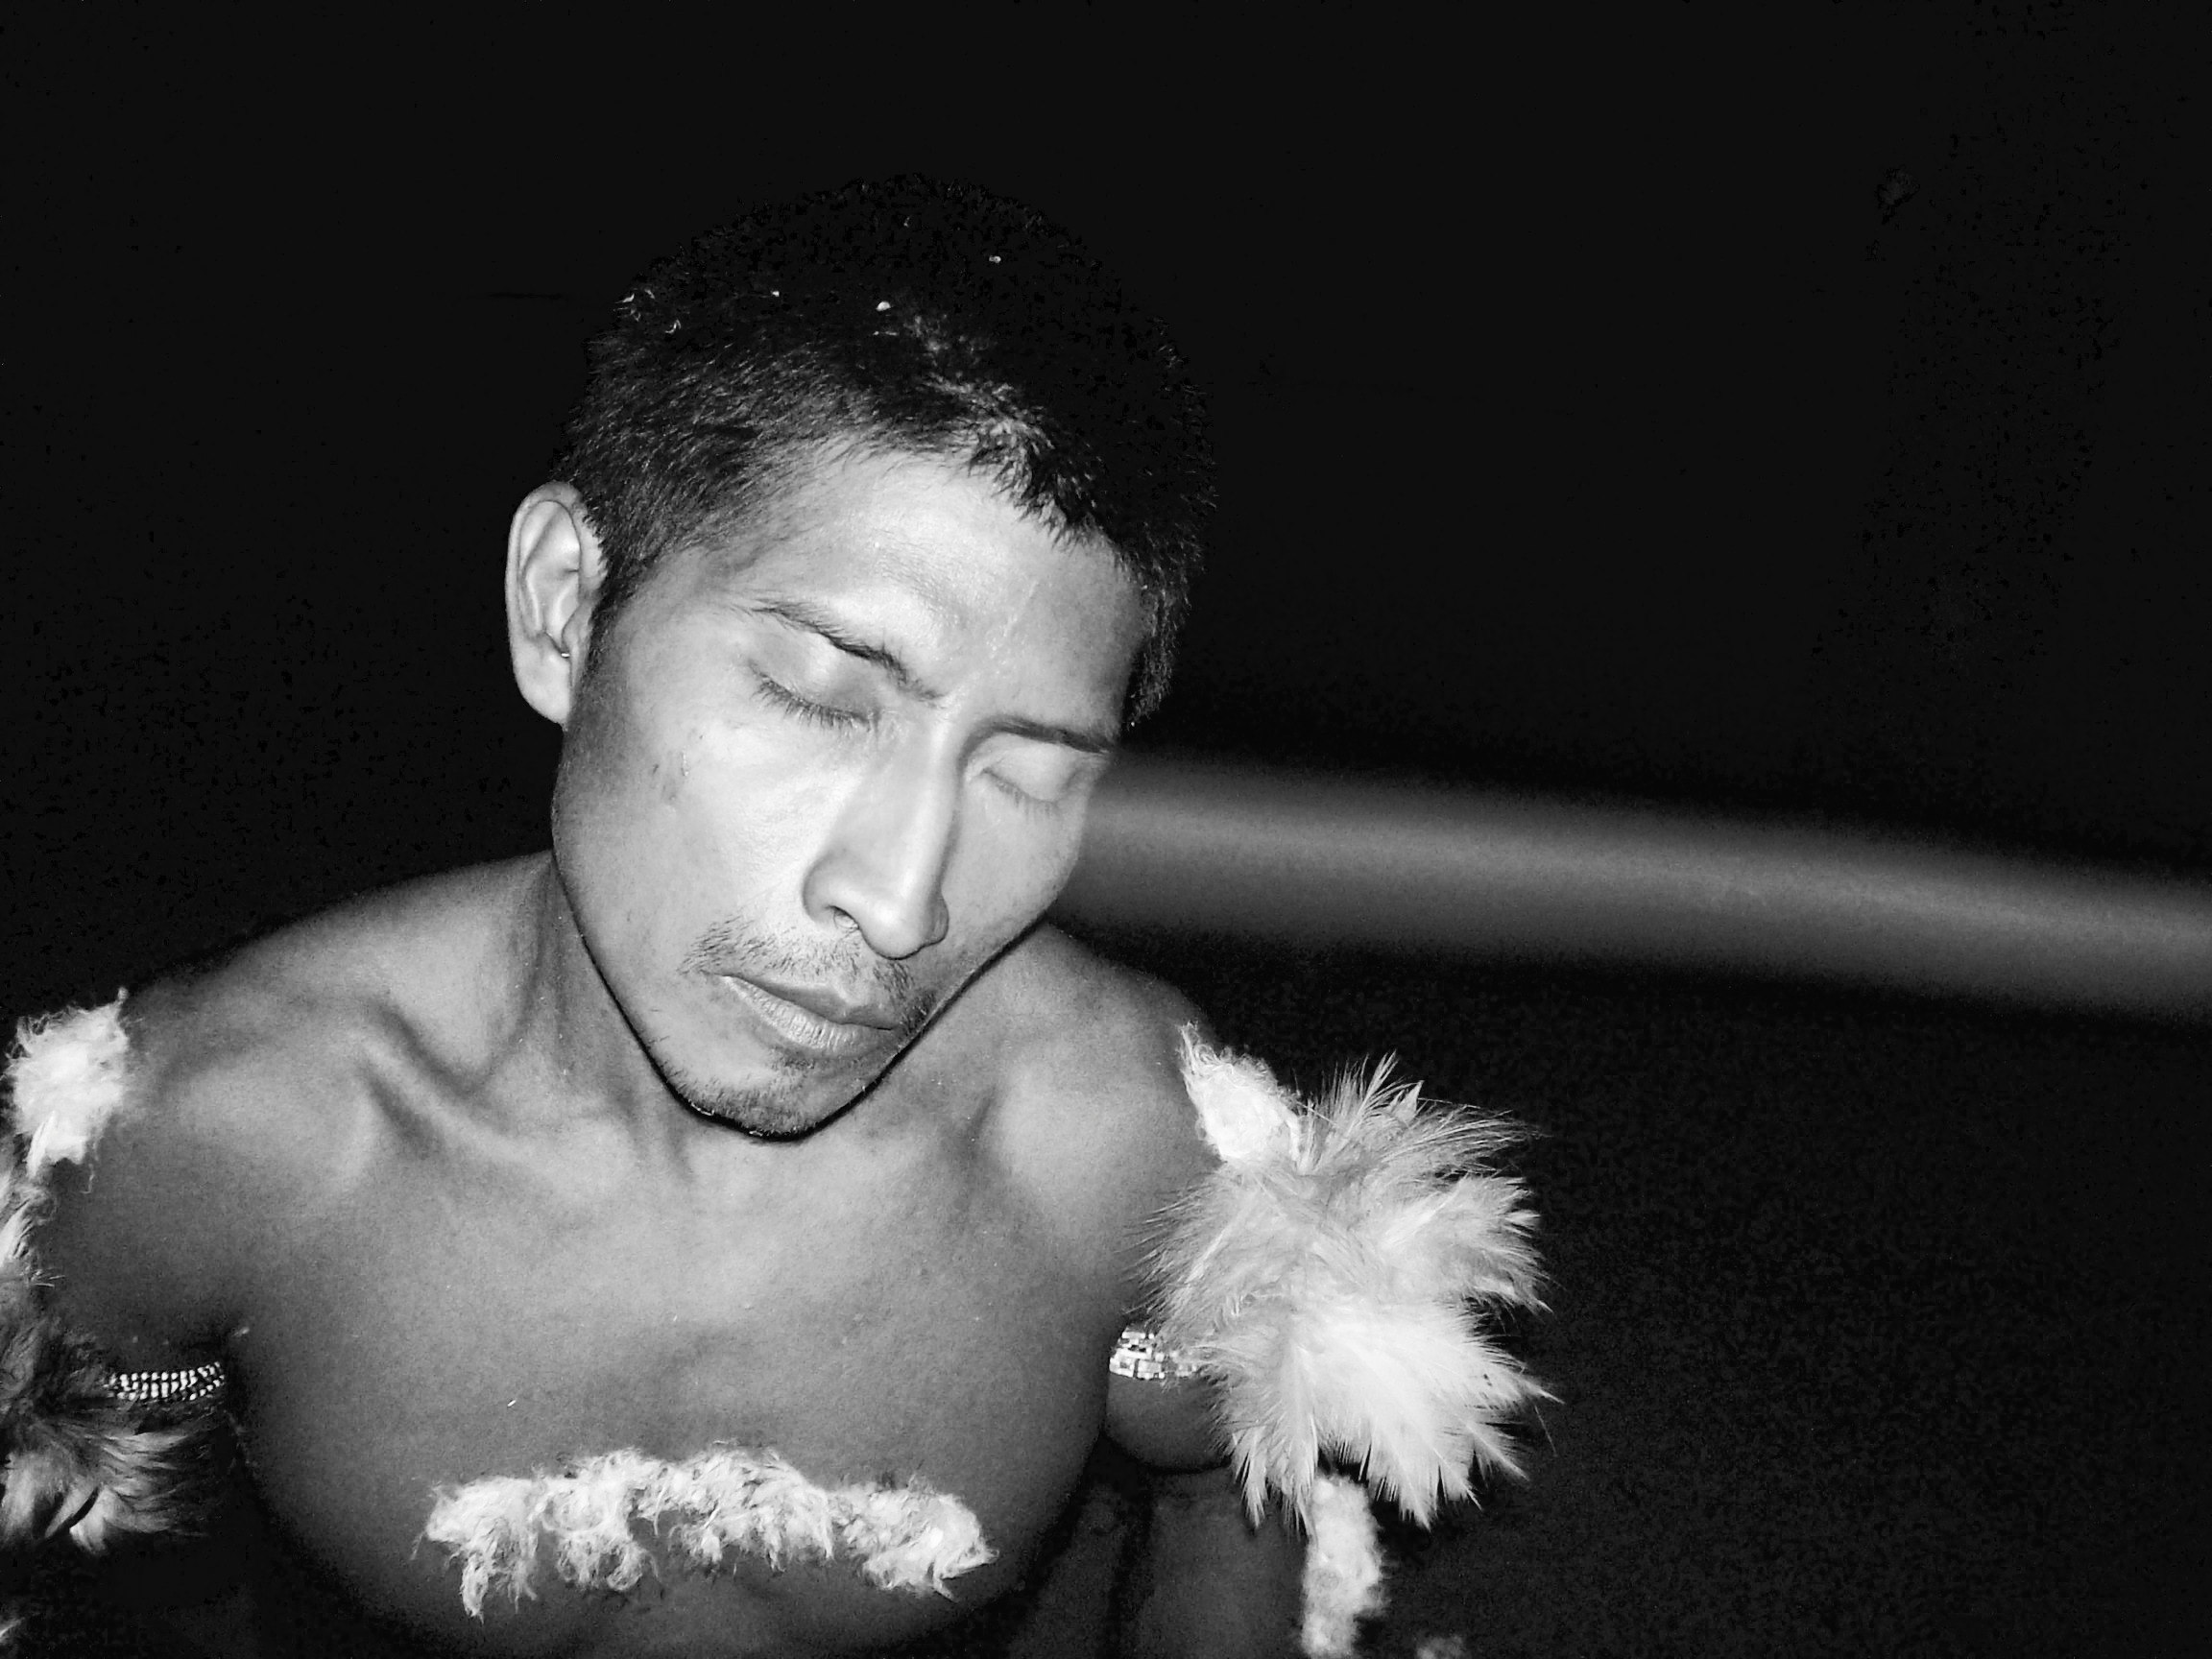
\includegraphics[width=\textwidth]{./imgs/100_1752}
%\caption{Um \textit{karawara} trazido pelo irmão de Wiraho e Hemokoma’a durante a cantoria na \textit{takaja} (aldeia Juriti, 2008).}
%\end{figure}

\epigraph{Se eu morrer, minha pele fica na Terra, as pegadas do meu pé
ficam na Terra. Minha pele torna-se \textit{ajỹ}. Meu coração, minha alma e minha carne vão
para o céu. Ficam vivas. Ficam no céu, tornam-se \textit{karawara}. Ficam cantando,
dançando, transformados em \textit{karawara}. As penas brancas e as vermelhas (que adornam os \textit{karawara}) ficam no céu.}{\textsc{irakatakoa}, aldeia Awá, 2006\footnotemark}

\footnotetext{\textit{Amanõ xi, ikwẽ ha pirera
  wype, ha pyporera wype. Ha pirera iko ajỹ neme. Ha ja'ajna, ha ritekera, ha'okera oho
  iwape. Ikwẽ. Iku iwape, iku karawa neme. Jã ika, panỹ ika, oho karawa neme. Hawiju, japakwa iku iwape}. Coletado e traduzido por Marina Magalhães, 2006.}

\noindent{}Os \textit{karawara}, como mencionado em outras partes do livro, são uma
complexa classe de seres que povoam os patamares celestes e atuam na
Terra de diversas maneiras. São caçadores infalíveis, ao mesmo tempo que
espíritos auxiliares no xamanismo; são o destino de todo ser humano,
\textit{awatea}, após a morte, porém têm uma existência independente,
desvinculada da morte terrena. Os \textit{karawara} são ``gente'',
\textit{awa}, dizem os meus amigos, humanos de verdade, \textit{awatea},
porém uma gente que vive no céu; são relacionados a pequenos mamíferos,
sapos, insetos de todo tipo, plantas, fenômenos naturais, objetos,
plantas cultivadas (como a macaxeira), mas sobretudo a aves. Pombas,
gaviões, rolinhas, beija-flores, pica-paus, socós, juritis, dentre
outros, são gente no céu, e cada \textit{karawara} ganha na Terra um
``correspondente'', que são como suas extensões terrenas. Nos patamares
celestes, \textit{iwa}, se conformam como diferentes tipos de gente como
uma gente pica-pau, gente juriti, gente tucano, papagaio, siricora,
sabiá, várias borboletas, marimbondo, gente-taquara, dentre outras
plantas e bichos, também referidos como \textit{jara}. Por serem exímios
caçadores e embora vivam no céu, \textit{iwa}, mantêm um trânsito
constante com a Terra, para onde descem a fim de buscar, basicamente,
caça, água, mel e, por vezes, fogo, produtos essenciais ao desenrolar da
vida celeste. Têm uma imagem humana celestial definida: bem adornados
com cocares e braceletes, habitantes de um lugar limpo e agradável,
caçadores infalíveis, cantores magníficos e falantes de uma outra
língua, uma fala celeste --- \textit{iwa ma'iha}, ``fala do céu'' --- cuja
prosódia é o canto, \textit{jãnaha}. Uma gente celeste cujas carcaças
animais --- as ``pegadas'', \textit{ipopokera} --- seriam suas formas terrenas.
Em poucas palavras, seriam \textit{eles}, ao mesmo tempo, caçadores e
xamãs magníficos.

Ao descerem à Terra (para caçar, extrair mel ou buscar água), os humanos
não os encontram, pois, além de serem rápidos em suas caçadas (como
veremos adiante), as realizam em locais e matas distantes, onde os Guajá
não alcançam. Se perguntarmos a uma pessoa das aldeias Jurití, Awá ou
Tiracambu sobre ``o que é'' um \textit{karawara}, provavelmente teremos
respostas como: \textit{awa} \textit{parãhy}, ``são humanos belos''; ou
\textit{awaete}, ``são gente de verdade''; ou \textit{awa} \textit{katy}, ``são
pessoas boas''; ou ainda, \textit{karawara} \textit{wate}, ``os
\textit{karawara} estão lá em cima''. E mesmo em português, quando queriam
me fazer entender, falavam ``\textit{mesminho eu, mesminho eu!}'', algo como
``são exatamente como nós somos!'' Além disso, os \textit{karawara} são
sempre referidos como ``\textit{parentes}'' (quando falam em português), uma
ideia que englobaria todas as acima. Ao mesmo tempo, como veremos, os
\textit{karawara}, mais do que ``entidades celestes'', são princípios de
ação (xamânica e cinegética) que desafiam a lógica de nosso entendimento
metafísico, não podendo ser enquadrados apenas como seres (ou
substâncias) ou apenas como fazeres (ou procedimentos). No decorrer do
livro já mencionei os \textit{karawara} algumas vezes, porém neste
capítulo gostaria de apresentá-los mais detalhadamente e buscar algumas
conexões com o que já escrevi até aqui, principalmente no que se refere
às ideias de \textit{jara}, \textit{nima} e \textit{riku}.

Termos correlatos a \textit{karawara} aparecem na bibliografia etnológica;
vejamos rapidamente alguns casos.

\section{variações tupi}

A ideia do \textit{karowara} é recorrente entre os povos Tupi da Amazônia,
algo como uma ``imagem-espírito antropofágica onipresente'' em diversas
dessas cosmologias (Calheiros, 2014, p.\,265), encontradas tanto em
trabalhos clássicos, como Wagley e Galvão (1961), Nimuendajú (1915),
Ribeiro (1996), passando por Laraia (1986), Viveiros de Castro (1992),
Andrade (1992), Fausto (2001) até trabalhos recentes, como Garcia (2010)
e Calheiros (2014). Por exemplo, entre os Parakanã, \textit{karowara}
aparece como ``uma categoria de espíritos com características canibais,
ligados à produção da doença e associados amiúde ao anhanga, ser
antropofágico das cosmologias tupis''. Entre este povo, o \textit{karowara}
atua como um princípio canibal que deve ser domesticado pelos curadores
(Fausto, 2001, pp.\,338--339). Esses agentes-objetos são passados a um
homem por meio de um sonho com o ``senhor dos \textit{karowara}'' ou
``arrancador de \textit{karowara}'', e quando isso ocorre é sinal de que o
sonhador tem grande propensão para a feitiçaria. Aos feiticeiros, os
\textit{karowara} são ``transmitidos'' em sonho e absorvidos pela boca, que
os faz ter ``o gosto-odor de sangue na boca''. Ao lado dos
\textit{topiwara}, os \textit{karowara}, formam um grupo de espíritos,
\textit{karowara}, e objetos, \textit{topiwara}, patogênicos que introduzem
doenças no corpo de alguém; e só os homens que os controlam os podem
retirar. A diferença entre \textit{karowara} e \textit{topiwara} é
estabelecida pelo nível de domesticação de cada um, embora ambos sejam
controlados pelos xamãs e utilizados em suas curas; somente os
\textit{topiwara} são ``xerimbabos bem domesticados'', quase ``filhos
adotivos'' daquelas pessoas que têm poder xamânico (Fausto, 2001, pp.
339--340).

Para os Akuáwa Asurini (os Asurini do Tocantins), Andrade define os
\textit{karowara} como ``substâncias-forças'' cujo controle constitui a
principal característica do xamanismo desse povo, já que os
\textit{karowara} são a ``fonte do poder do pajé'' (Andrade, 1992, p.\,84).
De maneira geral, são forças potentes que podem atacar os humanos
lançando-lhes doenças e que devem ser controladas pelo pajé ou ainda por
outros homens que o saibam fazer. O \textit{karowara} dos Akuáwa Asurini
também pode penetrar no corpo dos humanos, quando atirado por um
espírito chamado \textit{takwitimasa}, dessa vez, provocando-lhes doenças.
Tais seres (que podem assumir a forma de uma abelha ou a forma humana),
quando lançam \textit{karowara} nos humanos, se aparentam como homens
baixos, da estatura de uma criança de nove, 10 anos (Andrade, \textit{op.\,cit.},
p.\,128.) --- exatamente como os Guajá definem os \textit{ajỹ} (tal como
vimos no capítulo 3).

Tanto os \textit{karowara} atirados na mata pelos \textit{takwitimasa} dos
Akuáwa Asurini quanto os ``agentes patogênicos'' notados por Fausto entre
os Parakanã estariam próximos àquilo que os Guajá denominam
\textit{ha'aera}, a ``raiva'' (um agente patogênico), lançada por animais ou
\textit{ajỹ} aos humanos que caminhem na floresta, e outras situações,
como já vimos. Originalmente, os Guajá afirmam que o \textit{ha'aera} é o
\textit{karawara} desses animais e dos \textit{ajỹ}. Enquanto os homens,
esses fazem suas curas com a ajuda dos \textit{karawara}, manipulando o
``ar celeste'' a partir desse princípio (como veremos a seguir); as
doenças lançadas aos humanos por esses inimigos da floresta, na forma de
\textit{ha'aera}, são vistas (do ponto de vista desses animais inimigos)
de maneira semelhante à qual os homens enxergam os \textit{karawara}, isto
é, um fundamento de cura. Os Guajá, ao adoentarem devido a ataques de
fantasmas ou por vingança animal, diferentemente do que ocorre com os
Asurini, não afirmam ser esse um ataque de \textit{karawara}, mas sim,
como já vimos, do \textit{ha'aera} de determinado ser. Um ``\textit{karawara}
reverso'', pois só o é da perspectiva de quem o lançou, seja um animal ou
um \textit{ajỹ}).

Segundo Müller, para os Asuriní do Xingú \textit{karovara} são xamãs
míticos que outrora viveram na Terra e que, desde a separação dos
mundos, habitam o patamar celeste. Eles descem à Terra durante o ritual
do \textit{maraká} e se instalam na casa onde ocorre a cerimônia. Os
Asurini mencionam três tipos deles: os \textit{karovara} do céu,
\textit{karovara} da água e \textit{karovara} de \textit{tivá}, que vivem nos
rios e florestas. Além de participarem dos rituais, os \textit{karovara}
também podem lançar doenças nos humanos, caso esses últimos ignorem
certos cuidados, como por exemplo ``pronunciar o nome de \textit{karovara},
próximo à água: o \textit{karovara} entra no corpo da pessoa, corta-o por
dentro, provocando vômito e defecção de sangue'' {[}\ldots{}{]} (Müller, 1993, p.
169). A doença por \textit{karovara} é uma das muitas que pode acometer um
humano e é extraída por um procedimento chamado \textit{petymbô},
instituído durante o ritual do \textit{maraká}.\footnote{Ver Müller, 1993, pp.
168--174.} Por outro lado, os \textit{karovara}, por serem xamãs
primordiais, auxiliam os xamãs Asurini em suas curas, fornecendo-lhes
\textit{ynga}, ``princípio vital'', que será transmitido aos pacientes na cura
de doenças (Müller, 1993, pp.\,169--170). Os \textit{karovara} dos Asurini
vivem no patamar celeste e de alguma maneira (ao lado dos seres chamados
\textit{tivá} e os \textit{apykwara}) reproduzem a humanidade nesse outro
mundo.

Em um trabalho recente, Calheiros discute etnograficamente o tema
trazendo novos elementos a partir dos Aikewara, em que sofistica
proposições como a de Laraia, que defendia, como uma de suas duas
hipóteses, os \textit{karovara} como seres que vivem nas grutas, entidades
ligadas diretamente ao xamanismo (Laraia, 1986, p.\,239). No caso
Aikewara, a partir da etimologia da palavra, Calheiros propõe uma
definição mínima para \textit{karuwara} como ``aquele que come'', tal o
verbo \textit{karu}, ``comer'', amplamente difundido em línguas
tupi-guarani (Dooley, 1982) e que no caso Guajá aparece como \textit{'u}
(\textit{u'u} na forma lexicalizada). De acordo com o autor, trata-se de
``um povo de seres-espíritos, caçadores magníficos que, hoje, vivem em
uma aldeia encravada nas rochas do alto da Serra das Andorinhas''
(Calheiros, 2014, p.\,266), um povo de gigantes que ostentam corpos nus e
pintados, adornados por um estojo peniano e diademas com penas de gavião
real:\footnote{\textit{Idem}.}

\begin{quote}
O ponto é importante para os Aikewara, eles (os \textit{karuwara}) não
são ``aqueles que se foram'', eles não são seus mortos, seus ancestrais,
eles são outros, são seus inimigos, falam, inclusive, uma outra língua,
incompreensível aos ouvidos de um Aikewara médio, uma língua que somente
os \textit{se'engara'e} dominam. E mesmo que pudessem despi-los de suas
pinturas, mesmo que falassem sua língua, os Aikewara não os
reconheceriam como semelhantes {[}\ldots{}{]}.\footnote{Calheiros, \textit{op.\,cit.}, p.\,266.}
\end{quote}

Dentre as formas aqui apresentadas, encontramos um ar de família entre
os \textit{karuwara} Aikewara e \textit{karovara} Asurini em relação aos
\textit{karawara} Guajá, como continuaremos vendo, com a ressalva de que,
no caso dos Guajá e diferentemente dos Aikewara, virar esses ``outros''
é o destino de todo ser vivente.

De certa maneira, a partir desses breves exemplos podemos afirmar que a
literatura etnológica, a depender do contexto etnográfico, sempre
apresentou a ideia do \textit{karowara} (para utilizarmos a notação de
Laraia) a partir de duas definições. Ora, associados ao \textit{feitiço} e
\textit{agentes patogênicos} nocivos à saúde humana, causadores de doença;
ora, associados a entidades do tipo ``xamãs míticos'', especialista em
cura e de uma vida celeste magnífica, tal como o caso Asurini do Xingu,
ou ainda como seres necrófagos que enxergam a humanidade como animais
dos quais costumam se alimentar, tal o caso Aikewara. Entre os Guajá,
como veremos agora, tal ideia aparece bastante transformada, pois os
\textit{karawara} são, sim, seres-espíritos, muitos dos quais perigosos à
humanidade, ao passo que outros tantos são auxiliares dos humanos em
ações de cura, o mesmo tempo que possuem uma existência como entidades
do tipo ``xamãs míticos'', definindo o que de mais próximo seria algo como
o ``xamanismo'' nesse lugar, uma vez que aqui também estamos diante de
mais um desses povos com \textit{xamanismo} e sem \textit{xamãs}, se assim é
possível colocar (Lima, 1995, p.\,151; Pedersen, 2011). Esses seres
\textit{são} \textit{karawara} e \textit{fazem} \textit{karawara}, como veremos
agora.

\section{pegadas no caminho}

Os \textit{karawara} são caçadores! --- \textit{watama'a}, ``caminhadores''.
Como me lembrou, certa vez, Tatuxa'a: ``são caçadores bons mesmo''! Cada
um desses seres-espíritos é especializado em um tipo de caça ou
atividade, como o \textit{karawara} \textit{Pu'uwa jara}, ``gente
pássaro-carretão'', que é um caçador de macacos-pregos; o \textit{Makaroa},
``gente pomba-galega'', um grande caçador de porcos, cujo canto de caça é
bastante apreciado pelos humanos; o \textit{Xakara jara}, ``gente
gavião-caracoleiro'' e ``gente-gavião-peneira'', um caçador de capelães; o
\textit{Taky jara}, ``gente tucano-de-bico-preto'', que se alimenta de
bacabas; o \textit{Wahaa jara}, ``gente caranguejo-do-rio'', um caçador de
veados; e o \textit{Hajra} \textit{jara}, ``gente irara ou papa-mel'', que
desce à Terra para coletar grande quantidade de mel. Quando as pessoas
encontram uma colmeia seca na floresta, foi \textit{Hajra jara} que desceu
à Terra e coletou o mel, não deixando nada para eles. Cada
\textit{karawara} é ``comedor'', \textit{i'uhara}, de determinado tipo de
alimento: caçam e comem especificamente um único tipo de caça. Como
discutirei aqui, eles têm uma dieta exclusiva, como, por exemplo, as
entidades comedoras \textit{'ã}, encontradas entre os Araweté (Viveiros de
Castro, 1986, p.\,233), que também comem alimentos específicos. Algumas
plantas, como a bacaba e o inajá, também têm uma forma humana celeste,
\textit{karawara}. Por exemplo, \textit{Inaja jara}, ``gente inajá'', é um
grande caçador de capelães, e \textit{jawo'ĩ jara}, ``gente palmeira ubim'', é
um caçador de saguis, \textit{atamari'iia}.

Em relação aos \textit{karawara} há uma correlação entre a ideia de
\textit{jara} e a de ``humanidade celeste'', por assim dizer, por isso opto
por chamá-los de ``gente'' acrescido do tipo correspondente (animal ou
outro) que compõe seu \textit{rastro} na Terra. Mais do que nomes
próprios, os \textit{karawara} são uma multiplicidade --- sempre estaremos
falando em ``\textit{karawaras}'', no plural. Por exemplo \textit{Axu jara},
os \textit{karawara} cujo duplo terreno é uma ave do tipo cuco, conhecida
como ``alma-de-gato'' (\textit{Piaya} \textit{cayana}{]}); são portanto um
tipo de ``gente-pássaro-alma-de-gato'', que provavelmente terá como
chefe, \textit{tamỹ}, um \textit{Axu jara} ``principal'', mas sua família,
sua mulher, seus parentes são todos dessa mesma ``gente'' \textit{Axu
jara}. Basicamente uma gente do céu, \textit{awa iwapahara}, como afirmam
os Guajá, em contraste com eles mesmos, que são \textit{awa wypahara}
(gente da Terra), ou mesmo, como foram durante muito tempo, \textit{awa
ka'apahara}, ``gente da floresta''.

Também estamos vendo aqui que os \textit{karawara} são pensados como
\textit{jara}. Por exemplo, \textit{inaja jara}, para o qual uma tradução
possível seria ``dono dos inajás'', é concebido não em razão do que
supostamente ``criaria'' (frutos de inajá), mas sim quanto ao que
efetivamente caça: capelães, no caso. \textit{Inaja jara}, diferentemente
de um ``dono dos inajás'', aparece como um tipo de gente que habita o céu
(uma multiplicidade: homens, mulheres, crianças), a gente \textit{inaja
jara}, cujo alimento são capelães; e assim será com todos os outros
\textit{karawara}. A ideia de \textit{jara,} nessas circunstâncias, se
aproximaria de outras ameríndias, tal como a noção marubo de
\textit{vaká}, algo como duplos ``cuidadores'' ou ``protetores'' (Cesarino,
2010, p.\,152). Aqui, os correspondentes terrenos (plantas e animais, por
exemplo) não seriam seres de criação de donos celestes, mas verdadeiras
encarnações dessas potências ou, nas palavras Guajá, \textit{ipopokera},
isto é, ``pegadas''.\footnote{\textit{Ipopo}, ``rastro'', ``pegada'' mais \textit{kera},
sufixo de atualização nominal retrospectiva).} Na Terra habitada pelos
humanos, \textit{wya}, a maioria dos pássaros, insetos, peixes, alguns
mamíferos, plantas, minerais e mesmo fenômenos naturais (como o vento ou
o trovão) são definidos pela cosmologia \textit{awa} como \textit{pegadas},
\textit{rastros} dos \textit{karawara} no mundo dos humanos. Em outras
palavras, a ecologia aqui é diretamente informada por esses
seres-espíritos; a floresta e os animais são, de diversas formas, os
\textit{karawara} e suas pegadas. O mundo natural se conecta a outro
espaço-tempo (uma vez que os \textit{karawara} são viventes em um tempo e
um mundo algo do passado e algo do porvir) com seres-espíritos atuando
no mundo sob a forma de uma paisagem habitada que, como sugerem diversos
autores, sempre integrará tempo e espaço (Ingold, 2000, p.\,208), e neste
caso específico sugere diversas temporalidades. Uma das hipóteses aqui
sustentada é a de que os \textit{karawara} informam e traduzem a própria
ideia de \textit{ecologia}, para evocar a definição de Davi Kopenawa para
o termo.\footnote{``Desde o início dos tempos, \textit{Omama} (o herói
  criador) tem sido o centro do que os brancos chamam de
  \textit{ecologia}. Isso é verdade! Muito tempo antes destas palavras
  existirem e eles falarem tanto sobre isso, elas já estavam em nós,
  embora não as nomeássemos da mesma maneira. Para os xamãs, estas têm
  sido palavras provenientes dos espíritos para defender a floresta. Se
  nós tivéssemos livros como eles têm, os brancos poderiam ver quão
  antigas estas palavras são! Na floresta, nós, seres humanos, somos a
  ecologia. {[}\ldots{}{]} As palavras da ecologia são nossas palavras antigas,
  dada por \textit{Omama} aos nossos ancestrais no início dos tempos''
  (Kopenawa \& Albert, 2013, p.\,393, livre tradução).} A paisagem como
algo inacabado e em eterna construção, um ``\textit{going on}'', nas
palavras de Ingold (2000, p.\,172), é aqui determinada por uma
\textit{ecologia} que só será entendida se pensarmos em conjunto com o
conceito de \textit{karawara}. Parafraseando Kopenawa, na floresta, os
\textit{karawara} seriam a própria ecologia.

Os pássaros na Terra não seriam animais de criação, mas partes terrenas
de uma versão celeste. ``Rastros terrenos'' dos \textit{karawara,} dizem os
Guajá; a palavra é \textit{ipopokera}, algo como as ``pegadas'' dos
\textit{karawara}. São um tipo de ``gente'', \textit{awa}, antes de tudo,
``parecido comigo'', \textit{a'e rawỹ jahaa}, afirmam os Awá. Além disso os
Guajá estão muito mais preocupados com o que os \textit{karawara} caçam e
comem do que com o que eles supostamente ``criam'', por isso, como
veremos aqui, não os associo a ``donos dos animais''. Por isso o
\textit{karawara} \textit{Tapa'ya} (gente formiga-correição) é um grande
caçador de antas, cuja eficiência na captura do animal é muito superior
à humana. Ele também pode ser chamado de ``comedor de antas'',
\textit{tapi'ii 'uhara}, e seu canto é chamado ``canto do comedor de
antas'', \textit{tapi'ii 'uha janaha}, e não ``canto de Tapa'ya''. A sua
extensão terrena, o seu \textit{nimaa}, ``ser'' ou ``duplo de criação'', é uma
frágil formiga chamada \textit{tapa'ya}, ``formiga-correição'', ao passo que
a versão \textit{karawara} no patamar celeste, \textit{iwa}, não seria o
``dono das antas'', mas sim um tipo de ``dono'' que caça antas.

Vimos no capítulo 6 que a relação \textit{riku} é aquela estabelecida de
forma assimétrica entre um \textit{jara} e um \textit{nima}. Porém, nem
sempre a ideia relacionada a esse verbo deve ser de ``controle'' ou
``domínio'', e a própria tradução que os Guajá dão para o termo, ``criar'',
embora envolva assimetria, não denota necessariamente ``controle'', mas
sim algo como uma proximidade cultural (em um sentido amplo). Da mesma
maneira, os polos dessa relação --- \textit{jara} e \textit{nima} --- podem sofrer
traduções que não sejam obrigatoriamente ``dono'', ``mestre'' (de um lado) e
``criatura'' (de outro), embora tais acepções também estejam presentes com
os Guajá, mas não sempre. Seres terrenos que têm versões celestes ou, ao
contrário, seres celestes que tenham versões terrenas são ditos
\textit{jara} de suas versões, \textit{nima}, terrenas, suas ``pegadas'',
porém nessa relação não há controle, apenas uma associação (chamemos)
consubstancial. Os \textit{karawara}, como consubstanciais humanos
(celestes) de diversos seres que conhecemos na Terra e que aqui podem
ser considerados ``duplos'', são concebidos, portanto, como \textit{jara}
desses \textit{nima} terrenos, suas ``pegadas''. Se por um lado podemos
simplificar e afirmar com isso que, para os Guajá, os \textit{donos} estão
no céu, as pessoas não pensam esses sujeitos-espíritos como seres do
tipo ``donos'' (controladores). Eles estariam mais próximos a parentes
distantes, \textit{harapihianã}, ``são \textit{parentes}!'', como sempre me
falavam em português.

É importante relembrar que a relação entre um duplo celeste, 
\textit{jara}, e seu \textit{nima} terreno não implica necessariamente uma
relação de controle. Lembremos também que a relação entre um \textit{jara}
e um \textit{nima} é aquela tida por ``parentes próximos'',
\textit{harapihiara}: é assim entre as mulheres e seus animais de
criação;\footnote{Ver Cormier, 2003.} entre os diversos seres no mundo que se
enxergam como \textit{jara} e criam seus \textit{nima} (por exemplo, a
relação entre um capelão e a formiga tucandeira); e é assim também entre
um \textit{karawara} e seu correlato terreno. Mais do que ``super-donos''
(por viverem no céu em uma espécie de ``plenitude cultural''), os
\textit{karawara} seriam correlatos celestes de seres terrenos. São
\textit{potências animais} de uma fauna e flora muito particulares; seus
\textit{nima} são as criaturas mais improváveis que, no céu, alcançam um
estatuto de magnificência humana. Trata-se de uma \textit{fauna} menor,
composta por insetos, borboletas, plantinhas, passarinhos e pequenos
animais, além de palhas de palmeira, folhas e mesmo sementes, que em
suas versões celestes são caçadores infalíveis e guerreiros bravos. Os
principais \textit{karawara} não seriam grandes animais ou animais de
caça, mas, ao contrário, pequenos insetos e passarinhos que na Terra são
aparentemente insignificantes, enquanto que no \textit{iwa} tomam forma e
vivem como grandes caçadores e chefes. Os animais de caça, por sua vez ---
todos os que vimos até o momento, dos macacos aos porcos, dos veados aos
tatus ---, continuam sendo presas, \textit{ma'a}, tanto para os humanos
quanto para os \textit{karawara}.

Assim como os Guajá não fazem uma associação direta entre os nomes, 
\textit{hawirokaha}, e os animais e plantas que os nominam, \textit{nima},
também não correlacionam diretamente os \textit{karawara} e seus animais
correspondentes. Por exemplo, certa vez estávamos ouvindo o canto do
\textit{Makaroa}, ``pomba-galega'', e eu já sabia que no \textit{iwa}, ``céu'', essa
gente \textit{Makaroa} (além de próxima aos \textit{karaia} --- brancos --- do
céu) é formada por magníficos caçadores de porcos. Porém, quando
questionei a um homem se a pomba-galega que ouvíamos cantar era o
\textit{nima} do \textit{Makaroa} que vivia \textit{wate}, ``no alto'', ``no
ceú'', ele fez questão de enfatizar que se tratava de coisas diferentes,
\textit{amõa} \textit{makaroa}, ``outro \textit{makaroa}''\textit{!}, É como se
dissesse: ``esse aqui é um \textit{makaroa} diferente do \textit{makaroa}
celeste!'' Eles estariam associados, \textit{riku}, mas não são a mesma
coisa, tampouco exercem controle um sobre o outro, tal como nas relações
``donos'' e ``criaturas''. Em outras palavras, o interesse pelos
\textit{karawara} está no que eles \textit{caçam}, e não no que
\textit{criam}, por isso a ideia de \textit{riku}, como ``criar'', parece
passar longe desta classificação. Embora o \textit{riku} seja uma relação
fundamental e os \textit{karawara} sejam ditos \textit{jara} de seus
correspondentes terrenos, os Guajá não têm nenhuma teoria especial sobre
a relação \textit{riku} (no sentido de ``criar'') para os \textit{karawara} e
seus \textit{nima} terrenos --- diferentemente do que defendem para a
relação conjugal ou para as flechas, como vimos. O mais importante dos
\textit{karawara} são seus cantos, curas e capacidades cinegéticas.

Mesmo sendo todos os \textit{karawara} pensados como \textit{jara}, ``duplos'',
muitos contam com nomes idênticos aos de seus \textit{nima} terrenos;
outros contam com o designador \textit{jara}, enquanto outros ainda são
referidos por nominadores como \textit{xa'a}, ``parente próximos''. Alguns
são mais ``falados'' pelos Guajá do que outros, como o \textit{karawara}
chamado \textit{Makaroa}, que é um dos seres celestes mais lembrados por ser um
exímio caçador de queixadas e falar bem a língua dos brancos.
Fisicamente eles se parecem com os humanos, porém são adornados com
braceletes, \textit{jamakwa}, e pequenos cocares, \textit{jakỹ ita},
confeccionados com as penas de araçari e tucano, \textit{takỹna},
enquanto as mulheres vestem saias trançadas com as mesmas penas. Um
detalhe interessante é que, ao longo dos últimos anos, eu ouvi de
diferentes amigos e interlocutores que os \textit{karawara} têm os cabelos
encaracolados, \textit{jakỹra papanihũ}, como muitos humanos,
\textit{awa}, também os têm. Os homens \textit{karawara} ainda têm
aplicadas as penugens brancas da harpia e/\,ou urubu-rei, em rosto,
pernas, braços, tórax e abdômen. Enquanto os Guajá da Terra se adornam
dessa forma somente para as cantorias na \textit{takaja}, os
\textit{karawara} mantêm-se assim constantemente. Os humanos se consideram
netos, \textit{hamiarua}, dos \textit{karawara}, da mesma forma que são
também netos de \textit{Maira}. Os \textit{karawara} dormem em redes,
\textit{kaha}, trançadas a partir de uma fibra clara, quase branca --- de
que os Guajá da Terra não sabem o nome e que só existiria no \textit{iwa}, 
``céu''. E vivem em tapiris, \textit{tapãja}, construídos a partir de
uma estrutura de madeiras muito clara chamada \textit{ira} \textit{nynỹ},
que também só existem nos patamares celestes, como apresentado no
primeiro capítulo. Como já mencionei em algumas passagens, os \textit{karawara}
são grandes caçadores e coletores de mel e frutos na Terra, enquanto
outros têm funções específicas, como produzir arcos ou casas, tapiris.

Esses seres gostam de cantar tanto quanto de caçar, e caçam tão bem
quanto cantam. São caçadores pois, antes, são ``comedores'', \textit{i'uhara}, 
a caça --- \textit{ma'a}, ``bicho'', ``presa'' --- é sua comida. E
os \textit{karawara} são lembrados (pelo menos pelos Guajá) sobretudo
pelos animais de que se alimentam; o tipo de gente celeste que são
parece menos importante. São especialistas na caça, ou coleta, de
determinado tipo de alimento justamente por adotarem uma dieta
exclusiva. Os \textit{karawara} não são caçadores genéricos, pois não são
consumidores genéricos; seu paladar tolera somente um ou outro alimento.
Por exemplo, os \textit{karawara} chamados \textit{Makaratỹ jara} --- cujos
duplos terrenos seriam pica-paus dos gênero \textit{Dryocopus e
Campephilus} (como o pica-pau-de-banda-branca e o
pica-pau-de-topete-vermelho) e que por isso podem ser descritos como
``gente pica-pau'' (ou um \textit{Dryocopus-Campephilus} similar) --- são
antes referidos como \textit{tatu 'uhara,} ``comedores de tatu-canastra'',
sua dieta exclusiva. A canção desse \textit{karawara} fala justamente
sobre seu gosto por caçar e comer esses mamíferos.

Para eles, a Terra é um local sujo, repleto de podridão, doenças e
perecimento, habitado por criaturas desprezíveis a seus olhos, como os
animais de criação dos brancos, principalmente os cachorros --- cuja
palavra na língua \textit{karawara} é \textit{karory'ỹma}, sinônimo para
``lixo'' ---, além de galinhas, bovinos e porcos domésticos, que fazem da
camada terrestre, \textit{wya}, um local onde não se deve pisar. Por isso
mesmo, toda a atividade de caça terrena dos \textit{karawara} é realizada
sem que pisem em solo terreno --- \textit{wype}, ``na Terra''; caçam de cima
das árvores, \textit{wate ira rehe}, da copa e dos galhos, e de lá matam
suas presas, \textit{ma'a}, para retornarem ao céu. Sempre fizeram assim,
desde a época em que viviam junto aos humanos, \textit{awa}. Os
\textit{karawara} sentem tanta fobia pela sujeira terrena que quando
voltam para sua morada passam um tempo cuspindo no chão --- \textit{jaru},
``cuspir'' ---; liberam a sujeira pela saliva a fim de se purificarem, da
mesma maneira que os Guajá fazem na Terra ao limpar vísceras, lidar com
sangue, carne podre ou qualquer outro odor fétido que impregne seus
corpos. Há inclusive alguns \textit{karawara}, como \textit{Inamẽxa'a}
(gente-pássaro-saurá {[}\textit{Phoenicircus carnifex}{]}) e
\textit{Inamẽtyxa'a} (gente-pássaro-anambé-azul {[}\textit{Cotinga
cayana}{]}), que, apesar de serem comedores de tucano, sequer descem à
Terra, pois a consideram extremamente suja.\footnote{De acordo com os
  Aikewara estudado por Calheiros, os espíritos lá chamados
  \textit{karuwara} também não pisam na Terra: ``Os \textit{karuwara} não
  vivem no mesmo mundo que os \textit{awaeté} segundo os cantores
  aikewara, seus pés sequer tocam o solo da Ywyeté (a Terra) --- por isso
  eles não deixam pegadas (Calheiros, 2014, pp.\,267--268).} Kopenawa também
lembra que os \textit{xapiri}, que povoam o universo Yanomami e andam por
caminhos de luz, também consideram a Terra suja e nunca pisam no solo,
que é repleto de folhas podres (Kopenawa \& Albert, 2013, pp.\,56--63).

Como caçadores, alguns poucos utilizam espingardas; a maioria emprega
arcos e flechas. Tanto a munição das armas quanto as flechas são
constituídas por \textit{tata}, ``energia'', ``fogo'', o que faz com que seus
disparos sejam certeiros, pois um brilho é lançado e o animal morre sem
qualquer ferimento e, principalmente, sem derramar sangue. Os
\textit{karawara} têm pavor de sangue. Depois que a presa é abatida,
amarram suas pernas com embira, \textit{iwira}, levam-na para o
\textit{iwa}, e todo o processo de limpeza, \textit{hape}, e cozimento,
\textit{miihĩ}, da carne é realizado lá no céu. Algumas pessoas também me
disseram que o que é levado aqui da Terra é ``só um pouquinho'', 
\textit{mixika'ĩ}, da carne do animal, e já sem sangue. Como os
\textit{karawara} conseguem carne na quantidade que desejam, nunca a
estocam --- \textit{wapy} \textit{manã}, ``guardar'' --- moqueada em suas casas, tal
como fazem os humanos. Ao contrário, eles comem tudo até que se acabe, e
a cada refeição carregam para suas moradas novas carradas de carne da
Terra e do céu. E da mesma madeira branca, \textit{ira} \textit{nynỹ}, que
só existe nos patamares celestes, constroem os moquéns onde assam suas
comidas --- \textit{karawa nimi'ua}, ``comida de \textit{karawara}''.

No passado, muitos \textit{karawara} subiram ao céu como que desapontados
com a humanidade, ao mesmo tempo que legaram muitas coisas aos humanos:
deram-lhes, por exemplo, o fogo, como fez \textit{Majhu} \textit{Jara}
``gente-jiboia'', ensinaram-lhes a comer carne de queixada, como fez o
\textit{karawara} \textit{Panỹxa'á}, ``gente-borboleta-azul''; e mesmo o jacu
que, no mito, alerta \textit{Majira} e seu irmão \textit{Mukuxa'á}
(gente-gambá, ou mucura) sobre que eles estavam sendo enganados pelas onças,
era um \textit{karawara}, \textit{Jaku} \textit{Jara}, ``gente-jacupemba'',
{[}\textit{Penelope superciliaris}{]}). Nesse tempo o céu era mais baixo,
e lá não havia caça, todos caçavam na Terra. Quando os animais abatidos
chegavam no céu, o sangue que escorria deles, ao cair no chão, virava
caça. Por exemplo, o sangue que escorria dos pedaços de queixada, ao
cair no chão do céu era transformado em queixadas, por um processo em
que os \textit{karawara} cantavam, e os animais saíam correndo pelo
\textit{iwa}, os ``patamares celestes''. Assim ocorreu com todos os animais
de caça, e hoje os \textit{karawara} também têm animais no céu, muitos
caçam no céu. Nos dias atuais, quando descem para caçar esses espíritos
preferem o alto das serras do Tiracambu e da Desordem, pois lá não serão
vistos pelos Guajá.

Uma das principais marcas da relação entre os \textit{karawara} e os
humanos talvez esteja encontrada na onomástica, como já discuti. Todos
os nomes de humanos são nomes do céu --- \textit{iwa rawirokaha}, ``nomes do
céu'', literalmente ---, e os \textit{karawara} emprestam seus nomes para os
humanos. Um rapaz chamado Takwaripinihĩ ganhou, portanto, o nome de uma
``gente taquara'' celeste, também chamada \textit{Takwaripinihĩ}. Por
serem tão próximos e tão distantes, podemos dizer que se mantém uma
ambígua relação cooperação e desprezo. Cooperam ao ajudar na caça,
escolher nomes, ensinar cantos, trazer curas e se relacionar mesmo como
parentes --- e muitos Guajá têm cognatos, parentes muito próximos, tal
como irmãos, entre os \textit{karawara}. Ao mesmo tempo, sobretudo pelos
costumes atuais, os homens Guajá que vão ao céu dizem receber muitas
reprimendas dos \textit{karawara}, seja porque estão saindo muito da
aldeia, porque estão comendo comida de branco, ou porque têm ido menos
ao céu durante as cantorias na \textit{takaja}.

Lembrando esse tempo antigo, sempre referido como \textit{imỹna}, 
``antigo'', diversas são as histórias que colocam os \textit{karawara}
como os primeiros humanos que habitavam a Terra, antes mesmo da
existência dos brancos e dos Guajá, tal como são hoje; e os animais e
toda a sorte de seres povoavam como humanos na floresta. Nessa época
viviam esses seus ``avós'' que, por motivos diferentes, a depender da
história, subiram ao céu e não voltaram mais. \textit{Takwa jara}, ``gente-taquara'', 
por exemplo, é um exímio caçador de antas que há muito
tempo vivia entre o céu e a Terra e tinha muitos amigos humanos. Certa
vez desceu a fim de caçar para uma mulher; sua intenção era mesmo se
casar com ela. Caçou tanto capelães quanto antas, pois é um notável
caçador. O pai da jovem, no entanto, não quis que ela se casasse com
\textit{Takwa jara}, e ele, extremamente aborrecido, virou as costas para
a vida terrena e nunca mais voltou. No caso do \textit{karawara}
\textit{xakara}, ``gente-gavião-peneira'', e ``gente-gavião-caracoleiro'', 
um desentendimento com seu irmão ciumento, que tinha medo que este lhe
roubasse a esposa, fez com que se transformasse em gavião e fosse viver
como gente-gavião-caracoleiro no céu. Muitas foram as situações que
fizeram com que os \textit{karawara} se aborrecessem com os humanos e
desistissem da vida terrena. Vejamos um desses mitos.



\begin{quote}
\textbf{A traição dos xerimbabos}\quad
Antes \textit{Tapa'ya}, ``gente-formiga-correição'', vivia aqui, na mata.
Nessa época os brancos não existiam. \textit{Tapa'ya} morava no chão, na
Terra. Vivia aqui na mata com os \textit{kamara},  ``outros indígenas
não guajá''. Os \textit{kamara} nunca gostaram de gente \textit{awa} (os
próprios Guajá recordam o quanto morreram na mão de diversos
\textit{kamara)}. Ainda assim, \textit{Tapa'ya} era um \textit{awa} que os
\textit{kamara} temiam. \textit{Tapa'ya} vivia com eles, ``andava no mesmo
caminho deles'' e tinha-os como seus seres de criação. Os Guajá dizem
que, \textit{Tapa'ya} é o ``dono dos \textit{kamara}'', \textit{kamara jara}.
Esses \textit{kamara} eram seus cativos, seus seres de criação.

\textit{Tapa'y} estava em busca de uma mulher para casar. Ao sair de sua
casa --- onde criava os \textit{kamara} --- andando pela floresta, escutou
vozes que pareciam ser de uma pequena aldeia, um grupo de pessoas que
também vivia na mata e era \textit{awa}, como ele. Nessa aldeia viviam
muitas mulheres ``novinhas'' com quem ele poderia se casar. Ao se
aproximar deles, propôs caçar para um homem cuja filha era solteira.
Junto com o irmão de sua pretendente, \textit{Tapa'ya} foi caçar e
trouxeram para casa duas antas, partidas e alocadas em grandes
\textit{marakũa} (cestos de carregar nas costas trançados com folhas
frescas). As antas eram bem grandes. Ao chegar em casa dispuseram os
enormes \textit{marakũa}, repletos com pedaços de carne, encostados pela
casa, nas vigas que sustentavam o tapiri (a casa), para que todos vissem
tamanha quantidade de carne de anta tinham conseguido. O caçador dividiu
a carne de modo a satisfazer a família da jovem; ela achou muito bom e
foi se aproximando de \textit{Tapa'ya}. Depois disso, \textit{Tapa'ya}
retornou a sua aldeia onde também moravam seus cativos \textit{kamara},
mas prometeu à mulher e às outras pessoas que voltaria para caçar mais
para eles, afinal, ele queria se casar.

Ao voltar para casa, \textit{Tapa'ya} preferiu não dizer aos \textit{kamara}
onde estivera, afinal eles não gostavam de gente \textit{awa} e poderiam
fazer alguma coisa. Logo o gaviãozinho \textit{tawatoa}, ``falcão-relógio'',
{[}Micrastur semitorquatus{]}, começou a chamar pelos \textit{kamara}:
--- Tóóóói, tóóóói, tóóóói. É importante lembrar que o canto do gavião
\textit{tawatoa} avisa aos caçadores Guajá quando há porcos do mato,
queixadas, por perto. As pessoas quando ouvem seu piar, ``tóóóói,
tóóóói, tóóóói'', sempre esperam encontrar uma vara de queixadas. Os
\textit{kamara}, índios diferentes dos \textit{awa}, criados por
\textit{Tapa'ya} (assim como ocorria com todos os \textit{kamara} da época),
detestavam a gente do tipo \textit{awa}, e quando ouviram o canto do
falcão-relógio, foram informados não sobre queixadas, mas sobre a
presença de gente \textit{awa} por perto. Sua caça seria a gente
\textit{awa}, e não porcos. E o \textit{tawato} chamava pelos \textit{kamara}:
--- tóóóói, tóóóói, tóóóói, ``tem índio aqui!'', dizia \textit{tawató}! E os
\textit{kamará} pensaram: --- Tem índio por aqui mesmo! Eles estão lá no
babaçual, vamos até lá. Enquanto caminhavam, sem avisar a seu dono,
\textit{Tapa'ya} pensou que estivessem indo atrás de queixadas pois também
ouvira o piar do falcão-relógio; porém, ao ver a direção que tomavam os
\textit{kamara}, percebeu que estes iriam encontrar o grupo \textit{awa},
seus amigos e, agora, afins. Então disse: --- O falcão-relógio está dizendo
que os porcos não estão para esse lado, estão para o outro lado, vocês
estão pegando a direção errada. Vocês devem ir por lá, e não por aí.
Voltem e mudem a direção, a caça está para lá! Por temerem
\textit{Tapa'ya}, os \textit{kamara} o enganaram, dizendo: --- Tá bom, eu vou
por aqui mesmo!

Ao se afastarem da casa de \textit{Tapa'ya}, se perguntaram: --- Para onde
nosso dono foi ontem? O que será que tem para lá? Encontraram então o
caminho, a trilha desses \textit{awa} na mata, e seguiram em direção à
pequena aldeia onde viviam. Lá chegando, a cercaram em uma emboscada e
mataram todas as pessoas da aldeia. Na manhã seguinte \textit{Tapa'ya} se
dirigia à aldeia de seus amigos e, no caminho, encontrou um grande
rastro de sangue: É muito sangue!, \textit{Tapa'ya} pensou. --- Será que
minha mulher morreu? Quando chegou à aldeia estavam todos mortos,
furados pelas flechas, e os \textit{kamara} ainda estavam lá.
\textit{Tapa'ya} viu a cena, chorou, chorou, chorou. Chorou muito. E viu
os \textit{kamara} lá sentados. Um \textit{kamara} falou com ele: --- Vamos
voltar juntos para nossa aldeia! \textit{Tapa'ya} já estava muito bravo e
não quis falar com os \textit{kamara}. Apenas perguntou: --- Por que vocês
mataram minha mulher? Essa era a minha mulher! \textit{Tapa'ya} logo parou
de chorar, pegou sua taboca e começou a flechar os \textit{kamara}, seus
seres de criação que, visivelmente, haviam escapado a seu controle. Os
\textit{kamara} morreram junto com aqueles \textit{awa}. Foi uma vingança
imediata de \textit{Tapa'ya}. No meio da carnificina, \textit{Tapa'ya}
encontrou uma menina, ainda no fim da infância, bem novinha, que estava
escondida em uma rede e pensou: --- Essa não morreu não! Nosso herói
pegou-a e levou-a para o céu, onde passaram a viver. Depois desse
episódio \textit{Tapa'ya} ficou no céu, \textit{iwa}, e não voltou mais.\footnote{Narrado por Tatuxa'a, 2013.}
\end{quote}

\textit{Tapa'ya}, ``gente formiga-correição'', vive no céu e continua criando
os \textit{kamara} por lá. Esse \textit{karawara} é temido pelos
\textit{kamara}, e a canção de \textit{tapa'ya} tem versos como: \textit{awata
kamara rapepe}, ``eu ando no caminho dos \textit{kamara}''. A principal
característica desse \textit{karawara}, além do fato de ser um exímio
caçador, ou comedor, de antas --- \textit{tapi'i 'uhara}, ``comedor de antas'' ---, é
o controle que exerce sobre os \textit{kamara}, ``outros indígenas não
\textit{awa}'', que vivem nos patamares superiores. Para \textit{Tapa'ya}, os
\textit{kamara} são como suas ``galinhas'', \textit{xamakaja}, tamanha a
quantidade desses cativos criados.

\subsection{Um falar diferente}

Se os \textit{karawara} são a epítome do caçar, \textit{watama'a}, sua
expressão e modo de comunicação é o canto. Uma das diferenças entre os
\textit{karawara} e os \textit{awa} é o fato de os primeiros falarem uma
língua diferente --- \textit{amõa} \textit{i'ĩha}, ``outra fala'' --- e, em linhas
gerais, enquanto ``humanos'' na língua guajá é \textit{awa}, na língua
celeste --- \textit{iwa} \textit{'ĩha}, ``falar do céu'' --- será \textit{karawara}. De
acordo com os Guajá, a tradução para \textit{karawara} é simplesmente
``humano'', porém em outra língua, uma língua falada pelos \textit{awa}
que estão no céu, e lá, no falar deles, sua autodenominação é
\textit{karawara}. A língua dos \textit{karawara}, uma vez operada pelos
humanos, é um meio de cura de doentes, além de ser ela que conecta os
diferentes mundos, tão enfatizados pela cosmologia guajá. Podemos
simplificar que, apenas da perspectiva humana, o falar dos
\textit{karawara} é a linguagem do xamanismo guajá, pensando-o como um
conjunto de procedimentos de cura e conexões de mundos sensíveis: vivos
e mortos, céu e Terra. Ao mesmo tempo deve ser mais do que isso, ao
menos para os \textit{karawara}, é a sua própria língua.

Assim, o que na língua guajá é chamado \textit{jawaruhua}, ``onça-pintada'',
na língua dos \textit{karawara} se chama \textit{ma'amija rawỹpini}, ou,
como já vimos, enquanto na língua dos humanos da Terra a palavra para
``cachorro'' é \textit{jawara}, a mesma para ``onça'', na língua
\textit{karawara} a palavra é \textit{karory'ỹma}, que pode ser traduzida
por ``lixo'', tamanho o desprezo que os \textit{karawara} têm pelos
animais de criação dos brancos. E aquilo que na língua dos humanos é
chamado \textit{karaia}, ``não indígenas'' ou ``brancos'', os
\textit{karawara} chamam \textit{jawarymỹ}. Por exemplo, os \textit{karawara}
chamados \textit{Makaro Jawyxa'a}, ``gente-pomba-galega'', ou simplesmente
\textit{Makaroa}, são lembrados por falar a língua dos brancos e, como
vimos, no céu os brancos são chamados \textit{jawarymỹ}, em vez de
\textit{karaia}. Em outras palavras, esses \textit{karawara} sabem falar
português, e os Guajá das aldeias se identificam com eles, dizendo:
``nós somos parecidos com \textit{Makaroa}, \textit{a'e rawỹ Makaroa}, pois
nós também vivemos com os brancos e sabemos o jeito deles!''. Tatuxa'a e
Irakatakoa, da aldeia \textit{Awá}, me disseram certa vez: --- \textit{Makaroa}
é um grande caçador de porcos e amigo dos \textit{karaia}, ``brancos''.
\textit{Makaroa} fala a língua dos \textit{karaia} e sabe como funciona o
jeito deles (dos brancos). Da mesma forma que \textit{Makaroa}, os humanos
conhecem bem a língua dos brancos e sabem, por exemplo, como falar com a
Funai, comer arroz e farinha. O fato de eles morarem em aldeias, e não
mais no mato, faz com que sejam também bem próximos dos \textit{karaia} e
encontram no \textit{karawara} \textit{Makaroa} uma metáfora interessante do
que seriam suas próprias vidas. Por isso, os Guajá até hoje não entendem
e ficam furiosos, pois os brancos não percebem como eles estão
modificados e não são mais gente da floresta, \textit{awa ka'apahara}.
Não à toa, \textit{makaroa} é o \textit{karawara} mais falado e mais
cantado, não por ser o mais importante ou algo assim, mas porque os
Guajá que vão ao céu se identificam com ele. O canto desse
\textit{karawara} tem frases como ``nós ficamos perto dos brancos''.
Abaixo, a mesma frase nas variantes linguísticas dos Awá e dos
\textit{karawara} e também em português:

\begin{quote}\parindent=0em
\item\textsc{karawara}\\
Oho \textit{jawaramỹna} pyry!

\item\textsc{guajá}\\
Oho \textit{karai} pyry!

\item\textsc{português}\\
Foram para perto dos \textit{brancos}!
\end{quote}

Os \textit{karawara} têm ``outra boca'', \textit{amõa irua}, como dizem os
Guajá. Em outro exemplo, o canto dos \textit{karawara}, chamado
\textit{Juxa'a}, ``gente espinho-da-palmeira-marajá'', diz:

\begin{quote}\parindent=0em
Eu sou um comedor de capelães da floresta\\
eu sou um comedor.\footnote{No original: ``iraropy tawamỹna me'ehara jaha / me'ehara jaha''}
\end{quote}

A partir desse exemplo podemos ver que, na língua guajá, a palavra
para ``capelão'' é \textit{waria}, enquanto os \textit{karawara} chamam os
mesmos animais de \textit{tawamỹna}. Além disso, a floresta, que
é \textit{ka'a} na língua guajá, é chamada \textit{iraropy} no
falar dos \textit{karawara}. O mesmo para o verbo comer e a palavra
``comedor'': enquanto na língua guajá se diz \textit{i'uhara} ou
\textit{u'uhara} --- ``comedor'', \textit{u`u} é o verbo ---, no léxico dos
\textit{karawara} a mesma palavra aparece com \textit{me'ehara}
 --- \textit{me'e}, o verbo ``comer''. O detalhe mais importante desse falar dos
\textit{karawara} reside no fato dessas palavras serem como ``descrições''
dos animais a partir de uma ou mais característica. Como exemplo, o que
os humanos chamam de ``paca'', \textit{kararuhua}, os \textit{karawara}
chamam de ``caça listrada'', \textit{ma'amijaperemuhũa} --- \textit{ma'amija}
``caça'' mais \textit{peremuhũ}, ``listrada''. Ou enquanto os humanos se
referem ao veado-mateiro por \textit{arapaha}, os \textit{karawara} chamam
esse animal de nomes como \textit{ma'amijarapymukua}, ``caça de pescoço
comprido'' --- \textit{irapya}, ``pescoço'', \textit{imuku}, ``comprido'' ---, 
ou mesmo \textit{ma'amijarapyjaharamãja}, ``caça de pescoço e do olho grande''
--- \textit{irapya}, ``pescoço'', \textit{hajaha}, ``olho'', \textit{hamãj}, ``grande''.
E de forma poética os mesmos \textit{karawara} chamam o capelão
(\textit{wari}, para os Guajá) com nomes como \textit{tawamỹna,} ``o falecido
flecha reta'' ou \textit{irarawyxa'amỹna} ``sangue na flecha'',\footnote{\textit{Ira},
``pau'' mais \textit{hawy}, ``sangue'' mais \textit{xa'a}, ``sufixo de nome próprio'' mais
\textit{mỹna}, ``falecido''.} ou mesmo \textit{irarawaxa'amỹna}, ``o que mora na
árvore'', em livre associação entre os animais e a maneira que devem ser
caçados, primordialmente com flechas, ou por viverem no alto da
floresta. Quanto a nós, não indígenas, chamados \textit{karai} pelos
Guajá, os \textit{karawara} depositam --- assim me parece --- certa dose de
desprezo, chamando-nos \textit{jawaramỹna}, ``cachorro morto''. Quanto aos
cães, que conhecidos como \textit{jawara} pelos humanos, os
\textit{karawara} simplesmente os chamam de \textit{kararo'ỹma}, ``lixo'' ou ``o
que não presta'', tal tradução que me forneceram.

Vejamos abaixo um pequeno inventário com diferenças existentes entre
palavras nas variantes linguísticas \textit{awa} e \textit{karawara}, como
gostam de dizer os Guajá, \textit{awa'pahara hawiro kĩa}: ``as pessoas de
lá (do céu) denominam assim''. Esta relação me foi fornecida por
diversos interlocutores que vivem nas aldeias da \textsc{ti} Caru (dentre eles
Tatuxa'a, Warixa'a, Irakataoa, Petua, Hajkaramakỹ, Maihuxa'a e Akamatỹ).
Seguem na tabela a forma descritiva de alguns nomes.

\pagebreak
\noindent\textbf{Diferenças lexicais entre as variantes terrena, \textit{awa}, e celeste, \textit{karawara}, da língua}

\begin{table}[H]
\centering
%\caption{My caption}
\label{my-label}
\begin{tabular}{|l|l|l|}
\hline
\textbf{Português}    & \textbf{Guajá} & \textit{\textbf{Karawara}} \\ [.5pt]
\hline\hline
cantar (eu canto)                                                       & \textit{ajã}                                                        & \textit{aimyry}                                                                                    \\ \hline
cantoria/\,canção                                                         & \textit{janaha}                                                     & \textit{aimyryraha}                                                                                \\ \hline
comer                                                                   & \textit{u'u}                                                        & \textit{me'e}                                                                                      \\ \hline
comedor                                                                 & \textit{\begin{tabular}[c]{@{}l@{}}\textit{u'uhara}/\\ \textit{i'uhara}\end{tabular}} & \textit{me'ehara}                                                                                  \\ \hline
queixada                                                                & \begin{tabular}[c]{@{}l@{}}\textit{xohoa} ou\\ \textit{xahua}\end{tabular}            & \begin{tabular}[c]{@{}l@{}}\textit{ma'amijamõmuxiri} - \\ ``caça que grunhe e\\ bate o dente''\end{tabular} \\ \hline
\begin{tabular}[c]{@{}l@{}}não indígena\\ (brancos)\end{tabular}        & \textit{karaia}                                                     & \begin{tabular}[c]{@{}l@{}}\textit{jawarymỹ} - \\ ``cachorro morto''\end{tabular}                                                                                  \\ \hline
anta                                                                    & \textit{tapi'ira}                                                   & \textit{ma'amija ramãj}                                                                            \\ \hline
veado-mateiro                                                           & \textit{arapaha}                                                    & \textit{ma'amija rapy}                                                                             \\ \hline
papa-mel                                                                & \textit{hairara}                                                    & \begin{tabular}[c]{@{}l@{}}\textit{ma'amijarawajrara} -\\ ``caça do rabo grande''\end{tabular}              \\ \hline
tamanduá                                                                & \textit{tamanawã}                                                   & \begin{tabular}[c]{@{}l@{}}\textit{ma'amijarawajrara} -\\ ``caça do rabo grande''\end{tabular}              \\ \hline
tucano/\,araçari                                                          & \textit{takỹna}                                                     & \begin{tabular}[c]{@{}l@{}}\textit{iratara} - ``o que fica\\ na árvore''\end{tabular}                       \\ \hline
onça-pintada                                                            & \textit{jawaruhua}                                                  & \begin{tabular}[c]{@{}l@{}}\textit{ma'amijarawỹpinĩa} - \\ ``caça pintada''\end{tabular}                    \\ \hline
gato maracajá                                                           & \textit{jawaraca'ĩa}                                                & \begin{tabular}[c]{@{}l@{}}\textit{ma'amijarawỹpinĩa} - \\ ``caça pintada''\end{tabular}                    \\ \hline
\begin{tabular}[c]{@{}l@{}}madeira/\,pau/\\ tronco de árvore\end{tabular} & \textit{ira}                                                        & \begin{tabular}[c]{@{}l@{}}\textit{iraramãja} - \\ ``árvore grande''\end{tabular}                           \\ \hline
floresta                                                                & \textit{ka'a}                                                       & \begin{tabular}[c]{@{}l@{}}\textit{iraropya} - \\ ``dossel da floresta''\end{tabular}                       \\ \hline
cachorro                                                                & \textit{jawara}                                                     & \begin{tabular}[c]{@{}l@{}}\textit{kararo'ỹma} - ``o que\\ não presta''\end{tabular}                        \\ \hline
\end{tabular}
\end{table}



\begin{table}[H]
\centering
%\caption{My caption}
\label{my-label}
\begin{tabular}{|l|l|l|}
\hline
\begin{tabular}[c]{@{}l@{}}diversos pássaros\\ como jacamim,\\ jacu, inhambu,\\ mutum, dentre\\ outros\end{tabular} & diversos           & \begin{tabular}[c]{@{}l@{}}\textit{irapapoa} - ``pássaro\\ de assa''\end{tabular}                                                                                                                                                 \\ \hline
cotia                                                                                                               & \textit{akwixía}   & \begin{tabular}[c]{@{}l@{}}\textit{ma'amijarikwarajua} - \\ ``caça da pelagem\\ amarela''\end{tabular}                                                                                                                            \\ \hline
paca                                                                                                                & \textit{kararuhua} & \begin{tabular}[c]{@{}l@{}}\textit{ma'amijaperemuhũa} - \\ ``caça listrada''\end{tabular}                                                                                                                                         \\ \hline
macaco capelão                                                                                                      & \textit{waria}     & \begin{tabular}[c]{@{}l@{}}\textit{tawamỹna} - ``o faleci-\\ do flecha reta''\\ \textit{irarawyxa'amỹna} - \\ ``sangue na flecha''\\ \textit{irarawaxa'amỹna} - ``o\\ que mora na árvore''\end{tabular}                                             \\ \hline
cuxiú-preto                                                                                                         & \textit{kwixua}    & \begin{tabular}[c]{@{}l@{}}\textit{ma'amijarawỹjamata} - \\ ``caça que parece \\ barbuda''\\ \textit{ma'amijajamata} - ``ca-\\ ça barbuda''\end{tabular}                                                                                   \\ \hline
meu território                                                                                                      & \textit{harakwaha} & \textit{hapunua}                                                                                                                                                                                                         \\ \hline
tatu                                                                                                                & \textit{tatua}     & \begin{tabular}[c]{@{}l@{}}\textit{ma'amijawykwahara} - \\ ``caça que é do buraco\\ do chão''\\ \textit{ma'amijawykwajaxa'a-}\\ \textit{mỹna} - ``caça que é dona\\ do buraco do chão''\\ \textit{ma'amijajamekera} - \\ ``caça que tem casco''\end{tabular} \\ \hline
mel          & \textit{haira}       & \begin{tabular}[c]{@{}l@{}}\textit{ira'i} - ``pauzinho''\\ \textit{ira'ixa'amỹna} - ``aquilo\\ que morreu no pau''\end{tabular} \\ \hline
jaboti       & \textit{hamixa}      & \begin{tabular}[c]{@{}l@{}}\textit{ma'amijajape} - ``caça\\ com casco''\end{tabular}                                   \\ \hline
minha esposa & \textit{harimirikoa} & \textit{haparowa}                                                                                             \\ \hline
meu filho/\,a  & \textit{hamymyra}    & \textit{haparowa}                                                                                             \\ \hline
\end{tabular}
\end{table}


Alguns animais diferentes têm a mesma denominação na variante dos
\textit{karawara}, como as onças e os gatos maracajá; ou o papa-mel e o
tamanduá, por exemplo. Isso provavelmente ocorre pelo fato dos
\textit{karawara} serem ``comedores exclusivos'', como já mencionado, e um
caçador, por exemplo de tatus como \textit{Maniõxa'a}, ``gente
pássaro\textit{makaripy}'', chama sua caça de ``caça do rabo grande'' do
mesmo jeito que um caçador celeste de papa-mel como o \textit{karawara}
\textit{Merowỹ}, ``gente-mosca'', o faz. Há uma forma usada pelos
\textit{karawara} quando retornam de uma caçada --- de porcos, por exemplo ---
que costumam dizer \textit{ma'amijamõmuxiri ajka, haparowa}, ``eu matei
porcos, esposa!'',\footnote{Enquanto os Guajá chamam esposa de
  \textit{harimirikoa}, os \textit{karawara} falam \textit{haparowa}.} tal
uma sentença que usarão independente de estarem se referindo à esposa ou
não.

Além de lexicalmente distinto, a ``língua'' dos \textit{karawara} se
distingue pela forma dos enunciados, pois os humanos celestes só se
comunicam cantando. Trata-se de um falar-cantar. Enquanto os \textit{awa}
``falam'' --- \textit{i'ĩha}, ``fala'' --- os \textit{karawara} ``cantam''
--- \textit{janaha}, ``canto''. Como me falou certa vez Irakatakoa:
\textit{Janaha pepe!}, literalmente, ``pelo canto'' ou ``por meio do
canto''. No céu ``não se fala'', \textit{ni'ĩri}, só se canta
\textit{janaha pepe}; é ``por meio do canto'' que esses seres-espíritos se
comunicam. É necessário ouvir os cantos para (com ajuda e explicações
dos Guajá) atentar para as diferenças lexicais entre a fala terrena e a
celeste. Muitas vezes meu trabalho de campo era entendido pelos meus
amigos como \textit{awa janaha pyhy}, ``pegar a cantoria humana''. Se a fala
dos \textit{karawara} é cantada, foi só ouvindo os cantos que consegui me
aproximar desse falar. E tais cantos são utilizados para curas e caça,
pois os \textit{karawara} ajudam os humanos nas caçadas também. Por
exemplo, um homem pode cantar o canto do \textit{karawara} \textit{Arapio}
durante a noite. Esse \textit{karawara} é um caçador de veados-mateiros,
um \textit{arapaha} '\textit{uhara}, ``comedor de veados''. Sabendo disso --- e
todos sabem ---, a esposa do cantor, e mais quem ouvir, saberá que no dia
seguinte seu marido irá caçar veados-mateiros. Esse mesmo canto
``propiciatório'' pode ser entoado nas noites de verão quando fazem a
\textit{takaja}, ou ainda ser cantado à noite para uma criança doente,
quando o homem cantor traz o \textit{karawara} à Terra para ajudá-lo em
suas curas. Caça, xamanismo e canto estão diretamente relacionados.

Para observarmos melhor a diferença nos falares \textit{awa} e
\textit{karawara}, vejamos a tradução do canto do \textit{karawara}
\textit{Takwarihuxa'a}, uma gente-taquara, caçadores-comedores de
queixadas\footnote{\textit{Tayassu pecari}.} e veados-mateiros.\footnote{\textit{Mazama
americana}.}

\begin{table}[H]
\footnotesize
\centering
%\caption{My caption}
\label{my-label}
\begin{tabular}{|l|l|l|}
\hline
\multicolumn{1}{|c|}{\textbf{\begin{tabular}[c]{@{}c@{}}Canto original ---\\ Variante dos\\ \textit{karawara}\end{tabular}}} & \multicolumn{1}{c|}{\textbf{\begin{tabular}[c]{@{}c@{}}Como\\ foi explicado ---\\ Variante dos \textit{awa}\end{tabular}}} & \multicolumn{1}{c|}{\textbf{\begin{tabular}[c]{@{}c@{}}Tradução\\ para o português\end{tabular}}}
 \\ [.5pt]
\hline\hline
\textit{\begin{tabular}[c]{@{}l@{}}Hatakwaria ariku\\ jaha\end{tabular}}                                          & \textit{\begin{tabular}[c]{@{}l@{}}Hatakwaria ariku\\ jaha\end{tabular}}                                        & \begin{tabular}[c]{@{}l@{}}Eu estou com, ou crio a\\ minha taquara\end{tabular}                        \\ \hline
\textit{Hakĩa ariku jaha}                                                                                         & \textit{Hakĩa ariku jaha}                                                                                       & \begin{tabular}[c]{@{}l@{}}Eu estou com, ou crio a\\ minha flecha-taboca\end{tabular}                  \\ \hline
\textit{Hatakwaripe \textbf{amẽa}}                                                                                         & \textit{Hatakwaripe \textbf{ajka}}                                                                                       & \begin{tabular}[c]{@{}l@{}}Com a minha taquara\\ eu \textbf{mato}\end{tabular}                              \\ \hline
\textit{Hakipe \textbf{amẽa}}                                                                                              & \textit{Hakipe \textbf{ajka}}                                                                                            & \begin{tabular}[c]{@{}l@{}}Com a minha flecha\\ taboca eu \textbf{mato}\end{tabular}                        \\ \hline
\textit{\begin{tabular}[c]{@{}l@{}}\textbf{Ma'amijamõmuxiri}\\ \textbf{amẽa} hatakwaripe\end{tabular}}                              & \textit{\begin{tabular}[c]{@{}l@{}}\textbf{Xahua ajka}\\ hatakwaripe\end{tabular}}                                       & \begin{tabular}[c]{@{}l@{}}O \textbf{queixada} eu \textbf{mato}\\ com a minha taquara\end{tabular}                   \\ \hline
\textit{\begin{tabular}[c]{@{}l@{}}\textbf{Ma'amijarapy} anỹ \\ \textbf{amẽa} hatakwaripe\end{tabular}}                             & \textit{\begin{tabular}[c]{@{}l@{}}\textbf{Arapahaa} anỹ \\\textbf{ajka} hatakwaripe\end{tabular}}                                & \begin{tabular}[c]{@{}l@{}}O \textbf{veado-mateiro} tam-\\ bém, eu \textbf{mato} com a\\ minha taquara.\end{tabular} \\ \hline
\textit{\begin{tabular}[c]{@{}l@{}}\textbf{Ma'amijarapy amẽa}\\ hatakwaripe\end{tabular}}                                  & \textit{\begin{tabular}[c]{@{}l@{}}\textbf{Arapaha} ajka\\ hatakwaripe\end{tabular}}                                     & \begin{tabular}[c]{@{}l@{}}O \textbf{veado-mateiro} eu\\ mato com a minha\\ taquara\end{tabular}            \\ \hline
\textit{Hakipe \textbf{amẽa}}                                                                                              & \textit{Hakipe \textbf{ajka}}                                                                                            & \begin{tabular}[c]{@{}l@{}}Com a minha flecha\\ taboca eu \textbf{mato}\end{tabular}                        \\ \hline
\end{tabular}
\end{table}

\begin{comment}
\medskip
\begin{paracol}{3}
\parindent=0em
\footnotesize
\textbf{Canto original\\ Variante karawara}\\
\textit{Hatakwaria ariku jaha} \\
\textit{Hakĩa ariku jaha} 

\switchcolumn
\textbf{Como foi\\ explicado Variante awa}\\
\textit{Hatakwaria ariku jaha}\\
\textit{Hakĩa ariku jaha} 


\switchcolumn
\mbox{}\\*
\textbf{Tradução}\\
Eu estou com,\\ ou crio a minha taquara\\
Eu estou com,\\ ou crio a minha flecha-taboca

\end{paracol}
\medskip
\end{comment}

\section{\textit{takwarihuxa'a}, «a gente taquara»}

No que concerne à tradução deste canto, fiz uma aproximação para o
português, mas cumpre observar que, primeiro, curiosamente não me foram
fornecidas palavras para flechas, tabocas e taquaras no léxico
\textit{karawara}; depois, que embora a estrutura gramatical (morfologia e
sintaxe) das versões \textit{karawara} e \textit{awa} sejam as mesmas, as
palavras para ``queixada'', ``veado-mateiro'' e ``matar'' são diferentes.

\medskip
\begin{paracol}{3}
\parindent=0em
\textbf{Português}

Queixada

Veado-mateiro

Matar

\switchcolumn[1]
\textbf{Guajá}

\textit{xahua} (ou \textit{xoho}

\textit{arapaha}

\textit{ika} (\textit{ajka} ``eu mato'')

\switchcolumn[2]
\textbf{Karawara}

\textit{ma'amijamõmuxiri}

\textit{ma'amijarapy}

\textit{mẽa} (\textit{amẽa} ``eu mato'')
\end{paracol}
\medskip

Voltaremos a abordar os cantos mais à frente, quando for discutida a
\textit{takaja}. A melhor maneira de entendermos os \textit{karawara}, no
entanto, é apresentando-os. A lista abaixo, que contém o nome de 111
destes seres, não é fechada --- como quase nada seria ``fechado'' nos mundos
amazônicos ---; reflete o momento histórico e interesses da população
atual. Os seres \textit{karawara} que apresento abaixo são os que mais
foram comentados comigo, e alguns pude conhecer ``pessoalmente'' durante
as noites que participei das cantorias na \textit{takaja}. A lista foi
montada de forma gradual e é resultado das conversas, observações e
principalmente da minha participação direta nas atividades rituais
durante a pesquisa de campo. Infelizmente não tenho como assegurar se a
listagem abaixo é extensa ou pequena, se comparada à diversidade dos
\textit{karawara} que existem nos patamares celestes. Quando me falavam
sobre os \textit{karawara}, gostavam de dizer: ``É muita gente!''; e
coisas como ``tem mais gente no céu do que em São Paulo'', para que eu
dimensionasse o tamanho do problema. Se os \textit{karawara} são muitos, é
porque a variedade de seres anda junto com uma grande quantidade de cada
um desses espíritos ou, como preferem os Guajá, essa ``gente'' celeste.
Kopenawa observa que há tantos marimbondos na Terra quanto imagens
(espíritos \textit{xapiri}) deles (Kopenawa \& Albert, 2013, p.\,20). Tal
ideia também deve ajudar a dimensionar o caso Guajá, pois provavelmente
existam tantos beija-flores balança-rabo-de-bico-torto (\textit{Glaucis
hirsutus}), chamados \textit{manimya}, quanto karawara desses
beija-flores. Os \textit{karawara}, assim como os xapiri, parecem ser essa
``multiplicidade de imagens similares'' (Kopenawa \& Albert, 2013, p.\,61),
incontáveis.

Se o \textit{iwa} é um local hiper povoado por uma multiplicidade de seres
\textit{karawara}, os que apresento abaixo se referem a uma pequena
amostragem desse todo; porém são esses os \textit{karawara} mais presentes
na vida dos humanos, como pude perceber e como os próprios Guajá
mencionam. Como os \textit{karawara} são muitos, e por isso passíveis de
diferentes recortes\footnote{Podem ser caçadores ou não caçadores; descem à
Terra ou nunca descem; perigosos ou mansos; dentre outras diferenciações.} a maioria
dos que me foram mencionados são aqueles que frequentam a Terra, 
\textit{wya}, e nela caçam, coletam ou descem para cantar e curar durante
o momento ritual da \textit{takaja}. Quanto à lista apresentada, ressalto
que: 

\begin{enumerate}

\item Transcrevo os nomes dos seres em letras maiúsculas, pois os
trato como nomes próprios
\item Doravante, quando me referir a
\textit{nima} na listagem que segue, a tradução que o leitor deve fazer é
``duplo'', ``pegadas'', \textit{ipopokera}, e não, ``ser de
criação'', como sugeri em outras passagens
\item Embora trate cada espécie
de \textit{karawara} no singular, lembro que existem muitos de cada tipo
\item Em negrito destaco o nome do \textit{karawara} e o seu correspondente
animal em português, possibilitando que se faça uma associação direta
\item Quanto aos pássaros, eles foram identificados a partir do \textit{Guia
de campo de aves da amazônia brasileira}, 2008, de Tomas Sigrist
\end{enumerate}

As informações foram coletadas com pessoas diferentes, em três aldeias,
ao longo de 9 anos de pesquisa; a listagem, portanto, não se pretende
definitiva, é uma apresentação apenas parcial.

Eis os \textit{karawara}:


  \paragraph{\textsc{makaro jawyxa'a} (ou \textsc{makaroa})} ``gente pomba-galega''. Trata-se de uma
  gente \textit{karawara} cujo canto é muito apreciado pelos humanos, \textit{awa}. 
  Ele é um grande caçador de porcos e o faz com o auxílio
  de sua espingarda, \textit{maka}, cujos cartuchos são dotados de
  \textit{tata}, ``energia''. Seu \textit{nima} terreno é o pássaro
  \textit{makaroa} --- \textit{pomba-galega}, \textit{Patagioenas cayennesis}.
  \textit{Makaroa} é muito lembrado por ser amigo dos \textit{karaia}, não
  indígenas, do céu. Fala sua língua, e sua esposa é uma mulher branca.

  \paragraph{\textsc{takwa jara}} ``gente taquara''. É um comedor de antas.
  Trata-se de um dos \textit{karawara} mais lembrados, pois tentou viver
  como humano. Certa vez desceu à Terra para caçar. Sua intenção era se
  casar com uma mulher humana, caçar para ela. Em sua epopeia, caçava
  antas e capelães para uma moça solteira comer. O pai da moça não quis
  que ela se casasse, e o \textit{karawara} voltou para o céu ressentido
  com a humanidade.

  \paragraph{\textsc{pu'uwa jara}} ``gente pássaro-carretão''.
  \textit{Karawara} muito importante por ser praticamente um epíteto do
  caçador de capelães. Seu canto é o mais lembrado durante uma caçada de
  capelães, por exemplo. Sempre que o assunto são os bugios,
  \textit{Pu'uwa Jara} é lembrado de alguma forma. Sua flecha é
  pequenina, do tamanho de ``canetas'', e sua técnica de caça com tais
  ``flechinhas'' é única no mundo. Outro detalhe desse \textit{karawara} é
  que ele é inimigo dos \textit{kamara}, ``outros indígenas'', celestes. Seu
  \textit{nima} terreno é o pássaro \textit{pu'uwaky}, \textit{carretão}
  (\textit{Compsothraupis loricata}).

  \paragraph{\textsc{takwariroxa'a}} ``gente folha da taquara''. Além de
  caçar porcos e tamanduás com suas flechas de taquara, \textit{wy'ya},
  ele abre caminhos, \textit{pea}, do céu à Terra para que outros
  \textit{karawara} venham buscar água. \textit{\textit{Takwariroxa'a}} sabe
  fazer um ``caminho firme'', \textit{pe} \textit{hatỹ}, ``como cimento'', me
  disseram certa vez. \textit{\textit{Takwariroxa'a}} é o próprio
  crepúsculo. As marcas vermelhas que eventualmente aparecem no céu
  durante o pôr-do-sol são a trilha feita por
  \textit{Takwariroxa'a}, e é por ela que os \textit{karawara}
  passam levando água da Terra para os patamares celestes. O duplo
  terrestre desse \textit{karawara} são as folhas de uma taquara chamada
  \textit{takwari ruy}.

  \paragraph{\textsc{japu jara}} ``gente japu''. Como vimos no mito
  que explica a criação-separação entre os mundos, os humanos pediram ao
  pássaro \textit{japua}, japu --- humano naquela época ---, que distanciasse
  o céu da Terra, o que deu origem à atual cosmografia. Até hoje
  \textit{Japu} \textit{Jara} controla os patamares
  celestes, \textit{iwa}, mantendo-os em distâncias seguras uns dos
  outros para que não se afastem nem se aproximem muito da Terra. Além
  disso esse \textit{karawara} caça jabotis na Terra. No \textit{iwa}, sua
  esposa tem capelães como animais de criação. Ele é, junto como o
  \textit{karawara} chamado \textit{japini'i jara}, o responsável por fazer
  os tapiris do céu. Isso se explica em parte, pois seu \textit{nima} na
  Terra é o pássaro \textit{japua} --- \textit{Japu}, \textit{Psarocolius
  decumanus} ---, famoso por construir nas árvores grandes ninhos pendentes
  que mais parecem grandes bolsas.

  \paragraph{\textsc{majhu jara}} ``gente jiboia''. Trata-se da
  \textit{jiboia}, \textit{majhua}, celeste. No céu, ele tem a aparência
  de um \textit{karawara}, mas ao descer para caçar se transforma em
  jiboia e come animais como o veado, cotia e até mesmo porcos. Quando
  ainda vivia na Terra, \textit{wya}, junto com os humanos,
  \textit{Maihu Jara} foi o responsável por roubar o fogo dos
  urubus e passá-lo à humanidade\footnote{Ver anexo de mitos.} Sempre que os
  Guajá da Terra matam uma jiboia, sabem que não se trata de
  \textit{Maihu Jara}, pois esse \textit{karawara} caça em outras
  matas, distante dos humanos.

  \paragraph{\textsc{kaapapanyxa'a}} ``gente marimbondo-caba''. Um grande
  caçador de queixadas e antas. Esse \textit{karawara} tem os
  \textit{kamara} (outros indígenas como os \textit{Tenetehara}) que vivem
  no \textit{iwa} como animais de criação, xerimbabos.
  \textit{Kaapapanyxa'a} mantém os \textit{kamara} presos pelo
  pescoço, em cordas, amarrados em árvores perto de sua casa. É um
  \textit{karawara} muito bravo. Seu duplo na Terra é também uma espécie
  de \textit{marimbondo-caba}, \textit{kaa}.

  \paragraph{\textsc{jamukuni jara}} ``gente gavião-de-penacho''. É um
  caçador de nhambus, macacos-pregos e mutuns. Seu duplo é o gavião
  \textit{jamukunia}, gavião-de-penacho (\textit{Spizaetus ornatos}).

  \paragraph{\textsc{piririxa'a}} ``gente pássaro-suiriri''. No céu são
  como chefes, muito agressivos e controladores. Seu duplo na Terra é o
  passarinho \textit{piriria}, suiriri (\textit{Tyrannus melancholicus}).

  \paragraph{\textsc{wy'y jara}} ``gente flecha''. São caçadores de
  capelães. Como sabemos, \textit{Wy'ya} são as flechas feitas
  para matar capelães, e são também os duplos terrenos de
  \textit{Wy'y Jara}.

  \paragraph{\textsc{takỹ̃ jara}} ``gente tucano-de-bico-preto''.
  Alimentam-se de bacabas. Extraem seus alimentos das bacabeiras
  celestes e também descem à Terra para as colher. Seu duplo na Terra é
  um tipo de tucano chamado \textit{takỹna} ---
  \textit{tucano-de-bico-preto}, \textit{Ramphastos} \textit{vitellinus}.

  \paragraph{\textsc{maniõxa'a}} ``gente pássaro\textit{makaripy}''. É um
  \textit{karawara} horticultor que carrega peso e no céu consome farinha
  de macaxeira (só céu só tem farinha branca de macaxeira). É capaz de
  carregar uma anta inteira nas costas, tal como os humanos fazem com os
  queixadas, o animal mais pesado que carregam. As pessoas costumam
  cantar a canção de \textit{Maniõxa'a} na noite anterior ao trabalho de
  roça para que fiquem fortes --- \textit{hatỹ}, ``duros''. \textit{Maniõxa'a}
  se alimenta, além de farinha de macaxeira, de tatu canastra. É um
  caçador de tatu peba e tatu-canastra --- \textit{tatu ikahara}, ``matador de
  tatus''. Seu duplo na Terra é um pássaro que não consegui
  identificar.

  \paragraph{\textsc{kamarajuxu'a}} ``gente \textit{kamara}''. São versões
  celestes dos \textit{Kamara}, `` outros povos indígenas''. São
  grandes guerreiros e têm os \textit{karaia}, os ``não indígenas'', como
  inimigos. \textit{Kamarajuxa'a} é um caçador de antas e veados. Caça com
  auxílio de lanterna no sistema de espera, \textit{matakwa}, e utiliza
  escopeta calibre 12.

  \paragraph{\textsc{mukuxa'a}} ``gente gambá''. É um caçador de antas e
  caça com uma espingarda calibre 28. Seu \textit{nima} é a mucura, ou gambá
  (do gênero \textit{Didelphis}).

  \paragraph{\textsc{itaxa'a}} ``gente pedra'' (também pode ser chamado de
  ``dono da pedra''). Caçadores de anta. Não à toa, a primeira anta,
  criada por \textit{Maira}, foi feita a partir de uma pedra.

  \paragraph{\textsc{wutuxa'a ou wutu jara}} ``gente vento'', ou ``dono do
  vento''. Um \textit{karawara} que é o próprio \textit{vento}, \textit{wutua}. 
  No \textit{iwa} ele é humano e desce à Terra para
  quebrar galhos e mexer nas folhas. O vento que derruba as árvores é o
  canto de \textit{Wutuxa'a}. O que é visto pelos \textit{awa} como vento é
  percebido por \textit{Wutuxa'a} como canto.

  \paragraph{\textsc{amara'yxa'a}} ``gente chuva'' ou, simplesmente, ``dono da
  chuva''. Quando esse \textit{karawara} canta no céu, a chuva cai na
  Terra.

  \paragraph{\textsc{axu jara}} ``gente pássaro-alma-de-gato''. É um
  daqueles \textit{karawara} que não gostam de humanos, \textit{awa}.
  \textit{Axu jara} são feiticeiros que jogam encantamentos, \textit{ma'akwa}, 
  e dor, \textit{hahy kera}, nos humanos. O feitiço é
  realizado basicamente por enterrar objetos das pessoas, como roupas
  velhas e cabelos. Seu \textit{nima} na Terra é o pássaro \textit{axu},
  alma-de-gato (\textit{Piaya cayana}).

  \paragraph{\textsc{kaxa'y}} ``gente pássaro-estalador-do-norte'',
  ``gente pássaro-abre-asa-da-mata''. Também é um \textit{karawara}
  feiticeiro que não gosta dos humanos. Seu \textit{nima} terreno são os
  pássaros estalador-do-norte (\textit{Corytophis torquatus}) e
  abre-asa-da-mata (\textit{Mionectes macconnelli}).

  \paragraph{\textsc{warajuxa'a}} ``gente borboleta''. Um \textit{karawara}
  muito importante, cujo canto é um dos mais apreciados pelos Guajá.
  Alimenta-se de mel que aqui extrai. Seu duplo terrestre é uma espécie
  de \textit{borboleta}, \textit{panỹ}.

  \paragraph{\textsc{waraju}} ``gente borboleta''. Diferente de
  \textit{Warajuxa'a}, esse \textit{karawara} chamado \textit{Waraju} (um é
  variação do outro) é agressivo e mata os \textit{karaia}, os ``não
  indígenas'' dos patamares celestes.

  \paragraph{\textsc{pinawãxa'a}} ``gente bacaba''. São
  caçadores-comedores, de capelães.

  \paragraph{\textsc{jaharoxa'a}} ``gente jussara-açaí''. Caçam e se
  alimentam de saguis.

  \paragraph{\textsc{jakare jara}} ``gente-jacaré''. Caçadores-comedores de paca.

  \paragraph{\textsc{puku jara}} ``gente pomba-trocal''. É um
  coletor-comedor de jabotis. Esse \textit{karawara} sabe cantar canções
  dos brancos, \textit{karai janaha}, ``canto dos brancos''. Seu duplo
  terreno é a ave \textit{pukua}, pomba-trocal (\textit{Patagioenas
  speciosa}).

  \paragraph{\textsc{marajuxa'a}} ``gente fruto-da-palmeira-marajá''. São
  caçadores de macacos-pregos e macacos mão-de-ouro. Seu \textit{nima}
  terreno é o frutinho \textit{marajua}, ``marajá'', próprio do marajazeiro
  (\textit{Bactris maraja}).

  \paragraph{\textsc{juxa'a}} ``gente espinho-da-palmeira-marajá''. São
  caçadores de capelão. Seu \textit{nima} na Terra são os espinhos do
  marajazeiro (\textit{Bactris maraja}).

  \paragraph{\textsc{inamẽxa'a}} ``gente anambé''. Um caçador de tucanos. 
  Esse \textit{karawara} vem à Terra para olhar, \textit{xa}, as esposas e as crianças. Quando um
  homem vai caçar, seu duplo celeste, \textit{nima}, envia
  \textit{Inamẽxa'a} à Terra para vigiar a esposa e os filhos de
  seu \textit{jara} que permaneceram em casa e se certificar de que
  estarão bem e que nenhum homem vá ficar com sua mulher. De certa
  forma, \textit{Inamẽxa'a} são os ``olhos dos marido''
  --- \textit{imeena xakaha}, ``visão do marido'', disseram --- que, quando vai ao
  \textit{iwa} através da \textit{takaja}, conversa com
  \textit{Inamẽxa'a}. Seu \textit{nima} na Terra são os pássaros
  \textit{inamẽ} (dois tipos de \textit{anambé}:
  \textit{anambé-branco-de-bochecha-parda} \textit{Tityra inquisitor}; e
  \textit{anambé-branco-de-rabo-preto}, \textit{Tityra} \textit{cayana}).

  \paragraph{\textsc{inamẽ papa'ỹ̃}} ``gente-pássaro-caneleiro-preto''. São
  \textit{karawara} que criam capelães no céu. Seu duplo na Terra é o
  pássaro \textit{Inamẽ papa'ỹ}, caneleiro-preto (\textit{Pachyramphus
  polychopterus}).

\paragraph{\textsc{tapa'y}} ``gente formiga-correição''. São caçadores de
  anta. ``São como policiais no céu'', me disse certa vez um amigo, pois
  protegem os \textit{awa} \textit{karawara}, ``gente do céu'', dos \textit{karawa
  mihua}, ``gente brava e selvagem do céu''.

  \paragraph{\textsc{araturaxa'a}} ``gente corujinha-do-mato''. Seu duplo
  na Terra é a coruja \textit{arakwari'ia}, corujinha-do-mato
  (\textit{Megascops choliba}).

\paragraph{\textsc{kapitỹ jara}} ``gente gavião-de-cauda-curta''. É um
  caçador-comedor de nhambus --- \textit{iramu} na língua guajá e
  \textit{irapoxikamỹna}, na língua dos \textit{karawara}. Seu duplo na
  Terra é o gavião \textit{kapitỹ}, gavião-de-cauda-curta (\textit{Buteo
  brachyurus}).

\paragraph{\textsc{xakara jara}} ``gente gavião-caracoleiro'' e ``gente
  gavião-peneira''. São caçadores de capelão. Seu \textit{nima} são os
  gaviões do tipo \textit{xakara,} caracoleiro (\textit{Chondrohierax
  uncinatus}) e gavião-peneira (\textit{Elanus leucurus}).

\paragraph{\textsc{panỹxa'a}} ``gente-borboleta-azul''. É um caçador de
  queixadas.

\paragraph{\textsc{jawataraxa'a}} ``gente-lontra'', ``gente ariranha''.
  São caçadores-comedores de jacaré. Seu duplo terreno é o animal
  \textit{jawatara}, lontra ou ariranha (\textit{Pteronura brasiliensis}).

\paragraph{\textsc{makaratỹ jara}} ``gente pica-pau'' (dos gênero
  \textit{Dryocopus e Campephilus}, como o pica-pau-de-banda-branca e o
  pica-pau-de-topete-vermelho). São comedores de tatu, mel e larvas que
  vêm buscar na Terra. Seu \textit{nimá} são essas espécies de
  \textit{pica-pau}.

  \paragraph{\textsc{arira jara}} ``gente morcego''. Caçadores de
  caititus. Seus \textit{nima} terrenos são os \textit{morcegos}
  \textit{arira}.

\paragraph{\textsc{manaky jara}} ``gente poraquê''. É um \textit{karawara}
  que nunca desce à Terra. Ele é famoso por manter centenas de animais
  de criação celestes (macacos, mutuns, jacus, nhambus, dentre outros).
  Seu \textit{nima} terreno é o \textit{poraquê}, \textit{manakya}.

\paragraph{\textsc{pira jara}} ``gente araçari''. É um caçador de
  nhambus. No céu, esse \textit{karawara} cria muitos animais (quatis,
  pacas, macacos diversos), e seu \textit{nima} na Terra é um araçari (do
  gênero \textit{Pteroglossus}) chamado \textit{takynihĩ}.

\paragraph{\textsc{katexa'a}} ``gente uru-corcovado''. Seu duplo terreno
  é o uru-corcovado (\textit{Odontophorus gujanensis}), chamado
  \textit{urua} na língua guajá.

\paragraph{\textsc{watarawyxa'a}} ``gente palha-do-babaçu''. São
  caçadores de porcos queixadas, e seus duplos terrenos são a
  palha, ou folha, da palmeira babaçu (\textit{Orbignya phalerata}).

\paragraph{\textsc{kamixa tuwira}} ``gente jaboti''. \textit{Karawara} caçador de capelão. Seu \textit{nima} terreno é o \textit{jaboti}, \textit{kamixa}.

\paragraph{\textsc{jaxajhu jara}} ``gente capininga''. Tal como o \textit{karawara} ``jaboti'' acima, \textit{Jaxajhu Jara} também é um caçador de capelães.
  Seu \textit{nima} terreno é a tartaruga de água doce \textit{jaxajhua}
  (\textit{capininga}, \textit{Trachemys adiutrix}).

  \paragraph{\textsc{pakwa'ĩ jara}} ``gente (pássaro) rolinha''. \textit{Karawara} caçador de capelães. Seu duplo terreno é o pássaro \textit{Pakwa'ĩa}, um tipo de
  \textit{rolinha}.

  \paragraph{\textsc{jurixu jara}} ``gente juriti''. Um caçador de capelães. Seu duplo
  terreno são os pássaros \textit{jurixua} (três tipos de juriti:
  \textit{juriti-pupu}, \textit{Leptotila verreauxi};
  \textit{juriti-gemedeira}, \textit{Leptotila} \textit{rufaxila}; e
  \textit{juriti-vermelha}, \textit{Geotrygon violacea}).

\paragraph{\textsc{kiripixa'a}} ``gente ubim'' (a palmeira \textit{Geonoma deversa}). É um caçador de saguis, 
\textit{atamari'ia}, tido como o ``chefe do céu''. Seu \textit{nima} na
  Terra é a palmeira \textit{kiripia} (\textit{palmeira} \textit{ubim},
  \textit{Geonoma deversa}).

\paragraph{\textsc{amỹ kiripi}} literalmente, \textit{mamãe kiripi}
  (o \textit{karawara} acima), ela se alimenta de jabotis que outros
  \textit{karawara} lhe fornecem.

\paragraph{\textsc{wy'y pokaxa'a}} um \textit{karawara} caçador de saguis, 
\textit{atamari'ia}. Seu \textit{nima} terreno é um tipo de taquara, \textit{wy'y}, 
mais fininha.

\paragraph{\textsc{amỹxa'a pinihỹ̃}} trata-se de uma mulher que tem
  macacos-cuxiús como animais de criação e se alimenta de capiningas.
  Seu \textit{nima} na Terra é um pássaro que não consegui identificar
  chamado \textit{wamaxĩa}.

\paragraph{\textsc{kirimixixa'a}} um marimbondo que não pica. Esse
  \textit{karawara} caça tatus. O mais importante desse \textit{karawara} é
  o fato de ser ele o responsável por ressuscitar os humanos ao chegarem
  no céu após a morte terrena (veremos a relação entre a morte e os
  \textit{karawara} mais adiante).

\paragraph{\textsc{hajra jara}} ``gente papa-mel''. Trata-se de uma versão celeste do animal chamado \textit{hajrara}, ``papa-mel''. Este \textit{karawara} desce à Terra
  para coletar grandes quantidades de mel.

\paragraph{\textsc{jua'i jara}} um \textit{karawara} cujo duplo terreno é
  um sapo chamado \textit{jua'ia}.

\paragraph{\textsc{wara kakyjỹ̃}} um \textit{karawara} cujo duplo também é um sapo.

\paragraph{\textsc{kara pyrana'i}} ``gente cará''. Ao lado da macaxeira, é o único
  \textit{karawara} cujo duplo é uma planta domesticada, o \textit{cará}, \textit{kara}. Este \textit{karawara} não caça e é próximo aos
  \textit{karaia} celestes.

\paragraph{\textsc{makaxixa'a}} ``gente macaxeira''. Um \textit{karawara} caçador de porcos. Seu \textit{nima} terreno é a \textit{macaxeira}, \textit{makaxia}.

\paragraph{\textsc{jjrahyxa'a}} é um caçador de capelães. Esse
  \textit{karawara} não tem nenhum correspondente terreno; só existe no
  \textit{iwa}.

\paragraph{\textsc{takwari pinuhũxa'a}} um \textit{karawara} caçador de
  antas. Seu \textit{nima} terreno é um tipo de \textit{taquara} escura.

\paragraph{\textsc{wy'yrara}} um caçador de veados. Seu \textit{nima}
  terreno é um tipo de \textit{taquara}, \textit{wy'ya}.

\paragraph{\textsc{takwari}} um \textit{karawara} caçador de antas. Seu
  \textit{nima} terreno é um tipo de taboquinha (finos bambus).

\paragraph{\textsc{jawajuxa'a}} ``gente-raposa''. Um caçador de cotias e
  quatis. Seu \textit{nima} terreno é a \textit{raposa}, ou \textit{cachorro-do-mato} (\textit{Cerdocyon thous}), chamada \textit{jawajua}.

\paragraph{\textsc{waha jara}} ``gente carangueijo-do-rio''. Um \textit{karawara} caçador de veados. Seu \textit{nima} terreno é o \textit{carangueijo-do-rio}, \textit{waha}.

\paragraph{\textsc{irapa jara}} ``gente pau d’arco''. É uma espécie de ``dono do arco'' celeste. \textit{Irapa Jara} faz arcos de caça sem qualquer ferramenta:
  molda-os com as mãos e em seguida distribui aos outros
  \textit{karawara}. Tem a árvore \textit{pau-d'arco} como \textit{nima}
  terrestre.

\paragraph{\textsc{ajruhu jara}} é um \textit{karawara} caçador de porcos.
  Seu duplo terreno é uma espécie de \textit{papagaio}.

\paragraph{\textsc{makaraxa'ĩa}} ``gente picapauzinho-anão''.
  Alimenta-se de mel. Seu \textit{nima} terreno é a ave
  \textit{Makaraxa'ĩa}, picapauzinho-anão (\textit{Veniliornis affinis}).

\paragraph{\textsc{xxapej jara}} ``gente garrinchão''. Um \textit{karawara} caçador de
  macacos-pregos. Seu \textit{nima} terreno é o pássaro \textit{txapej xoxo}
  (garrinchão-pai-avô, \textit{Pheugopedius genibarbis}).

\paragraph{\textsc{hoa'ĩ jara}} ``gente coco de babaçu''. É um caçador de macacos-pregos.
  Seu \textit{nima} terreno é o coco do \textit{babaçu}.

\paragraph{\textsc{inaja jara}} ``gente inajá''. Um \textit{karawara} caçador
  capelães. Seu \textit{nima} terreno é a palmeira inajá, \textit{inajã}.

\paragraph{\textsc{talwarihuxa'a}} um \textit{karawara} caçador de porcos e
  veados mateiros. Seu \textit{nima} terreno é também um tipo de taquara
  ou taboquinha (que não consegui identificar).

\paragraph{\textsc{kakỹ jara}} ``gente gralhão''. É um \textit{karawara} muito bravo, \textit{imahy}, 
que vem à Terra matar os \textit{karaia}. Seu \textit{nima}
  terreno é o pássaro \textit{kakỹa} (\textit{gralhão}, \textit{Ibycter
  americanus}).

\paragraph{\textsc{wiraho jara}} ``gente harpia''. Um caçador de preguiças,
  diversos macacos e capelães. Seu \textit{nima} terreno é o gavião-real
  (\textit{Harpia harpyja}).

\paragraph{\textsc{taperemỹxa'a}} um \textit{karawara} cujo \textit{nima}
  terreno é um \textit{papagaio} chamado \textit{taperemỹ}.

\paragraph{\textsc{japini'i jara}} ``gente xexéu''. Tal como \textit{japu jara}, esse
  \textit{karawara} constrói tapiris para a população celeste. Seu
  \textit{nima} na Terra é o pássaro \textit{japini'ia} (\textit{xexéu},
  \textit{Cacicus} \textit{cela}), famoso por construir seus grandes ninhos
  pendurados nas árvores.

\paragraph{\textsc{pany'ĩa}} ``gente borboleta''. Um \textit{karawara} caçador de porcos. Seu \textit{nima} é uma \textit{borboleta} chamada \textit{paramuhua}.

\paragraph{\textsc{kiripo jara}} um caçador de jabutis. Não consegui
  identificar seu \textit{nima} terreno.

\paragraph{\textsc{hako jara}} ``gente socó''. Um \textit{karawara} pescador, que só se
  alimenta de peixes. Seu \textit{nima} é o pássaro \textit{hakoa}, dois
  tipos de socó: \textit{socó-boi-baio} (\textit{Botaurus pinnatus}) e
  \textit{socoí-vermelho} (\textit{Ixobrychus} \textit{exilis}).

\paragraph{\textsc{akyry jara}} ``gente maçariquinho''. Um caçador de antas. Seu \textit{nima} na Terra é uma espécie de maçarico chamado \textit{akyry,}
  Batuíra-de-coleira (\textit{Charadrius collaris}).

\paragraph{\textsc{imykyriama jara}} ``gente gaivota''. Um \textit{karawara} que só vem à
  Terra beber e buscar água. Seu \textit{nima} é uma espécie de gaivota
  chamada \textit{imykyriama}, ``gaivota-alegre'' (\textit{Larus}
  \textit{atricilla}). Tal gaivota é comum na bacia do Amazonas,
  principalmente na ilha de Marajó. Os Guajá, embora estejam
  relativamente distantes da região endêmica dessa ave, disseram que a
  conhecem.

\paragraph{\textsc{uru jara}} uma espécie de ``dono dos urubus''. De
  aparência humana, vive no céu dos urubus, \textit{uru iwa}, que fica
  próximo à Terra, \textit{wya}. Esse \textit{karawara} desce até aqui para beber
  e buscar água.

\paragraph{\textsc{y'irara}} \textit{karawara} caçador de veados (não
  consegui identificar seu \textit{nima}).

\paragraph{\textsc{wiwi jara}} ``gente tiriba''. Um caçador de saguis. Seu \textit{nima}
  terreno é o pássaro \textit{wiwia} (\textit{tiriba-de-hellmayr},
  \textit{Pyrrhura amazonum}).

\paragraph{\textsc{mixiraka'ĩ̃}} ``gente inhambu-preto''. Um caçador de veados. Seu \textit{nima} na Terra é o pássaro \textit{mixiraka'ĩa} (\textit{inhambú-preto},
  \textit{Crypturellus} \textit{cinereus}).

\paragraph{\textsc{manimy jara}} ``gente beija-flor''. Esse \textit{karawara} tem porcos como seus animais de criação no \textit{iwa}. Seu \textit{nima} terreno é um
  tipo de \textit{beija-flor} chamado \textit{manimya}.

\paragraph{\textsc{hakura jara}} ``gente bacurau''. Um \textit{karawara} caçador de porcos. Seu \textit{nima} é o pássaro \textit{hakura}, \textit{bacurau}
  (\textit{Nyctidromus albicollis}).

\paragraph{\textsc{hakawỹ jara}} ``gente acauã''. Um \textit{karawara} que caça cobras para
  se alimentar. Seu \textit{nima} na Terra é o pássaro \textit{hakawỹa},
  \textit{acauã} (\textit{Herpetotheres cachinnans}).

\paragraph{\textsc{haximixa'a}} ``gente lagarto'' ou ``gente calango''. São caçadores
  de onça-pintada, \textit{jawaruhua}.

\paragraph{\textsc{jaritea uru}} ``gente urubu-rei''. Um \textit{karawara} que nunca desce à
  Terra. Seu \textit{nima} é o \textit{urubu-rei} (\textit{Sarcoramphus papa}).

\paragraph{\textsc{merowỹ̃}} ``gente mosca''. Um caçador de macacos-pregos, preguiças e
  papa-mel. Seu \textit{nima} terreno são várias \textit{moscas},
  \textit{merua}.

\paragraph{\textsc{takawari pini}} ``gente taquara''. Um \textit{karawara} temido pelos
  \textit{tapỹna} do céu. Seu \textit{nima} é um tipo de taquara.

\paragraph{\textsc{pananỹnawhy jara}} ``gente (pássaro) Martim-Pescador''. Um \textit{karawara} pescador. Alimenta-se de peixes. Seu \textit{nimá} é o pássaro
  \textit{pananỹnawhya}, \textit{martinho} (\textit{Chloroceryle americana}).

\paragraph{\textsc{arapijỹ jara}} ``gente (pássaro) ariramba''. Um \textit{karawara} cujo
  \textit{nima} é o pássaro \textit{arapijỹa}
  (\textit{ariramba-de-cauda-ruiva}, \textit{Galbula ruficauda}).

\paragraph{\textsc{takanihĩ jara}} ``gente araçari''. \textit{Karawara} que desce à Terra para
  colher açaí e bacaba. Seu \textit{nima} é um tipo de araçari chamado
  \textit{takanihĩa} (provavelmente, trata-se do
  \textit{araçari-de-bico-branco}, \textit{Pteroglossus aracari}).

\paragraph{\textsc{jamukuni jara}} ``gente gavião''. Um caçador de nhambus e
  macacos-pregos. Seu \textit{nima} é um tipo de \textit{gavião} chamado
  \textit{jamukunia} (que não consegui identificar).

\paragraph{\textsc{makarai}} trata-se de um \textit{karawara} próximo aos
  \textit{karaia}. Sua antiga esposa o trocou por seu irmão, fazendo com
  que ele se casasse novamente com uma mulher \textit{karaia} celeste,
  passando a ter, por isso, uma relação de afinidade muito próxima com
  os não indígenas do \textit{iwa}.

\paragraph{\textsc{jurỹxa'a}} seu duplo terreno é uma \textit{madeira espinhosa}. É
  um caçador de capelães.
Alguns \textit{karawara} estão em patamares distantes e nunca descem à
Terra, enquanto outros, se a visitam, é apenas através da \textit{takaja}
ou em caçadas muito breves. Vejamos quais seres vivem muito distantes da
Terra, \textit{wya}:

\paragraph{\textsc{araku jara}} ``gente saracura''. \textit{Karawara} caçador de porcos. Vive
  em patamares longínquos. Esse \textit{karawara} habitava os patamares
  próximos à Terra, aqueles que os humanos conseguem alcançar. Porém,
  após ser desprezado por sua esposa, fugiu para longe, sozinho, a fim
  de procurar outra mulher. Sempre que esse \textit{karawara} desce à
  \textit{takaja} é com a intenção de olhar as mulheres humanas na
  tentativa de raptar alguma para o céu, por isso ele deve ser espantado
  assim que aparecer para cantar nas noites de \textit{takaja}. Seu
  \textit{nima} terreno é o pássaro \textit{arakua}, ``saracura-três-potes, (\textit{Aramides} \textit{cajanea}).

\paragraph{\textsc{ararakỹ jara}} ``gente araracanga''. Um \textit{karawara} que se
  alimenta exclusivamente de pequi. Seu \textit{nima} é a arara
  \textit{ararakỹa}, ``araracanga'' (\textit{Ara macao}).

\paragraph{\textsc{jawa ka'apara}} ``gente onça''. É um \textit{karawara} onça,
\textit{jawara}. Ele desce à Terra para caçar humanos e porcos. Esse
  \textit{karawara} vem à noite, por isso é muito perigoso estar na mata.
  Também desce para cantar na \textit{takaja}, mas deve ser espantado
  quando isso ocorre e enviado de volta para o \textit{iwa}.

\paragraph{\textsc{jawaruhu jara}} outro \textit{karawara-onça} cujo nome
  pode ser traduzido por ``onça-pintada celeste''. No \textit{iwa} tem uma
  aparência humana, porém seu corpo é todo pintado como de uma onça, e
  seus dentes são grandes. Desce à Terra transformando-se em onça para
  se alimentar de porcos. Diferentemente de \textit{Jawa
  Ka'apara}, não come humanos.

\paragraph{\textsc{tapi'i jara}} ``gente anta''. Trata-se de um dos
  poucos animais de caça que têm correspondente \textit{karawara} no céu.
  Seu duplo é a anta, são herbívoros e gostam muito de caju do mato.

\paragraph{\textsc{tamanawã jara}} ``gente tamanduá-bandeira''. Um \textit{karawara} que nunca desce à
  Terra, habitante de patamares muito longínquos, nunca encontrado pelos
  homens que vão ao \textit{iwa}. Seu \textit{nima} na Terra é o
  tamanduá-bandeira, \textit{tamanawã}.

\medskip

Além destes, há um grupo de animais de caça que os humanos dizem ter
duplos celestes, \textit{nima}, porém não têm certeza quanto a isso;
apenas supõem que existam. Além dos que estariam em patamares muito mais
afastados e devido à quentura e à grande distância, são impossíveis de
ser alcançados. Os \textit{karawara} são: \textsc{arapaha jara}
``veado'', \textsc{akwixi jara}, ``cotia'', \textsc{wari jara}
``capelão'', e \textsc{ka'i jara}, ``macaco-prego''. Se esses seres
são mesmo \textit{karawara} (como algumas pessoas afirmaram), não fazem
parte do grupo com que os humanos se relacionam diretamente, e os Guajá
sabem muito pouco sobre eles. Esses \textit{jara} não descem à Terra (nem
na \textit{takaja}, nem para caçar) e se alimentam de frutos (como a
andiroba e a tatajuba), que colhem em árvores celestes.

Ainda existem dois \textit{karawara} que vivem no patamar subterrâneo e lá
caçam e fazem curas, tal como os que vimos aqui. Sobre esses consegui
muito pouca informação, só sei que não sobem à Terra, pois a
\textit{takaja} não permite tal procedimento, ela só transporta humanos e
\textit{karawara} entre os patamares superiores e a Terra:


\paragraph{\textsc{pira'ixa'á}} ``gente peixe''. Caçadores de cotias,
  tucanos e inhambus. Têm macacos, cotias e quatis como animais de
  criação.

\paragraph{\textsc{'y jara}} pode ser traduzido como ``dono das águas'' ou
  mesmo ``gente das águas''. Caça porcos com flechas de taboca e
  taquara, tal como os humanos, e, diferentemente dos \textit{karawara}
  celestes, suas flechas não são energizadas.

\medskip

Poderia sugerir que esses dois seres \textit{jara} (\textit{Pira Jara} e
\textit{'Y Jara}) são do tipo ``donos'', controladores-provedores de suas
criaturas, ou ideias do tipo; no entanto os humanos não defendem isso e
os consideram tal como \textit{karawara}. São figuras conhecidas nas
cosmologias sul-americanas, à diferença de não serem seres selvagens nem
canibais (como é o ``Senhor da Água'' Araweté, por exemplo). Além de
defini-los como caçadores-magníficos, tal como grande parte dos
\textit{karawara}, podemos os conceber como ``potências aquáticas''
(potência-peixe e potência-água), isto é, versões humanizadas desses
elementos, tal como o são os \textit{karawara} celestes.

Além dos 101 \textit{karawara} listados acima, há outros menos mencionados
e que não pude identificar com precisão, seja o \textit{nima} terreno
desses seres ou o lugar que ocupam na cosmologia:


\paragraph{\textsc{makapiraxa'a}} um \textit{karawara} caçador de porcos
  (os caça com tabocas). Não consegui identificar seu \textit{nima}
  terreno.
 
\paragraph{\textsc{maniapyxa'a}} tem como animais de criação no patamar
  celeste os macacos-pregos.
  
\paragraph{\textsc{jamukune jara}} não caça na Terra, mas se alimenta de
  macacos-pregos e nhambus.


\paragraph{\textsc{xiwakwakwỹ jara}} um \textit{karawara} caçador de
  capelães.

\paragraph{\textsc{tawatoi' jara}} um karawara cujo duplo terreno
  é o gavião \textit{Tawato'ia} chamado falcão-caburé (\textit{Micrastur
  ruficollis}).
  
\paragraph{\textsc{ma'arawy}} caçador comedor de cuxiús.

\paragraph{\textsc{marewa'yxa'a}} caçadores de macacos.

\paragraph{\textsc{xakokõj jara}} é um caçador-comedor de macacos-pregos.
  
\paragraph{\textsc{hararamukuxa'a}} um \textit{karawara} que pega penas de urubu.
  
\paragraph{\textsc{awihixa'a}} as pessoas disseram desconhecer qual é o
  duplo terreno desse \textit{karawara}. Trata-se de um caçador-comedor de
  papa-mel, tamanduá, onça-pintada e gato-maracajá.


\medskip

Além dos nomes acima, há seres que não são propriamente \textit{karawara}:

\paragraph{\textsc{maira}} Dispensa maiores comentários, o demiurgo vive no
\textit{iwa} até os dias de hoje, e é dito \textit{tamỹ} do \textit{iwa} (um
termo que já discuti), isto é, um \textit{líder} ou \textit{dono das aldeias}
celestes, aquele que as iniciou.

\paragraph{\textsc{tapỹna}} há dois tipos de \textit{tapỹna}. Um
deles em que se é velho, com barbas longas e que nunca desce à Terra. Os
Guajá dizem que os \textit{karaia} são ``netos'', \textit{hamijarua}, destes,
tal como os Guajá são ``netos'' de \textit{Maira}. Esses
\textit{tapỹna} foram os responsáveis por criar os \textit{karaia}
depois que morreram de fome e desapareceram do mundo (pois viviam em uma
mata pequena). Outro tipo é o \textit{Tapỹna Mixika'ĩ}, \textit{Tapỹna} \textit{pequeno}, 
composto de seres pequenos, do tamanho
de um toco de árvore (ou um ``sapo gordo'', ou ainda um ``menino pequeno'',
como explicaram), com pintas vermelhas e que vivem espalhados pelo
\textit{iwa}. São os responsáveis pelos estampidos dos trovões que aqui
ouvimos. E os \textit{karawara} tentam controlar esses seres para que não
fiquem muito bravos. Raios e trovões têm origens diferentes: um é
produzido por esses \textit{tapỹna} e o outro, pelas flechas dos
\textit{karawara}.

\paragraph{\textsc{awy jara}} é uma espécie de raposa celeste de cor
avermelhada que desce à Terra para devorar os humanos. Caso um Guajá
encontre com esse ser, não adianta atirar, pois ele não morre com tiros
nem flechas.

\begin{center}\adforn{68}\end{center}

\textit{Karawa ripa wate}, ``a casa dos \textit{karawara} é lá no alto'', no
céu; são uma ``gente do céu'', \textit{iwa pahara}. O nível de
detalhamento que os Guajá fornecem sobre os \textit{karawara} é de grande
sofisticação. Além da dieta exclusiva, cada um deles conta com gostos e
histórias de vida, e muitos se relacionam entre si e com os humanos via
casamento; parte dessa complexidade é refletida nas próprias canções.
Por exemplo, o \textit{karawara} \textit{Piririxa'a}, ``gente
pássaro-suiriri'' (\textit{Tyrannus Melancholicus}), é tido como
\textit{tamỹ}, ``chefe'', de outro \textit{karawara}, ``gente
pássaro-tesourinha'' (\textit{Tyrannus savana}). Esses \textit{karawara}
vivem juntos no céu. Notemos que essa espécie de pássaro, o suiriri, é
muito agressiva (encontrado em todo o Brasil e desde os Estados Unidos
até quase toda a América do Sul) e, assim como o bem-te-vi, pode atacar
outros pássaros; muitas vezes vive sozinho com a fêmea, com quem também
é agressivo.\footnote{Veja o verbete ``Suiriri'' no site \textit{WikiAves}.} Não à toa, o
\textit{karawara} correspondente é uma espécie de ``chefe'' no céu, também
agressivo e que tem outros \textit{karawara} como seus ``cativos''.
Encontramos essa homologia em outros casos de nossa lista, como o
\textit{karawara} que constrói tapiris, \textit{Japini'i Jara}, gente
xexéu'' (\textit{Cacicus} \textit{cela}), tal como o pássaro xexéu, que é
``construtor'' de ninhos em forma de colônias penduradas em árvores; os
\textit{Kaapapanỹxa'á}, ``gente marimbondo-caba'', são extremamente
violentos, mantém presos pelo pescoço seus cativos \textit{kamara}, ``outros
indígenas''.

É difícil definirmos qual é o estatuto da relação entre \textit{awa} e
\textit{karawara}. Diferentes \textit{awa} mantêm contatos com diferentes
\textit{karawara}. Alguns sabem mais, e outros, menos. Os velhos são os
que podem falar melhor sobre sua relação com os \textit{karawara}, das
mulheres e filhos que tiveram no céu e das caçadas em que os
\textit{karawara} lhes ajudaram. Neste ponto muita gente concorda: os
\textit{karawara} ajudam os humanos, como já mencionei. Se a caça está
difícil, um homem pode cantar para pedir ajuda aos \textit{karawara} para
a encontrar, o pode inclusive se for uma caçada noturna, de espera, em
que o espírito fica junto a seu corpo, pois esses seres só encontram os
humanos à noite. Muitos Guajá também contraíam casamentos com mulheres
\textit{karawara}, mas hoje os jovens dizem que não sabem mais fazê-lo, é
coisa de velho. Tatuxa'a, por exemplo, sempre mencionava seus ``irmãos''
--- \textit{harapihiara}, ``germanos'' --- que encontra no \textit{iwa}; germanos
oriundos do casamento de seu pai, Ximira, com uma mulher celeste, antes
mesmo de ele nascer, quando o pai vivia nas cabeceiras do Igarapé do
Presídio.

É importante observar que os \textit{karawara} não seriam exatamente seres
do tipo pacifista e humanista. Muitos não gostam dos \textit{awa}, como
vimos na lista acima, e mantêm relações de hostilidade entre si. O canto
de \textit{Makaratỹ}, uma ``gente pica-pau'', é entoado sempre contra
outro \textit{karawara}, chamado \textit{Iraparapỹ}, um tipo de ``gente
arco'' do qual eu soube pouca coisa, a não ser que é muito bravo,
\textit{imahy}. Esses \textit{Iraparapỹ} brigam com os humanos, 
\textit{awa}, quando vão ao céu e podem, inclusive, matá-los. Eles não
querem humanos nos patamares celestes. Meu amigo Irakatakoa revelou que,
uma vez, ao retornar do céu pela \textit{takaja}, voltou com o nariz
sangrando, pois \textit{Iraparapỹ} o havia agredido com um arco, batendo-o
em sua cabeça. Os mundos celestes, \textit{iwa}, e os \textit{karawara}
também são potências perigosas. A figura do ``chefe'' dos
\textit{karawara} é muito acionada, como vimos na lista acima. Muitos são
considerados chefes, líderes, \textit{tamỹ}, ou donos, \textit{jara}, de
outros \textit{karawara} ou seres celestes. Pelo que os Guajá descrevem, a
vida dos brancos e dos outros indígenas que vivem no céu é de privação,
lugar onde esses seres são ``de criação'', \textit{nima}, de diversos
outros. O céu, apesar de ser um mundo porvir, tem algo de caótico e
violento; não fossem esses \textit{karawara} ``chefes'', \textit{tamỹ}, a
população celeste viveria em brigas, batendo-se com arcos e prendendo
umas às outras.

Embora outros povos possuam termos cognatos ao \textit{karawara}, como já
demonstrei --- e ainda os Asurini do Xingu (Müller, 1993) que identificam
seus \textit{karovara} como ``xamãs míticos'', ideia que certamente se
conecta aos \textit{karawara} Guajá ---, tais entidades podem ser bem
entendidas se compararmos a outra categoria de seres muito bem
apresentada na etnografia sul-americana; refiro-me aos \textit{Maï}
Araweté.\footnote{Lembro aqui que existe entre os Araweté a ideia do
  \textit{Karoã}, que Viveiros de Castro traduz por ``Senhor dos Morros''
  (tal como o exemplo Suruí de Laraia), retomado de maneira muito
  original por Calheiros (2014). Tal ser tem grandes plantações de
  taboca de flecha e é um feroz canibal (Viveiros de Castro, 1986, p.
  244).} Parafraseando Viveiros de Castro, em um paralelo quase
idêntico (em forma e conteúdo), uma ventania pode ser interpretada pelos
Guajá somente como uma ventania, \textit{wutu ete}, ``vento mesmo'', ou
como efeito de \textit{wutu jara}. Esse, no entanto, não seria um ``dono do
vento'', responsável pelas ventanias, independentemente de quando
ocorrem, mas sim uma causa\textit{-karawara}, isto é, a manifestação de um
ser celeste cuja forma de relação com o mundo é quebrar os galhos e
mexer nas folhas.

Assim como os \textit{Maï}, os \textit{karawara} são os seres que se foram
da Terra na ``separação original'' (Viveiros de Castro, 1986, p.\,214).
Desta forma, para os casos Guajá, temos em \textit{Maihu} \textit{Jara} (a
jiboia) um ex-humano que vivia na Terra e enganou os urubus
roubando-lhes o fogo para que a humanidade deixasse de comer cru; 
ou \textit{Japu Jara}, um tipo de ``xexéu'', que foi o
responsável por fazer a separação dos mundos, como vimos no mito
descrito no capítulo 2, dentre outros.

Os \textit{karawara} designam as entidades que vivem nos patamares
celestes, como estamos vendo até aqui, e esses são inúmeros. Além disso,
representam a perfeição (super) humana, da mesma forma que os \textit{Maï}
se encarnam aos Araweté. Na descrição de Viveiros de Castro:

\begin{quote}
(\ldots) seres semelhantes aos Araweté, mas mais altos, mais fortes, de
grandes barbas brancas, aspecto brilhante e esplêndido, decoração
corporal profusa e elaborada, gosto pelos perfumes (o céu é perfumado),
posse de muitas aves de estimação; sexualidade e vitalidade abundantes;
mestria do canto; potência xamânica no mais alto grau (capaz de elevar o
firmamento, ressucitar os mortos e dispensar a labuta agrícola); e,
acima de tudo, capacidade ou ciência do rejuvenescimento perpétuo: os
\textit{Maï} são imortais.\footnote{Viveiros de Castro, 1986, p.\,212.}
\end{quote}

Das características acima, várias delas me foram descritas para os
\textit{karawara}: mais altos; mais fortes; decoração corporal profusa e
elaborada; mestria do canto --- o canto é dos \textit{karawara}; potência
xamânica no mais alto grau (os humanos curam com sua ajuda); e a
capacidade de rejuvenescimento perpétuo atestando também a imortalidade
dos \textit{karawara} (como veremos adiante).

Se as semelhanças são evidentes, as diferenças também são muitas. Ao
contrário dos \textit{Maï}, os \textit{karawara} (todos \textit{jara}) parecem
ser hipóstases de espécies animais, vegetais etc. Não como ``senhores'',
como encontramos em outras cosmologias, Tupi e não Tupi, mas como
``duplos'', cuja existência transcende a relação entre donos e xerimbabos.
A noção de \textit{jara}, como já vimos, é problematizada pelos Guajá uma
vez que uma tradução correta, para o caso dos \textit{karawara}, é duplo,
e não dono. Ou ainda, como discutirei adiante, \textit{aquele que detém o
ponto de vista}. Além disso, como já coloquei, os \textit{karawara} estão
relacionados a uma ``fauna-menor'' (em tamanho e importância terrena), uma
\textit{antifauna} propriamente, e também por isso podem ser interpretados
como ``antidonos'', pois os Guajá sabem mais sobre o que os
\textit{karawara} predam, \textit{ika}, do que o que eles criam, 
\textit{riku}. Tudo se passa como se os animais de caça fossem sempre
tratados como presas, \textit{ma'a}, bichos, para os humanos e os
\textit{karawara} comerem. Para uma interação sociocósmica preferem os
pequenos animais.

Todos esses \textit{karawara} são seres ``comedores'', como defendem os
humanos a partir da ideia de '\textit{uhara}, ``comedor''. A predileção dos
\textit{karawara} por determinados animais se explica, pois, diferentes
dos humanos, os espíritos não sabem comer todos os animais. À diferença
de outras cosmologias, os seres espíritos não são trazidos à Terra para
comer, como ocorre no xamanismo araweté (e Parakanã, Asuriní do Xingú,
dentre outros). Os Guajá não exercem uma culinária diversificada e
incrementada por cultivares, como ocorre com vários outros povos Tupi, e
por isso estão ausentes de suas práticas gastronômicas e rituais
alimentos e substâncias do tipo ``xamanizáveis'', como cauins, mingaus,
beijus e tabaco. Mesmo o mel, que faz parte do xamanismo de diversos
desses povos, não é ``oferecido'' aos \textit{karawara}, pois --- além do fato
de os Guajá não oferecerem coisa alguma para os \textit{karawara}, com
exceção da \textit{takaja} para cantar --- os próprios \textit{karawara}, como
vimos acima, descem à Terra para extrair mel, sem furar ou derrubar as
árvores. Quando íamos coletar mel e encontrávamos pouca quantidade, ou
caso ele estivesse oxidado, as pessoas diziam \textit{karawara oho iwape},
``os \textit{karawara} levaram (o mel) para o céu''.

São também ``comedores'', \textit{i'uhara} ou \textit{me'ehara}, pois são
``caçadores'', \textit{wata ma'a}, caçam somente aquilo que comem e comem
quase sempre um animal ou vegetal específico, como vimos na listagem
acima. Uma das características mais interessantes atribuídas a essa
população celeste é a caça ultra-especializada à qual se dedicam. Cada
\textit{karawara} enfatiza um único (e, às vezes, mais que um) animal de
caça. Esse que me parece ser um tema recorrente na Amazônia é enfatizado
sobremaneira pelos Guajá. O conteúdo dos cantos de cada \textit{karawara}
(como veremos) se refere às presas caçadas, mais do que ao próprio
\textit{karawara} em si. Por exemplo, ao ouvir da boca de alguém um canto
muito entoado, como o do \textit{karawara} \textit{pu'ua}, pergunto:
\textit{ma'a karawa} \textit{jã}?, ``O que este \textit{karawara} está
cantando?'' A resposta, inevitavelmente, será \textit{wari ikaha}
\textit{janaha}, ``é o canto para matar os capelães'', ou ainda, \textit{wari}
\textit{janaha}, ``é o canto dos capelães''. ``Canto dos capelães'', nesse
caso, significa o \textit{canto de caça aos capelães}, já que, como vimos
na listagem acima, o \textit{karawara} \textit{pu'ua} seria a epítome de um
caçador de capelães. Para que eu soubesse qual \textit{karawara} cantava
determinado canto, precisava antes saber qual animal ele caçava. Algo
parecido com as flechas e outros objetos mágicos que caçam sozinhos,
cada um especializado em um tipo de caça, lembrado por Lévi-Strauss em
alguns mitos: como do caçador Karajá que, ajudado por uma rã, ganha
zagaias milagrosas, uma para cada tipo de alimento. Há também um mito
que se refere a um caçador especializado, como o mito Warrau \textsc{m}241, que
conta a saga do herói Haburi, caçador exclusivamente de aves que um dia
erra seu alvo; e, a partir daí, sua vida se complica até ele virar uma
rã, que até hoje coaxa dentro dos troncos (Lévi-Strauss, 1996, pp.
196--197). São temas recorrentes em diversas sociedades ameríndias e que
os Guajá enfatizam e atualizam sobremaneira na cosmologia.

Muitos desses \textit{jara} celestes comem o mesmo alimento que seu
\textit{nima}, ``duplos'', terrestre, como alguns \textit{karawara} que são
``gente tucano'' e se alimentam de bacabas; ou uma ``gente pica-pau'',
que ingere larvas. A grande maioria dessas entidades, no entanto, não
mantém uma dieta correlata com seus \textit{nima}; ao contrário, como
vimos, são caçadores e se nutrem de carne, \textit{ha'okera}, que caçam em
grandes quantidades.

A maioria dos \textit{Maï}, observa Viveiros de Castro, são também
``comedores'' de alimentos, oferecidos pelos Araweté. Ainda assim, na
especiação dos \textit{Maï}, tal como dos \textit{karawara}, eles aparecem
como ``comedores'' de alimentos exclusivos. Viveiros de Castro não
consegue explicar a quase nunca clara (em suas palavras) ``relação entre
as divindades `comedoras' e seus alimentos''. O que os Araweté sabem
sobre essas divindades passa diretamente pelo discurso do xamã se
cristalizando na cosmologia da comunidade; por isso quase nunca há uma
conexão óbvia entre os \textit{Maï} e seus alimentos, ou ainda, se comem
ou não --- já que nem todos são comedores (Viveiros de Castro, 1986, pp.
251--252):

\begin{quote}
Todas as cerimônias coletivas Araweté são organizadas sob essa forma: um
banquete místico dos deuses e mortos, ao qual se segue a refeição humana
(pois os deuses tomam do alimento, ``mediante o poder xamânico'', deixando
intacta sua substância).\footnote{Viveiros de Castro, 1986, p.\,234.}
\end{quote}

Exceto pelas cantorias da \textit{takaja}, os Guajá não praticam outras
cerimônias coletivas, e na relação entre os humanos e os \textit{karawara}
não está estabelecida a possibilidade de oferendas e/\,ou sacrifício, como
encontramos entre os Araweté e em outros povos Tupi. Se os \textit{Maï}
Araweté são \textit{deuses comedores} (de alimentos partilhados pelos vivos),
os \textit{karawara} Guajá são ``deuses caçadores''; e enquanto seres como
os \textit{Maï} descem à Terra para comer o que foi caçado pelos humanos,
os \textit{karawara} não gozam de tal privilégio, eles mesmos devem
produzir sua comida, em outras palavras, caçar.

Todos carregam suas presas abatidas, \textit{ma'a}, para o \textit{iwa} e lá
realizam as refeições. E, com exceção de alguns \textit{karawara}, como a
``gente onça'', que comem carne crua, em geral eles descem à Terra
apenas para caçar, e não para comer. Os \textit{karawara} não gostam da
Terra, \textit{wy}, por isso suas caçadas são rápidas. Para eles, como
já coloquei no primeiro capítulo, a Terra é um local sujo\footnote{\textit{Pinuhũ},
``sujo'', ``preto''.} e feio, \textit{mynyhỹ}, uma versão quase decadente do
\textit{iwa}. Não há poeira no céu.

\section{a caça é música}

Em 2008, quando o pequeno Majakatỹ, que na época tinha cerca de um ano,
começou a formar suas primeiras palavras, sua mãe falava feliz:
\textit{Kwy}, \textit{Majakatỹ} \textit{jã}!, algo como ``Nossa, Majakatỹ
está cantando!'', \textit{Jã} \textit{mixika'ĩ}, ``está cantando um pouquinho''
(pode ser como se referem às primeiras palavras de uma criança). Por
incrível que possa parecer, muitas crianças, além de tentar falar, fazem
um esforço incondicional para cantar em seus primeiros anos,
acompanhando seus irmãos e parentes mais velhos. Os Guajá gostam tanto
de cantar que podemos afirmar que cantam em todas as situações: antes do
amanhecer, ao nascer do sol, quando avisam a uma seção residencial que o
sol irá raiar; à noite, para embalar as crianças no sono; nas caçadas,
bem baixinho para que não sejam ouvidos; ou bem alto, ao voltar para
casa com a caça abatida. Os cantos, \textit{jã}, também manifestam
alegria, prazer sexual e a condição de estar junto. Canta-se também em
momentos de tristeza, principalmente de doenças, pois os cantos e a
\textit{takaja} são as únicas matérias concretas do xamanismo guajá.
Cantam mesmo até sem qualquer motivo aparente, só pelo prazer de soltar
a voz. Uma das coisas que as crianças mais apreciavam de mim eram os
cantos de \textit{karai}: \textit{karai janaha}. O canto é uma forma
utilizada em diferentes contextos, são dezenas de formas vocais, e às
vezes parecia que, devido ao minimalismo guajá em sua cultura material,
tecnologia e culinária, canalizaram todo seu
potencial estético para a caça e música vocal. Um minimalismo radical
que permeia uma complexa arte cuja representação é somente verbal.

Parafraseando Viveiros de Castro (\textit{op.\,cit.}, p.\,530) em relação aos
\textit{Maï}, entre os Guajá o canto é ``o modo de manifestação essencial''
dos \textit{karawara}, tal como veremos no momento ritual da
\textit{takaja}. Quem ensinou os cantos para a humanidade foram os
\textit{karawara}. Cantar à noite para uma criança dormir bem, sem
pesadelos, por exemplo, é algo que os \textit{karawara} aconselham aos
humanos até hoje. Os \textit{awa} cantam as canções dos inúmeros seres, e
todas revelam seus aspectos mais essenciais: as comidas que comem, as
formas que caçam e outros detalhes de sua existência. Quando cheguei à
aldeia Juriti com dois gravadores (um analógico e um digital), todos só
queriam gravar os cantos, por isso acabei reservando o gravador digital
para meu uso pessoal e registrava basicamente entrevistas. Quanto ao
analógico, os jovens passaram a manuseá-lo transferindo-o de mão em mão,
para gravar e ouvir seus próprios cantos. A cada viagem que eu fazia
para o campo levava comigo uma nova carga de fitas cassetes, que nunca
eram suficientes. Gravamos cantos individuais, coletivos, na
\textit{takaja}, na mata ou na aldeia, de dia e de noite. Era muito comum,
durante minha estada de campo, quando as antigas fitas terminavam,
as pessoas pedirem para gravar novos cantos por cima de cantos já
gravados. E assim eles faziam. Apenas no final da pesquisa de doutorado
acumulei 61 fitas cassetes com diversos tipos de canto, além das muitas
horas nos gravadores digitais que levei nos últimos anos. Se eu tivesse
levado o dobro dessa quantidade, tenho certeza de que estaria também
preenchido. Em resumo, os Guajá adoram cantar, e, podemos dizer, assim
como Davi Kopenawa revela sobre os \textit{xapiri}, há tantas canções
quanto são os \textit{karawara} (Kopenawa \& Albert, 2013, p.\,58).

\begin{quote}\parindent=0em
\textsc{canto de makaratỹ jara, gente pica-pau}

Tatu-canastra, tatu-canastra, tatu-canastra\\
Eu sou comedor de tatu-canastra\\
Tatu-canastra, tatu-canastra, tatu-canastra\\
(O tatu-canastra) vive pela noite, (o tatu-canastra) vive pela noite\\
Ele é do buraco, ele é do buraco.\footnote{No original: ``Mamijajape, Mamijajape, Mamijajape / Mamijajape me'ehara jaha / Mamijajape, Mamijajape, Mamijajape / Ame iwamutũ ripi, iwamutũ ripi / Ikwarapahara, ikwarapahara''.}
\end{quote}

Cantos como esse são entoados na língua dos \textit{karawara} e guardam
frases curtas e repetitivas com uma dicção que foge completamente à
fala. Não são falas recitadas com passagens míticas ou narrativas de
episódios, quaisquer que sejam, mas são canções que se apoiam em algumas
frases, intercaladas por longos períodos de vocalizes, melodias sem
letra. Os cantos são chamados de \textit{janaha}, que podemos traduzir por
``cantoria'' ou ``cantação'' em uma tradução literal. Para além da
tradução, os Guajá destacam a ideia de \textit{Janẽ}, que seriam as
melodias, literalmente. São os recursos melódicos que preenchem os
cantos cuja sonoridade é baseada em poucas ou, muitas vezes, nenhuma
palavra.

Traduzir os cantos foi algo que nunca consegui fazer de maneira
satisfatória e sempre me colocou dois desafios. O primeiro era entender
o conteúdo de tais cantos, uma vez que ao ouvi-los a fala é bem
diferente do léxico cotidiano. Isso se confirmou, como vimos acima, ao
perceber que realmente a linguagem dos cantos é baseada em outra
variante da língua  --- outra ``fala'', dizem os Guajá ---, que incide basicamente
em diferenças lexicais, como vimos aqui. Tomando como exemplo o canto
acima, \textit{Mamijajape}, não é a forma que os humanos se referem ao
tatu-canastra --- \textit{tatuhua}, na língua humana ---, mas o léxico celeste.
Mesmo para os Guajá, ajudar na tradução dos cantos era uma tarefa que
demandava muita atenção, e muitas pessoas tinham interpretações
diferentes sobre uma frase, e só ouvindo diversas vezes conseguiam
traduzir com maior precisão. O segundo desafio diz respeito a um aspecto
que escapa à fala. Os cantos são muito mais cantados, com sons do tipo
\textit{Janẽ} ``só canto'', do que preenchidos por um discurso. Intercaladas
às frases, encontramos longos períodos melódicos, a ``cantoria''
propriamente \textit{Janẽ} . A duração de cada cantoria varia de poucos
minutos a muitas horas, sempre emendando um canto a outro.

Todo canto é uma pequena narrativa, às vezes composta por uma única
frase sintética, repetida diversas vezes para realçar algum aspecto ou
episódio da vida dos \textit{karawara}. O canto é a principal matéria da
relação entre os humanos e o mundo celeste. Ao ouvir as primeiras notas
de qualquer canção que seja, já reconhecem o cantor e qual
\textit{karawara} é personificado. Ao indagar a um dos meus amigos que me
ajudou a entender os cantos, Tatuxa'a, sobre como ele conhecia todos
aqueles cantos e quem os tinha ensinado, ele respondeu que os cantos se
aprendem mesmo no céu. Os cantos são dos \textit{karawara}, e os humanos
aprendem em suas viagens celestes. Por isso, como vimos no canto acima,
os humanos cantam a perspectiva dos \textit{karawara}: vestem-se como
\textit{karawara} e cantam enquanto tais. Os cantos podem ou não narrar
histórias. Mas, para além disso, de maneira monótona e repetitiva, são a
própria comunicação entre céu e Terra; a principal forma de comunicação
dos humanos com o \textit{iwa}, ``patamar celeste''. Em um mundo sem plantas
cultivadas --- e, portanto, sem tabaco, sem alucinógenos, psicotrópicos, e
mesmo sem chocalhos ---, o canto é o principal entorpecente. É o veículo
de comunicação entre humanidade e sobre-humanidade. Cada \textit{karawara}
tem sua canção na qual a letra é só mais um detalhe, e a maneira de
cantar de cada \textit{karawara}  --- um canta mais forte, outro mais fraco,
por exemplo --- é tão importante quanto o conteúdo do canto.

O trabalho com os cantos é algo que todos remetem aos ``velhos'',
\textit{tamỹ}; são eles que sabem sobre isso. Se os cantos funcionam
como conectores entre os humanos e os \textit{karawara}, são os anciãos
quem melhor conseguem conectar cantos e seres. O velho Xipoha, da aldeia
\textit{Awá} (falecido em 2015), era um desses que se relacionavam desta
forma com muitos seres \textit{karawara}, a ponto de as pessoas não
conhecerem muitos dos seus cantos. Desses seres os humanos pouco ou nada
conhecem sobre o canto, a não ser gente velha como Xipoha. Certa vez
estava ouvindo gravações do velho Xipoha cantando, eu, acompanhado de um
de seus filhos que me ajudava na compreensão, e pudemos identificar
\textit{Wutu Jara}, ``gente vento''. Porém, em outro canto que apareceu na
gravação, ninguém pôde me ajudar, pois simplesmente nenhum jovem na casa
dos 20 ou 30 anos o conhecia, apenas Xipoha o sabia, pois o escutara no
céu. Vim a saber depois, pelo próprio Xipoha, que se tratava do canto de
\textit{Awarijã}, um \textit{karawara} caçador de capelães. Seu duplo
terreno é o pássaro \textit{awaraura}, que não consegui identificar, e na
letra da música apareciam passagens como: ``eu sou \textit{Awarijã}, eu
sou Xipoha (o cantor), eu sou \textit{Awarijã}\ldots{}'', como se revelasse um
diálogo entre cantores humanos e \textit{karawara}. Tais conexões, no
entanto, são resultado dos arranjos feitos pelos próprios homens em
sucessivas idas ao céu. Nestas idas aprendem novos cantos, escolhem os
nomes de seus filhos e podem até se casar com mulheres celestes, como o
caso do velho Ximĩ, também da aldeia \textit{Awá}, que é famoso por ter
toda uma família no céu (mulher, filhos e sogro). É importante observar
que em todas estas viagens celestes os homens se comunicam no céu também
por meio de cantos. Todo seu diálogo com os \textit{karawara} é do tipo
\textit{Janẽ}, ``apenas canto''. Este é o idioma do \textit{iwa}, ``patamar
celeste'', um mundo onde não existe fala. Os temas musicais, portanto,
são a principal forma de conhecimento e afecções na cosmologia guajá,
conectando os \textit{awa} e os \textit{karawara}.

Cantar também pode ser perigoso, a depender do motivo. Em um momento de
tristeza, por exemplo, a pessoa pode cantar tanto e ir para o céu tantas
vezes que morre. Se o canto é a principal forma de ligação entre céu e
Terra e o meio pelo qual o \textit{hajtekera}, o ``princípio vital'', se
desloca pelos mundos, deve-se ter muito cuidado. Xipaxa'a (que vivia na
aldeia \textit{Awá}) morreu assim. Ele estava em uma depressão profunda,
pois havia perdido dois filhos e o seu terceiro, Parajua, estava
desenganado, diagnosticado com um problema no pulmão. Xipaxa'a passou
dias cantando, dizendo que queria ir para o céu, pois estava muito
triste. Ele cantava durante o dia, mesmo durante o sol quente, algo que
não é usual nem saudável, pois só quem canta o tempo todo (dia e noite)
são os mortos. As pessoas dizem que ele cantou até morrer. Ao deitar em
sua rede, após uma longa cantoria, não mais acordou. Se alguém canta
muito durante o dia, pode estar interessada em, por exemplo, ir para o
céu, e isso não é necessariamente bom. Cantar muito de dia nunca é bom,
é sinal de preocupação. Tatuxa'a disse certa vez que quando vê algum
parente cantando de dia pede para parar, pois pode estar expressando um
desejo de morrer --- algo muito comum entre os vivos em momento de luto.
Além disso, as canções parecem ganhar força durante a noite. ``Nós
cantamos na noite'', muitos Guajá costumam falar.

Os cantos que executam na Terra são os mesmos que os \textit{karawara}
cantam no céu. Os temas vão variar de acordo com o \textit{karawara} ---
cada qual possui seu tema específico. Existe um ideal de ``cantar bonito'', 
\textit{jã} \textit{paryhỹ}, em que a duração e a força do som são muito
valorizadas. \textit{Jã} \textit{hatỹ}, ``cantar duro'', ``forte'', é como
preferem. Quando alguém começa a cantar, pode permanecer por 40 minutos
na mesma ação. Por isso, quando me pediam para cantar, nossas curtas
canções populares deviam ser repetidas dezenas de vezes para que
(principalmente os pequenos) a compreendessem como ``música'', \textit{janaha}. 
Quando eu me encaminhava de uma aldeia para outra, o
que mais queriam saber de mim era sobre os cantos das outras pessoas.
Pediam para que eu gravasse e levasse de um lugar para outro suas
canções. Todos ouviam com atenção os parentes distantes e comentavam
sobre determinados temas e interpretações. Perguntavam-me sobre a
aparência física do cantor e queriam saber detalhes sobre sua vida.
Principalmente os homens, quando ouviam mulheres cantarem de forma
encantadora, ficavam muito animados e interessados, já que \textit{jã}
\textit{parahỹ}, ``cantar bonito'', é uma das características mais
apreciadas na estética da sedução \textit{awa}. A música, tanto para nós
quanto para os Guajá e tantos outros coletivos humanos, além de ser
resistente ao tempo, à morte e à velhice --- a música parece ficar mais
forte com o tempo --- é o principal elo de afecções e relação entre os
diferentes seres no mundo: os humanos cantam, os \textit{karawara} cantam
e os animais também. Aprender a falar seria, antes, aprender a cantar. O
piado, rugido ou gemido de um animal será ouvido pelo animal como canto
--- em uma teoria \textit{awa}, deveras perspectivista. A vida, aqui como
nos mitos, também parece ser comparável a uma ``grande partitura''
(Lévi-Strauss, 1964, p.\,23).

\section{aula de canto}

Os cantos são referidos diretamente à presa que o \textit{karawara}, dono
do canto, caça. Por isso são também cantos de caça, entoados pelos
humanos quando vão caçar --- baixinho, para não serem ouvidos --- e
principalmente quando retornam --- bem alto para que todos saibam qual
animal abateram. Piraima'ã certa vez voltou de uma caçada entoando o
canto de \textit{Waha Jara} --- um caranguejo celeste, caçador de veados; e,
de longe, todos comentavam que ele estava trazendo um veado para casa.
Por limitações musicais e linguísticas, não consegui traduzir muitos
cantos (tarefa ainda por fazer), em geral me contentei em entender o
teor, intenções e, sobretudo, efeitos das cantorias. 
%Diferente das
%narrativas, o canto fala em outro idioma, o idioma celeste, muitas vezes
%com gemidos e vocalizes que ocultam totalmente as palavras. O canto é
%utilizado nas curas xamânicas e na caça, tanto em uma dimensão
%ritualística quanto cotidiana; e os cantores não se fazem acompanhar de
%qualquer instrumento de acompanhamento (chocalhos, flautas ou
%similares).

%Suprimido a pedidos do autor

As pouquíssimas traduções aproximadas que realizei foram em forma de
``aulas de canto'' que recebi visando a minha participação nos rituais da
\textit{takaja}. Nessas aulas, aprendi um pouco sobre o teor das canções,
mas nada que me permita tirar qualquer conclusão qualificada ou, menos
ainda, produzir uma antropologia da música Guajá. Há cantos, como o dos
\textit{karawara} \textit{Makaro}, um caçador de porco, \textit{Pu'uwa}, um
caçador de capelães, e \textit{Waraju}, um coletor de mel, que são mais
cantados do que outros, embora haja dezenas (talvez centenas) de
cantos.\footnote{As minhas tentativas de tradução com intérpretes sempre
  foram mal sucedidas. No início, como num rompante etnocêntrico (dentre
  tantos outros que experimentei no campo), achava que se tratava de má
  vontade do tradutor, já que perdíamos, por vezes, horas e não saíamos
  do lugar. E, numa perspectiva totalmente ocidental, pensei que
  adiantaria se ``pagasse'' pelo serviço (com meus objetos e coisas que
  tinha guardadas comigo, como facas, cordas, isqueiros e o que mais eu
  tivesse). Mas mesmo ``pagando'' não houve diferença na (pensava eu) ``má
  vontade'' dos tradutores. Foram tantas as confusões semânticas que
  decidi parar com as traduções formais. Para que eu traduzisse algumas
  canções, foi necessário realizar traduções internas à língua, do
  formato musical para o oral, e depois tentar traduzir para o
  português.} As letras versam sobre detalhes de como alvejar e sangrar
um animal caçado; sobre a perspicácia do caçador; dentre outras
possibilidades.

Vejamos alguns exemplos. O canto abaixo, de \textit{Tapi'i Jara}, me foi
traduzido diretamente da linguagem dos \textit{karawara} para o guajá.

\begin{quote}\parindent=0em
\textsc{tapi'i jara (gente anta)}

Eu ando (caço) atrás de tatajuba\footnote{Trata-se da árvore da família \textit{Bagassa guianensis}.} à noite\\
Eu como minha comida à noite\\
Eu como a minha comida\\
Eu ando (caço) à noite\\
Eu como caju do mato\\
Eu ando (caço) pelo escuro.\footnote{No original: ``Awata taryka pyha / A'u hanimi'ũa pyha / A'u hanimi'ũa / Awata pyha / A'u akaju / Awata matarahỹ nipe''.}
\end{quote}

O canto do \textit{karawara Pu'uwa} eu traduzi de forma aproximada:

\begin{quote}\parindent=0em
\textsc{pu'uwa janaha (o canto de pu'uwa)}

Eu sou dono dos capelães, eu mato capelães\\
Eu não erro minha flecha quando atiro em um capelão\\
(depois de morto) As moscas zanzam em volta dele\\
O capelão está escondido, eu não o vejo (pois ele está com medo).\footnote{No original``Jaha wari jara, ajka waria / Jaha naiauykĩ waripe / meerua pu'y ipe / wari imĩ, naxaki wari''.}
\end{quote}

Tais estrofes são repetidas dezenas de vezes, acompanhadas de muitas
vocalizações, de forma ritmada.

Outras partes ainda dizem:

\begin{quote}\parindent=0em
Os Capelães cantam, mas não como eu.\\
Eu canto usando cocares e braceletes, por isso vou matar capelães.
\end{quote}

Muitas canções são parecidas na forma, o que muda são os conteúdos. A
depender dos \textit{karawara}, a pouca letra que existe varia. Enfatizam
o quanto o \textit{karawara} é um bom caçador, a rapidez com que ele mata
a presa, o gosto que tem por determinado alimento. O canto de
\textit{Takỹ} \textit{Jara}, por exemplo, uma ``gente tucano'' que se
alimenta de bacabas, enfatiza ideias como ``os humanos não sabem comer
bacaba (como ele come)'' e ``Eu sei comer bacabas muito bem''. Lembro
aqui que os humanos gostam muito de bacabas. As árvores são contadas na
floresta, as pessoas consomem em grandes quantidades e sua época de
frutificar é esperada durante muitos meses --- já que sua sazonalidade é
bienal. Porém, segundo o canto, quem valoriza realmente a bacaba é o
\textit{karawara} \textit{Takỹ} \textit{Jara}, sugerindo certa incompletude
dos humanos (caçadores incompletos, consumidores incompletos, extratores
de mel incompletos), enquanto os \textit{karawara} estão próximos de uma
perfeição social. Os humanos parecem cantar como caçadores celestes,
assim o fazem quando abatem suas presas, ou mesmo quando realizam um
cerco a um grupo capelães. Não cantam \textit{para} os \textit{karawara},
mas sim \textit{como} os \textit{karawara}. Tornam-se \textit{karawara} para
cantar. Entoam o ponto de vista desses caçadores infalíveis que vivem no
céu; e ao fazê-lo estão o mais próximo que conseguem de alcançar um
ideal de caça.

\textit{Kamarajuxa'a} são versões celestes dos inimigos \textit{kamara},
porém no \textit{iwa}, sob a forma \textit{karawara}. São inimigos dos
\textit{karaia}, os ``não indígenas'', e não dos outros \textit{karawara} que
lá vivem. O canto desses \textit{Kamarajuxa'a} é algo que podemos
denominar como ``canções de guerra''. Esse é o canto do inimigo, \textit{kamara}, 
e desse os Guajá se lembram em situações de conflitos
com os não indígenas. Como aqui não há separação entre cantos de guerra,
cotidianos ou rituais --- ao contrário, todos são canções de
\textit{karawara}, utilizados também durante a \textit{takaja} e no
xamanismo ---, a canção de \textit{Kamarajuxa'a} não tem como destino único
ilustrar ou refletir conflitos. Vejamos:

\begin{quote}\parindent=0em
\textsc{canto de kamarajuxa'a}

Eu tenho raiva dos \textit{karai}, ``não indígenas''\\
Os \textit{karai} são medrosos\\
Os urubus vão comer os \textit{karai}\\
A taquara sangra no chão\\
O sangue da taquara é grande\\
(Ela) gosta do sangue dos \textit{karai}\\
Os \textit{karai são assim mesmo} (têm medo).\footnote{No original: ``Ajmahy karaipe / karai iriri / uru \textit{karai} u'u / takwari hawy wype / takwari hawy hamãj / maparỹ hawy karai / karai kĩje''.}
\end{quote}

\textit{Kamarajuxa'a} também é um grande caçador de antas. E outro canto
seu reforça essa ideia. Vamos vê-lo, agora na língua dos
\textit{karawara}:

\begin{quote}\parindent=0em


Ela está com medo da minha arma\\
Por que será que eu a procuro e não a acho?
Onde é que a anta\footnote{A anta é chamada \textit{ma'amiaramãij} pelos \textit{karawara}.}  está?\\
Para que lado ela está? Ela tem medo de sangrar por dentro\\
Tem medo de sangrar pelo nariz.\footnote{No original: ``Ikije axamỹ ria / Majpo hakani mĩ ajpo ra'a / Ma'a ma'amiaramãja mõ xipe? / Majpo hakoroaxini minapahara? / Kije muxi hawy ria / Japijawã hawy ta ria''.}
\end{quote}

Da mesma maneira, o canto dos \textit{karawara} onças são formados por
frases como: ``Eu não crio porcos'', ``eu mato porcos de maneira muito
rápida'', ``a minha taquara gosta do sangue dos porcos'', e versos do
gênero. Vejamos agora como o canto relaciona diretamente a vida da Terra
com a do céu.

\section{\textit{takaja}}

Além dos Guajá, outros povos montam \textit{tocaias} para a realização de
diferentes rituais.\footnote{Os Asurini do Xingu, Asurini do Tocantins, Aikewara
e Parakanã são exemplos bem documentados.} Apesar das diferenças entre
elas --- que variam, em formatos, usos e propósitos, tanto quanto são
diversificadas as cosmologias desses povos ---, tais espaços se
caracterizam por serem locais onde espíritos e divindades celestes se
instalam ao visitar a Terra, seja para se alimentar, cantar, dançar ou
curar. A tocaia guajá, chamada \textit{takaja}, também tem características
e propósitos semelhantes. Ela é a única matéria desse ``ritual'' (que os
Guajá chamam \textit{janaha}, ``cantoria'', ``cantação''; ou ``brincadeira'', em
português) cujo objetivo é aproximar os mundos e trazer \textit{karawara}
para cantar na Terra, permitindo também que os homens viagem para cantar
no \textit{iwa}. Assim que as chuvas cessam, lá pelos meses de
junho-julho, as pessoas iniciam os cantos da \textit{takaja}, realizando-o
por todo o verão.

\begin{center}\adforn{68}\end{center}

No início de julho de 2007, a chuva era cada vez mais escassa e sequer
podia ser equiparada ao montante de abril, o mês de maior incidência
pluviométrica na região. Neste ano de 2007, Hajmakoma'ã tinha 20 anos;
casado com Panaxĩa, filha (\textsc{zd}) de sua irmã Amỹ Pirahỹa (\textsc{d}), e pai de
Mana'ĩa, que estava com apenas um ano. ``Hamô'', como é chamado, seguia
em direção a uma capoeira próxima à aldeia para retirar folhas de babaçú
e me convidou para acompanhá-lo. Vamos os três, pois Juxa'a, seu
sobrinho com quase a mesma idade, 18 anos, também vai ajudá-lo. Cortamos
e empilhamos dezenas de palhas, o que tornou a tarefa de carregá-las
bastante desgastante. Foram necessárias duas viagens entre a aldeia e a
capoeira para que conseguíssemos transportar todas as folhas (e,
obviamente, a quantidade que eu mesmo carreguei foi a terça parte do que
foi carregado por Hamô e Juxa'a. Afinal, como todos me lembravam durante
meus períodos de campo, eu era \textit{ipy kata}, ``mole'', ``frágil'',
``fraco''). Chegando à aldeia, as palhas foram utilizadas na construção da
cabana, \textit{takaja}, onde ocorreria uma cantoria em que os homens
sobem ao \textit{iwa} para encontrar os \textit{karawara}. Hamô iria ``puxar
a cantoria'', \textit{aju, xa'a, iwape!}, ``vamos, parente, para o céu!'',
ele disse.

Como apresentei no capítulo anterior, das diversas modalidades de caça
conhecidas entre os Guajá, existe a caça de tocaia, \textit{takaja},
praticada por adultos e crianças. A \textit{takaja} é um abrigo de caça
cujo principal objetivo é ocultar totalmente o caçador em seu interior,
além de protegê-lo de eventuais ataques de animais, e pode ser
construída tanto no solo quanto em cima de árvores. O propósito de
Hajmakoma'ã, quando esteve na capoeira extraindo folhas de babaçu, era
também o de construir uma \textit{takaja}, mas nesse caso uma
\textit{takaja} ``ritual'', para os \textit{karawara}. Ao chegar na aldeia, o
jovem Hajmakoma'ã construiu sozinho o que viria a ser essa
\textit{takaja}, e naquela noite os homens subiriam para o céu
--- \textit{wate}, ``para o alto''.

O abrigo ritual tem uma diferença crucial, se comparado às
\textit{takajas} de caça. Enquanto nas de caça as palhas se encontram na
parte superior (a fim de ocultar a pessoa que esteja no interior) e haja
orifícios laterais de onde provêm o ar e a pouca luz que auxilia na
visão interna, nas \textit{takajas} rituais o teto é vazado --- esta tem
abertura para o céu e não conta com orifícios laterais. Em outras
palavras, enquanto na \textit{takaja} de caça o caçador olha para frente
(ou para a mata), na \textit{takaja} ritual o homem-xamã-cantador olha
para cima ou para o céu. É pela abertura superior da \textit{takaja} que
os homens conseguem se transportar até o \textit{iwa}. São colocadas
várias camadas de palha, de forma que quem esteja na parte exterior não
tenha qualquer contato visual com o interior, e vice-versa. A entrada e
a saída dos homens é propiciada por uma abertura frontal, também bem
fechada por palha entrelaçada.

%(\textbf{foto da takaja}).
%\begin{figure}[!hb]
%\centering
%  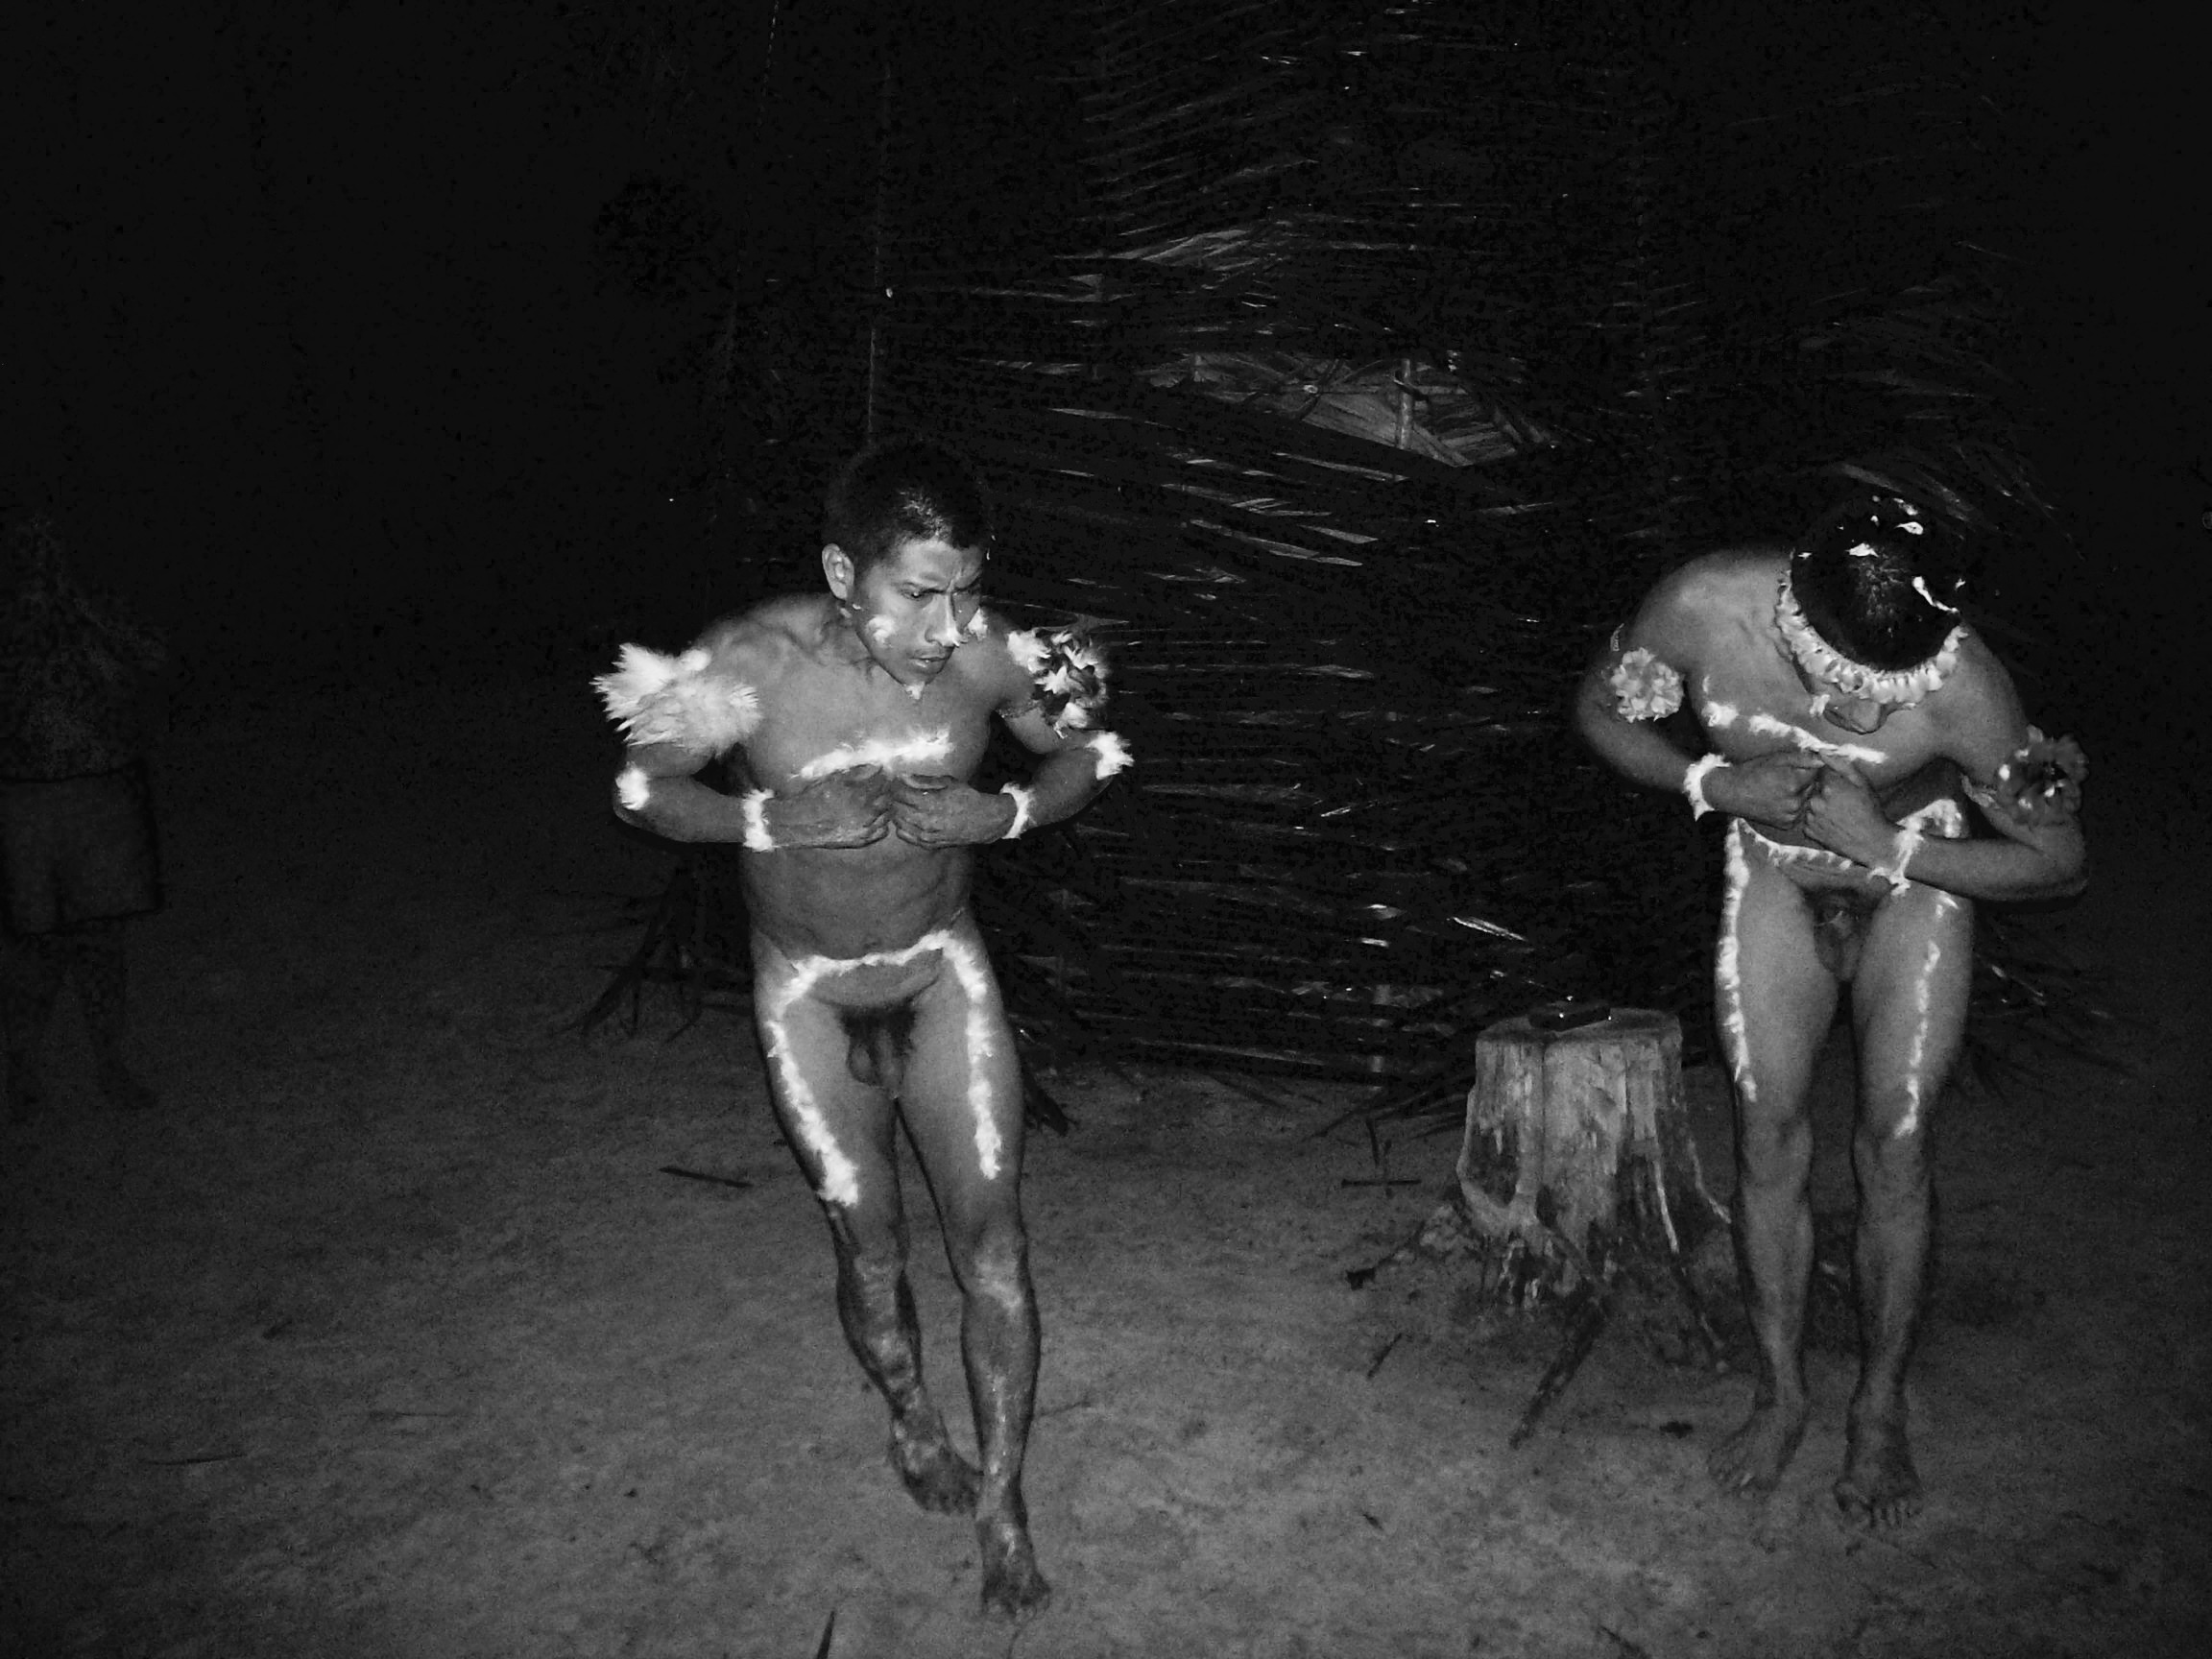
\includegraphics[width=\textwidth]{./imgs/100_1695}
%\caption{Os homens trazem os \textit{karawara} à noite. Ao fundo se vê a \textit{takaja} (aldeia Juriti, 2009).}
%\end{figure}

A construção da \textit{takaja} Guajá não obedece a nenhuma prescrição
ritual ou regra de conduta, diferente, por exemplo, da ``\textit{tokasa}''
dos Asurini Akuawá. Andrade observa que para os Asurini ``a colocação das
folhas é feita de tal forma que o construtor termina a tarefa dentro da
\textit{tokasa}. Ele só pode sair de dentro após cantar a \textit{música}
\textit{da} \textit{tokasa} {[}\ldots{}{]}. Caso a canção não seja logo executada
(pelo construtor ou outra pessoa que a saiba), o construtor pode morrer''
(Andrade, 1992, pp.\,99--100). Se o evento noturno é de pouco
cerimonialismo e marcado por grande informalidade, como veremos, a
construção da \textit{takaja}, então, se parece com uma atividade
ordinária, quase sem importância. Eu mesmo fui instado diversas vezes
para entrar e conhecer a \textit{takaja} por dentro (sempre durante o dia,
pois à noite tudo é diferente). Ainda que seja construída de uma forma
um tanto deslustrada (sem prédica, cerimônia, ou um mínimo cuidado
ritual), a construção da \textit{takaja} é algo que produz grande alegria
a todos, principalmente às crianças que inserem o abrigo ritual em suas
brincadeiras diurnas, entrando e saindo livremente de lá; ou ainda às
mulheres, que fazem questão de varrer o entorno, antes e depois de ela
ser erguida, e assim passam varrendo durante todo o verão. A
\textit{takaja} na aldeia, nos meses de seca, é algo que os Guajá apreciam
bastante, até guardam certo orgulho por tê-la ali. Porém é um orgulho
que não parece diretamente relacionado ao cerimonialismo ou qualquer
tipo de sermão, mas a algo de outra natureza --- que eu não saberia
precisar ---, como que relacionado à boa vida do verão e ao prazer que os
homens cultivam em ir ao \textit{iwa} e cantar com os \textit{karawara}. Na
aldeia juriti, a takaja fica exatamente no centro da aldeia, mas nem
sempre foi assim. Os Guajá se lembram que, quando viviam na mata,
construíam a tajaka sempre em um canto da aldeia, a caminho da floresta.
Assim ela é feita na aldeia \textit{Awá} (\textsc{ti} Caru) na última sessão
residencial, já a caminho de uma capoeira. A \textit{takaja} não funciona
como uma ``casa cerimonial'' em um pátio central, que congregaria homens
e deuses; ela é um elemento bem mais discreto e minimalista, assim como
é todo o investimento ritual dos humanos, \textit{awa}.

Descrever a \textit{takaja} dos Guajá é quase que descrever um não ritual.
Algo como expor apenas ``negatividades'' em uma interminável lista de
``elementos rituais'' que não encontramos lá. Na composição desse ritual
--- que também podemos chamar de ``cantoria'', \textit{janaha}, como fazem
os próprios Guajá ---, o ambiente da aldeia em nada se modifica durante as
noites em que ele ocorre: nada é levado ao pátio; nenhuma reza é
realizada; comidas não são preparadas cerimonialmente; e nem mesmo a
caça de animais específicos está prescrita, isto é, não há caças
rituais. Além disso, não há flautas, cigarros, mingaus, bebidas
fermentadas, danças com animais; nem distinção entre ``alimentos
cotidianos'' e ``alimentos rituais'',\footnote{Sobre ocorrências em 
outros povos, tais como os Parakanã, ver Fausto, 2001, p.\,422.} até porque não
existem alimentos no ritual. Observo que, se antes a ideia de \textit{awa
janaha}, ``cantoria humana'', expressava o momento ritual da
\textit{takaja}, mais recentemente, sobretudo, os Guajá da \textsc{ti} Caru --- onde
há um trabalho de parceria com o \textsc{cimi} --- têm também se referido a ela por
meio de ideias como ``ritual'' e ``cultura''; ou ao menos a estão,
assim, explicando para os interlocutores não indígenas, como a Frente de
Proteção da Funai. É interessante, pois a primeira tradução em português
que encontrei para a ideia de ``cantar na \textit{takaja}'', ainda na
aldeia Juriti, foi a de ``brincadeira'' ou simplesmente ``brincar''
(\textit{pirika}, na pronúncia Guajá). Todos os homens, inclusive os
velhos, vinham falar comigo sobre ``\textit{pirika}'', que eu no início
entendia como ``brigar'', nos dias que cantariam na \textit{takaja}. Essa
tradução fora-lhes fornecida pelas pessoas das Frentes de Atração e
funcionários do posto que se referiam ao ``\textit{karawara}'', tal a
forma que os brancos denominam a \textit{takaja} guajá, pelo mesmo termo
que outras festas maranhenses, como o bumba-meu-boi, todas elas --- no
Maranhão e em boa parte do Brasil --- chamadas popularmente de
``brincadeira'' --- ``brincar o boi'', como se fala no Maranhão. Mais
recentemente, ao menos nas aldeias Awá e Tiracambu (na \textsc{ti} Caru), a ideia
de ``brincadeira'' está cedendo lugar a ``ritual'' e ``cultura''.

À exceção da \textit{takaja}, a única preparação especial está no fato ---
desde alguns dias antes de sua montagem --- de que algumas pessoas se
mobilizam para capinar e limpar todo o mato acumulado durante o inverno
no centro da aldeia. Uma vez o pátio limpo, pode-se começar a montagem da
\textit{takaja}, que é erguida em pouco tempo: cerca de 40 minutos. No
início da noite, os homens começam a entoar seus cantos de maneira muito
potente. E, aos poucos, começam a se adornar. Suas esposas os ajudam a
se paramentar. Quando um homem é solteiro (ou sua esposa ainda é
criança), recebe o auxílio de sua irmã, cunhada, ou até mesmo de outro
homem. A ornamentação consiste em braceletes com penas de tucano,
chamados \textit{jamakwa}, e um cocar formado com as mesmas penas, chamado
\textit{jakỹ ita}. No corpo --- coxas, virilha, torço, braços, rosto e em
volta dos pulsos, como um bracelete --- e nos cabelos são afixadas
penugens brancas da harpia, gaviões ou urubu-rei. Estas são presas com
resina cheirosa de dois tipos de amescla (breu-branco), chamadas
\textit{jawarako} (\textit{Trattinnickia burseraefolia}) e \textit{uhuka} (que
não identifiquei). Tais resinas, além de fixar as penas, exalam um odor
muito agradável, mentolado, que é o próprio cheiro dos \textit{karawara}.
Os braceletes de penugem branca podem ser feitos de duas formas: as
penugens são coladas diretamente no pulso com a resina; ou são amarradas
na fibra de tucum, como uma pulseira atada ao punho. Uma vez
paramentados, podem ir para o céu.

A noite já se instalou, e a partir de agora quanto menos luz perto da
\textit{takaja}, melhor. Enquanto se adornam, os homens cantam, e uma vez
prontos se dirigem ao abrigo cantando e dançando com passos específicos:
as duas mãos entrelaçadas sobre o peito e, sem mudar a postura das mãos,
levantam e abaixam o corpo como os movimentos de uma ave a ciscar o
chão. Esta é uma das danças --- \textit{panỹ}, ``dançar'' --- executadas pelos
\textit{karawara} no céu e imitadas pelos humanos na Terra. A única
luminosidade em volta da \textit{takaja} vem de uma casa em que um fogo
queima bem baixinho para espantar o frio. A escuridão é uma das marcas
desse momento ritual. Os \textit{karawara} só descem à Terra na escuridão,
pois, mesmo vindo caçar durante o dia, não gostam da luminosidade
terrena. É importante lembrar que toda cantoria na \textit{takaja} é
noturna, e podiamos pensar que, assim como para os \textit{xapiri} do
mundo Yanomami, nossa noite é o dia para os \textit{karawara}.\footnote{Kopenawa e
Albert, 2013, p.\,55.} Os humanos, por isso também, nunca cantam ou dançam
cerimonialmente durante o dia; tampouco existem festas que durem dias
seguidos. Se a \textit{takaja} for feita durante noites seguidas (o que
varia muito), tudo é interrompido na madrugada. Nesse caso, no dia
seguinte todos voltam a suas atividades cotidianas, e à noite uma nova
sessão é iniciada.

A cantoria e a dança se iniciam enquanto, um de cada vez, os homens
adentram para cantar na \textit{takaja}. No início, o clima é de grande
informalidade. Enquanto algumas pessoas estão completamente envolvidas
na cantoria, outras vêm e vão ainda procurando uma refeição para fazer.
Pessoas que não estejam diretamente envolvidas conversam bem alto como
se nada de mais especial estivesse ocorrendo. As crianças correm em
volta da \textit{takaja}, fazendo algazarra, enquanto os adultos estão
compenetrados em cantar. No entanto, nenhum desses acontecimentos afeta
a dinâmica do evento. Lembro aqui que, no falar dos \textit{karawara},
cantar é \textit{myry} e não ``\textit{jã}'' como na língua guajá. E na
\textit{takaja}, ao menos nas canções, é observada a língua celeste, que
pode ser traduzida também como uma ``linguagem ritual''. Nesse caso, no
falar dos \textit{karawara}, fala-se \textit{imyry ta iwapepe jaha}, ``eu
vou cantar no céu''.\footnote{Sobre os \textit{karawara} falarem outro
  idioma, Calheiros também observa algo semelhante nos
  ``\textit{karuwara}'' Aikewara: ``{[}\ldots{}{]} eles (os \textit{karuwara}) não
  são ``aqueles que se foram'', eles não são seus mortos, seus
  ancestrais, eles são outros, são seus inimigos, falam, inclusive, uma
  outra língua, incompreensível aos ouvidos de um Aikewara médio, uma
  língua que somente os \textit{se'engara'e} (xamãs) dominam (Calheiros,
  2014, p.\,266).}

Uma vez dentro, o homem inicia uma sucessão de cantos que são entoados
com toda força, quase sempre se iniciando com o \textit{Makaro janaha},
``canto do (\textit{karawara}) \textit{Makaró}'', que, como já mencionei, é
quase que uma epítome de um grande caçador de porcos e do que sejam os
próprios humanos hoje em dia. Do lado de fora da \textit{takaja}, homens,
mulheres e, por vezes, nos momentos iniciais da noite, crianças, seguem
cantando. É possível perceber o som da voz masculina no interior da
\textit{takaja} se deslocando de um lado para outro, já que o homem que se
encontra dentro está dançando em movimentos circulares. De repente
ouve-se o barulho de um salto e um silêncio mortal no interior do
abrigo: o homem foi para o céu; ``\textit{oho iwa}'', alguém comenta.
Nessa hora, a esposa, irmã ou qualquer outra mulher ligada ao viajante
celeste inicia um canto frenético. É só a partir daí que podemos
enxergar a importância das mulheres durante a cantoria, pois sem elas
dificilmente os homens conseguiriam voltar para casa --- \textit{iwy},
``voltar''. Após subir ao céu, um homem pode permanecer lá por um tempo
relativamente longo que, até onde presenciei, pode variar de 15 minutos
até algumas horas, embora a média talvez seja de meia hora, enquanto o
momento ritual em si pode durar desde duas até seis horas, ou mais.

Wirahoa me explicava que se as esposas não cantassem aqui na Terra, o
marido que estivesse no céu não conseguiria encontrar o caminho de volta
para casa, pois, devido à vastidão do lugar e aos diversos céus que ele
visita em sua viagem, seria muito fácil se perder por lá. O canto das
esposas é o único elo que permite a conexão do céu e da Terra. Enquanto
seus maridos estão na viagem celeste, as mulheres cantam daqui e são
ouvidas por seu duplo celeste, \textit{nima}. Os solidários duplos
celestes das esposas falam ao homem: ``volte para a Terra, \textit{ajwy}
\textit{wype}, volte para ouvir sua esposa cantar, ela está te chamando!''
Por isso, todo canto feminino durante as noites de \textit{takaja} é uma
espécie de chamamento para que o homem volte para casa. Para que não
morra no céu.

Em uma madrugada, já muito tarde, Muturuhũa havia restado sozinho na
\textit{takaja}. Todos já haviam cantado bastante e --- depois de muitas
idas e vindas ao céu --- foram dormir. Muturuhũa foi o último a entrar na
\textit{takaja} e, aparentemente, não havia ninguém para cantar para ele,
pois sua esposa Amỹ Pirawãja estava deitada na rede. Assim que o homem
entrou na \textit{takaja}, a mulher sequer abriu os olhos ou mudou de
posição, mas mesmo deitada em sua rede iniciou um canto baixo e
constante, o suficiente para que seu marido fizesse uma boa viagem. É
claro que outras e outros podem cantar (irmãs ou irmãos, cunhadas ou
filhas); nada o impede. Porém, é muito comum que a esposa cante para o
marido. Ela, portanto, é fundamental em todo o processo de ``ida para o
céu'', \textit{oho} \textit{iwape}. Sem ela não há viagens celestes nem o
momento ritual na \textit{takaja}. A conjugalidade pontua todo esse
processo, pois são as esposas celestes que cantam, ``lá em cima'', 
\textit{wate}, o canto das esposas terrenas. São elas que ouvem as
mulheres da Terra, que para elas são \textit{hapihiara}, seus ``duplos'', e
informam o caminho de volta aos Guajá que estão no céu e, sobretudo, que
é hora de voltar. Minha hipótese é que não podem existir viagens ao céu
(e portanto xamanismo) sem que os homens estabeleçam algum tipo de
relação conjugal com mulheres \textit{karawara}. Essas esposas celestes,
muitas vezes, descem à \textit{takaja} a fim de procurar por seus maridos
terrenos, como aconteceu certa vez em que Wirahoa estava ausente da
aldeia (talvez estivesse no caminho de volta de uma caçada). Sua esposa
Ajruhua foi chamada por outras pessoas para perto da \textit{takaja}, pois
a esposa celeste, \textit{iwa} \textit{nimirikaa} --- assim me foi dito ``a
esposa'' e não ``uma esposa'' --- estava querendo ouvir-lhe cantar. Mas, como
todos os \textit{karawara}, ela voltou rapidamente para o céu. Quando
conversei depois com Ajruhua sobre a situação, ela respondeu muito
tranquilamente: ``é a mulher do céu, ela veio procurar o marido dela, mas
ele tá caçando!'' O ``marido'' em questão era seu próprio marido.

Enquanto seus pares cantam em volta da \textit{takaja}, um homem, ao
adentrá-la, permanece no interior ainda por alguns minutos, cantando e
dançando até que consegue subir. Assim como acontece nos sonhos, \textit{imuhy}, 
o \textit{ipirera}, ``couro'', o corpo da pessoa, permanece
no interior da \textit{takaja}, despossuído de seu \textit{hajtekera}, ``princípio vital''. 
É, portanto, o \textit{hajtekera} que se desprende do
\textit{ipirera}, do corpo, e viaja até o céu, \textit{iwa}. Chegando ao
\textit{iwa}, depois de muito subir, o homem encontra o primeiro patamar
onde só há daquela água quente, '\textit{ya} \textit{haku}, e que, à época
das chuvas, inunda a Terra na forma de grandes temporais. Durante o
verão, quando ocorrem os cantos da \textit{takaja}, o nível de água nesse
primeiro patamar é muito baixo, a lama toma o lugar das águas e o grande
lago de águas borbulhantes e vermelhas lá existente está praticamente
vazio --- esse patamar, também chamado \textit{iwa}, não tem nenhum nome em
especial. A única condição para se fazer a \textit{takaja} é que o período
das chuvas já tenha terminado.

Para chegar à aldeia dos mortos e dos \textit{karawara} é necessário
atravessar este céu intermediário. Uma vez neste primeiro patamar, o
viajante celeste não deve permanecer muito tempo, pois além das águas
borbulhantes --- que já mataram muitas crianças \textit{karawara} acidentalmente caídas 
nesse lago --- lá vivem jacarés, \textit{jakarea}, grandes e
famintos, que, segundo algumas versões, comeriam os humanos que lá
chegam. Por isso, deve-se subir novamente e, agora sim, alcançar a
morada dos \textit{karawara}, também chamada \textit{karawa} \textit{ripa},
``aldeia dos \textit{karawara}'', local onde estão os \textit{harapihiara}
(parentes próximos, cognatos) e \textit{harapihianã} (parentes distantes,
não cognatos), pois os Guajá defendem fervorosamente uma semelhança
direta entre eles e os \textit{karawara}. A partir daí, os cosmonautas
podem acessar outros muitos patamares celestes, que são incontáveis.
Além disso, como escrevi no primeiro capítulo, o ``céu intermediário'' das águas
quentes não é justaposto aos outros \textit{iwa,} mas se encontra
deslocadamente abaixo. A terra dos \textit{karawara} estaria mais para
cima e para frente, bem distante da \textit{wy}, a Terra. O céu que podemos
observar, estando na Terra, é somente este céu intermediário, a primeira
parada dos homens quando estão em trânsito.

Subir é perigoso, sempre. É uma atividade ultra especializada. Os
\textit{karawara} convidam insistentemente os homens para que subam ainda
mais, a outros céus, para que comam banquetes magníficos em outras
aldeias; para que adquiram outras esposas celestes; conheçam outros
seres; ouçam outros cantos e vejam outras danças. Os humanos, no
entanto, sabem que isso implicaria sua morte, já que, devido à
distância, não ouviriam mais suas esposas cantando e se perderiam para
sempre. Não se deve andar, \textit{wata}, muito no \textit{iwa}. O canto das
mulheres terrenas é ouvido como um canto de procura, e os homens falam
para os \textit{karawara}: ``estão ouvindo a minha esposa cantar na Terra?,
ouçam, ela está me procurando, por isso está cantando, tenho que
voltar''. Os \textit{parentes} celestes ainda perguntam sobre as mulheres
terrenas, pois nutrem grande interesse por elas. Os humanos devem
explicar que elas ficaram na Terra, pois não podem subir, mas os
\textit{karawara} insistem para que os humanos as levem até lá. Uma vez,
ao serem indagados por mim sobre a possibilidade de as mulheres irem ao
\textit{iwa}, foram taxativos dizendo que elas não podem ir, pois não
saberiam como chegar, além de serem cobiçadas pelos \textit{karawara}
celestes. Em outras palavras: elas morreriam. Estamos vendo então que,
por baixo de um verniz de bem-aventurança e satisfação, há também morte
e disputa por mulheres, envolvidas na relação entre \textit{awa}, ``humanos'',
e \textit{karawara}, cabendo aos humanos administrar esta tensa e delicada
relação. Quando as pessoas mencionam essa comunicação melódica entre
mulheres na terra e homens no espaço celeste, afirmam que o canto das
mulheres não são apenas um canto de referência para os homens ouvirem
desde o céu, mas se trata de um diálogo como certa vez Wama'axia (uma mulher
da aldeia Tiracambu) me revelou. Ouvindo uma gravação de aúdio de quando
seu pai Akamatỹa estava no céu e sua esposa, Pinawãxika, cantava na
terra, ela explicou que naquele canto a mulher falava ao homem ``volte
para casa'' ``você já comeu?'', e em paralelo o marido cantava ``eu já
comi guariba'' e ``agora eu cheguei aqui no chão'' (voltei do céu). Essa
comunicação entre esposas que cantam da terra e homens que as escutam do
céu é, além de poética, metafisicamente complexa, pois os homens podem,
só pelo fato de responderem à esposa, voltar à terra imediatamente.
Imagino que, se tirarmos por esse caso específico, a própria palavra de
uma mulher pode produzir a volta do marido. As evidências são sempre
baseadas em fragmentos como esse acima, pois assim também o é o estilo
vocal Guajá, cheio de cortes, repetições e paralelismos (com duas pessoas
cantando em paralelo em ``diálogo'' ou não).

A visita dos humanos ao \textit{iwa}, durante a \textit{takaja}, é, lá nos
patamares superiores, marcada por canto, \textit{janaha}, dança, \textit{panyha}, 
e comensalidade, \textit{i'uha}. É disso que tratam os
encontros celestes, uma vez que caçar (e comer) e cantar é o que marca
boa parte da vida humana. Os diversos \textit{karawara} entoam seus cantos
característicos e o fazem sempre de uma forma mais bela que os
visitantes humanos; e ainda pedem para que os humanos cantem. Os
\textit{karawara} ainda dançam com suas flechas energizadas nas costas,
coreografias repletas de brilho; são as mesmas flechas que utilizam para
caçar na Terra e que matam suas presas sem lhes causar ferimento. Os
raios do céu, principalmente aqueles que aparecem à noite, são o
resultado das flechas com energia, \textit{tata}, desses \textit{karawara},
e quando alguém olhar para o céu e notar os raios, certamente exclamará:
``\textit{karawara} \textit{panỹ!''}, os ``\textit{karawara} estão dançando!'' Por
isso, na Terra, outra forma de os homens dançarem fora da \textit{takaja}
é colocarem cera de maçaranduba ou jatobá na ponta de uma taquara, ou
outra madeira fina, acender e dançar com ela apoiada sobre os ombros,
tal como os \textit{karawara} com suas flechas, o que causa um efeito
visual fantástico. Há ainda dois \textit{karawara} chamados \textit{Japu}
\textit{Jara} (pássaro japu) e \textit{Japini'i Jara}, ``xexéu'', que, por serem
construtores de tapiris no céu, lá dançam com palhas sobre as costas.
Por isso os homens, ao cantar seus temas na \textit{takaja}, dançam
segurando palhas secas nas costas, como esses \textit{karawara}.

Quanto à comensalidade, ela parece ser uma espécie de ``oferenda às
avessas'', diferente de outros povos Tupi que preparam rituais com
banquetes específicos para suas entidades sobrenaturais que aqui descem
para se alimentar (como já expus anteriormente). Entre os Guajá, são os
\textit{karawara} que lhes oferecem comida. Como já sugeri, há grande
fartura no \textit{iwa}, já que os caçadores magníficos que lá habitam
conseguem carnes com tanta facilidade que nem sequer as estocam. Além
disso, a farinha é branca e quase doce, \textit{hee'ẽ}, de tão gostosa, os
frutos são maiores e as quantidades de mel, descomunais. Desta forma os
\textit{karawara} disponibilizam toda essa fartura para os humanos que lá
conseguem chegar, quase que um oposto do que vemos em outras formas de
xamanismo, em que são os deuses que descem para comer. Os homens que
alcançam o céu são unânimes ao lembrar que os \textit{karawara} tentam
prendê-los lá pela fartura e abundância das refeições.

Assim, uma vez no \textit{iwa}, um homem encontra seus parentes, canta e
come com eles, escutando seus conselhos, desde a escolha de um nome,
notícias sobre caçadas, sobre a cura de enfermos (quando existem), e até
mesmo bens são disponibilizadas pelos \textit{karawara}. Wirahoa confirmou
já ter trazido alguns cartuchos (de espingarda calibre 20) que ganhou de
presente dos \textit{karaia} celestes. Pessoalmente, tive o prazer de
presenciar a preparação dos caçadores para uma caçada de porcos, cujo
rastro da vara aparecera no dia seguinte a uma noite de cantoria na
\textit{takaja}. Wiraho me disse com tranquilidade que havia pedido para
seus \textit{parentes} mandarem os animais para que fossem caçados. Nunca
encontram \textit{Maira} no \textit{iwa} durante a época em que sobem, pois
o verão, \textit{kwarahy mehẽ}, é a época em que \textit{Maira} (além de
alguns \textit{karawara} que não saberia apontar) se ausenta para longe e
vai para a ``casa de seus sogros''. Durante as noites de \textit{takaja},
os Guajá só se encontram com os parentes mortos (tornados
\textit{karawara}, como veremos logo adiante), além dos \textit{tenetehara},
dos \textit{karaia} celestes e dos diversos \textit{jaras} que já elenquei.

\section{\textit{aru karawara}, «trazer os \textit{karawara}»}

Uma das coisas mais impressionantes no momento ritual da \textit{takaja},
tanto quanto a subida dos homens ao céu, é a descida dos \textit{karawara}
para ali cantar e dançar. Uma vez que um homem vai para o céu, o
silêncio reina no interior da \textit{takaja}; só é ouvido o som da
cantoria externa, sobretudo das mulheres. Esse estado permanece por
longos minutos (10, 15 ou mais). Todavia, passado algum tempo as folhas
da \textit{takaja} tremulam de cima abaixo e ouve-se o barulho de um pulo:
dois pés pisaram o chão simultaneamente, o que indica que algum
visitante celeste veio à Terra, \textit{wya}, cantar. Quando sobem, seu
\textit{ipirera} (corpo) fica no interior da \textit{takaja}, vazio,
utilizado como uma pele pelos \textit{karawara} (sejam, onça, gavião,
pássaros, marimbondos, \textit{karaia}, \textit{tenetehara} e a infinidade
de seres que vive no \textit{iwa} e desce para cantar). Para quem sobe ao
céu é dito que ``traz os \textit{karawara}'', \textit{ru} \textit{karawara}; uma
vez no \textit{iwa}, ele diz aos seres de lá: ``Desçam, vão ver seus
parentes na Terra!'' Alguns são bem-vindos, outros (como as onças
celestes) devem ser espantados. Para isso, uma criança, se alguma ainda
estiver acordada, uma mulher ou um homem bate com vigor nas paredes de
folha da \textit{takaja}. Um pedaço de pau, \textit{wira}, é utilizado para
bater, visando a enviar o visitante indesejado de volta para o céu. A
\textit{takaja} é um local perigoso, pois é aberta a diversos tipos de
seres, inclusive a alguns que intentam levar esposas da Terra, ou mesmo
sair da \textit{takaja}. Por isso, os homens que os trazem devem se
entender bem com eles e, em alguns casos, as pessoas os devem espantar
de volta, batendo nas paredes. Durante a cantoria, não é permitida a
entrada de nenhuma mulher ou criança no abrigo.

A \textit{takaja} Guajá, tal como ocorre com outros povos, como os
Parakanã (Fausto, 2001, p.\,281) e Asurini do Xingu (Müller, 1990,
pp.\,151--154), seria algo como um ``aprisionador ou receptáculo de
espíritos'' (Fausto, 2001, p.\,281), tal uma transformação do maracá, como
pontua o autor:

\begin{quote}
A ideia de que os espíritos se manifestavam através dos maracás porque
estavam dentro dele é expressa por autores que consolidaram o material
quinhentista: `o maracá, instrumento sagrado dos tupinambás, possuía uma
função definida nos rituais, parecendo fora de dúvida que estava nele o
espírito envocado (Fernandes, 1970, pp.\,75--76); `o maracá servia de
receptáculo ao espírito' (Metraux, 1979, p.\,60). O maracá seria, pois, uma
tokaja, que atrai e contém os espíritos, os quais só os pajés eram
capazes de ouvir.\footnote{Fausto, 2001, p.\,281.}
\end{quote}

A \textit{takaja} aqui, tal a analogia de Fausto a partir do material
quinhentista, pode ser pensada como esse grande objeto atrator e
aprisionador e parece operar como um grande instrumento musical, uma
grande caixa de ressonância para os \textit{karawara} que descem à Terra
para cantar.

Cada \textit{karawara} detém especificidades em seus cantos, de modo que
todas as pessoas que estão do lado de fora da \textit{takaja} sabem
exatamente qual ser está em seu interior. E todos descem à
\textit{takaja}: onça, \textit{jawara}, papa-mel, \textit{haira}, jiboia, 
\textit{majhua}, jacaré, \textit{jakarea}, gavião, \textit{wirahoa},
pererecas, poraquê, \textit{marakya}, dentre outros. Além desses, os
\textit{karaia} e \textit{kamara} celestes também descem. Os \textit{karawara}
que descem do céu, além de cantar, emitem os sons característicos de
seus duplos terrestres, sugerindo que, sim, os \textit{karawara} são
versões humanas e celestes --- isto é, duplos --- de animais terrenos. Os
Guajá dizem que quem emite os rugidos e cantos de animais são os filhos
dos \textit{karawara} que os acompanham à \textit{takaja}, pois esses, por
serem crianças, ainda não sabem cantar. Desta forma, é possível ouvir a
onça e seu rosnado; o som gutural de porcos; o canto do gavião; e até
mesmo um improvável morcego, \textit{arira}, que aqui veio cantar. Alguns
seres animais, como os \textit{Jakara} \textit{Jara}, que vivem no patamar
alagado, e \textit{Wri} \textit{Jara}, um capelão agressivo de cor
vermelha, também vêm para a \textit{takaja}.

À medida que os homens saem da \textit{takaja} para cantar do lado de
fora, quem está ali são os próprios \textit{karawara}, que param em frente
as mulheres e crianças, cantam-lhes, sopram-lhes e por meio das canções
contam suas epopeias, falam sobre a saudade de uma Terra e um tempo
distante ou cantam as maravilhas que há no céu. Nas noites de
\textit{takaja}, as aldeias ficam repletas de \textit{karawara}. Esses
\textit{karawara} se relacionam diretamente com aquele homem específico,
como parceiros ou mesmo ``espíritos auxiliares''. Cada homem se
relaciona com um conjunto de espíritos específicos no céu, e são eles,
da confiança dos humanos, que descem à Terra. Após algum tempo no
\textit{iwa}, é o momento de o homem retornar. A descida, como me foi
relatada por Hajmakoma'ã, é suave e pode ser comparada à queda de uma
``folha''. Esta seria mais uma razão para os meninos jovens não irem ao
\textit{iwa}: eles não saberiam como descer, poderiam cair na descida e
morrer. É muito comum, nas primeiras tentativas de ida para o céu,
jovens de 15 anos tentarem subir e, mesmo paramentados, se frustarem em
tentativas de alcançar o céu. São necessárias muitas sessões iniciais
até que os jovens aprendam. Houve noites em que os homens tiveram que
ser breves, com uma duração ritual muito curta (cerca de duas horas),
pois o \textit{iwa} naqueles dias estava insuportavelmente quente, e os
humanos não aguentaram permanecer por lá. Em todo caso, é esse \textit{iwa
rakuha}, ``calor do céu'', que os \textit{karawara} trazem na descida à
Terra, sopram nas esposas e crianças do seu parceiro e que tem funções
terapêuticas.

O processo de cura consiste basicamente em trazer o ``calor do céu'', 
\textit{iwa} \textit{rakuha}, esse ar terapêutico que é soprado pelo
homem-xamã em diversas partes do corpo da pessoa. Esse calor, tanto atua
de forma preventiva, fortalecendo o corpo, como pode curar um enfermo,
se administrado em doses mais intensas. O que os \textit{karawara} fazem
na Terra é, primeiro, ``cantar'', \textit{jã}, e, depois, ``soprar'', \textit{pyy};
hoje em dia, muitas pessoas da \textsc{ti} Caru têm chamado isso de ``rezar'', em
português. A ideia do sopro é que as pessoas fiquem bem, sem doença:
\textit{a'e kĩja}: ``ficar assim todo tempo'', sem doença. Essa é uma das
funções do sopro, ``\textit{iku katy}'', ``ficar bem''. Os \textit{karawara}
entram no corpo do seu parceiro, ``irmão'', \textit{hapija perera},
``pele do irmão'', como que se vestindo com sua pele, \textit{ipirera},
para atuar na Terra. Outra forma de mencionar essas curas é \textit{ru
iwa} \textit{janaha}, ``trazer a música do céu''. Os \textit{karawara} e a
cura estão diretamente relacionados. É pelo canto que os homens se
comunicam com os \textit{karawara} que lhes auxiliam nas curas. O canto é
quase um bem material, algo externo produzido pelos \textit{karawara} e
utilizado pelos humanos.

Quando os \textit{karawara} descem do céu vestindo a pele dos humanos e
saem da \textit{takaja} em direção a suas esposas e filhos para soprá-los, 
\textit{pyy}, sempre haverá uma mistura entre \textit{karawara} e humano ---
é como se o homem o trouxesse junto com ele. E só quem vê os
\textit{karawara} são os homens que cantam e curam. Em outra
interpretação, os \textit{karawara} ficariam dentro da \textit{takaja}, e
quem sai seria o próprio homem para soprar. Segundo me informou Wirahoa,
os \textit{karawara} ``falam'' com os Guajá de dentro da \textit{takaja}.
Ideias como \textit{xá} \textit{iwa}, ``olhar o céu'', \textit{takaja janaha},
``o cantar da \textit{takaja}'', \textit{ru karawara}, ``trazer
\textit{karawara}'', e \textit{ru hakuha}, ``trazer o calor'', são todas
sinônimos para ``curar''. Enquanto os \textit{karawara} estão em Terra eles
sopram os vivos e tiram as doenças. Trata-se de um ``xamanismo padrão'',
acessível a todos os homens (quase como uma imposição de gênero), e está
longe de ser um conhecimento especializado. Se perguntarmos a qualquer
um, na aldeia Juriti, quem lá saberia ``tirar'' ou ``soprar'' doenças
--- \textit{hahy}, ``dores'' ---, todos os homens adultos serão apontados, pois
todos conseguem ir para o céu e trazer o ``calor'', o que não quer dizer
que todos tenham o mesmo nível de excelência. Por isso, Xiparamyxa'a, um
homem mais velho, é considerado o melhor curador da aldeia. Muitos
homens recorrem a ele quando eles mesmos não conseguem curar seus
parentes próximos. Lembro ainda que não encontrei um termo na língua
Guajá para o especialista em cura.

As doenças, como já vimos, têm causas variadas, e a terapêutica Guajá
mistura os cantos e os remédios tradicionais. Houve uma ocasião,
enquanto trabalhávamos na roça, em que encontramos um pequeno veado
foboca, \textit{arapaha'ia}, que logo fugiu. Na mesma tarde, o jovem
Juxa'a, que estava conosco na roça, caiu doente com muita febre e
calafrios. Sabemos que os veados são animais de criação dos \textit{ajỹ},
por isso lançou-lhe \textit{ha'aera}, ``raiva''. Naquela mesma noite, seu
padrasto teve que tirar-lhe a doença, \textit{hahy}. Tratava-se de um mês
de inverno, e nas chuvas os homens não sobem ao céu pela \textit{takaja},
trazem os \textit{karawara} para dentro de seus corpos com o canto, o
único agente concreto do xamanismo guajá.

Os Guajá não utilizam tabaco nem as bebidas fortificantes que seriam
consumidas pelo curador. O máximo que utilizam são os remédios da
floresta como auxílio da cura, porém o básico é o canto, \textit{jã}, e o
sopro, \textit{pyy}: o canto, para trazer o \textit{karawara}, e o sopro,
para tirar a doença. Além da \textit{takaja}, há pelo menos uma forma de
trazer os \textit{karawara} à Terra. São esses cantos noturnos, em casa,
na rede, quando o homem abandona seu corpo e traz o \textit{karawara} para
curar quem quer que seja. Quando um homem canta, o \textit{karawara} se
instala em seu peito que lhe comunica os procedimentos. É isso que
orienta os homens nas curas, tal como espíritos auxiliares. E o homem
canta ainda mais alto. Essas curas são chamadas simplesmente de
\textit{karawara} ou \textit{ru} \textit{karawara}, ``trazer \textit{karawara}'',
tal qual a acepção comum de ``feitiço'' que vimos em outras paisagens. Os
\textit{karawara} Guajá se conectam parcialmente com essa ideia de feitiço
e contra-feitiço, mas que não podem ser traduzidos literalmente assim,
pois, antes, são seres que dominam a cura, a qual também é chamada
``\textit{karawara}''. O agente terapêutico --- chamemos assim --- soprado pelos
homens, o calor do \textit{iwa}, serve para tirar o agente patogênico,
\textit{ha'aera}, do corpo das pessoas. Por isso, para os animais, o
\textit{ha'aera} é visto como \textit{karawara}. O ``\textit{ha'aera} é o
\textit{karawara} do capelão'', repetindo o que alguém me disse certa vez.

A cura feita sob orientação dos \textit{karawara} consiste em que o
homem-xamã molhe com saliva seus dedos indicadores e imprima pequenos
pontos úmidos nos braços, troncos, pernas, ou outra parte que esteja
dolorida ou doente. Após essas marcas serem feitas, deve-se soprar
bastante, além de cantar com intensidade. O sopro, tanto na
\textit{takaja} quanto durante a época das chuvas, nessas seções privadas,
é feito nos braços e na cabeça. Cada braço é soprado, ao fim de cada
sopro passa-se a mão, e o processo termina com um sopro forte na cabeça;
repete-se isso diversas vezes, interrompendo-se apenas para cantar. Esse
é o procedimento básico para tirar o \textit{ha'aera} de alguém que foi
atacado por esses princípios mortais. A saliva é dita esfriar o corpo, 
\textit{ipirera}, da pessoa que estiver com febre. Se o fígado (órgão
destacado como de grande importância vital) estiver ruim, por exemplo,
imprimem pontos de saliva na barriga e costas; o mesmo ocorre com o
coração, dores nas juntas, musculares, cabeça, ou qualquer outra parte
magoada. Eu não saberia explicar a função da saliva nesse processo, mas
ela parece oscilar entre um antitérmico, condutor do sopro e uma espécie
de abridor de poros por onde o sopro entraria. De forma análoga,
descrevendo uma sessão xamânica, Fausto destaca que na cura Parakanã,
aquele que controla e sonha com os xerimbabos oníricos, além da fumaça
do cigarro e do sopro, esfrega sua saliva no corpo do enfermo a fim de
lhe imprimir a devida cura (Fausto, 2001, p.\,373).

\begin{center}\adforn{68}\end{center}

Para finalizar esse tópico, o rodízio de homens que entram na
\textit{takaja} segue uma ``ordem'' estabelecida de acordo com a situação.
Se participam cinco homens, o primeiro a entrar será o primeiro a
reentrar na \textit{takaja}, depois que todos seus companheiros já o
tiverem feito. À medida que um homem sai da \textit{takaja}, outro entra
imediatamente, ela não permanece vazia nem por um minuto. Depois de
outro período, entra um terceiro, e assim sucessivamente. A ordem
inicial parece aleatória, porém, quando o último homem a entrar sai da
\textit{takaja}, o que iniciou o processo retorna a ela, e a mesma ordem é
obedecida. Na aldeia Awá (\textsc{ti} Caru) acontecia também de entrarem dois
homens ao mesmo tempo. Depois de duas ou três entradas na \textit{takaja}
(e algumas boas horas de cantoria), já é alta madrugada, o relógio marca
três horas da manhã, e à medida que os homens saem do abrigo ritual,
voltam para suas casas levando o calor do céu para soprar em seus filhos
e esposas. A ``brincadeira'' (para evocar uma tradução indígena) acaba
gradativamente. O silêncio vai nublando a aldeia. Em seu pátio central,
só restará uma mulher, solitária, cantando para que seu marido retorne
em segurança do \textit{iwa}, para, então, poderem dormir em paz naquela
noite.

\section{ritornelo}

``Depois que morre, vira \textit{karawara}!'', é o que muitos diziam quando
conversávamos sobre a morte. Ao falarem sobre a morte, empregam como
sinônimo o verbo ``subir'', em português. Além disso, na língua
Guajá morrer, \textit{manũ}, é referido como \textit{oho iwape}, ``ir para o
céu'', a mesma ideia utilizada para descrever o momento ritual da
\textit{takaja}; ou ainda \textit{ikwẽ iwape}, ``permanecer no céu''. Além
dessas, outra forma pela qual se referem à morte, \textit{manũ}, é
\textit{karawara} \textit{pyhy}, literalmente, ``os \textit{karawara} pegaram''.
Os Guajá não gostam de conversar sobre a morte e sobre os detalhes da
nova vida que um dia todos experimentarão no \textit{iwa}. ``Eu não sei
não, Uirá!'', era o que me respondiam quando eu perguntava mais sobre os
\textit{karawara} (a quantidade de animais que esses seres caçavam; como
carregavam os animais para o céu; como tiravam embira para amarrá-los;
como ajudavam nas curas etc.); ou mesmo quando se tratava de discorrer
sobre a morte em geral.

Existe um \textit{karawara} chamado \textit{Kirimixixa'a} que é o
responsável por ressuscitar o morto quando este chega no \textit{iwa}
(cujo duplo terreno é um tipo de marimbondo que vive na beira de rios e
igarapés e, segundo os Guajá, ``gosta de cavucar a terra''). Lembremos
que, após a morte, é o \textit{hajtekera}, o ``princípio vital'', que vai
para o \textit{iwa}. Portanto, é essa parte da pessoa que renasce no
\textit{iwa}, em forma de \textit{karawara}. Quando um morto chega ao
\textit{iwa}, \textit{Kirimixixa'a}, que é uma espécie de xamã celeste,
habitante de um patamar distante, é avisado por seu filho. Então, ele
desce até os patamares inferiores, que é onde chegam os mortos. As
feridas do morto são limpas com aquela mesma água vermelha e quente, 
'\textit{y rakua}, que só existe no \textit{iwa} e que os humanos não podem
pisar, nem os \textit{karawara} podem beber. Trata-se de uma água curativa
capaz de cicatrizar qualquer ferida e esquentar um \textit{hajtekera} que
jaz frio.

Deitado, desfalecido, em uma rede de fibras brancas, a pessoa é soprada, 
\textit{pyy}, por \textit{Kirimixixa'a}. Este é o sopro que auxilia na cura
das feridas e no alívio das dores. Além do sopro e da água
ressuscitadora, esse \textit{karawara} lança-lhe \textit{tata}
\textit{hatỹma'a}, ``fogo-energia saudável-forte'', a mesma energia
brilhante produzida pelas flechas mágicas dos \textit{karawara} quando
dançam, que são vistas como raios, ou caçam, que matam a caça sem a
ferir, e ainda compõem os cartuchos dos \textit{karawara} que caçam com
espingarda. Uma energia brilhante, como o \textit{flash} de minha máquina
fotográfica, constituinte de vários fenômenos do \textit{iwa}. Após esses
cuidados, \textit{Kirimixixa'a} adorna o recém-chegado tal como um
\textit{karawara}: se for um homem, com as respectivas penas e cocares;
caso seja uma mulher, com a saia de penas de tucano confeccionada por
sua esposa. Após adornado e curado, \textit{Kirimixixa'a} envolve o morto
na rede, \textit{ikaha}, em que está deitado --- tal como um casulo. Após
abrir a rede, o morto está ressuscitado como um \textit{karawara}.

Quando acordar no \textit{iwa}, o recém-chegado tem vontade de voltar à
Terra para rever sua esposa e os filhos. Mas os \textit{karawara} não
deixam que isso ocorra. Em pouco tempo, o morto passa a guardar poucas
lembranças, \textit{imarakwaha}, de sua vida terrena, até esquecer
completamente que um dia foi humano. A vida como \textit{karawara}
facilmente suplanta a vida como \textit{awa}. Após a morte de
Pinawataxa'a, em 2009, seu irmão, Wirahoa, me disse que o encontrou no
\textit{iwa} na ocasião de uma \textit{takaja}, passados poucos meses após
sua morte. Nessa ocasião, Pinawataxa'a, o recém-morto, se recordava
muito pouco de seu irmão que ia lhe visitar no céu. Wirahoa me explicou
que, por haver muita comida, mulheres e belezas no \textit{iwa}, é fácil
esquecerem a vida na Terra, \textit{wya}. É por esse mesmo motivo que os
humanos devem esquecer completamente o morto, tal como um processo de
duplo esquecimento: em que os mortos --- estando lá --- esquecem os vivos; e
os vivos --- estando aqui --- esquecem os mortos. Quanto à ``vida eterna''
--- \textit{ikwẽ iwape}, ``permanecer no céu'' ---, ouvi tanto que os
\textit{karawara} nunca envelhecem quanto que têm o dom do
rejuvenescimento eterno e são tornados jovens a cada vez que envelhecem,
pelo mesmo processo energético de \textit{Kirimixixa'a}.

Se morrer é subir, como me relataram inúmeras vezes, o momento ritual na
\textit{takaja}, também dito subir, ou \textit{oho iwape}, ``ir para o céu'',
é uma pequena experiência de morte. Os homens que vão para o \textit{iwa}
durante essa cerimônia chegam vestidos como mortos\textit{karawara}, com
vestes idênticas às que utilizarão um dia, após lá renascerem como
\textit{karawara}. Os homens, tal como xamãs (embora essa função entre os
vivos não seja explícita), experimentam em vida --- com suas vestes,
canções e viagens ao céu --- as sensações que são vivenciadas plenamente
após a morte. Uma vida cheia de dança, canto e abundância.

Os \textit{karawara} se realizam enquanto ação pois existem como
entidades, e vice-versa. Pensá-los, porém, em termos identitários e
afirmarmos algo do tipo ``Os \textit{karawara} são desta ou daquela forma!''
não é o que sugiro aqui. Como vimos, eles são seres do tipo entidades
celestes, destino dos vivos, ao mesmo tempo que agem como agentes
noogênicos, do tipo substâncias extra naturais que realizam curas e
trazem saúde. Assim, os \textit{karawara} também parecem recolocar em
outros termos a relação \textit{riku} que --- se pelo entendimento da
conjugalidade e da propriedade (como no caso das flechas) é traduzida
por ``criar'' --- a relação dos \textit{karawara} com seus \textit{nima},
``versões'', ``duplos'', terrestres não sugere ``domínio'', nem ``controle'' ou
mesmo ``criação''; mas, sim, ``estar associado a''. A relação \textit{riku},
por isso, pode ser pensada como aquela que relaciona e associa seres,
não somente logicamente, mas consubstancialmente, e que, ora é uma
relação de ``criação'', ora de ``associação'', isto é, de ``estar com''. O
\textit{riku} é um processo de cognação entre diferentes seres do mundo:
maridos e esposas; pais e filhos; mulheres e animais de criação;
caçadores e suas flechas; humanos e duplos celestes; \textit{karawara} e
duplos terrenos; \textit{ajỹ} e animais; nomes e pessoas; animais
\textit{jara} e seus \textit{nima}, como a relação entre um veado e uma
paca; e tantas outras relações que vimos aqui. E essa ``teoria da
relacionalidade generalizada'' (para recolocarmos os termos de Viveiros
de Castro), cujos polos são denominados \textit{jara} e \textit{nima}, nem
sempre implicará controle ou domínio, como sugere o exemplo dos
\textit{karawara}.

A caça, como um ponto importante na vida dos Guajá, articula muitas
relações, como vimos, porém o objetivo deste livro, mais do que tirar
qualquer conclusão generalista, é explicitar e pôr
em relação diferentes aspectos da vida dos Guajá. Um mundo onde haja
caça abundante é fundamental, tanto para os Guajá, quanto para os
\textit{karawara}, caçadores que vêm caçar na Terra. Nas aldeias Guajá,
nos dias de hoje, sem dúvida, o que mais preocupa as pessoas é a
depredação ambiental que acarretará, todos afirmam, o fim da floresta e,
consequentemente, o fim da caça, da comida e, portanto, da vida. Como
parece ter ficado claro durante nosso percurso até aqui, o cenário onde
esse drama se desenrola é uma das regiões mais desmatadas da Amazônia,
e talvez do planeta. Os Awá estão vivendo um momento crítico de sua
história. A desintrusão da \textsc{ti} Awá em 2013--2014 revelou uma terra
devastada; na \textsc{ti} Caru temos o mesmo quadro, porém este é agravado pelo
impacto da Estrada de Ferro Carajás (\textsc{efc}) em que duas aldeias estão
quase à margem da ferrovia, separadas apenas pelo rio, e cuja duplicação
será feita em breve. Os Guajá sempre foram muito generosos comigo, e
penso que diversas vezes me pouparam do grande descontentamento e
desilusão que sentem pelo mundo dos \textit{karaia} --- o meu mundo --- que em
menos de duas décadas transformou radical e perversamente sua forma de
vida. Os fatos que mais lhes causam tristeza são a derrubada das
florestas para a abertura de roças e a exploração ilegal de madeira, tal
como ocorre hoje, principalmente na área indígena Awá. Isto, no entanto,
não implica somente a morte da vida da floresta e o fim da vida de
caçador, mas interfere na ecologia dos \textit{karawara} pois, como vimos,
eles também precisam das matas para caçar.

É quase inevitável que hoje em dia um etnógrafo que trabalhe, seja na
Amazônia ou em qualquer outro contexto etnográfico onde existam abusos e
ataques a direitos básicos da vida das pessoas, destruição ambiental e
nenhuma salvaguarda a esses direitos, não seja sensibilizado por esses
problemas e arremate suas reflexões teóricas apontando para um futuro
desanimador às pessoas que tanto lhe ensinaram. É difícil escrever sobre
tais temas, quanto mais quando vimos a força e a vitalidade desse
coletivo humano que, sem dúvida, foram as pessoas mais especiais e
encantadoras que conheci em toda minha vida. Ainda assim, os Guajá, eles
mesmos, me atentaram para algo que vários povos ameríndios nos vêm
alertando há tantas décadas --- e até mesmo séculos --- isto é, o mal que o
``homem branco'' tem causado à Terra, sem ao menos tentar compreender
quais serão as consequências de suas atitudes. A ``versão Guajá'' para
essa ``queda do céu'' diz respeito à bem-aventurança dos \textit{karawara}.
Explicando melhor, os \textit{karawara} estão vivos ajudando os humanos,
porque os humanos estão se relacionando com os \textit{karawara}, e mais,
com a floresta; mantendo a caça abundante sem destruir o ambiente. A
possibilidade de vida na Terra é a mesma que propicia a vida no céu,
pois sem a caça, o mel e a água terrena os \textit{karawara} morrem. O
equilíbrio ecológico e cósmico é dado nessa relação; afinal, como vimos,
é um \textit{karawara}, \textit{Japu} \textit{Jara}, que controla as
distâncias entre os diversos \textit{iwa} e a Terra, as mantém em uma boa
distância e controla os níveis do universo. O fim da vida celeste devido
à penúria alimentar é o fim da vida no cosmos. Os Guajá nunca defenderam
diretamente uma teoria fatalista oriunda do desmatamento, mas sugeriram,
em diversos momentos, o descontentamento dos \textit{karawara} para com o
fim da floresta; e isso acarreta apreensão e tristeza aos humanos. Os
\textit{karawara} são os mais interessados em que as florestas fiquem em
pé, pois seu mundo está em uma relação de continuidade com o nosso. Os
próprios \textit{karawara} conhecem bem a Terra, \textit{wya}, pois aqui já
viveram antes da grande separação e, como vimos, nunca deixaram de
``estar junto'', \textit{riku}, a nós.
